% !TeX program = lualatex
% !TeX encoding = UTF-8
% ~~~~~~~~~~~~~~~~~~~~~~~~~~~~~~~~~~~~~~~~~~~~~~~~~~~~~~~~~~~~~~~~~~~~~~~~~~~~~~~~~~~~~~~~~~~~~~~~~~
% text font size setting
\PassOptionsToClass{
  fontsize=10pt,
  twocolumn,
  open=any, 
  titlepage=false, 
  chapterprefix=true
}{scrbook}

% =================== Kindle ===================================================
% \PassOptionsToPackage{
%     verbose=true,                  % displays the parameter results on the terminal
%     % a6paper,                     %
%     paperwidth = 260.0pt,          % 
%     paperheight = 364.0pt,         %
%     % landscape,                   %
%     includehead, includefoot,      % include the head and foot into total body
%     scale=1.0,                     %
%     nomarginpar,                   % shrinks spaces for marginal notes to 0pt,
%     left=3pt, right=3pt,           %
%     top=2pt, bottom=9pt,           %
%     headsep=2pt, headheight=10pt,  % 
%     showframe=false, nofoot,       %
%     % noheadfoot=true,             % 
%     heightrounded                  % better use it
%   }{geometry} 

% =================== ReMarkable 10,3" =========================================
% * h-part:(L,W,R)=(3.0pt, 443.55354pt, 3.0pt)
% * v-part:(T,H,B)=(2.0pt, 586.50787pt, 9.0pt)
% * \paperwidth=449.55354pt
% * \paperheight=597.50787pt

\PassOptionsToPackage{
    % showframe=true,
    verbose=true,                   % displays the parameter results on the terminal
    paperwidth  = 447pt,            % 158mm 
    paperheight = 595pt,            % 210mm 
    % landscape,                    %
    includehead, includefoot,       % include the head and foot into total body
    scale=1.0,                      %
    nomarginpar,                    % shrinks spaces for marginal notes to 0pt,
                                    % \marginparwidth=0pt and \marginparwidth=0pt
    left=3pt, right=3pt,            %
    top=2pt, bottom=11pt,           %
    headsep=2pt,                    %
    headheight=12pt,                % At least 11.0pt needed!! 
    showframe=true,                 %
    nofoot,                         % noheadfoot=true, 
    heightrounded,                  % better use it
  }{geometry} 
  
  
  % tyto příkazy se neprovedou protože jsou volány před \documentclass{}
  % Edit individual page dimension variables, using the \addtolength and \setlength commands: 
  % \setlength{\textwidth}{6.5in}
  % \addtolength{\voffset}{-5pt}
  
  % https://tex.stackexchange.com/questions/20965/one-inch-margins-and-the-geometry-package
  % \setlength{\oddsidemargin}{0pt}
  % \addtolength{\oddsidemargin}{-.875in}
  % \addtolength{\evensidemargin}{-.875in}
  % \addtolength{\topmargin}{-.875in}

\documentclass{scrbook}
  \usepackage{xr-hyper} % To create hyperlinks to referenced objects in external documents
  \usepackage{luakoma}
  \usepackage{lualayout}
  \usepackage{luamath} 
  \usepackage{wikiWWWrefs}
  \usepackage{luadebug}

\providecommand\DebugMode{false}
\providecommand\eBookMode{true}
%============================= L * U * A * K * I* N * G ============================================
% \listfiles
\setcounter{tocdepth}{\partnumdepth}      % depth of TOC

\externaldocument[vol01:]{vol01}[vol01.pdf] 
% \externaldocument[vol02:]{vol02}[vol02.pdf] 
\externaldocument[vol03:]{vol03}[vol03.pdf] 
\externaldocument[vol04:]{vol04}[vol04.pdf] 

\begin{document}
  \shorthandoff{-}

  \hbadness=99999
  \frontmatter
    % ====================== LAYOUT IFORMATION =========================================================
\ifthenelse{\equal{\DebugMode}{true}}{
  \overfullrule=1cm                       % Obviously Visible Bad Box Warnings
  \begin{itemize}
    \item Textwidth [mm]:      \uselengthunit{mm}\printlength{\textwidth}
    \item Textwidth [pt]:      \uselengthunit{pt}\printlength{\textwidth}
    \item Textheight [mm]:     \uselengthunit{mm}\printlength{\textheight}
    \item Textheight [pt]:     \uselengthunit{pt}\printlength{\textheight}
  \end{itemize}
}
{
% ========================== DEBUG was off==========================================================
% https://en.wikipedia.org/wiki/Monument_Valley#/media/File:Forrest_Gump_Point_Monument_Valley_November_2018_001.jpg
% https://tex.stackexchange.com/questions/287672/
\backgroundsetup{%
  scale=1,
  angle=0,
  contents={%
    
\includegraphics[width=\paperwidth,
                     height=\paperheight]{luaking_title4.jpg}  % Monument_Valley 150 px/cm
  },
  position=current page.north east,
  opacity=1,
  anchor=below left,
  }

  \begin{titlepage}
  \BgThispage
    \begin{center}
      \vspace*{2cm}
      % {\fontsize{32}{40}\selectfont\textcolor{white}{\textbf{LUAKING}}\par}
      
\includegraphics[width=0.9\linewidth]{luaking_title2.png}\par
      \vspace{1cm}
      
\includegraphics[width=0.8\linewidth]{luaking_title3.png}\par
      \vspace{1cm}
      {\textcolor{black!5}{\Large\textsc{Jaroslav Fait}}\par}
      \vspace{1\baselineskip}
      {\textcolor{black!5}{\large\today}\par}
      \vfill
      {\textcolor{black!10}{University of West Bohemia}\par}
      {\textcolor{black!10}{Faculty of Electrical Engineering}\par}
      \vspace{0.3cm}
      {\textcolor{black!10}{\footnotesize\luatexbanner}\par}
      {\textcolor{black!10}{\footnotesize and also \KOMAScriptVersion}}
      \vspace*{0.3cm} 
      % \hrule
    \end{center}
  \end{titlepage}
}
    \tableofcontents
  \mainmatter 
    \setcounter{page}{3} 

    %===================================================================================================
% Fyzika
% Part title collage: Peter Horvath, Chad Hagen 
% FYZ.tex
%===================================================================================================
% notes:
%~~~~~~~~~
% \label{fyz:eq996}
% \label{fyz:def001}
% \label{fyz:fig0938}
% volný číslo/obrázek: fyz_fig0652,fyz_fig0654.jpg, fyz_fig0645.pdf
% \label{fyz:exam024}
% \label{fyz:tab012}
%---------------------------------------------------------------------------------------------------
% Setting path to image 
\graphicspath{{../src/FYZ/img/}}
%---------------------------------------------------------------------------------------------------
\shorthandoff{-}       % aktivuje znak spojovníku -, což může činit potíže,
                       % např. při používání maker \cline nebo při psaní znaku minus v matematice.
                       % musí být za \begin{document} !! Nepřendavat to knihovny. 
%---------------------------------------------------------------------------------------------------
%           ####### #     # ####### ### #    #    #       ### 
%           #        #   #       #   #  #   #    # #       #  
%           #         # #       #    #  #  #    #   #      #  
%           #####      #       #     #  ###    #     #     #  
%           #          #      #      #  #  #   #######     #  
%           #          #     #       #  #   #  #     #     #  
%           #          #    ####### ### #    # #     #    ### 
%---------------------------------------------------------------------------------------------------
\ifthenelse{ \equal{\DebugMode}{true} }{ % Debug mode ON
  % !TeX spellcheck = cs_CZ
%=========================== Kapitola: Algebra =====================================================
\setchaptertoc
\chapter{Algebra}\label{fyz:IchapXXII}
  \section{Sčítání a násobení}\label{fyz:IchapXXIIsecI}
    Při studiu kmitavých soustav budeme mít příležitost použít jednoho z nejpozoruhodnějších, přímo
    překvapujících vzorců celé matematiky. Z hlediska fyziky by nám stačilo, abychom tento vzorec
    během dvou minut uvedli a mohli bychom být spokojeni. Vědu však máme stejně tak pro
    intelektuální potěšení, jako pro praktické využití, takže místo toho, abychom tomuto vzácnému
    skvostu věnovali jen několik minut, vložíme ho přiměřeně do velkolepého rámce té části
    matematiky, jež se nazývá elementární algebrou.
    
    Možná si klademe otázku: „Co dělá matematika na přednáškách z fyziky?“ Máme k tomu několik
    možných zdůvodnění: Za prvé, je jasné, že \emph{matematika je důležitým nástrojem}, ale to by
    byl důvod jen k uvedení zmíněného vzorce ve dvou minutách. Na druhé straně, v teoretické fyzice
    objevujeme, že všechny fyzikální zákony lze napsat v matematické formě, a pociťujeme, že v tom
    je určitá jednoduchost, a proto i krása. Nakonec, abychom uměli chápat přírodu, může být
    nevyhnutelné, abychom lépe chápali matematické vztahy. Skutečný důvod je však ten, že je to
    předmět, který se nám líbí, a ačkoli si my lidé dělíme přírodu různými způsoby a na různých
    katedrách studujeme různé předměty, takovéto dělení je ve skutečnosti umělé a měli bychom se
    věnovat tomu, co nás intelektuálně těší, ať to najdeme kdekoli.
    
    Další důvod, proč se nyní chceme podrobněji věnovat algebře, ačkoli většina z nás ji studovala
    na školách nižšího stupně, je ten, že tehdy jsme ji studovali poprvé; všechny vzorce nám byly
    neznámé a byla to těžká práce. Taková, jakou máme nyní s fyzikou. Častokrát je nám potěšením
    podívat se zpět, jakou část předmětu jsme již zvládli a jak vypadá mapa nebo plán studia
    předmětu jako celku. Snad jednou někdo z katedry matematiky bude přednášet mechaniku takovým
    způsobem, aby ukázal, co jsme se snažili naučit na přednáškách z fyziky!
    
    Nebudeme se exaktně věnovat algebře z hlediska matematiky, neboť matematici se zajímají zejména
    o to, jak dokazovat různá matematická tvrzení, kolik předpokladů je absolutně nevyhnutelných a
    co není potřebné. O výsledky toho, co dokázali, se už tak nezajímají. Například Pythagorova
    věta, že součet čtverců nad odvěsnami pravoúhlého trojúhelníka je rovna čtverci nad přeponou, se
    nám může zdát docela zajímavá; je to zajímavý fakt, neobvykle jednoduchá věc, kterou můžeme
    ocenit, aniž bychom se zabývali problémem jejího důkazu nebo tím, jaké jsou k tomu třeba axiomy.
    Proto v tomto duchu, můžeme-li to tak říci, kvalitativně popíšeme systém \emph{elementární
    algebry}. Hovoříme o elementární algebře, neboť existuje takové odvětví matematiky, které se
    nazývá moderní algebra, kde neplatí některá pravidla (například \(ab = ba\)). Tou se však
    nebudeme zabývat.
    
    Diskuzi tohoto předmětu začneme od prostředka. Předpokládáme, že už víme, co jsou přirozená
    čísla, co je nula a co znamená zvětšit nějaké číslo o jednotku. Třeba si řekneme: „To není
    prostředek, to jsou začátky!“ Ale z matematického hlediska to je „prostředek“, neboť bychom se
    mohli vrátit ještě dále nazpět k teorii množin a odvodit některé z těchto vlastností přirozených
    čísel. My však nepůjdeme tímto směrem, směrem matematické filozofie a matematické logiky, ale
    vyjdeme z předpokladu, že víme, co jsou to přirozená čísla, a že s nimi umíme počítat.
    Vyjdeme-li z určitého čísla \(a\) a postupně k němu \(b\)-krát přičteme jednotku, číslo, které
    dostaneme, nazýváme \(a + b\) a tak se definuje \textbf{sčítání přirozených čísel}.
    
    Když už máme definici součtu, můžeme uvažovat takto: Začneme-li z ničeho a přičítáme k tomu
    \(b\)-krát za sebou \(a\), výsledek nazýváme \textbf{násobením přirozených čísel}; \(a\) krát
    \(b\).
    
    Dále můžeme mít i posloupnost násobení. Začneme-li s 1 a násobíme ji \(a\) \(b\)-krát za sebou,
    nazýváme to \textbf{umocňováním \(a\) na mocnitel \(b\)} tedy \(a^b\).
    
    Lze snadno dokázat, že jako výsledek těchto definic platí:
    \begin{subequations}\label{fyz:eq647}
      \begin{align}
        a+b       &=   b+a          \label{fyz:eq647a}\\
        a+(b + c) &=  (a+b)+c       \label{fyz:eq647b}\\
        ab        &=    ba          \label{fyz:eq647c}\\
        a(b + c)  &=  ab + ac       \label{fyz:eq647d}\\
        (ab)c     &=  a(bc)         \label{fyz:eq647e}\\
        (ab)^c    &= a^cb^c         \label{fyz:eq647f}\\
        a^ba^c    &= a^{(b+c)}      \label{fyz:eq647g}\\
        {(a^b)}^c &= a^{(bc)}       \label{fyz:eq647h}\\
        a + 0     &=    a           \label{fyz:eq647i}\\
        a\cdot1   &=    a           \label{fyz:eq647j}\\
        a^1       &=    a           \label{fyz:eq647k}
      \end{align}
    \end{subequations}
    Tyto vztahy jsou nám všechny dobře známé, proto je jen uvádíme. Vidíme, že \num{1} a \num{0}
    mají zvláštní vlastnosti. Například \(a + 0\) je \(a\), \(a\)-krát \num{1} = \(a\) a \(a^1\) je
    \(a\).
    
    V naší diskuzi musíme předpokládat několik dalších vlastností jako spojitost a uspořádanost, jež
    lze těžko definovat - to přenecháme rigorózní teorii. Je třeba přiznat, že jsme tu uvedli příliš
    mnoho „pravidel“. Některá z nich lze odvodit z ostatních, ale tím se nebudeme znepokojovat.
  
  \section{Inverzní operace}\label{fyz:IchapXXIIsecII}
    K těmto přímým operacím sčítání, násobení a umocňování existují i inverzní operace, jež jsou
    definovány takto: Předpokládejme, že máme dáno \(a\) a \(c\). Chceme najít hodnoty \(b\), jež
    vyhovují takovým rovnicím jako \(a + b = c\), \(ab = c\), \(b^a = c\). Je-li \(a + b = c\), pak
    \(b\) je definováno jako \(c - a\), což se nazývá \textbf{odečítání}. Operace, kterou nazýváme
    dělení, je rovněž jasná: je-li \(ab = c\), pak \(b = c/a\) definuje \textbf{dělení} - „obrácené
    “ řešení rovnice \(ab = c\). Nyní máme mocninu \(b^a = c\) a klademe si otázku: „Čemu je rovno
    \(b\)?“ Přece \(a\)-té odmocnině z \(c\), tj. \(b = \sqrt[a]{c}\). Položíme-li si například
    takovouto otázku: „Třetí mocnina kterého čísla je rovna 8?“, odpověď zní- „Třetí odmocnina z 8
    je 2.“ Protože \(b^a\) a \(a^b\) si nejsou rovny, jsou s umocňováním spojeny dva inverzní
    problémy. Druhý inverzní problém je: „Na kterou mocninu musíme umocnit 2, abychom dostali 8?
    “Tomu se říká hledání \textbf{logaritmu}. je-li \(a^b = c\), pak píšeme \(b=\log_ac\). Fakt, že
    tento zápis je komplikovanější než ostatní neznamená, že je méně elementární (alespoň v případě,
    kdy jde o celá čísla). Ačkoli se logaritmy v algebře vyučují později, ve skutečnosti jsou stejně
    jednoduché jako odmocniny; představují prostě druh řešení algebraické rovnice. Přímé a inverzní
    operace lze shrnout následujícím způsobem:

    \begin{equation}\label{fyz:eq648}
      \begin{aligned}[c]
        a + b &= c  \\[0.5em]
        ab    &= c  \\[0.5em]
        b^a   &= c  \\
        a^b   &= c  
      \end{aligned}
        \qquad\Longleftrightarrow\qquad
      \begin{aligned}[c]
            b &= c -a         \\
            b &= \frac{c}{a}  \\
            b &= \sqrt[a]{c}  \\
            b &= \log_ac.  
      \end{aligned}
    \end{equation}
   
    Zde jsme u jádra věci. Tyto vztahy nebo pravidla platí pro přirozená čísla, neboť vyplývají z
    definic sčítání, násobení a umocňování. Chceme zjistit, zda \emph{můžeme nebo nemůžeme rozšířit
    třídu objektů, jež představují \(a\), \(b\), a \(c\), aby pro neplatila stejná pravidla}, ačkoli
    procesy sčítání \(a + b\) atd. už nebude možno definovat například ve smyslu přímého přičítání 1
    nebo postupného násobení přirozenými čísly.
  
  \section{Abstrakce a zobecnění}\label{fyz:IchapXXIIsecIII}
    Při řešení algebraických rovnic použitím všech těchto definic brzy objevíme neřešitelné problémy,
    takové, jako je tento: Předpokládejme, že chceme vyřešit rovnici \(b= 3-5\). Znamená to, že
    podle naší definice odčítání musíme najít číslo, které, když ho přičteme k \num{5}, dává \num{3}.
    Přirozeně, takové číslo neexistuje, neboť v úvahu bereme jen přirozená čísla - je to neřešitelný
    problém. Východiskem je však zajímavý plán, velkolepá myšlenka: abstrakce a zobecnění. Z celé
    struktury algebry (pravidla plus přirozená čísla) abstrahujeme původní definice sčítání a
    násobení, ale ponecháváme si pravidla (\ref{fyz:eq647}) a (\ref{fyz:eq648}), o nichž budeme
    předpokládat, že platí pro širší třídu čísel, i když byly původně odvozeny pro užší třídu čísel.
    Tedy místo toho, abychom použili přirozená čísla k definování pravidel, použijeme tato pravidla k
    definici symbolů, jež představují nějaký obecnější druh čísel. Například použitím jen samotných
    pravidel můžeme dokázat, že \(3-5=0-2\). Skutečně můžeme dokázat, že všechna odčítání lze
    provést, definujeme-li celou množinu nových čísel: \(0-1\), \(0-2\), \(0-3\), \(0-4\) atd., tzv.
    \textbf{záporná celá čísla} (\emph{negative integers}). Pak můžeme uvažovat o všech dalších
    pravidlech jako \(a(b+a)=ab+ac\) a podobně a zjišťovat, jak tato pravidla vypadají pro záporná
    čísla. Zjistíme, že všechna pravidla jsou platná pro záporná i pro kladná celá čísla.
    
    Takže rozsah objektů, pro něž platí pravidla, jsme zvětšili, ale změnil se význam symbolů.

    Nelze například říci, že \num{-2} krát \num{5} znamená \num{-2} krát přičíst \num{5}. To nemá
    smysl, ale přesto bude všechno vycházet podle pravidel.

    Zajímavý problém vzniká při umocňování. Předpokládejme, že chceme zjistit, co znamená
    \(a^{(3-5)}\). Víme jen, že \(3-5\) je řešením úlohy \((3-5)+5=3\). Odtud víme, že
    \(a^{(3-5)}a^5 = a^3\). Proto podle definice dělení \(a^{(3-5)} = \frac{a^3}{a^5}\). Dáme-li si
    trochu práce, dostaneme výsledek ve tvaru \(\frac{1}{a^2}\), takže vidíme, že záporné mocniny
    jsou reciproké ke kladným mocninám, ale symbol \(\frac{1}{a^2}\) zatím nemá smysl, neboť, ať už
    je a kladné nebo záporné, jeho druhá mocnina je číslo větší než \num{1} a ještě nevíme, co se
    myslí tím, když 1 dělíme číslem větším než \num{1}!

    Pojďme dále. Naším plánem je pokračovat v procesu zobecňování. Vždy, když najdeme další problém,
    který nemůžeme vyřešit, rozšíříme náš \textbf{číselný obor}. Vezměme si dělení: Nemůžeme najít
    takové celé číslo, dokonce ani záporné celé číslo, jež by bylo výsledkem dělení \(3:5\).
    Předpokládáme-li však, že i všechny \textbf{zlomky} splňují daná pravidla, můžeme hovořit o
    násobení a sčítání zlomků a vše vychází stejně dobře jako předtím.

    Vezměme si další příklad s mocninami: Co je \(a^\frac{3}{5}\)? Víme jen, že \(\frac{3}{5}5=3\),
    neboť to byla definice \(\frac{3}{5}\). Takže také víme, že \(a^{\frac{3}{5}5}=a^3\), neboť to je
    jedno z pravidel. Z toho pomocí definice odmocniny zjistíme, že \(a^\frac{3}{5}=\sqrt[5]{a^3}\).
    
    Tak můžeme definovat, co znamenají zlomky v různých výrazech - samotná pravidla nám pomáhají
    určit definice, není v tom libovůle. Je to pozoruhodný fakt, že všechna pravidla stále platí jak
    pro kladná a záporná celá čísla, tak i pro zlomky!

    Pokračujme v procesu zobecňování. Existují nějaké další rovnice, které neumíme vyřešit? Ano,
    existují. Například nelze vyřešit rovnici \(b=2^\frac{1}{2} =\sqrt{2}\). Není možné najít takové
    racionální číslo (zlomek), jehož druhá mocnina je rovna 2. V moderní době je na tuto otázku
    velmi snadná odpověď'. Známe desetinný systém, takže nám nedělají problémy nekonečná desetinná
    čísla jako způsob aproximace druhé odmocniny ze 2. Historicky to však byl velký problém pro
    staré Řeky. Skutečně přesná definice toho, o co tu jde, vyžaduje znát něco z podstaty spojitosti
    a uspořádanosti, a to je na tomto místě právě nejtěžší krok v procesu zobecňování. Formálně a
    velmi přesně to provedl \RichardDedekind. Avšak, bez obav o matematickou přesnost, můžeme snadno
    pochopit, co zamýšlíme provést, tj. aproximovat takové číslo celou posloupností desetinných
    zlomků (neboť každé konečné desetinné číslo je racionální číslo), která se stále více a více
    přibližuje k hledanému výsledku. To nám pro naše účely postačí, umožní nám to manipulovat s
    iracionálními čísly i jejich výpočet (jako například čísla \(\sqrt{2}\)) s libovolnou přesností.

  \section{Aproximace iracionálních čísel}\label{fyz:IchapXXIIsecIV}
    Další problém se objeví u iracionálních mocnitelů. Chceme například vědět, čemu je rovno
    \(10^{\sqrt{2}}\). Odpověď je v podstatě jednoduchá. Aproximujeme-li \(\sqrt{2}\) desetinným
    číslem s určitým počtem desetinných míst, pak mocnitel je racionální číslo a předcházející
    metodou můžeme vypočítat aproximaci čísla \(10^{\sqrt{2}}\). Dále můžeme desetinné číslo
    prodloužit o několik desetinných míst (znovu to bude racionální číslo), vypočítat příslušnou
    odmocninu (tentokrát mnohem vyšší, neboť jmenovatel zlomku je nyní mnohem větší) a dostaneme
    lepší přiblížení. Samozřejmě odmocniny, které se tu vyskytnou, budou mít vysoké odmocnitele a
    výpočet bude dost obtížný. Jak se můžeme vypořádat s tímto problémem?
  
    K výpočtu druhé odmocniny, třetí odmocniny a jiných odmocnin nižšího řádu existuje aritmetický
    postup, pomocí něhož můžeme vypočítat jedno desetinné místo za druhým. Ale námaha, již je třeba
    vynaložit při počítání iracionálních mocnin a s nimi spojených logaritmů (inverzní problém), je
    příliš velká, neboť neexistuje jednoduchý aritmetický předpis, který bychom mohli použít. Proto
    byly sestaveny tabulky, jež nám umožňují počítat takovéto mocniny. Nazývají se \textbf{tabulky
    logaritmů} nebo \textbf{tabulky mocnin} podle toho, jak jsou sestaveny. Je to jen otázka úspory
    času. Když máme umocnit nějaké číslo na iracionální mocninu, můžeme si výsledek místo počítání
    vyhledat. Příslušný výpočet je, samozřejmě, jen technickým problémem, ale je to zajímavý problém
    s dlouhou historií. V první řadě, nejen že máme problém jak vyřešit \(x=10^{\sqrt{2}}\), ale i
    to, jak vyřešit \(10^x=2\) neboli \(x= \log_{10}2\). Není to problém toho typu, kdy jsme museli
    zavádět nějaký nový druh čísel; je to čistě počtářský problém. Výsledkem je iracionální číslo s
    nekonečným počtem desetinných míst a ne nějaký nový druh čísla.

    Nyní se zabývejme otázkou řešení takových rovnic. Základní myšlenka je skutečně velmi
    jednoduchá. Vypočítáme-li \(10^1\), \(10^{4/10}\), \(10^{1/100}\), \(10^{4/1000}\) atd. a
    vynásobíme-li je navzájem, dostaneme \(10^{1.414\ldots}\), tj. \(10^{\sqrt{2}}\). To je
    základní myšlenka výpočtu. Místo počítání \(10^{1/10}\), atd. však budeme počítat \(10^{1/2}\),
    \(10^{1/2}\) atd. Předtím si však vysvětlíme, proč používáme číslo \num{10} a ne nějaké jiné
    číslo. Víme, že logaritmické tabulky jsou velmi užitečné pro praxi, neboť, odhlédneme-li od
    matematického problému výpočtu odmocnin, platí pro každý základ
    \begin{equation}\label{fyz:eq693}
      \log_b(ac)=\log_ba+log_bc.
    \end{equation}
  
    \begin{table}[ht!]
      \centering
      \resizebox{1\linewidth}{!}{
      \renewcommand{\arraystretch}{1.2}
      \begin{tabular}{@{}llll@{}}
        \toprule
        Mocnitel s  & \(1024s\) & \multicolumn{1}{c}{\(10^s\)}   & \((10^s−1)/s\)  \\\midrule
        1           & 1024      & \num{10.00000 }   & \(\num{9.00  }    \)         \\
        1/2         & 512       & \num{3.16228  }   & \(\num{4.32  }    \)         \\
        1/4         & 256       & \num{1.77828  }   & \(\num{3.113 }    \)         \\
        1/8         & 128       & \num{1.33352  }   & \(\num{2.668 }    \)         \\
        1/16        & 64        & \num{1.15478  }   & \(\num{2.476 }    \)         \\
        1/32        & 32        & \num{1.074607 }   & \(\num{2.3874}    \)         \\
        1/64        & 16        & \num{1.036633 }   & \(\num{2.3445}    \)         \\
        1/128       & 8         & \num{1.018152 }   & \(\num{2.3234}^{211}\)       \\
        1/256       & 4         & \num{1.0090350}   & \(\num{2.3130}^{104}\)       \\
        1/512       & 2         & \num{1.0045073}   & \(\num{2.3077}^{53} \)       \\
        1/1024      & 1         & \num{1.0022511}   & \(\num{2.3051}^{26} \)       \\
                    &           &                   & \multicolumn{1}{c}{\(\downarrow^{26}\)}    \\
        \(Δ\)/1024  & \(Δ\)     & 1+0.0022486 \(Δ\) & \(\num{2.3025}\)            \\
        (\(Δ\rightarrow0\)) &   &                   &                             \\\bottomrule   
      \end{tabular}
      }
      \caption{Postupně druhé odmocniny čísla \num{10}}
      \label{fyz:tab011}
    \end{table}

    Všichni víme, že tento vztah lze výhodně použít při výpočtu součinů použitím logaritmických
    tabulek. Jedinou otázkou je, s jakým základem \(b\) máme počítat? Na tom nezáleží, vždyť tento
    vztah stále platí a použijeme-li logaritmy s nějakým základem, můžeme logaritmy pro jakýkoli
    jiný základ najít jednoduše změnou škály - vynásobením nějakým faktorem. Vynásobíme-li rovnici
    (\ref{fyz:eq693}) číslem \num{61}, pak bude platit stejně; proto výsledek bude stejný, ať
    použijeme tabulky logaritmů pro základ \(b\) nebo tabulky, kdy všechny logaritmy byly vynásobeny
    číslem \num{61}. Předpokládejme, že známe logaritmy se základem \(b\) pro všechna čísla, tj. že
    známe řešení rovnice \(b^a = c\) pro jakékoli \(c\). Čemu je roven logaritmus stejného čísla při
    jiném základu, řekněme při základu \(x\)? Odpověď najdeme řešením rovnice \(x^{a'} = c\), což
    provedeme snadno, neboť vždy můžeme psát \(x = b^t\). Tento vztah nám definuje \(t\) při známém
    \(x\) a \(b\) takto: \(t= \log_bx\). Dosadíme-li \(b^t\) za \(x\), máme \((b^t)^{a'}=b^{ta'} =
    c\), jinými slovy, \(ta'\) je logaritmus \(c\) s bází \(b\), a proto \(a' =a/t\). Takže
    logaritmy se základem \(x\) jsou rovny logaritmům se základem b, jež vynásobíme konstantou
    \(1/t\). Libovolné dvě tabulky logaritmů jsou ekvivalentní, vynásobíme-li jednu z nich
    konstantou \(1/\log_bx\). To nám umožňuje zvolit si libovolný základ. Z praktických důvodů
    bereme za základ číslo 10. (Může vzniknout otázka, zda neexistuje nějaký přirozený základ, pro
    který se věci zjednoduší. Odpověď na tuto otázku se pokusíme najít později. Prozatím budeme
    používat jako základ číslo 10.)

    Podívejme se, jak se počítají logaritmy. Začneme výpočtem postupných odmocnin čísla \num{10}.
    Výsledky jsou v tab. \ref{fyz:tab011}. Mocnitele čísla \num{10} jsou v prvním sloupci a mocniny
    \(10^s\) jsou ve třetím sloupci. Máme \(10^1 = 10\). Deset na jednu polovinu můžeme snadno
    vypočítat, neboť to je druhá odmocnina z \num{10} a druhou odmocninu jakéhokoli čísla lze snadno
    vypočítat\footnote{ Existuje k tomu určitý aritmetický algoritmus, ale nejjednodušší způsob, jak
    najit druhou odmocninu jakéhokoli čísla \(N\), je vzít si její přibližnou hodnotu \(a\), najít
    \(N/a\), udělat průměr \(a' =\frac{(a + N/a)}{2}\) a toto \(a'\) si vzít jako novou hodnotu pro
    \(a\). Konvergence je velmi rychlá - počet platných desetinných míst se vždy zdvojnásobí.}

    Hledaná odmocninaje \num{3.16228}. K čemu je to dobré? Již tento výsledek nám něco říká; známe
    už alespoň jeden logaritmus; kdybychom potřebovali logaritmus \num{3.162278}, pak víme, že
    výsledek je velmi blízko k \num{0.500 00}. Potřebujeme se však dostat dále; potřebujeme více
    informací. Proto najdeme znovu druhou odmocninu, čímž dostaneme \(10^{1/4}\), což je
    \num{1.77828}. Nyní známe logaritmus více čísel: \num{1.250} je logaritmus \num{17.78} a shodou
    okolností, chce-li někdo vědět čemu je rovno \num{10e0.75}, můžeme to vypočítat, neboť to je
    \(10^{(0.5+0.25)}\) , a tedy je to součin druhého a třetího čísla v tabulce \ref{fyz:tab011}.
    Budeme-li mít ve sloupci mocnitelů dostatečně mnoho čísel, abychom z nich mohli zkombinovat
    téměř každé číslo, můžeme vynásobením příslušných čísel ve třetím sloupci najít libovolnou
    mocninu 10, a o to nám jde. Najdeme tedy deset opakovaných druhých odmocnin 10 a to je hlavní
    část našeho výpočtu.

    Proč nepokračujeme dále ve zvyšování přesnosti tabulky? Protože jsme si něčeho všimli.
    Umocníme-li \num{10} na velmi malou mocninu, dostaneme 1 plus malé číslo. Proč je to tak, je
    jasné, neboť chceme-li z \(10^{1/1000}\) dostat znovu \num{10}, musíme najít tisící mocninu,
    takže je lépe nezačínat s příliš velkými čísly. Odmocniny s příliš velkými odmocniteli budou
    blízké jedné. Vidíme, že malá čísla, která jsou přičtena k 1, se začínají zmenšovat, jako
    kdybychom je vždy vydělili 2. Vidíme, že \num{1815} přejde na \num{903}, potom na \num{450},
    \num{225} atd. Vypočteme-li tedy další odmocninu, dostaneme \num{1.00112} ve výborném přiblížení
    a místo výpočtu všech dalších odmocnin odhadneme konečnou limitu. Čemu bude rovno 10 umocněno na
    malou část \(\Delta\) z \num{1024}, když se \(\Delta\) blíží k nule? Bude to nějaké malé číslo,
    blízké \num{0.0022511} \(\Delta\). Nebude to přesně tato hodnota, ale přesnější hodnotu můžeme
    určit takovýmto trikem: Od \(10^s\) odečteme 1 a vydělíme mocnitelem \(s\). Tím se všechny malé
    odchylky od 1 budou blížit ke stejnému číslu. Vidíme, že jsou si velmi blízké. Na začátku
    čtvrtého sloupce tabulky si sice nejsou rovny, ale jak postupujeme dolů, rozdíly se zmenšují,
    vždy přibližně na polovinu předcházejícího rozdílu: \num{211}, \num{104}, \num{53}, \num{26}.
    Kdybychom pokračovali, byly by \num{13}, \num{7}, \num{3}, \num{2} a \num{1} nebo dohromady
    \num{26}. Takže do konečné správné hodnoty nám chybí \num{26} a ta je proto \num{2.3025}.
    (Později se přesvědčíme, že přesná hodnota má být \num{2.3026}, ale protože jsme realisté,
    nebudeme na našem výpočtu nic měnit.) Pomocí této tabulky nyní můžeme určit jakoukoli mocninu
    čísla 10, jestliže exponent vyjádříme jako násobky \(1/1024\).

    \begin{strip}
      \begin{align}\label{fyz:eq694}
                     2&÷\num{1.77828} =\num{1.124682}                                    \nonumber\\
        \num{1.124682}&÷\num{1.074607}=\num{1.046598}                 \qquad\text{atd.}  \nonumber\\
                  ∴  2&=(\num{1.77828})\cdot(\num{1.074607})\cdot
                       (\num{1.036633})\cdot(\num{1.0090350})\cdot(\num{1.000573})       \nonumber\\
                      &=10^{\left[\dfrac{1}{1024}(256+32+16+4+\num{0.254})\right]}
                       =10^{\left[\dfrac{308.254}{1024}\right]}                          \nonumber\\
                      &=10^{\num{0.30103}}\qquad\left(\frac{573}{2249}=\num{0.254}\right)\nonumber\\
          ∴ \log_{10}2&=\num{0.30103}    \qquad\rightarrow\text{výpočet logaritmu}                                       
      \end{align}
    \end{strip}

    Proveďme nyní výpočet logaritmu. Použijme postup, pomocí něhož se skutečně sestavovaly
    logaritmické tabulky. Tento postup je znázorněn v algoritmu \ref{fyz:eq694} a číselné hodnoty
    jsou vzaty z druhého a třetího sloupce tab. \ref{fyz:tab011}.

    Předpokládejme, že chceme vypočítat logaritmus čísla \num{2}, tj. chceme vědět, na jaký mocnitel
    musíme umocnit \num{10}, abychom dostali \num{2}. Můžeme umocnit \num{10} na \(1/2\)? Ne, to je
    číslo mnohem větší, než \num{2}. Vidíme tedy, že hledaný mocnitel bude větší než \(1/4\) a menší
    než \(1/2\). Vydělíme \num{2} číslem \(10^{1/4} = \num{1.778}\ldots\) a dostaneme
    \(\num{1.124}\ldots\). Tím jsme z logaritmu oddělili část rovnou \num{0.250000}. Nyní hledáme
    logaritmus čísla \(\num{1.124}\ldots\) a když ho budeme mít, přičteme k němu \(1/4\) neboli
    \(256/1024\). Dále najdeme v tabulce nejbližší číslo \(\num{1.124}\ldots\), což je číslo
    \num{1.074607}. Jím budeme dělit a dostaneme \num{1.046598}. Tak zjistíme, že \num{2} lze napsat
    jako součin těchto čísel z tab. \ref{fyz:tab011}:
    \begin{align*}
      \num{1.77828}\cdot\num{1.074607} &= \num{1.91095}                                        \\
      \num{1.91095}\cdot\num{1.036633} &= \num{1.98095}                                        \\
      \num{1.98095}\cdot\num{1.009035} &= \num{1.99885}                                        \\
      \num{1.99885}\cdot\num{1.000578} &= \num{2}.
    \end{align*}

    Poslední číslo \num{1.000573} je již mimo rozsah naší tabulky. K určení logaritmu tohoto čísla
    použijeme výsledek, že \(10^{\Delta/1024} = 1 +\num{2.3025} \Delta/1024\). Odtud máme
    \(\Delta=\num{0.254}\). Proto je třeba 10 umocnit na tuto mocninu: \((\num{256} + \num{32} +
    \num{16} + \num{4} + \num{0.254})/1024\). Sečtením dostáváme \(\num{308.254}/1024\) a po dělení
    máme \num{0.30103}, takže \(\log_{10}2 = \num{0.30103}\), což je výsledek přesný na \num{5}
    desetinných míst!

    Tímto způsobem poprvé počítal logaritmy pan Briggs z Halifaxu v r. 1620, který řekl: „Postupně
    jsem vypočítal \num{54} druhých odmocnin z čísla \num{10}“. Víme, že ve skutečností počítal jen
    prvních \num{27} odmocnin, neboť ostatní lze vypočítat pomocí našeho triku s \(\Delta\). Druhou
    odmocninu z \num{10} počítal postupně \num{27}-krát, což je o sedmnáct odmocnin víc, než jsme
    počítali my, ale dalo mu to mnohem více práce, neboť počítal až na \num{16} desetinných míst, a
    když tabulky uveřejnil, zaokrouhlil výsledky na 14 desetinných míst, proto byly bez
    zaokrouhlovacích chyb. Touto metodou vypočítal logaritmy na \num{14} desetinných míst, což bylo
    dost namáhavé, ale všechny logaritmické tabulky, jež byly vydány v průběhu dalších třista let,
    byly vypůjčeny z Briggsových tabulek, přičemž byl zredukován počet desetinných míst. Jen nedávno
    byly počítači vypočteny nové tabulky. Dnes existují mnohem efektivnější metody výpočtu logaritmů
    pomocí rozvojů do nekonečných řad.

    V předcházejících výpočtech jsme objevili velmi zajímavou věc, a to, že pro velmi malé mocniny
    \(\varepsilon\) můžeme \(10^\varepsilon\) vypočítat velmi snadno. Čistě numerickou analýzou jsme
    zjistili, že \(10^\varepsilon=1 + \num{2.3025}\varepsilon\). Samozřejmě, z toho vyplývá, že pro
    velmi malé \(n\) je \(10^{n/\num{2.3025}} =1 + n\). Také víme, že logaritmy vzhledem k
    jakémukoli jinému základu jsou násobky logaritmů se základem \num{10}. Číslo \num{10} jsme
    zvolili jako základ jen proto, že máme \num{10} prstů a snadněji se nám počítá v desítkové
    soustavě. Chceme-li však najít matematicky přirozený základ, jenž nemá nic společného s počtem
    prstů lidských bytostí, můžeme se pokusit vhodně změnit naši škálu logaritmů. Lze to provést
    tak, že logaritmy se základem \num{10} se vynásobí \(\num{2.3025}\ldots\). To odpovídá novému
    základu logaritmů, jenž se nazývá přirozeným základem a označuje se \(e\). Všimněme si, že
    \(\log_e(1 + n) = n\) neboli \(e^n \approx 1+n\) pro \(n\rightarrow0\).

    Snadno se zjistí, čemu je \(e\) rovno: \(e=10^{1/\num{2.3025}}\) neboli
    \(10^{\num{0.434294}\ldots}\), je to tedy iracionální mocnina. Naši tabulku postupných druhých
    odmocnin z \num{10} můžeme použít nejen k výpočtu logaritmů, ale i libovolných mocnin čísla
    \num{10}. Vypočtěme tedy, čemu je roven tento přirozený základ \(e\). Nejdříve přepíšeme číslo
    \(\num{0.434294}\ldots\) jako \num{444.73}/\num{1024}. Vidíme, že \(\num{444.73} =\num{256} +
    \num{128} + \num{32} + \num{16} + \num{2} + \num{0.73}\). Protože máme sumu v exponentu, bude
    \(e\) součinem čísel
    \begin{align*}
      \num{1.77828}\cdot\num{1.333520} &=\num{2.37137}        \\
      \num{2.37137}\cdot\num{1.074607} &=\num{2.54829}        \\
      \num{2.54829}\cdot\num{1.036633} &=\num{2.64164}        \\
      \num{2.64164}\cdot\num{1.018152} &=\num{2.68959}        \\
      \num{2.68959}\cdot\num{1.009035} &=\num{2.71389}        \\
      \num{2.71389}\cdot\num{1.001643} &=\num{2.71834}.
    \end{align*}
      (Jediné číslo, které není v tabulce, je \num{0.73}, ale víme, že je-li \(\Delta\) dostatečně
      malé je výsledek roven \(1+\num{2.3025}\Delta\)). Po vynásobení všech čísel máme
      \num{2.71834}. (Mělo by to být \num{2.71828}, ale i tento výsledek je dost přesný.)
      Iracionální mocniny a logaritmy se tedy počítají z takovýchto tabulek.  Tak jsme vyřídili
      iracionální čísla.\footnote{V dnešní době počítačů a kalkulaček ztratily Logaritmické tabulky
      jako nástroj] numerických výpočtů svůj význam. Feynmanovo líčení nám však dává krásnou
      představu o historické úloze logaritmů a obrovském úsilí, jež museli vynaložit vědci v
      minulých stoletích při numerických výpočtech. Feynman sám však dokázal právě popsanými
      metodami a „triky“ nacházet a odhadovat numerické výsledky zpaměti tak, že mohl dokonce
      soutěžit s tzv. \uv{zázračnými počtáři}.}

  \section{Komplexní čísla}\label{fyz:IchapXXIIsecV}     
    Navzdory dosavadní námaze stále neumíme vyřešit všechny rovnice. Například čemu je rovna druhá
    odmocnina \(z-1\)? Předpokládejme, že máme řešit rovnici \(x^2 =-1\) . Druhá mocnina žádného
    racionálního, ani iracionálního čísla, ba ani ničeho, co zatím známe, není rovna \num{-1}. Naše
    čísla musíme znovu zobecnit a jejich třídu dále rozšířit. Předpokládejme, že řešením rovnice
    \(x^2 = -1\) je něco, co nazveme \(\imath\). Toto „\(\imath\)“ má definitoricky tu vlastnost, že
    jeho druhá mocnina je rovna \num{-1}. Je to tak všechno, co o něm můžeme říci. Rovnice \(x^2 =
    -1\) má však více než jeden kořen. Někdo může řešení napsat jako \(\imath\), ale někdo jiný může
    říci: \uv{Já s tím nesouhlasím, dávám přednost \(-\imath\). Moje \(\imath\) je minus vaše
    \(\imath\)}. Také \(-\imath\) je právě tak dobré řešení; neboť jediná definice \(\imath\) je, že
    \(\imath^2 = -1\), pak musí platit, že každá rovnice, kterou napíšeme, je stejně správná,
    jestliže se v ní všude změní znaménko u \(\imath\). Tomu se říká komplexní sdružení. Pomocí
    sčítání čísel \(\imath\), jejich násobením čísly, přičítáním dalších čísel apod. podle našich
    pravidel můžeme vytvořit nová čísla. Tak zjistíme, že čísla lze zapsat ve tvaru \(p + \imath
    q\), kde \(p\) a \(q\) nazýváme reálná čísla, tj. čísla, která jsme si definovali dříve. Číslo
    \(\imath\) se nazývá imaginární jednotkou. Každý reálný násobek čísla i se nazývá \textbf{ryze
    imaginární číslo}. Nejobecnější číslo a má tvar \(p + \imath q\) a nazývá se komplexní číslo.
    Vynásobíme-li například dvě taková čísla, řekněme \((r + \imath s)(p + \imath q)\), pak se nic
    hrozného nestane. Podle našich pravidel dostaneme
    \begin{align}\label{fyz:eq697}
      (r+\imath s)(p+\imath q)&=rp+r(\imath q)+(\imath s)p+(\imath s)(\imath q)   \nonumber \\
                              &=rp+\imath(rq)+\imath(sp)+(\imath\imath)(sq)       \nonumber \\
                              &=(rp−sq)+\imath(rq+sp),
    \end{align}
    protože \(\imath\imath = \imath^2 = -1\). Proto všechna čísla, která vyhovují pravidlům
    (\ref{fyz:eq647}), mají takovýto matematický tvar.

    Třeba řeknete: „Tak bychom mohli pokračovat do nekonečna! Definovali jsme mocniny imaginárních
    čísel a to, co s tím souvisí, a když už jsme hotovi, někdo přijde s další rovnicí, kterou nelze
    řešit, jako například \(x^6 + 3x^2 = -2\), a musíme dělat další zobecnění!“ Ukazuje se však, že
    s tímto jediným dalším zobecněním (\(\imath^2 = -1)\) lze vyřešit všechny algebraické rovnice!
    Je to fantastický fakt, jehož důkaz přenecháme matematikům. Důkazy jsou velmi pěkné a zajímavé,
    ale určitě ne samozřejmě. Opravdu nejsamozřejmější by bylo předpokládat, že budeme muset
    vymýšlet stále nová čísla, ale největším překvapením je, že to není třeba. To je poslední objev
    a po zavedení komplexních čísel se můžeme přesvědčit, že původní pravidla stále platí i pro
    komplexní čísla a již nepotřebujeme vymýšlet nová čísla. Umíme vypočítat komplexní mocninu
    jakéhokoli komplexního čísla; umíme vyřešit jakoukoli algebraickou rovnici a to všechno pomocí
    konečného počtu takovýchto symbolů. Nenacházíme žádná nová čísla. Například druhá odmocnina z
    \(\imath\) má přesný význam, není to něco nového. I mocnina \(\imath^\imath\) je definována. Nyní
    se na to podíváme.

    Již jsme ukázali, jak se násobí. Sčítání je též snadné. Sčítáme-li dvě komplexní čísla \((p +
    \imath q)(r + \imath s)\), výsledek je \((p + r) + \imath(q + s)\). Již víme, jak se čísla
    sčítají a násobí, ale problémem zůstává, jak vypočítat komplexní mocniny komplexních čísel.
    Ukazuje se, že to není o nic složitější než počítání komplexních mocnin reálných čísel.
    Podívejme se proto, jak lze vypočítat komplexní mocninu čísla \num{10} (nejen iracionální
    mocninu, ale \(10^{r+\imath s}\)). Samozřejmě, stále se musíme přidržovat našich pravidel
    (\ref{fyz:eq647}) a (\ref{fyz:eq648}). Máme
    \begin{equation}\label{fyz:eq698}
      10^{(r+\imath s)}=10^r10^{\imath s}.
    \end{equation}
    Již víme, jak vypočítat \(10^r\), násobit něco něčím rovněž dokážeme, proto jediný problém je,
    jak vypočítat \(10^{\imath s}\). Nechť je \(10^{\imath s}\) rovno komplexnímu číslu \(x + \imath
    y\). Problém vypadá takto: je třeba najít \(x\) a \(y\) při daném \(s\). Jestliže
    \begin{equation*}
      10^{\imath s} = x + \imath y,
    \end{equation*}
    pak musí platit \(\imath\) komplexně sdružená rovnice
    \begin{equation*}
      10^{-\imath s} = x - \imath y,
    \end{equation*}
    (Vidíme, že použitím našich pravidel můžeme odvodit množství výsledků, aniž bychom něco
    počítali.) Vynásobením odvodíme další zajímavý výsledek
    \begin{align}
      10^{\imath s}10^{−\imath s} &=10^0=1                                     \nonumber\\
                                  &=(x+\imath y)(x−\imath y)=x^2+y^2.          \label{fyz:eq699}
    \end{align}
    Najdeme-li tedy \(x\), budeme znát i \(y\).

    Problémem zůstává, jak vypočítat imaginární mocninu čísla \num{10}. Existuje k tomu nějaký klíč?
    Můžeme si pomoci našimi pravidly a dále se nedostaneme; ale existuje tu jeden rozumný nápad.
    Budeme-li to umět pro nějaké \(s\), pak to snadno určíme pro všechna ostatní \(s\). (Známe-li
    například \(10^{\imath s}\) pro nějaké \(s\) a pak chceme znát takovouto mocninu pro dvojnásobné
    \(s\), uděláme z toho druhou mocninu a podobně.) Ale jak najít \(10^{\imath s}\), i když jen pro
    jedinou hodnotu \(s\)? Uděláme proto dodatečný předpoklad, jenž nepatří zcela do kategorie
    našich ostatních pravidel, ale jenž vede k rozumným výsledkům a umožní nám postup: je-li
    mocnitel \(\imath s\) malý, budeme předpokládat, že platí \(10^\varepsilon = 1 +
    \num{2.3025}\varepsilon\) nejen pro malá reálná \(\varepsilon\), ale i pro komplexní
    \(\varepsilon\). Vyjdeme proto z předpokladu, že obecně platí \(10^\varepsilon = 1 +
    \num{2.3025}\cdot\imath s\) pro \(s\rightarrow0\). Pak, je-li s velmi malé (řekněme \(1/1024\)),
    máme docela dobrou aproximaci čísla \(10^{\imath s}\).

    Nyní sestavíme tabulku, podle níž můžeme vypočítat všechny imaginární mocniny čísla \num{10},
    tj. příslušné \(x\) a \(y\). Začneme tím, že jako první mocnitel vezmeme \(1/1024\), o němž
    předpokládáme, že je velmi přesně roven \(1 + \num{2.3025i}/1024\), tedy 
    \begin{equation}\label{fyz:eq700}
      10^{i/1024}=\num{1.00000+0.0022486i},
    \end{equation}
  
    \begin{table}[ht!]
      \centering
      \renewcommand{\arraystretch}{1.2}
      \begin{tabular}{@{}l|lr@{}}
        \toprule
        mocnitel \(s\)   & \(\num{1024} s\)  & \multicolumn{1}{c}{\(10^{\imath s}\)}  \\ \hline
        \(\imath/1024\) & \num{1   }        &  *\(\num{+1.00000+0.00225i}\)               \\
        \(\imath/512 \) & \num{2   }        &   \(\num{+1.00000+0.00450i}\)               \\
        \(\imath/256 \) & \num{4   }        &   \(\num{+0.99996+0.00900i}\)               \\
        \(\imath/128 \) & \num{8   }        &   \(\num{+0.99984+0.01800i}\)               \\
        \(\imath/64  \) & \num{16  }        &   \(\num{+0.99936+0.03599i}\)               \\
        \(\imath/32  \) & \num{32  }        &   \(\num{+0.99742+0.07193i}\)               \\
        \(\imath/16  \) & \num{64  }        &   \(\num{+0.98967+0.14349i}\)               \\
        \(\imath/8   \) & \num{128 }        &   \(\num{+0.95885+0.28402i}\)               \\
        \(\imath/4   \) & \num{256 }        &   \(\num{+0.83872+0.54467i}\)               \\
        \(\imath/2   \) & \num{512 }        &   \(\num{+0.40679+0.91365i}\)               \\
        \(\imath/1   \) & \num{1024}        &   \(\num{-0.66928+0.74332i}\)               \\ 
                        & \multicolumn{2}{l}{* Má být \num{0.0022486i}}               \\\bottomrule
      \end{tabular}
      \caption{Postupné druhé mocniny čísla \(10^{\imath/1024}=\num{1+0.0022486i}\)}
      \label{fyz:tab012}
    \end{table}

    Dalším násobením čísla sebou samým můžeme najít vyšší imaginární mocniny. Proceduru z počítání
    tabulky pro logaritmy můžeme prostě obrátit a počítáním druhé, čtvrté, osmé atd. mocniny
    (\ref{fyz:eq700}) najdeme čísla sestavená v tabulce \ref{fyz:tab012}. Všimněme si zajímavé věci,
    že hodnoty \(x\) jsou zpočátku kladné a pak záporné. Za malou chvíli se na tuto změnu Znaménka
    podíváme podrobněji, ale nejdříve budeme zvědavi, pro jakou hodnotu \(s\) je reálná část
    \(10^{\imath s}\) rovna nule. Přitom podle (\ref{fyz:eq699}) bude mít \(y\) hodnotu \(\imath\),
    proto bude platit \(10^{\imath s} =\imath\) nebo \(\imath s=\log_{10}\imath\). Podobně, jako
    jsme počítali \(log_{10}2\), použijme nyní tabulku \ref{fyz:tab012} a vypočítejme, čemu je rovno
    \(\log_{10}\imath\)!

    Která čísla z tabulky \ref{fyz:tab012} musíme navzájem vynásobit, abychom dostali ryze
    imaginární číslo? Po několika pokusech zjistíme, že \(x\) bude nejmenší, když vynásobíme
    „\num{512}“ a „\num{128}“. To nám dává \num{0.13056+0.99144i}. Dále zjistíme, že toto číslo
    musíme vynásobit číslem, jehož imaginární část je přibližně rovna reálné části, kterou chceme
    odstranit. Proto zvolíme „\num{64}“,jehož imaginární část je \num{0.14349}, neboť toto číslo je
    nejblíže k \num{0.13056}. Dostáváme \num{-0.01350+0.99993i}. To jsme přestřelili, proto musíme
    dělit \num{0.99996+0.00900i}. jak se to dělá? Změnou znaménka u \(\imath\) a vynásobením
    \num{0.99996-0.00900i} (což nám pomůže, protože \(x^2 + y^2 =1\)).Budeme-li takto pokračovat,
    zjistíme, že mocnitel, na který je třeba umocnit \num{10}, abychom dostali \(\imath\), je
    (\(\num{512}+\num{128}+\num{64}-\num{4}-\num{2}+\num{0.20})\imath/1024\) neboli
    \(\num{698.20i}/1024\). Umocníme-li \num{10} na tento mocnitel, dostaneme \(\imath\). Proto
    \(\log_{10}\imath = \num{0.68226i}\).

  \section{Imaginární exponenty}\label{fyz:IchapXXIIsecVI}
    K dalšímu studiu umocňování na komplexní mocnitele se podívejme na postupné mocnin) čísla
    \num{10} (máme na mysli zvětšení mocnitele po každém kroku o jednotku a ne jeho zdvojnásobení).
    Tak se dostaneme dále s tab. \ref {fyz:tab012} a uvidíme, co se bude dít se zápornými znaménky.
    Vezmeme si \(10^{\imath/8}\) a vyšší mocniny, jak je uvedeno v tabulce \ref {fyz:tab013}.
    Vidíme, že \(x\) klesá, projde nulou až téměř k hodnotě \num{-1} (kdybychom měli hodnoty pro
    \(p\) mezi \num{10} a \num{11}, zřejmě by se \(x\) dostalo na hodnotu \num{-1}) a vrací se zpět.
    Podobně se mění i hodnota pro \(y\).

    \begin{table}[ht!]
      \centering
      \renewcommand{\arraystretch}{1.2}
      \begin{tabular}{cr}
        \toprule
        \(p\)        & \multicolumn{1}{c}{\(10^{\imath \frac{p}{8}}\)}  \\ \hline
        0            & \(\num{+1.00000+0.00000i}\)                          \\
        1            & \(\num{+0.95882+0.28402i}\)                          \\
        2            & \(\num{+0.83867+0.54465i}\)                          \\
        3            & \(\num{+0.64944+0.76042i}\)                          \\
        4            & \(\num{+0.40672+0.91356i}\)                          \\
        5            & \(\num{+0.13050+0.99146i}\)                          \\
        6            & \(\num{-0.15647+0.98770i}\)                          \\
        7            & \(\num{-0.43055+0.90260i}\)                          \\
        8            & \(\num{-0.66917+0.74315i}\)                          \\
        9            & \(\num{-0.85268+0.52249i}\)                          \\
        10           & \(\num{-0.96596+0.25880i}\)                          \\
        11           & \(\num{-0.99969-0.02620i}\)                          \\
        12           & \(\num{-0.95104-0.30905i}\)                          \\
        14           & \(\num{-0.62928-0.77717i}\)                          \\
        16           & \(\num{-0.10447-0.99453i}\)                          \\
        18           & \(\num{+0.45454-0.89098i}\)                          \\
        20           & \(\num{+0.86648-0.49967i}\)                          \\
        22           & \(\num{+0.99884+0.05287i}\)                          \\
        24           & \(\num{+0.80890+0.58836i}\)                          \\ \bottomrule
      \end{tabular}
      \caption{Postupné mocniny čísla \(10^{\imath/8}\)}
      \label{fyz:tab013}
    \end{table}

    Tečky na obr \ref{fyz:fig0414} představují hodnoty z tab. \ref{fyz:tab013}. Pro lepší představu
    jsou spojeny čárami. Vidíme, že hodnoty \(x\) a \(y\) oscilují. \(10^{\imath s}\) je veličina,
    která se periodicky opakuje, což lze snadno vysvětlit. Je-li určitá mocnina rovna \(\imath\),
    pak čtvrtá mocnina tohoto čísla bude rovna druhé mocnině \(\imath^2\), tj. \(+1\). Protože
    \(10^{\num{0.68}\imath} =\imath\), dostaneme umocněním na čtvrtou \(10^{\num{2.72}\imath} =
    +1\). Proto, kdybychom chtěli vypočítat například \(10^{\num{3.00}\imath}\), můžeme to psát jako
    \(10^{\num{2.72}\imath}\), krát  \(10^{\num{0.28}\imath}\). Jinak řečeno, \(10^{\imath s}\)  má
    určitou periodu, po níž se opakuje. Samozřejmě, že hned poznáváme, čemu jsou podobné křivky na
    obr. \ref{fyz:fig0414}. Jsou podobné sinu a kosinu, a proto jim budeme na chvíli říkat
    algebraický sinus a algebraický kosinus. Místo používání čísla \num{10} jako základu přejdeme k
    přirozenému základu, což změní jen horizontální měřítko. Označíme \(\num{2.3025}s\) jako \(t\) a
    máme \(10^{\imath s}=e^{\imath t}\), kde \(t\) je reálné číslo. Nyní máme \(e^{\imath t} = x +
    \imath y\), což zapíšeme jako algebraický kosinus \(t\) plus algebraický sinus \(t\)
    \begin{equation}\label{fyz:eq695}
      e^{\imath θ}=\cos t + \imath\sin t.
    \end{equation}
    Jaké vlastnosti mají funkce \(\cos t\) a \(\sin t\)? Víme například, že \(x^2 + y^2\) musí být
    rovno \num{1}. Dokázali jsme to předtím a platí to stejně pro základ \(e\) i pro základ
    \num{10}. Proto \(\cos^2 t + \sin^2 t= 1\). Rovněž víme, že pro malá \(t\) je \(e^{\imath t} = 1
    + \imath t\), a proto \(\cos t\) je přibližně \num{1} a  \(\sin t\) je přibližně \(t\), takže
    všechny \emph{vlastnosti těchto pozoruhodných funkcí, které jsme získali při počítání
    imaginárních mocnin, jsou stejně jako vlastnosti trigonometrického sinu a kosinu}.

    \begin{figure}[ht!] %\ref{fyz:fig0413}
      \centering
      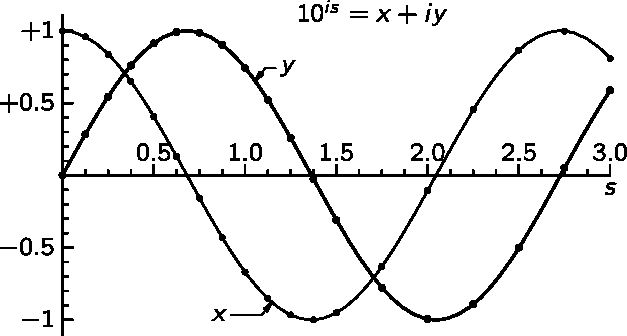
\includegraphics[width=1\linewidth]{fyz_fig0413.pdf}
      \caption{ (\cite[s.~306]{Feynman01})}
      \label{fyz:fig0413}
    \end{figure}

    Tuto kapitolu shrneme nejpozoruhodnějším vztahem matematiky
    \begin{equation}\label{fyz:eq696}
      e^{\imath θ}=\cosθ+\imath\sinθ.
    \end{equation}
    To je náš slibovaný skvost.

    Geometrii můžeme spojit s algebrou tak, že znázorníme komplexní čísla v rovině. Vodorovná poloha
    bodu je \(x\), svislá poloha je \(y\) (obr. \ref{fyz:fig0414}). Tak můžeme zobrazit každé
    komplexní číslo \(x + \imath y\). Nazveme-li radiální vzdálenost bodu \(r\) a úhel
    \(\varTheta\), platí algebraický zákon, že \(x + \imath y\) lze napsat jako re
    \(re^{\imath\varTheta}\), přičemž geometrické vztahy mezi \(x\), \(y\), \(r\) a \(\varTheta\)
    jsou znázorněny na obrázku. Tak vypadá sjednocení algebry a geometrie.

    Je i perioda stejná? Vypočítejme, na jakou mocninu je třeba umocnit \(e\), abychom dostali
    \(i\)? Jaký je logaritmus \(i\) při základu \(e\)? Pro základ \num{10} jsme to již počítali.
    Bylo by to \num{0.68226i}. Když přejdeme k základu \(e\), musíme to vynásobit \num{2.3025}, což
    je \num{1.5709}. Tuto hodnotu budeme nazývat „algebraickým \(\pi/2\)“. Vidíme však, že od
    správné hodnoty \(\pi/2\) se liší jen na posledním desetinném místě, což je způsobeno chybami v
    našich výpočtech! Nejdříve jsme tedy sestrojili čistě algebraickou cestou dvě nové funkce, sinus
    a kosinus, jež patří do algebry a jen do algebry. Nakonec jsme v nich však objevili právě ty
    funkce, s nimiž pracujeme v geometrii, takže mezi algebrou a geometrií zcela určitě existuje
    spojení.

    \begin{figure}[ht!] %\ref{fyz:fig0414}
      \centering
      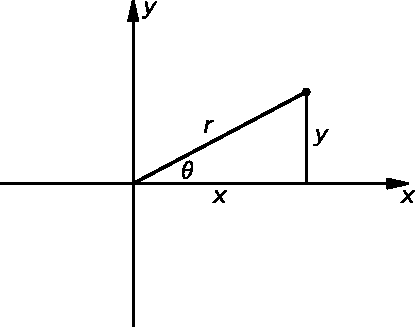
\includegraphics[width=0.9\linewidth]{fyz_fig0414.pdf}
      \caption{Grafické znázornění rovnice \(x + y = re^\imath\) (\cite[s.~306]{Feynman01})}
      \label{fyz:fig0414}
    \end{figure}

    Na začátku této kapitoly, když jsme byli vyzbrojeni jen Základními poznatky o přirozených
    číslech a tím, jak s nimi počítat, neuvědomovali jsme si sílu metody abstrakce a zobecnění.
    Použitím soustavy algebraických „zákonů“ nebo vlastností čísel (\ref{fyz:eq647}) a použitím
    definic inverzních operací (\ref{fyz:eq648}) jsme si sami dokázali vytvořit nejen nové druhy
    čísel, ale rovněž praktické věci, jako jsou tabulky logaritmů, mocnin a trigonometrických funkcí
    (což jsou vlastně imaginární mocniny reálných čísel), a to vše z deseti postupných druhých
    odmocnin desítky.

  \section{Komplexní čísla v Matlabu}\label{fyz:IchapXXIIsecVII}
    Jedna ze zajímavých vlastností Matlabu je možnost práce s komplexními čísly bez další potřebných
    knihoven. Komplexní čísla můžeme zadávat ve složkovém i exponenciálním tvaru. Imaginární
    jednotku zapíšeme jako \(\imath = \jmath = \sqrt{-1}\). Následující výpis obsahuje několik
    příkladů zadání komplexních čísel (\cite[s.~30]{Karban2006}).
    \begin{mdframed}[style=mdmsdos]
      \begin{lstlisting}[style=luaMatlabText,gobble=8]
        % slozkovy tvar - i
        >> c1 = 1-2i 
           c1 = 1.0000 - 2.0000i
        % slozkovy tvar - j
        >> c2 = 2-3j   
           c2 = 2.0000 - 3.0000i
        % exponenciální tvar
        >> c3 = 10*exp(pi/2*i)      
           c3 = 0.0000 + 10.0000i
      \end{lstlisting}
    \end{mdframed} 

    Pro vyjádření imaginární části komplexních čísel lze kromě \(\imath\) použít také \(\jmath\).
    Při počítání s komplexními čísly se také hodí následující funkce:
    \begin{description}
      \item[\texttt{real(c)}]    reálná část.
      \item[\texttt{imag(c)}]    imaginární část
      \item[\texttt{conj(c)}]    komplexní doplněk
      \item[\texttt{abs(c)}]     absolutní hodnota
      \item[\texttt{angle(c)}]   úhel \(\Theta\) v radiánech (obr. \ref{fyz:fig0414}) 
    \end{description}  

    Příkaz \texttt{compass} zobrazí vektory jako šipky směřující od středu souřadnice systému v
    Gaussově rovině:
    \begin{mdframed}[style=mdmsdos]
      \begin{lstlisting}[style=luaMatlabText,gobble=8]
        >> x = [1+0i, -1+0.5i, -0.3-0.4i]
           x = 1.0000 + 0.0000i  -1.0000 + 0.5000i  -0.3000 - 0.4000i
        >> compass(x)
      \end{lstlisting}
    \end{mdframed} 

    \luagraphic[1]{fyz_fig0932.pdf}{Kompasový graf vektorů jako šipek z počátku souřadnic 
      (\cite[s.~91]{Karban2006}}{fyz:fig0932}

  \section{Příklady a cvičení}\label{fyz:IchapXXIIsecVIII}
%---------------------------------------------------------------------------------------------------
}{ % DEBUG was off
  \LuaPartBckgrnd{fyz_title02.jpg}
  \LuaPartTitle{FYZ I}{Fyzika I}{FYZI}
  \parttoc
%==== Kapitola: Hlavní etapy vývoje fyziky =========================================================
% !TeX program = lualatex
% !TeX root = luaking.tex
% !TeX encoding = UTF-8
% !TeX spellcheck = cs_CZ
%---------------------------------------------------------------------------------------------------
% file fey1ch01_02_03.tex
%---------------------------------------------------------------------------------------------------
%===================== Kapitola: Základy fyziky ====================================================
\setchaptertoc
\chapter{Základy fyziky}\label{fyz:IchapI}
  \epigraph{\emph{Fyzika je jako sex, může přinést praktické výsledky, ale to není důvod, proč to 
    děláme.}}{Richard P. Feynmann}

  \begin{figure}[ht!]  % \ref{fyz:fig067}
    \centering
    \luafigure[0.6]{fyz_fig067.jpg}
    \caption{\wikiFeynman \textasteriskcentered 11. května 1918 - \textdagger 15. února 1988, 
             americký fyzik, který patřil k největším fyzikům 20. století}
    \label{fyz:fig067}
  \end{figure} 

  Možná nás napadne, zda není možné při studiu fyziky začít tak, že si nejdříve vypíšeme základní
  zákony a potom se budeme zabývat tím, co z nich vyplývá v nejrůznějších situacích. Tak se
  postupuje v euklidovské geometrii, kde se postulují axiomy, ze kterých se odvodí všechny možné
  závěry. Takovýmto způsobem však nemůžeme postupovat ze dvou důvodů. Především, zatím neznáme
  všechny základní zákony - oblast toho, co bychom ještě měli poznat, se nám stále zvětšuje. Dále,
  přesná formulace fyzikálních zákonů zahrnuje mnoho neobvyklých myšlenek, jejichž vyjádření si
  vyžaduje vyšší matematiku. Proto je nutná značná předběžná příprava jen k tomu, abychom rozuměli,
  co znamenají slova. Není tedy možné postupovat tímto způsobem. \emph{Učit se můžeme pouze
  postupně, kousek po kousku}.

  \section{Stěžejní myšlenky fyziky}\label{fyz:IchapIsecII}
    V této kapitole jsou zachyceny \emph{základní myšlenky}, s nimiž se ve fyzice setkáváme - 
    bude pojednáváno o tom, jaká je v současnosti představa o povaze věcí. Nebude však hovořeno o 
    tom, jak se poznala správnost těchto představ - o těchto detailech bude pojednáváno později, až 
    přijde ten pravý čas.

    Věci, o něž se ve fyzice zajímáme, se ukazují množstvím projevů a atributů. Stojíme-li 
    například na břehu a hledíme na moře, vidíme vodu, na vodě pěnu, nad mořem oblaka, slunce, 
    modrou oblohu a vůbec světlo, slyšíme zvuk, nárazy vln, svištění větru, cítíme vzduch. Na břehu 
    je písek a skály, a každá má jinou tvrdost a pevnost, barvu a složení. Jsou tam zvířata a vodní 
    tráva, je tam hlad i nemoc a na břehu je pozorovatel se svými myšlenkami a snad i štěstím. 
    Každé jiné místo v přírodě se vyznačuje podobnou pestrostí věcí a vlivů, podobnou složitostí. 
    Naše zvědavost nás nutí klást otázky, hledat souvislosti a chápat mnohotvárnost věcí jako 
    následek snad relativně malého počtu nejjednodušších věcí a sil působících nekonečně rozmanitě.
    
    Zadívejme se na obr. \ref{fyz:fig652} a položme si pár zdánlivě jednoduchých otázek: Je písek
    jiný než skály? Není snad písek nic jiného, než velký počet velmi malých kamínků? Je Měsíc velká
    skála? Kdybychom porozuměli tomu, co jsou skály, znamená to, že bychom pochopili i podstatu
    písku a Měsíce? Co je to vítr? Jsou to nárazy vzduchu podobné nárazům vody na břeh? Jaké
    společné rysy mají rozličné druhy pohybu? Co mají společného různé druhy zvuku? Kolik různých
    barev existuje? A tak dále. Takovým způsobem se snažíme postupně analyzovat všechny věci. Dáváme
    do souvislostí věci, které na první pohled vzájemně nesouvisí. Děláme to s nadějí, že se nám
    podaří redukovat počet rozličných věcí a tak je lépe poznat.

    \luagraphic[1]{fyz_fig652.jpg}{Je písek jiný než skály? Není snad písek nic jiného, než velký
      počet velmi malých kamínků? Jak se pohybuje mořská vlna? Proč loď plave? Fyzika nám umožňuje
      chápat materiální svět, v němž žijeme, a porozumět zákonům, jimiž se řídí.}{fyz:fig652}
    
    Před několika sty lety vznikla metoda hledání částečných odpovědí na uvedené otázky. 
    \emph{Pozorování, usuzování a experiment} vytvářejí to, co nazýváme \textbf{vědeckou metodou}. 
    Budeme se muset omezit jen na holý popis našich představ o tom, co se nazývá \emph{základní 
    fyzikou} nebo základními myšlenkami, které vznikly aplikováním vědecké metody.
    
    Co to znamená něco „pochopit“? Můžeme si představit, že to složité nahromadění pohybujících se 
    věcí, které vytvářejí „svět“, je šachová hra bohů a my vystupujeme jako diváci, kteří neznají 
    pravidla hry, ale je jim dovoleno hru \emph{pozorovat}. Samozřejmě, pozorujeme-li dostatečně 
    dlouho, můžeme nakonec pochytit několik pravidel. \emph{Pravidla hry} představují to, co 
    chápeme jako \emph{základní fyziku}. I  kdybychom znali všechna pravidla, nemuseli bychom ještě 
    rozumět každému kroku hry, protože je příliš složitá a možnosti našeho rozumu omezené. 
    Ten, kdo hraje šachy, jistě ví, že je jednoduché naučit se všechna pravidla, ale i tak je velmi 
    těžké zvolit ten správný tah nebo pochopit záměry protihráče. Stejné je to i s přírodou, jen 
    mnohem těžší. Máme však možnost najít alespoň všechna pravidla. Zatím je všechna neznáme. 
    (Každou chvíli se objevuje něco takového jako rošáda, kterou ještě neznáme.) Nejen, že neznáme 
    všechna pravidla, ale pomocí těch, která známe, umíme jen velmi málo vysvětlit. Je tomu tak 
    proto, že téměř všechny situace jsou ohromně složité a známá pravidla nám neumožní sledovat 
    všechny obraty hry, nemluvě o předvídání dalších kroků. Musíme se proto omezit na základnější 
    otázku pravidel hry. Naučíme-li se pravidla, budeme to považovat za „pochopení“ světa.
    
    Jak můžeme rozhodnout, zda pravidla, která vlastně jen „odhadujeme“, jsou skutečně správná, 
    když nemůžeme dokonale analyzovat hru? Existují zhruba tři způsoby. Především nám příroda může 
    poskytnout (nebo my si od přírody vynutíme) jednoduché situace skládající se z malého počtu 
    částí, umožňující přesnou předpověď budoucího dění, a tím i zkoušku pravidel. (V rohu 
    šachovnice zůstalo jen málo figurek, jejichž tahy již umíme přesně určit)

    \begin{tcnote}
      \textbf{Vědecká metoda} je posloupnost nebo sada procesů, používaných při vědeckém výzkumu.
      Cílem je získat znalosti a vědomosti pomocí pozorování a dedukce na základě dosud známých
      poznatků. Přijímání nových vědeckých poznatků je založeno na konkrétních důkazech. Vědecká
      metoda je založena na předpokladu, že kritériem pravdivosti vědecké hypotézy je souhlas
      předpovědí s výsledky výzkumu. Tento přístup udržuje vědecké \emph{hypotézy} v neustálém
      kontaktu s realitou a umožňuje jejich \emph{falzifikaci}, neboť hypotéza, jejíž důsledky jsou
      v rozporu s výzkumnými zjištěními, bude falzifikována. Mnohokrát ověřená hypotéza, kterou se
      zatím nepovedlo vyvrátit, se stává vědeckou teorií. Důsledkem je omezení vědy na otázky a
      hypotézy, jež jsou alespoň v principu rozhodnutelné pozorováním. Větší vědecký tým je však
      spíše konzervativní, což brzdí výzkum a vývoj.

      \textbf{Falzifikovatelnost} (vyvratitelnost nebo zpochybnitelnost) je ve filosofii vědy
      vlastnost takového vědeckého tvrzení, hypotézy nebo teorie, kterou je principiálně možné
      vyvrátit, například experimentem. Jinak řečeno, tvrzení nebo teorie je falzifikovatelná tehdy,
      pokud víme, jak by se dala vyvrátit čili negovat. Teorie, kterou experimenty potvrzují, sice
      platí, ale jen dokud ji nějaký experiment nevyvrátí. Problémem falzifikovatelnosti se
      především zabýval rakouský filozof kritického racionalismu Karl R. Popper, který zdůraznil, že
      žádný počet pokusných potvrzení nemůže vědeckou teorii definitivně dokázat. Na rozdíl od
      verifikace, která je vždy jen částečná, pouze falzifikace může být definitivní.

      {\centering
      \captionsetup{type=figure}
      \luafigure[0.7]{fyz_fig924.jpg}
      \captionof{figure}{\wikiPopper \textasteriskcentered	28. července 1902, Vídeň \textdagger 17.
        září 1994 (ve věku 92 let). Byl významným představitelem moderního liberalismu, teorie vědy
        a filosofie.Kredit: Wikipedia}
      \label{fyz:fig924}
      \par}

      Ve skutečnosti se jedná o podmínku testovatelnosti a vyvratitelnosti hypotéz a teorií.
      Princip, který takto formuloval, se podle něj nazývá \textbf{Popperova břitva} – „Vědecké
      teorie jsou ověřitelné. Ověřitelné teorie je možné na základě ověřovacího postupu zamítnout (a
      nahradit teoriemi jinými).“

      \tcblower
      Pravdivost vědecké teorie podle něj nelze dokazovat, ale jen empiricky testovat. Základem
      vědeckého poznání tedy není verifikace (potvrzení), ale falsifikace. Pouze ta teorie, kterou
      je možné podrobit falsifikaci, tedy vystavit ji možnosti vyvrácení, je vědecká, tím větší
      hodnotu má pro vědu. Netřeba hromadit důkazy, které teorii potvrzují; spíše hlídat to, co by
      ji mohlo vyvrátit. Konečnou, definitivní jistotu naší přesné znalosti pravdy nemůžeme mít
      nikdy, k pravdě se můžeme pouze přibližovat neustálým vylučováním falsifikovaných teorií,
      hovoříme o evoluci vědy. K evoluci, vývoji vědy dochází právě díky falzifikaci: tím, že něco
      popřeme, získáváme nový prostor pro otevření dalších, nových otázek.

      Důsledkem jeho pojetí vědeckého poznání je obrana otevřeného myšlení a otevřené společnosti.
      Síla vědy netkví tolik v tom, že se její tvrzení dají dokázat, nýbrž v tom, že musí být
      formulována tak, aby se dala vyvrátit. Právě tak síla demokracie nespočívá v tom, že by
      vybírala ty nejlepší k vládě, nýbrž že každou vládu lze běžnými prostředky (volbami) odvolat
    \end{tcnote}

    Druhý způsob zkoušky pravidel spočívá v jejich použití k odvození obecnějších pravidel. 
    Například, střelec se na šachovnici pohybuje úhlopříčně. Odtud je možné usuzovat na skutečnost, 
    že určitý střelec bude vždy na bílém poli. Odhlédneme-li od podrobností, můžeme prověřovat naše 
    pravidlo o pohybu uvedeného střelce tak, že sledujeme, jestli se vždy nachází na bílém poli. Po 
    dlouhém čase se samozřejmě může stát, že se náhle objeví na černém poli (v průběhu hry byl 
    vzat, ale jeden pěšec došel na konec šachovnice a proměnil se na střelce na černém poli). Tak 
    to bývá i ve fyzice. Dlouho používáme pravidlo, které ve všech směrech dobře vyhovuje, ačkoliv 
    neznáme detaily, a potom najednou objevíme \emph{nové pravidlo}. Z hlediska základů fyziky 
    probíhají nejzajímavější jevy na nových místech, na místech, kde pravidla neplatí a ne tam, kde 
    pravidla \emph{platí}. To je způsob, jakým objevujeme nová pravidla.

    Třetí ze způsobů, kterými se můžeme přesvědčit o správnosti našich myšlenek, je poměrně hrubý, 
    ale snad nejúčinnější. Je to způsob přibližného odhadu. Ačkoliv nejsme schopni říci, proč 
    Aljechin \emph{táhl právě tou figurkou}, můžeme v \emph{hrubých rysech} chápat, že seskupuje 
    figurky okolo krále, aby ho chránil, protože za daných okolností je to nejrozumnější. Podobně 
    je to i s naším chápáním přírody. Často ji více či méně chápeme, aniž bychom byli schopni znát 
    význam tahu \emph{každé jednotlivé figurky}.
    
    Zpočátku se přírodní jevy hrubě rozdělovaly do tříd jako teplo, elektřina, mechanika, 
    magnetizmus, vlastnosti látek, chemické děje, světlo nebo optika, rentgenové paprsky, jaderná 
    fyzika, gravitace, mezonové jevy atd. Cílem je však pochopení \emph{celé přírody} jako různých 
    aspektů \emph{jednoho souboru} jevů. Úkolem základní teoretické fyziky dneška je \emph{nalezení 
    zákonů stojících za experimentem a sjednocení uvedených tříd}. Historicky se nám vždy podařilo 
    sloučit je, ale postupem času se objevovaly nové věci. Když jsme si již vytvořili ucelenou 
    představu, objevily se najednou rentgenové paprsky. Když se i tento jev dostal do jednotného 
    schématu, objevily se mezony. Proto v každém stádiu hry vypadá situace dost chaoticky. Mnohé se 
    objasnilo z jednotného hlediska, ale ještě stále je mnoho volných konců nitek, o nichž nevíme, 
    kam patří. Takový je dnes stav věcí a my se ho pokusíme popsat.
    
    Všimněme si v historii několika příkladů uvedeného sjednocování. Uvažujme nejdříve \emph{teplo 
    a mechaniku}. Jsou-li atomy v pohybu, obsahuje systém tím více tepla, čím více pohybu v něm je, 
    takže \emph{teplo a všechny tepelné efekty je možné vyjádřit pomocí zákonů mechaniky}. Dalším 
    úžasným sjednocením bylo objevení souvislosti mezi \emph{elektřinou, magnetizmem} a světlem, o 
    nichž se zjistilo, že jsou různými aspekty stejné věci, kterou dnes nazýváme 
    \emph{elektromagnetické pole}. Dále chemické děje, rozmanité vlastnosti různých látek a chování 
    atomových částic byly sjednoceny do \emph{kvantové chemie}.
    
    Zůstává zde však otázka, zda bude možné vše sjednotit tak, abychom mohli prohlásit, že svět 
    představuje rozmanité aspekty jediné věci? To nikdo neví. Víme pouze, že na naší cestě vpřed se 
    nám daří spojovat fragmenty, přičemž vždy nalézáme cosi, co nezapadá do obecného obrazu, a 
    proto se opět pokoušíme doplnit skládačku. Nevíme, zda tato skládačka má konečný počet částí a 
    zda má tato hra vůbec hranice. Dozvíme se to až tehdy, když složíme výsledný obraz, jestli ho 
    vůbec kdy složíme. Chtěli bychom však ukázat, kam až tento proces sjednocování pokročil a jaká 
    je dnešní situace při objasňování základních jevů pomocí co nejmenšího počtu principů. 
    Jednodušeji řečeno: \textbf{z čeho jsou složeny věci a kolik je těch stavebních prvků?} 
    \cite[s.~27]{Feynman02}    


  \twocolumn[\section{Jak studovat fyziku podle Feynmana}\label{fyz:IchapIsecI}]
    Každý kousek nebo část celku, který představuje příroda, je vždy jen přiblížením k úplné pravdě;
    přesněji k úplné pravdě, pokud ji známe. Ve skutečnosti vše, co víme, je jen určitým druhem
    aproximace, protože víme, že ještě neznáme všechny zákony. Proto se věci musíme učit jen proto,
    abychom se je znovu odnaučili, nebo, což je pravděpodobnější, abychom si naše znalosti o nich
    opravovali.
    
    Princip vědy, téměř její definice, je následující: Prověrkou všech našich vědomostí je 
    experiment. Experiment je jediné kritérium vědecké „pravdy“. Jenže co je zdrojem našich 
    vědomostí? Odkud pocházejí zákony, které prověřujeme? Samotný experiment nám pomáhá odvozovat 
    zákony v tom smyslu, že nám poskytuje náznaky, pokyny. Navíc je však potřebná představivost, 
    aby z těchto náznaků mohla vzniknout velká zobecnění - abychom v nich odhadli nádherný, 
    jednoduchý, ale neobyčejný obraz a potom experimentem prověřili správnost našeho odhadu. Tento
    proces představivosti je tak těžký, že si fyzici rozdělili práci - teoretičtí fyzici 
    představivostí, dedukcí a odhadem odvozují nové zákony, ale neexperimentují; experimentální 
    fyzici dělají pokusy a přitom také uplatňují představivost, dedukci a odhad.
    
    Řekli jsme, že přírodní zákony jsou přibližné: že nejdříve nacházíme „nesprávné“ a až potom
    „správné“. Jak však může být experiment „nesprávný“? Především z velmi jednoduchého důvodu - náš
    přístroj není v pořádku a my jsme to nezpozorovali. Takové chyby se však zjišťují lehce.
    Odhlédneme-li od těchto drobností, jak může být výsledek experimentu nesprávný? Jen v důsledku
    nepřesnosti. Například, hmotnost předmětu se zdá být neměnná; rotující káča má stejnou hmotnost
    jako káča v klidu. Tak byl objeven „zákon“: hmotnost je konstantní, nezávislá na rychlosti. O
    tomto „zákonu“ se zjistilo, že je nesprávný. Ukázalo se, že hmotnost roste s rychlostí, ale k
    značnému růstu jsou potřebné rychlosti blízké rychlosti světla. Správný zákon zní: je-li
    rychlost tělesa menší než \SI{100}{\km\per\second}, je hmotnost konstantní s přesností na jednu
    milióntinu. V takové aproximativní podobě je tento zákon správný. Někdo by si mohl myslet, že
    prakticky není rozdíl mezi starým a novým zákonem. To je i není pravda. Pro běžné rychlosti je
    jistě možné zapomenout na to, o čem jsme mluvili a používat jednoduchý zákon konstantní
    hmotnosti jako dobré přiblížení. Při velkých rychlostech se však dopustíme chyby, a to tím
    větší, čím větší je rychlost

    \begin{figure}[ht!]  %\ref{fyz:fig891}
      \centering
      \luafigure[0.9]{fyz_fig891.jpg}
      \caption{Vodní kapka dopadající na hladinu. Kredit: Wikipedia}
      \label{fyz:fig891}
    \end{figure} 
    
    Ostatně, nejzajímavější je to, že z filozofického hlediska je tento aproximativní zákon zcela
    nesprávný. Náš celkový obraz o světě musíme změnit, i kdyby se hmotnost měnila jen nepatrně.
    Toto je svérázný znak filozofie nebo myšlenek stojících v pozadí zákonů. Někdy i velmi malý
    efekt vyžaduje hlubokou změnu našich názorů.
    
    Čemu tedy máme dát přednost? Máme podat správné, ale nezvyklé zákony s jejich cizím a obtížným
    pojetím jako je například teorie relativity, čtyřrozměrný prostoročas a podobně? Nebo máme
    nejdříve vysvětlit jednoduchý zákon „konstantní hmotnosti“, který je pouze přibližný, ale
    nevyžaduje náročné představy? První způsob je více vzrušující, nádhernější a zábavnější, ale s
    druhým se jednodušeji začíná a představuje první krok ke skutečnému porozumění správného zákona.
    Tento problém se vždy znovu objevuje při vyučování fyziky. V různých etapách ho musíme řešit
    různými způsoby, ale vždy je vhodné se zajímat, do jaké míry je přesné to, co teď víme, jak to
    souvisí s dalším a jak se to může změnit, budeme-li vědět víc.
    
    Nyní přejděme k náčrtu nebo k všeobecné mapě našeho chápání současné vědy (zejména fyziky, ale i
    jiných věd, které s ní souvisejí). Když se později soustředíme na konkrétní problém, budeme mít
    představu o jeho pozadí, o tom, proč je zajímavý a jak zapadá do celkové struktury. Jaký je tedy
    náš celkový obraz světa? \cite[s.~16]{Feynman01}
    
  \section{Látka se stává z atomů}
    Kdyby při nějaké katastrofě zanikly všechny vědecké poznatky a dalším generacím by měla zůstat
    jen jediná věta, které tvrzení by při nejmenším počtu slov obsahovalo nejbohatší informaci?
    Takovým kandidátem je \textbf{atomová hypotéza} - tj. že \emph{všechny věci se skládají z atomů
    malých částic, jež jsou v neustálém pohybu,  a vzájemně se přitahují, když jsou od sebe trochu
    vzdálené, ale odpuzují se, když jsou těsně u sebe.} V této jediné větě, jak uvidíme, je obsaženo
    nesmírné množství informací o světě. Je k tomu třeba jen trochu představivosti a uvažování.

    \begin{figure}[ht!]  %\ref{fyz:fig007}
      \centering
      \luafigure[0.6]{fyz_fig007.pdf}
      \caption{Vodní kapka z obrázku \ref{fyz:fig891} zvětšená miliardkrát \cite[s.~17]{Feynman01}}
      \label{fyz:fig007}
    \end{figure} 

    Abychom ilustrovali sílu myšlenky o atomu, představme si podobnou kapku vody jako na obrázku
    \ref{fyz:fig891} o rozměru \SI{0.5}{\cm}. Podí\-váme-li se na ni zblízka, neuvidíme nic jiného,
    než vodu - klidnou, souvislou vodu. I když kapku zvětšíme tím nejlepším optickým mikroskopem,
    přibližně dvoutisíckrát, a kapka bude měřit deset metrů, tedy stejně jako velká místnost, i
    tehdy budeme stále vidět relativně klidnou vodu. Jen tu a tam v ní budou plavat jakési malé
    fotbalové míče. Tyto velmi zajímavé objekty na obrázku \ref{fyz:fig890} jsou trepky. Tady se
    můžeme zastavit a zajímat se o trepky, o jejich třepotající se řasičky, o jejich kroutící se
    těla a nepokračovat ve zvětšování. Nebo můžeme zvětšit trepky tak, abychom viděli i do nich). 

    \begin{figure}[ht!]  %\ref{fyz:fig890}
      % http://www.photomacrography.net/forum/viewtopic.php?t=18166
      \centering
      \luafigure[1]{fyz_fig890a.jpg}
      \caption{ Trepka velká \emph{(Paramecium caudatum)} je nálevník běžně se vyskytující v 
                organicky znečištěných vodách po celém světě. Kredit: Wikipedia}
      \label{fyz:fig890}
    \end{figure} 

    Trepky jsou však předmětem biologie. Proto si jich teď nebudeme všímat, ale zahledíme se ještě
    pozorněji na vodu při dalším dvoutisícinásobném zvětšení. Teď měří kapka vody dvacet kilometrů a
    při pozorném sledování je vidět jakési hemžení - cosi, co už nevypadá klidně, ale připomíná dav
    na fotbalové tribuně při pohledu z velké vzdálenosti. Abychom zjistili, co je to za hemžení,
    zvětšíme kapku ještě 250krát a potom uvidíme něco podobného jako na obr. \ref{fyz:fig007}. Tento
    obrázek představuje vodu při zvětšení miliardkrát, je však v několika směrech idealizovaný.
    Především částice jsou zakreslené zjednodušeně - s ostrými okraji, což neodpovídá skutečnosti.
    Dále kvůli jednoduchosti jsou částice zakreslené v dvojrozměrném uspořádání, ačkoli se ve
    skutečnosti pohybují ve všech třech směrech. Všimněme si, že jsou tam dva druhy částic
    znázorněných kroužky, které představují atomy kyslíku (černé) a vodíku (bílé) a že na každý atom
    kyslíku se vážou dva atomy vodíku. Každá skupinka skládající se z atomu kyslíku a dvou atomů
    vodíku se nazývá \textbf{molekulou}. Obrázek je zjednodušený i v tom, že skutečné částice v
    přírodě se ustavičně kolébají a poskakují, obracejí se a točí jedna okolo druhé. Je třeba si to
    představit spíše jako \emph{dynamický a né jako statický obrázek}. Další věcí, kterou není možné
    vystihnout na obrázku, je skutečnost, že částice „drží pohromadě“ - přitahují se, jedna za sebou
    táhne druhou atd. Je možné říci, že jsou jakoby „slepené dohromady“. Na druhé straně se částice
    netlačí jedna přes druhou. Kdybychom se pokusili přitlačit dvě z nich příliš těsně k sobě,
    odpudily by se.

    Atomy mají poloměr \SI{1e-10}{\m} až \SI{2e-10}{\m}. Jejich velikost si můžeme pamatovat i
    jinak: zvětšíme-li jablko na velikost Země, budou atomy v jablku tak velké, jak bylo původně
    jablko.

    Představme si teď tuto velkou kapku vody s jejími hemžícími se částicemi, jež přilnuly k sobě a
    honí jedna druhou. Voda udržuje svůj objem; nerozpadne se na části díky vzájemné přitažlivosti
    molekul. Je-li tato kapka na šikmé ploše, kde se může hýbat z místa na místo, voda poteče.
    Nestane se však, že by jednoduše zmizela. Věci se nerozpadají na části právě díky přitažlivosti
    molekul. \emph{Hemživý pohyb částic je to, co chápeme jako teplo}: zvýšíme-li teplotu, zvětšíme
    pohyb. Zahříváme-li vodu, pohyb roste a roste i vzdálenost mezi částicemi, až nastane okamžik,
    kdy přitažlivost mezi molekulami je už nestačí udržet pohromadě. Částice přestanou být vzájemně
    svázané a rozlétají se od sebe. Zvyšováním teploty tak získáváme \emph{vodní páru}.  
    
    \begin{figure}[ht!]
      \centering
      \luafigure[0.6]{fyz_fig008.pdf}
      \caption{Pára \cite[s.~18]{Feynman01}}
      \label{fyz:fig008}
    \end{figure}

    Na obr. \ref{fyz:fig008} vidíme páru. V jednom směru tento obrázek páry selhává: při našem
    zvětšení za normálního atmosférického tlaku připadá jen velmi málo molekul na celý pokoj, takže
    na tak malém obrázku určitě nebudou tři molekuly. Většina plošek této velikosti nebude obsahovat
    žádnou molekulu - na našem obrázku jsou náhodou dvě a část z třetí molekuly (abychom tam neměli
    prázdné místo). V případě páry vidíme podobu molekul jasněji než v případě vody. Pro
    jednoduchost jsou molekuly zakresleny tak, že atomy vodíku svírají úhel \SI{120}{\degree}. Ve
    skutečnosti má tento úhel hodnotu \ang[arc-separator = \,]{105;3;} a vzdálenost mezi středem
    vodíku a středem kyslíku je \SI{9.57e-11}{\m}. Tuto molekulu tedy velmi dobře známe.

    Všimněme si jedné vlastnosti vodní páry nebo jiných plynů. Molekuly budou tím, že se vzdálily
    jedna od druhé, narážet na stěny. Představme si místnost s určitým počtem (tak kolem sta)
    neustále poskakujících tenisových míčků. Když míčky narážejí na stěnu, odtlačují ji a stěnu
    proto musíme upevnit. Plyn působí přerušovanou silou, kterou naše nedokonalé smysly (jejich
    citlivost nevzrostla miliardkrát) vnímají jako \emph{stálý tlak}. Abychom plyn udrželi, musíme
    na něj působit tlakem z opačné strany. Obr. \ref{fyz:fig009} znázorňuje běžnou nádobu na
    udržování plynu, kterou najdeme v každé učebnici: \textbf{válec s pístem}. Teď nám nezáleží na
    tom, jaký je ve skutečností tvar molekul vody, a proto je kvůli jednoduchostí znázorníme jako
    tenisové míčky nebo body. Jsou v neustálém pohybu a pohybují se na všechny strany. Na spodek
    \emph{pístu} jich neustále naráží tolik, že na něj musíme působit určitou silou dolů, aby ho
    molekuly nevytlačily z válce. Tuto \emph{sílu} nazýváme \textbf{tlakem} (přesněji, \emph{tlak
    násobený plochou dává sílu}). Je jasné, že síla je úměrná ploše pístu, protože zvětšíme-li
    plochu a přitom nezměníme počet molekul v kubickém centimetru, pak vzroste počet srážek s pístem
    tolikrát, kolikrát se zvětšila jeho plocha.

    \begin{figure}[ht!]
      \centering
      \luafigure[0.4]{fyz_fig009.pdf}
      \caption{Píst \cite[s.~18]{Feynman01}}
      \label{fyz:fig009}
    \end{figure}

    Nyní \emph{zdvojnásobme} v této nádobě počet molekul, takže se zdvojnásobí jejich hustota, ale
    ponechme jim stejnou rychlost, tj. \emph{stejnou teplotu}. Pak můžeme dost přesně říci, že se
    zdvojnásobil počet srážek a jelikož je každá právě tak \uv{energická} jako dříve, tlak je úměrný
    hustotě. Uvážíme-li skutečnou povahu meziatomových sil, můžeme očekávat mírný pokles tlaku jako
    projev zvýšené přitažlivosti mezi atomy a mírný vzrůst související s objemem, který zaujímají.
    Přesto však, pokud je hustota dostatečně nízká, tj. atomů není příliš mnoho, můžeme s
    dostatečnou přesností říci, že \emph{tlak je úměrný hustotě}.
    
    Snadno pochopíme i něco jiného. \emph{Zvyšujeme-li teplotu} bez změny hustoty plynu, tj. když
    zvětšujeme rychlost atomů, co se stane s tlakem? Atomy narážejí do pístu \emph{silněji}, neboť
    se pohybují rychleji a navíc, narážejí častěji. Proto tlak vzrůstá. Vidíme, jak jednoduché jsou
    myšlenky atomové teorie.
    
    Podívejme se na jinou situaci. Předpokládejme, že se píst \emph{pohybuje dovnitř}, takže atomy
    jsou pomalu stlačovány do menšího prostoru. Co se stane, narazí-li atom do pohybujícího se
    pístu? Je jasné, že při takové srážce \emph{získá rychlost}. Můžeme si to vyzkoušet na
    ping-pongovém míčku: po úderu pálkou míček odletí od pálky rychleji, než k ní přiletěl. Ve
    zvláštním případě, není-li atom v pohybu a píst na něj narazí, atom se začne určitě pohybovat.
    Atomy jsou při návratu od pístu \uv{teplejší}, než byly před nárazem na píst. Proto všechny
    atomy, které jsou v nádobě, získají na rychlosti. To znamená, že při pomalém \emph{stlačení
    plynu jeho teplota vzrůstá}. Když plyn pomalu \emph{stlačujeme}, jeho teplota \emph{vzrůstá} a
    když plyn pomalu \emph{rozpínáme}, jeho teplota \emph{klesá}.
    
    \begin{figure}[ht!]  % \ref{fyz:fig010}
      \centering
      \luafigure[0.6]{fyz_fig010.pdf}
      \caption{Led \cite[s.~19]{Feynman01}}
      \label{fyz:fig010}
    \end{figure}

    Vraťme se k naší kapce vody a podívejme se na ni z jiného pohledu. Snižme teplotu naší kapky.
    Předpokládejme, že hemžení molekul vody postupně slábne. Víme, že mezi atomy působí přitažlivé
    síly, které způsobí, že molekuly už nebudou moci tak snadno pohybovat. Obr. \ref{fyz:fig010}
    znázorňuje, co se stane při velmi nízkých teplotách: molekuly jsou vázány v nové struktuře,
    vytváří se \textbf{led}. Takové schematické znázornění ledu není správné, neboť je dvojrozměrné.
    Situaci však vystihuje kvalitativně. Je pozoruhodné, že každý atom má v této látce určité místo.
    Rozmístíme-li atomy na jednom konci kapky podle určitého pravidla, pak v důsledku pevné
    struktury meziatomových vazeb vznikne určité uspořádání atomů i na druhém konci kapky, vzdáleném
    (v našem měřítku) několik kilometrů. Proto, držíme-li ledový rampouch za jeden konec, jeho druhý
    konec bude při lámání klást odpor, chová se jinak než voda, ve které je pravidelná struktura
    rozrušena intenzívním pohybem atomů v rozličných směrech. Rozdíl mezi pevnými látkami a
    kapalinami spočívá v tom, že atomy pevné látky jsou \emph{uspořádány} zvláštním způsobem. Toto
    uspořádání se nazývá \textbf{krystalická struktura}. I tehdy, kdy jde o velmi vzdálené atomy,
    nepozorujeme nic náhodného v jejich polohách. Poloha atomu na jednom konci krystalu je určena
    polohou atomu na druhém konci, i když se mezi nimi nacházejí miliony jiných atomů. Obr.
    \ref{fyz:fig010} znázorňuje vymyšlené uspořádání ledu a ačkoli správně vystihuje mnohé
    vlastnosti ledu, neodpovídá skutečnému uspořádání. Jedním ze správných rysů je existence části
    \emph{hexagonální symetrie}. Můžeme se o tom přesvědčit: otočíme-li obrázek o \SI{120}{\degree},
    dostaneme stejné seskupení. Taková symetrie ledu je příčinou šestihranného tvaru sněhových
    vloček. Další informací, kterou je možné vytušit z obrázku \ref{fyz:fig010}, je \emph{zmenšování
    objemu ledu při tání}. Znázorněná struktura ledu, stejně tak jako skutečná, obsahuje \emph{mnoho
    dutin}. Když se struktura rozpadne, tyto dutiny mohou být \emph{zaplněny} molekulami.
    \emph{Většina jednoduchých látek, s výjimkou vody a liteřiny\footnote{Liteřina či písmovina je
    slitina používaná v písmolijectví. Její přibližné složení je: \SIrange{50}{86}{\percent} olova,
    \SIrange{3}{20}{\percent} cínu a \SIrange{11}{30}{\percent} antimonu. Liteřinu vyvinul v 15.
    století zakladatel knihtisku Johannes Gutenberg pro odlévání tiskařských liter.}, zvětšují při
    tání svůj objem, neboť atomy jsou v pevných krystalech těsně seskupeny a při tání potřebují více
    prostoru na kmitání}. Otevřené struktury se však při tání zhroutí - podobně jako led.
    
    I když má led pevnou krystalickou strukturu, jeho teplota se může měnit - v ledu je zásoba 
    tepla. Chceme-li, můžeme toto množství tepla změnit. Jaké je teplo, které se nachází v ledu? 
    Atomy ledu \emph{nejsou} v klidu, poskakují a kmitají. Ačkoli v krystalu existuje určité 
    uspořádání - struktura - všechny atomy kmitají, „na místě“. Zvyšujeme-li teplotu, budou 
    kmitat se stále větší amplitudou, až opustí svá místa. Tento jev nazýváme \textbf{táním}. 
    Snižujeme-li teplotu, kmity slábnou a při teplotě \emph{absolutní nuly} jsou 
    \emph{nejslabší}, ne však nulové. Toto nejmenší množství pohybu, který přísluší atomům, 
    nestačí na roztání látky - až na jednu výjimku: \emph{hélium}. V héliu se při ochlazování 
    také zpomaluje pohyb atomů na nejmenší možnou míru, ale i při teplotě absolutní nuly brání 
    tento pohyb zmrznutí hélia. Hélium nezmrzne, pokud nevytvoříme tak veliký tlak, abychom atomy 
    stlačili k sobě. Při velkém tlaku můžeme dosáhnout toho, že hélium ztuhne.
  
  \subsection{Atomové procesy}
    Dosud jsme si všímali stavby pevných látek, kapalin a plynů z atomového hlediska. Jenže atomová
    hypotéza charakterizuje i procesy, a proto si všimněme některých procesů z atomového hlediska.
    Nejdříve budeme hovořit o procesech, které se odehrávají na povrchu vody. Co se vlastně děje na
    vodním povrchu? Úlohu si zkomplikujeme - bude tak blíže skutečnosti - předpokladem, že nad
    vodním povrchem se nachází vzduch. Obr. \ref{fyz:fig011} takovou situaci znázorňuje. Tak jako
    předtím vidíme molekuly vody, které tvoří kapalinu, ale vidíme i povrch vody. Nad povrchem
    vidíme různé molekuly. Jsou tam především \emph{molekuly vody} v podobě vodní páry, kterou je
    možné pozorovat vždy nad kapalnou vodou (pára a voda jsou v rovnováze, o které pohovoříme
    později). Dále tam nalezneme jiné molekuly, dvojice atomů kyslíku tvořící \emph{molekulu
    kyslíku} a dvojice atomů dusíku tvořící \emph{molekulu dusíku}. Vzduch se skládá téměř výhradně
    z dusíku, kyslíku, vodní páry a menšího množství oxidu uhličitého, argonu a jiných příměsí. Nad
    povrchem vody se nachází vzduch - plyn obsahující jisté množství vodní páry. Nyní si všimněme,
    co se odehrává na obrázku. Molekuly vody se neustále pohybují. Občas některá z molekul,
    nacházejících se v blízkosti povrchu, naráží na jinou molekulu trochu silněji než obvykle a
    vyskočí nad povrch. Na obrázku takovýto děj \emph{přímo} neuvidíme, neboť vše je na něm nehybné.
    Můžeme si však představit, že jedna molekula za druhou v důsledku srážek opouštějí vodu - voda
    mizí, \emph{vypařuje} se. Když nádobu \emph{přikryjeme}, objevíme po nějakém čase velké množství
    molekul vody mezi molekulami vzduchu. Čas od času některá z těchto molekul vody vletí zpět do
    vody a zůstává v ní. To, co jsme považovali za mrtvé a nezajímavé - přikrytý pohár vody, který
    snad dvacet let stál na jednom místě - v sobě skrývá stále probíhající zajímavý
    \textbf{dynamický proces}. Náš nedokonalý zrak nepozoruje žádnou změnu, ale při miliardovém
    zvětšení bychom viděli, jak se vše mění: jedny molekuly opouštějí povrch a druhé se vracejí.
    
    \begin{figure}[ht!]   % \ref{fyz:fig011}
      \centering
      \luafigure[0.7]{fyz_fig011.pdf}
      \caption{Voda vypařující se do vzduchu \cite[s.~21]{Feynman01}.}
      \label{fyz:fig011}
    \end{figure}

    Proč nepozorujeme tyto změny my? Protože do vody se vrací právě tolik molekul, kolik z ní
    odešlo. Navenek se „nic neděje“. Když odkryjeme nádobu, odfoukneme vlhký vzduch pryč a nahradíme
    ho suchým vzduchem, nezmění se počet z vody vylétajících molekul (neboť závisí pouze na pohybu
    ve vodě), ale velmi se změní počet molekul do vody se vracejících, protože nad vodou je mnohem
    méně molekul. Molekul, které opouštějí vodu, je víc než molekul, které se do ní vracejí; voda se
    vypařuje. Chceme-li tedy, aby se voda vypařovala, zapneme ventilátor!
    
    Zůstává ještě otázka: Které molekuly opouštějí vodu? Molekula opustí vodu, když náhodně získá
    malé množství dodatečné energie, kterou potřebuje na to, aby překonala přitažlivé působení svých
    sousedů. Protože ty molekuly, které opouštějí vodu, mají větší než průměrnou energii, budou se
    molekuly, které ve vodě zůstávají, v průměru pohybovat méně. Při vypařování se tedy kapalina
    postupně \emph{ochlazuje}. Je samozřejmé, že když molekula páry sestoupí ze vzduchu do vody,
    objeví se silné přitahování, když molekula dosahuje povrchu vody. Důsledkem toho je zrychlení
    přicházející molekuly a s tím spojený vznik tepla. \emph{Můžeme tedy říci, že s odchodem molekul
    odchází a s příchodem molekul přichází teplo.} Když jsou oba procesy vyrovnány, voda svou
    teplotu nemění. Foukáme-li na vodu, aby odpařování převládalo nad zkapalňováním, voda se
    ochlazuje. Proto, chcete-li ochladit polévku, foukejte na ni!
    
    \begin{figure}[ht!]    % \ref{fyz:fig012}
      \centering
      \luafigure[0.7]{fyz_fig012.pdf}
      \caption{Sůl rozpouštějící se ve vodě \cite[s.~21]{Feynman01}.}
      \label{fyz:fig012}
    \end{figure}

    Musíme si však uvědomit, že procesy, o kterých jsme hovořili, probíhají ve skutečnosti
    složitěji. Při unikání vody do vzduchu čas od času některá z molekul kyslíku nebo dusíku vnikne
    do vody a \uv{ztratí se} mezi jejími molekulami. Vzduch se tedy rozpouští ve vodě. Molekuly
    kyslíku a dusíku pronikají do vody, která pak obsahuje vzduch. Když z nádoby náhle odstraníme
    vzduch, budou molekuly vzduchu unikat z vody rychleji, než do ní vnikají, což způsobí
    vystupování bublinek. Tato skutečnost je velmi nepříjemná pro potápěče.
  
    Nyní si všimněme dalšího procesu. Obr. \ref{fyz:fig012} znázorňuje, jak se podle atomové
    představy rozpouští pevná látka ve vodě. Co se stane, vložíme-li krystal soli do vody? Sůl je
    pevná látka, krystal, organizované seskupení „atomů soli“. Na obr. \ref{fyz:fig013} je
    znázorněna trojrozměrná struktura kuchyňské soli, chloridu sodného. Máme-li být přesní, musíme
    říct, že krystal není tvořen atomy, ale ionty. Iont je atom, který má několik elektronů navíc,
    nebo několik elektronů ztratil. V krystalu soli nalézáme \emph{ionty chlóru} (atomy chlóru s
    přebytečným elektronem) a \emph{ionty sodíku} (atomy sodíku zbavené jednoho elektronu). Ionty
    jsou v krystalu vzájemně vázány elektrickou přitažlivostí, ale ve vodě se některé z nich pod
    vlivem přitažlivosti záporného kyslíku a kladného vodíku začnou uvolňovat. Na obrázku
    \ref{fyz:fig012} vidíme uvolňující se iont chlóru a jiné atomy plavající ve vodě ve formě iontů.
    Tento obrázek je pečlivě zakreslený. Všimněme si například, že vodíkové konce molekul vody
    obvykle obklopují iont chlóru a u iontu sodíku zpravidla nalézáme kyslíkový konec, neboť sodík
    je kladný a kyslíkový konec molekuly vody je záporný a tyto se elektricky přitahují. Můžeme
    podle tohoto obrázku říci, jestli se sůl \emph{rozpouští} ve vodě, nebo \emph{krystalizuje} z
    vody? Samozřejmě, že \emph{nemůžeme}, neboť zatím co jedny atomy opouštějí krystal, jiné se k
    němu připojují. Takovýto proces je - podobně jako vypařování - \emph{dynamický} všechno závisí
    na tom, je-li ve vodě více nebo méně soli, než je třeba k rovnováze. Rovnováhou rozumíme takovou
    situaci, kdy počet atomů opouštějících krystal je roven počtu atomů do krystalu se vracejících.
    Když sůl ve vodě téměř není, vstupuje do vody více atomů, než vystupuje a sůl se rozpouští. Když
    je, naopak, „atomů soli“ příliš mnoho, do krystalu se vrací více atomů, než ho opouští a sůl
    krystalizuje.

    \begin{figure}[hbt!]  % \ref{fyz:fig013}
      \centering
        \subcaptionbox{\label{fyz:fig013a}}{\luafigure[0.4]{fyz_fig013a.pdf}}   \\                                   
        \subcaptionbox{\label{fyz:fig013b}}{\luafigure[0.8]{fyz_fig013b.pdf}}
      \caption{Vzdálenost nejbližších sousedů \(d = \dfrac{a}{2}\) \cite[s.~22]{Feynman01}}
      \label{fyz:fig013}
    \end{figure}
    
    Zmínili jsme se o tom, že představa \emph{molekuly} látky je pouze přibližná a je opodstatněná
    jen pro určitou třídu látek. Je jasné, že v případě vody jsou její tři atomy skutečně svázané,
    ale v případě pevného chloridu sodného už to tak jasné není. V takovém případě jde o uspořádání
    sodíkových a chlorových iontů do krychlové mřížky a neexistuje přirozený způsob jejich
    uspořádání do „molekul soli“.
    
    Vraťme se ještě k naší diskuzi o \emph{rozpouštění a srážení}. Zvýšíme-li teplotu roztoku soli,
    vzroste počet atomů, které sůl opouštějí a vzroste i počet atomů, které se do soli vracejí.
    Ukazuje se, že obecně je velmi těžké předpovědět, jak se ten proces realizuje, proběhne-li
    rozpouštění rychleji nebo pomaleji. S rostoucí teplotou se většina látek rozpouští lépe, ale
    některé látky se rozpouštějí hůře.
    
  \subsection{Chemické reakce}
    Ve všech procesech, o nichž jsem dosud hovořili, neměnily atomy a ionty své partnery. Za
    určitých okolností však může dojít ke změně atomových kombinací, vytvoří se nové molekuly.
    Taková situace je znázorněna na obr. \ref{fyz:fig014}.
    
    \begin{figure}[hbt!]   % \ref{fyz:fig014}
      \centering
      \luafigure[0.7]{fyz_fig014.pdf}
      \caption{Uhlík hořící v kyslíku \cite[s.~23]{Feynman01}}
      \label{fyz:fig014}
    \end{figure}

    Proces, ve kterém dochází k přeskupení atomových partnerů, nazýváme \textbf{chemickou reakcí}.
    Ostatní dosud uvažované procesy nazýváme \textbf{fyzikálními procesy}. Mezi uvedenými dvěma
    druhy, procesů však neexistuje ostrá hranice. Příroda se nestará o naše názvosloví a pokračuje i
    nadále ve svém díle. Uvedený obrázek má znázornit hoření uhlíku v kyslíku. Kyslík se vyznačuje
    tím, že jeho dva atomy jsou velmi pevně svázány. (Proč nejsou svázány \emph{tři} nebo dokonce
    \emph{čtyři} atomy? Toto je jedna ze zvláštností atomových procesů. Atomy jsou velmi svérázné:
    upřednostňují určité partnery, určité směry apod. Úlohou fyziky je analyzovat, proč chtějí právě
    to, co chtějí. V každém případě dva atomy kyslíku, nasycené a šťastné, tvoří molekulu.)
    
    Předpokládejme, že atomy uhlíku vytvářejí pevný krystal - grafit nebo diamant (diamant může
    shořet ve vzduchu). Uvažujme situaci, kdy se molekula kyslíku dostane k uhlíku, Každý její atom
    zachytí atom uhlíku a odletí v novém seskupení - „uhlík-kyslík“. Toto seskupení představuje
    molekulu plynu nazývaného \emph{oxid uhelnatý}. Jeho chemické označení je \ce{CO}. Je to velmi
    jednoduché: písmena „CO“ jsou vlastně obrazem jeho molekuly. Jenže uhlík váže kyslík o mnoho
    silněji než kyslík váže kyslík nebo uhlík váže uhlík. Proto v tomto procesu může kyslík
    přicházet s malou energií, ale kyslík a uhlík se spojí velmi „energicky“a uvolněnou energii
    pohltí okolní atomy. Tak se vytváří velké množství pohybové, kinetické energie. Myslíme tím
    samozřejmě \textbf{hoření}; spojením uhlíku a kyslíku získáváme \emph{teplo}. Teplo se obvykle
    projevuje formou pohybu molekul horkého plynu, ale za určitých okolností ho může být tak mnoho,
    že způsobuje světlo. Tak vzniká \textbf{plamen}.
    
    \begin{figure}[hbt!]    % \ref{fyz:fig015}
      \centering
      \luafigure[0.7]{fyz_fig015.pdf}
      \caption{Vůně fialek \cite[s.~24]{Feynman01}}
      \label{fyz:fig015}
    \end{figure}

    Kromě toho, \emph{oxid uhelnatý} není zcela uspokojen. Je možné, aby k sobě připoutal další atom
    kyslíku a tak dostaneme mnohem složitější reakci, ve které se kyslík spojuje s uhlíkem a
    současně dochází ke srážce s molekulou oxidu uhelnatého. Kyslíkový atom se připojí k \ce{CO} a v
    konečném důsledku vytvoří molekulu složenou z jednoho uhlíku a dvou kyslíků. Tato molekula má
    označení \ce{CO2} a nazývá se \emph{oxid uhličitý}. Spalujeme-li uhlík ve velmi malém množství
    kyslíku a reakce probíhá velmi rychle (např. v motoru automobilu, kde je výbuch tak rychlý, že
    se nestačí vytvořit oxid uhličitý), vzniká velké množství oxidu uhelnatého. V mnoha takových
    přeskupeních atomů se uvolňuje velké množství energie, vznikají výbuchy, plamen apod., podle
    druhu reakce. Chemici studovali takové seskupení atomů a zjistili, že každá látka představuje
    určitý druh \emph{uspořádání atomů}.

    K objasnění této myšlenky si zvolme jiný příklad. Ocitneme-li se na louce rozkvetlé fialkami,
    víme, co je to za „vůni“. Je to určitý druh molekul nebo seskupení atomů, které se dostalo do
    našeho nosu. Jak se nám to stalo? To je dost jednoduché! Jestliže vůně je jistý druh molekul,
    tím nejrozmanitějším způsobem poletujících a srážejících se ve vzduchu, pak se může náhodou
    dostat i do nosu. Tyto molekuly se určitě nesnažily dostat právě do našeho nosu. Jsou jen
    bezmocnou částí strkajícího se zástupu molekul, jehož kousek se na svém bezcílném putování
    dostal do našeho nosu.      
    
    Chemici mohou i takové zvláštní molekuly, jako je vůně fialek, podrobit analýze a říci nám
    \emph{přesné uspořádání} jejich atomů v prostoru. Víme, že molekula oxidu uhličitého je
    \emph{přímá a symetrická}: \ce{O\bond{-}C\bond{-}O} (lze to snadno zjistit i fyzikálními
    metodami). I pro mnohem složitější seskupení atomů, jako jsou ty, se kterými pracuje chemie,
    můžeme zdlouhavým, pozoruhodným procesem, připomínajícím práci detektiva, zjistit tvar
    seskupení. Obr. \ref{fyz:fig015} znázorňuje vzduch v blízkosti fialky: ve vzduchu opět nalézáme
    dusík, kyslík a vodní páru. (Odkud se vzala vodní pára? Fialka je vlhká, protože všechny
    rostliny odpařují vodu.) Vidíme však i \uv{monstrum} složené z uhlíkových, vodíkových a
    kyslíkových atomů, které vytvořily zcela určité, zvláštní seskupení. Je to mnohem složitější
    seskupení než v případě oxidu uhličitého. Naneštěstí do obrázku nemůžeme zakreslit všechno, co o
    něm po chemické stránce víme, neboť seskupení všech atomů je trojrozměrné, zatímco náš obrázek
    je pouze dvojrozměrný. Šest uhlíků vytváří ne plochý, ale \uv{zvrásněný} prstenec. Všechny úhly
    a vzdálenosti známe. Chemický vzorec je jen obrázkem takové molekuly. Když chemik napíše vzorec
    na tabuli, snaží se \uv{nakreslit} dvojrozměrný obraz molekuly. Například, vidíme \uv{prstenec}
    šesti uhlíků a na jednom konci visící \uv{řetěz} uhlíků, na něm kyslík druhý od konce, tři
    vodíky vázané na tento uhlík, dva uhlíky a tři vodíky vázané nahoře atd.

    \begin{figure}[hbt!]    % \ref{fyz:fig016}
      \centering
      \luafigure[0.9]{fyz_fig016.pdf}
      \caption{Strukturní vzorec vůně fialky (\(\alpha\)-iron) \cite[s.~24]{Feynman01}}
      \label{fyz:fig016}
    \end{figure}

    Jak chemik zjistí, o jaké uspořádání jde? Smíchá obsah dvou lahviček a když se směs zbarví
    červeně, ví, že látka obsahuje jeden vodík a dva uhlíky vázané na určité místo molekuly.
    Zbarví-li se směs modře, je to úplně jinak. To je organická chemie - jeden z nejfantastičtějších
    kousků detektivní práce. Aby objevil uspořádání atomů v neobyčejně komplikovaných útvarech,
    chemik sleduje, co se děje při smíchání dvou rozdílných látek. Fyzik by nikdy zcela neuvěřil, že
    chemik ví, o čem mluví při popisu uspořádání atomů. Jenže asi před dvaceti lety se objevila
    fyzikální metoda umožňující v některých případech pozorovat molekuly (ne tak složité, jako je
    molekula vůně fialky, ale takové, které obsahují části této molekuly). Touto metodou je možné
    lokalizovat každý atom, a to ne sledováním zbarvení směsi, ale měřením skutečné polohy atomů. A
    světe, div se! Ukázalo se, že chemici měli téměř vždy pravdu. Zjistilo se, že vůně fialky
    obsahuje tři málo se lišící molekuly, jejichž rozdílnost spočívá pouze v jiném uspořádání
    vodíkových atomů. 
    
    Jedním z problémů chemie je tvorba chemického názvosloví. Každé molekule musíme najít jméno!
    Toto jméno musí ukazovat nejen její tvar, ale musí vyjadřovat i to, že tu je kyslíkový atom, tam
    vodíkový - musí říkat, kde přesně ten který atom je. Takto pochopíme, že chemické názvy musí být
    složité, aby byly-úplné. Název fialkové vůně má v podobě prozrazující strukturu následující
    znění: 4-(2,2,3,6 tetrametyl-5-cyklohexa\-nyl)-3-buten-2-on. Teď chápeme obtíže, se kterými
    chemici zápolí a rovněž chápeme příčinu tak dlouhých názvů. Není to proto, že by chemici chtěli
    být záhadnými, ale je to proto, že bojují s velmi obtížným problémem popisu molekuly slovy.
    
    \emph{Jak víme, že atomy existují?} Používáme k tomu trik, o kterém jsme se již zmínili:
    \emph{předpokládáme} jejich existenci a všechny výsledky, jeden po druhém, vycházejí tak, jak by
    měly, kdyby se látka skládala z atomů. Existují i přímější důkazy. Příkladem takového důkazu je
    následující skutečnost. Atomy jsou tak malé, že je nemůžeme vidět pomocí \emph{světelného
    mikroskopu} - dokonce ani pomocí \emph{elektronového mikroskopu}. (Světelným mikroskopem je
    možné vidět jen věci mnohonásobně větší.) Atomy jsou však v neustálém pohybu a když vložíme do
    vody nějaký míček, který je mnohem větší než atomy, bude poskakovat. Bude se chovat podobně, jak
    se chová velký míč postrkovaný při hře velkého množství lidí. Lidé postrkují míč různými směry a
    ten se pohybuje po hřišti nepravidelně. Právě tak se bude pohybovat \uv{velký míč} ve vodě,
    neboť v různých okamžicích na něj budou z různých stran dopadat nestejné údery. Proto při
    sledování velmi malých částeček (koloidů) ve vodě pomocí výborného mikroskopu (obr.
    \ref{fyz:fig892}) pozorujeme jejich neustálé poskakování jako následek toho, že jsou
    bombardovány atomy. Tento jev se nazývá \textbf{Brounův pohyb}.

    \begin{figure}[hbt!]    % \ref{fyz:fig892}
      \centering
      \luafigure[0.9]{fyz_fig892.pdf}
      \caption{ V knize \emph{Les Atomes} z roku 1916, kterou napsal nobelista Jean Baptiste
                Perrin, jsou publikovány tři stopy pohybu koloidních částic o poloměru
                \SI{0.53}{\um}, pozorovaných pod mikroskopem. Postupné pozice jsou každých 30 sekund
                spojeny přímými segmenty (velikost ok síťe je \SI{3.2}{\um}.
                \cite[s.~115]{Perrin1914}}
      \label{fyz:fig892}
    \end{figure}
    
    Další důkaz existence atomů můžeme vidět ve \emph{struktuře krystalů}. V mnoha případech
    souhlasí struktury odvozené na základě rentgenové analýzy svými prostorovými „tvary“ s formami
    samotných přírodních krystalů. Úhly mezi různými krystalickými „stěnami“ souhlasí s přesností na
    úhlové vteřiny s úhly určenými za předpokladu, že krystal je tvořen mnoha „vrstvami“ atomů.
    
    \textbf{Vše se skládá z atomů}. To je klíčová hypotéza. Například v celé biologii je
    nejdůležitější hypotézou to, že vše, co dělají živočichové, dělají atomy. Jinými slovy, v živých
    věcech není nic, co by nemohlo být pochopeno z pohledu, že se skládají z atomů podléhajících
    fyzikálním zákonům. To nebylo vždy známo: k formulování této hypotézy bylo třeba mnoha
    experimentů i teoretických úvah. Dnes je tato hypotéza uznávána a je nejužitečnější teorií pro
    vytváření nových myšlenek v oblasti biologie.
    
    Jestliže kousek oceli nebo kousek soli skládající se z uspořádaných atomů může mít tak zajímavé
    vlastnosti, jestliže voda - která není ničím jiným než těmi malými kapkami stejnými na celé Zemi
    - může tvořit vlny a pěnu, hučet příbojem a vytvářet podivné tvary omýváním břehů, jestliže toto
    všechno, celý život vodního proudu nemůže být ničím jiným než hromada atomů, co víc je ještě
    možné? Jestliže namísto uspořádání atomů podle určitého, stále opakovaného vzoru, nebo jestliže
    namísto tvorby malých, ale složitých shluků, jako je vůně fialky, seskupíme atomy v každém místě
    jinak, různé druhy atomů seskupíme různými způsoby tak, aby se nic neopakovalo, o co úžasněji se
    může takováto věc chovat? Je možné, že „věci“, které se před vámi procházejí a baví se s vámi,
    jsou velké shluky těchto atomů velmi složitým způsobem seskupené, takže pouhá naše představivost
    nestačí předpovědět jejich chování? Jestliže říkáme, že jsme shlukem atomů, nemyslíme tím, že
    jsme jen shlukem atomů, protože takový shluk atomů, který se nikdy neopakuje, může vypadat právě
    tak jako to, co vidíme v zrcadle.

  \section{Fyzikální veličiny}\label{fyz:IchapIsecIX}
    Při popisu dějů používáme fyzikální veličiny (elektrický proud, hustota, délka). Každá fyzikální
    veličina se skládá z číselné hodnoty a rozměru. Vzdálenost \num{3} centimetry je jiná než
    vzdálenost \num{3} stopy. Rozměry fyzikálních veličin jsou nesmírně důležité a nesmíme na ně
    nikdy zapomínat. Rozměr veličiny značíme hranatými závorkami. Například zápis 
    \begin{equation*}
      [I] = \si{A}
    \end{equation*}
    znamená, že rozměrem elektrického proudu (\emph{I}) je ampér (A). Povšimněte si, že proměnné
    značíme šikmým řezem písma (kurzíva) a jednotky svislým řezem písma (základní písmo). Ke
    správnému zápisu vztahů se ještě vrátíme. 
    %---- Zdánlivě nevinný výpočet rychlosti -----------------------
    % !TeX spellcheck = cs_CZ
\begin{mdframed}[style=mdexam]
  \begin{example}\label{fyz:exam023}
    Pokud v zápise rozměr zapomeneme, může dojít k zajímavým absurditám:
    \begin{equation*}
      v = \dfrac{s}{t} = \textcolor{red}{\dfrac{6}{3}} = \SI{2}{\m\per\s}
    \end{equation*}
    Zdánlivě nevinný výpočet rychlosti jako podílu dráhy a času je nesmyslný. U červeně označených
    hodnot chybí rozměry. Pokud bychom vzali v úvahu poslední rovnost, máme
    \begin{align*}
      \dfrac{6}{3} &= \SI{2}{\m\per\s}  \rightarrow \\
                 2 &= \SI{2}{\m\per\s}  \rightarrow \\
                 1 &= \si{\m\per\s}     \rightarrow \\
         \si{\s} &= \si{\m} 
    \end{align*}
    Docházíme tak ke zcela jistě nepravdivému tvrzení, že sekunda je totéž co metr. Dejme si proto
    pozor a nezapomeňme psát všude jednotky \cite[s.~1]{Kulhanek2020}. 
  \end{example}
\end{mdframed}
    %---------------------------------------------------------------
    Zapamatujme si:
    \begin{itemize}[noitemsep]
      \item Každá fyzikální veličina se skládá z hodnoty a rozměru. Rozměry nikdy nesmíme
            vynechávat, jsou stejně důležité jako číslo samotné.
      \item Rozměry fyzikálních veličin v sobě nesou důležité informace a mnohdy určují možný tvar
            fyzikálních zákonů.
      \item Veškeré matematické funkce musí mít bezrozměrné argumenty, například \(\sin(ωt)\),
            \(\log(I/I_0)\) atd.
    \end{itemize}
 
    %---- Rozměrová analýza matematického kyvadla-------------------
    \begin{fyzexam}{Odhadněte na základě rozměrové analýzy tvar vztahu pro úhlovou frekvenci kmitů
  matematického kyvadla \cite[s.~1]{Kulhanek2020}.}{exam024}  

  Předpokládejme, že frekvence kmitů bude záviset na délce závěsu \(l\), na hmotnosti zavěšené
  kuličky \(m\) a na tíhovém zrychlení \(g\), tj.
  \begin{equation*}
    ω= ω(l, m, g).
  \end{equation*}

  {\centering
  \luafigure[0.6]{fyz_fig0925.pdf}
  \captionsetup{type=figure}  
  \captionof{figure}{Matematické kyvadlo}           
  \label{fyz:fig0925}
  \par}

  Dále předpokládejme, že vztah pro úhlovou frekvenci je jednoduchý a lze ho zapsat jako většinu
  fyzikálních vztahů za pomoci mocninných závislostí:
  \begin{equation*}
    ω= l^\alpha m^\beta g^\gamma.     
  \end{equation*}
  Na první pohled se zdá úloha neřešitelná. Máme totiž jedinou rovnici pro tři neznámé \(α\), \(β\),
  \(γ\). Ve fyzice je každá rovnice nejen rovností číselných hodnot, ale i rovností rozměrů. Pokud
  zapíšeme rozměry všech veličin na levé a pravé straně rovnosti, dostaneme
  \begin{equation}\label{fyz:eq748}
    \dfrac{1}{\si{\s}} = \si{\m}^α\si{\kg}^β\left(\dfrac{\si{\m}}{\si{\square\s}}\right)^γ.
  \end{equation}
  V posledních dvou vztazích si opět povšimněte, že proměnné jsou sázeny šikmým a jednotky svislým
  řezem písma. Nyní porovnejme mocninné koeficienty u sekundy, kilogramu a metru na obou stranách
  rovnosti:
  \begin{align*}
    \si{m}:  \qquad 0 &= α + γ, \\
    \si{kg}: \qquad 0 &= β,     \\
    \si{s}:  \qquad-1 &= -2γ.
  \end{align*}
  Rovnice (\ref{fyz:eq748}) je skutečně řešitelná. Snadno zjistíme, že \(β = 0\), \(γ = ½\), \(α =
  −½\). Úhlová frekvence kyvadla tedy je: 
  \begin{equation}\label{fyz:eq749}
    ω=\sqrt{\dfrac{g}{l}}.
  \end{equation}
\end{fyzexam}
    %---------------------------------------------------------------

    \subsection{Co jsou to Planckovy škály?}\label{fyz:IchapIsecIXssecI}
      Na počátku 20. století ukázal \textsc{Max Planck}, že tři fundamentální konstanty \(c\), \(G\)
      a \(h\) lze jednoznačným způsobem (až na násobící číselný faktor) zkombinovat tak, abychom
      získali veličinu, která má rozměr času. Obdobně lze vytvořit jednoznačné kombinace, které mají
      rozměr délky, hmotnosti a energie. Těmto veličinám se říká \textbf{Planckovy škály}. Výsledné
      hodnoty jsou více než zarážející. Planckova délka, Planckův čas, Planckova hmotnost a energie
      by měly být jakýmisi přirozenými jednotkami v našem vesmíru. Pak se ale musíme ptát: "Proč je
      náš vesmír tak veliký, tak starý a tak hmotný? Jaký je význam Planckových škál?"

      Zdá se, že na některé otázky dávají odpověď dnešní kosmologické modely založené na
      sjednocovacích teoriích gravitace s ostatními interakcemi. \textbf{Planckův čas} zde
      koresponduje s okamžikem oddělení gravitační interakce od ostatních interakcí. Teprve od doby
      \SI{e-43}{\s} zde začíná fungovat samostatná gravitační interakce a pro popis vesmíru je možné
      použít obecnou relativitu. V časech dřívějších musíme uvažovat i ostatní interakce.
      \textbf{Planckova energie} je potom typickou energií částic v Planckově čase, tedy v době
      oddělení gravitační interakce. \textbf{Planckova hmotnost} je jen hmotnostní ekvivalent
      Planckovy energie (hmotnost a energie souvisí vztahem \(E = mc^2\)).
      
      \emph{Kvantová teorie} popisuje úspěšně slabou, silnou a elektromagnetickou interakci. K
      základním axiomům patří \emph{nekomutativnost teorie} (k popisu přírody využívá nekomutující
      operace). \emph{Gravitační interakce} je popsána obecnou relativitou, kde k základním axiomům
      patří zakřivení časoprostoru hmotnými objekty. Spojení obou teorií je těžko řešitelný oříšek.
      Nejnadějnější se zdá \emph{teorie strun}, ve které jsou elementární částice jednorozměrné
      útvary ve vícerozměrném vesmíru. Nejčastěji používaný počet dimenzí vesmíru je v těchto
      teoriích deset. Desetirozměrný svět, ve kterém jsou čtyři pozorovatelné dimenze (čas a
      prostor) a šest je nějakým způsobem zavinutých (tzv. \emph{kompaktifikovaných}) tak, že nejsou
      viditelné. Představme si chomáč vaty, na který se díváme z dálky – vypadá jako třírozměrné
      těleso. Když se podíváme zblízka, uvidíme jednotlivá vlákénka. I náš svět vypadá jinak při
      našem pohledu a jinak na úrovni malých rozměrů. Někdy se používá pojem \emph{kvantová pěna}. V
      každém případě by Planckova délka měla odpovídat nejmenším strukturám na této úrovni, ať už
      jakýmsi vlákénkům či pěně.
      
      Přicházíme tak k zajímavému poznání. V hodnotách fundamentálních konstant jsou zakódovány
      informace z nejranějších fází existence tohoto světa. A při poznání, že měřením rychlosti
      světla, gravitační a Planckovy konstanty se dozvídáme poselství 14 miliard let staré, až
      zamrazí.

      %---- Planckovy škály-------------------------------------------
      % !TeX spellcheck = cs_CZ
\begin{fyzexam}{Nalezněte takové kombinace konstant \(c\), \(G\), \(\hslash\) (rychlosti světla,
  gravitační konstanty a Planckovy konstanty), které dají přirozenou jednotku pro délku, čas,
  hmotnost a energii.}{exam025}  
    \begin{subequations}\label{fyz:eq750} 
      \begin{align}
        c       &= \SI{3e8}{\m\per\s}                              \label{fyz:eq750a}  \\
        G       &= \SI{6,67e-11}{\per\kg\cubic\m\per\square\s},    \label{fyz:eq750b}  \\
        \hslash &= \SI{1,05e-34}{\kg\square\m\per\s} .             \label{fyz:eq750c}
      \end{align}
    \end{subequations}

    Pokusíme se vytvořit výraz pro délku \(l_0\), čas \(t_0\), hmotnost \(m_0\) a energii \(E_0\).
    Začneme délkou tak, že napíšeme součin výše uvedených tří konstant, s neznámými exponenty \(α\),
    \(β\), \(γ\): 
    \begin{equation*}
      l_0 = c^αG^β\hslash^γ.
    \end{equation*}
    Tato rovnice ve skutečnosti představuje čtyřnásobnou rovnost: rovnost číselnou a rovnost
    rozměrovou v metrech, kilogramech a sekundách. Napíšeme nyní rozměrové části vytvořeného výrazu:
    \begin{equation*}
      \mathrm{m^1kg^0s^0} = \si{\m}^α\si{\s}^{-α}                   %c
                            \si{\kg}^{-β}\si{\m}^{3β}\si{\s}^{-2β}   %G
                            \si{\kg}^γ\si{\m}^{2γ}\si{\s}^{-γ}.    %hslash
    \end{equation*}
    Nyní zapíšeme soustavu rovnic pro exponenty u metru, kilogramu a sekundy:
    \begin{alignat*}{9}
      &\;1 &=&   &α &+ &3β &\;+ &2γ    \\
      &\;0 &=&   &  &- & β &\;+ & γ    \\
      &\;0 &=& - &α &- &2β &\;- & γ    
    \end{alignat*}
    Řešením této soustavy získáme jednoznačné řešení pro exponenty
    \begin{equation*}
      α =−3/2;\quad β=1/2;\quad γ=1/2. 
    \end{equation*}
    Tyto exponenty jednoznačně až na násobící číselný faktor určují velikost Planckovy délky. Zcela
    analogickým způsobem můžeme odvodit vztahy pro ostatní Planckovy veličiny. Výsledky jsou:
    \begin{subequations}\label{fyz:eq751} 
      \begin{align}
        l_0&=\sqrt{\dfrac{\hslash G}{c^3}}\approx \SI{e-35}{\m},               \label{fyz:eq751a}\\
        t_0&=\sqrt{\dfrac{\hslash G}{c^5}}\approx \SI{e-43}{\s},               \label{fyz:eq751b}\\
        m_0&=\sqrt{\dfrac{\hslash c}{G}}  \approx \SI{e-8}{\kg},               \label{fyz:eq751c}\\
        E_0&=\sqrt{\dfrac{\hslash c^5}{G}}\approx \SI{e19}{\giga\electronvolt},\label{fyz:eq751d}
      \end{align}
    \end{subequations} 
\end{fyzexam}
      %---------------------------------------------------------------

  
    
  \section{Hlavní etapy vývoje}\label{fyz:IchapIsecIII}
    Fyzika prošla dlouhým historickým vývojem a znalost tohoto vývoje pomáhá lépe pochopit logiku 
    soustavy fyzikálních poznatků a dokonce do\-cházet k poznatkům novým. V krátkosti dějiny 
    fyziky můžeme rozdělit na tři hlavní etapy:
    \begin{itemize}[noitemsep]
     	\item \textbf{Stará fyzika}: od starověku do počátku 17. století (orientačně do roku 1600).
      \item \textbf{Klasická fyzika}: 1600 - 1900.
      \item \textbf{Moderní fyzika}: 1900 - dosud.
    \end{itemize}
    Starou fyziku nemůžeme považovat za vědu ve vlastním smyslu, i když se dobrala celé řady 
    významných vědeckých poznatku. První z nich znali již staří Sumerové, Babyloňané, Egypťané a 
    Číňané. Šlo zejména o  poznatky astronomické a geometrické (Pythagorova veta) a také o metody 
    měření některých fyzikálních veličin (délka, hmotnost, čas). Fyzika ve starém Řecku byla jako 
    součást filosofie převážně spekulativní a tento charakter si pod vlivem aristotelismu udržela, 
    až do počátku novověku. Skutečný fyzikální výzkum prováděli až helenističtí Řekové, kdy se 
    centrem vědy a kultury antického světa stala Alexandrie. 
    
    \begin{figure}[ht!]  % \ref{fyz:fig894}
      \centering
      \luafigure[1]{fyz_fig894.jpg}
      \caption{ \wikiAlexLib byla největší a nejslavnější knihovna starověku. Byla součástí
                věhlasného múseia v Alexandrii, vybudovaného z podnětu Ptolemaia I. Byla považována
                za hlavní centrum vzdělanosti od 3. století př. n. l. až do roku 48 př. n. l., kdy
                za války mezi Caesarem a Pompeiem zčásti vyhořela. Starověké zdroje pojednávají o
                ničení knihovny, o tom, kdo je zodpovědný za ničení a kdy k němu došlo, se liší.}
      \label{fyz:fig894}
    \end{figure} 

    V Alexandrii studoval největší fyzik starověku Archimédes, který dospěl k důležitým poznatkům o
    statické rovnováze těles a plování těles a v matematice se těsně přiblížil objevu
    diferenciálního a integrálního počtu. Alexandrijští Řekové znali také zákon odrazu světla
    (nikoli lomu) a prováděli první měření teploty. Poznatky antiky byly středověké Evropě
    zprostředkovány Araby, kteří se též intenzivně zabývali optikou (Alhazen) a určováním měrné
    hmotnosti látek. Zatímco ve středověku byly hlavní přírodovědné poznatky čerpány z Euklidových ”
    Základu” (geometrie), ”Almagestu” Klaudia Ptolemaia (geocentrický výklad astronomie sluneční
    soustavy) a spisu Aristotelových (mj.”Fysika”), vešly práce Archimédovy v Evropě ve známost až
    teprve začátkem novověku. Ve starověku a středověku však fyzika neprováděla systematické
    experimenty, nevyužívala matematický aparát k popisu přírodních jevu a neměla ani přesně
    definovány základní pojmy (rychlost, zrychlení, síla apod.) Zrod fyziky jako vědy se datuje
    začátkem 17. století. Na základě astronomických výzkumu Keplerových (1571-1630) a pozemských
    mechanických experimentů Galileových (1564-1642) mohl Isaac Newton (1643-1727) vytvořit první
    fyzikální teorii, klasickou mechaniku, využívající matematický aparát diferenciálního a
    integrálního poctu. Newton přišel s koncepcí všeobecné gravitace a ukázal, že není přehrady mezi
    nebeskou a pozemskou fyzikou, že síla, která udržuje planety na jejich drahách kolem Slunce je
    táž jako síla, která nutí jablko padat k zemi. Základní Newtonovo dílo z r. l687 nese název ”
    Matematické základy přírodní filosofie” (”Philosophiae naturalis principia mathematica”) a
    představuje pravděpodobně nejvýznamnější vědeckou knihu, která byla kdy napsána. Newton se
    zabýval též optikou a rozpracoval teorii rozkladu bílého světla do spektra. V té době byl již
    zásluhou Snellovou a Descartovou znám i zákon lomu světla. Z roku 1600 pochází první vědecký
    spis o elektřině a magnetismu od anglického lékaře a fyzika Gilberta. Výzkumem  těchto jevu se v
    následujících stoletích zabývala celá řada fyziků (Coulomb, Volta, Oersted, Amp\`{e}re a další).
    Tento výzkum pak završil Faraday (1791-1867) svým objevem zákona elektromagnetické indukce a
    svou koncepcí siločár elektromagnetického pole. Úlohu Newtona elektromagnetismu pak sehrál James
    Clerk Maxwell (1831-1879), který ve svém ”Traktátě o elektřině a magnetismu” z r. 1873 sestavil
    slavné Maxwellovy rovnice popisující vlastnosti elektromagnetického pole. Maxwell zároveň
    teoreticky zdůvodnil elektromagnetickou povahu světla a ukázal, že jevy spojené s vlastnostmi
    elektrického náboje (”elektřina”), elektrického proudu (”galvanismus”), magnetického pole a
    světla (optika), jsou jedné a téže elektromagnetické povahy. V devatenáctém století byl tak
    dovršen výzkum mechanických jevů a elektromagnetismu a klasická fyzika tím za\-vršena. V přírodě
    tedy existovaly pouze dvě síly, dva způsoby vzájemné interakce mezi částicemi: gravitační a
    elektromagnetická. Mezi nimi se však projevoval určitý rozpor. Jak Newtonovy tak Maxwellovy
    rovnice platí v libovolné inerciální vztažné soustavě. Při přechodu od jedné inerciální soustavy
    k druhé se však Newtonovy rovnice transformují pomocí tzv. Galileiho transformací a Maxwellovy
    rovnice pomocí Lorentzových transformací. Fyzika se tak rozdvojila, mechanické a
    elektromagnetické děje se zdály být neslučitelné. Kromě toho existovaly některé experimenty,
    jejichž výsledek nedokázala klasická fyzika vysvětlit: průběh spektra rovnovážného
    elektromagnetického záření (tzv. záření absolutně černého tělesa) a pokus Michelsonův, který
    svědčil o neexistenci světelného éteru. Tyto zdánlivě nepodstatné rozpory vyústily ve 20.
    století ve vznik moderní fyziky, tj. fyziky kvantové a relativistické. Právě koncem roku 1900
    vyslovil Planck tzv. kvantovou hypotézu, jíž vysvětlil záření absolutně černého tělesa, a v r.
    1905 publikoval Einstein práci o speciální teorii relativity. V ní překlenul rozpor mezi
    Newtonovou a Maxwellovou fyzikou a fyziku opět sjednotil. Předpoklad o existenci světelného
    éteru se teorií relativity stal zbytečným. V roce 1916 vytvořil Einstein i obecnou teorii
    relativity jako moderní teorii gravitace. Gravitační síly podle této teorie souvisejí se
    zakřivením prostoročasu. Jak speciální, tak obecná teorie relativity přecházejí při rychlostech
    objektu podstatně menších než je rychlost světla ve vakuu a při slabých gravitačních polích v
    teorii Newtonovu. Přelom 19. a 20. století je též poznamenán objevem radioaktivity a vznikem
    jaderné fyziky, která tak významným způsobem zasáhla do života celého lidstva. V jaderné fyzice
    se uplatní další dvě přírodní síly - tzv. silná, která udržuje nukleony v atomových jádrech a
    slabá, která se projevuje při radioaktivní přeměně beta za vzniku neutrin. Moderní fyzika
    odhalila v kosmickém záření a pomocí urychlovačů obrovské množství částic, jejichž vlastnosti
    studuje a snaží se je utřídit a vysvětlit. Mezi všemi těmito částicemi působí čtyři základní
    síly přírody: gravitační, elektromagnetická, silná a slabá. V nedávné době se podařilo prokázat,
    že i elektromagnetická a slabá interakce jsou téže podstaty a tvoří jedinou sílu elektroslabou.
    V průběhu historie fyziky od Newtona a Maxwella k dnešku tak probíhá úsilí o sjednocování
    interakcí, které pokračuje i dnes. Fyzika se pokouší prokázat, že i silná a elektroslabá
    interakce jsou téže povahy, a že k nim konečně přistupuje i síla gravitační. Tím by vznikla idea
    jediné přírodní síly sjednocující všechny přírodní jevy a děje. Fyzika ovšem nemůže k takovému
    závěru dojít pouhým uvažováním, musí matematicky vypracovat a zdůvodnit příslušnou teorii a její
    závěry experimentálně ověřit. To vede ke snaze budovat stále větší a větší urychlovače a také k
    intenzivnímu výzkumu jevů v kosmu. Sjednocování interakcí má totiž těsnou návaznost na vývoj
    vesmíru podle hypotézy o tzv. ”velkém třesku”. Právě v počátcích vývoje vesmíru by se měly
    všechny čtyři (resp. tři) interakce uplatňovat rovnocenným způsobem a teprve v průběhu dalšího
    vývoje a rozpínání vesmíru se postupně oddělovat. Tak jako počátky vzniku vědecké fyziky v 17.
    století jsou spjaty s astronomickými pozorováními sluneční soustavy, je i dnes fyzika stále více
    propojena s astrofyzikou. Vesmír zůstává největší fyzikální laboratoří.
  
  \section{Fyzika před rokem 1920}\label{fyz:IchapIsecIV}
    Je dost těžké začít hned se současnými představami, a proto se podívejme, jak se jevil svět v 
    roce 1920 a potom na tomto obrázku něco změníme. Naše představa světa byla před rokem 
    \textbf{1920} následující: „Scénou“, na které vystupuje vesmír, je \emph{trojrozměrný 
    geometrický prostor} popsaný ještě Eukleidem a věci se mění v prostředí, které nazýváme časem. 
    Prvky vystupující na scéně jsou \emph{částice}, například atomy, které mají určité vlastnosti. 
    Především vlastnost setrvačnosti: pohybuje-li se částice, zachová si pohyb v původním směru, 
    pokud na ni nepůsobí \emph{síly}. Druhým prvkem jsou tedy síly, o nichž se tehdy  
    předpokládalo, že jsou dvojího druhu. K prvnímu, velmi složitému druhu, patřila síla vzájemného 
    působení, která udržovala atomy v jejich různých kombinacích komplikovaným způsobem a byla 
    zodpovědná za to, jestli se sůl při zvyšování teploty rozpouští rychleji nebo pomaleji. Druhou 
    známou silou byla interakce dalekého dosahu - hladké a klidné přitahování. Tato síla, měnící se 
    nepřímo úměrně čtverci vzdálenosti, byla nazvána \emph{gravitací}. Její zákon byl známý a byl 
    velmi jednoduchý. Proč věci zůstávají v pohybu, když se už začaly pohybovat, nebo proč existuje 
    gravitační zákon, bylo, samozřejmě, neznámé.
    
    Zabýváme se popisem přírody. Z tohoto hlediska je plyn a právě tak všechna hmota myriádou 
    pohybujících se částic. Takto se dostávají do souvislosti mnohé věci, které jsme viděli na 
    mořském břehu. \emph{Tlak} pochází od \emph{srážek atomů} se stěnami nebo s čímkoliv jiným; 
    atomy pohybující se převážně jedním směrem vytvářejí vítr; \emph{chaotické vnitřní pohyby} 
    představují \emph{teplo}. Známe vlny zvýšené hustoty, kde se shromáždilo příliš mnoho částic, 
    které při rozletu stlačují další shluky částic a pohyb se tak předává dál. Tyto vlny vyšší 
    hustoty představují \emph{zvuk}. Pochopení tolika věcí je možno považovat za úžasný úspěch. O 
    některých z těchto věcí jsme hovořili v předcházející kapitole.
    
    Jaké druhy částic existují? Tehdy předpokládali, že je jich 92. Nakonec bylo objeveno 92 
    různých druhů atomů. Měly různá jména podle svých chemických vlastností.
    
    Byl tu ještě problém \emph{povahy sil krátkého dosahu}. Proč uhlík přitahuje jeden kyslík, 
    případně dva, ale ne víc? Jaký je mechanizmus vzájemného působení mezi atomy? Je to gravitace? 
    Na tuto otázku musíme odpovědět záporně, protože gravitace je na to příliš slabá. Představme si 
    však sílu podobnou gravitaci, měnící se nepřímo úměrně čtverci vzdálenosti, ale mnohem silnější 
    a odlišnou ještě v jednom směru. V případě \emph{gravitace jde vždy o přitahování}. Představme 
    si však, že existují dva druhy „věcí“ a tato nová síla  (samozřejmě elektrické povahy) má tu 
    vlastnost, že věci stejného druhu se odpuzují a věci různého druhu se přitahují. „Předmět“, 
    jenž je nositelem tohoto silného vzájemného působení, se nazývá \emph{náboj}.  
    
    K čemu jsme došli? Předpokládejme, že máme dvě věci různého druhu, jež se vzájemně  
    přitahují (plus a minus) a které drží těsně u sebe. Předpokládejme, že v určité vzdálenosti od 
    uvedené dvojice máme další náboj. Bude tento náboj pociťovat přitažlivost? Mají-li první dva 
    náboje stejnou velikost, neměl by pocítit \emph{prakticky žádnou přitažlivost}, protože 
    přitahování jedním nábojem a odpuzování druhým nábojem se vykompenzují. Ve velkých 
    vzdálenostech je tedy síla velmi malá. Když třetí náboj \emph{hodně přiblížíme} k prvním dvěma, 
    objeví se přitahování, protože odpuzování stejných nábojů a přitahování různých se snaží 
    oddálit stejné náboje a přiblížit různé. Odpuzování bude nakonec \emph{slabší} než přitahování. 
    To je příčina, proč atomy, které se skládají z kladných a záporných elektrických nábojů, na 
    sebe téměř nepůsobí (zanedbáme-li gravitaci), jsou-li od sebe dost vzdáleny. Když se ale 
    přiblíží, mohou „\emph{vidět jeden do druhého}“, přeskupit své náboje a velmi silně vzájemně 
    působit. Podstatou interakce mezi atomy je \emph{elektrické} působení. Tato síla je tak veliká, 
    že všechny plusy a minusy se obvykle dostávají do tak těsné kombinace, jak je to jen možné. 
    Všechny věci, včetně nás samotných, se skládají z drobných, velmi silně interagujících kladných 
    a záporných částic, které jsou velmi přesně vyvážené. Na okamžik je možné náhodou odstranit 
    několik minusů nebo plusů (obvykle je jednodušší odstranit minusy), v tu chvíli jsou elektrické 
    síly \emph{nevyvážené} a můžeme pozorovat působení elektrické přitažlivosti.
    
    Abychom si vytvořili představu o tom, o kolik je elektrické působení silnější než gravitace, 
    představme si dvě zrnka písku, která mají jeden milimetr v průměru a jsou vzdálená třicet 
    metrů. Kdyby elektrické síly mezi nimi nebyly vyvážené, kdyby nebylo odpuzování a vše se 
    navzájem přitahovalo a nic se nekompenzovalo, jakou silou by se zrnka přitahovala? Byla by to 
    síla tří miliónů tun. Jistě chápete, že pro vytvoření značného elektrického působení stačí 
    velmi malý přebytek nebo nedostatek záporných nebo kladných nábojů. Proto není vidět rozdíl 
    mezi elektricky nabitým a nenabitým předmětem - pro nabití předmětu je třeba tak málo částic, 
    že se téměř neprojeví na jeho hmotnosti, či rozměru.
    
    S těmito poznatky bylo jednodušší pochopit atomy. Předpokládalo se, že mají uprostřed 
    „\emph{jádro}“, které je kladně elektricky nabité a velmi těžké, a toto jádro je obklopeno 
    určitým počtem „elektronů“, jež jsou velmi lehké a záporně nabité. Teď trochu pokročíme v našem 
    výkladu a poznamenáme, že v samotných jádrech byly objeveny dva druhy částic - \emph{protony} a 
    \emph{neutrony}, které mají téměř stejnou, velmi velkou hmotnost. Protony jsou elektricky 
    nabité a neutrony jsou neutrální. Máme-li atom se šesti protony v jádře, které je obklopeno 
    šesti elektrony (záporné částice obyčejného světa jsou všechno elektrony a ty jsou velmi lehké 
    v porovnání s protony a neutrony, které tvoří jádra), půjde o atom číslo šest v chemické 
    tabulce a tento atom se nazývá uhlík. Atom číslo osm se nazývá kyslík atd. Chemické     
    vlastnosti závisí na vnějších elektronech, ve skutečnosti jen na tom, kolik má atom elektronů. 
    \emph{Chemické vlastnosti} látek tedy závisí na jediném čísle, na \emph{počtu elektronů}. 
    (Seznam prvků sestavený chemiky by se mohl nahradit očíslováním 1, 2, 3, 4, 5 atd. Místo toho, 
    abychom říkali „uhlík“, stačilo by říci „prvek číslo šest“, což by znamenalo, že prvek má šest 
    elektronů. Při objevování prvků však tato skutečnost nebyla známa a dále, při číslování by vše 
    vypadalo velmi složitě. Proto je lepší ponechat prvkům názvy i symboly a nedožadovat se pouhého 
    očíslování.)

    \begin{figure*}[ht!] %\ref{fyz:fig006}
      \centering
      \luafigure[1]{fyz_fig006.pdf}
      \caption{Elektromagnetické spektrum (někdy zvané Maxwellova duha) zahrnuje elektromagnetické 
               záření všech možných vlnových délek. Srovnání délek elektromagnetických vln s 
               běžnými předměty a odpovídající teplotní stupnice umožňuje lépe získat představu o 
               jejich rozměrech a energiích.}
      \label{fyz:fig006}
    \end{figure*}
    
    O elektrické síle bylo získáno mnoho dalších poznatků. Bylo by přirozené předpokládat, že 
    elektrická interakce je jednoduché přitahování dvou předmětů: kladného a záporného. Zjistilo se 
    však, že toto není úplně vhodná představa. Situaci lépe vystihuje představa, že existence 
    kladného náboje v prostoru způsobuje jeho jisté \emph{zakřivení}, vytváří v něm určitou 
    „podmínku“, aby záporný náboj vložený do tohoto prostoru cítil působení síly. Tato možnost 
    vzniku síly se nazývá \emph{elektrické pole}. Dostane-li se elektron do elektrického pole, je 
    jakoby „tažen“. Přitom platí dvě pravidla: a) \emph{náboje vytvářejí pole}, b) \emph{v poli 
    působí na náboje síly a náboje se pohybují}. Příčina takového chování se stane jasnější, 
    jakmile rozebereme následující jev: Nabijeme-li těleso elektricky, například hřeben, a do 
    určité vzdálenosti položíme nabitý ústřižek papíru, přičemž začneme hřebenem pohybovat sem a 
    tam, bude se papír natáčet směrem k hřebenu. Zrychlíme-li pohyb hřebenu, zjistíme, že papír 
    zaostává, působení se opožďuje. (V prvním stádiu, když pohybujeme hřebenem poměrně 
    pomalu, zkomplikuje nám situaci \emph{magnetizmus}. Magnetické vlivy se projevují, když jsou 
    \emph{náboje v relativním pohybu}, takže magnetické a elektrické síly je možné skutečně připsat 
    jedinému poli jako dvě stránky jedné věci. Měnící se elektrické pole nemůže existovat bez 
    magnetizmu.) Oddálíme-li nabitý papír, zpoždění je větší. V tu chvíli pozorujeme zajímavou věc. 
    Ačkoliv se síly působící mezi dvěma nabitými předměty mění nepřímo úměrně čtverci vzdálenosti, 
    při kmitání náboje zjišťujeme, že jeho působení se rozprostírá mnohem dále, než by se dalo 
    očekávat. Pokles tohoto působení je mnohem pomalejší než při nepřímé úměrnosti čtverci 
    vzdálenosti.
    
    S analogickou situací se setkáváme, když na vodě plave splávek a my ho uvedeme do pohybu 
    „přímo“ tím, že způsobíme pohyb vody jiným splávkem. Kdybychom se dívali jen na dva splávky, 
    pozorovali bychom pouze to, že jeden se dává do pohybu jako odezva na pohyb druhého, že mezi 
    nimi existuje určitá „  interakce“. Ve skutečnosti jsme ale rozčeřili vodu a voda posunula 
    druhý splávek. Mohli bychom zformulovat „zákon“, že i při slabém zčeření vody se na vodě budou 
    pohybovat předměty nacházející se blízko zdroje zčeření. Kdyby byl druhý splávek dost daleko, 
    sotva by se dal do pohybu, neboť jsme uvedli vodu do pohybu jen v jednom místě. Bude-li však 
    druhý splávek pravidelně kmitat, vznikne nový úkaz, při kterém se pohyb vody přenáší dál, 
    vzniká \emph{vlnění} a vliv poskakujícího splávku již nemůžeme chápat jako přímé působení mezi 
    splávky. Myšlenku přímé interakce tedy musíme nahradit předpokladem o existenci vody nebo v 
    případě elektrických nábojů tím, co nazýváme \emph{elektromagnetickým polem}.
    
    Elektromagnetické pole může přenášet vlny. Některé z těchto vln jsou světlo jak je znázorněno 
    na obrázku \ref{fyz:fig006}, jiné se používají při rádiovém vysílání, ale obecně se 
    nazývají \emph{elektromagnetickými vlnami}. Tyto vlny mohou mít rozmanité \emph{frekvence}. 
    Jediné, čím se jedna vlna liší od druhé, je právě frekvence vlnění. Kdybychom pohybovali 
    nábojem sem a tam a dělali bychom to stále rychleji a rychleji, objevovala by se celá řada 
    různých jevů, které je možné systematizovat udáním čísla vyjadřujícího počet kmitů za sekundu. 
    Frekvence, s nimiž přicházíme do styku prostřednictvím běžných rozvodových elektrických sítí v 
    domech, jsou řádově sto kmitů za sekundu. Zvýšíme-li frekvenci na \SI{500}{\kHz} nebo 
    \SI{1000}{\kHz} (\SI{1}{\kHz} = 1000 kmitů za sekundu), dostáváme se z domů ven, „na 
    vzduch“, neboť máme co činit s frekvencemi používanými při rozhlasovém vysílání. (Se vzduchem 
    to ale nemá co dělat! Rádiové vlny se mohou šířit i v prostoru, v němž není vzduch.) 
    Zvyšujeme-li frekvenci, dostáváme se do oblasti \emph{VKV} a televizního vysílání. Při ještě 
    vyšších frekvencích máme velmi krátké vlny, které se využívají např. v \emph{radiolokaci}. 
    Kdybychom šli ještě výše, nepotřebovali bychom už zařízení na registraci takových vln, protože 
    bychom je viděli naším zrakem. Kdybychom dokázali pohybovat nabitým hřebenem tak rychle, aby 
    kmital s frekvencemi od \SI{5e14}{\Hz} do \SI{5e15}{\Hz}, viděli bychom toto kmitání jako 
    červené, modré nebo fialové světlo v závislosti na frekvenci. Frekvence pod touto oblastí 
    nazýváme \emph{infračervenými} a nad touto oblastí \emph{ultrafialovými}. Skutečnost, 
    že naše vidění je omezeno na určitou frekvenční oblast, nedělá tuto oblast elektromagnetického 
    spektra z fyzikálního hlediska důležitější než jiné oblasti, avšak z lidského hlediska je tato 
    oblast přece jen zajímavější. Kdybychom frekvenci ještě zvýšili, dostali bychom 
    \emph{rentgenové paprsky}. Tyto paprsky nejsou nic jiného, než světlo s velmi vysokou 
    frekvencí. Ještě vyšším frekvencím odpovídá \emph{záření gama}. Výrazy rentgenové paprsky a 
    záření gama jsou téměř synonyma. Zářením gama nazýváme obvykle elektromagnetické vlny 
    pocházející z jader a rentgenovými paprsky vlny pocházející z atomů; při shodě jejich frekvencí 
    jsou však fyzikálně nerozlišitelné, bez zřetele na jejich původ. Vlny ještě vyšších 
    frekvencí, řekněme \SI{10e24}{\Hz}, lze získat uměle, například na \emph{synchrotronu} v 
    Caltechu. Elektromagnetické vlny úžasně vysokých frekvencí (až tisíckrát vyšších) je možné 
    najít ve vlnách \emph{kosmického záření}. Tyto vlny však neumíme ovládat. 
    \cite[s.~29]{Feynman02}
  
  \section{Kvantová Fyzika}\label{fyz:IchapIsecV}
    Když jsme načrtli představu elektromagnetického pole, v němž se mohou šířit vlny, brzy 
    zjistíme, že tyto vlny se chovají nezvykle, jako kdyby to ani vlny nebyly. Při vyšších 
    frekvencích se více podobají \emph{částicím}! Jejich neobvyklé chování vysvětluje 
    \emph{kvantová mechanika}, jejíž vznik je spojován s obdobím těsně po roce 1920. Před rokem 
    1920 pozměnil Einstein obraz trojrozměrného prostoru a nezávislého času nejdříve na kombinaci, 
    kterou nazýváme \emph{prostoročasem} a potom na \emph{zakřivený} prostoročas, aby vystihl 
    gravitaci. „Scéna“ se změnila na prostoročas a o gravitaci předpokládáme, že je modifikací 
    prostoročasu. Zjistilo se dokonce, že zákony pro pohyb částic jsou nepřesné. Mechanické zákony 
    „setrvačnosti“ a „síly“ jsou \emph{nesprávné} - Newtonovy zákony neplatí ve světě atomů. 
    Zjistilo se, že věci se v malém měřítku chovají úplně jinak než věci ve velkém měřítku. To dělá 
    fyziku obtížnou, ale velmi zajímavou. Obtížnou proto, že chování věcí malých rozměrů je pro nás 
    „nepřirozené“, nemáme v tomto směru přímé zkušenosti. Věci se tu chovají úplně jinak, než jsme 
    zvyklí, a proto není možné popsat jejich chování jinak, než analyticky. Takový popis je těžký a 
    vyžaduje mnoho představivosti.
    
    Kvantová mechanika má mnoho zvláštností. Především vylučuje předpoklad, že částice má určitou 
    polohu a určitou rychlost. Abychom ukázali, do jaké míry je klasická fyzika správná, uvedeme 
    pravidlo kvantové mechaniky, které říká, že není možné současně vědět, kde se něco nachází a 
    jak rychle se to pohybuje. Neurčitost v hybnosti a neurčitost v poloze jsou 
    \emph{komplementární} a jejich součin je konstantní. Můžeme to zapsat následujícím způsobem: 
    \(\Delta x \Delta p \frac{\si{\planckbar}}{2\pi}\). Podrobněji bude o tomto principu mluveno 
    později. Vysvětluje se tím velmi záhadný paradox: jsou-li atomy složeny z kladných a záporných 
    nábojů, proč se záporný náboj prostě neusadí na kladném náboji (tyto náboje se přitahují) a to 
    tak těsně, že by ho úplně vyrušil? \emph{Proč jsou atomy tak velké}? Proč je jádro uprostřed a 
    elektrony okolo něho? Zpočátku se myslelo, že příčinou je velký rozměr jádra; jenže jádro je 
    velmi malé. Atom má průměr okolo \SI{10e-10}{\meter}. Jádro má průměr asi \SI{10e-15}{\meter}. 
    Kdybychom měli atom a chtěli bychom vidět jeho jádro, museli bychom ho zvětšit tak, aby dosáhl 
    velikosti místnosti a i potom by bylo jádro malé jako skvrnka, kterou sotva spatříte okem, ale 
    téměř \emph{všechna hmotnost} atomu připadá na toto nepatrné jádro. Co brání elektronu prostě 
    spadnout na jádro? Právě uvedený princip. Kdyby elektrony byly v jádru, znali bychom přesně 
    jejich polohu a princip neurčitosti by si potom vyžadoval, aby měly velmi velkou (ale 
    \emph{neurčitou}) hybnost, tj. velmi velkou \emph{kinetickou energii}. S takovou energií by se 
    odtrhly od jádra. Dochází proto ke kompromisu: elektrony si ponechají jakýsi prostor pro tuto 
    neurčitost a potom se ve shodě s tímto pravidlem pohybují s jistým minimálním množstvím pohybu. 
    (Vzpomeňte si, že atomy krystalu při ochlazení na absolutní nulu neustaly ve svém pohybu, ale 
    přece jen kmitaly. Proč? Kdyby se přestaly pohybovat, věděli bychom, kde se nacházejí a že mají 
    nulový pohyb a to by bylo v rozporu s principem neurčitosti. Nemůžeme vědět, kde jsou a jak 
    rychle se pohybují; proto atomy musí neustále kmitat!)
    
    Jinou, velmi zajímavou změnou v ideách a filozofii vědy, kterou přinesla kvantová mechanika, je 
    nemožnost přesně předpovědět, co se za jakýchkoli daných okolností odehraje. Například, je 
    možné připravit atom, který bude emitovat světlo, a můžeme zjistit, kdy k této emisi došlo tím, 
    že zachytíme foton (o tomto si brzy řekneme více). Nemůžeme však dopředu předpovědět, kdy se 
    uskuteční emise světla, nebo v případě více atomů, který z nich bude emitovat světlo. Možná se 
    domníváte, že je to proto, že v atomu se nacházejí jakási vnitřní „kolečka“, která jsme ještě 
    nerozeznali. Ne, taková vnitřní kolečka neexistují! Příroda, tak jak ji dnes chápeme, se chová 
    tak, že je principiálně nemožné přesně předpovědět, co se skutečně stane v daném experimentu. 
    
    Opět se vrátíme ke kvantové mechanice a základní fyzice, ale nebudeme zabíhat do podrobností 
    kvantově mechanických principů, protože jsou dost těžké k pochopení. Budeme prostě předpokládat 
    jejich existenci a ukážeme, k jakým následkům vedou. Jedním z následků je, že věci, které jsme 
    považovali za vlny, se chovají jako částice a částice zase jako vlny; ve skutečnosti se tedy 
    všechno chová stejně. Není rozdíl mezi vlnou a částicí. \textbf{Kvantová mechanika sjednocuje 
    myšlenku pole, jeho vln a částic vjedno.} Při nízkých frekvencích je aspekt pole více zřejmý, 
    resp. užitečnější pro přibližný popis vyjádřený řečí naší každodenní zkušenosti. Se vzrůstem 
    frekvence však zařízení, které obvykle používáme v experimentu, poskytuje spíše důkazy o 
    částicích. I když mluvíme o vysokých frekvencích, musíme přiznat, že v oblasti frekvencí nad 
    \SI{10e12}{\Hz} nebyl zatím zjištěn žádný jev přímo související s frekvencí. K existenci 
    vyšších frekvencí docházíme pouze úvahou vycházející z energie částic a předpokladu správnosti 
    \emph{vlnově-korpuskulární představy kvantové mechaniky}.
    
    Takto docházíme i k novému pohledu na \emph{elektromagnetickou interakci}. Kromě elektronu, 
    protonu a neutronu existuje nový druh částice. Tuto částici nazýváme foton. Nový pohled na 
    interakci elektronů a protonů, tj. \emph{elektromagnetickou teorii}, která zároveň 
    \emph{splňuje} zákonitosti \emph{kvantové mechaniky}, nazýváme \emph{kvantovou 
    elektrodynamikou}. Tato základní teorie \emph{interakce světla a hmoty}, nebo 
    \emph{elektrického pole a nábojů}, je dosud největším úspěchem fyziky. V této jediné teorii 
    máme základní zákony, jimiž se řídí všechny známé jevy s výjimkou gravitace a jaderných 
    procesů. Pomocí kvantové elektrodynamiky můžeme vysvětlit všechny známé zákony mechaniky, 
    elektřiny a chemie. Plynou, zní zákony srážek kulečníkových koulí, pohyb vodičů v magnetickém 
    poli i tepelná kapacita oxidu uhelnatého, barva neonových reklam, hustota soli, reakce vodíku a 
    kyslíku při vzniku vody - to vše jsou následky jediného zákona. Všechny tyto detaily je možné 
    získat, je-li situace dost jednoduchá na to, abychom ji mohli přibližně popsat. To sice není 
    splněno téměř nikdy, často však můžeme pochopit více či méně, co se vlastně děje. Dosud se 
    neobjevily žádné výjimky ze zákonů kvantové elektrodynamiky, až na atomová jádra. O jádrech 
    však nemůžeme říci, jestli jde v jejich případě o výjimku, protože vlastně nevíme, jaké procesy 
    v nich probíhají. Při budování teorie jádra musíme překonat tři hlavní problémy:
    \begin{enumerate}[noitemsep]
     \item Není znám přesný tvar sil působících mezi nukleony v jádře,
     \item rovnice popisující pohyb nukleonů v jádře jsou velmi komplikované - problém  
           matematického popisu,
     \item jádro má zároveň příliš mnoho nukleonů (nedá se popsat pohyb každé jeho částice) i    
           příliš málo (nedá se popsat jako makroskopické spojité prostředí).   
    \end{enumerate}
    Proto se musíme spokojit pouze s modely atomového jádra. 
    
    V podstatě je kvantová elektrodynamika teorií celé chemie a všech životních procesů, je-li 
    možné život v konečném důsledku redukovat na chemii, nebo vlastně na fyziku, protože chemie 
    vede k fyzice (a ta část fyziky, která se uplatňuje v chemii, je již dobře známá). Navíc, 
    kvantová elektrodynamika - ta úžasná vědní disciplína - předpověděla mnoho nových věcí. 
    Především mluví o vlastnostech fotonů velmi velkých energií, paprscích gama apod. Předpověděla 
    i jinou, velmi pozoruhodnou věc: kromě elektronu musí existovat jiná částice se stejnou 
    hmotností, ale s opačným nábojem, tzv. \emph{pozitron} a elektron s pozitronem mohou při srážce 
    anihilovat, přičemž se vyzáří světlo nebo paprsky gama (což je vlastně totéž, neboť světlo i 
    záření gama se liší polohou ve frekvenční škále elektromagnetických vln). Zobecnění poznatku, 
    že ke každé částici existuje antičástice, se ukazuje být pravdivým. V případě elektronů má 
    antičástice jiné jméno - nazývá se pozitronem, ale u většiny jiných částic mluvíme o anti-tom a 
    tom, např. o antiprotonu nebo antineutronu. Do kvantové elektrodynamiky se vkládají \emph{dvě 
    čísla} a o většině ostatních čísel ve světě se předpokládá, že jsou následkem těchto dvou. Tato 
    dvě vkládaná čísla nazýváme hmotností a nábojem elektronu. Ve skutečnosti to však není úplně 
    tak, neboť máme celý soubor chemických čísel, která hovoří o tom, jak těžká jsou jádra. To nás 
    přivádí k další kapitole.
  
  \section{Jádra a Částice}\label{fyz:IchapIsecVI}
    \emph{Z čeho jsou jádra a jak drží pohromadě}? Zjistilo se, že jádra jsou udržována obrovskými 
    silami. Při uvolnění těchto sil se uvolňuje energie, která je obrovská v porovnání s chemickou 
    energií, tak jak je obrovský výbuch atomové bomby v porovnání s výbuchem trinitrotoluenu. U 
    atomové bomby jde totiž o změny uvnitř jádra, zatímco výbuch trinitrotoluenu souvisí se změnami 
    elektronového obalu atomů. Proto si klademe otázku: co jsou to za síly, které udržují protony a 
    neutrony v jádře pohromadě? Tak, jako je možné elektrické působení přisoudit částici - fotonu, 
    předpokládal Yukawa, že i síly mezi neutrony a protony mají svá pole a kmity tohoto pole se 
    chovají jako částice. Kromě neutronů a protonů by proto měly existovat jiné částice a Yukawa 
    odvodil vlastnosti těchto částic z již známých charakteristik jaderných sil. Například, 
    předpověděl, že by měly mít hmotnost dvěstě až třistakrát větší než elektron; a div se 
    světe - v kosmickém záření byly objeveny částice s takovouto hmotností! Později se ukázalo, že 
    to nebyla ta správná částice. Tuto částici nazvali \(\mu\text{-mezon}\) neboli \emph{mion}.

    \begin{figure}[hbt!]  % \ref{fyz:fig895}
      \centering
      \luafigure[0.8]{fyz_fig895.pdf}
      \caption{ \wikiAtomJadro: Stylizovaný model atomu helia s atomovým poloměrem \SI{30}{\pm}.
                \uv{Mlha} znároňuje  elektronový obal, sestávající z orbitalu 1s, přičemž odstín
                vyjadřuje hustotu pravděpodobnosti výskytu 2 elektronů (integrovanou podél přímky
                pohledu). Oblast atomového jádra, je vyznačena růžově; jeho zvětšenina, na které
                jsou červeně zobrazeny 2 protony a fialově 2 neutrony, je však jen schematická. Ve
                skutečnosti je i jádro helia (a vlnové funkce jednotlivých nukleonů) kulově
                symetrické. Jádro je tedy kladně nabitou částí atomu, která tvoří jeho hmotnostní i
                prostorové centrum (jádro představuje \SI{99.9}{\percent} hmotnosti atomu). Průměr
                jádra činí přibližně \SIrange{10}{-15}{\m}, což je přibližně \(\num{100 000}\times\)
                méně než průměr celého atomu. Existence atomového jádra byla poprvé pozorována v
                Rutherfordově experimentu, na jehož základě vznikl tzv. planetární model atomu.}
      \label{fyz:fig895}
    \end{figure} 
    
    Trochu později, v roce 1947 nebo 1948, byla objevena jiná částice, \(\pi\text{-mezon}\) neboli 
    \emph{pion}, která vyhovovala Yukawovu kritériu. Abychom získali jaderné síly, musíme k protonu 
    a neutronu přidat pion. A teď si řeknete: „Och, jak velkolepé! - pomocí této teorie vybudujeme 
    nukleodynamiku, ve které budou mít piony takovou úlohu, jakou jim přisoudil Yukawa a všechno 
    bude vysvětleno“. Ta věc má však háček! Ukázalo se, že výpočty v této teorii jsou tak složité, 
    že se dodnes nikomu nepodařilo odvodit všechny důsledky této teorie, nebo ji porovnat s 
    experimentem; a to se už táhne spoustu let!
    
    Máme tedy teorii, ale nevíme, jestli je správná nebo nesprávná. Víme však už, že je trochu 
    chybná, nebo aspoň neúplná. Zatím co jsme marnili čas teorií a snažili se odvodit její 
    důsledky, experimentátoři některé věci objevili. Například, objevili \(\mu\text{-mezon}\) 
    neboli mion a my ani nevíme, jaká je jeho úloha. V kosmickém záření se našel velký počet 
    dalších „přebytečných“ částic. Dnes máme přibližně třista takových částic a je velmi těžké 
    porozumět vztahům mezi těmito částicemi a pochopit, na co je příroda potřebuje, nebo která z 
    nich na které závisí. Dnes tyto různé částice nechápeme jako různé aspekty téže věci a 
    skutečnost, že máme tak mnoho nesouvisejících částic, je odrazem toho, že máme tak mnoho 
    nesouvisejících informací bez dobré teorie. Po ohromném úspěchu kvantové elektrodynamiky máme 
    jisté znalosti z jaderné fyziky, ale jen hrubé znalosti, částečně experimentální a částečně 
    teoretické. Vycházíme přitom z charakteru sil působících mezi protony a neutrony a sledujeme, 
    co z toho vyplyne, ale v podstatě nechápeme, odkud ty síly pocházejí. Kromě toho nebylo 
    dosaženo téměř žádného pokroku. Objevili jsme velký počet chemických prvků. Mezi těmito prvky 
    se najednou objevila souvislost, neočekávaná souvislost zakotvená v Mendělejevově periodické 
    tabulce prvků. Například, sodík a draslík jsou téměř shodné ve svých chemických vlastnostech a 
    v Mendělejevově tabulce se nacházejí ve stejném sloupci. Hledala se tabulka Mendělejevova typu 
    pro nové částice. Taková tabulka nových částic byla sestavena nezávisle Gell-Mannem v USA a 
    Nishijimou v Japonsku. Základem jejich klasifikace je nové číslo, jež je možno, podobně jako 
    elektrický náboj, přiřadit každé částici a které se nazývá její „podivností“ S (od anglického 
    slova strangeness). Toto číslo se, podobně jako elektrický náboj, zachovává v reakcích 
    vyvolávaných jadernými silami.  
  
  \section{Vědecká revoluce 17. století}\label{fyz:IchapIsecVII}
    \textbf{Klasická fyzika}, jak ji popsal Richard Feynnman v předchozích kapitolách, tedy jako
    věda vycházející z měření a experimentů a opírající se o matematickou teorii, věda, která nám
    podává ucelený obraz přírody a světa a svými výsledky slouží technickému pokroku, vznikla v
    Evropě v průběhu sedmnáctého století. Tento dějinný převrat, který předznamenal naši dnešní
    civilizaci, nazýváme \textbf{obdobím vědecké revoluce}. Nebyla to ovšem nějaká náhlá událost a
    lidé si tehdy ani neuvědomili, jakou vlastně prožívají dobu a co přinese budoucím pokolením.
    Vědecká revoluce nastala za zvláštních podmínek evropského vývoje, které se v jiných částech
    světa nevytvořily.

    \begin{mdframed}[style=mdnote]
      \begin{note}
        \textbf{Kuhnovo pojetí vývoje vědy}: \textsc{Thomas Samuel Kuhn} přinesl argumenty o tom, že
        pokrok vědeckého poznání není přímočarý, ale že je čas od času přerušován zásadními
        zvraty-vědeckými revolucemi. Při těchto vědeckých revolucích dochází k přehodnocení
        samotných základů dosavadního vědění. Vědecké poznání tedy nesměřuje k nějaké jediné pravdě
        o světě, netýká se žádné „objektivní reality“ - nezávislé skutečnosti, všem společné, vždy
        zde již jsoucí. Věda, tak jako každá lidská činnost, má svůj kulturní, dějinný, instituční,
        sociální a psychologický rozměr. I vědecké poznatky jsou proto historicky podmíněné:
        vyjadřují ducha dané epochy, mění se s dobou i s okolnostmi.

        {\centering
        \captionsetup{type=figure} 
        \luafigure[0.5]{fyz_fig893.jpg}
        \captionof{figure}{\wikiKuhn (\textasteriskcentered 18. 7. 1922 - \textdagger 17. 6. 1996)
                  byl americký filosof, fyzik, teoretik vědy a vědeckého poznání, zabýval se
                  dějinami vědy, astronomií, kvantovou teorií a její prehistorií.}
        \label{fyz:fig893}
      \par}
      \end{note}
    \end{mdframed}

    Příčin, které vyvolaly tuto vědeckou revoluci, bylo mnoho a nemůžeme je zde podrobně zkoumat.
    Především to byly nové politické a hospodářské podmínky, potřeby výroby, obchodu a podnikání,
    které vyzvedly do popředí nové společenské síly, především měšťanské. Vzrůstající produktivita
    práce a vznik prvních kolektivních dílen, manufaktur, potřebovaly nové způsoby silového pohonu.
    Zásobování surovinami a vývoz hotových výrobků si vyžádal rozvoj mořeplavby a námořní navigace.
    Evropské války, jak už to bývá, také podnítily zdokonalování vojenské techniky a nepřímo i
    rozvoj přírodních věd \cite[s.~137]{Stoll2009}.

    Důležitou úlohu sehrála reformace, odklon řady zemí v západní a severní Evropě od katolické
    církve a papežství a vznik nových, protestantských církví. Protestantismus usiloval o bližší
    kontakt jednotlivého člověka s Bohem, bez prostřednictví církevní hierarchie, o návrat k podobě
    bible v jejich původních jazycích (hebrejském a řeckém) a podnítil vznik překladů biblických
    textů do národních evropských jazyků. Tím na jedné straně vyvolal potřebu studia klasických
    jazyků a umožnil také zpřístupnění výsledků vědy starověkého Řecka a na druhé straně podpořil
    rozvoj národních jazyků (připomeňme si jen krásnou češtinu naší Kralické bible). Latina, ve
    středověku univerzální jazyk vzdělanců, začala ztrácet své výsadní postavení.

    S rostoucím vědomím užitečnosti a nutnosti vědeckého poznání bez vměšování teologického
    dogmatismu přenášejí protestanti těžiště náboženského cítění do oblasti morální, jako vodítko
    při hledání smyslu lidského života, a ponechávají přírodním vědám zkoumání a využívání
    přírodních zákonů. Odmítají víru v Boží zázraky, která vlastně znemožňuje existenci vědy. Takový
    přístup, kdy Bůh je chápán jen jako stvořitel a první zákonodárce, který se však do dalšího
    chodu přírody už nevměšuje, nazýváme \textbf{deismus}, na rozdíl od katolického teismu, podle
    něhož Bůh do běhu světa stále zasahuje a bez jehož vůle, ani vlas z hlavy nespadne“. Protože
    nositeli idejí protestantismu byly především měšťanské a hospodářsky aktivní vrstvy společností,
    rozvíjí se věda a vědecká revoluce zejména v protestantských zemích západní Evropy v Holandsku,
    Anglii, Švýcarsku, Dánsku, částečně ve Francii a Německu. Také příznačný podnikatelský duch
    Ameriky má své kořeny v anglosaském protestantismu prvních přistěhovalců. Katolická Itálie,
    která renesanci vědy zahájila, nakonec odsoudila svého Galilea, katolické Španělsko a
    Portugalsko, které zbohatly při zámořské kolonizaci, postupně svou moc ztrácejí a k vědecké
    revoluci v Evropě nepřispívají.

    Evropa nebyla nikdy soběstačná v některých druzích výrobků, ať už šlo o tropické plody, rostliny
    (bavlna, cukrová třtina) a koření, drahé kovy, ale třeba i hedvábí, vzácné kožešiny a jiné
    výnosné luxusní předměty. Obchodní cesty k jejich získávání vedly odedávna přes Středozemí,
    Blízký a Střední Východ a na tomto obchodu bohatly zejména italské městské státy jako Benátky
    nebo Janov. Když postupující turecká expanze tyto přístupové cesty znesnadnila a ohrozila,
    hledaly státy západní a jihozápadní Evropy přístup na východní trhy obeplutím Afriky a po
    úspěšných výpravach Kolumbovych západním směrem do Ameriky.

    Španělsko a Portugalsko začaly z těchto nových cest a výbojů těžit jako první, jejich karavely a
    galeony, obtížené kořením, stříbrem a zlatem, přivážely toto zboží na evropské trhy, pokud
    neskončilo na mořském dně nebo v rukou pirátů. Obě tyto námořní mocnosti si známými smlouvami z
    Tordesillas (1494) a Zaragozy (1529) dokonce rozdělily celý svět na dvě poloviny a uskutečnily
    tak první globalizaci světového obchodu a kolonizace ve znamení katolicizmu.

    Nedokázaly však své nové hospodářské zdroje produktivně využít. Jejich pozice zaujala postupně
    Anglie, Francie, a zejména malé protestantské Holandsko, které se začátkem 17. století
    osvobodilo od španělské nadvlády a vytvořilo republiku pod vládou místodržitelů z rodu
    Oranžskeho je téměř neuvěřitelné, že Holandsko, počtem obyvatel srovnatelné s tehdejším českým
    královstvím, vytvořilo jeden čas největší koloniální říši světa a disponovalo flotilou 16 000
    lodi, počtem trojnásobně převyšujícím flotilu všech ostatních západoevropských států dohromady.
    Hospodářsky se postupně vzmáhala i Anglie, kde společenské napětí vyvrcholilo občanskou válkou a
    revoluci, která přivedla v roce 1649 krále Karla I. na popraviště. Všechny tyto společenské
    otřesy a změny v západní Evropě postupně vytvářely nové impulzy k rychlému vědeckému a
    technickému pokroku.

    Koloniální výboje vyvolaly potřebu mapovat nová území, dokonce mapovat zeměkouli jako celek,
    především přesně měřit zeměpisnou šířku a délku, ale i hloubku moří, teplotu a slanost mořské
    vody, rychlost a směr mořských proudů a magnetickou deklinaci, odchylku směru udávaného kompasem
    od pravého severu. To ovšem vyžadovalo prozkoumat přesný geometrický tvar zeměkoule a vytvořit
    nové fyzikální a astronomické měřicí metody a přístroje.

    Největší problém činilo určování zeměpisné délky. Dokud se Evropané ve starověku a středověku
    plavili v útulném Středomoří, kde bylo možno z každého místa doplout za jeden den k nejbližšímu
    pobřeží, nebo když Vikingové provozovali pobřežní plavbu podél západoevropských břehů, nebyla
    tato otázka příliš naléhavá. Jakmile se ovšem Kolumbus vydal na neprobádanou cestu na západ
    Atlantickým oceánem a začal překračovat další a další poledníky, mohl určovat svou polohu jen
    podle rychlosti lodi, měřené nedokonalým plavboměrem, a porovnávat místní čas s časem ve
    výchozím přístavu, odměřovaným přesýpacími hodinami. Ty měl plavčík za úkol každou čtvrthodinu
    převracet, a záleželo tak i na jeho problematické svědomitosti. Kolumbus ostatně údaje o
    zeměpisné délce sám upravoval, aby posádka neměla představu, jak daleko na západ už dopluli.
    Dost na tom, že námořníci byli vyděšeni tím, že jim střelka kompasu přestala ukazovat na
    Polárku.

    Když si však někdo chce dělit zeměkouli napůl, musí být schopen určovat zeměpisnou délku přesně.
    Potřebuje k tomu dalekohled, sextant, astronomické znalosti a přesné lodní hodiny - chronometr.
    To si uvědomil dokonce i anglický král Karel II., když se na něj v roce 1675 obrátil astronom
    \textsc{John Flamsteed} (1646-1719) s návrhem na zřízení státní, tedy královské hvězdárny. V
    královském rozhodnutí se založení hvězdárny výslovně zdůvodňuje \emph{„aby bylo možno zjišťovat
    zeměpisnou délku míst ke zdokonalení navigace a astronomie."} Král se dokonce vzdal svého
    honebního revíru na stráni v Greenwichi na pravém břehu Temže (byla stejně holá a málo
    zvěřinatá) a souhlasil s tím, aby tam byla z použitého stavebního materiálu vybudována
    observatoř. Zároveň zavedl novou funkci a jmenoval Flamsteeda ,,královským astronomem". Ten
    musel investovat do vybavení hvězdárny své vlastní finanční prostředky a v podstatě živořil.
    Současně vznikla ve Francii i královská pařížská observatoř, kam byl z Itálie povolán astronom
    \textsc{Giovanni Domenico Cassini} (1625-1712), jehož potomci ho následovali v této funkci v
    několika generacích.

    Vědecká revoluce v Evropě byla tedy vyvolána naléhavými praktickými potřebami, ale měla
    připraveno i myšlenkové, filozofické zázemí. Postupně se prosazoval světový názor založený na
    Koperníkově modelu sluneční soustavy a astronomická měření ho stále přesvědčivěji potvrzovala.
    Vědecká metoda zkoumání se mohla opřít o výsledky práce myslitelů, kteří stoji u počátků
    novověké evropské filozofie. věku evropské filozofie. V Anglii to byl \textsc{Francis Bacon}
    (1561-l626) \textsc{René Descartes} (1596-1650). Oba představuji poněkud odlišné, ale vzájemně
    se doplňující přístupy ke zkoumání přírody a charakterizují různé směry, jimiž se ubírala
    vzájemně soupeřící anglická a francouzská fyzika té doby. 
    
    Bacon zastával v Anglii vysoké státní funkce. Zdůrazňoval význam vědění, které dává člověku
    obrovskou moc, a zabýval se myšlenkami \uv{velkého obnovení věd}, které by přinášelo lidem
    užitek a přispělo i k lepší organizaci lidské společnosti. Ve svém spise \uv{Nové organon} z
    roku 1620 reaguje na Aristotelovo dílo ,,Organon", odmítá čistě spekulativní, scholastickou
    aristotelovskou logiku a vychází z empirického, smyslového poznání, pozorování a pokusů. Je
    zakladatelem vědecké indukce, tedy metody, která logicky analyzuje a třídí zkušenosti, fakta a
    dospívá k obecným zákonitostem. Přitom se vědec musí oprostit od předsudků a vžitých představ,
    které Bacon nazývá  \uv{idoly}. Ve svém zaujetí pro pokusy šel Bacon tak daleko, že zemřel na
    zápal plic právě když zkoumal dlouhodobý vliv chladu na živý organismus. Bacon je představitelem
    anglického empirismu, který zapůsobil i na anglické fyziky včetně Newtona.  
    
    Ve Francii ovlivnil filozofické myšlení především Descartes (latinsky Kartesius). Pocházel z
    aristokratického katolického rodu, od dětství byl chabého zdraví a prošel složitým myšlenkovým
    vývojem. Navštěvoval jezuitskou kolej, studium ho však neuspokojilo, a naopak v něm rozvířilo
    mnoho pochyb. Studoval práva i medicínu, jako dobrovolník v holandském a pak v bavorském vojsku
    prošel Evropou i Čechami a někdy se uvádí, že se účastnil i bitvy na Bílé hoře.  Na dlouhých
    dvacet let pak zakotvil v Holandsku, kde se v červenci 1642 sešel i s Janem Amosem Komenským, i
    když se s ním filozoficky nepohodl. Descartovy názory narážely na odpor a vyvolávaly útoky ze
    strany jak katolických, tak protestantských kruhů a tyto útoky poněkud plachého Descarta
    deprimovaly. Descartes byl zastáncem Koperníkova názoru na sluneční soustavu, ale po Galileově
    odsouzení se zalekl a byl ve formulaci svých názorů vysloveně opatrný. Aby si zajistil větší
    klid k práci, často dokonce měnil místo svého pobytu. Jeho vědecké dílo mělo i řadu stoupenců a
    vzbudilo nakonec zájem švédské královny Kristýny. Pozvala Descarta do Stockholmu a ten ji musel
    vyučovat filozofii třikrát týdně od pěti hodin ráno. Descartes, který byl zvyklý vstávat až k
    poledni, takový režim, znásobený drsným severským podnebím, ovšem dlouho nepřežil. V únoru 1650
    zemřel na zápal plic a v r. 1666 byly jeho ostatky převezeny do Paříže. Dnes je pohřben ve
    starobylém kostele Saint Germain-des-Prés, jeho lebka, která byla při převozu ostatků zcizena,
    odděleně v Museu člověka v Paříži. 
    
    Descartes je zakladatelem francouzského racionalismu. Je znám jeho výrok \uv{Cogito erg sum},
    \uv{Myslím, tedy jsem} a na základě rozumových úvah také založil svou vědeckou metodu. Ve svém
    slavném spise \uv{Rozprava o metodě} stanoví pravidla správného vědeckého uvažování. Jako první
    krok požaduje zpochybnit všechny dosavadní názory a tvrzení, pokud nejsou nade vší pochybnosti
    Descartes je zakladatelem francouzského \emph{racionalizmu}. Je znám jeho v rok \uv{Cogito ergo
    sum}, \uv{Myslím, tedy jsem} a na základě rozumových úvah také založil svou vědeckou metodu. Ve
    svém slavném spise \uv{Rozprava o metodě} stanoví pravidla správného vědeckého uvažování. Jako
    první krok požaduje zpochybnit všechny dosavadní názory a tvrzení, pokud nejsou nade vší
    pochybnost dokázány. Jeho \uv{De omnibus dubitandum}, \uv{O všem pochybovat}, znamená začínat
    zkoumání s čistou a nepředpojatou myslí. Dále požaduje rozdělit každou zkoumanou otázku na
    části, které by bylo možno lépe řešit. Při zkoumání je třeba postupovat od předmětů
    jednodušších, které lze snáze poznávat, ke složitějším. A konečně za čtvrté je třeba uspořádávat
    zjištěná fakta do výčtů a přehledů, aby nic nebylo opomenuto. Tato Descartova doporučení jsou
    jakýmsi základem vědecké metody rozumového zkoumání; týmž způsobem musí ostatně postupovat i
    detektiv při řešení složitého kriminálního případu. Descartes je tak zakladatelem analytické
    deduktivní metody, která vychází z několika málo obecných principů a zákonů a postupuje podle
    pravidel rozumového uvažování.

    Descartova filozofie, karteziánství, ovlivnila celou řadu pozdějších filozofů a myslitelů.
    Patřil k nim např. \textsc{Benedikt (Baruch) Spinoza} (1632-1677), holandský filozof
    portugalsko-židovského původu, ale i Leibniz, Pascal a další. Spinoza se pokusil pomocí
    Descartovy racionalistické filozofie a axiomatické metody geometrie vyložit i taková témata,
    jako je politika, etika nebo teologie. Dochází k závěru, že existuje jen jedna jediná substance,
    jíž je Bůh ztotožněný s přírodou. Takový názor, podle něhož se nic a nikdo do přírody zvnějšku
    nevměšuje se nazývá \emph{panteizmem}. Zmiňujeme se o něm proto, že je blízký chápání velkých
    fyziků. Ti byli uchváceni krásou a řádem přírody, a ta jim splývala s božstvím v jedno. Ke
    Spinozově panteizmu se hlásil např. i Einstein \cite[s.~141]{Stoll2009}.    
    
  \section{Integrační tendence ve fyzice}\label{fyz:IchapIsecVIII}
    Není to tak dávno, co se fyzikové dělili na dvě velké skupiny – experimentátory a teoretiky.
    Příslušník každé skupiny věděl, že se bez členů druhé skupiny neobejde. Výsledkem byla plodná
    spolupráce plná zdánlivé řevnivosti a úsměvných historek. S nástupem výpočetní techniky se vše
    změnilo. Postupně vznikala skupina třetí, která se zabývá numerickými simulacemi. Bez nich si
    dnes fyziku nedovedeme představit. Numerické simulace umožňují první ověření výsledků nových
    teorií bez nákladných experimentů. Při zpracování experimentálních dat pomáhají hledat procesy,
    které se za naměřenými údaji skrývají. V současnosti má fyzika tři nedílné celky: teorii,
    experiment a numerické simulace. 
    
    Fyzika zaznamenává v průběhu staletí dvě základní tendence. První z nich je postupné členění na
    další a další podobory. Tento vývoj souvisí s prohlubujícím se poznáním a je přirozenou cestou v
    každé vědní disciplíně. Postupně vznikají specialisté na stále užší a užší obory, vytvářejí si
    svůj vlastní vědecký jazyk a schopnost komunikace odborníků z dříve blízkých oblastí fyziky se
    stále zhoršuje. Na druhé straně dochází k hlubšímu pochopení souvislostí mezi jednotlivými
    částmi fyziky a k jejich postupnému sjednocování do univerzálnějších teorií. Možná se jednou
    podaří sjednotit fyzikální pohled na všechny základní přírodní interakce do jedné jediné teorie,
    kterou dnes nazýváme Teorie všeho (anglicky TOE, Theory Of Everything). Tyto integrační tendence
    ve fyzice jsou znázorněny na obrázku 1. 

    \luagraphic[1]{fyz_fig924.pdf}{Integrační tendence ve fyzice.
    (\cite[s.~12]{Kulhanek2019})}{fyz:fig924}
    
    Mechanika jakožto vědecká fyzikální disciplína vznikala od 17. století. První známější vědecké
    experimenty prováděl \textsc{Galileo Galilei} (1564–1642). Teoretickou konstrukci klasické
    mechaniky, jakožto nástroje pro předpověď pohybu těles v daném silovém poli, navrhnul
    \textsc{Isaac Newton} (1642–1727) ve svých \emph{Principiích (Philosophiæ Naturalis Principia
    Mathematica)} z roku 1687. V 18. století dovršil konstrukci klasické mechaniky \textsc{Joseph
    Louis Lagrange} (1736–1813), který mechanické úlohy formuloval nezávisle na volbě souřadnicové
    soustavy za pomoci variačního počtu.
    
    V 19. století se úspěšně dařilo poznávat a postupně chápat elektrické a magnetické děje. Na
    experimentech se podílela celá řada významných fyziků, například \textsc{Hans Oersted}
    (1777–1881), \textsc{André Ampère} (1775–1836), \textsc{ichael Faraday} (1791–1867),
    \textsc{Heinrich Hertz} (1857–1894), \textsc{Oliver Heaviside} (1850–1925) a další. Celé toto
    údobí vyvrcholilo poznáním, že jevy elektrické a magnetické mají shodnou povahu a společný
    původ. V roce 1873 publikoval \textsc{James Clerk Maxwell} (1831–1879) pojednání \uv{A Treatise
    on Electricity and Magnetism}, které obsahovalo rovnice, jež završily klasickou elektrodynamiku
    do jednoho jediného celku obsahujícího jak děje elektrické, tak magnetické. 
    
    Na konci 19. století podlehlo mnoho fyziků iluzi, že fyzika jako věda je dokončena. Byly známy
    zákony mechaniky na jedné straně a zákony elektřiny a magnetizmu na straně druhé. Na první
    pohled se zdálo, že veškeré přírodní děje jsou důsledkem těchto dvou vědních disciplin a
    budoucnost fyziky je pouze v aplikaci známých zákonů na neznámé situace. Šlo samozřejmě o krutý
    omyl, který se rychle projevil na počátku dvacátého století, kdy nebylo možné tehdejšími
    znalostmi vysvětlit řadu fyzikálních dějů. 

    Ukázalo se, že jak klasická mechanika, tak klasická elektrodynamika nedokáží uspokojivě popsat
    svět na úrovni atomů. Důsledkem toho byla neschopnost objasnit chování elektronu v atomárním
    obalu, vysvětlit záření absolutně černého tělesa, pochopit fotoelektrický jev a smířit se s
    projevy objektů mikrosvěta, které vykazovaly někdy částicové a jindy vlnové vlastnosti. Zrodila
    se kvantová mechanika, ve které neplatí \(ab = ba\), a nekomutativnost se stala nově objeveným
    rysem přírody na mikroskopické úrovni. Kvantová mechanika s sebou přinesla celou řadu těžko
    představitelných jevů – kvantování energie a momentu hybnosti, dualismus vln a částic, relace
    neurčitosti, nejednoznačnost aktu měření a pravděpodobnostní interpretaci výsledků vedoucí na
    nedeterminizmus kvantové fyziky.

    A to byl teprve začátek. Spin elementárních částic objevený v roce 1925 znamenal další výrazný
    posun lidstva v chápání přírody. Je důsledkem relativistické fyziky, která se od počátku 20.
    století rozvíjela paralelně s kvantovou mechanikou. Spojení kvantové mechaniky se speciální
    relativitou vedlo na Diracovu rovnici, která se stala základem kvantového popisu pohybu
    elektronu. \textsc{Paul Adrien Maurice Dirac} (1902–1984) navrhnul svou rovnici v roce 1928 a
    téhož roku z ní odvodil existenci pozitronu, antičástice k elektronu. Pozitron byl
    experimentálně objeven až o 4 roky později \textsc{Carlem Andersonem} (1905–1991). Za svou práci
    získal Dirac Nobelovu cenu za fyziku pro rok 1933. V letech 1946 až 1949 byla dokončena první
    kvantově polní teorie – \emph{kvantová teorie elektromagnetického pole}, které dnes říkáme
    \textbf{kvantová elektrodynamika} (\emph{QED, Quantum Electro-Dynamics}). Za její formulaci
    získali Nobelovu cenu za fyziku pro rok 1965 \textsc{Richard Feynman} (1918–1988),
    \textsc{Shin-Itiro Tomonaga} (1906–1979) a \textsc{Julian Schwinger} (1918–1994). Kvantová
    elektrodynamika je kvantovou analogií Maxwellových rovnic. Elektromagnetická interakce je
    způsobena polními částicemi, v tomto případě fotony, které si mezi sebou posílají nabité
    částice. Klasický pojem síly ztrácí svůj smysl. Feynmanovi se podařilo složité rovnice
    interpretovat za pomoci názorných grafů, kterým dnes říkáme \emph{Feynmanovy diagramy}. Na
    obdobném základě byla později vytvořena také současná \textbf{kvantová teorie slabé a silné
    interakce}. Základním rysem těchto teorií jsou tzv. \emph{kalibrační symetrie}, které předurčují
    způsob působení dané interakce na elementární částice.

    Od počátku 60. let probíhaly snahy o spojení elektromagnetické a slabé interakce do jednoho
    jediného celku. Podařilo se to \textsc{Stevenu Weinbergovi} (1933), \textsc{Abdusu Salamovi}
    (1926–1996) a \textsc{Sheldonu Glashowovi} (1932). Za svou práci získali Nobelovu cenu za fyziku
    pro rok 1979. Jimi předpovězené polní částice slabé interakce \(W^+\), \(W^–\) a \(Z^0\) byly
    objeveny na přelomu let 1983 a 1984 v evropském středisku jaderného výzkumu CERN. Jejich
    objevitelé, \textsc{Carlo Rubbia} (1934) a \textsc{Simon van der Meer} (1925–2011) získali
    Nobelovu cenu ještě téhož roku (1984).

    K pochopení silné interakce přispěl již ve 30. letech japonský fyzik \textsc{Hideki Yuakawa}
    (1907–1981). Za svou práci získal Nobelovu cenu za fyziku pro rok 1949. Současná kvantově polní
    teorie silné interakce se nazývá \textbf{kvantová chromodynamika} (\emph{QCD, Quantum
    Chromo-Dynamics}) a za její formulaci a zejména za objev asymptotické volnosti silné interakce
    kvarků a gluonů získali Nobelovu cenu za fyziku pro rok 2004 \textsc{Frank Wilczek} (1951),
    \textsc{David Gross} (1941) a \textsc{David Politzer} (1949).
    
    Kvantová mechanika slavila v průběhu 20. století mimořádné úspěchy. Jednoduchá teorie popisující
    mechanické děje postupně přerostla v polní kvantovou teorii schopnou úspěšně popsat hned tři ze
    čtyř základních přírodních interakcí. Tato cesta se samozřejmě neobešla bez potíží a problémů,
    nicméně vyústila v dnešní \textbf{standardní model elementárních částic a interakcí}. Bez
    kvantové teorie a hlubokého pochopení zákonitostí mikrosvěta bychom dnes neměli ani počítače ani
    jinou elektroniku. 

    Na počátku 20. století ale vznikala ještě jedna, neméně úspěšná teorie – obecná relativita. Z
    Maxwellovy elektrodynamiky plynulo, že rychlost světla by ve vakuu měla být univerzální
    konstantou a že by se neměla sčítat s rychlostí zdroje elektromagnetického vlnění. Tento
    výsledek byl na první pohled v rozporu s klasickou mechanikou, ve které se rychlost zdroje s
    rychlostí signálu sčítá. Řada experimentů potvrdila správnost elektrodynamiky. Bylo tedy třeba
    přeformulovat mechaniku tak, aby byla v souladu s Maxwellovou elektrodynamikou. To se v roce
    1905 podařilo Albertu Einsteinovi v rámci tzv. \textbf{speciální teorie relativity}. Daň za
    sjednocení obou teorií byla veliká. Čas spolu s prostorem přestaly být absolutní. Délka letící
    tyče a časový úsek mezi dvěma událostmi ve skutečnosti závisejí na volbě souřadnicové soustavy
    pozorovatele.
    
    Einsteinovy snahy o zobecnění speciální relativity na neinerciální souřadnicové soustavy vedly v
    roce 1915 ke vzniku obecné relativity – zcela nové teorie gravitace, která popisuje tuto
    interakci za pomoci zakřiveného času a prostoru. Za základ nové teorie lze chápat dvě myšlenky:
    \begin{itemize}[noitemsep]
      \item každé těleso svou přítomností zakřivuje časoprostor kolem sebe;
      \item každé těleso se v tomto zakřiveném časoprostoru pohybuje po nejrovnějších možných
            drahách – tzv. \emph{geodetikách}.
    \end{itemize}

    Nové chápání času a prostoru bylo zcela revoluční. Samotná tělesa se podílejí na vytváření času
    a prostoru, bez nich by čas a prostor neexistoval. Otázka, jak by vypadal vesmír bez přítomnosti
    těles, přestává mít smysl.
    
    Fyzika dvacátého století se tak stala v jistém smyslu poněkud schizofrenní. Tři ze čtyř
    interakcí jsou popsány za pomoci výměnných (polních) částic v rámci kvantové teorie pole. A
    jedna interakce, gravitační, je popsána za pomoci pokřiveného světa obecné teorie relativity.
    Vyřešení mnoha fyzikálních hádanek s sebou přineslo ještě větší záhady. Existuje jednotná teorie
    všech čtyř interakcí? Je možné spojit kvantovou teorii a obecnou relativitu do jedné jediné
    teorie? Odpověď na tyto otázky zatím neznáme. Velké úspěchy slaví různé strunové teorie, ve
    kterých jsou částice chápány jako jednorozměrné kmitající útvary ve vícerozměrném světě, ale zda
    jde o krok správným směrem či nikoli, není v tuto chvíli jasné. V roce 2010 se objevila hypotéza
    holandského fyzika Erika Verlindeho, podle které by gravitace nemusela být skutečnou silou, ale
    jen statistickým projevem růstu entropie v mikrosvětě. Těžko odhadnout, zda tato odvážná
    myšlenka najde podporu v dalších experimentech, nebo jde o slepou uličku.
    
    Pokud vás zajímají základní vlastnosti přírody a jejich teoretický popis, je třeba v první řadě
    začít se studiem klasické mechaniky, na kterou úzce navazuje mechanika kvantová. Další studium
    polních problémů zase není možné bez znalosti statistické fyziky \cite[s.~14]{Kulhanek2019}. 
%==== Kapitola: Dějiny fyziky ======================================================================
% !TeX program = lualatex
% !TeX root = luaking.tex
% !TeX encoding = UTF-8
% !TeX spellcheck = cs_CZ
%---------------------------------------------------------------------------------------------------
% file fey1ch02.tex
%---------------------------------------------------------------------------------------------------
%===================== Kapitola: Dějiny fyziky =====================================================
\setchaptertoc
\chapter{Dějiny fyziky}\label{fyz:IchapII} 
  \section{Člověk a příroda}
    \subsection{Co je fyzika}
      Řecké slovo \emph{„fýsis“} znamená \emph{„příroda“}, takže fyzika je vlastně věda o přírodě.
      Toto označení vzniklo v době, kdy vědy o přírodě nebyly ještě rozlišeny. Dnes se zkoumáním
      přírody zabývá i chemie, biologie, ale třeba i mineralogie, geologie, botanika, zoologie a
      další. Tyto vědy jsou ovšem zaměřeny vždy na určitou oblast přírodních jevů. Chemii zajímá,
      jak se atomy prvků spojují v molekuly sloučenin, biologii zas projevy živé hmoty, která je,
      pokud zatím víme, omezena jen na naši planetu. Někdy je těžké rozhodnout, zda nějaký jev patří
      do fyziky, nebo do jiné přírodní vědy - a tak máme i fyzikální chemii, biofyziku, geofyziku,
      astrofyziku a jiné. 
      
      Název fyzika v dnešním smyslu se začal používat až v 19. století. Dříve byla: fyzika
      považována za součást filozofie a používal se pro ni název „přírodní filozofie“. Ten ostatně
      dosud přežívá v některých západních jazycích. Slovem „fysik“, „fysikus“ se zpravidla rozuměl
      lékař v úřední funkci hygienika. ještě dnes někteří anglicky hovořící mluvčí zaměňují ve svém
      jazyce výraz \emph{„physicist“} (fyzik) a \emph{„physician“} (lékař), což někdy vede k
      humorným situacím. 
      
      Fyzika zkoumá obecné vlastnosti přírody a zákonitosti společné všem oblastem přírodních jevů.
      Zabývá se strukturou a vývojem vesmíru, vlastnostmi částic, z nichž se skládají tělesa,
      planety a hvězdy, vlastnostmi polí, jimiž tyto částice mezi sebou vzájemně působí. Gravitační
      pole zprostředkuje přitažlivou sílu mezi Sluncem a planetami a vlastně vládne celým vesmírem,
      ale ovlivňuje i růst rostlin a krevní oběh člověka. Podobně elektrické pole vyvolává blesky,
      ale je i základem síly chemických výbuchů a umožňuje přenos iontů mezibuněčnými membránami a
      podmiňuje i sílu našich svalů. 

      Jiné přírodní vědy jako chemie, biologie nebo lékařství využívají fyzikální zákony, fyzikální
      přístroje a měřicí či diagnostické metody. Moderní technika a technologie, průmyslová výroba,
      doprava a komunikace jsou založeny na využití fyzikálních principů. A to už nemluvíme o
      uplatnění počítačů, ]eiichž pavoučí sítě stále více opřádají zeměkouli a blízký kosmos. V
      tomto smyslu je tedy fyzika základní, nechceme-li říci přímo nejdůležitější, přírodní vědou. 
      
      To nás přivádí k otázce, co je to vlastně \emph{věda}. Věda je jistě určitý \emph{způsob
      poznávání světa}. Vychází z přesvědčení, že tento svět existuje nezávisle na nás, že
      existoval, když jsme tu ještě nebyli, a bude existovat, až tu nebudeme, a že je poznatelný. I
      když není poznatelný úplně a do všech podrobností a i když naše poznání je vlastně nikdy
      nekončící proces doprovázený úspěchy i omyly - v tom je i určitá romantika vědy.  
      
      Poznaný svět, to je jakási kopie, odraz vnějšího světa v naší mysli. Abychom mohli s tímto
      odrazem pracovat, musíme vnější svět nejen poznat, ale i pochopit a naučit se události v něm
      předvídat. Krásným příkladem je skutečnost, že se astronomie naučila přesné určovat postavení
      planet, příchody komet nebo zatmění Slunce a Měsíce v minulosti i v budoucnosti. To ovšem
      předpokládá že ve světě platí \emph{přírodní zákony}, které můžeme odhalit rozumově postihnout
      a matematicky vyjádřit. Věda nemůže připustit zázraky: kdyby nějaká vyšší moc měnila zákony
      volného pádu podle své libovůle, nemohla by existovat fyzika ani technika. Věda je tedy
      rozumové poznávání světa a jeho zákonů pomocí logického a matematického uvažování. Správnost
      svých předpovědí musí věda experimentálně prakticky ověřovat.

      Neznamená to ovšem, že všechno se dá předem vypočítat, že vše je předurčeno, že do hry nemůže
      vstoupit náhoda. Především nemůžeme nikdy znát hodnoty změřených fyzikálních veličin s
      naprostou přesností. Pověstná astronomická přesnost nám sice umožňuje vypočítat okamžik
      zatmění Slunce na deset milionů let dopředu, ale už ne na sto milionů let, ať použijeme
      sebevýkonnější počítač. Víme, jak usilovně se dnes astrofyzikové snaží určit dráhy malých
      nebeských těles, planetek a komet, aby mohli včas varovat před jejich srážkou se Zemí.

      Stejně tak nemůžeme sledovat náhodné pohyby každé jednotlivé molekuly plynu a musíme se naučit
      zkoumat i statistické zákonitosti a vlastnosti chaosu. A konečně moderní kvantová fyzika
      dokázala matematicky popsat podivuhodné vlastnosti částic mikrosvěta, které se chovají jako
      vlny a řídí se zákony pravděpodobnosti. Fyzika tady není jen suchá, matematicky strohá věda,
      která umí všechno předvídat, ale počítá i s náhodou. Náhoda je ostatně i kořením života -
      můžeme najít poklad, nebo nám ale také může na hlavu spadnout meteorit

      Vedle vědy mohou existovat i jiné způsoby poznávání světa. Především je to umění, které je
      charakteristickým projevem vyspělého člověka našeho druhu a jedním z pilířů kultury. Poznání
      může nabývat i podobu mytologie a náboženství: lidé si tak vysvětlovali záhadné a
      nepochopitelné přírodní jevy. Není to poznání rozumové, ale spíše duchovní a emotivní,
      připadnė založené na víře, a je třeba ho od vědeckého poznání odlišovat. Ale mytologické
      představy starých národů vycházely z tisíciletých zkušenosti a pozorování, představovaly
      přírodní děje ve fantastické a poetické podobě, a maji nám i dnes co říci. Ani fyzika se
      neobejde bez intuice a fantazie.

      \luagraphic[1]{fyz_fig0939.jpg}{\wikiDavidTeniersYounger, Interiér laboratoře s alchymistou
        17. století. Téma lékařů a alchymistů bylo ve vlámském umění v 17. století velmi populární.
        David Teniers mladší byl hlavním přispěvatelem k tomuto žánru ve Vlámsku. Kredit:
        Wikipedia}{fyz:fig0939}

      Existují ovšem i vysloveně falešné přístupy k světu, které využívají a zneužívají lidskou
      pověrčivost a důvěřivost. Označujeme je jako \emph{pseudovědy}. Jako příklad za mnohé můžeme
      uvést astrologii, přesvědčení o tom, že postavení hvězd v okamžiku narození má vliv na lidské
      osudy. Pseudovědy existovaly od pradávna, často odvozují svůj původ od mystických učení
      východních národů a v jistém smyslu ovlivnily i vývoj vědy. Tak astrologie šla po staletí ruku
      v ruce s astronomii (stará čeština rozlišovala \emph{„hvězdář"} astronom, a \emph{„hvězdník"}
      astrolog), a protože byla mocnými finančně podporována, přispěla tak i k rozvoji pozorovací
      astronomie. Úsilí alchymistů o nalezeni „kamene mudrců a výrobu zlata z obyčejných kovů
      přispělo ke zdokonalení chemických laboratorních operací, a dokonce k objevu některých nových
      prvků. Ostatně výrobu zlata z jiných kovů zvládla až moderní jaderná fyzika; taková výroba se
      ovšem nevyplatí.

      Výsledky moderní vědy, zejména fyziky, jsou bez dlouhého soustavného studia a bez zvládnutí
      matematiky málo srozumitelné, podobně jako pohled nezasvěceného do notové partitury symfonie.
      Je jistě lákavější a více vzrušující číst o záhadných, nevysvětlitelných a nadpřirozených
      jevech. Víru těch, kdo jsou o nevědeckých představách přesvědčeni, nelze vyvrátit rozumovými
      důvody. Tito lidé jsou dokonce svým způsobem šťastni, zejména v případech, kdy věda ještě
      nemůže nabídnout racionální vysvětlení nebo pomoc. Odmyslíme-li si zištné šarlatány a
      podvodníky, ohrožující majetek nebo zdraví svých klientů, mohou být některé pověry docela
      neškodné. Věří-li někdo ve svůj horoskop nebo šťastné dny, nic proti tomu, pokud ovšem
      neobětuje v takový den všechny své úspory do loterie v přesvědčení, že musí vyhrát.

      Známý britský filozof rakouského původu \textsc{Karl Popper} navrhl k rozlišení věd od
      nevědeckosti \emph{„princip falzifikace"}. Vědecké poznání může být dalším vývojem, novými
      experimenty nebo výpočty opraveno a nahrazeno novým, přesnějším. Aristoteles se domníval, že
      světlo se šiří okamžitě, nekonečnou rychlosti Galileo se pokusil tento názor vyvrátit,
      „falzifikovat", a dnes víme přesně, jakou rychlosti se světlo šiří, Pro vědu je
      charakteristické, že si je vědoma své ohraničenosti, že zná hranici mezi věděním a nevěděním.
      Byl to právě Newton, jeden z největších vědců, který jako jeden z prvních dokázal říci
      \emph{„nevím"}, nepodložené domněnky si nevymýšlím, odpověď na nevyřešené otázky přenechávám
      dalším pokolením.

      \textbf{Věda je tedy historický proces soustavného rozumového poznávání světa, vytváření jeho
      vědeckého obrazu. Přitom věda ověřuje své poznatky, sama sebe opravuje a je vždy připravena
      připustit omyl nebo nepřesnost svého poznání. \cite[s.~15]{Stoll2009}}

      \begin{tcnote}
        \textbf{Vědecká metoda} je posloupnost nebo sada procesů, používaných při vědeckém výzkumu.
        Cílem je získat znalosti a vědomosti pomocí pozorování a dedukce na základě dosud známých
        poznatků. Přijímání nových vědeckých poznatků je založeno na konkrétních důkazech. Vědecká
        metoda je založena na předpokladu, že kritériem pravdivosti vědecké hypotézy je souhlas
        předpovědí s výsledky výzkumu. Tento přístup udržuje vědecké \emph{hypotézy} v neustálém
        kontaktu s realitou a umožňuje jejich \emph{falzifikaci}, neboť hypotéza, jejíž důsledky
        jsou v rozporu s výzkumnými zjištěními, bude falzifikována. Mnohokrát ověřená hypotéza,
        kterou se zatím nepovedlo vyvrátit, se stává vědeckou teorií. Důsledkem je omezení vědy na
        otázky a hypotézy, jež jsou alespoň v principu rozhodnutelné pozorováním. Větší vědecký tým
        je však spíše konzervativní, což brzdí výzkum a vývoj.

        {\centering
        \captionsetup{type=figure}
        \luafigure[0.7]{fyz_fig0924.jpg}
        \captionof{figure}{\wikiPopper \textasteriskcentered	28. července 1902, Vídeň \textdagger
          17. září 1994 (ve věku 92 let). Byl významným představitelem moderního liberalismu, teorie
          vědy a filosofie.Kredit: Wikipedia}
        \label{fyz:fig0924}
        \par}

        \textbf{Falzifikovatelnost} (vyvratitelnost nebo zpochybnitelnost) je ve filosofii vědy
        vlastnost takového vědeckého tvrzení, hypotézy nebo teorie, kterou je principiálně možné
        vyvrátit, například experimentem. Jinak řečeno, tvrzení nebo teorie je falzifikovatelná
        tehdy, pokud víme, jak by se dala vyvrátit čili negovat. Teorie, kterou experimenty
        potvrzují, sice platí, ale jen dokud ji nějaký experiment nevyvrátí. Problémem
        falzifikovatelnosti se především zabýval rakouský filozof kritického racionalismu
        \textsc{Karl R. Popper}, který zdůraznil, že žádný počet pokusných potvrzení nemůže vědeckou
        teorii definitivně dokázat. Na rozdíl od verifikace, která je vždy jen částečná, pouze
        falzifikace může být definitivní.

        Ve skutečnosti se jedná o podmínku testovatelnosti a vyvratitelnosti hypotéz a teorií.
        Princip, který takto formuloval, se podle něj nazývá \textbf{Popperova břitva} – „Vědecké
        teorie jsou ověřitelné. Ověřitelné teorie je možné na základě ověřovacího postupu zamítnout
        (a nahradit teoriemi jinými).“

        \tcblower
        Pravdivost vědecké teorie podle něj nelze dokazovat, ale jen empiricky testovat. Základem
        vědeckého poznání tedy není verifikace (potvrzení), ale falsifikace. Pouze ta teorie, kterou
        je možné podrobit falsifikaci, tedy vystavit ji možnosti vyvrácení, je vědecká, tím větší
        hodnotu má pro vědu. Netřeba hromadit důkazy, které teorii potvrzují; spíše hlídat to, co by
        ji mohlo vyvrátit. Konečnou, definitivní jistotu naší přesné znalosti pravdy nemůžeme mít
        nikdy, k pravdě se můžeme pouze přibližovat neustálým vylučováním falsifikovaných teorií,
        hovoříme o evoluci vědy. K evoluci, vývoji vědy dochází právě díky falzifikaci: tím, že něco
        popřeme, získáváme nový prostor pro otevření dalších, nových otázek.

        Důsledkem jeho pojetí vědeckého poznání je obrana otevřeného myšlení a otevřené společnosti.
        Síla vědy netkví tolik v tom, že se její tvrzení dají dokázat, nýbrž v tom, že musí být
        formulována tak, aby se dala vyvrátit. Právě tak síla demokracie nespočívá v tom, že by
        vybírala ty nejlepší k vládě, nýbrž že každou vládu lze běžnými prostředky (volbami) odvolat
      \end{tcnote}

      Jakými způsoby ale fyzika přírodu poznává a jak ověřuje správnost svého poznání? Poznání
      začalo praktickou zkušenosti. Tisíce let předtím, než Galileo odhalil zákony volného pádu a
      šikmého vrhu těles, věděl pravěký člověk, jak má hodit kámen, oštěp nebo vystřelit šíp, aby
      zasáhl kořist. Používal úspěšně bumerang, jehož let dnes vyžaduje náročný matematický popis.
      Aniž by znal zákon lomu světelného paprsku vycházejícího z vody do vzduchu, věděl, kam má
      namířit harpunu, aby zasáhl rybu. Při výrobě nástrojů z kamene používal znalosti o jeho
      mechanických vlastnostech, tvrdosti, křehkosti, štěpitelnosti. Všechny tyto znalosti a
      poznatky byly vyvolány životní nutnosti, předávaly se od pokolení k pokolení a člověk k jejich
      získávání měl miliony let času. Můžeme si o nich udělat dobrou představu ještě dnes studiem
      života izolovaných primitivních národů.

      Takové poznáváni přírody bylo od počátku spojeno s praxí, dalo by se říci s technikou. Člověk
      nebyl pasivním pozorovatelem přírody, ale aktivně na ni působil, i když ještě nemohl přírodní
      rovnováhu nijak vážněji ovlivnit. Tříbil si přitom důvtip a občas se mu podařilo přírodu nějak
      obelstít, usnadnit si práci. Poznal účinnost páky, odstředivé sily, pružnost lučiště, strojil
      zvěři důmyslné pasti. Řecké slovo „techné" znamená řemeslo, dílo lidských rukou, ale také lest
      nebo úskok. I dnes se snažíme pomocí techniky nad přírodou s větším nebo menším úspěchem
      vyzrát. „Fýsis" a „techné" tak vždy kráčely ruku v ruce. 

      U zdrojů fyziky stojí však i další lidská vlastnost, která se zrodila někdy během dlouhého
      vývoje - přirozená zvídavost. Člověk si dokázal přírodního jevu všimnout, podivit se mu a
      zvědavě ho pozorovat. Nedovedl ho ještě vysvětlit, a tak zapojoval svou fantazii, vytvářel
      antropomorfní představy, mýty a náboženské rituály. Údiv a zvídavost jsou tedy vedle
      zkušenosti prvním ze zdrojů poznání. 

      Systematickým, dlouhodobým pozorováním můžeme odhalit určité pravidelnosti, zákonitosti,
      například sled fázi Měsíce, slunečních nebo měsíčních zatmění. Pozorované pravidelnosti se
      můžeme pokusit vyjádřit v podobě přírodního zákona, a dokonce ho popsat matematicky. To je
      ovšem jen první etapa fyzikálního poznání; vytváříme vědeckou \textbf{hypotézu}, domněnku. Z
      ní pak můžeme vyvodit předpověď, která ovšem musí být teprve ověřena. Abychom ji ověřili,
      musíme provést experiment, jak se říká „položit přírodě otázku". Kdysi to bývalo vyjádřeno i
      domýšlivě drasticky - položit přírody na skřipec a vypáčit z ní odpověď! 

      K fyzikálnímu experimentu je ovšem dlouhá cesta. Musíme zavést pojem fyzikální veličiny,
      kterou chceme měřit, zkonstruovat měřici přístroje a metody Těžko bychom mohli odhalit zákony
      tepelných jevů, kdybychom neměli k dis pozici teploměry, tlakoměry a kalorimetry Jediný
      experiment ovšem nestačí, musíme si být jisti, že námi objevený zákon bude platit za stejných
      podmínek vždy opakovaně a stejně. 

      Nejpřesvědčivějším důkazem správnosti našeho poznání je, podaří-li se ho uplatnit v technické
      praxi. Dnes už například nikdo soudný nemůže pochybovat o správnosti Einsteinovy speciální
      teorie relativity, protože na jejím základě fungují nesčetné urychlovače, elektronické
      přístroje a v podstatě celá elektrotechnika, nechceme-li už mluvit o jaderné energetice.
      Naproti tomu obecná teorie relativity popisuje gravitační pole ve vesmíru a tam jsme ovšem
      odkázáni jen na přesná a důmyslná pozorovaní. S vesmírem zatím ještě experimentovat
      nedovedeme, gravitační sily ovládat neumíme.

      \begin{tcnote}
        Můžeme tedy říci, že fyzika je \emph{základní věda} o nejobecnějších vlastnostech přírodních
        objektů a zákonitostech přírodních jevů, která vychází z pozorování, zkušenosti a
        experimentů, jejich výsledky zpracovává matematicky a své výpočty a teorie systematicky
        experimentálně ověřuje. Výsledky fyzikálního poznání slouží lidstvu v jeho technické a
        společenské praxi a z této praxe čerpá fyzika opět nové podněty a prostředky ke svému
        výzkumu. \cite[s.~16]{Stoll2009} 
      \end{tcnote}
    
    \newpage  
    \subsection{Vývoj fyziky}\label{fyz:IchapIIsecIII}     
      Věda v obecnosti, a fyzika zejména, se v průběhu dějin vyvíjí a mění. Proces fyzikálního
      poznávání, jakmile byl jednou spuštěn a stal se nedílnou součástí lidské kultury, pokračuje
      bez ustáni vpřed a nemůže být nikdy vyčerpán, zastaven nebo ukončen. Přitom neprobíhá stále
      stejně rychle, zná období trpělivého shromažďování poznatků, dokonce období stagnace a úpadku,
      a pak zase rychlého bouřlivého postupu vpřed, kdy mluvíme o vědecké revoluci. V průběhu dějin
      lidské společnosti vzniká čas od času naléhavá potřeba a poptávka po výsledcích a uplatnění
      vědeckého výzkumu. Takovými podněty byly např. rozvoj mořeplavby a zámořských cest, rozvoj
      dopravy, komunikaci a průmyslu, aeronautiky a kosmonautiky a bohužel příliš často i války.

      Fyzika má mezinárodní charakter, dochází k přejímání a zprostředkovávání nových poznatků mezi
      vzdálenými národy a kulturami. Vnějším projevem této skutečnosti je i to, že si fyzika vždy
      vyžadovala mezinárodní jazyk bez ohledu na hranice států. Tak na přelomu našeho letopočtu byla
      takovým jazykem ve Středomoří helénistická řečtina, ve středověké Evropě latina a v dnešní
      globální době angličtina. Důležitým jednotícím prostředkem mezinárodního porozumění fyziků je
      ovšem jazyk matematických symbolů, který hraje podobnou úlohu jako notový záznam u hudebníků.

      Zkoumáním průběhu vývoje vědy a vědeckých revoluci se zabýval americký historik, původně
      vystudovaný fyzik, \textsc{Thomas Kuhn}, autor knihy \emph{„Struktura vědeckých revolucí"}.
      Podle něho se ve vývoji fyziky střídají období tzv. „normální vědy", kdy dochází k hromadění
      poznatků v rámci určitého výkladu světa (Kuhn si pro takový výklad vymyslel dnes módní termín
      „paradigma", z řeckého vzor, předloha), a pak kritická období, vědecké revoluce, kdy je staré
      „paradigma" zavrženo a nastupuje nové. S takovým zjednodušeným a do jisté míry zavádějícím
      přístupem k vývoji vědy však někteří přední světoví fyzikové nesouhlasí. Patři k nim např.
      historik fyziky, profesor Harvardovy univerzity \textsc{Gerald Holton} nebo laureát Nobelovy
      ceny \textsc{Steven Weinberg}, kteří Kuhnovu koncepci ostře kritizuji. Je to pojetí, které
      nahrává některým obecným názorům o tom, že fyzika vlastně nemá pravdivou, objektivní představu
      o světě, že její zákony jsou věci jakési „dohody" nebo „povinné víry", kterou fyzikové čas od
      času popřou a vytvoří novou.

      \begin{tcnote}
        \textbf{Kuhnovo pojetí vývoje vědy}: \textsc{Thomas Samuel Kuhn} přinesl argumenty o tom,
        že pokrok vědeckého poznání není přímočarý, ale že je čas od času přerušován zásadními
        zvraty-vědeckými revolucemi. Při těchto vědeckých revolucích dochází k přehodnocení
        samotných základů dosavadního vědění. Vědecké poznání tedy nesměřuje k nějaké jediné
        pravdě o světě, netýká se žádné „objektivní reality“ - nezávislé skutečnosti, všem
        společné, vždy zde již jsoucí. Věda, tak jako každá lidská činnost, má svůj kulturní,
        dějinný, instituční, sociální a psychologický rozměr. I vědecké poznatky jsou proto
        historicky podmíněné: vyjadřují ducha dané epochy, mění se s dobou i s okolnostmi.

        {\centering
        \captionsetup{type=figure} 
        \luafigure[0.5]{fyz_fig0893.jpg}
        \captionof{figure}{\wikiKuhn (\textasteriskcentered 18. 7. 1922 - \textdagger 17. 6. 1996)
                  byl americký filosof, fyzik, teoretik vědy a vědeckého poznání, zabýval se
                  dějinami vědy, astronomií, kvantovou teorií a její prehistorií.}
        \label{fyz:fig0893}
      \par}
      \end{tcnote}

      Situace je složitější. Je známou vlastnosti lidského poznání, že čím více poznáváme, tím vice
      zjišťujeme, kolik toho ještě nevíme. Každá zodpovězená otázka navozuje desítky nových. Při
      hromadění poznatků se mezi nimi mohou objevovat rozpory, které se nedaří vysvětlit. V rámci
      daného přijatého výkladu přírody se objevují myšlenky, které připravují půdu novému pohledu na
      svět, \textbf{vědecké revoluci}. Ta však neznamená, že by předchozí vědění bylo odvrženo.
      znehodnoceno a popřeno, ale dochází k jeho zobecnění, prohloubení a vzniká pohled z nové,
      vyšší úrovně poznání.

      Ani nástup koperníkovské revoluce neznamenal, že by pozorování a práce předchozích generací
      astronomů byla znehodnocena, nehledě k tomu, že už ve starověku se vedle geocentrické soustavy
      uplatňovaly i názory, že se Země pohybuje as ostatními planetami obíhá kolem Slunce. Podobně
      Einsteinova teorie relativity neznamenala odvržení, ale zobecnění Newtonovy fyziky. Ostatně
      celá astronautika a kosmická technika počítá stále se zákony Newtonovy mechaniky a až na
      některé výjimky nemusí brát v úvahu jemné efekty obecné teorie relativity. Kvantová fyzika ve
      20. století nepopřela předchozí fyziku klasickou, ale naopak objasnila rozpory v chápání
      dvojaké podstaty světla a otevřela fyzice cestu k dalším oblastem výzkumu, do mikrosvěta.
      Změny fyzikálních teorii a skoky ve vývoji fyziky nám nesmějí zakrýt pohled na vnitřní
      souvislost historického poznávání, k němuž přispívalo mnoho a mnoho známých i neznámých
      badatelů, kteří obohacovali naše znalosti o přírodních zákonech, vytvářeli mozaiku našeho
      obrazu světa.

      \luagraphic[1]{fyz_fig0940.jpg}{Eduard Ender - Kopernikus, die Bahnen der Gestirne
      aufzeichnend - 3764 - Kunsthistorisches Museum Kredit: Wikipedia}{fyz:fig0940}

      V dějinách fyziky si musíme ujasnit, kdy vlastně fyzika začíná a jak její historické etapy
      rozčlenit. Kdybychom vycházeli z dnešního stavu, kdy na světě pracuji ve vědeckých ústavech,
      na vysokých školách a v průmyslu tisíce fyziků ve spolupráci s inženýry a dalšími odborníky,
      kteří se scházejí každý rok na stovkách mezinárodních konferenci, kdy vyspělé země ve vzájemné
      spolupráci investují miliardy dolarů do fyzikálního výzkumu, pak fyzika v této podobě je ovšem
      produktem teprve posledních desetiletí. Kdybychom chápali fyziku jako vědu, která vychází ze
      systematicky prováděných experimentů a matematicky formulované teorie opět experimentálně
      ověřit, mohli bychom počátek \textbf{klasické fyziky} klást na rozhraní 16. a 17. století.

      Lidé však poznávali přírodu, pozorovali přírodní jevy a snažili si je rozumově vysvětlovat už
      od starověku, a dokonce ještě dříve. Toto nejstarší období bychom mohli označovat jako
      „předvědeckou fyziku", „předhistorii fyziky" nebo období fyzikálního vědění před vznikem
      fyziky jako samostatné experimentální vědy", jak to někteří historikové vědy činí. Taková
      vymezení jsou však příliš šroubovaná a není důvodu považovat úsilí a výsledky starověkých
      badatelů za „nevědecké". Zjednodušíme proto periodizaci dějin fyziky a vyčleníme jen dva
      mezníky - nástup vědecké revoluce symbolickým rokem 1600 a vznik kvantové a relativistické
      fyziky symbolickým rokem 1900. Jak jsme již uvedli. každý takový převrat ve fyzice se
      připravoval během předcházejícího vývoje.

      \luagraphic[1]{fyz_fig0941.jpg}{\wikiAristoteles - Rembrandtova olejomalba: Aristotelés s 
      Homérovou bystou Kredit: Wikipedia}{fyz:fig0941}

      Označíme období od starověku do roku 1600 jako \textbf{stará fyzika}. Tato fyzika se omezovala
      v podstatě jen na mechaniku (především statiku, včetně hydrostatiky) a optiku, která byla pod
      názvem „perspektiva" často vnímána jako součást geometrie. K fyzice musíme přiřadit i
      astronomii, snad nejstarší z věd, která měla ovšem pozorovací charakter, ale přispívala k
      rozvoji matematiky a později i fyziky. Stará fyzika neprováděla systematický experimentální
      výzkum a neměla k dispozici potřebné měřicí přístroje s výjimkou astronomických přístrojů
      úhloměrných a nedokonalých hodin k měření času. Nejpřesnějším měřením, které mohla provádět,
      bylo vážení na rovnoramenných váhách. Přesto ojedinělé experimenty prováděla a již během
      středověku narůstalo přesvědčeni, že přírodu je třeba měřit, vážit a matematicky popisovat.
      Popis fyzikálních jevů byl ovšem jen kvalitativní a byl založen na přírodní filozofii
      antických autorů, především Aristotela. Podobná situace byla ostatně i v lékařství, kde vládla
      autorita Galenova.

      Období tří set let mezi rokem 1600 a 1900 označíme jako období \textbf{klasické fyziky}.
      Fyzika v této době má už plně charakter přírodní vědy, používá desítek nových přístrojů a
      měřicích metod a jako matematický aparát ji vedle geometrie slouží metody matematické analýzy.
      Zabývá se oblasti makroskopických jevů, tedy takových, které se odehrávají v prostorových a
      časových rozměrech naší každodenní zkušenosti. Zásluhou Galilea, Keplera a Newtona byly
      objeveny zákony dynamiky, pozemské i nebeské. Vedle mechaniky a optiky se součásti klasické
      fyziky stává v této době i nauka o elektřině a magnetizmu, termika a později termodynamika a
      statistická fyzika. Začíná se postupně vytvářet i vědecká chemie, která nakonec přispěla k
      objevu Mendělejevova periodického zákona a která s fyzikou úzce souvisí.

      Koncem 19. století se dokonce zdálo, že fyzika už všechny otázky položené přírodě zodpověděla,
      že je v podstatě vědou uzavřenou a zbývá snad už jen upřesnit několik drobných nejasností.
      Nástup kvantové a relativistické fyziky ve 20. století spojený se jmény \textsc{Maxe Plancka}
      a \textsc{Alberta Einsteina} znamenal myšlenkový zvrat, s nimž se fyzikové dlouho
      vypořádávali. Teorie relativity přinesla zásadní zobecnění Newtonovy klasické mechaniky, nové
      pojmy a představy, které jsou zdánlivě v rozporu s běžným tzv. \emph{„zdravým lidským
      rozumem"}. Kvantová fyzika přinesla nové chápání fyzikálních zákonitosti založené na pojmu
      pravděpodobnosti a umožnila matematicky a experimentálně zkoumat svět molekul, atomů a částic,
      který nemůžeme přímo pozorovat našimi smysly a který leží mimo dosah naší zkušenosti.

      \begin{tcnote}  
        Fyzika prošla dlouhým historickým vývojem a znalost tohoto vývoje pomáhá lépe pochopit
        logiku soustavy fyzikálních poznatků a dokonce docházet k poznatkům novým. V krátkosti
        dějiny fyziky můžeme rozdělit na tři hlavní etapy:
        \begin{itemize}[noitemsep]
          \item \textbf{Stará fyzika}: od starověku do počátku 17. století (orientačně do roku
                1600).
          \item \textbf{Klasická fyzika}: 1600 - 1900.
          \item \textbf{Moderní fyzika}: 1900 - dosud.
        \end{itemize}
      \end{tcnote}

      V obou případech však nešlo o znehodnocení výsledků předchozího vývoje fyziky, ale uplatnil se
      tzv. \textbf{princip korespondence}. Tento pojem zavedl původně \textsc{Niels Bohr}, aby
      vysvětlil, jak spolu souvisí kmitočty vyzařování spektrálních čar atomu vodíku z hlediska
      klasické a kvantové fyziky. Relativistická mechanika se zabývá pohybem částic nebo těles s
      rychlostmi blízkými rychlosti světla ve vakuu \(c=\SI{300000}{\km\per\s}\). Klesne-li jejich
      rychlost na hodnoty, s nimiž se setkáváme v běžném životě, přejdou zákony teorie relativity na
      tvar známý z Newtonovy mechaniky a budou korespondovat s fyzikou klasickou. Podobně kvantová
      fyzika obsahuje velmi malou konstantu zvanou Planckova, rovnou \(h =
      \SI{6.626e-34}{\joule\s}\). Pokud můžeme tuto konstantu považovat za zanedbatelné malou,
      jako je tomu ve světě našich makroskopických rozměrů, budou zákony kvantové fyziky
      korespondovat s fyzikou klasickou.   

      
      Pro jednoduchost budeme období od r. 1900 do dneška nazývat \textbf{moderní fyzikou}. Není to
      asi název ideální, stejně tak bychom mohli použit označení \uv{současná fyzika} (kdy začíná
      současnost?), \uv{relativistická a kvantová fyzika}, ale ani to by nebylo úplně výstižné.
      Moderní fyzika má i řadu dalších rysů, studuje např. i jevy nelineární, chaotické a jiné.
      Někdy bývá kvantová fyzika chápána jako protiklad k fyzice klasické a nekvantová
      relativistická fyzika řazena do fyziky klasické. Existuje ovšem i kvantová nerelativistická
      fyzika a kvantová relativistická fyzika a jejich vývoj se časově prolíná. Nebudeme se proto
      pokoušet periodizaci tohoto vývoje komplikovat.

      Moderní fyzika vyústila do dnešní vědeckotechnické revoluce a podstatně změnila život celé
      lidské společnosti. Sama byla zpětně ovlivněna především uplatněním počítačů, ale i nových
      materiálů a měřicích metod neuvěřitelné přesnosti. Velké urychlovače sloužící moderní fyzice
      patří k nejnáročnějším dílům, které kdy lidská technika vytvořila. Možnosti kosmických letů
      ovlivnily charakter astronomie a astrofyziky. Také výchova a vzdělávání fyziků a komunikace
      mezi nimi se změnily a dále mění. V dnešní době pracuje na světě nesrovnatelně více fyziků,
      než kolik jich žilo během celé lidské historie. Ještě před několika desítkami let byl svět
      zaplavován stovkami fyzikálních časopisů, stále více specializovaných, ale dnes už fyzikové
      nemohou všechny práce v nich obsažené sledovat. Nastupují nové komunikační databáze a
      vyhledávače potřebných informací. Tvořivou silou ve fyzice jsou především mladí lidé - není
      náhodou, že i v historii většinu největších objevů učinili fyzikové ve stáří od 20 do 30
      let...

    \subsection{Člověk}
      Mluvíme-li o fyzice jako o procesu poznávání přírody, musíme se také krátce zamyslet nad tím,
      kdo poznává, tedy nad člověkem. Existence inteligentních a civilizovaných bytostí na naší
      planetě patří k nejpodivuhodnějším přírodním úkazům i vzhledem k tomu, že o mimozemských
      civilizacích, ba ani o jiných formách života ve vesmíru zatím stále nic nevíme. Zrození
      člověka předcházel miliardy let trvající vývoj vesmíru a Země, který nakonec vytvořil takové
      podmínky, v nichž člověk může žít.

      Bylo k tomu třeba neuvěřitelné souhry náhod, shody fyzikálních, chemických a biologických
      podmínek. Stačilo by, kdyby planeta Země měla větší nebo menší gravitaci, než má, kdyby byla
      blíž k Slunci nebo dál od něho, neměla aspoň částečně pevný a suchý povrch, postrádala
      ochrannou atmosféru obsahující kyslík a ozón, magnetosféru chránící před nabitými částicemi z
      kosmu, a člověk v dnešní podobě by se na ní nemohl vyvinout. Důležité je, aby teplotní rozmezí
      na povrchu Země umožňovalo přítomnost vody v tekutém stavu. Existence Měsíce vhodné hmotnosti
      a vzdálenosti od Země přispívá ke stabilizaci směru osy zemské rotace a tím i klimatických
      podmínek.

      \luagraphicx[1]{fyz_fig0942.jpg}{Východ Země (anglicky \emph{Earthrise}) je fotografie,
      kterou pořídil 24. prosince 1968 americký astronaut William Anders z paluby kosmické lodi
      Apollo 8, nacházející se na oběžné dráze Měsíce. Snímek zachycuje výřez měsíčního povrchu a
      v pozadí osvětlenou část planety Země (pootočenou oproti severojižní orientaci o 135
      stupňů). Kredit: NASA/Bill Anders}{fyz:fig0924}

      Na oběžné dráze Měsíce při čtvrtém obletu \textbf{Apolla 8}\footnote{první lidé u měsíce} měli
      astronauti možnost poprvé pozorovat něco neskutečného: východ Země nad Měsícem. William Anders
      zachoval duchapřítomnost a událost vyfotografoval – nejprve na černobílý film, vzápětí i na
      barevný. Fotografie se pak stala jedním ze symbolů programu Apollo a kosmonautiky vůbec.
      Snímek se stal ikonickým a jedním ze symbolů 20. století. Jak uvedl William Anders:
      \emph{„Urazili jsme tuto dlouhou cestu, abychom zkoumali Měsíc. Ovšem to nejdůležitější je, že
      jsme nakonec objevili Zemi.“} \cite[s.~69]{Prikryl2019}.

      Protože se planety sluneční soustavy pohybuji po eliptických trajektoriích málo odlišných od
      kruhových, je tím prakticky vyloučena možnost jejich srážek. Pokud jde o srážky Země s malými
      tělesy sluneční soustavy, kdysi hojnými. bylo již okolí Země od těchto těles vyčištěno
      především vlivem velkých planet, zejména Jupiteru. Také v rámci naší Galaxie je sluneční
      soustava, a tedy i naše Země umístěna mimořádně výhodně. Je dostatečně daleko od centra
      Galaxie. takže není ohrožena pronikavým galaktickým zářením, ale zase dosti hluboko uvnitř
      Galaxie, aby nás výbuchy supernov stačily zásobit těžkými prvky potřebnými pro život. Dokonce
      by stačilo, aby molekula vody měla jiné geometrické uspořádání svých atomů nebo atom uhlíku
      jiné chemické vazební vlastnosti, a život, jak ho známe na Zemi, by nemohl existovat.

      Zda byl vznik dnešního člověka za těchto okolnosti nutný a zákonitý, nevíme. Kdyby však k němu
      nedošlo a lidstvo by neexistovalo, nebyli by ani fyzikové zkoumající přírodu a kladoucí
      všetečné otázky. Tento poněkud krkolomný logický závěr se někdy nazývá \emph{„antropický
      princip"}. V každém případě si dnes stále více uvědomujeme, jak křehká je světová ekologická
      rovnováha a jak malé změny teploty, klimatu či složeni atmosféry mohou přivést lidstvo do
      potíží, nehledě na ohrožení pocházející z hlubin Země nebo z kosmu.

      \subsubsection{Evoluce člověka}
        Pomineme-li předchozí geologický vývoj Země a života na ni, můžeme hledat předky člověka
        někde mezi třetihorními savci, kteří vystřídali nadvládu dnes tak oblíbených dinosaurů.
        Příslušníci řádu primátů, vcelku nevzhledných a nenápadných živočichů, se postupně
        rozčlenili do řady čeledi, z nichž lidoopi přežili do dneška a jsou našimi nejbližšími
        příbuznými v živočišné říši. Jedna z těchto čeledi, tzv. \textbf{hominidi}, se však vydala
        na dlouhou cestu vývoje, který dospěl až k dnešnímu člověku.

        Někteří antropologové považuji za první známé zástupce čeledi hominidů příslušníky rodu
        \emph{ramapitéků}, jejichž pozůstatky nalezené v Indii a v Africe jsou staré asi 15 milionů
        let. Novější výzkum využívající metody molekulární biologie (srovnávaní genetické výbavy
        dnešního člověka a afrických opic) však naznačuje, že první hominidi se objevují v Africe
        později, asi před sedmi miliony lety. Z kosterních nálezů známe dnes dva rody čeledi
        hominidů - je to rod \emph{australopiteků}, členící se na mnoho druhů, a rod \emph{Homo},
        člověk.

        Čas od času se dozvídáme o nových nálezech kosterních pozůstatků australopiteku; tyto
        pozůstatky pocházejí z doby před 3-4 miliony let. Australopitekové byli menší než dnešní
        lidé, vyznačovali se základní vlastnosti hominidů, vzpřímenou chůzí po dvou zadních
        končetinách, a používali nástroje, které ovšem sami ještě nevyráběli. Nějakou dobu zřejmě
        existovali souběžně s populací rodu Homo, ale později zanikli bez následovníků, možná pro
        nedostatek přizpůsobivosti změněným přírodním podmínkám. Mnoho o nich nevíme ani o tom, jaké
        byly vzájemné vztahy mezi nimi a příslušníky rodu Homo. Australopitekové jsou tak našimi
        nejbližšími příbuznými a máme s nimi společné, dosud neznámé předky.

        Kolébkou dnešního člověka je Afrika, kde se vytvořily nejvhodnější klimatické a zeměpisné
        podmínky pro vznik jeho rodu. Během vývoje prošel člověk třemi stádii, která bychom mohli
        nazvat \emph{hominizace}, \emph{sapientizace} a \emph{civilizace}. Člověk se postupně
        vyčleňoval z živočišné říše, uvědomoval si sám sebe a stále více vystupoval jako poznávající
        a aktivní subjekt vůči přírodě. První lidé vytvářeli velké rodiny, skupiny kolem třiceti
        jedinců, v nichž docházelo k dělbě činností a zdokonalovala se vzájemná komunikace. Ta
        nakonec dovedla ke vzniku artikulované řeči, lidského jazyka. Vyžádalo si to ovšem některé
        anatomické změny ve stavbě hrtanu, ústní dutiny i mozku. Přitom jazyk a myšlení se podmiňují
        a jejich rozvoj se vzájemně urychluje. Bohužel dosud neznáme odpověď na vzrušující otázku,
        jak spolu komunikovali příslušníci prvních druhů člověka, co si sdělovali a vyprávěli.
        Mluvené slovo nezanechává v historii hmotné stopy.

        Za počátek hominizačního procesu, tedy odlišení člověka od ostatních živočichů, považují
        antropologové napřímení postavy a stabilní \emph{bipedální chůzi}\footnote{(z lat. bi-pes,
        bipedis, dvounohý) znamená pohyb po dvou končetinách.}. Jakmile se člověk ve vlnící se
        africké trávě postavil, mohl se rozhlédnout po krajině, zpozorovat blížící se nebezpečí, ale
        také pozvednout zrak k noční hvězdné obloze a konat první astronomická pozorování. Chůze po
        dvou nohách je ovšem méně bezpečná než po čtyřech a od této chvíle hrozila člověku i možnost
        pádů. Vzpřímená chůze, nový způsob života a nutnost přežití, rostoucí všestrannost při
        výběru potravy vedly postupně k dalším anatomickým změnám. Měnila se kostra lebky a stavba
        chrupu, zvětšoval se objem mozkovny, zdokonalovala stavba nohou a rukou, nyní uvolněných k
        rozmanitým, často jemným mechanickým činnostem. Zároveň s tím postupovali rozvoj rozumových
        schopností a myšlení. Člověk začal používat nástroje a zbraně, zprvu jen předměty nalezené v
        přírodě a mírně upravené, později vyráběné ze dřeva, kostí a kamene podle předchozího
        promyšleného záměru.

        Uvědomíme-li si, že člověk na rozdíl od jiných živočichů není vybaven ani mimořádnou silou,
        schopností rychlého pohybu, ani zvláštní bystrostí smyslů, zdá se téměř neuvěřitelné, že
        mohl při nepočetné populaci přežít miliony let, překonat nástrahy přírody, nepřízeň počasí a
        ledových dob, nemocí a hladu. Existují známky toho, že v některých obdobích poklesla
        početnost lidské populace na světě tak hluboko, že byl vlastně „ohroženým druhem". Člověk se
        dožíval nízkého věku a nevyhnutelnou dětskou úmrtnost musely zřejmě pravěké ženy kompenzovat
        vysokou porodností. Při nedostatku vhodné dětské potravy v nepříznivých ročních obdobích
        musely také zřejmě velmi dlouhou dobu děti kojit. Zvětšování objemu lebky novorozenců vedlo
        vzhledem k omezené průchodnosti porodních cest k tomu, že lidská mláďata se rodila ještě ne
        úplně vyvinutá, byla bezbranná a vyžadovala dlouhodobou péči rodičů i širší rodiny.

        Na druhé straně si pravěký člověk vyvinul mnoho schopnosti a dovedností, které jsme my v
        průběhu civilizačního vývoje už ztratili. Žil v těsném kontaktu s přírodou, znal a využíval
        vlastnosti rostlin a zvířat, s nimiž přicházel do styku. Ovládal zřejmě i podvědomé signály,
        které oznamovaly nebezpečí, aby se mu mohl vyhnout, všímal si v přírodě detailů, které nám
        dnes unikají. Jeho myšlení bylo velmi konkrétní, a tím i blízké uměleckému. Je např. známo,
        že jazyky některých indiánských kmenů mají nesmírně bohatý slovník, pokud jde o označováni
        přírodních jevů - desítky výrazů označuji různý stav oblohy, barvu trávy apod.

        Pokud jde o fyzikální poznání, snadno si představíme, že se pravěký člověk naučil používat
        páku k manipulaci s břemeny, znal chování primitivních plavidel na vodě, využíval vlastnosti
        pohybu těles při šikmém vrhu. Uměl házet oštěpem i harpunou, později střílet z luku a někde
        využívat k usmrcení oběti i rostlinné jedy. Své praktické zkušenosti hromadil a předával po
        tisíce generací. Setkával se ovšem i se záhadnými impozantními přírodními jevy, které byly
        mimo dosah jeho chápání. Sledoval pohyby hvězdné oblohy, krásu tropických hvězdných nocí a
        těžko vědět, co si přitom myslel. Bázeň, ale i zvědavost v něm musel vyvolávat blesk a hrom.
        Vnímal střídání dní a noci, jejich měnící se délku, střídání ročních dob a periodické změny
        v přírodě. To všechno muselo podněcovat jeho fantazii.

        Nejstarší nalezené kosterní pozůstatky a kamenné nástroje příslušníka rodu Homo pocházejí z
        doby asi před dvěma miliony let. Našli je v roce 1960 známi angličtí paleontologové a
        antropologové z rodiny manželů Leakeyovych v Olduvajské rokli v Tanzánii a dali mu název
        \textbf{Homo habilis}, \emph{„člověk zručný“}. Homo habilis zahájil \textbf{paleolit},
        starší dobu kamennou, a vytvořil první lidskou hmotnou kulturu, kterou nazýváme
        \emph{olduvajská}. Jsou pro ni typické hrubé kamenné sekáče opracované jen několika údery
        jiným kamenem 

        Velmi úspěšným následovníkem člověka zručného byl \textbf{Homo erectus}, \emph{„člověk
        vzpřímený"}. Ten se již rozšířil z Afriky po celém Starém světě a jeho pozůstatky nacházíme
        v Indonésii (na Jávě ho objevil E Dubois v r. 1892), v Číně, v Evropě i dalších místech. Pro
        přesnost poznamenejme, že podle posledních, ještě nedostatečně ověřených nálezů se zdá, že
        se Homo erectus „nevyvinul" přímo z Homo habilis, ale že oba lidské druhy žily téměř půl
        milionu let vedle sebe v týchž lokalitách, a musely tedy mít společného, dosud neobjeveného
        předka. Homo erectus byl zdatným lovcem, vynikal fyzickou silou a dovedl rychle běhat. Jeho
        typickým produktem jsou štípané kamenné pěstní klíny: nedávné experimenty ukázaly, jak je
        pro dnešního člověka obtížné takový klín v přírodě vyrobit. Někteří antropologové mají za
        to, že ovládal určitou formu mluvené řeči, byť ještě málo artikulované. Homo erectus přežil
        na Zemi zřejmě jako jediný představitel svého rodu v období asi před 1,5 milionem až 250 000
        lety, a překonal útrapy několika ledových dob.

        Z hlediska dějin fyziky mu přísluší prvenství z nejvýznamnějších - objev rozdělávání a
        využívání ohně. Znamená to vlastně uvolnění části energie vázané v látce podle známého
        Einsteinova vztahu \(E = mc^2\) a význam tohoto objevu je v dějinách srovnatelný pouze s
        uvolněním jaderné energie ve 20. století. Dnes by měl objevitel způsobu rozdělávání ohně
        nesporný nárok na Nobelovu cenu. K objevu došlo někdy před půl milionem let, samozřejmě za
        neznámých okolnosti. Zprvu člověk zřejmě jen udržoval oheň získaný z náhodného přírodního
        požáru. Teprve později našel různé způsoby, jak ho rozdělávat, založené vesměs na zahřívání
        třením, případně křesáním. Prometheovský vynález ohně změnil život člověka, jeho schopnost
        bránit se chladu i šelmám, tepelně upravená strava ovlivnila způsob jeho výživy a mozkovou
        činnost. Z hlediska psychologického je ovšem důležité, že člověk jako jediný živočich našel
        odvahu překonat strach z ohně a manipulovat s ním. Také odvaha riskovat, patří k základním
        předpokladům poznávání.

        Pozdní formy druhu Homo erectus daly vzniknout novému druhu, který označujeme jako
        \textbf{Homo sapiens}. \emph{,,člověk moudrý"}. Proces sapientizace, který dále odlišil
        člověka od ostatních živočichů, znamená v podstatě vznik duševního života, který vytváří
        nehmotnou kulturu - rituály, náboženství, mytologii a na konec umění a vědy. Jeden z mála
        projevů charakterizujících raná stadia Homo sapiens, které mohou archeologové odhalit, je
        pohřbívání mrtvých. Nálezy hrobů a svědectví o pohřbech spojených s nejrůznějšími rituály
        svědčí o tom, že Homo sapiens si opět jako jediný ze živočichů začal uvědomovat konečnost
        svého pozemského bytí a začal se zamýšlet nad posmrtným životem, vztahem mezi lidským tělem
        a duší. Je pravděpodobné, že pohřební rituály byly doprovázeny i hudebními projevy a
        rytmickým tancem a zpěvem.

        Člověk začal ve své fantazii zabydlovat přírodu nadpřirozenými bytostmi, dobrými a zlými
        duchy, zlidšťovat si přírodní jevy. Vzniká \emph{šamanismus}, představa o tom, že zlé duchy
        způsobující nemoci a neštěstí je možno zažehnat a dobré duchy si naklonit. K nejstarším
        rituálům patří obřady mající zajistit úspěch při lovu, později za mladší doby kamenné
        úrodnost polí. Důležitou úlohu hrály i kulty mateřství a plodnosti jako záruky pokračování
        lidského rodu a s tím související ženské sošky a artefakty známé jako pravěké venuše.

        Homo sapiens vytvořil \emph{dvě větve} - \textbf{člověka neandertálského} a člověka našeho
        poddruhu, který je též nazýván \textbf{člověkem kromaňonským} nebo člověkem předvěkým.
        Nevíme přesně kdy a jak se to stalo, geneticky však bylo ustanoveno, že člověk předvěký není
        potomkem neandertálců. V Evropě obývali neandertálci nehostinné chladné kraje např. oblast
        Alp, prokázali značnou fyzickou zdatnost a odolnost, používali oheň, odívali se do zvířecích
        kůží, pohřbívali své mrtvé, vyznávali zvířecí kulty, především medvěda, a dorozumívali se
        již artikulovanou řečí. Nějakou dobu žili v Evropě souběžně s člověkem předvěkým a asi před
        35 000 lety vyhynuli bez následovníků. 

        Tím se dostáváme k našemu vlastnímu poddruhu, který se již od nás anatomicky, tělesnými ani
        duševními schopnostmi ničím neliší. Říkáme mu možná s přehnanou hrdosti \textbf{Homo sapiens
        sapiens}, \emph{„člověk moudrý, moudrý“}. Tento náš přímý předek se objevil v Evropě na
        sklonku starší doby kamenné, asi před 40 000 lety, v podstatě nevíme odkud. V té době se
        pomalu schylovala ke konci \emph{poslední doba ledová}, Evropou putovala stáda mamutů, a tak
        máme tyto lidi v povědomí jako „lovce mamutů". Četná naleziště ohnišť, hrobů, jemně
        opracovaných kamenných nástrojů, ozdob a sošek (některé z nich z hlíny vypalované v peci
        nesou ještě otisky prstů svého tvůrce) svědčí o vyspělé kultuře. 

        Největší překvapení však přinesly objevy jeskynních obrazáren s nástěnnými malbami zvířat v
        pohybu a lovců, které jsou postupně nacházeny především v předhůří Pyrenejí. Nejstaršími z
        těchto objevů jsou španělská jeskyně Altamira známá od r. 1879 (stáří 13 000 let), na
        francouzské straně jeskyně Lascaux (objevena 1940, stáři 15 000 let), v poslední době
        jeskyně Chauvet v údolí řeky Ardèche (1994, stáří 20 000 let) a rada dalších. Podobné
        obrazárny a skalní malby přibližně z téhož období najdeme i v jiných částech světa,
        především v Africe.

        Nástěnné malby zobrazují zvířata, bizony, pratury, divoké koně, jeleny, soby, nosorožce, lvy
        a medvědy, některá z nich už v Evropě dávno vyhynulá. Estetická hodnota obrazů je plné
        srovnatelná s uměleckými výkony dnešního člověka a svědčí o plně vyvinutém duševním životě.
        Musí se nás zmocnit vzrušení, zamyslíme-li se nad tím, co pohánělo pravěkého umělce, aby
        vstupoval do temného prostoru a za blikavého světla olejových lampiček vytvářel svá umělecká
        díla. Po desítky tisíc let se v jeskyních uchovalo i nářadí umělců, zbytky barev, lampičky,
        otisky malířových rukou a stopy bosých nohou včetně dětských. Účel maleb mohl souviset s
        loveckými kulty, ale mohl mít také jiný, hlubší, nám neznámý symbolický smysl. Zároveň ale
        jsou projevem talentu, touhy po tvůrčí seberealizaci, která je vlastní člověku stejně jako
        schopnost údivu, zvídavost, fantazie a odvaha, Patří i k předpokladům vzniku vědy.

        Konečně třetím stupněm, který přiblížil vznik naši dnešní společnosti, byl \emph{proces
        civilizace}: jeho název souvisí s latinským \emph{„civitas"}, obec, a poukazuje na vznik
        strukturované společenské organizace, prvních státních celků. Odehrál se v mladší době
        kamenné, neolitu, a na počátku doby bronzové, a to poměrně nedávno, v prvních tisíciletích
        před našim letopočtem. Souvisí s přechodem k novým způsobům obživy lidi, k pastevectví a
        zemědělství. Přinesl významné zásahy člověka do přírody, vypásání stepi, vypalováni lesů,
        zavlažováni pudy a počátky znehodnocování životního prostředí. Někdy mluvíme o
        \emph{neolitické revoluci}. Člověk začal zakládat města, rozvíjet obchod a dopravu, začal se
        cítit pánem přírody. Dostatek potravy umožnil rychlý růst lidské populace. Odhaduje se, že
        kolem r. 15 000 př. n. l. žily na světě asi 3 miliony lidi, r. 2 000 př. n. l. už asi 50
        milionů a na přelomu letopočtu kolem 250 milionů obyvatel.

%---------------------------------------------------------------------------------------------------    
  \section{Stará fyzika}
    Starou fyziku nemůžeme považovat za vědu ve vlastním smyslu, i když se dobrala celé řady
    významných vědeckých poznatku. První z nich znali již staří Sumerové, Babyloňané, Egypťané a
    Číňané. Šlo zejména o  poznatky astronomické a geometrické (Pythagorova veta) a také o metody
    měření některých fyzikálních veličin (délka, hmotnost, čas). Fyzika ve starém Řecku byla jako
    součást filosofie převážně spekulativní a tento charakter si pod vlivem aristotelismu udržela,
    až do počátku novověku. Skutečný fyzikální výzkum prováděli až helenističtí Řekové, kdy se
    centrem vědy a kultury antického světa stala Alexandrie. 
    
    \begin{figure}[ht!]  % \ref{fyz:fig0894}
      \centering
      \luafigure[1]{fyz_fig0894.jpg}
      \caption{ \wikiAlexLib byla největší a nejslavnější knihovna starověku. Byla součástí
                věhlasného múseia v Alexandrii, vybudovaného z podnětu Ptolemaia I. Byla považována
                za hlavní centrum vzdělanosti od 3. století př. n. l. až do roku 48 př. n. l., kdy
                za války mezi Caesarem a Pompeiem zčásti vyhořela. Starověké zdroje pojednávají o
                ničení knihovny, o tom, kdo je zodpovědný za ničení a kdy k němu došlo, se liší.
                \cite[s.~76]{Stoll2009}}
      \label{fyz:fig0894}
    \end{figure} 

    V Alexandrii studoval největší fyzik starověku \textsc{Archimédes}, který dospěl k důležitým
    poznatkům o statické rovnováze těles a plování těles a v matematice se těsně přiblížil objevu
    diferenciálního a integrálního počtu. Alexandrijští Řekové znali také zákon odrazu světla
    (nikoli lomu) a prováděli první měření teploty. Poznatky antiky byly středověké Evropě
    zprostředkovány Araby, kteří se též intenzivně zabývali optikou (\textsc{Alhazen}) a určováním
    měrné hmotnosti látek. Zatímco ve středověku byly hlavní přírodovědné poznatky čerpány z
    Euklidových ”Základu” (geometrie), ”Almagestu” Klaudia Ptolemaia (geocentrický výklad astronomie
    sluneční soustavy) a spisu Aristotelových (mj.”Fysika”), vešly práce Archimédovy v Evropě ve
    známost až teprve začátkem novověku. Ve starověku a středověku však fyzika neprováděla
    systematické experimenty, nevyužívala matematický aparát k popisu přírodních jevu a neměla ani
    přesně definovány základní pojmy (rychlost, zrychlení, síla apod.) Zrod fyziky jako vědy se
    datuje začátkem 17. století. Na základě astronomických výzkumu \textsc{Keplerových} (1571-1630)
    a pozemských mechanických experimentů\textsc{ Galileových} (1564-1642) mohl Isaac Newton
    (1643-1727) vytvořit první fyzikální teorii, klasickou mechaniku, využívající matematický aparát
    diferenciálního a integrálního poctu. Newton přišel s koncepcí všeobecné gravitace a ukázal, že
    není přehrady mezi nebeskou a pozemskou fyzikou, že síla, která udržuje planety na jejich
    drahách kolem Slunce je táž jako síla, která nutí jablko padat k zemi. Základní Newtonovo dílo z
    r. l687 nese název ”Matematické základy přírodní filosofie” (”Philosophiae naturalis principia
    mathematica”) a představuje pravděpodobně nejvýznamnější vědeckou knihu, která byla kdy napsána.
    Newton se zabýval též optikou a rozpracoval teorii rozkladu bílého světla do spektra. V té době
    byl již zásluhou Snellovou a Descartovou znám i zákon lomu světla. Z roku 1600 pochází první
    vědecký spis o elektřině a magnetismu od anglického lékaře a fyzika Gilberta. Výzkumem  těchto
    jevu se v následujících stoletích zabývala celá řada fyziků (Coulomb, Volta, Oersted, Amp\`{e}re
    a další). Tento výzkum pak završil \textsc{Faraday} (1791-1867) svým objevem zákona
    elektromagnetické indukce a svou koncepcí siločár elektromagnetického pole. Úlohu Newtona
    elektromagnetismu pak sehrál \textsc{James Clerk Maxwell} (1831-1879), který ve svém ”Traktátě o
    elektřině a magnetismu” z r. 1873 sestavil slavné Maxwellovy rovnice popisující vlastnosti
    elektromagnetického pole. Maxwell zároveň teoreticky zdůvodnil elektromagnetickou povahu světla
    a ukázal, že jevy spojené s vlastnostmi elektrického náboje (”elektřina”), elektrického proudu
    (”galvanismus”), magnetického pole a světla (optika), jsou jedné a téže elektromagnetické
    povahy. V devatenáctém století byl tak dovršen výzkum mechanických jevů a elektromagnetismu a
    klasická fyzika tím završena. V přírodě tedy existovaly pouze dvě síly, dva způsoby vzájemné
    interakce mezi částicemi: gravitační a elektromagnetická. Mezi nimi se však projevoval určitý
    rozpor. Jak Newtonovy tak Maxwellovy rovnice platí v libovolné inerciální vztažné soustavě. Při
    přechodu od jedné inerciální soustavy k druhé se však Newtonovy rovnice transformují pomocí tzv.
    Galileiho transformací a Maxwellovy rovnice pomocí Lorentzových transformací. Fyzika se tak
    rozdvojila, mechanické a elektromagnetické děje se zdály být neslučitelné. Kromě toho existovaly
    některé experimenty, jejichž výsledek nedokázala klasická fyzika vysvětlit: průběh spektra
    rovnovážného elektromagnetického záření (tzv. záření absolutně černého tělesa) a pokus
    Michelsonův, který svědčil o neexistenci světelného éteru. Tyto zdánlivě nepodstatné rozpory
    vyústily ve 20. století ve vznik moderní fyziky, tj. fyziky kvantové a relativistické. Právě
    koncem roku 1900 vyslovil Planck tzv. kvantovou hypotézu, jíž vysvětlil záření absolutně černého
    tělesa, a v r. 1905 publikoval Einstein práci o speciální teorii relativity. V ní překlenul
    rozpor mezi Newtonovou a Maxwellovou fyzikou a fyziku opět sjednotil. Předpoklad o existenci
    světelného éteru se teorií relativity stal zbytečným. V roce 1916 vytvořil Einstein i obecnou
    teorii relativity jako moderní teorii gravitace. Gravitační síly podle této teorie souvisejí se
    zakřivením prostoročasu. Jak speciální, tak obecná teorie relativity přecházejí při rychlostech
    objektu podstatně menších než je rychlost světla ve vakuu a při slabých gravitačních polích v
    teorii Newtonovu. Přelom 19. a 20. století je též poznamenán objevem radioaktivity a vznikem
    jaderné fyziky, která tak významným způsobem zasáhla do života celého lidstva. V jaderné fyzice
    se uplatní další dvě přírodní síly - tzv. silná, která udržuje nukleony v atomových jádrech a
    slabá, která se projevuje při radioaktivní přeměně beta za vzniku neutrin. Moderní fyzika
    odhalila v kosmickém záření a pomocí urychlovačů obrovské množství částic, jejichž vlastnosti
    studuje a snaží se je utřídit a vysvětlit. Mezi všemi těmito částicemi působí čtyři základní
    síly přírody: gravitační, elektromagnetická, silná a slabá. V nedávné době se podařilo prokázat,
    že i elektromagnetická a slabá interakce jsou téže podstaty a tvoří jedinou sílu elektroslabou.
    V průběhu historie fyziky od Newtona a Maxwella k dnešku tak probíhá úsilí o sjednocování
    interakcí, které pokračuje i dnes. Fyzika se pokouší prokázat, že i silná a elektroslabá
    interakce jsou téže povahy, a že k nim konečně přistupuje i síla gravitační. Tím by vznikla idea
    jediné přírodní síly sjednocující všechny přírodní jevy a děje. Fyzika ovšem nemůže k takovému
    závěru dojít pouhým uvažováním, musí matematicky vypracovat a zdůvodnit příslušnou teorii a její
    závěry experimentálně ověřit. To vede ke snaze budovat stále větší a větší urychlovače a také k
    intenzivnímu výzkumu jevů v kosmu. Sjednocování interakcí má totiž těsnou návaznost na vývoj
    vesmíru podle hypotézy o tzv. ”velkém třesku”. Právě v počátcích vývoje vesmíru by se měly
    všechny čtyři (resp. tři) interakce uplatňovat rovnocenným způsobem a teprve v průběhu dalšího
    vývoje a rozpínání vesmíru se postupně oddělovat. Tak jako počátky vzniku vědecké fyziky v 17.
    století jsou spjaty s astronomickými pozorováními sluneční soustavy, je i dnes fyzika stále více
    propojena s astrofyzikou. Vesmír zůstává největší fyzikální laboratoří.

%--------------------------------------------------------------------------------------------------- 
  \section{Klasická fyzika}\label{fyz:IchapIIsecIV}
    Je dost těžké začít hned se současnými představami, a proto se podívejme, jak se jevil svět v
    roce 1920 a potom na tomto obrázku něco změníme. Naše představa světa byla před rokem
    \textbf{1920} následující: „Scénou“, na které vystupuje vesmír, je \emph{trojrozměrný
    geometrický prostor} popsaný ještě Eukleidem a věci se mění v prostředí, které nazýváme časem.
    Prvky vystupující na scéně jsou \emph{částice}, například atomy, které mají určité vlastnosti.
    Především vlastnost setrvačnosti: pohybuje-li se částice, zachová si pohyb v původním směru,
    pokud na ni nepůsobí \emph{síly}. Druhým prvkem jsou tedy síly, o nichž se tehdy  
    předpokládalo, že jsou dvojího druhu. K prvnímu, velmi složitému druhu, patřila síla vzájemného
    působení, která udržovala atomy v jejich různých kombinacích komplikovaným způsobem a byla
    zodpovědná za to, jestli se sůl při zvyšování teploty rozpouští rychleji nebo pomaleji. Druhou
    známou silou byla interakce dalekého dosahu - hladké a klidné přitahování. Tato síla, měnící se
    nepřímo úměrně čtverci vzdálenosti, byla nazvána \emph{gravitací}. Její zákon byl známý a byl
    velmi jednoduchý. Proč věci zůstávají v pohybu, když se už začaly pohybovat, nebo proč existuje
    gravitační zákon, bylo, samozřejmě, neznámé.
    
    Zabýváme se popisem přírody. Z tohoto hlediska je plyn a právě tak všechna hmota myriádou
    pohybujících se částic. Takto se dostávají do souvislosti mnohé věci, které jsme viděli na
    mořském břehu. \emph{Tlak} pochází od \emph{srážek atomů} se stěnami nebo s čímkoliv jiným;
    atomy pohybující se převážně jedním směrem vytvářejí vítr; \emph{chaotické vnitřní pohyby}
    představují \emph{teplo}. Známe vlny zvýšené hustoty, kde se shromáždilo příliš mnoho částic,
    které při rozletu stlačují další shluky částic a pohyb se tak předává dál. Tyto vlny vyšší
    hustoty představují \emph{zvuk}. Pochopení tolika věcí je možno považovat za úžasný úspěch. O
    některých z těchto věcí jsme hovořili v předcházející kapitole.
    
    Jaké druhy částic existují? Tehdy předpokládali, že je jich 92. Nakonec bylo objeveno 92 různých
    druhů atomů. Měly různá jména podle svých chemických vlastností.
    
    Byl tu ještě problém \emph{povahy sil krátkého dosahu}. Proč uhlík přitahuje jeden kyslík,
    případně dva, ale ne víc? Jaký je mechanizmus vzájemného působení mezi atomy? Je to gravitace?
    Na tuto otázku musíme odpovědět záporně, protože gravitace je na to příliš slabá. Představme si
    však sílu podobnou gravitaci, měnící se nepřímo úměrně čtverci vzdálenosti, ale mnohem silnější
    a odlišnou ještě v jednom směru. V případě \emph{gravitace jde vždy o přitahování}. Představme
    si však, že existují dva druhy „věcí“ a tato nová síla  (samozřejmě elektrické povahy) má tu
    vlastnost, že věci stejného druhu se odpuzují a věci různého druhu se přitahují. „Předmět“, jenž
    je nositelem tohoto silného vzájemného působení, se nazývá \emph{náboj}.  
    
    K čemu jsme došli? Předpokládejme, že máme dvě věci různého druhu, jež se vzájemně  
    přitahují (plus a minus) a které drží těsně u sebe. Předpokládejme, že v určité vzdálenosti od
    uvedené dvojice máme další náboj. Bude tento náboj pociťovat přitažlivost? Mají-li první dva
    náboje stejnou velikost, neměl by pocítit \emph{prakticky žádnou přitažlivost}, protože
    přitahování jedním nábojem a odpuzování druhým nábojem se vykompenzují. Ve velkých vzdálenostech
    je tedy síla velmi malá. Když třetí náboj \emph{hodně přiblížíme} k prvním dvěma, objeví se
    přitahování, protože odpuzování stejných nábojů a přitahování různých se snaží oddálit stejné
    náboje a přiblížit různé. Odpuzování bude nakonec \emph{slabší} než přitahování. To je příčina,
    proč atomy, které se skládají z kladných a záporných elektrických nábojů, na sebe téměř nepůsobí
    (zanedbáme-li gravitaci), jsou-li od sebe dost vzdáleny. Když se ale přiblíží, mohou
    „\emph{vidět jeden do druhého}“, přeskupit své náboje a velmi silně vzájemně působit. Podstatou
    interakce mezi atomy je \emph{elektrické} působení. Tato síla je tak veliká, že všechny plusy a
    minusy se obvykle dostávají do tak těsné kombinace, jak je to jen možné. Všechny věci, včetně
    nás samotných, se skládají z drobných, velmi silně interagujících kladných a záporných částic,
    které jsou velmi přesně vyvážené. Na okamžik je možné náhodou odstranit několik minusů nebo
    plusů (obvykle je jednodušší odstranit minusy), v tu chvíli jsou elektrické síly
    \emph{nevyvážené} a můžeme pozorovat působení elektrické přitažlivosti.
    
    Abychom si vytvořili představu o tom, o kolik je elektrické působení silnější než gravitace,
    představme si dvě zrnka písku, která mají jeden milimetr v průměru a jsou vzdálená třicet metrů.
    Kdyby elektrické síly mezi nimi nebyly vyvážené, kdyby nebylo odpuzování a vše se navzájem
    přitahovalo a nic se nekompenzovalo, jakou silou by se zrnka přitahovala? Byla by to síla tří
    miliónů tun. Jistě chápete, že pro vytvoření značného elektrického působení stačí velmi malý
    přebytek nebo nedostatek záporných nebo kladných nábojů. Proto není vidět rozdíl mezi elektricky
    nabitým a nenabitým předmětem - pro nabití předmětu je třeba tak málo částic, že se téměř
    neprojeví na jeho hmotnosti, či rozměru.
    
    S těmito poznatky bylo jednodušší pochopit atomy. Předpokládalo se, že mají uprostřed
    „\emph{jádro}“, které je kladně elektricky nabité a velmi těžké, a toto jádro je obklopeno
    určitým počtem „elektronů“, jež jsou velmi lehké a záporně nabité. Teď trochu pokročíme v našem
    výkladu a poznamenáme, že v samotných jádrech byly objeveny dva druhy částic - \emph{protony} a
    \emph{neutrony}, které mají téměř stejnou, velmi velkou hmotnost. Protony jsou elektricky nabité
    a neutrony jsou neutrální. Máme-li atom se šesti protony v jádře, které je obklopeno šesti
    elektrony (záporné částice obyčejného světa jsou všechno elektrony a ty jsou velmi lehké v
    porovnání s protony a neutrony, které tvoří jádra), půjde o atom číslo šest v chemické tabulce a
    tento atom se nazývá uhlík. Atom číslo osm se nazývá kyslík atd. Chemické     
    vlastnosti závisí na vnějších elektronech, ve skutečnosti jen na tom, kolik má atom elektronů.
    \emph{Chemické vlastnosti} látek tedy závisí na jediném čísle, na \emph{počtu elektronů}.
    (Seznam prvků sestavený chemiky by se mohl nahradit očíslováním 1, 2, 3, 4, 5 atd. Místo toho,
    abychom říkali „uhlík“, stačilo by říci „prvek číslo šest“, což by znamenalo, že prvek má šest
    elektronů. Při objevování prvků však tato skutečnost nebyla známa a dále, při číslování by vše
    vypadalo velmi složitě. Proto je lepší ponechat prvkům názvy i symboly a nedožadovat se pouhého
    očíslování.)

    \begin{figure*}[ht!] %\ref{fyz:fig0006}
      \centering
      \luafigure[1]{fyz_fig0006.pdf}
      \caption{Elektromagnetické spektrum (někdy zvané Maxwellova duha) zahrnuje elektromagnetické
              záření všech možných vlnových délek. Srovnání délek elektromagnetických vln s běžnými
              předměty a odpovídající teplotní stupnice umožňuje lépe získat představu o jejich
              rozměrech a energiích.}
      \label{fyz:fig0006}
    \end{figure*}
    
    O elektrické síle bylo získáno mnoho dalších poznatků. Bylo by přirozené předpokládat, že
    elektrická interakce je jednoduché přitahování dvou předmětů: kladného a záporného. Zjistilo se
    však, že toto není úplně vhodná představa. Situaci lépe vystihuje představa, že existence
    kladného náboje v prostoru způsobuje jeho jisté \emph{zakřivení}, vytváří v něm určitou
    „podmínku“, aby záporný náboj vložený do tohoto prostoru cítil působení síly. Tato možnost
    vzniku síly se nazývá \emph{elektrické pole}. Dostane-li se elektron do elektrického pole, je
    jakoby „tažen“. Přitom platí dvě pravidla: a) \emph{náboje vytvářejí pole}, b) \emph{v poli
    působí na náboje síly a náboje se pohybují}. Příčina takového chování se stane jasnější, jakmile
    rozebereme následující jev: Nabijeme-li těleso elektricky, například hřeben, a do určité
    vzdálenosti položíme nabitý ústřižek papíru, přičemž začneme hřebenem pohybovat sem a tam, bude
    se papír natáčet směrem k hřebenu. Zrychlíme-li pohyb hřebenu, zjistíme, že papír zaostává,
    působení se opožďuje. (V prvním stádiu, když pohybujeme hřebenem poměrně pomalu, zkomplikuje nám
    situaci \emph{magnetizmus}. Magnetické vlivy se projevují, když jsou \emph{náboje v relativním
    pohybu}, takže magnetické a elektrické síly je možné skutečně připsat jedinému poli jako dvě
    stránky jedné věci. Měnící se elektrické pole nemůže existovat bez magnetizmu.) Oddálíme-li
    nabitý papír, zpoždění je větší. V tu chvíli pozorujeme zajímavou věc. Ačkoliv se síly působící
    mezi dvěma nabitými předměty mění nepřímo úměrně čtverci vzdálenosti, při kmitání náboje
    zjišťujeme, že jeho působení se rozprostírá mnohem dále, než by se dalo očekávat. Pokles tohoto
    působení je mnohem pomalejší než při nepřímé úměrnosti čtverci vzdálenosti.
    
    S analogickou situací se setkáváme, když na vodě plave splávek a my ho uvedeme do pohybu „přímo
    “ tím, že způsobíme pohyb vody jiným splávkem. Kdybychom se dívali jen na dva splávky,
    pozorovali bychom pouze to, že jeden se dává do pohybu jako odezva na pohyb druhého, že mezi
    nimi existuje určitá „  interakce“. Ve skutečnosti jsme ale rozčeřili vodu a voda posunula druhý
    splávek. Mohli bychom zformulovat „zákon“, že i při slabém zčeření vody se na vodě budou
    pohybovat předměty nacházející se blízko zdroje zčeření. Kdyby byl druhý splávek dost daleko,
    sotva by se dal do pohybu, neboť jsme uvedli vodu do pohybu jen v jednom místě. Bude-li však
    druhý splávek pravidelně kmitat, vznikne nový úkaz, při kterém se pohyb vody přenáší dál, vzniká
    \emph{vlnění} a vliv poskakujícího splávku již nemůžeme chápat jako přímé působení mezi splávky.
    Myšlenku přímé interakce tedy musíme nahradit předpokladem o existenci vody nebo v případě
    elektrických nábojů tím, co nazýváme \emph{elektromagnetickým polem}.
    
    Elektromagnetické pole může přenášet vlny. Některé z těchto vln jsou světlo jak je znázorněno na
    obrázku \ref{fyz:fig0006}, jiné se používají při rádiovém vysílání, ale obecně se nazývají
    \emph{elektromagnetickými vlnami}. Tyto vlny mohou mít rozmanité \emph{frekvence}. Jediné, čím
    se jedna vlna liší od druhé, je právě frekvence vlnění. Kdybychom pohybovali nábojem sem a tam a
    dělali bychom to stále rychleji a rychleji, objevovala by se celá řada různých jevů, které je
    možné systematizovat udáním čísla vyjadřujícího počet kmitů za sekundu. Frekvence, s nimiž
    přicházíme do styku prostřednictvím běžných rozvodových elektrických sítí v domech, jsou řádově
    sto kmitů za sekundu. Zvýšíme-li frekvenci na \SI{500}{\kHz} nebo \SI{1000}{\kHz} (\SI{1}{\kHz}
    = 1000 kmitů za sekundu), dostáváme se z domů ven, „na vzduch“, neboť máme co činit s
    frekvencemi používanými při rozhlasovém vysílání. (Se vzduchem to ale nemá co dělat! Rádiové
    vlny se mohou šířit i v prostoru, v němž není vzduch.) Zvyšujeme-li frekvenci, dostáváme se do
    oblasti \emph{VKV} a televizního vysílání. Při ještě vyšších frekvencích máme velmi krátké vlny,
    které se využívají např. v \emph{radiolokaci}. Kdybychom šli ještě výše, nepotřebovali bychom už
    zařízení na registraci takových vln, protože bychom je viděli naším zrakem. Kdybychom dokázali
    pohybovat nabitým hřebenem tak rychle, aby kmital s frekvencemi od \SI{5e14}{\Hz} do
    \SI{5e15}{\Hz}, viděli bychom toto kmitání jako červené, modré nebo fialové světlo v závislosti
    na frekvenci. Frekvence pod touto oblastí nazýváme \emph{infračervenými} a nad touto oblastí
    \emph{ultrafialovými}. Skutečnost, že naše vidění je omezeno na určitou frekvenční oblast,
    nedělá tuto oblast elektromagnetického spektra z fyzikálního hlediska důležitější než jiné
    oblasti, avšak z lidského hlediska je tato oblast přece jen zajímavější. Kdybychom frekvenci
    ještě zvýšili, dostali bychom \emph{rentgenové paprsky}. Tyto paprsky nejsou nic jiného, než
    světlo s velmi vysokou frekvencí. Ještě vyšším frekvencím odpovídá \emph{záření gama}. Výrazy
    rentgenové paprsky a záření gama jsou téměř synonyma. Zářením gama nazýváme obvykle
    elektromagnetické vlny pocházející z jader a rentgenovými paprsky vlny pocházející z atomů; při
    shodě jejich frekvencí jsou však fyzikálně nerozlišitelné, bez zřetele na jejich původ. Vlny
    ještě vyšších frekvencí, řekněme \SI{10e24}{\Hz}, lze získat uměle, například na
    \emph{synchrotronu} v Caltechu. Elektromagnetické vlny úžasně vysokých frekvencí (až tisíckrát
    vyšších) je možné najít ve vlnách \emph{kosmického záření}. Tyto vlny však neumíme ovládat. 
    \cite[s.~29]{Feynman02}

    \subsection{Vědecká revoluce 17. století}\label{fyz:IchapIIsecVII}
      \textbf{Klasická fyzika}, jak ji popsal Richard Feynnman v předchozích kapitolách, tedy jako
      věda vycházející z měření a experimentů a opírající se o matematickou teorii, věda, která nám
      podává ucelený obraz přírody a světa a svými výsledky slouží technickému pokroku, vznikla v
      Evropě v průběhu sedmnáctého století. Tento dějinný převrat, který předznamenal naši dnešní
      civilizaci, nazýváme \textbf{obdobím vědecké revoluce}. Nebyla to ovšem nějaká náhlá událost a
      lidé si tehdy ani neuvědomili, jakou vlastně prožívají dobu a co přinese budoucím pokolením.
      Vědecká revoluce nastala za zvláštních podmínek evropského vývoje, které se v jiných částech
      světa nevytvořily.

      Příčin, které vyvolaly tuto vědeckou revoluci, bylo mnoho a nemůžeme je zde podrobně zkoumat.
      Především to byly nové politické a hospodářské podmínky, potřeby výroby, obchodu a podnikání,
      které vyzvedly do popředí nové společenské síly, především měšťanské. Vzrůstající produktivita
      práce a vznik prvních kolektivních dílen, manufaktur, potřebovaly nové způsoby silového
      pohonu. Zásobování surovinami a vývoz hotových výrobků si vyžádal rozvoj mořeplavby a námořní
      navigace. Evropské války, jak už to bývá, také podnítily zdokonalování vojenské techniky a
      nepřímo i rozvoj přírodních věd \cite[s.~137]{Stoll2009}.

      Důležitou úlohu sehrála reformace, odklon řady zemí v západní a severní Evropě od katolické
      církve a papežství a vznik nových, protestantských církví. Protestantismus usiloval o bližší
      kontakt jednotlivého člověka s Bohem, bez prostřednictví církevní hierarchie, o návrat k
      podobě bible v jejich původních jazycích (hebrejském a řeckém) a podnítil vznik překladů
      biblických textů do národních evropských jazyků. Tím na jedné straně vyvolal potřebu studia
      klasických jazyků a umožnil také zpřístupnění výsledků vědy starověkého Řecka a na druhé
      straně podpořil rozvoj národních jazyků (připomeňme si jen krásnou češtinu naší Kralické
      bible). Latina, ve středověku univerzální jazyk vzdělanců, začala ztrácet své výsadní
      postavení.

      S rostoucím vědomím užitečnosti a nutnosti vědeckého poznání bez vměšování teologického
      dogmatismu přenášejí protestanti těžiště náboženského cítění do oblasti morální, jako vodítko
      při hledání smyslu lidského života, a ponechávají přírodním vědám zkoumání a využívání
      přírodních zákonů. Odmítají víru v Boží zázraky, která vlastně znemožňuje existenci vědy.
      Takový přístup, kdy Bůh je chápán jen jako stvořitel a první zákonodárce, který se však do
      dalšího chodu přírody už nevměšuje, nazýváme \textbf{deismus}, na rozdíl od katolického
      teismu, podle něhož Bůh do běhu světa stále zasahuje a bez jehož vůle, ani vlas z hlavy
      nespadne“. Protože nositeli idejí protestantismu byly především měšťanské a hospodářsky
      aktivní vrstvy společností, rozvíjí se věda a vědecká revoluce zejména v protestantských
      zemích západní Evropy v Holandsku, Anglii, Švýcarsku, Dánsku, částečně ve Francii a Německu.
      Také příznačný podnikatelský duch Ameriky má své kořeny v anglosaském protestantismu prvních
      přistěhovalců. Katolická Itálie, která renesanci vědy zahájila, nakonec odsoudila svého
      Galilea, katolické Španělsko a Portugalsko, které zbohatly při zámořské kolonizaci, postupně
      svou moc ztrácejí a k vědecké revoluci v Evropě nepřispívají.

      Evropa nebyla nikdy soběstačná v některých druzích výrobků, ať už šlo o tropické plody,
      rostliny (bavlna, cukrová třtina) a koření, drahé kovy, ale třeba i hedvábí, vzácné kožešiny a
      jiné výnosné luxusní předměty. Obchodní cesty k jejich získávání vedly odedávna přes
      Středozemí, Blízký a Střední Východ a na tomto obchodu bohatly zejména italské městské státy
      jako Benátky nebo Janov. Když postupující turecká expanze tyto přístupové cesty znesnadnila a
      ohrozila, hledaly státy západní a jihozápadní Evropy přístup na východní trhy obeplutím Afriky
      a po úspěšných výpravach Kolumbovych západním směrem do Ameriky.

      Španělsko a Portugalsko začaly z těchto nových cest a výbojů těžit jako první, jejich karavely
      a galeony, obtížené kořením, stříbrem a zlatem, přivážely toto zboží na evropské trhy, pokud
      neskončilo na mořském dně nebo v rukou pirátů. Obě tyto námořní mocnosti si známými smlouvami
      z Tordesillas (1494) a Zaragozy (1529) dokonce rozdělily celý svět na dvě poloviny a
      uskutečnily tak první globalizaci světového obchodu a kolonizace ve znamení katolicizmu.

      Nedokázaly však své nové hospodářské zdroje produktivně využít. Jejich pozice zaujala postupně
      Anglie, Francie, a zejména malé protestantské Holandsko, které se začátkem 17. století
      osvobodilo od španělské nadvlády a vytvořilo republiku pod vládou místodržitelů z rodu
      Oranžskeho je téměř neuvěřitelné, že Holandsko, počtem obyvatel srovnatelné s tehdejším českým
      královstvím, vytvořilo jeden čas největší koloniální říši světa a disponovalo flotilou 16 000
      lodi, počtem trojnásobně převyšujícím flotilu všech ostatních západoevropských států
      dohromady. Hospodářsky se postupně vzmáhala i Anglie, kde společenské napětí vyvrcholilo
      občanskou válkou a revoluci, která přivedla v roce 1649 krále Karla I. na popraviště. Všechny
      tyto společenské otřesy a změny v západní Evropě postupně vytvářely nové impulzy k rychlému
      vědeckému a technickému pokroku.

      Koloniální výboje vyvolaly potřebu mapovat nová území, dokonce mapovat zeměkouli jako celek,
      především přesně měřit zeměpisnou šířku a délku, ale i hloubku moří, teplotu a slanost mořské
      vody, rychlost a směr mořských proudů a magnetickou deklinaci, odchylku směru udávaného
      kompasem od pravého severu. To ovšem vyžadovalo prozkoumat přesný geometrický tvar zeměkoule a
      vytvořit nové fyzikální a astronomické měřicí metody a přístroje.

      Největší problém činilo určování zeměpisné délky. Dokud se Evropané ve starověku a středověku
      plavili v útulném Středomoří, kde bylo možno z každého místa doplout za jeden den k
      nejbližšímu pobřeží, nebo když Vikingové provozovali pobřežní plavbu podél západoevropských
      břehů, nebyla tato otázka příliš naléhavá. Jakmile se ovšem Kolumbus vydal na neprobádanou
      cestu na západ Atlantickým oceánem a začal překračovat další a další poledníky, mohl určovat
      svou polohu jen podle rychlosti lodi, měřené nedokonalým plavboměrem, a porovnávat místní čas
      s časem ve výchozím přístavu, odměřovaným přesýpacími hodinami. Ty měl plavčík za úkol každou
      čtvrthodinu převracet, a záleželo tak i na jeho problematické svědomitosti. Kolumbus ostatně
      údaje o zeměpisné délce sám upravoval, aby posádka neměla představu, jak daleko na západ už
      dopluli. Dost na tom, že námořníci byli vyděšeni tím, že jim střelka kompasu přestala ukazovat
      na Polárku.

      Když si však někdo chce dělit zeměkouli napůl, musí být schopen určovat zeměpisnou délku
      přesně. Potřebuje k tomu dalekohled, sextant, astronomické znalosti a přesné lodní hodiny -
      chronometr. To si uvědomil dokonce i anglický král Karel II., když se na něj v roce 1675
      obrátil astronom \textsc{John Flamsteed} (1646-1719) s návrhem na zřízení státní, tedy
      královské hvězdárny. V královském rozhodnutí se založení hvězdárny výslovně zdůvodňuje
      \emph{„aby bylo možno zjišťovat zeměpisnou délku míst ke zdokonalení navigace a astronomie."}
      Král se dokonce vzdal svého honebního revíru na stráni v Greenwichi na pravém břehu Temže
      (byla stejně holá a málo zvěřinatá) a souhlasil s tím, aby tam byla z použitého stavebního
      materiálu vybudována observatoř. Zároveň zavedl novou funkci a jmenoval Flamsteeda
      ,,královským astronomem". Ten musel investovat do vybavení hvězdárny své vlastní finanční
      prostředky a v podstatě živořil. Současně vznikla ve Francii i královská pařížská observatoř,
      kam byl z Itálie povolán astronom \textsc{Giovanni Domenico Cassini} (1625-1712), jehož
      potomci ho následovali v této funkci v několika generacích.

      Vědecká revoluce v Evropě byla tedy vyvolána naléhavými praktickými potřebami, ale měla
      připraveno i myšlenkové, filozofické zázemí. Postupně se prosazoval světový názor založený na
      Koperníkově modelu sluneční soustavy a astronomická měření ho stále přesvědčivěji potvrzovala.
      Vědecká metoda zkoumání se mohla opřít o výsledky práce myslitelů, kteří stoji u počátků
      novověké evropské filozofie. věku evropské filozofie. V Anglii to byl \textsc{Francis Bacon}
      (1561-l626) \textsc{René Descartes} (1596-1650). Oba představuji poněkud odlišné, ale vzájemně
      se doplňující přístupy ke zkoumání přírody a charakterizují různé směry, jimiž se ubírala
      vzájemně soupeřící anglická a francouzská fyzika té doby. 
      
      Bacon zastával v Anglii vysoké státní funkce. Zdůrazňoval význam vědění, které dává člověku
      obrovskou moc, a zabýval se myšlenkami \uv{velkého obnovení věd}, které by přinášelo lidem
      užitek a přispělo i k lepší organizaci lidské společnosti. Ve svém spise \uv{Nové organon} z
      roku 1620 reaguje na Aristotelovo dílo ,,Organon", odmítá čistě spekulativní, scholastickou
      aristotelovskou logiku a vychází z empirického, smyslového poznání, pozorování a pokusů. Je
      zakladatelem vědecké indukce, tedy metody, která logicky analyzuje a třídí zkušenosti, fakta a
      dospívá k obecným zákonitostem. Přitom se vědec musí oprostit od předsudků a vžitých představ,
      které Bacon nazývá  \uv{idoly}. Ve svém zaujetí pro pokusy šel Bacon tak daleko, že zemřel na
      zápal plic právě když zkoumal dlouhodobý vliv chladu na živý organismus. Bacon je
      představitelem anglického empirismu, který zapůsobil i na anglické fyziky včetně Newtona.  
      
      Ve Francii ovlivnil filozofické myšlení především Descartes (latinsky Kartesius). Pocházel z
      aristokratického katolického rodu, od dětství byl chabého zdraví a prošel složitým myšlenkovým
      vývojem. Navštěvoval jezuitskou kolej, studium ho však neuspokojilo, a naopak v něm rozvířilo
      mnoho pochyb. Studoval práva i medicínu, jako dobrovolník v holandském a pak v bavorském
      vojsku prošel Evropou i Čechami a někdy se uvádí, že se účastnil i bitvy na Bílé hoře.  Na
      dlouhých dvacet let pak zakotvil v Holandsku, kde se v červenci 1642 sešel i s Janem Amosem
      Komenským, i když se s ním filozoficky nepohodl. Descartovy názory narážely na odpor a
      vyvolávaly útoky ze strany jak katolických, tak protestantských kruhů a tyto útoky poněkud
      plachého Descarta deprimovaly. Descartes byl zastáncem Koperníkova názoru na sluneční
      soustavu, ale po Galileově odsouzení se zalekl a byl ve formulaci svých názorů vysloveně
      opatrný. Aby si zajistil větší klid k práci, často dokonce měnil místo svého pobytu. Jeho
      vědecké dílo mělo i řadu stoupenců a vzbudilo nakonec zájem švédské královny Kristýny. Pozvala
      Descarta do Stockholmu a ten ji musel vyučovat filozofii třikrát týdně od pěti hodin ráno.
      Descartes, který byl zvyklý vstávat až k poledni, takový režim, znásobený drsným severským
      podnebím, ovšem dlouho nepřežil. V únoru 1650 zemřel na zápal plic a v r. 1666 byly jeho
      ostatky převezeny do Paříže. Dnes je pohřben ve starobylém kostele Saint Germain-des-Prés,
      jeho lebka, která byla při převozu ostatků zcizena, odděleně v Museu člověka v Paříži. 
      
      Descartes je zakladatelem francouzského racionalismu. Je znám jeho výrok \uv{Cogito erg sum},
      \uv{Myslím, tedy jsem} a na základě rozumových úvah také založil svou vědeckou metodu. Ve svém
      slavném spise \uv{Rozprava o metodě} stanoví pravidla správného vědeckého uvažování. Jako
      první krok požaduje zpochybnit všechny dosavadní názory a tvrzení, pokud nejsou nade vší
      pochybnosti Descartes je zakladatelem francouzského \emph{racionalizmu}. Je znám jeho v rok
      \uv{Cogito ergo sum}, \uv{Myslím, tedy jsem} a na základě rozumových úvah také založil svou
      vědeckou metodu. Ve svém slavném spise \uv{Rozprava o metodě} stanoví pravidla správného
      vědeckého uvažování. Jako první krok požaduje zpochybnit všechny dosavadní názory a tvrzení,
      pokud nejsou nade vší pochybnost dokázány. Jeho \uv{De omnibus dubitandum}, \uv{O všem
      pochybovat}, znamená začínat zkoumání s čistou a nepředpojatou myslí. Dále požaduje rozdělit
      každou zkoumanou otázku na části, které by bylo možno lépe řešit. Při zkoumání je třeba
      postupovat od předmětů jednodušších, které lze snáze poznávat, ke složitějším. A konečně za
      čtvrté je třeba uspořádávat zjištěná fakta do výčtů a přehledů, aby nic nebylo opomenuto. Tato
      Descartova doporučení jsou jakýmsi základem vědecké metody rozumového zkoumání; týmž způsobem
      musí ostatně postupovat i detektiv při řešení složitého kriminálního případu. Descartes je tak
      zakladatelem analytické deduktivní metody, která vychází z několika málo obecných principů a
      zákonů a postupuje podle pravidel rozumového uvažování.

      Descartova filozofie, karteziánství, ovlivnila celou řadu pozdějších filozofů a myslitelů.
      Patřil k nim např. \textsc{Benedikt (Baruch) Spinoza} (1632-1677), holandský filozof
      portugalsko-židovského původu, ale i Leibniz, Pascal a další. Spinoza se pokusil pomocí
      Descartovy racionalistické filozofie a axiomatické metody geometrie vyložit i taková témata,
      jako je politika, etika nebo teologie. Dochází k závěru, že existuje jen jedna jediná
      substance, jíž je Bůh ztotožněný s přírodou. Takový názor, podle něhož se nic a nikdo do
      přírody zvnějšku nevměšuje se nazývá \emph{panteizmem}. Zmiňujeme se o něm proto, že je blízký
      chápání velkých fyziků. Ti byli uchváceni krásou a řádem přírody, a ta jim splývala s božstvím
      v jedno. Ke Spinozově panteizmu se hlásil např. i Einstein \cite[s.~141]{Stoll2009}.    
%---------------------------------------------------------------------------------------------------  
  \section{Moderní fyzika}
    \subsection{Kvantová Fyzika}\label{fyz:IchapIIsecV}
      Když jsme načrtli představu elektromagnetického pole, v němž se mohou šířit vlny, brzy
      zjistíme, že tyto vlny se chovají nezvykle, jako kdyby to ani vlny nebyly. Při vyšších
      frekvencích se více podobají \emph{částicím}! Jejich neobvyklé chování vysvětluje
      \emph{kvantová mechanika}, jejíž vznik je spojován s obdobím těsně po roce 1920. Před rokem
      1920 pozměnil Einstein obraz trojrozměrného prostoru a nezávislého času nejdříve na kombinaci,
      kterou nazýváme \emph{prostoročasem} a potom na \emph{zakřivený} prostoročas, aby vystihl
      gravitaci. „Scéna“ se změnila na prostoročas a o gravitaci předpokládáme, že je modifikací
      prostoročasu. Zjistilo se dokonce, že zákony pro pohyb částic jsou nepřesné. Mechanické zákony
      „setrvačnosti“ a „síly“ jsou \emph{nesprávné} - Newtonovy zákony neplatí ve světě atomů.
      Zjistilo se, že věci se v malém měřítku chovají úplně jinak než věci ve velkém měřítku. To
      dělá fyziku obtížnou, ale velmi zajímavou. Obtížnou proto, že chování věcí malých rozměrů je
      pro nás „nepřirozené“, nemáme v tomto směru přímé zkušenosti. Věci se tu chovají úplně jinak,
      než jsme zvyklí, a proto není možné popsat jejich chování jinak, než analyticky. Takový popis
      je těžký a vyžaduje mnoho představivosti.
      
      Kvantová mechanika má mnoho zvláštností. Především vylučuje předpoklad, že částice má určitou
      polohu a určitou rychlost. Abychom ukázali, do jaké míry je klasická fyzika správná, uvedeme
      pravidlo kvantové mechaniky, které říká, že není možné současně vědět, kde se něco nachází a
      jak rychle se to pohybuje. Neurčitost v hybnosti a neurčitost v poloze jsou
      \emph{komplementární} a jejich součin je konstantní. Můžeme to zapsat následujícím způsobem:
      \(\Delta x \Delta p \frac{\si{\planckbar}}{2\pi}\). Podrobněji bude o tomto principu mluveno
      později. Vysvětluje se tím velmi záhadný paradox: jsou-li atomy složeny z kladných a záporných
      nábojů, proč se záporný náboj prostě neusadí na kladném náboji (tyto náboje se přitahují) a to
      tak těsně, že by ho úplně vyrušil? \emph{Proč jsou atomy tak velké}? Proč je jádro uprostřed a
      elektrony okolo něho? Zpočátku se myslelo, že příčinou je velký rozměr jádra; jenže jádro je
      velmi malé. Atom má průměr okolo \SI{10e-10}{\meter}. Jádro má průměr asi \SI{10e-15}{\meter}.
      Kdybychom měli atom a chtěli bychom vidět jeho jádro, museli bychom ho zvětšit tak, aby dosáhl
      velikosti místnosti a i potom by bylo jádro malé jako skvrnka, kterou sotva spatříte okem, ale
      téměř \emph{všechna hmotnost} atomu připadá na toto nepatrné jádro. Co brání elektronu prostě
      spadnout na jádro? Právě uvedený princip. Kdyby elektrony byly v jádru, znali bychom přesně
      jejich polohu a princip neurčitosti by si potom vyžadoval, aby měly velmi velkou (ale
      \emph{neurčitou}) hybnost, tj. velmi velkou \emph{kinetickou energii}. S takovou energií by se
      odtrhly od jádra. Dochází proto ke kompromisu: elektrony si ponechají jakýsi prostor pro tuto
      neurčitost a potom se ve shodě s tímto pravidlem pohybují s jistým minimálním množstvím
      pohybu. (Vzpomeňte si, že atomy krystalu při ochlazení na absolutní nulu neustaly ve svém
      pohybu, ale přece jen kmitaly. Proč? Kdyby se přestaly pohybovat, věděli bychom, kde se
      nacházejí a že mají nulový pohyb a to by bylo v rozporu s principem neurčitosti. Nemůžeme
      vědět, kde jsou a jak rychle se pohybují; proto atomy musí neustále kmitat!)
      
      Jinou, velmi zajímavou změnou v ideách a filozofii vědy, kterou přinesla kvantová mechanika,
      je nemožnost přesně předpovědět, co se za jakýchkoli daných okolností odehraje. Například, je
      možné připravit atom, který bude emitovat světlo, a můžeme zjistit, kdy k této emisi došlo
      tím, že zachytíme foton (o tomto si brzy řekneme více). Nemůžeme však dopředu předpovědět, kdy
      se uskuteční emise světla, nebo v případě více atomů, který z nich bude emitovat světlo. Možná
      se domníváte, že je to proto, že v atomu se nacházejí jakási vnitřní „kolečka“, která jsme
      ještě nerozeznali. Ne, taková vnitřní kolečka neexistují! Příroda, tak jak ji dnes chápeme, se
      chová tak, že je principiálně nemožné přesně předpovědět, co se skutečně stane v daném
      experimentu. 
      
      Opět se vrátíme ke kvantové mechanice a základní fyzice, ale nebudeme zabíhat do podrobností
      kvantově mechanických principů, protože jsou dost těžké k pochopení. Budeme prostě
      předpokládat jejich existenci a ukážeme, k jakým následkům vedou. Jedním z následků je, že
      věci, které jsme považovali za vlny, se chovají jako částice a částice zase jako vlny; ve
      skutečnosti se tedy všechno chová stejně. Není rozdíl mezi vlnou a částicí. \textbf{Kvantová
      mechanika sjednocuje myšlenku pole, jeho vln a částic vjedno.} Při nízkých frekvencích je
      aspekt pole více zřejmý, resp. užitečnější pro přibližný popis vyjádřený řečí naší každodenní
      zkušenosti. Se vzrůstem frekvence však zařízení, které obvykle používáme v experimentu,
      poskytuje spíše důkazy o částicích. I když mluvíme o vysokých frekvencích, musíme přiznat, že
      v oblasti frekvencí nad \SI{10e12}{\Hz} nebyl zatím zjištěn žádný jev přímo související s
      frekvencí. K existenci vyšších frekvencí docházíme pouze úvahou vycházející z energie částic a
      předpokladu správnosti \emph{vlnově-korpuskulární představy kvantové mechaniky}.
      
      Takto docházíme i k novému pohledu na \emph{elektromagnetickou interakci}. Kromě elektronu,
      protonu a neutronu existuje nový druh částice. Tuto částici nazýváme foton. Nový pohled na
      interakci elektronů a protonů, tj. \emph{elektromagnetickou teorii}, která zároveň
      \emph{splňuje} zákonitosti \emph{kvantové mechaniky}, nazýváme \emph{kvantovou
      elektrodynamikou}. Tato základní teorie \emph{interakce světla a hmoty}, nebo
      \emph{elektrického pole a nábojů}, je dosud největším úspěchem fyziky. V této jediné teorii
      máme základní zákony, jimiž se řídí všechny známé jevy s výjimkou gravitace a jaderných
      procesů. Pomocí kvantové elektrodynamiky můžeme vysvětlit všechny známé zákony mechaniky,
      elektřiny a chemie. Plynou, zní zákony srážek kulečníkových koulí, pohyb vodičů v magnetickém
      poli i tepelná kapacita oxidu uhelnatého, barva neonových reklam, hustota soli, reakce vodíku
      a kyslíku při vzniku vody - to vše jsou následky jediného zákona. Všechny tyto detaily je
      možné získat, je-li situace dost jednoduchá na to, abychom ji mohli přibližně popsat. To sice
      není splněno téměř nikdy, často však můžeme pochopit více či méně, co se vlastně děje. Dosud
      se neobjevily žádné výjimky ze zákonů kvantové elektrodynamiky, až na atomová jádra. O jádrech
      však nemůžeme říci, jestli jde v jejich případě o výjimku, protože vlastně nevíme, jaké
      procesy v nich probíhají. Při budování teorie jádra musíme překonat tři hlavní problémy:
      \begin{enumerate}[noitemsep]
      \item Není znám přesný tvar sil působících mezi nukleony v jádře,
      \item rovnice popisující pohyb nukleonů v jádře jsou velmi komplikované - problém  
            matematického popisu,
      \item jádro má zároveň příliš mnoho nukleonů (nedá se popsat pohyb každé jeho částice) i    
            příliš málo (nedá se popsat jako makroskopické spojité prostředí).   
      \end{enumerate}
      Proto se musíme spokojit pouze s modely atomového jádra. 
      
      V podstatě je kvantová elektrodynamika teorií celé chemie a všech životních procesů, je-li
      možné život v konečném důsledku redukovat na chemii, nebo vlastně na fyziku, protože chemie
      vede k fyzice (a ta část fyziky, která se uplatňuje v chemii, je již dobře známá). Navíc,
      kvantová elektrodynamika - ta úžasná vědní disciplína - předpověděla mnoho nových věcí.
      Především mluví o vlastnostech fotonů velmi velkých energií, paprscích gama apod. Předpověděla
      i jinou, velmi pozoruhodnou věc: kromě elektronu musí existovat jiná částice se stejnou
      hmotností, ale s opačným nábojem, tzv. \emph{pozitron} a elektron s pozitronem mohou při
      srážce anihilovat, přičemž se vyzáří světlo nebo paprsky gama (což je vlastně totéž, neboť
      světlo i záření gama se liší polohou ve frekvenční škále elektromagnetických vln). Zobecnění
      poznatku, že ke každé částici existuje antičástice, se ukazuje být pravdivým. V případě
      elektronů má antičástice jiné jméno - nazývá se pozitronem, ale u většiny jiných částic
      mluvíme o anti-tom a tom, např. o antiprotonu nebo antineutronu. Do kvantové elektrodynamiky
      se vkládají \emph{dvě čísla} a o většině ostatních čísel ve světě se předpokládá, že jsou
      následkem těchto dvou. Tato dvě vkládaná čísla nazýváme hmotností a nábojem elektronu. Ve
      skutečnosti to však není úplně tak, neboť máme celý soubor chemických čísel, která hovoří o
      tom, jak těžká jsou jádra. To nás přivádí k další kapitole.
    
    \subsection{Atom}  
      \luagraphic[0.8]{fyz_fig0895.pdf}{\wikiAtomJadro: Stylizovaný model atomu helia s atomovým
      poloměrem \SI{30}{\pm}. \uv{Mlha} znároňuje  elektronový obal, sestávající z orbitalu 1s,
      přičemž odstín vyjadřuje hustotu pravděpodobnosti výskytu 2 elektronů (integrovanou podél
      přímky pohledu). Oblast atomového jádra, je vyznačena růžově; jeho zvětšenina, na které jsou
      červeně zobrazeny 2 protony a fialově 2 neutrony, je však jen schematická. Ve skutečnosti je i
      jádro helia (a vlnové funkce jednotlivých nukleonů) kulově symetrické. Jádro je tedy kladně
      nabitou částí atomu, která tvoří jeho hmotnostní i prostorové centrum (jádro představuje
      \SI{99.9}{\percent} hmotnosti atomu). Průměr jádra činí přibližně \SI{10e-15}{\m}, což je
      přibližně \(\num{100 000}\times\) méně než průměr celého atomu. Existence atomového jádra byla
      poprvé pozorována v Rutherfordově experimentu, na jehož základě vznikl tzv. planetární model
      atomu.}{fyz:fig0895} 
    %-----------------------------------------------------------------------------------------------
    \subsection{Jádra a Částice}\label{fyz:IchapIIsecVI}     
      \emph{Z čeho jsou jádra a jak drží pohromadě}? Zjistilo se, že jádra jsou udržována obrovskými
      silami. Při uvolnění těchto sil se uvolňuje energie, která je obrovská v porovnání s chemickou
      energií, tak jak je obrovský výbuch atomové bomby v porovnání s výbuchem trinitrotoluenu. U
      atomové bomby jde totiž o změny uvnitř jádra, zatímco výbuch trinitrotoluenu souvisí se
      změnami elektronového obalu atomů. Proto si klademe otázku: co jsou to za síly, které udržují
      protony a neutrony v jádře pohromadě? Tak, jako je možné elektrické působení přisoudit částici
      - fotonu, předpokládal Yukawa, že i síly mezi neutrony a protony mají svá pole a kmity tohoto
      pole se chovají jako částice. Kromě neutronů a protonů by proto měly existovat jiné částice a
      Yukawa odvodil vlastnosti těchto částic z již známých charakteristik jaderných sil. Například,
      předpověděl, že by měly mít hmotnost dvěstě až třistakrát větší než elektron; a div se světe -
      v kosmickém záření byly objeveny částice s takovouto hmotností! Později se ukázalo, že to
      nebyla ta správná částice. Tuto částici nazvali \(\mu\text{-mezon}\) neboli \emph{mion}.

      Trochu později, v roce 1947 nebo 1948, byla objevena jiná částice, \(\pi\text{-mezon}\) neboli
      \emph{pion}, která vyhovovala Yukawovu kritériu. Abychom získali jaderné síly, musíme k
      protonu a neutronu přidat pion. A teď si řeknete: „Och, jak velkolepé! - pomocí této teorie
      vybudujeme nukleodynamiku, ve které budou mít piony takovou úlohu, jakou jim přisoudil Yukawa
      a všechno bude vysvětleno“. Ta věc má však háček! Ukázalo se, že výpočty v této teorii jsou
      tak složité, že se dodnes nikomu nepodařilo odvodit všechny důsledky této teorie, nebo ji
      porovnat s experimentem; a to se už táhne spoustu let!
      
      Máme tedy teorii, ale nevíme, jestli je správná nebo nesprávná. Víme však už, že je trochu
      chybná, nebo aspoň neúplná. Zatím co jsme marnili čas teorií a snažili se odvodit její
      důsledky, experimentátoři některé věci objevili. Například, objevili \(\mu\text{-mezon}\)
      neboli mion a my ani nevíme, jaká je jeho úloha. V kosmickém záření se našel velký počet
      dalších „přebytečných“ částic. Dnes máme přibližně třista takových částic a je velmi těžké
      porozumět vztahům mezi těmito částicemi a pochopit, na co je příroda potřebuje, nebo která z
      nich na které závisí. Dnes tyto různé částice nechápeme jako různé aspekty téže věci a
      skutečnost, že máme tak mnoho nesouvisejících částic, je odrazem toho, že máme tak mnoho
      nesouvisejících informací bez dobré teorie. Po ohromném úspěchu kvantové elektrodynamiky máme
      jisté znalosti z jaderné fyziky, ale jen hrubé znalosti, částečně experimentální a částečně
      teoretické. Vycházíme přitom z charakteru sil působících mezi protony a neutrony a sledujeme,
      co z toho vyplyne, ale v podstatě nechápeme, odkud ty síly pocházejí. Kromě toho nebylo
      dosaženo téměř žádného pokroku. Objevili jsme velký počet chemických prvků. Mezi těmito prvky
      se najednou objevila souvislost, neočekávaná souvislost zakotvená v Mendělejevově periodické
      tabulce prvků. Například, sodík a draslík jsou téměř shodné ve svých chemických vlastnostech a
      v Mendělejevově tabulce se nacházejí ve stejném sloupci. Hledala se tabulka Mendělejevova typu
      pro nové částice. Taková tabulka nových částic byla sestavena nezávisle Gell-Mannem v USA a
      Nishijimou v Japonsku. Základem jejich klasifikace je nové číslo, jež je možno, podobně jako
      elektrický náboj, přiřadit každé částici a které se nazývá její „podivností“ S (od anglického
      slova strangeness). Toto číslo se, podobně jako elektrický náboj, zachovává v reakcích
      vyvolávaných jadernými silami.  
    
    \subsection{Kosmonautika}
      \subsubsection{Pohled na Zemi z vesmíru}  
      \subsubsection{Projekt Apollo}  
%---------------------------------------------------------------------------------------------------
  \section{Integrační tendence ve fyzice}\label{fyz:IchapIIsecVIII}
    Není to tak dávno, co se fyzikové dělili na dvě velké skupiny – experimentátory a teoretiky.
    Příslušník každé skupiny věděl, že se bez členů druhé skupiny neobejde. Výsledkem byla plodná
    spolupráce plná zdánlivé řevnivosti a úsměvných historek. S nástupem výpočetní techniky se vše
    změnilo. Postupně vznikala skupina třetí, která se zabývá numerickými simulacemi. Bez nich si
    dnes fyziku nedovedeme představit. Numerické simulace umožňují první ověření výsledků nových
    teorií bez nákladných experimentů. Při zpracování experimentálních dat pomáhají hledat procesy,
    které se za naměřenými údaji skrývají. V současnosti má fyzika tři nedílné celky: teorii,
    experiment a numerické simulace. 
    
    Fyzika zaznamenává v průběhu staletí dvě základní tendence. První z nich je postupné členění na
    další a další podobory. Tento vývoj souvisí s prohlubujícím se poznáním a je přirozenou cestou v
    každé vědní disciplíně. Postupně vznikají specialisté na stále užší a užší obory, vytvářejí si
    svůj vlastní vědecký jazyk a schopnost komunikace odborníků z dříve blízkých oblastí fyziky se
    stále zhoršuje. Na druhé straně dochází k hlubšímu pochopení souvislostí mezi jednotlivými
    částmi fyziky a k jejich postupnému sjednocování do univerzálnějších teorií. Možná se jednou
    podaří sjednotit fyzikální pohled na všechny základní přírodní interakce do jedné jediné teorie,
    kterou dnes nazýváme Teorie všeho (anglicky TOE, Theory Of Everything). Tyto integrační tendence
    ve fyzice jsou znázorněny na obrázku 1. 

    \luagraphic[1]{fyz_fig0924.pdf}{Integrační tendence ve fyzice.
      \cite[s.~12]{Kulhanek2019}}{fyz:fig0924}
    
    Mechanika jakožto vědecká fyzikální disciplína vznikala od 17. století. První známější vědecké
    experimenty prováděl \textsc{Galileo Galilei} (1564–1642). Teoretickou konstrukci klasické
    mechaniky, jakožto nástroje pro předpověď pohybu těles v daném silovém poli, navrhnul
    \textsc{Isaac Newton} (1642–1727) ve svých \emph{Principiích (Philosophiæ Naturalis Principia
    Mathematica)} z roku 1687. V 18. století dovršil konstrukci klasické mechaniky \textsc{Joseph
    Louis Lagrange} (1736–1813), který mechanické úlohy formuloval nezávisle na volbě souřadnicové
    soustavy za pomoci variačního počtu.
    
    V 19. století se úspěšně dařilo poznávat a postupně chápat elektrické a magnetické děje. Na
    experimentech se podílela celá řada významných fyziků, například \textsc{Hans Oersted}
    (1777–1881), \textsc{André Ampère} (1775–1836), \textsc{ichael Faraday} (1791–1867),
    \textsc{Heinrich Hertz} (1857–1894), \textsc{Oliver Heaviside} (1850–1925) a další. Celé toto
    údobí vyvrcholilo poznáním, že jevy elektrické a magnetické mají shodnou povahu a společný
    původ. V roce 1873 publikoval \textsc{James Clerk Maxwell} (1831–1879) pojednání \uv{A Treatise
    on Electricity and Magnetism}, které obsahovalo rovnice, jež završily klasickou elektrodynamiku
    do jednoho jediného celku obsahujícího jak děje elektrické, tak magnetické. 
    
    Na konci 19. století podlehlo mnoho fyziků iluzi, že fyzika jako věda je dokončena. Byly známy
    zákony mechaniky na jedné straně a zákony elektřiny a magnetizmu na straně druhé. Na první
    pohled se zdálo, že veškeré přírodní děje jsou důsledkem těchto dvou vědních disciplin a
    budoucnost fyziky je pouze v aplikaci známých zákonů na neznámé situace. Šlo samozřejmě o krutý
    omyl, který se rychle projevil na počátku dvacátého století, kdy nebylo možné tehdejšími
    znalostmi vysvětlit řadu fyzikálních dějů. 

    Ukázalo se, že jak klasická mechanika, tak klasická elektrodynamika nedokáží uspokojivě popsat
    svět na úrovni atomů. Důsledkem toho byla neschopnost objasnit chování elektronu v atomárním
    obalu, vysvětlit záření absolutně černého tělesa, pochopit fotoelektrický jev a smířit se s
    projevy objektů mikrosvěta, které vykazovaly někdy částicové a jindy vlnové vlastnosti. Zrodila
    se kvantová mechanika, ve které neplatí \(ab = ba\), a nekomutativnost se stala nově objeveným
    rysem přírody na mikroskopické úrovni. Kvantová mechanika s sebou přinesla celou řadu těžko
    představitelných jevů – kvantování energie a momentu hybnosti, dualismus vln a částic, relace
    neurčitosti, nejednoznačnost aktu měření a pravděpodobnostní interpretaci výsledků vedoucí na
    nedeterminizmus kvantové fyziky.

    A to byl teprve začátek. Spin elementárních částic objevený v roce 1925 znamenal další výrazný
    posun lidstva v chápání přírody. Je důsledkem relativistické fyziky, která se od počátku 20.
    století rozvíjela paralelně s kvantovou mechanikou. Spojení kvantové mechaniky se speciální
    relativitou vedlo na Diracovu rovnici, která se stala základem kvantového popisu pohybu
    elektronu. \textsc{Paul Adrien Maurice Dirac} (1902–1984) navrhnul svou rovnici v roce 1928 a
    téhož roku z ní odvodil existenci pozitronu, antičástice k elektronu. Pozitron byl
    experimentálně objeven až o 4 roky později \textsc{Carlem Andersonem} (1905–1991). Za svou práci
    získal Dirac Nobelovu cenu za fyziku pro rok 1933. V letech 1946 až 1949 byla dokončena první
    kvantově polní teorie – \emph{kvantová teorie elektromagnetického pole}, které dnes říkáme
    \textbf{kvantová elektrodynamika} (\emph{QED, Quantum Electro-Dynamics}). Za její formulaci
    získali Nobelovu cenu za fyziku pro rok 1965 \textsc{Richard Feynman} (1918–1988),
    \textsc{Shin-Itiro Tomonaga} (1906–1979) a \textsc{Julian Schwinger} (1918–1994). Kvantová
    elektrodynamika je kvantovou analogií Maxwellových rovnic. Elektromagnetická interakce je
    způsobena polními částicemi, v tomto případě fotony, které si mezi sebou posílají nabité
    částice. Klasický pojem síly ztrácí svůj smysl. Feynmanovi se podařilo složité rovnice
    interpretovat za pomoci názorných grafů, kterým dnes říkáme \emph{Feynmanovy diagramy}. Na
    obdobném základě byla později vytvořena také současná \textbf{kvantová teorie slabé a silné
    interakce}. Základním rysem těchto teorií jsou tzv. \emph{kalibrační symetrie}, které předurčují
    způsob působení dané interakce na elementární částice.

    Od počátku 60. let probíhaly snahy o spojení elektromagnetické a slabé interakce do jednoho
    jediného celku. Podařilo se to \textsc{Stevenu Weinbergovi} (1933), \textsc{Abdusu Salamovi}
    (1926–1996) a \textsc{Sheldonu Glashowovi} (1932). Za svou práci získali Nobelovu cenu za fyziku
    pro rok 1979. Jimi předpovězené polní částice slabé interakce \(W^+\), \(W^–\) a \(Z^0\) byly
    objeveny na přelomu let 1983 a 1984 v evropském středisku jaderného výzkumu CERN. Jejich
    objevitelé, \textsc{Carlo Rubbia} (1934) a \textsc{Simon van der Meer} (1925–2011) získali
    Nobelovu cenu ještě téhož roku (1984).

    K pochopení silné interakce přispěl již ve 30. letech japonský fyzik \textsc{Hideki Yuakawa}
    (1907–1981). Za svou práci získal Nobelovu cenu za fyziku pro rok 1949. Současná kvantově polní
    teorie silné interakce se nazývá \textbf{kvantová chromodynamika} (\emph{QCD, Quantum
    Chromo-Dynamics}) a za její formulaci a zejména za objev asymptotické volnosti silné interakce
    kvarků a gluonů získali Nobelovu cenu za fyziku pro rok 2004 \textsc{Frank Wilczek} (1951),
    \textsc{David Gross} (1941) a \textsc{David Politzer} (1949).
    
    Kvantová mechanika slavila v průběhu 20. století mimořádné úspěchy. Jednoduchá teorie popisující
    mechanické děje postupně přerostla v polní kvantovou teorii schopnou úspěšně popsat hned tři ze
    čtyř základních přírodních interakcí. Tato cesta se samozřejmě neobešla bez potíží a problémů,
    nicméně vyústila v dnešní \textbf{standardní model elementárních částic a interakcí}. Bez
    kvantové teorie a hlubokého pochopení zákonitostí mikrosvěta bychom dnes neměli ani počítače ani
    jinou elektroniku. 

    Na počátku 20. století ale vznikala ještě jedna, neméně úspěšná teorie – obecná relativita. Z
    Maxwellovy elektrodynamiky plynulo, že rychlost světla by ve vakuu měla být univerzální
    konstantou a že by se neměla sčítat s rychlostí zdroje elektromagnetického vlnění. Tento
    výsledek byl na první pohled v rozporu s klasickou mechanikou, ve které se rychlost zdroje s
    rychlostí signálu sčítá. Řada experimentů potvrdila správnost elektrodynamiky. Bylo tedy třeba
    přeformulovat mechaniku tak, aby byla v souladu s Maxwellovou elektrodynamikou. To se v roce
    1905 podařilo Albertu Einsteinovi v rámci tzv. \textbf{speciální teorie relativity}. Daň za
    sjednocení obou teorií byla veliká. Čas spolu s prostorem přestaly být absolutní. Délka letící
    tyče a časový úsek mezi dvěma událostmi ve skutečnosti závisejí na volbě souřadnicové soustavy
    pozorovatele.
    
    Einsteinovy snahy o zobecnění speciální relativity na neinerciální souřadnicové soustavy vedly v
    roce 1915 ke vzniku obecné relativity – zcela nové teorie gravitace, která popisuje tuto
    interakci za pomoci zakřiveného času a prostoru. Za základ nové teorie lze chápat dvě myšlenky:
    \begin{itemize}[noitemsep]
      \item každé těleso svou přítomností zakřivuje časoprostor kolem sebe;
      \item každé těleso se v tomto zakřiveném časoprostoru pohybuje po nejrovnějších možných
            drahách – tzv. \emph{geodetikách}.
    \end{itemize}

    Nové chápání času a prostoru bylo zcela revoluční. Samotná tělesa se podílejí na vytváření času
    a prostoru, bez nich by čas a prostor neexistoval. Otázka, jak by vypadal vesmír bez přítomnosti
    těles, přestává mít smysl.
    
    Fyzika dvacátého století se tak stala v jistém smyslu poněkud schizofrenní. Tři ze čtyř
    interakcí jsou popsány za pomoci výměnných (polních) částic v rámci kvantové teorie pole. A
    jedna interakce, gravitační, je popsána za pomoci pokřiveného světa obecné teorie relativity.
    Vyřešení mnoha fyzikálních hádanek s sebou přineslo ještě větší záhady. Existuje jednotná teorie
    všech čtyř interakcí? Je možné spojit kvantovou teorii a obecnou relativitu do jedné jediné
    teorie? Odpověď na tyto otázky zatím neznáme. Velké úspěchy slaví různé strunové teorie, ve
    kterých jsou částice chápány jako jednorozměrné kmitající útvary ve vícerozměrném světě, ale zda
    jde o krok správným směrem či nikoli, není v tuto chvíli jasné. V roce 2010 se objevila hypotéza
    holandského fyzika Erika Verlindeho, podle které by gravitace nemusela být skutečnou silou, ale
    jen statistickým projevem růstu entropie v mikrosvětě. Těžko odhadnout, zda tato odvážná
    myšlenka najde podporu v dalších experimentech, nebo jde o slepou uličku.
    
    Pokud vás zajímají základní vlastnosti přírody a jejich teoretický popis, je třeba v první řadě
    začít se studiem klasické mechaniky, na kterou úzce navazuje mechanika kvantová. Další studium
    polních problémů zase není možné bez znalosti statistické fyziky \cite[s.~14]{Kulhanek2019}. 
% !TeX spellcheck = cs_CZ
%---------------------------------------------------------------------------------------------------
% file kul1ch03.tex
%---------------------------------------------------------------------------------------------------
% =============================== Kapitola: Nádherná teorie ========================================
\setchaptertoc
\chapter{Nádherná teorie - Sto let obecné teorie relativity}\label{feyIchIII}
\section{Prolog}\label{feyIchIIIsecI}
  % \begin{table}[]
  %   \centering
  %   \begin{tabular}{ll}
  %     \multicolumn{2}{l}{\cellcolor[HTML]{C0C0C0}Literatura}          \\ \hline
  %       & Nádherná teorie - Sto let obecné teorie relativity          \\
  %       & autor                                                       \\
  %     \multirow{-3}{*}{Obrázek}           
  %       & link            
  %   \end{tabular}
  % \end{table}
  Vystoupení \textsc{Arthura Eddingtona} (1882 – 1944) na společném zasedání Královské společnosti a
  Astronomické královské společnosti dne 6. listopadu 1919 tiše skoncovalo s vládnoucím paradigmatem
  fyziky gravitace. V monotónně pronášené slavnostní řeči líčil svou výpravu k malému ostrůvku
  Príncipe u západního pobřeží Afriky, na kterém instaloval teleskop a fotografoval úplné zatmění
  Slunce, přičemž se především snažil zachytit málo zřetelný oblak hvězd rozprostřených kolem
  Slunce. Měřením jejich polohy prokázal, že teorie gravitace objevená patronem britské vědy Isaakem
  Newtonem, která byla pokládaná za pravdivou po dvě stě let, není správná. Místo ní, prohlásil
  Eddington, je třeba přijmout novou správnou teorii navrženou Albertem Einsteinem, známou pod
  jménem „obecná teorie relativity“. 

  V té době už byla tato teorie známá jak pro svou schopnost vyrovnat se s popisem vesmíru jako
  celku, tak pro svou neobyčejnou komplikovanost. Po skončení slavnostní přednášky posluchači vyšli
  ven do londýnského podvečera. K Eddingtonovi se přitočil polský fyzik \textsc{Ludwik Silberstein}
  (1872 – 1948), který už napsal knihu o Einsteinově méně obecné teorii zvané „speciální teorie
  relativity“, a sledoval proto Eddingtonovu přednášku s velikým zájmem. Řekl: \emph{„Profesore
  Eddingtone, vy musíte být jedním z těch tří lidí na světě, kteří rozumějí obecné teorii
  relativity.“ Když Eddington váhal s odpovědí, dodal: „Nebuďte tak skromný, pane profesore!“
  Eddington se na něj zahleděl a řekl: „Právě naopak, nejsem vůbec skromný, snažím se jen přijít na
  to, kdo je ten třetí.“} 

  Tato kapitola je takovou biografií obecné teorie relativity. Einsteinova myšlenka, že prostor a
  čas jsou navzájem provázány, žila ve dvacátém století svým vlastním životem a byla zdrojem
  potěšení i frustrace těch nejskvělejších mozků. Obecná relativita je teorie, která neustále
  přináší údiv nad svými důsledky a nezvyklé nové pohledy na svět přírody, s nimiž měl problémy i
  sám Albert Einstein. A jak teorie putovala od jednoho učence ke druhému, přicházely stále nové a
  nečekané objevy s těmi nejpodivuhodnějšími výsledky. Představa černých děr byla počata na
  bojištích první světové války a své zralosti dosáhla v rukou otců americké a sovětské atomové
  bomby. Rozpínání vesmíru bylo poprvé předpovězeno belgickým knězem a ruským matematikem a
  meteorologem. Nové podivné astronomické objekty, pro které bylo potřeba vzít v úvahu obecnou
  relativitu, byly objeveny náhodou. \textsc{Jocelyn Bellová} v Cambridge objevila\footnote{Viz
  sekce \ref{fyz:IchapIIsecIVssecIsssecVIII} v kapitole \ref{fyz:IchapII}} neutronové hvězdy pomocí
  drátěného pletiva nataženého na vratké konstrukci ze dřeva a hřebíků. 

  \luagraphicx[1]{fyz_fig0956.png}{Princeton University Press představila Digital Einstein Papers,
    web s otevřeným přístupem pro \ColPapEinsteinWeb, pokračující publikaci Einsteinova rozsáhlého
    písemného odkazu obsahujícího více než 30 000 jedinečných dokumentů. Stránka představuje 15
    svazků, které dosud vydali redaktoři projektu Einstein Papers Project a které pokrývají spisy a
    korespondenci Alberta Einsteina (1879-1955) od jeho mládí do roku 1927. Mnoho dobových
    fotografií lze nalézt na \ImageEinsteinWeb spravovaný Americkým fyzikálním
    institutem.}{fyz:fig0956}

  Obecná teorie relativity byla též předmětem největších intelektuálních bitev dvacátého století. V
  hitlerovském Německu byla cílem perzekucí, byla napadána ve stalinském Sovětském svazu a v
  padesátých letech dvacátého století se setkávala s nepřízní i ve Spojených státech. Stavěla proti
  sobě v boji o formu konečné teorie vesmíru ta největší jména. Vystupovala ve vážné rozepři o to,
  zda vesmír vznikl velkým třeskem, nebo zda je věčný, a také v diskusi o tom, co je skutečně
  fundamentální strukturou prostoru a času. Sváděla též dohromady velmi různá společenství.
  Uprostřed studené války spojili své síly britští, sovětští a američtí fyzikové, aby vyřešili
  problém původu černých děr. 

  Příběh obecné relativity se však netýká jen minulosti. Během posledních deseti let se přesvědčivě
  ukázalo, že platí-li obecná relativita, je většina vesmíru temná, že vesmír je naplněn látkou,
  která nejen že nevyzařuje světlo, ale ani ho nepohlcuje a neodráží. Svědčí o tom drtivé empirické
  důkazy. Téměř třetina hmoty ve vesmíru je tvořena takzvanou temnou hmotou, těžkou neviditelnou
  látkou, která obklopuje galaxie jako roj rozzlobených včel. Zbývající dvě třetiny tvoří takzvaná
  temná energie, která se snaží prostor roztáhnout. A pouhá čtyři procenta jsou z hmoty, kterou
  běžně známe - z atomů různých prvků. Z této hmoty jsme i my, což nám dává ve vesmíru nedůležitou
  pozici. 

  To je ovšem pravda v případě, že obecná teorie relativity je skutečně správná za všech podmínek.
  Není vyloučeno, že jsme se ocitli na samé hranici platnosti obecné relativity a ani ona není tou
  úplnou teorií gravitace. 

  Einsteinova teorie je důležitá i pro novou fundamentální teorii přírody, kvůli které planou mezi
  teoretickými fyziky divoké vášně. Teorie strun, která se snaží jít za Newtona i Einsteina a chce
  všechno v přírodě sjednotit, spočívá na složité struktuře prostoročasu ve vyšších dimenzích s
  podivnými geometrickými vlastnostmi. Je mnohem ezoteričtější, než kdy byla Einsteinova teorie, a
  některými vědci je oslavována jako ta pravá konečná teorie všeho, zatímco jiní ji prohlašují za
  romantickou fantastiku, dokonce ani ne vědeckou. Teorie superstrun je odpadlické náboženství,
  které se odštěpilo od pravověrné obecné relativity a nikdy by bez ní nevzniklo. Mnoho
  praktikujících relativistů se však na tuto herezi dívá se skepsí. 

  Temná hmota, temná energie, černé díry, jež dnes ovládají astrofyziku, i teorie strun - to všechno
  jsou potomci obecné teo- rie relativity. Při přednáškách na různých univerzitách, při diskusích na
  různých seminářích i na zasedáních Evropské kosmické agentury, která zodpovídá za činnost řady
  světově důležitých vědeckých satelitů, jsem si uvědomil, že jsme uprostřed důležité přeměny
  moderní fyziky. Máme dnes řadu talentovaných mladých vědců, kteří se dívají na obecnou relativitu
  pohledem založeným na zkušenosti vybudované ve století géniů. Dolují z Einsteinovy teorie poklady
  v ní ukryté pomocí bezprecedentní výpočetní techniky a zkoumají alternativní teorie, jež by ji
  mohly sesadit z trůnu. Ve vesmíru hledají exotické objekty, jejichž pozorování by mohlo potvrdit
  nebo vyvrátit základní principy obecné teorie relativity. Stále větší společenství vědců se
  spojuje při konstrukci kolosálních přístrojů, které nám dovolují pohlédnout do vesmíru dále, než
  jsme kdy byli schopni, nebo družic, jež mohou potvrdit či vyvrátit ty nejpodivnější předpovědi
  obecné teorie relativity. 

  Příběh obecné relativity je úžasný a poučný a stojí za vyprávění. Dnes, kdy už jsme doopravdy
  vstoupili do jednadvacátého století, stojí před námi řada důležitých objevů a trápí nás spousta
  nezodpovězených otázek. V příštích několika letech se jistě objeví něco zásadního a až to přijde,
  musíme být připraveni tomu porozumět. Domnívám se, že zatímco dvacáté století bylo érou kvantové
  fyziky, ve století jednadvacátém dojde k plnému uplatnění obecné teorie relativity.

\section{Jaké to je volně padat}\label{feyIchIIIsecII}
  Během podzimu 1907 pracoval Einstein pod značným tlakem. Byl požádán o přehledový článek o konečné
  formě své speciální teorie relativity pro Jahrbuch der Radioaktivität und Elektronik (Ročenka pro
  radioaktivitu a elektroniku). Shrnout tak fundamentální výsledky v krátkém přehledu byl těžký úkol
  a on se mu mohl věnovat jen ve svém volném čase. Od osmi ráno do šesti večer od pondělka do soboty
  jej totiž bylo možno najít na bernském Federálním patentovém úřadě v nové Poštovní a telegrafní
  budově, kde byl zaměstnán. Zde pečlivě studoval různá novátorská elektrická „udělátka“ a zkoumal,
  zda nejde o nesmysly. Jeho šéf mu dal radu: „Když se chopíte žádosti, přijměte zásadu, že všechno,
  co vynálezce tvrdí, je špatně.“ Einstein si to vzal k srdci. Po většinu dne musel nechávat své
  vlastní teorie a objevy na pokoji. Své vlastní výpočty měl v šuplíku, kterému říkal „mé oddělení
  teoretické fyziky“. 

  Einsteinův přehledový článek stručně shrnoval podstatu triumfálního sňatku staré mechaniky Galilea
  Galileiho a Isaaka Newtona s novým elektromagnetismem Michaela Faradaye a Jamese Clerka Maxwella.
  Vysvětloval některé podivnosti, jež Einstein předtím objevil, například, že hodiny jdou pomaleji,
  když se pohybují a že předměty se zkracují ve směru svého pohybu. V článku byl zmíněn i magický
  vztah mezi hmotností a energií i skutečnost, že nic se nemůže pohybovat rychleji než světlo.
  Rozbor principu relativity měl osvětlit, jak skoro celé fyzice vládne jednotný systém zákonů.  

  V roce 1905 napsal Einstein během pár měsíců několik zásadních článků, které podstatně změnily
  fyziku. V tomto výbuchu inspirace odhalil i to, že světlo se chová jako soubor nedělitelných
  balíčků energie, podobných v určitém ohledu částečkám hmoty. Dále ukázal, že nervózní chaotické
  chování částeček pylu či prachu v kapalině je důsledkem nárazů chaoticky poskakujících molekul
  kapaliny, které vibrují a odrážejí se jedna od druhé. A zabýval se problémem, který trápil fyziky
  téměř půl století: proč se zdá, že fyzikální zákony vypadají různě podle toho, ve kterém vztažném
  systému je sledujete. Spojil je dohromady právě svým principem relativity. 

  Všechny tyto výsledky představovaly ohromující objevy, které Einstein učinil jako nízko postavený
  úředník na patentovém úřadě v Bernu. Byl tam i v roce 1907 a probíral se vynálezy, které se tam
  dostávaly s žádosti o patent. Stále se mu nedařilo posunout se do důstojného akademického světa,
  který mu nebyl, jak se zdálo, příliš nakloněn. Einstein totiž během svého studia vůbec nevypadal
  jako někdo, kdo přepíše základy fyziky. Studoval na curyšské polytechnice (Schule für Fachlehrer
  des Polytechnikums Zürich) a nepůsobil nijak výrazně, navíc vynechával přednášky, které ho
  nebavily, a dělal si nepřátelé z lidí, kteří mohli rozvoji jeho génia pomoci. Jeden z profesorů mu
  řekl: „Vy jste velmi chytrý mladík … Ale máte jednu ohromnou chybu, nikdy si nenecháte nic říct.
  “Když mu jeho školitel nedovolil pracovat na tématu podle vlastního výběru, Einstein odevzdal
  nevýraznou závěrečnou esej a tím snížil své hodnocení natolik, že nemohl získat místo asistenta na
  žádné z univerzit, na které podal přihlášku. 

  Od absolutoria v roce 1900 až do roku 1902, kdy zakotvil na patentovém úřadě, byl jeho život plný
  neúspěchů. Jeho frustraci zvýšilo, že doktorská práce, kterou předložil v roce 1901 na Curyšské
  univerzitě, byla v následujícím roce zamítnuta. Einstein v ní vyvracel některé myšlenky velkého
  teoretického fyzika Ludwiga Boltzmanna z konce devatenáctého století. Einsteinův ikonoklasmus se
  mu nevyplatil. Doktorát získal až v roce 1905, když jako disertaci podal jeden ze svých kouzelných
  článků „Nové určení rozměrů molekul“. Doktorský titul „podstatně ulehčil vztah s lidmi“, jak
  konstatoval Einstein, který se přece jen naučil určité diplomacii. 

  Zatímco Einstein bojoval, jeho přítel Marcel Grossmann byl na cestě stát se důstojným profesorem.
  Metodický, pilný student, oblíbený u svých profesorů, takový byl Grossmann, jehož detailní pečlivě
  vedené poznámky z přednášek zachraňovaly Einsteina se špatnou docházkou na přednášky. Během
  společných studií v Curychu se Grossmann stal blízkým přítelem Einsteina a jeho pozdější ženy
  Milevy Marićové; všichni tři absolvovali ve stejném roce. Na rozdíl od Einsteina se další
  Grossmannova kariéra vyvíjela hladce. Získal místo asistenta v Curychu a v roce 1902 i doktorát.
  Po krátkém období, kdy učil na středních školách, se stal profesorem deskriptivní geometrie na
  ETH, Eidgenössische Technische Hochschule v Curychu, zatímco Einsteinovi se nepodařilo získat ani
  místo středoškolského učitele. Jen díky doporučení Grossmannova otce, jenž využil své známosti s
  šéfem patentového úřadu v Bernu, získal Einstein zaměstnání alespoň jako patentový expert. 

  Pro Einsteina však bylo i toto místo požehnáním. Po letech finanční nestability a závislosti na
  otcových příspěvcích si mohl dovolit oženit se s Milevou a založit v Bernu rodinu. Relativní
  poklid na patentovém úřadu s jasně definovanými povinnostmi a monotónní prací bez vyrušování mu
  dával možnost promýšlet si věci opravdu do hloubky. Práce, za kterou byl placen, mu zabírala každý
  den jen několik hodin a to mu poskytovalo čas, aby se mohl soustředit na své problémy. Seděl za
  malým dřevěným stolem jen s několika knihami a poznámkami ze svého „oddělení teoretické fyziky“ a
  prováděl pokusy v mysli. V těchto myšlenkových experimentech (německý termín Gedankenexperimente
  se dnes užívá i mezinárodně) si představoval různé konstrukce a situace, ve kterých studoval
  důsledky fyzikálních zákonů a přemýšlel o jejich vztahu k reálnému světu. Bez skutečné laboratoře
  si přehrával v hlavě hru s přesně stanovenými pravidly a uvědomoval si ty okamžiky, na které se
  musí soustředit důkladněji. Einstein znal právě tolik matematiky, aby své myšlenky mohl zapsat a
  vytvořit skvělé klenoty, jež posléze zásadně změnily směr fyziky. 

  Jeho nadřízení v patentovém úřadě byli přitom s jeho prací spokojeni a povýšili ho na experta II.
  třídy, nevšímali si však jeho rostoucí reputace. V roce 1907, kdy ho německý fyzik Johannes Stark
  požádal o sepsání přehledného článku s názvem „O principu relativity a jeho důsledcích“, Einstein
  stále zpracovával svou denní dávku patentů. Na jeho napsání dostal dva měsíce a během práce na něm
  si uvědomil, že princip relativity je neúplný. Měl-li být opravdu obecný, potřeboval kompletně
  přepracovat. 

  Článek v Jahrbuch byl shrnutím důsledků původního Einsteinova principu relativity. Tento princip
  říká, že přírodní zákony musí vypadat stejně ve všech inerciálních vztažných soustavách. Základní
  myšlenka tohoto principu nebyla nová a byla vlastně ve fyzice přítomná několik století.

  Fyzikální zákony mechaniky jsou pravidla, podle nichž se objekty pohybují. Určují, jak jsou tělesa
  urychlována či zpomalována pod vlivem sil. V sedmnáctém století předložil anglický fyzik a
  matematik Isaac Newton soubor zákonů, jež určovaly, jak objekty reagují na mechanické vnější síly.
  Tyto pohybové zákony konzistentně vysvětlují, co se stane, když se srazí dvě kulečníkové koule,
  jak se pohybuje náboj vystřelený z děla či míč vržený do vzduchu. 

  Inerciální vztažný systém je takový, vzhledem ke kterému se všechny hmotné body, na něž nepůsobí
  žádné síly, pohybují rovnoměrně přímočaře. Takový systém není jediný - všechny systémy, jež se
  pohybují rovnoměrně přímočaře vzhledem k jednomu inerciálnímu systému, jsou také inerciální.
  Čtete-li tyto řádky v pohodlném křesle ve vašem pokoji nebo v kavárně, jste se značnou přesností v
  inerciálním systému. Jiným klasickým příkladem je rychle se pohybující vlak se zacloněnými okny.
  Jedete-li v něm, tak potom, co se urychlil na určitou rychlost a tou pak jede, nemáte žádnou
  možnost zjistit, že se pohybujete. Principálně není možné zjistit rozdíl mezi systémem, který je
  pevně spojen se Zemí, a systémem, který se vzhledem k ní pohybuje rovnoměrně, byť i velikou
  rychlostí. Experimentujete-li v jednom inerciálním systému a necháváte na objekty působit různé
  síly, dostanete stejné výsledky, jako když tytéž pokusy provádíte v jiném inerciálním systému.
  Zákony přírody jsou totožné ve všech inerciálních systémech. 

  Devatenácté století přineslo zcela novou sadu zákonů, které vzájemně propojily dvě fundamentální
  síly - elektřinu a magnetismus. Na první pohled se elektřina a magnetismus jeví jako úplně
  rozdílné jevy. Elektřina produkuje světlo v našich domovech a je zodpovědná za blesky, magnetická
  síla drží magnetické příchytky na našich ledničkách a stáčí magnetickou střelku kompasu k severu.
  Skotský fyzik James Clerk Maxwell však ukázal, že na obě tyto síly se můžeme dívat jako na různé
  projevy jedné základnější elektromagnetické síly. Jak se tato základní síla projevuje, závisí na
  pohybu pozorovatele. Člověk sedící vedle tyčového magnetu bude pozorovat magnetické působení,
  nikoli elektrické. Ale člověk, který kolem prosviští, zaregistruje kromě magnetismu i působení
  elektrické. Maxwell sloučil tyto dvě síly do jedné, jež je popsána jednotným způsobem bez ohledu
  na polohu či rychlost pozorovatele. 

  Když ale chcete sloučit Newtonovy pohybové zákony s Maxwellovými zákony elektromagnetismu,
  narazíte na problém. Jestliže ve světě platí obě sady těchto zákonů, dá se v principu zkonstruovat
  zařízení z magnetů, drátů a kladek, jež nebude pociťovat žádnou sílu v jednom inerciálním systému,
  ale bude ji cítit v jiných inerciálních systémech a tím narušovat pravidlo, že inerciální systémy
  jsou navzájem nerozlišitelné. Zdá se tedy, že Newtonovy zákony a Maxwellova pravidla pro
  elektromagnetismus jsou navzájem nekonzistentní. Tuto „asymetrii“ v přírodních zákonech chtěl
  Einstein napravit. 

  Do roku 1905 Einstein zformuloval svůj omezený princip relativity, dnes zvaný „speciální“, na
  základě celé řady myšlenkových experimentů, které pro tento účel vymyslel. Jeho duševní kutilství
  kulminovalo ve dvou postulátech. První byl prostě novou formulací principu: Zákony fyziky musí
  vypadat stejně ve všech inerciálních systémech. Ten druhý byl radikálnější: Ve všech inerciálních
  vztažných systémech má rychlost světla ve vakuu vždy tutéž hodnotu 299 792 kilometrů za sekundu.
  Na základě těchto postulátů lze upravit pohybové zákony Newtonovy mechaniky tak, že když se
  skombinují s Maxwellovými zákony elektromagnetismu, inerciální systémy jsou skutečně
  nerozlišitelné. Einsteinův nový princip relativity však vedl k některým ohromujícím důsledkům. 

  Sladění Newtonových a Maxwellových zákonů, aby byl splněn Einsteinův princip relativity,
  vyžadovalo úpravu pohybových zákonů. V klasickém Newtonově vesmíru je rychlost aditivní. Kulka
  vystřelená z lokomotivy ve směru jízdy se pohybuje rychleji, než kulka vystřelená ze stejné
  zbraně, jež je však na kolejích v klidu. Soudili bychom, že pro světlo vrhané reflektorem na
  lokomotivě by tomu mělo být obdobně. V Einsteinově vesmíru to však není pravda - v něm je
  stanovená nejvyšší povolená rychlost na 299 792 kilometrů za sekundu a tuto bariéru nemůže
  překonat ani ta nejvýkonnější raketa. Jenže se děje něco velmi podivného. Například cestující
  sedící ve vlaku, který se pohybuje rychlostí blízkou rychlosti světla, bude stárnout pomaleji, než
  člověk sedící na nádraží a pozorující projíždějící vlak. Vlak sám se bude pozorovatelům stojícím
  kolem trati zdát kratší, než když je v klidu. Čas se zpomaluje a délky se zkracují. Takové podivné
  jevy svědčí o tom, že ve skutečnosti je za tím něco hlubšího - čas a prostor jsou navzájem
  propojené a v určitém smyslu jsou si podobné. 

  Svým principem relativity Einstein fyziku zjednodušil, i když se zdálo, že to má zvláštní
  důsledky. Jenže na podzim roku 1907, když začal psát svůj přehledový článek, Einstein přiznal, že
  i když jeho teorie zdánlivě funguje dobře, není stále úplná. Postulátu relativity nevyhovovala
  Newtonova teorie gravitace.

  Před příchodem Alberta Einsteina měl ve světě fyziky Isaac Newton postavení boha. Newtonovo dílo
  se pokládalo za vrcholný úspěch moderního myšlení. Na konci sedmnáctého století sjednotil
  gravitační sílu působící na těch nejmenších i největších škálách a vystihl ji jednoduchým vztahem,
  který popisoval gravitační účinky jak v kosmu, tak v každodenním životě. 
  
  Newtonův zákon univerzální gravitační přitažlivosti je velice jednoduchý. Říká, že gravitační
  přitažlivost mezi dvěma tělesy je přímo úměrná hmotnostem obou těles a nepřímo úměrná druhé
  mocnině jejich vzdálenosti. Když tedy hmotnost jednoho z těles zdvojnásobíme, přitažlivost mezi
  nimi se také zdvojnásobí, zatímco když zdvojnásobíme jejich vzdálenost, přitažlivost se čtyřikrát
  zmenší. Po dvě století Newtonův zákon skvěle vysvětloval řadu jevů a přesně určoval dráhy známých
  planet. Spektakulárním úspěchem Newtonovy teorie byla předpověď existence planet do té doby
  neznámých. 
  
  Od konce osmnáctého století se hromadily důkazy, že dráha planety Uran vykazuje záhadné
  nepravidelnosti. Pečlivá pozorování astronomům nakonec dovolila určit tuto dráhu s velikou
  přesností. Není vůbec snadná záležitost zjistit, jakou dráhu Uranu Newtonova teorie předpovídá. Je
  totiž třeba brát v potaz nejen přitahování Uranu Sluncem, ale i gravitační účinek ostatních
  planet, sice podstatně menší, ne však bezvýznamný. Působení ostatních planet má za důsledek, že
  přesná dráha Uranu je značně složitá. Astronomové a matematici zveřejňovali tabulky drah planet,
  které určovaly, kde se v určitou dobu ta která planeta nachází. A když pak srovnávali vypočtenou
  dráhu Uranu s údaji získanými pozorováním, byla zde vždy diskrepance, kterou nedovedli vysvětlit.
  
  Francouzský astronom a matematik Urbain Le Verrier byl v počítání planetárních drah mimořádně
  obratný. Když obrátil svou pozornost k Uranu, vycházel z toho, že Newtonova teorie gravitace
  přesně platí - u ostatních planet byla výtečná shoda mezi výpočtem a pozorováním. Řekl si, že
  je-li Newtonova teorie správná, tak poruchy musí působit nějaký neznámý objekt, jehož účinek se do
  výpočtů dosud nezahrnoval. A tak Le Verrier udělal odvážný krok a předpověděl existenci nové,
  fiktivní planety a vypracoval vlastní tabulky, které ji braly v úvahu. K jeho radosti německý
  astronom Gottfried Galle v Berlíně zaměřil teleskop na místo, kde se měla tato planeta podle Le
  Verrierových výpočtů nacházet, a v zorném poli se mu skutečně objevila velká planeta. Jak to Galle
  napsal do dopisu Le Verrierovi: „Monsieur, planeta, jejíž polohu jste naznačil, skutečně existuje.
  “
  
  Le Verrier posunul Newtonovu teorii dále než kdokoli před ním a jeho smělost byla odměněna.
  Neptunu se po několik desetiletí říkalo „Le Verrierova planeta“. Marcel Proust užil ve svém
  \emph{Hledání ztraceného času} Le Verrierův objev jako analogii „vymýcení nepořádků“ a Charles
  Dickens se o něm zmiňuje ve své drsné detektivní povídce Detektivní policie\footnote{Le Verrierův
  objev ovlivnil i zápletku romaneta Jakuba Arbese Etiopská lilie.}. Na výsluní své slávy pak Le
  Verrier obrátil svou pozornost k Merkuru. Zdálo se, že i ten má neočekávaně podivnou dráhu. 
  
  Kdyby se kolem Slunce pohybovala jediná planeta, pak by se podle Newtonovy teorie gravitace
  pohybovala po jednoduché uzavřené dráze ve tvaru elipsy. Planeta by se tak měla pohybovat stále a
  stále, periodicky by putovala od bodu nejbližšího ke Slunci do bodu nejvzdálenějšího a zase zpět.
  Poloha bodu, ve kterém je planeta ke Slunci nejblíže, takzvaného perihelia, by byla v prostoru
  stále táž. Některé planety se pohybují po drahách, jež jsou téměř kruhové - jejich eliptická dráha
  má malou excentricitu. Příkladem takové planety je naše Země. Jiné, jako právě Merkur, mají dráhy
  protáhlejší. 
  
  Skutečné dráhy planet jsou narušeny účinkem planet ostatních, ale od elips se liší jen málo. Le
  Verrier však zjistil, že i když se započítá účinek ostatních planet na Merkur, jeho dráha se stále
  liší od předpovědi na základě Newtonovy teorie. Perihelium Merkurovy dráhy se při každém oběhu
  nepatrně posunuje. Efekt je velice malý, za celé století činí pouhých asi 40 úhlových vteřin.
  (Celý kruh se dělí na 360 stupňů, každý stupeň 25 na 60 úhlových minut a každá minuta na 60
  úhlových vteřin. Protože Merkur oběhne Slunce asi za 88 dní, za století vykoná více než 400
  oběhů.) Tato anomálie, známá jako posun perihelia Merkura, nebyla vysvětlitelná jen účinkem
  pozorovaných planet. Le Verrier byl však přesvědčen, že Newton musí mít pravdu, a tak v roce 1859
  vyslovil hypotézu, že v blízkosti Slunce je ještě jedna planeta, velikostí srovnatelná s Merkurem,
  kterou pokřtil Vulkán. Uvědomoval si ovšem, že je to smělá a podivná hypotéza. Jeho slovy: „Jak
  mohla planeta v těsné blízkosti Slunce, tedy extrémně jasná, uniknout pozorování při úplném
  slunečním zatmění?“
  
  Le Verrierova hypotéza rozpoutala hon na novou planetu Vulkán. Během následujících desetiletí byl
  několikrát objev objektu v blízkosti Slunce ohlášen, ale pečlivé zkoumání pak ukázalo, že jde o
  planý poplach. Pátrání po Vulkánu Le Verrierovou smrtí v roce 1877 neskončilo, v astronomickém
  povědomí se však usazovalo, že čtyřicetivteřinovou anomálii musí vysvětlit něco jiného než
  neviditelná planeta. 
  
  Když se Einstein začal v roce 1907 zamýšlet nad otázkou gravitace, bylo to především proto, že
  musel Newtonovu teorii smířit s principem relativity. V podvědomí si však uvědomoval, že je též
  třeba vysvětlit Merkurovu anomálii. Byl to těžký úkol. 
  
  Newtonovo vysvětlení gravitace narušuje oba postuláty Einsteinovy speciální teorie relativity.
  Podle Newtona jsou gravitační efekty okamžité. Jestliže jsou dvě tělesa náhle umístěna blízko
  sebe, gravitační působení jednoho na druhé se projeví bez zpoždění - gravitace nepotřebuje žádný
  čas k překonání vzdálenosti mezi nimi. Jenže jak to bylo možné, když podle nové Einsteinovy teorie
  se nic, žádný signál, žádný efekt, nemohl pohybovat rychleji než světlo? A stejně významná byla i
  skutečnost, že Einsteinův princip relativity sice nastolil harmonii mezi mechanikou a
  elektromagnetismem, Newtonův gravitační zákon však zůstal stranou. Newtonovská gravitace vypadala
  v různých inerciálních systémech různě. 
  
  První Einsteinův krok na jeho dlouhé cestě k pochopení gravitace a zobecnění teorie relativity se
  uskutečnil jednoho dne, když seděl ve svém křesle v patentovém úřadě v Bernu, zcela ztracený ve
  svém myšlenkovém světě. Po letech Einstein připomínal myšlenku, která ho tehdy napadla a která ho
  vedla dále k jeho teorii gravitace: „Když někdo volně padá, tak nepociťuje svou vlastní váhu.“
  
  Představte si, že jste Alenka v králičí díře a volně padáte, aniž vás něco může zastavit. Protože
  padáte pod vlivem gravitace, rychlost vašeho pádu neustále roste. Zrychlení je přesně rovné
  gravitačnímu tahu, a proto máte pocit, že nemusíte vyvíjet žádné úsilí, abyste se udrželi v
  poloze, kterou zaujímáte. Nepociťujete svou váhu, i když je samozřejmě trochu děsivé se takto
  řítit králičí dírou. Nyní si představte, že spolu s vámi padají i různé předměty: kniha, šálek
  čaje, bílý králík vyděšený stejně jako vy. Protože všechny předměty padají pod vlivem gravitace,
  padají všechny se stejným zrychlením jako vy. Budou tedy stále kolem vás, padají zároveň s vámi.
  Kdybyste chtěli zjistit z jejich pohybu vůči vám, jak je velká gravitační síla, jež vás táhne
  dolů, nemáte šanci. Vy se budete cítit bez tíže, a jakoby bez tíže budou vypadat i okolní objekty.
  To vše naznačuje, že mezi zrychleným pohybem a gravitačním tahem je nějaký důvěrný vztah - v
  popsaném případě jedno kompenzuje druhé. 
  
  Volný pád králičí dírou je ale možná přece jen příliš adrenalinová záležitost. Ve vašem okolí se
  toho děje velmi mnoho. Sviští kolem vás vzduch a představa, že nakonec narazíte na dno, vám
  nedovolí jasně uvažovat. Zkusme něco jednoduššího a trochu poklidnějšího. Představme si, že jste v
  přízemí vysoké budovy nastoupili do výtahu. Výtah se rozjede a během těch prvních pár sekund, kdy
  zrychluje, se cítíte o něco těžší. Vyjeli jste do nejvyššího patra a pak jedete zase dolů. Nyní se
  během doby, kdy výtah nabírá rychlost, cítíte trochu lehčí. Jakmile výtah získá plnou rychlost a
  tou se pak pohybuje, necítíte se ani lehčí, ani těžší, než jste běžně zvyklí. Ale když výtah
  zrychluje nebo zpomaluje, je narušen váš běžný pocit vlastní váhy a máte dojem, že gravitace
  zesílila či zeslábla. Jinými slovy, naše vnímání gravitace je závislé na zrychlení soustavy, ve
  které se nacházíme. 
  
  Toho dne v roce 1907, kdy začal uvažovat o svém volně padajícím člověku, si Einstein také
  uvědomil, že mezi gravitací a zrychlením musí být hluboká podobnost a že tudy vede cesta k
  zabudování gravitace do jeho teorie relativity. Kdyby pozměnil svůj princip relativity tak, že
  podle nové formulace mají přírodní zákony stejný tvar nejen ve všech inerciálních systémech, ale i
  v těch systémech, jež se vůči inerciálním pohybují se zrychlením, snad by se mu podařilo propojit
  gravitaci s mechanikou a elektromagnetismem. Ještě nevěděl jak to udělat, ale tento brilantní
  vhled do fyzikální situace byl počátečním krokem k zobecnění teorie relativity. 
  
  Pod tlakem německých vydavatelů tedy dokončil svůj přehledový článek „O principu relativity a jeho
  důsledcích“. Zahrnul do něj ale i kapitolu, ve které rozebíral, co je třeba udělat, aby princip
  relativity platil i pro gravitaci. Uvedl několik důsledků, mezi nimi to, že přítomnost gravitace
  ovlivní rychlost světla a způsobí i to, že hodiny v gravitačním poli půjdou obecně pomaleji.
  Efekty jeho zobecněného principu relativity by mohly vysvětlit i anomálii v pohybu Merkura. Na
  konci článku poznamenal, že tyto efekty by mohly být užity k testování jeho teorie, mnoho věcí je
  však třeba ještě dopracovat. 
  
  Koncem roku 1907 se již chýlila ke konci Einsteinova „skvělá opuštěnost“. Jeho články z roku 1905
  pomalu ale jistě docházely ohlasu. Začal dostávat řadu dopisů od uznávaných fyziků, kteří ho
  žádali o kopie jeho článků a diskutovali s ním o jeho myšlenkách. Einstein byl tímto vývojem
  nadšen. Svěřil se jednomu příteli: „Moje články se setkávají s velkým uznáním a dávají podněty k
  dalším výzkumům.“ Jeden z jeho obdivovatelů podotkl: „Musím přiznat, že mne ohromilo, když jsem
  četl, že musíte sedět osm hodin denně v kanceláři. Ale historie je plná špatných vtipů!“ Ne, že by
  měl tak špatný život. Jeho zaměstnání v Bernu mu umožnilo založit s Milevou rodinu. V roce 1904 se
  jim narodil syn, kterého pokřtili Hans Albert. Einsteinova pravidelná pracovní doba mu dovolila
  trávit dost času doma a vyrábět podomácku hračky pro malého synka. Ale to už byl na počátku cesty
  do akademického světa. 
  
  V roce 1908 byl jmenován soukromým docentem na bernské univerzitě, což ho opravňovalo přednášet
  pro platící studenty. Učení pro něj bylo velkou zátěží a jako přednášející získal velmi špatnou
  pověst. Přesto se v roce 1909 stal docentem na univerzitě v Curychu. Zůstal tam však pouze něco
  přes rok. V roce 1911 mu byla nabídnuta profesura na německé univerzitě v Praze. Zde ho
  pedagogické povinnosti tolik nezatěžovaly a on se opět cítil tak, jako když pracoval na patentovém
  úřadě a nemusel učit. Opět mohl snít o zobecnění teorie relativity.

\section{Nejcennější objev}\label{feyIchIIIsecIII}
  Albert Einstein se jednou svěřil Ottu Sternovi, svému příteli a kolegovi: „Víte, jakmile začnete
  počítat, dříve než si to uvědomíte, beznadějně se do toho zahrabete.“ Ne, že by neznal matematiku
  poměrně dobře. Ve škole v ní exceloval a ovládal ji jistě natolik, aby uměl své myšlenky
  matematicky vyjádřit. V jeho článcích byla fyzikální argumentace dokonale vyvážená s matematickým
  formalismem, který dával jeho myšlenkám jasnou formu. Ale předpovědi důsledků jeho zobecněné
  teorie byly matematicky nedotažené - jeden z jeho curyšských profesorů popsal jeho argumentaci
  jako „matematicky neobratnou“. Einstein matematikou jakoby trochu pohrdal, říkal, že je to
  „nadbytečné vzdělání“ a vyslovoval poznámky jako: „Od té doby, co se na mou teorii vrhli
  matematici, jí nerozumím ani já sám.“ Ale v roce 1911, když se znovu vrátil k myšlenkám o
  gravitaci, uvědomil si, že potřebuje právě matematiku, aby se pohnul trochu dále. 
  
  Zamyslel se nad svým principem relativity a vrátil se k účinku světla na gravitaci. Představme si,
  že letíme prostorem v kosmické lodi, daleko od všech planet i hvězd. Okénkem na pravoboku vniká do
  lodi světelný paprsek ze vzdálené hvězdy, proletí lodí a opouští ji okénkem na levoboku.
  Představme si dále, že v lodi jsou sedačky jako v letadle. Je-li loď vzhledem ke vzdáleným hvězdám
  v klidu, paprsek ji opouští okénkem ve stejné řadě, jako je to, kterým do kabiny vnikl. Jestliže
  ovšem loď letí velikou rychlostí, paprsek opustí kabinu okénkem o jednu či více řad dále k zádi
  lodi, protože během doby, kterou potřeboval k průletu kabinou, se loď o kus posunula. Paprsek bude
  vnikat do okénka pod určitým úhlem. Když je ale rychlost lodi neměnná, pod stejným úhlem se bude
  šířit kabinou a pod týmž úhlem bude loď opouštět. Pozorovatelům v lodi se paprsek bude stále jevit
  jako přímka. Jiné to je, když se loď během průletu paprsku zrychluje. Paprsek se v tom případě
  dostane až ke vzdálenějšímu okénku a pozorovatelům v kabině se bude jevit zakřivený. 
  
  A zde se projevil Einsteinův úžasný vhled do povahy gravitace. Pozorovatelé v kosmické lodi, která
  se urychluje vzhledem k inerciálnímu systému, budou pociťovat přesně totéž co pozorovatelé v lodi,
  v níž směrem k zádi působí odpovídající gravitační síla. Jak si Einstein uvědomil, na té
  nejjednodušší úrovni se nedá odlišit gravitace od vlivu zrychlení neinerciálního systému.
  Kosmonaut sedící v kosmické lodi, jež přistála na povrchu planety, na kterou díky její gravitaci
  padají předměty s určitým zrychlením, bude pociťovat totéž, co cítí, když loď letí širým prostorem
  daleko od gravitaci budících těles, jestliže loď zapnula tryskový pohon a zrychluje se. A také
  šíření paprsku lodí bude v obojím případě vypadat stejně. Gravitace tedy ohýbá světelný paprsek
  podobně, jako to dělá čočka. 
  
  Aby byl ovšem gravitační ohyb světla pozorovatelný, musí být gravitace opravdu silná - gravitační
  pole na povrchu planety na měřitelný efekt nestačí. Einstein navrhl jednoduchý pozorovací test,
  využívající mnohem masivnějšího objektu, než je planeta. Při něm se měl měřit ohyb světelného
  paprsku, který se šíří od zdroje za Sluncem těsně kolem jeho okraje. Úhlová pozice vzdálených
  hvězd by se měla změnit o nepatrnou hodnotu, o necelou jednu úhlovou vteřinu, jestliže paprsek od
  hvězdy, která ho vyslala, běží těsně kolem slunečního disku. To je hodnota na hranici měřitelnosti
  tehdejšími přístroji. Pozorování by se muselo uskutečnit při úplném zatmění Slunce, protože jinak
  Slunce hvězdy ve svém okolí přezařuje, takže není šance je pozorovat. 
  
  Einstein sice vymyslel způsob, jak testovat platnost svých nových myšlenek, na cestě ke své nové
  teorii však zatím nedosáhl žádného podstatného pokroku. Stále ale promýšlel tutéž představu
  člověka padajícího volným pádem, která ho napadla ještě na patentovém úřadě. I když ho netížily
  pedagogické povinnosti a mohl většinu času věnovat myšlenkovým experimentům a přemítání o nové
  teorii, nebyl ve svém pražském působišti šťastný. Jeho rodina se rozrostla - ještě před příchodem
  do Prahy se narodil syn Eduard. Mileva se však v Praze cítila nepříjemně a opuštěně, daleko od
  světa, kterému přivykla v Bernu a pak Curychu. A tak se Einstein v roce 1912 chopil příležitosti
  vrátit se do Curychu, tentokrát však na místo profesora na ETH. 
  
  Během svého pobytu v Praze si Einstein uvědomil, že k vyjádření svých myšlenek potřebuje jiný
  jazyk, i když byl nedůvěřivý k příliš abstraktní matematice; bál se, že by mohla zatemnit jeho
  krásné fyzikální myšlenky. Pár týdnů po příjezdu do Curychu navštívil jednoho ze svých nejstarších
  přátel, matematika Marcela Grossmanna, a obrátil se na něj s prosbou: „Musíš mi pomoci, nebo se
  zblázním!“Grossmann byl skeptický k lajdáckému způsobu, kterým fyzikové postupují při řešení
  problémů, ale svého přítele se snažil podpořit ze všech sil. 
  
  Einstein chtěl popsat co se děje, když jsou předměty urychlovány gravitací nebo když se pohybují
  vzhledem k urychlovanému systému. Jejich dráhy jsou zakřivené, nejsou to přímky, jako když se v
  inerciálním systému pohybuje bod, na který nepůsobí žádné síly. Ukazovalo se, že k popisu pohybu v
  zrychlených soustavách - který měl též odpovídat pohybu pod vlivem gravitace - bude třeba sáhnout
  k obecnější geometrii, než byla geometrie euklidovská. Grossmann dal Einsteinovi učebnici
  neeuklidovské neboli riemannovské geometrie. 
  
  Téměř sto let před tím, než Einstein začal přemýšlet nad zobecněním svého principu relativity,
  kolem roku 1820, učinil německý matematik Carl Friedrich Gauss podstatný krok k osvobození od
  Eukleidovy geometrie. Eukleidés stanovil pravidla pro čáry a tvary v plochém prostoru. Jeho
  geometrii se stále učíme ve škole a víme tedy, že k dané přímce lze nějakým bodem vést právě jednu
  přímku, která se s danou přímkou neprotne, tedy právě jednu rovnoběžku. Víme také, že přímky se
  obecně protnou právě v jednom bodě. Také si ze školy pamatujeme, že součet úhlů v trojúhelníku je
  180 stupňů a že čtverec má u čtyř vrcholů čtyři pravé úhly. V této geometrii platí řada pravidel,
  která aplikujeme, když například rýsujeme na čtvrtce papíru nebo na tabuli, a zjišťujeme, že
  fungují výborně. 
  
  Co by se ale dělo, kdybychom museli pracovat na pokrouceném papíře? Co když se budeme pokoušet
  rýsovat geometrické obrazce na hladký fotbalový míč? Pak zjistíme, že naše prostá euklidovská
  pravidla neplatí. Vezměme si zeměpisný globus. Když nakreslíme kolmo k rovníku dva poledníky, měly
  by být rovnoběžné, neměly by se nikdy protnout. Ale víme, že se protnou na obou pólech, přestože
  poledník i rovník jsou v dobrém smyslu nejpřímější čáry. Můžeme si vybrat speciální poledníky -
  greenwichský a poledník na devadesátém stupni třeba západní délky. Ty se protnou na severním pólu
  pod úhlem 90 stupňů a spolu s rovníkem vytvářejí trojúhelník, u nějž součet úhlů není 180, nýbrž
  třikrát 90, tedy 270 stupňů. Slavné pravidlo o součtu úhlů v trojúhelníku tedy také neplatí. 
  
  Ve skutečnosti každá uzavřená plocha - povrch koule, pneumatiky či preclíku - má svou vlastní
  geometrii, pro kterou platí vlastní pravidla. Gauss stanovil pravidla pro každý povrch, který si
  můžeme představit. Přistupoval k problému demokraticky - na všechny povrchy se musíme dívat
  stejným způsobem a jejich popis musí být určen nějakým obecným pravidlem. Gaussova geometrie byla
  účinná a obtížná. V padesátých letech devatenáctého století rozvinul Gaussovy myšlenky jiný
  německý matematik Bernhard Riemann a zobecnil je do více dimenzí. Vznikla složitá a náročná oblast
  matematiky, natolik obtížná, že i Grossmann, který ji Einsteinovi doporučil, měl pocit, že Riemann
  ji formuloval příliš abstraktně, než aby mohla být k praktickému užitku pro fyziku. Riemannova
  geometrie byla složitá, objevovala se v ní celá řada funkcí a nelineárních konstrukcí, ale
  skrývala veliké možnosti. Kdyby ji Einstein ovládl, mohla by mu ukázat cestu k vysněné teorii.
  
  Proto se do ní ponořil a snažil se zvládnout tento nadějný nástroj k zobecnění teorie relativity.
  Stála před ním veliká výzva - něco jako naučit se od základů sanskrt a hned v něm napsat román.
  
  Počátkem roku 1913 se Einstein seznámil s novou geometrií a spolu s Grossmannem napsali dva
  články, které představovaly náčrt (německy Entwurf) nové teorie. Jednomu z kolegů tehdy Einstein
  řekl: „Otázka gravitace je vyjasněná k mé plné spokojenosti.“Články byly napsány v jazyce nové
  matematiky, Grossmann v nich vysvětloval užitý matematický aparát pro širší obec fyziků.
  Einsteinovi se podařilo dát fyzikálním zákonům tvar, který zůstával stejný ve všech vztažných
  systémech, nejenom v systémech inerciálních. Uměl tak zapsat elektromagnetismus i Newtonovy
  pohybové zákony, tak jako je uměl dříve zapsat v souladu se speciálním principem relativity v
  inerciálních systémech. Ve skutečnosti měl úspěch se všemi zákony s výjimkou gravitace. Nový
  gravitační zákon, který Einstein s Grossmannem navrhli, stále stál stranou zákonů ostatních a
  obecnému principu relativity nevyhovoval. Ani s podporou nové matematiky tento pozměněný
  gravitační zákon nesplňoval požadavky, které Einsteinovi diktovala jeho intuice. Nicméně Einstein
  byl přesvědčen, že je na správné cestě a že teď už stačí jen malé úpravy, aby jeho teorie byla
  úplná. Byl však příliš optimistický. Konečný úsek cesty k jeho nové teorii prostoročasu
  nepřipomínal hladký běh, bylo na něm ještě mnoho klopýtnutí. 
  
  V roce 1914 se Einstein konečně usadil. Byl povolán do čela nově založeného Fyzikálního ústavu
  císaře Viléma v Berlíně, kde byl velmi dobře placen a neměl žádné pedagogické povinnosti. Stal se
  členem Pruské akademie věd a byl obklopen špičkovými fyziky, jako byli Max Planck nebo Walther
  Nernst. To bylo pro něj skvělé postavení, v rodinném životě však současně přišla roztržka s
  manželkou. Mileva už byla unavená cestováním po Evropě a zůstala s oběma syny v Curychu. Od té
  doby žili rozloučeni až do rozvodu v roce 1919. V témže roce se Einstein oženil se svou mladší
  sestřenicí Elsou Löwenthalovou, se kterou začal nový život a zůstal s ní až do její smrti v roce
  1936. 
  
  Einstein přijel do Berlína na začátku první světové války a měl pocit, že je „chycen v blázinci
  “německého nacionalismu. Extrémní nacionalismus ovlivňoval téměř vše. Kolegové z jeho okolí
  odcházeli na frontu nebo vyvíjeli nové zbraně, například obávaný hořčičný plyn - yperit. V říjnu
  1914 se objevila Výzva kulturnímu světu jednoznačně podporující německou vládu. Podepsalo ji 93
  německých vědců, spisovatelů a dalších představitelů kulturního světa a byla zamýšlená jako obrana
  proti údajným dezinformacím šířeným o Němcích po světě. Výzva, která vešla ve známost pod názvem
  Manifest devadesáti tří, tvrdila, že Němci nejsou zodpovědní za válku, která právě propukla. Text
  Manifestu se opatrně vyhýbal faktu, že Němci napadli Belgii a zničili město Lovaň, a tvrdil, že
  „naši vojáci se nedotkli života ani majetku jediného belgického občana“. Byl to text útočný,
  podvratný a z velké části nepravdivý. 
  
  Einstein byl šokován tím, co se kolem něho dělo. Jako přesvědčený pacifista a internacionalista se
  připojil k podpoře antimanifestu nazvaného Výzva Evropanům. V něm se jeho signatáři, mezi nimi
  Einstein a hrstka jeho kolegů, distancovali od Manifestu devadesáti tří, ostře kritizovali ty,
  kteří ho podepsali, a vyzývali „vzdělané lidi všech států“, aby bojovali proti zuřící ničivé
  válce. Tato iniciativa však zůstala vcelku bez ohlasu. Pro okolní svět byl Einstein jedním z
  dalších z německých vědců, kteří podporují Manifest devadesáti tří, a tedy nepřítel. Takto se na
  něj dívali přinejmenším v Británii. 
  
  Angličan Arthur Eddington proslul svými jízdami na kole na značné vzdálenosti. Svou cyklistickou
  vytrvalost hodnotil pomocí jím definovaného čísla E. Toto číslo reprezentovalo počet dní v jeho
  životě, kdy ujel více než E mil. Pochybuji, že mé číslo E dosahuje větší hodnoty než 5 nebo 6. Asi
  jsem více než šest mil za den neujel na kole víckrát než šestkrát - nic moc, já vím. Když
  Eddington zemřel, jeho číslo E bylo 87, to znamená, že podnikl 87 jízd, při kterých najel více než
  87 mil. Mimořádná životní energie a vytrvalost mu skvěle sloužily a pomohly mu dosáhnout
  vrcholných výsledků během celé jeho životní dráhy. 
  
  V době, kdy se Einstein úporně snažil založit svou vědeckou kariéru, se Eddington rychle
  dopracoval vrcholného postavení v anglické vědě. Při prosazování svých myšlenek byl někdy
  arogantní, pohrdavý a nepříjemně tvrdohlavý, byl ale také vytrvalým vědcem, který málokdy chyběl
  při některém výjimečně obtížném astronomickém pozorování a který se stále učil i té
  nejabstraktnější matematice. Byl vychován v hluboce věřící kvakerské rodině, od dětství mimořádně
  vynikal ve škole. V šestnácti letech začal studovat matematiku a fyziku v Manchesteru. Nakonec
  skončil v Cambridgi, kde byl studentem s nejlepšími výsledky v ročníku, jemuž se v Cambridgi
  říkalo Senior Wrangler. Když získal magisterský titul, stal se okamžitě asistentem královského
  astronoma a členem Trinity College v Cambridge.2 
  
  Univerzita v Cambridgi je špičková vědecká instituce a Eddington byl obklopen skvělými učenci. Byl
  zde například objevitel elektronu Joseph John Thomson nebo Alfred North Whitehead a Bertrand
  Russell, kteří společně napsali dílo Principia Mathematica, jež se stalo biblí logiků. Časem
  přibyli Ernest Rutherford, Ralph Fowler, Paul Dirac - samé velké osobnosti fyziky dvacátého
  století. Eddington do této společnosti skvěle zapadal. Po několika letech, kdy působil na
  greenwichské observatoři v Londýně, se do Cambridge vrátil. V pouhých jednatřiceti letech zde
  získal prestižní plumeovskou profesuru astronomie a experimentální filosofie (tradiční název po
  jejím 2 Titul Senior Wrangler lze přeložit jako „Nejlepší z diskutérů“. Název má historický původ
  z dob, kdy se na univerzitách vysoce cenila schopnost disputace. V Cambridgi získávají titul
  Wrangler studenti matematických disciplín, kteří dosáhli nejlepších výsledků. Senior Wrangler je
  pak nejlepší z nich. Královský astronom, Astronomer Royal je prestižní titul udělovaný vždy
  jednomu vynikajícímu astronomovi. Donedávna býval Astronomer Royal automaticky i ředitelem
  greenwichské observatoře. V současné době je královským astronomem astrofyzik sir Martin Rees.
  Pozn. překl. prvním držiteli v roce 1704 Johnu Plumeovi). Stal se též ředitelem cambridgeské
  observatoře na předměstí Cambridge, kde bydlel se svou sestrou a matkou. V následujících letech
  byl uznávaným vůdcem britské astronomie. V Cambridge už zůstal až do konce svých dnů. Aktivně se
  účastnil života kolejí s formálními večeřemi a neustálými debatami, pravidelně navštěvoval
  zasedání Královské astronomické společnosti, kde prezentoval své výsledky, a občas cestoval do
  různých konců světa za účelem astronomických pozorování. 
  
  S Einsteinovými myšlenkami o gravitaci se Eddington poprvé setkal právě na jedné takové cestě.
  Einstein předpověděl ohyb světla a několik astronomů se této myšlenky chopilo a snažili se tento
  efekt změřit. Vydávali se po celé zeměkouli, do Ameriky, Ruska i Brazílie, aby zachytili úplné
  zatmění Slunce za podmínek umožňujících měřit malý odklon světelných paprsků od vzdálených hvězd.
  Během pozorování zatmění v Brazílii se Eddington s jedním z těchto astronomů setkal. Byl to
  Američan Charles Perrine a Eddingtona upoutalo, čím se zabývá. Po návratu do Cambridge se rozhodl,
  že se s Einsteinovými novými myšlenkami o gravitaci seznámí podrobněji. 
  
  Když vypukla první světová válka, Eddington byl jedním z osamocených hlasů, které odporovaly
  fanatickému nacionalismu, jenž se zmocňoval jeho kolegů i celé jeho vlasti. Uvádělo ho to v
  zoufalství. V základním časopise britských astronomů The Observatory vyšla řada ostrých článků od
  vlivných britských astronomů proti spolupráci s německými vědci. Oxfordský profesor astronomie
  Herbert Turner to vyjádřil velice jasně: „Můžeme Německo znovu přijmout do mezinárodního
  společenství a zároveň snížit naše standardy mezinárodního práva na jeho úroveň, nebo je vyloučit
  a standardy pozdvihnout. Třetí cesty není.“ Animozita proti všemu německému byla tak silná, že
  prezident Královské astronomické společnosti, který měl německé předky, byl vyzván k rezignaci. Po
  dobu války byly vztahy mezi britskými vědci a jejich německými kolegy zcela zmrazeny. 
  
  Eddington uvažoval a jednal jinak. Jako kvaker byl vášnivě proti válce. Během rostoucí nenávisti
  proti Němcům se vyjadřoval nesouhlasně. „Nemyslete na symbolického Němce, ale na svého bývalého
  přítele, například profesora X,“ nabádal své kolegy. „Nazývejte ho Hunem, pirátem, zabíječem dětí
  a snažte se myslet na něj s nenávistí. Uvidíte, jak je to absurdní.“A nejen to. Eddington odmítal
  i vstoupit do armády a bojovat. Když viděl, jak někteří z jeho přátel a kolegů odpluli na pevninu
  na frontu a pak padli v boji, začal vést kampaň proti válce. Protože mu byla udělena výjimka na
  základě „národní důležitosti“ - Eddington byl pro národ důležitější jako astronom než jako
  infanterista - udělal si tak málo přátel. 
  
  Sám v Berlíně, obklopen válečným zmatkem, pracoval Einstein na dokončení své teorie. Vypadala
  dobře, ale potřebovala ještě vylepšit po matematické stránce. Tak se vydal na univerzitu v
  Göttingen, tehdejší mekku moderní matematiky, aby navštívil Davida Hilberta. Hilbert byl vědecký
  kolos a vládl světu matematiky. Pozměnil přístup k celému oboru a snažil se položit neotřesitelné
  základy, ze kterých by bylo možné odvodit veškerou matematiku. V matematice by nezůstala žádná
  volnost, vše by se dalo odvodit ze základních principů pomocí dobře stanovaných formálních
  pravidel. Matematické pravdy měly být skutečnými pravdami jen tehdy, když by byly odvozeny pomocí
  těchto pravidel. Tento scénář byl nazván „Hilbertův program“. 
  
  Hilbert se obklopil řadou kolegů, kteří patřili k těm nejvýznačnějším světovým matematikům. Jedním
  z jeho spolupracovníků byl například Hermann Minkowski, který Einsteinovi ukázal, jak se vztahy
  jeho speciální teorie relativity dají zapsat v mnohem elegantnějším matematickém jazyce, který
  však Einstein tehdy pokládal za zbytečný. (Minkowski ovšem už v roce 1909 zemřel.) Hilbertovi
  studenti a asistenti - jako byl Hermann Weyl, John von Neumann a Ernst Zermelo - se pak sami stali
  vůdčími osobnostmi matematiky dvacátého století. Hilbert se svou skupinou v Göttingen měl
  ambiciózní plán: založit úplnou teorii fyzického světa na několika základních principech, podobně
  jako to chtěl udělat v matematice. Einsteinovo snažení pro něj představovalo integrální součást
  celého projektu. 
  
  Během své krátké návštěvě v Göttingen v červnu 1915 Einstein přednášel a Hilbert si dělal
  poznámky. Podrobně diskutovali o detailech - Einstein byl silný ve fyzice a Hilbert zase v
  matematice. Neudělali však žádný pokrok. Pro Einsteina, který se stále trochu bál matematiky a
  jehož porozumění riemannovské geometrii stále nebylo dokonalé, bylo těžké plně pochopit Hilbertovy
  detailní technické připomínky. 
  
  Krátce poté, co se vrátil ze zdánlivě neplodné návštěvy, začal pochybovat o své nové teorii
  relativity. Už věděl, že není opravdu obecná - když v roce 1913 dokončil spolu s Grossmannem
  články o zobecněné teorii, byl si vědom, že gravitační zákon do ní stále úplně nezapadá. A některé
  její předpovědi nebyly v pořádku. Sice předpovídala posun perihelia Merkura, ale předpověď
  nesouhlasila plně s pozorováním. Einstein se musel na své rovnice podívat znova. 
  
  Během pouhých tří neděl se rozhodl odvrhnout gravitační zákon, který s Grossmannem navrhli a který
  obecnému principu relativity nevyhovoval. Hledal zákon, který by platil ve všech vztažných
  systémech, tak jako tomu bylo s ostatními fyzikálními zákony. Při jeho formulaci chtěl vycházet z
  matematického aparátu riemannovské geometrie, kterou se naučil od Grossmanna. Každých pár dní
  pozměňoval to, co krátce před tím udělal, měnil některé předpoklady, jež měl zákon splňovat, a
  nahrazoval je jinými. A přitom se více a více nořil do komplikované matematiky, kterou se naučil.
  Zjišťoval, že i když ho zatím během jeho zářné kariéry vedla především skvělá fyzikální intuice,
  musí dávat pozor, aby nezastínila velké poselství, jež přinášela matematika. 
  
  Koncem listopadu 1915 najednou zjistil, že je u cíle. Konečně měl obecný zákon pro gravitaci, jenž
  obecnému principu relativity vyhovoval. V měřítkách sluneční soustavy dával s vysokou přesností
  totéž, co Newtonova gravitační teorie, což bylo nutnou podmínkou vzhledem ke skvělé zkušenosti,
  kterou s newtonovskou gravitací astronomové měli. Navíc teorie až neuvěřitelně přesně předpovídala
  Le Verrierův posun perihelia Merkura. Také předpovídala ohyb světelných paprsků v blízkosti
  těžkých objektů. Ohyb však měl být dvakrát větší, než vyplývalo ze vzorce, ke kterému došel ve
  svých pražských úvahách. 
  
  Einsteinova úplná obecná teorie relativity nabízela zcela nový způsob chápání fyziky, který
  nahrazoval newtonovský pohled, jenž vládl po staletí. Podle Einsteinovy teorie byla gravitace
  určena sadou rovnic, jimž se říká Einsteinovy rovnice pro gravitační pole. Idea, která za nimi
  stála - propojit Gaussovu a Riemannovu geometrii s gravitací - byla velice krásná, fyzikové rádi
  užívají slova „elegantní“, výsledné rovnice byly ovšem ve skutečnosti značně komplikované. Bylo to
  deset složitě spolu svázaných nelineárních rovnic pro deset veličin, které určují geometrii
  prostoročasu. Nejde je proto řešit jednu po druhé pro jednotlivé veličiny, musí se řešit všechny
  současně. Po matematické stránce je to obecně krajně obtížná záležitost. Přesto ale tyto rovnice
  mnoho slibovaly - v principu měly popsat řadu procesů přírodního světa kolem nás. Mezi jejich
  řešeními jsou ta, jež popisují pád jablka ze stromu i pohyb planet ve sluneční soustavě. Vyřešením
  Einsteinových rovnic bychom se měli dozvědět mnoho o tajemstvích vesmíru. 
  
  Nové rovnice pro gravitační pole Einstein představil Pruské akademii věd v krátkém třístránkovém
  článku s datem 25. listopadu 1915. Jeho gravitační zákon byl zásadně odlišný od předchozích
  formulací. Došel k závěru, že to, co vnímáme jako pohyb pod vlivem gravitace, není v zásadě nic
  jiného, než pohyb v zakřivené geometrii prostoročasu, přičemž zakřivení této geometrie je vyvoláno
  hmotnými objekty. Einstein tak dospěl k opravdu obecné teorii relativity. 
  
  Einstein však nebyl sám. Hilbert se probíral svými poznámkami z Einsteinových přednášek v
  Göttingen a aniž to Einstein věděl, pokusil se sám najít správné gravitační rovnice. Zcela
  nezávisle došel ke stejnému gravitačnímu zákonu jako Einstein. Dvacátého listopadu, pět dní před
  Einsteinovým vystoupením před Pruskou akademií věd, předložil své vlastní výsledky Královské
  společnosti věd v Göttingen. Vypadalo to, že Hilbert Einsteina předstihl. 
  
  V týdnech po ohlášení těchto výsledků byly vztahy mezi Hilbertem a Einsteinem trochu napjaté.
  Hilbert napsal Einsteinovi, že si nic nepamatuje z přednášky, ve které Einstein hovořil o svých
  pokusech nalézt správné gravitační rovnice, a kolem Vánoc se Einstein upokojil, že nešlo o podraz.
  Jak vyjádřil ve svém dopise, „mezi námi zavládl trochu nedobrý pocit“, ale „naše přátelství
  pokládám za nezkalené“. Zůstali opravdu přáteli a kolegy, protože Hilbert neuplatňoval na
  Einsteinovo magnum opus žádný nárok a o rovnicích, na které přišel on i Einstein, hovořil do konce
  života jako o „Einsteinových rovnicích“. 
  
  Einstein byl tak na konci cesty k nalezení nové teorie gravitace. Postupně při hledání svých
  rovnic podlehl síle matematiky. Od té doby se už nenechával vodit jen myšlenkovými experimenty,
  nýbrž i matematickou elegancí. Matematická krása jeho konečné teorie ho omračovala. Gravitační
  rovnice označil za „nejcennější objev svého života“. 
  
  K Eddingtonovi se dostávaly některé separáty Einsteinových prací z Prahy, Curychu a konečně z
  Berlína přes jeho přítele holandského astronoma Willema de Sittera. Práce ho velmi zaujaly,
  propadl úplně novému pohledu na gravitaci formulovanému v obtížném jazyce. I když byl především
  astronomem, jehož hlavním cílem bylo pozorovat vesmír a interpretovat pozorování, přijal výzvu a
  nastudoval matematický jazyk Riemannovy geometrie, ve kterém Einstein svou novou teorii
  formuloval. A tento zájem se mu vyplatil, jmenovitě když Einstein jasně specifikoval předpověď
  ohybu světelných paprsků, jež se měla stát testem jeho teorie. Úplné zatmění Slunce mělo nastat
  29. května 1919 a bylo přirozené, aby se vedoucím pozorovacího týmu, který měl ověřit Einsteinovu
  předpověď, stal právě Eddington. 
  
  Byl zde jen jeden problém, zato veliký: Evropa byla ve válce. Eddington byl pacifista a Einstein
  byl podle názoru Eddingtonových kolegů ve spolku s nepřítelem. V roce 1918 dosáhla válka svého
  vrcholu a obava, aby německá armáda nezvítězila, vedla k dalším odvodům. Eddington byl povolán do
  armády. 
  
  Když se stal nadšeným advokátem Einsteinových myšlenek, sklízel za to antipatii svých kolegů.
  Jeden z nich prohlásil ve snaze odmítnout vše německé: „Snažili jsme se věřit, že přehnané a
  falešné požadavky dnešních Němců jsou důsledkem nějaké momentální nemoci, která propukla v nedávné
  době. Ale případy jako je tento naznačují, že se možná jedná o něco hlubšího.“ Eddington sice měl
  pro vedení expedice na zatmění podporu královského astronoma Franka Dysona, jenže jen o vlásek
  unikl uvěznění, protože odmítal bojovat. Britská vláda ustavila v Cambridgi tribunál, který měl
  zkoumat Eddingtonův postoj. S pokračujícím jednáním zaujímal tribunál k Eddingtonovi stále
  nepřátelštější stanovisko a vypadalo to, že výjimka pro něj bude zamítnuta. Pak ale vstoupil do
  hry Frank Dyson, který prohlásil, že Eddington je klíčovou osobou pro zdar expedice: „Za daných
  podmínek bude zatmění sledovat jen málo vědců a profesor Eddington je výjimečně kompetentní osoba
  pro tato pozorování, takže doufám, že tribunál mu dovolí je uskutečnit.“Zatmění tribunál zaujalo a
  Eddington dostal znovu výjimku z branné služby z důvodu „národního zájmu“. Tak jej Einstein
  zachránil před frontou. 
  
  Už jsme uvedli, že Einsteinova teorie předpovídala, že světlo ze vzdálených hvězd se bude ohýbat
  při průchodu kolem hodně hmotného tělesa, jakým je například Slunce. Eddington navrhl experiment,
  při kterém se vzdálená hvězdokupa, tzv. Hyady, měla fotografovat ve dvou různých dobách v roce.
  Nejdříve se tak měla určit poloha hvězd v hvězdokupě za jasné noci, když na ně nic nerušilo pohled
  - na dráze mezi nimi a Zemí nebylo žádné těleso, jež by mohlo šíření světla ovlivňovat. Pak se
  mělo měření provést znovu v době úplného zatmění, tedy v době, kdy se paprsky od těchto hvězd
  pohybovaly v blízkosti Slunce a téměř všechno světlo od samotného Slunce bylo blokováno Měsícem.
  Dne 29. května 1919 měly Hyady ležet právě za Sluncem a podmínky tak byly ideální. Srovnání
  obojího měření - jednou se Sluncem u dráhy paprsků, jednou bez něj - mělo ukázat, zda došlo k
  nějakému ohybu. A bude-li ohyb činit 1,7 úhlové vteřiny, bude to v souladu s Einsteinovou
  předpovědí. Úkol byl jasný a zdánlivě jednoduchý. 
  
  Jednoduché to však vůbec nebylo. Těch několik míst na Zemi, kde se dalo úplné zatmění pozorovat,
  bylo od Evropy hodně vzdálených. Astronomové se museli vydat se svými přístroji na dlouhou cestu
  světem, který se vzpamatovával z ničivé války. Eddington s kolegou z cambridgeské observatoře
  Edwardem Cottinghamem se rozhodli pro ostrůvek Príncipe. Astronomové Andrew Crommelin a Charles
  Davidson byli vysláni jako záložní tým do vesnice Sobral na severovýchodě Brazílie v chudé a
  prašné oblasti blízko rovníku. 

  \luagraphic[1]{fyz_fig0917.jpg}{Jedna z Eddingtonových fotografií zatmění Slunce z roku 1919, 
    potvrzujících platnost Einsteinovy obecné teorie relativity. Kredit: Wikipedia}{fyz:fig0917}
  
  Príncipe (Princův ostrov) je malý ostrov v Guinejském zálivu. Tehdy to byla portugalská kolonie,
  známá produkcí kakaa. Svěží zelený ostrov s horkým a vlhkým podnebím, který občas zasahují
  tropické bouře, má několik velkých plantáží, roças, na nichž několik portugalských majitelů
  využívalo k obdělávání půdy původní obyvatele. Po několik desetiletí tyto plantáže zásobovaly
  kakaovými boby společnost Catbury. Počátkem dvacátého století bylo kakaové plantážnictví nařčeno z
  využívání otrocké práce a majitelé přišli o své kontrakty, což ekonomiku na Príncipe zničilo. V
  době Eddingtonova příjezdu ostrov upadal v zapomnění. 
  
  Eddington instaloval svůj dalekohled na vzdáleném konci Roça Sundy. Čekání na zatmění si krátil
  každodenními tenisovými zápasy na jediném kurtu na ostrově a modlil se, aby bouře nebo mraky
  nezhatily jeho poslání. Cottingham se staral o teleskop a doufal, že horko nezdeformuje obrázky.
  
  
  Ráno v den zatmění hustě pršelo a nebe bylo dokonale neprůhledné, hodinu před vrcholem zatmění se
  však začalo vyjasňovat. Eddington a Cottingham zachytili první pohledy na Slunce ještě v době, kdy
  zatmění už nastávalo a byla zakrytá část slunečního disku. Ve čtvrt na tři bylo nebe jasné a
  Eddington s Cottinghamem mohli začít fotografovat. Udělali celkem 16 snímků na fotografické desky,
  jež zachycovaly zatmělé Slunce, za nímž na pozadí bylo vidět hvězdy příslušející k hvězdokupě
  Hyady. Ke konci zatmění už bylo nebe bez mráčku. Eddington telegrafoval Frankovi Dysonovi: „Mraky
  se trhají. Nadějné.“
  
  Přes zamračený začátek bylo pozorování na Príncipe zachráněno. V Sobralu na brazilském
  severovýchodě byl dokonale jasný horký den a zatmění se dalo výborně sledovat od samého počátku.
  Crommelin a Davidson, obklopeni místními obyvateli, kteří nadšeně pozorovali úkaz, nafotografovali
  celkem 19 desek, jež doplnily 16 snímků Eddingtona a Cottinghama. I oni plni nadšení
  telegrafovali: „Zatmění skvělé.“ V tu chvíli ještě nevěděli, že dobré pozorovací podmínky s jasným
  nebem nebyly jejich experimentu příznivé. Panující vedro pokroutilo přístroj natolik, že se snímky
  na fotografických deskách staly bezcennými. Pozorování ze Sobralu nakonec přispěla k celkovému
  výsledku jen daty pořízenými menším záložním teleskopem. 
  
  Astronomové se nemohli vrátit domů narychlo a tak se začalo s analýzou fotografických desek až
  pozdě v červenci. Z šestnácti desek, které Eddington nafotografoval, jen pouhé dvě zachycovaly
  dost hvězd, aby se ohyb dal dostatečně dobře měřit. Získaná hodnota ohybu byla 1,61 úhlových
  vteřin s chybou 0,3 vteřiny. To bylo v souladu s Einsteinovou předpovědí 1,7 vteřiny. Analýza
  desek ze Sobralu byla alarmující. Naměřená hodnota byla 0,93 úhlové vteřiny, což se výrazně lišilo
  od relativistické předpovědi a bylo velmi blízko předpovědi newtonovské, jenže šlo o desky, které
  byly deformované teplem. Když se však prozkoumala sobralská záložní pozorování malým teleskopem,
  vyšla naopak hodnota 1,98 s chybou 0,12 úhlové vteřiny, což bylo zase blízko Einsteinově
  předpovědi. 

  Dne 6. listopadu badatelé předložili své výsledky na společném zasedání Královské společnosti a
  Královské astronomické společnosti. V sérii přednášek, jimž předsedal Frank Dyson, byla měření z
  expedic za zatměním předložena váženým členům společností. Řečníci se shodli na tom, že když se
  vezmou v úvahu problémy, kterým čelila sobralská expedice, měření působivě potvrzují Einsteinovu
  předpověď. 
  
  Prezident Královské společnosti J. J. Thomson tato měření označil za „nejdůležitější výsledek z
  oblasti gravitace od Newtonových dob“. A dodal: „Jestliže uznáme, že Einsteinova argumentace je
  správná - a jeho teorie přežila přísné testy v souvislosti s posunem perihelia Merkura a měření
  při nedávném zatmění - pak tento výsledek patří k největším úspěchům lidského myšlení.“
  
  Den po zasedání v Burlingtonském paláci se Thomsonova slova objevila v londýnských Times. Hned za
  titulky oslavujícími výročí příměří a památku padlých stálo: „Revoluce ve vědě - Nová teorie
  vesmíru - Newtonovy myšlenky překonány“ a články popisovaly výsledky expedice za zatměním. Novinky
  a názory týkající se Einsteinovy nové teorie a Eddingtonovy expedice se šířily anglicky mluvícím
  světem jako požár. Desátého listopadu dostihly Ameriku, kde New York Times přinesly své vlastní
  senzační titulky jako „Všechna světla na nebi šejdrem“, „Einsteinova teorie triumfuje“, „Hvězdy
  nejsou tam, kde se zdály být nebo kde byly vypočteny, nikdo se ale nemusí bát“. 
  
  Eddingtonova hra se vyplatila. Tím, že novou obecnou teorii relativity pochopil a provedl její
  test, se stal prorokem nové fyziky. Od tohoto okamžiku se Eddington stal jedním z mála učenců, na
  které se všichni odvolávali při diskusích o nové teorii gravitace a jeho názor byl vyhledáván jako
  vodítko k interpretaci a vývoji Einsteinovy teorie. 
  
  A z Einsteina udělala Eddingtonova působivá mise superhvězdu. Eddingtonovy výsledky změnily
  Einsteinův život a jeho obecné teorii relativity přinesly - přinejmenším na chvíli - takovou
  popularitu, jakou nezažila žádná jiná vědecká teorie. Einstein po dvou stovkách let nerušené vlády
  sesadil z trůnu Newtona. Jeho teorie byla sice neprůhledná a zakuklená do matematického jazyka,
  kterému rozumělo jen pár lidí, skvěle však prošla Eddingtonovým testem. Navíc Einstein už nebyl
  nepřítel. Válka skončila, a i když vleklé nepřátelství k německým vědcům přetrvávalo, Einsteinovi
  bylo odpuštěno. Teď už se obecně vědělo, že Manifest devadesáti tří nepodepsal, i to, že vlastně
  ani nebyl Němec, nýbrž švýcarský Žid. Jak napsal v článku v Times krátce po Eddingtonově
  historickém oznámení před Královskou astronomickou společností: „V Německu jsem označován za
  německého učence a v Anglii jsem švýcarský Žid. Když bude potřeba ze mne udělat černou ovci, budu
  pro Němce švýcarský Žid a pro Angličany německý vědec.“
  
  Z neznámého patentového úředníka se sklonem k drzosti, jehož obdivovalo jen pár specialistů z jeho
  oboru, se Einstein stal kulturní ikonou, kterou zvali k přednáškám do Ameriky, Japonska a všude v
  Evropě. A jeho obecná teorie relativity, která měla své kořeny v myšlenkových experimentech, jež
  prováděl ve své bernské kanceláři, byla teď formulována jako nový a zcela rozdílný způsob jak
  dělat fyziku. Matematika v teorii relativity zaujala pevnou a důležitou pozici a teorie byla
  formulována sadou složitých, ale krásných rovnic, které byly zralé k vypuštění do světa. Nyní bylo
  i na jiných, aby rozpoznali, co vše je v nich vlastně obsaženo.

\section{Správná matematika, ohavná fyzika}\label{feyIchIIIsecIV} 
  Einsteinovy rovnice pole byly komplikované, obsahovaly spleť neznámých funkcí, v principu je však
  mohl řešit každý, kdo na to měl dostatečné schopnosti a vytrvalost. V desetiletí, jež následovalo
  po Einsteinově objevu, se kromě jiných vědců do tohoto úkolu pustil nadaný sovětský matematik a
  meteorolog Alexander Friedmann a brilantní belgický vědec, kněz, tedy francouzsky abbé, Georges
  Lemaître. Oba na základě rovnic obecné teorie relativity nalezli naprosto nový model vesmíru. Ten
  ovšem představoval pohled na svět, který Einstein už po delší dobu odmítal přijmout. Díky jejich
  práci ovšem teorie začala žít vlastním životem, jenž předčil Einsteinova očekávání. 
  
  Když Einstein v roce 1915 formuloval své rovnice, chtěl je vyřešit sám. Jako dobrý začátek se mu
  zdálo nalezení takového řešení, jež by dobře modelovalo vesmír jako celek. Do tohoto úkolu se
  pustil v roce 1917 a přijal několik jednoduchých předpokladů, jak by hledané řešení mělo vypadat.
  Podle jeho teorie rozložení hmoty a energie diktovalo prostoročasu, jak se má vyvíjet. Aby
  modeloval vesmír jako celek, musel vzít v úvahu všechnu hmotu a energii. Nejjednodušším a
  nejlogičtějším předpokladem bylo, že hmota je ve vesmíru rozložena rovnoměrně, tedy všude v
  prostoru se stejnou hustotou. Z tohoto předpokladu Einstein vyšel. Navázal na uvahy, které změnily
  astronomii v šestnáctém století, kdy Mikuláš Koperník vystoupil s odvážným tvrzením, že Země není
  centrem vesmíru, nýbrž obíhá kolem Slunce. Tato „koperníkovská“ revoluce pokračovala v dalších
  stoletích a naše poloha ve vesmíru se stávala stále méně významnou. V polovině devatenáctého
  století se ukázalo, že ani postavení Slunce není tak důležité; leží na nevýznamném místě v jednom
  ze spirálních ramen naší galaxie zvané Mléčná dráha. Když tedy Einstein hledal řešení svých rovnic
  za uvedeného předpokladu, jenom rozšiřoval do logických důsledků myšlenku, že by vesmír měl
  vypadat všude víceméně stejně: nikde ve vesmíru nemá být preferované místo, tím méně jeho střed.
    
  Za předpokladu, že vesmír je naplněn homogenně rozdělenou hmotou, se rovnice pole podstatně
  zjednodušily a daly se celkem snadno řešit, vedlo to však k velmi podivnému výsledku: vesmír se
  podle Einsteinových rovnic musel vyvíjet. Jednotlivé kousky hmoty a energie se měly vzhledem k
  sobě navzájem pohybovat organizovaným způsobem. Ve velkých měřítkách by nic nezůstávalo v klidu.
  Nakonec by se všechna hmota soustředila do jediného bodu, celý vesmír by zkolaboval a přestal
  existovat. 
  
  Představa astronomů o vesmíru byla v roce 1916 poměrně omezená. Měli vcelku dobře zmapovanou
  Mléčnou dráhu, bylo však zcela nejasné, co leží mimo ni. Nic nenapovídalo, jak vypadá vesmír jako
  celek. Všechna pozorování ukazovala, že hvězdy se trochu pohybují, ale nijak dramaticky a určitě
  ne uspořádaným způsobem ve velkých měřítkách. Einsteinovi, tak jako většině lidí, se nebe zdálo
  statické a nic nenaznačovalo, že by se vesmír jako celek hroutil, nebo rozpínal. Fyzikální intuice
  - i předsudky - jej měly k tomu, že se rozhodl možnost vyvíjejícího se vesmíru ze své teorie
  vymýtit. Do svých rovnic pole přidal novou konstantu, která dostala jméno „kosmologická“. Ta
  dokázala přesně vykompenzovat přitažlivou gravitaci „obyčejné“hmoty a energie. Všechna „obyčejná“
  hmota a energie, kterou si Einstein představoval rovnoměrně rozprostřenou ve vesmíru, se snaží
  podle jeho teorie vesmír smrštit, jak odpovídá naší intuici o přitažlivosti gravitace. Ale
  kosmologická konstanta funguje v rovnicích tak, že se snaží veškerou hmotu naopak rozptýlit,
  působí tedy odpudivě. Toto přitahování a odpuzování mohlo vesmír udržet v delikátní rovnováze,
  takže vesmír jako celek by byl v průměru neměnný, statický, jak podle Einsteina měl vypadat.3
  
  Způsob, jakým se Einstein snažil vyhnout nezbytnosti vývoje vesmíru, jeho teorii velmi
  zkomplikoval. Jak později přiznal, „zavedení kosmologické konstanty znamenalo značné narušení
  logické jednoduchosti teorie“. Jednomu příteli dokonce řekl, že „zavedením konstanty jsem udělal
  teorii gravitace něco, za co bych si zasloužil skončit v blázinci“. Ale zdálo se, že konstanta
  splnila svou úlohu. 
  
  V crescendu, jež vyvrcholilo objevem teorie relativity, Einstein často korespondoval a diskutoval
  s Willemem de Sitterem, holandským astronomem z univerzity v Leidenu. Ten jako občan neutrálního
  státu mohl během první světové války volně korespondovat i s Velkou Británií a tak se jeho
  zásluhou dostávaly zprávy o pokrocích Einsteinovy teorie k Eddingtonovi, který je detailně
  studoval. De Sitter byl tichý člověk, který však sehrál důležitou úlohu při přípravě výpravy za
  zatměním v roce 1919. 
  
  De Sitter byl vzděláním matematik, a tak byl dobře připraven pro práci s Einsteinovými rovnicemi.
  Když od Einsteina obdržel článek popisující statický vesmír, který se zrodil z Einsteinových
  rovnic doplněných kosmologickou konstantou, hned si uvědomil, že to není jediná možnost. Ukázal,
  že se dá dokonce zkonstruovat vesmír, ve kterém není žádná hmota, jen kosmologická konstanta.
  Navrhl realistický model, který mohl obsahovat hvězdy, galaxie a další hmotu, jenže v tak
  nepatrném množství, že tato hmota neovlivňuje prostoročas a není schopná kompenzovat odpudivý
  účinek kosmologické konstanty. Geometrie de Sitterova vesmíru měla tak být plně určená právě
  kosmologickou konstantou. 3 Přitažlivým a na popularizaci vděčným rysem Einsteinova statického
  vesmíru byla skutečnost, že byl prostorově konečný. V jeho trojrozměrném neeuklidovském prostoru
  se přímky, realizovatelné např. světelným paprskem, uzavíraly do sebe, podrobněji viz třeba
  Barrow, J., Kniha vesmírů, Praha: Paseka 2013. Karel Čapek tuto představu s velkým porozuměním
  použil v Krakatitu: „a chodba je na pohled rovná a lesklá jako hamburský tunel a přece se vrací
  kruhem; Prokop vzlyká děsem; to je Einsteinův vesmír…“. Pozn. překl. 
  
  De Sitterův vesmír se jevil statický, právě tak jako vesmír Einsteinův, tedy ve shodě s
  Einsteinovým přesvědčením. Měl ale zvláštní vlastnost, které si všiml sám de Sitter ve svých
  článcích. I de Sitterův vesmír byl statický podobně jako vesmír Einsteinův a jeho geometrie,
  například křivost prostoru v určitém bodě, se s časem neměnila. Jestliže se ale v de Sitterově
  vesmíru rozptýlilo několik galaxií či hvězd - a v našem vesmíru je samozřejmě takových objektů
  řada - začnou se vzájemně pohybovat. I když prostorová geometrie de Sitterova vesmíru je plně
  statická a pro všechny časy zůstává stejná, objekty v tomto vesmíru nezůstanou ve vzájemném klidu.
  
  Své řešení gravitačních rovnic poslal de Sitter Einsteinovi několik týdnů po tom, co od něj
  obdržel článek o statickém vesmíru. Einstein konstatoval, že de Sitterovo řešení je matematicky
  správné, ale vůbec se mu nelíbilo. Výchozí myšlenka, že řešení odpovídá prázdnému prostoru bez
  hmoty a hvězdy jsou jen dynamicky nevýznamné smetí, se mu zdála nepřijatelná. Pro Einsteina bylo
  podstatné brát materiální náplň vesmíru jako referenční soustavu, bez které by nemělo smysl
  hovořit o pohybu, zrychlení nebo otáčení. Einsteinova intuice potřebovala vesmír s materiální
  náplní. Napsal o tom dopis Paulu Ehrenfestovi, ve kterém vyjádřil své podráždění nad představou
  vesmíru bez hmoty. „Přijmout takovou možnost,“psal, „se mi zdá nesmyslné.“ Ale i když Einstein
  reptal, obecná relativita měla pár let po svém vzniku dva statické modely vesmíru, jež se od sebe
  zásadně lišily. 
  
  Zatímco Einstein pracoval na své obecné teorii, Alexander Friedmann bombardoval Rakousko. Byl
  pilotem ruské armády, do které dobrovolně vstoupil už v roce 1914 a sloužil u leteckého průzkumu,
  nejdříve na severní frontě, později ve Lvově. Po krátkou dobu na začátku války Rusko vítězilo. Při
  pravidelných nočních letech přispíval k tomu, aby dohnal ke kapitulaci města obklíčená ruskou
  armádou. Město za městem se tak dostávalo pod ruskou okupaci. 
  
  Friedmann postupoval při bombardování jinak než jeho kolegové. Ti shazovali bomby od oka a
  nepřesně odhadovali, kam asi mohou dopadnout, zatímco on byl podstatně pečlivější. Odvodil vzorec,
  ve kterém vystupovala rychlost letadla, jeho výška a hmotnost bomby a který umožňoval určit, kde
  bombu shodit, má-li zasáhnout cíl. Výsledkem bylo, že Friedmannovy bomby dopadaly přesněji a
  zasahovaly, co zasáhnout měly. Jeho letecké úspěchy byly odměněny vyznamenáním Křížem svatého Jiří
  za hrdinství v boji. 
  
  Před rokem 1914 byla jeho specializací matematika, a tak byl dobře připraven na provádění
  složitých výpočtů. Často se potýkal s problémy, jež byly obtížně řešitelné v době, kdy ještě
  neexistovaly počítače. Friedmann však postupoval odvážně a uměl řešené rovnice zjednodušit tak, že
  odvrhl zbytečný balast a ponechal jen to podstatné. Když nebyly řešitelné ani potom, dařilo se mu
  získávat odpovědi pomoci vtipných grafů a obrázků. Řešil širokou škálu problémů, od předpovědí
  cyklonů až po vliv proudění vzduchu na trajektorie bomb. Obtíže Friedmanna prostě nezdolaly. 
  
  Na začátky dvacátého století se Rusko významně měnilo. Carský režim se potácel od krize ke krizi,
  čelil rostoucí nespokojeností mezi zbídačelým obyvatelstvem a musel hledat své postavení ve víru
  stále nestabilnější Evropy. Friedmann se s nadšením podílel na sociálních změnách kolem sebe. Již
  jako gymnaziální student se účastnil se svými spolužáky protestů v první ruské revoluci v roce
  1905, jež otřásla zemí. Jako univerzitní student v Sankt-Petěrburgu vynikal neobyčejnou bystrostí
  a války se pak účastnil jako pilot, konající též bombardovací mise, učitel aeronautiky i jako
  vedoucí průmyslového závodu, jenž vyráběl navigační přístroje. 
  
  Po válce získal Friedmann postavení profesora na univerzitě v Sankt-Petěrburgu (pozdějším
  Leningradu). Do Ruska už tehdy také dorazil „relativistický cirkus“, jak tomu říkal Einstein.
  Friedmanna lákala krásná složitá matematika obecné teorie relativity, a tak se rozhodl zkusit
  najít řešení gravitačních rovnic pro stejnou situaci, kterou před ním zkoumal Einstein, tedy pro
  vesmír jako celek. Tak jako Einstein zjednodušil rovnice předpokladem, že když se rozložení hmoty
  zprůměruje na velkých měřítkách, je hustota hmoty všude stejná. V takovém případě je vesmír určen
  jedinou veličinou zvanou celková křivost. Podle Einsteina měla být tato veličina rovna jednou
  provždy danému číslu, určenému delikátní rovnováhou mezi kosmologickým členem, resp. kosmologickou
  konstantou, a hustotou hmoty. Tuto hmotu tvoří hvězdy a planety, jejichž hmotnost si představujeme
  rovnoměrně rozprostřenou v prostoru. 
  
  Friedmann Einsteinovy výsledky ignoroval a postupoval samostatně. Když studoval, jak hmota a
  kosmologická konstanta ovlivňují geometrii vesmíru, všiml si pozoruhodné skutečnosti: křivost
  vesmíru se obecně vyvíjí s časem. „Obyčejná“ hmota ve vesmíru, kterou tvoří hvězdy a galaxie a
  kterou Friedmann i Einstein předpokládali rovnoměrně rozloženou, se snaží prostor smršťovat. Je-li
  kosmologická konstanta kladné číslo, nutí prostor naopak roztahovat se, rozpínat. Einstein oba
  efekty, snahu stahovat se a rozpínat se, vybalancoval, takže prostor zůstával v klidu. Friedmann
  si ale všiml, že toto statické řešení byl jen velmi speciální případ mezi možnými řešeními. Obecné
  řešení vypadalo tak, že vesmír se musí s časem měnit. Jestli se rozpíná, nebo se naopak smršťuje,
  závisí na počátečním stavu a na tom, zda převládne vliv obyčejné hmoty či kosmologické konstanty.
  
  V roce 1922 Friedmann zveřejnil vlivný článek „O křivosti prostoru“, ve kterém ukázal, že nejenom
  Einsteinův, ale i de Sitterův vesmír jsou jen speciálními případy modelů vesmíru, jehož chování
  může být mnohem roztodivnější. Ta obecnější řešení odpovídala vesmíru, který se s rostoucím časem
  buď rozpíná, nebo smršťuje. Jedna třída modelů se dokonce mohla rozpínat, dosáhnout jakéhosi
  maxima a pak se opět smršťovat a zdálo se, že se to může opakovat v nekončících cyklech.
  Friedmannovy modely dokonce zbavily kosmologickou konstantu důvodu jejího zavedení. Einstein se
  domníval, že jeho vesmír, kde je hroucení kompenzováno odpudivým účinkem kosmologické konstanty,
  je jediný možný. Jakmile se stal jen jednou z možností mezi třídou modelů, které se obecně
  rozpínaly či smršťovaly, a to i tehdy, když kosmologická konstanta byla nenulová, její existence
  se stávala pochybnou. V závěru článku píše Friedmann trochu pohrdlivě: „Kosmologická konstanta …
  je neurčená … je to prostě libovolná konstanta.“Tím, že opustil Einsteinův požadavek, že vesmír má
  být statický, vlastně ukázal, že konstanta je v rovnicích zbytečná. Jestliže se vesmír vyvíjí,
  není nutné teorii komplikovat další neurčenou konstantou, jak to udělal Einstein. 
  
  Byl to článek, který přišel jako blesk z čistého nebe. Friedmann se nikdy neúčastnil diskusí s
  Einsteinem, neseděl na přednáškách, které Einstein konal pro Pruskou akademii věd. Byl to
  outsider, který podlehl vlně nadšení, která se vzedmula po Eddingtonově expedici za zatměním.
  Friedmann byl především matematický fyzik a vše, co na novém poli kosmologie udělal, bylo to, že
  zde využil zručnosti a matematických dovedností, kterých užíval při studiu bomb a počasí.
  Výsledky, kterých dosáhl, nebudily v Einsteinovi dobré pocity. 
  
  Myšlenka vyvíjejícího se vesmíru se Einsteinovi zdála absurdní. Když četl Friedmannův článek
  poprvé, zcela odmítal. že by jeho teorie mohla vést k něčemu takovému. Friedmann nemůže mít pravdu
  a Einstein se to snažil prokázat. Friedmannův článek pečlivě četl a podařilo se mu najít něco, co
  pokládal za základní chybu. Jakmile se tato chyba odstranila, i z Friedmannových výpočtů plynul
  statický vesmír, který dříve objevil Einstein. Einstein rychle publikoval poznámku, ve které
  tvrdil, že „význam Friedmannova výpočtu spočívá v tom, že znovu potvrdil nutnost statičnosti a
  neměnnosti vesmíru“. 
  
  Friedmann se cítil Einsteinovou poznámkou ponížený. Byl přesvědčen, že žádnou chybu neudělal a že
  početní chybu udělal naopak Einstein. Napsal mu dopis, ve kterém ukazoval, kde se omylu dopustil,
  a zakončil jej přáním: „Zjistíte-li, že mé výpočty jsou správné, buďte tak laskav a uvědomte o tom
  redaktory Zeitschrift für Physik.“Odeslal dopis do Berlína a doufal, že Einstein zapracuje rychle.
  
  Einstein však tento dopis nikdy neobdržel. Díky své slávě byl neustále nucen účastnit se různých
  seminářů a konferencí, cestovat po světě od Holandska a Švýcarska až po Palestinu a Japonsko,
  takže dlouho nebyl v Berlíně, kde na něj Friedmannův dopis čekal a pokrýval se prachem. Jen
  náhodou došlo k tomu, že na leidenské observatoři narazil na jednoho z Friedmannových kolegů a o
  Friedmannově odpovědi se dozvěděl. A tak se stalo, že Einstein po téměř šesti měsících uveřejnil
  „opravu ke své opravě“Friedmannova hlavního výsledku a připustil, že „existuje časově proměnné
  řešení“ pro vesmír. Ale pořád byla situace taková, že Friedmann jen dokázal existenci časově
  proměnného řešení Einsteinových rovnic. Podle Einsteina to byla pouhá matematika, ne realita. On
  sám byl stále ovládán předsudkem, že vesmír musí být statický. 
  
  Friedmann získal proslulost tím, že opravil velkého guru. Ale i když obecnou teorii relativity
  stále popularizoval ve své zemi, která se teď nazývala Sovětský svaz, a školil v této oblasti i
  nějaké doktorandy, vrátil se k meteorologii. Zemřel v pouhých 37 letech na tyfovou horečku, kterou
  se nakazil na výletě na Krym. Jeho matematické modely vesmíru, který se vyvíjí, se na několik let
  uložily ke spánku. 
  
  Georges Lemaître se dostal k matematice i k náboženství v mladém věku. Už ve škole byl zručný v
  řešení rovnic a velice bystrý při luštění matematických hádanek. V Bruselu absolvoval jezuitské
  gymnázium a odešel studovat důlní inženýrství. Stále ještě studoval, když byl v roce 1914 povolán
  do armády. V době, kdy Einstein a Eddington bojovali proti válce, Lemaître bojoval v zákopech,
  když Němci napadli Belgii. Němci zničili město Lovaň a rozlítili mezinárodní společenství.
  Následovalo sepsání neblaze proslulého Manifestu devadesáti tří německých vědců, který nadlouho
  otrávil vztahy mezi britskou a německou vědou. Lemaître byl příkladný voják, stal se dělostřelcem
  a povýšil do hodnosti dělostřeleckého důstojníka. Podobně jako Alexander Friedmann i on dal své
  matematické schopnosti do služeb balistiky. Na konci války mu byl udělen belgický válečný kříž za
  udatnost. 
  
  Válečné krveprolití, strašné účinky chloru v zákopech a brutalita na frontě Lemaîtra hluboce
  ovlivnily. Po skončení vojenské služby pokračoval nejen ve studiu matematiky a fyziky, ale
  vstoupil i do kněžského semináře Maison Saint Rombaut a v roce 1923 byl vysvěcen na kněze. Zbytek
  svého života se nadšeně věnoval matematice a zároveň duchovnímu životu. Po čase získal titul
  čestného kanovníka a v roce 1960 jej papež Jan XXIII. jmenoval osobním prelátem a prezidentem
  Pontifikální akademie věd ve Vatikánu. A tento kněz-vědec obrátil ve dvacátých letech svou
  pozornost k řešení Einsteinových rovnic pro vesmír. 
  
  Einsteinova obecná teorie relativity přitahoval Lemaîtra už na univerzitě v Lovani. Přednášel zde
  o ní na seminářích a psal na toto téma krátké přehledy. V roce 1923 pobýval nějakou dobu v
  anglické Cambridgi, bydlel zde v domě katolických kněží. Spolupracoval s Eddingtonem, který jej
  hlouběji seznámil se základy teorie relativity a vedl jej k práci na hledání správné teorie
  vesmíru. Lemaître na Eddingtona velmi zapůsobil, shledával ho „skvělým studentem, rychle
  uvažujícím, jasnozřivým a s velkou matematickou zručností“. Když se v roce 1924 Lemaître přesunul
  do Cambridge v Massachusetts, jeho hlavním tématem se stal nevyřešený problém jak nejpřesněji
  modelovat vesmír, kterému se věnoval během práce na doktorské disertaci na MIT (Massachusetts
  Institute of Technology, proslulá univerzita v americkém Bostonu). 
  
  Když se v roce 1923 Lemaître obrátil ke kosmologii, byl stále ve hře jak Einsteinův, tak de
  Sitterův model. Byly to jediné dva matematické modely, které řešily Einsteinovy rovnice, ale nic
  víc, pozorování neupřednostňovala ani jeden z nich. Vyvíjející se vesmír Friedmannův neměl
  vážnější odezvu a Einsteinova preference statického vesmíru zabránila tomu, aby se někdo další
  vydal Friedmannovou cestou. Převažující názor stále byl, že vesmír je statický. Ale Eddingtona
  zaujal de Sitterův model, ve kterém byly hvězdy geometrií vesmíru rozptylovány. De Sitter
  argumentoval, že toto by mohlo jeho vesmír observačně odlišit od Einsteinova. V takovém vesmíru by
  totiž vzdálené objekty vypadaly zvláštně - světlo z nich by mělo větší vlnovou délku než světlo z
  objektů blízkých. 
  
  Světlo si můžeme představovat jako soubor vln o různých vlnových délkách, jež odpovídají různým
  energetickým stavům. Červené světlo má větší vlnovou délku, což odpovídá nižšímu energetickému
  stavu, než světlo modré. Když se díváme na světlo hvězdy, galaxie nebo jiného jasného objektu,
  světlo jimi vyzařované je směsí různých barev. Základní „kvanta energie“světla - fotony - mají
  energii úměrnou své frekvenci, to znamená nepřímo úměrnou vlnové délce. De Sitter si uvědomil, že
  jednotlivé vlny vysílané vzdalujícím se zdrojem budou mít o něco větší vlnové délky, viditelné
  světelné spektrum se posune k větším vlnovým délkám. A v de Sitterově vesmíru by platilo, že čím
  vzdálenější objekt, tím větší by byl jeho červený posun. 
  
  Jev červeného posunu, tedy to, že světlo ze vzdálených galaxií se zdálo červenější než světlo z
  galaxií blízkých, ukazoval na to, že de Sitterovu vesmíru plně nerozumíme. Eddington jej studoval
  podrobněji spolu Hermannem Weylem, jedním ze žáků Davida Hilberta z Göttingen. Nalezli přesnou
  relaci mezi vzdáleností zářícího objektu a jeho červeným posunem: byl-li objekt od Země dvakrát
  vzdálenější, byl jeho červený posun dvojnásobný. Tento efekt byl nazván de Sitterovým jevem. 
  
  Když v roce 1924 Lemaître pečlivěji prostudoval de Sitterův vesmír i Eddingtonovy a Weylovy
  výpočty, všiml si, že gravitační rovnice v de Sitterově článku byly zapsány zvláštním způsobem. De
  Sitter zkoumal statický vesmír, ten měl ale tu podivnou vlastnost, že měl střed a pro pozorovatele
  ve středu existoval horizont, za kterým nebylo nic vidět. To bylo v rozporu s Einsteinovým
  požadavkem, že vesmír musí být ve všech místech stejný. Když Lemaître zapsal de Sitterův vesmír
  takovým způsobem, že ve všech bodech opravdu vypadal stejně, horizont zmizel a vesmír se celkově
  choval naprosto jinak. V Lemaîtrově jednodušším zápisu se křivost prostoru vyvíjela v čase a
  geometrie se vyvíjela tak, že jednotlivé pevné body v prostoru se navzájem vzdalovaly. Právě tento
  vývoj vysvětloval de Sitterův jev - Lemaître narazil na vyvíjející se vesmír. Lemaîtrův objev, že
  červený posun je spojen s rozpínáním vesmíru, však přinesl něco, co ve Friedmannově objevu, který
  vznikl o trochu dříve, chybělo: jev mohl být zkoumán v reálném světě astronomickým pozorováním.
    
  Lemaître dotáhl svou analýzu dále a hledal další řešení. Ke svému údivu zjistil, že statické
  modely Einsteina i de Sittera jsou v rámci Einsteinovy teorie prostoru a času případy zcela
  výjimečnými. De Sitterův vesmír může být přepsán do tvaru, v němž vypadá ne jako statický, nýbrž
  jako vyvíjející se vesmír, Einsteinův model byl nestabilní, nepatrná porucha by jej vyvedla z
  klidu. Jestliže se v Einsteinově vesmíru objevila jen nepatrná nerovnováha mezi hmotou a
  kosmologickou konstantou, vesmír se rychle začal buď rozpínat, nebo smršťovat, přestal být
  statický, tedy takový, jakým si ho Einstein tak moc přál mít. Le maître ve skutečnosti zjistil, že
  Einsteinův i de Sitterův model jsou jen dvěma výjimečnými členy obrovské rodiny modelů, které se
  obecně rozpínají či smršťují. 
  
  De Sitterově modelu se dostalo i určité astronomické podpory. Už v roce 1915, tedy ještě dříve,
  než de Sitter předložil svůj model a upozornil na jeho charakteristický znak, naměřil americký
  astronom Vesto Slipher červený posun na světlých obláčcích rozesetých po obloze, jimž se říkalo
  mlhoviny. Jeho zjištění spočívalo na studiu spektra těchto mlhovin. Jednotlivé chemické prvky, ze
  kterých jsou složeny zářící objekty, ať je to žárovka, žhavé uhlí, hvězda nebo mlhovina, vysílají
  charakteristický vzorek vlnových délek světla. Ve spektrometru se tyto vlnové délky objeví jako
  série čar připomínající čárový kód. A tomuto čárovému kódu se říká spektrum objektu. 
  
  Slipher pomocí svých přístrojů na Lowellově observatoři ve Flagstaffu v Arizoně proměřoval spektra
  mlhovin v různých místech oblohy. Pak porovnával naměřená spektra s čárami stejných prvků,
  získanými v pozemské laboratoři. (Tato spektra byla dobře známá, takže ve skutečnosti nemusel tyto
  pokusy sám provádět.) Konstatoval, že naměřená spektra byla proti očekávání lehce posunuta. Čárové
  kódy byly posunuty buď k červenému, nebo naopak k modrému konci spektra. 
  
  Tento posun naznačoval, že pozorované objekty se vzhledem k nám pohybují. Jestliže se objekt
  vzdaluje, vysílané vlnové délky se prodlužují a světlo se zdá červenější. Naopak, jestliže se
  objekt přibližuje, vlnové délky se zkracují a objekt se zdá být modřejší. Tento efekt je znám jako
  Dopplerův jev a asi jste si ho povšimli v souvislosti se zvukem. Jede-li směrem k vám ambulance,
  zvuk její sirény se nám zdá vyšší, než když se od vás vzdaluje. Efekt se týká všech vln, tedy i
  světelných, a proto na jeho základě byl Slipher schopen určit pohyb vzdálených objektů vesmírem.
  
  Slipherovy výsledky nebyly zcela udivující. Předpokládal, že nebeské objekty se pohybují, otáčejí
  se kolem sebe díky vzájemnému gravitačnímu působení. Ve skutečnosti jeho výsledky zprvu
  naznačovaly, že jedna z nejjasnějších mlhovin, mlhovina v souhvězdí Andromeda, se k nám
  přibližuje, protože její světlo bylo posunuto do modra. Ale Slipher byl systematický a zaznamenal
  spektra několika dalších mlhovin. A co zjistil, to už udivující bylo: skoro všechny mlhoviny se
  podle jeho výsledků od nás vzdalují. V pohybu mlhovin byl určitý trend. 
  
  V roce 1924 mladý švédský astronom Knut Lundmark vzal Slipherova data a udělal hrubý odhad, jak
  asi daleko od nás mohou různé mlhoviny být. Neuměl to určit přesně a vůbec si nebyl jistý svými
  výsledky. Ale přece jen mu vycházel určitý trend - čím byla mlhovina vzdálenější, tím větší byl
  červený posun jejího spektra, tedy tím rychleji se vzdalovala. 
  
  V roce 1927 abbé Lemaître znovu odvodil trend, jenž vyplýval z de Sitterova modelu a který
  korespondoval se Slipherovým měřením. Jeho výpočty předpovídaly červený posun a mezi ním a
  vzdáleností vzdálených galaxií měl být lineární vztah. Když se nakreslil graf, kde se na
  vodorovnou osu nanášela vzdálenost a na svislou červený posun příslušné galaxie, všechny galaxie
  by měly ležet na přímce. Aniž znal Friedmannovy práce, Lemaître své výsledky sepsal, zveřejnil je
  však v poněkud obskurním, málo čteném belgickém časopise. Shrnul tam své výpočty a v krátkém
  odstavci diskutoval observační důkazy, kde uvedl lineární vztah, který objevil Eddington, Weyl a
  on. Observační důkazy nebyly moc přesvědčivé a byly zatíženy velikými chybami, ale přesto bylo
  podivuhodné, jak do sebe vše zapadalo. 
  
  K velkému Lemaîtrovu zklamání vůdčí teoretici v relativitě včetně jeho někdejšího školitele
  Eddingtona jeho článek zcela ignorovali. V následujícím roce se na konferenci setkal s Einsteinem,
  toho však jeho práce vůbec neoslovila. Upozornil Lemaîtra, že jeho výpočty jsou jen replikou
  výpočtů Alexandera Friedmanna. Einstein připustil, že Friedmannovy výpočty jsou správné, nalezená
  řešení však pokládal za pouhou matematickou kuriozitu, jež nemá co dělat se skutečným vesmírem,
  který podle Einsteina musel být statický. Svoje ohodnocení Lemaîtrových výsledků shrnul odmítavým
  bonmotem: „I když jsou vaše výpočty správné, vaše fyzika je ohavná.“ A tímto rozsudkem zmizely
  Lemaîtrovy vesmíry někde v pustině, alespoň na chvíli. 
  
  Edwin Hubble byl mnohem více respektován pro svou pozorovatelskou zručnost než pro kouzlo své
  osobnosti. Studoval na Chicagské univerzitě, kde se stal boxerským šampionem, nebo to alespoň o
  sobě tvrdil. Potom strávil několik let na univerzitě v Oxfordu, kde získal nesnesitelný anglický
  akcent, jenž mu pak zůstal po zbytek života. Své pompézní chování doplňoval tvídovým oblekem a
  dýmkou, nezbytnými rekvizitami anglického venkovského šlechtice. Po Oxfordu Hubble bojoval v první
  světové válce, stejně jako Lemaître a Friedmann, do bojových akcí se však dostal až na samém jejím
  konci. 
  
  Koncem dvacátých let dvacátého století budila Hubbleova práce velikou pozornost, protože pár let
  před tím narazil na zlatou žílu. Od počátku století bylo jasné, že žijeme ve velkém víru hvězd,
  které tvoří naši galaxii Mléčnou dráhu. Nad astronomií však visela nezodpovězená otázka: byla
  Mléčná dráha jedinou galaxií, osamělým ostrovem v prázdnotě prostoru, nebo bylo ve vesmíru galaxií
  mnoho? Když se podíváme na noční oblohu, vidíme kromě hvězd a planet slabě svítící záhadné
  obláčky, tytéž mlhoviny, jejichž spektra Slipher měřil. Byly tyto mlhoviny jen vyvíjející se
  hvězdy v galaxii Mléčné dráhy, nebo jiné vzdálené galaxie a Mléčná dráha je jen jednou galaxií z
  mnoha? 
  
  Hubble tuto otázku rozhodl tím, že změřil vzdálenost jedné určité mlhoviny v souhvězdí
  Andromeda. Uvědomil si, že k tomu může použít proměnných hvězd zvaných cefeidy. Když porovnal, o
  kolik jsou temnější cefeidy v Andromedě než cefeidy o stejné periodě v Mléčné dráze, mohl
  odhadnout jejich vzdálenost.4 Vzdálenost mlhoviny v Andromedě mu vyšla obrovská, kolem milionu
  světelných let, což byl pětiaž desetinásobek odhadovaného průměru Mléčné dráhy. Mlhovina v
  Andromedě tedy nemohla patřit k Mléčné dráze - byla příliš daleko. Přirozené vysvětlení bylo, že
  je to jiná galaxie podobná té naší. A když to platilo o mlhovině v Andromedě, proč by to nemělo
  platit i o ostatních mlhovinách? Tímto jediným měřením v roce 1925 Hubble vesmír podstatně
  zvětšil. 
  
  V roce 1927 se Hubble zúčastnil zasedání Mezinárodní astronomické unie v Holandsku. Slyšel zde o
  senzaci, kterou vyvolala de Sitterova, Eddingtonova a Weylova předpověď kosmologického červeného
  posunu, a dozvěděl se též, že Slipherova měření mohou být prvním krokem k údajům, jež předpověď
  potvrdí. Lundmarkův pokus sestavit graf, který by dával červený posun dohromady se vzdáleností
  mlhovin, byl publikován v roce 1924, rok před Hubbleovým měřením vzdálenosti mlhoviny v Andromedě
  a byl přijímán se značným skepticismem. Abbé Lemaître užil Hubbleovo měření vzdáleností ve svém
  článku z roku 1927, jenže jej publikoval francouzsky, takže ho nikdo nečetl. Hubble 4 Vztah mezi
  periodou proměnných hvězd cefeid a jejich jasem objevila v roce 1912 výpočtářka harvardské
  observatoře Henrietta Swan Leavittová (1868-1921). Hubble její zásluhy uznával a vyslovoval se, že
  za svůj objev měla získat Nobelovu cenu. Pozn. překl. vycítil svou příležitost vstoupit do hry a
  změřit de Sitterův efekt, nevšímat si předchozích pokusů a postavit se do pozice objevitele.
  
  \luagraphic[1]{fyz_fig0918.jpg}{Dr. Albert Einstein s ostatními vědci po návštěvě největšího
  dalekohledu na světě na observatoři Mount Wilson v pohoří San Gabriel poblíž Pasadeny.
  }{fyz:fig0918}

  Získal ke spolupráci pracovníka z řad techniků observatoře na Mount Wilson Miltona Humasona. Noc
  co noc seřizoval Humason hranoly v dalekohledu na Mount Wilson vysoko v horách nad Pasadenou v
  Kalifornii a proměřoval spektra. Byla to nevděčná práce. Kupole observatoře byla chladná a temná a
  Humason měl rozbolavěné nohy od železné podlahy. Bolela ho záda z nekonečného sezení u přístroje a
  koukání do okuláru, když se snažil najít spektrální čáry vybraných mlhovin. Věděl, že musí dojít
  dále než Slipher a zkoumal i velmi slabé mlhoviny. Čím byly nezřetelnější, tím by měly být
  vzdálenější. Jenže pracoval s přístrojem, který nebyl určen přesně pro tento účel. Určit spektrum
  mu trvalo dva až tři dny, zatímco jiné teleskopy to zvládly za několik hodin. 
  
  Zatímco Humason měřil červené posuny mlhovin, Hubble se věnoval určení jejich vzdáleností.
  Sledoval jas jednotlivých mlhovin a porovnával výsledky. Když to srovnal s mlhovinou v Andromedě,
  jejíž vzdálenost znal, dostal hrubý odhad jejich vzdáleností. Potom vzdálenosti zkombinoval se
  Slipherovými a Humasonovými měřeními červeného posunu a zkoumal, jestli platí lineární závislost,
  jak předpovídal de Sitterův jev. 
  
  V lednu 1929 Humason a Hubble měli určený červené posuny pro 46 mlhovin. Červený posun 21 z nich
  změřil již dříve Slipher. Hubble výsledky zanesl do grafu, v němž na vodorovné ose byly
  vzdálenosti a na svislé rychlosti jednotlivých mlhovin určené z červeného posunu. Odchylky od
  přímky byly stále velké, ale s lineární závislostí souhlasily mnohem lépe než průkopnické pokusy
  Lundmarka a Lemaîtra. A hlavně byl jasně vidět celkový trend, že čím je galaxie vzdálenější, tím
  je červený posun větší. 
  
  Hubble publikoval graf v krátkém článku „Vztah mezi vzdáleností a radiální rychlostí
  mimogalaktických mlhovin“; Humason zde nebyl uveden jako spoluautor. O Lundmarkovi, který měl
  vlastně prvenství, se sice zmiňuje, ale silně nadceňuje důležitost svých měření. V závěrečném
  odstavci napsal: „Vynikajícím znakem těchto výsledků je skutečnost, že vztah červený posun -
  vzdálenost může být důsledkem de Sitterova jevu a tak získaná numerická data mohou být použita v
  diskusi o celkovém zakřivení vesmíru.“ Humason publikoval svá měření červeného posunu ve skromném
  krátkém článku, odeslaném týž den jako článek Hubbleův, a jeho práce obsahovala data o mlhovinách
  dvakrát vzdálenějších, než uvažoval ve svém článku Hubble. I tyto vzdálenější mlhoviny se zdály
  vyhovovat vztahu, který nalezl Hubble. De Sitterův jev byl na světě. 
  
  I když práce Lundmarka a Lemaîtra vznikly dříve, až Hubbleův objev lineárního vztahu mezi
  vzdáleností a červeným posunem byl katalyzátorem, který odstartoval moderní kosmologii. V letech,
  která následovala po Hubbleově vlivném článku z roku 1929, myšlenky Einsteina, de Sittera,
  Friedmanna a Lemaîtra, jež v předchozích deseti letech dozrávaly, se konečně spojily do
  jednoduchého obrazu. I když zárodky důkazu vzdalování galaxií byly již v předběžných analýzách
  Sliphera, Lundmarka a Lemaîtra, byly to až články Hubblea a Humasona, které astronomy přesvědčily
  o existenci de Sitterova efektu. 
  
  Rok po předložení Hubbleova článku zveřejnil Eddington rozbor de Sitterova jevu a Hubbleových
  pozorování v astronomickém časopise The Observatory, v témže časopise, kde během první světové
  války uveřejňoval své pacifistické výzvy. Abbé Lemaître, který měl nyní trvalé místo na univerzitě
  v Lovani, článek četl a byl ohromen. Nebyla zde jediná zmínka o jeho pracích - jeho mnohem
  jednodušší model rozpínajícího se vesmíru byl zapomenut. Lemaître okamžitě poslal Eddingtonovi
  dopis, kde připomínal svou práci z roku 1927, ve které ukázal, že existují řešení Einsteinových
  rovnic popisující rozpínající se vesmír. Na konci dopisu připojil: „Posílám vám několik kopií
  tohoto článku. Možná najdete příležitost, jak je poslat de Sitterovi. Já jsem mu článek svého času
  poslal, ale asi ho nečetl.“ Eddington se cítil zahanbený. Jeho „brilantní“ a „jasnozřivý“student
  ho průběžně informoval o svých pracích v relativitě, ale on si jeho článků nevšímal a na jeho
  práci zapomněl. Hned začal propagovat Lemaîtrův pohled na vesmír a přesvědčil de Sittera, aby
  zavrhl svůj vlastní model a přijal model Lemaîtrův. Nyní bylo na Einsteinovi, aby zaujal nové
  stanovisko k rozpínajícímu se vesmíru. 
  
  Einstein žil během posledních let v záři reflektorů a to ho rozptylovalo od sledování divokého
  vývoje v kosmologii, k němuž docházelo díky pracím Friedmannovým, Lemaîtrovým a pozorováním
  vzdalujících se galaxií. Ale v roce 1930 si uvědomil i on, že ve vzduchu je něco velkého. Během
  návštěvy v Cambridge, kde pobýval u Eddingtona a jeho sestry, se nakazil Eddingtonovým nadšením
  pro Hubbleovy výsledky a Lemaîtrův vesmír. Na jedné ze svých mnoha cest se zastavil v Kalifornii a
  na Mount Wilson se setkal s Hubblem. Vedli spolu velmi obtížnou diskusi o nové vizi vesmíru.
  Problém byl v tom, že Einstein stále ještě nemluvil anglicky plynně a Hubble neuměl německy vůbec,
  ale oba se shodli, že představa rozpínajícího se vesmíru je postupně přijímána většinou astronomů
  i fyziků. A tak na další cestě, tentokráte do Leidenu, se Einstein setkal s de Sitterem a oba
  přijali novou kosmologii, která se vynořila z Einsteinovy teorie, a dokonce navrhli svou verzi
  rozpínajícího se vesmíru. Tím zavrhli kosmologickou konstantu, kterou v roce 1917 Einstein do
  svých rovnic dodatečně přidal jen proto, aby dovolovaly statický vesmír. 
  
  Potom, co objevil na základě Einsteinových rovnic rozpínající se vesmír, chtěl Lemaître postoupit
  ještě dále. Uvědomil si, že obecná teorie relativity něco říká o počátku času. Jakmile totiž
  přijmete, že se vesmír rozpíná, napadne vás hned samozřejmá otázka, jak a kdy toto rozpínání
  začalo. Když sledujete vesmír zpět v čase, dostanete se k okamžiku, kdy byl celý vesmír stažen do
  jediného bodu. To je bizarní situace, zcela nepodobná čemukoli, co spatřujeme v přirozeném světě
  kolem sebe. Nicméně je to něco, co má ve Friedmannových a Lemaîtrových modelech své místo:
  počáteční okamžik, kdy vesmír začal existovat. 
  
  A tak Lemaître přišel s velmi radikální myšlenkou o tom, jak vesmír započal. Měl to být skutečný
  počátek všeho. Podle jeho představy se vesmír vynořil z jediného jsoucna - primordiálního atomu,
  či „primordiálního vejce“, jak to rád nazýval. Tento atom zplodil vše, co náš vesmír dnes
  naplňuje. Atom se měl rozpadat podle zákonů kvantové mechaniky, které vědci v té době jen tak tak
  začínali rozumět, analogicky radioaktivnímu rozpadu částic, který byl pozorován v laboratořích.
  Potomstvo prvotního atomu se opět rozpadalo na další částice a tak dále a dále. 
  
  Byl to jednoduchý, spekulativní, téměř biblický model, ale Lemaître se důsledně snažil od svého
  návrhu oddělit náboženství. Jako kněz byl více než ostatní vědci v nebezpečí, že zanáší víru tam,
  kde by měla mít místo jen vědecká hypotéza. V časopise Nature zveřejnil krátký článek s názvem
  „Počátek světa z hlediska kvantové teorie“. Název článku hovořil za vše. Nebylo to o božím zásahu
  či teologické konstrukci. Byl to praktický důsledek chladných, nestranných přírodních zákonů. Svůj
  názor sumarizoval takto: „Jestliže svět povstal z jediného kvanta, na samém počátku neměly smysl
  ani pojmy prostoru a času. Ty získaly dobrý smysl teprve tehdy, když se původní kvantum rozmnožilo
  v dostatečný počet nových kvant. Je-li moje představa správná, pak počátek světa se odehrál
  nepatrně před počátkem prostoru a času.“
  
  V lednu 1931 sdělil Eddington ve své předsednické řeči pro Britskou matematickou společnost svůj
  názor na Lemaîtrovu nejnovější myšlenku: „Představa počátku nynějšího řádu přírody mě odpuzuje.“
  
  Eddington propagoval Lemaîtrovy práce o rozpínání vesmíru a přesvědčil Einsteina, aby představu
  statického vesmíru opustil. Právě Eddingtonovi vděčil Lemaître za svůj mezinárodní věhlas. Ale
  nejnovější Lemaîtrova myšlenka byla pro Eddingtonův žaludek přece jen příliš. Posouvala
  Einsteinovu teorii prostoru a času za její platné hranice, alespoň podle Eddingtonova názoru, a
  tak se proti ní veřejně postavil. 
  
  Podobně jako Einstein dlouho odmítal rozpínání prostoru ve Friedmannových a Lemaîtrových modelech,
  i Eddington odmítal přijmout, co mu říkala matematika. Místo toho navrhl jiné řešení. Hubbleovy a
  Humasonovy výsledky naznačovaly, že Einsteinův vesmír je třeba zavrhnout, jenže možná ne úplně.
  Lemaître ve snaze najít všechna možná řešení gravitačních rovnic odhalil katastrofickou vlastnost
  Einsteinova statického vesmíru - tento vesmír byl nestabilní. Jestliže se do něj vložilo jen
  nepatrně více hmoty, jediná galaxie, hvězda, či dokonce jen jediný atom, začal se hroutit do bodu.
  Podobně, když se něco hmoty odebralo, začal se nezadržitelně rozpínat a na konec se choval jako
  jeden z rozpínajících se vesmírů Friedmanna či Lemaîtra. Ale tato katastrofická vlastnost se
  Eddingtonovi hodila, právě touto nestabilitou chtěl vysvětlit expanzi vesmíru. 
  
  Eddingtonův návrh nebyl zcela dokončený a vypadal záplatovaně, byl ale uvěřitelný a jednoduchý.
  Vesmír začal tak, jak to navrhl Einstein, to znamená jako statický a neměnný. Slovo „začal“ se sem
  však vlastně nehodí - vesmír mohl v tomto stavu být nekonečně dlouho, až do té doby, kdy hmota v
  něm začala tvořit hrudky - proč, to zbývalo vysvětlit. Tyto hrudky byly zárodky galaxií a hvězd a
  volný prostor mezi nimi vyvolal v Einsteinově vesmíru nestabilitu, takže se začal rozpínat. Vesmír
  bez časových změn elegantně přešel ve vesmír expandující. 
  
  Zatímco Eddingtona Lemaîtrův radikální návrh o původu vesmíru nepřesvědčil, s Einsteinem to bylo
  jiné. V zimě roku 1933 Einstein i Lemaître cestovali po Spojených státech a setkali se v příjemném
  kampusu Kalifornského technologického ústavu v Pasadeně, kde měl abbé přednést dvě přednášky.
  Jejich setkání na Solvayské konferenci v roce 1927 neproběhlo příliš dobře - Einstein tam odmítl
  Lemaîtrovy modely. Tentokrát však to bylo jiné - Lemaître zde vystupoval jako vůdčí osobnost nové
  kosmologie. Během svého pobytu se Einstein s Lemaîtrem často procházeli po zahradách Athenaea,
  ponořeni do konverzace. Podle Los Angeles Times měli oba muži „vážný výraz, který svědčil o tom,
  že debatují o současném stavu kosmických záležitostí“. Bylo stylové, že Einstein naslouchal
  Lemaîtrově přednášce na tom místě, kde bylo vzdalování galaxií objeveno. Na konci jednoho z
  Lemaîtrových seminářů povstal a prohlásil: „To je to nejkrásnější a nejuspokojivější vysvětlení
  stvoření, které jsem kdy slyšel.“
  
  Po více jak deseti letech, kdy ho jeho intuice sváděla na scestí, Einstein konečně uviděl světlo.
  Byl to zajímavý obrat událostí. Tvůrce obecné teorie relativity nedokázal unést to, co jeho teorie
  říkala o vesmíru, a proto ji upravil. Jen díky tomu, že Friedmann a Lemaître dokázali uchopit
  teorii relativity v celé její slávě, se jim povedlo předpovědět vyvíjející se, expandující vesmír,
  který byl potvrzen pozorováním. Einsteinovo ocenění povzneslo Lemaîtra v očích populárního tisku.
  Tak jako se již dříve stal populární hvězdou Einstein, Lemaîtra teď tisk nazýval „vůdčím světovým
  kosmologem“ a za jednoho ze zakladatelů moderní kosmologie jej pokládali i v odborných kruzích.
  Jeho myšlenky i myšlenky Alexandera Friedmanna byly podstatné pro revoluci v kosmologii, ke které
  došlo o třicet let později.

\section{Kolabující hvězdy}\label{feyIchIIIsecV} 
  Obecná teorie relativity nebyla hlavním předmětem zájmu Roberta Oppenheimera. Věřil jí tak jako
  skoro každý rozumný fyzik ve třicátých letech dvacátého století, nedomníval se však, že je nějak
  obzvláště důležitá pro nejpalčivější problémy fyziky té doby. O to zvláštnější je, že právě on
  objevil jednu z nejexotičtějších předpovědí obecné teorie relativity, totiž jak se v přírodě
  vytvoří černá díra. 
  
  Oppenheimerovým hlavním zájmem byla druhá velká teorie první poloviny dvacátého století, kvantová
  mechanika. V té si vysloužil první úspěch a získal věhlas. Studoval ji v Evropě a nakonec založil
  jednu z vůdčích skupin kvantové fyziky ve Spojených státech, která pracovala na Kalifornské
  univerzitě v Berkeley. V jistém smyslu to byl právě rozvoj kvantové teorie, který odsoudil
  Einsteinovu teorii obecné relativity k určité stagnaci a izolaci, a způsobili to právě lidé jako
  Oppenheimer. Ale v roce 1939 se snažil pochopit se svým studentem Hartlandem Snyderem, co se stane
  na konci životního cyklu těžkých hvězd. Oppenheimer nalezl těžko pochopitelné podivné řešení
  rovnic obecné teorie relativity, i když to bylo řešení, které se dalo posledních dvacet pět let
  tušit. Ukázal totiž, že je-li hvězda velká a dostatečně hustá, pak zkolabuje a zmizí z našeho
  dohledu. Jak to popsal on sám: „Hvězda se snaží odříznout od veškeré komunikace se vzdáleným
  pozorovatelem; pro něho zůstane pozorovatelné jen její gravitační pole.“Jako by se kolem
  kolabujícího balíku hmoty a energie vytvořila tajuplná opona, která jej skrývá před vnějším
  světem, a prostoročas jako by se zabalil do nepředstavitelně utaženého uzlu. Zpoza opony nemůže
  uniknout vůbec nic, dokonce ani světlo. Oppenheimerovo řešení byla nová podivnost, která se
  vyklubala z Einsteinových rovnic a kterou mnozí nedokázali spolknout. 
  
  Skoro čtvrt století před tím, než Oppenheimer a Snyder našli své řešení, poslal německý astronom
  Karl Schwarzschild Einsteinovi dopis, v jehož závěru psal: „Jak vidíte, válka se ke mně chová
  laskavě, dovoluje mi, abych se vydal do vaší země idejí, i když dunění děl je rozhodně v pozemské
  vzdálenosti.“ Bylo to v prosinci 1915 a Schwarzschild psal ze zákopů na východní frontě. Do armády
  se přihlásil dobrovolně hned po propuknutí války v roce 1914, i když jako ředitel postupimské
  observatoře narukovat nemusel. Jak ale o něm později řekl Eddington, „Schwarzschildovo zaměření
  bylo praktičtější“. Podobně jako Friedmann, i on ve vojenské službě využíval své fyzikální
  znalosti, dokonce poslal berlínské akademii článek „Účinek větru a hustoty vzduchu na dráhu
  projektilu“. 
  
  Když byl v Rusku, dostal poslední číslo Sitzungsberichte der Preussischen Akademie der
  Wissenschaften (Zprávy ze zasedání Pruské akademie věd). Zde nalezl Einsteinův krátký, ale
  fascinující výklad jeho nové obecné teorie relativity. Dal se do práce na Einsteinových rovnicích,
  snažil se najít jejich řešení v té nejjednodušší a přitom astronomicky nejzajímavější situaci,
  která ho napadla. Na rozdíl od Friedmanna a Lemaîtra, kteří o něco později hledali řešení pro
  vesmír jako celek, studoval něco skromnějšího - jak vypadá prostoročas kolem sféricky symetrického
  objektu, jakým je hvězda nebo planeta. 
  
  Při práci s tak složitými rovnicemi, jako jsou Einsteinovy, je třeba hledat nějaká zjednodušení.
  Schwarzschild se zaměřil na statické, v čase se nevyvíjející řešení, jaké se dalo očekávat kolem
  hvězdy v rovnováze. Navíc chtěl takové řešení, které by mělo sférickou symetrii, to znamená, že
  všechny veličiny by závisely pouze na vzdálenosti od středu hvězdy. 
  
  Schwarzschildovo řešení bylo neobyčejně jednoduché, dalo se zapsat během okamžiku. Do určité míry
  bylo dokonce snadno srozumitelné. Když se totiž pozorovatel postavil hodně daleko od středu
  hvězdy, prostoročas popsaný tímto řešením působil na částice stejně, jak předpovídal zákon, jenž
  před staletími stanovil Isaac Newton - gravitační síla byla úměrná hmotnosti centrálního tělesa a
  ubývala s druhou mocninou vzdálenosti. V menší vzdálenosti se Schwarzschildovo řešení od Newtona
  sice lišilo, ale jen velmi málo - právě jen tak, aby umělo přesně vysvětlit posun perihelia
  Merkura, tedy jev, jehož vysvětlení bylo velikým úspěchem Einsteinova snažení. 
  
  Když jste se však dostali k hvězdě opravdu velmi blízko, začaly se dít podivné věci. Kdyby hvězda
  byla velmi malá, ale přitom velmi hmotná, to znamená velmi hutná, byla by obklopena sférickou
  plochou clonící všechno pod ní - toutéž plochou, kterou o mnoho let později nalezli Oppenheimer se
  Snyderem. Tato sféra by měla devastující účinek na vše, co by se dostalo pod ni - už by se to
  nikdy nemohlo dostat ven, cesta pod tuto sféru by byla cestou bez návratu. Abyste se totiž mohli
  dostat zpátky, museli byste se pohybovat rychlostí větší než rychlost světla, což bylo podle
  Einsteinovy teorie nemožné. Schwarzschild objevil to, co bylo o více než půl století později
  nazváno černá díra. 
  
  Schwarzschild rychle sepsal své výsledky a poslal je dopisem Einsteinovi s prosbou, aby je
  přednesl na zasedání Pruské akademie věd. Einstein souhlasil a ve své odpovědi uvedl: „Nečekal
  jsem, že přesné řešení půjde formulovat tak jednoduchým způsobem.“ Koncem ledna 1916 představil
  Einstein Schwarzschildovo řešení světu. 
  
  Schwarzschild sám se už k podrobnějšímu zkoumání svého řešení nikdy nedostal, tím méně k výpočtům
  analogickým práci Oppenheimera a Snydera. Po několik dalších měsíců trpěl pemphigem, puchýřnatým
  autoimunitním onemocněním kůže. Tělo ho zradilo a on zemřel v květnu 1916. 
  
  Einstein a jeho následovníci Schwarzschildovo řešení rychle přijali. Bylo jednoduché, dobře se s
  ním pracovalo a bylo perfektní pro vytváření fyzikálních předpovědí. Snadno se z něho dal odvodit
  například pohyb planety kolem Slunce a posun perihelia Merkura. Přesně předpovědělo i hodnotu
  ohybu světelného paprsku v poli Slunce, kterou pak ověřil Eddington na Príncipe. Schwarzschildovo
  řešení sloužilo velmi dobře a jeho důsledky podporovaly obecnou teorii relativity, byla tu však
  záhada spojená s podivnou sférou kolem velmi hustých a hmotných hvězd, jež měla polykat vše, co
  skrze ni prošlo. 
  
  Nedalo se popřít, že řešení záhadnou sféru obsahovalo a že se jednalo o korektní řešení
  Einsteinových rovnic. Existovalo ale i v přírodě? 
  
  Ve dvacátých letech dvacátého století Arthur Eddington obrátil svou pozornost ke tvoření a vývoji
  hvězd. Na základě fyzikálních zákonů popsaných matematicky korektními rovnicemi chtěl plně
  charakterizovat jejich strukturu. Napsal: „Když na základě matematické analýzy porozumíme řešení …
  získáme znalost přizpůsobenou fyzikálnímu problému.“ Se správnou matematikou v ruce je pak řešení
  problému jednoduše řešením rovnic, tak jak tomu je v obecné teorii relativity. V roce 1926 vydal
  Eddington knihu Vnitřní stavba hvězd, která se okamžitě stala biblí stelární astrofyziky.
  Eddington nebyl jen světovou autoritou v oblasti obecné relativity - byl i vůdčí osobností ve
  fyzice hvězd. 
  
  Až do té doby hvězdy představovaly záhadu. Především nikdo nevěděl, odkud se bere obrovská
  energie, kterou hvězdy vyzařují. A právě Eddington přišel s věrohodným vysvětlením, co může být
  hvězdným „palivem“, zdrojem energie. Abychom jeho myšlence porozuměli, musíme se podrobněji
  podívat na ten nejjednodušší atom - atom vodíku. Ten je tvořen dvěma částicemi, kladně nabitým
  protonem a záporně nabitým elektronem. Elektron je vázán k protonu elektromagnetickou silou;
  kladný a záporný náboj se navzájem přitahují. Proton je téměř 2000krát těžší než elektron, takže
  jeho hmotnost představuje prakticky celou hmotnost atomu vodíku. 
  
  Atom helia sestává ze dvou protonů a dvou elektronů, jeho jádro však obsahuje ještě dvě elektricky
  neutrální částice zvané neutrony, prakticky stejně hmotné jako protony. Tedy jednoduchý model
  atomu helia vypadá tak, že kolem jádra tvořeného dvěma protony a dvěma neutrony krouží dva
  elektrony. Protože skoro veškerá hmotnost atomu helia je hmotností jádra a proton má skoro stejnou
  hmotnost jako neutron, očekávali bychom, že hmotnost helia bude čtyřnásobkem hmotnosti vodíku. Ale
  není tomu tak, helium je o něco lehčí, asi o 0,7 \% předpokládané hmotnosti. Nějaká hmotnost heliu
  chybí. A kde chybí hmotnost, chybí podle Einsteinovy speciální teorie relativity určitá energie.
  To byl pro Eddingtona pokyn. 
  
  Vyslovil domněnku, že zdrojem energie vyzařované hvězdami je právě přeměna vodíku na helium. V
  jádru hvězdy, kde zuří žhavé peklo, jsou vodíkové atomy stlačovány k sobě. Některé protony se
  radioaktivním rozpadem změní v neutrony a protony s neutrony pak vytvářejí heliová jádra. Při
  tomto procesu se při vzniku každého atomu helia vyzáří určité malé množství energie, ale při
  obrovském počtu atomů tvořících hvězdu to dává energii odpovídající energii vyzařované hvězdou.
  Jestliže většina Slunce byla na počátku tvořena vodíkem, uplyne asi 9 miliard let, než se přeměna
  vodíku v helium dokončí. Víme, že Země je stará asi 4,5 miliardy let, takže tato čísla nejsou v
  rozporu. 
  
  Eddington ve své knize položil pevné základy stelární astrofyziky. Nejen že vysvětlil, odkud se
  bere energie, kterou hvězdy vyzařují, ale vyložil také, proč se nezhroutí pod vlivem vlastní
  gravitační přitažlivosti: rovnováhu proti tahu gravitace udržuje záření, které se dere na povrch.
  Hvězdy se staly perfektním systémem, jenž se dal popsat pomocí matematických rovnic. Ale Vnitřní
  stavba hvězd přece jen nevysvětlovala všechno. Eddington uměl dobře popsat život hvězd pomocí své
  matematické pyrotechniky, neřešil však jejich smrt. Logická úvaha mu samozřejmě říkala, že palivo
  hvězdy se jednou vyčerpá a tím zmizí záření, které bránilo jejímu zhroucení pod vlivem vlastní
  gravitace. Ve své knize psal: „Hvězda se zřejmě ocitne v nepříjemných nesnázích poté, co jí dojde
  zásoba subatomární energie. … Je to zvláštní problém a dá se vyslovit řada hypotéz o tom, co se
  skutečně stane.“ Samozřejmě jednou z podivuhodných možností bylo to, co nabízelo Schwarzschildovo
  řešení. Jak Eddington psal, „Gravitační síla může být tak veliká, že zabrání i světlu vzdálit se,
  takže bude padat zpátky k hvězdě jako kámen vržený ze Země“. To však bylo pro Eddingtona příliš
  radikální, pokládal to jen za matematickou kuriozitu. Říkal, že „pokud nalezneme výsledek, aniž
  bychom mu porozuměli, tvrzení, které nepředvídatelně vyskočí z bludiště matematických rovnic,
  nemáme žádný základ pro to, že se to bude v přírodě skutečně realizovat“.
  
  Když ale chceme zůstat realisty, co se může stát po vyhoření nukleárního paliva? V roce 1914 byl
  pozorován náznak, jak by to mohlo na hřbitově hvězd vypadat. Při pozorování Síria, nejjasnější
  hvězdy na obloze, téměř třicetkrát jasnější než Slunce, si astronomové povšimli jeho málo jasného
  podivného průvodce, který kolem Siria obíhal. Dostal jméno Sirius B a měl velice zvláštní
  vlastnosti. Jeho hmotnost byla zhruba stejná jako hmotnost Slunce, zatímco jeho poloměr byl mnohem
  menší, než je poloměr Země. To tedy znamenalo, že je neobyčejně hutný. Na počátku dvacátých let
  minulého století dostal jméno bílý trpaslík a mezi osazenstvem hvězdné zoo představoval záhadu.
  Zdálo se ale, že by to mohl být konečný produkt životního cyklu hvězdy. Klíč k vysvětlení
  struktury a osudu bílých trpaslíků se nacházel v nově objevené kvantové fyzice. 
  
  Kvantová fyzika rozdělila přírodu na ty nejmenší stavební kameny a znovu je složila podivným
  způsobem. Vznikla v souvislosti s bizarním jevem objeveným v devatenáctém století, kdy fyzikové
  zjistili, že chemické prvky a sloučeniny absorbují a emitují světlo podle zvláštního pravidla -
  pohlcují a vyzařují jen některé vlnové délky. Výsledkem je „čárový kód“, o kterém jsme mluvili v
  souvislosti s odhalením červeného posunu Vesto Slipherem a Miltonem Humasonem. Klasická
  newtonovská fyzika spojená s Maxwellovou elektrodynamikou, jež v té době vládla, neuměla tento
  podivný jev vysvětlit. Během svého „zázračného roku“ 1905 se Einstein zabýval jiným experimentálně
  zjištěným fenoménem - fotoelektrickým jevem. Jestliže světlo dopadá na kov, jeho atomy je pohlcují
  a občas z kovu vyskočí elektron. Objevitel tohoto jevu Philipp Lenard jej popsal takto:
  „Vystavíme-li kovovou desku ultrafialovému světlu, okolní vzduch získává záporný elektrický náboj.
  “Mohlo by se zdát, že k vyvolání tohoto jevu stačí kov vystavit dostatečnému množství světla, ale
  tak tomu není. Elektron se emituje jen tehdy, má-li světlo dostatečnou frekvenci. Einstein
  vyslovil hypotézu, že světlo se skládá z balíčků energie, kvant, podobně jako se hmota skládá z
  elementárních částic. A k fotoelektrickému jevu dojde jen tehdy, když světelné energetické kvantum
  má dostatečnou velikost, přičemž energie kvanta je určena frekvencí světla. Einstein tyto částice
  světla nazval „světelná kvanta“, později získaly název fotony. 
  
  Jak se na přelomu devatenáctého a dvacátého století zlepšovala experimentální technika, příroda se
  přestala jevit spojitá a hladká, najednou byla zrnitá a diskrétní. Jinými slovy, vypadala
  kvantovaná. Na začátku dvacátého století se počal vynořovat provizorní model přírody v těch
  nejmenších měřítkách, pro nějž platila zatím trochu nesourodá pravidla, která říkala, jak atomy
  interagují se světlem. Einstein sice k vývoji nové vědy výrazně přispěl, celkově ji však sledoval
  s určitou nedůvěrou. Nová pravidla působila neohrabaně a nezapadala do elegantního matematického
  obrazu, který přinesly jeho principy relativity. 
  
  Zákony kvantové fyziky získaly konečnou přijatelnou podobu v roce 1927. Dva fyzici, Werner
  Heisenberg a Erwin Schrödinger, přišli nezávisle na sobě s novou teorií, která uměla konzistentně
  vyložit kvantové vlastnosti atomů. A podobně jako Einstein, když pracoval na obecné teorii
  relativity, museli i tito fyzici odít své verze teorie do nové matematiky. Heisenberg svou teorii
  zapisoval pomocí tabulek čísel zvaných matice, s nimiž se muselo nakládat podle určitých pravidel.
  Na rozdíl od násobení dvou čísel, když vynásobíte matici B maticí A, dostanete obecně něco jiného,
  než když vynásobíte matici A maticí B. To někdy vede ke zvláštním výsledkům. Schrödinger naopak
  popisoval realitu, tedy atomy, jádra a elektrony, ze kterých se skládá všechno kolem nás, pomocí
  materiálních vln. To jsou velmi exotické objekty, řídící se rovnicí po něm nazvanou. Jak se
  později ukázalo, Heisenbergův i Schrödingerův přístup jsou navzájem ekvivalentní. 
  
  Nejznámějším výsledkem nové kvantové teorie byl princip neurčitosti. V klasické newtonovské fyzice
  se objekt pod vlivem vnějších sil pohyboval předpověditelným způsobem. Jestliže jste znali přesné
  polohy a zároveň rychlosti jednotlivých členů nějakého systému, mohli jste přesně předpovědět jeho
  vývoj, který byl jednoznačně určen. Ale podle nové kvantové teorie bylo nemožné znát zároveň
  přesně polohy a rychlosti nějakého objektu. Jestliže si opravdu pečlivý a tvrdohlavý
  experimentátor umíní, že zjistí naprosto přesně polohu nějaké částice, a dokáže-li to, pak nebude
  mít sebemenší představu, jakou bude mít částice rychlost. Můžete si představit, že je to podobné
  jako s rozvztekleným zvířetem uvězněným v kleci - čím více se snažíte omezit jeho pohyby, tím více
  se rozzlobí a bude útočit na stěny svého vězení. Když je zavřete do opravdu malé klece, pak jeho
  nárazy na stěny budou velmi silné. Kvantová fyzika zanesla neurčitost a nahodilost do samého jádra
  fyzikálního popisu. A právě nahodilost mohla vysvětlit problém bílých trpaslíků. 
  
  Subrahmanyan Chandrasekhar bezmezně toužil dělat velké věci. Chandra, jak se mu záhy začalo říkat,
  se narodil v bohaté bráhmanské rodině a vždy byl zaujatým a pilným studentem. Vynikal v matematice
  a byl velmi zručný při provádění složitých výpočtů. Během svých studií na univerzitě v Madrasu se
  seznámil s novými myšlenkami, které přicházely z Evropy, a byl ohromen prací velikých vědců, kteří
  budovali novou fyziku dvacátého století. Od mladého věku se s horečným nadšením snažil proniknout
  na bojiště moderní fyziky. Později vzpomínal: „Motivací mé práce bylo v začátcích i to, že jsem
  chtěl světu ukázat, co všechno dokáže Ind.“
  
  Chandra byl uchvácen novou kvantovou fyzikou. Přečetl všechny nové učebnice, ke kterým se dostal,
  a mezi nimi byla i Eddingtonova právě vyšlá kniha Vnitřní stavba hvězd. Opravdu mimořádně ho
  zaujalo dílo německého fyzika Arnolda Sommerfelda Stavba atomů a spektrální čáry. Jím inspirován,
  začal studovat statistické vlastnosti kvantových systémů a jejich vzájemnou interakci. Výsledky
  shrnul do článků, které ho proslavily. Jeden z jeho prvních článku vyšel v prestižním časopise
  Proceedings of the Royal Society v době, kdy Chandrasekharovi ještě nebylo osmnáct let. Bylo
  jasné, že má schopnosti na to, aby se podílel na budování nové kvantové fyziky, a rozhodl se proto
  vydat se do Evropy. Za cíl si zvolil Anglii a jako první působiště Cambridge, kde chtěl získat
  titul PhD. 
  
  Během dlouhé plavby z Indie učinil svůj ohromující objev, který ovlivnil celý jeho další život.
  Byl posedlý prací, a proto chtěl cestu využít ke studiu. Pustil se do článku Ralpha Fowlera,
  jednoho z Eddingtonových kolegů z Cambridge, ve kterém se jeho autor snažil vyřešit problém bílých
  trpaslíků a zdálo se, že se mu to povedlo. Fowler aplikoval na astrofyziku dva principy kvantové
  teorie. Prvním byl Heisenbergův princip neurčitosti, podle kterého nešlo přišpendlit částici na
  určité místo a zároveň přesně stanovit její pohybový stav, to znamená její rychlost. Tím druhým
  byl vylučovací princip, podle kterého dva elektrony či protony nemohou být v atomu ve stejném
  kvantovém stavu - to nedovolovaly vlastnosti exotické vlnové funkce, kterou postuloval Erwin
  Schrödinger. Jako by mezi elektrony či protony působila jakási síla, která jim zabrání zaujmout
  stejný stav. 
  
  Tyto dva principy se Fowler snažil užít na Sirius B. Argumentoval tak, že materiál tvořící bílého
  trpaslíka je tak hustý, že se na něj můžeme dívat jako na plyn elektronů a protonů silně
  stlačených dohromady. Elektrony jsou mnohem lehčí než protony, proto se mohou volněji pohybovat, a
  létají tedy v plynu mnohem divočeji. Vylučovací princip pak elektronům zakazuje, aby vstupovaly do
  teritoria toho druhého, a jak hustota roste, každý elektron má méně a méně prostoru, ve kterém se
  může pohybovat. A jakmile je omezen prostor, ve kterém se elektrony mohou nacházet, princip
  neurčitosti je nutí do vyšších rychlostí, a to je provázeno růstem tlaku v elektronovém plynu.
  Uvnitř bílého trpaslíka roste kvantový tlak, jenž soupeří s gravitační silou, která se snaží
  hvězdu smrštit. V určitém stavu se kvantový tlak a gravitační přitažlivost mohou přesně vyrovnat a
  hvězda se ocitne v rovnováze. To je případ bílého trpaslíka. Ten už září jen málo, protože v jeho
  centru se vyčerpalo nukleární palivo, ale protože jej drží kvantový tlak, může zůstávat v
  rovnovážném stavu neomezeně dlouho. Fowlerův výklad vyjasnil Eddingtonův problém - zdálo se, že
  hvězdy mohou skončit jako bílí trpaslíci. Tím se měl uzavřít příběh hvězdné evoluce a vyřešit
  mezera, která byla v Eddingtonově Vnitřní stavbě hvězd.
  
  Chandra prostudoval Fowlerovy výsledky a udělal něco velmi jednoduchého - určil hustotu elektronů,
  která se dala v bílém trpaslíkovi předpokládat. Číslo, které mu vyšlo, bylo sice obrovské, ale
  přijatelné, to konečně tvrdil i Fowler ve svém článku. Pak ale udělal to, co Fowler opomněl -
  určil, jak velké skutečně budou elektronové rychlosti. Chandra udělal jednoduchý výpočet a byl
  šokován - elektrony tam musely poletovat rychlostí blízkou rychlosti světla. A zde se Fowlerův
  argument dostal do potíží, úplně totiž ignoroval pravidla speciální teorie relativity, jež jsou
  důležitá, když se objekty pohybují rychlostí blízkou rychlosti světla. Fowler se chybně domníval,
  že elektrony v bílém trpaslíkovi se mohou pohybovat libovolně rychle, dokonce i nadsvětelnou
  rychlostí. 
  
  Chandra se tedy rozhodl Fowlerovu chybu napravit. Neodchyloval se od jeho postupu až do okamžiku,
  kdy by se elektrony ve zkolabované hvězdě začaly pohybovat rychleji než světlo. Když ale byl bílý
  trpaslík tak hutný, že by k tomu docházelo, použil vzorců Einsteinovy speciální teorie relativity,
  takže k překročení rychlosti světla nemohlo dojít. Vyšla mu podivuhodná věc. Jestliže byl bílý
  trpaslík příliš těžký, to znamená i příliš hutný, tlak elektronového plynu už nedokázal zabránit
  hroucení hvězdy, gravitační síla se s ním nemohla dostat do rovnováhy. Jinými slovy, existovala
  určitá maximální hmotnost, kterou mohl bílý trpaslík mít. V prvních výpočtech Chandrovi vycházelo,
  že nemůže být větší než asi 90 \% hmotnosti Slunce. (Později se ukázalo, že správná hodnota je
  vyšší, asi 140 \% hmotnosti Slunce). Jako bílý trpaslík mohla skončit jen hvězda o hmotnosti
  menší, než byla určitá maximální hmotnost. Hmotnější hvězdu by tlak kvantového elektronového plynu
  před nevyhnutelným kolapsem nezadržel, nedokázala by podpírat sebe samu - gravitace by zvítězila.
  
  Po svém příjezdu do Cambridge ukázal Chandra své výsledky Eddingtonovi a Fowlerovi, ti je ale
  ignorovali. Na nalezené nestabilitě bylo něco zneklidňujícího, co ohrožovalo celou stavbu, kterou
  Eddington tak nadějně vybudoval a Fowler doplnil, takže lidé z Cambridge zachovávali opatrnost.
  Během čtyř let Chandra dopracoval svůj argument a jeho důvěra ve správnost výsledků, které
  odvodil, vzrostla. V roce 1933 získal doktorát a ve věku pouhých dvaceti dvou let se stal
  asistentem na Trinity College. V roce 1935 uvedl své výsledky do elegantní formy a měl je přednést
  na jednom z pravidelných měsíčních zasedání Královské astronomické společnosti. 
  
  11. ledna 1935 stál Chandra v Burlingtonském paláci v Londýně před výkvětem astronomů Královské
  astronomické společnosti. Pečlivě a systematicky přednesl své výsledky a rozebral detaily svého
  devatenáctistránkového článku, který se měl objevit prestižním časopise Monthly Notices of the
  Royal Astronomical Society, který vydávala Královská společnost. Svou přednášku zakončil slovy:
  „Hvězda s velikou hmotností nemůže skončit jako bílý trpaslík a nezbývá než přemýšlet o dalších
  možnostech.“Tento podivný výsledek byl založený na matematice a fyzice, kterou všichni uznávali, a
  bylo tedy třeba brát jej vážně. Když Chandra skončil, následoval zdvořilý potlesk a pár otázek.
  Tím to skončilo. 
  
  Prezident společnosti se pak obrátil na Eddingtona a pozval ho na podium, aby hovořil o svém
  vlastním článku s názvem „Relativistická degenerace“. Eddington přednesl svůj krátký,
  patnáctiminutový příspěvek, ve kterém pečlivě probíral Chandrovo tvrzení, že výpočty vyvracejí
  Fowlerovu představu o bílých trpaslících. A nakonec Chandrův neprůstřelný argument sumárně zavrhl.
  Pro Eddingtona byly Chandrovy výsledky „redukcí ad absurdum formule pro relativistickou degeneraci
  “. Byl pevně přesvědčen, že „hvězdu mohou zachránit různé události“ a navíc tvrdil, že „musí
  existovat přírodní zákony, které hvězdě zabrání chovat se absurdním způsobem“. Eddingtonova
  autorita byla taková, že většina posluchačstva Chandrův proslov okamžitě odmítla. Jestliže se
  domnívá Eddington, že je to špatně, tak to musí být špatně. 
  
  Chandra se postavil proti mocnému Eddingtonovi a prohrál. Chtěl sabotovat Eddingtonův krásný
  příběh o tom, jak hvězdy žijí a umírají, a to se Eddingtonovi nelíbilo. Kdyby totiž gravitační
  kolaps nic nezadrželo, muselo by se brát vážně Schwarzschildovo řešení se všemi bizarními
  důsledky. Po letech Chandra řekl: „Eddington si jasně uvědomil, že existence maximální hmoty má za
  následek, že v přírodě musí existovat černé díry. Tento závěr však odmítal přijmout. … Kdyby se s
  tím smířil, mohl předstihnout všechny ostatní o 40 let. Svým způsobem je to škoda“. 
  
  Chandra se do Cambridge vrátil zničený. Jeho střetnutí s Eddingtonem ho poznamenalo na celý život.
  O několik let později získal místo na Yerkesově observatoři v Chicagu. Přestal přemýšlet o bílých
  trpaslících i o tom, co se stane, je-li hmotnost hvězdy opravdu veliká. Povede to k vytvoření
  Schwarzschildova řešení v plném rozsahu, anebo tomu něco zabrání? Tuto otázku zodpověděl právě
  Robert Oppenheimer, o kterém jsme mluvili na začátku této kapitoly. 
  
  J. Robert Oppenheimer byl pevně spjat s kvantovou fyzikou. Byl vychován v bohaté newyorské rodině,
  v bytě, kde se na něj ze stěn dívaly van Goghovy obrazy, a měl to nejlepší vzdělání. Nejdříve
  studoval na Harvardu, v roce 1925 však přešel do Cambridge. Jeho harvardský školitel mu napsal
  doporučení, ve kterém sice uváděl, že „Oppenheimer je určitě handicapován tím, že mu chybí praxe v
  základních fyzikálních laboratorních technikách“, ale k tomu dodával, že „stěží najdete
  slibnějšího studenta“. Oppenheimerův pobyt v Cambridgi však netrval dlouho  a byla to katastrofa.
  Po nervovém zhroucení napadl jednoho z kolegů a navíc přiznal, že jiného se chystal otrávit.
  Rozhodl se z Cambridge odejít a zkusit své štěstí v Göttingen. 
  
  Ve zdejším království Davida Hilberta s velkým úsilím rozvíjeli kvantovou teorii a pro
  Oppenheimera to byla skvělá příležitost, jak se dostat do frontové linie revoluce moderní fyziky.
  Jeho školitelem byl Max Born, jenž se nesmazatelně zapsal do dějin kvantové mechaniky, a
  Oppenheimer s ním během dvou let napsal několik důležitých článků. Například
  Bornova-Oppenheimerova aproximace se stále na univerzitách učí jako metoda výpočtů při zkoumání
  kvantového chování molekul. Oppenheimer získal doktorský titul v roce 1927 a o několik let později
  se vrátil do Spojených států, kde získal akademickou pozici na Kalifornské univerzitě v Berkeley.
  
  Zde rozsvítil jeden z majáků teoretické fyziky ve Spojených státech. Oppie, jak byl přátelsky
  přezdíván, se vyznal ve všem možném, od umění a poezie až po fyziku a plachtění. Bystře a
  neobyčejně rychle se zmocňoval nových představ a přesunoval se od projektu k projektu. Přispíval k
  vývoji v mnoha oblastech fyziky, a i když jeho příspěvky někdy nebyly mimořádně hluboké, vždy byly
  cenné a aktuální. Býval netrpělivý a někdy i nepříjemný, když s někým nesouhlasil nebo nemohl něco
  rychle pochopit, jeho osobní magnetismus a energie z něj však dělaly přirozeného vůdce, který svou
  skupinu skvěle podporoval a inspiroval. Pomalu a pečlivě si vybíral skupinu brilantních a
  nadšených studentů a badatelů, se kterými pak řešil mnoho nových problémů, o kterých se
  diskutovalo v Evropě. Wolfgang Pauli, který si všiml, že Oppenheimer má ve zvyku si při přemýšlení
  mumlat „hm, hm“, přezdíval jeho skupinu „chlapci hm, hm“. Berkeley bylo pro Oppenheimera Kodaní i
  Göttingen. 
  
  A najednou, poté, co se téměř deset let soustřeďoval skoro výhradně na kvantové problémy, ho v
  roce 1938 zaujala Einsteinova obecná teorie relativity. Podobně jako Chandra k ní přistoupil z
  kvantového úhlu pohledu, zajímalo ho, jak by kvantové problémy mohly působit proti gravitačnímu
  smršťování prostoru. 
  
  Každé léto jezdil se svými studenty a spolupracovníky do jižní Kalifornie, kde přijali
  pohostinství v Caltechu ve slunné Pasadeně. Zde mohli hovořit nejen s dalšími fyziky, nýbrž i s
  astronomy, kteří sledovali Hubbleův úspěch a byli svědky Lemaîtrových přednášek o primordiálním
  atomu. Obecná teorie relativity zde byla stále v plné slávě a právě tady Oppenheimer četl článek
  ruského fyzika Lva Davidoviče Landaua o tom, jak by to vypadalo, kdyby jádro hvězdy bylo tvořené
  samými neutrony. 
  
  Landau byl jednou z vůdčích osobností sovětské fyziky. Dospíval v období ruské revoluce a byl to
  skutečně brilantní fyzik, který těžil z vlny modernizace, která proběhla novým Ruskem. Tak jako
  Oppenheimer, i on prožil nějaký čas v zahraničí, studoval ve velkých laboratořích v Evropě a stál
  u zrodu kvantové fyziky. Již v devatenácti letech napsal článek, ve kterém novou fyziku aplikoval
  na chování atomů a molekul. Když se vrátil do Leningradu, bylo mu dvacet tři let. Dostávalo se mu
  obdivu od starších kolegů a byl rychle pohlcen sovětským systémem. 
  
  Landauův zájem o zkoumání složitých systémů z hlediska kvantové fyziky ho dovedl k novému možnému
  zdroji energie ve hvězdách - k neutronům. Neutrony jsou neutrální částice, které se nacházejí v
  jádrech atomů. Tehdy už bylo známo, že spojování protonů a neutronů, nebo naopak jejich odebírání
  z některých atomových jader může vést k uvolňování obrovského množství nukleární energie. Landau
  proto vyslovil domněnku, že kdyby jádra hvězd byla bohatá na neutrony, bylo by možné získat z nich
  dostatek nukleární energie, jež by se přeměňovala ve světlo. Kdyby byly neutrony v jádrech hvězd
  stlačeny na sebe tak, jako jsou v jádrech atomů, mohly by být nadějným palivem. Takhle hutný
  nukleární materiál by byl nepředstavitelně těžký - čajová lžička této látky by měla hmotnost
  několika tun. Kdyby se do takového jádra hvězdy dostal atom z jejího obalu, rozbil by se na
  střepy, jež by byly částečně absorbovány a částečně by se vyzářily jako světlo. Podle Landaua to
  bylo právě neutronové jádro, jež bylo odpovědné za záření hvězd, a díky jemu Slunce svítilo. Na
  problému pracoval dále a snažil se spočítat, jak velké toto jádro musí být, aby bylo stabilní.
  Vyšlo mu, že jeho hmotnost musí být větší než tisícina hmotnosti Slunce. Taková jádra měla být
  skrytá v nitru hvězd, postupně vyhořívat a tím produkovat jejich světlo. 
  
  Když ale Landau sepisoval své myšlenky, zachvátila ho vlna policejních represí, jež se tehdy
  šířila zemí. Dva měsíce po tom, co v Nature zveřejnil svůj článek „Původ hvězdné energie“, byl
  zatčen NKVD. Byl přistižen při vydávání antistalinského pamfletu, ve kterém byl Stalin označen za
  fašistu „s divokou nenávistí ke skutečnému socialismu“, který se „podobá Hitlerovi a Mussolinimu“.
  Pamflet měl být rozšiřován během májového průvodu roku 1938. Landau byl uvězněn ve vězení
  Lubljanka vzápětí poté, co jeho článek v Nature byl v předních sovětských novinách Izvestija
  označen jako důvod k hrdosti na sovětskou fyziku. 
  
  Oppenheimer byl překvapen stručností Landauova článku a jednoduchostí předložené myšlenky. Rozhodl
  se proto Landauovy výpočty zopakovat. Podařilo se mu to za pomoci tří nadaných studentů. Prvním z
  jeho spolupracovníků byl Robert Serber. Společně rozcupovali Landauovu myšlenku, že ve Slunci se
  může skrývat neutronové jádro zahalené horkými plyny, jež podpírají hvězdu. Došli k závěru, že je
  chybná. Oppenheimer a Serber uveřejnili svůj dopis redakci, podobně stručný jako ten Landauův, v
  říjnu 1938 v časopise Physical Review. V té době už Landau strádal v Lubljance. Další krok udělal
  Oppenheimer s jiným studentem, Georgem Volkoffem, se kterým studoval stabilitu neutronového jádra.
  Jejich výpočty, zveřejněné v lednu 1939, jsou krásnou směsí obratného matematického zjednodušení
  Einsteinovy teorie, hlubokého vhledu na základě fyzikální intuice a obtížných výpočtů. Ukázali, že
  neutronová jádra jsou neuvěřitelně nestabilní uspořádání, a proto je rozhodně nelze pokládat za
  zdroj energie hodně velikých hvězd. Prokázali tedy, že Landauova myšlenka nefunguje. 
  
  Na konci svého článku Oppenheimer a Volkoff zdůrazňují, že k porozumění dlouhodobému osudu
  neutronových jader jsou nezbytné „úvahy o nestatických řešeních“. A to souviselo s posledním
  kouskem skládačky, který Oppenheimer prostudoval s dalším studentem, Hartlandem Snyderem.
  Tentokrát se jednalo o problém plně zapadající do obecné teorie relativity, o úvahy, jež
  zasahovaly dále, než se kdo před tím pokusil dostat. Oppenheimer a Snyder spočítali, jak se
  prostor a čas (a také neutronové jádro) budou vyvíjet potom, co se neutronová hvězda stane
  nestabilní. Uplatnili při tom chytrý nápad. Jednoho fiktivního pozorovatele postavili hodně daleko
  od imploze a druhého naopak přímo na povrch hroutícího se neutronového jádra a pak porovnali
  jejich pozorování. Zjistili, že oběma pozorovatelům se situace bude jevit velmi rozdílně. 
  
  Vzdálený pozorovatel uvidí implozi neutronového jádra, které se podle něho bude smršťovat. Čím
  více se však povrch neutronového jádra bude přibližovat k záhadné oponě, kterou objevil
  Schwarzschild, tím se mu kolaps bude zdát pomalejší. Od určitého okamžiku pak bude hroucení z jeho
  hlediska tak pomalé, že pohyb povrchu se prakticky zastaví. Vlnové délky světla unikajícího z
  neutronové hvězdy se budou roztahovat červeným posunem víc a víc, jak se bude povrch blížit
  kritické ploše. Pro vnějšího pozorovatele tedy jako by se hvězda přestala vyvíjet a jako by
  přestávala komunikovat s vnějším světem. Něco velmi podobného popsal o více než deset let dříve i
  Eddington ve své knize Vnitřní stavba hvězd. Napsal: „Hmota vyprodukuje tolik křivosti … že
  prostor kolem hvězdy se uzavře a nás nechá venku (tj. nikde).“
  
  Ale pozorovatel sedící na povrchu kolabující hvězdy zažívá něco zcela jiného. Sleduje
  nezadržitelné hroucení neutronového jádra, vidí, jak povrch tohoto jádra projde kritickým povrchem
  a spadne do vnitřku oblasti ohraničené magickou Schwarzschildovou sférou. A nejen to, ke zkáze
  odsouzená osoba uvidí, jak se vytváří obávaná Schwarzschildova sféra, tato hranice nenávratna,
  zpoza které se nic nemůže dostat ven. Jinými slovy, sedíte-li na správném (či vlastně nesprávném)
  místě, můžete sledovat postupný vývoj celého Schwarzschildova řešení. 
  
  Oppenheimer a Snyder tak dokončili Eddingtonův scénář života hvězd až k jejich smrti, když
  ukázali, že opravdu masivní hvězdy se zhroutí tak, že se kolem nich postupně vytváří úplné
  Schwarzschildovo řešení. To znamenalo, že Schwarzschildovo řešení nemusí být jen matematickou
  kuriozitou, řešením Einsteinových rovnic obecné teorie relativity, které se v přírodě nikde
  nerealizuje. Že tyto podivné útvary mohou skutečně existovat a musí se pojmout do astrofyziky tak
  jako hvězdy, planety či komety. Obecná teorie relativity tak odhalila další zvláštní a
  neočekávanou vlastnost vesmíru. 
  
  Oppenheimerův a Snyderův článek se objevil ve Physical Review 1. září 1939, právě v den, kdy
  nacistická armáda vtrhla do Polska. Ve stejném čísle tohoto časopisu vyšel i článek od dánského
  fyzika Nielse Bohra a amerického fyzika Johna Archibalda Wheelera. I oni se zajímali o neutrony a
  jejich interakci v extrémních podmínkách, záměr jejich článku „Mechanismus jaderného štěpení“ však
  byl naprosto jiný. Bohr a Wheeler se snažili modelovat strukturu velmi těžkých jader, například
  jádra uranu a jeho izotopů. Kdyby se jim to podařilo, mohli zjistit, kolik energie se dá z těchto
  jader uvolnit. 
  
  Během třicátých let minulého století začínali vědci stále lépe rozumět zvěřinci atomových jader.
  Eddington se domníval, že produkce světla ve hvězdách může být důsledkem slučování vodíku na
  helium v nitru hvězd, při kterém se uvolňuje určitá energie. Tomuto procesu se říká jaderná fúze,
  ke které může docházet u lehkých prvků. Na druhé straně se zjistilo, že velmi těžká jádra se mohou
  naopak rozpadat na jádra lehčí, a i tento proces je provázen uvolňováním energie - tomu se říká
  jaderné štěpení. Obecně se přemýšlelo o tom, jak udělat jaderné štěpení efektivním. Bylo by možné
  spustit jaderné štěpení obláčku těžkých atomů dodáním malého množství energie tak, aby rozpad
  každého individuálního atomu způsobil štěpení atomů dalších? Jinými slovy, dá se spustit řetězová
  reakce? 
  
  Článek Bohra a Wheelera ukazoval cestu k jadernému štěpení a pomáhal dalším fyzikům porozumět,
  proč uran 235 a plutonium 239 jsou prvky vhodné pro řetězovou reakci. V následujících letech
  jaderné štěpení dominovalo fyzice a zastiňovalo ostatní oblasti. Armáda skvělých fyziků věnovala
  svůj intelekt snaze zapřáhnout štěpení do práce a Robert Oppenheimer byl jejím důležitým členem.
  
  Během svého pobytu v Berkeley Oppenheimer vytvořil skvělou skupinu mladých badatelů a studentů,
  která byla schopna poprat se s každým problémem. Vybudoval si pověst výborného organizátora a
  vedoucího pracovního týmu a dokázal vyřešit se svou skupinou každou úlohu, která ho opravdu
  zajímala. Jeho kolegové v Berkeley začali v cyklotronu na Berkeley Hills syntetizovat těžké
  nestabilní prvky. V roce 1941 jeden z nich, Glenn Seaborg, objevil plutonium a tím otevřel jednu z
  cest k řetězové reakci. Oppenheimer byl zachvácen vírem událostí a objevů, jež charakterizovaly
  rozvoj nukleární fyziky během druhé světové války. 
  
  Byl také značně rozhořčený. Zprávy o zacházení se Židy v Německu a osudy velké řady skvělých
  fyziků, kteří hledali bezpečí ve Spojených státech, ho šokovaly. Při svém budování skupiny v
  Berkeley se také díval kolem sebe a zapojil se do organizování intelektuální aktivity přílivu
  evropských uprchlíků. I když se nechtěl politicky příliš angažovat, začal politice věnovat
  pozornost. A po začátku války se nukleární štěpení stalo hlavním předmětem jeho zájmu. 
  
  V roce 1942 byl pověřen velením operační skupiny fyziků se základnou v Los Alamos v Novém Mexiku,
  jejímž jediným úkolem bylo uskutečnit a řídit řetězovou reakci nukleárního štěpení. Skupina byla
  vyzbrojena řadou mladých - i ne tak mladých - skvělých mozků, jež patřily například Johnu von
  Neumannovi, Hansi Bethemu, Edwardu Tellerovi či mladému Richardu Feynmanovi. Projekt Manhattan
  namířil své úsilí k výrobě první atomové bomby a během tří let se to zde pracujícím vědcům
  podařilo. Když byly v srpnu 1945 na Hirošimu a Nagasaki shozeny dvě atomové bomby, „Little Boy“ a
  „Fat Man“, bylo zabito na dvě stě tisíc lidí. To byly smutné důsledky Oppenheimerovy schopnosti
  ovládnout nukleární síly v tak krátké době. Úspěch atomové bomby vydobyl kvantům centrální
  postavení na jevišti světové fyziky.
  
  Protože se veškerá pozornost soustředila na válku a nukleární projekt, důležitý Oppenheimerův a
  Snyderův článek o černých dírách nebudil pozornost a byl po řadu let téměř zapomenut. To, co mohlo
  být nadějným zrodem jednoho z největších konceptů obecné teorie relativity, bylo odloženo na
  neurčito. Ani dva staří harcovníci obecné teorie relativity Albert Einstein a Arthur Eddington se
  nepokoušeli zachránit před nezájmem Oppenheimerův a Snyderův objev. 
  
  Eddington stále trval na tom, že Chandrasekharovy výpočty jsou chybné a zavádějící a že bílí
  trpaslíci jsou konečným stadiem evoluce všech hvězd. Nespoutaný kolaps hvězd až do stadia, kdy
  „gravitace se stane tak silnou, že udrží i veškeré záření“, se mu stále zdál absurdní. Chandra
  vzpomínal téměř o půl století později: „Já mohu jen říci, že stále nemohu pochopit, proč právě
  Eddington, který byl jedním z prvních a nejnadšenějších příznivců obecné teorie relativity,
  shledával tak nepřijatelným závěr, že v průběhu přirozeného vývoje hvězd se může vytvořit černá
  díra.“
  
  I Einstein se bránil myšlence, že extrémní rozšíření Schwarzschildova řešení - černá díra - má
  nějaké místo v přírodním světě. Reagoval na tuto možnost stejně, jako na Friedmannovu a Lemaîtrovu
  představu rozpínajícího se vesmíru - správná matematika, ale ohavná fyzika. Více než dvacet let,
  jež uplynulo od objevu Schwarzschildova řešení, odmítal jeho bizarnější důsledky. Pak v roce 1939,
  kdy Oppenheimer a Snyder publikovali svou práci, vydal článek, kde zkoumal, co se stane s oblakem
  částic, jež padají pod účinkem své vlastní gravitace. Tvrdil v něm, že částice se nikdy nezhroutí
  pod sféru o kritickém poloměru. Byl tvrdohlavý a problém formuloval tak, že dostal odpověď, kterou
  si přál: neexistují žádné černé díry. Neměl pravdu a podobně jako Eddington propásl příležitost
  nechat svou teorii obecné relativity zazářit v plné slávě. 
  
  Zájem skoro všech fyziků byl teď někde jinde - přitahovaly je úspěchy kvantové teorie. Většina
  talentovaných mladých fyziků publikovala v této oblasti a snažila se ji dále rozvíjet, hledala
  ještě velkolepější objevy a aplikace. Einsteinova obecná teorie relativity se všemi svými
  podivuhodnými předpověďmi a exotickými výsledky byla odsunuta do pozadí a odsouzena na osamocenou
  cestu pustinou.

\section{Zcela bláznivý Einstein?}\label{feyIchIIIsecVI}
  Poslední léta svého života žil Einstein velice prostě. Budil se pozdě v bílém šindelovém domě na
  Mercer Street v srdci Princetonu v New Jersey, kde žil se svou sestrou Majou. (Jeho žena Elsa
  zemřela v roce 1936, tedy krátce po jejich příjezdu.) V týdnu pak odcházel do Fuld Hall v
  Institutu pro pokročilá studia, kde působil od roku 1933. Během let se stal známou postavou
  princetonského kampusu. I když byl neobyčejně slavný, byl osamělý. 
  
  Einstein byl získán jako jeden z prvních stálých členů Institutu, který byl založen rodinou
  Bambergerů jako útočiště pro brilantní mozky. Byl zde obklopen proslulými kolegy. Pracoval zde
  John von Neumann, matematik, který pracoval na atomové bombě a byl jedním vynálezců moderních
  počítačů. Po nějakou dobu zde byl i matematik Hermann Weyl, jeden z oblíbenců Davida Hilberta,
  který jako jeden z prvních začal rozvíjet obecnou teorii relativity. Byl zde i Kurt Gödel, filosof
  a logik, který způsobil poprask ve filosofii dvacátého století svými větami o neúplnosti. A byl
  zde samozřejmě také Robert Oppenheimer, jenž se v roce 1947 stal ředitelem ústavu. Na chodbách
  Institutu se Einstein mohl setkávat s význačnými návštěvníky, architekty kvantové teorie či
  moderní matematiky. Většinou však vyhledával soukromí své pracovny. 
  
  Po několika hodinách odešel domů na oběd, po kterém si zdříml. Pak se zase vrátil do své pracovny,
  usedl do své oblíbené židle, nohy si zakryl dekou a počítal, psal a zabýval se spoustou dopisů,
  které se na něho z celého světa hrnuly. Dopisy od hlav států a vysokých činitelů prokládaly dopisy
  mladých začínajících vědců a fanoušků. Na konci dne ho čekala večeře, po ní před spaním poslouchal
  rádio a trochu četl. 
  
  Pro člověka, který se těšil takové slávě, to byl nezvykle tichý život. Nebyl zapomenut. Veřejnost
  ho znala stejně dobře jako Charlie Chaplina nebo Marilyn Monroe. Byl členem nesčetných akademií a
  řada měst mu nabídla klíče od bran. Obálka časopisu Time, na níž byl vyobrazen, se stala ikonou
  nové technické éry. Tu a tam si světové celebrity našly cestu k jeho domu. Navštívil jej
  Džaváharlál Néhrú i jeho dcera Indíra Gándhíová, tak jako i premiér Izraele David Ben-Gurion.
  Proslulé Juilliardovo smyčcové kvarteto mu jednou uspořádalo v jeho domě improvizovaný koncert.
  
  Přes všechnu tuto slávu se Einstein choval spíše samotářsky. I když měl několik mladých asistentů,
  kteří s ním pracovali, vždy si nechával nějaký čas na práci individuální. Obecná teorie relativity
  byla pořád jeho pýchou i zdrojem radosti a čas od času se k ní vracel. Studoval Friedmannova,
  Lemaîtrova a Schwarzschildova řešení a snažil se najít řešení složitější, ale snad realističtější.
  Obecná teorie relativity toho stále hodně skrývala, ale čas s ní netrávilo mnoho lidí; většina
  fyziků své úsilí investovala raději do kvantové teorie. I sám Einstein trávil většinu času prací
  na nové ambiciózní teorii, která ho stravovala téměř po tři desetiletí. A byl kvůli ní
  ostrakizován. 
  
  Einstein z padesátých let minulého století nemohl být více nepodobný Einsteinovi z let dvacátých.
  Tehdy po svém obrovském vědeckém úspěchu cestoval, přičemž s ním všude jednali jako s královskou
  osobou, měl populární přednášky, debatoval s jinými fyziky a v diskusích nejdříve odmítal a pak
  zase s nadšením přijímal myšlenku rozpínajícího se vesmíru. Dostalo se mu pocty konstrukcí
  Einsteinovy věže v Postupimi na předměstí Berlína, kde se měla provádět pozorování zkoumající
  důsledky jeho teorie. Byl tou nejváženější osobou i na mezinárodních konferencích, kam byl zván,
  aby vyslovil své mínění o nejnovějším vývoji fyziky. 
  
  Viděl ovšem také crescendo antisemitských nálad ve své německé vlasti a ve třicátých letech poznal
  drsnou realitu provázející vzestup nacistické strany a jejích následovníků. Jeho cestování bylo
  omezenější, množily se výhružky smrtí a přesto, že jeho sláva stále ještě rostla, začal cestovat
  po Evropě za různými závazky se stále většími obavami. 
  
  I když byl částečně chráněn před vírem kolem sebe a pořád byl ceněným národním pokladem, i jeho se
  dotýkaly antisemitské rány pod pás. Už krátce po objevu obecné teorie relativity zahájila kampaň
  proti jeho nové teorii skupina fyziků sdružená v takzvané „Pracovní skupině německých vědců pro
  zachování čistoty vědy“. Tato skupina hanobila teorii relativity jako příklad „masového bludu“ a
  snažila se prokázat, že Einstein je plagiátor. Hnutí nalezlo jako svého mluvčího i fyzika světové
  proslulosti: Philippa Lenarda. 
  
  V Maďarsku narozený Philipp Lenard získal v roce 1905 Nobelovu cenu za výzkum katodových paprsků a
  jeho experimentální práce byly podkladem pro Einsteinovu teorii světelných kvant z roku 1905. Až
  do objevu obecné teorie relativity byly jeho vztahy s Einsteinem zdvořilé. Relativitu ale divoce
  napadal - podle něho byla příliš obskurní a příliš překračovala hranice toho, co pokládal za
  „fyzikální zdravý rozum“. Lenard uveřejnil řadu článků proti Einsteinově teorii v Jahrbuch,
  stejném časopise, kde Einstein v roce 1907 poprvé zveřejnil své myšlenky, jež nakonec vedly k
  obecnému principu relativity. Slovní válka mezi nimi pokračovala a Einstein v ní Lenarda pohrdlivě
  označil za experimentátora, který není schopen jeho myšlenkám porozumět. Lenard se cítil uražen a
  požadoval veřejnou omluvu. Veřejná hádka měla nedobrý dopad jak na Einsteina, tak na Lenarda a
  „antirelativisty“. 
  
  V roce 1933 měl už Einstein Německa dost. Když se dostala k moci nacistická strana, rozhodl se
  přetrhat své svazky s Berlínem. Opustil Německo, které vstupovalo do svých nejtemnějších dnů, a
  jeho teorie se stala cílem útoků hnutí Deutsche Physik (Německé fyziky). Se vzestupem nacistické
  strany se Philippovi Lenardovi daleko lépe hájila jeho kauza, teď dokonce hlasitě podporovaná
  jiným známým fyzikem a laureátem Nobelovy ceny Johannesem Starkem. Podle Lenarda a Starka byla
  Einsteinova teorie, židovská fyzika, zákeřným jedem, který otravoval německou kulturu. Musela být
  vymazána ze systému, měly-li se uskutečnit velké plány nacistické ideologie. 
  
  Léta, jež následovala po Einsteinově odchodu z Německa, byla svědky systematického ničení fyziky v
  německé vědecké komunitě. Přitom německá fyzika byla u většiny velikých změn, které přinesl
  začátek dvacátého století. Po vypuknutí války byli všichni židovští profesoři zbaveni svých
  akademických pozic. Mnozí z těch největších myslitelů moderní fyziky, kteří stáli u vybudování
  kvantové teorie, jako byl například Erwin Schrödinger a Max Born, opustili Německo. Někteří
  dokonce během druhé světové války pracovali na projektu konstrukce spojenecké atomové bomby. 
  
  Když bylo německé fyzikální společenství vážně oslabeno, Johannes Stark se rozhodl stát se vůdcem
  nové árijské fyziky. V cestě mu stál jeden z otců moderní kvantové teorie Werner Heisenberg.
  Heisenberg sice nebyl Žid, to ale Starkovi nevadilo. Do oficiálního časopisu SS napsal článek
  označující Heisenberga za „bílého Žida“, který patří k úpadkové německé fyzice právě tak jako ti,
  co byli vyhnáni. Jenže Stark zde kupodivu narazil. Heisenberg chodil do školy s Heinrichem
  Himmlerem, velitelem SS, a ten ho ochránil před dalším hanobením. Nakonec se Heisenberg stal
  vedoucím německého projektu, jehož cílem byla konstrukce atomové bomby, což konsternovalo řadu
  jeho kolegů, kteří z hitlerovského Německa uprchli. 
  
  Einsteinův odchod odsoudil německý výzkum v oblasti jeho teorie ke stagnaci. V časech Výmarské
  republiky byl sice ctěn jako národní hrdina, během nacistické éry však z německé kultury zmizel. V
  učebnicích zůstaly některé myšlenky, které ho vedly ke speciální teorii relativity, jeho jméno
  však nebylo uváděno. Obecná teorie relativity došla v Německu zase uznání až po druhé světové
  válce. 
  
  Nebylo to však jen Německo, kde se Einsteinovy myšlenky ocitly pod palbou. Teorie relativity a
  kvantová mechanika se dostávaly do sporu i s dialektickým materialismem, integrální součástí
  marxismu, přijatým za oficiální ideologii v Sovětském svazu, tedy zemi stojící na opačné straně
  politického spektra. Dialektický materialismus byl v druhé polovině devatenáctého století vytvořen
  Karlem Marxem na základě myšlenek německých filosofů Georga W. F. Hegela a Ludwiga Feuerbacha. Na
  jeho dalším vývoji se podílel Friedrich Engels a řada dalších následovníků, jmenovitě Vladimír
  Iljič Lenin. Josef Vissarionovič Stalin v článku z roku 1938 „Dialektický a historický
  materialismus“podal svůj výklad dialektického materialismu a posvětil jej jako oficiální sovětskou
  ideologii. V této filosofii byla základem všeho hmota a vše ostatní se z ní vynořovalo. Realita
  byla definována jako způsob chování materiálního světa a jeho vzájemných propojení a hmota
  předcházela jakékoli formě myšlení a idejí. Jak konstatoval Marx ve svém stěžejním díle Kapitál:
  „Ideální svět není nic jiného než materiální svět odrážený lidskou myslí a přeložený do formy
  myšlení.“
  
  Stoupenci marxismu se snažili vše vysvětlovat pomocí různých konstituentů materiálního světa a
  jejich interakcí. Vše v materiálním světě přispívá k vývoji vesmíru a velmi dramatické změny mohou
  být způsobeny nahromaděním změn nepatrných. Existence a vývoj hmoty jsou podle marxistů objektivně
  reálné, nezávislé na pozorovatelích a interpretaci. Lidské poznání je schopné se k objektivní
  realitě postupně přibližovat v řadě aproximativních kroků. Tento proces se však nikdy nevyčerpá a
  naše poznání nikdy nebude úplné. 
  
  Většina fyziků, ne-li všichni, by neměla problém s materialistickým přístupem jako takovým, ke své
  práci přistupují jako praktičtí materialisté, aniž cítí potřebu to výrazně deklarovat. Rozhodně
  jim ale vadí, jestliže se jim filosofové snaží předpisovat, jak při výzkumu postupovat, a učí je
  „správné metodologii“, propagované určitou filosofickou školou. Marxismus-leninismus nebyl jen
  určitou filosofickou školou - byla to mocná doktrína podporovaná sovětským státem, činící si nárok
  na první slovo ve všech oblastech. V napjaté atmosféře třicátých až padesátých let dvacátého
  století filosofické diskuse o interpretaci kvantové mechaniky či relativity mohly vyústit v
  obvinění fyziků z neloajality a takové označení mívalo nebezpečné následky. 
  
  Einsteinova relativistická fyzika právě tak jako nové radikální myšlenky v kvantové fyzice se díky
  své obtížné pochopitelnosti a často nejasné filosofické interpretaci staly oblíbeným terčem
  sovětských filosofů vědy. Einsteinova teorie prostoročasu byla napadána z řady stran. Předně byla
  prohlašována za exemplární příklad idealismu. Vynořila se na základě Einsteinových myšlenkových
  experimentů, jež měly často malý či žádný vztah k přirozenému světu každodenní zkušenosti. Za
  druhé byla formulována ve velmi obtížném matematickém jazyce a měla složitou interpretaci, takže
  pro mnohé filosofy, jejichž matematické vzdělání nebylo moc hluboké, byla nesrozumitelná. A
  konečně, což bylo nejhorší, plynul z ní absurdní obraz vesmíru s počátkem, který se zdál blízký
  náboženskému obrazu stvoření, a proti náboženství marxismus tvrdě bojoval. Relativistické
  kosmologii nepřidalo ani to, že jejím čelným představitelem byl kněz Lemaître, představitel
  zkažené dekadentní buržoazní společnosti. Při tomto tvrdém odsouzení se nějak zapomínalo na to, že
  vyvíjející se vesmír navrhl jako první skvělý ruský a později sovětský matematik Alexander
  Friedmann. Debata občas vzplála a pak zase na nějakou dobu utichla. Bylo by ale nepatřičným
  zjednodušením dívat se na ni jako na spor mezi brilantními fyziky a nevzdělanými ortodoxními
  filosofy. Řada matematiků a fyziků - a byli mezi nimi i velmi známí vědci - se k šikům filosofů
  připojila a diskuse byla často zatížena skupinovými zájmy a dalšími faktory, jež měly málo
  společného s vlastním předmětem diskuse. 
  
  V roce 1952 vlivný sovětský filosof a historik vědy Alexander Maximov uveřejnil článek nazvaný
  „Proti reakčnímu einsteinismu ve fyzice“. Článek vyšel v trochu obskurním časopise sovětského
  námořnictva Krasnyj flot, reakce fyziků však byla velmi ostrá. Čelný relativista té doby Vladimir
  Fock, někdejší Friedmannův student, odpověděl článkem „Proti ignorantské kritice moderní fyziky“.
  Před zveřejněním článku se Fock, Lev Davidovič Landau a další fyzici obrátili na sovětské
  politické vedení se žádostí o pomoc. V soukromém dopisu adresovaném Lavrentiji Berijovi, blízkému
  spolupracovníku Stalina a vedoucímu sovětského nukleárního a termonukleárního projektu, si
  stěžovali na „abnormální situaci v sovětské fyzice“ a Maximovův článek uváděli jako příklad
  agresivní ignorance, jež brzdí pokrok sovětské fyziky. Fockův článek vyšel a Fock oznámil, že má v
  této věci podporu strany a vlády. Rozzuřený Maximov trval na svém názoru a stěžoval si u Beriji,
  ale v roce 1954 Fockova a Landauova skupina zvítězila. V té době mělo ovšem nejvyšší politické
  vedení Sovětského svazu na starosti naléhavější věci než rozebírat jemnosti Einsteinových teorií.
  Navíc měl ovšem Landau a jeho kolegové na své straně velmi silný argument - zkonstruovali
  sovětskou atomovou bombu a tak teorie, na jejichž základu byla postavena, byly zřejmě v pořádku,
  bez ohledu na jejich filosofickou interpretaci. V polovině padesátých let minulého století
  ideologické boje mezi filosofy a fyziky skončily a relativisté měli nadále vcelku pokoj. Jednou z
  posledních zaregistrovaných bitev této války bylo upozornění na „ideologicky závadnou“ veřejnou
  přednášku o rozpínajícím se vesmíru Jevgenije Lifšice, který spolu s Landauem napsal proslulý Kurz
  teoretické fyziky. Toto upozornění dostal Ústřední výbor komunistické strany, který se jím sice
  zabýval, ale nemělo to žádné následky. 
  
  Války s marxistickými filosofy neměly nic společného s politickými represemi v letech 1937-1938 i
  jindy, které stály výjimečně talentované sovětské fyziky, jako byli Matvej Bronštejn, Lev
  Šubnikov, Semen Šubin a Alexander Witt, život a další skončili v žaláři nebo byli donuceni k
  exilu. Přesto ale rozvoj Einsteinovy teorie relativity v SSSR byl pomalý z podobných důvodů jako
  na Západě - převažoval zájem o kvantovou teorii. K tomu přistupovala snaha o přežití země při
  prudké industrializaci, grandiózní vítězná bitva s evropským fašismem a následný nukleární závod
  během studené války. 
  
  Odmítali-li sovětští filosofové obecnou teorii relativity pro její údajný matematický idealismus,
  tak ještě více proti mysli jim byla pozdější Einsteinova práce. Po příjezdu do Princetonu ho
  posedla myšlenka vytvořit teorii velkého sjednocení. Obecná teorie relativity byla jeho srdci
  stále ještě blízká, ale chtěl uskutečnit něco ještě většího a lepšího. Obecnou teorii relativity
  chtěl začlenit do teorie, jež by uvedla celou základní fyziku do jednotného rámce. Einstein
  doufal, že se mu povede ukázat, že nejenom gravitace, ale též elektřina a magnetismus a možná i
  některé podivné efekty přisuzované kvantům mohou být popsány jako geometrie prostoročasu. Ale
  zatímco jeho cesta k obecné teorii relativity byla výsledkem jeho neobyčejné fyzikální intuice
  podpořené silou riemannovské geometrie, k nové výzvě přistupoval zcela rozdílně. Vzdal se intuice
  a nechal se vést jen složitou matematikou. 
  
  Einstein nepřišel jen s jedinou velkou sjednocenou teorií. Po třicet let klopýtal od teorie k
  teorii, někdy nějakou možnost zavrhl, aby se k ní o deset let později vrátil. Jedním z jeho pokusů
  bylo zavést pětirozměrný prostor místo čtyřrozměrného. Dodatečná prostorová dimenze byla sbalená
  do sebe a prakticky nepozorovatelná. Její geometrie, respektive s ní spojená křivost, měla
  reprezentovat elektromagnetické pole, buzené náboji a proudy přesně tak, jak to navrhl v druhé
  polovině devatenáctého století James Clerk Maxwell. 
  
  Myšlenka pětirozměrného prostoru nebyla původně Einsteinova. Pocházela od dvou mladých vědců,
  Theodora Kaluzy, skromného soukromého docenta univerzity v Královci, a Oskara Kleina, mladého
  švédského fyzika, který pracoval pod Nielsem Bohrem. Spolu detailně rozpracovali, jak by
  pětirozměrný prostoročas mohl téměř dokonale vystihovat elektromagnetismus. Kaluzův a Kleinův
  vesmír, nad kterým Einstein strávil téměř dvacet let života, je znečištěn jakousi zvláštní formou
  hmoty, nekonečně mnoha různými částicemi s nejrůznějšími hmotnostmi, jež by měly být všude kolem
  nás a zakřivovat zbývající geometrii prostoročasu. Einstein doufal - nikdy se mu to však
  nepodařilo dokázat -, že tato dodatečná pole by mohla být nějak svázána s vlnovou funkcí, kterou
  do fyziky zavedl Schrödinger. Teorie tohoto typu Einstein opustil koncem třicátých let; je velmi
  zajímavé, že Kaluzova-Kleinova teorie se do fyzikálního uvažování vrátila v sedmdesátých letech
  minulého století, kdy se myšlenka sjednocení všech interakcí stala hitem teoretické fyziky. 
  
  Mnohem více času Einstein věnoval jiné teorii, jež měla navzájem těsněji svázat elektromagnetismus
  a gravitaci. Vzal matematický rámec obecné relativity, jazyk, který zavedl Riemann několik desítek
  let předtím, a rozvolnil jej. V obecné relativitě určuje geometrii a dynamiku prostoročasu celkem
  deset neznámých funkcí, které je třeba určit z rovnic pole. Skutečnost, že je zde tolik neznámých
  funkcí, které jsou navzájem složitě propojeny, činí řešení rovnic pole obecné teorie relativity
  neobyčejně složitým problémem. Do své nové teorie chtěl Einstein přidat dalších šest funkcí, z
  nichž tři by popisovaly elektrické a tři magnetické pole. Problémem ovšem bylo, jak těchto
  šestnáct funkcí svázat dohromady tak, aby teorie byla stále dobře definovaná a daly se z ní vyčíst
  jednoznačné fyzikální předpovědi. Kdyby se to bylo povedlo, výsledkem by byla teorie, ve které by
  s geometrií prostoročasu byly spojeny jak elektromagnetismus, tak gravitace. Připomeňme, že v
  obecné teorii relativity geometrie určuje gravitaci. Einstein se snažil zkonstruovat matematicky
  krásnou teorii, přes mnoholetou práci se mu to však uspokojivě nepovedlo. 
  
  Einstein byl něčemu na stopě - hledání velkého sjednocení všech interakcí dominovalo fyzice koncem
  dvacátého století. Během svého života však byl opuštěným hledačem svatého grálu fyziky, velká
  většina fyzikálního společenství pokládala jeho cíl za neuskutečnitelný. I když mezi vědci byl
  osamělou postavou, laická veřejnost byla jeho úsilím fascinována. Čas od času se Einstein ocitl na
  titulní straně hlavních novin. V listopadu 1928 oznamovaly New York Times: „Einstein na pokraji
  velkého objevu“ a neméně nadšený byl i článek, který zde vyšel o rok později na základě krátkého
  rozhovoru s Einsteinem. Zájem a nadšení sdělovacích prostředků vydrželo i v další čtvrtině
  dvacátého století. V roce 1949 prohlašovaly New York Times: „Nová Einsteinova teorie dává
  univerzální klíč k vesmíru“ a o pár let později, v roce 1953, vytrubovaly: „Einstein nabízí novou
  teorii sjednocující zákony vesmíru“. Ale přes všechen zájem médií kolegové Einsteina moc
  neposlouchali a jeho pokusy o jednotnou teorii pole z velké většiny odmítali. 
  
  Odchodem do Spojených států unikl Einstein proudu pomluv, kterému bylo jeho dílo vystaveno v
  Německu. Jenže i v jeho nové vlasti zájem o relativitu klesal. Mladé bystré studenty kolem něho,
  kteří měli potenciál posunout obecnou relativitu kupředu, přitahovala kvantová teorie, především
  její aplikace na elementární částice a základní interakce. 
  
  V jistém smyslu to bylo pochopitelné. Obecná teorie relativity přinesla několik velkých úspěchů,
  jako byl výklad posunu perihelia Merkura a ohyb světla v gravitačním poli Slunce. Vedla také k
  odhalení rozpínání vesmíru, což od základu změnilo náš světový názor. Jenže se zdálo, že další
  řešení rovnic pole vedou k matematickým důsledkům, jež se zdály fyzikálně nevěrohodné. Příkladem
  bylo Schwarzschildovo řešení v plném rozsahu a s ním související řešení Oppenheimera a Snydera pro
  kolabující hvězdu. Tato řešení snad mohla popisovat situace, které se ve vesmíru skutečně
  vyskytují, nikdo je však neviděl, takže nebylo jasné, zda se nejedná jen o matematické exoty. Na
  druhé straně kvantová fyzika se dala ověřovat v laboratořích a na jejím základě se dala stavět
  různá zařízení. Bylo ale jasné, že v obecné teorii relativity se dají objevit ještě další
  podivuhodnosti. Na jednu takovou ukázal logik Kurt Gödel. 
  
  Během chůze do Institutu Einstein nebyl vždy osamělý. Tohoto excentrického profesora v pomačkaných
  šatech, s rozcuchanými vlasy a laskavým pohledem často doprovázel malý človíček, vždy zahalený do
  těžkého převlečníku a s očima za silnými brýlemi. Jak se Einstein roztěkaně sunul směrem k Fuld
  Hall, jeho společník ho sledoval a tiše naslouchal Einsteinovým monologům, které jen zřídka
  přerušoval poznámkou pronesenou vysokým hlasem. Byl to Einsteinův blízký přítel Kurt Gödel,
  člověk, který zcela zaměnil moderní matematiku. K velkému Einsteinovu překvapení zasáhl tento muž
  významně i do obecné teorie relativity. 
  
  Gödel intelektuálně dozrával ve Vídni, která v té době byla významným kulturním centrem. Vídeňské
  kavárny byly místem hlubokých debat a druhým domovem osobností jako Ernst Mach, Ludwig Boltzman,
  Rudolf Carnap, Gustav Klimt a mnoha dalších. Nejprestižnějšími z těchto neformálních setkání byly
  debaty světoznámého Vídeňského kroužku. Aby se někdo mohl stát členem Vídeňského kroužku, musel
  tam být přizván. Gödel byl jedním z mála vyvolených. 
  
  Na rozdíl od Einsteina byl Gödel od dětství výborným žákem, který základním vzděláním procházel se
  skvělými známkami ze všech předmětů, a byl vynikajícím studentem i na univerzitě. I on koketoval s
  fyzikou, na rozdíl od Einsteina však zvítězila matematika. Zaujal ho problém jak převést celou
  matematiku do jednotného logického rámce. Rychle zvládl rozvoj v této oblasti, za nějž byli
  zodpovědní jak matematici, tak filosofové a jehož cílem bylo vytvořit neprůstřelnou matematickou
  teorii, odolnou proti vší iracionalitě a nepodloženým úvahám. Takový byl plán, který nastínil
  David Hilbert, matematický kníže z Göttingen. 
  
  David Hilbert pevně věřil, že veškerá matematika se dá založit na hrstce předpokladů, axiomů.
  Pečlivou systematickou aplikací logických pravidel by se pak dal každý jednotlivý matematický
  výrok ve vesmíru odvodit z malého souboru axiomů. Nic by z tohoto systému nebylo vynecháno.
  Ověření kteréhokoli matematického faktu, od tvrzení že 2 + 2 = 4 až po velkou Fermatovu větu, by
  se získalo logickým důkazem. Hilbertův program byl motorem matematiky té doby a na něj upřel
  pozornost i Kurt Gödel. 
  
  Kurt Gödel se ponořil do vídeňského života, tiše se účastnil schůzek Vídeňského kroužku a sledoval
  nekonečné debaty mezi logiky a matematiky o tom, jak rozšířit Hilbertův program na celou přírodu.
  Při tom ale soustavně nahlodával základní principy tohoto programu. A pak najednou celý Hilbertův
  plán zdemoloval důkazem jím předložené věty o neúplnosti. 
  
  Věta o neúplnosti říká něco neuvěřitelně jednoduchého. Kdykoliv matematicky popisujete nějaký
  systém, začínáte se souborem axiomů a pravidel. Gödel ukázal, že ať je tento systém axiomů
  jakýkoli, vždy existují věci, jež se z něho nedají odvodit. Když zakopnete o nějakou skutečnost,
  kterou z vašeho souboru axiomů nemůžete dokázat, tak ji můžete k vašemu souboru axiomů prostě
  přidat jako další axiom. Jenže Gödelova věta říká, že těch nedokazatelných pravdivých tvrzení je
  nekonečně mnoho. Když tedy postupně sbíráte nedokazatelné pravdy a přidáváte je do vašeho systému,
  váš elegantní deduktivní systém se bude postupně nadouvat. Po čase bude gigantický, ale stále
  neúplný. 
  
  Gödelova věta torpedovala Hilbertův program a řadu matematiků vyvedla z míry. Hilbert sám zpočátku
  nechtěl Gödelův výsledek přijmout. Nakonec jej uznal a neúspěšně se jej snažil včlenit do svého
  programu. Jiní filosofové napsali zavádějící kritiky, které zase nechtěl přijmout Gödel. Anglický
  filosof Bertrand Russell se s Gödelovou větou nikdy necítil příjemně. Ludwig Wittgenstein, který
  určoval filosofické myšlení první poloviny dvacátého století, větu o neúplnosti prostě zavrhl a
  prohlásil ji za irelevantní. Nebyla a Gödel to dobře věděl. 
  
  Gödel Vídeň miloval, ale okolnosti ho nakonec donutily hledat útočiště tam, kde nalezl poslední
  přístav i Einstein. Během několika návštěv ve třicátých letech si postupně zvykal na prostředí
  Institutu pro pokročilá studia, kde se spřátelil s Einsteinem a diskutoval s von Neumannem.
  Uvědomil si, jaký je intelektuální kalibr emigrantů, kterým ústav poskytl útulek. Po velmi
  ošklivém incidentu, při kterém byl zbit proto, že vypadal jako Žid, se rozhodl k odchodu z Vídně.
  
  Mezi Einsteinem a Gödelem přeskočila jiskra přátelství okamžitě. Einstein říkal, že se mu vyplatí
  jít do ústavu jen proto, „aby měl privilegium jít domů s Kurtem Gödelem“. Když Gödel onemocněl,
  Einstein ho navštěvoval a pečoval o něj. Když Gödel zažádal o americké občanství a schylovalo se k
  přísaze, kterou musí žadatel složit, nalezl v americké ústavě něco, co vnímal jako logickou
  nekonzistenci, jež by mohla dopustit, aby v zemi zavládla tyranie. Einstein se tehdy do
  záležitosti vložil a Gödela k přísaze doprovodil, aby mu zabránil sabotovat slavnostní udělení
  jeho vlastního občanství. 
  
  I když hlavním Gödelovým zájmem byla matematika, měl rád i fyziku a často trávil s Einsteinem
  hodiny diskusemi o relativitě a kvantové mechanice. Oba nechtěli přijmout náhodnost v kvantové
  mechanice, ale ani zde se Gödel nezastavil. Domníval se, že katastrofální trhlina je i v obecné
  teorii relativity. 
  
  Gödel studoval Einsteinovy rovnice pole a podobně jako Friedmann, Lemaître a mnoho dalších se
  snažil najít takové jejich řešení, které by bylo matematicky schůdné, a přesto by mohlo
  reprezentovat reálný vesmír. Víme, že Einstein uvažoval vesmír vyplněný hmotou - atomy, hvězdami,
  galaxiemi -, jež v jeho modelu měla být rovnoměrně rozložená. Když jste se tímto vesmírem
  pohybovali, vypadal všude stejně, neměl žádná význačná místa nebo směry, žádný střed. Friedmann i
  Lemaître přejali - každý po svém - tento Einsteinův předpoklad a nalezli jednoduchá řešení, ve
  kterých se geometrie vesmíru vyvíjela s časem. Gödel si dovolil model malinko zkomplikovat. Jím
  předpokládaná změna byla dostatečně malá, aby se rovnice ještě daly přesně řešit, ale přece jen
  tak významná, že způsobila něco zajímavého. Předpokládal, že vesmír rotuje, otáčí se kolem
  centrální osy stále dokola, jako kolotoč. V tomto novém vesmíru, který nalezl, mohl být
  prostoročas popsán pomocí času, tří prostorových souřadnic a geometrií v každém bodě prostoru - to
  bylo stejné jako ve vesmírech Friedmannových a Lemaîtrových. Byly zde však určité rozdíly. Předně
  ve Friedmannových a Lemaîtrových vesmírech se měl pozorovat červený posun, o kterém Slipher a
  Hubble ukázali, že se v reálném vesmíru skutečně vyskytuje. Tento jev v Gödelově vesmíru chyběl.
  Tento vesmír tedy zřejmě nemohl vysvětlit rozpínání vesmíru objevené Slipherem, Hubblem a
  Humasonem. Na tom ale tolik nezáleželo. Důležité bylo, že je to řešení Einsteinových rovnic, tedy
  matematicky možný vesmír v Einsteinově obecné teorii relativity. 
  
  Toto řešení se však od až dosud nalezených vesmírů lišilo dramatickým způsobem. Pozorovatelka
  (samozřejmě i pozorovatel) ve Friedmannově či Lemaîtrově vesmíru se mohla vydat na jeho průzkum,
  vyšetřovat různá místa v něm a jak se takto pohybovala, stárla a svůj minulý život nechávala za
  sebou. Minulost, přítomnost a budoucnost měly jasný smysl. Ne tak ve vesmíru Gödelově. Zde mohlo
  dojít k tomu, že když se pozorovatelka pohybovala vesmírem dostatečně rychle, mohla najednou
  natrefit na sebe samu v minulosti. S dobrou přesností mohla vidět sebe samu v mladších letech,
  před tím okamžikem, než se vydala na výlet vesmírem. Jinak řečeno, Gödelův vesmír dovoloval cesty
  zpět v čase. 
  
  V Gödelově fantastickém vesmíru se dalo přemisťovat tam a zpět v čase, znovu navštívit svou
  minulost, napravit chyby mládí, omluvit se příbuzným, kteří již dávno zemřeli, a vyhnout se
  špatným rozhodnutím s ohledem na to, co jste viděli v budoucnosti. Také to ovšem znamenalo, že se
  zde mohly odehrát věci, které nedávaly dobrý smysl, a vznikat nebezpečné paradoxy. Předpokládejme,
  že jsme na výletě do minulosti narazili na svou babičku, když byla mladým děvčetem, a nějakým
  způsobem došlo k hrozné události - zabili jste ji. Když jste ji vymazali z existence, nemohla dát
  život vašemu otci či vaší matce. Tím jste ale negovali i možnost vlastní existence, takže jste se
  nemohli vrátit v čase a spáchat ten hrozný čin. Kdybyste ale žili v Gödelově vesmíru, nic by vám v
  takovýchto věcech nebránilo, odhlédneme-li od technických a morálních hledisek. Gödelův výsledek
  ukazoval, že Einsteinova obecná teorie relativity připouští řešení, jež dovolují cesty zpět v čase
  a tím i paradoxy, v rozporu s tím, jaká je naše zkušenost se světem kolem nás. Jestliže
  Einsteinova teorie skutečně odráží přírodu, Gödelův absurdní vesmír je reálnou fyzikální možností.
  
  Gödel předložil své výsledky na slavnostním semináři konaném v roce 1949 u příležitosti
  sedmdesátých narozenin Alberta Einsteina. Jeho řešení bylo prezentováno jasně a stručně. Bylo ale
  tak podivné, že nikdo nevěděl, co k němu říci. Chandra, který se posledních dvacet let bránil
  Eddingtonově kritice, napsal krátké sdělení, ve kterém uváděl, kde je podle něho chyba v Gödelově
  odvození. Jenže tentokrát to byl systematický a pečlivý Chandra, jenž se dopustil matematické
  chyby. Astronom z Caltechu H. P. Robertson, který spolu s Friedmannem a Lemaîtrem prosazoval
  myšlenku rozpínání vesmíru, napsal o rok později přehledný článek o stavu kosmologie a v něm
  Gödelův vesmír pohrdavě zavrhl. 
  
  A Einstein? Ten zapnul svou příslovečnou intuici, která hrála klíčovou roli při všech jeho velkých
  objevech, ať už to byla speciální či obecná teorie relativity nebo jiné práce. Byla to ovšem
  pohříchu tatáž intuice, jež ho vedla k zamítnutí Friedmannova a Lemaîtrova řešení a k ignorování
  plného významu řešení Schwarzschildova. Gödelovo řešení komentoval tak, že „Gödelův vesmír je
  důležitým příspěvkem k obecné teorii relativity“, ale je třeba rozmyslet, zda jej nelze „vyloučit
  na fyzikálním základě“. 
  
  Gödelovo řešení Einsteinových rovnic se zdálo být příliš bizarní, než aby mohlo mít nějaký reálný
  dopad na skutečný přírodní svět. Gödel sám až do své smrti v roce 1978 stále pátral po nějakých
  astronomických pozorováních, jež by podporovala jeho řešení a ukazovala, že má reálnou fyzikální
  důležitost. V nějakém smyslu však bylo Gödelovo řešení exemplárním příkladem toho, co na obecné
  relativitě mnohé fyziky odpuzovalo: byla to matematická teorie, jež měla i bizarní řešení. Taková
  teorie by neměla žádnou relevanci pro reálný svět. 
  
  Když se v roce 1935 Institut pro pokročilá studia poprvé snažil získat Roberta Oppenheimera, bylo
  to v době, kdy se slibně rozjížděla jeho škola v Berkeley a začínala získávat jméno, a tak nabídku
  tehdy odmítl. Po krátké návštěvě v Institutu napsal svému bratrovi, že „Princeton je ústav duševně
  chorých: jeho solipsistické kapacity osamoceně září v naprosté opuštěnosti. Einstein je zcela
  bláznivý.“ Nikdy se mu nepodařilo zcela zbavit nepříznivých dojmů z Einsteinových pozdějších
  prací. 
  
  V roce 1947 však Oppenheimer přijal místo ředitele Institutu. Jeho jmenování se setkalo i s
  odporem. Einstein a Hermann Weyl prosazovali na toto místo rakouského fyzika Wolfganga Pauliho,
  objevitele vylučovacího principu, jednoho ze základních kamenů kvantové fyziky. Ve své kampani se
  opírali o to, že „Oppenheimer neučinil žádný tak fundamentální objev, jakým je Pauliho vylučovací
  princip“. Oppenheimerova pověst skvělého organizátora však byla taková, že vedoucí místo bylo
  svěřeno jemu. Hned se pustil do oživování ducha ústavu, jeho způsob vedení byl neformální a měl
  švih. Hlavní článek v Time z roku 1948 konstatoval: „Na seznamu hostů Oppieho hotelu najdeme v
  tomto roce historika Arnolda Toynbeeho, básníka T. S. Eliota, filosofa práva Maxe Radina - a
  literárního kritika, úředníka i leteckého manažera. Není jasné, kdo budou další - možná psycholog,
  předseda vlády, malíř nebo hudební skladatel.“ Institut rozhodně netrpěl výlučností. 
  
  O obecnou relativitu ztratil Oppenheimer zájem nedlouho poté, co se jí krátce věnoval se studenty
  v Berkeley. Tehdy spolu se svým studentem Hartlanem Snyderem napsal jeden z nejdůležitějších
  článků pro rozvoj obecné teorie relativity. V Princetonu však mladým pracovníkům rozmlouval, aby v
  této oblasti pracovali. Během jeho kralování jeden z mladých členů institutu Freeman Dyson napsal
  domů: „Obecná teorie relativity je v současné době jedním z nejméně nadějných polí výzkumu.“
  Einsteinova teorie se nezdála moc užitečnou alespoň do doby, kdy nové experimenty odhalí více o
  podivných vlastnostech prostoročasu, nebo někdo nalezne způsob, jak navzájem propojit obecnou
  relativitu s kvantovou teorií. 
  
  Oppenheimer nebyl jediným z vůdčích fyziků, kteří obecnou teorii relativity odmítali jako nadějnou
  oblast bádání. Vzestup kvantové teorie zastínil Einsteinovu teorii natolik, že článek s touto
  problematikou nebylo snadné publikovat. Redaktorem časopisu Physical Review byl Samuel Goudsmit,
  holandský fyzik žijící v Americe, jenž byl jednou z důležitých postav raného vývoje kvantové
  teorie. Stal se jím po své imigraci do Ameriky Samuel Goudsmit (1902-1978) proslul především
  zavedením představy spinu elektronu, kterou v roce 1925 předložil spolu Georgem E. Uhlenbeckem.
  Pozn. překl. a umínil si, že z Physical Review udělá nejdůležitější světový fyzikální časopis,
  který v konkurenčním boji porazí časopisy evropské. Na obecnou teorii relativity se díval se
  skepsí. Tak jako Oppenheimer nevěřil, že se toho dá mnoho pořídit s tak ezoterickou teorií s
  omezenými možnostmi aplikace a testovatelnosti. Hrozil redakčním pokynem, který by prakticky
  zastavil publikování článků týkajících se „obecné teorie relativity a fundamentální teorie“ ve
  Physical Review. Zabránil tomu apel princetonského profesora Johna Archibalda Wheelera, který si v
  té době začínal uvědomovat krásu Einsteinovy teorie, a proto se Goudsmitovu záměru vzepřel. 
  
  Mezi Oppenheimerem a Einsteinem se však nakonec vyvinul přátelský vztah, srdečný, i když ne zcela
  blízký. Ukazují to různé jejich činy, prokazující vzájemnou loajalitu. Jednou například
  Oppenheimer připravil starému pánovi překvapení k narozeninám. Nechal mu instalovat stožár s
  rádiovou anténou na jeho domě v Mercer Street, aby mohl večer poslouchat svou oblíbenou hudbu. V
  Einsteinovi pak našel věrného spojence během svých nejtemnějších dnů. 
  
  Oppenheimer zaznamenal v Berkeley raketový vzestup a jako vedoucí projektu Manhattan prokázal
  vlasti neobyčejné služby. Stal se členem sedmičlenného představenstva Komise pro atomovou energii,
  která dohlížela na poválečné atomové projekty a praktické využívání atomové energie. V této úloze
  vzbudil nelibost, když odmítal některé fantastičtější projekty, například letadlo s jaderným
  pohonem, které by mělo neomezený dolet, hlavně však nesouhlasem s konstrukcí „superbomby“, tedy
  vodíkové bomby, proti níž by bomby svržené na Hirošimu a Nagasaki byly svým účinkem trpaslíky.
  Nadělal si tím mocné nepřátelé. A tito nepřátelé na něj zaútočili v období antikomunistické
  hysterie v éře McCarthyho v padesátých letech. 
  
  V roce 1953 byl v článku v časopise Fortune Oppenheimer silně kritizován „za trvalou kampaň, která
  má zvrátit vojenskou politiku Spojených států“, a obviněn z toho, že je vedoucím komplotu, jenž má
  sabotovat konstrukci vodíkové bomby. V tomto roce byla Oppenheimerovi odebrána bezpečnostní
  prověrka a byl prohlášen za hrozbu bezpečnosti Spojených států. V roce 1954 si vyžádal slyšení
  před příslušným výborem a byl částečně očištěn, bezpečnostní prověrku však zpět nezískal. Výnos ze
  slyšení říkal: „Zjistili jsme, že chování a styky dr. Oppenheimera stále ještě odrážejí vážná
  opomenutí z hlediska požadavků bezpečnostního systému.“ Oppenheimer ztratil svou pozici člena
  washingtonské elity. 
  
  Einstein nikdy nechápal Oppenheimerovo opojení mocí. Proč Oppenheimer tak stál o postavení
  odpovídající vysokému státnímu úředníkovi? Einstein jako jeden z představitelů světového pacifismu
  nikdy nepochopil, proč Oppenheimer, jenž byl myšlenkám světového míru nakloněný, se nikdy nesnažil
  hlasitěji veřejně vystoupit proti závodům ve zbrojení. On sám nemlčel, objevoval se v televizi se
  svými poselstvími národu, varoval před zlem „superbomby“. V novinách se objevovaly titulky jako
  „Einstein varuje svět: Postavte vodíkovou bombu mimo zákon, nebo zhyňte“. 
  
  Ve svých posledních nejopuštěnějších dnech se Einstein zase stal známým. Z vnějšího pohledu to
  byla ironická situace. V jednom poschodí Institutu Einstein pomáhal koncipovat pacifistické výzvy
  proti šíření jaderných zbraní, zatímco v jiném poschodí se Oppenheimer skláněl nad plány vodíkové
  bomby. Jenže Einstein si mohl svůj postoj dovolit. Byl příliš známý, než aby ho mohla ohrozit
  protikomunistická hysterie. Klíčová postava americké nukleární hegemonie Oppenheimer byl sesazen z
  trůnu a byl ponižován bezpečnostními výslechy. Zůstával opatrný, aby nemohl být nějak spojován s
  komunistickou hrozbou, zatímco Einstein veškerou opatrnost odložil. Veřejně odsuzoval výslechy
  před bezpečnostním výborem. Do New York Times například napsal: „Co může menšina intelektuálů
  dělat proti zlu? Upřímně řečeno, jako východisko vidím jedině revoluční cestu nespolupráce ve
  stylu Gándhího.“Veřejně vyzýval ty, kteří byli k výslechu pozváni, aby odmítli vypovídat s odkazem
  na pátý dodatek k ústavě. 
  
  Na poslední Einsteinovy roky vrhala stín nemoc. V roce 1948 mu byla diagnostikována výduť břišní
  aorty, jež mohla mít fatální následky. V průběhu let se pomalu zvětšovala a Einstein se
  připravoval na nevyhnutelné. Když v roce 1955 dosáhl sedmdesátých šestých narozenin, byl už příliš
  nemocný, než aby mohl plánovat cestu do Bernu na konferenci pořádanou na oslavu padesátého výročí
  speciální teorie relativity. V polovině dubna výduť nakonec praskla a Einstein po několika dnech v
  nemocnici zemřel. 
  
  Pohřeb byl rychlý a neokázalý. Kremaci navštívila hrstka lidí a jeho popel byl rozptýlen v
  soukromí. Z jeho pohřbu zbylo jen pár fotografií, které ukazují, že to byla tichá a skromná
  událost. Jeho mozek byl zachován potomstvu v naději, že by mohl posloužit jako klíč k jeho
  genialitě. Bernská konference se uskutečnila, měla teď charakter chvály a oslavy Einsteinova díla.
  
  Oppenheimer byl jako vedoucí Institutu opakovaně žádán o hodnocení Einsteinova života a díla. Při
  takových příležitostech sice vysoce oceňoval Einsteinovy výsledky, když ovšem byl k tomu dotlačen,
  nedokázal skrýt lehký nesouhlas s Einsteinovou prací posledních let. Neměl problém prohlásit, že
  „Einstein byl skutečně největším fyzikem a přírodním filosofem naší doby“, v článku o Institutu
  pro časopis Time z roku 1948 se však vyjádřil pro senzacechtivé novináře méně nadšeně: „V těsně
  provázaném bratrstvu fyziků se bohužel dochází k poznání, že Einstein je mezník, nikoli vůdčí
  osobnost; překotný vývoj fyziky ho zanechal daleko za čelem závodu.“ V rozhovoru pro L’Express asi
  deset let po Einsteinově smrti šel Oppenheimer ještě dále, když řekl, že „na konci svého života už
  Einstein nevytvořil nic cenného“. 
  
  K Einsteinovu odchodu ze světa došlo v období stagnace obecné teorie relativity. Byla zastíněná
  kvantovou fyzikou a řada vůdčích fyziků ji odmítala. Aby získala novou životní energii, k tomu
  bylo potřeba nové krve a nových objevů.

\section{Dny rádia}\label{feyIchIIIsecVII}
  Dny rádia V roce 1949 hluboce zapůsobily na posluchače BBC přednášky Freda Hoylea, vysílané v
  sérii nazvané Povaha vesmíru. Výmluvný mladý cambridgeský profesor promlouval k milionům lidí a
  poučoval je o historii a vývoji vesmíru. Podobně jako před ním Einstein, Lemaître a řada dalších
  vědců zpřístupňoval teorii relativity širokému okruhu lidí a oni to přijímali s potěšením. Protože
  mu ještě nebylo ani čtyřicet let, mohl se pro veřejnost stát novým mluvčím obecné teorie
  relativity a nahradit v této úloze Einsteina, Eddingtona a Lemaîtra. 

  Jenže Hoyle prohlašoval, že Lemaître nemá pravdu. Podle Hoylea rozpínání vesmíru z ničeho byl
  nesmysl a otcové obecné relativity měli teorii opravit tak, aby dávala rozumnější výsledky.
  Tvrdil, že je hloupost předpokládat, že vesmír náhle vznikl z ničeho. Stav kosmologických teorií v
  té době popisoval slovy: „Tyto teorie by založeny na hypotéze, že všechna hmota byla stvořena v
  jediném,velkém bum‘, které se odehrálo v určitém čase ve vzdálené minulosti.“ Anglický termín,
  který použil a který se dnes do češtiny překládá jako „velký třesk“, byl „Big Bang“ a mínil ho
  posměšně. Myslel si, že existuje mnohem lepší řešení - nekonečný vesmír, který se stále regeneruje
  stacionárním tvořením hmoty. 

  Hoyle se pustil do války s relativisty a velký počet posluchačů rádia mu dodával sílu. Jeho
  přednášky vyznívaly tak, jako by jeho teorie stacionárního vesmíru byla standardní kosmologií a
  rozpínající se vesmír z dvacátých let byl překonanou představou. To však nebyla pravda. Hoyle a
  jeho dva spolupracovníci Hermann Bondi a Thomas Gold ve skutečnosti deformovali obecné povědomí o
  tom, co se v teoretické fyzice děje, a to velmi zlobilo jejich kolegy. Jeden astronom v reakci na
  jeho rozhlasové přednášky prohlásil, že Hoyle zašel až na samý okraj decentní popularizace
  astronomie, a on se obává, že Hoyleova jednostrannost a neskromnost poškozuje obraz profese.

  Přes Hoyleovu mediální popularitu by jeho teorie stacionárního vesmíru zůstala asi jen místní
  záležitostí a diskuse o ní by se omezily jen na cambridgeský okruh. Jenže otázky, které teorie
  stacionárního vesmíru vyvolala, inspirovaly mladé vědce při rozvíjení možností nového okna do
  vesmíru. A právě nové možnosti pozorování způsobily renesanci ve výzkumu obecné relativity v
  následujících desetiletích. 

  Není udivující, že se takový samorost jako Hoyle vynořil právě v Cambridgi, říši Arthura
  Eddingtona. Ten totiž později v životě vypadl z hlavního proudu vědy a byl zcela posedlý svou
  velmi ezoterickou teorií vesmíru - trochu to připomínalo Einsteinovu snahu nalézt jednotnou teorii
  pole. I on v posledních desetiletích svého života pracoval na fundamentální teorii, která by
  zahrnula všechno - gravitaci, relativitu, elektřinu, magnetismus i kvantový popis. Ale ostatním
  vědcům se jeho svět čísel, symbolů, a magických souvislostí jevil spíše jako numerologie,
  nepřipomínal elegantní matematiku, která stála za obecnou teorií relativity. A tak byl Eddington
  ve svém úsilí ještě osamocenější než Einstein a do své smrti v roce 1944 žil v relativní izolaci.
  Zanechal po sobě neúplný rukopis, který posmrtně vyšel v roce 1947 pod hrdým titulem Fundamentální
  teorie. Je to obskurní kniha, nečitelná a prakticky zapomenutá, smutný odkaz velikého vědce, který
  pomohl obecné teorii relativity k uznání. Jeden astronom o ní prohlásil: „Bez ohledu na to, zda
  přežije jako velké dílo vědy, je to určitě pozoruhodné dílo umění.“ Wolfgang Pauli, objevitel
  vylučovacího principu, tak důležitého pro porozumění bílým trpaslíkům, se o Eddingtonově teorii
  vyjádřil s pohrdáním. Prohlásil ji za „úplný nesmysl, za romantickou poezii, ne fyziku“. 

  Fred Hoyle, obrýlený Angličan s kulatým obličejem, který přečetl Eddingtonovu populární knihu
  Hvězdy a atomy už ve svých dvanácti letech, přišel do Cambridge v roce 1933, v době, kdy Eddington
  rozvíjel svou teorii hvězd a přel se s mladým Chandrou o konečný osud bílých trpaslíků. Byl to pro
  něho protipól ostatního, zcela mu nevyhovujícího vzdělání, během kterého mu „bylo dovoleno se
  nechat unášet proudem“. Ale v Cambridge zazářil, jako student získal několik cen a doktorát pak
  získal v oblasti kvantové fyziky. V roce 1939 se stal asistentem na St. John’s College a získal
  prestižní výzkumné místo. Rozhodl se také změnit své zaměření a místo kvantové teorii se věnovat
  astrofyzice. Inspirován Eddingtonovou Vnitřní stavbou hvězd začal přemýšlet o problému, jak hvězdy
  hoří a jak získávají své palivo. Jeho pozdější práce na toto téma se stala klíčem k porozumění
  tomu, jak jaderné procesy ve hvězdách vedou k vytváření těžších prvků. 

  Hoyle přešel k astrofyzice v roce 1939, tedy v roce, kdy vypukla druhá světová válka. V důsledku
  toho se v následujících šesti letech jeho úsilí soustředilo především na práci pro vojenské účely,
  a to speciálně na vývoj radaru. Podobně jako ve Spojených státech ty nejbystřejší mozky přitáhl
  projekt vývoje atomové bomby, ve Velké Británii se během války řada talentů soustředila právě na
  technologie spojené s rádiovými vlnami. Spousta nových překvapivých myšlenek v této oblasti vedla
  k praktickému využití při sledování letadel, lodí a ponorek. Dědictví válečného vývoje radaru je
  zde stále s námi, moderní společnost se přímo koupe v rádiových vlnách. Z technologií založených
  na elektromagnetických vlnách jmenujme například rozhlas a televizi, bezdrátový přenos signálu pro
  mobilní telefony, řízení letadel a raketových střel. 

  Při své práci na radaru se Hoyle setkal se dvěma mladými fyziky, Hermannem Bondim a Thomasem
  Goldem. Bondi byl židovský emigrant z Rakouska. Když mu bylo šestnáct let, navštívil jednu z
  populárních přednášek, kterou během svého pobytu ve Vídni přednesl Arthur Eddington. Vzbudila v
  něm touhu jít studovat matematiku do Cambridge a ta se nakonec uskutečnila. Bondi si intelektuální
  ovzduší Cambridge zamiloval. Později napsal: „Zde bych chtěl žít až do konce svých dnů.“ Jako
  státní příslušník nepřátelského státu byl Bondi v první fázi druhé světové války internován v
  Kanadě. Zde se seznámil s jiným židovským emigrantem z Vídně Thomasem Goldem, který studoval v
  Cambridgi techniku, jehož ale také vzrušovaly Eddingtonovy populární knihy. Když byli nakonec
  uvolněni z internace, pracovali s Hoylem na válečných úkolech. Ve volném čase však diskutovali o
  novém vývoji v kosmologii a astrofyzice, přičemž každý z nich uplatňoval trochu jiný přístup k
  problémům. Hoyle byl plný odvážných intuitivných myšlenek, Bondi preferoval matematický přístup a
  Gold byl pragmatik. 

  Když válka skončila, vrátili se všichni do Cambridge, každý na jinou kolej. Poválečná Cambridge
  byla drsnější a pracovníci univerzity se obměnili. Řada učenců ji opustila, válečné zkušenosti
  způsobily, že mnoho vědců budovalo svou kariéru mimo akademickou oblast. Ceny realit však během
  války vzrostly v důsledku přílivu pracovníků zvenčí. Bondi a Gold skončili ve společném domě
  nedaleko za městem. Hoyle často trávil všední dny u nich a do svého venkovského domu se vracel jen
  na víkendy. 

  Večery trávil Hoyle většinou s Bondim a Goldem, které nutil do diskusí o myšlenkách, jež ho právě
  napadly. Gold líčí, že „Hoyle … se někdy opakoval, někdy byl až nepříjemný, stále se k nějakému
  bodu vracel bez jasného důvodu“. Jednou z jeho posedlostí byla Hubbleova pozorování rychlosti
  expanze vesmíru. 

  Během let, jež uplynula od Hubbleových a Humasonových pozorování de Sitterova efektu, Friedmannův
  a Lemaîtrův expandující vesmír v astrofyzice pevně zakotvil. Lemaîtrův primordiální atom byl
  příliš ezoterický a jeho existence nebyla podpořena žádným pozorováním, ale co se týče jeho modelu
  vesmíru, o tom se soudilo, že je v jádru správný. Astrofyzici přijímali obraz, podle kterého se
  vesmír od určitého času rozpíná, a to, jak vstoupil do existence, se nechávalo jako problém, jenž
  se nějak vyřeší v budoucnu. A tento model byl bezpochyby velkým úspěchem astrofyziky a obecné
  teorie relativity. 

  S Friedmannovým a Lemaîtrovým vesmírem byl však jeden veliký problém, se kterým si v té době
  nevěděli astrofyzici rady a který se objevil hned, když Hubble provedl svá převratná měření.
  Hubble totiž ze svých měření vyvodil, že rychlost expanze je přibližně 500 kilometrů za sekundu na
  megaparsek. To znamená, že galaxie, jež je od nás vzdálená jeden megaparsek (tedy asi 3 miliony
  světelných let), by se od nás měla vzdalovat rychlostí 500 kilometrů za sekundu, dvakrát
  vzdálenější galaxie pak rychlostí 1000 kilometrů za sekundu atd. Z této veličiny, které se dnes
  říká Hubbleova konstanta, se dalo podle Friedmannových a Lemaîtrových vývojových modelů určit, jak
  dlouho expanze již trvá, jinak řečeno, jak je vesmír starý - vycházelo, že je mu přibližně
  miliarda let. 

  To se může zdát jako pořádně dlouhá doba, jenže takový věk vesmíru byl nedostatečný. Už v roce
  1920 se podařilo z radioaktivního datování určit, že naše Země je starší než dvě miliardy let. A
  práce astronoma Jamese Jeanse dokonce naznačovaly, že stáří hvězdokup je mezi stovkou a tisícovkou
  miliard let. Hodnoty pro stáří hvězdokup byly sice později podstatně sníženy, ale přesto nebylo
  pochyb, že to vypadá, jako by byl vesmír mladší, než je materiál, který obsahuje. To prostě
  nemohlo být pravda, ale zdálo se, že z tohoto paradoxu není úniku. V roce 1932 to shrnul Willem de
  Sitter: „Obávám se, že nám nezbývá, než tento paradox přijmout a snažit se si na něj zvyknout“. A
  do doby, kdy se o expandující vesmír začali zajímat Hoyle, Bondi a Gold, se situace nezlepšila. 

  Když se cambridgeské trio začalo zabývat kosmologií, paradox stáří se zdál být nápadným selháním
  Friedmannových a Lemaîtrových modelů. Hoyleovi, Bondimu a Goldovi ale vadilo mnohem více něco
  mnohem hlubšího a týkalo se to základních představ. Když se ve Friedmannových a Lemaîtrových
  modelech postupovalo zpátky v čase, tak počátek vesmíru odpovídal tomu, že jeho veškerý obsah byl
  soustředěn v jediném bodě. Jinými slovy, prostor, čas a hmota začaly existovat v jednom jediném
  okamžiku. To bylo pro Hoylea a jeho přátelé nepřijatelné. Jak to vyjádřil Hoyle, „jednalo se o
  iracionální proces, který se nedá popsat vědeckým jazykem“. Mohou zákony fyziky popsat stvoření
  něčeho z ničeho? To se zdálo nemyslitelné. Představa, že základní předpoklady nemohly být nijak
  konfrontovány s pozorováním, byla pro Hoylea „zřetelně nepřijatelná koncepce“. Jeho rozhodné
  námitky připomínaly původní Eddingtonovy argumenty proti Lemaîtrově primordiálnímu vejci. 

  Nakonec to byl film Smrt noci z roku 1945, který Hoylea a jeho kolegy dovedl k novému pohledu na
  vesmír. Film byl horor s kruhovou strukturou, konec se elegantně blížil počátku. Bez skutečného
  počátku a konce to byla jako by klaustrofobní vize nekončícího vesmíru. A to se líbilo Hoyleovi,
  Bondimu a Goldovi. Co když byl vesmír právě takový? Pak by neexistoval žádný počáteční čas ani
  primordiální vejce. 

  Bondi a Gold na problém počátečního času - nebo „velkého třesku“, o kterém později hovořil Hoyle -
  pohlíželi z téměř abstraktního estetického hlediska. Po staletí se popis vesmíru vzdaloval od
  představy, že v něm zaujímáme nějaké význačné postavení. Vesmír v pojetí Friedmanna a Lemaîtra,
  právě tak jako podle starší představy Einsteina, neměl nikde žádný význačný bod, byl prostorově
  homogenní. Mezi všemi prostorovými body panovala plná demokracie. Nebylo by ale možné tento
  předpoklad, nazývaný kosmologický princip, ještě zobecnit? Proč nevyslovit předpoklad, že
  ekvivalentní jsou nejen všechny prostorové body v určitém čase, nýbrž že jsou ekvivalentní všechny
  body v prostoročase, že vesmír se jeví stejný v každém bodě i v každém okamžiku? Nebyl by žádný
  počátek, nýbrž jen věčný vesmír, který by zůstával po všechny časy ve stacionárním stavu. 

  Hoyle se ujal úkolu vyjasnit všechny detaily takového přístupu. Ve Friedmannově a Lemaîtrově
  vesmíru se s expanzí rozřeďovala energie, její hustota s časem pomalu klesala. Měl-li být vesmír
  ve stacionárním stavu, hustota energie musela zůstávat stále stejná, a jestliže se takovýto vesmír
  rozpínal, energie se v něm musela nějak doplňovat. A tak se Hoyle rozhodl Einsteinovy rovnice
  upravit, podobně jako to udělal Einstein, když vytvářel model statického vesmíru. Hoyle postuloval
  existenci něčeho, co nazval kreační pole, neboli C-pole. Hoyleův vesmír byl tak udržován ve
  stacionárním stavu tajemným zdrojem energie, který ovšem nikdo nikdy nepozoroval. V Hoyleově
  vesmíru neplatil jeden z těch nejsvětějších fyzikálních zákonů - zákon zachování energie. Hoyle
  argumentoval, že to není tak velká oběť, protože stačí, aby vznikl „jeden atom za sto let v objemu
  velkém jako Empire State Building“. To je skoro nic. 

  V roce 1948 vyšly v časopise Monthly Notices of RAS dva články na toto téma - jeden od Hoyla,
  autory druhého byli Bondi a Gold. Jejich přijetí se různilo. Jeden z otců kvantové mechaniky
  Werner Heisenberg, který byl právě v Cambridgi, když tam Hoyle představoval své C-pole, prohlásil,
  že to byla ta nejpodnětnější myšlenka, kterou v Cambridgi získal. Zato E. A. Milne, oxfordský
  profesor matematiky, ji okamžitě zavrhl. Prohlásil: „Nevěřím, že hypotéza spojitého tvoření hmoty
  je nezbytná, stejně jako si nemyslím, že je dostatečný důvod k předpokladu, že vesmír byl stvořen
  v nějakém určitém okamžiku.“ Max Born, který byl v Göttingen školitelem Roberta Oppenheimera,
  nemohl prostě Hoyleův návrh přijmout, protože „přežil-li nějaký zákon všechny revoluční změny ve
  fyzice, tak je to právě zákon zachování energie“. A největší guru obecné relativity Albert
  Einstein věnoval Hoyleovu modelu jen malou pozornost, nazval jej „romantickou spekulací“. To, co
  se cambridgeskému triu zdálo být jednoduchým a přirozeným řešením fundamentálního kosmologického
  problému, bylo odmítnuto jako příliš exotické a zbytečné. Hoyle byl frustrován reakcí kolegů,
  kterou vnímal jako pošetilou. Jeho slovy, byl „unaven vysvětlováním fyziky, matematiky a logiky
  tupým myslím“. 

  A pak se mu naskytla skvělá příležitost, jak propagovat model mnohem účinněji než článkem nebo
  seminářem. BBC plánovala sérii rozhlasových přednášek cambridgeského historika Herberta
  Butterfielda. Ten ale na poslední chvíli odřekl a tak byl pozván mladý Hoyle, který měl určité
  zkušenosti s rozhlasem, aby ho nahradil. Tématem měl být vesmír a kosmologie, celkem pět
  přednášek. V nich mohl Hoyle rozvinout otázky kosmologie, problém mladého vesmíru se starými
  galaxiemi a ukázat, že Friedmannův a Lemaîtrův vesmír přinesl více problémů, než kolik jich
  vyřešil. A samozřejmě mohl propagovat ctnosti svého stacionárního vesmíru. Mohl pominout všechny
  konvenční přístupy a celé zemi předložit své myšlenky jako hotovou věc. Jeho teorii bude teď znát
  kdekdo. 

  Jeho přednášky byly neuvěřitelně úspěšné a Hoyle se stal známou osobností a mediální hvězdou.
  Veřejnost vřele přijala jeho popis vesmíru a ten zaujal své místo v obecné představě. Ale tím, že
  využil této příležitosti k propagaci svého vlastního modelu na úkor mezi vědci uznávanějšího
  modelu Friedmanna a Lemaîtra, popudil Hoyle své kolegy, což jejich nepříznivou reakci na
  stacionární vesmír ještě zesílilo. Hoyleovi se sice podařilo rozšířit svou myšlenku ve veřejnosti,
  vědečtí kolegové ji však tím silněji odmítali. Hoyle později uváděl, že na počátku padesátých let
  měl problémy s publikací svých článků. 

  Nicméně stacionární vesmír nakonec zaujal své místo po boku Friedmannova a Lemaîtrova vesmíru jako
  možná alternativa. Byl v souladu s velkými astronomickými objevy dvacátých let minulého století,
  jež sprovodily ze světa Einsteinův statický vesmír. Za pár let se ovšem otevřelo další okno do
  vesmíru a vrhlo na všechny tyto modely nové světlo. 

  „Myslím, že není neodůvodněné říct, že motivací [Martina] Rylea pro rozvinutí programu mapování
  rádiových zdrojů … byla především odplata,“ napsal Hoyle na adresu svého někdejšího
  spolupracovníka. Říci něco takového nebylo moc hezké, ale bylo v tom možná zrnko pravdy. Martin
  Ryle byl totiž nevy- rovnaný, popudlivý člověk, soutěživý a podezřívavý. I v Cambridgi se izoloval
  od svých kolegů, pracoval blízko radioteleskopů v jejich servisní budově, kterou bylo bývalé
  nádraží Lord’s Bridge. Byl to „přístřešek v polích“, jak to nazval jeden z jeho kolegů. Ryleova
  kariéra byla plná úspěchů, v roce 1972 získal prestižní postavení královského astronoma a v roce
  1974 Nobelovu cenu, přesto se ale stále choval, jako by ho ovládal stihomam, a podobnou náladu
  šířil i ve svém týmu. 

  Martin Ryle též pocházel z radarové generace. Byl synem cambridgeského profesora, studoval v
  Oxfordu, kde v roce 1939 absolvoval s výborným výsledkem. Podobně jako Bondi, Gold a Hoyle, i
  Martin Ryle pracoval během války na radaru a vyvinul způsob rušení německého radaru i naváděcího
  systému německých raket. Po válce odešel do Cambridge a zde uplatnil své zkušenosti s radarem při
  budování nového odvětví - radioastronomie. V této oblasti získal v lecčems dominantní postavení.
  Nebyl ale jediný, kdo se radioastronomií zabýval. Bernard Lovell, který též strávil válku prací na
  radaru a po válce působil v Manchesteru, začal budovat jeden z největších řiditelných
  radioteleskopů ve světě. A v Austrálii radioastronomickou skupinu založil Joseph Pawsey, který
  během války pracoval na radaru pro australské námořnictvo. 

  První kroky v radioastronomii udělal počátkem třicátých let minulého století Karl Jansky, inženýr
  Bellových telefonických laboratoří v New Jersey. Měl najít příčinu, proč konverzace pomocí
  vysílaček, ba i rozhlasové vysílání, jsou někdy tak špatně srozumitelné v důsledku šumu neznámého
  původu. Jansky se vůbec nezajímal o tajemství vesmírného prostoru, chtěl prostě vylepšit poslech
  rádia. 

  Rádiové vlny se chovají velmi podobně jako vlny světelné, jen jejich vlnové délky jsou miliardkrát
  větší než u viditelného světla. Světlo, které vidíme a které představuje podstatnou část záření
  Slunce, má vlnové délky více než milionkrát kratší než jeden metr. Rádiové vlny mají proti tomu
  vlnové délky obrovské, od milimetrů až po stovky metrů. Jansky zjistil, že zdroj neznámého šumu
  leží ve vesmíru. Mléčná dráha vyzařuje ve dne v noci značné množství rádiových vln. Slunce je sice
  mnohem jasnější než celá Mléčná dráha, rádiových vln však zase tolik nevysílá. V roce 1933 Jansky
  publikoval článek „Elektrické poruchy zjevně mimozemského původu“, kde systematicky studoval
  všechny možné zdroje poruch a vytvořil mapu zobrazující, odkud mimozemské rádiové vlny přicházejí.
  Jeho metoda zároveň odhalila nový způsob, jak pozorovat vesmír. Ne pomocí obřích optických
  teleskopů na vrcholech hor, nýbrž pomocí drátěného pletiva, oceli a kovových talířů rozmístěných
  na otevřených pláních. Astronom nemusí jen opticky sledovat slabounké světelné zdroje daleko od
  nás, informaci mu přinášejí i rádiové vlny přicházející ze vzdáleného prostoru. 

  Janskyho objev však vědci většinou ignorovali. Když vedení Bellových laboratoří navrhl stavbu nové
  vylepšené antény, byl jeho projekt zamítnut, protože astronomie nebyla v oblasti zájmu laboratoří.
  A tak se Jansky začal věnovat jiné problematice. Osobitý radioinženýr a amatérský astronom z
  Wheatonu v Illinois jménem Grote Reber se dočetl o Janskyho výzkumech v časopise Popular Astronomy
  a začal stavět na dvoře svého domu ve Wheatonu větší a lepší anténu, než měl k dispozici Jansky.
  Reberova anténa měla devítimetrový talíř s ocelovou konstrukcí před ním, kde bylo zařízení
  zachycující odražené rádiové vlny. Byl to první radioteleskop podobný těm, které vídáme dnes. S
  ním Reber proměřil podrobněji rádiové záření Mléčné dráhy a vypracoval detailní mapu rádiového
  nebe. Své výsledky zaslal do časopisu Astronomical Journal. Chandru, který byl v té době jeho
  šéfredaktorem, výsledky zaujaly a udivila ho Reberova vytrvalost, takže článek nechal otisknout. V
  roce 1940 se tedy objevil Reberův článek „Kosmický šum“, ve kterém byly jeho mapy rádiového nebe. 

  Reberovy mapy Mléčné dráhy byly zajímavé a pomohly přesněji určit, odkud jsou tajemné vlny vlastně
  vyzařovány. Ale Reberova měření odhalila ještě něco velmi pozoruhodného. Na mapě bylo několik
  izolovaných bodů, odkud vycházelo obrovské množství rádiových vln. Reberovi se podařilo určit
  jejich polohu v blízkosti různých souhvězdí - Labutě, Kassiopeie a Býka - a v těch místech se
  nevyskytovaly objekty vyzařující viditelné světlo. Reber ve skutečnosti objevil nový typ
  astronomických objektů, kterým se začalo říkat rádiové zdroje či rádiové hvězdy. 

  „Kosmický šum“otevřel nové okno do vesmíru. Před novou generací astronomů leželo teritorium, které
  si žádalo průzkum, a Martin Ryle byl k tomu připraven. Ryle se svými cambridgeskými
  spolupracovníky ve čtyřicátých letech začal společně s Lovellovou a Pawseyovou skupinou mapovat
  vesmír pomocí rádiových vln. Ryle využil svých zkušeností s technikou, se kterou se seznámil při
  práci s radarem, a navrhl novou generaci radioteleskopů, díky které se Cambridge stala jedním z
  nejvýznačnějších světových center radioastronomie. Ale ve svém důsledku to vedlo ke střetu s
  Hoylem a jeho spolupracovníky. 

  Martin Ryle byl více radioamatér a elektroinženýr než kosmolog, takže trochu udivovalo, že se
  pustil do křížku s „teoretiky“, jak posměšně nazýval Hoylea a jeho kolegy. Jenže k tomu došlo.
  Jeho první snahou bylo najít nejjasnější rádiové zdroje, jako byly ty, co pozoroval Reber, a určit
  přesně jejich polohu. Jenže se dopustil chyby. Zdálo se mu jasné, že tyto objekty musí být pevně
  zakotveny v Mléčné dráze. V roce 1950 v jasně sepsaném článku argumentoval, že většina rádiových
  zdrojů leží v naší galaxii. Možná existuje pár výjimek, ale ve své většině musí být blízko. To, co
  tvrdil, vypadalo zcela rozumně a dávalo to smysl. Své výsledky Ryle přednesl na setkání Královské
  astronomické společnosti v roce 1951. V auditoriu byli jeho kolegové z Cambridge Gold a Hoyle,
  kteří v diskusi ležérně prohlásili, že by se mohlo jednat o zdroje mimogalaktické. Ryle, který
  svou argumentaci pečlivě promýšlel, se cítil dotčen a Golda a Hoyla odbyl slovy: „Domnívám se, že
  teoretici špatně pochopili experimentální data.

  “Byla to srážka dvou kultur. Intelektuální teoretičtí astronomové, zběhlí v matematice a fyzice a
  nabízející elegantní - i když podivné - teorie vysvětlující vesmír jako celek zde stáli proti
  „kutilům“, rádiovým operátorům, kteří stavěli složité konstrukce a hráli si s elektronikou. Rylea
  zlobil postoj jeho kolegů, který vnímal jako povýšenou blahosklonnost. Domníval se, že rozumí
  empirickým datům lépe než ti, kteří jsou zvyklí pracovat jen s papírem a tužkou. K Ryleově
  neštěstí ale Hoyle a Gold měli pravdu, postupně se ukazovalo, že stále více objektů může být
  ztotožněno s objekty mimo Mléčnou dráhu. Skutečně byly extragalaktické a Ryle musel uznat, že
  teoretici datům rozumějí. 

  Jenže Ryle nepřijal svou porážku s pokorou. Jestliže tyto rádiové zdroje leží mimo galaxii, pak by
  mohly něco říct o vesmíru jako celku. Takže Ryle začal shromažďovat více a více dat a používat je
  proti Hoyleovu a Goldovu dítěti, stacionárnímu vesmíru. Postupoval tak, že začal uspořádávat
  rádiové zdroje podle jejich jasu a tuto funkci se snažil spojit s vlastnostmi vesmíru jako celku.
  Čím je zdroj vzdálenější, tím je pochopitelně méně jasný, takže jas zdroje se dá pokládat za
  indikátor jeho vzdálenosti. Vesmír je veliký a je v něm spousta místa, a tak se dá očekávat, že
  budeme pozorovat více málo jasných, tedy vzdálenějších zdrojů než těch blízkých, jasných. Ukázalo
  se, že poměr jasných zdrojů ke slabým je dobrým indikátorem toho, v jakém vesmíru žijeme. Když se
  díváme na vzdálené zdroje, tak světlu trvalo déle, než nás dostihlo, a proto vidíme vesmír v době,
  kdy byl mladší. Jestliže bychom žili v Hoyleově, Goldově a Bondiho stacionárním vesmíru, hustota
  zdrojů by zůstávala konstantní a tak počet zdrojů v určité oblasti by byl přímo úměrný jejímu
  objemu. Ve vyvíjejícím se vesmíru, jako je vesmír Friedmanna a Lemaîtra, byla v minulosti hustota
  větší, takže slabších, vzdálených zdrojů by mělo být mnohem více, než těch blízkých, jasných. Z
  poměru počtu slabých zdrojů k těm jasným by mělo být možné určit, zda žijeme ve vesmíru
  stacionárním, nebo ve vesmíru s velkým třeskem. 

  Ryle publikoval seznam téměř dvou tisíc rádiových zdrojů v takzvaném katalogu 2C (C znamená
  Cambridge), který byl nadstavbou mnohem menšího seznamu padesáti zdrojů, známého jako katalog 1C.
  K jeho uspokojení zde bylo mnohem více slabých zdrojů ve srovnání s jasnými a to nebylo
  konzistentní s teorií stacionárního vesmíru. Ryle v této statistice viděl nemilosrdného zabijáka
  Hoyleovy teorie a okamžitě tomu udělal patřičnou reklamu. V prestižní přednášce, o kterou byl
  požádán v Oxfordu a kterou proslovil v květnu 1955, hrdě prohlásil na adresu svých rivalů:
  „Přijmeme-li závěr, že většina rádiových zdrojů leží mimo naši galaxii, a tomuto závěru je těžké
  se vyhnout, pak se zdá, že pozorování nemohou být v žádném případě vysvětlena teorií stacionárního
  vesmíru“. Zdálo se, že Ryle model Hoylea a Golda zcela rozbořil. 

  Po Ryleově oxfordské přednášce byl Hoyle se svými spolupracovníky v defenzivě. Hoyle vzal data
  vážně, ale Gold bral výsledky s určitým podezřením. Říkal Hoyleovi: „Nevěř jim, může v tom být
  spousta chyb, nelze je brát vážně.“ A Gold měl tehdy pravdu. Tentokrát Rylea zaskočila jeho
  vlastní kohorta, ti samí kutilové, kteří přetvářeli radioastronomii v důvěryhodnou vědu. Dva mladí
  australští astronomové, Bernard Mills a Bruce Slee ze Sydney, analyzovali znovu data katalogu 2C a
  došli ke zcela jiným závěrům než Ryle. Nesnažili se přijít s katalogem tisíců zdrojů, jenž by mohl
  konkurovat tomu Ryleovu, nýbrž se soustředili na malou podmnožinu z celkového přehledu, asi na tři
  sta zdrojů, a ty proměřili se všemi detaily. Tento malý katalog byl zvolen tak, aby se s Ryleovým
  překrýval a mohl se s ním porovnat. 

  Když Mills a Slee publikovali své výsledky, zcela tím zpochybnili důvěryhodnost Ryleových dat. Ve
  svém článku uvedli, že „katalog detailně porovnali se současným cambridgeským katalogem… a
  shledali, že oba katalogy jsou nekonzistentní“. Mills a Slee to vysvětlovali „nízkou rozlišovací
  schopností cambridgeského radiointerferometru“. Ryleovy výsledky prostě nebyly dostatečně přesné -
  Mills a Slee pracovali s přesnějším radioteleskopem a jejich výsledky stacionární vesmír
  nevylučovaly. A do debaty vstoupili ještě vědci z Jodrell Bank, z konkurenční skupiny ve Spojeném
  království: „Radioastronomie musí ještě udělat podstatný pokrok, než bude moci říci kosmologům
  něco hodně užitečného.“ Zdálo se, že radioastronomové se na výsledcích svých měření nemohou
  shodnout, takže jich lze těžko použít k testování kosmologických modelů. Hoyle a jeho
  spolupracovníci mohli zase jásat. 

  Ryle počal v Cambridgi pracovat na další generaci katalogu zdrojů. Jeho i celý tým mrzel debakl,
  který utrpěli se svými výsledky, a tak příští tři roky strávili nad novým katalogem, nazvaným jak
  jinak než katalog 3C. Ryle pevně věřil, že nové výsledky bez milosti zahubí nesmysl, který
  propagoval Hoyle a jeho spolupracovníci. Když byl v roce 1958 katalog 3C konečně na světě, Martin
  Ryle byl přesvědčen, že teď se má o co opřít. Bitva však stále nebyla vyhraná. Bondi zůstával
  skeptický a poukazoval na to, že Ryle má tendenci tvrdit, že jeho výsledky jsou lepší, než ve
  skutečnosti jsou. Bylo skutečností, že Ryle už několikrát tvrdil, že vesmír Hoylea a jeho
  spolupracovníků vyvrátil, a když pak někdo data analyzoval podrobněji, ukázalo se, že chyby měření
  jsou ve skutečnosti větší, než Ryle uváděl, takže stacionární vesmír se ocitl znovu ve hře. Jak
  Bondi veřejně prohlásil, „za posledních deset let se to stalo více než jednou“. 

  V únoru 1961 předložil Ryle svou analýzu výsledků shromážděných teď už v katalogu 4C na zasedání
  Královské astronomické společnosti. Argumentoval, že tyto výsledky jsou skutečně neslučitelné s
  modelem stacionárního vesmíru, že jasných rádiových zdrojů je příliš málo v poměru k těm slabým.
  Jeho slovy, „pozorování poskytují nezvratné svědectví proti teorii stacionárního vesmíru“. Noviny
  se chopily Ryleova prohlášení a přinesly články s titulkem „Bible měla pravdu“ či titulky
  podobnými, ve kterých se hovořilo o existenci počátečního okamžiku stvoření. Týmy v Austrálii a
  Spojených státech tyto výsledky podpořily a tak se zdálo. že Ryle skutečně zvítězil. 

  Hoyle a jeho spolupracovníci byli znepokojeni, avšak nepřestali být přesvědčeni o své pravdě.
  Jak Bondi řekl pro New York Times krátce po tom, co Ryle zveřejnil svůj rozbor, „určitě si
  nemyslím, že spojité tvoření hmoty je mrtvé“, k čemuž dodal: „S podobným tvrzením přišel profesor
  Ryle už v roce 1955 a pozdější pozorování ukázala, že bylo nesprávné.“ V Ryleově úsilí vyvrátit
  stacionární model bylo něco iracionálního, i když se pozorovací údaje rok co rok zlepšovaly. Pro
  Hoylea, Bondiho a Golda však rádiová data model nezabila, alespoň v té době ne.

  Boj mezi Hoylem a Rylem, jenž se odehrával v Cambridgi, se může zpětně jevit jako zbytečné
  rozptylování v nezadržitelném vývoji obecné teorie relativity a kosmologie. Navíc mimo Spojené
  království jevila ve skutečnosti zájem o Hoyleův model jen hrstka lidí. Mnoha vědcům se celá
  debata zdála bláznivá, téměř nevědecká, protože v ní velkou roli hrálo osobní napětí a vendeta
  mezi jejími aktéry. Návštěvníci Cambridge si všímali jedovaté atmosféry mezi Ryleovým týmem a
  Hoyleovou skupinou. 

  Ale toto soupeření vedlo k významnému vědeckému pokroku. Fred Hoyle si získal pověst jednoho z
  největších astrofyziků druhé poloviny dvacátého století. Spolu s Williamem Fowlerem a Geoffreyem a
  Margaretou Burbidgeovými ze Spojených států nakonec vyvinuli skvělou teorii tvoření prvků ve
  hvězdách. Někteří lidé se domnívají, že to byla jeho osobitá povaha, která způsobila, že se
  nepodílel na Nobelově ceně za rok 1983 (získali ji Subramanyan Chandrasekhar a William Fowler). V
  roce 1973 opustil Cambridge, přesídlil do Lake District a věnoval se psaní románů. 

  Hermann Bondi vytvořil skvělou relativistickou skupinu na londýnské King’s College a Thomas Gold
  se stal vedoucí osobností při stavbě největšího radioteleskopu v Arecibo na Portoriku. Skupina
  Martin Rylea získala pověst, že má sklon k tajnůstkářství a paranoidnímu chování, v následujících
  dvou desetiletích však stála u několika významných objevů v radioastronomii. Martin Ryle získal
  v roce 1974 Nobelovu cenu. Rozvoj radioastronomie a tajuplná podstata rádiových zdrojů sehrály
  důležitou roli v rozvoji obecné relativity, která vstoupila do nové fáze.

\section{Wheelerovštiny}\label{feyIchIIIsecVIII} 
  John Archibald Wheeler se dostal k obecné relativitě prostřednictvím nukleární fyziky a kvantové
  teorie. Na jaře roku 1952 se Wheeler začal zamýšlet nad osudem hvězd tvořených neutrony. Neutrony
  jsou stavebními kameny jádra a Wheeler se jimi ve svém předchozím bádání hodně zabýval. Upoutala
  ho Oppenheimerova předpověď, že výsledkem gravitačního kolapsu hvězdy může být singularita, tedy
  bod, ve kterém hustota a křivost vzrostou do nekonečna a který se během kolapsu vytvoří ve středu
  hvězdy. Wheelerovi se zdálo, že se singularitami něco není v pořádku, že nemohou být reálnými
  fyzikálními objekty a že musí existovat nějaký způsob, jak se jich zbavit. Aby porozuměl této
  bizarní předpovědi, Wheeler se rozhodl, že se obecnou relativitu dobře naučí a jako nejlepší cesta
  k tomu mu připadalo vyučovat ji studenty v Princetonu. A tak v roce 1952 Wheeler přednášel první
  kurz obecné relativity v princetonském fyzikálním ústavu, domově Einsteina, Gödela a Oppenheimera.
  Do té doby se obecná relativita pokládala za příliš abstraktní disciplínu, vhodnou jen pro
  matematické oddělení. Byl to důležitý start, Wheeler na tuto přednášku později vzpomínal jako na
  své „první krůčky v teritoriu, které uchvátilo mou imaginace a poutalo můj badatelský zájem po
  zbytek mého života“. 

  Wheeler byl „radikální konzervativec“, jak ho označil jeden z jeho studentů. Rozhodně
  konzervativně vypadal, vždy bezvadně oblečený, v tmavém obleku a s kravatou, pečlivě učesaný, s
  vyleštěnými botami - dokonalý obrázek tradičního, trochu konvenčního džentlmena. Plně se věnoval
  svým studentům, byl vždy loajální ke svým spolupracovníkům a byl staromódně zdvořilý a pozorný.
  Někdy ovšem pronášel ty nejpodivnější výroky, často i tajemné věty o záhadách vesmíru, které z něj
  dělaly spíše gurua New Age či osvíceného hippie. 

  Jako vědec byl Wheeler směsicí snílka a praktika. Na jedné straně ho zajímaly výbušniny a různá
  mechanická zařízení, na druhé straně ho okouzlovala nová magická pravidla teorie atomů. Na
  univerzitě studoval technický obor a přitom objevil plnou krásu matematiky. Jeden z jeho učitelů
  matematiky mu dal radu jak si počínat, narazí-li na problém. Wheeler vzpomínal, že když se při
  výkladu objevil nějaký matematický problém, tento přednášející říkal, že on jako Ir si s
  překážkami poradí tak, že je obejde. A tato rada ovlivnila styl Wheelerovy práce na celý život.
  Odvážně se pustil do jakéhokoli problému a naučil se, co k jeho řešení potřeboval, až když to
  skutečně bylo potřeba. V roce 1932 mu bylo pouhých jednadvacet let a už měl doktorát z kvantové
  fyziky. 

  John Wheeler se stal kvantovým fyzikem v době, kdy velké objevy Schrödingera a Heisenberga
  začínaly přinášet ovoce. Jako mladý asistent v Princetonu zkoumal s proslulým dánským fyzikem
  Nielsem Bohrem kvantové vlastnosti jader a jejich interakci. Wheelerova a Bohrova práce o štěpení
  jader byla zveřejněna ve stejný den, kdy vyšla práce Oppenheimera a Snydera o gravitačním kolapsu,
  a stala se jedním ze základních kamenů celého projektu Manhattan. 

  Wheelerův konzervativismus pramenil z jeho vášnivé víry v americký způsob života, jeho instituce a
  jeho hodnoty. Na projektu atomové bomby začal pracovat hned po útoku na Pearl Harbour, podílel
  se na stavbě obřích reaktorů, potřebných k výrobě plutonia pro bomby. Jeho bratr padl v boji v
  roce 1944 a Wheeler měl do konce života pocit viny, že neučinil dost, aby se na výrobě atomové
  bomby začalo pracovat dříve. Jak později říkal svým kolegům, kdyby byla bomba dokončena dříve,
  mohla se použít už během války s Německem. Ztráty na životech by byly obrovské, ale přesto ne tak
  hrozné, jaké byly v posledním roce války. 

  Jeho vlastenectví někdy vedlo ke sporům s kolegy. V padesátých letech minulého století byl přizván
  Edward Teller k práci na projektu Matterhorn, jenž měl zajistit Spojeným státům získání vodíkové
  bomby, termonukleární zbraně fungující na principu jaderné fúze. Nabídku přijal, i když řada jeho
  kolegů, včetně Roberta Oppenheimera, byla silně proti. Wheeler byl jedním z mála fyziků, kteří se
  zdrželi podpory Oppenheimera při jeho obvinění z narušení národní bezpečnosti.

  V politice byl sice konzervativní, ale ve vědě byl velmi osobitou figurou, která přicházela s
  těmi nejpodivnějšími nápady, jež bořily zavedené vědecké koncepce. Jedním z Wheelerových studentů
  v Princetonu byl Richard Feynman, brilantní mládenec z New Yorku, který se stal jednou z hlavních
  postav poválečného vývoje kvantové fyziky. Pod Wheelerovým vedením došel ke zcela revolučnímu
  způsobu popisu vzájemného působení částic, který dával jasný návod k výpočtu jejich chování na
  pozadí prostoročasu. Právě Wheeler naučil Feynmana nezvyklému uvažování a odvážnému prosazování
  myšlenek. 

  Wheeler byl tím pravým, kdo mohl poskládat různé dílčí výsledky obecné teorie relativity do
  jednotného obrazu. Byl praktický, ale také vizionář. Byl konzervativní v tom smyslu, že byl pln
  respektu k fyzice a astrofyzice, která k teorii vedla, na druhé straně však byl nakloněn neotřelým
  pohledům na problémy a rozdílným přístupům k nim. A především to byl inspirující učitel, který
  vzdělával a podporoval novou generaci fyziků, jež vnesla do obecné teorie relativity nového ducha.

  Když se Wheeler obecnou relativitu naučil, zcela ho pohltila. Byla tak elegantní a její
  experimentální ověření bylo natolik přesvědčivé, že nemohla nebýt pravdivá, i když pozorovatelných
  důsledků nebylo na počet mnoho. To ale neznamenalo, že by se nesnažil zkoumat její meze. Věřil, že
  „dotáhneme-li teorii do extrémů, zjistíme, kde by se mohly skrývat trhliny v její struktuře“.
  Rozhodl se tedy důkladně prostudovat ty největší podivnosti obecné teorie relativity. V tomto
  procesu dával svým originálním nápadům vtipné nálepky - tomuto stylu se začalo říkat
  wheelerovština.

  Jedním z nápadů bylo zavést do obecné relativity elektrický náboj tak, aby tam skutečný náboj
  vlastně nebyl. „Náboj bez náboje“, to bylo wheelerovské heslo, které tuto myšlenku provázelo, a on
  ji rozvinul se svým talentovaným studentem Charlesem Misnerem. Představa byla taková, že na dvou
  vzdálených místech byly v prostoru díry, propojené navíc prostoročasovou trubicí, zvanou „červí
  díra“. Do tohoto tunelu se na jedné straně nořily elektrické siločáry, které vycházely otvorem na
  straně druhé. Vstupy do tunelu se pak chovaly jako kladný a záporný elektrický náboj, navzájem se
  přitahovaly. Ústí červích děr se pak chovala jako elektrické náboje velmi daleko od sebe, jedno
  jako kladný, druhé jako záporný, nebyla však spojena s žádnými skutečnými nabitými částicemi. Byla
  to důmyslná myšlenka, která se dala pěkně znázornit, skutečné matematické zpracování však bylo
  neobyčejně obtížné. 

  „Hmota bez hmoty“ - to byla další wheelerovština. Einsteinova teorie vysvětluje, jak spolu hmotné
  objekty interagují. Wheeler se však snažil dosáhnout Einsteinových výsledků, aniž by hmotné
  objekty zaváděl jako samostatné pojmy. Podle obecné teorie relativity světlo zakřivuje prostoročas
  stejně, jako to dělá hmota. Wheeler vyšel z myšlenky, že kdybychom stlačili svazek světelných
  paprsků tak, že by prostoročas dostatečně zakřivily, vzniklý útvar by se navenek choval jako
  hmotný objekt. Takový chumáč světla - Wheeler ho nazval geon - by měl váhu a přitahoval by jiné
  geony. Světelné paprsky by musely být svinuty do tvaru pneumatiky, chovaly by se ale tak, jako
  kdyby měly hmotnost, aniž by tam byly nějaké skutečné materiální částice. S jiným studentem Kipem
  Thornem se Wheeler snažil zjistit, zda takové objekty mohou existovat, aniž by se okamžitě
  rozpadly díky své nestabilitě. 

  A pak byl ovšem problém sňatku obecné teorie relativity s kvantovým popisem přírody. To byl
  problém velmi vážný a opravdu extrémní, takže Wheeler nemohl odolat pokušení ho vyřešit. Vyslovil
  několik svých představ o prostoročasu v malých škálách. Jednou z nich bylo, že kdybyste jej
  detailně sledovali na těch nejmenších měřítkách, objevovaly by se zvláštní efekty. Ve velkých
  rozměrech se prostoročas může zdát hladký, spojitě zakřivený přítomností masivních objektů (včetně
  Wheelerových geonů a červích děr). V opravdu malých rozměrech bychom však nalezli makroskopicky
  nepozorovatelnou hrubozrnnost. Skutečně neobyčejně výkonným mikroskopem, jaký dodnes není k
  dispozici, bychom však viděli turbulentní zmatek, vše smíchané dohromady. To si vynucují kvantové
  relace neurčitosti, v malých měřítkách by měl prostoročas vypadat jako vířící pěna. Fundamentální
  hrubou strukturu prostoročasu nepozorujeme jen proto, že naše vidění je rozmazané. 

  Wheeler však nepřicházel jen s podivnými nápady a odvážnými scénáři. Znepokojovaly ho také
  zvláštní singularity, které vykukovaly z prací Schwarzschilda, Oppenheimera a Snydera o kolapsu
  masivních hvězd - právě tahle problematika jej původně přitáhla k obecné teorii relativity.
  Wheeler pevně věřil, že singularity musí být podivné matematické artefakty, které v přírodě
  neexistují. Jak později vzpomínal: „Po mnoho let byla pro mne představa kolapsu do toho, co teď
  nazýváme černá díra, nepřijatelná. Prostě se mi nelíbila.“

  Snažil se to tedy napravit tím, že hledal nějaký nový fyzikální proces, který by přišel ke slovu v
  okamžiku, kdy kolaps začne hmotu v jádru hvězdy stahovat do nestydatě vysokých hustot. Bylo to pro
  něj úplně nové pole. I když byl Wheeler jedním z největších expertů na jadernou fyziku, fyzika
  neutronů v centru gravitačního kolapsu byla jiná věc. Potřeboval zjistit, co se stane, jsou-li
  neutrony směstnány mnohem hustěji než v Landauově či Oppenheimerově neutronové hvězdě nebo v
  kterékoli bombě, s níž se setkal během své práce pro americkou armádu. To vyžadovalo imaginaci a
  odhad a právě v takovém způsobu práce Wheeler vynikal. Ale přes veškerou kreativitu nedošli
  Wheeler a členové jeho týmu k jinému výsledku než Oppenheimer a Landau - i oni zjistili, že
  existuje maximální hmotnost, při jejímž překročení neutronová hvězda už nedokáže odolat vlastní
  gravitaci a skončí kolapsem. Ale Wheeler se nedokázal vyrovnat s představou singulárního konce a
  tak svůj boj nevzdával. 

  Čím více byl Wheeler fascinován obecnou teorií relativity a posedlý svým zápasem o vyloučení
  singularit, tím více studentů získával, aby ho na této cestě následovali. I oni, právě tak jako
  jejich učitel, byli ohromeni silou teorie a s nadšením zkoumali, co se dá v jejím rámci udělat.
  Rok co rok Wheelerova skupina vyprodukovala spoustu myšlenek. Některé z nich byly výstřední,
  některé rozumné, ale všechny bez výjimky podmanivé. Wheelerův vliv na vývoj obecné relativity
  ovšem překračoval hranice Princetonu. Jednou z jeho důležitých zásluh byla tichá podpora Bryce
  DeWitta z Univerzity Severní Karoliny v Chapel Hill. 

  Na Bryce DeWittovi bylo cosi obdivuhodného. Měl v sobě neobyčejnou sílu, jakousi přísnost
  připomínající starozákonního proroka, a povzbuzoval k velkým výkonům i své okolí. Nedovoloval sobě
  ani jiným nedbalost, vše se muselo dělat pečlivě a pořádně. Když se konečně nějaká myšlenka
  dopracovala k článku a publikaci, byla pevně podložená. 

  DeWitt byl také cestovatel, „vesmírný cestovatel“, jak si rád říkal. Jako mladík byl pilotem ve
  druhé světové válce. Graduoval na Harvardu a pak se pohyboval po celém světě - přes Princeton a
  Curych si odskočil i do Tata Institutu v Bombaji. Pobyt v Indii „nebyl moc užitečný v
  profesionálním smyslu, ale potěšil jeho toulavého ducha“, jak později vzpomínal jeden z jeho
  kolegů. 

  DeWitt se s manželkou usadil v Kalifornii. Jeho ženou se stala francouzská matematička Cécile
  DeWitt-Morette, se kterou se poznal v Princetonu. Nalezl práci v Lawrence Livermore Laboratory,
  kde pracoval na modelování nukleárních dělostřeleckých nábojů. Rodina ale potřebovala peníze na
  zakoupení domu, tak se DeWitt odhodlal napsat soutěžní esej - vítězná práce měla být odměněna 1000
  dolary. Tento esej změnil nejen osud DeWitta, ale i obecné teorie relativity.

  „Nadace pro výzkum gravitace“ byla duchovním dítětem Rogera Babsona, obchodníka, jehož vášní byla
  gravitace. Své bohatství získal na trhu s akciemi, kde aplikoval svou verzi Newtonových
  fyzikálních zákonů: „Co naroste, to zase poklesne. … Trh s akciemi spadne svou vlastní vahou.
  “Nebyla v tom žádná hluboká věda, ale Babson byl člověk s obsesí. Jeho starší sestra se utopila
  jako malé dítě a on z toho vinil gravitaci. Podle jeho verze tragédie „se nedokázala ubránit
  gravitaci, která ji uchvátila a stáhla pod hladinu jako drak“. Po celý život Babson do gravitace
  investoval. Sbíral newtonovské památeční předměty, podporoval různé podivné myšlenky, především
  ale založil Nadaci pro výzkum gravitace. 

  Babson si nadaci původně představoval tak, že bude podporovat každoroční soutěž o nejlepší esej na
  téma gravitace. Kandidáti předloží esej o rozsahu nejvýše 2000 slov, ve kterém budou navrhovat jak
  spoutat gravitaci a tak se propracovávat ke konečnému Babsonovu cíli - k objevu antigravitace.
  Nadace bude podporovat vývoj antigravitačních zařízení, jež budou izolovat od gravitace,
  absorbovat ji nebo odrážet. Atom byl nedávno spoután a Babsonovi se zdálo, že je ten pravý čas
  ovládnout i gravitaci. Svou soutěží o nejlepší esej chtěl povzbudit to nejlepší v poválečné
  fyzice. 

  Původní ohlas Babsonovy výzvy byl nevýrazný. Mezi rokem 1949 a 1953 se v esejích objevilo několik
  vágních návrhů. Jejich náměty byly roztodivné. Eseje pocházely dílem od akademických pracovníků,
  dílem od starších studentů a dílem od amatérů, kteří trápili své mozky, aby přišli s něčím, co by
  splňovalo Babsonovy požadavky. Jenže požadovaná tematika byla příliš exotická, a tak soutěž
  přinášela jen podivné výtvory nekompetentních osob a k vědeckému pokroku rozhodně nesloužila. 

  Babsonova výzva nebyla rozhodně nic budícího respekt - žádný rozumný fyzik si nemyslel, že se dá
  zkonstruovat nějaké antigravitační zařízení. Soutěž ale byla ozvěnou rostoucího zájmu o gravitaci.
  Po druhé světové válce se americká ekonomika úspěšně rozvíjela a optimismus se stával součástí
  každodenního života. Byl to začátek atomové éry, zrození věku nových technologií. Lidé z
  byznysu, kteří měli peníze na investování, hodně sázeli na gravitaci, která slibovala velké věci
  hned za nukleární energií. Na představě antigravitace bylo něco velmi přitažlivého, pocházela v
  podstatě z vědeckofantastické literatury. Už v roce 1901 H. G. Wells ve svém románu První lidé na
  Měsíci hovořil o magické substanci „cavoritu“, která obrací směr gravitace a vynese na Měsíc první
  cestovatele. 

  V tisku se v padesátých letech minulého století poměrně často objevovaly články o nových způsobech
  vesmírného cestování, jež by umožnila antigravitace, a titulky jako „Zázračné kosmické lodi
  umožněné přechytračením gravitace“ nebo „Budoucí letadla mohou vzdorovat gravitaci a přitom se
  obejít se bez vztlaku vzduchu“. Snilo se o „systémech gravitačního pohonu“. Populární tisk si
  představoval letadla či kosmické lodi, které užívají gravitace místo tryskového pohonu. I v New
  York Herald Tribune se objevil článek s názvem „Pokoření gravitace je cílem špičkových vědců v USA
  “, který popisoval, jak se letecké společnosti jako Convair, Bell Aircraft a Lear, Inc. věnují
  výzkumu gravitace, jež by „jednou mohla být ovládnuta tak jako světlo nebo rádiové vlny“.

  Společnost Glenn L. Martin Company (později známá jako Lockheed Martin) založila výzkumný ústav
  pro pokročilá studia. Jeho cílem bylo sledovat nové myšlenky v teoretické fyzice se speciálním
  důrazem na problémy gravitace a zkoumání možností gravitačního pohonu. Ústav najímal výborné
  fyziky a speciálně relativisty, jejichž výzkum měl směřovat k tomuto futuristickému cíli. Letectvo
  Spojených států přišlo se skromnějším a podstatně lacinějším projektem na půdě Aeronautické
  výzkumné laboratoře, sídlící na Wrightově-Pattersonově letecké základně v Daytonu v Ohiu. Tato
  laboratoř zaměstnávala také skupinu opravdových relativistů, kteří se však věnovali základnímu
  výzkumu v gravitaci a jednotných teoriích pole. V jejich výsledcích nebylo nic, co by se týkalo
  antigravitace, a po nějakou dobu byla tato skupina kvalitním výzkumným centrem v oblasti obecné
  teorie relativity, jež úspěšně konkurovalo jiný podobným uskupením rozesetým po světě. Letectvo
  pumpovalo peníze i do dalších skupin, které se zabývaly obecnou relativitou. Jen málo vědců bralo
  úsilí o objev antigravitace vážně a badatelé se zdržovali optimistických předpovědí v tomto směru,
  rádi však přijímali peníze, jejichž udělování bylo motivováno ezoterickými představami o podstatě
  reality. 

  Uprostřed této euforie byl DeWittův pokus o získání vítězství v Babsonově soutěži více než
  podivný: napadl totiž utkvělou představu sponzora. V soutěžním eseji, který v roce 1953 poslal
  Nadaci pro výzkum gravitace, DeWitt rázně zavrhl Babsonův ambiciózní cíl vyvinout „praktická
  zařízení, jako jsou reflektory gravitace, izolátory od gravitace nebo magické slitiny, které mění
  gravitaci v teplo“. Pomocí Einsteinovy teorie prostoročasu zdůvodnil, proč „jakýkoli frontální
  útok na problém spoutání gravitační síly po naznačené linii je ztrátou času“. Konstatoval, že „je
  možno bezpečně prohlásit, že všechna schémata gravitačního pohonu jsou nemožná“. DeWitt napadl
  bláznivé nápady a zvítězil. DeWittův esej byl rozhodně zcela jiný než práce předchozích
  soutěžících. Byla to skutečná věda rozhodně se zdržující spekulací a mluvící o skutečných
  vědeckých cílech, jimiž se musí příští výzkum v teorii gravitace zabývat. Byl to nesnadný úkol, a
  jak to DeWitt formuloval, „gravitaci se za posledních třicet let dostalo jen malé pozornosti“.
  Obecná teorie relativity byla „výjimečně obtížná“, vyžadovala „ezoterickou matematiku“ a „její
  základní rovnice je téměř beznadějné obecně řešit“. Ve skutečnosti „fenomén gravitace nedostatečně
  chápou i ty nejlepší mozky“. 

  Roger Babson se vůbec necítil uražen, první skutečně závažný soutěžící ho zaujal. Objevil se někdo
  seriózní, skutečný vědec, který mohl jeho soutěži dodat vážnosti. A DeWittův esej prestiži soutěže
  skutečně pomohl, v dalších letech počet soutěžících dramaticky vzrostl. V následujících
  desetiletích se výherci soutěže Nadace pro výzkum gravitace stala řada fyziků, kteří významně
  ovlivnili další vývoj obecné teorie relativity. Navíc se vítězné eseje zabývaly výhradně gravitací
  - antigravitace byla zapomenuta. DeWitt se později o výhře v soutěži vyjádřil tak, že to bylo
  „nejrychleji vydělaných 1000 dolarů, jaké kdy získal“, ale ve skutečnosti mu účast v soutěži
  přinesla mnohem a mnohem větší prospěch, než si uvědomoval. 

  Roger Babson měl přítele Agnewa Bahnsona, kterému gravitace též učarovala a který získal značné
  jmění prodejem průmyslových klimatizací. I on chtěl podpořit výzkum gravitace podobně jako Babson,
  nevěděl však, jak to nejlépe udělat. Když mu Babson ukázal DeWittův vítězný esej, pochopil, že
  DeWitt by mu mohl pomoci založit seriózní uznávanou instituci, ve které by skuteční myslitelé
  mohli sledovat své zájmy. V jedné inaugurační brožuře nově založeného Institutu pro fyziku pole,
  známého pod zkratkou IOFP anglického názvu Institute of Field Physics, Bahnson napsal: „V obecném
  povědomí je představa gravitace často spojována s různými fantastickými možnostmi. Institut však v
  současné době neočekává nějaké praktické dopady svého výzkumu.“Neplánovala se žádná antigravitační
  zařízení ani žádné letouny pohybující se díky gravitačnímu tahu. Své osobní fantazie si Bahnson
  uskutečňoval psaním sci-fi románů a skutečnou gravitaci ponechal vědcům. 

  Bahnson se obrátil na Johna Archibalda Wheelera o radu, jak při založení ústavu postupovat.
  Wheeler si dobyl ve Washingtonu velikou reputaci svými pracemi o jaderných zbraních a obecně byl
  brán jako zkušený fyzik, vždy ochotný podporovat vládu při projektech směřujících k národní
  obraně. Zpovzdálí sledoval DeWittovu kariéru a tiše podpořil myšlenku, aby do nového institutu
  umístěného na Chapel Hill v Severní Karolině byli jako první vědci pozváni Bryce a Cécile
  DeWittovi. 

  Mohlo by se zdát, že ústav vznikl jen pro uspokojení marnivosti sponzora, ale s Wheelerovou
  autoritou v pozadí a s DeWittovými jako jeho prvními badateli byl brán s respektem po celé zemi a
  písemně ho podpořila řada „šedých eminencí“, které tleskaly zařízení, kde se mohl provádět čistý
  výzkum, nenarušovaný požadavky průmyslu, armády či nového atomového věku. A jádrem výzkumného
  programu byla gravitace. 

  Inaugurační akcí Institutu pro fyziku pole byla konference organizovaná DeWittem v lednu 1957 pod
  názvem „Role gravitace ve fyzice.“ Konference byla zároveň i inaugurací nové éry. Její účastníci
  byli povětšině mladí a dosud méně známí, ale byla mezi nimi i řada nových vůdčích osobností v
  obecné teorii relativity. Sjeli se na Chapel Hill, aby během několika dnů pořádně rozebrali
  Einsteinovu teorii. Konferenci podpořil Agnew Bahnson a letectvo Spojených států. Letectvo dokonce
  některé účastníky na místo konání konference bezplatně dopravilo. 

  Nepřijeli sem jen relativisté. Konference se rozhodl zúčastnit i bývalý student J. A. Wheelera
  Richard Feynman, který kompletně přebudoval kvantovou teorii a navrhl nový způsob, jak kvantový
  popis zavést. Ač patřil do kvantového světa, zajímalo ho, co je v obecné teorii relativity nového.
  Později vyprávěl, jak přijel do Chapel Hill. Nevěděl, kde přesně se konference koná, vzal si
  taxík, ale řidič to také nevěděl - proč by také měl? Feynman mu řekl: „Podívejte, hlavní část
  konference začala včera, takže včera se zde musela motat spousta lidí, co tam jeli. Já vám je
  popíši. Vypadali trochu nepřítomně, při chůzi hovořili mezi sebou a nedávali pozor, kam jdou, a
  pořád si žbrblali něco jako gé - mí - ný.“ Gé - mí - ný (psáno gµν) je matematický symbol pro
  metriku, ve které je zakódována geometrie prostoročasu. A řidič věděl, kam má jet.

  Všem účastníkům konference bylo od počátku jasné, že má-li se obecná teorie relativity vytáhnout
  ze stínu, kde strádala poslední tři desetiletí, musí se něco udělat. Richardu Feynmanovi bylo
  zřejmé, proč byla obecná teorie relativity zanedbávána: „Je tu vážná potíž, a tou je nedostatek
  experimentů. Navíc nemůžeme doufat, že nějaké experimenty přibydou, takže musíme hledat způsob,
  jak si poradit se situací, kdy žádné experimenty nejsou k dispozici.“ Bez experimentů se obor
  nemůže rozvíjet, ale Feynman doporučoval, jak pokračovat. Říkal, že obecná teorie relativity je
  obtížná, ale ne zase tak hrozně obtížná, a tak „je nejlepší předstírat, že nějaké experimenty
  máme, a počítat. V této oblasti nás netáhnou kupředu experimenty, nýbrž imaginace.“ 

  Feynmanův názor souzněl s obecným pocitem na chapelhillské konferenci, kde byla řada mladých lidí
  z nové generace relativistů nebo čerstvě graduovaných studentů. Byli plni nových myšlenek a
  připraveni k boji. Jak se konference rozvíjela, výstřední nápady si konkurovaly se střízlivými
  myšlenkami zkušených harcovníků. Přednášky střídaly debaty plné bystrých argumentů. Když Thomas
  Gold předložil novou verzi teorie stacionárního vesmíru, DeWitt napadl její základní předpoklad -
  Hoyleovo kreační pole - tím, že zpochybnil mechanismus, kterým mělo být narušeno zachování
  energie. Když někdo propagoval potřebu vytvořit sjednocenou teorii gravitace a elektromagnetismu v
  duchu teorií, o jaké se po léta snažil Albert Einstein, Feynman byl nemilosrdný. Proč by
  elektromagnetismus měl být jedinou silou sjednocenou s gravitací? Co ostatní síly a vše ostatní,
  co v přírodě nacházíme? Mnoho se diskutovalo o myšlence, kterou byli posedlí zejména Wheeler a
  DeWitt, totiž o propojení gravitace a kvantové teorie - tento problém se objevoval v mnoha formách
  a přestrojeních. A může být prostoročas zbrázděn gravitačními vlnami, tak jako hladina jezera
  vlnami od parníku? Vlnami podobnými elektromagnetickým vlnám, které předpovídá Maxwellova teorie?
  O těchto i dalších tématech se vedly mezi účastníky živé debaty v sekcích věnovaných diskusím. 

  John Wheeler přišel s velikým plánem revoluce ve fyzice na základě obecné teorie relativity a s
  kohortou svých studentů a postdoktorandů (zkráceně postdoků) propagoval své myšlenky. S úvahami o
  relativistické teorii se posunuli ještě dále, tak daleko, že jejich koncepce zněly jako žert. Na
  jejich menu byl nejen „elektromagnetismus bez elektromagnetismu“, ale i „náboj bez náboje“, „spin
  bez spinu“ a „elementární částice bez elementárních částic“. Po celou konferenci hrál Wheelerův
  klan hlavní roli, když házel mezi účastníky nové a nové myšlenky, aby je promyšleně zvážili,
  případně odvrhli. John Wheeler byl ve svém živlu. 

  Na elementárnější úrovni diskutovali relativisté shromáždění na Chapel Hill o tom, zda lze na
  základě obecné teorie relativity dělat realistické předpovědi. Má-li mít teorie prestiž, musí být
  prediktivní. Například maxwellovská elektrodynamika byla kromobyčejně úspěšná proto, že
  předpověděla skoro vše, co se týká světla, elektřiny a magnetismu. Avšak i když Schwarzschild,
  Friedmann, Lemaître a Oppenheimer na základě obecné teorie relativity leccos předpověděli, omezili
  se na velice zjednodušené idealizované systémy a vůbec nebylo jasné, jak se dostat za tato
  zjednodušení. A tak si účastníci konference na Chapel Hill kladli otázku: je možné obecně řešit
  Einsteinovy rovnice pole a dělat reálné předpovědi, jak se bude prostoročas vyvíjet? Zdálo se, že
  příšerně zamotaná struktura obecné teorie relativity znemožňuje i správnou volbu počátečních
  podmínek, natož výpočet vývoje z nich. Neobyčejně složitým úkolem se ukázalo i řešení
  Einsteinových rovnic na počítačích. 

  Setkání bylo vzrušujícím fórem pro mladé příznivce obecné teorie relativity překypující
  kreativitou, které povzbuzovala vynalézavost Johna Wheelera a Feynmanova imaginace. Ale teorie
  prostoročasu byla stále na mrtvém bodě. Sebedůvtipnější matematika, všechny návrhy na sjednocení,
  debaty o gravitačních vlnách a Wheelerových červích dírách, geonech a prostoročasové pěně by byly
  k ničemu, kdyby se je nepodařilo propojit s reálným světem. 

  Od prvního velkého testu obecné relativity, Eddingtonova měření při zatmění, uplynulo tehdy už
  skoro čtyřicet let a od Hubbleova objevu rozpínání vesmíru tři desítky let. V době konference na
  Chapel Hill nebyla ani žádná čerstvá potvrzení Einsteinovy teorie, ani nic, co by jí mohlo
  protiřečit. Jeden z Wheelerových princetonských kolegů Robert Dicke shrnul situaci ve svém
  příspěvku „Experimentální základ Einsteinovy teorie“ takto: „Relativita se zdá být čistě
  matematickým formalismem s malým dopadem na to, co měříme v laboratoři.“ Odpověď na otázku
  fyzikální relevance obecné teorie relativity však nečekala v laboratoři, nýbrž ve hvězdách.

  V roce 1963 pracoval holandský astronom Maarten Schmidt s dalekohledem pojmenovaném po Georgi
  Ellerym Haleovi, patronu observatoře na Mount Palomar. Zajímal ho jeden zdroj v katalogu 3C od
  radioastronomů Martina Rylea a Bernarda Lovella. Zatímco Wheeler dodával obecné teorii relativity
  novou energii, radioastronomové podrobněji studovali rádiové zdroje ve svých přehledech. Tak jako
  všichni pozorovatelé hvězd, chtěli se i oni dozvědět, co jejich rádiové zdroje skutečně jsou. K
  tomu jich potřebovali najít co nejvíce a potřebovali je prohlížet skutečně podrobně, aby zjistili,
  co rádiové vlny skutečně emituje. 

  Během jednoho desetiletí Ryle a Lovell zvýšili přesnost svých měření více než o jeden řád -
  pomáhala jim jejich nápaditost, kterou uplatňovali už při vývoji radaru. Tato přesnost měření už
  jim dovolovala ukázat na obloze skutečné místo, kde se zdroj nacházel. Ryleův katalog 3C obsahoval
  už několik set zdrojů s přesně určenou polohou. 

  Lovellova skupina se zaměřila na Cygnus A, jeden z rádiových zdrojů, které identifikoval Grote
  Reber v souhvězdí Labutě na pozadí šumu rádiových vln z naší galaxie - v Ryleově katalogu nesl
  označení 3C405. Byl to velmi podivný objekt, sestávající ze dvou laloků rádiových vln, z nichž
  každý měl téměř pravoúhlý tvar. Byly to gigantické struktury o průměru asi sto světelných let a
  zdálo se, že je vyživuje něco mezi nimi. Když pak astronomové zaměřili teleskopy na jiný zdroj
  označený jako 3C48, nenašli složitou strukturu, jaká se rozprostírala kolem zdroje Cygnus A, nýbrž
  jasný bodový útvar, v jehož světle dominovalo záření z modrého konce spektra. Vypadal jako hvězda,
  jednoduchá a bez význačných rysů. Když ale proměřili jeho spektrum, aby zjistili, z čeho je 3C48
  složen, nebyli schopni přiřadit les spektrálních čar, který nalezli, ke spektru z žádné známé
  hvězdy a nemohli identifikovat žádné prvky, jež by tomuto spektru odpovídaly. A takto
  neidentifikovatelných zdrojů se nalezlo více. Kosmických rádiových zdrojů byla spousta a u žádného
  se neumělo určit ani jeho složení, ani jeho vzdálenost. 

  Maarten Schmidt se soustředil na zdroj, který nesl označení 3C273. Vypadal jako hvězda, jenže
  žádná hvězda podobné spektrum neměla. Když ale svá měření prostudoval podrobněji, všiml si něčeho
  pozoruhodného: spektrální čáry přesně odpovídaly spektru vodíku, jenomže dramaticky posunutému
  červeným posunem o téměř 16 \%. Pak se všechny čáry daly přesně identifikovat. Jenže tak obrovský
  červený posun dovoloval jen dvojí závěr. Buď mohl být 3C273 celkem blízko a z nějakých důvodů se
  od nás vzdaloval rychlostí blízkou rychlosti světla, nebo tato rychlost vzdalování byla způsobena
  rozpínáním vesmíru, pak ale zdroj musel ležet v obrovské vzdálenosti. Schmidt byl ohromen. Ten
  večer, kdy si toho všiml, řekl své ženě: „Dnes se mi v práci stalo něco příšerného.“

  To byl opravdu důležitý objev. Schmidt zjistil, že tyto po vesmíru roztroušené objekty jsou
  vzdálené miliardy světelných let. To, že jsou pozorovatelné ať už optickými nebo rádiovými
  teleskopy znamenalo, že musí vyzařovat nepředstavitelné množství energie. Objekty 3C273 a 3C48
  vyzařovaly tolik světla jako stovka galaxií dohromady. Byly jako supergalaxie, s mnohem větším
  výkonem, než byl kdy ve vesmíru pozorován. 

  Tyto zdroje byly zároveň relativně velmi malé, měly jen zlomek rozměrů běžné galaxie. A totéž se
  zjistilo i o dalších zdrojích z katalogu 3C - některé byly desetkrát, některé i stokrát menší než
  běžná galaxie. Při bližším ohledání neměřily napříč více než několik bilionů kilometrů, „podle
  kosmologických standardů byly jako burské oříšky“, jak napsal v té době časopis Time. V
  kolosálních vzdálenostech v malé oblasti prostoru bylo produkováno obrovské množství energie.

  Něco tak těžko vysvětlitelného představovalo pokušení pro Freda Hoylea. Ten stále pokračoval v
  boji za stacionární vesmír, získal však zatím velikou reputaci jako expert na strukturu hvězd.
  Spolu s Williamem (Willym) Fowlerem a Geofreyem a Margaretou Burbidgeovými poskytli detailní
  vysvětlení, jak se mohou ve hvězdách syntetizovat jednotlivé chemické prvky. Ukázali též, že
  všechny těžší prvky, jež v přírodě nacházíme, mohly vzniknout termonukleárními reakcemi v nitrech
  hvězd. 

  Fowler a Hoyle tedy přišli s myšlenkou, že rádiové hvězdy jsou skutečně hvězdy, avšak odlišné od
  běžných hvězd. Dostaly jméno superhvězdy. Měly mít hmotnost rovnou milionům až stovkám milionů
  hmotnosti našeho Slunce, takže během svého života mohly produkovat obrovské množství energie. A
  jejich život byl krátký, své jaderné palivo spotřebovaly rychle. Potom následoval kolaps do rychle
  probíhající divoké smrti. Svými superhvězdami však Hoyle a Fowler posunuli naše porozumění vývoji
  hvězd, jehož základní pravidla nalezl Eddington, do království, kde se měla výrazně projevovat
  obecně relativistická teorie gravitace. Einsteinova teorie lákala. 

  V úmorném vedru léta 1963 se sešla v texaském Dallasu malá skupina relativistů. Seděli kolem
  bazénu, popíjeli Martini a diskutovali o těžkých objektech, které odhalil Maarten Schmidt. Byla to
  internacionální skupina. Jak to jeden z nich zhodnotil: „Američtí vědci kromě geologů a geofyziků
  by se zde těžko usadili. Krajina kolem je asi tak přitažlivá jako Paraguay.“ Ale Texas se měl stát
  významným centrem relativistické fyziky, což byla především zásluha úsilí sympatického Vídeňáka
  Alfreda Schilda. 

  Schild prožil toulavé dětství a mládí, což byl důsledek zmatků v třicátých a čtyřicátých letech
  dvacátého století. Narodil se v Turecku a jako dítě žil v Anglii. Podobně jako Bondi a Gold byl za
  války internován v Kanadě. Tam studoval pod vedením jednoho z Einsteinových žáků Leopolda Infelda
  a napsal disertaci o kosmologii. Byl na setkání na Chapel Hill v roce 1957, prožil tam nadšení pro
  novou fázi obecné teorie relativity a v témž roce také získal profesorské místo na Texaské
  univerzitě v Austinu. 

  Když Alfred Schild přišel do Austinu, Texas představoval tak trochu stojaté vody, ale byl velice
  bohatý díky příjmům z ropného průmyslu, které tekly do místního hospodářství. Schild byl schopen
  přesvědčit univerzitu, aby naftové peníze vhodně užila a dovolila mu založit jeho vlastní centrum
  pro relativitu. Za zády s americkým letectvem, které stále věřilo v možnou magickou sílu
  gravitace, nebyla o peníze nouze. A zatímco matematici v Austinu se na Schildovu práci dívali
  spatra, fyzici byli spokojeni. 

  Schild začal hledat do svého centra talenty a měl na ně evidentně štěstí. Skupina mladých
  relativistů pocházejících z Německa, Anglie a Nového Zélandu přeměnila texaský Austin v povinnou
  zastávku každého relativisty hodného toho jména. Schildovo působení se však netýkalo jen Austinu.
  V nově vzniklém Jihozápadním centru pro pokročilá studia hledali vhodný program výzkumu a právě
  zde vstoupil do hry Schild. Navrhl, aby se zaměřili na relativitu a vedení centra souhlasilo. V
  Dallasu vzniklo další relativistické centrum, ve kterém působila řada zahraničních vědců. 

  V tom červencovém odpoledni texaští relativisté obléhající bazén sestavili schéma, které přivedlo
  do Texasu vědce z celého světa k diskusi o relativitě. Neměl to být nový Chapel Hill, malý a
  neformální. Tentokrát měl dorazit i zástup astronomů, které chtěli relativisté přitáhnout k
  přemýšlení o Einsteinově teorii s důrazem na povahu rádiových hvězd, „kvazistelárních rádiových
  zdrojů“. Na základě Schmidtových měření z minulého března bylo zřejmé, že tyto podivné objekty
  měly příliš velkou hmotnost a byly příliš daleko, než aby je stačilo zkoumat na základě starého
  Newtonova gravitačního zákona. Byly zřejmě obrovské a Chandra s Oppenheimerem ukázali, že pro
  takové útvary, jež nemusí být schopné vzdorovat své vlastní gravitaci, může hrát zásadní roli
  obecná teorie relativity. Organizátoři ve zvacím dopise uváděli, že „energie, jež vedla k
  vytvoření rádiových zdrojů, může být dodávána gravitačním kolapsem superhvězd“. Konferenci nazvali
  „Texaské symposium o relativistické astrofyzice“ a měla se konat v prosinci 1963 v Dallasu. 

  Málem ovšem došlo k jejímu zrušení. V Dallasu byl zavražděn prezident John Fitzgerald Kennedy a
  mnozí z předpokládaných účastníků měli obavy o svou bezpečnost. Dallaští relativisté tedy požádali
  starostu, aby je ujistil, že žádné nebezpečí nehrozí. To zabralo a do Dallasu se sjelo více než
  tři sta vědců, aby vyslechli nejčerstvější novinky o rádiových zdrojích a diskutovali o tom, co z
  těchto nových poznatků plyne. Byl mezi nimi i Robert Oppenheimer, který předtím v Princetonu
  odrazoval studenty od práce v relativitě. Nové rádiové hvězdy ho však zaujaly. Jak se vyjádřil,
  „byly to neuvěřitelně krásné objekty … spektakulární, neobyčejně grandiózní objekty bez precedentu
  “. Později vzpomínal, jak mu to připomínalo konference o kvantové fyzice o dvě desítky let dříve,
  „kdy panoval velký zmatek, ale bylo k dispozici velké množství dat“. Byla to pro něj vzrušující
  doba. 

  Konference probíhala tři dny, kdy jak astronomové, tak relativisté diskutovali o podivných
  „kvazistelárních rádiových zdrojích“ v Ryleově katalogu 3C. Jeden z účastníků pro ně doporučil
  název „kvasary“, což bylo kratší a snadněji se vyslovovalo, a tento název se ujal. Relativistům
  bylo jasné, že kvasary jsou natolik hmotné a koncentrované, že se Schwarzschildovo podivné řešení
  musí brát v úvahu v celém svém rozsahu, mají-li pozorovací data dávat nějaký smysl. To zvyšovalo
  význam Oppenheimerových a Snyderových výpočtů. A astrofyzikům a astronomům připadala pozorovací
  data tak tajemná, že začali sledovat, co k tomu říkají relativisté. Možná - ale bylo to pořád jen
  veliké možná - je opravdu nutné vtáhnout do hry obecnou teorii relativity, mají-li se rozumně
  vysvětlit výsledky pozorování. 

  V Dallasu byl přítomen i John Wheeler a byl připraven vyjádřit svůj názor. O obecnou relativitu se
  začal zajímat zhruba před deseti lety. Pro něj zůstávalo velkou nezodpovězenou otázkou to, co
  nazýval „problém finálního stavu“. Chtěl zjistit, k čemu dochází na konci gravitačního kolapsu.
  Pořád nemohl uvěřit Oppenheimerově a Snyderově předpovědi, že se vytvoří singularity, a byl
  přesvědčen, že obecná relativita bude mít klíčovou úlohu při vysvětlení, proč k tomu nedojde. Přes
  svůj předsudek se cítil povinen probrat všechny možnosti a získat účastníky, aby se připojili k
  jeho hledání. Před svým vystoupením vzal Wheeler křídu a pečlivě tabuli vyplnil propracovanými
  obrázky a rovnicemi, jež demonstrovaly, o čem přemýšlel téměř celé desetiletí. Nakreslil grafy,
  které ukazovaly, jak hvězda kolabuje vlivem své vlastní gravitace a jak obecná relativita
  předpovídá nezadržitelnou cestu hvězdy k jejímu finálnímu stavu. Kolem byly rozházeny rovnice,
  kousky Einsteinových rovnic pole, shrnutí výsledků kvantové fyziky, směs vztahů, na kterých
  zakládal své brilantní úvahy posledních let. Wheelerova přednáška byla apologií obecné teorie
  relativity a zdůvodněním, proč její důsledky musí brát vážně každý poctivý astrofyzik.

  Pro řadu astronomů byly důsledky příliš fantastické. Jeden z účastníků si vzpomínal na výraz
  „naprosté nevíry“ na tváři jednoho z „význačných účastníků“. Jiní ale byli potěšeni, že se Whee
  ler konečně zapletl s reálným vesmírem. Zdálo se, že obecná teorie relativity, o které tak dlouho
  přemýšlel, konečně získává důležitost pro vysvětlení údajů získaných novými pozorováními
  rádiových zdrojů. 

  Časopis Life o konferenci napsal: „Vědci, kteří popustili otěže své představivosti natolik, že
  dříve by to bylo příliš i pro autory sci-fi, odcházeli z konference obtíženi záhadami stejně, jako
  byli na začátku jednání… Povaha rádiových zdrojů se zdá být tak podivuhodná, že nelze vyloučit ani
  ta nejfantastičtější vysvětlení.“ Na závěrečné slavnostní večeři Thomas Gold shrnul ve své řeči
  podivuhodný vývoj událostí, ke kterému během konference došlo: „Ukázalo se, že relativisté se svou
  sofistikovanou prací nejsou jen velkolepým kulturním ornamentem, nýbrž že mohou být užiteční i
  ostatní vědě! Všichni můžeme být spokojeni. Relativisté proto, že jsou najednou experty v oblasti,
  o které donedávna nevěděli, že existuje. Astrofyzikové proto, že najednou zvětšili svou říši o
  území obecné teorie relativity.“ Skončil opatrnou poznámkou: „Doufejme, že je to tak v pořádku.
  Jaká by byla hanba, kdybychom relativisty museli zase vyloučit.“ 

  John Wheeler s neuvěřitelnou jasnozřivostí dozíral na vzkříšení skomírající Einsteinovy teorie.
  Tím, že věnoval svůj obrovský intelekt a tvořivost výchově nové generace brilantních mladých
  relativistů a podporoval nová centra rozesetá po celé zemi, živil novou komunitu plnou života,
  připravenou hluboce přemýšlet o problémech gravitace. A existovala empirická data, jež čekala na
  vysvětlení. Díky astronomům, fyzikům a matematikům připraveným zabývat se velkými otázkami stálo
  Texaské sympozium na prahu nové éry. Obecná teorie relativity byla opět ve hře. 

\section{Singularity}\label{feyIchIIIsecIX}
  Zatímco většina posluchačstva sledovala vystoupení Johna Wheelera na Texaském symposiu v roce 1963
  bez hlubšího porozumění, jeden mladý matematik poslouchal jeho přednášku před pečlivě připravenými
  rovnicemi a grafy s velikým napětím. „Wheelerovo vystoupení na mě udělalo skutečně neobyčejný
  dojem,“ vzpomíná Roger Penrose. A přestože Wheeler tvrdošíjně odmítal existenci singularit, kladl
  podle Penrose správnou otázku: Mohou být singularity podstatnou složkou obecné teorie relativity?
  Wheelerova řeč na Texaském symposiu byla počátkem dekády, které se pak přezdívalo „zlatý věk
  obecné relativity“ (jak to zavedl jeden z Wheelerových studentů Kip Thorne), a Roger Penrose se
  stal jednou z největších postav tohoto období. 

  Penrose tráví svůj život hrou s prostoročasem: tu jej kus odřízne a pak zase nějak slepí
  dohromady, tu zobrazuje jeho nejzazší okraje. On totiž vidí věci jinak, má matematický vhled
  kombinovaný s vnitřním porozuměním prostoru a času. Jeho obrázky známé jako Penroseovy diagramy
  určitým způsobem rozbalují prostoročas a odhalují jeho nejzvláštnější vlastnosti. Ukazují, co se
  děje se světlem, když projde Schwarzschildovým povrchem, jak se světlo chová, když je sledujeme
  zpět k velkému třesku, a dokonce i to, jak se může prostor a čas zdeformovat, takže vypadá jako
  zpěněná mořská hladina. 

  Penrose začala obecná teorie relativity přitahovat již jako studenta matematiky v Londýně. Její
  základy se naučil z knihy Erwina Schrödingera příznačně nazvané Struktura prostoročasu. O
  detailech ale začal uvažovat až na základě přednášek Freda Hoylea, jež propagovaly jeho teorii
  stacionárního vesmíru. Na vesmíru, který Hoyle popisoval, bylo něco fascinujícího a zároveň
  podivného - neshodoval se s Penroseovým chápáním relativity. Rozhodl se navštívit svého bratra
  Olivera, také matematika, který studoval na PhD v Cambridgi. Doufal, že Oliver mu pomůže pochopit
  podivnou teorii, která ho tak lákala. 

  Cambridge padesátých let minulého století byla přes usedlou atmosféru staletí starých budov a
  tradiční rituály kolejí i univerzity vzrušujícím místem. Paul Dirac, anglický fyzik, který mimo
  jiné ukázal, že kvantové teorie Heisenberga a Schrödingera jsou ekvivalentní, zde fascinujícím
  způsobem přednášel kvantovou mechaniku. Hermann Bondi zde měl přednášky z obecné teorie relativity
  a kosmologie a spolu s Fredem Hoylem aktivně propagovali svou teorii stacionárního vesmíru. A pak
  tu byl Dennis Sciama. 

  Penrose a jeho bratr Oliver se jednoho večera sešli v restauraci Kingswood v Cambridgi a
  diskutovali o rozhlasových přednáškách Freda Hoylea. Roger prostě nemohl pochopit Hoyleovo
  tvrzení, že ve stacionárním vesmíru se budou galaxie od sebe vzdalovat tak rychle, že časem zmizí
  za kosmickým horizontem. Podle něho to mělo probíhat jinak a byl přesvědčen, že to jasně vyplývá z
  jeho diagramů. Oliver ukázal k vedlejšímu stolu a řekl: „Zeptej se Dennise, ten ví o stacionárním
  vesmíru všechno.“Odvedl Rogera k Sciamovu stolu a navzájem je představil. Mezi oběma okamžitě
  přeskočila jiskra. 

  Sciama byl jen o čtyři roky starší než Roger, ale v Einsteinově teorii se už výborně vyznal a byl
  pro ni plný nadšení, jež přenášel dalších skoro padesát let na nespočet studentů a
  spolupracovníků. Rok před Einsteinovou smrtí byl na stáži v princetonském Institutu pro pokročilá
  studia a v jednom rozhovoru s Einsteinem prohlásil hrdě, ale trochu unáhleně, že „je tam proto,
  aby obhájil,starého Einsteina‘ před tím novým“. Einstein se jeho drzosti velmi smál. Sciama
  pracoval nějakou dobu pod vedením Paula Diraca, tedy pokud to vzhledem k Diracovým zvláštnostem
  šlo. Upoutal ho model vesmíru Hoylea, Bondiho a Golda, ale přestože ve stacionární vesmír věřil,
  pečlivě sledoval výsledky Rylea a jeho skupiny, které získávala takřka „za humny“Cambridge.
  Uvědomil si, že by pro Hoyleův model mohly mít smrtící důsledky. 

  Tehdy v restauraci Kingswood Penrose Sciamovi vysvětlil, proč galaxie z dohledu nezmizí. Budou se
  jen jevit stále méně zřetelné a z dálky se bude zdát, že zamrzají v čase. Obdobně se podle
  Oppenheimerových a Snyderových výpočtů jeví vnějšímu pozorovateli i povrch hvězdy, který prochází
  Schwarzschildovým horizontem. Sciama si všímal jisker v Rogerových očích a moc se mu líbil nový
  pohled na prostoročas, který Penrose přinášel. Přátelili se pak až do Sciamovy smrti (Dennis
  Sciama zemřel v roce 1999). 

  Roger Penrose přešel na doktorské studium matematiky do Cambridge, dále se však věnoval
  matematickým podivnostem, které nacházel v geometrii prostoročasu. Ze všech sil se jim snažil
  porozumět. Když dokončil doktorské studium, podlehl svodům obecné relativity a rozhodl se v ní
  pracovat. Několik příštích let strávil cestováním po světě, pracoval s Wheelerem v Princetonu, s
  Hermannem Bondim v Londýně a Peterem Bergmannem v Syracuse. Nakonec se na podzim 1963 připojil k
  Schildově texaské skupině v Austinu. 

  Texas byl pro relativitu skvělé místo a tamější badatelé si nemuseli dělat starosti s penězi,
  protože výzkumu se dostávalo skvělé podpory. Penrose to komentoval: „Nikdy jsme se neptali, odkud
  všechny ty peníze pocházejí nebo proč někdo pokládá za užitečné utratit tolik peněz na relativitu.
  Myslel jsem si, že to musí být nějaký omyl.“

  Jedním z mladých Penroseových kolegů byl Roy Kerr z Nového Zélandu. Kerr trávil dlouhou dobu v
  texaském vlhku a vedru tím, že se snažil najít složitější, ale realističtější řešení Einsteinových
  rovnic. Nakonec předložil elegantní soustavu rovnic popisující prostoročas s poměrně jednoduchou
  geometrií, která byla zobecněním geometrie Schwarzschildovy. Zatímco Schwarzschildovo řešení
  popisovalo prostoročas symetrický kolem bodového centra, ve kterém sídlila neblahá singularita,
  Kerrovo řešení bylo symetrické vzhledem k přímce procházející celým prostoročasem. Dalo se
  interpretovat tak, že odpovídalo prostoročasu rotujícímu kolem zmíněné přímky. Toto řešení
  záviselo na parametru, který charakterizoval míru rotace. Byl-li tento parametr rovný nule, řešení
  přešlo v řešení Schwarzschildovo. 

  Penrose začal okamžitě Kerrovy výsledky studovat. S novými kolegy v Austinu trávil hodiny
  diskusemi o tomto řešení, které přeformuloval do svého matematického jazyka. Penroseův přístup
  zaujal Schilda stejně tak jako Sciamu. Jeho matematický vhled a jeho diagramy vrhly na Kerrovo
  řešení zcela nové světlo. Kerr zaslal své pozoruhodné řešení do časopisu Physical Review Letters.
  Redakce tohoto časopisu přijala o několik let dříve rozhodnutí nepublikovat nic, co se týká obecné
  teorie relativity, teď však byl článek přijat a vyšel v září 1963. To bylo jen pár měsíců před
  Texaským symposiem v Dallasu, kde mohl Kerr předložit své výsledky astrofyzikům.

  Schild měl obavu, že by Kerrovo vystoupení mohlo být příliš suché a matematické, a proto požádal
  Penrose, aby o novém řešení promluvil on. To Penrose odmítl - řešení bylo přece Kerrovo dítě.
  Ukázalo se však, že Schildovy obavy nebyly zcela neopodstatněné. Když Kerr přišel na podium,
  polovina účastníků opustila sál. Kerr byl mladý a neznámý a navíc relativista ve smečce
  astrofyziků, kteří měli v tu chvíli dle svého názoru důležitější věci na práci. Kerr tedy mluvil k
  ne moc zainteresovanému zbytku, který, jak Penrose vzpomíná, mu nevěnoval moc pozornosti. Jen
  velmi málo posluchačů si uvědomilo, že Kerrovo řešení je velikým krokem k takovému zobecnění
  Schwarzschildova prostoročasu, jež bude obecnější, realističtější a pro astrofyziku užitečnější.
  Kerr napsal krátké shrnutí do sborníku z konference, ale ten, kdo shrnoval hlavní výsledky, se o
  jeho řešení vůbec nezmínil. Pro astrofyziky to pořád byla příliš abstraktní obecná relativita, než
  aby byli ochotni se jí zabývat. 

  Na prvním Texaském symposiu nebyl ani jeden sovětský fyzik. Velká část skvělé sovětské
  intelektuální síly byla pohlcena sovětskými nukleárními projekty a nemohla se obecnou teorií
  relativity zabývat. Ale podobně jako se nová generace relativistů ve Spojených státech zrodila z
  projektu Manhattan a ve Spojeném království z radaru, i v Sovětském svazu se na oživení obecné
  relativity v šedesátých letech minulého století podílela řada nukleárních fyziků. 

  Sovětský nukleární výzkum začal pozdě, země se během druhé světové války musela věnovat
  naléhavějším úkolům. Od roku 1939 po článku Johna Wheelera a Nielse Bohra o mohutné produkci
  energie při nukleárním štěpení těžkých prvků najednou v západních časopisech publikace o jaderném
  štěpení zmizely. Pro Sověty to znamenalo, že toto přerušení má nějaký důvod. V roce 1942 sovětský
  fyzik Georgij Flerov napsal o této podivné skutečnosti Stalinovi a ten začal být podezřívavý.
  Pochopil, že Američané zřejmě pracují na bombě a že Sověti nesmějí zůstat stranou. Jakmile válka
  skončila, Stalin shromáždil svou vědeckou elitu, aby začala pracovat na vývoji atomové bomby. Mezi
  těmito vědci byli i Lev Landau a Jakov Zeldovič. 

  Lev Landau byl jednou z obětí perzekuce během velkého teroru na konci třicátých let. Jeho pobyt ve
  vězení z něj udělal hluboce zatrpklého muže zklamaného režimem, jemuž byl ovšem vydán na milost a
  nemilost. Stal se legendou, s jeho jménem byla spojena řada objevů od kvantové teorie po
  astrofyziku. Vytvořil školu teoretické fyziky a jeho žáci napínali své intelektuální schopnosti na
  samý kraj, jen aby s ním mohli pracovat. Aby se někdo mohl stát Landauovým aspirantem, musel
  složit jedenáct obtížných zkoušek - říkalo se tomu „Landauovo teoretické minimum“. Zkoušejícím byl
  sám Landau a projít touto procedurou trvalo dva roky. Touto „Landauovou bariérou“ prošlo málo
  uchazečů, jen jim pak bylo dovoleno pracovat se samotným velikánem. 

  Běloruský fyzik židovského původu Jakov Zeldovič, jen o pár let mladší než Landau, byl předčasně
  vyzrálý student. V sedmnácti letech se stal laboratorním asistentem, ve čtyřiadvaceti získal
  doktorát a rychle se stal jednou z největších sovětských autorit na problémy spalování a zážehu.
  Bylo samozřejmé, že byl přizván k účasti na vývoji bomby a této práci se věnoval s nadšením. Mezi
  léty 1945 a 1963 se podílel na vývoji první sovětské atomové bomby, kterou Američané nazývali
  Joe-1, když zaregistrovali její zkušební výbuch v srpnu 1949. Pracoval i na jejím potomkovi
  „superbombě“. Sovětský svaz dostihl Ameriku a stal se další jadernou velmocí. 

  Zatímco Zeldovič se věnoval vývoji bomby s nadšením, Landau, stále roztrpčený pobytem v Lubljance
  a chovající ke Stalinovi hlubokou nenávist, byl ke spolupráci donucen. Zeldovič Landaua obdivoval,
  Landaův postoj k němu byl však méně vřelý, právě tak jako k celému projektu bomby. Když se
  Zeldovič snažil sovětský projekt jaderné bomby rozšířit, Landau ho nazval „čubkou“. Když Stalin
  zemřel, Landau prohlásil: „Tak je to za námi. Je pryč. Už se ho nemusím bát a už nikdy nebudu
  pracovat na nukleárních zbraních.“ Nicméně oba muži byli za své zásluhy o projekt sovětské atomové
  bomby několikrát vyznamenáni Stalinovou cenou a titulem „Hrdina socialistické práce“. Landau
  obdržel v roce 1962 i Nobelovu cenu. 

  V šedesátých letech minulého století Zeldovičova hvězda stále stoupala. Landau se však stal obětí
  automobilové nehody, kvůli které ztratil své dušení schopnosti a pro fyziku byl ztracený. Jeho
  místo zaujali nejbližší spolupracovníci. Dva mladí lidé, Isaak Chalatnikov a Jevgenij Lifšic,
  kteří oba překonali Landauovu bariéru, byli skvěle připraveni na to, aby si poradili s obtížemi
  Einsteinovy teorie a zakousli se do problému, co se stane, když se hmota hroutí pod účinkem
  vlastní gravitace.

  Oppenheimerovo a Snyderovo řešení bylo jednoduchou aproximací, představovalo dokonale symetricky
  rozloženou hroutící se látku. Dokonalá symetrie se zpočátku nelíbila lidem jako byl Wheeler, který
  v ní viděl přílišnou idealizaci. Povrch Země je pokryt nepravidelnostmi - vysokými horami a
  hlubokými oceány. Co když je povrch kolabující hvězdy podobně nepravidelný? Mohly by takové
  nepravidelnosti způsobit, že některé části povrchu se hroutí rychleji než jiné, takže by ke středu
  nedorazily současně, mohly by se odrazit a znovu rozepnout? Pak by se singularity nemusely nikdy
  vytvořit. 

  Ruští vědci se postavili k otázce tak, že Oppenheimerovu a Snyderovu symetrii uvolnili. Ve
  výpočtech Lifšice a Chalatnikova se může prostoročas kroutit a deformovat v každém směru jinak.
  Představme si, že sledujeme povrch zárodečného uskupení hmoty velmi hmotné hvězdy, která se začala
  hroutit směrem ke svému centru. Předpokládali bychom, že její povrch bude nepravidelný. Vrcholy a
  dolíky vrásek na povrchu hvězdy budou obecně přitahovány silou jiné velikosti. Místo aby veškerá
  hmota padala do středu, bude část hmoty urychlována jiným směrem. To bude obecně bránit vzniku
  singularity, která se vytvoří jen tehdy, je-li hmota na počátku rozmístěna přesně symetricky.
  Chalatnikov a Lifšic došli k závěru, že singularita se ve skutečnosti nikdy nevytvoří - tento
  udivující závěr zveřejnili v časopise Žurnal experimentalnoj i teoretičeskoj fiziky. Podle nich
  bylo Schwarzschildovo právě tak jako Kerrovo řešení abstrakcí, která se nikdy v přírodě
  nerealizuje. Zdálo se tedy, že Einstein a Eddington měli přece jenom pravdu. 

  Sovětští fyzici občas, i když vzácně, získali povolení zúčastnit se některé konference, která se
  konala na Západě. Třetí konference o obecné relativitě a kosmologii konaná v roce 1965 v Londýně,
  která navazovala na setkání na Chapel Hill, měla více než dvě stě účastníků. Když zde předložil
  své výsledky Chalatnikov, dostalo se jim široké pozornosti. Bylo patrno, že obecná teorie
  relativity prožívá renesanci i v Sovětském svazu, na druhé straně železné opony se však o tom
  mnoho nevědělo. Hlavní sovětské fyzikální časopisy se sice překládaly do angličtiny, ale překlady
  vycházely vždy opožděně. 

  Penrose tiše seděl a naslouchal Chalatnikovově přednášce. Věděl, že prezentované výsledky jsou
  nesprávné, zdálo se mu však „nediplomatické“ to vyslovit. Jeho názor ale byl takový, že způsobem,
  jakým Chalatnikov a Lifšic postupovali, se nic podstatného dokázat nedá: „Je tam prostě příliš
  mnoho předpokladů. Takhle se singularity odstranit nedají.“ Penrose naopak uměl dokázat, že
  singularity se při kolapsu hvězdy vytvoří vždycky, což byl pravý opak Chalatnikovova tvrzení.
  Přitom Penroseovy výsledky byly zcela obecné díky tomu, že užíval své vlastní metody pro zkoumání
  prostoročasu. 

  Od svého prvního setkání se Sciamou v cambridgeské restauraci Kingswood před deseti lety
  rozpracoval Penrose své diagramy do obecných pravidel, jak sledovat šíření světla a pohyb částic
  prostoročasem. Byl teď schopen vzít jakýkoli prostoročas a rozhodnout podle jeho základních
  vlastností a charakteru jeho materiální náplně o jeho osudu, například zda zkolabuje do bodu, nebo
  se naopak rozepne do nekonečna. Když svá pravidla aplikoval na problém gravitačního kolapsu, tedy
  na „problém finálního stavu“, jak jej nazýval Wheeler, zjistil nevyhnutelnost vzniku singularit.
  Své výsledky shrnul do článku „Gravitační kolaps a prostoročasové singularity“, který zaslal do
  časopisu Physical Review Letters. V něm shrnul, že „odchylky od sférické symetrie nezabrání vzniku
  prostoročasových singularit“. I po padesáti letech je tento článek mistrovským dílem úspornosti,
  jasnosti a matematické přesnosti: má jen tři stránky, na nichž je stručně uveden problém,
  matematické prostředky i důkaz tvrzení, ilustrovaný Penroseovým diagramem. 

  V době Chalatnikovovy londýnské přednášky byl už Penroseův článek odeslaný. Bylo pravděpodobné, že
  bude přijat k publikaci, a předpokládalo se, že vyjde v prosinci téhož roku. Penroseova technika
  však byla pro většinu posluchačů nezvyklá, především pro relativisty ze Sovětského svazu. Když se
  jeden z Wheelerových studentů Charles Misner přihlásil do diskuse a oponoval Chalatnikovovi na
  základě Penroseových výsledků, byla to předem prohraná bitva. Tyto výsledky byly Rusům podezřelé a
  striktně odmítli připustit, že by v jejich přístupu mohla být chyba. „Krčil jsem se v koutě,
  “vzpomíná Penrose, „bylo to hrozně nepříjemné.“

  Ale Penrose měl pravdu. Tvrzení, které získalo jméno „věta o singularitách“, má dalekosáhlé
  důsledky. Znamená, že pokud je obecná relativita správná, tak by Schwarzschildovo i Kerrovo
  řešení, tyto podivné prostoročasy se singularitami, měly skutečně v přírodě existovat. Nejsou to
  jen matematické konstrukce a Eddington s Einsteinem pravdu neměli. Čtyři roky po publikaci
  Penroseova článku Chalatnikov a Lifšic uznali svou porážku. Společně se studentem Vladimirem
  Bělinským se podívali na své výpočty znovu a ke svému zděšení v nich nalezli chybu. Zatímco v roce
  1961 se domnívali, že kolaps, který by vytvářel singularitu, byla velmi výjimečná událost, jejíž
  výskyt v přírodě by byl velmi nepřirozený, teď spolu s Bělinským zjistili pravý opak. Jejich
  výsledek jiným způsobem potvrzoval Penroseovy závěry: singularity v realistických situacích
  opravdu vznikají. Pokorně publikovali své nové výsledky a veřejně tak přiznali svůj omyl. 

  Penrose tedy matematicky prokázal nevyhnutelnost vzniku singularit a tím vyřešil Wheelerův problém
  finálního stavu. Brzy přišlo i hlubší potvrzení. 

  Martin Ryle byl při svém prvním pokusu vyvrátit teorii stacionárního vesmíru na základě pozorování
  rádiových zdrojů sice neúspěšný, jeho pozorovací data se však stále zlepšovala. Když v roce 1961
  uveřejnil svůj katalog rádiových zdrojů 4C, většina astronomů souhlasila, že řada chyb ve starších
  katalozích už byla odstraněna. Ale konec stacionárního vesmíru způsobili především jeho vlastní
  vyznavači. 

  Velkým propagátorem Hoyleovy teorie stacionárního vesmíru byl Dennis Sciama. Byl ale také
  fascinován kvasary a jednomu svému studentovi, Martinu Reesovi, zadal úkol podívat se na Ryleova
  nová měření z jiného úhlu. Rees přijal jednodušší a mnohem čistší způsob rozboru dat, než byl
  Ryleův. Vzal třicet pět kvasarů, u kterých byl dobře změřen červený posun, a rozdělil je do tří
  skupin. Jednu tvořily kvasary s malým červeným posunem, to znamená ty, jež byly od Země nepříliš
  vzdálené a signály z nich k nám neputovaly příliš dlouho. Ve druhé byly kvasary se středně velkým
  červeným posunem a konečně ve třetí kvasary s posunem hodně velkým, tedy kvasary, jejichž signály
  k nám byly vyslány v dávné minulosti. 

  Reesova myšlenka byla jednoduchá, ale mimořádně chytrá. Ve stacionárním vesmíru, který se nevyvíjí
  v čase, by všechny tři skupiny měly být přibližně stejně početné. Ve skutečnosti však Rees
  nenalezl prakticky žádné kvasary ve skupině nejbližší a středně vzdálené, téměř všechny byly ve
  skupině těch nejvzdálenějších. Jinými slovy, počet kvasarů se měnil s časem - nejvíce jich
  existovalo v minulosti - a tak vesmír nemohl být ve stacionárním stavu. Rees to jasně ukázal -
  teorie stacionárního vesmíru nefungovala. „Právě tento rozbor způsobil, že Dennis konvertoval,
  “vzpomíná Rees. Od toho okamžiku Sciama věřil v Lemaîtreovu teorii, neboli v teorii velkého
  třesku, jak ji nazval ve své přednášce Hoyle. Tento název byl pak všeobecně přijat.

  Poslední hřebík do rakve stacionárního vesmíru přišel z New Jersey na druhé straně Atlantiku. Arno
  Penzias a Robert Wilson prováděli měření v Holmdelu, v jednom z míst patřících k Bellovým
  laboratořím, kde se měřily rádiové vlny. Velikou anténu, která původně sloužila pro
  telekomunikační účely, chtěli upravit pro sledování rádiového záření z galaxie. K zmapování Mléčné
  dráhy potřebovali nejprve určit přesnost svého zařízení. Tak zamířili anténu nejdříve do prázdnoty
  a zkoumali, co vidí. 

  Co ale viděli, to nebylo očekávané „nic“. Penzias a Wilson zcela určitě něco viděli, nebo přesněji
  slyšeli: nízký jemný hvízdot přicházející z prázdného prostoru. Bez ohledu na to, jak upravovali
  svůj přístroj, tajemného signálu se nemohli zbavit. Tihle dva muži totiž nechtěně zakopli o relikt
  raného vesmíru, fosilii velkého třesku. 

  Koncem čtyřicátých let minulého století ruský fyzik žijící ve Spojených státech George Gamow
  předpověděl existenci velmi chladné lázně záření, prostupující celý prostor. Vyšel z myšlenky
  abbého Lemaîtra, že vesmír započal jako horká hustá polévka, ze které se nakonec vynořily všechny
  prvky. Jeho argumentace byla zhruba následující. 

  Představme si, že na počátku je vesmír plný vodíkových atomů. Atom vodíku je základním stavebním
  kamenem chemie, jsou to proton a elektron, které drží pohromadě elektromagnetická síla. Jestliže
  vodíkový atom bombardujeme dostatečně silným proudem energie, elektrony se mohou od protonů
  odtrhnout a zbydou protony vznášející se ve vesmírném prostoru. Nyní si představme vodíkový plyn v
  horké lázni. Atomy do sebe narážejí, pohybují se sem a tam a bombardují je energetické fotony
  záření. Čím teplejší je lázeň, to znamená čím větší je energie fotonů, tím pravděpodobnější je, že
  se elektrony od protonů odtrhnou. Je-li prostředí opravdu hodně horké, zůstane intaktní jen velmi
  málo vodíkových atomů. Místo atomů vodíku bude vesmír vyplněn volnými protony a elektrony.

  Ve skutečném raném vesmíru byl ovšem nejen vodík, byl zde i určitý počet neutronů a ty spolu s
  protony daly vzniknout jádrům helia, za teplot vyšších než několik tisíc stupňů však v něm bylo
  jen málo úplných atomů. Většinou v něm byly samostatné elektrony a jádra těch nejlehčích prvků,
  především vodíku a helia. Jak běžel čas, vesmír se rozpínal a tím chladnul. Téměř všechny
  elektrony se spojily s jádry. Vesmír byl naplněn vodíkovými a heliovými atomy s nepatrnou příměsí
  těžších prvků a malým množstvím záření. 

  Právě toto záření viděli Penzias s Wilsonem - byl to jasný důkaz horkého stavu vesmíru v jeho
  dětských letech. To odpovídalo vesmíru, jenž započal velkým třeskem. Následující krok v cestě za
  velkým třeskem udělal Stephen Hawking, další student Dennise Sciamy. 

  Mladý Hawking lecčíms připomínal Einsteina a když byl malý, spolužáci mu tak říkali. Ve škole
  nezářil, byl zlobivý a nepořádný žák, který rád bavil své spolužáky. Pak ho ale začala bavit věda
  a když se přihlásil na studia do Oxfordu, u přijímacích zkoušek skvěle obstál. Studium zde
  shledával velmi lehkým a na své tutory a přednášející dělal veliký dojem. Doktorské studium dělal
  v Cambridgi pod vedením Sciamy. Zde Hawking obrátil svůj zájem k vesmíru a ukázal na jeden
  důležitý důsledek objevu Penziase a Wilsona. 

  Stephena Hawkinga, o rok staršího než Martin Rees, fascinovala matematika obecné teorie
  relativity. Během jeho doktorského studia mu však byla diagnostikována Lou Gehringova nemoc a
  lékaři mu dávali jen několik let života. Zpráva ho zdrtila, ale ještě dva zbývající roky
  doktorského studia byl stále celkem v pořádku. To ho pobídlo, aby se soustředil na práci a snažil
  se porozumět, k čemu došlo na začátku universální expanze při samotném velkém třesku. Je možné, že
  počáteční singularita je v expandujícím vesmíru podobně nevyhnutelná, jako ve Wheelerově finálním
  stavu? 

  V dalších letech Hawking bojoval s pokračující nemocí a snažil se ve vědě vykonat co nejvíce.
  Podařilo se mu dokázat, že v expandujícím vesmíru skutečně je za normálních podmínek počáteční
  singularita. V dalších letech pak spolu s Georgem Ellisem, nadaným Sciamovým studentem z Jižní
  Afriky, ukázal, že každý vesmír s reliktním zářením, jaké objevili Penzias a Wilson, musí mít
  singulární počátek. Nakonec společně s Rogerem Penrosem stanovili kompletní sadu vět, jež
  pokrývala prakticky všechny v té době představitelné modely rozpínajícího se vesmíru. Penroseovy a
  Hawkingovy věty ukázaly, že singularity jsou nevyhnutelné, a to jak v minulosti, tak v
  budoucnosti. 

  Na prvním Texaském symposiu zazněla celá řada spekulací o vzdálených mohutných zdrojích rádiových
  vln v Ryleově katalogu. Soudilo se, že by to mohly být superhmotné hvězdy, hroutící se podle
  předpovědi obecné relativity. Chandra svého času ukázal, že superhmotní bílí trpaslíci by byli
  nestabilní a měli by se zhroutit. Výsledkem kolapsu by mohla být neutronová hvězda. Bílí trpaslíci
  byli dobře známé objekty, o existenci neutronových hvězd však chyběly jakékoli důkazy. To se však
  změnilo, když v roce 1965 přišla do Cambridge Jocelyn Bellová a začala pracovat na své doktorské
  práci v Ryleově skupině. 

  Bellová nepracovala přímo s Rylem, nýbrž s jeho o něco mladším kolegou Anthonym Hewishem. Ten jí
  postavil radioteleskop z dřevěných tyčí a drátěného pletiva, s jehož pomocí mohla určovat polohu
  kvasarů vysílajících signál o frekvenci 81,5 megahertzů. Jak na to Jocelyn vzpomíná, „první léta
  znamenala spoustu tvrdé práce pod širým nebem nebo ve velmi chladném přístřešku.“ Ale tato práce
  byla pro ni i přínosem: „Když jsem s tím skončila, mohla jsem mávat perlíkem.“ V roce 1967 Bellová
  zaznamenávala data pomocí grafického zapisovače a denně analyzovala asi třicet metrů záznamu a
  hledala charakteristické znaky kvasarů; celé nebe se vešlo na 120 metrů papíru. 

  Na záznamech však bylo něco podivného. Po každých 120 metrech narážela v záznamu na asi
  půlcentimetrový výběžek, kterému nerozuměla. Neuměla si představit, odkud se signál bere a co
  znamená. Signál tam nepochybně byl, jakési cvrlikání z určitého místa na nebi. „Začali jsme mu
  přezdívat malí zelení mužíčci,“ vzpomíná Jocelyn Bellová. „Domů jsem chodila značně otrávená.“Tým
  se nakonec rozhodl svůj tajemný výsledek zveřejnit. 

  V únorovém čísle Nature v roce 1968 se objevil článek nazvaný „Pozorování rychle pulzujícího
  rádiového zdroje“. V tomto článku Bellová, Hewish a další spoluautoři oznamovali, že „na
  Mullardově radioastronomické observatoři byly zaznamenány podivné signály“. Dále vyslovili
  odvážnou hypotézu: „Zdá se, že záření přichází od objektu uvnitř naší galaxie a mohlo by být
  spojeno s oscilacemi bílého trpaslíka nebo neutronové hvězdy.“Spekulovali o tom, že maxima v
  grafickém záznamu mohou představovat oscilace nebo pulzace těchto hutných kompaktních rádiových
  zdrojů. 

  Tisk po tomto objevu skočil a dotazoval se Hewishe, v čem spočívá jeho důležitost. Bellová si ale
  vzpomíná, že jí kladli i „veledůležité“otázky, jako například jestli je vyšší nebo stejně vysoká
  jako princezna Margareta, jaké jsou její míry, s kolika chlapci chodila, zkrátka na věci, kvůli
  kterým jsou podle nich ženy na světě. V deníku Sun měla zpráva o novém objektu titulek „Dívka,
  která odhalila malé zelené mužíčky“. Byl to ale Daily Telegraph, který přišel se jménem pro
  podivné objekty - jakýsi žurnalista navrhl název „pulzary“ jako zkratku termínu „pulzující rádiové
  hvězdy“. 

  Radioastronomie opět přinesla něco velikého a zase to bylo náhodou. Jednalo se o opravdu významný
  objev, v roce 1974 byla za něj udělena Nobelova cena školiteli Bellové Tonymu Hewishovi a Martinu
  Ryleovi. Jocelyn Bellová vyšla zcela naprázdno a mnozí to pokládají za jednu z největších
  nespravedlností v dějinách udílení Nobelovy ceny. O téměř dvacet let později se Bellová zúčastnila
  ceremoniálu udílení Nobelovy ceny jako host jiného astronoma Josepha Taylora jr., který cenu
  získal v roce 1993. „Konečně jsem se sem dostala“, komentovala to bez jakékoli hořkosti. 

  Pulzary byly prvním hmotným důkazem existence neutronových hvězd. Tyto hvězdy ve skutečnosti
  nepulzují, nýbrž rotují, a díky tomu vysílají periodické signály. Byl to ten pověstný chybějící
  článek v teorii gravitačního kolapsu, který studovali Landau a Oppenheimer a systematicky jej
  prozkoumali Wheeler a jeho žáci. Neutronová hvězda byla posledním stupněm před nezadržitelným
  kolapsem končícím Penroseovou singularitou. 

  Když Jakov Zeldovič změnil oblast svého výzkumu, udělal to beze strachu. Jeden z jeho studentů
  vzpomíná na jeho radu: „Osvojit si prvních deset procent znalostí v určité oblasti je sice těžké,
  ale zajímavé. … Cesta od deseti k devadesáti procentům, to už je čirá radost z tvoření. … Projít
  však úsek dalších devíti procent, to je nekonečně obtížné a za hranicemi možností koho- koli.
  Poslední procento je beznadějné. Je proto rozumné se přeorientovat na jiný problém dříve, než je
  příliš pozdě.“

  Tak jako Wheeler, i Zeldovič přešel od jaderného výzkumu k relativitě po své čtyřicítce a vytvořil
  jeden z nejlepších výzkumných týmů na světě. Články, které Zeldovič se svými žáky psal, často
  užívaly ve fyzice nezvyklého stylu, například: „Kmotr psychoanalýzy Sigmund Freud nás učí, že
  chování v dospělosti závisí na zkušenostech z raného dětství…Současná struktura vesmíru má být
  důsledkem jeho raného chování.“ Jejich články se četly jako zhuštěné eseje, byl v nich jen malý
  počet rovnic nezbytných k osvětlení základního výsledku. Jejich překlady do angličtiny bylo často
  těžké dešifrovat. Časem byly ale oceněny tak, jak si to zasloužily - byly to pravé klenoty
  relativistické astrofyziky. 

  Prvním Zeldovičovým cílem na novém poli bylo hledání zamrzlých hvězd, jak se na Východě říkalo
  Schwarzschildovým či Kerrovým kolabujícím hvězdám. Zamrzlé hvězdy jsou neviditelné, nevyzařují
  žádné světlo a nemají žádný povrch, který by mohl zářit či odrážet světlo. Zeldovič ale nemohl
  přijmout, že by neexistoval způsob, jak tyto podivné objekty pozorovat; křiví a deformují totiž
  prostoročas kolem sebe. Vyvíjejí neobyčejně silný tah na vše, co se k nim přiblíží. A tak Zeldovič
  a jeho studenti začali diskutovat o tom, jaký vliv by přítomnost zamrzlé hvězdy měla na objekty v
  jejím okolí a co by ji umožnilo pozorovat aspoň nepřímo. Kdyby se například v blízkosti zamrzlé
  hvězdy nacházelo Slunce, muselo by kolem ní obíhat, podobně jako Měsíc obíhá Zemi. Protože samotná
  zamrzlá hvězda by byla neviditelná, vypadalo by to, že Slunce poskakuje na obloze po podivné
  dráze, v jejímž centru se nic nenachází. Dívejte se proto po poskakujících hvězdách, vyzýval
  Zeldovič, po takových, které sice vidíme jako osamocené, ale chovají se jako jedna složka
  dvojhvězdy. 

  Zeldovič ale předložil další hypotézu. Viditelní partneři nebudou zamrzlé hvězdy jen poklidně
  obíhat, silné gravitační účinky zamrzlých hvězd je budou trhat na kusy. Předpokládal, že látka z
  viditelné komponenty bude padat k zamrzlé hvězdě a přitom se bude urychlovat až na rychlost
  blízkou rychlosti světla. Přitom se bude mísit a srážet, což povede k jejímu zahřívání - tomuto
  procesu se říká akrece. A horký materiál bude vyzařovat energii. Akrece v blízkosti
  Schwarzschildova horizontu je tak efektivní, že látka může vyzářit energii ekvivalentní až deseti
  procentům své klidové hmotnosti - takový energii generující proces nemá ve vesmíru obdoby. V
  krátkém článku v časopise Doklady Akademii nauk z roku 1964 vyslovil Zeldovič předpoklad, že
  produkce energie v blízkosti zamrzlé hvězdy bude tak obrovská, že to postačí k vysvětlení produkce
  energie v intenzivně zářících kvasarech, které objevili radioastronomové. Ve stejnou dobu došel k
  obdobnému závěru i americký astronom z Cornellovy univerzity Edwin Salpeter, podle něhož mohutné
  rádiové záření z kvasarů může vycházet z objektů, jejichž hmotnost může překračovat milion
  slunečních hmotností, neboli, jak to formuloval, „z extrémně hmotných objektů relativně malých
  rozměrů“. 

  Tady se však Zeldovič nezastavil. Společně se svým mladým kolegou Igorem Novikovem aplikoval svůj
  argument na binární systém tvořený normální hvězdou obíhanou hvězdou zamrzlou. Došli k závěru, že
  obrovská gravitační přitažlivost zamrzlé hvězdy připraví normální hvězdu o všechny svrchní vrstvy
  plynu. Je to podobné, jako kdybychom „měli vypustit vanu velikosti jezera Loch Lomond odtokem,
  jaký mají běžné vany“, řekl jednou Roger Penrose. Síly, kterým bude plyn vystaven, jsou tak
  obrovské, že se vyzáří veliké množství světla o velmi krátkých vlnových délkách, takzvaného
  rentgenového záření. „Pátrejte po zdrojích rentgenového záření“, tak zněla výzva Zeldoviče a jeho
  žáků astronomickému světu. 

  Jak bylo stále přesvědčivější, že existuje vztah mezi zamrzlými či zkolabovanými hvězdami a
  kvasary, tak se ve vědeckých článcích astronomů a astrofyziků stále častěji objevovalo jméno
  Schwarzschild. Jak ale po několika letech vzpomínal Wheeler, název „plně zkolabovaný gravitační
  objekt“, jenž se užíval ve Spojených státech, byl dlouhý a nehezký. „Když jste to řekli desetkrát
  za sebou, začali jste zoufale pátrat po lepším termínu.“Na konferenci v Baltimoru v roce 1967
  navrhl někdo z posluchačstva termín černá díra. Wheeler jej přijal a název se ujal. 

  V roce 1969 jeden ze Sciamových kolegů v Cambridgi Donald Lynden-Bell napsal v úvodu k jednomu ze
  svých článků: „Byl by však chybný závěr, že takové velmi hmotné objekty v prostoročase by byly
  nepozorovatelné. Jsem toho názoru, že nepřímo je pozorujeme už po řadu let.“ Argumentoval, že
  velmi hmotné černé díry v centrech galaxií by vysávaly okolní hmotu takovým způsobem, jak to
  popsal Penrose - jako prudce vířící vodu vytékající z umyvadla. Rotující plyn kolem černé díry by
  vytvořil plochý disk podobný Saturnovým prstencům a celý systém by se otáčel kolem osy. Jádra
  galaxií, krmená těmito akrečními disky, by byla opravdovým majákem světla a Lyndon-Bell uměl
  ukázat, jak je energie vytvářena a emitována. Detailní modely kvasarů budovali i Martin Rees s
  Dennisem Sciamou. Tyto modely měly vyložit všechny podivné vlastnosti kvasarů - jejich rozměry,
  vzdálenost, rychlost, s jakou se mihotají a pulzují, a kolik energie vysílají. Během několika
  následujících let byli Rees, Lynden-Bell a jejich studenti a postdokové v Cambridgi schopni
  navrhnout krásný, pečlivě vypracovaný model ohňostroje obklopujícího kvasary a rádiové zdroje.
  Všechny kusy skládačky začaly do sebe zapadat. 

  A pak se konečně začaly dostávat ke slovu i zdroje rentgenového záření Zeldoviče a Novikova. V
  šedesátých letech minulého století začal tým vedený italským fyzikem Riccardem Giacconem vysílat
  rakety nad zemskou atmosféru, která rentgenové záření pohlcuje, a tam několik minut pátraly po
  rentgenových paprscích. A nalezly je, jejich zdroji byly jasné skvrnky přezařující planety
  slunečního systému. V roce 1970 byl ze základny blízko Mombasy v Keni vypuštěn satelit Uhuru,
  jehož jediným cílem bylo mapovat rentgenovou oblohu. Byl to velmi úspěšný experiment, nalezlo se
  asi tři sta rentgenových zdrojů. 

  Mezi řadou objektů, které Uhuru zaměřil, byl výjimečně jasný zdroj v souhvězdí Labutě (Cygnus)
  označený jako Cygnus X-1. Ten byl poprvé zpozorován už v roce 1964 při raketových letech, ale
  měření z Uhuru ukázala, že bliká neobyčejně rychle, několikrát za sekundu. To bylo neklamným
  znamením, že se jedná o velmi kompaktní objekt. Na měření z Uhuru rychle navázala pozorování na
  rádiových a optických frekvencích, jež identifikovala zdroj s vlastnostmi, které předpověděli
  Zeldovič s Novikovem - hvězdu, která je pomalu zbavována své obálky a vypadá, Singularity že
  drobně poskakuje, jak obíhá kolem neviditelného hustého objektu, jehož hmotnost je okolo
  osminásobku hmotnosti Slunce. Konečně zde byl první důkaz existence černé díry - ne nezvratný, ale
  rozhodně silný. Zdroj Cygnus X-1 byl s největší pravděpodobností černou dírou - malý, neviditelný,
  který však byl mohutným zdrojem rentgenového záření. 

  V létě 1972 uspořádali Bryce a Cécile DeWittovi letní školu v Les Houches ve francouzských Alpách.
  Mezi přednášejícími byli mladí relativisté, žáci Sciamy, Wheelera a Zeldoviče, kteří se zatím
  stali světově uznávanými autoritami: Brandon Carter a Stephen Hawking z Cambridge, Kip Thorne,
  jeho žák James Bardeen, Remo Ruffini z Caltechu a Princetonu, i Igor Novikov, který reprezentoval
  Moskvu. To byli noví proroci černých děr. „Dnes je už dobře známý příběh, jak se obecná teorie
  relativity během pouhého desetiletí dostala z klidného přístavu na okraji zájmu do přední linie
  vědeckého bádání, kde přitahuje víc a více talentovaných mladých lidí,“ napsali DeWittovi v úvodu
  ke sborníku z Les Houches. „Žádný objekt či koncept necharakterizuje současný stav vývoje tak
  výstižně jako černá díra.“ Setkání v Les Houches bylo vyvrcholením dekády fenomenálních objevů. 

  Einstein a Eddington se hluboce mýlili. I Wheeler se vzdal a kolem roku 1967 uznal, že příroda se
  neděsí singularit v prostoročase obecné relativity. Schwarzschildovo řešení, objevené před dávným
  časem na bitevním poli východní fronty, i Kerrovo řešení, zkonstruované v texaském vedru, byly
  reálné a musí v přírodě existovat - jsou to výsledné prostoročasy gravitačního kolapsu.
  Předpověděla je obecná teorie relativity, jsou ve své podstatě jednoduché a gravitační kolaps k
  nim nevyhnutelně vede. Dovedou přitom úžasné věci: zbavují hvězdy obalu a jsou zdrojem energie
  kvasarů. Rádiové nebe neustále vysílá podivné záblesky a objevené rentgenové signály ukazují, že
  vycházejí od velice kompaktních hustých objektů. Měření ještě neřekla své poslední slovo, ale
  reálná existence černých děr se zdá být nevyhnutelná. Na to, které z podivných objektů na nebi
  jsou černé díry, se uzavírají sázky, ale jejich existence se už pokládá za téměř jistou. 

  Vědci shromáždění v Les Houches v předchozích letech také ukázali, že najdou-li se v přírodě černé
  díry, musí být tak jednoduché jako Schwarzschildovo či Kerrovo řešení. 

  Ezra („Ted“) Newman ze Syracuské univerzity lehce rozšířil Kerrovo řešení, které pak představovalo
  černou díru, jež byla navíc elektricky nabitá. Plné řešení Einsteinových rovnic představující
  černou díru pak záviselo na pouhých třech parametrech: její hmotnosti, momentu hybnosti,
  charakterizujícím její rotaci, a jejím náboji. To byl ohromující výsledek. 

  Proč nemůže mít černá díra na jedné straně trochu více hmoty, něco jako horu na zemském povrchu, a
  naopak na druhé straně trochu méně hmoty, jakési údolí? Snadno si představíte černé díry, které
  mají tři stejné základní charakteristiky, a přitom vypadají velmi rozdílně. Jenže matematika
  obecné relativity dokazuje, že rozdíly by velmi rychle vymizely. Hory by se zploštily, údolí by se
  vyplnila, deformované oblasti by se vyhladily. Černé díry se stejnou hmotností, rotací a nábojem
  by se rychle usadily do stavu, že by byly zcela nerozeznatelné. Wheeler popsal tento monotónní
  vzhled tak, že „černá díra nemá vlasy“. 

  Setkání v Les Houches ukázalo, čeho dosáhnou skvělé mozky, když společně řeší velký problém.
  Martin Rees vzpomíná na toto období: „Černým dírám se pokoušely porozumět tři skupiny - moskevská,
  cambridgeská a princetonská. A já jsem měl vždy pocit, že jsou mezi nimi kolegiální vztahy.“ A
  skutečně v této době skoro naprosté izolace Západu a Východu jejich pracovní setkání posunovala
  vědu kupředu. Kip Thorne a Stephen Hawking navštívili Zeldoviče v Moskvě a diskutovali s ním o
  akrečních discích, gravitačním kolapsu a singularitách. Stejně důležité byly i krátké a obtížné
  cesty sovětských fyziků na Západ. Jak vzpomínal Novikov na svou návštěvu Texaského symposia v roce
  1967, tentokrát konaného v New Yorku: „Přes naši zoufalou snahu nasbírat co nejvíce informací a
  mluvit s co nejvíce kolegy bylo fyzicky nemožné pokrýt vše zajímavé.“ O několik let později na
  setkání v Les Houches v roce 1972 napsali Thorne a Novikov společný článek o akrečních discích. 

  Během deseti let se obecná teorie relativity změnila. Texaská symposia se konala pravidelně a
  setkávali se zde stovky astrofyziků, z nichž někteří se pokládali za relativisty. Jak řekl Roger
  Penrose: „Viděl jsem proměnu černých děr z matematických úloh v něco, v co lidé opravdu věřili.“

  Generace, která vzešla ze zlatého věku obecné relativity, byla odměněna vedoucími místy na
  některých špičkových univerzitách. Ve Velké Británii Martin Rees a Stephen Hawking získali
  prestižní postavení v Cambridgi a Roger Penrose v Oxfordu. Wheelerovi studenti se stali profesory
  v Caltechu, Marylandu a na dalších význačných univerzitách a akademická kariéra čekala i členy
  Zeldovičova týmu v Sovětském svazu. Einsteinova teorie se stala částí hlavního proudu ve fyzice, a
  to triumfálním způsobem. 

\section{Útrapy se sjednocením}\label{feyIchIIIsecX}
  V roce 1947 se Bryce DeWitt, čerstvý absolvent univerzity, setkal s Wolfgangem Paulim a řekl mu,
  že pracuje na kvantování gravitačního pole. Nemohl pochopit, proč dvě velké teorie dvacátého
  století - kvantová teorie a obecná teorie relativity - nejsou navzájem propojeny. „Co je tak
  zvláštního na gravitačním poli, že si udržuje svou izolovanost? Co kdyby je někdo násilím vtáhl do
  hlavního proudu fyziky a kvantoval je?“ To byl DeWittův argument. Pauli jeho nápad plně nepodpořil
  a řekl: „To je velice důležitý problém, ale jeho vyřešení bude chtít někoho opravdu chytrého.
  “Nikdo nezpochybňuje DeWittovu neobyčejnou inteligenci, ale během uplynulých více než padesáti let
  příroda jeho snaze úspěšně odolávala. 
  
  Gravitační pole, jak je popisovala obecná teorie relativity, bylo přitom jedinou výjimkou, která
  pokusům o kvantování a sjednocení popisu odolávala. Rozvoj kvantové teorie po druhé světové válce
  vedl k nové mocné teorii, která spojila dohromady všechny síly - tedy všechny síly kromě právě
  gravitace. O jednotnou teorii gravitace a elektromagnetismu se po léta snažili Einstein i
  Eddington, oba bez úspěchu. Kvantová teorie byla jiná. Její správnost ověřovaly gigantické
  experimenty na urychlovačích částic v Evropě i Spojených státech. Byl to příběh šťastného
  manželství mezi nádhernou matematikou a praktickými experimenty. 
  
  Přes tyto úspěchy však byli i takoví přední vědci, kteří poválečný rozvoj kvantové teorie nevítali
  s nadšením. Například Paul Dirac tvrdil, že kvantová teorie částic a sil je nehezká a že je
  příkladem zmateného uvažování. Nelíbilo se mu, že používá nepěkného triku - utíká od základních
  problémů tím, že nechává záhadně zmizet nekonečné hodnoty některých veličin. Byl přesvědčen, že je
  to právě tato magie, jež brání gravitaci, aby se připojila k slavnému sjednocení všech sil. 
  
  Na Paulu Diracovi bylo cosi neproniknutelného. Byl to štíhlý vysoký muž, který ve společnosti
  skoro nepromluvil. A když už mluvil, jeho slova byla vždy až příliš přesná a úzce zaměřená. Byl
  samotářský a stydlivý, dával přednost samostatné práci a byl posedlý matematickou krásou, o níž
  byl přesvědčen, že prostupuje celou realitu. Jeho články byly matematické drahokamy, jež však měly
  dalekosáhlé důsledky pro reálný svět. Studoval původně v Bristolu technické disciplíny, pak však
  krátce po svém dvacátém roce přišel do Cambridge a záhy se z něj stal jeden z proroků nové
  kvantové teorie. Stal se asistentem na St. John’s College v Cambridgi a zanedlouho byl jmenován
  lucasovským profesorem. Toto prestižní postavení zastával v sedmnáctém století Isaac Newton.
  Cambridge poskytla Diracovi útočiště, kde se mohl skrýt před světem a zároveň ovlivňovat generace
  fyziků, mezi nimi i některé astrofyziky a relativisty, kteří v šedesátých letech minulého století
  dodali obecné teorii relativity novou energii. Jeho doktorskými studenty byl jak Fred Hoyle, tak
  Dennis Sciama a jeho přednášky navštěvoval i Roger Penrose, který obdivoval jejich jasnost a
  přesnost. 
  
  Byl to právě Paul Dirac, kdo objevil základní rovnici pro elektron. Rovnice nese Diracovo jméno a
  byla prvním krokem k sjednocení Einsteinova principu relativity a základů kvantové teorie. Rovnice
  kvantové fyziky nám říkají, jak se kvantový stav nějakého systému, například elektron vázaný k
  protonu v atomu vodíku, vyvíjí v čase. To velice jasně rozlišuje mezi úlohou prostoru a času.
  Einsteinova speciální teorie relativity spojila prostor a čas do jednoho nedělitelného jsoucna -
  prostoročasu. Kombinuje také koherentním způsobem zákony mechaniky a zákony světla. Paulu Diracovi
  se podařilo formulovat zákony kvantové teorie ve stejném pojmovém rámci. Jsou-li mikročástice
  popsány Diracovou rovnicí, pak celá fyzika včetně kvantové mechaniky vyhovuje speciálnímu principu
  relativity. 
  
  Částice ve vesmíru se dají rozdělit do dvou velkých skupin - na fermiony a bosony. Fermiony jsou
  základními stavebními kameny atomárních látek, zatímco bosony jsou nositeli síly mezi nimi. K
  fermionům tedy kromě dalších částic patří elektrony, protony a neutrony. Když jsme hovořili o
  bílých trpaslících a neutronových hvězdách, zmiňovali jsme se o podivné kvantově mechanické
  vlastnosti fermionů - podléhají Pauliho vylučovacímu principu. Ten říká, že dva fermiony se
  nemohou nacházet ve stejném kvantovém stavu. Proto jsou-li stlačovány do menšího a menšího objemu,
  navzájem se odpuzují a budí kvantový tlak. Víme už, že Fowler, Chandra a Landau vysvětlili pomocí
  tohoto tlaku rovnováhu bílých trpaslíků a neutronových hvězd, pokud jsou jejich hmotnosti menší
  než hmotnosti kritické. Na druhé straně bosony Pauliho vylučovacímu principu nepodléhají, a proto
  mohou být stlačeny do objemu libovolně malého. Příkladem bosonu je foton, který přenáší
  elektromagnetickou sílu. 
  
  Diracova rovnice popisuje kvantově mechanické chování elektronu, tedy fermionu, a zároveň vyhovuje
  i Einsteinově speciální teorii relativity. Můžeme z ní vyčíst pravděpodobnost, se kterou se určitá
  částice nachází v dané poloze v prostoru, nebo jakou má v daném okamžiku rychlost. Nevybírá
  speciálním způsobem prostor, nýbrž určuje kvantový stav v prostoročase, tak jak to vyžaduje
  speciální teorie relativity. Diracova rovnice dává hluboký vhled do přirozeného světa
  elementárních částic. I jejího autora překvapilo, když zjistil, že předpovídá existenci
  antičástic. Antičástice mají stejnou hmotnost jako odpovídající částice, ale opačný náboj.
  Antičástice k elektronu dostala jméno pozitron. Pozitron má všechny vlastnosti stejné jako
  elektron, jenom jeho náboj je kladný. Podle Diracovy rovnice musí v přírodě existovat jak
  elektrony, tak pozitrony. Navíc se ukázalo, že pár elektron-pozitron může samovolně vyskočit z
  vakua, jako by vznikl z ničeho. To se jeví hodně bizarní a je těžké tomu porozumět. Ještě těžší to
  bylo v době, kdy Dirac svou rovnici formuloval, protože pozitron nikdy nikdo do té doby neviděl.
  Dirac byl s tvrzením, že pozitrony opravdu existují, opatrný. V roce 1932 však byly nalezeny v
  kosmickém záření. Rok nato Dirac získal Nobelovu cenu. 
  
  Diracova rovnice odstartovala revoluci v chápání částic a sil v přírodě. Jestliže se kvantová
  fyzika elektronu dala popsat ve stejném rámci jako elektromagnetické pole - tedy v souladu s
  Einsteinovým speciálním principem relativity -, proč by se elektromagnetické pole nemohlo
  kvantovat podobným způsobem jako elektron? Elektromagnetické pole popisuje světelné vlny, ale jeho
  kvantováním dostaneme fotony, hypotetická kvanta energie, jejichž existenci Einstein předpokládal
  při svém vysvětlení fotoefektu v roce 1905. Kvantová teorie jak elektronů, tak světla, nazvaná
  kvantová elektrodynamika, často označovaná stručně jako QED podle anglického Quantum
  Electrodynamics, byla dalším krokem ve sjednocení popisu částic a sil. Krátce po druhé světové
  válce ji vybudovali Richard Feynman, Julian Schwinger a Sin-Itiro Tomonaga a signalizovala nový
  přístup ke studiu kvantové fyziky - kvantový popis částic (elektronů) a sil (elektromagnetického
  pole) koherentním způsobem. Kvantová elektrodynamika byla fenomenálním úspěchem. Dovolovala
  předpovídat vlastnosti elektronů a elektromagnetického pole s bezprecedentní přesností - více než
  právem byli její tvůrci odměněni Nobelovou cenou. 
  
  I když však kvantová elektrodynamika skvěle fungovala, Dirac se na ni díval s velkou nelibostí.
  Klíčem k jejímu úspěchu byla totiž metoda výpočtu, která odporovala jeho víře v matematickou
  jednoduchost a eleganci. Říká se jí renormalizace. Abychom pochopili, o co se jedná, všimněme si,
  jak se v kvantové elektrodynamice počítá hmotnost elektronu. Hmotnost elektronu byla laboratorně
  změřena s velkou přesností a činí 9,1 desetiny miliardtiny miliardtiny miliardtiny gramu - je to
  opravdu nepatrná hodnota. Jenže první výpočet na základě kvantové elektrodynamiky dá pro hmotnost
  elektronu hodnotu nekonečnou. Je to proto, že kvantová elektrodynamika dovoluje vznik a opětný
  zánik fotonů a elektronových-pozitronových párů, tedy částic a antičástic, jejichž existence
  vyplynula z Diracovy rovnice. Tyto páry vznikají jakoby z ničeho, i když „žijí“ jen velmi krátkou
  dobu. A všechny tyto virtuální částice vyskakující z vakua přispívají k měřitelné hmotnosti
  elektronu tak, že součet všech příspěvků dává nakonec nekonečnou hodnotu. A tak kvantová
  elektrodynamika aplikovaná necitlivě dává všude kolem nás spoustu nekonečen. Jenže Feynman,
  Schwinger a Tomonaga argumentovali tak, že protože víme, že hmotnost elektronu je konečná, tak
  tuto nekonečnou hodnotu prostě odstraníme a nahradíme měřenou hmotností - tento proces, jenž však
  podléhá určitým pravidlům, se právě nazývá renormalizace. 
  
  Může se ovšem zdát, že celé kouzlo renormalizace spočívá v tom, že nekonečna se zahodí a nahradí
  se hodnotou konečnou, přičemž celý postup není jednoznačný, je v něm určitá libovůle. Dirac sám
  prohlásil, že je „se situací velice nespokojen“. Argumentoval: „To prostě není seriózní
  matematika. V rozumné matematice se zanedbává něco, co je velmi malé - ne co je nekonečně velké, a
  to jen proto, že se nám to nelíbí!“ Vypadalo to jako velice zmatené uvažování, i když nikdo nemohl
  popřít, že jinak kvantová elektrodynamika skvěle fungovala. 
  
  Kvantová elektrodynamika byla prvním krokem na dlouhé pouti ke sjednocení. Mezi třicátými a
  šedesátými lety minulého století se však vyjasnilo, že kromě elektromagnetické a gravitační síly
  existují ještě dvě další síly neboli interakce, jež by měly být popsány v jednotném rámci. Jednou
  z nich byla takzvaná slabá síla, jejíž existenci navrhl italský fyzik Enrico Fermi, aby vysvětlil
  jeden typ radioaktivity známý jako rozpad beta. Při rozpadu beta se neutron mění v proton a při
  tom uvolní elektron. Tento proces se však nedal vyložit jen působením elektromagnetické síly a tak
  Fermi vyslovil předpoklad, že existuje ještě jiná dosud neznámá síla. Tato síla však měla působit
  jen na velmi krátké vzdálenosti v řádu jaderných rozměrů a měla být mnohem slabší než
  elektromagnetismus - odtud její název slabá interakce. 
  
  Tou druhou silou, zvanou naopak silná interakce, je síla, jež spolu váže protony a neutrony.
  Působí i mezi fundamentálnějšími částicemi, takzvanými kvarky, ze kterých jsou složeny protony,
  neutrony a řada dalších elementárních částic, zvaných hadrony. I tato síla působí jen na krátkých
  vzdálenostech, je však mnohem silnější, jak napovídá i její jméno. Před fyziky stála obdobná
  výzva, jako před Jamesem Clerkem Maxwellem v devatenáctém století. Jemu se tehdy podařilo
  sjednotit do jediné síly elektrickou a magnetickou sílu. O necelých sto let později stál před
  fyziky úkol sjednotit popis čtyř fundamentálních interakcí: elektromagnetické, silné, slabé a
  gravitační. 
  
  Silná a slabá interakce se systematicky a detailně zkoumaly v padesátých a šedesátých letech. Jak
  se jim začínalo lépe rozumět, vyvstávala jejich matematická podobnost s interakcí
  elektromagnetickou, a to napovídalo, že všechny tři interakce jsou projevem interakce jediné, jež
  se jen projevuje různým způsobem za různých okolností. Na konci šedesátých let pak Steven Weinberg
  z Massachusetts Institute of Technology (MIT), Sheldon Glashow z Harvardu a Abdus Salam z Imperial
  College v Londýně přišli s myšlenkou, jak spojit dohromady alespoň dvě z těchto interakcí,
  elektromagnetickou a slabou - začalo se hovořit o elektroslabé interakci či síle. Spojit je i se
  silnou interakcí se v té době sice ještě nepodařilo, ale jejich matematická podobnost byla tak
  veliká, že se pevně věřilo v sjednocení všech těchto tří interakcí do „teorie velkého sjednocení
  “elektromagnetismu se slabou a silnou interakcí. Důležité bylo, že v sedmdesátých letech se
  podařilo dokázat, že jak elektroslabá, tak silná interakce jsou renormalizovatelné, podobně jako
  kvantová elektrodynamika. Všechna nepříjemná nekonečna v těchto teoriích se dala nahradit
  konečnými hodnotami, takže teorie dávaly ověřitelné předpovědi. Kombinace elektroslabé a silné
  interakce dostala název „standardní model“ a některé její přesné předpovědi byly ověřeny na
  urychlovačích částic v CERN, evropském centru nukleárního výzkumu ve švýcarské Ženevě. Tato téměř
  úplně sjednocená kvantová teorie tří interakcí - elektromagnetické, silné a slabé - byla přijata
  všemi, až na drobné výjimky, k nimž patřil především Paul Dirac. I on sice obdivoval mladou
  generaci fyziků, která vybudovala standardní model pomocí nádherné matematiky, opakovaně však
  brojil proti nekonečnům a jejich odstranění trikem s renormalizací, který pokládal za podvodný. V
  několika veřejných přednáškách, kde se vůbec zmínil o standardním modelu, peskoval své kolegy za
  to, že se důrazněji nepokusili o vytvoření lepší teorie bez nekonečen. Ke konci své cambridgeské
  kariéry byl však Dirac stále izolovanější, protože tvrdohlavě odmítal pokrok, který v kvantové
  teorii nastal. Miloval sice soukromí, ale přesto ho mrzelo, že zbytek fyzikálního světa ignoruje
  jeho námitky proti kvantové elektrodynamice a na něj se dívá jako na přežitek starých časů.
  Ponechal si svou studovnu v St. John’s College, vyhýbal se však ústavu, kde měl profesuru.
  Nevěnoval pozornost velkým objevům v obecné teorii relativity, které přicházely od lidí jako
  Dennis Sciama, Stephen Hawking, Martin Rees a dalších. Jak vzpomíná jeden z jeho cambridgeských
  současníků, „Dirac byl jako duch, kterého jsme málokdy potkali a nikdy s ním nemluvili.“ V roce
  1969 se vzdal své lucasovské profesury a přijal profesorské místo na Floridě. V jeho posledních
  letech ho však jistě nepřekvapilo, že se obecná teorie relativity odmítá podřídit renormalizační
  technice. 
  
  Bryce DeWitt si vůbec neuměl představit, jaký zápas ho čeká při snaze kvantovat gravitaci. Na
  Harvardu pracoval s Julianem Schwingerem a viděl tak zrod kvantové elektrodynamiky od samého
  počátku. Když se rozhodl věnovat se kvantové gravitaci, chtěl postupovat obdobně jako u
  elektromagnetismu a zreprodukovat úspěch kvantové elektrodynamiky. Mezi oběma teoriemi byla určitá
  podobnost, zejména v tom, že obě popisovaly síly dlouhého dosahu. V kvantové elektrodynamice se
  přenos interakce mezi nabitými částicemi popisoval jako výměna nehmotné částice neboli fotonu.6 Na
  elektromagnetismus se 6 Nehmotnou částicí se rozumí částice, jejíž klidová hmotnost by byla rovna
  nule. Takové přiřazení klidové hmotnosti je ovšem jen formální, tato částice v klidu být nemůže,
  vždy se pohybuje rychlostí světla. Pozn. překl. můžeme dívat jako na moře fotonů, které přeskakují
  z jednoho náboje na druhý a přitom je buď odpuzují, nebo naopak táhnou k sobě, podle toho, zda jde
  o souhlasné, nebo opačné náboje. DeWitt přistoupil ke kvantové teorii gravitace podobným způsobem,
  jen nahradil elektron jinou nehmotnou částicí, gravitonem. Gravitony mají přeskakovat mezi
  hmotnými částicemi a tím je táhnout k sobě navzájem. Výsledkem takového přitahování je pak to, co
  nazýváme gravitační silou. Je vidět, že tento přístup opouští všechny krásné myšlenky o geometrii
  prostoročasu, které k obecné teorii relativity vedly. DeWitt o gravitaci uvažoval jen jako o další
  síle, na kterou se dají uplatnit všechny technické postupy užívané v kvantové elektrodynamice.
  
  Následujících dvacet let se DeWitt snažil budovat kvantovou teorii gravitonů, ale zjišťoval, že je
  to gargantuovský problém. Opět se ukázalo, že Einsteinovy rovnice jsou příliš komplikované a
  navzájem propletené, než aby se na ně daly přenést postupy z elektromagnetismu. DeWitt pozorně
  procházel postup kvantování ostatních polí a zaměřoval se na podobnosti obtíží. Jenže léčba
  problémů kvantových teorií ostatních tří polí u gravitace nezabírala a sjednocení s ostatními
  silami se Einsteinovo gravitační pole urputně bránilo. Ve svém boji o kvantovou gravitaci nebyl
  DeWitt osamocený - Matvej Bronštejn,7 Paul Dirac, Richard Feynman, Wolfgang Pauli i Werner
  Heisenberg dospěli k představě gravitonu tak jako on. I architekti úspěšného modelu elektroslabé
  interakce Steven Weinberg a Abdus Salam se pokoušeli aplikovat osvědčené techniky standardního
  modelu na gravitaci, ale shledali ji příliš složitou. 
  
  DeWittova práce budila velký zájem různých skupin. Povzbuzoval ho John Wheeler a obdobným
  problémům se věnovali někteří jeho studenti, nad kvantovou gravitací uvažoval i pákistánský fyzik
  Abdus Salam, Dennis Sciama v Oxfordu a Stanley Deser v Bostonu. Obecně však vztah fyziků ke
  kvantové 7 Matvej Petrovič Bronštejn (1906-1938), skvělý ruský fyzik popravený za stalinských
  čistek. Pozn. překl. gravitaci byl smíšený a často chladný. Michael Duff, bývalý student Abduse
  Salama, vzpomíná, jak na konferenci v Cargèse na Korsice byl jeho příspěvek o kvantové gravitaci
  přijat s pobavením. Sciamův student Philip Candelas, který zkoumal vlastností různých polí
  žijících na prostoročasech s různými geometriemi, zaslechl, jak si členové fyzikální fakulty v
  Oxfordu o jeho práci říkají, že „to není fyzika“. Kvantová gravitace byla stále něco příliš
  abstraktního ve srovnání s kvantovou teorií jiných polí a zabývat se jí představovalo pro mnoho
  fyziků ztrátu času. 
  
  V únoru 1974 hospodářství Spojeného království stagnovalo. Cena nafty vystřelila vzhůru,
  neefektivní vlády se snažily brzdit rostoucí inflaci, země byla ochromena spory v průmyslu.
  Pracovní týden byl občas zkracován kvůli úspoře energie a kvůli vypínání proudu se večerní jídlo
  často jedlo při svíčkách. Za těchto temných dnů se uskutečnilo setkání, jež mělo informovat o
  pokrocích v kvantování gravitace. Skoro pětadvacet let poté, co DeWitt začal na této problematice
  pracovat, se konalo oxfordské Symposium o kvantové gravitaci a přes ponurou ekonomickou situaci na
  něm vládla euforie. Předpovědi standardního modelu byly právě spektakulárně potvrzeny na velkém
  urychlovači v CERN a čekalo se, že teď přichází na řadu kvantová gravitace.
  
  Jak ale vystupovali jednotliví řečníci a přednášeli své myšlenky, ukazovalo se, že tu
  nejpřímočařejší a zdánlivě nejnadějnější cestu brzdí stále stejný problém, na který narážel i
  DeWitt. Nebylo možné zapomenout na geometrii a gravitaci pojímat pouze jako další sílu. Zazněla
  zde i parafráze Bible, kterou vyslovil Wolfgang Pauli: „A protož, co Bůh rozdělil, člověk
  nespojuj!“Obecná teorie relativity se totiž od kvantové elektrodynamiky i standardního modelu
  podstatně lišila. Kvantová elektrodynamika i standardní model částic dovolovaly renormalizovat
  všechny hmotnosti i náboje jednotlivých částic a změnit je tak, aby vedly k rozumným výsledkům.
  Ale stejná technika se při aplikaci na obecnou teorii relativity hroutila. Nekonečna se hromadila
  a odmítala se dát renormalizovat. Když jste se jich zbavili v jedné části teorie, nutně se
  objevila v jiné a odstranit je zároveň všude se ukázalo jako nemožné. Gravitace, tak jak ji
  popisuje obecná teorie relativity, je příliš složitá, než aby se s ní dalo zacházet jako s
  ostatními interakcemi. Na oxfordském symposiu pronesl Mike Duff v závěru svého příspěvku
  zlověstnou předpověď: „Vypadá to, že vše se proti nám spiklo a že jen zázrak by mohl způsobit, aby
  se gravitace dala renormalizovat.“Kvantová gravitace se dostala do slepé uličky a obecná
  relativita se vzpouzela tomu, aby se spojila s ostatními silami v jednotném obraze. Jak smutně
  konstatoval článek o symposiu v časopise Nature: „Prezentace M. Duffa jen potvrdila výjimečnou
  vzdálenost, kterou je třeba urazit k dosažení minimálního pokroku.“Neúspěch byl o to víc
  zkrušující, když se uvážil obrovský pokrok, kterého se v předchozích letech dosáhlo v
  relativistické astrofyzice, fyzice černých děr a kosmologii, už vůbec nemluvě o úspěchu
  standardního modelu elementárních částic. 
  
  Oxfordské symposium se mohlo zdát přiznáním porážky, nebýt překvapivé přednášky cambridgeského
  fyzika Stephena Hawkinga o černých dírách a kvantové fyzice. V ní Hawking ukázal, že přece jen
  existuje nadějné místo, kde se kvantová teorie a obecná relativita zajímavým způsobem spojují.
  Černé díry totiž podle Hawkinga nebyly naprosto černé, nýbrž zářily jemným světlem a Hawking
  tvrdil, že to umí dokázat. Tento zvláštní výsledek značně změnil přístup ke kvantové gravitaci v
  následujících čtyřech desetiletích. 
  
  Od raných sedmdesátých let minulého století byl Stephen Hawking význačnou osobností na
  cambridgeské scéně, kde pracoval v oddělení pro aplikovanou matematiku a teoretickou fyziku. Ještě
  mu nebylo třicet, ale v obecné teorii relativity byl už velmi známým jménem. Vyšel ze stáje
  Dennise Sciamy a spolu s Rogerem Penrosem ukázal, že singularity existovaly ve vesmíru od počátku
  času. V sedmdesátých letech posunul svou pozornost od kosmologie k černým dírám a spolu s
  Brandonem Carterem a Wernerem Israelem definitivně ukázali, že černé díry nemají vlasy: během
  svého vývoje ztratí veškeré vzpomínky na to, jak se tvořily, a všechny černé díry se stejnou
  hmotností, rotací a nábojem vypadají naprosto stejně. Dokázal také zajímavé tvrzení o velikosti
  černých děr: splynou-li dvě černé díry dohromady, je plocha Schwarzschildova horizontu, neboli
  horizontu událostí, výsledné černé díry větší, než je součet ploch horizontů původních černých
  děr. Prakticky to znamená, že sečte-li se plocha horizontů černých děr před a po nějaké fyzikální
  události, výsledná plocha je vždy větší. 
  
  Těchto významných výsledků dosáhl Hawking přesto, že jeho tělo sužovala Lou Gehrigova nemoc. Během
  šedesátých let ještě procházel po ústavu s hůlkou a občas se opíral o zeď, jeho stav se ale pomalu
  zhoršoval, až už se nemohl pohybovat bez pomoci. Jak pomalu ztrácel schopnost používat základní
  nástroje teoretického fyzika, psaní a kreslení, naučil se promýšlet velmi složité postupy jen v
  hlavě. Jen díky tomu byl stále schopen obdivuhodně řešit komplikované úlohy z obecné relativity i
  kvantové teorie. 
  
  Dá se říci, že jeho velký objev záření černých děr vznikl z nespokojenosti s článkem mladého
  Wheelerova doktoranda Jacoba Bekensteina. Bekenstein chtěl smířit černé díry s druhou větou
  termodynamickou. Použil jeden z Hawkingových výsledků a přišel s tvrzením, které na první pohled
  vypadalo naprosto absurdně. Hawkingovi přišlo jako zcela spekulativní a naprosto chybné. 
  
  Abychom pochopili, o co se Bekenstein snažil, musíme udělat krátkou odbočku do klasické
  termodynamiky, tedy odvětví fyziky, které se zabývá teplem, prací a energií. Druhá věta, či lépe
  druhý princip termodynamiky říká, že entropie, což je míra neuspořádanosti systému, vždy roste.
  Všimněme si klasického příkladu jednoduchého termodynamického systému - nádoby s molekulami plynu.
  Jsou-li všechny molekuly stlačeny v klidu v jednom rohu nádoby, je entropie systému nízká - je tam
  totiž jen velmi malá neuspořádanost. Stacionární částice se také nesrážejí se stěnami nádoby, to
  znamená, že i teplota systému je nízká. A teď si představme, že se molekuly začnou pohybovat.
  Volně poletují nádobou, náhodně se rozdělují po celé nádobě a tím se systém přesouvá do stavu s
  vyšší entropií, protože molekuly jsou rozloženy neuspořádaněji. Při svém pohybu molekuly narážejí
  na stěny nádoby, předávají jim určitou energii a zvyšují tak jejich teplotu. Čím rychleji se
  molekuly pohybují, tím rychleji roste entropie, dokud nedosáhne maxima. Čím rychleji se pohybují,
  tím méně je pravděpodobné, že by se usadily v klidném, uspořádaném stavu nízké entropie. Ale nejen
  to, rychlejší molekuly také předávají více energie stěnám a tak dále zvyšují jejich teplotu. To
  ukazuje na dvě věci. Jednak na to, že entropie nádoby s plynem roste, jak předpovídá druhý
  termodynamický princip, a také na souvislost mezi entropií a teplotou. 
  
  Bekenstein chtěl vyřešit paradox co se stane, když do černé díry hodíte krabici s nějakým
  haraburdím. V krabici může být leccos - encyklopedie, vodíkový plyn, kus železa - ale abychom si
  to nekomplikovali, zůstaňme u naší nádoby s plynem. Nádoba zmizí v černé díře a přijde ke slovu
  věta, že černá díra nemá vlasy. Pak už není možné zjistit, co do černé díry spadlo - všechny
  informace o tom se ztratily. To ale znamená, že zmizela i informace o neuspořádanosti v nádobě,
  která přestavovala entropii tohoto systému a tím se zmenšila i entropie vesmíru. Zdá se tedy, že
  existence černých děr narušuje druhý termodynamický princip. 
  
  Bekenstein chtěl jeho platnost zachránit pomocí jednoho Hawkingova výsledku. Jestliže něco hodíte
  do černé díry, velikost plochy horizontu událostí se buď nezmění, nebo vzroste, ale nikdy se
  nezmenší. Bekenstein tedy dospěl k závěru, že má-li ve vesmíru platit druhý termodynamický
  princip, černé díry musí nést určitou entropii a její velikost je spojená s obsahem plochy
  představující horizont událostí. Vzrůst obsahu této plochy bude kompenzovat ztrátu míry
  neuspořádanosti, jež byla pohlcena černou dírou, takže entropie vesmíru nikdy nepoklesne. Jenže
  když Bekenstein dovedl své řešení paradoxu s entropií do konečného důsledku, dospěl k něčemu
  bizarnímu. Má-li totiž černá díra určitou entropii, musí mít i určitou teplotu, jak jsme to viděli
  na našem příkladu s nádobou s plynem. I Bekensteinovi se zdálo, že zachází příliš daleko, a proto
  ve svém článku napsal: „Zdůrazňujeme, že veličinu označenou jako T nemůžeme chápat jako teplotu
  černé díry. To by vedlo k celé řadě paradoxů a taková identifikace by nebyla užitečná.“
  
  I přes tuto Bekensteinovu opatrnost Hawkinga jeho předpoklad pobouřil. Podle zákonů termodynamiky
  se nedá entropie černé díry zvýšit jinak, než že díra nějaké teplo vyzáří. A to už se Hawkingovi
  zdálo příliš. Černé díry byly podle něho opravdu černé - mohlo do nich něco padat, ale zcela
  určitě z nich nic nemohlo vycházet. Vlastnost horizontu, že jeho plocha se nemůže zmenšovat, sice
  chování entropie připomíná, ale není to pravá entropie. Plocha horizontu je jen analogií entropie.
  Leccos ale naznačovalo, že Bekenstein má pravdu a Hawking se mýlí. Byl to především objev Rogera
  Penrose z roku 1969, podle kterého rotující černá díra, popsaná Kerrovým řešením, může vyzařovat
  energii. Představme si částici, která se pohybuje rychlostí blízkou rychlosti světla a obíhá
  Kerrovu černou díru. Dále si představme, že se částice rozpadne na částice dvě. Jedna z nich je
  „pozřena“horizontem, zatímco druhá se může urychlit a odletět pryč s větší energií, než se kterou
  se k černé díře přiblížila. Celková energie systému i celého vesmíru zůstane při tom zachována.
  Tímto bizarním procesem, kterému se říká Penroseova superradiace, černé díry efektivně vyzařují
  energii a dá se říci, že zvláštním způsobem září. 
  
  Ale objevovaly se i další podobné myšlenky. V roce 1973 navštívil Stephen Hawking Jakova Zeldoviče
  a jeho mladého kolegu Alexeje Starobinského a ti mu sdělili, že podle jejich výpočtů bude Kerrova
  černá díra vyzařovat energii pocházející z kvantového vakua v jejím okolí. Černá díra tak bude
  fakticky zářit. 
  
  Hawking pak začal uvažovat na základě kvantové fyziky o částicích v okolí horizontu událostí
  představujícího povrch černé díry, kde se mohou odehrávat divné věci, a zjistil něco opravdu
  podivného. Podle kvantové teorie se z vakua neustále rodí páry částice-antičástice. Za normálních
  okolností páry vzápětí zase mizí, částice s antičásticemi anihilují. Jenže Hawking poukázal na to,
  že situace v blízkosti horizontu událostí je značně jiná. Tam mohou být některé antičástice
  vtaženy pod horizont černé díry, zatímco jejich partnerské částice zůstanou nad ním. Tento proces
  probíhá neustále a výsledkem je, že černá díra chrlí do svého okolí proud částic nesoucích určitou
  energii. Hawking detailně rozebral, co se děje v případě, že částice mají nulovou klidovou
  hmotnost jako fotony. Došel k tomu, že černá díra bude z hlediska vzdáleného pozorovatele zářit -
  bude-li to černá díra, která vznikla kolapsem hvězdy, její svit bude neobyčejně slabý, bude
  vypadat jako velice matná hvězda. A podobně jako jiným hvězdám, například Slunci, jí půjde připsat
  teplotu, která určuje spektrum vysílaného záření. Světlu vyzařovanému Sluncem odpovídá povrchová
  teplota asi 6000 kelvinů. Podle obecné teorie relativity jsou černé díry objekty, které pohlcují
  vše, co na ně dopadne, a nic nevyzařují. Hawking však ukázal, že vezmou-li se v úvahu kvantové
  efekty, černá díra přece jen není úplně černá, vyzařuje určité světlo a lze jí připsat i teplotu.
  
  Byl to přesný matematický výsledek s dalekosáhlými důsledky. Hawking dokázal, že tato teplota je
  úměrná převrácené hodnotě hmotnosti černé díry. Například černá díra o hmotnosti Slunce by měla
  teplotu pouhou jednu miliardtinu kelvinu, zatímco černá díra o hmotnosti Měsíce by měla teplotu 6
  kelvinů. Když černá díra září, ztrácí určitou hmotnost, je to však neobyčejně pomalý proces. Černé
  díře o hmotnosti našeho Slunce by trvalo nesmírně dlouho, než by se zbavila veškeré své hmoty,
  čili „vypařila se“, jak to nazval Hawking. Avšak černá díra se vypařuje tím rychleji, čím je její
  hmotnost menší, a celý proces se tedy zrychluje. Například černá díra o hmotnosti bilionu
  kilogramů, což je z astrofyzikálního hlediska malá černá díra, by se vypařila během celého věku
  života vesmíru, přičemž v poslední desetině sekundy jejího života by se vypařování jevilo jako
  mocný výtrysk energie. Jak napsal Hawking v článku „Exploze černých děr?“v časopise Nature, „podle
  astronomických standardů by to byla vcelku malá exploze, přesto ale větší, než exploze milionu
  megatunových vodíkových bomb“. 
  
  Výsledky o záření černých děr přednesl Stephen Hawking na oxfordském symposiu už na kolečkovém
  křesle. Argumentoval jasně a když rekapituloval své výsledky, bylo vidět, že mluví o něčem
  průlomovém. Po jeho přednášce následovalo téměř úplné ticho. Jak vzpomíná student Dennise Sciamy
  Philip Candelas, „všichni Hawkinga sledovali s velikým respektem, nikdo však pořádně nechápal, o
  čem mluví“. A sám Hawking později uváděl, že „se setkal s velikou nedůvěrou. … předsedající sekce…
  tvrdil, že je to nesmysl“. V Nature vyšlo shrnutí symposia, v němž autor uváděl, že „největším
  tahákem konference byl nezdolný S. Hawking“, nicméně bylo patrno, že k predikci explodujících
  černých děr je skeptický. Psal totiž, že „jakkoli vzrušující tato možnost je, nelze si představit
  pravděpodobný fyzikální mechanismus, jenž by k takovému dramatickému výsledku vedl“. 
  
  Na Hawkingův objev si vědecká obec musela zvyknout a to chtělo určitý čas. Někteří fyzikové si
  však uvědomili důležitost jeho objevu okamžitě. Dennis Sciama označil Hawkingův článek za „jeden z
  nejkrásnějších článků v dějinách fyziky“ a několik svých studentů vybídl k tomu, aby dosažené
  výsledky rozvíjeli dále. John Wheeler mluvil o Hawkingově výsledku jako o „bonbonu, který se
  rozplývá na jazyku“. A Bryce DeWitt Hawkingovy výsledky znovu odvodil jiným způsobem a napsal
  přehled výsledků o záření černých děr, který přesvědčil další skupinu vědců o reálnosti jevu. 
  
  Je však třeba zdůraznit, že Hawkingovy práce o záření černých děr se netýkaly kvantové gravitace.
  V nich se sice uvažovalo o kvantových efektech chování částic v gravitačním poli, ale gravitační
  pole samo se nekvantovalo. Neuvažovalo se o žádných pravidlech chování gravitonů ani o procesech,
  kterých by se gravitony účastnily, tedy o problematice, ve které neuspěli DeWitt a další. Úspěšně
  se v nich však propojovala gravitace s kvantovou teorií ostatních polí a získávaly se matematicky
  přesně podložené zajímavé výsledky, které by budoucí kvantová teorie gravitace, podaří-li se ji
  vybudovat, mohla vysvětlit z hlubšího hlediska. A tak záření černých děr bylo na několik příštích
  let zdrojem naděje pro úplnou kvantovou gravitaci. Sám Hawking pilně pracoval nejen na kvantové
  teorii objektů v prostoročase, nýbrž i na kvantování prostoročasu samotného. Se svými studenty
  intenzivně studoval kvantovou gravitaci dalších čtyřicet let. Jeho dílo v té době už docházelo
  všeobecného hlubokého uznání, deset let po odchodu Paula Diraca ze stolce lucasovského profesora
  byl na toto místo ustanoven právě on. 
  
  Když se jeden mladý student zeptal Johna Wheelera, jak se nejlépe připravit na práci v kvantové
  gravitaci, má-li se stát expertem spíše na obecnou relativitu, nebo na kvantovou fyziku, ten mu
  odpověděl, že by se měl začít zabývat něčím úplně jiným. Byla to moudrá rada. Tvrdohlavá nekonečna
  ze všech sil bránila kvantování obecné teorie relativity a zdálo se, že všechny pokusy o hledání
  kvantové gravitace jsou odsouzeny k nezdaru. 
  
  Bylo ale také jisté, že tam, kde se obecná relativita a kvantová teorie setkávají, dějí se
  neočekávané věci. Černé díry mají entropii a emitují teplo - to odporovalo původním představám
  relativistů, že černé díry jsou dokonale černé a nic z nich nemůže vycházet. Ale Bekensteinovy a
  Hawkingovy výpočty vrhaly nové světlo i na teorii kvant, obecná teorie relativity tam přispívala
  zvláštními efekty. Pro běžné fyzikální systémy, jako je nádoba naplněná plynem, je jejich entropie
  nějak spojena s jejich objemem. Čím větší objem je k dispozici, tím více způsoby lze částice plynu
  rozmístit a dát vzniknout neuspořádanosti, jejíž mírou je entropie. Přímý vztah mezi objemem a
  entropií se rozebírá v každé základní učebnici termodynamiky. Bekenstein a Hawking však zjistili,
  že entropie černé díry je vztažena k obsahu jejího povrchu, ne k objemu černé díry. Je to, jako by
  naše nádoba s plynem nějak ukládala svou entropii ve stěnách nádoby, ne v náhodném pohybu molekul
  plynu. Jak se entropie ukládá na povrchu černé díry, o které víme, že je jednoduchá a bez vlasů a
  jen stejnoměrně vyzařuje světlo prostřednictvím Hawkingova záření? 
  
  Vzpurná a tajemná kvantová gravitace, která by se měla vyrovnat i se všemi ohromujícími novými
  výsledky týkajícími se černých děr, zůstává výzvou pro mladé bystré fyziky. Kvantová gravitace
  bude intelektuálním bitevním polem možná na několik příštích desetiletí, stejně náročná válečná
  operace však probíhala i na jiném poli obecné relativity. Zde se nepracovalo jen s matematikou a
  myšlenkovými experimenty, ale i s velmi složitými přístroji. Cílem bylo zachytit slabounké
  gravitační vlny, které se šíří tkaninou prostoročasu od navzájem se srážejících černých děr. 

\section{Vidět gravitaci}\label{feyIchIIIsecXI} 
  Josephu Weberovi se před lety dostalo pocty, že byl prohlášen za prvního, kdo pozoroval gravitační
  vlny. Byl to on, kdo téměř osamocený začal s experimenty, jejichž cílem bylo pozorovat gravitační
  vlny, a na konci šedesátých a počátkem sedmdesátých let minulého století byly jeho výsledky
  oslavovány jako jeden z největších úspěchů v obecné relativitě. Jeho hvězda však časem pomalu, ale
  jistě zapadla. V roce 1991 si jednomu novináři postěžoval: „Jsme číslo jedna v oboru, ale od roku
  1987 jsme nedostali žádnou subvenci.“

  Weberův osud se může zdát křiklavě nespravedlivý. Když byl na vrcholu své kariéry, o jeho
  výsledcích se diskutovalo na všech velkých konferencích o obecné relativitě spolu s neutronovými
  hvězdami, kvasary, horkým velkým třeskem a zářením černých děr. Byly předmětem mnoha článků, které
  se snažily o jejich vysvětlení. Weber měl nakročeno k Nobelově ceně. A potom, stejně rychle, jako
  vystoupal ke slávě, se ocitl v pozadí akademické vědy. Opuštěn kolegy a odmítán vědeckými nadacemi
  byl odsouzen k pomalé vědecké smrti - stal se nešťastnou a nepříjemnou poznámkou pod čarou v
  dějinách obecné teorie relativity. Někteří fyzici by dokonce možná řekli, že teprve po jeho pádu
  nastal skutečný útok na problém gravitačních vln. 

  Gravitační vlny jsou pro gravitaci tím, čím jsou elektromagnetické vlny pro elektřinu a
  magnetismus. Když James Clerk Maxwell sjednotil elektřinu a magnetismus, ukázal také, že podle
  jeho teorie existují elektromagnetické vlny, které pak experimentálně předvedl Heinrich Hertz.
  Tyto vlny mohou kmitat s nejrůznějšími frekvencemi a podle této frekvence mají různé vlastnosti.
  Při určitých frekvencích jsou to vlny viditelného světla, které mohou vnímat naše oči. Při nižších
  frekvencích jsou to vlny rádiové, jejichž zásluhou hrají naše rádiové přijímače a které bezdrátově
  přenášejí informace do našich laptopů i signály od kvasarů v těch nejvzdálenějších oblastech
  vesmíru. 

  Jen několik měsíců po dokončení obecné teorie relativity Einstein ukázal, že jeho teorie
  předpovídá existenci vln v řadě ohledů podobných vlnám elektromagnetickým. Tyto vlny byly vráskami
  na samotném prostoročasu. Prostoročas můžeme přirovnat k rybníku - vhodíte-li do něho oblázek,
  šíří se od místa dopadu vlny ve všech směrech. Vrásky na prostoročase, kterým říkáme vlny
  gravitační, přenášejí z místa na místo určitou energii, v tom jsou podobné jak vlnám na vodě, tak
  vlnám elektromagnetickým. 

  Jenže na rozdíl od elektromagnetických vln je gravitační vlny neobyčejně obtížné najít - účinnost,
  se kterou odnášejí energii z nějakého gravitací vázaného systému, je velice malá. Když Země obíhá
  kolem Slunce ve vzdálenosti 150 milionů kilometrů, budí gravitační vlny, které odnášejí ze
  sluneční soustavy určitou energii, a v důsledku toho se poloměr dráhy Země zmenšuje. Jenže změna
  tohoto poloměru je nepatrná, za den činí asi průměr protonu. To znamená, že za celou dobu své
  existence se Země přiblížila ke Slunci jen o milimetr. A i když je ve vesmíru nějaký silný zdroj,
  který produkuje velké množství gravitačních vln, tyto vlny se projevují po dlouhé cestě prostorem
  jen jako velmi jemný šepot. Prostoročas je lepší si představovat ne jako rybník, nýbrž jako blok z
  oceli, který se jen nepatrně zachvěje, když se do něj kopne. 

  Mnoho fyziků odmítalo existenci gravitačních vln přijmout. Einstein argumentoval skoro půl
  století, že tyto vlny existují, mnoho fyziků však odmítalo uznat jejich realitu a dívalo se na ně
  jako na další z matematických podivností, ke kterým obecná teorie relativity vede a jež vyžadují
  ještě hlubší pochopení této Jedním z těch, kdo odmítli skutečnou existenci gravitačních vln, byl
  Arthur Eddington. Když Einsteinovy výpočty zopakoval, nabyl přesvědčení, že takzvané gravitační
  vlny jsou jen matematickým artefaktem vzniklým zvoleným popisem prostoročasu, a že je proto možné
  se jich zbavit lepší volbou vztažného systému. Na rozdíl od elektromagnetických vln, jež se
  pohybují rychlostí světla, se vlny, jejichž reálnost Eddington zavrhl, mohly pohybovat „rychlostí
  myšlenky“, tedy rychlostí libovolně větší než rychlost světla. Einstein uznal svou chybu v
  původním výpočtu a zamítnutí reálnosti gravitačních vln dokonce podpořil článkem v časopise
  Physical Review, který napsal v roce 1936 spolu se svým mladým asistentem Nathanem Rosenem. Tento
  článek pracoval s přesným řešením Einsteinových rovnic a autoři v něm reálnost gravitačních vln
  odmítali. 

  S nejpřesvědčivějšími argumenty ve prospěch gravitačních vln přišel na konferenci na Chapel Hill v
  roce 1957 Hermann Bondi, v té době vedoucí relativistické skupiny na King’s College v Londýně. Ten
  popsal velmi jednoduchý myšlenkový pokus. Vezměme tyč a navlékněme na ni dva kroužky tak, aby byly
  od sebe v malé vzdálenosti. Poloměr kroužků nechť je takový, že sice mohou stále po tyči klouzat,
  ale mezi nimi a povrchem tyče působí určité tření. Když přes takové zařízení přejde gravitační
  vlna, dostatečně tuhou tyč to téměř neovlivní, ale kroužky vlna posune od sebe a pak zase zpátky -
  připomíná to pohyb bóje na mořské hladině pod účinkem vln. V důsledku tření mezi kroužky a tyčí se
  uvolní určitá energie a zdrojem této energie nemůže být nic jiného než gravitační vlna. Z toho
  učinil závěr, že vlna musí nést určitou energii. Richard Feynman, který byl mezi účastníky
  konference, přišel s podobným argumentem a většinu posluchačů to o reálnosti gravitačních vln
  přesvědčilo. Obecná teorie relativity tedy předvídala existenci fyzikálně reálných gravitačních
  vln; zbývalo je experimentálně objevit. Diskuse na Chapel Hill okouzlila Joe Webera. Ať si Bondi,
  Feynman a ostatní sedí kolem stolu a diskutují o gravitačních vlnách - on je opravdu půjde hledat.

  Weber skutečně patřil k těm, kdo se pokoušejí o nemožné. Od mládí byl nadšený kutil, jako
  středoškolák si vydělával opravováním rádií. Byl vizionářem, který se neustále snažil posunout
  techniku za hranice toho, co se pokládalo za možné, a jednoduchými prostředky se snažil stavět
  aparatury, jež měly provádět měření na samé hranici fyzikálních možností. Jeho elán se promítal do
  všech oblastí jeho života - každé ráno uběhl tři míle a pak pracoval celý den, což praktikoval i
  dlouho po své sedmdesátce. Weber vystudoval Námořní akademii Spojených států, ze které vyšel jako
  elektroinženýr. Během druhé světové války působil jako lodní kapitán, pak byl ale vzhledem ke svým
  znalostem v oblasti elektroniky a rádiového vysílání postaven do čela námořního programu
  elektronických obranných zařízení. Po skončení války se stal profesorem elektroinženýrství na
  Marylandské univerzitě, zde však změnil oblast svého zájmu a získal PhD ve fyzice. 

  V polovině padesátých let se začal zajímat o gravitaci. V tomto směru ho povzbuzoval John Wheeler
  a vyslal ho na rok do Evropy, aby se seznámil s nejnovějšími pokroky v obecné teorii relativity.
  Po svém návratu byl Weber připraven na stavbu přístroje na registraci gravitačních vln. Zvažoval
  různé možnosti, jak tuto aparaturu navrhnout, a pořídil řadu nákresů. Z různých nápadů ho nejvíce
  zaujal jeden, jehož myšlenka byla jednoduchá - vyrobit velké těžké válce z hliníku a zavěsit je na
  pevných vláknech na strop. Na plášti každého z válců byly dokola upevněny neobyčejně citlivé
  detektory, které vysílaly elektrické signály, jestliže válec vibroval. Vibrace mohlo vyvolat
  leccos - zazvonění telefonu, kolemjedoucí auto, bouchnutí dveřmi. Proto Weber válce pečlivě
  odizoloval od všech možných podnětů, jež by mohly jejich vibrace vyvolat. Když je pak konečně
  uvedl do provozu - ustálilo se pro ně jméno Weberovy válce - začal sbírat veškeré signály z
  detektorů. Jakmile se podařilo vyloučit všechny ostatní vnější podněty, válce registrovaly jen
  nepatrné záchvěvy, jejichž zdrojem by mohly být právě gravitační vlny. Na registrovaných
  záchvěvech však bylo něco podezřelého. Kdyby totiž šlo opravdu o účinek gravitačních vln, musely
  by být zdrojem tak mohutné exploze v blízkém vesmíru, že by měly být pozorovatelné teleskopy.
  Signály byly příliš silné, než aby mohly být přičítány gravitačním vlnám, a tak Weber musel své
  zařízení upravit. 

  Aby si byl jist, že určitý záchvěv byl vyvolán opravdu gravitační vlnou, umístil jeden ze svých
  čtyř válců do Národní argonnské laboratoře u Chicaga, téměř tisíc kilometrů od své laboratoře na
  Marylandské univerzitě. Jestliže by se válce na obou místech zachvěly současně, silně by to
  nasvědčovalo tomu, že vibrace byly vyvolány gravitační vlnou přicházející z veliké dálky, a ne
  například přirozenými tepelnými kmity válců - ty by nebyly korelované. Weber tedy porovnával
  záznamy na obou od sebe vzdálených zařízeních. Jestliže se nějaká nadprůměrná výchylka objevila na
  obou detektorech zároveň, bylo pravděpodobné, že byla vyvolána vnějším podnětem, který zasáhl obě
  zařízení současně, a že nejde o shodu náhodných kmitů. Tak by tomu bylo v případě gravitační vlny
  přicházející odněkud z vesmíru. Weber tedy hledal právě tyto „koincidence“, jak je nazýval. Zapnul
  tedy svá zařízení a čekal. 

  V roce 1969, deset let poté, co s experimenty začal, měl konečně výsledek, který mohl ukázat
  světu. Nalezl řadu koincidencí mezi výchylkami nejen na válci u Chicaga a v Marylandu, ale na
  všech čtyřech válcích. To bylo příliš mnoho shod, než aby byly náhodné. Kmity všech válců v
  unisonu musel způsobit vnější podnět. V době experimentu neproběhlo žádné zemětřesení ani
  významnější elektromagnetická bouře, nic, čím by se měřený efekt dal vysvětlit. Zdálo se, že Weber
  gravitační vlny opravdu objevil. 

  V následujících letech Weber své zařízení zdokonaloval, aby předešel pochybám, že na záznamu vidí
  to, co vidět chce. Záchvěvů válců bylo málo a byly ukryty v přirozeném šumu zařízení. Válce totiž
  musely vykazovat i náhodné tepelné kmity, při kterých molekuly a atomy materiálu, z něhož byly
  vyrobeny, náhodně poskakují sem a tam. Tyto kmity nejsou stejně velké a ty, které převyšují
  průměr, by mohly být zaměněny za hledaný signál, zvláště při sledování prostým okem. Nechal tedy
  signály registrovat automaticky pomocí speciálního počítačového programu. Použil i vtipný trik:
  porovnal mezi sebou záznamy, které byly proti sobě uměle časově posunuté. Tepelné kmity jsou totiž
  opravdu náhodné, takže tento posun by neměl ovlivnit počet koincidencí. Byly-li ale koincidence
  reakcí na vnější signál od gravitační vlny, posunutí by jejich počet zmenšilo. A podle Webera k
  tomu opravdu docházelo - to se zdálo být dobrým důkazem, že koincidence jsou vyvolány gravitační
  vlnou. 

  V roce 1970 už experiment běžel dostatečně dlouho, aby si Weber mohl troufnout dokonce na určení
  směru, ze kterého signál přicházel. Vycházelo mu, že zdroj údajných gravitačních vln leží v centru
  naší galaxie, a to vypadalo přijatelně. V jednom článku napsal: „Dobrým rysem je, že zde leží 10
  miliard slunečních hmot a je rozumné, že zdroj se nachází tam, kde je soustředěna největší část
  hmoty galaxie.“

  Jak rostlo Weberovo přesvědčení, že opravdu registruje gravitační vlny, rostl i zájem zbytku
  světa. Všichni fyzici byli jeho objevem udiveni, protože takové přímočaré odhalení gravitačních
  vln se nečekalo, nebyl ale důvod o výsledcích a priori pochybovat. Relativisté se jen snažili
  pochopit, co přesně znamenají. Například Roger Penrose spočítal, co by bylo výsledkem kolize dvou
  gravitačních vln - mohl-li by být výsledek tak bouřlivý, aby vysvětlil Weberův experiment. Stephen
  Hawking vypracoval myšlenkový experiment, při kterém se srážely dvě černé díry. Doufal, že kolizi
  bude doprovázet výtrysk gravitačního záření, jež by mohlo být při Weberových experimentech
  pozorováno. A v těchto prvních letech po oznámení objevu Weberova sláva rostla. Byl požádán o
  interview pro časopis Time a jeho práce byla popularizována v New York Times a v mnoha dalších
  tiskovinách ve Spojených státech i Evropě. A nové výsledky stále přicházely.

  Weberův objev byl ohromující a měření byla příliš skvělá, než aby nebudila pochybnosti. Zdálo se,
  že Weber objevil skutečně mohutný zdroj gravitačních vln, mnohem silnější, než se předpokládalo,
  že může existovat. Weberovy válce i detektory k nim připojené byly sice velmi sofistikované a
  citlivé, ne ale tak citlivé, aby mohly registrovat vlny od teoreticky předpokládatelných zdrojů. K
  rozkmitání Weberových válců by bylo zapotřebí neuvěřitelně silných gravitačních vln. A to byl
  problém. I když vlny měly podle Webera přicházet z centra naší galaxie, kde bylo dost materiálu,
  jenž se mohl hroutit do černých děr či kolidovat a rozkmitávat tak okolní prostoročas, toto
  centrum bylo vzdálené od Země 20 000 světelných let. Vlny odtud vyslané by během své dlouhé cesty
  velice zeslábly a jejich intenzita by po dosažení Země byla nepatrná. Weber uváděl, že energie
  pozorovaných vln je ekvivalentní hmotnosti tisíce hvězd velikosti Slunce, zničených v centru
  galaxie během jednoho roku - to byl opravdu kolosální proces. 

  Martin Rees z Cambridge byl k Weberovým výsledkům nedůvěřivý od samého počátku. Spolu se svým
  bývalým školitelem Dennisem Sciamou a Georgem Fieldem z Harvardu odhadli, kolik energie se ve
  formě gravitačních vln z centra galaxie může skutečně uvolňovat. Rees se svými spolupracovníky
  zjistil, že to nemůže být více než ekvivalent asi dvou set zaniklých hvězd ročně, jinak by se
  totiž galaxie nadouvala a to by se projevilo na pohybu blízkých hvězd, jež ze Země pozorujeme.
  Výpočet byl přibližný, proto byli se svými závěry opatrní. Ve svém článku říkali: „Obrovské ztráty
  hmotnosti, jež naznačují Weberovy experimenty, nejsou těmito astronomickými úvahami vyloučeny,
  bylo by však velmi žádoucí, aby tato měření byla zopakována dalšími pracovníky.“Webera to
  neznepokojilo, protože argument předkládaný Reesem, Fieldem a Sciamou byl teoretický. Možná, že
  byla chybná teorie, ale nepochyboval, že jeho experimentální výsledky jsou správné.

  Vynořili se Weberovi následovníci. V Moskvě, Glasgow, Mnichově, v Bellových laboratořích, ve
  Stanfordu i Tokiu se budovaly nové detektory. Některé byly přesnou kopií Weberovy aparatury a
  všechny vycházely z jeho původních návrhů. Postupně byly uváděny do chodu a začaly se objevovat
  první výsledky. Jenže až na pár koincidencí nalezených detektorem v Mnichově žádný z přístrojů
  nevykazoval tolik koincidencí, kolik údajně nacházel svou aparaturou Joe Weber. Prostě tam nebyly.
  Ani to Webera neznejistilo. On na svých přístrojích pracoval deset let a byl přesvědčen, že
  ostatní experimenty jsou méně citlivé než ty jeho, a proto není divu, že nenacházejí žádný signál.
  Chtějí-li fyzici kritizovat jeho výsledky, musí postavit přesně stejný detektor jako on, jeho
  přesnou kopii. Některé skupiny, mezi nimi ta v Glasgow a v Bellových laboratořích v Holmdelu, sice
  tvrdily, že jejich přístroje jsou přesnými kopiemi, ale Weber odpovídal, že nejsou dokonalými
  kopiemi. 

  Jenže na Weberových experimentech bylo leccos podezřelého. Určit citlivost přístrojů byla ošidná
  věc. Ale více znepokojivé bylo, že Weber dělal určité chyby, a přesto koincidence nacházel.
  Původně tvrdil, že signály přicházejí z centra galaxie, protože koincidence dosahovaly maxima
  jednou za čtyřiadvacet hodin, kdy byly válce ve správné poloze, tj. kolmo na předpokládaný směr
  vlny. Jenže Weber přehlédl jednu skutečnost - gravitační vlně by v její pouti vůbec nevadila
  přítomnost Země a tak by perioda koincidencí měla být jen dvanáct hodin - docházelo by k nim
  jednou, když by byly válce přivrácené k centru galaxie a podruhé, když je rotace Země odnese na
  stranu opačnou. Když si Weber uvědomil tuto chybu v úvaze, analyzoval svoje měření znovu a
  zjistil, že mezi koincidencemi byla skutečně jen dvanáctihodinová perioda. Našel totiž
  koincidence, kterých si původně nevšiml. Zdálo se, že ve svých naměřených údajích nalezne skutečně
  cokoli, co potřebuje. Relativista Bernard Schutz vzpomíná, že „kolegové byli tehdy velmi
  podezřívaví. Weber svá měření detailně nezveřejnil, abychom se na ně mohli všichni podívat, a
  zdálo se, že on v nich najde, cokoli chce.“

  Ještě závažnější problém se objevil, když Weber spojil své síly s experimentální skupinou na
  univerzitě v Rochesteru. Když porovnával záchvěvy marylandských válců s těmi z Rochesteru, našel
  řadu koincidencí, tedy záchvěvů, které proběhly současně na obou místech. To měl být jasný důkaz,
  že je vyvolaly gravitační vlny. Jenže pak se ukázalo, že Weber neporozuměl, jak v Rochesteru
  označovali čas jednotlivých událostí. Události, které zdánlivě koincidovaly, se ve skutečnosti
  odehrály se čtyřhodinovým odstupem. Jakmile byl tento omyl napraven, Weber data probral znovu a
  opět našel významné koincidence. 

  Weberův objev se najednou zdál být důsledkem chyb a nesprávných závěrů. On byl schopen najít
  koincidence kdekoli a koincidence podle něj znamenaly gravitační vlny. Weberova nesporná schopnost
  obcházet chyby měla zničující účinek na jeho reputaci. Už vůbec mu nepomohlo, že nikdo nebyl
  schopen jeho výsledky reprodukovat. Respektovaný experimentální fyzik Richard Garwin napsal do
  Physics Today článek „Detekce gravitačních vln zpochybněna“, ve kterém systematicky kritizoval
  Weberovu analýzu měření i celý experiment a konstatoval, že Weberovy koincidence „nejen nejsou,
  ale ani nemohou být důsledkem gravitačních vln“. Většina relativistů se k Weberovi otočila zády.
  Jeho články, svého času velmi ceněné, přestaly být sledovány. Stále více kolegů odmítalo jeho
  experimenty podporovat a dotace pro jeho práci vyschly. Koncem sedmdesátých let minulého století
  Weber vypadl z vedoucího postavení ve vědecké obci. 

  Weberovy experimenty sice byly diskreditovány, jenže uvedly do pohybu něco mnohem významnějšího.
  Ze zmatků kolem nich vzniklo nové pole bádání. Astronomové si uvědomili, že gravitační vlny by
  otevřely nové významné okno do vesmíru. Pozorování gravitačních vln by doplnila pozorování pomocí
  světelných a rádiových vln i rentgenového záření. Dovolovala by vidět pomocí gravitačních vln do
  těch nejvzdálenějších oblastí vesmíru, jejichž zkoumání neumožňují ani ty největší teleskopy. K
  optické, rádiové a rentgenové astronomii by se připojila astronomie gravitačně vlnová. 

  V roce 1974 dva američtí astrofyzici Joe Taylor a Russell Hulse objevili dvojici neutronových
  hvězd obíhajících kolem sebe. Jedna z nich byla pulzar, který vysílal k Zemi záblesky světla s
  periodou několika tisícin sekundy, a proto se jeho pohyb kolem druhé hvězdy dal pohodlně sledovat.
  Taylor a Hulse dokázali měřit polohy obou hvězd s neuvěřitelnou přesností, a tak objevili novou
  perfektní laboratoř pro ověřování obecné teorie relativity. Podle Einsteina měly dva objekty na
  oběžné dráze kolem sebe vyzařovat energii do okolního prostoročasu a v důsledku toho se měly
  zmenšovat poloměry jejich oběžných drah. Obě tělesa se nakonec na sebe zhroutí. Einstein sice
  později tento názor opustil, ale výpočty zde už byly a čekaly na ověření. A Hulseův a Taylorův
  pulzar se pro tento účel skvěle hodil. 

  V roce 1978 na devátém Texaském symposiu, které se ten rok konalo v Mnichově, Joe Taylor oznámil
  výsledek. Sledoval milisekundový pulzar po čtyři roky a mohl bezpečně prohlásit, že jeho dráha se
  smrštila přesně podle Einsteinovy předpovědi. Navzájem se obíhající neutronové hvězdy ztrácejí
  energii gravitačním zářením. Tento důkaz existence gravitačního záření byl sice nepřímý, ale jiné
  vysvětlení neexistovalo. Množství vyzářené energie přesně souhlasilo s předpovědí a měření byla
  čistá a jednoznačná. Gravitační vlny skutečně existují. 

  Z popela Weberových měření povstalo nové odvětví experimentální vědy. Různé skupiny po celém světě
  začaly stavět vlastní detektory. Někteří experimentátoři imitovali Weberovy detektory, ale
  dramaticky je chladili, aby co nejvíce potlačili tepelné kmity. Jiní měnili tvar přijímačů,
  například jim dávali kulový tvar, aby reagovaly na vlny přicházející ze všech směrů. Ale signál,
  který hledali, byl tak slabý, že k jeho zachycení byl třeba receptor s naprosto fantastickou
  citlivostí. Zachytit vrásky prostoročasu je opravdu nesmírně obtížný úkol. Objevil se jeden
  přístup, který byl mnohem účinnější, ale také mnohem nákladnější - použití laserových
  interferometrů. 

  Laserový interferometr využívá těch nejlepších nástrojů moderní fyziky. Předně užívá laserového
  paprsku, neuvěřitelně tenkého kužele světla - lze jím osvětlit cíl o velikosti hrotu tužky na míle
  daleko. Byl to právě Joe Weber, kdo jako jeden z prvních přišel s konceptem laseru ještě dříve,
  než se začal zabývat gravitací. Udělal to ve stejné době jako Charles Townes z Columbijské
  univerzity, ale nikdy se mu nedostalo plného uznání, a tak nebyl jedním z těch, kteří byli za
  objev laseru v roce 1964 vyznamenáni Nobelovou cenou. 

  Laserová interferometrie však využívá i té vlastnosti světla, že světelné vlny se chovají podobně
  jako vlny na oceánu - mohou spolu interferovat. Znamená to, že setkají-li se dva vrcholy vln,
  dojde k zesílení výsledné vlny, která bude mít vrchol daleko vyšší - říkáme, že dochází ke
  konstruktivní interferenci. Setká-li se naopak vrchol a údolí dvou vln, obě vlny se navzájem
  vyruší - jedná se o destruktivní interferenci. A samozřejmě existuje mnoho možností mezi oběma
  extrémy. 

  Těchto dvou vlastností světla z laseru se dá užít ke sledování nepatrného pohybu objektů
  způsobeného gravitační vlnou. Návod je zhruba následující: Zavěste dvě drobné hmotné kuličky v
  určité vzdálenosti od sebe a namiřte na ně laserové paprsky. Ty se od nich odrazí a budou spolu
  interferovat. Výsledný interferenční obraz bude záviset na vlnové délce užitého světla a na přesné
  vzdálenosti, kterou paprsky urazí. Když se jedna z kuliček pohne, interferenční obrázek se změní.
  Sledováním změn interferenčního obrazu je možné určit i velice nepatrný pohyb vyvolaný dopadající
  gravitační vlnou. Toto měření je mnohem citlivější, než bylo měření pomocí Weberových válců. 

  Laserová interferometrie představovala zcela nový vědecký postup, přinejmenším pro relativisty.
  Teorie relativity bývala především záležitostí tužky a papíru, experimentů bylo jen málo. Některé
  se uskutečňovaly na základě spolupráce mezi univerzitami a různými institucemi, ale metody práce
  byly neporovnatelné s částicovou a jadernou fyzikou s jejich obrovskými urychlovači a reaktory.
  Teď ale nastupovala nová kultura. Experimenty s gravitačními vlnami vyžadovaly desítky či dokonce
  stovky milionů dolarů. Skupiny pracující na těchto projektech už nečítaly několik pracovníků,
  musely je tvořit stovky vědců a techniků. 

  Teď se muselo experimentovat opravdu promyšleně, muselo být jasné, co se vlastně hledá. Bylo
  zřejmé, že gravitační vlny, jež by se měly zaznamenávat, musí být ze zdrojů, pro jejichž popis je
  obecná relativita nezbytná. Milisekundový pulzar Hulseho a Taylora vypadal ještě vcelku nenápadně
  - prostě jen velmi těsná dvojhvězda tvořená neutronovými hvězdami. Ale gravitační vlny z ní
  dokázaly odsávat energii natolik efektivně, že se to projevovalo na změně drah obou komponent.
  Neutronové hvězdy jsou objekty na samé hranici katastrofálního hroucení prostoročasu - právě
  studium podobných objektů pozvedlo Einsteinovu teorii relativity k její plné slávě.

  Možným zdrojem bohatého výtrysku gravitačních vln by mohl být výbuch supernovy. Supernovy jsou
  hroutící se hvězdy, které po několik sekund září jasněji než miliardy hvězd v naší galaxii
  dohromady. Než se z nich stane neutronová hvězda nebo černá díra, jsou tím nejjasnějším objektem
  na obloze. Jsou neobyčejně mocnými zdroji elektromagnetických vln a astrofyzici spekulovali o tom,
  zda uvolněná energie nezatřese okolním prostoročasem natolik, aby nedošlo i k mocnějšímu výtrysku
  gravitačních vln. V roce 1987 došlo k výbuchu supernovy v blízkém sousedství naší galaxie, ve
  Velkém Magellanově mračnu. To je vzdáleno asi 160 000 světelných let, takže supernova byla výborně
  pozorovatelná normálními teleskopy. Bohužel ve chvíli výbuchu nebyl v provozu žádný z detektorů
  gravitačních vln s výjimkou detektoru Joe Webera. Nikoho neudivilo, když tvrdil, že něco
  zaznamenal, a jak bylo už v té době zvykem, všichni to ignorovali. 

  Potíž se supernovami je v tom, že jsou nevypočitatelné, neumíme předpovědět, kdy a kde k výbuchu
  dojde. Mohutná exploze supernovy může sice vyslat výtrysk energie, jenže než gravitační vlna
  doputuje k pozemskému detektoru, velice se oslabí, a může být zaměněna za událost, jež byla jen
  výsledkem šumu. Potřebovali bychom čistý signál, který i kdyby byl slabý, měl by nezaměnitelný
  tvar a průběh a my bychom ho poznali podobně bezpečně, jako když hledáme známou tvář v zástupu
  lidí. 

  Některé takové procesy astrofyzici znali. Tvar signálu od neutronové dvojhvězdy Hulseho a Taylora
  se dal vypočítat s dostatečnou přesností, abychom věděli, co očekávat. Na rozdíl od zmatených
  signálů pocházejících z kosmických výbuchů by tato gravitační vlna byla pravidelná a periodická,
  jako zvuková vlna od sirény, a její perioda by se jen pomalu měnila s časem v korespondenci s tím,
  jak by se měnily dráhy a tím i perioda oběhů dvojhvězdy. Signál by byl zřetelný, jednoduše
  popsatelný a možná by šel i snadno zaznamenat. 

  Proč se ale zastavit zde? Proč nezaútočit na větší cíl? Neutronová hvězda obíhající kolem černé
  díry, která do ní nakonec spadne, by vysílala mnohem silnější signál, a samozřejmě dvojhvězda
  tvořená dvěma černými dírami by produkovala v prostoročase opravdu mohutné vlnky. Takové kolem
  sebe obíhající černé díry by vysílaly bručení gravitačních vln, jehož frekvence by rostla s tím,
  jak by se černé díry k sobě přibližovaly, a vysílání by zakončil mohutný výtrysk gravitačního
  záření v okamžiku, kdy by se obě černé díry spojily a vytvořily jednu. Po takovém signálu by měly
  detektory pátrat: nejdříve signál ze spirálovitého sestupu černých děr, potom charakteristické
  „cvrlikání“, než se díry spojí, a pak závěrečné zazvonění. Relativistické dvojhvězdy jsou klenoty
  skryté na nebeské klenbě a gravitační detektory by je měly objevit.

  Zdálo se to jednoduché - prostě hledat hroutící se dvojhvězdy tvořené neutronovými hvězdami nebo
  černými dírami - ale zásadní informace chyběla. Co detektor skutečně uvidí? Jak budou vypadat
  charakteristické části signálu v okamžiku, kdy dospějí k detektoru? Pozorovatelé, nové pokolení
  astronomů gravitačních vln, budou muset vědět přesně, nejen přibližně, jak signál vypadá. A aby
  tuto informaci měli, je třeba se vrátit k problému, který obecnou relativitu provází od jejího
  vzniku. Musí se řešit Einsteinovy rovnice, které určí, jak budou vysílané gravitační vlny vypadat.
  Desetiletí zkušeností však ukázala, jak se Einsteinovy rovnice umí bránit pokusům o zkrocení.
  Jedinou cestou je v tomto případě spolehnout se na velmi výkonný počítač a na něm závěrečné
  stadium spojení dvou černých děr simulovat. 

  Charles Misner, jeden ze studentů a spolupracovníků Johna Wheelera, varoval před záludností
  Einsteinových rovnic už na chapelhillské konferenci v roce 1957. „Snažíte-li se zkrotit pomocí
  počítače nelineární šelmy, které nám odkázal Albert Einstein, může to mít jen dvojí konec: buď se
  zastřelí programátor, nebo počítač vybuchne.“ To druhé se přesně stalo. Když se jeden z bývalých
  Wheelerových studentů Robert Lindquist pokoušel v roce 1964 řešit svůj model, program „explodoval
  “. Jak se černé díry dostávaly blíž a blíž k sobě, narůstaly chyby řešení a velice brzy začal
  počítač chrlit bezcenná data - dostal numerický „průjem“. Chyby se nedaly odhalit a Lindquist to
  vzdal. 

  V roce 1970 to byl Bryce DeWitt, kdo se pokoušel počítačově sledovat kolizi dvou černých děr. I
  když jeho vášní byla kvantová gravitace, počítačovým simulacím složitých rovnic se naučil v době,
  kdy v livermorské Lawrencově národní laboratoři v Kalifornii pracoval s Edwardem Tellerem na
  projektu vodíkové bomby. V Texasu zadal svému studentovi Larrymu Smarrovi úkol zjistit, kolik
  energie se uvolní při srážce dvou černých děr. Úlohu řešili na velikém počítači Texaské univerzity
  a byli schopni stanovit hrubý odhad, jak budou vysílané gravitační vlny vypadat. Pak ale začaly
  narůstat chyby a z počítače vycházel samý brak. Byl to záblesk pohledu na tvar výsledné vlny, ale
  byl příliš hrubý, než aby byl užitečný. Na konci výpočtu totiž zvedly své ošklivé hlavy
  prostoročasové singularity a výsledek zardousily. 

  Následující tři desetiletí se kolizi dvojhvězd snažily bez velkého úspěchu simulovat týmy
  programátorů. Dosáhly určitého pokroku, ale jak vzpomíná princetonský relativista Frans Pretorius,
  „primitivní věci nefungovaly, nikdo nevěděl proč a vědci jako by poletovali v temnotě. Co činilo
  problém tak náročným, byla počítačová nákladnost.“ V devadesátých letech se problém kolize černých
  děr pokládal ve Spojených státech za jednu z největších výzev pro počítačovou fyziku. Řada skupin
  badatelů po celé zemi dostávala miliony dolarů na nákup superpočítačů a jejich programování. Tu a
  tam se objevilo určité vylepšení a výsledky se o něco posunuly, než narůstající chyby zabránily
  pokračování výpočtu. Problematika počítačového řešení gravitačních rovnic se stala samostatným
  odvětvím výzkumu - hovoří se o numerické relativitě.

  Řešení rovnic pro kolizi černých děr se ukázalo jako neobyčejně obtížný problém, stejně obtížný
  jako experimentální nalezení gravitačních vln, a soustředila se na ně veliká pozornost. Věnovalo
  se mu mnoho mladých studentů, kteří obětovali značnou část své profesionální kariéry na to, aby
  dosáhli jen malého zlepšení výpočtu. Bylo to jako hrát složitou počítačovou hru, často osamoceně,
  bez nějaké okamžité odměny, bez rozlišení úrovní hry a bez slavných vítězství. 

  Pro řadu fyziků představa relativity splynula právě s numerickou relativitou. Skupina zabývající
  se obecnou teorií relativity by nebyla úplná bez alespoň jednoho pracovníka snažícího se numericky
  vyřešit problém kolize černých děr s důrazem na produkci gravitačních vln. Na řadě konferencí si
  numeričtí relativisté vzájemně sdělovali své triky a ukazovali grafy, jež zobrazovaly jejich
  výsledky. Ale rovnice se nevzdávaly. A tvary vln, které byly výsledkem jejich simulací, nedávaly
  velkou naději, že se je podaří najít pomocí detektorů. 

  Pretorius vzpomíná na názory, jež v těchto temných časech vládly: „Vážně se uvažovalo o tom, že
  problém nebude vyřešen do té doby, než detektory gravitačních vln přinesou nějaké výsledky.“Měření
  z detektorů by mohla poskytnout důležité pokyny o tom, jak by měl vypadat výsledek simulace. 

  Úsilí věnované numerické relativitě však mělo i širší důsledky. Na konci sedmdesátých a počátkem
  osmdesátých let minulého století vyvinul Larry Smarr komplikované numerické programy, s nimiž
  prováděl výpočty na těch největších počítačích, ke kterým získal přístup. Řadu svých výpočtů
  prováděl v Německu a zlobilo ho, že své programy nemohl jednoduše používat doma ve Spojených
  státech. V polovině osmdesátých let se mu podařilo přesvědčit vládu, aby založila síť
  superpočítačových center, jež by sloužila všem odvětvím vědy. 

  Sám Smarr se stal ředitelem jednoho z těchto center - National Center for Supercomputing
  Applications v Illinois. Právě jeho tým přišel v devadesátých letech s prvním webovým prohlížečem
  Mosaic, s jehož pomocí dokázal vizualizovat na dálku přes internet výsledky svých výpočtů. Černé
  díry a numerická relativita se tak účastnily zrodu Sítě, jež je dnes tak samozřejmou součástí
  našeho života. 

  Zatímco numeričtí relativisté zkoušeli vše možné, rozbíhaly se plány na stavbu opravdu efektivního
  zařízení na měření gravitačních vln. Teď už nemělo dojít k žádným falešným objevům, Weberova éra
  byla minulostí. Nový detektor měl pracovat na principu interferometrie, ovšem požadavky kladené na
  jeho konstrukci byly enormní. Dráha laserového paprsku měla být natolik dlouhá, aby se na
  interferenčním obrazci projevily i malé změny její délky, jaké mohly způsobit gravitační vlny.
  Délka interferometru byla i několik kilometrů. Laserové paprsky se nechávaly více než stokrát
  odrazit zrcátky na sledovaných tělesech, než jim bylo dovoleno spolu interferovat. Zrcátka musela
  být dokonale hladká a přesně rovnoběžná. Posun způsobený realistickými gravitačními vlnami by byl
  totiž neobyčejně malý. Výtrysk gravitačních vln způsobený zánikem dvojhvězdy by vedl k posunu
  rovnému asi tak průměru protonu. Postavit interferometr, který by mohl registrovat gravitační vlny
  přicházející ze vzdáleného vesmíru, je téměř nemožné. Laserový paprsek by musel uběhnout řadu
  kilometrů, aniž by se odchýlil z přímé cesty o více než průměr atomu. Zařízení se musí postavit
  tak, jako by se sledovaná tělesa vznášela volně ve vzduchu, musí být dokonale izolované od všeho
  šumu působeného pozemským okolím, s přesně vyrobenými zrcátky. Je třeba dokonale vyloučit účinek
  přílivu a odlivu, otřesy působené kamiony na dálnicích či vibrace elektrické sítě. 

  Detektory musí být ve všech směrech perfektní a přitom velké. Když se začalo uvažovat o detekci
  gravitačních vln pomocí interferometrů, bylo záhy jasné, že jejich rozměry a náklady na jejich
  stavbu drasticky omezí jejich počet. V Evropě spojili své úsilí Britové a Němci a postavili
  interferometr o délce asi 600 metrů. Je umístěn blízko města Sarstedt v Německu a nese jméno
  GEO600. Mnohem větší interferometr s rameny 3 kilometry postavili Francouzi a Italové u italského
  města Cascina. Jmenuje se VIRGO podle hvězdokupy v souhvězdí Panny (latinsky Virgo). V Japonsku
  byl vybudován malý interferometr TAMA o délce asi 300 metrů. 

  Tou největší chloubou laserové interferometrie je projekt LIGO, Laser Interferometry Gravitational
  (Wave) Observatory, ve Spojených státech. V čele tohoto projektu stáli původně dva experimentální
  fyzici Rainer Weiss z MIT Ronald Drever z Caltechu a teoretik Kip Thorne. Interferometr LIGO byl
  navržen počátkem sedmdesátých let minulého století, jeho zrod byl však obtížný a udál se po
  etapách. Mělo to být vůbec největší ze všech interferometrických zařízení. Projekt vlastně
  zahrnuje interferometry dva, jeden v Hanfordu ve státě Washington a druhý v Livingstonu ve státě
  Louisiana. Se dvěma detektory položenými daleko od sebe se dají vyloučit lokální šumy způsobené
  zemětřeseními, dopravou a podobně. A pokud se měření z LIGO spojí s údaji z jiného zařízení,
  například z GEO600, dá se přesně určit směr, odkud vlny přicházejí. Při přípravě projektu si ovšem
  nikdo nebyl jistý, co přesně by detektor měl měřit a jestli bude dostatečně citlivý. Nejdříve se
  měl postavit gigantický prototyp, jenž měl vyzkoušet, zda může skutečně měřit to, co relativisté a
  experimentátoři chtěli - to mělo zabrat více než desetiletí. Teprve potom měl být interferometr
  LIGO „upgradován“ a mohl začít pátrat po zajímavých údajích. Jedná se o dlouhodobý projekt, ale
  odměna za to, kdyby se opravdu podařilo gravitační vlny pozorovat, je více než lákavá. Pomocí
  gravitačních vln bychom mohli zkoumat vesmír zcela novým způsobem doplňujícím pozorování pomocí
  optických či rádiových vln. Byl by to také důležitý důkaz ve prospěch obecné teorie relativity. I
  když nyní mezi relativisty panuje přesvědčení, že gravitační vlny skutečně existují, nikdo je
  dosud přímo neviděl. Odhalí-li LIGO gravitační vlny, bude to svou důležitostí odpovídat objevu
  elektronu, protonu a neutronu v první polovině dvacátého století. Takový objev bude určitě odměněn
  Nobelovou cenou. 

  Nadšení pro LIGO nebylo ovšem všeobecně sdílené. Předpokládalo se, že projekt bude stát stovky
  milionů dolarů, a ty budou samozřejmě chybět na jiné výzkumné projekty, především na jiné
  experimenty s gravitačními vlnami, ale i na experimenty v jiných oblastech vědy. Výraz „observatoř
  “v jeho názvu trochu dráždil i astronomy, kteří se obávali, že LIGO odsaje peníze z jiných oborů
  astronomie. Tony Tyson z Bellových laboratoří, který se podílel na raných experimentech s
  gravitačními vlnami, napsal v roce 1991 v článku pro New York Times: „Většina astrofyziků se
  domnívá, že ze změřených signálů od gravitačních vln bude velice obtížné získat nějaké užitečné
  informace i v případě, že se je vůbec podaří změřit.“ A vůdčí princetonský astrofyzik Jeremiah
  Ostriker řekl pro New York Times, že „svět si bude muset počkat, až někdo přijde s levnější a
  spolehlivější metodou, jak gravitační vlny změřit“. Opozice mnoha astrofyziků byla hlasitá, někdy
  až divoká. Když v roce 1990 byla skupina astronomů vedená Johnem Bahcallem z princetonského
  Institutu pro pokročilá studia požádána o vypracování pořadníku astronomických projektů, jež by
  měly mít prioritu ve státní podpoře, projekt LIGO mezi ně vůbec nezařadila. 

  Americká Národní vědecká nadace, která poskytuje vládní podporu vědě, projekt LIGO nejdříve
  dvakrát zamítla. Trvalo pět let, než byl třetí návrh konečně schválen a dostal podporu 250 milionů
  dolarů - to se zdálo být přemrštěnou částkou na projekt, u kterého bylo pravděpodobné, že jeho
  výsledek bude nulový a že jej nepůjde technicky realizovat. Ale v roce 1992, po téměř dvaceti
  letech snění a příprav, se úžasný projekt konečně mohl rozběhnout. 

  Frans Pretorius se narodil v Jižní Africe v době, kdy Kip Thorne a jeho spolupracovníci už
  diskutovali o plánech na LIGO. Pretorius vyrostl ve Spojených státech a Kanadě a dokončil PhD na
  Univerzitě Britské Kolumbie ve Vancouveru, jednom z nervových center numerické relativity. Získal
  místo asistenta na Caltechu, kde působil i Kip Thorne, a mohl si vybrat, čím se bude zabývat.
  Rozhodl se pro studium splývajících černých děr, ale zvolil zcela originální postup. Nezapojil se
  do velkého týmu programátorů, kteří pracovali na stále nepřekonaném problému, jak simulovat
  vzájemný oběh černých děr po zmenšujících se spirálách, přechodné „cvrlikání“ a finální splynutí
  děr. Pracoval sám a začal od nuly. Prostudoval nezdařené pokusy z posledních desetiletí a nasbíral
  přitom některé myšlenky, které vypadaly slibně, a potom začal psát numerický program od samého
  počátku, do kterého získané ideje zabudoval. Měl neuvěřitelný instinkt pro to, co by mohlo
  fungovat a co ne. Einsteinovy rovnice se v jeho pojetí značně zjednodušily, takže připomínaly
  rovnice pro elektromagnetismus. A vývoj elektromagnetických vln je vcelku snadné vyřešit. 

  Hotový program spustil. Výpočet běžel několik měsíců - na tuto dobu Pretorius vzpomíná jako na
  „čistou agonii“. Ale s rostoucím údivem zjišťoval, že program stále běží, žádná numerická
  katastrofa ho nezarazí od chvíle, kdy obě černé díry začnou kolem sebe kroužit, až do okamžiku,
  kdy splynou. V průběhu celého procesu systém vyšle výtrysk gravitačních vln a skončí jako jedna
  rychle rotující černá díra. Na světě byl popis zdroje gravitačních vln, který všichni zoufale
  hledali, Pretorius konečně vyřešil Einsteinovy rovnice na počítači. Výpočet založil na myšlenkách,
  které se objevily už před ním, ale jemu se podařilo je skloubit tím správným způsobem. 

  O svých výsledcích referoval na konferenci o obecné teorii relativity, která se konala v lednu
  2005 v Albertě. Konečně se podařilo rozlousknout Einsteinovy rovnice a simulovat vzájemný oběh
  dvou černých děr, jež se přitahují tak silně, že nakonec splynou, když předtím vyslaly balík
  gravitačních vln. „Vzbudilo to značné vzrušení“, vzpomíná Pretorius, „kolegy to natolik zaujalo,
  že zorganizovali samostatné zasedání, kde mohli klást detailní otázky. O půl roku později oznámily
  další dvě skupiny, že vyřešily vývoj dvou splývajících černých děr zcela jinými metodami. I ony
  byly schopny sledovat celý proces hroucení a vysílání gravitačních vln. Jako by Pretoriův objev
  odstranil mentální blok, který se do té doby nad ostatními týmy vznášel. Výsledky, které se začaly
  na různých stranách objevovat, potvrzovaly Pretoriův výpočet. Byla cítit euforie a uvolnění,
  konečně se dala popsat forma gravitačních vln, jež produkují dvojhvězdy tvořené černými dírami.
  Pozorovatelé budou moci identifikovat příslušné tajemné signály, jež se skrývají v šumu
  interferometrů. 

  Konec svého života prožil Joseph Weber jako zatrpklý člověk. Při každé diskusi o gravitačních
  vlnách sršel hněvem, jehož obětí se stávalo posluchačstvo těch několika konferencí, kterých se
  zúčastnil. Rozzlobil se při každém pokusu klást mu nějaké otázky. On viděl gravitační vlny dříve
  než kdokoli jiný a to mu nikdo nevezme. Freeman Dyson, který byl jedním z jeho bývalých
  podporovatelů, jej prosil, aby ustoupil. Napsal mu: „Velký člověk se nemusí obávat přiznat veřejně
  svůj omyl a prohlásit, že změnil názor. Vím, že jste čestný muž. Jste dost silný na to, abyste
  přiznal, že jste se mýlil. Když to uděláte, sice se zaradují vaši nepřátelé, ale vaši přátelé se
  zaradují mnohem více. Zachráníte svou pověst vědce.“ 
  
  Nic takového Weber neudělal. Stal se naopak brzdou výzkumu gravitačních vln a aktivně bojoval
  proti projektu LIGO. Weber se dříve objevoval v tisku natolik často, že si v obecném povědomí
  vybudoval postavení předního experta na gravitační vlny a někteří důležití činitelé byli ochotni
  mu naslouchat. Když na začátku devadesátých let vědci udělali třetí zoufalý pokus o získání dotace
  pro LIGO, Weber napsal dopis Kongresu, kde prohlašoval, že podporovat toto velmi nákladné zařízení
  by bylo vyhazováním peněz. Tvrdil, že jeho válce viděly gravitační vlny za zlomek peněz
  požadovaných na LIGO, není tedy žádný důvod utrácet sta miliony dolarů. Jeho ostouzení projektu
  však mělo malý dopad. Během svého života udělal Weber řadu podivných prohlášení. Proto, jak
  vzpomíná Bernard Schutz, „v době, kdy napadal LIGO, už nikdo nebyl na jeho straně“. Weber jenom
  zhoršoval své postavení - nyní byl nepřítelem oboru, který sám stvořil. 
  
  Zemřel v roce 2000, dříve než bylo LIGO uvedeno do provozu. Zajistit, aby vše správně fungovalo,
  zabralo neobyčejně dlouhou dobu. Objevovaly se stále nové problémy, jež způsobovaly odklady. V
  osmdesátých a devadesátých letech uzavřel Kip Thorne se svými kolegy řadu sázek, že gravitační
  vlny budou objeveny do konce tisíciletí - a všechny prohrál. I na začátku nového tisíciletí byl
  režim LIGO několikrát narušen. Jednou to způsobily pily dřevorubců v Louisianském lese, jež
  rozkmitaly detektor v Livingstonu, jindy záhadné záchvěvy nukleárních reaktorů v okolí Hanfordu.
  Když ale bylo LIGO v roce 2002 konečně spuštěno a pak bylo několik let v provozu, dosahovalo
  žádané citlivosti. Byl to první stupeň experimentu, jehož základy byly položeny v devadesátých
  letech minulého století. Detektory byly schopny zachytit vibrace o rozkmitu menším než průměr
  protonu, jak se v projektu předpokládalo. Tým obsluhující LIGO dokonce oznámil, že zařízení je
  citlivější, než se předpokládalo. Byl to zkrátka úspěšný projekt, přestože nic nezpozoroval.
  Interferometr LIGO sice nebyl stále dost citlivý na to, aby zachytil gravitační vlny, ale ukazoval
  cestu kupředu. Teď se pracuje na dalších vylepšeních detektorů, které snad umožní pozorovat
  záhadné vlnky na prostoročase, jež Einstein kdysi předpověděl. 
  
  Na rozdíl od Weberových měření je pozorování pomocí LIGO během na dlouhou vzdálenost. Než budou
  vlny skutečně zaznamenány, budou muset pracovat tisíce techniků mnoho desítek let. Zřejmě už u
  toho nebude trio otců LIGO, Ron Dever, Kip Thorne a Rainer Weiss, kterým je dnes kolem osmdesáti
  let - možná své životy zasvětili něčemu, co nikdy neuvidí. Ale důvěra v existenci gravitačních vln
  je dnes obecně pevná - nejen proto, že je Einsteinova teorie předpovídá, ale i proto, že je
  pozorujeme nepřímo pomocí poruch drah milisekundových pulzarů. Je to jen otázka času, kdy místo
  Weberových krátkých rázů zaregistrujeme dlouhodobý jemný šepot prostoročasových vlnek
  prostupujících i Zemí.

\section{Temný vesmír}\label{feyIchIIIsecXII}
  V roce 1996 se v Princetonu konalo setkání nazvané Kritické dialogy o kosmologii, což byla
  vzájemná střetnutí dvojic vynikajících vědců, kteří diskutovali o různých problémech týkajících se
  vesmíru. Organizátoři vybrali některá palčivá témata a doufali v ostrý střet oponentů. Pozvané
  dvojice vědců - vynikajících astronomů, fyziků a matematiků - se nechovaly podle obvyklých
  pravidel konferencí, diskutující se snažili roztrhat na kusy tezi, kterou zastával jejich oponent.
  Byl to zvláštní, ale oživující způsob, jak diskutovat o vědě. 
  
  Sérii soubojů zahájil Martin Rees, který se zasloužil o porozumění černým dírám a teorii velkého
  třesku a stal se jedním z vrcholných představitelů relativistické astrofyziky. Argumentoval, že
  kosmologie je „tou nejzákladnější vědou a největší z věd o životním prostředí“. Kosmologie totiž
  nabízí tu nejkrásnější aplikaci nádherné matematiky a fyziky, kterou během dvacátého století
  rozvinuli Einstein, Dirac a řada dalších. Navíc se potýká s mnoha pozorováními galaxií, kvasarů a
  hvězd a snaží se vysvětlit zdánlivě zmatený mechanismus, který dohromady dává velký obraz vesmíru.
  Rees řekl, že cíl kosmologie je velmi nesnadný a kontroverzní, zatím jsme od něho daleko, ale je
  nanejvýš důležitý. 
  
  V době princetonského setkání byl obraz vesmíru opravdu bizarní. Zdálo se, že mu rozumíme méně,
  než jsme si až dosud mysleli. Velkou část náplně vesmíru měly představovat exo- tické substance,
  které v pozemských laboratořích nikdo nespatřil. Dostaly název „temná hmota“a „temná energie“.
  Měli jsme důkazy, že skutečně existují, protože podstatně ovlivňují prostoročas, neuměli jsme je
  však přímo pozorovat. Téma temného vesmíru se dostalo na pořad jednání jednoho odpoledne, když se
  debatovalo o struktuře vesmíru ve velkých měřítkách. Byla to právě tato tematika, která přilákala
  ke kosmologii i mě. 
  
  Zahledíme-li se na nebe, vidíme složitou strukturu světlých bodů. Galaxie jsou vázány v kupy,
  vlákna a stěny a mezi nimi jsou velké oblasti prázdna. Jejich uspořádání je roztodivné a složité.
  Jak tyto velkorozměrné struktury vznikly? To byla jedna z nejtíživějších otázek pro účastníky
  setkání, a protože odpovědi byly značně nejisté, organizátoři věnovali této problematice celé
  odpoledne. J. Richard Gott, vytáhlý princetonský astronom, mluvící pomalým jižním nářečím, se
  snažil ve svém vystoupení obhajovat hledisko selského rozumu. Na první pohled se vesmír zdá
  prázdný, tak Gott propagoval model vesmíru téměř zbavený veškeré hmoty, ve kterém se pomalu
  vyvíjela tapiserie galaxií a kup galaxií, kterou na obloze vidíme. Jiný mladý astronom z
  Princetonu David Spergel naopak tvrdil, že vesmír není vůbec prázdný, nýbrž je naplněn
  neviditelnou formou hmoty, takzvanou temnou hmotou. Spergelova temná hmota měla sestávat z
  jakýchsi fundamentálních částic, které nevystupují ve standardním modelu a nebyly zatím
  experimentálně pozorovány. Nejpodivnější předpoklad celého odpoledne však vyslovil skvělý
  teoretický kosmolog z Chicaga Michael Turner: „Proč nepředpokládat, že vesmír je naplněn energií
  kosmologické konstanty?“V Turnerově vesmíru by asi dvě třetiny celkové energie připadaly právě na
  konstantu, kterou Einstein zavedl a pak zase tak rázně odmítl před téměř sedmdesáti roky.
  Posluchačstvo tím nebylo nadšeno. Všechno, jen ne kosmologickou konstantu - vždyť to byl
  Einsteinův největší omyl. 
  
  Gladiátorskému souboji vesmírů předsedal Phillip James (Jim) Peebles, který zastával v Princetonu
  profesuru pojmenovanou po Albertu Einsteinovi. Peebles byl vysoký, štíhlý chlapík s protáhlými
  rysy, který jako by vypadl z Modiglianiho obrazu, džentlmen, který diskusi moderoval se
  starosvětskou zdvořilostí.Snažil se sice udržet diskusi v patřičných mezích, občas se mu ale
  obličej rozzářil téměř dětským úsměvem, když ze sálu vyletovaly různé posměšné poznámky. „Kritické
  dialogy“byly zorganizovány částečně jako konference k oslavě jeho šedesátých narozenin, což byla
  velmi vhodná pocta. V posledních třiceti letech byl totiž Peebles hlavním architektem teorie
  stavby vesmíru ve velkých měřítkách z hlediska moderní kosmologie. V raných sedmdesátých letech
  vydal útlou knihu s názvem Fyzikální kosmologie, což bylo shrnutí jeho přednášek pro postgraduální
  studenty, které konal v Princetonu v roce 1969. Přednášek se účastnil i John Wheeler, který si
  dělal poznámky, a podle Peeblese to byl on, kdo ho přesvědčil, že má přednášky vydat knižně. V
  úvodu k Fyzikální kosmologii se Peebles o kosmologické konstantě krátce zmiňuje, říká však, že
  „kosmologická konstanta Λ (velké řecké „lambda“ je tradiční označení této konstanty) je v těchto
  přednáškách zmiňována jen zřídkakdy“. Pokládal ji za zbytečnou komplikaci, „malé nepatřičné
  tajemství kosmologie“. Každý z relativistických kosmologů věděl, že matematika obecné relativity
  ji dovoluje, protože by ale fyziku činila bizarní a nepohodlnou, každý se tvářil, jako by
  neexistovala. Nyní, o čtvrt století později, se kosmologická konstanta znova dostávala na scénu,
  přestože ji většina Peeblesových kolegů zavrhovala. A drala se zpět plna pomstychtivosti. 
  
  Když Jim Peebles přišel v roce 1958 do Princetonu jako čerstvý absolvent Manitobské univerzity,
  byl tam John Wheeler a jeho spolupracovníci, kteří zkoumali černé díry a finální stav hvězd. Ale
  Wheeler nebyl jediným veleknězem relativity v Princetonu; byl tam i Robert Dicke. Dicke si v
  polovině padesátých let uvědomil, jak malý či spíše žádný pokrok nastává v experimentálním ověření
  Einsteinovy obecné teorie relativity. Vytvořil v Princetonu svou vlastní skupinu, jež se věnovala
  gravitaci a ve které se debatovalo o obecné relativitě, a co bylo ještě důležitější, kde se i
  experimentálně testovala. „Ve své kariéře jsem se brzy dostal na oběžnou dráhu kolem Boba a tím k
  práci na vzrušujících věcech,“ vzpomíná Peebles. K Dickeho skupině se připojil jako doktorand a po
  získání PhD zaměřil svůj zájem na testování teorie gravitace. V Princetonu zůstal následujících
  padesát let. 
  
  Peebles říká, že kosmologie byla v té době „velmi omezeným předmětem - vystupovala v ní dvě nebo
  tři čísla a věda se dvěma nebo třemi čísly na mne působila depresivně“. Fyzikálními aspekty
  kosmologie se zabývalo jen pár vědců a celkově byl tento směr výzkumu málo sledovaný. To
  Peeblesovi vyhovovalo, mohl se svým vlastním tempem věnovat problémům, které ho přitahovaly.
  Doktorát získal na poli kvantové fyziky a pak se už věnoval vyjasňování některých otázek
  kosmologie. Začal zkoumáním, co se skutečně dělo s atomy a jádry v době, kdy byl vesmír velice
  hustý a horký - tedy v „primordiální ohnivé kouli“, jak to nazvali jeho kolegové v Princetonu.
  Pracoval jako řemeslník. Zavřen ve své pracovně popisoval rovnicemi stránku za stránkou, pomalu
  procházel své výpočty a vybrušoval svůj přístup. 
  
  Metoda Peeblesova učitele Roberta Dickeho byla rozdílná. Podle Peeblese „uznával důležitost
  fyzikálních teorii, jenže ho zajímaly jen ty, jež vedly k experimentům uskutečnitelným v blízké
  budoucnosti“. Proto Dickeho tým začal pátrat po reliktním záření zanechaném primordiální ohnivou
  koulí. Vyvinuli novou formu detektoru, který mohl skenovat oblohu ze střechy budovy fyzikálního
  ústavu, ale hledané záření nenašli dostatečně brzy. Jednoho úterý koncem roku 1964 seděl tým v
  Dickeho pracovně na pravidelném týdenním setkání, když zazvonil telefon. Dicke ho zvedl a několik
  minut s někým mluvil. Když zavěsil, prohlásil: „Předběhli nás!“Volal mu totiž Arno Penzias, aby mu
  řekl, že spolu Robertem Wilsonem právě v Bellových laboratořích našli důkaz existence reliktního
  záření. Během několika měsíců Dicke a jeho tým výsledky z Bellových laboratoří potvrdili, to ale
  už bylo pozdě - Nobelovu cenu dostali jen Penzias a Wilson. 
  
  Podle Peeblese bylo něco v nepořádku s obrazem vesmíru, který v šedesátých letech předkládaly
  fyzikální učebnice. Vystupovala v nich dvě rozdílná témata. Prvním byla historie a vývoj vesmíru
  jako celku, tedy příběh odvíjející se od Friedmanna a Lemaîtra. Vysvětloval, jak se prostor, čas a
  hmota vyvíjely v těch největších možných měřítkách. Druhým tématem byly objekty, které pozorují
  astronomové - galaxie a kupy galaxií. Tyto galaxie jsou sice součástí vesmíru, jejich přítomnost
  však jako by moc nesouvisela s jeho základním vývojem, jako by to byly jen mohutné světelné víry
  namalované na prostoročasu. Je pravda, že galaxie nám toho o vesmíru říkaly mnoho - jak rychle se
  rozpíná a jaká je celková hmotnost v něm obsažená. Peebles však cítil, že vývoj vesmíru musí být s
  vývojem galaxií nějak úže propojen, že hrají klíčovou roli při vývoji velkých struktur ve vesmíru
  a že s vývojem vesmíru je těsně propojen i jejich původ. Nemohly se objevit z ničeho, tyto velké
  chuchvalce světla, plynu a hvězd přece nespadly do prostoročasu až dodatečně. To znamená, že i ony
  mají závažné postavení v Einsteinově obecné teorii relativity, a otázka zněla jaké. To byla pro
  Peeblese ta správná výzva: obtížný obecný problém, kterým se chtěl jen málokdo zabývat. 
  
  Role gravitace při formování individuální galaxie je zřejmá. Je-li k dispozici dostatek hmoty a ta
  má dostatečnou kinetickou energii, aby zabránila kolapsu pod určitou mez, výsledný chuchvalec se
  stane galaxií, jejíž jednotlivé části jsou k sobě poutány vzájemným gravitačním přitahováním. Méně
  zřejmé bylo, jak se na gravitačních efektech uvnitř určité galaxie podílí celkové rozpínání
  vesmíru. Už abbé Lemaître poukazoval na to, že mezi nimi musí být určité spojení, a ruský teoretik
  George Gamow rozvažoval, jak se galaxie budou vytvářet v rozpínajícím se vesmíru. Nikdo však
  nepředložil jasný výpočet podkládající jejich spekulace. V roce 1946 jeden z Landauových žáků
  Jevgenij Lifšic vzal Einsteinovy rovnice a na jejich základě zkoumal, co se ve vesmírných
  měřítkách stane s mnohem menšími strukturami, jakými jsou jednotlivé galaxie. Jeho výpočty
  naznačovaly, jakým způsobem se vynoří struktury ve velkých měřítkách - v souladu s Einsteinovými
  rovnicemi budou malé poruchy hladké struktury prostoročasu postupně narůstat a galaxie se usadí v
  oblastech s větším zakřivením. Tam se nahromadí materiál v galaxiích sdružených do kup galaxií a
  tyto struktury dnes pozorujeme. 
  
  Když Peebles rozebíral, jak se chovaly atomy a jádra v horkém raném vesmíru, uvědomil si, že zde
  může ležet vysvětlení, jak vznikly zárodky galaxií již krátce po velkém třesku. Udělal určitý
  hrubý odhad věku vesmíru, hustoty atomů a teploty reliktního záření a zjistil, že se kolapsem
  mohly vytvářet struktury s celkovou hmotností až tisíců miliard hmotností Slunce, srovnatelné s
  naší galaxií Mléčné dráhy. Jak už předpokládal Gamow, raný vesmír byl tím ideálním pozemkem pro
  pěstování galaxií. Peebles nebyl jediný, kdo se zabýval detaily tvoření galaxií. Mladý doktorand
  na Harvardu Joseph Silk došel k závěru, že kolabující chuchvalce, ze kterých se časem vytvoří
  galaxie, musely zanechat otisk na struktuře primordiální ohnivé koule - jemný vzorek horkých a
  chladnějších oblastí reliktního záření, jež krátce předtím objevili Penzias s Wilsonem. Silkovy
  výsledky měly ohlas u Rainera Sachse a jeho studenta Arthura Wolfa v Austinu. Ti zjistili, že
  reliktní záření by bylo ovlivněno kolapsem hmoty ve vesmíru i ve větších rozměrech. A ke stejnému
  závěru došla i Zeldovičova skupina v Sovětském svazu. Tyto výsledky ukazovaly na to, že pohled na
  nepravidelnosti v obrazu reliktního záření, pocházejícího z doby, kdy bylo vesmíru jen několik set
  let, je pohledem i na první okamžiky tvorby galaxií. I když zde bylo mnoho nejasností, Gamowova a
  Peeblesova fyzikální kosmologie začínala přinášet ovoce. 
  
  Peebles chtěl popsat expanzi vesmíru - horký začátek, vznik atomů a gravitační kolaps vedoucí k
  tvorbě galaxií - pomocí učebnicové fyziky, kde se kombinovala obecná teorie relativity,
  termodynamika a zákony ovládající světlo. Se svým doktorandem Jerem Yu z Hong Kongu sepsali úplný
  soubor rovnic, jež dovolovaly popsat vývoj vesmíru od nejranějších momentů po velkém třesku až po
  dnešek. Peeblesův vesmír započal v homogenním horkém stavu směsi plynu a záření, narušeném jen
  jemnými poruchami. Když se tyto poruchy začaly vyvíjet, působil na ně tlak neuspořádaného
  lepkavého plazmatu tvořeného volnými protony, neutrony a elektrony. Postupně se vytvořilo určité
  množství jader helia s malou příměsí jader lehkých prvků a o něco později se vytvořily neutrální
  atomy. Pak následovala další fáze: atomy a molekuly se začaly v důsledku vzájemného gravitačního
  působení shlukovat, až vytvořily svítící ostrovy hmoty rozeseté v prostoru. Tak z horkého velkého
  třesku vznikly galaxie a kupy galaxií. 
  
  V Peeblesově a Yuově vesmíru si struktura rozptýlení galaxií v prostoru zachovává vzpomínku na
  horký počátek vesmíru. Reliktní záření, jehož dnešní teplotu Penzias s Wilsonem odhadli na 3
  kelviny, nese obraz původních nehomogenit, jež byly zárodky pozdějších galaxií. Jednotným a
  konzistentním řešením rovnic pro vývoj vesmíru nalezli Peebles a Yu nový účinný způsob, jak
  studovat Einsteinovu obecnou teorii relativity: pozorovat rozložení galaxií v prostoru, tedy
  strukturu vesmíru ve velkých měřítkách, a pomocí těchto pozorování odhalit, jak se prostor
  vyvíjel.
  
  Peebles a Yu napsali silný a strhující příběh, reakcí na něj však bylo spíše mlčení. „Našemu
  článku nikdo nevěnoval zvláštní pozornost,“ vzpomíná Peebles. Tím, že autoři sváděli dohromady
  různé oblasti fyziky, vstupovali na intelektuální území nikoho. Nebyla to přesně vzato ani
  astronomie, ani obecná teorie relativity, ani základní fyzika. Peeblese se však nedostatečný ohlas
  nedotkl. Dále pracoval na svém obrazu vesmíru, občas podporován studenty nebo mladými
  spolupracovníky, většina výpočtů však byla jeho. 
  
  Nyní když Peebles měl svůj model vesmíru, musel se podívat na některé výsledky pozorování, aby
  zjistil, je-li na správné cestě. V raných padesátých letech prostudoval francouzský astronom
  Gérard de Vaucouleurs z Texaské univerzity takzvaný Shapleyův-Amesův katalog, evidující více než
  tisíc galaxií, a vypozoroval v něm „proud galaxií“, probíhající přes celou oblohu, jenž byl větší
  než každá kupa galaxií. Byla to jakási „superkupa“ či „supergalaxie“. Jeho práce nebyla příliš
  příznivě přijata. Walter Baade, astronom z Caltechu, výsledek odmítl: „Pro existenci supergalaxie
  nejsou žádné důkazy.“Podobně reagoval Fritz Zwicky, který prohlásil naplno: „Žádná superseskupení
  neexistují.“ I Peebles byl k de Vaucouleursovým závěrům skeptický. Jeden z jeho studentů však
  vzpomíná, jak citoval slova svého učitele Boba Dickeho, že „dobré pozorování je mnohem cennější
  než nová průměrná teorie“. Rozhodl se tedy pořídit mapu velkých struktur ve vesmíru sám. Spolu se
  svými spolupracovníky dospěl k některým překvapujícím výsledkům. Když dva mladí badatelé z
  Harvardu Marc Davis a John Huchra zjistili, že i podle jejich mnohem podrobnějšího obrazu
  rozložení galaxií na obloze obrovské struktury existují, Peebles byl ohromen. Prohlásil: „Napsal
  jsem několik pěkně kousavých článků o tom, jak astronomové byli často svedeni na nesprávnou cestu
  snahou nalézt v šumu nějakou strukturu, a doprovodil jsem to příklady. Je zřejmé, že je třeba mít
  nějaký jasný mechanismus, který k vytváření takových struktur vede.“ Jenže časem zjistil, že
  galaxie skutečně tvoří složitou tapiserii zdí, vláken a kup, které se začalo říkat kosmická síť.
  Strukturu ve velkých měřítkách, kterou předpovídaly Peeblesovy počítačové modely, začali
  astronomové objevovat v reálném světě. 
  
  V roce 1979 Stephen Hawking spolu s jihoafrickým relativistou Wernerem Israelem vydali sborník
  článků o obecné relativitě, který měl uctít sté výročí narození Alberta Einsteina. Přispěli do
  něho vedoucí badatelé v kosmologii, fyzice černých děr i kvantové gravitaci. Bob Dicke a Jim
  Peebles dodali krátký esej „Kosmologie s velkým třeskem - záhady a všeléky“, kde na několika
  stránkách vysvětlili, co pokládají za fundamentální problémy neuvěřitelně úspěšné teorie. 
  
  Jaké problémy zde byly? Především se zdálo, že vesmír je příliš hladký. Dělaly se sice pokusy, jak
  homogenitu vesmíru vysvětlit, ale Dickemu a Peeblesovi se nezdály věrohodné. A byly i další
  problémy. Proč se prostorová geometrie, na rozdíl od geometrie prostoročasu, zdá tak jednoduchá?
  Vypadalo to, že geometrie prostoru není celkově zakřivená a v průměru ve vesmíru platí pravidla
  euklidovské geometrie, která známe ze školy. Jsou to poučky jako „Dvě rovnoběžky se nikdy
  neprotnou“ a „Součet úhlů v trojúhelníku je 180 stupňů“. Vesmír s nulovou prostorovou křivostí
  sice obecná teorie relativity dovoluje, je to ale velmi speciální případ. Podle Einsteinových
  rovnic se prostorová křivost, která se původně jen málo lišila od nulové, s časem rychle zvětšuje.
  To znamená, že vesmír, který dnes nemá téměř žádnou křivost, musel mít v minulosti křivost ještě
  mnohem menší. Žijeme v neobyčejně nepravděpodobném vesmíru. A konečně, galaxie a struktury
  vytvořené z galaxií, které ve vesmíru pozorujeme, se musely odněkud vzít. Aby vesmír vypadal tak,
  jak vypadá, musely být v minulosti podmínky jemně vyladěny. Při velkém třesku získal vesmír právě
  tak velikou tendenci se rozpínat, aby byla překonána snaha gravitace jeho expanzi brzdit. Ne ale
  zase tak extrémně velkou, aby se rychle rozepjal natolik, že by zbyla v podstatě prázdnota. A
  článek směřoval k té zásadní otázce: co se stalo na samém počátku? 
  
  Kromě článku Dickeho a Peeblese obsahoval sborník i krátký esej Jakova Zeldoviče, ve kterém autor
  rozebíral ten nejranější vesmír, a jeho úvahy trochu připomínaly přístup abbého Lemaîtra k
  primordiálnímu atomu. V horkém raném vesmíru mohla hrát roli spousta zajímavých jevů, které mohly
  ovlivnit jeho budoucí vývoj. Zeldovič vyzýval částicové fyziky i relativisty, aby tyto jevy
  zkoumali. 
  
  Článek Dickeho a Peeblese, právě tak jako esej Zeldoviče, byl prorocký. Jen o rok později se
  kosmologie úplně otočila naruby v důsledku jednoduché modifikace předpokladů o vývoji raného
  vesmíru. V nevybroušené formě visela už dlouho ve vzduchu myšlenka, které se řádně chopil až Alan
  Guth, postdok ve Stanfordském centru lineárního urychlovače, když přišel s představou kosmické
  inflace. Guth si uvědomil. že podle některých teorií velkého sjednocení, které se snaží sjednotit
  popis elektromagnetické, slabé a silné interakce, se v určitém okamžiku může svět nacházet ve
  stavu, kdy energie jednoho z polí je neuvěřitelně vysoká a převyšuje všechno ostatní. V tomto
  stavu by se vesmír rozpínal a nadouval neobyčejně prudce. Guth o tomto procesu hovořil jako o
  „inflaci“. Původní Guthova myšlenka neobstála, ukázalo se totiž, že jednou započatou inflaci nelze
  zastavit, objevilo se však několik dalších scénářů inflace, jež byly životaschopné. 
  
  Představa inflace otevřela v kosmologii zcela novou cestu. Podle ní měla být v minulosti vesmíru
  perioda, která si zasluhovala podrobnějšího zkoumání, protože právě v této periodě prudkého
  nadouvání vznikly zárodky galaxií. Hypotéza se dotýkala i problémů, o kterých psali Dicke a
  Peebles - inflace totiž měla vesmír roztáhnout téměř okamžitě do stavu, kdy neměl žádnou křivost.
  Představte si, že máte kulatý míč tak velký, že ho pohodlně udržíte v rukou, a obří pumpu, jež vám
  dovolí míč téměř okamžitě nafouknout do rozměrů zeměkoule. Podíváte-li se zblízka na jeho povrch
  po nafouknutí, pak se vám kus povrchu, který máte před očima, bude jevit dokonale plochý. Podobně
  by inflace uvedla vesmír do stavu, ve kterém by se všechny nepravidelnosti vyhladily. Jakákoli
  větší porucha na tváři vesmíru by byla odklizena do nedohledna. Z inflačního obrazu také
  vyplývalo, že zárodky pozdějších vesmírných struktur vznikly právě v tomto období. Kvantové
  fluktuace na tváři vesmíru, které se objevily na počátku inflační periody, by se během intenzivní
  inflace roztáhly a později by hrály roli kondenzačních jader, ze kterých se dále vyvíjely galaxie.
  Inflace zprostředkovala propojení „vnitřního prostoru s vnějším“, jak to výstižně popisovali
  astronomové z Chicaga. „Vnitřním prostorem“rozuměli svět kvantový a svět základních sil a „vnější
  prostor“byl vesmír, kde se uplatňovala obecná teorie relativity. A tak výzkum rozvíjený v
  předchozím desetiletí Peeblesem, Zeldovičem, Silkem a dalšími získal nový cíl: nebeské struktury
  ve velkých měřítkách, rozložení galaxií a reliktní záření by v sobě měly nést informace o spojení
  mezi vnitřním a vnějším prostorem. Vědce to začalo zajímat. 
  
  V roce 1982 se Peebles pokusil zkonstruovat nový vesmír. Starý model, který vybudoval s Jerem Yu z
  atomů a záření, s pozorováním nesouhlasil, předpověděné rozložení galaxií neodpovídalo. Realita
  prostě odmítala podrobit se elegantním výpočtům. A to nebylo všechno. Během posledních deseti let
  se ukazovalo, že galaxie jsou složitější útvary, než jsme si předtím mysleli. Dělo se v nich něco
  podivného. 
  
  Americká astronomka Vera Rubinová zjistila, že galaxie musí držet pohromadě něco neznámého,
  protože se otáčejí příliš rychle. Rubinová zaměřila svůj teleskop na galaxii v Andromedě, která se
  jevila jako vír hvězd a plynu pohybující se dokola rychlostmi dosahujícími stovek kilometrů za
  sekundu. Alespoň tak se to jevilo v teleskopu. Nejvíce světla vycházelo ze středu galaxie, a tak
  se Rubinová domnívala, že právě tam bude soustředěno nejvíce hmoty zodpovědné za gravitační
  přitažlivost. Když se ale dívala na hvězdy od středu hodně vzdálené, zjišťovala, že právě ty se
  pohybují velmi rychle, tak rychle, že se zdálo nepochopitelné, jak může gravitační přitažlivost
  galaktické hmoty zabránit tomu, aby neodlétly z galaxie pryč. Bylo to, jako by se oběžná rychlost
  Země, která je v rovnováze s gravitační přitažlivostí Slunce, náhle zdvojnásobila či
  ztrojnásobila. Kdyby Slunce nějak nezvětšilo svoji přitažlivost, Země by opustila dráhu kolem
  Slunce a odlétla někam do širého prostoru. Pozorování Rubinové ukazovala, že v galaxii něco drží
  vnější hvězdy na jejich drahách, něco neviditelného, ale s velkou gravitační přitažlivostí.
  
  Podobnou skutečnost zjistil už ve třicátých letech minulého století Fritz Zwicky, ale jeho měření
  zůstala téměř čtyřicet let nepovšimnutá. Zwicky sledoval kupu galaxií v souhvězdí Coma (Vlasy
  Bereniky) a sečetl veškerou hmotnost, kterou tam mohl pozorovat. Potom měřil rychlost galaxií,
  které kupu tvoří, a také zjistil, že se pohybují rychleji, než odpovídá přitažlivosti pozorované
  hmoty. V článku, který publikoval v roce 1937 ve Švýcarsku, uváděl: „Hustota svítící hmoty kupy v
  souhvězdí Coma je malá oproti hustotě jakési temné hmoty.“
  
  Jim Peebles měl s galaxiemi podobný problém. Spolu s mladým spolupracovníkem z Princetonu Jerrym
  Ostrikerem sestavili jednoduchý počítačový model tvoření galaxií. Předpokládali, že částice jejich
  modelu se gravitačně přitahují a po spirálách se k sobě přibližují. Jakmile ale nechali model
  rotovat, galaxie se od sebe rozletěly. V centru se utvořil chuchvalec, ze kterého se vyvinula
  ramena a galaxii roztrhala. Ostriker a Peebles se snažili svůj model stabilizovat tím, že své
  rotující částice vnořili do koule z neviditelné hmoty. Tato koule materiálu - nazvali ji halo -
  dokázala svou gravitací udržet galaxii pohromadě. Halo muselo být temné, tedy neviditelné
  teleskopy. A paradoxně se ukazovalo, že jeho hmotnost musí být podstatně větší, než hmotnost
  atomární látky ve hvězdách. Koncem sedmdesátých let Sandra Faberová, která pracovala v Santa Cruz
  v Kalifornii, a Jay Gallagher z Illinois napsali článek shrnující starší výsledky získané
  pozorováním galaxií a konfrontovali je s výsledky Peeblese a jeho kolegů při simulacích tvoření
  galaxií. Článek uzavřeli tvrzením: „Pokládáme za pravděpodobné, že objev neviditelné hmoty přetrvá
  a bude to jeden z velkých výsledků moderní astronomie.“
  
  V roce 1982, když Peebles začal tvořit nový model vesmíru, rozhodl se zahrnout do něj jak atomy,
  tak temnou hmotu. Ve skutečnosti předpokládal, že z tajemné temné hmoty je vytvořen téměř celý
  vesmír. Tato neznámá hmota musela být tvořena těžkými částicemi a byla neviditelná proto, že
  neinteragovala se světlem. Peeblesův model s chladnou temnou hmotou byl jednoduchý a dovolil
  předpovědět, jak by mělo vypadat rozmístění galaxií a jak by vypadaly nepravidelnosti v reliktním
  záření. Časem se ukázalo, že tento přístup bude mít veliký dopad na kosmologii. Peebles však
  vzpomíná: „Náš model jsem nebral příliš vážně … pracoval jsem s ním, protože byl jednoduchý a
  zdálo se, že souhlasí s pozorováním.“
  
  I když Peeblesův model nezahrnoval inflační éru, o které se v té době hodně uvažovalo, přesto
  dobře zapadal do ducha doby. Předpokládal existenci hmotných částic, které se měly nějak vylíhnout
  z fyziky částic, a spojoval tak vnitřní a vnější vesmír. Model s chladnou temnou hmotou,
  standardně označovaný jako CDM (podle anglického Cold Dark Matter), přijala řada astronomů a
  fyziků, kteří dopracovávali detaily, jak se galaxie skutečně tvořily. Marc Davis v Berkeley a
  mexický astronom Carlos Frenk se spojili se dvěma britskými astronomy Georgem Efstathiou a Simonem
  Whitem. Společně pracovali na počítačovém programu, který dovoloval sledovat tvoření galaxií a kup
  galaxií ve virtuálních vesmírech. Počítačové simulace tohoto „gangu čtyř“, jak se jim přezdívalo,
  dovolovaly sledovat vývoj mnoha set tisíc navzájem gravitačně interagujících částic vytvářejících
  velké vesmírné struktury. 
  
  I když byl model CDM populární a obecně přijímaný, řada věcí nefungovala tak, jak by měla. V
  Peeblesově modelu CDM mohl být vesmír starý nejvýše 7 miliard let, což bylo příliš málo.
  Astronomové objevili v galaxiích husté kapsy hvězd, zvané kulové hvězdokupy. V těchto jasných
  objektech byly staré hvězdy, jež se musely vytvořit v rané historii vesmíru, kdy byl vesmír
  naplněn téměř výhradně vodíkem a heliem. To znamenalo, že tyto staré hvězdy existují nejméně 10
  miliard let. A model narážel i na další problémy. Je-li vesmír tvořen především chladnou temnou
  hmotou, poměr temné hmoty k hmotě atomární by byl asi 25 : 1. 
  
  Astronomové však přes veškeré úsilí nemohli najít, kde se tolik temné hmoty nachází. Z rotačních
  rychlostí galaxií a z teploty galaktických kup (čím vyšší teplota, tím větší gravitační
  přitažlivost) mohli usoudit, kolik temné hmoty by vytvářelo odpovídající gravitační přitažlivost,
  která by udržela dané seskupení v rovnováze. Takto ale vycházel poměr neviditelné hmoty k hmotě
  atomární asi 6 : 1. Je pravda, že metody vážení temné hmoty byly hrubé a nepřesné, deficit však
  byl příliš velký, než aby ho vysvětlila chyba měření. Proto také téměř okamžitě po vzniku modelu
  CDM se Peebles snažil vytvořit modely alternativní. Jak vzpomíná, „koncem osmdesátých a počátkem
  devadesátých let se objevila řada kandidátů“. 
  
  Gang čtyř na tom nebyl lépe. Vyráběl spoustu virtuálních modelů vesmíru a porovnával je s tím
  skutečným. Žádný se mu nepodobal. Zdálo se, že skutečný vesmír je ve velkých měřítkách mnohem
  strukturovanější než kterýkoli z virtuálních „falešných“vesmírů. Některé nesouhlasy mezi modelem a
  pozorováním se daly trochu zmenšit určitou manipulací s výsledky, pravdou však bylo, že Peeblesův
  model plně nefungoval. 
  
  Většina astronomů a fyziků však model vesmíru s chladnou temnou hmotou v zásadě přijímala,
  přestože přesně nesouhlasil s pozorováním. Byl koncepčně jednoduchý, dal se snadno sladit s
  inflací a vysvětloval pozorování dokazující přítomnost temné hmoty v galaxiích. Jeho příznivci se
  jej snažili dále rozvinout a nějak upravit. Jednou z cest k tomu bylo vzkříšení Einsteinovy
  kosmologické konstanty. Pro mnohé to však bylo něco naprosto vyloučeného. 
  
  Od roku 1917, kdy ji Einstein poprvé zavedl, byl osud kosmologické konstanty složitý. Einstein sám
  ji po objevu rozpínání vesmíru rychle zavrhl, několik jeho kolegů s ní však počítalo i nadále. Do
  svých modelů vesmíru ji zahrnul jak Eddington, tak abbé Lemaître, který šel dokonce tak daleko, že
  ji prohlašoval za hustotu energie vakua. V roce 1967 Zeldovič poukázal na vážný problém s
  kosmologickou konstantou. Sečetl energii všech virtuálních částic, které se ve vesmíru neustále
  vynořují a zase zanikají, a zjistil, že výsledné rozložení energie a tlaku bude sice vypadat tak,
  jako kdyby v Einsteinových rovnicích vystupovala kosmologická konstanta, ale obrovská. A to
  skutečně obrovská. Úplně přesně vzato vycházela její hodnota nekonečná, ale použitím určitého
  matematického triku se dala snížit na konečnou, byť nesmírně velkou. Její velikost byla o mnoho
  řádů větší, než bylo slučitelné s pozorováním - nepředstavitelně větší, než jakou ji kdysi
  předpokládal Einstein. 
  
  Zeldovičovy výpočty jasně ukázaly, že existuje-li ve vesmíru energie vakua - a tím i kosmologická
  konstanta -, měla by být mnohem větší, než dovolovala pozorování. Zdálo se proto, že musíme
  připustit existenci nějakého dosud neznámého fyzikálního mechanismu, který tuto hodnotu
  vykompenzuje, takže konstanta nakonec vyjde rovná nule. A tak se kosmologové rozhodli ji ignorovat
  a předpokládat, že neexistuje. 
  
  Jenže znovu a znovu se ukazovalo, že kosmologická konstanta - známá jako „lambda“ - se nabízí jako
  záchrana při řešení různých problémů s temnou hmotou. Sám Peebles nalezl v roce 1984 použitelný
  vesmír s temnou hmotou, ve kterém kosmologická konstanta dávala 80 \% celkové energie. A když do
  svých výpočtů zahrnul „lambda“ gang čtyř, tedy Davis, Frenk, Efstathiou a White, mnoho problémů
  spojených s jednoduchým scénářem CDM najednou zmizelo. 
  
  V roce 1990 George Efstathiou, tehdy na Oxfordské univerzitě, uveřejnil se spolupracovníky v
  časopise Nature článek „Kosmologická konstanta a chladná temná hmota“. V něm srovnával velké
  struktury ve vesmíru skutečném se strukturami, které se svými spolupracovníky získal počítačovými
  simulacemi, v nichž vystupovala i kosmologická konstanta. Užili k tomu katalogu s miliony galaxií,
  které nashromáždili za mnoho let. V úvodu uváděli: „Tvrdíme, že teorie CDM může dát prostorově
  plochý model, jenž je v souladu se současným pozorováním, jestliže 80 \% veškeré energie vesmíru
  zajišťuje kladná kosmologická konstanta.“ V článku pak detailně srovnávají předpovědi modelu s
  tehdy dostupnými výsledky pozorování. 
  
  V roce 1995 Jerry Ostriker a Paul Steinhardt, jeden z otců inflační teorie, uveřejnili v Nature
  článek, kde tvrdili, že „favorizovaným vesmírem se zdá být vesmír s kritickou hustotou a velkou
  kladnou kosmologickou konstantou“. Všechno zřejmě ukazovalo na existenci „lambda“, vědci ale byli
  stále zdrženliví. Jak napsal v roce 1984 John Peebles: „Problém je … že výběr není plausibilní.“
  Jak uváděli Efstathiou s kolegy v závěru svého článku: „Nenulová kosmologická konstanta by
  znamenala vážné problémy pro fundamentální fyziku.“ George Blumenthal, Avishai Dekel a Joel
  Primack ze Santa Cruz v Kalifornii konstatovali, že kosmologická konstanta vyžaduje
  nepravděpodobně jemné vyladění všech parametrů teorie. Podle Jerryho Ostrikera a Paul Steinhardta
  experimentální důkazy vedly k vážnému problému: „Jak můžeme vysvětlit nenulovou hodnotu
  kosmologické konstanty z teoretického hlediska?“ Záhada kosmologické konstanty se už nedala držet
  pod pokličkou. 
  
  Když v roce 1996 Michael Turner z Chicagské univerzity na princetonském setkání hájil
  kosmologickou konstantu proti Richardu Gottovi a Davidu Spergelovi a neměl snadnou práci.
  Pozorování svědčila v jeho prospěch, jenže kosmologická konstanta zůstávala pro jeho kolegy stále
  nestravitelnou. Byly s ní koncepční i estetické problémy. Kdyby měl Turner hájit Boží zásah, měl
  by to pravděpodobně snazší. Když debata skončila, vítězem byl vyhlášen standardní model s chladnou
  temnou hmotou a nulovou kosmologickou konstantou. John Peebles byl představením fascinován. V roce
  1996 se kosmologie změnila způsobem, který si nepředstavoval ve svých nejdivočejších snech. Byl to
  on, Jakov Zeldovič a Joe Silk, kdo byli osamělými pionýry teoretického zkoumání velkých struktur
  ve vesmíru. Peebles vypracoval techniky, které byly používány nejen v teorii, ale i při analýze
  pozorování. A nyní mladá generace teoretiků posouvala s velkou energií jeho teoretickou analýzu
  dopředu a dále ji rozvíjela. Zároveň astronomové mapovali nebe se stále větší přesností. 
  
  V této nové éře se však Peebles ocitl v nevděčné roli opozičníka na poli, které sám vytvořil.
  Nelíbil se mu přílišný zápal, se kterým jeho kolegové přijímali CDM, a stále se snažil hledat
  alternativy. Ale jak říkal jeho učitel Bob Dicke, dobrá pozorování přetrumfnou všecko. A
  přetrumfnutí se dočkali i Peebles a podpůrci CDM. 
  
  Jedním z hlavních vedoucích projektu družice COBE (Cosmic Background Explorer) byl George Smoot.
  Ten v roce 1992 prohlásil: „Jste-li věřící, tak toto je jako pohled do tváře Boží.“COBE byl
  družicový experiment, jehož cílem bylo podrobně mapovat reliktní záření, jež je pozůstatkem
  velkého třesku. Jedním z úkolů bylo zjišťovat změny jeho jasnosti při malých změnách směru
  pozorování a citovaný výrok se týkal vlnek na pozadí reliktního záření, malých nepravidelností,
  jejichž existenci předpověděli Peebles, Silk, Novikov a Sunjajev už o pětadvacet let dříve.
  Pátralo se po nich dlouho a obtížně. Čas ubíhal a zčeření hladiny reliktního záření se stále
  nedařilo pozorovat. Teoretici naštěstí zatím snížili odhad, jak musí být tyto nepravidelnosti
  veliké. Úlevu přinesla v roce 1992 až měření z družice COBE, která nesla radiometr postavený podle
  návrhu Roberta Dickeho, jenž dokázal měřit drobné rozdíly v intenzitě záření. Smoot za tato
  pozorování získal později Nobelovu cenu. 
  
  Vrásky, které viděla COBE, nebyly ještě pozorovány s dostatečným rozlišením. Přitom šlo o
  neobyčejně důležité údaje. Jak vyplývalo z prací Zeldoviče, Novikova a Peeblese, bohatá tapiserie
  teplejších a chladnějších skvrn v reliktním světle mapovala geometrii prostoru. Byla-li geometrie
  prostoru skutečně euklidovská, rozměry skvrn by měly představovat asi jeden úhlový stupeň. A
  měření geometrie prostoru bylo podle obecné teorie relativity cestou k určení energie celého
  vesmíru. Byly třeba další jemnější experimenty. Řada skupin po celém světě vyvinula přístroje,
  které dokázaly měřit reliktní záření přesněji a s větším rozlišením. Bylo to, jako kdyby se parta
  neohrožených výzkumníků vydala mapovat právě objevený kontinent. Když se na zlomu tisíciletí
  porovnaly všechny výsledky, ukázalo se, že horké a chladné skvrnky na obloze mají skutečně úhlový
  průměr kolem jednoho stupně, a že tedy prostorová geometrie vesmíru je plochá. Výsledek souhlasil
  s předpovědí inflačního modelu a výpočty velkých vesmírných struktur, jež plynuly z CDM a
  existence kosmologické konstanty. 
  
  Konečný triumf kosmologické konstanty však nepřišel z Peeblesem milovaných velkých struktur, nýbrž
  z pozorování supernov explodujících ve vzdáleném vesmíru. První náznak se objevil v roce 1998 na
  výročním zasedání Americké astronomické unie. Tým astronomů ze západního pobřeží, který pracoval
  na takzvaném „Supernovovém kosmologickém projektu“, oznámil, že gravitační přitažlivost atomární a
  temné hmoty nedokáže brzdit vesmírnou expanzi. Vědci pracující na tomto projektu totiž zjistili,
  že expanze vesmíru se nejen nezpomaluje, nýbrž dokonce zrychluje. To znamenalo, že vesmír je buď
  mnohem prázdnější, než se soudilo, nebo že kosmologická konstanta má kladnou hodnotu a působí
  odpudivou silou, která vesmírnou expanzi zrychluje. Projekt se vlastně snažil o totéž, co dělali
  Hubble a Humason koncem dvacátých let minulého století - snažil se měřit červený posun vzdálených
  objektů. Jenže místo na galaxie se pozorovatelé nyní dívali na individuální supernovy, na hvězdy
  vybuchující s takovou silou, že jejich záření vycházející z malé oblasti převyšuje záření celé
  galaxie. Tyto supernovy jsou viditelné i z velikých vzdáleností, mnohem větších, než mohli
  pozorovat Hubble s Humasonem. Bylo to sice v duchu těchto dvou průkopníků, teď už to však nebyla
  práce dvou lidí, nýbrž veliká operace několika týmů obsluhujících pozemské dalekohledy a Hubbleův
  kosmický teleskop. Měření byla obtížná a dovést je k dokonalosti trvalo více než deset let. 
  
  Kromě tohoto projektu běžel i nezávislý projekt nazvaný „Hledání supernov s velkým Z“, to znamená
  s velikým červeným posunem. Jeho výsledky byly obdobné: expanze vesmíru se zrychluje, což znamená
  kladnou kosmologickou konstantu. 
  
  Oba týmy projevovaly váhavost, když měly zveřejnit, co jejich měření ukazují. Jejich sdělení na
  konferenci Americké astronomické unie byla velmi opatrná, možná až příliš. Skutečný důsledek
  jejich výsledků vedl k bohatým kuloárovým diskusím a vzbudil i pozornost tisku. Den po oznámení
  výsledků se ve „Washington Post“ objevil článek, kde se uvádělo: „Tato měření též vdechla nový
  život teoriím, podle kterých existuje takzvaná kosmologická konstanta.“ O pár týdnů později šel
  časopis Science ještě dále, když přinesl článek s názvem „Vybuchující hvězdy ukazují na existenci
  odpudivé síly“. Vedoucí „Supernovovém kosmologickém projektu“ Saul Perlmutter však ve svém článku
  brzdil přílišné nadšení a tvrdil, že je třeba vykonat ještě mnoho práce. 
  
  Ale jen o měsíc později tým projektu „Hledání supernov s velkým Z“vystoupil odvážněji. Uvedl, že
  nestačí, aby ve vesmíru bylo méně atomů a temné hmoty, že musí být naplněn něčím, co způsobuje
  jeho urychlování. Televize na celém světě žádaly členy týmu, aby své ohromující výsledky
  vysvětlili široké veřejnosti. Stanice CNN oznámila, že „vědci byli šokováni možností, že expanze
  vesmíru se zrychluje“ a v New York Times citovali vedoucího týmu Briana Schmidta: „Moje vlastní
  reakce je někde mezi okouzlením a hrůzou. Okouzlen jsem proto, že takový výsledek jsem nečekal, a
  hrůza pochází z toho, že většina astronomů mu nebude věřit - tak jako já budou k neočekávanému
  závěru extrémně skeptičtí.“ Druhý tým rychle vydal podobné prohlášení. Nyní to už bylo oficiální -
  „lambda“existuje. Hlavní osobnosti obou týmů, Saul Perlmutter, Brian Schmidt a Adam Riess, byly za
  tento objev poctěny Nobelovou cenou za rok 2011. Po léta, či přesněji po desetiletí panovala velká
  nejistota o tom, jak vesmír vypadá, jak je starý, jaké jsou jeho hlavní stavební kameny. Různé
  návrhy měly svá pro i proti, a kosmologie tak byla spíše záležitostí estetiky než vědou, záleželo
  na osobním vkusu, jaký obraz vesmíru přijímáme. Nyní však zvítězil její nejproblematičtější aspekt
  - kosmologická konstanta. Během několika měsíců byl na světě „model shody“, nebo prostě „Lambda
  CDM“. Tento nový model obsahoval koktejl namíchaný z atomů, chladné temné hmoty a kosmologické
  konstanty. Byl to model, na který po léta ukazovaly simulace velkých vesmírných struktur, jen ho
  skoro nikdo nechtěl přijmout. I Peebles, přes svou obecnou nechuť sledovat hlavní proud, byl
  okouzlen tím, jak vše teď zapadalo dohromady. Ale jak říkal jeho učitel Dicke, byly to výsledky
  pozorování, které tuto změnu způsobily. Musel tak prohlásit: „Nejlepším vysvětlením výsledků
  měření je kosmologická konstanta. Anebo něco, co jako kosmologická konstanta vypadá.“
  
  Když Jim Peebles skončil s výukou v Princetonu a šel na odpočinek, trávil většinu času vycházkami
  a fotografováním přírody. Obdivoval krásu a někdy i podivnost ptáků, se kterými se na svých túrách
  setkával, a teď na to měl více času. Místo aby se zaměřoval na vzory, které galaxie vytvářejí na
  obloze, či jak se chovají jednotlivé galaxie, kochal se krásou lesů a hájů kolem sebe. Jeho
  pečlivý celoživotní pohled a důraz na detail mu umožnil přijmout transformaci kosmologie v tvrdou,
  přesnou vědu. Kosmologie - další aspekt obecné teorie relativity - uzrála a začala žít vlastním
  životem. Peeblesovo klidné a stálé úsilí postavilo studium struktury vesmíru ve velkých měřítkách
  pevně do centra fyziky a astrofyziky. Jeho nezávislost ho dovedla k bizarnímu modelu vesmíru, ve
  kterém 96 procent veškeré energie bylo ve formě neviditelných částic a neviditelné substance,
  kombinaci temné hmoty a kosmologické konstanty. Ve srovnání s východisky, se kterými téměř před
  padesáti lety začínal, to byl surrealistický zvrat událostí. 
  
  Kosmologická konstanta teď už byla všeobecně uznávána. Základní problém s ní však přetrvá:
  obrovský rozpor mezi hodnotou, kterou vypočetl na základě kvantově mechanických úvah Zeldovič, a
  hodnotou získanou pozorováním. Obě veličiny se liší o vice než sto řádů. Dříve tento rozpor vedl
  kosmology k tomu, aby kosmologickou konstantu vůbec vypustili ze svých úvah. Teď ji však museli
  přijmout - prostě zde byla a nešlo se jí zbavit. Ve své učebnici relativistické astrofyziky vydané
  v roce 1967 Zeldovič s Novikovem napsali: „Džina vypuštěného z láhve … do ní lze vrátit jen velmi
  obtížně.“V této analogii je hluboká pravda. Když nyní obecně nastal posun k modelu „Lambda CDM“,
  musíme se s problémem kosmologické konstanty nějak vyrovnat. 
  
  Nebo možná nemusíme. Vznikl nový pokus, jak se kosmologické konstanty zbavit - naplnit prostor
  jakousi substancí, jež rozpíná prostor. Tato nová substance se chová velmi podobně jako
  kosmologická konstanta, začalo se jí však říkat „temná energie“. Do této hypotetické substance,
  jež měla propojit úspěšnou observační kosmologii s fyzikou částic a kvantovou teorií, se vkládaly
  velké naděje. Na problému začali hromadně pracovat staří i mladí kosmologové. Na jedné konferenci
  přednášející předložil v jedné přednášce více než sto modelů temné energie; to je důkaz kreativity
  nové generace kosmologů. Jenže zavedení temné energie neřeší problém, na který upozornil Zeldovič,
  že podle současné kvantové teorie by energie vakua měla být mnohem větší, než je z empirického
  hlediska přijatelné. Diskrepanci se prostě nevěnovala pozornost. Vyřešení tohoto problému by
  znamenalo revoluci v kvantové teorii gravitace, 
  
  Vzestup fyzikální kosmologie v posledních čtyřiceti letech podstatně změnil náš pohled na
  prostoročas a vesmír. Tím, že využívali obecné teorie relativity v těch největších vesmírných
  měřítkách a teoretické důsledky pečlivě propojovali s pozorováním, Jim Peebles a jeho současníci
  otevřeli zcela nové okno pro pohled na realitu. Jejich práce, podpořená obrovskými úspěchy v
  mapování rozložení galaxií a reliktního záření, odhalila bizarní vesmír, plný exotických
  substancí, kterým dodnes moc nerozumíme. Současná věda o vesmíru je velmi vzdálená od té
  disciplíny s dvěma či třemi čísly, se kterou svého času vyslovoval Peebles svou nespokojenost.
  Moderní kosmologie je jedním z největších úspěchů Einsteinovy obecné teorie relativity a celé
  moderní vědy. Zodpověděla mnoho otázek, položila však také řadu nových.

\section{Konec prostoročasu}\label{feyIchIIIsecXIII}
  Relativistovi Stephenu Hawkingovi bylo v roce 1979 nabídnuto jedno z nejprestižnějších postavení v
  Cambridgi, lucasovská profesura matematické fyziky. Kdysi ji zastával i Isaac Newton a v minulém
  století Paul Dirac. Hawking byl jmenován lucasovským profesorem, když mu ještě nebylo ani čtyřicet
  let, tuto poctu si však plně zasloužil. V předchozích dvaceti letech rozhodujícím způsobem přispěl
  k otázce zrodu vesmíru a k fyzice černých děr. Jeho vrcholným úspěchem byl důkaz, že černé díry
  mají teplotu, entropii a září, takže se nakonec zcela vypaří. Hawkingovo záření bylo pro fyzikální
  svět velkým překvapením. O černých dírách se do té doby předpokládalo, že jsou jednoduché a
  opravdu černé. Hawking vycházel z Bekensteinovy hypotézy a ukázal, že černé díry musí v sobě nést
  velké množství neuspořádanosti a že tato neuspořádanost je spojena s velikostí jejich povrchu,
  nikoli s jejich objemem, jak je tomu u jiných fyzikálních systémů. Všechny fyziky však tížila
  otázka: jak je entropie v černé díře uložená? A všichni se domnívali, že tato otázka má hlubokou
  odpověď související s kvantovou gravitací. 
  
  V té době se zdálo, že hledání kvantové gravitace stagnuje. V době Oxfordského symposia v roce
  1975, na kterém Hawking oznámil svůj objev záření černých děr, bylo zřejmé, že obecná teorie
  relativity není renormalizovatelná, že je zanesená neodstranitelnými nekonečny. Obecná teorie
  relativity se lišila od ostatních teorií základních interakcí natolik radikálně, že konvenční
  metody, kterými byl vybudován standardní model částic, pro ni selhávaly. Při kvantování gravitace
  bude třeba použít něco dramaticky odlišného. Ke konci sedmdesátých let se na poli kvantové
  gravitace objevila řada nových myšlenek a mezi různými tábory badatelů v tomto oboru se vytvořily
  hluboké příkopy. Vzájemně si konkurující tábory umíněně lpěly na svých pravidlech, jak se má
  obecná relativita kvantovat, a dogmaticky odmítaly přijmout jiný přístup. Společenství fyziků
  pracujících v kvantové gravitaci se rozpadlo na jednotlivé klany, mezi kterými vzplanula opravdová
  válka. Z tohoto turbulentního prostředí plného popudlivosti se však přece jen zrodilo obecné
  přesvědčení, že je třeba opustit starou představu prostoročasového kontinua a najít nějaký nový
  pohled na realitu. 
  
  Stephen Hawking vždy pronášel odvážná radikální tvrzení, často vizionářská, někdy ale zlomyslná.
  Když přijímal místo lucasovského profesora, pronesl inaugurační řeč s názvem „Je v dohledu konec
  teoretické fyziky?“, ve které předložil svůj názor na budoucí rozvoj tohoto oboru. Vyslovil se, že
  „cíle teoretické fyziky se dosáhne v nedaleké budoucnosti, řekněme do konce století“. Hawking se
  domníval, že sjednocení fyzikálních zákonů a kvantová gravitace jsou na dosah. Pro své odvážné
  prohlášení měl však dobrý důvod díky úspěchům, kterých dosáhla nová myšlenka zvaná supersymetrie.
  Supersymetrií se rozumí hlubší symetrie v přírodě, která propojuje všechny částice i interakce ve
  vesmíru. O každé elementární částici se předpokládá, že má svou supersymetrickou partnerku.
  Částice se dělí na fermiony a bosony. Supersymetrie přiřazuje fermionu bratrský boson a naopak.
  Teorie, která v roce 1976 posunula myšlenku supersymetrie o krok dále, zrcadlila sám prostoročas
  na sebe sama a zaváděla supergravitaci. V době Hawkingovy přednášky se zdálo, že supergravitace je
  to, v co všichni doufají: životaschopný kandidát na kvantovou teorii gravitace. Jenže
  supergravitace nebyla v praxi dobře použitelná. Rozšiřovala prostoročas do dalších dimenzí a
  vyžadovala řešení podstatně komplikovanějších rovnic, než byly ty původní Einsteinovy. Vypočítat
  něco v jejím rámci vyžadovalo měsíce práce a výsledky byly zamořeny nekonečny a novými částicemi,
  jež se v přírodě nedaly nalézt. Malá skupina nadšenců se s ní sice dále zabývala, ale jako
  kvantová teorie gravitace byla obecně záhy opuštěna. Po konci teoretické fyziky se Hawking musel
  poohlédnout jinde. 
  
  I když byl Hawking ve své inaugurační řeči tak optimistický, trápil ho podivný problém, o který
  klopýtl během své práce o záření černých děr. Tento problém se hrozivě vznášel nad všemi pokusy o
  kvantování gravitace a bořil řadu základních fyzikálních předpokladů. Hawking se chtěl o něj
  podělit s vybranými kolegy. Užil k tomu setkání v sídle bohatého podnikatele Wernera Erharda.
  
  Erhard získal peníze i slávu kurzy sebezdokonalování, které pořádal po celých Spojených státech.
  On sám byl ovlivněn mnoha učeními i různými vírami od zen-buddhismu po scientologii, měl však
  velký zájem o fyziku. Každý rok organizoval sérii přednášek o fyzice a zval na ně známé vědce jako
  Hawkinga nebo Feynmana. Když byl v roce 1981 Hawking pozván k přednesení přednášky, rozhodl se
  mluvit o bizarním výsledku, který poprvé publikoval v roce 1976 a který ho od té doby ho
  nepřestával znepokojovat. Přednášku nazvanou „Informační paradox černých děr“vlastně proslovil
  jeden z jeho doktorandů - sám Hawking už nemohl hovořit. 
  
  Jejím tématem byl fyzikální předpoklad, že máme-li o systému plnou informaci, jsme schopni
  rekonstruovat celou jeho minulost. Vezměme si třeba míč, který nám proletí kolem hlavy. Víme-li,
  jak rychle letí a jaký je směr jeho pohybu, umíme vypočítat, odkud přiletěl a kudy přesně se
  pohyboval. Nebo si představme nádobu naplněnou plynem. Kdybychom mohli změřit rychlosti a polohy
  všech molekul, mohli bychom zjistit, kde každá z nich byla v minulosti. Realističtější situace
  jsou často mnohem složitější. Vezměme jako příklad laptop, na kterém píši tuto kapitolu. Abych byl
  schopen přesně rekonstruovat, jak tento laptop vznikl, potřeboval bych k tomu spoustu informací
  nejen o něm samotném, ale i o okolním světě. Fyzikální zákony mi však zaručují, že je to alespoň v
  principu možné. Vyšší stupeň komplikací přináší kvantová mechanika. Abychom mohli určit minulost
  nějakého kvantového stavu, potřebujeme k tomu ještě více informací. Ale v zákonech zachování
  kvantové fyziky je zakotveno zachování informace. Informace je jádro předpověditelnosti a fyzici
  vždy vycházeli ze základního předpokladu, že informace je nezničitelná. 
  
  Tedy - informace se nezničí do té doby, dokud se nesetká s černou dírou. Když například do černé
  díry vhodíte výtisk této knihy, úplně vám zmizí z dohledu. Hmotnost a povrch černé díry o něco
  vzrostou a černá díra bude vyzařovat nějaké světlo. Nakonec se úplně vypaří a zmizí, přičemž po ní
  zbude jen lázeň záření, zbaveného všech charakteristických rysů. Jestliže do černé díry vhodíte
  místo knihy balon naplněný vzduchem, jenž má stejně velkou hmotnost jako kniha, konečným výsledkem
  bude zase lázeň záření, stejná, jako když jste tam hodili knihu. Konečný produkt bude v obou
  případech přesně stejný, i když oba procesy začaly značně rozdílně. Ve skutečnosti nemusíme čekat
  až do chvíle, kdy se černá díra zcela vypaří. Černé díry se stejnou hmotností vypadají stejně po
  celou dobu, co září, a je zcela nemožné zjistit, jestli do jedné spadla kniha a do druhé balon
  naplněný vzduchem. Informace zmizí. Hawking v této skutečnosti viděl paradox. Jestliže existují
  černé díry, budou zářit a vypařovat se, to ale znamená, že vesmír je nepředpověditelný. Představa,
  že mezi příčinou a následkem je přímé spojení, která panovala nejen v Newtonově a Einsteinově
  fyzice, ale i v kvantové mechanice, se musí zahodit. 
  
  Hawkingův argument jeho kolegy šokoval. Řada jich prostě odmítala jeho závěr přijmout. Jestliže se
  totiž informace může ztrácet, pak je to konec fyziky jako prediktivní vědy. Jediný způsob, jak by
  se ztrátě informace dalo předejít, bylo předpokládat, že černé díry jsou bohatší, než jsme si
  mysleli. Snad v nich vládne nějaký nový typ mikrofyziky, který dovoluje informace nějak uložit a
  zároveň zaručuje, že se nakonec uvolní do vnějšího světa. Tuto možnost mohla realizovat jen
  kvantová teorie gravitace. 
  
  V roce 1967 vyhlásil Bryce DeWitt dva navzájem si odporující manifesty o kvantování obecné
  relativity. Už vstoupil do svých čtyřicátých let a skoro dvacet let života strávil bezvýsledným
  řešením problému kvantové gravitace. Nyní měl v ruce tři ruko- pisy, které sumarizovaly jeho
  úsilí. Začalo se jim říkat „trilogie“a pro mnoho fyziků v oboru se staly posvěcenými články víry o
  kvantové gravitaci. DeWitt pečlivě shrnul veškeré výsledky svých předchůdců, jeho rukopisy však
  jasně vymezily možnosti zasnoubení obecné teorie relativity s kvantovou teorií. V jádru
  konzistentním způsobem sumarizoval výsledky své i svých předchůdců. 
  
  První článek trilogie popisoval takzvaný kanonický přístup. Ten navrhli již dříve jiní fyzikové,
  například Peter Bergmann, Paul Dirac, Charles Misner a John Wheeler. Právě tak jako v klasické
  obecné relativitě, i zde hraje ústřední roli geometrie. Kanonický formalismus štěpí prostoročas na
  dvě části: prostor a čas. Obecná teorie relativity přestává být teorií prostoročasu jako nedílného
  celku a stává se teorií vývoje prostorové geometrie v čase. DeWitt ukázal, že kvantovou fyziku sem
  lze zavést pomocí rovnice, která dovoluje počítat pravděpodobnost určité geometrie prostoru.
  Podobně jako Schrödinger objevil rovnici pro vlnovou funkci obvyklého kvantového systému, DeWitt
  napsal rovnici pro vlnovou funkci prostorové geometrie. 
  
  DeWitt kanonický přístup záhy zavrhl, nadšeně se ho však chopil John Wheeler. Oba se setkali na
  letišti Raleigh-Durham v Severní Karolině a DeWitt mu ukázal svou rovnici. DeWitt na setkání
  vzpomíná: „Wheeler byl velice vzrušený a o rovnici začal při každé příležitosti přednášet.“Mnoho
  let ji pak DeWitt nazýval Wheelerova rovnice, zatímco Wheeler jí říkal DeWittova rovnice a všichni
  ostatní pak pro ni používali název Wheelerova-DeWittova. 
  
  DeWittovo srdce však patřilo druhé a třetí části trilogie, které se týkaly kovariantního přístupu
  ke kvantování gravitace. Zde se zcela zapomnělo na geometrii a gravitace vystupovala jako další
  síla, přenášená svou „částicí-poslíčkem“, gravitonem. Tento přístup se snažil kopírovat úspěchy
  kvantové elektrodynamiky a standardního modelu, vedl však k neodstranitelným nekonečnům, jež tak
  dramaticky zabrzdila snahy o kvantování gravitace po Oxfordském symposiu v roce 1974. 
  
  \textbf{Kanonický a kovariantní přístup ke kvantování} ztělesňovaly dvě rozdílné filosofie a o
  kvantování gravitace se pokoušely v různém duchu. V srdci kanonického kvantování ležela geometrie,
  zatímco v kovariantním přístupu vystupovaly virtuální částice, pole a snaha o sjednocení. Tyto dva
  přístupy postavily jejich příznivce proti sobě. 
  
  Prapor kovariantního přístupu nakonec převzal radikálně nový přístup k sjednocení, nazvaný teorie
  strun. Teorie strun se vynořila koncem šedesátých let minulého století jako pokus vysvětlit cho-
  vání celé zoo nových částic, jež se objevovaly na velkých urychlovačích. Její základní myšlenkou
  bylo popisovat tyto částice ne jako bodové objekty, nýbrž pomocí mikroskopických jednorozměrných
  objektů, kousků strun. Částice s různými hmotnostmi nejsou nic jiného, než různé vibrace
  nepatrných strunek, jež se pohybují v prostoru. Trik spočívá v tom, že jeden jediný objekt, jediná
  struna, může popsat všechny částice. Čím vice se struna chvěje, tím větší energii nese a tím těžší
  jsou částice, které popisuje. Teorie strun byla určitým způsobem unifikací, ale zvládnutou zcela
  jiným způsobem, než jaké se do té doby používaly. 
  
  Myšlenka strun jako fundamentálních objektů byla fascinující, ale hned na samém počátku narazila
  na velké obtíže. Jakmile jste z této teorie chtěli vypočítat nějaké fyzikální předpovědi, objevila
  se nekonečná čísla, která nešlo odstranit podobnou renormalizací, jaká se užívá v kvantové
  elektrodynamice a standardním modelu. Navíc se v této teorii objevovaly částice, jež svými
  vlastnostmi připomínaly gravitony, tedy částice, jež měly způsobovat gravitační sílu. Ty by
  samozřejmě měly své místo v kvantové teorii gravitace, neměly však co dělat v teorii, jejímž cílem
  bylo popsat nové experimentálně nalezené exotické částice. 
  
  A tak po počátečním zájmu přišlo rozčarování a uprostřed šedesátých let teorii strun opustili
  téměř všichni fyzikové hlavního proudu. Jeden z mála jejích stoupenců, nositel Nobelovy ceny
  Murray Gell-Mann, o sobě říkal, že je něco jako „patron teorie strun“ a „konzervativec“. Vzpomíná,
  že podpořil ohrožené superstrunové teoretiky na Caltechu, a tak se tam mezi rokem 1972 a 1984
  vykonalo na této teorii hodně práce. 
  
  V roce 1984 jeden z ohrožených strunařů z Caltechu John Schwartz spojil své síly s mladým britským
  teoretikem z Londýna Michaelem Greenem. Společně přišli s návrhem, že teorie strun by mohla být
  užitečnější jako teorie kvantové gravitace. Ukázali, že teorie strun v deseti rozměrech by mohla
  obsáhnout kvantovou gravitaci, jestliže splní některá omezení a bude vyhovovat určitým symetriím.
  V příštím roce skupina částicových fyziků a relativistů, kterou tvořili Edward Witten z
  Princetonu, Philip Candelas z texaského Austinu a Andrew Strominger s Garym Horowitzem, oba ze
  Santa Barbary, pokročili ještě dále. Ukázali, že když šest dodatečných vesmírných dimenzí má
  speciální geometrii zvanou Calabiho-Yauova, pak rovnice teorie strun mají řešení, jež vypadá
  přesně jako supersymetrická verze standardního modelu. Skutečný standardní model měl být jenom o
  krok dále. 
  
  Koncem osmdesátých let minulého století se teorie strun stala idolem. Zdálo se, že má pro každého
  něco. Její matematika byla nová a vzrušující, podobně jako Einsteinovi musela připadat
  neeuklidovská geometrie, když s její pomocí formuloval obecnou teorii relativity. Matematici
  používali těch nejmodernějších nástrojů, nejen neeuklidovské geometrie, ale i teorie čísel a
  topologie, aby zjistili, co všechno může teorie strun nabídnout. Ke konci dvacátého století byla
  teorie strun na vrcholu slávy. V roce 1995 na výroční konferenci o teorii strun, která se konala v
  Kalifornii, přišel Ed Witten s převratným výsledkem, že všechny strunové modely, jež se v
  předchozích letech objevily, jsou navzájem propojeny a že jsou ve skutečnosti jen různými aspekty
  hlubší a bohatší teorie, kterou nazval M-teorie. Jeho slovy: „M znamená magická, mysterium nebo
  membrána - jak kdo chce.“ Wittenova teorie totiž neobsahuje jen jednorozměrné struny, nýbrž i
  vícerozměrné objekty podobné membránám, jež se vznášejí ve vícerozměrném vesmíru. Ujal se pro ně
  kratší termín „brány“. 
  
  Přes euforii a sebevědomí strunařů se však teorie strun nedo- kázala zbavit jednoho základního
  problému - nebyla jen jedna. Bylo možno vytvořit mnoho verzí a když jste vybrali jednu z nich,
  pořád existovalo mnoho řešení, jež mohla být modelem reálného světa. Hrubý odhad vede k 10500
  řešení pro každou verzi teorie strun. Tomuto vpravdě obscénnímu panoramatu možných vesmírů se říká
  „krajina“. Teorie strun není schopná udělat jednoznačnou předpověď, která část „krajiny“ odpovídá
  našemu světu. Řada prominentních skeptiků tvrdila, že teorie strun slibovala příliš mnoho a
  přinesla příliš málo. Richard Feynman krátce před smrtí v roce 1987 poskytl interview, ve kterém
  prohlásil: „Domnívám se, že všechen ten humbuk kolem superstrun je bláznivý a že je to chybná
  cesta. Nelíbí se mi, že se tam nic konkrétního nepočítá. Nelíbí se mi, že myšlenky se
  experimentálně neověřují. Nelíbí se mi, že když se přijde do sporu s experimentem, ukmochtí se
  nějaké řešení … to není v pořádku.“
  
  Podobný ohlas měl Feynmanův pohled u Sheldona Glashowa, který spolu se Stevenem Weinbergem a
  Abdusem Salamem vytvořil mimořádně úspěšný standardní model. Napsal, že „superstrunoví teoretici
  stále ještě neukázali, jak jejich teorie skutečně funguje. Nejsou schopni dokázat, že standardní
  teorie je logickým důsledkem teorie strun. Nejsou si ani jisti, zda jejich teorie popisuje takové
  objekty, jako jsou protony a elektrony.“
  
  Daniel Friedan, prominentní teoretik strun během „první strunové revoluce“ v osmdesátých létech
  minulého století, nedostatky teorie superstrun přiznává: „Dlouhodobým problémem teorie strun je,
  že zcela selhává jako vysvětlení fyziky ve větších rozměrech. … Teorie strun nedává žádné konečné
  vysvětlení našich současných znalostí reálného světa a neumí dělat žádné určité předpovědi.
  Spolehlivost teorie strun nemůže být odhadnuta, tím méně vypočtena. Nemá žádnou důvěryhodnost jako
  kandidát na finální teorii.“Skeptici zůstávali ale v menšině a byli snadno přehlušeni. Kdybyste se
  v osmdesátých a devadesátých letech chtěli začít věnovat kvantové teorii gravitace, nikdo by vám
  nezazlíval názor, že kovariantní přístup jednoznačně zvítězil a jedinou cestu skýtá teorie strun.
  
  Jedna věc na teorii strun obzvláště dráždila fyziky pracující v obecné teorii relativity: v teorii
  strun, tak jako vůbec v kovariantním přístupu, se zcela vytratil sám základ obecné relativity -
  geometrie prostoročasu. Gravitace v ní vystupuje na stejné úrovni jako ostatní tři síly sjednocené
  ve standardním modelu a kvantuje se obdobným způsobem. Malá skupina relativistů proto dávala
  přednost kanonickému přístupu, který propagoval Wheeler a který odmítl DeWitt. V jeho rámci by
  mělo být možné kvantovat samotnou geometrii. V polovině osmdesátých let nalezl v tomto duchu cestu
  vpřed indický fyzik Abhay Ashtekar. Tento nadšený relativista pracující na Syracuské univerzitě
  nalezl vtipný způsob, jak Einsteinovy rovnice přepsat, aby zmizela řada nepříjemných nelinearit a
  aby obecná relativita vypadala mnohem jednodušší. Ashtekarův trik dal Einsteinovým rovnicím
  neočekávanou formu a otevřel alternativní cestu ke zkoumání jejich kvantové povahy. 
  
  Podobně jako Bryce DeWitt, Lee Smolin propadl lásce ke kvantové gravitaci v okamžiku, kdy v
  sedmdesátých letech přišel na Harvard, aby zde získal titul PhD. Jeho školitel Sidney Coleman ho
  nechal ohmatat kvantovou gravitaci tím, že mu dovolil spolupracovat se Stanleyem Deserem z
  nedaleké Brandeisovy univerzity. Jako doktorand velkého úspěchu v této oblasti nedosáhl, nadšení
  pro problematiku mu však zůstalo. Později, když byl na učitelském místě na Yaleově univerzitě v
  New Havenu, si uvědomil, jak Ashtekarova formulace celý problém zjednodušuje. Začal na něm
  pracovat s Theodorem Jacobsonem, bývalým studentem Cécile DeWitt-Moretteové z texaské
  relativistické skupiny. Smolin a Jacobson předně zjistili, že místo aby sledovali geometrii v
  izolovaných bodech, je snazší sledovat vývoj geometrie souboru bodů a zaměřit se na geometrii
  kousků prostoru v daném okamžiku. Stavebními kameny pro kvantovou gravitaci se staly smyčky, něco
  jako stužky v prostoru, jež se daly užít ke konstrukci řešení Wheelerovy-DeWittovy rovnice. Zdálo
  se, že se otvírá schůdná cesta ke zcela novému způsobu uvažování o gravitaci. Smyčky se mohou
  různě řadit a proplétat jako řetízky a mohou vytvářet složité tkaniny, připomínající drátěnou
  košili. Díváme-li se na nějakou tkaninu z dálky, její struktura není patrná. Podobně se
  prostoročasové kontinuum Einsteinovy teorie objeví až při makroskopickém pohledu. Přístup, který
  formulovali Smolin a Jacobson, se nazývá smyčková gravitace. 
  
  Smolina podpořil v jeho hledání mladý italský ikonoklasta Carlo Rovelli, který si málem vylámal
  zuby na složité algebře kvantové gravitace. Rovelli byl duchem rebel. Během studií provozoval v
  Římě alternativní rozhlasovou stanici, italské orgány ho sledovaly pro jeho politické názory a
  riskoval uvěznění pro odmítání branné povinnosti. Alternativní pohledy byla jeho doména. Spolu se
  Smolinem dovedli smyčkový obraz ještě dále, zkoumali, jak se smyčky dají uspořádávat, splétat a
  spojovat uzly. V polovině devadesátých let narazili na starou myšlenku Rogera Penrose jak
  popisovat kvantový systém pomocí jednoduchého matematického lešení, které Penrose nazýval spinová
  síť. Tato síť, podobná veliké konstrukci na šplhání na dětském hřišti, je soustavou spojů a
  vrcholů a každá její součást nese nějakou kvantovou vlastnost. Rovelli a Smolin ukázali, že tyto
  sítě dávají ještě lepší řešení Wheelerovy-DeWittovy rovnice. Přesto ale tyto podivné sítě neměly v
  sobě nic, co by připomínalo intuitivní obraz prostoru a času, který by přijal relativista, jenž má
  nějakou sebeúctu. 
  
  Rovelliho a Smolinovy spinové sítě byly zcela novým pohledem na kvantovou gravitaci. V jejich
  pojetí na kvantové úrovni prostor neexistoval - byl atomizován či rozbit na molekuly, jako voda
  při mikroskopickém pohledu. Voda vypadá při pohledu v lidských měřítkách spojitě, ve skutečnosti
  je však složená z molekul, tedy obláčků protonů, neutronů a elektronů, které se vznášejí v
  prostoru, volně k sobě vázány elektromagnetickou silou. Stejně i prostor se zdá podle Rovelliho a
  Smolina hladký, ale tak by nevypadal pod extrémně silným mikroskopem. Kdybychom mohli rozlišit
  vzdálenosti řádu biliontiny biliontiny centimetru, žádný spojitý prostor bychom neviděli, jen síť.
  
  Smyčková gravitace tak byla odvážným soupeřem teorie strun v kvantování gravitace. Ona i její
  následníci nabízeli kanonickou alternativu kovariantního přístupu. Její autoři se nesnažili o
  sjednocení všech sil; tím, že brali geometrii jako výchozí bod, zachovávali něco z krásy původní
  Einsteinovy myšlenky o obecné relativitě. Určitou ironií je, že v konečné teorii opustili
  prostoročas jako fundamentální koncept. 
  
  V roce 2004, krátce před svou smrtí, proslovil DeWitt přednášku, ve které vyzdvihoval, jak daleko
  se kvantová gravitace dostala. „Podíváme-li se na teorii strun, vidíme, jak se za padesát let naše
  představy dokonale změnily. Na gravitaci jsme se kdysi dívali jako na neškodné pozadí, jež je pro
  kvantovou teorii pole zcela irelevantní. Dnes hraje gravitace hlavní úlohu: její existence
  ospravedlňuje teorii strun! Anglické přísloví říká, že z prasečího ucha neuděláš hedvábnou
  taštičku. Nikdo ji nebral jako fundamentální teorii … až počátkem šedesátých let se vše
  převrátilo. Teorie strun najednou nutně potřebovala gravitaci stejně jako řadu dalších objektů,
  které v ní jsou, ale i nemusí být, obsaženy. Z tohoto hlediska je teorie strun tou hedvábnou
  taštičkou.“
  
  DeWitt v teorii strun nikdy nepracoval, ale bylo jasné, kam se kloní jeho sympatie. Ke kanonickému
  přístupu byl mnohem skeptičtější. Wheelerovu-DeWittovu rovnici nenáviděl, přestože byl jejím
  autorem. Domníval se, že „patří do odpadkového koše historie“, protože „narušuje ducha relativity
  “. Jasně se vyslovil, že „Wheelerova-DeWittova rovnice je chybná … je chybné ji užívat jako
  definici kvantové gravitace nebo jako základ pro rafinovanou detailní analýzu“. Práci Abhaye
  Ashtekara označil za „elegantní“, ale říkal, že „ač dosáhla několika zřejmě důležitých výsledků o
  takzvané ,kvantové pěně‘, zdá se mi celkově nepodstatná“. DeWittova antipatie odrážela ducha
  panujícího v teoretické fyzice, který pasoval teorii strun na vítěze. 
  
  Strunoví teoretici se hrdě hlásí k tomu, co pokládají za svůj úspěch. Mike Duff prohlašuje: „V
  teorii strun a M-teorii jsme dosáhli obrovského pokroku. … A je to jediný pokus o sjednocení.“Řada
  strunových teoretiků se domnívá, že supersymetrie a dodatečné dimenze budou záhy experimentálně
  objeveny a že struny představují jediný možný přístup ke sjednocení. I Stephen Hawking prohlásil,
  že „teorie strun je jediný kandidát na úplnou teorii vesmíru.“ Když se někdo zeptá na konkurenční
  kanonický přístup, který mnozí vidí jako právoplatného dědice Wheelerovy filosofie kvantování
  geometrie, Duff oponenty obviňuje, že pokládají „kvantovou gravitaci“ za synonymum „smyčkové
  kvantové gravitace“. A Duff není zdaleka sám. Oddaný člen strunařského tábora Philip Candelas
  prohlašuje na adresu odpůrců: „Neumějí spočítat ani účinek gravitonu. Jak tedy mohou tvrdit, že
  mají pravdu?“
  
  Na počátku nového tisíciletí se antagonismus mezi oběma tábory hledačů kvantové gravitace ještě
  vyhrotil a dostal se na veřejnost. Po léta se v populárních fyzikálních časopisech i na blogu
  objevovaly články odmítající hegemonii teorie strun. Kolem roku 2006 vyšly dvě knihy, které
  dokonce tvrdily, že teorie strun ohrožuje budoucnost fyziky. Jejich autory byli Lee Smolin, jeden
  z proroků smyčkové teorie gravitace, a Peter Woit, matematický fyzik z Kolumbie. Oba autoři
  tvrdili, že ovlivnitelní mladí fyzici byli přemlouváni pracovat právě na teorii strun a že tato
  práce nepřinesla za třicet let žádný hmatatelný výsledek. Podle nich na akademických pracovištích
  dominovali strunaři a ti zase přijímali na svá pracoviště další strunaře, čímž vylučovali z
  výzkumu lidi, kteří se nedrželi strunařské doktríny. Jak psal Smolin v roce 2005: „Řada fyziků je
  frustrována tím, že tato komunita, jež se stylizuje do dominantního postavení - a na mnoha místech
  v USA skutečně dominantní je - se vůbec nezajímá o dobrou práci v jiných oblastech. Když
  organizujeme setkání o kvantové gravitaci, zveme představitele hlavních konkurenčních teorií
  včetně zastánců teorie strun. Ne, že bychom byli tak morální - prostě se to sluší. Tak tomu ale
  není na výročních setkáních o teorii strun.“Internet planul debatami a tábor strunařů, rozzlobený
  útoky, začal odpovídat. Vyjádření na fyzikálních webových stránkách byla doprovázená stovkami
  komentářů, zmatenou směsicí technických detailů, hlubších analýz i nepochopení. Každý měl svůj
  názor na věc. 
  
  Nepřátelství vůči teorii strun bylo cítit v roce 2011, když Michael Green, který nahradil Stephena
  Hawkinga na místě lucasovského profesora v Cambridgi, proslovil v Oxfordu veřejnou přednášku o
  teorii strun. Green stál spolu s Johnem Schwartzem u startu teorie strun v roce 1984 a já si
  vzpomínám na obrovský úspěch jeho přednášky počátkem devadesátých let v Londýně. Tehdy byla teorie
  strun na vzestupu. Na oxfordské přednášce byla však atmosféra mnohem chladnější. Většina dotazů se
  týkala technických detailů jeho prezentace, několik jich však bylo i trochu kousavých. Žádná
  veřejná přednáška o teorii strun se dnes neobejde bez dotazu: „Je tato teorie testovatelná?
  “Takovou otázku vždy položí někdo ze sympatizantů protistrunařského tábora. 
  
  Je brzy na to předvídat, jak se vyvine antagonismus mezi různými klany hledačů kvantové teorie
  gravitace. V tuto chvíli se zdá, že ti, kdo propagují nestrunový přístup ke kvantové gravitaci,
  mají potíže, ale bez potíží není ani tábor strunařů. 
  
  Pozoruhodným výsledkem celé debaty je, že o problémech kvantové gravitace je dnes informována řada
  lidí. Válka mezi kanonickým a kovariantním přístupem si našla cestu i na televizní obrazovku. V
  populárním seriálu Teorie velkého třesku se dva z protagonistů rozkmotří, protože se nemohou
  shodnout, v jakém přístupu ke kvantové gravitaci by měli vzdělávat své děti. Než se Leslie
  Winkleová rozzlobeně vyřítí z místnosti, křičí na Leonarda Hofstadtera: „To ruší naši dohodu!“
  
  Třicet let potom, co Stephen Hawking předpověděl konec teoretické fyziky a pak zveřejnil svůj
  informační paradox spojený s černými dírami, se nedospělo k souhlasu v otázce kvantové gravitace,
  tím méně k jednotné teorii všech interakcí. Nicméně přes rozladění nad hledáním kvantové gravitace
  v něčem přece jen existuje shoda. Vynořuje se radikálně nový a téměř všeobecně sdílený pohled na
  povahu prostoročasu. Jak teorie strun, tak smyčková gravitace a podobně i další pokusy o
  vybudování kvantové teorie gravitace se vzdávají pohledu na prostoročas jako na základní pojem.
  Tento pohled lze bezprostředně spojit s Hawkingovým objevem záření černých děr a může možná
  vyřešit paradox ztráty informace v černých dírách a otázku konce předpověditelnosti ve fyzice.
  Jedním z klíčových kroků pro řešení Hawkingova paradoxu bude asi porozumět tomu, jakým způsobem
  černé díry ukládají informace, které spolkly, a jak by je mohly uvolnit do vnějšího světa. To
  vyžaduje mít mnohem složitější obraz černé díry, než naivní obecně relativistický koncept
  horizontu a ničeho více. Trochu překvapivě se zdá, že jak smyčková gravitace, tak teorie strun, a
  dokonce i některé ezoteričtější přístupy vrhají na tento problém určité světlo. 
  
  Ve smyčkové kvantové gravitaci je prostoročas atomizován a existuje určitý minimální rozměr, pod
  kterým už nemá dobrý smysl hovořit o obsahu nějakého obrazce či objemu tělesa. Lee Smolin, Carlo
  Rovelli a Kirill Krasnov z Nottinghamské univerzity ukázali, jak tato teorie dovoluje rozdělit
  povrch černé díry na mikroskopické části, z nichž každá obsahuje jeden bit informace. Podle
  příznivců smyčkové gravitace součet těchto jednobitových informací dává dohromady správnou
  entropii černé díry. 
  
  Vyznavači strunové teorie vidí problém trochu jinak. Andrew Strominger a Cumrun Vafa z Harvardu
  ukázali, že v rámci M-teorie, pokládané za inkarnaci teorie strun, se dají odvodit přesné vztahy
  mezi entropií, informací a povrchem černé díry. Pro jisté typy černých děr se jim dokonce podařilo
  ukázat, jak soubor určitých „bran“ dovolí, aby černá díra shromáždila právě to správné množství
  informací. Brány dávají černým dírám tu správnou mikrostrukturu, která řeší Hawkingův paradox.
  Obecněji, zmínění autoři věří, že na černé díry lze pohlížet jako na klokotající směsici strun a
  bran, jejichž konce jsou na jejich horizontu. Tyto kousky bran a strun, jež se odrážejí od
  horizontu, v principu dovolují rekonstruovat veškerou informaci skrytou v černé díře a z ní i
  správnou entropii. 
  
  I když jsou přístupy smyčkové kvantové gravitace a teorie strun radikálně rozdílné, zdá se, že obě
  ukazují správnou cestu k řešení informačního paradoxu. Jestliže totiž informace skutečně sídlí na
  horizontu, mohou krmit Hawkingovo záření, které černá díra vysílá, a tak je postupně předávat do
  vnějšího světa. Toto záření způsobí postupný zánik, „vypaření“ černé díry. Během tohoto procesu se
  ale uvolní všechny informace, jež předtím černá díra nasála, takže se ve skutečnosti žádné
  neztratí. 
  
  Strunoví teoretici jsou ještě smělejší - tvrdí totiž, že to, co zjistili o Hawkingově záření
  černých děr, je dokonce daleko hlubší vlastností všech fyzikálních teorií. Podivnou vlastností
  černých děr se zdá být skutečnost, že množství informací, jež může černá díra uchovávat, je dáno
  velikostí jejího povrchu, nikoli objemu, jak bychom naivně soudili. Toho si všimli už v
  sedmdesátých letech i Bekenstein a Hawking. Je-li ale entropie dána povrchem, znamená to, že
  množství informací, jež se skrývá v nějaké oblasti prostoru, je vždy omezené. Když chceme popsat,
  co se fyzikálně děje v nějakém kousku prostoru, stačí udat, co se děje na povrchu, který danou
  oblast obklopuje. Je to podobné tomu, jak dvourozměrný hologram dokáže zakódovat informace
  třírozměrné scény. Je-li to ale pravda pro každou jednotlivou oblast prostoru, bude to platit i
  pro celý vesmír. A v takovém holografickém vesmíru nebudou důležité detaily toho, co se odehrává v
  jednotlivých prostoročasových bodech. Tato vlastnost je ohromující a Eda Wittena spolu s některými
  jeho strunařskými kolegy vedla k závěru, že prostoročas je „přibližný koncept, jenž se vynořuje na
  klasické úrovni“ a na kvantové úrovni nemá žádný smysl. A obecně se zdá, že u všech přístupů ke
  kvantové gravitaci prostoročas na té nejzákladnější úrovni prostě neexistuje. 
  
  Když John Wheeler se svými studenty začal v padesátých letech uvažovat o prostoročase a kvantové
  teorii, spekuloval o tom, že kdybychom se podívali na prostor skutečně velmi podrobně pomocí
  nepředstavitelně silného mikroskopu, uviděli bychom, že „geometrie v malém má charakter pěny“. Byl
  sice podivuhodně jasnozřivý, ale z hlediska toho, čemu dnes snad začínáme rozumět, se i on a jeho
  spolupracovníci jeví jako konzervativní. Ani „pěna“nevystihuje složitost základu, na kterém pojem
  prostoročasu stojí. 
  
  Zdá se, že jeden ze základních pojmů Einsteinovy veliké teorie, představa geometrie samotného
  prostoročasu, která je vlastně gravitací, si vyžádá určitou revizi. Kvanta nás posunují za hranice
  toho, co je obecná relativita schopná popsat, a pro tyto situace si budeme muset osvojit zcela
  nový způsob uvažování. 
  
  Jsou však i jiné náznaky, že se možná blížíme k hranicím toho, co nám Einsteinova teorie může
  povědět o prostoru, čase, a dokonce i o vesmíru jako celku. Jak zdůrazňoval John Wheeler, když je
  teorie dovedena do extrému, dozvíme se něco nového a udivujícího. V hraničních oblastech můžeme
  zahlédnout záblesk něčeho ještě většího a lepšího, co nakonec překoná veliký Einsteinův objev.

\section{Působivá extrapolace}\label{feyIchIIIsecXIV}
  Skončil jsem přednášku a teď stojím spolu s posluchači v atriu Astronomického ústavu univerzity v
  Cambridgi. Popíjíme levné víno z plastových pohárků, shromáždili jsme se v malém hloučku,
  přešlapujeme z nohy na nohu a snažíme se rozproudit konverzaci. Pozvali mě sem přednášet o
  modifikované gravitaci, o třídě teorií, které by mohly sesadit s trůnu obecnou teorii relativity a
  jež byly motivovány snahou vysvětlit některé kosmologické hádanky. Samotná přednáška proběhla
  hladce. Trochu jsem klopýtl, když jsem odmítl určitý komentář o temné hmotě, ale vše dopadlo
  dobře. Nikdo mi neřekl, že jsem v něčem neměl pravdu, nebyla ani nepříjemná diskuse a já se už
  chystal na zpáteční cestu do Oxfordu. Přispěchal ředitel ústavu George Efstathiou mávaje plastovým
  pohárkem jako zbraní a se zářícíma očima mi řekl: „Děkujeme, že jste přijel. Byla to zajímavá
  přednáška. Vlastně bych řekl, že to byla dobrá přednáška o nedobrém tématu.“Na jeho přátelské
  poplácání po rameni jsem odpověděl zdvořilým úsměvem. Nebylo to poprvé, kdy jsem se setkal s
  podobnou reakcí, a neudivilo mne to. Efstathiou hrál význačnou úlohu při detailní analýze, jak se
  temná hmota mohla podílet na formování velkých vesmírných struktur, a byl první, kdo tvrdil, že
  uspořádání galaxií v sobě skrývá důkaz existence kosmologické konstanty. On sám měl za sebou
  rychlý kariérní vzestup, byl úspěšný a důvěryhodný. 
  
  Pak pokračoval: „Když jsem převzal vedení ústavu, snažil jsem se z něj udělat zónu se zákazem
  modifikací gravitace a domnívám se, že jsem byl vcelku úspěšný.“ Rozzářil se, když skupinka kolem
  nás hleděla na podlahu. „Proč vy se tím zabýváte?“otázal se, aniž ve skutečnosti očekával odpověď.
  
  O několik měsíců dříve jsem se zúčastnil malého workshopu na Královské observatoři v Edinburghu,
  který byl celý věnován diskusím o alternativních teoriích gravitace. Jeho účastníky byla podivná
  směs astronomů, matematiků a fyziků a vládl zde zcela jiný duch. Každé vystoupení bylo odměněno
  bouřlivým potleskem, typickým pro skupiny, jež si vystačí samy. Také se tam nějak vznášel pocit,
  že každé vystoupení snad představuje zjevení nového božského fyzikálního zákona. Každý zde byl
  prorokem. Každý byl Einsteinem. Zdejší soudružská atmosféra mi připomněla můj krátký flirt s
  trockistickou organizací z mých mladých let, kdy jsem cítil blízkou pospolitost se svými kolegy
  agitátory a se všemi jsem se tiše shodoval na vnitřní zkaženosti světa. 
  
  V bojovném nadšení workshopu jsem se cítil velmi nepříjemně. Po mém vlastním příspěvku se mi z
  nadšeného potlesku dělalo téměř špatně a musel jsem opustit místnost. Bylo to ode mne
  nespravedlivé. Ti lidé v posluchárně po léta pracovali na alternativních teoriích gravitace a
  museli zápasit s hlavním proudem, jenž zbožně věřil v Einsteina. Byli mezi nimi vědci, jejichž
  články byly v časopisech opakovaně odmítnuty jen proto, že pracovali na tematice, jež nebyla v
  módě. Byli zvyklí mluvit před nepřátelsky naladěným posluchačstvem. A na tomto workshopu se
  setkali se sympatizujícíma ušima a mohli bez zábran diskutovat o svém cíli: svrhnout Einsteinovu
  obecnou teorii relativity. 
  
  Většina kolegů není příznivě nakloněna myšlence nějak měnit Einsteinovo největší dílo - říkají:
  „Když něco funguje, nech to na pokoji.“ Především ti, kteří se podíleli na slavné renesanci v
  šedesátých letech, kdy se obecná relativita vyhoupla ze svého skromného ustrnulého postavení a
  zazářila jako prostředek k vysvětlení bizarních jevů spojených se smrtí hvězd i osudem vesmíru,
  nevidí důvod, proč měnit tuto krásnou teorii. Tato generace astrofyziků pořád pociťuje magickou
  sílu Einsteinovy teorie. Hloubku jejich loajality jsem si uvědomil na jiném setkání, tentokráte na
  zasedání Královské astronomické společnosti v roce 2010. Ve stejných prostorách, kde Eddington
  oznámil výsledky své expedice za zatměním a kde se obul do Chandrasekhara proto, že vyvolává
  strašidlo gravitačního kolapsu, padl dotaz, kdo ze shromážděných astronomů a astrofyziků je
  přesvědčen o naprosté správnosti Einsteinovy teorie. Zvedlo se několik rukou a při bližším pohledu
  bylo vidět, že patří těm průkopníkům, kteří v šedesátých letech vtáhli obecnou teorii relativity
  do hlavního proudu fyzikálního bádání. Tato skupina je přesvědčená, že obecná teorie relativity je
  příliš zvláštní a příliš krásná, než aby se měla nějak měnit. 
  
  Nikdo nemůže popřít kolosální úspěšnost obecné teorie relativity během dvacátého století, přece
  jen si však zaslouží určitý čerstvý pohled. Věda má prospěch ze skutečnosti, že obecná teorie
  relativity je rozšířením Newtonovy teorie gravitace. I dnes je totiž newtonovská teorie zdravá a
  užitečná; úplně postačuje pro popis účinků gravitace v pozemských podmínkách, například v
  balistice, a s nepatrnými opravami i pro popis planet, a dokonce i evoluce galaxií. Newtonova
  teorie se hroutí až v extrémnějších situacích, kdy je gravitace dostatečně silná. Pak je nezbytné
  přijmout se všemi důsledky obecně relativistický popis. Možná ale čas uzrál k tomu, abychom
  učinili další krok a hledali teorii, která rozšiřuje obecnou teorii relativity na jiné extrémní
  situace. 
  
  Existují určité náznaky, že obecná teorie relativity má jisté problémy, je-li aplikována v
  situacích s velmi silným gravitačním působením, či naopak s působením velmi slabým. Problém
  manželského spojení obecné teorie relativity s kvantovou teorií může být v tom, že obě teorie se
  chovají v opravdu malých měřítkách trochu odlišně, ačkoli by tam měly spolu souhlasit. Obecně
  relativistická předpověď, že temná exotická hmota tvoří 96 procent veškeré hmoty ve vesmíru, může
  prostě znamenat, že tato teorie gravitace není v pořádku. Dnes, téměř sto let od chvíle, kdy
  Einstein předložil svou teorii, je možná dobrá doba pro revizi oblasti její použitelnosti.
  Historie je plná pokusů, jak obecnou teorii relativity modifikovat. Sám Einstein se téměř okamžitě
  po jejím objevu domníval, že obecná relativita je nedokončené dílo, že je součástí něčeho většího.
  Znova a znova se pokoušel vytvořit teorii sjednocující elektromagnetismus a gravitaci tak, aby
  obecnou relativitu rozšiřovala. I Arthur Eddington strávil poslední léta svého života prací na
  vlastní fundamentální teorii, jakémsi magickém spojení matematiky, numerologie a koincidencí, jež
  měla vysvětlit všechno od elektromagnetismu až po prostoročas. Eddingtonovo hledání fundamentální
  teorie bylo ovšem nešťastným podnikem, který pomalu ale jistě nahlodával jeho prestiž.
  
  Cambridgeský fyzik Paul Dirac se domníval, že Einsteinova teorie je dokonalým příkladem toho, jak
  má teorie vypadat. Ke konci života prohlásil: „Krása rovnic poskytovaných přírodou … vyvolává
  silnou emocionální reakci.“ A Einsteinovy rovnice tuto krásu v plné míře mají. Diraca však přece
  jen něco trápilo - byly to různé numerické koincidence mezi přírodními konstantami. Domníval se,
  že pokud jsou základní rovnice skutečně krásné, nemohou to být náhodné koincidence. V přírodě
  existují určitá velká čísla a o těch se Dirac domníval, že vztahy mezi nimi nemohou být náhodné.
  Srovnejme například elektromagnetickou a gravitační sílu mezi elektronem a protonem. Abychom
  dostali velikost vzájemné elektrické síly, musíme vzájemnou gravitační sílu vynásobit číslem, kde
  za jedničkou stojí 39 nul. Je to obrovské číslo, jež je charakteristické i pro větší veličiny,
  například věk vesmíru. I Hermann Weyl a Arthur Eddington argumentovali, že pro koincidence různých
  velikých čísel ve vesmíru musí být nějaký hlubší důvod. Dirac šel o krok dále a tvrdil, že
  gravitační konstanta, která je mírou síly gravitace, se vyvíjí v čase, není tedy konstantou, jak
  předpokládá obecná teorie relativity. 
  
  Dirac tuto myšlenku vyslovil v roce 1930, nikdy ji však nerozpracoval do konce. Nový život vdechli
  Diracově teorii až v letech padesátých a šedesátých minulého století Robert Dicke se svým
  studentem Carlem Bransem v Princetonu a nezávisle i Pascual Jordan v Hamburku. Vytvořili teorii,
  kde se gravitační konstanta skutečně měnila. Byla alternativou k obecné teorii relativity a
  vystupovalo v nich jedno dodatečné pole. Carl Brans na tato léta vzpomíná: „Experimentátoři,
  hlavně ti v NASA, byli velmi rádi, že mají záminku testovat obecnou relativitu, o níž se dlouho
  myslelo, že další experimentování nepotřebuje.“ Ne všichni to ale takto viděli. Jak Brans dále
  vzpomíná, „postupně se řada dalších teoretiků cítila uražena tím, že jsme Einsteinovu teorii
  zašpinili dodatečným polem“. 
  
  Když Paul Dirac odešel v Cambridgi na odpočinek, přešel na Floridskou státní univerzitu, kde
  rozvíjel některé své starší nápady. Občas se svěřil kolegům se svým přesvědčením, že musí
  existovat nějaký lepší a přírodu přesněji vystihující popis gravitace. Ale většinou se varoval,
  aby hovořil o své práci týkající se gravitace, protože cítil, že by to bylo vnímáno jako něco
  spekulativního, ne-li bláznivého. V té době ale vznikla řada jiných pokusů modifikovat obecnou
  teorii relativity motivovaných hlavně snahou nalézt kvantovou teorii gravitace, která by dávala
  konečné výsledky. Vstoupí-li do hry kvantová fyzika, s gravitací se mohou dít podivné věci - to
  proklamoval koncem šedesátých let sovětský fyzik Andrej Sacharov. 
  
  Sacharov byl členem týmu, který vytvořili Igor Kurčatov a Lavrentij Berija, aby soutěžil s
  Američany v nukleárním zbrojení. Patřil do něho i Jakov Zeldovič, Lev Landau a řada dalších. Syn
  učitele fyziky Andrej Sacharov začal v roce 1938 studovat na Moskevské státní univerzitě ve věku
  sedmnácti let. Po dobu války pracoval jako technický asistent a titul kandidáta věd v oboru
  teoretická fyzika získal v roce 1947. Tak jako Zeldovič, i on se vynořil jako zázračný chlapec
  sovětského režimu. Zatím co Landau se z nukleárního programu odpoutal hned po Stalinově smrti,
  Sacharov pracoval na vývoji jaderných a termonukleárních zbraní téměř dvacet let, déle než
  Zeldovič. 
  
  Zeldovič byl kreativní, expanzivní a intuitivní, Sacharov jevil větší zálibu v abstraktních
  problémech. Oba o sobě navzájem mluvili s obdivem. Sacharov mluvil o Zeldovičovi jako o „člověku s
  těmi nejširšími zájmy“, Zeldovič skládal komplimenty osobitému a jedinečnému způsobu, jak Sacharov
  řešil problémy: „Nerozumím tomu, jak Sacharov myslí.“
  
  Od roku 1965 se Andrej Sacharov zaměřil na kosmologii, ale šel svou vlastní originální cestou.
  Zatímco Zeldovič psal spoustu článků, Sacharovova produkce byla spartánštější. Jeho sebrané
  publikace tvoří jen tenký svazek. Ale v tom poměrně malém počtu publikací je několik skutečných
  pokladů, jako jsou práce o tvoření struktur, původu hmoty a povaze prostoročasu. V jednom krátkém
  hutném článku Sacharov argumentuje, že zákony prostoročasu jsou pouhá iluze a vynořují se z
  komplikované struktury kvantové reality. Tvrdí, že hledět na prostoročas je velmi podobné tomu
  dívat se na vodu, krystaly nebo jiný komplexní systém. To, co pokládáme za realitu, je jen hrubý a
  neúplný obraz nějaké základnější reality. Co způsobuje, že voda vypadá jako voda, tedy průzračné
  fluidum s vlastnostmi kapaliny, jsou kvantové vlastnosti molekul a to, jak jsou tyto molekuly
  navzájem volně vázány. Detaily jsou sice jiné, ale Sacharovův široký pohled prorocky naznačil to,
  jak se na prostoročas díváme o čtyřicet let později na základě pokroku v kvantové gravitaci.
  
  Sacharov studoval Einsteinovu teorii a vyslovil hypotézu, že geometrie prostoročasu není ve
  skutečnosti to základní v obdobném smyslu, jako není základním pojmem viskozita vody nebo
  elasticita krystalu. To jsou vlastnosti, které se vynoří z hlubšího popisu reality. Podobně se
  vynořuje z kvantové povahy hmoty gravitace. Udivujícím výsledkem třístránkového jednoduchého
  článku bylo tvrzení, že takto vzniklá gravitace má vyhovovat Einsteinovým rovnicím. Jinými slovy,
  Sacharov tvrdil, že kvantový svět přirozeným způsobem indukuje geometrii prostoročasu. Sacharovova
  indukovaná gravitace obecnou relativitu připomínala, ale její rovnice byly ve skutečnosti ještě
  komplikovanější než rovnice obecné relativity. Jde-li z Einsteinových rovnic pole hrůza,
  Sacharovova indukovaná gravitace je ještě mnohem horší. Rozdíl od Einsteinovy teorie se projeví
  teprve tehdy, když prostoročas je opravdu extrémně zakřivený, jak tomu je v blízkosti černých děr,
  nebo ve velmi raném vesmíru, kde vše bylo horké a stlačené na obrovskou hustotu. A je tomu tak i v
  mikroskopických měřítkách, kdy se do hry dostává Wheelerova kvantová pěna. Když se fyzikální
  zákony aplikují v extrémních situacích, mohou se zhroutit a místo nich nastoupí jiné, jež v
  nějakém smyslu zahrnují ty staré. 
  
  Sacharov publikoval tento článek v roce 1967, kdy měl ovšem v hlavě na prvním místě jiné věci.
  Jeho práce na vodíkové bombě mu vynesly vysoké pocty od sovětského režimu. Tak jako Zeldovič byl
  třikrát odměněn řádem „Hrdina socialistické práce“. Jenže dlouholeté spojení s bombou způsobilo,
  že si obzvláště silně uvědomoval hrozné důsledky, jaké mají závody v nukleárním zbrojení mezi
  Sovětským svazem a Spojenými státy. Silně se vyslovoval proti jadernému zbrojení, což ho stálo
  ztrátu prominentního postavení a režim ho začal ignorovat. V roce 1968 překročil pro režim
  přípustné meze, když publikoval esej „Zamyšlení nad pokrokem, mírovou koexistencí a intelektuální
  svobodou“, kde otevřeně vyslovil své námitky proti jednomu z hlavních sovětských zbrojních
  projektů, vývoji antibalistické raketové obrany. A to byl konec Sacharovova postavení jako
  modelového sovětského občana. Význačný disident byl zbaven svých privilegií, oprávnění pracovat na
  tajných projektech a byl poslán do vyhnanství ve městě Gorkij. Zeldovič se nad tím, co Sacharov
  nazýval „prací pro společnost“, nesouhlasně mračil. Svým nejbližším kolegům říkal: „Lidi jako
  Hawking jsou zcela oddáni vědě. Nic je nemůže rozptýlit.“ Sacharov to však viděl jinak. Ve svých
  pamětech píše: „Cítil jsem, že musím mluvit, jednat, vše ostatní dát stranou, do určité míry i
  vědu.“
  
  Sacharov sice utrpěl určitou ztrátu ve své osobní vědecké kariéře, avšak jeho myšlenka, jak
  kvantová fyzika může pozměnit obecnou relativitu, se v následujících desetiletích stále znovu
  objevovala. Jeho článek předvídal ostřelování obecné relativity novými kvantovými myšlenkami,
  které jí otřásalo v sedmdesátých letech minulého století. Někteří relativisté se domnívali, že
  změna obecné relativity způsobem, který navrhoval Sacharov, přiblíží tuto teorii standardním
  kvantovým teoriím ostatních polí a snad odstraní nekonečna, jež ji zamořovala. Jenže na konci
  sedmdesátých let dokázali Steven Weinberg a Edward Witten, že tato nekonečna se vyrušit nemohou. K
  opravě teorie proto nestačí jen malá úprava - je potřeba udělat něco podstatnějšího. 
  
  Něčím zcela jiným byly „superteorie“ - supergravitace a superstruny - ty zasahovaly do Einsteinovy
  teorie radikálněji. Fundamentální myšlenka, na které spočívala obecná teorie relativity, zůstala
  beze změny - geometrie prostoročasu byla stále ústředním jevištěm pro porozumění gravitaci. Jen to
  nebyl prostoročas o pouhých čtyřech dimenzích, s jakým pracoval Einstein. Rovnice popisující
  geometrii desetinebo jedenáctirozměrného prostoročasu vypadaly obdobně jako ve čtyřech dimenzích.
  Dodatečné dimenze však způsobovaly, že vznikla nová říše dalších fundamentálních částic a silových
  polí, jež ovlivňovaly děje ve čtyřrozměrném prostoročase, který našimi smysly vnímáme. 
  
  Několik osamělých hlasů odolávalo tomuto útoku na obecnou relativitu, ale převažoval názor, že
  obecná relativita si žádá určitého vylepšení, má-li být aplikovatelná v oblastech s vysokou
  hustotou hmoty, jaká je v blízkosti singularit nebo v nejranějším vesmíru, kde se musí projevovat
  kvantové aspekty. 
  
  Einsteinova teorie byla stále skvěle úspěšná, pokud jste kormidlovali mimo minová pole kvantové
  gravitace a nezabývali jste se samotným horkým a chaotickým počátkem vesmíru. Ve velkých měřítkách
  v astrofyzice a kosmologii stále přinášela cenné dary. 
  
  Kdyby astronomie byla průmyslovým odvětvím, výroční zasedání Mezinárodní astronomické unie by byla
  něco jako veletrh, kde se každý snaží něco prodat. Při takovém zasedaní v roce 2000, jež se konalo
  v britském Manchesteru, se více než tisíc lidí chtělo pochlubit svými výsledky a představit nové
  projekty, jež měly v nejbližší době odstartovat. Kosmologové byli na tomto setkání v triumfální
  náladě a tuto euforii jsem sdílel i já. Pár let předtím byla zveřejněna pozorování supernov, jež
  prokazovala urychlování expanze vesmíru, a právě v roce konání konference byly oznámeny výsledky
  měření geometrie vesmíru. Všechny měřené údaje ukazovaly, že vesmír je jednoduchý, i když značně
  exotický vzhledem ke své náplni temnou hmotou a kosmologické konstantě pohánějící zrychlenou
  expanzi. Nebyl důvod ke vzrušeným debatám a nesouhlasným stanoviskům a nebylo moc prostoru na
  osobní preference jednoho či druhého modelu vesmíru. Kosmologie byla konečně dobrou solidní vědou,
  výsledky pozorování byly jasné, konzistentní a nedaly se nijak obejít. 
  
  Na konferencích bývá kromě referátů v jednotlivých sekcích několik přednášek pro všechny
  účastníky. Jednu z těchto plenárních přednášek měl v Manchesteru Jim Peebles. Konference byla
  vlastně oslavou jeho prací o fyzikální kosmologii i toho, jak daleko nás dovedly - vždyť všechny
  důležité objevy posledních let navazovaly tím či oním způsobem na metodiku, na jejímž založení měl
  lví podíl. Jenže Peebles nebyl přítelem ukvapeného jásotu nad úspěchy, byť to i byly úspěchy jeho.
  Ve svém příspěvku tlumil všeobecné nadšení a kladl otázku, proč vlastně chceme mít co nejpřesnější
  údaje o vesmíru. Jeho odpověď zněla: abychom testovali naše hypotézy. Postupně procházel všechny
  aspekty modelu s horkým velkým třeskem. Jak víme, že vesmír měl horký počátek? Odkud se v něm
  vzaly velkorozměrové struktury? Jak vznikly galaxie? A poukázal také na něco vlastně zřejmého.
  Později v konferenčních materiálech to formuloval takto: „Elegantní logika obecné teorie
  relativity a přesnost jejích testů ji doporučily jako prvního kandidáta na budování kosmologických
  modelů.“Varoval ale, že kosmologové by neměli dělat předčasné závěry o její jedinečnosti. Obecná
  teorie relativity výborně funguje v měřítkách sluneční soustavy - posun perihelia Merkura je toho
  skvělým dokladem. Nemáme ale žádný důkaz, že ji lze se stejnou přesností užívat i v rozměrech
  vesmírných. „Je to působivá extrapolace,“ řekl Peebles a měl jistě pravdu, i když většina
  účastníků konference odmítala přijmout význam jeho tvrzení. 
  
  Francouzský astronom Le Verrier kdysi vášnivě argumentoval, že k výkladu dráhy Merkura je nutné
  předpokládat existenci dosud neznámé planety Vulkán, která se nachází v blízkosti Slunce. Víra v
  Newtonovu teorii gravitace vedla Le Verriera k předpovědi něčeho neznámého a exotického, co nikdo
  nepozoroval - bez Vulkánu by newtonovský model nefungoval. Ukázalo se ovšem, že neměl pravdu. K
  vysvětlení detailů dráhy Merkura nebylo třeba hledat novou planetu, nýbrž novou teorii gravitace.
  
  Dnes na počátku 21. století jsme v podobné situaci. Máme skvělou teorii gravitace, která však k
  vysvětlení kosmologických pozorování potřebuje, aby 96 procent náplně vesmíru tvořilo něco přímo
  nepozorovaného, co nelze vidět, ani jinak registrovat. Mohlo by to signalizovat další trhlinu v
  budově, kterou Einstein postavil před téměř sto lety? To, že obecná relativita zřejmě potřebuje
  úpravu, má-li být slučitelná s kvantovou fyzikou, většina vědců přijímá bez potíží. Jinak je tomu
  s připuštěním oprav obecné relativity při její aplikaci v opravdu velkých měřítkách, které by byly
  nutné, měla-li by se eliminovat temná hmota či temná energie. Pro většinu astrofyziků byly nějaké
  úpravy Einsteinovy krásné teorie nepřijatelné tak jako použití kladiva na krásné autoveterána jen
  proto, že se nemůže vejít do garáže.
  
  Izraelský relativista Jacob Bekenstein začal přemýšlet o možné úpravě Einsteinovy obecné teorie
  relativity již začátkem sedmdesátých let dvacátého století, když ještě byl doktorandem Johna
  Wheelera v Princetonu. V té době studoval entropii černých děr, zaujala ho ale také alternativa k
  obecné relativitě, kterou navrhl Dirac. „V určitém okamžiku jsem nechápal, proč se některé věci
  dělají v obecné relativitě jistým způsobem a které předpoklady jsou vlastně důležité, zkrátka proč
  se musí nutně sledovat klasická cesta k relativistické teorii gravitace. Cítil jsem potřebu
  porovnat standardní přístup s jinými teoriemi gravitace, než je obecná teorie relativity“ říkal
  Bekenstein. 
  
  Tím „odlišným pokusem“, na kterém začal pracovat, byla teorie jeho krajana, izraelského
  astrofyzika Mordehaie Milgroma, z osmdesátých let. Milgrom dostal nápad podívat se na působení
  gravitace v galaxiích zcela novým pohledem. Poukázal na to, že argumenty pro existenci temné hmoty
  v rotujících galaxiích jsou založeny na pozorování okrajových oblastí galaxií, kde je gravitační
  síla už velmi slabá. Když se zde aplikuje newtonovská gravitace, pak jasně vychází, že musí být
  přítomna nějaká dodatečná přímo nepozorovaná hmota, která přispívá ke gravitační přitažlivosti
  hmoty viditelné. Není ale chyba uplatňovat i v těchto oblastech Newtonovu teorii? Milgrom vyslovil
  odvážný předpoklad, že hvězdy na okraji galaxie se chovají, jako by byly těžší, takže gravitační
  působení centrálních hvězd na hvězdy na okraji je podstatně efektivnější než podle Newtonovy
  teorie. A protože gravitační přitažlivost je efektivnější, vnější hvězdy se pohybují rychleji. To
  by mohlo vysvětlit výsledky Very Rubinové a dalších astronomů, kteří pozorovali, že vnější hvězdy
  obíhají kolem centra galaxie podstatně rychleji, než se očekávalo. Milgrom nazval svůj přístup
  Modified Newtonian Dynamics, zkráceně MOND. 
  
  Řada astrofyziků se domnívala, že Milgrom zašel se svou úpravou zákonů gravitace příliš daleko.
  Chyběl nějaký vůdčí princip, byla to spekulativní úprava snažící se vystihnout pozorování.
  Bekenstein myšlenku modifikované gravitace, jež odstraňuje potřebu temné hmoty, předložil na
  zasedání Mezinárodní astronomické unie v roce 1982 a ohlas na své vystoupení popisoval takto:
  „Někteří posluchači na mne hleděli, jako kdybych oznámil, že jsem viděl UFO … Skoro všichni se
  domnívali, že představa existence temné hmoty je důležitá a brali ji za svou.“Po dvě další
  desetiletí veliká většina astrofyziků a relativistů Milgromovu myšlenku buď ignorovala, nebo se ji
  snažila vyvrátit. Čas od času se objevil článek, který aplikoval Milgromův zákon na určitou
  astrofyzikální situaci a ukazoval, že nefunguje. Argumentace v takových článcích však byla často
  nepřesná a neúplná, jestliže ale vyvracely MOND, byly pokládány za solidní vědu, a proto byly
  snadno publikovatelné. Naopak obhajoba MOND se brala jako exemplárně špatná věda a zveřejnit
  článek na toto téma vyžadovalo nesmírné úsilí. Jak řekl jeden astronom, MOND bylo neslušné slovo.
  
  Peebles se těchto šarvátek neúčastnil, v roce 2002 však uvedl: „MOND jsme ještě zdaleka
  nevyvrátili a lidem, kteří se touto teorií zabývají, by se mělo dostávat trochu větší podpory.
  “Jacob Bekenstein kritizoval přístup k MOND daleko silněji: „Při hodnocení války mezi MOND a
  temnou hmotou je třeba si uvědomit, že nejde jen o akademický spor. Do hledání temné hmoty se
  vložila spousta peněz. … A nedá se tomu zabránit - do temné hmoty investovala řada lidí i celou
  svou kariéru. Je zřejmé, že kdyby něco podobného teorii MOND došlo uznání, investice do hledání
  temné hmoty by se snížily a bylo by méně pracovních míst.“
  
  Od vzniku teorie MOND se Bekenstein ze všech sil snažil ji vylepšit. Vždy měl sklon k tomu dívat
  se na samé kořeny fyzikálních teorií, a tak mu nedělalo radost ponechat MOND ve stavu, v jakém se
  nacházela. Chtěl najít teorii, jež by byla srovnatelná s obecnou teorií relativity a byla by
  aplikovatelná ve všech měřítkách, počínaje pozemskou fyzikou a konče největšími vesmírnými
  strukturami. Prohlásil: „Rozhodl jsem se postavit se ke kritice čelem a vytvořit příkladnou
  relativistickou teorii.“ V roce 2004 publikoval článek, ve kterém zaváděl novou teorii, která měla
  být rivalem teorie Einsteinovy. Nazval ji zkratkou TeVeS, což znamenalo, že jeho nová teorie je
  tenzorově-vektorově-skalární teorií gravitace. Nevypadala moc pěkně. Už podle názvu v ní
  existovala změť polí, jejichž kombinace vedla k podstatně složitějším rovnicím, než byly rovnice
  Einsteinovy. K tenzorovému poli, určujícímu v obecné relativitě geometrii, přibyla ještě dvě
  dodatečná pole, jedno vektorové a jedno skalární. Působilo to zmateně, ale Bekensteinova teorie
  fungovala. Nejenže vypadala podobně jako MOND, když se aplikovala na galaxie, ale poradila si i s
  vývojem vesmíru a tvorbou těch největších vesmírných struktur. 
  
  Většina kosmologů a relativistů se na TeVeS dívala pohrdlivě. Vadil jim především nedostatek
  elegance, působila zmateně a podle nich se nedostávala k jádru problému. Byla to ale účinná
  konstrukce vytvořená vědcem, který měl mezi relativisty uznávané postavení. Bekensteinův objev
  entropie černých děr se pokládal za jeden z nejhlubších pohledů do moderní obecné teorie
  relativity a kvantové fyziky. Je pravdou, že řada starších čelných fyziků se nechala unést svými
  úspěchy a začali pracovat na podivných myšlenkách, které nikdo nesdílel, to ale nebyl Bekensteinův
  případ. 
  
  On také nebyl ve svém útoku osamělý. Zatímco jeho návrh se snažil vyrovnat s problémem temné
  hmoty, jiní se soustředili na kosmologickou konstantu a temnou energii. Panorama konkurenčních
  teorií obecné relativity se stalo neuspořádanějším, ale také bohatším a boj o správnou teorii
  gravitace nabyl na intenzitě. Ohromující pozorování vykonaná novými teleskopy a přístroji
  postavenými během exploze fyzikální kosmologie dodala další munici. Když se našla nějaká nová
  kosmologická data, která byla vykládána jako podpora obecné relativity, pravidelně to bylo spojeno
  s prohlášeními do tisku a nové objevy se často ocitly na titulních stránkách časopisů. Zároveň
  však se objevila záplava článků, ve kterých autoři dokazovali, že to, co se prezentuje jako jasná
  podpora obecné teorie relativity, není tak zcela solidně podloženo. 
  
  V lednu 2008 signalizoval článek v Nature, že dochází k určitému nenápadnému posunu v názorech.
  Italský tým v něm analyzoval data z pozorování galaxií. Jejich postup se moc nelišil od metodiky
  nastartované Jimem Peeblesem a používané jím a jeho následovníky čtyřicet let. Studiem seskupování
  galaxií mohla italská skupina určit, jak se jednotlivé galaxie pohybují v gravitačním poli, do
  něhož jsou vnořeny. Na tom nebylo nic nového a podobné analýzy se dělaly na základě různých
  přehlídek galaxií. Zajímavé však bylo, jakým způsobem Italové své výsledky interpretovali.
  Graficky vyznačili nejen to, co předpovídá obecná teorie relativity, ale i předpovědi některých
  alternativních teorií gravitace. Některé teoretické předpovědi se přesně shodovaly s pozorováním,
  jiné se však podstatně lišily. Bylo jasné, že teorii je třeba pečlivě porovnat s výsledky
  pozorovatelů. Článek v Nature ohlašoval změnu ducha v přístupu observačních kosmologů. Od
  devadesátých let minulého století se pokládalo za cíl změřit, charakterizovat a identifikovat
  temnou energii, ale tento článek si kladl za cíl testovat obecnou teorii relativity. Byl to návrat
  k ověřování základních předpokladů fyzikální kosmologie. 
  
  V následujících letech se testování obecné teorie relativity stalo jádrem pozorovací kosmologie.
  Pořád chceme vědět, existuje-li temná energie, co je její podstatou a jak se tvoří galaxie, jež
  jsou základními stavebními kameny vesmíru. Ale zjišťujeme, že v současné době v žádostech o
  vědecké granty, v programech seminářů i mezi hlavními přednáškami na konferencích se otázka
  ověřování obecné teorie relativity dostává víc a více do popředí. 
  
  Nad modifikacemi gravitační teorie se dosud ošklíbá mnoho relativistů, ne-li všichni. Případné
  úpravy obecné teorie relativity za účelem jejího sladění s kvantovou mechanikou se tiše přijímají,
  avšak opravovat teorii prostoročasu proto, aby se dosáhlo shody s pozorováním, to je něco jiného.
  V rámci Einsteinovy teorie ještě zbývá vyjasnit mnoho věcí a nějak ji pozměňovat, to je podle
  relativistů zbytečná a neelegantní komplikace. Ale příroda s tím nemusí souhlasit, a když se u
  astronomů projevil obnovený zájem o Einsteinovu teorii relativity, máme možnost zkoumat základní
  zákony prostoročasu na základě pohledu do hlubších a vzdálenějších oblastí vesmíru. 
  
  Myšlenky Diraca, Sacharova a Bekensteina podložené novými pracemi v pozorovací kosmologii
  poskytují nový pohled, který je příliš vzrušující, než abychom ho ignorovali, a kolos kosmologie
  dostává díky nim novou tvář. V nedávné době jsem se s kolegy z Oxfordu a Nottinghamu rozhodl
  sepsat přehled alternativních teorií gravitace. Cítili jsme se jako badatelé v džungli, kteří
  objevují stále nové exotické živočišné druhy. Narazili jsme na tucty teorií, jednu zvláštnější než
  druhou, které navrhovaly různé změny obecné teorie relativity vedoucí k udivujícím a často
  realistickým důsledkům. Náš přehled nabízel ten nejobsáhlejší zvěřinec gravitačních teorií, z
  nichž některé mohly být vážnými konkurenty obecné teorie relativity. Dnes o alternativách k obecné
  relativitě přemýšlí tolik vědců, že na velkých shromážděních relativistů - potomcích DeWittovy
  konference na Chapel Hill a Texaského symposia Alfreda Schilda - probíhají paralelní sekce, na
  kterých se vědci z různých zemí a z různých generací snaží obecnou relativitu rozcupovat. Je to
  sice stále okrajová aktivita, má však mnoho aktivistů. 
  
  To odpoledne v Cambridgi, kdy jsem měl svou přednášku, byl Efstathiou odmítavý. Ale i on, astronom
  s brilantní hlavou a jeden z pionýrů běžného standardního kosmologického modelu s temnou energií a
  temnou hmotou, jenž je založen na obecné teorii relativity, by byl jistě vzrušen, kdyby nová
  astronomická pozorování ukazovala na nějakou novou fyziku. A nová teorie gravitace se všemi
  dalekosáhlými důsledky by si bezpochyby označení „nová fyzika“ zasluhovala. A tak vše závisí na
  tom, zda nová astronomická data přinesou něco opravdu nového.

\section{K něčemu dojde}\label{feyIchIIIsecXV}
  Nedávno jsem působil jako poradce v Evropské kosmické agentuře (European Space Agency, ESA). Tato
  instituce je zodpovědná za vysílání satelitů s vědeckým programem do vesmíru a často spolupracuje
  s NASA. Jedním z nejznámějších plodů této spolupráce je Hubbleův teleskop, který pořídil
  nejjasnější a nejpřesnější snímky těch nejvzdálenějších vesmírných objektů. 
  
  Umělé družice patří k nejmodernějším vědeckým nástrojům. Jsou to nepředstavitelně sofistikované
  laboratoře obíhající na hranicích našeho dosahu a uskutečňují se na nich neobyčejně složité
  experimenty. Jsou ovšem velice nákladné, jejich cena se pohybuje mezi půlmiliardou a mnoha
  miliardami dolarů. Než se dostanou do vesmíru, předcházejí tomu roky nebo i desítiletí pečlivého
  plánování a zpracovávání návrhu, protože musí být zaručeno, že vyslání satelitu se opravdu
  vyplatí. 
  
  Má činnost v ESA spočívala v účasti na diskusích o příštích vesmírných projektech a posuzování
  různých návrhů podaných velkými mezinárodními vědeckými týmy. Během dlouhých a náročných zasedání,
  kdy jsme byli zahrnováni spoustou powerpointových prezentací, časových plánů a finančních
  požadavků, jež mi často vháněly slzy do očí, jsem mnohdy ztrácel chuť do života. Věda se mi
  najednou zdála hodně odlišná od volného bádání, nespoutané kreativity a krásné matematiky, které
  mě k ní přitáhly jako mladého doktoranda. Šokovalo mě také, že diskutujeme o vědeckých projektech
  dalekosáhlého významu tak, jako kdyby šlo o průmyslové podnikání či zakládání nových továren v
  jakési vzdálené zemi. 
  
  Opravdu mě ale překvapilo, jak silnou pozici zastávaly mezi mnoha technickými projekty návrhy
  družicových misí, jež se týkaly obecné teorie relativity. Právě obecná relativita stála v pozadí
  řady technických návrhů a specifických cílů, o kterých jsme diskutovali. Každou chvíli jsme
  dostali žádost o financování satelitového experimentu za zhruba miliardu dolarů, jenž měl buď
  ověřovat některou předpověď Einsteinovy teorie, nebo zkoumat vzdálené oblasti vesmíru či
  vlastnosti hutných hmotných objektů. Jednalo se zde o budoucnost vesmírných projektů v
  jednadvacátém století. Samozřejmě ne všechny projekty bylo možné doporučit k financování, ne
  všechny navrhované družice skutečně vyletí a volba mezi projekty byl těžký oříšek.
  
  Jeden projekt navrhoval, jak zachytit gravitační vlny vysílané při srážce černých děr. Měl být
  postaven obrovský interferometr, v principu fungující obdobně jako LIGO nebo GEO600, ale mnohem
  větší. Nepředstavitelně přesné laserové paprsky se měly šířit mezi třemi satelity obíhajícími
  Slunce, na nichž se měly odrážet od zrcátek vzdálených od sebe miliony kilometrů. Celé zařízení
  dostalo název Laser Interferometer Space Antenna, zkráceně LISA. Princip měření navazoval na
  pozemské projekty, ale zařízení mělo být schopné registrovat tak slabé signály, jaké LIGO nebo
  GEO600 nikdy nezachytí. 
  
  To není všechno. Byla navržena mise, jejímž cílem bylo měřit expanzi vesmíru v době, kdy jeho věk
  byl zlomkem jeho dnešního stáří. Využívalo by se metod fyzikální kosmologie a sestavil by se
  obrovský katalog obsahující stovky milionů galaxií. Rozbor uskupení galaxií v této vesmírné síti
  by pak mohl zjistit buď vliv temné hmoty a temné energie, nebo naopak to, že Einsteinova teorie v
  těch největších škálách neplatí, a potvrdit tak domněnku některých vědců.
  
  Vznikl také návrh kosmické sondy zkoumající vnitřek černé díry. Na cestě do jejího nitra by
  pátrala po silném rentgenovém záření, jež v šedesátých a sedmdesátých letech minulého století
  pomohlo černé díry objevit. Tentokrát by se však získaly informace z hlubších vrstev hroutící se
  hvězdy, kde podle Zeldoviče, Novikova, Reese a Lyndena-Bella mělo docházet k divokým dějům. Poprvé
  by se tak mohlo podařit sledovat fyzikální procesy v blízkosti záhadného horizontu událostí, který
  před dlouhou dobou objevil Schwarzschild. 
  
  Během těchto jednání v ESA jsem si ujasnil, že obecná relativita bude jádrem fyziky a astronomie
  jednadvacátého století. 
  
  Nebude to ovšem snadné. V reálném světě omezených finančních prostředků, chudoby a hospodářské
  recese se musí dobře rozmýšlet, než se dospěje k rozhodnutí vynaložit miliardy eur nebo dolarů na
  vědeckou družici. Není tedy divu, že vláda Spojených států se rozhodla odstoupit od
  spolufinancování projektu LISA, je to ovšem veliká škoda. Projekt LISA měl být konečným krokem v
  pátrání po gravitačních vlnách. Neměl jen prokázat jejich existenci; byl by dokonalou observatoří
  umožňující pomocí gravitačních vln zachycovaných obřím interferometrem sledovat srážky černých děr
  či vzájemně se obíhající neutronové hvězdy. A nejen to, pomocí LISA bychom se dozvěděli mnoho
  nového o dalších exotických předpovědích Einsteinovy obecné teorie relativity. 
  
  První fáze provozu systému LIGO byla velikým úspěchem, a to přesto, že se žádné gravitační vlny
  nepozorovaly. Ukázala totiž, že fantastická technologie zařízení, kombinace laserové techniky,
  kvantových procesů a přesné mechaniky, skutečně funguje a lze ji ještě vylepšit. Další fáze
  projektu, pokročilé LIGO, už by mohla nějaké gravitační vlny skutečně vidět a upravit cestu pro
  LISA. Když ale Američané z projektu vycouvali, osud LISA je více než nejistý. Kdo by chtěl v době
  ekonomické nejistoty krmit obrovské stvoření s tak ezoterickým životním cílem? 
  
  Hledání gravitačních vln je však příliš důležitý úkol, než abychom mohli celý záměr vzdát, a tak
  alespoň Evropa, reprezentovaná ESA, bude pokračovat. Nový interferometr bude menší, ale stále
  ještě s pozoruhodným výkonem. Bude sice stát miliardy, ale přece jen bude méně nákladný než LISA.
  
  Zklamaní relativisté v Americe se semkli a odmítají se úplně vzdát. Řada skupin roztroušených po
  celých Spojených státech pracuje na návrzích zařízení, jež by byla levnější, kompaktnější a méně
  ambiciózní, přesto by ale přinášela cenné informace o těch nejvzdálenějších zákoutích
  prostoročasu. Kdyby tedy Evropané nakonec couvli, je zde ještě plán B. 
  
  Nemusíme čekat na to, až vzlétnou satelity zkoumající gravitační teorii. Už teď se dějí
  fantastické věci. Sledovali jsme historii singularit a viděli jsme, jak byla jejich přítomnost v
  teorii odpudivá pro některé vědce od Alberta Einsteina přes Eddingtona až k Johnu Wheelerovi, i
  když ten nakonec uviděl světlo. Po objevu kvasarů, neutronových hvězd a vesmírného rentgenového
  záření však výbuchy fenomenální kreativity lidí jako Wheeler, Kip Thorne, Jakov Zeldovič, Igor
  Novikov, Martin Rees, Donald Lynden-Bell a Roger Penrose způsobily, že černé díry našly v našem
  povědomí pevné místo. Na konci šedesátých a sedmdesátých let, tedy období, které Kip Thorne nazval
  „zlatým věkem obecné relativity“, získaly černé díry v astrofyzice a fyzice tak pevný statut, jako
  mají hvězdy a planety. 
  
  Mám v knihovně dvě učebnice obecné relativity, které se objevily na konci zlatého věku. Navzájem
  se značně liší. Jednu z nich, nazvanou prostě Gravitace, napsal John Wheeler se dvěma svými
  bývalými skvělými studenty, Charlesem Misnerem a Kipem Thornem. Má více než tisíc stránek velkého
  formátu a černé desky - vypadá jako temný telefonní seznam. Fyzikové ji označují iniciálami autorů
  - MTW. Obsahuje spoustu výstižných ilustrací a je v ní skoro všechno, co byste mohli chtít vědět o
  prostoročase. Dozvíte se tam i o různých nápadech, s nimiž John Wheeler udivoval na konferencích a
  které jsme označili jako „wheelerovštiny“. Ta druhá učebnice je od Stevena Weinberga, jednoho z
  otců standardního modelu. Weinberg získal pověst jednoho z největších intelektů v oblasti kvantové
  fyziky, zabýval se však i obecnou relativitou a jeho kniha Gravitace a kosmologie obsahuje i
  pečlivý a promyšleně podaný úvod do Einsteinovy teorie. Materiál v ní se v mnohém kryje s MTW, i
  když se Weinberg vyhýbá některým bizarnostem. A uvážíme-li, co přinesla léta těsně předcházející
  jejímu vydání, je s podivem, jak málo se věnuje černým dírám. Ty jsou jen opatrně zmíněny, jako by
  se autor domníval, že zde obecná relativita zachází až příliš daleko. 
  
  Snadno pochopíme, proč tehdy panovala určitá opatrnost. Ano, všechny důkazy se zdály ukazovat na
  to, že v blízkém i vzdáleném vesmíru existují hutné těžké objekty, jejichž vlastnosti by bylo
  těžké vysvětlit jinak, než že se jedná o černé díry. Ale nikdo skutečně neviděl černou díru. Vidět
  černou díru je tak trochu paradox. Není co vidět - černá díra je dokonale skryta Schwarzschildovou
  oponou. Jenže to, že černou díru nemůžeme vidět, neznamená, že by nestálo za to se na ni podívat.
  Obrovská černá díra ve skutečnosti sedí přímo ve středu naší galaxie Mléčné dráhy. Její hmotnost
  je asi stomilionkrát větší než hmotnost Slunce a její poloměr je asi 10 milionů kilometrů. Je
  obrovská. Jenže je vzdálená více než deset tisíc světelných let, a proto na obloze zaujímá jen asi
  stomiliontinu stupně, jeví se tedy jako nepatrná tečka, příliš malá na to, aby ji rozlišily
  současné teleskopy. Že tam skutečně černá díra je, víme jen díky chytrosti a vytrvalosti
  astronomů. 
  
  Dvě výzkumné skupiny, jedna v Mnichově a druhá v Kalifornii, trpělivě sledovaly několik hvězd v
  blízkosti centra Mléčné dráhy. Studovaly jejich pohyb po více než deset let a zjistily, že jejich
  dráhy jsou silně zakřivené. Bylo zřejmé, že na ně z centra působí velká gravitační síla. Díky
  pečlivému pozorování byli astronomové schopni určit, kde se silové centrum nachází, i určit
  hmotnost centrálního objektu. Prokázali tak existenci černé díry, a tedy i singularity
  prostoročasu v centru galaxie. 
  
  Ale ani to není všechno. Astronomové a relativisté plánují stavbu teleskopu, který tuto černou
  díru skutečně uvidí. Bude se jmenovat Event Horizon Telescope (Teleskop horizontu událostí) a měl
  by mít rozlišení jedné miliardtiny úhlového stupně, což by byl zlomek toho, co centrální
  galaktická černá díra zaujímá na obloze. Mohl by tedy skutečně vidět Schwarzschildovu oponu, tedy
  povrch černé díry, o kterém Oppenheimer a Snyder říkali, že je to momentka zamrzlá v prostoročase.
  Jevila by se jako temný stín uvnitř víru, který podle hypotézy Zeldoviče a Novikova černou díru
  obklopuje. Pozorovali bychom tedy akreční disk složený z hvězd, plynu a prachu, který singularita
  vtahuje do černé díry. 
  
  Hromadící se důkazy jsou velmi přesvědčivé. Weinbergova zdrženlivost byla ještě pochopitelná, dnes
  je však těžké najít astrofyzika, který by o přítomnosti černé díry v centru naší galaxie
  pochyboval. A netýká se to jen Mléčné dráhy, černou díru v centru by měly mít všechny galaxie -
  superhmotnou pohonnou jednotku, obklopenou gargantuovskými spirálami hvězd. 
  
  Pro média je cokoliv, co má co do činění s obecnou teorií relativity a Einsteinovými velkými
  myšlenkami, přitažlivé a vděčné téma. Obrázky centra naší galaxie vedly například k pořadu „Černá
  díra ve středu naší galaxie“na BBC a k velkému článku s názvem „Pozorování svědčí o existenci
  černé díry v Mléčné dráze“ v New York Times. Právě v den, kdy toto píši, vychází na webové stránce
  BBC komentář mého oxfordského kolegy k současnému pozorování kvasaru, který je prokazatelně
  superhmotnou černou dírou s hmotností miliardy Sluncí. Ohromuje mě, že téměř padesát let po
  měřeních Maartena Schmidta a prvním Texaském symposiu vyvolávají černé díry stále takový zájem.
  
  Neuběhne měsíc, aby se v novinách neobjevilo něco o kosmologii či fyzice černých děr, o počátcích
  vesmíru či o ozvěnách jiných vesmírů z tajemného multiverza. Slova jako černé díry, velký třesk,
  temná hmota, temná energie, multiverzum, singularita či červí díra se staly pojmy popkultury a
  vyskytují se ve hrách na Broadway, v muzikálech či hollywoodských filmech. Obecná relativita
  vstoupila mnoha způsoby do vědecko-fantastické literatury i sci-fi filmů. Tam její úloha překonává
  svou fantastičností i nejdivočejší wheelerovské sny. Dá se říci, že dnes se za experta na obecnou
  relativitu pokládá kdekdo. 
  
  Toto okouzlení je zábavné, někdy ale až komické. Když mne můj syn obvinil z nezodpovědnosti,
  protože jsem nepřímo ovlivnil to, že Velký hadronový urychlovač (Large Hadron Collider, LHC) v
  CERN byl uveden v život, nebyl jediný, kdo zaujímal tak negativní stanovisko. Média opakovaně
  šířila myšlenku založenou na určitém výkladu teorie strun, že po spuštění LHC se vytvoří černá
  díra. Při srážce svazků protonů by se mělo vytvořit mnoho různých částic a také mikroskopické
  černé díry, miniportály do jiných dimenzí. Můj syn také věděl, že černé díry nasají vše ve svém
  okolí. To dnes ví každý. Tak proč proboha by měl někdo postavit tak neuvěřitelně nebezpečnou věc?
  To by přece byl vyložený nesmysl. Jeden takovýto „fyzik“ se dokonce pokoušel prosadit zákaz LHC
  soudní cestou. Když byl dotázán v populárním televizním pořadu, jaká je pravděpodobnost, že ke
  katastrofě skutečně dojde, odpověděl, že padesát procent. Jeho pochmurná předpověď se nevyplnila,
  ženevský urychlovač běží, my jsme zde a žádné miniaturní černé díry se bohužel nenalezly. 
  
  Při populárních přednáškách vždy dostávám otázku: „Co bylo před velkým třeskem?“ Utíkám se k
  různým odpovědím, jednou z nich je, že „před velkým třeskem žádné,před‘ nebylo, protože nebyl čas
  “. Kolegyně Jocelyn Bell Burnellová odpovídá více v duchu zen-buddhismu: „To je jako ptát se, co
  je na sever od severního pólu.“ Kdybych se mohl utéci k matematice, odpověď by byla snazší, jenže
  většina posluchačů by nebyla spokojená. Po desetiletí jsme díky větám Stephena Hawkinga a Rogera
  Penrose o singularitách věřili, že před velkým třeskem skutečně nic nebylo. Byla to jedna z pravd,
  matematických pravd, které pocházejí ze zlatého věku obecné relativity a nedají se obejít. 
  
  V poslední době jsou však mé odpovědi ohledně velkého třesku méně určité a méně definitivní.
  Odpovědi na otázku počátku času se zkomplikovaly vzhledem k vývoji v kvantové gravitaci a
  kosmologii. Když necháte hodiny běžet pozpátku, takže vesmír houstne a jeho teplota neustále
  roste, nastane situace, kdy ke slovu přicházejí pojmy jako kvantová pěna, struny, brány či
  kvantové smyčky. Mnozí vědci tvrdí, že se zde koncept prostoročasu hroutí a mluvit o počáteční
  singularitě ztrácí smysl. 
  
  Co tedy bylo před velkým třeskem? Jednou možností je, že se náš vesmír zrodil z vakua jako bublina
  prostoročasu a rostl a rostl, až získal dnešní podobu. A podobně se z vakua zrodila i řada dalších
  vesmírů. Jiné scénáře se vymýšlejí na základě teorie strun a M-teorie, podle kterých má náš vesmír
  více než čtyři dimenze, tři prostorové a jednu časovou. My pak žijeme na „bráně“ o třech
  prostorových a jedné časové dimenzi, jež představuje náš prostoročas, a účastníme se jejího
  vývoje. Naše domovská brána se chová jako třírozměrný vesmír, který se však občas srazí s jinou
  branou podobnou té naší. Když dojde ke srážce, brány se zahřejí a náš vesmír vypadá jako by prošel
  horkým velkým třeskem. Není zde tedy žádná počáteční singularita, jen nekonečná posloupnost
  horkých velkých třesků, cyklický vesmír, kterým by se pyšnili ortodoxní sovětští filosofové a
  pravděpodobně i Fred Hoyle a jeho souvěrci. Tvůrci tohoto modelu nazvali každý nový velký třesk
  ekpyrósis, což v antickém Řecku značilo periodickou destrukci vesmíru nevyhnutelně následovanou
  jeho znovuzrozením.
  
  Ovšem kvantová gravitace ukazuje na fragmentaci prostoru, kterou by uměl pozorovat „vševidoucí
  “mikroskop. Když bychom přetáčeli vesmírné hodiny zpátky, tak dříve, než bychom dospěli do
  okamžiku, kdy vesmír byl soustředěn v jediném bodu, procházeli bychom obdobím fragmentace
  prostoročasové struktury - před dosažením počáteční singularity by se známá fyzika zhroutila. Ti,
  kteří věří ve smyčkovou kvantovou gravitaci, mají odpověď na to, co bylo před počátkem vesmíru,
  jehož scénář dnes popisujeme - byl zde kolabující vesmír, který se smršťoval tak dlouho, až
  narazil na kvantovou stěnu, od ní se nějak magicky odrazil a začal se rozpínat. Takový vesmír
  prošel fází, které se zjednodušeně říká „odraz“. 
  
  Nemusíme se ale utíkat až k záhadné temné éře, kdy vstupuje do hry kvantová gravitace, na kterou
  panuje tolik rozdílných názorů. S velikou pravděpodobností je prostoročas mnohem rozsáhlejší, než
  jsme si dříve mysleli, a náš vesmír je jedním z nespočetného množství vesmírů, jejichž soubor
  označujeme jako multiverzum. V multiverzu se stále objevují nové vesmíry, rostou do kosmických
  proporcí, každý svým vlastním tempem a každý z nich je udělán jiným způsobem. Kdybychom sledovali
  minulost vesmíru, ve kterém žijeme, zjistili bychom, že je vnořen jako puchýřek do mnohem širšího
  prostoročasu, který existuje věčně. Multiverzum je obrovská divoká říše, která má jednu neměnnou
  vlastnost - stacionární stav tvoření a destrukce. 
  
  Představa multiverza se zrodila spolu s tak zvaným antropickým principem při snaze nalézt řešení
  problému kosmologické konstanty. Observační kosmologie nás přesvědčila, že kosmologická konstanta
  v přírodě skutečně existuje. Jenže její velikost je mnohem menší než obscénně velká hodnota,
  kterou předpovídá standardní kvantová teorie. Zastánci strunové teorie interpretují nedostatek
  jednoznačnosti této teorie tak, že existuje „krajina“ různých možných vesmírů, z nichž každý má
  svou vlastní škálu energie, vlastní symetrie, vlastní typy částic a polí, a co je zásadní, svou
  vlastní kosmologickou konstantu. Každý z těchto vesmírů může existovat, i ty, ve kterých je
  kosmologická konstanta velice malá. 
  
  Antropický princip navrhl jako první Robert Dicke a dále ho rozpracoval Brandon Carter. Princip
  říká, že vesmír je takový, jaký je, proto, že kdyby byl jiný, nebyli bychom tu my. Můžeme totiž
  existovat jako bytosti s vědomím jen díky tomu, že různé veličiny - fyzikální konstanty,
  charakteristiky částic, energetické škály - mají právě ty správné hodnoty. Mezi tyto veličiny
  patří i kosmologická konstanta. Možných vesmírů je nespočet, jenže my můžeme existovat jen v
  málokterém z nich, jen v takovém, kde mají základní konstanty včetně kosmologické tu správnou
  hodnotu. Je tedy přirozené, že žijeme právě v takovém vesmíru, byť byl v multiverzu sebevzácnější.
  
  Někteří badatelé soudí, že když se kosmologie stala tak bohatou a komplexní záležitostí, ocitli
  jsme se na samé hranici toho, co si zaslouží název „věda“. Jedním ze skeptiků, kteří se domnívají,
  že současný přístup už jde příliš daleko, je relativista George Ellis, který spolu s Hawkingem a
  Penrosem prokázal koncem šedesátých let nezbytnost singularit. Stál v přední linii snahy používat
  vesmír jako obrovskou laboratoř pro zkoumání základů Einsteinovy teorie, ale o multiverzu říká:
  „Nevěřím, že existence těch ostatních vesmírů byla prokázána, ani že kdy prokázána bude.“
  „Argument s multiverzem je dobře založená filosofická hypotéza, ale protože ji nelze
  experimentálně testovat, nepatří do vědeckého uvažování.“ V „krajině možností“ lze předpovědět, že
  někde existuje cokoli. Pocit, že věci zašly příliš daleko, zavládl i mezi strunaři. Tento nový
  přístup opouští konečný cíl moderní fyziky: najít jednoduché a jednoznačné vysvětlení všech
  základních sil včetně gravitace. Přijmout myšlenku multiverza znamená se tohoto cíle vzdát.
  Dokonce i Ed Witten, papež moderní teorie strun, není s tímto vývojem spokojen a říká: „Doufám, že
  současná diskuse teorie strun nevede nesprávným směrem.“
  
  Přesto popularita multiverza roste. Tato hypotéza řeší některé velké problémy, například proč
  existuje kosmologická konstanta a proč mají přírodní konstanty právě ty hodnoty, které měříme.
  Běžně se dnes se zprávami o paralelních vesmírech a důkazech o bohatosti a pluralitě světů
  setkáváme v tisku i v jiných médiích. Je to samozřejmě skvělý prostor pro nejrůznější spekulace i
  ještě neopotřebovaná tematika pro romanopisce. Podle Ellise to ale prostě není věda. 
  
  V roce 2009 jsem navštívil Príncipe, malý svěží flíček zeleně u západní Afriky. Právě odtamtud o
  devadesát let dříve poslal Arthur Eddington tehdejšímu prezidentu Královské astronomické
  společnosti Franku Dysonovi stručnou telegrafickou zprávu: „Mraky se trhají. Nadějné.“Následující
  Eddingtonova měření ohybu světelných paprsků při zatmění Slunce udělaly z Einsteinovy obecné
  teorie relativity symbol moderní vědecké teorie a z Einsteina a Eddingtona se staly mezinárodní
  superhvězdy. 
  
  Do ostrovního státečku São Tomé a Príncipe jsem cestoval s pestrou směsicí Britů, Portugalců,
  Brazilců a Němců za účelem odhalení pamětní desky, věnované Královskou astronomickou společností a
  Mezinárodní astronomickou unií, na místě, kde Eddington a Cottingham prováděli svá měření. São
  Tomé a Príncipe se po letech koloniální nadvlády osvobodily a vytvořily na nějakou dobu další
  africký socialistický stát, který se později připojil k světu volného trhu. Světlé nové rekreační
  objekty bohatých Angolanů podivně kontrastují s velkými sešlými statkářskými domy koloniální éry.
  
  Doufal jsem, že hlavní dům v Roça Sundy, kde Eddington konal svá měření, bude v lepším stavu než
  většina opuštěných koloniálních stavení roztroušených po zeleném venkově. Regionální prezident
  ostrůvku Príncipe, na kterém žije sotva pět tisíc lidí, si jej totiž vybral za své prázdninové
  sídlo. Ale i to se ukázalo být jen zbožným přáním - ve skutečnosti i tento dům byl zchátralý,
  neudržovaný a neobyvatelný. 
  
  São Tomé a Príncipe, krásný zapadlý koutek světa, na mne velice zapůsobil a to z několika důvodů.
  Předně se tam na začátku dvacátého století narodila moje babička a od ní jsem o tomto místě mnoho
  slyšel. Ale důležitější bylo, že jsem byl na místě, kde se měnila historie. Zde byla prokázána
  správnost obecné teorie relativity s takovou jistotou, jak jen vědecká teorie může být ověřena.
  Právě zde se obecná relativita stala faktem. 
  
  Byly zde zachovány některé památky na dobu, kdy tu pobýval Eddington, například tenisový kurt s
  rozpraskaným betonem, jenž bojoval ztracenou bitvu s neúprosnou vegetací deroucí se ze země. Vše
  kolem tonulo v záplavě zeleně. Velice se to lišilo od šlechtěné krajiny s vysušenými močály, kde
  Eddington prožil většinu života. Díky naší návštěvě tam přibyla lesklá deska připomínající
  Eddingtonův úspěch. Doufali jsme, že všem návštěvníkům tohoto vzdáleného místa připomene, jak byl
  tento objev důležitý. 
  
  Ohlédneme-li se zpět do roku 1919, žasneme, jak se Einsteinovy a Eddingtonovy myšlenky od té doby
  rozvinuly. Jednoduchý nápad, že světelný paprsek se v zakřiveném prostoročase bude ohýbat, vedl o
  devadesát let později k jednomu z nejvýkonnějších nástrojů v astronomii, který posledních dvacet
  let umožňuje získat studiem ohybu světla zásadní poznatky o stavbě vesmíru. Pozorujeme-li hvězdy v
  blízkých galaxiích, ohyb jimi vyzařovaného světla odhalí rozložení hmoty podél paprsků, a to i
  hmoty, která sama nesvítí. Temná hmota tak hraje roli Slunce v Eddingtonově experimentu, ohýbá
  světlo z hvězd podobně, jako kdyby světlo procházelo čočkou. Hovoří se proto o gravitačních
  čočkách. Ve větší škále se užívají jako čočky kupy galaxií sestávající z tisíců galaxií. Tato
  gigantická uskupení vytvářejí mohutná zakřivení struktury prostoročasu, která ohýbají světlo z
  galaxií ještě vzdálenějších, a tento ohyb dovoluje astronomům „zvážit“ čočky, které jej způsobily.
  
  Proč se ale zastavit na této škále? S typickou vědeckou arogancí začali astronomové a kosmologové
  proměřovat zakřivení světelných paprsků od všech objektů, které jen lze pozorovat. Na tomto
  základě se snaží získat podrobný popis struktury prostoročasu všude kolem nás. Einsteinova a
  Eddingtonova myšlenka povznesená na vyšší úroveň dnes dovoluje podrobně zkoumat geometrii
  prostoročasu kolem nás i testovat, zda k jejímu popisu používáme správných zákonů. 
  
  V průběhu oslav na Príncipe měl kdekdo na rtech Einsteinovo a Eddingtonovo jméno. Samozřejmě, že
  jen málokdo z obyvatel malinkého ostrůvku věděl, o čem se tam mluví. Neobratné proslovy místních a
  cizích hodnostářů toho mnoho neobjasnily. Na oslavách byla hejna dětí a mládeže. Tito mladí lidé
  sice moc nevěděli, co se vlastně oslavuje, ale všichni slyšeli jméno Einstein, a někteří dokonce
  slyšeli o proslulém Angličanovi Eddingtonovi, který před lety ostrov navštívil. Všichni ovšem
  souhlasili, že se jedná o dobrou věc, která ostrůvku dodá na vážnosti. 
  
  Když jsem pozoroval dav účastníků těchto podivných ezoterických oslav, uvědomil jsem si
  univerzalitu i určitou demokratičnost Einsteinovy teorie. Je sice obtížná a nesnadno sdělitelná,
  dá se však shrnout v malém počtu rovnic, jež lze včetně definic jednotlivých veličin zapsat na pár
  stránkách. Historie vývoje obecné teorie relativity se odehrávala na několika kontinentech a
  vytvářel ji vskutku internacionální soubor velmi odlišných postav. Vystupují zde britští
  astronomové, ruský meteorolog, belgický kněz, novozélandský matematik, německý voják, indické
  zázračné dítě, americký expert na atomovou bombu, jihoafrický kvaker a řada dalších osobností,
  které svedla dohromady elegance a síla Einsteinovy teorie. Přemýšlel jsem o tom, jak i dnes nás
  Einsteinova teorie nutí dívat se na vesmír v těch největších měřítkách. Úlohu Príncipe dnes hrají
  třeba observatoře na jihu Afriky nebo v australské poušti a současné teleskopy využívají těch
  nejnovějších výdobytků techniky jednadvacátého století. Zatímco Eddington používal optický
  teleskop, tedy soustavu čoček s okulárem a záznamem na fotografickou desku, nová fáze zkoumání
  vesmíru se hodně spoléhá na rádiové antény v různém uspořádání. Radioteleskopy už daly obecné
  relativitě hodně, teď však chtějí jít radioastronomové dále, než se kdy pokládalo za možné.
  Uvažuje se o vybudování desítek tisíc rádiových antén, rozsetých ve vzdálenostech stovek až tisíců
  kilometrů od sebe. Vytvoří tak síť zvanou SKA podle anglického Square Kilometer Array. Sběrná
  plocha všech antén dohromady má totiž být čtvereční kilometr veliká. Toto zařízení bude rozloženo
  na dvou kontinentech. Některé radioteleskopy budou ležet na rozsáhlých pláních západní Austrálie,
  další budou pokrývat jižní Afriku. Srdce zařízení má být v polopoušti Karoo v Jihoafrické
  republice, ale řada talířových antén bude rozptýlena po celém kontinentě - v Namibii, Mosambiku,
  Ghaně, Keni a na Madagaskaru. Bude to skutečně kontinentální africký projekt. A podobně jako
  Eddingtonovi posloužil k prokázání správnosti obecné teorie relativity ostrůvek Príncipe, projekt
  SKA by měl být schopen testovat Einsteinovu teorii v kosmických škálách s dosud nedosažitelnou
  přesností. Uměl by prokázat, zda v Einsteinově velké myšlence lze skutečně najít nějaké trhliny,
  jež je třeba zacelit. Odhalil by i nepolapitelné gravitační vlny, které stále čekají na své
  objevení. Snad by mohl i odkrýt povahu záhadné temné energie, jež nalezla, jak se zdá, pevné místo
  v stávajících kosmologických modelech. 
  
  Tu noc, kdy jsme slavili Eddingtonův a Einsteinův kolosální úspěch, jsem přemýšlel o tom, že jsme
  teprve na počátku toho, co nám teorie prostoročasu řekne o vesmíru. Jednadvacáté století bude
  zcela určitě stoletím Einsteinovy obecné teorie relativity a já jsem šťasten, že žiji v době, kdy
  tolik nových věcí čeká na objevení. Sto let od chvíle, kdy Einstein přišel s konečnou formou své
  teorie, žijeme v oprávněném očekávání, že dojde k něčemu fantastickému.
%==== Kapitola: Zachování energie ==================================================================
% !TeX spellcheck = cs_CZ
%{\tikzset{external/prefix={tikz/FYZI/}}
% \tikzset{external/figure name/.add={ch02_}{}}
%---------------------------------------------------------------------------------------------------
% file fey1ch04.tex
%---------------------------------------------------------------------------------------------------
%================= Kapitola: Zachování energie =====================================================
\setchaptertoc
\chapter{Zachování energie}\label{fyz:IchapII}

  \section{Co je to energie}
    Skončili jsme s obecným popisem věcí, a proto v této kapitole začneme podrobněji studovat různé 
    aspekty fyziky. Pro ilustraci myšlenek a způsobů argumentace používaných v teoretické fyzice 
    budeme zkoumat jeden z nejzákladnějších zákonů fyziky, \textbf{zákon zachování energie}.
    
    Existuje skutečnost nebo chceme-li \emph{zákon}, kterým se řídí všechny přírodní jevy. Pokud 
    víme, tento zákon je přesný a neexistuje z něho žádná výjimka. Je to \emph{zákon zachování 
    energie}. Říká, že existuje veličina nazývaná energií, která se nemění v průběhu mnoha změn, 
    jež podstupuje příroda. To je velmi abstraktní myšlenka, vždyť jde o matematický princip; 
    hovoří o existenci číselné veličiny, která se v průběhu procesů nemění. Není to popis 
    mechanizmu, ani něčeho konkrétního; je to jen podivuhodná skutečnost, když spočítáme nějakou 
    veličinu, pak pozorujeme, jak příroda provádí své kousky, nakonec provedeme výpočet znovu a 
    dostaneme totéž Číslo. (Něco jako střelec na černém poli, který po určitém počtu kroků - které 
    detailně neznáme - se stále nachází na černém poli. To je zákon této hry.) Protože jde o 
    abstraktní myšlenku, ilustrujme její smysl pomocí analogie.
    
    Představme si dítě, například nějakého Cipíska, který má kostky. Jsou nezničitelné, nelze je 
    rozdělit na části a všechny jsou stejné. Předpokládejme, že Cipísek má \num{28} kostek. Matka 
    ho ráno nechá i s \num{28} kostkami v pokoji a každý večer ze zvědavosti starostlivě spočítá 
    všechny kostky. Tak objeví fenomenální zákonitost - bez ohledu na to, co chlapec s kostkami 
    dělal, zůstane vždy \num{28} kostek. Takováto situace se opakuje několik dní, až jednou zůstane 
    jen \num{27} kostek. Krátké hledání však ukáže, že jedna kostka je pod kobercem, že se počet 
    kostek nezměnil. Jednoho dne se však počet kostek změnil - zůstalo jich jen \num{26}. Pečlivý 
    průzkum, který matka provedla, však ukázal, že bylo otevřené okno a tím se dostaly dvě kostky 
    ven. Jednoho dne však napočítala \num{30} kostek, což vyvolalo značné překvapení. Potom si však 
    matka uvědomila, že Cipísek měl na návštěvě kamaráda, který si s sebou přinesl své kostky a 
    několik jich u Cipíska zapomněl. Když matka vrátila přebytečné kostky, zavřela okno a nepustila 
    kamarády, všechno bylo zase v pořádku, až jednou při počítání zjistila, že je jen \num{25} 
    kostek. V pokoji byla krabice na hračky a když se matka do ní chtěla podívat, chlapec to 
    nechtěl dovolit a dal se do křiku. Matka však byla velmi zvědavá a dost vynalézavá, a proto si 
    vymyslela trik. Věděla, že každá kostka váží \SI{100}{\gram}, a tak zvážila krabici, když bylo 
    všech \num{28} kostek venku. Zjistila, že váží \SI{500}{\gram}, a proto při další kontrole 
    kostek zvážila opět krabici, odečetla \SI{500}{\gram} a dělila stem. Tak objevila zákonitost
    \begin{equation*}
      \resizebox{0.8\hsize}{!}{%
      \(\renewcommand{\arraystretch}{0.8}
        \begin{pmatrix} 
          \text{\footnotesize{počet}}   \\
          \text{\footnotesize{kostek}}  \\
          \text{\footnotesize{venku}}
        \end{pmatrix}   +
      \frac{
        \begin{pmatrix}
          \text{\footnotesize{hmotnost}}  \\
          \text{\footnotesize{krabice}}
        \end{pmatrix}
        - \SI{500}{\gram}}{ \SI{100}{\gram}} = 
      \text{konst.}\)
      }
    \end{equation*}
    
    Později se objevily nové odchylky, ale ukázalo se, že špinavá voda ve vaně změnila svou 
    hladinu. Dítě házelo kostky do vody a matka je tam nemohla vidět, neboť voda byla špinavá. 
    Přidáním dalšího členu do vzorce však zjistila, kolik kostek je ve vodě. Protože původní výška 
    vody byla \SI{15}{\cm} a každá kostka zvedala hladinu o \SI{0.5}{\cm}, nový vzorec má tvar
    \begin{gather*}
      \renewcommand{\arraystretch}{0.8}
        \begin{pmatrix} 
          \text{\footnotesize{počet}}   \\
          \text{\footnotesize{kostek}}  \\
          \text{\footnotesize{venku}}
        \end{pmatrix}
       +
      \frac{
            \begin{pmatrix}
              \text{\footnotesize{hmotnost}}  \\
              \text{\footnotesize{krabice}}
            \end{pmatrix}
        - \SI{500}{\gram}}{ \SI{100}{\gram}} +
      \frac{
            \begin{pmatrix}
              \text{\footnotesize{výška}}  \\
              \text{\footnotesize{hladiny}}
            \end{pmatrix}
        - \SI{15}{\cm}}{ \SI{0.5}{\cm}} = 
      \text{konst.}
    \end{gather*}
    Při postupném narůstání složitosti svého světa našla matka celou řadu členů odpovídajících 
    počtu kostek nacházejících se na místech, do nichž nesměla nahlédnout. Tak našla komplexní 
    vzorec pro veličinu, kterou je třeba vypočítat a která v podmínkách jejího světa zůstává stálá.
    
    Čím je tento příklad podobný zákonu zachování energie? Musíme udělat jednu důležitou abstrakci 
    musíme si \emph{odmyslet kostky}. Odstraníme-li první členy v obou rovnicích, zjistíme, že 
    počítáme víceméně abstraktní věci. Podobnost spočívá především v tom, že počítáme-li energii, 
    dostáváme se do situace, že někdy část energie odchází ze systému a někdy zase do systému 
    přichází. Abychom ověřili zákon zachování energie, musíme dávat pozor, aby nic nepřišlo ani 
    neodešlo. Dále, energie má mnoho různých forem a pro každou z nich máme zvláštní vzorec. Jsou 
    to: \emph{gravitační energie}, \emph{kinetická energie}, \emph{tepelná energie}, 
    \emph{elastická energie}, \emph{elektrická energie}, \emph{chemická energie}, \emph{radiační 
    energie}, \emph{jaderná energie}, \emph{energie vázaná na hmotnost}. Když sčítáme příspěvky od 
    jednotlivých energií, součet se nezmění, nebude-li nějaká energie dodána nebo odebrána.
    
    Je důležité si uvědomit, že současná fyzika vlastně neví, co je to energie. Nepředstavujeme si, 
    že by se energie vyskytovala v určitém počtu malých kapiček. Tak to není. Existují však vztahy 
    pro výpočet určité číselné veličiny a při sčítání všech příspěvků dostáváme „\num{28}“ - vždy 
    stejné číslo. Je to abstraktní věc v tom smyslu, že to neříká nic o mechanizmu nebo 
    \emph{příčinách} jednotlivých vztahů.
    
  \section{Gravitační potenciální energie}
    O zákonu zachování energie můžeme mluvit až poté, co budeme znát vyjádření všech forem energie. 
    Nejdříve se budeme zajímat o vyjádření gravitační energie v blízkosti zemského povrchu a vztah 
    pro tuto energii odvodíme způsobem, který nemá nic společného s historií, ale byl vymyšlen 
    speciálně pro tuto kapitolu, abychom zdůraznili tu pozoruhodnou skutečnost, že důkladným 
    uvažováním můžeme o přírodě mnoho poznat i z malého množství faktů. Tento postup je ilustrací 
    práce teoretických fyziků. Za vzor slouží vynikající argumentace Carnota o účinnosti parních 
    strojů. Naším cílem není ani tak výsledek (\ref{fyz:eq056}), který již znáte, ale možnost jeho 
    získání teoretickým uvažováním.

    \begin{figure}[ht!]  %\ref{fyz:fig048}
      \centering
      \luafigure[0.8]{fyz_fig048.pdf}
      \caption{Jednoduchý stroj na zvedání (\cite[s.~52]{Feynman01})}
      \label{fyz:fig048}
    \end{figure}
    Mějme zařízení na zvedání, jež má tu vlastnost, že zvedá jedno závaží spouštěním druhého. 
    Přitom předpokládejme, že v případě tohoto zařízení neexistuje něco takového jako je 
    \emph{neustálý pohyb}. (Fakt, že vůbec neexistuje neustálý pohyb, je obecným tvrzením zákona 
    zachování energie.) Při definování neustálého pohybu musíme být opatrní. Udělejme to nejdříve 
    pro zvedací zařízení. Jestliže jsme při zvedání a spouštění množství závaží dostali zařízení do 
    původního stavu a zjistíme, že čistým výsledkem je \emph{zvednutí určité hmotnosti}, pak máme 
    zařízení na stálý pohyb, protože tuto zvednutou hmotnost můžeme použít jako pohon něčeho 
    jiného. Přitom musí být splněna podmínka, že zařízení zvedající závaží se přivádí přesně do 
    původního stavu a dále, že zařízení je úplně uzavřené, že nezískává energii na zvedání závaží z 
    nějakého vnějšího zdroje - tak jak to bylo v případě, kdy Cipískovi nechal v pokoji kostky jeho 
    přítel.
    
    Velmi jednoduché zařízení na zvedání je znázorněno na obr. \ref{fyz:fig048}. Toto zařízení 
    zvedá závaží sestávající ze tří jednotek. Tři jednotky položíme na jednu misku a jednu jednotku 
    na druhou. Abychom zařízení skutečně uvedli do činnosti, musíme z levé misky odebrat část 
    závaží. Naopak, můžeme zvedat jednotkové závaží spouštěním závaží sestávajícího ze tří jednotek 
    takovým trikem, že z jednotkového závaží trochu ubereme. Uvědomujeme si, samozřejmě, že v 
    případě \emph{skutečných} vah musíme něco dodat, abychom je uvedli do činnosti. To budeme 
    \emph{dočasné} ignorovat. Ideální zařízení, která však neexistují, si nevyžadují nic 
    dodatečného. Zařízení, které skutečně používáme, může být v určitém smyslu \emph{téměř} vratné: 
    tj. zvedne-li hmotnost tří jednotek tím, že nechá klesnout hmotnost jedné jednotky, pak také 
    stejně zvedne hmotnost jedné jednotky tím, že nechá klesnout hmotnost tří jednotek.
    
    Představme si, že existují dva druhy strojů. Takové, které \emph{nejsou} vratné (k nim patří 
    všechny skutečné stroje) a také takové, které \emph{jsou} vratné (samozřejmě nedosažitelné bez 
    zřetele na pečlivost, jíž věnujeme návrhu jejich ložisek, pák atd.). Předpokládejme však, že 
    existuje takové zařízení - vratný stroj - které spouští jednotkové závaží (kilogramu nebo jiné 
    jednotky) o jednotkovou vzdálenost a současně zvedá tři jednotková závaží. Nazveme ho vratným 
    strojem, strojem \texttt{A}. Předpokládejme, Že tento speciální vratný stroj zvedá tři 
    jednotková závaží o výšku \emph{X}. Dále předpokládejme, že máme jiné zařízení, stroj 
    \texttt{B}, který nemusí být vratný, a ten rovněž nechá klesnout jednotkové závaží o 
    jednotkovou vzdálenost, ale zvedne tři jednotková závaží o výšku \emph{Y}. Lze dokázat, že 
    \emph{Y} není větší než \emph{X} tj. že není možné sestrojit zařízení, které by zvedalo závaží 
    výše než ho zvedá vratný stroj. Řekněme si proč. Předpokládejme, že \emph{Y} je větší než 
    \emph{X}. Vezměme jednotkové závaží a nechme ho klesnout o jednotkovou výšku na stroji 
    \texttt{B}, což způsobí zvednutí tří jednotkových závaží o výšku \emph{Y}. Potom můžeme závaží 
    spustit z výšky \emph{Y} do výšky \emph{X}, získat tak výkon „zadarmo“ a použít vratný stroj 
    \texttt{A} při zpětném chodu ke spuštění tří jednotkových závaží o výšku \emph{X} a zvednutí 
    jednotkového závaží o jednotkovou výšku. To vrátí jednotkové závaží do původního stavu a oba 
    stroje budou připraveny k opětovnému použití! Kdyby bylo \emph{Y} větší než \emph{X}, dostali 
    bychom neustálý pohyb, ale ten považujeme za nemožný. Z toho usuzujeme, že \emph{Y} \emph{není 
    větší než} \emph{X} takže ze všech strojů je nejlepší vratný stroj.
    
    Je vidět, že všechny vratné stroje musejí zvedat \emph{přesně do stejné výšky}. Předpokládejme, 
    že i stroj \texttt{B} by byl skutečně vratný. Tvrzení, že \emph{Y} není větší než \emph{X}, 
    zůstává, samozřejmě, v platnosti, ale tvrzení můžeme obrátit, použijeme-li stroje v opačném 
    pořadí a dokážeme, že \emph{X} není větší než \emph{Y}. To je zajímavý poznatek, neboť umožňuje 
    zkoumat výšku, do níž různé stroje zvednou závaží, bez ohledu na jejich vnitřní mechanizmus. 
    Ihned víme, že velmi složitá soustava pák, která zvedá tři jednotková závaží do určité výšky za 
    současného poklesu jednotkového závaží o jednotkovou výšku, nebude lepší, spíše horší než 
    jednoduchá páka konající totéž, když je v podstatě vratná. Je-li složitá soustava vratná, víme 
    přesně do jaké výšky zvedá závaží. Závěrem je možné říci, že každý vratný stroj, bez ohledu na 
    způsob jeho činnosti, který spouští jeden kilogram o jeden metr a zvedá tři kilogramy, zvedá 
    tuto hmotnost vždy o stejnou výšku \emph{X}. To je obecný zákon, který má široké užití. Další 
    otázkou samozřejmě je, jak velké je \emph{X}?

    \begin{figure}[ht!]  % \ref{fyz:fig049}
      \centering
      \subcaptionbox{\label{fyz:fig049a}}{\luafigure[0.4]{fyz_fig049a.pdf}}\hspace{1em}                                                       
      \subcaptionbox{\label{fyz:fig049c}}{\luafigure[0.4]{fyz_fig049c.pdf}}\hspace{1em}                                                       
      \subcaptionbox{\label{fyz:fig049b}}{\luafigure[0.4]{fyz_fig049b.pdf}}\\     
      \subcaptionbox{\label{fyz:fig049d}}{\luafigure[0.4]{fyz_fig049d.pdf}}\\                  
      \subcaptionbox{\label{fyz:fig049e}}{\luafigure[0.4]{fyz_fig049e.pdf}}\hspace{1em}                                                       
      \subcaptionbox{\label{fyz:fig049f}}{\luafigure[0.4]{fyz_fig049f.pdf}}
      \caption{Vratný stroj: a) počáteční poloha; b) nakládáni míčků; c) 1 kg zvedá 3 kg do výšky 
              \emph{X}; e) přeskupení  d) vykládáni míčků; e) konečná poloha 
              \cite[s.~53]{Feynman01}}
      \label{fyz:fig049}
    \end{figure}
    
    Předpokládejme, že máme vratný stroj, který zprostředkuje zvednutí tří jednotkových závaží do 
    výšky \emph{X} pomocí jednotkového závaží. Tři míčky umístíme do pevných polic tak, jak 
    znázorňuje obr. \ref{fyz:fig049}. Jeden míček stojí na stojanu ve výšce jednoho metru nad zemí. 
    Zařízení může zvednout tři míčky tím, že jeden míček klesne o jeden metr. Uspořádání pokusu je 
    takové, že police, ve kterých jsou míčky, jsou ve vertikálním směru vzájemně vzdálené o 
    \emph{X} a plošina, která bude míčky zvedat, má také vertikálně uspořádané přihrádky vzájemně 
    vzdálené o \emph{X} (a). Nejdříve překutálíme míčky horizontálně z polic do přihrádek (b), 
    přičemž nepředpokládáme změnu energie, neboť se nemění výška.

    Pak se uvede do činností vratný stroj: spustí jeden míček až k podlaze a zvedne plošinu o 
    vzdálenost \emph{X} (c). Zvedací plošinu jsme navrhli tak důmyslně, že její přihrádky stojí 
    opět proti policím. Míčky pak odkutálíme do polic (d). Po odkutálení míčků můžeme stroj vrátit 
    do jeho původního stavu (e). Tak jsme dostali tři míčky do horních polic a jeden na podlahu. 
    Zvláštností je, že jsme vlastně dva z nich vůbec nezvedali, neboť v policích 2 a 3 byly i 
    předtím. Výsledný efekt tedy je, že se zvedl \emph{jeden míček} do výšky \emph{3X} Kdyby 
    \emph{3X} přesahovalo jeden metr, mohli bychom dát míček níže, aby se stroj dostal do původního 
    stavu (f), a mohl znovu začít činnost. Proto \emph{3X} nemůže přesáhnout jeden metr, neboť v 
    opačném případě bychom měli perpetuum mobile. Podobným způsobem můžeme dokázat, že \emph{jeden 
    metr nemůže převýšit 3X}, stačí, když necháme stroj pracovat naopak, jde-li o vratný stroj. 
    \emph{3X} tedy není ani více, ani méně než jeden metr a tímto zdůvodněním jsme zjistili, že 
    \(X= 1/3\) metru. Zobecnění je jasné: klesne-li při činnosti vratného stroje jednokilogramové 
    závaží o určitou vzdálenost, zvedne stroj \emph{p-}kilogramové závaží o vzdálenost \(1/p\). 
    Jiný způsob vyjádření výsledku je následující: tři kilogramy vynásobené výškou zdvihu, v našem 
    případě \emph{X}, jsou rovny jednomu kilogramu vynásobenému velikostí poklesu, v našem případě 
    jedním metrem. Vezmeme-li tíhy všech těles a vynásobíme je výškami, v nichž se nacházejí, pak 
    necháme pracovat stroj a násobíme opět všechny tíhy výškami, \emph{nenastane změna}. (Musíme 
    zobecnit příklad, v němž jsme pohybovali jen jedním závažím na případ, kdy snížením jednoho 
    zvedáme několik různých závaží - ale to je jednoduché).
    
    Součet tíh násobených výškami nazýváme \emph{gravitační potenciální energií}- energií, kterou 
    má objekt díky své poloze v prostoru vzhledem k Zemi. Vyjádření gravitační energie, nejsme-li 
    příliš vzdáleni od Země (síla slábne se vzrůstající výškou), je následující:
    \begin{equation}\label{fyz:eq056}
      \renewcommand{\arraystretch}{0.8}
      \left(
        \begin{array}{c}
          \text{gravitační potenciální}  \\
          \text{energie objektu}
        \end{array}
      \right) =
      \text{tíha} \cdot \text{výška}.
    \end{equation}

    Je to krásný způsob důkazu. Zůstává však otázka, zda není nepravdivý. (Nakonec, příroda se 
    nemusí chovat podle našeho důkazu.) Co kdyby perpetuum mobile přece jen existovalo? Některé z 
    našich předpokladů mohou být nesprávné, nebo jsme se mohli dopustit chyby při argumentaci, 
    takže je vždy potřebná zkouška. Experiment však ukazuje, že tento zákon je správný.
    
    Obecný název pro energii, která souvisí s polohou vůči něčemu jinému, je potenciální energie. V 
    našem speciálním případě ji nazýváme gravitační potenciální energií. Máme-li místo gravitačních 
    sil co činit s elektrickými silami, proti nimž konáme práci oddalováním jedněch nábojů od 
    druhých soustavou pák, mluvíme o elektrické potenciální energii. Obecným principem je, že změna 
    energie je vyjádřena součinem síly a vzdálenosti, na které tato síla působí - to platí pro 
    změnu energie obecně:
    \begin{equation}\label{fyz:eq057}
      \resizebox{0.8\hsize}{!}{%
      \(\renewcommand{\arraystretch}{0.8}
        \text{změna energie} = 
        \text{síla} \cdot
        \left(
          \begin{array}{c}
            \text{vzdálenost na}  \\
            \text{kterou síla působí}
          \end{array}
        \right)
     \)
      }
    \end{equation}

    \begin{figure}[ht!] %\ref{fyz:fig051}
      \centering
      \luafigure[0.5]{fyz_fig051.pdf}
      \caption{Stevinův epitaf (\cite[s.~55]{Feynman01})}
      \label{fyz:fig051}
    \end{figure}
    V průběhu tohoto kurzu se vrátíme k mnoha z jiných druhů energie.

    Princip zachování energie nám v řadě případů velmi pomáhá při úvahách o tom, co se se systémem 
    stane. Na střední škole jsme se učili mnoho zákonů o kladkách a pákách použitých různými 
    způsoby. Teď vidíme, že tyto „zákony“ představují \emph{vlastně jediný zákon} a není proto 
    třeba pamatovat si \num{75} pravidel k jeho vyjádření. Jednoduchým příkladem je \emph{hladká 
    nakloněná rovina}, pro kterou jsme šťastně zvolili trojúhelník s poměrem stran 
    \num{3}:\num{4}:\num{5} (obr. \ref{fyz:fig049}). Na nakloněnou rovinu s kladkou zavěsíme závaží 
    jednoho kilogramu a na druhou stranu kladky těleso o hmotnosti \(m\). Zajímá nás, jak velké 
    musí být \(m\), aby vyvážilo jeden kilogram na nakloněné rovině. Jak to můžeme vypočítat? 
    Říkáme-li, že soustava je právě vyvážená, pak je vratná, a proto se může pohybovat nahoru a 
    dolů. Můžeme si představit následující situaci. V počátečním stavu (a) je kilogramové závaží 
    dole a těleso o hmotnosti \(m\) nahoře. Sklouzlo-li \(m\) vratným způsobem dolů, je kilogramové 
    závaží nahoře a těleso se šikmo vzdálilo o pět metrů od roviny, v níž bylo původně (b). Zvedli 
    jsme kilogramové závaží jen o tři metry a těleso o hmotnosti \(m\) klesalo po dráze pěti metrů; 
    proto \(m = 3/5\) kilogramu. Všimněte si, že v naší úvaze jsme použili jen zákon zachování 
    energie a nebrali jsme v úvahu složky sil. Naše šikovnost je však jen relativní. Dedukci je 
    možné provést ještě důmyslnějším způsobem, na který přišel \emph{Stevinus} a který je vyrytý na 
    jeho náhrobním kameni. Obr. \ref{fyz:fig050} vysvětluje, že to musí být 3/5 kilogramu, neboť 
    řetěz se nebude

    \begin{figure}[ht!]  %\ref{fyz:fig050}
      \centering
      \subcaptionbox{\label{fyz:fig050a}}{\luafigure[0.5]{fyz_fig050a.pdf}}   \\
      \subcaptionbox{\label{fyz:fig050b}}{\luafigure[0.5]{fyz_fig050b.pdf}}
      \caption{Nakloněná rovina (\cite[s.~55]{Feynman01})}
      \label{fyz:fig050}
    \end{figure}
      
    Ilustrujme nyní energetický princip na složitějším problému, na \textbf{šroubovém zvedáku} 
    znázorněném na obr. \ref{fyz:fig052}. K otáčení šroubu slouží rukojeť dlouhá \SI{1}{\m} a šroub 
    má \num{4} závity na \num{1} centimetr. Zajímá nás, jakou silou musíme působit na rukojeť, 
    abychom zvedli břemeno o hmotnosti \num{1} tuny. Chceme-li zvednout tunu o jeden centimetr, 
    musíme otočit rukojeť čtyřikrát. Při jednom okružním pohybu opíše konec rukojeti dráhu 
    přibližně \SI{628}{\cm}. Rukojeť tedy musí projít \SI{2512}{\cm}. Použijeme-li různé kladky 
    apod., budeme zvedat jednu tunu neznámým malým závažím o hmotnosti \(m\) působícím na konec 
    rukojeti. Tak zjistíme, že \(m\) je asi \SI{4}{\kg}. Takový je následek zákona zachování 
    energie.

    \begin{figure}[ht!]  %\ref{fyz:fig052}
      \centering
      \luafigure[0.7]{fyz_fig052.pdf}
      \caption{Hever (\cite[s.~55]{Feynman01})}
      \label{fyz:fig052}
    \end{figure}

    Vezměme si teď ještě složitější příklad znázorněný na obr. \ref{fyz:fig053}. Tyč dlouhá 
    \SI{2}{\m} je upevněna na jednom konci. Uprostřed tyče je \num{30} kilogramové a ve vzdálenosti 
    \SI{0.5}{\m} od opory je \num{50} kilogramové závaží. Jak velkou silou musíme zvedat konec 
    tyče, aby byla vyvážená, neuvažujeme-li její vlastní hmotnost?
      
    Předpokládejme, že na jeden konec jsme dali kladku, na níž visí závaží. Jak velkou hmotnost 
    \(m\) má mít závaží, aby nastala rovnováha? Představme si, že závaží klesne o libovolnou 
    vzdálenost. Abychom si situaci zjednodušili, předpokládejme, že klesne o \SI{10}{cm}. Ptáme se, 
    jak se zvednou uvedená závaží. Střed tyče se zvedne o \SI{5}{\cm} a bod, který je ve čtvrtině 
    vzdálenosti od opory se zvedne o \SI{2.5}{\cm}. Potom princip, že součet součinů výšek a 
    hmotností těles se nemění, říká: hmotnost \(m\) krát \SI{10}{\cm} dolů, plus \SI{30}{\kg} krát 
    \SI{5}{\cm} nahoru, plus \SI{50}{\kg} krát \SI{2.5}{\cm} nahoru je roven nule
    
    \begin{equation*}
       -\SI{10}{\m} + \num{5}\times\num{30} + \num{2.5}\times\num{50} = \num{0}, 
       \quad m = \SI{27.5}{\kg}.
    \end{equation*}
    \begin{figure}[ht!]  %\ref{fyz:fig053}
      \centering
      \luafigure[0.9]{fyz_fig053.pdf}
      \caption{Zatížená tyč podepřená na jednom konci (\cite[s.~56]{Feynman01})}
      \label{fyz:fig053}
    \end{figure}
    K vyvážení tyče je tedy třeba závaží o hmotnosti \SI{27.5}{\kg}. Takovým způsobem můžeme 
    produkovat zákony „rovnováhy“ - statiku složitých mostních konstrukcí apod. Tento přístup se 
    nazývá \textbf{princip virtuální práce}, neboť v úvahách jsme si museli \emph{představit}, že 
    systém se trochu pohybuje - ačkoli se ve \emph{skutečnosti} nepohybuje, nebo je dokonce 
    \emph{nepohyblivý}. Tento nepatrný neskutečný pohyb jsme použili proto, abychom mohli aplikovat 
    princip zachování energie.

  \section{Kinetická energie}
    Pro objasnění jiného druhu energie uvažujme kyvadlo (obr. \ref{fyz:fig054}). Když kuličku 
    vychýlíme a pak uvolníme, bude se kývat z jedné strany na druhou. Po dobu svého pohybu z krajní 
    polohy do středu ztrácí výšku. Kam se poděje potenciální energie? Gravitační energie mizí v 
    dolní poloze, ale těleso opět stoupá vzhůru. Gravitační energie musela přejít do jiné podoby. 
    Je zřejmé, že příčinou opětovného vzestupu je \emph{pohyb} a tak se gravitační energie 
    přeměnila v dolním bodě na nějakou jinou formu.
    
    \begin{figure}[ht!] %\ref{fyz:fig054}
      \centering
      \luafigure[0.7]{fyz_fig054.pdf}
      \caption{Kyvadlo (\cite[s.~56]{Feynman01})}
      \label{fyz:fig054}
    \end{figure}
    Musíme odvodit vztah pro energii pohybu. Připomeneme-li si naše úvahy o vratných strojích, je 
    nám jasné, že při pohybu v nejnižším bodě musí být množství energie, které umožňuje kuličce 
    kyvadla dosahovat určité výšky a které nezávisí na \emph{mechanizmu}, jímž se vzestup 
    uskuteční, ani na \emph{dráze}, po níž bude kulička stoupat. Tak dostáváme vztah ekvivalence, 
    podobný vztahu, který jsme odvodili pro dětské kostky. Jednoduchým způsobem najdeme jiný vztah 
    pro vyjádření energie. Kinetická energie dole je rovna součinu tíhy \(G\) a výšky \(h\), jíž 
    může kulička v závislosti na rychlosti dosáhnout: \(W_k=G\cdot h\). Co potřebujeme, je vztah, 
    který by určil výšku pomocí pravidla souvisejícího s pohybem předmětů. Uvedeme-li nějaké těleso 
    do pohybu určitou rychlostí, směřující řekněme přímo nahoru, pak dosáhne určité výšky; zatím 
    nevíme jaké, ale tato výška závisí na rychlosti a lze ji vypočítat. Abychom našli vztah pro 
    kinetickou energii předmětu, který se pohybuje rychlostí \(v\), musíme vypočítat výšku, jíž 
    může dosáhnout a násobit ji tíhou tělesa. Brzy zjistíme, že vztah můžeme zapsat takto:
    \begin{equation}\label{fyz:eq058}
      W_k = \frac{Gv^2}{2g},
    \end{equation}
    kde \(g\) je tíhové zrychlení.
    
    Skutečnost, že pohyb má energii, nemá samozřejmě nic společného s tím, že jsme v gravitačním 
    poli. Vůbec nezáleží na tom, odkud pohyb pochází. Toto je obecný vztah pro různé rychlosti. 
    (\ref{fyz:eq056}) i (\ref{fyz:eq058}) jsou přibližné vztahy. První proto, že je nesprávný při 
    velkých výškách, takových, že přitažlivost slábne. Druhý proto, že při velkých rychlostech se 
    uplatňují relativistické korekce. Kdybychom však nakonec získali přesný vztah pro energii, 
    potvrdila by se platnost zákona zachování energie.

  \section{Jiné formy energie}
    Abychom ukázali existenci jiných forem energie, můžeme pokračovat tak jako v předcházejících 
    případech. Uvažujme nejprve \emph{energii pružnosti}. Stlačíme-li pružinu, konáme určitou práci 
    a stlačenou pružinou můžeme zvednout těleso určité hmotnosti. Stlačená pružina má tedy 
    schopnost konat práci. Kdybychom sčítali součiny hmotností těles a jejich výšek, nevycházelo by 
    nám to. Něco musíme přidat, abychom vystihli skutečnost, že pružina je napnutá. Vyjádříme to 
    slovy: Napnutá pružina má energii pružnosti. Jak velká je tato energie? Když pružinu uvolníme, 
    energie pružnosti se při průchodu rovnovážnou polohou mění na kinetickou energii. Energie 
    pružnosti roste nebo klesá v závislosti na stlačení (roztažení) pružiny na jedné straně a 
    kinetické energii tělesa na straně druhé. (Bylo by třeba vzít v úvahu i gravitační energii, 
    stačí však, když experiment provedeme ve vodorovném směru).
    
    Pohyb pružiny by neustal, kdyby nebylo ztrát! Dosud jsme se vždy dopouštěli malého podvodu tím, 
    že jsme přidávali malý impulz, abychom zařízení uvedli do pohybu, nebo jsme hovořili o vratných 
    strojích, nebo o jejich stálém pohybu. My však víme, že pohyb nakonec ustane. Kam se poděje 
    energie, když pružina přestane kmitat? Tak docházíme k další formě energie, k \emph{tepelné 
    energii}.
    
    V pružině nebo páce jsou krystaly sestávající z ohromného množství atomů. Jednotlivé části 
    našich zařízení se pokoušíme sestavit s velkou přesností tak, aby při valivém pohybu částí 
    nedocházelo k rozkmitání atomů. To by si však vyžadovalo úžasnou pečlivost. Při valivém pohybu 
    dochází obvykle k nárazům v důsledku nepravidelností materiálu a atomy se v materiálu 
    rozkmitají. Tak se nám ztrácí stopa této energie; zjišťujeme jenom, že atomy v materiálu se při 
    zpomalování pohybu zařízení dostávají do neuspořádaného, zmateného pohybu. Je pravda, že 
    zůstává kinetická energie, ale již ne ve formě viditelného pohybu. Je to vůbec skutečnost? Jak 
    víme, že atomy mají kinetickou energii? Teploměrem je možné zjistit, že pružina nebo páka jsou 
    \emph{teplejší}, a kinetická energie tedy skutečně vzrostla o určitou hodnotu. Tento druh 
    energie nazýváme \emph{tepelnou energií}, jenže to není nový druh energie, je to jen 
    \emph{kinetická energie vnitřního pohybu}. Při experimentech, které provádíme, máme co činit s 
    velkými hmotami a tak nemůžeme demonstrovat zachování energie a sestrojit vratné stroje, neboť 
    při pohybu velkých celků nezůstávají atomy v klidu a určité množství náhodného pohybu vždy 
    přechází na atomární systém. Tento pohyb není možné vidět, ale je možné ho měřit teploměry apod.
    
    Existuje mnoho dalších forem energie, které teď samozřejmě nemůžeme podrobně popsat. Známe 
    \emph{elektrickou energii}, u níž jde o přitahování a odpuzování elektrických nábojů. Známe 
    zářivou energii, světelnou energii, o níž víme, že je formou elektrické energie, neboť světlo 
    jsou vlastně kmity elektromagnetického pole. Existuje \emph{chemická energie}, energie, která 
    se uvolňuje při chemických reakcích. Energie pružnosti je vlastně do jisté míry podobná 
    chemické energii, neboť chemická energie je energií vzájemného přitahování atomů a tak je tomu 
    i v případě energie pružnosti. Naše moderní chápání je následující: chemická energie má dvě 
    části - kinetickou energii elektronů uvnitř atomů, neboli část chemické energie je kinetická a 
    dále elektrickou energii interakce elektronů a protonů - zbytkem je tedy elektrická energie. 
    Dále docházíme k \emph{jaderné energii}, která souvisí s uspořádáním částic uvnitř jádra a 
    ačkoli známe její vyjádření, neznáme její základní zákony. Víme, že není elektrická ani 
    gravitační ani čistě chemická, ale nevíme, jaká vlastně je. Zdá se, že jde o další formu 
    energie. Nakonec, v souvislosti s teorií relativity, se objevuje modifikace zákonů kinetické 
    energie (ať už to nazveme jakkoliv), a tak je kinetická energie kombinována s tzv. 
    \emph{energií vázanou na hmotnost}. Předmět má energii v důsledku své samotné existence. 
    Kdybych měl pozitron a elektron, které by klidně stály a nic nedělaly - odhlédněme od gravitace 
    a čehokoli jiného - a potom by se srazily a zmizely, uvolnila by se zářivá energie v určitém 
    množství, které je možné spočítat. K výpočtu potřebujeme znát jen hmotnost předmětu. Nezáleží 
    na tom, o jaký předmět jde, - stačí, když necháme zaniknout dvě věci a získáme určité množství 
    energie. Příslušný vztah jako první zformuloval \textbf{Einstein} a zní: \(E = mc^2\).
    
    Z naší diskuze je zřejmé, že zákon zachování energie je velmi užitečný, když provádíme analýzu; 
    ilustrovali jsme to na několika příkladech, aniž bychom znali všechny vztahy. Kdybychom poznali 
    všechny vztahy pro všechny druhy energie, mohli bychom analyzovat (bez zacházení do 
    podrobností), které procesy budou probíhat a které ne. Zákony zachování jsou proto velmi 
    zajímavé. Vzniká otázka, jaké jiné zákony zachování existují ve fyzice. Známe další dva zákony 
    zachování, které jsou podobné zachování energie. Jeden se nazývá \emph{zákon zachování 
    hybnosti} a druhý \emph{zákon zachování momentu hybnosti}. Později si o těchto zákonech řekneme 
    více. Naše poslední úvahy neposkytovaly hlubší pohled na zákony zachování. Nerozumíme úplně 
    zachování energie. Energii totiž nechápeme jako určitý počet malých množství. Už jste možná 
    slyšeli, že fotony přicházejí v takovýchto množstvích - \emph{kvantech} a energie fotonu je 
    součinem \emph{Planckovy konstanty a frekvence záření}. To je sice pravda, ale protože 
    frekvence záření může být jakákoli, neexistuje zákon, který by říkal, že energie musí být 
    určitým množstvím. Na rozdíl od Cipískových kostek můžeme mít libovolné množství energie, 
    alespoň ve světle současného chápání. Energii tedy nechápeme jako součet něčeho v daném 
    okamžiku, ale jako matematickou veličinu, jež je abstraktním a více méně svérázným faktem. V 
    kvantové mechanice se ukazuje, že zachování energie úzce souvisí s jinou důležitou vlastností 
    světa, v jejímž smyslu \emph{věci nezávisí na absolutním čase}. Experiment provedený v daném 
    časovém okamžiku bude mít stejný výsledek jako stejný experiment uskutečněný později. Je-li 
    nebo není toto tvrzení zcela pravdivé, to nevíme. Předpokládáme-li však, že je pravdivé a 
    použijeme principy kvantové mechaniky, dospějeme k zákonu zachování energie. Je to důvtipná a 
    zajímavá věc a není snadné ji vysvětlit. Také ostatní zákony zachování mají podobné 
    souvislosti. Zachování hybnosti je v kvantové mechanice výsledkem předpokladu, že nezávisle na 
    tom, \emph{kde} provádíte experiment, jeho výsledek bude vždy stejný. Tak jako nezávislost na 
    místě souvisí se zákonem zachování hybnosti, nezávislost na čase se zákonem zachování energie, 
    tak \emph{otočení} naše ho zařízení nemění nic na výsledku experimentu a invariance světa vůči 
    orientaci souřadné soustavy souvisí se zachováním \emph{momentu hybnosti}. Kromě těchto 
    zákonů zachování existují tři další, o nichž můžeme v dnešním chápání světa říci, že jsou 
    přesné, a které jsou na pochopení mnohem jednodušší, neboť mají podobnou povahu jako zákony při 
    počítání kostek.
    
    Prvním z nich je \emph{zákon zachování náboje} a znamená jen to, že když sečtete kladné a 
    odečtete záporné náboje, dostanete číslo, které se nemění. Kladné náboje se mohou zrušit 
    zápornými, ale nevytvoříte žádný čistý přebytek kladných nábojů nad zápornými. Dva další zákony 
    jsou podobné. Jeden z nich se nazývá \emph{zákon zachování baryonů}. Existuje řada zvláštních 
    částic, jež se nazývají baryony (neutron a proton jsou jejich příklady). V jakékoli reakci 
    libovolného druhu je počet baryonů vstupujících do procesu roven počtu baryonů vystupujících z 
    procesu (antibaryon počítáme jako -1 baryon). Dalším zákonem je \emph{zákon zachování leptonů}. 
    Za leptony považujeme následující částice: \emph{elektron}, \emph{mezon} a 
    \emph{neutrino}\footnote{Později byl objeven další, těžký lepton zvaný \emph{tauon}.}. Existuje 
    \emph{antielektron}, jímž je \emph{pozitron}, a ten je -1 lepton. Při počítání celkového počtu 
    leptonů v reakcích zjišťujeme, že počet vstupujících a vystupujících leptonů se nemění, aspoň 
    podle našich současných znalostí.
    
    Hovořili jsme o šesti zákonech zachování. Tři z nich byly rafinované a týkaly se prostoru a 
    času a další tři jednoduché v tom smyslu, že šlo o sčítání něčeho.
    
    V souvislosti se zachováním energie musíme poznamenat, že otázka přístupné energie je něco 
    zcela jiného. V mořské vodě je mnoho chaotického pohybu atomů, neboť moře má určitou teplotu, 
    ale je nemožné usměrnit pohyb těchto atomů, aniž bychom použili nějakou další energii odjinud. 
    I když víme, že energie se zachovává, energie, kterou chce člověk využít, se nezachovává tak 
    snadno. Zákony hovořící o tom, jaké množství energie je \emph{využitelné}, nazýváme 
    \textbf{zákony termodynamiky}. Tyto zákony zahrnují pojem \emph{entropie} popisu 
    \emph{nevratných} termodynamických procesů.
    
    Závěrem můžeme odpovědět na otázku, jaké jsou naše dnešní zdroje energie. Pocházejí ze Slunce, 
    vody, uhlí, uranu a vodíku. Slunce způsobuje déšť a ovlivnilo i vznik uhlí, takže i tyto zdroje 
    pocházejí ze Slunce. Ačkoli se energie zachovává, přírodu to příliš nezajímá; uvolňuje množství 
    energie ze Slunce, ale jen jedna část ze dvou miliard se dostane na Zemi. Příroda má zákon 
    zachování energie, ale málo se o něj stará; plýtvá energií ve všech směrech. Už jsme získali 
    energii z uranu a můžeme získat energii i z vodíku, zatím jen nebezpečnou cestou výbuchu. Kdyby 
    se podařila řízená termonukleární reakce, mohlo by se z tekoucí vody o průtoku \num{12} litrů 
    za sekundu získávat tolik energie, kolik dnes vyrábějí všechny elektrárny v USA. Je proto 
    úkolem fyziků, aby vymysleli způsob, jak nás osvobodit od energetické krize. A to lze udělat.

  \section{Příklady a cvičení}
    Následující úlohy řešte pomocí zákona zachování energie a virtuálního posunutí:
        %---------------------------------------------------------------
         % !TeX spellcheck = cs_CZ
\begin{mdframed}[style=mdexam]
\begin{example}\label{fyz:fey_exam010}
  Závaží o hmotnosti \(m = \qty{50}{\kg}\) je zavěšeno uprostřed drátu \texttt{ABC}, jak je 
  vidět na obrázku; \(AC = \qty{5}{\m}\), \(AB = 5\sqrt{2}\unit{\m}\). Určete napěťové síly drátu 
  \(T_1\), a \(T_2\).
      
  {\centering
   \captionsetup{type=figure}
   \luafigure[0.6]{fyz_fig0055.png}
   \captionof{figure}{K příkladu \ref{fyz:fey_exam010} \cite[s.~60]{Feynman01}
   \label{fyz:fig0055}}
  \par}
  
  Všimněme si, že \(AC\) a \(BC\) svírají pravý úhel a že napěťové síty \(T_1 = T_2 = T\) jsou 
  stejné. Úlohu bychom mohli řešit prostým rozkladem tíhy závaží \(m\) do složek. Máme-li 
  použít princip virtuálních posunutí, můžeme si třeba představit, že část drátu \(AC\) malinko 
  popustíme, takže se prodlouží o \(\Delta l\). Napěťová síla přitom vykoná virtuální práci 
  \(\Delta W = T\Delta l\); síla na úseku drátu \(BC\) zůstává k malému posunutí kolmá, takže 
  práci nekoná. Vykonaná práce musí být rovna změně potenciální energie závaží \(mg\Delta 
  l/\sqrt{2}\). Odtud 
  \begin{equation*}
     T = \frac{mg}{\sqrt{2}}=\qty{347}{\newton}.
  \end{equation*}
\end{example}
\end{mdframed}
        %---------------------------------------------------------------
        
%} %tikzset
%--------------------------------------------------------------------------------------------------- 
%==== Kapitola: Čas a vzdálenost ===================================================================
% !TeX spellcheck = cs_CZ
{\tikzset{external/prefix={tikz/FYZI/}}
 \tikzset{external/figure name/.add={ch03_}{}}
%---------------------------------------------------------------------------------------------------
% file fey1ch05.tex
%---------------------------------------------------------------------------------------------------
%================= Kapitola: Čas a vzdálenost =====================================================
\chapter{Čas a vzdálenost}\label{chap:fey_cas}
\minitoc
  \section{Pohyb}
    V této kapitole si všimneme některých představ o čase a vzdálenosti Již jsme zdůraznili, že 
    fyzika - právě tak jako další vědy - závisí na pozorování. Je možné říci, že vývoj fyzikálních 
    věd do jejich dnešní podoby závisel do značné míry na důrazu, který se kladl na kvantitativní 
    pozorování. Jen pomocí kvantitativních pozorování je možné dospět ke kvantitativním vztahům, 
    jež jsou srdcem fyziky.
    
    Podle názoru mnohých se začátky fyziky datují od výzkumů Galileových před 350 lety, a Galileo 
    je vlastně považován za prvního fyzika. Do té doby mělo studium pohybu jen filozofický 
    charakter a spočívalo na argumentech, k nimž bylo možno dospět pouhým uvažováním. Většina 
    argumentů pocházela od Aristotela a jiných řeckých filozofů a tyto argumenty byly považovány za 
    \uv{dokázané}. Galileo však byl v tomto směru skeptický a pustil se do následujícího 
    experimentu při zkoumání pohybu: Nechal kuličku koulet po nakloněné rovině a pozoroval pohyb. 
    Nejen že se díval, ale i měřil, jak daleko kulička za jaký čas dojde.
    
    \begin{figure}[ht!]  %\ref{fyz:fig064}
      \centering
      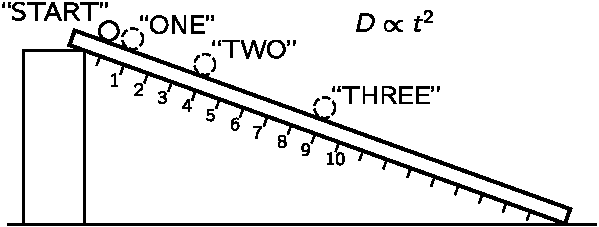
\includegraphics[width=0.8\linewidth]{fyz_fig064.pdf}
      \caption{Zatížená tyč podepřená na jednom konci (\cite[s.~64]{Feynman01})}
      \label{fyz:fig064}
    \end{figure}
    
    Způsob měření vzdálenosti byl dobře znám dávno před Galileem, neexistovaly však přesné způsoby 
    měření času, zejména krátkých časů. Ačkoli sám později vynalezl spolehlivější hodiny (ne však 
    takové, jaké známe dnes), prováděl Galileo své první experimenty tak, že pomocí vlastního 
    pulzu určoval stejné časové intervaly. Udělejme nyní totéž:
    
    Počítejme údery tepu po dobu pohybu kuličky: „raz... dva... tři... čtyři... pět... šest... 
    sedm... osm...“. Požádejme kolegu, aby označil polohu kuličky při každém tepu. Tak můžeme 
    \emph{změřit vzdálenost}, kterou kulička urazila od vypuštění za jeden, dva, tři atd. stejné 
    intervaly času. Galileo vyjádřil výsledek svých pozorování následujícím způsobem: Když si 
    polohu kuličky značíme po \num{1}, \num{2}, \num{3}, \num{4} ... jednotkách času od jejího 
    vypuštění, pak jsou tyto značky vzdáleny od počátečního bodu úměrně číslům \num{1}, \num{4}, 
    \num{9}, \num{16} ... Dnes bychom řekli, že vzdálenost je úměrná druhé mocnině času
    \begin{equation*}
      s \sim t^2.
    \end{equation*}
    
    Studium \emph{pohybu}, které je základem všech fyzikálních disciplín, se zabývá dvěma otázkami: 
    kde? a kdy?
    
  \section{Čas}
    Nejprve se zamysleme nad tím, co chápeme jako \emph{čas}. Co \emph{je} čas? Bylo by krásné, 
    kdyby se nám podařilo najít dobrou definici času. Ve slovnících nacházíme „čas“ definovaný jako 
    „období“ a „období“ zase jako „čas“, což se nezdá být příliš použitelné. Snad bychom mohli 
    říci: „Čas je to, co se děje, když se nic jiného neděje.“ To nás však nedovede příliš daleko. 
    Je snad právě tak dobré, když si přiznáme, že čas je jedna z těch věcí, kterou pravděpodobně 
    nemůžeme definovat (v slovníkovém smyslu), a říkat o něm jen to, co už víme: Čas je to, jak 
    dlouho čekáme!
    
    Skutečně důležité však není to, jak čas \emph{definujeme}, ale jak ho \emph{měříme}. Jedním ze 
    způsobů měření časuje využití něčeho, co se neustále děje, a to pravidelným způsobem - něčeho, 
    co je \emph{periodické}. Například den. Den, ten se stále opakuje. Když však o tom uvažujeme, 
    můžeme si položit otázku: .Jsou dny periodické, jsou pravidelné? Mají všechny dny stejnou 
    délku?“ Určitě máme dojem, že letní dny jsou delší než zimní. Ovšem, když se moc nudíme, 
    připadají nám i některé zimní dny velmi dlouhé. Již jsme určitě slyšeli někoho zvolat: „Ach, to 
    byl dnes dlouhý den!“
    
    Zdá se však, že dny jsou v \emph{průměru} téměř stejně dlouhé. Existuje způsob, jak prověřit, 
    jsou-li dny stejně dlouhé, buď dva za sebou následující nebo alespoň v průměru? Jedním ze 
    způsobů je porovnání s jiným periodickým jevem. Všimněme si, jak je možné takové porovnání 
    provést pomocí přesýpacích hodin. Pomocí přesýpacích hodin „vytvoříme“ periodičnost, budeme-li 
    je ve dne v noci překlápět, jakmile se přesype poslední zrnko písku.
    
    Potom nám stačí spočítat počet překlopení hodin od jednoho do druhého rána. Tak zjistíme, že 
    počet „hodin“, tj. překlopení, není každý „den“ stejný! Mohli bychom podezřívat Slunce nebo 
    přesýpací hodiny nebo oboje. Po jistých úvahách by nás mohlo napadnout, že „hodiny“ je třeba 
    počítat od poledne do poledne. (Poledne tu \emph{nedefinujeme} jako 12.00 hodin, ale jako 
    okamžik, kdy Slunce vrcholí.) Tentokrát bychom zjistili, že každý den má stejný počet „hodin“. 
    Získali jsme jakousi důvěru, že jak „hodina“, tak „den“ se pravidelně opakují, tj. vyznačují po 
    sobě následující stejné časové intervaly, ačkoli jsme \emph{nedokázali}, že jsou „skutečně“ 
    periodické. Je možné si položit otázku, zda by nemohla jakási zázračná bytost zpomalovat pohyb 
    písku v noci a urychlovat ho ve dne. Náš experiment na takovouto otázku odpověď nedává. Můžeme 
    říci jen tolik, že jsme zjistili, že pravidelnost jednoho druhu je ve shodě s pravidelností 
    jiného druhu. Můžeme říci, že naše definice času spočívá v opakování se určité zřejmě  
    periodické události.
    
  \section{Krátké časy}
    Měli bychom si uvědomit, že při zkoušce opakování dne jsme získali i další důležitý poznatek. 
    Našli jsme způsob přesnějšího měření \emph{částí} dne. Našli jsme způsob měření kratších 
    časových úseků. Můžeme v tomto postupu pokračovat a tak měřit ještě kratší časové intervaly?
    Galileo zjistil, že kyvadlo vykoná každý kyv za stejnou dobu, zůstává-li velikost rozkyvu malá. 
    Potvrzuje to test určující počet kyvů kyvadla za jednu „hodinu“. Takto můžeme vytvořit značky 
    zlomků hodiny. Použijeme-li mechanické zařízení na počítání kyvů a na udržení chodu kyvadla - 
    získáme kyvadlové hodiny našich dědečků.
    
    Dohodněme se, že jestliže naše kyvadlo kmitá \num{3600}-krát za hodinu (a je-li takových hodin 
    \num{24} za den), nazveme periodu kyvadla jednou „sekundou“. Tak jsme naši původní časovou 
    jednotku rozdělili přibližně na \num{10e5} částí. Stejně můžeme sekundu rozdělit na menší a 
    menší intervaly. Zjistíme, že není praktické konstruovat mechanická kyvadla, která kývají 
    libovolně rychle, ale můžeme konstruovat \emph{elektrická} kyvadla, nazývaná 
    \textbf{oscilátory}, která nám poskytnou periodicitu s velmi krátkými periodami kmitů. V 
    takových elektronických oscilátorech je to elektrický proud, který kmitá podobným způsobem jako 
    kyvadlo.
    
    Můžeme sestrojit celou řadu takových elektronických oscilátorů, každý s periodou desetkrát 
    kratší, než má předcházející. Každý oscilátor můžeme „kalibrovat“ vůči sousednímu pomalejšímu 
    oscilátoru určením počtu kmitů,jež vykoná za dobu jednoho kmitu pomalejšího oscilátoru. Je-li 
    perioda kmitů našich hodin kratší než zlomek sekundy, nemůžeme určovat kmity bez pomocného 
    zařízení, které rozšiřuje naši pozorovací schopnost. Jedním z takových zařízení je 
    \emph{osciloskop} s elektronovým paprskem, jenž pracuje jako jakýsi mikroskop pro krátké časy. 
    Toto zařízení zakresluje na fluorescenční stínítko graf elektrického proudu (nebo napětí) v 
    závislosti na čase. Připojíme-li osciloskop ke dvěma sousedním oscilátorům z naší posloupnosti 
    tak, že nejprve zakresluje proud jednoho a potom proud druhého oscilátoru, dostáváme dva grafy 
    podobné těm, které jsou znázorněny na obr. \ref{fyz:fig065}. Tak můžeme pohotově určit počet 
    period rychlejšího oscilátoru po dobu jedné periody pomalejšího oscilátoru. Obr. 
    \ref{fyz:fig065} Dva pohledy na obrazovku osciloskopu
    \begin{figure}[ht!]  %\ref{fyz:fig065}
      \centering
      \begin{tabular}{cc}
        \subfloat[ ]{\label{fyz:fig065a}
          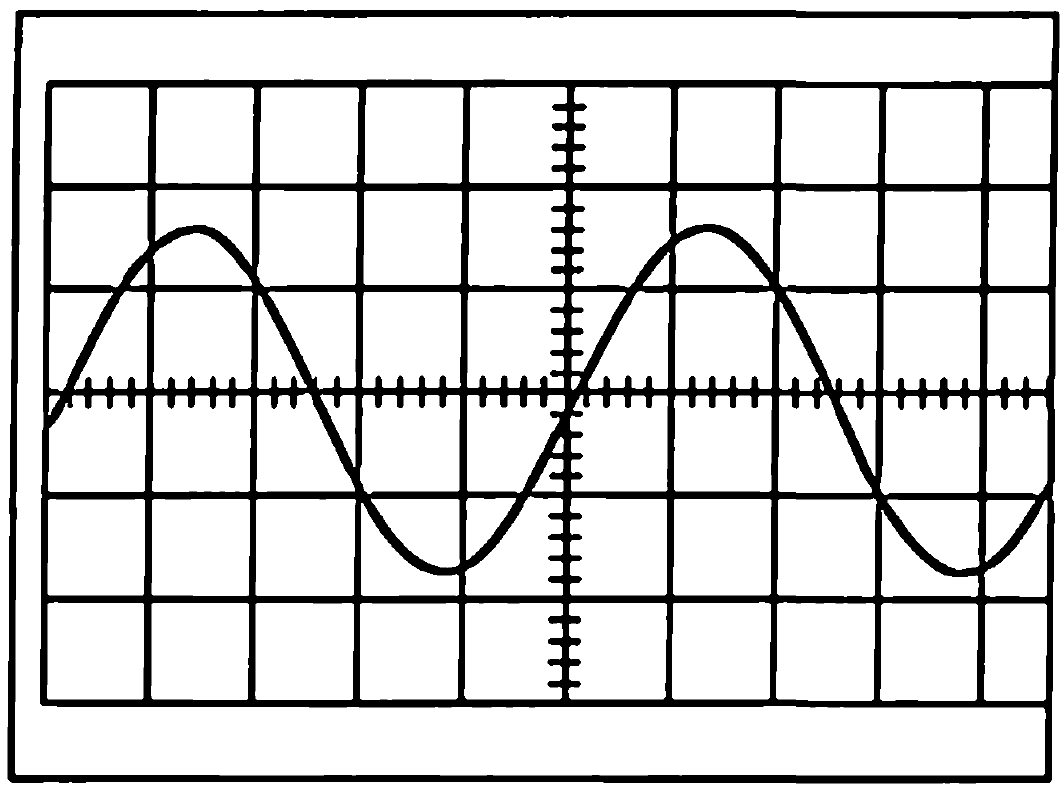
\includegraphics[width=0.2\textwidth]{fyz_fig065a.png}}
        \hspace{0.1\linewidth}                                                       &
        \subfloat[ ]{\label{fyz:fig065b}
          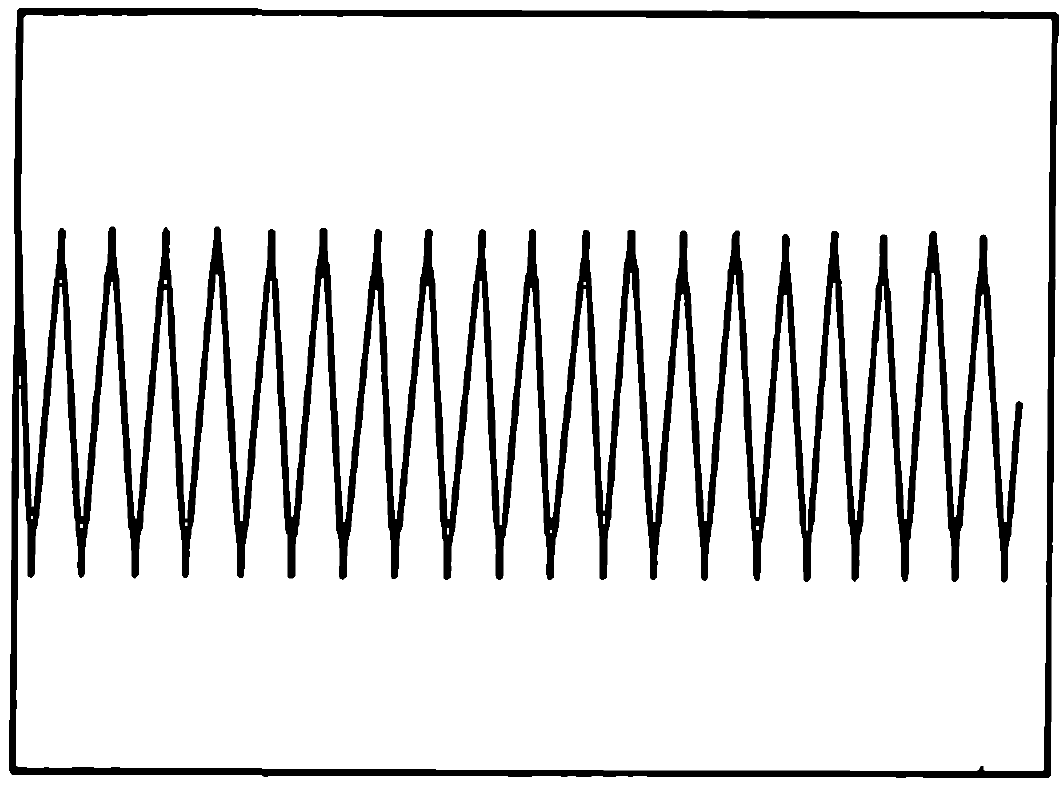
\includegraphics[width=0.2\textwidth]{fyz_fig065b.png}}
      \end{tabular}
      \caption{a) osciloskop je připojen k jednomu oscilátoru. b) osciloskop je připojen k 
               oscilátoru, jehož perioda je desetinou periody předcházejí oscilátoru 	
               (\cite[s.~66]{Feynman01})}
      \label{fyz:fig065}
    \end{figure}
    
    Pomocí moderních elektronických metod byly zkonstruovány oscilátory s periodou krátkou kolem 
    \num{10e12} sekund a byly kalibrovány (porovnávacími metodami podobnými metodě, kterou
    jsme popsali) v naší standardní časové jednotce - sekundě. Vynalezení a zdokonalení „laseru“ 
    neboli zesilovače světla umožnilo v nedávných letech konstrukci oscilátorů s ještě kratšími 
    periodami než \num{10e-12} sekundy, ale zatím je nebylo možné kalibrovat popsaným způsobem, 
    ačkoli i k tomu nepochybně dojde.
    
    Časy kratší než \num{10e-12} sekundy byly měřeny, ale jinými způsoby. Ve skutečnosti byla 
    použita jiná \emph{definice} „času“. Jedním ze způsobů bylo pozorování mezi dvěma událostmi, 
    jež se stanou s pohybujícím se předmětem. Jestliže například zapneme a pak vypneme reflektory 
    pohybujícího se auta, můžeme určit, jak \emph{dlouho} byla světla zapnutá, jestliže víme, 
    \emph{kde} byla zapnuta a vypnuta a jakou rychlostí se auto pohybovalo. Čas určíme tak, že 
    vzdálenost, po kterou byla světla zapnutá, dělíme rychlostí.
    
    Nedávno byla taková metoda použita pro měření doby života \(\pi^0\) mezonu. Mikroskopickým 
    pozorováním drobných stop zanechaných ve fotografické emulzi, v níž byl mezon vytvořen, se 
    zjistilo, že \(\pi^0\) mezon (pohybující se rychlostí téměř rovnou rychlostí světla) urazil v 
    průměru vzdálenost \num{10e-7} metrů dříve, než se rozpadl. Žil jen přibližně \num{10e-16} 
    sekundy. Je třeba však zdůraznit, že jsme použili trochu jinou definici „času“ než předtím. 
    Dokud však není rozpor v našem chápání, věříme, že tyto definice jsou dostatečně rovnocenné.
    
    Dalším rozšířením našich metod - a je-li to nevyhnutelné i našich definicí - můžeme určit 
    trvání ještě rychlejších fyzikálních jevů. Můžeme hovořit o periodě jaderných kmitů. Můžeme 
    hovořit o délce života nově objevených podivných rezonancí (částic). Jejich celková délka 
    života je pouze \num{10e-24} sekundy, což je přibližně doba, kterou potřebuje světlo 
    (pohybující se největší ze známých rychlostí) k průchodu jádrem vodíku (což je 
    nejmenší známý předmět).
    
    Co je možné říci o ještě kratších časech? Existuje čas v ještě menším měřítku? Má vůbec smysl 
    hovořit o ještě kratších časech, když neumíme měřit - nebo dokonce si rozumně představit - 
    něco, co se odehrává v kratším čase? Snad ne. Toto jsou některé otevřené otázky, které si 
    budeme klást a na které snad nalezneme odpověď za dalších dvacet nebo třicet let.
    
  \section{Dlouhé časy}
    Nyní uvažujme časy delší než jeden den. Měření dlouhých časů je jednoduché; budeme prostě 
    počítat dny - dokud bude existovat někdo, kdo to bude moci dělat. Tak docházíme k další 
    přirozené periodicitě: roku, který má přibližně \num{365} dní. Zjišťujeme i to, příroda nám 
    někdy poskytuje počítadlo let, a to v podobě letokruhů stromů nebo říčních naplavenin. V 
    některých případech můžeme využít těchto přírodních časových značek k určení času, který 
    uplynul od nějaké dávné události.
    
    Nemůžeme-li při měření dlouhých časů počítat roky, musíme hledat jiný způsob měření. Jedním z 
    nejúspěšnějších je použití \emph{radioaktivního materiálu} jako „hodin“. V tomto případě nemáme 
    periodický proces tak jako v případě dne nebo kyvadla, ale máme nový druh „pravidelností“. 
    Zjišťujeme, že radioaktivita jistého vzorku materiálu klesá o stejné \emph{procento},    
    jestliže ji určujeme ve dvou stejných po sobě jdoucích přírůstcích jeho věku. Nakreslíme-li 
    graf radioaktivity v závislostí na čase (měřeného např. ve dnech), dostaneme křivku jako na 
    obr. \ref{fyz:fig066}. Vidíme, že v případě poklesu radioaktivity na jednu polovinu za \(T\) 
    dní (\(T\) nazýváme „poločasem rozpadu“) dochází k poklesu na jednu čtvrtinu za dalších \(T\) 
    dní atd. V libovolném časovém intervalu \(t\) je obsaženo \(t/T\) „poločasů rozpadu“ a podíl 
    aktivity, která zbývá po čase \(t\) je roven \((l/2)^{\frac{t}{T}}\).

    \begin{figure}[ht!]  %\ref{fyz:fig066}
      \centering
      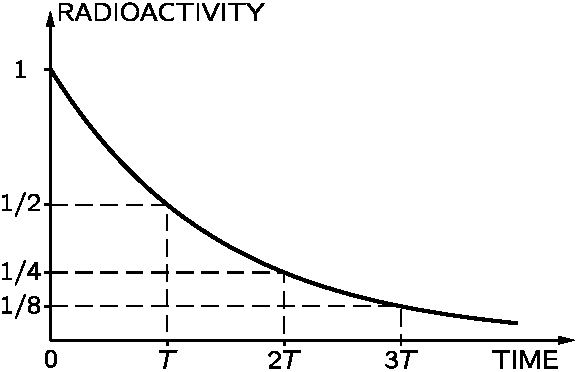
\includegraphics[width=0.6\linewidth]{fyz_fig066.pdf}
      \caption{Pokles radioaktivity s časem; aktivita klesne o polovinu za dobu \uv{poločasu 
      rozpadu} (\cite[s.~68]{Feynman01})}
      \label{fyz:fig066}
    \end{figure}    
    Víme-li, že kousek materiálu, například dřeva, obsahoval při svém vzniku množství \(A\) 
    radioaktivního materiálu a přímým měřením zjistíme, že nyní obsahuje množství \(B\), můžeme 
    vypočítat věk předmětu \(t\) řešením rovnice
    \begin{equation}\label{FYZ:eq065}
      \left(\dfrac{1}{2}\right)^{\dfrac{t}{T}} = \dfrac{B}{A}
    \end{equation}
    
    Naštěstí existují případy, v nichž známe množství radioaktivity přítomné při vzniku předmětu. 
    Víme například, že oxid uhličitý ve vzduchu obsahuje malý zlomek radioaktivního izotopu uhlíku 
    \ce{^{14}C} (neustále doplňovaný působením kosmického záření). Když měříme \emph{celkový} obsah 
    uhlíku v předmětu, víme, že určitý zlomek tohoto množství byl původně radioaktivní \ce{^{14}C}, 
    a proto známe počáteční množství \(A\) vystupující v uvedeném vztahu. Uhlík \ce{^{14}C} má 
    poločas rozpadu \num{5000} let. Pečlivým měřením můžeme zjistit množství, které zůstalo po 
    \num{20} poločasech rozpadu nebo jiném podobném čase a můžeme proto stanovit stáří předmětů z 
    organických látek, které rostly už před \num{100000} lety.
    
    Zajímá nás však i věk ještě starších věcí a zdá se, že ho umíme určit. Mnohé z našich poznatků 
    jsou založeny na měření jiných radioaktivních izotopů, jež mají různé poločasy rozpadu. 
    Použijeme-li izotop, jenž má delší poločas rozpadu, můžeme měřit delší časy. Například uran má 
    izotop, jehož poločas rozpadu je asi \num{10e9} let, takže když nějaký materiál při svém 
    vytvoření před \num{10e9} lety obsahoval uran, zůstane dnes z tohoto uranu jen polovina. Uran 
    se při rozpadu mění na olovo. Uvažujme kousek horniny, jenž vznikl před mnoha lety nějakým 
    chemickým procesem. Olovo, jež se chemicky liší od uranu, by mělo být v jedné části horniny a 
    uran v jiné části horniny. Uran a olovo jsou tedy při vzniku horniny odděleny. Jestliže však 
    tentýž kousek horniny zkoumáme dnes, pak na místě, kde byl původně uran, najdeme určitou část 
    uranu a určitou část olova. Porovnáním těchto částí můžeme určit, kolik procent uranu zaniklo a 
    přeměnilo se na olovo. Touto metodou bylo stáří některých hornin určeno na několik miliard let. 
    Zobecněním této metody, kdy místo v horninách byly uran a olovo sledovány v mořích a byly 
    uvažovány celosvětové průměry, se podařilo (v průběhu nedávných let) určit stáří Země na 
    přibližně \num{5.5} miliardy let.
    
    Povzbuzující je zjištění, že podle uranové metody je Země stejně stará jako meteority, které na 
    ni dopadají. Vypadá to tedy tak, že Země byla vytvořena z kusů skal létajících prostorem a 
    meteority jsou pravděpodobně zbytky tohoto materiálu. Někdy před více než pěti miliardami let 
    měl vesmír svůj počátek. Dnes se domníváme, že alespoň část vesmíru měla počátek před deseti 
    nebo dvanácti miliardami let. Nevíme, co se stalo předtím. Mohli bychom se vlastně ptát: „Má 
    taková otázka smysl? Má dávno minulý čas vůbec nějaký smysl?“
    
    \begin{figure}[ht!]  %\ref{fyz:fig075}
      \centering
      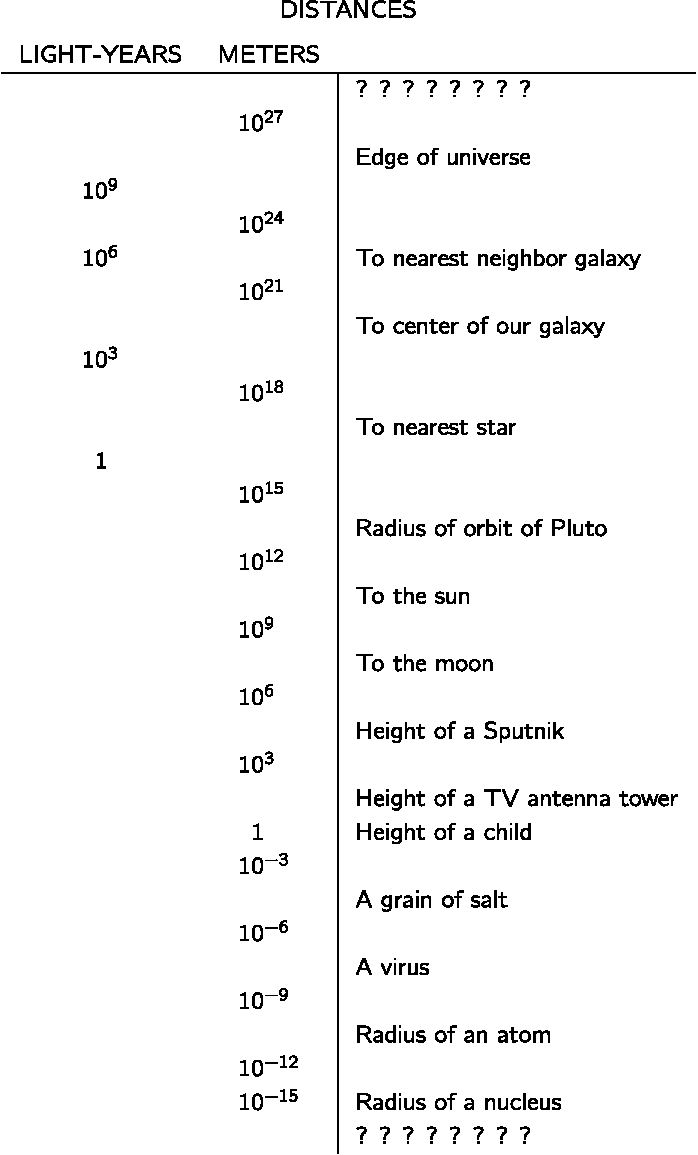
\includegraphics[width=0.7\linewidth]{fyz_fig075.pdf}
      \caption{Tabulka časů (\cite[s.~69]{Feynman01})}
      \label{fyz:fig075}
    \end{figure}

  \section{Jednotky a standardy času}
    Již jsme naznačili, že je vhodné vycházet z nějaké standardní časové jednotky a ostatní časy 
    vztahovat k jejím násobkům nebo zlomkům. Co máme vzít jako základní standard času? Máme za něho 
    zvolit tep lidského srdce? Porovnáme-li tepy, zjistíme, že se značně liší. Porovnáním dvou 
    hodin zjistíme, že se jejich údaje tak mnoho neliší. Proto by bylo možné vzít za standard 
    hodiny. Jenže čí hodiny. Existuje pohádka o švýcarském chlapci, který chtěl, aby všechny hodiny 
    v jeho městě zvonily poledne ve stejnou chvíli. Tak se vydal na cestu, aby přesvědčil lidi o 
    užitečnosti této myšlenky. Každý vlastník hodin považoval tuto myšlenku za vynikající, ale jen 
    v případě, kdy by se všechny ostatní hodiny přizpůsobily jeho hodinám. Je dost těžké 
    rozhodnout, které hodiny je třeba vzít za standard. Naštěstí všichni uznáváme jedny hodiny - 
    Zemi. Perioda otáčení Země byla dlouho považována za časový standard. Když však byla měření 
    stále přesnější, zjistilo se, že rotace Země není dokonale periodická, měříme-li ji 
    nejpřesnějšími hodinami. Těmi „nejpřesnějšími“ hodinami jsou ty, jejichž přesnosti důvěřujeme 
    proto, že jejich údaje navzájem souhlasí. Dnes víme, že z různých důvodů jsou některé dny 
    kratší, jiné delší a v průměru se s postupem času perioda otáčení Země trochu prodlužuje.
    
    Až donedávna jsme nenašli nic lepšího, než periodu zemské rotace, takže všechny hodiny se 
    vztahovaly k délce dne a sekunda byla definována jako \(\frac{1}{\num{86400}}\) středního 
    slunečního dne. Nedávno jsme však získali zkušenosti s některými přírodními oscilátory, o nichž 
    dnes předpokládáme, že poskytují stálejší časový normál než Země a jsou také založeny na 
    přírodním jevu přístupném všem. Jsou to tzv. „atomové hodiny“. Jejich základní vnitřní periodou 
    je perioda atomových kmitů, jež téměř nezávisí na teplotě a jiných vnějších vlivech. Tyto 
    hodiny měří čas s přesností lepší než \num{10e-9}.
    
    Protože se podařilo sestrojit hodiny, udávající čas mnohem přesněji než astronomické metody, 
    je dnes sekunda definována Jako doba trvání \num{9192631770} period záření, které odpovídá 
    přechodu mezí dvěma hladinami velmi jemné struktury základního stavu atomu cesia \num{133}.
    
  \section{Velké vzdálenosti}
    Nyní věnujme pozornost otázce \emph{vzdáleností}. Jak vzdálené, nebo jak velké jsou věci? Každý 
    ví, že při měření vzdáleností vezmeme tyč, postupně ji přikládáme a počítáme. Nebo si pomůžeme 
    palcem a počítáme. Začneme tedy s jednotkou a počítáme. Jak se však měří menší věci? Jak 
    rozdělujeme vzdálenosti? Stejně tak jako jsme rozdělovali čas: Vezmeme menší jednotku a 
    počítáme, kolik takových jednotek vytvoří větší jednotku. Tak můžeme měřit menší a ještě menší 
    délky.

    \begin{figure}[ht!]  %\ref{fyz:fig068}
      \centering
      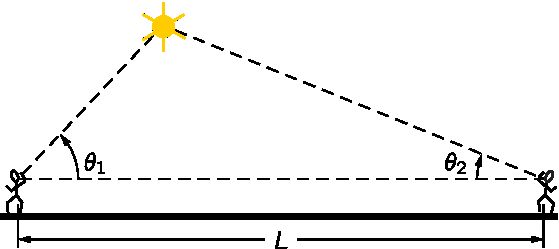
\includegraphics[width=0.6\linewidth]{fyz_fig068.pdf}
      \caption{Výška družice určená triangulací (\cite[s.~70]{Feynman01})}
      \label{fyz:fig068}
    \end{figure}
    
    Vzdáleností však nerozumíme vždy to, co můžeme měřit metrovou tyčí. Bylo by těžké měřit 
    horizontální vzdálenost mezi dvěma vrcholy hor jen pomocí dřevěného metru. Ze zkušeností víme, 
    že vzdálenost je možné měřit i jiným způsobem - \textbf{triangulací}. To sice znamená použít 
    jinou definici vzdálenosti, ale v případech, kdy jsou obě dvě definice použitelné, dávají 
    shodný výsledek. Prostor je více méně tím, za co ho považoval Euklides, a proto jsou uvedené 
    definice shodné. Protože jsou shodné na Zemi, máme k triangulaci určitou důvěru i při použití 
    pro ještě větší vzdálenosti. Například pomocí triangulace jsme mohli změřit výšku první umělé 
    družice. Zjistili jsme, že byla asi \num{5e5} metrů vysoko. Při pečlivém měření můžeme podobně 
    změřit vzdálenost k Měsíci. Dva teleskopy na různých místech Země nám poskytnou dva úhly, které 
    potřebujeme. Takto se zjistilo, že Měsíc je od Země vzdálen \num{4e8} metrů.
    
    Tímto způsobem však nemůžeme měřit vzdálenost ke Slunci, nebo alespoň dosud se to ještě nikomu 
    nepodařilo. Přesnost zaostření na daný bod na Slunci a měření uhlů není dostatečná pro určení 
    vzdálenosti ke Slunci. Jak tedy můžeme měřit vzdálenost ke Slunci? Musíme vymyslet zobecnění 
    myšlenky triangulace. Měříme relativní vzdálenosti všech planet astronomickými pozorováními 
    míst, kde planety vidíme, a tak dostáváme obraz sluneční soustavy se správnými 
    \emph{relativními} vzdálenostmi, ale bez \emph{absolutní} vzdálenosti. Potom potřebujeme jedno 
    absolutní měření, což lze provést různými způsoby. Jedním ze způsobů, o němž se až donedávna 
    předpokládalo, že je nejpřesnější, je měření vzdálenosti od Země k Erosu, jedné z malých 
    planetek, jež se čas od času pohybují v blízkosti Země. Triangulací na tento malý objekt je 
    možné získat požadované cejchovací měření. Známe-li ostatní relativní vzdálenosti, můžeme určit 
    například vzdálenost od Země ke Slunci nebo od Země k Plutu.
    
    \begin{figure}[ht!]  %\ref{fyz:fig069}
      \centering
      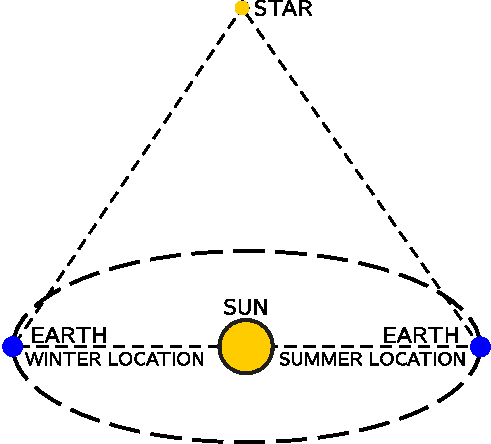
\includegraphics[width=0.7\linewidth]{fyz_fig069.pdf}
      \caption{Vzdálenost blízkých hvězd je možné změřit triangulací, když se jako základny použije 
               průměr zemské oběžné dráhy. (\cite[s.~71]{Feynman01})}
      \label{fyz:fig069}
    \end{figure}     
    V posledních letech se velmi zdokonalily naše poznatky o rozměrech sluneční soustavy. V 
    laboratořích firmy Jet Propulsion byla přesně změřena vzdálenost od Země k Venuši přímým 
    radarovým pozorováním. To je, samozřejmě, další způsob určování vzdáleností. Známe rychlost, 
    jakou se šíří světlo (a tedy i radarové vlny) a předpokládáme, že ta rychlost je stejná všude 
    mezi Zemí a Venuší. Vyšleme rádiovou vlnu a měříme čas, dokud se odražená vlna nevrátí zpět. Z 
    \emph{času} odvodíme \emph{vzdálenost} za předpokladu, že známe rychlost. Máme tedy skutečně 
    jinou definici měření vzdálenosti.
    
    Jak měříme vzdálenost k hvězdě, která je mnohem dále? Naštěstí se můžeme vrátit k triangulační 
    metodě, neboť Země nám při svém pohybu kolem Slunce poskytuje velkou základnu pro měření 
    předmětů mimo sluneční soustavu. Zaostříme-li teleskop na hvězdu v létě a v zimě, máme naději 
    určit dva potřebné úhly dostatečně přesně a můžeme změřit vzdálenost k hvězdě.
   
    Co je však možné dělat tehdy, když jsou hvězdy příliš vzdáleny pro použití triangulace? 
    Astronomové vždy objevují nové způsoby měření vzdáleností. Zjistili například, že je možné 
    odhadnout velikost a jasnost\footnote{V astronomii se pozorovaná jasnost hvězdy udává jako její 
    hvězdná velikost (magnituda).} hvězdy pomocí její barvy. Byly měřeny barva a jasnost mnoha 
    blízkých hvězd - jejichž vzdálenosti známe pomocí triangulace - a bylo zjištěno, že existuje 
    jednoznačný vztah mezi barvou a vlastní jasností hvězd (ve většině případů). Změříme-li barvu 
    vzdálené hvězdy, můžeme využít tohoto vztahu a určit vlastní jasnost hvězdy. Měřením jasnosti 
    hvězdy, kterou \emph{pozorujeme} na Zemi (mohli bychom říci, jak tmavá se nám hvězda jeví), 
    můžeme vypočítat, jak je hvězda vzdálená. (Při dané vlastní jasnosti klesá pozorovaná jasnost 
    se čtvercem vzdálenosti.) Pěkným potvrzením správnosti této metody měření hvězdných vzdáleností 
    jsou výsledky získané pro skupinu hvězd známých jako kulové hvězdokupy. Fotografie takové 
    skupiny je znázorněna na obr. \ref{fyz:fig070}. Hned při prvním pohledu na fotografuje člověk 
    přesvědčen, že tyto hvězdy jsou pohromadě. Tentýž výsledek je možné získat i z měření 
    vzdáleností pomocí metody jasnost-barva.

    \begin{figure}[ht!]  %\ref{fyz:fig070}
      \centering
      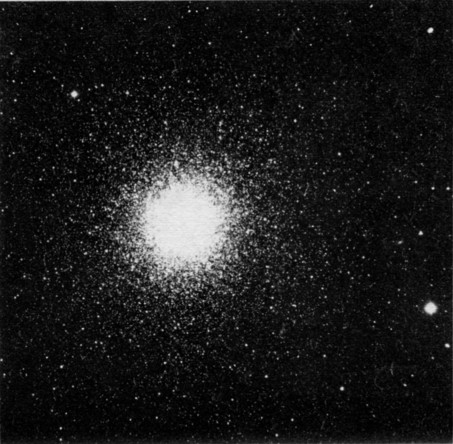
\includegraphics[width=0.6\linewidth]{fyz_fig070.jpg}
      \caption{Hvězdokupa v blízkosti centra naší galaxie. Tyto hvězdy jsou od Země vzdáleny 
               \num{30000} světelných let, tedy asi \SI{3e20}{\m}. (\cite[s.~72]{Feynman01})}
      \label{fyz:fig070}
    \end{figure}
    
    Studium mnoha kulových hvězdokup poskytuje další důležitou informaci. Bylo zjištěno, že v 
    určité části oblohy je vysoká koncentrace takových shluků a většina z nich je od náš téměř 
    stejné vzdálena. Spojením této informace s jinými důkazy docházíme k závěru, že tato 
    koncentrace hvězdokup označuje střed naší galaxie. Tak víme, že vzdálenost do středu galaxie je 
    asi \num{e20} metrů. 
    

    \begin{figure}[ht!]  %\ref{fyz:fig071}
      \centering
      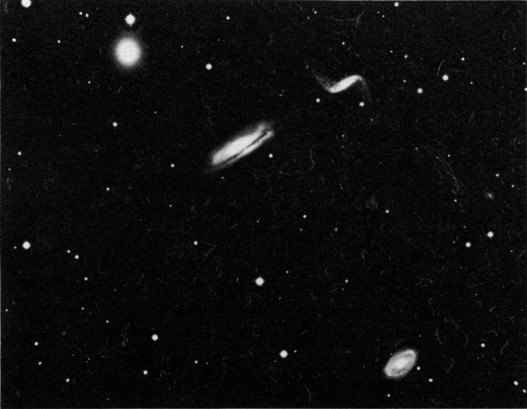
\includegraphics[width=0.6\linewidth]{fyz_fig071.jpg}
      \caption{Spirální galaxie podobná naší. Za předpokladu, že její průměr je stejný jako průměr 
               naší galaxie, můžeme z její zdánlivé velikosti určit její vzdálenost. Od Země je 
               vzdálena \num{30} milionů světelných roků (\(\SI{3e23}{\m}\)). 
               (\cite[s.~72]{Feynman01})}
      \label{fyz:fig071}
    \end{figure}

    Poznání velikosti naší vlastní galaxie nám dalo do ruky klíč k měření ještě větších vzdáleností 
    - vzdáleností k jiným galaxiím. Obr. \ref{fyz:fig071} je fotografie galaxie, jež má tvar velmi 
    podobný naší galaxii. Pravděpodobně je i stejně velká. (Jiné důkazy hovoří ve prospěch 
    myšlenky, že všechny galaxie jsou přibližně stejně velké.) Je-li stejně velká jako naše 
    Galaxie, pak můžeme určit její vzdálenost. Změříme úhel, který vytíná na obloze a když zjistíme 
    její průměr, vypočteme její vzdálenost opět triangulací.

    \begin{figure}[ht!]  %\ref{fyz:fig072}
      \centering
      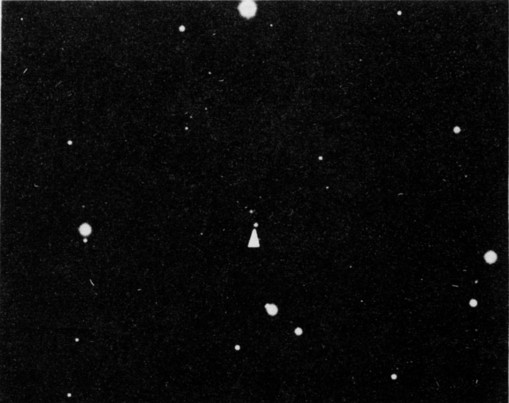
\includegraphics[width=0.6\linewidth]{fyz_fig072.jpg}
      \caption{Od nás nejvzdálenější objekt 3C295 v souhvězdí pastýře (označený šipkou), jenž byl v 
               roce \num{1960} změřen \num{5} metrovým teleskopem (\cite[s.~73]{Feynman01})}
      \label{fyz:fig072}
    \end{figure}
    
    Pomocí obrovského teleskopu na Mt. Palomar byly nedávno získány fotografie velmi vzdálených 
    galaxií. Jedna z nich je na obr. \ref{fyz:fig072}. Dnes se domníváme, že některé z těchto 
    galaxií jsou v přibližně poloviční vzdálenosti k hranicím vesmíru - vzdáleny \num{e26} metrů, 
    což je největší vzdálenost, kterou můžeme uvažovat!
    
  \section{Malé vzdálenosti}
    Uvažujme nyní menší vzdálenosti. Dělení metru na části je jednoduché. Bez větších problémů 
    můžeme vyznačit tisíc stejných částí, které dohromady dávají jeden metr. S trochu většími 
    obtížemi, ale podobným způsobem (pomocí dobrého mikroskopu), můžeme vyznačit tisíc stejných 
    částí milimetru a vytvořit tak stupnici mikrometrů (miliontin metru). Je těžké pokračovat k 
    menším stupnicím, protože nemůžeme \uv{vidět} předměty, jež jsou menší než vlnová délka 
    viditelného světla (kolem \num{5e-7} metru).

    \begin{figure}[ht!]  %\ref{fyz:fig073}
      \centering
      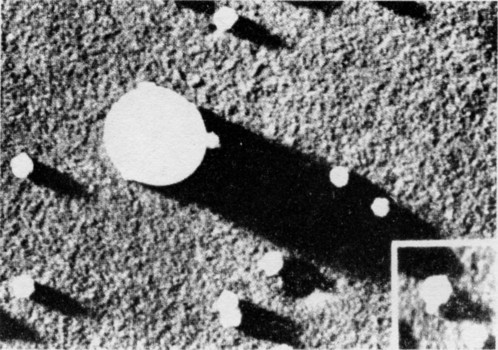
\includegraphics[width=0.6\linewidth]{fyz_fig073.jpg}
      \caption{Fotografie virových molekul zhotovená pomocí elektronového mikroskopu. \uv{Velká} 
               koule slouží ke kalibraci a má průměr \SI{2e-7}{\m}  (\cite[s.~74]{Feynman01})}
      \label{fyz:fig073}
    \end{figure}
    
    Omezovat se jen a to, co můžeme vidět, však není  nevyhnutelné. Pomocí elektronového mikroskopu 
    můžeme pokračovat v našem postupu a můžeme získat fotografie v ještě menším měřítku, asi tak 
    \num{e-8} metru  (\ref{fyz:fig073}). Nepřímými měřeními - jistým druhem triangulace v 
    mikroskopických rozměrech - můžeme pokračovat v měření menších a menších předmětů. Především ze 
    způsobu odrazu světla krátkých vlnových délek (rentgenových paprsků) na systému bodů se známými 
    rozestupy určíme vlnovou délku světelného vlnění. Potom z rozptylových obrazců téhož světla na 
    krystalu můžeme určit relativní polohy atomů v krystalu. Tak získáme výsledky, jež souhlasí s 
    rozložením atomů určeným chemickými prostředky. Tímto způsobem zjistíme, že atom má průměr asi 
    \num{e-10} metru. 

    Mezi typickým atomovým rozměrem \num{e-10} metru a jadernými rozměry \num{e-15} metru řádově 
    \num{e5}-krát menšími je velká \uv{mezera} ve fyzikálních rozměrech. Pro jaderné rozměry se 
    stává výhodným jiný způsob měření velikosti. Měříme \emph{zdánlivou} plochu \(\sigma\) 
    nazývanou \emph{účinným průřezem}. Chceme-li zjistit poloměr, získáme ho ze vztahu \(\sigma = 
    \pi r^2\), neboť jádro je téměř kulové. 

    Jaderný průřez je možné měřit při dopadu svazku vysokoenergetických částic na tenkou vrstvu 
    materiálu sledováním počtu částic jež jsou odchýleny. Tyto vysokoenergetické částice  proniknou 
    řídkým oblakem elektronů a zastaví se nebo se vychýlí jen tehdy, narazí-li na soustředěnou 
    hmotu jádra. Předpokládejme, že máme kousek materiálu, který je \SI{1}{\cm} tlustý. V takovém 
    kousku bude asi \num{e8} atomových vrstev. Jádra jsou však tak malá, že je málo pravděpodobné, 
    že se dvě jádra ocitnou za sebou. Můžeme si tedy \emph{představit} že velmi zvětšený pohled na 
    situaci - hledíme-li ve směru svazku částic - vypadá tak jako na obr. \ref{fyz:fig076}. 

    \begin{figure}[ht!]  %\ref{fyz:fig076}
      \centering
      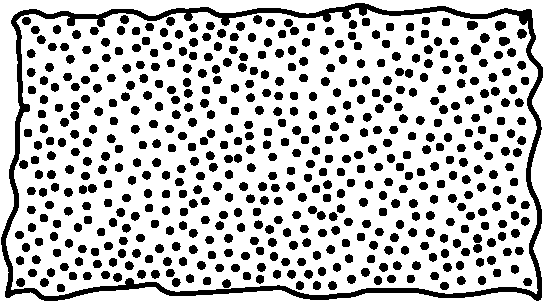
\includegraphics[width=0.7\linewidth]{fyz_fig076.pdf}
      \caption{Vzdálenost blízkých hvězd je možné změřit triangulací, když se jako základny použije 
               průměr zemské oběžné dráhy. (\cite[s.~71]{Feynman01})}
      \label{fyz:fig076}
    \end{figure}   
    Pravděpodobnost, že velmi malá částice se na své cestě destičkou srazí s jádrem, je dána 
    podílem celkové plochu jader a celkové plochy vzorku. Předpokládejme, že na ploše \(A\) našeho 
    kousku materiálu se nachází \(N\) atomů (samozřejmě, každý s jedním jádrem). Pak celková plocha 
    \uv{pokrytá} jádry je rovna \(N\sigma\). Nechť je počet částic svazku, jež dopadají na kousek 
    materiálu roven \(n_1\) a počet částic, jež na druhé straně z materiálu vycházejí, roven 
    \(n_2\). Zlomek těch, které neprojdou materiálem, je \(\frac{n_1-n_2}{n_1}\) a měl by být roven 
    poměru \(N\frac{\sigma}{A}\) plochy pokryté jádry a původní plochy \(A\). Poloměr jádra můžeme 
    dostat z rovnice
    \begin{equation}\label{FYZ:eq066}
      \pi r^2 = \sigma = \frac{A}{N}\cdot\frac{n_1-n_2}{n_1}.
    \end{equation}
    (Tato rovnice je správná jen tehdy, když je plocha pokrytá jádry jen malou částí celkové 
    plochy, tj. když \(\frac{n_1-n_2}{n_1}\) je mnohem menší než \num{1}. V opačném případě je 
    potřebná korekce, která bere v úvahu skutečnost, že některé jádra budou částečně zastíněna 
    jádry stojícími před nimi.) Podobnými experimenty se podařilo zjistit, že poloměr jádra je od 
    \SI{1e-15}{\m} do \SI{6e-15}{\m}. Na počest Enrica Fermiho (1901 - 1958) byla délková jednotka 
    \SI{e-15}{\m} nazvána \emph{fermi}. Dnes se však již tato jednotka nepoužívá. Byla nahrazena 
    \emph{femtometrem}, s níž má shodnou alespoň značku.
    
    \begin{figure}[ht!]  %\ref{fyz:fig074}
      \centering
      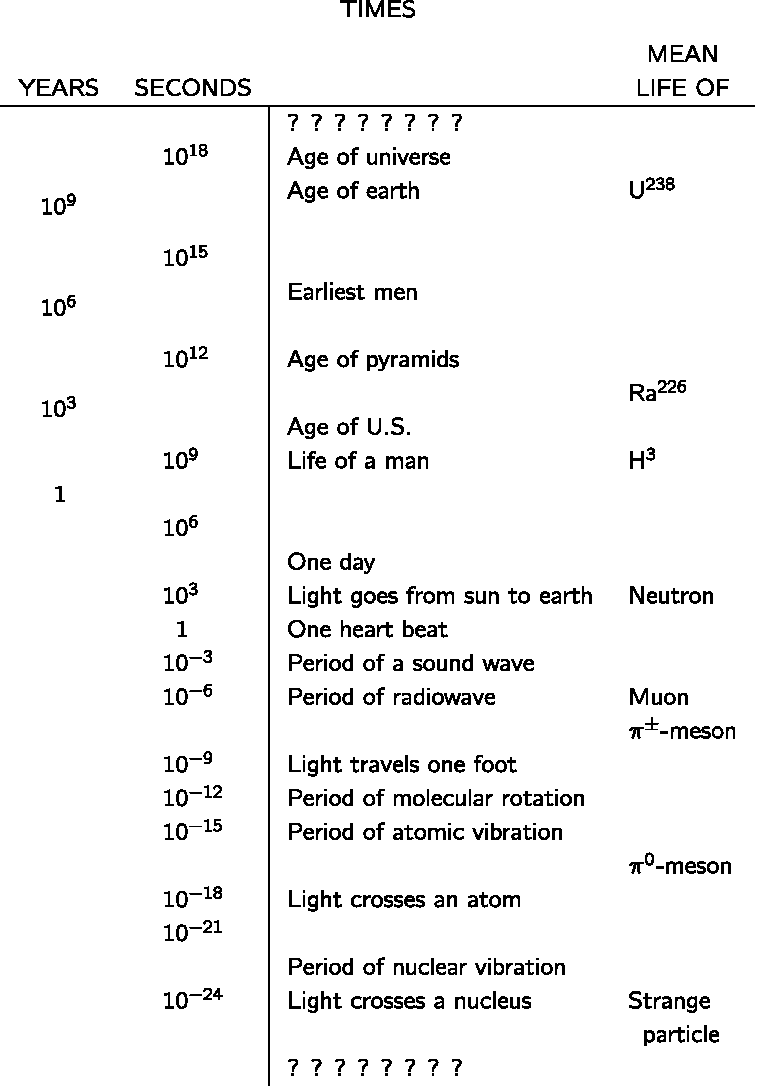
\includegraphics[width=0.8\linewidth]{fyz_fig074.pdf}
      \caption{Tabulka vzdáleností (\cite[s.~75]{Feynman01})}
      \label{fyz:fig074}
    \end{figure}
    
    Co zjišťujeme, jdeme-li k ještě menším vzdálenostem? Můžeme menší vzdálenosti měřit? Na tuto 
    otázku zatím není možné dát odpověď. Existuje hypotéza, podle níž je zatím nevyřešenou záhadu 
    jaderných sil možno odhalit jen jakousi modifikací naší představy o prostoru nebo o měření tak 
    malých vzdáleností.
    
    Zdálo by se rozumné použít za jednotku délky nějakou přirozenou délku - řekněme poloměr Země 
    nebo jeho zlomek. Metr byl původně navržen takovýmto způsobem a byl definován jako 
    \(\frac{\pi}{2}\cdot\num{e-7}\) násobek zemského poloměru. Takové určení délkové jednotky není 
    příliš výhodné ani příliš přesné. Dlouho byla obecně uznávána definice metru jako vzdálenosti 
    mezi dvěmi vrypy na tyči nacházející se ve speciální laboratoři ve Francii. Nedávno se však 
    zjistilo, že ani taková definice není dostatečně přesná, stálá a univerzální. Proto byla v r. 
    1983 přijata nová definice metru jako délka dráhy, kterou proběhne světlo ve vakuu za dobu 
    \(\frac{\num{1}}{\num{299792458}}\) sekundy.
    
    Měření vzdálenosti a času poskytují výsledky, které závisí na pozorovateli. Dva pozorovatelé, 
    kteří se vzájemně pohybují, nezměří stejné vzdálenosti a časy při měření toho, co se jeví jako 
    stejná věc. Vzdálenosti a časové intervaly mají různé velikosti v závislosti na vztažné 
    soustavě použité při měření. Tuto otázku budeme podrobněji studovat později.
    
    Zcela přesné měření vzdáleností a časů nedovoluje ani povaha přírody. Už dříve jsme řekli, že 
    chyba v měření polohy předmětu musí být přinejmenším
    \begin{equation}\label{FYZ:eq067}
      \Delta x = \frac{h}{\Delta p},
    \end{equation}
    kde \(h\) je malá veličina nazývaná \textbf{Planckova konstanta} a \(\Delta p\) je nepřesnost 
    našeho poznání hybnosti (hmotnosti násobené rychlostí) předmětu, jehož polohu měříme. Zmínili 
    jsme se i o tom, že neurčitost v měření polohy souvisí s vlnovou povahou částic.
    
    Relativnost prostoru a času znamená, že i měření času mají minimální chybu danou vztahem
    \begin{equation}\label{FYZ:eq068}
      \Delta t = \frac{h}{\Delta E},
    \end{equation}
    přičemž \(\Delta E\) je nepřesnost našeho poznání energie procesu, jehož časovou periodu 
    měříme. Chceme-li přesněji zjistit, kdy se něco uskutečnilo, musíme vědět méně o tom, co se 
    uskutečnilo, neboť budeme méně vědět o energii takového procesu. I Časová neurčitost souvisí s 
    vlnovou povahou hmoty.
    
} %tikzset
%---------------------------------------------------------------------------------------------------
\printbibliography[heading=subbibliography]
\addcontentsline{toc}{section}{Seznam literatury} 
%==== Kapitola: Teorie gravitace ===================================================================
% !TeX spellcheck = cs_CZ
{\tikzset{external/prefix={tikz/FYZI/}}
 \tikzset{external/figure name/.add={ch05_}{}}
%---------------------------------------------------------------------------------------------------
% file fey1ch07.tex
%---------------------------------------------------------------------------------------------------
\sisetup{quotient-mode = fraction}
%================ Kapitola: Teorie gravitace =======================================================
\chapter{Teorie gravitace}\label{fyz:chap_fey_gravity}
\minitoc
  \section{Pohyb planet}
    V této kapitole budeme hovořit o jednom z nejdalekosáhlejších zobecnění, které lidská mysl 
    uskutečnila. Zatímco obdivujeme lidskou mysl, měli bychom však postát s úctou před přírodou, 
    která tak dokonale splňuje skvělý a jednoduchý princip, jakým je gravitační zákon. Co to je, 
    ten gravitační zákon? Vyjadřuje skutečnost, že každý předmět ve vesmíru přitahuje kterýkoli 
    jiný předmět silou, která je pro libovolná dvě tělesa úměrná hmotnosti každého z nich a mění se 
    nepřímo úměrně čtverci vzdálenosti mezi nimi. Tento výrok lze matematicky vyjádřit vztahem
    \begin{equation}\label{FYZ:eq096}
      F = \kappa\frac{m_1m_2}{r^2}
    \end{equation}
    Uvedeme-li navíc skutečnost, že předmět reaguje na sílu zrychlením ve směru působení síly a 
    velikost zrychlení je nepřímo úměrná hmotnosti předmětu, poskytli jsme všechny potřebné 
    informace a dostatečně nadaný matematik je schopen odvodit všechny důsledky těchto dvou 
    principů.
    
    Zatím však nejsme dostatečně pokročilí, a proto budeme o důsledcích hovořit podrobněji a 
    nezůstaneme jen u samotných principů. Stručně připomeneme historii objevu gravitačního zákona a 
    pohovoříme o některých jeho důsledcích, jeho vlivu na historii, o záhadách, které se za tímto 
    zákonem skrývají a o tom, jak ho upřesnil Einstein. Budeme hovořit i o jeho vztahu k jiným 
    fyzikálním zákonům. Všechno však není možné stihnout v jedné kapitole, proto uvedeným problémům 
    věnujeme i následující kapitoly.
    
    Historie začíná u našich dávných předků, kteří pozorovali pohyb planet mezi hvězdami a nakonec 
    usoudili, že planety se pohybují kolem Slunce, což později znovu objevil Koperník. Trochu více 
    úsilí si vyžadovalo poznání toho, jak se planety kolem Slunce pohybují, jak jejich pohyb přesně 
    probíhá. Například smyčkovitý pohyb Marsu, znázorněný na obr. \ref{fyz:fig299}, byl obzvláště 
    matoucí.
    
    Na začátku patnáctého století se hodně diskutovalo o tom, jestli se planety opravdu pohybují 
    kolem Slunce nebo ne. Tycho Brahe (1546–1601) přišel se zcela novou myšlenkou. Spočívala v tom, 
    že tyto diskuse mohou vyřešit jen dostatečně přesná měření poloh planet na obloze. Ukáží-li 
    měření přesně, jak se planety pohybují, pak snad bude možné rozhodnout se pro jedno nebo druhé 
    stanovisko. Byla to úžasná myšlenka - že něco je lépe poznávat cestou pečlivých experimentů než 
    pokračováním v hlubokých filozofických úvahách. Při uskutečňování této myšlenky sledoval Tycho 
    Brahe ve své observatoři na ostrově Hven u Kodaně po dlouhá léta pohyby planet. Vyhotovil 
    rozsáhlé tabulky, které po jeho smrti studoval matematik \emph{Johannes Kepler} (1571–1630). 
    Kepler na základě těchto údajů objevil některé krásné, pozoruhodné a přitom jednoduché zákony 
    planetárního pohybu. Později ukázal Newton (1642–1727), že z jeho gravitačního zákona lze 
    Keplerovy empirické zákony odvodit i teoreticky.

    \begin{figure}[ht!]  %\ref{fyz:fig299}
      \centering
      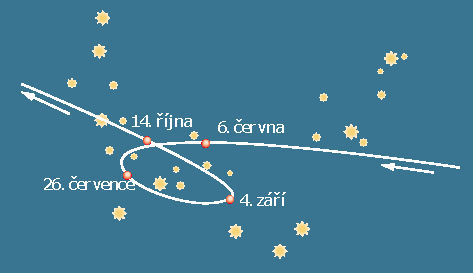
\includegraphics[width=0.8\linewidth]{fyz_fig299.pdf}
      \caption{Dráha planety Mars, po níž se pohybovala na pozadí souhvězdí Kozoroha během roku 
               1971. Na obrázku je znázorněna jeho poloha ve čtyřech různých dnech.Planety Marsi 
               Země se obě pohybují po oběžných drahách kolem Slunce; zde vidíme polohu Marsu 
               vzhledem k Zemi.Díky tomu pozorujeme na dráze Marsu zdánlivé smyčky. 
               (\cite[s.~366]{Halliday2001})}
      \label{fyz:fig299}
    \end{figure}
    
  \section{Keplerovy zákony}
    Kepler především zjistil, že každá planeta obíhá kolem Slunce po křivce nazývané 
    \textbf{elipsa}, přičemž Slunce se nachází v ohnisku elipsy. To je obsah \textbf{prvního 
    Keplerova} zákona. Elipsa není prostý ovál, ale představuje velmi svéráznou, přesné definovanou 
    křivku, kterou je možné získat tak, že tužkou napínáme nit upevněnou na dvou špendlíčkách 
    umístěných v ohniscích. Kdybychom se chtěli vyjádřit matematicky, museli bychom říci, že jde o 
    \emph{geometrické místo bodů, které mají stálý součet vzdáleností od dvou pevných bodů 
    (ohnisek)}. Nebo jestli se nám to líbí, je to kružnice, na kterou se díváme ze strany (obr. 
    \ref{fyz:fig062}).
    
    \begin{figure}[ht!]  %\ref{fyz:fig062}
      \centering
      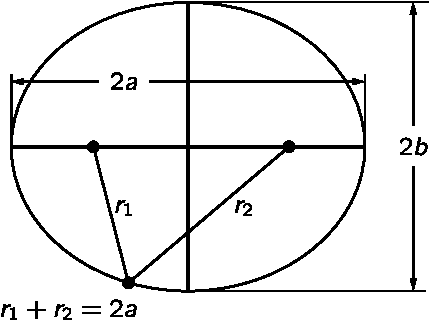
\includegraphics[width=0.5\linewidth]{fyz_fig062.pdf}
      \caption{Elipsa (\cite[s.~93]{Feynman01})}
      \label{fyz:fig062}
    \end{figure}
    \textbf{Druhým Keplerovým} poznatkem bylo zjištění, že planety neobíhají kolem Slunce stálou 
    rychlostí. Když jsou ke Slunci blíže, pohybují se rychleji, a když jsou od něho vzdálenější, 
    pohybují se pomaleji. Přesně můžeme tento pohyb popsat následujícím způsobem. Předpokládejme, 
    že pozorujeme planetu ve dvou po sobě jdoucích časových okamžicích, například časově vzdálených 
    o týden, a zakreslujeme průvodiče\footnote{Průvodič je úsečka spojující Slunce s kterýmkoliv 
    bodem na planetární dráze.} planety pro každou pozorovanou polohu. Přesně můžeme tento pohyb 
    popsat následujícím způsobem. Dráhový oblouk, který planeta prošla po týdnu a dva průvodiče 
    vymezují určitou plochu. Tato plocha představuje vyšrafovanou oblast na obr. \ref{fyz:fig063}. 
    Uskuteční-li se i druhé takové týdenní pozorování, a to tehdy, kdy je planeta dále od Slunce (a 
    má tedy menší rychlost), podobným způsobem vymezená plocha je přesné stejná, jako v 
    předcházejícím případě. \emph{Druhý Keplerův zákon tedy říká, že každá planeta obíhá kolem 
    Slunce takovou rychlostí, že plochy opsané průvodičem za stejnou dobu jsou stejné!}
    
    \begin{figure}[ht!]  %\ref{fyz:fig063}
      \centering
      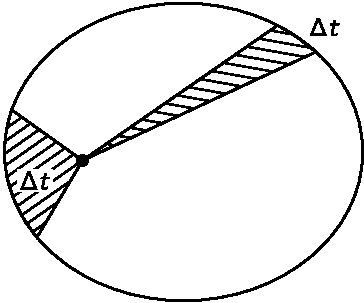
\includegraphics[width=0.5\linewidth]{fyz_fig063.pdf}
      \caption{Keplerův zákon ploch (\cite[s.~94]{Feynman01})}
      \label{fyz:fig063}
    \end{figure}
    \textbf{Třetí zákon} Kepler objevil mnohem později a patří do jiné kategorie než první dva, 
    neboť nehovoří jen o jedné planetě, ale dává do souvislosti jednotlivé planety. Tento zákon 
    porovnává periody (oběžné doby) a rozměry drah jednotlivých planet a říká, že periody jsou 
    úměrné \num{3/2} mocnině rozměrů drah. Periodou rozumíme dobu, který planeta potřebuje k oběhu 
    celé dráhy a rozměr se určuje délkou největšího průměru eliptické dráhy, známého jako 
    \emph{hlavní osa}. Kdyby se planety pohybovaly po kružnicích (a tato představa je dost blízko 
    skutečnosti), čas potřebný k opsání kružnice by byl úměrný \num{3/2} mocnině průměru (nebo 
    poloměru) kružnice. \textbf{Keplerovy zákony} tedy zní:
    
    \begin{enumerate}
      \item Každá planeta se pohybuje kolem Slunce po elipse, přičemž Slunce je v jednom z ohnisek.
      \item Průvodič spojující Slunce s planetou opisuje stejné plochy za stejné časové intervaly.
      \item Druhé mocniny period libovolných dvou planet jsou úměrné třetím mocninám velkých poloos 
            jejich drah \(T\approx a^\frac{3}{2}\).
    \end{enumerate}
    
  \section{Rozvoj Dynamiky}
    V době, kdy Kepler objevoval tyto zákony, Galileo se zajímal o zákony pohybu. Bylo třeba 
    objasnit, co nutí planety se pohybovat. (V té době jedna z „teorií“ planetárního pohybu 
    předpokládala, že příčinou pohybu planet jsou neviditelní andělé, kteří máváním svých křídel 
    tlačí planety dopředu v oběhu. Uvidíte, že dnes je již tato teorie pozměněná! Ukazuje se, že k 
    udržení planet musí neviditelní andělé působit na planety v jiném směru a nemají křídla. V 
    ostatním jsou však obě teorie podobné!) Galileo objevil pozoruhodnou vlastnost pohybu, jež byla 
    podstatnou pro pochopení těchto zákonů. Jde o \textbf{princip setrvačnosti} - jestliže se něco 
    pohybuje tak, že není s ničím ve styku a nic ho neruší, pak se bude pohybovat nepřetržitě podél 
    přímky a jeho rychlost bude \emph{konstantní}. (Proč pohyb neustane, to nevíme. Víme však, že 
    je to tak.)
    
    Newton upravil tuto myšlenku, když říkal, že jediným způsobem jak změnit pohyb tělesa je použít 
    \textbf{sílu}. Když se pohyb tělesa zrychluje, musela síla působit ve směru pohybu. Na druhé 
    straně, jestliže se změnil směr pohybu tělesa, síla působila ze strany. Newton tedy doplnil 
    tuto myšlenku o poznatek, že síla je potřebná ke změně velikosti rychlosti nebo směru pohybu 
    tělesa. Například, upevníme-li kámen na provaz a roztáčíme ho po kruhové dráze, potřebujeme 
    sílu, abychom ho na této dráze udrželi. Musíme tahat za provaz. Zákon ve skutečnosti říká, že 
    zrychlení vyvolávané silou je nepřímo úměrné hmotnosti tělesa, nebo, že síla je úměrná součinu 
    hmotnosti a zrychlení. Čím je těleso hmotnější, tím větší síla je potřebná k dosažení daného 
    zrychlení tělesa. (Hmotnost je možné měřit tak, že na konec stejného provazu upevňujeme různé 
    kameny a nutíme je pohybovat se po stejné kruhové dráze stejnou rychlostí. Tak zjistíme, že k 
    tomu je třeba větší nebo menší síly. Předměty vyžadující větší sílu, mají větší hmotnost.)
    
    Z těchto úvah vyplývá velkolepá myšlenka, že k udržení planet na jejich drahách nejsou potřebné 
    \emph{tangenciální síly} (andělé nemusí letět ve směru tečny), protože planeta i tak poletí v 
    daném směru. Kdyby planetu nic nerušilo, odletěla by \emph{přímočaře}. Skutečný pohyb se však 
    odchyluje od přímky, po níž by se těleso pohybovalo v nepřítomnosti sil, a tato odchylka je 
    \emph{kolmá} ke směru pohybu - tedy ne ve směru jeho pohybu. Jinými slovy: v důsledku principu 
    setrvačnosti není síla potřebná k udržení pohybu planet \emph{kolem} Slunce silou směřující 
    kolem Slunce, ale silou směřující ke Slunci. (Existuje-li tu síla směřující ke Slunci, může být 
    Slunce, samozřejmě, oním andělem!)
    
  \section{Newtonův gravitační zákon}
    Newton dokonaleji pochopil teorii pohybu a tak dospěl k přesvědčení, že \emph{právě Slunce} by 
    mohlo být místem nebo původcem sil, jež ovládají pohyb planet. Podařilo se mu dokázat (možná, 
    že to brzy dokážeme i my), že opisování stejných ploch za stejnou dobu znamená, že všechna 
    odchýlení od přímočarého pohybu jsou přesně \emph{radiální} - že zákon je přímým následkem 
    toho, že všechny síly \emph{směřují ke Slunci}
    
    Dále je možné analýzou třetího Keplerova zákona dokázat, že čím dále je planeta od Slunce, tím 
    jsou síly menší. Porovnáme-li dvě planety, různě vzdálené od Slunce, zjistíme, že síly jsou 
    nepřímo úměrné druhé mocnině odpovídajících vzdáleností. Kombinováním těchto dvou zákonů 
    usoudil Newton, že existuje síla, která je nepřímo úměrná druhé mocnině vzdálenosti a směřuje 
    po přímce, jež prochází dvěma na sebe působícími objekty.
    
    Newton, jenž měl značný smysl pro zobecnění, samozřejmě předpokládal, že tento vztah neplatí 
    jen pro Slunce přitahující planety. Tehdy se již například vědělo, že planeta Jupiter má 
    měsíce, které ji obíhají tak, jako zemský Měsíc obíhá Zemi a Newton si byl jistý, že každá 
    planeta přidržuje silou svůj měsíc ve své blízkosti. Newton již znal sílu, jež nás přidržuje na 
    Zemi, a tak předpokládal, že jde o \emph{univerzální} sílu - \emph{že vše je přitahováno vším}.
    
    Dále ho zajímalo, zda Země přitahuje stejnou silou lidi i Měsíc, tj. silou, jež je nepřímo 
    úměrná druhé mocnině vzdálenosti. Padá-li předmět na zemském povrchu \SI{5}{\m} za první 
    sekundu po vypuštění, o jakou vzdálenost spadne Měsíc za stejnou dobu? Je možné namítnout, že 
    Měsíc vůbec nepadá. Kdyby však na Měsíc nepůsobila síla, odletěl by po přímce, zatímco se 
    pohybuje po kružnici, takže skutečně padá z místa, na kterém by byl, kdyby na něj nepůsobily 
    síly. Protože známe poloměr jeho oběžné dráhy (asi \SI{380000}{\km}) a dobu oběhu Měsíce kolem 
    Země (přibližně \num{29} dní), můžeme vypočítat, jakou vzdálenost urazí Měsíc za \num{1} 
    sekundu a pak, o kolik za tuto dobu klesne\footnote{Tj. jak se kružnice oběžné dráhy Měsíce 
    odkloní od své tečny na úseku, který Měsíc urazí za 1 sekundu.}. Tato vzdálenost je přibližně 
    rovna \SI{1.4}{\mm} za sekundu. To zcela souhlasí se \emph{zákonem reciprokých čtverců}, neboť 
    zemský poloměr je roven \SI{6380}{\km} a padá-li v této vzdálenosti těleso o \SI{5}{\m} za 
    první sekundu, pak ve vzdálenosti \SI{380000}{\km}, tedy \num{60}-krát větší, by mělo spadnout 
    jen \num{1/3600} z \SI{5}{\m}, což je zhruba \SI{1.4}{\mm}. Podobnými výpočty Newton prověřoval 
    svou gravitační teorii. Výpočty provedl velmi pečlivě a zjistil tak velké odchylky, že 
    považoval teorii za protiřečící faktům a své výsledky nepublikoval. Po šesti letech byla 
    provedena nová měření zemských rozměrů, která ukázala, že astronomové používali nesprávnou 
    vzdálenost k Měsíci. Jakmile se o tom Newton doslechl, provedl své výpočty s opravenými údaji a 
    dospěl k překrásné shodě. Tj. jak se kružnice oběžné dráhy Měsíce odkloní od své tečny na 
    úseku, který Měsíc urazí za \num{1} sekundu.
    
    Myšlenka, že Měsíc „padá“, vyvolává rozpaky, neboť jak vidíme, Měsíc se k nám nepřibližuje. 
    Tato myšlenka je tak zajímavá, že si zasluhuje další vysvětlení: Měsíc padá v tom smyslu, že se 
    \emph{odklání od přímky, po níž by se pohyboval v nepřítomnosti sil}. Všimněme si příkladu ze 
    zemského povrchu. Předmět vypuštěný v blízkosti zemského povrchu padá \SI{5}{\m} za první 
    sekundu. I předmět vystřelený horizontálně spadne \SI{5}{\m}; ačkoli se pohybuje 
    \emph{horizontálně}, přece spadne za stejný čas o \SI{5}{\m}. Na obr. \ref{fyz:fig058} je 
    znázorněno zařízení na ověření této skutečnosti. Na horizontálním žlábku je míček, který se 
    bude pohybovat dopředu. Ve stejné výšce je míček, který bude padat vertikálně, přičemž 
    elektrický spínač je nastaven tak, že v okamžiku, kdy první míček opouští žlábek, uvolňuje se 
    druhý míček. Důkazem toho, že za stejnou dobu spadnou stejně hluboko, je jejich srážka ve 
    vzduchu.
    
    \begin{figure}[ht!]  %\ref{fyz:fig058}
      \centering
      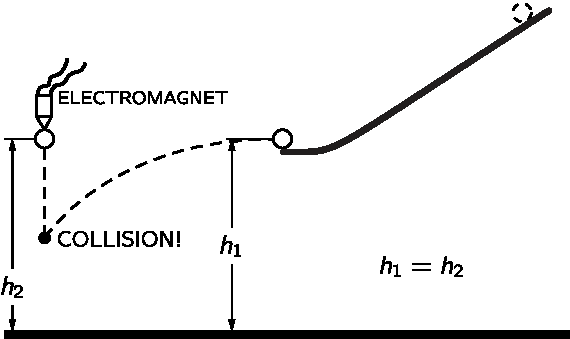
\includegraphics[width=0.7\linewidth]{fyz_fig058.pdf}
      \caption{Zařízení na demonstraci nezávislosti horizontálního a vertikálního pohybu 
               (\cite[s.~96]{Feynman01})}
      \label{fyz:fig058}
    \end{figure}
    Kulka vystřelená horizontálně, může za \num{1} sekundu proletět velkou vzdálenost - snad půl 
    kilometru - ale za ten čas spadne vždy o \SI{5}{\m}, byla-li vystřelená skutečně horizontálně. 
    Co se bude dít, budeme-li kulku vystřelovat rychleji a rychleji? Nesmíme zapomenout, že zemský 
    povrch je zakřivený. Vystřelíme-li kulku dostatečně rychle, může se stát, že ačkoli spadne o 
    \SI{5}{\m}, zůstane ve stejné výšce nad zemí, jako byla předtím. Jak je to možné? Ačkoli kulka 
    padá, Země se zakřivuje a tak se stává, že kulka padá \uv{kolem} Země. Je však třeba odpovědět 
    na otázku, jak daleko se musí dostat kulka za jednu sekundu, aby země byla \SI{5}{\m} pod 
    horizontem. Na obr. \ref{fyz:fig059} je znázorněna Země s jejím \SI{6380}{\km} dlouhým 
    poloměrem a tečna - přímka, po níž by se kulka pohybovala v nepřítomnosti sil. Použijeme-li 
    jednu z nádherných geometrických pouček, která říká, že naše tečna je geometrický průměr dvou 
    částí průměru vyťatých stejně dlouhou tětivou, zjistíme, že horizontální vzdálenost, kterou 
    kulka urazí, je geometrický průměr z \SI{5}{\m} pádu a \SI{12760}{\km} zemského průměru. Druhá 
    odmocnina z (\(\num{0.005}\times\num{12760}\)) vychází přibližně \SI{7.9}{\km}. Pohybuje-li se 
    tedy kulka rychlostí \SI{7.9}{\km} za sekundu, bude padat k Zemi každou sekundu o \SI{5}{\m}, 
    ale nikdy se k Zemi nepřiblíží, neboť Země je zakřivená. Tak to bylo i s Gagarinem, který 
    obíhal Zemi rychlostí přibližně \SI{8}{\km/\sec} po \SI{40000}{\km} dlouhé oběžné dráze. (Ve 
    skutečnosti trochu více, neboť letěl výše.)

    \begin{figure}[ht!]  %\ref{fyz:fig089}
      \centering
      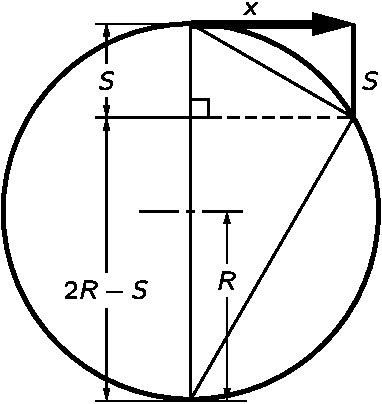
\includegraphics[width=0.5\linewidth]{fyz_fig059.pdf}
      \caption{Dostředivé zrychlení při kruhové dráze. Z podobnosti trojúhelníku: \(\frac{x}{s} = 
               \frac{(2R - s)}{x} \approx \frac{2R}{x}\) kde \(R\) je poloměr Země             
               (\SI{6380}{\km}), \(x\) je vzdálenost „prošlá horizontálně a za jednu sekundu a 
               \(s\) je vzdálenost \uv{padání} za jednu sekundu (přibližně \SI{5}{\m}) 
               \cite[s.~97]{Feynman01}}
       \label{fyz:fig059}
    \end{figure}
    
    Každý objev nového zákona je užitečný jen tehdy, když je z něho možné získat více, než bylo do 
    něho vloženo. Newton použil druhý a třetí Keplerův zákon k odvození svého gravitačního zákona. 
    Co předpověděl? Nejdříve to byla jeho analýza pohybu Měsíce, neboť dávala do souvislosti padání 
    předmětů na Zemi s \uv{padáním} Měsíce. Druhou předpovědí byla odpověď na otázku, zda jsou 
    dráhy planet elipsy. Později uvidíme, jak je možno přesně vypočítat tento pohyb a dokázat, že 
    planety se skutečně pohybují po elipsách. Takže žádná jiná fakta k důkazu prvního Keplerova 
    zákona nepotřebujeme. Tak Newton uskutečnil svou první velkou předpověď.

    Gravitační zákon vysvětluje mnoho dříve nepochopených jevů, například do té doby záhadný jev 
    \textbf{slapových pohybů} - \emph{přílivu a odlivu} - způsobovaných měsíční přitažlivostí. Lidé 
    se i předtím domnívali, že Měsíc přitahuje vodu pod sebou a způsobuje příliv, ale nebyli tak 
    bystří jako Newton, a proto si mysleli, že by měl být jen jeden příliv za den. Předpokládalo 
    se, že Měsíc přitahuje vodu a vyvolává tak příliv a odliv a protože se Země otáčí, měl by v 
    každém místě nastat příliv a odliv za \num{24} hodin. Skutečnost je však taková, že příliv a 
    odliv nastávají každých \num{12} hodin. Podle jiných představ měl zase příliv nastat na opačné 
    straně Země, neboť Měsíc odtahuje Zemi od vody! Obě dvě tyto teorie jsou nesprávné. Proces 
    probíhá následujícím způsobem: měsíční přitažlivost Země i vody je ve středu Země, v průměru 
    vyvážená. Avšak voda, která je blíže k Měsíci, je přitahována více než je průměrná 
    přitažlivost, zatímco voda na vzdálenější straně je přitahována méně než je průměrná 
    přitažlivost. Navíc, voda může téct, zatímco pevná Země ne. To, co skutečně pozorujeme, je pak 
    kombinace těchto dvou úkazů.

    \begin{figure}[ht!]  %\ref{fyz:fig060}
      \centering
      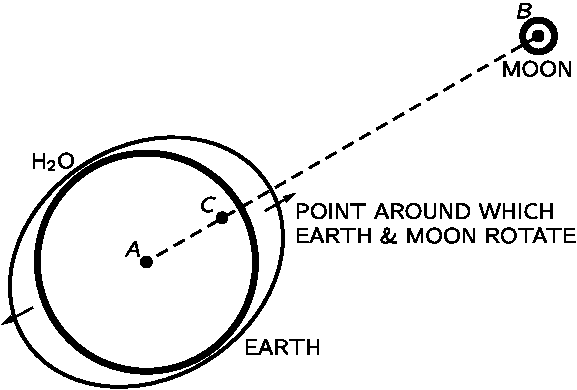
\includegraphics[width=0.7\linewidth]{fyz_fig060.pdf}
      \caption{Slapové pohyby v soustavě Země - Měsíc (\cite[s.~97]{Feynman01})}
      \label{fyz:fig060}
    \end{figure}
    Co chápeme pod slovem „vyvážený“? Co je vyvážené? Přitahuje-li Měsíc celou Zemi, proč ta 
    nespadne „nahoru“ na Měsíc? Ze stejné příčiny, ze které Měsíc nespadne na Zemi. Země obíhá 
    kolem bodu, jenž leží v jejím nitru, ale není v jejím středu. Měsíc neobíhá jen kolem Země, ale 
    Země i Měsíc obíhají kolem centrální polohy a obě tělesa padají na toto společné centrum, jak 
    je to znázorněno na obr. \ref{fyz:fig060}. Tento pohyb kolem společného centra je tím, co 
    vyvažuje pád každého z těchto těles. Ani Země se tedy nepohybuje po přímce, ale po kružnici. 
    Voda na vzdálenější straně je „nevyvážená“, neboť vjejím místě je měsíční přitažlivost slabší 
    než ve středu Země, kde vyvažuje „odstředivou“ sílu. Výsledkem této nevyváženosti je, že voda 
    se zvedá směrem od středu Země. Na bližší straně je měsíční přitažlivost silnější a 
    nevyváženost má opačný směr v prostoru, ale opět směřuje pryč od středu Země. Výsledkem je 
    existence dvou přílivových vzdutí.
    
  \section{Všeobecná gravitace}
    Co ještě můžeme pochopit, známe-li gravitaci? Každý ví, že Země je kulatá. Proč je Země kulatá? 
    To je jednoduché; následkem gravitace. Země je kulatá proto, že všechno se navzájem přitahuje a 
    tak se to, z čeho Země vznikla, přitahovalo, dokud to bylo možné! Chceme-li být přesnější, Země 
    není přesná koule, neboť rotuje a tato rotace vede k odstředivému působení, jež zmenšuje 
    gravitační působení v blízkosti rovníku. Země by tedy měla být elipsoidem, jehož přesný tvar 
    dokonce umíme určit. Z gravitačního zákona tedy můžeme usoudit, že Slunce, Měsíc i Země by měly 
    mít (přibližně) kulový tvar.
    
    Co ještě můžeme určit z gravitačního zákona? Podíváme-li se na měsíce Jupitera, pochopíme vše o 
    způsobu jejich pohybu kolem této planety. Mimochodem, jednou byl problém právě s měsíci 
    Jupitera a nebude od věci něco si o tom říci. Tyto měsíce velmi podrobně studoval Roemer a 
    všiml si, že někdy předbíhají \uv{letový řáď} a někdy se zase opožďují. (Jejich \uv{letový řáď} 
    je možné sestavit po velmi dlouhém pozorování zjištěním průměrné doby obletu.) Měsíce 
    předbíhaly řád, když byl Jupiter obzvláště blízko k Zemi a opožďovaly se, když byl Jupiter 
    vzdálený od Země. Je to velmi těžké vysvětlit podle gravitačního zákona - dokonce by to mohlo 
    pohřbít tuto nádhernou teorii, kdyby neexistovalo jiné vysvětlení. Kdyby totiž zákon 
    nevyhovoval třeba jen v jednom případě, v němž by měl platit, byl by nesprávný. Tento rozpor se 
    však dal vysvětlit velmi jednoduše a krásně: K tomu, abychom pozorovali měsíce Jupitera, je 
    potřebný určitý čas, za který světlo urazí vzdálenost od Jupitera k Zemi. Je-li Jupiter 
    \emph{blíže} k Zemi, čas je \emph{kratší} a je-li Jupiter \emph{dále}, čas je \emph{delší}. 
    Proto se měsíce zdánlivě jednou předbíhají a jindy opožďují za letovým řádem, podle toho, zda 
    jsou blíže nebo dále od Země. Tento úkaz, který svědčí o tom, že světlo se nešíří okamžitě, 
    poskytl první odhad rychlosti šíření světla. Bylo to roku 1656.
    
    Při\-ta\-hují-li se vzájemně všechny planety, pak síla, která ovládá například Jupiter na jeho 
    cestě kolem Slunce, nepochází jen od Slunce; pochází například i od Saturnu. Ačkoli tato síla 
    není velká, neboť Slunce má mnohem větší hmotnost než Saturn, přece to je jen určitá síla a 
    dráha Jupitera by neměla být - a ani není - dokonalou elipsou; je trochu vychýlená a 
    \uv{kolísá} kolem skutečně eliptické dráhy. Takový pohyb je trochu komplikovanější. Byly 
    uskutečněny pokusy o analýzu pohybu Jupitera, Saturnu a Uranu na základě gravitačního zákona. 
    Započítaly se vlivy jednotlivých planet, aby se zjistilo, jestli tento zákon vysvětluje drobné 
    odchylky a nepravidelností v jejich pohybu. A hle - v případě Jupitera a Saturnu bylo vše v 
    pořádku, ale Uran se choval velmi podivně. Nepostupoval po přesné elipse, jenže to se dalo 
    pochopit jako následek přitažlivosti Jupitera a Saturnu. Když se však započítaly i tyto 
    přitažlivosti, Uran se \emph{stále} pohyboval nepravidelně a hrozilo, že gravitační zákon není 
    správný. Adams v Anglii a Leverrier ve Francii přišli nezávisle na sobě na jinou možnost: možná 
    že existuje jiná planeta, tmavá a neviditelná, kterou lidé zatím neobjevili. Tato planeta N by 
    měla přitahovat Uran. Vypočítali, kde by se měla taková planeta nacházet, aby způsobovala 
    pozorované odchylky. Pak zaslali zprávy příslušným observatořím, aby namířily dalekohledy na 
    vypočtené místo, kde je možné vidět novou planetu. Aby vás brali vážně, to často závisí na tom, 
    s kým pracujete. Leverriera brali vážně, podívali se na určené místo a planetu N skutečně 
    našli! Za krátkou dobu i další observatoř našla tuto planetu.

    \begin{figure}[ht!]  %\ref{fyz:fig089}
      \centering
      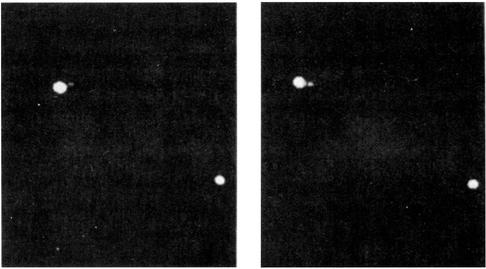
\includegraphics[width=0.8\linewidth]{fyz_fig089.jpg}
      \caption{Systém dvojhvězdy (\cite[s.~99]{Feynman01})}
      \label{fyz:fig089}
    \end{figure}
    
    Tento objev potvrzuje, že Newtonovy zákony jsou zcela správné v sluneční soustavě, ale zůstává 
    otázka, zda jsou správné i při větších vzdálenostech, než jsou relativně malé vzdáleností 
    nejbližších planet. Nejprve si můžeme položit otázku: Přitahují se hvězdy vzájemně také tak 
    jako planety? Přesvědčivý důkaz takové přitažlivostí máme v případě dvojhvězd Na obr. 
    \ref{fyz:fig089} je vidět dvojhvězdu - dvě hvězdy, jež jsou velmi blízko u sebe (je tam i třetí 
    hvězda, a proto se můžeme přesvědčit, zda fotografie nebyla otočená). Obrázek nám ukazuje i 
    konfiguraci hvězd po několika letech. Je vidět, že vzhledem k \uv{pevné} hvězdě se osa páru 
    pootočila, tj. hvězdy obíhají jedna kolem druhé. Obíhají podle Newtonových zákonů? Pečlivá 
    měření relativních poloh jedné takové dvojhvězdy jsou zakreslena na obr. \ref{fyz:fig090}. 
    Měření, která se uskutečnila mezi roky \num{1862} a \num{1904} (do dnešních dnů se musel 
    uskutečnit už i další oběh), dávají krásnou elipsu. Vše souhlasí s Newtonovými zákony, až na to 
    že hvězda Sírius A \emph{není v ohnisku}.  

    \begin{figure}[ht!]  %\ref{fyz:fig090}
      \centering
      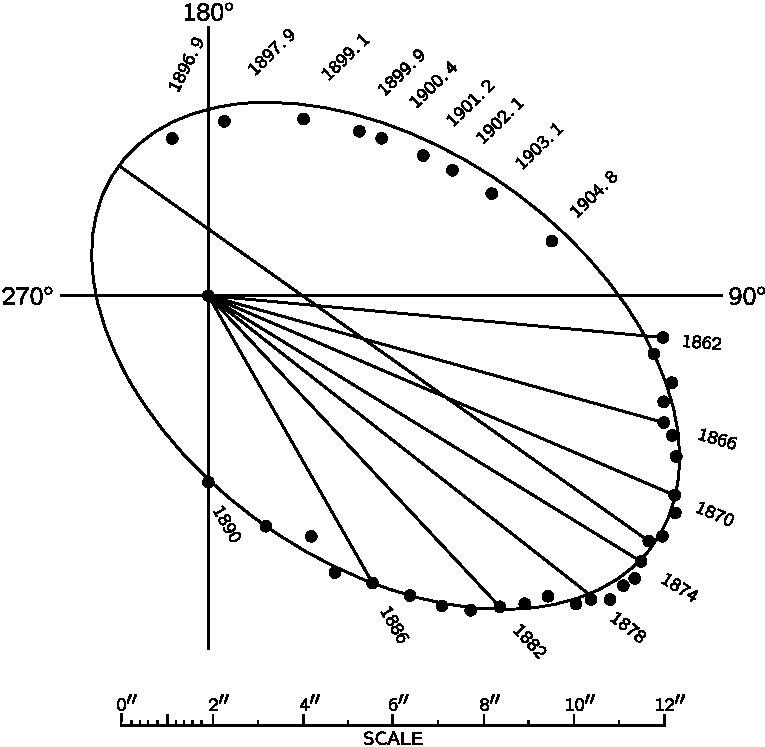
\includegraphics[width=0.8\linewidth]{fyz_fig090.pdf}
      \caption{Dráha Síra B vzhledem k Síriu A (\cite[s.~99]{Feynman01})}
      \label{fyz:fig090}
    \end{figure}
    
    Proč dochází k něčemu takovému? Protože rovina elipsy není v \uv{rovině oblohy}. Na rovinu 
    dráhy se nedíváme pod pravým úhlem a když hledíme na nakloněnou elipsu, zůstane stále elipsou, 
    ale ohnisko nezůstane na původním místě. Tak můžeme relativní pohyb dvojhvězd analyzovat v 
    souladu s požadavky gravitačního zákona. 
    
    Pravdivost gravitačního zákona i na větších vzdálenostech potvrzuje obr. \ref{fyz:fig092}. Jen 
    člověk bez představivosti na něm nevidí působení gravitace. Tento obrázek znázorňuje jednu z 
    nejkrásnějších věcí na obloze - kulovou hvězdokupu. Každá tečka je hvězda. Ačkoli hvězdy 
    vypadají, jako by byly pevně natlačeny k centru, jde pouze o nedokonalost našich přístrojů. Ve 
    skutečnosti jsou i vzdálenosti mezi středovými hvězdami velmi velké a jen velmi zřídka tu 
    dochází ke srážkám. Nejvíce hvězd je ve středu a se vzdalováním se od středu počet hvězd klesá. 
    Je zřejmé, že mezi těmito hvězdami existuje přitažlivost. 
    
    \begin{figure}[ht!]  %\ref{fyz:fig092}
      \centering
      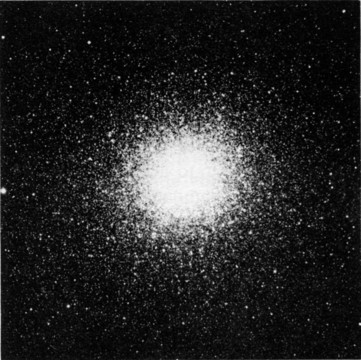
\includegraphics[width=0.8\linewidth]{fyz_fig092.jpg}
      \caption{Kulová hvězdokupa (\cite[s.~100]{Feynman01})}
      \label{fyz:fig092}
    \end{figure}
    Je jasné, že na těchto ohromných vzdálenostech, \num{100000}-krát větších než je sluneční 
    soustava, existuje gravitační síla. Pojďme však dále a podívejme se na \emph{celou galaxii} 
    znázorněnou na obr. \ref{fyz:fig093}. Tvar této galaxie svědčí o zjevné snaze její hmoty 
    aglomerovat. Samozřejmě nemůžeme dokázat, že tu jde přesně nepřímou úměrnost druhé mocnině 
    vzdálenosti, ale jen to, že i na těchto ohromných vzdálenostech je to přitažlivost, která drží 
    věci pohromadě. Je možné namítnout, že je to sice všechno pěkné, ale proč nemá galaxie kulový 
    tvar? Protože rotuje a má moment hybnosti, jehož se nemůže vzdát při smrštění; musí tedy být 
    smrštěna převážně v rovině. (Mimochodem, hledáme-li zajímavý problém, tak zatím nevíme, jak se 
    tvoří spirální ramena galaxie a co určuje tvar galaxií.) Je ale jasné, že tvar galaxie je určen 
    gravitací, i když složitost jeho struktury nám zatím brání úplně ho analyzovat. Rozměry galaxií 
    jsou asi od \num{50000} do \num{100000} světelných let. Jak velké jsou to vzdálenosti si 
    uvědomíme až tehdy, když uvážíme, že vzdálenost Země od Slunce je  \(8\tfrac{1}{3}\) světelných 
    minut. 
    
    \begin{figure}[ht!]  %\ref{fyz:fig093}
      \centering
      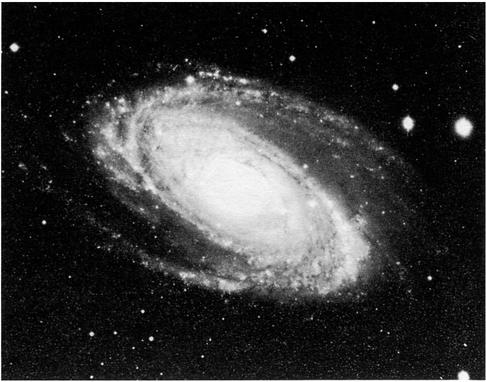
\includegraphics[width=0.8\linewidth]{fyz_fig093.jpg}
      \caption{Galaxie (\cite[s.~99]{Feynman01})}
      \label{fyz:fig093}
    \end{figure}
    
    Zdá se, že přitažlivost existuje i ve větších vzdálenostech. Obr. \ref{fyz:fig094} znázorňuje 
    shluk mnoha \uv{drobných} útvarů. Je to kupa \emph{galaxií}, podobná hvězdokupě. Galaxie se 
    tedy v takových vzdálenostech přitahují, a proto aglomerují do větších celků.

    \begin{figure}[ht!]  %\ref{fyz:fig094}
      \centering
      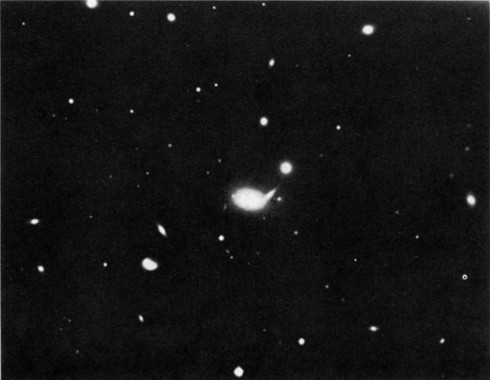
\includegraphics[width=0.8\linewidth]{fyz_fig094.jpg}
      \caption{Kupa galaxií (\cite[s.~100]{Feynman01})}
      \label{fyz:fig094}
    \end{figure}
    
    Gravitace snad existuje i ve vzdálenostech \emph{desítek miliónů} světelných let. Podle našich 
    dosavadních znalostí je gravitační síla všude nepřímo úměrná mocnině vzdálenosti. 

    \begin{figure}[ht!]  %\ref{fyz:fig095}
      \centering
      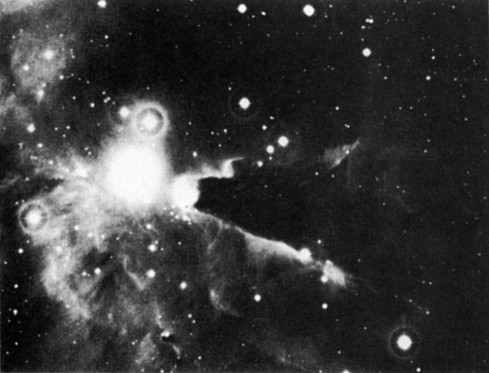
\includegraphics[width=0.8\linewidth]{fyz_fig095.jpg}
      \caption{Mezihvězdný prachový oblak (\cite[s.~101]{Feynman01})}
      \label{fyz:fig095}
    \end{figure}
    
    Gravitační zákon nám dovoluje pochopit nejen povahu mlhovin, ale poskytuje nám i určité 
    představy o původu hvězd. Máme-li velký oblak prachu a plynu podobný tomu, jenž je je znázorněn 
    na obr. \ref{fyz:fig095}, vzájemná přitažlivost prachových částic může vyvolat jejich seskupení 
    do malých hrudek. Na obrázku slabě viditelné \uv{malé} černé skvrnky mohou být začátkem 
    akumulace prachu a plynů, které díky své přitažlivosti začínají tvořit hvězdy. Je diskutabilní, 
    zda jsme vůbec někdy viděli zrod hvězdy. Na obr. \ref{fyz:fig096} je možná důkaz toho, že ano. 
    Na levé straně je obrázek oblasti plynu s několika hvězdami. Tento snímek pochází z roku 
    \num{1947}. Na pravé straně je obrázek o sem let mladší. Na něm jsou vidět dvě nové jasné 
    skvrny. Akumuloval se plyn a gravitace vyvolal jeho soustředění do dostatečně velké koule,takže 
    začala hvězdná jaderná reakce a přeměnila ho na hvězdu? Možná ano, možná ne. Je však 
    nepravděpodobné, že za pouhých sedm let bychom měli štěstí vidět přeměnu hvězdy do viditelné 
    podoby a ještě méně pravděpodobné je vidět takové přeměny hned dvě!

    \begin{figure}[ht!]  %\ref{fyz:fig096}
      \centering
      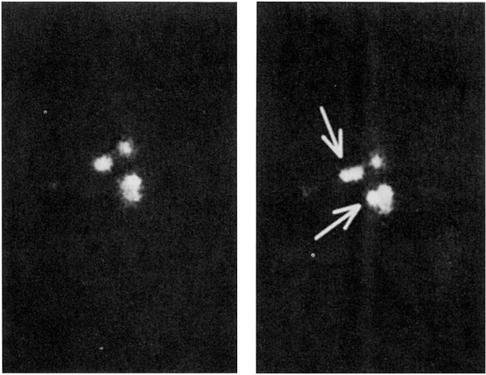
\includegraphics[width=0.8\linewidth]{fyz_fig096.jpg}
      \caption{Vznik nových hvězd? (\cite[s.~101]{Feynman01})}
      \label{fyz:fig096}
    \end{figure}
    
  \section{Cavendishův experiment}
    Gravitace tedy působí na obrovských vzdálenostech. Existuje-li však síla mezi 
    \emph{libovolnými} dvěma předměty, pak musí existovat možnost změřit tuto sílu působící mezi 
    předměty v našem okolí. Nemohli bychom namísto pozorování pohybu hvězd vzít olověnou a 
    mramorovou kuličku a pozorovat jak se bude pohybovat mramorová kulička k olověné? Obtížnost tak 
    jednoduchého experimentu spočívá v tom, že tato síla je sama velmi malá, jemná. Pokus je třeba 
    provádět s mimořádnou pečlivostí, což znamená vyčerpat vzduch z aparatury, vyloučit přítomnost 
    elektrických nábojů apod., a až potom je možné tu sílu měřit. Poprvé provedl takovéto měření 
    Cavendish na zařízení, které je schématicky znázorněno na obr. 7.13. Tímto pokusem se poprvé 
    dokazovala přímá síla mezi dvěma velkými pevnými olověnými koulemi a dvěma menšími olověnými 
    koulemi umístěnými na koncích vahadla upevněného na velmi jemném, tzv. torzním, vlákně. Měřením 
    zkroucení vlákna je možné měřit velikost síly a přesvědčit se, že je nepřímo úměrná druhé 
    mocnině vzdálenosti. Takto je možné přesně určit koeficient \(\kappa\) ve vztahu
    \begin{equation}\label{FYZ:eq094}
      F = \kappa\frac{m_1m_2}{r^2}.
    \end{equation}
    
    \begin{figure}[ht!]  %\ref{fyz:fig091}
      \centering
      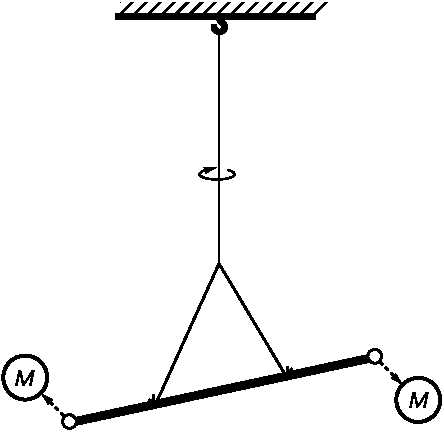
\includegraphics[width=0.5\linewidth]{fyz_fig091.pdf}
      \caption{Zjednodušené schéma zařízení, pomocí něhož Cavendish ověřoval gravitační zákon v 
               případě malých objektů a měřil gravitační konstantu \(\kappa\)
               (\cite[s.~102]{Feynman01})}
      \label{fyz:fig091}
    \end{figure}
    Všechny hmotnosti a vzdálenosti známe. Možná namítnete, že jsme je znali i v případě Země. Ano, 
    znali jsme vše, až na \emph{hmotnost Země}. Určením \(\kappa\) z tohoto experimentu a poznáním 
    zemské přitažlivosti můžeme nepřímo určit hmotnost Země! Tento experiment byl nazván „vážením 
    Země“. Cavendish tvrdil, že vážil Zemi, ale to, co skutečně měřil, byl koeficient \(\kappa\) 
    gravitačního zákona. To je jediný způsob jak je možné určit hmotnost Země.
    
    Koeficient \(\kappa\) je roven 
    \begin{equation}\label{FYZ:eq095}
      \kappa = \SI{6.670e-11}{\N\square\meter\per\square\kg}.
    \end{equation}
    
    Je těžké přecenit důležitost vlivu velkého úspěchu gravitační teorie na historii vědy. Stačí 
    porovnat tehdejší zmatek, neúplné poznatky, nedůvěru, nekonečné debaty a paradoxy s jasností a 
    jednoduchostí tohoto zákona; s tím, že všechny měsíce, planety a hvězdy jsou \emph{ovládány tak 
    jednoduchým pravidlem}, kterému člověk \emph{rozumí} a umí z něho odvodit, jak se planety musí 
    pohybovat! V tom je třeba vidět příčinu úspěchu věd v následujících letech. Tento poznatek dal 
    lidem naději, že i jiné jevy mohou mít tak krásně jednoduché zákony.
    
  \section{Co je to gravitace?}
    Je to však skutečně tak jednoduchý zákon? Co je možné říci o jeho příčině? Dosud jsme jen 
    popisovali, \emph{jak} se Země pohybuje kolem Slunce, ale nehovořili jsme o tom, co 
    \emph{vyvolává tento pohyb}. Newton se vědomě nezabýval tímto problémem; nevymýšlel si 
    hypotézy. Uspokojil se s poznáním toho, co se odehrává, bez poznání mechanizmu. \emph{Dosud 
    však nikdo takový mechanizmus neobjevil}. Fyzikální zákony se vyznačují právě takovýmto 
    abstraktním charakterem. Zákon zachování energie je tvrzení týkající se veličin, jež je třeba 
    vypočítat a sčítat, a není v něm zmínky o mechanizmu. Podobně je to i s velkými zákony 
    mechaniky, které jsou kvantitativními matematickými zákony, jejichž vnitřní mechanizmus 
    neznáme. Proč k popisu přírody můžeme používat matematiku, aniž bychom věděli, jaký mechanizmus 
    se za tím skrývá? To neví nikdo. Musíme to dělat i nadále, neboť tak se můžeme více dozvědět.
    
    Bylo navrženo mnoho mechanizmů gravitace. Bude zajímavé si všimnout jednoho z nich, k němuž se 
    lidé čas od času vracejí. Zpočátku každý, kdo takovýto mechanizmus „objeví“, je vzrušený a 
    šťastný, ale brzy zjistí, že mechanizmus není správný. Poprvé byl objeven kolem roku 
    \num{1750}. Představte si, že v prostoru je velké množství částic, jež se pohybují velkou 
    rychlostí ve všech směrech a při průchodu hmotou jsou jen velmi málo absorbovány. Když jsou 
    absorbovány Zemí, ode vzdávají jí hybnost. Protože je těch, které letí jedním směrem, stejně 
    mnoho jako těch, které letí opačným směrem, hybnosti jsou vyvážené. Když se však přiblíží 
    Slunce, jsou částice přicházející na Zemi skrz Slunce částečně absorbovány a ve směru od Slunce 
    přichází méně částic než z opačné strany. Země proto získá hybnost směřující ke Slunci a nedá 
    mnoho práce zjistit, že síla bude nepřímo úměrná druhé mocnině vzdálenosti - tak se totiž se 
    vzdáleností mění prostorový úhel, pod nímž vidíme Slunce. Co je na tomto mechanizmu špatně? 
    Zahrnuje některé nové důsledky, které \emph{nejsou správné}. Taková myšlenka totiž vede k 
    následujícímu problému: Země by při svém pohybu kolem Slunce narážela na více částic zepředu 
    než zezadu. (Když běžíte v dešti, je déšť do tváře silnější než déšť do týla!). Země by proto 
    měla dostávat více hybnosti zepředu a měla by proto pociťovat \emph{odpor} a zpomalovat se. Je 
    možné spočítat, jaký čas by potřebovala Země k zastavení v důsledku takovéhoto odporu; ukazuje 
    se, že Země by se už měla pomalu zastavit, takže tento mechanizmus selhává. Zatím se nenašel 
    žádný mechanizmus, jenž by vysvětloval „gravitaci“ bez předpovězení jiných jevů, které však 
    \emph{neexistují}.
    
    Všimněme si ještě možného vztahu gravitace k jiným silám. Zatím neexistuje vysvětlení gravitace 
    pomocí jiných sil. Gravitace není projevem elektřiny nebo něčeho podobného, takže vysvětlení 
    nemáme. Gravitace je však jiným silám velmi podobná a je zajímavé blíže si všimnout této 
    podobnosti. Například elektrická síla mezi dvěma nabitými předměty připomíná gravitační zákon: 
    je rovna záporné konstantní veličině násobené součinem nábojů a mění se nepřímo úměrně s druhou 
    mocninou jejich vzdálenosti. Působí na opačnou stranu - způsobuje odpuzování. Není přece jen 
    velmi pozoruhodné, že tyto dva zákony obsahují stejnou funkci vzdálenosti? Možná, že mezi 
    gravitací a elektřinou je mnohem větší souvislost než si myslíme. Bylo uskutečněno mnoho pokusů 
    o sjednocení elektřiny a gravitace, takzvaná jednotná teorie pole je pouze velmi elegantním 
    pokusem zkombinovat elektřinu a gravitaci. Při porovnávání gravitace a elektřiny je 
    nejzajímavější \emph{relativní velikost} sil. Každá teorie, která je obsahuje obě dvě, musí 
    objasnit i velikost gravitace.
    
    Určíme-li v nějakých přirozených jednotkách odpuzování dvou elektronů (univerzální náboj 
    přírody) způsobené elektrickými silami a přitažlivost těchto elektronů způsobenou jejich 
    hmotnostmi, můžeme určit poměr elektrického odpuzování a gravitačního přitahování. Tento poměr 
    nezávisí na vzdálenosti a je základní konstantou přírody. Je znázorněn na obr. 
    \ref{fyz:fig097}. Poměr gravitační přitažlivosti a elektrického odpuzování dvou elektronů je 
    \num{1 /4.17e42}! Kde se vzalo tak velké číslo? Určitě není výsledkem náhody - vždyť nejde o 
    poměr velikosti Země a blechy. Uvažovali jsme dvě přirozené vlastnosti stejné věci - elektronu. 
    Toto fantastické číslo je přirozenou konstantou; skrývá v sobě jakési tajemství přírody. Jak se 
    mohlo tak ohromné číslo objevit? Jsou lidé, kteří tvrdí, že jednou objevíme „univerzální 
    rovnici“ a jedním z jejích kořenů bude právě toto číslo. Je však velmi těžké najít rovnici, 
    jejímž přirozeným kořenem by bylo tak fantastické číslo. Uvažovalo se i o jiných možnostech a 
    jedna z nich dává uvedené číslo do souvislosti s věkem vesmíru. Prostě musíme někde najít jiné 
    tak velké číslo. Ale máme na mysli věk vesmíru vyjádřený v rokách? Ne, protože roky nejsou 
    „přirozené“; ty vymyslel člověk. Jako příklad něčeho přirozeného uvažujme čas, za který světlo 
    projde protonem, tj. \SI{e-24}{\s}. Porovnáme-li tento čas s \textbf{věkem vesmíru}, který je 
    \num{2e10} let, dostaneme \num{e-42}. Protože má toto číslo přibližně stejný počet nul, byla 
    gravitační konstantě přisouzena souvislost s věkem vesmíru. Je-li to pravda, pak se gravitační 
    konstanta musí měnit s časem, neboť jak vesmír stárne, postupně roste poměr mezi jeho věkem a 
    časem, který potřebuje světlo k průchodu protonem. Je možné, že gravitační konstanta se 
    \emph{mění} s časem? Je jasné, že změny by byly tak malé, že přesvědčit se o nich by bylo velmi 
    obtížné.
    
    \begin{figure}[ht!]  %\ref{fyz:fig097}
      \centering
      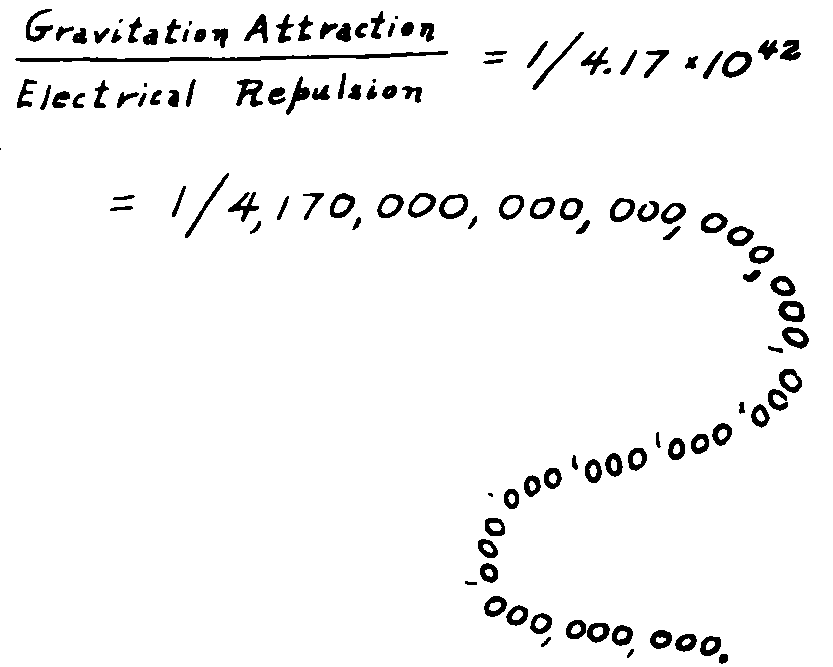
\includegraphics[width=0.7\linewidth]{fyz_fig097.pdf}
      \caption{Relativní síla elektrické a gravitační interakce mezi dvěma elektrony
               (\cite[s.~104]{Feynman01})}
      \label{fyz:fig097}
    \end{figure}
    Jedním ze způsobů ověření je zjistit, jaký vliv by měla změna gravitační konstanty v průběhu 
    posledních \num{e9} let, což představuje přibližně období od začátku života na Zemi až dodnes 
    nebo jednu desetinu stáří vesmíru. Za toto období by měla gravitační konstanta vzrůst asi o 
    10\%. Kdybychom uvažovali strukturu Slunce - rovnováhu mezi jeho hmotností a rychlostí, kterou 
    je v něm generována zářivá energie - dospěli bychom k závěru, že při gravitaci o 10\% větší by 
    mělo být Slunce mnohem více než o 10\% jasnější -jeho jas by měl růst se \emph{šestou mocninou} 
    gravitační konstanty! Kdybychom počítali, co se stane se zemskou orbitální dráhou při změně 
    gravitace, zjistili bychom, že Země by se k Slunci přiblížila. Výsledkem by byla teplota Země 
    asi o \SI{100} {\degreeCelsius} vyšší, takže voda by nebyla v mořích, ale ve formě vodních par 
    ve vzduchu, a v mořích by se nemohl vyvinout život. Proto dnes \emph{nevěříme}, že se 
    gravitační konstanta mění s věkem vesmíru. Ale naše argumentace není zcela přesvědčivá, a proto 
    není tento problém definitivně vyřešen.
    
    Skutečnost je taková, že síla gravitace je úměrná \emph{hmotnosti}, veličině, která je základní 
    mírou setrvačnosti - nebo mírou toho, jak těžké je udržet těleso pohybující se po kruhové 
    dráze. Proto dva předměty, jeden těžký a druhý lehký, obíhající kolem většího předmětu po 
    stejné kružnici stejnou rychlostí pod vlivem gravitace zůstanou stále spolu, protože pohyb po 
    kružnici si \emph{vyžaduje} pro větší hmotnost větší sílu. Jinak řečeno, gravitace je při větší 
    hmotnosti \emph{úměrněvě} větší, takže dva předměty se budou pohybovat spolu. Kdyby byl jeden 
    předmět uvnitř druhého, zůstal by tam; rovnováha je dokonalá. Proto Gagarin a Titov pozorovali 
    \uv{beztížnost} věcí uvnitř kosmické lodě; kdyby například vypustili kousek křídy, pohyboval by 
    se kolem Země stejným způsobem jako celá kosmická loď a jevil by se jim, jako kdyby visel před 
    nimi v prostoru. Je velmi zajímavé, že tato síla je	\emph{přesně} úměrná hmotnosti, protože v 
    opačném případě by musely existovat jevy, při nichž by se setrvačná a gravitační síla lišily. 
    Takový jev neexistuje, prověřil to s velkou přesností nejprve v roce \num{1909} E\"{o}tv\"{o}s 
    a později Dicke. Tyto pokusy vedly u všech použitých látek k úměrnosti hmotností a tíhy s 
    přesností \num{1/1 000 000 000} nebo ještě lepší. Je to skutečně pozoruhodný experiment.
    
    
    
  \section{Gravitace a relativita}
    Další problém, který si zasluhuje pozornost, je Einsteinova modifikace Newtonova gravitačního 
    zákona. Navzdory nadšení, které Newtonův gravitační zákon vyvolal, není tento zákon správný! 
    Einstein ho pozměnil tak, aby vyhovoval požadavkům teorie relativity. Podle Newtona je 
    gravitační působení okamžité, tj. pohneme-li hmotností, měli bychom okamžitě pociťovat změnu 
    síly v důsledku změněné polohy této hmotnosti. Takovýmto způsobem by bylo možné posílat signály 
    nekonečnou rychlostí. Einstein předložil důvody, proč \emph{nemůžeme posílat signály větší 
    rychlostí než je rychlost světla}, takže gravitační zákon musí být chybný. Opravíme-li tento 
    zákon tak, že vezmeme v úvahu opožďování signálu, dostaneme nový zákon - nazývaný 
    \textbf{Einsteinův gravitační zákon}. Jedním snadno pochopitelným rysem tohoto nového zákona je 
    následující skutečnost. V Einsteinově teorii relativity vše co má \emph{energii}, má hmotnost - 
    hmotnost v tom smyslu, že je gravitačně přitahováno. Proto i světlo, které má energii, má 
    \uv{hmotnost}. Když světelný paprsek mající energii prochází kolem Slunce, působí na něho 
    přitažlivost Slunce. Světlo se proto nešíří přímo, ale ohýbá se. Například po dobu slunečních 
    zatmění se hvězdy, které jsou kolem Slunce, zdají posunuty z míst, kde by byly, kdyby Slunce 
    nebylo. To bylo skutečně pozorováno.
    
    Nakonec porovnejme gravitaci s jinými teoriemi. V posledních letech se zjistilo, že každá hmota 
    se skládá z nepatrných částic a že existují různé druhy interakcí, jako jaderné síly apod. 
    Žádná z těchto jaderných nebo elektrických sil však zatím nevysvětluje gravitaci.     
    Kvantově-mechanické aspekty přírody ještě nebyly rozšířeny na gravitaci. U velmi malých 
    rozměrů, kde dochází ke kvantovým jevům, je gravitační působení tak slabé, že zatím nevznikla 
    potřeba vytvořit kvantovou teorii gravitace. Kvůli důslednosti našich fyzikálních teorií by 
    však bylo důležité vědět, zda Newtonův zákon modifikovaný na Einsteinův zákon je možno dále 
    upravit tak, aby byl slučitelný s principem neurčitosti. Tato poslední úprava \emph{nebyla} 
    zatím dokončena.
  
  \section{Příklady a cvičení}

} %tikzset
%---------------------------------------------------------------------------------------------------
\printbibliography[heading=subbibliography]
\addcontentsline{toc}{section}{Seznam literatury}
%==== Kapitola: Pohyb ==============================================================================
% !TeX spellcheck = cs_CZ
{\tikzset{external/prefix={tikz/FYZI/}}
 \tikzset{external/figure name/.add={ch06_}{}}
%---------------------------------------------------------------------------------------------------
% file fey1ch08.tex
%---------------------------------------------------------------------------------------------------
%================= Kapitola: Pohyb =================================================================
\chapter{Pohyb}\label{chap:fey_move}
\minitoc
  \section{Popis pohybu}
    Abychom našli zákony, podle nichž probíhají změny s tělesy v průběhu času, musíme umět 
    \emph{popsat} tyto změny a nějakým způsobem je zaznamenat. Nejjednodušší změna, již je možno 
    pozorovat v případě tělesa, je zjevná změna jeho polohy s časem, a tu nazýváme pohybem. 
    Uvažujme nějaký tuhý předmět se stálou značkou, kterou nazveme bodem a kterou můžeme pozorovat. 
    Budeme si všímat pohybu této malé značky, jíž může být ozdoba na kapotě automobilu nebo střed 
    padající kuličky, a budeme se snažit popsat tu skutečnost, že se pohybuje a jakým způsobem se 
    to děje.

    \begin{wraptable}[23]{r}{4cm}      %\ref{fyz:tab002}
      \centering
      \renewcommand{\arraystretch}{1.4}
      \begin{tabular}{>{\centering\arraybackslash}p{3em}|>{\centering\arraybackslash}p{3em}}
         \hline \(t\)     & \(s\)          \\
         \([\text{min}]\) & \([\text{m}]\) \\
         \hline   \num{0} & \num{0}        \\
                  \num{1} & \num{360}      \\
                  \num{2} & \num{1200}     \\
                  \num{3} & \num{2700}     \\
                  \num{4} & \num{2850}     \\
                  \num{5} & \num{2880}     \\
                  \num{6} & \num{3900}     \\
                  \num{7} & \num{5400}     \\
                  \num{8} & \num{7050}     \\
                  \num{9} & \num{7200}     \\
         \hline 
      \end{tabular}
      \caption{Záznam automobilem ujeté vzdálenosti (\cite[s.~109]{Feynman01})}
      \label{fyz:tab002}
    \end{wraptable}
    Tyto příklady se možná zdají příliš jednoduché, ale popis změny zahrnuje mnoho detailů. Některé 
    změny jsou obtížněji popsatelné než pohyb bodu na tuhém tělese. Takovými jsou například pohyb 
    mraku, který nejenže pomalu postupuje, ale rychle mění svůj tvar, nebo se odpařuje a takové 
    jsou i vrtochy ženské mysli. Neznáme jednoduchý způsob analýzy změn mysli, ale mrak si můžeme 
    představit jako množství molekul, a tak snad v principu můžeme popsat pohyb mraku pomocí pohybu 
    jednotlivých molekul. Možná i změny v mysli jsou odrazem změn atomů v mozku, ale zatím o tom 
    nic nevíme.

    Začneme proto pozorovat pohyb bodů; můžeme je považovat za atomy, ale snad bude lepší, 
    budeme-li zpočátku méně přesní a budeme je považovat za nějaké malé předměty - malé v porovnání 
    se vzdálenostmi, na nichž se uskutečňuje pohyb. Například při popisu pohybu automobilu, který 
    ujel \SI{100}{\km}, nemusíme rozlišovat, jestli jde o přední nebo zadní nárazník. Máme-li být 
    přesní, jsou v tom drobné rozdíly, ale pro běžné účely stačí hovořit o „automobilu“ a nevadí 
    nám, že naše body nejsou skutečnými body - pro naše účely nemusíme být až tak přesní. Při 
    prvním pohledu na náš předmět zapomeneme i na trojrozměrnost světa. Soustředíme se jen na pohyb 
    v jednom směru, jako když jede automobil po silnici. Budeme-li vědět, jak popisovat 
    jednorozměrný pohyb, vrátíme se k trojrozměrnému prostoru. Jak je možné popsat takový 
    jednorozměrný pohyb - například pohyb auta? Nic nemůže být jednodušší. Z mnoha možných způsobů 
    vybereme následující. Abychom určili polohu auta v různých časových okamžicích, budeme měřit 
    jeho vzdálenost od počátečního bodu a zaznamenávat všechna pozorování. V tab. \ref{fyz:tab002} 
    představuje \(s\) vzdálenost auta od počátečního bodu v metrech a \(t\) představuje čas v 
    minutách.

    První řádek představuje nulovou vzdálenost a nulový čas - auto ještě neodstartovalo. Za jednu 
    minutu od startu ujelo \num{360} metrů.

    Po dvou minutách od startu se dostalo ještě dále - všimněte si, že větší vzdálenost ujelo v 
    druhé minutě-jeho pohyb se zrychlil. Mezi třetí a čtvrtou minutou se však něco stalo a v páté 
    minutě auto snad i zastavilo na červenou. Potom se jeho pohyb opět zrychlil a dostalo se do 
    vzdálenosti \num{3900} metrů na konci šesté minuty, do vzdálenosti \num{5400} metrů na konci 
    sedmé minuty, do vzdálenosti \num{7050} metrů na konci osmé minuty a v deváté minutě se dostalo 
    jen do vzdálenosti \num{7200} metrů, neboť ho zastavil policista.

    \begin{wraptable}[14]{r}{4cm}      %\ref{fyz:tab003}
      \centering
      \begin{tabular}{>{\centering\arraybackslash}p{2em}|>{\centering\arraybackslash}p{3em}}
        \hline  \(t\)    & \(s\)          \\
        \([\text{s}]\)   & \([\text{m}]\)   \\
         \hline  \num{0} & \num{0}          \\
                 \num{1} & \num{5}          \\
                 \num{2} & \num{20}         \\
                 \num{3} & \num{45}         \\
                 \num{4} & \num{80}         \\
                 \num{5} & \num{125}        \\
                 \num{6} & \num{180}        \\
        \hline 
      \end{tabular}
      \caption{Dráha padajícího míčku (\cite[s.~110]{Feynman01})}
      \label{fyz:tab003}
    \end{wraptable}
    To je jeden způsob popisu pohybu. Druhým způsobem je popis pomocí grafu. Nanášíme-li čas 
    horizontálně a vzdálenost vertikálně, dostaneme křivku jako na obr. \ref{fyz:fig098a}. S 
    rostoucím časem roste i vzdálenost, zpočátku velmi pomalu, potom rychleji a ve čtvrté minutě 
    opět velmi pomalu; potom několik minut roste a nakonec v deváté minutě přestane růst. Tyto 
    údaje je možno vyčíst z grafu bez použití tabulky. K úplnému popisu bychom samozřejmě 
    potřebovali i údaje o poloze auta při půlminutových značkách, ale zakreslujeme-li graf jako 
    spojitou křivku, děláme to proto, že předpokládáme, že auto i v mezičasech musí mít nějakou 
    polohu.
    
    Pohyb auta je složitý. Proto si za další příklad vybereme něco, co se pohybuje jednodušeji, co 
    vyhovuje jednodušším pohybovým zákonům - vybereme si padající míček. V tab. \ref{fyz:tab003} je 
    pro padající těleso čas vyjádřený v sekundách a vzdálenost v metrech. V nulté sekundě míček 
    začíná padat z nulové vzdálenosti a na konci první sekundy se dostal do vzdálenosti \num{5} 
    metrů. Na konci druhé sekundy je \num{20} metrů pod úrovní začátku, na konci třetí sekundy 
    \num{45} metrů atd. Vyneseme-li čísla z tabulky do grafu, získáme krásnou parabolu znázorněnou 
    na obr. \ref{fyz:fig098b}, kterou je možné vyjádřit vztahem
    
    \begin{equation}\label{FYZ:eq111}
      s = 5t^2.
    \end{equation}
  
    \begin{figure}[ht!]  %\ref{fyz:fig098}
      \centering
      \begin{tabular}{c}
        \subfloat[ ]{\label{fyz:fig098a}
          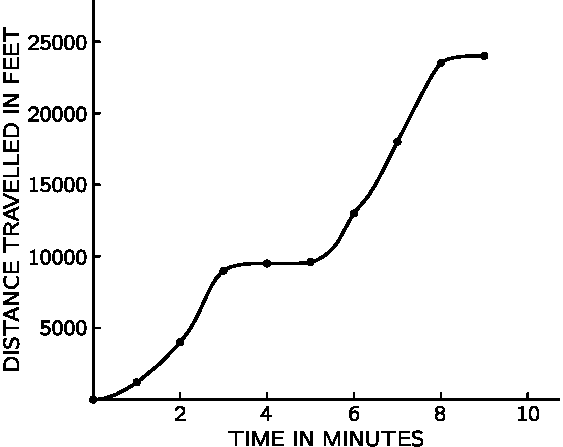
\includegraphics[width=0.3\textwidth]{fyz_fig098a.pdf}}
        \hspace{0.1\linewidth}                                                       \\
        \subfloat[ ]{\label{fyz:fig098b}
          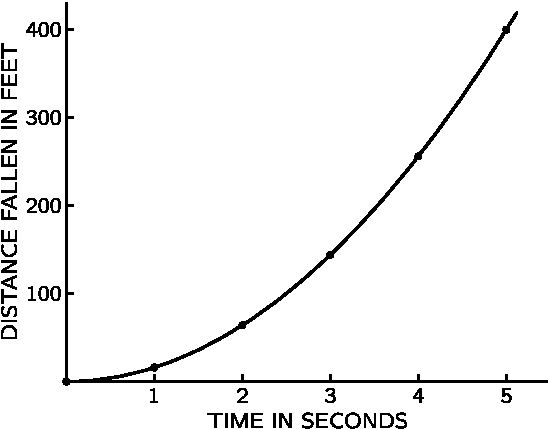
\includegraphics[width=0.3\textwidth]{fyz_fig098b.pdf}}
      \end{tabular}
      \caption{a) Graf závislosti autem ujeté vzdálenosti na čase b) Časová závislost vzdálenosti 
               padajícího tělesa  
               (\cite[s.~109]{Feynman01})}
      \label{fyz:fig098}
    \end{figure}


    Tento vztah nám umožňuje vypočítat vzdálenost v kterémkoli časovém okamžiku. Snad namítneme, že 
    by měl existovat vztah i pro první graf. Takový vztah je možné zapsat obecně ve tvaru
    \begin{equation}\label{FYZ:eq112}
      s = f(t),
    \end{equation}
    což znamená, že \(s\) je veličinou, která závisí na \(t\), nebo v matematickém jazyku je \(s\) 
    funkcí \(t\). Protože nevíme, jaká ta funkce je, nemůžeme ji vyjádřit v konkrétním algebraickém 
    tvaru.

    Poznali jsme dva příklady pohybu jež byly popsány velmi jednoduchým způsobem bez zvláštní 
    důmyslnosti. Avšak tyto příklady v sobě přece jen skrývají několik jemností. Především, co 
    rozumíme časem a prostorem? Ukazuje se, že jde o hluboké filozofické otázky, jež si ve fyzice 
    vyžadují důkladnou analýzu a ta nebývá snadná. Teorie relativity ukazuje, že představy prostoru 
    a času nejsou tak jednoduché, jak by se zdály na první pohled. Jenže zatím v našich prvních 
    úvahách nemusíme být příliš úzkostliví při definování těchto pojmů. Některým z nás se to bude 
    zdát divné, neboť jsme se učili, že ve vědě je třeba \emph{vše} přesně definovat. Jenže 
    \emph{vše} přesně definovat nemůžeme! Kdybychom se o to pokusili, dostali bychom se do podobné 
    situace jako ti dva filozofové, kteří v diskusi říkají jeden druhému: „Sám nevíte, o čem 
    hovoříte!“ Druhý odpovídá; ,A co to znamená \emph{vědět}? Co znamená \emph{hovořit}? Co znamená 
    \emph{sáni}?“ Abychom mohli hovořit konstruktivně, musíme se dohodnout, že mluvíme zhruba o 
    stejné věci. O čase už víme vše, co teď potřebujeme. Musíme si však být vědomi toho, že 
    existuje řada detailů, jež bude třeba prodiskutovat, ale to uděláme až později.
    
    Jednou z takových diskutabilních věcí je již uvedený fakt, že pozorovaný pohybující se bod se 
    vždy nachází na nějakém místě. (Samozřejmě, když na něj hledíme, je tam, ale bude tam i tehdy, 
    kdy se na něj nedíváme?) Ukazuje se, že v případě pohybujících se atomů není možné takto 
    uvažovat - na atomu si nemůžeme zvolit značku a pozorovat její pohyb. S tímto problémem se 
    setkáme v kvantové mechanice. Nejprve se však budeme zajímat o problémy, v nichž ještě 
    neuvažujeme takové komplikace, a až \emph{později} provedeme korekce, které si vynucují 
    nejnovější poznatky. Uspokojíme se proto s jednoduchým pohledem na čas a prostor. Víme, co tyto 
    pojmy v hrubých rysech představují a ti, kteří již řídili auto, vědí, co znamená rychlost.
    
  \section{Rychlost}
    Ačkoli zhruba víme, co „rychlost“ znamená, přece tu existují určité rafinované záludnosti; 
    vždyť jen uvažme, že učení Řekové nebyli schopni přiměřeně popsat problémy související s 
    rychlostí. Taková záludnost se objeví, když se snažíme přesně pochopit, co je třeba rozumět pod 
    „rychlostí“. Řekové z toho byli velmi zmateni a muselo být objeveno nové odvětví matematiky 
    (vedle geometrie a algebry Řeků, Arabů a Babylóňanů). Pro ilustraci problémů se pokusme řešit 
    tento problém jednoduchou algebrou: Balón nafukujeme tak, že jeho objem roste rychlostí 
    \SI{100}{\cubic\cm} za sekundu; jakou rychlostí roste jeho poloměr, když má balón 
    \SI{1000}{\cubic\cm}? Řeky jaksi zmátl takovýto problém zejména zásluhou některých úmyslně 
    matoucích Řeků. Aby poukázal na těžkosti související se studiem rychlosti, Zenon uvedl několik 
    paradoxů, ze kterých uvedeme jeden pro ilustraci problémů, jež se vyskytly při zkoumání pohybu. 
    V tomto paradoxu Zenon říká, že Achilles, ačkoli běží l0krát rychleji než želva, přece ji nikdy 
    nedoběhne. Argumentuje následujícím způsobem: „Předpokládáme-li, že na začátku běhu má želva 
    stometrový náskok, pak než Achilles uběhne \num{100} metrů a dostane se na místo, kde byla 
    původně želva, bude želva, která leze desetkrát pomaleji, \num{10} metrů před ním. Achilles 
    proto musí běžet dalších \num{10} metrů, aby želvu chytil, ale po deseti metrech zjistí, že 
    želva je \num{1} metr před ním. Když uběhne i ten metr, najde želvu \SI{10}{\cm} před sebou a 
    tak to půjde \emph{donekonečna}. Proto je v kterémkoli okamžiku želva před Achillem a ten ji 
    nikdy nedoběhne“. Co je na této argumentaci nesprávné? Je to skutečnost, že konečný čas se dělí 
    na nekonečně mnoho částí, právě tak jako konečná délka se dá rozdělit na nekonečně mnoho částí 
    opakovaným dělením dvěma. A tak, ačkoli (při této argumentaci) máme nekonečný počet kroků k 
    bodu, v němž Achilles dostihne želvu, neznamená to, že jde o nekonečně dlouhý \emph{časový} 
    interval. Na tomto příkladu je vidět, že při studiu rychlosti je možné narazit na problémy.
    
    Abychom si mohli ještě jasněji představit tyto problémy, připomeňme vtip o autě, které zastavil 
    policista. Nyní si představme, že v tomto autě sedí dáma a policista ji napomíná: „Paní, jela 
    jste rychlostí \num{90} km za hodinu!“ Dáma odpovídá: „To přece není možné, vždyť cestuji jen 
    sedm minut! Je to směšné -jak mohu jet rychlostí \num{90} km za hodinu, když jsem hodinu 
    nejela?“ Jak bychom odpověděli, kdybychom byli policistou? Samozřejmě, kdybychom skutečně byli 
    policistou, vše by bylo bez problémů. Prostě bychom té dámě řekli, že svoje argumenty může 
    přednést u soudu. Vyloučíme-li však takové řešení a uspokojíme se s poctivým intelektuálním 
    přístupem k tomuto problému, v němž chceme této dámě vysvětlit, co znamená jet rychlostí 
    \num{90} km za hodinu, co musíme udělat? Té dámě bychom vysvětlili, že kdyby pokračovala v 
    cestě a jela stále stejnou rychlostí, ujela by za hodinu \num{90} kilometrů. Mohla by však 
    namítnout: „Dala jsem nohu z plynu a auto zpomalovalo, a proto bych neujela \num{90} km, 
    kdybych takto pokračovala.“ Nebo uvažujme padající míček a předpokládejme, že bychom chtěli 
    znát jeho rychlost za dobu tří sekund, kdyby se dále pohyboval tak, jak se pohybuje nyní. 
    Znamenalo by to snad, že si udržuje \emph{zrychlení} a pohybuje se stále rychleji? Ne, 
    znamenalo by to, že si udržuje stejnou \emph{rychlost}. A to právě chceme definovat! Kdyby 
    totiž míček setrvával v původním pohybu, pohyboval by se tak, jak se pohybuje. Rychlost proto 
    musíme lépe definovat. Co se má vlastně zachovat? Ta dáma by také mohla argumentovat 
    následujícím způsobem: „Kdybych pokračovala v pohybu bez změny další hodinu, narazila bych do 
    zdi na konci ulice!“ Není tedy tak jednoduché říci, co vlastně máme na mysli.
    
    Mnozí fyzici zastávají názor, že měření je jedinou definicí kterékoli veličiny. Pak bychom, 
    samozřejmě, použili zařízení na měření rychlosti - \textbf{tachometr} - a upozornili bychom 
    dámu, že její tachometr ukazuje \num{90}. Dáma by však opět mohla namítat, že její tachometr je 
    pokažený a vůbec neukazuje. Znamená to ale, že se auto nepohybuje? Jsme přesvědčeni, že 
    existuje něco, čím je možné změřit rychlost dříve, než zkonstruujeme tachometr. Jen tehdy je 
    možné říci například: „Tachometr nepracuje správně“ nebo „tachometr je rozbitý“. Kdyby nebylo 
    možné měřit rychlost jinak než tachometrem, byla by tato věta nesmyslem. Máme tedy na mysli 
    něco, co je nezávislé na tachometru a tachometr slouží jen k měření této myšlenky. Uvažme, zda 
    je možné lépe definovat rychlost. Jako policista bychom řekli: „Milá paní, kdybyste jela 
    hodinu, narazila byste na zeď, ale kdybyste jela jednu sekundu, ujela byste \num{25} metrů. 
    Jela jste tedy rychlostí \num{25} metrů za sekundu a další sekundu byste ujela dalších \num{25} 
    metrů a ta zeď je mnohem dále.“ Dáma však namítá: „Neexistuje ale takový zákon, který by říkal, 
    že není dovoleno jet \num{25} metrů za sekundu! Zákon zakazuje jet \num{90} km za hodinu.“ Vy 
    potom řeknete, že je to přece totéž. Je-li to však totéž, pak by asi nedošlo k takové tahanici 
    o \num{25} metrů za sekundu. Padající míček se ve skutečnosti nemůže pohybovat stejně v průběhu 
    ani jedné sekundy, protože stále mění rychlost, a tak budeme muset rychlost nějak definovat.
    
    Zdá se, že se dostáváme na správnou stopu. Kdyby dáma pokračovala v cestě další tisícinu 
    hodiny, ujela by tisícinu z \num{90} km. Jinými slovy: nemusela by jet celou hodinu, důležité 
    je, že v \emph{daném okamžiku} jede takovou rychlostí. To znamená, že kdyby jela jen o nepatrný 
    okamžik déle, ujela by navíc takový úsek, jaký by ujelo auto jedoucí \emph{stálou} rychlostí 
    \num{90} km za hodinu. Myšlenka o \num{25} metrech za sekunduje možná správná; sledujeme, kolik 
    auto ujelo za poslední sekundu, dělíme to \num{25} metry a když dostaneme \num{1}, rychlost 
    byla \num{90} km za hodinu. Jinými slovy, rychlost můžeme zjistit tímto způsobem: zjistíme, jak 
    daleko dojdeme ve velmi krátkém čase, pak tuto vzdálenost dělíme časem, a tak dostaneme 
    rychlost. Čas je však třeba zvolit co nejkratší, neboť v průběhu tohoto času by se mohla stát 
    nějaká změna. Kdybychom v případě padajícího tělesa zvolili za takový časový interval hodinu, 
    bylo by to absurdní. Kdybychom zvolili jednu sekundu, dostali bychom docela dobrý výsledek v 
    případě auta, kdy je změna rychlosti malá, ale taková volba by nebyla dostatečná pro padající 
    těleso. Chceme-li zjistit rychlost co nejpřesněji, musíme zvolit časový interval co nejkratší. 
    Měli bychom tedy zvolit milióntinu sekundy a vzdálenost ujetou za tento čas dělit tou 
    milióntinou sekundy. Tak bychom dostali vzdálenost za sekundu, neboli to, co rozumíme jako 
    rychlost a takovýmto způsobem vlastně definujeme rychlost. Takto by bylo třeba odpovědět dámě v 
    automobilu, taková je definice, kterou budeme používat.
    
    Definice rychlosti obsahuje novou myšlenku, jež ve své obe\-cné podobě nebyla dostupná starým 
    Řekům. Tato myšlenka spočívá v tom, že uvažujeme \emph{nekonečné malou vzdálenost} a 
    odpovídající \emph{nekonečné malý čas}, uvedeme je do poměru a sledujeme chování tohoto poměru 
    při zmenšování časového intervalu. Jinak řečeno, zajímáme se o \textbf{limitu} ujeté 
    vzdálenosti dělenou odpovídajícím časem při \emph{nekonečném} zmenšování tohoto času. Na tuto 
    myšlenku přišli nezávisle na sobě Newton a Leibniz a představovala zrod nové matematické 
    disciplíny nazývané \textbf{diferenciální počet}. Tento počet vznikl v souvislosti s popisem 
    pohybu a jeho první aplikací byl vlastně náš problém související s otázkou: Co znamená jet 
    \uv{90 km/hod}?

    Pokusme se definovat rychlost trochu přesněji. Předpokládejme, že za krátkou dobu 
    \(\varepsilon\) urazí auto nebo jiné těleso krátkou vzdálenost \(x\). Pak definujeme rychlost 
    \(v\) jako
    \begin{equation}\label{FYZ:eq113}
      v = \frac{x}{\varepsilon}.
    \end{equation}
    přičemž přesnost bude tím větší, čím bude \(\varepsilon\) menší. Chceme-li to vyjádřit 
    matematicky, můžeme říci, že rychlost je limita podílu \(x/\varepsilon\) při \(\varepsilon\) 
    blížícím se k nule, tj.
    \begin{equation}\label{FYZ:eq114}
      v = \lim_{\varepsilon\to 0}{\frac{x}{\varepsilon}}.
    \end{equation}
    
    V případě dámy s autem nemůžeme provést totéž, neboť naše tabulka je neúplná. Víme jen to, kde 
    se dáma nachází na hranicích minutových intervalů. Proto si můžeme vytvořit jen přibližný obraz 
    o její rychlosti z toho, že například po dobu sedmé minuty ujela \num{1500} metrů, ale nevíme, 
    jaká byla její rychlost přesně na začátku sedmé minuty. Nevíme, zda zrychlovala a na začátku 
    šesté minuty měla rychlost \SI{1400}{\m/\min} a nyní má rychlost \SI{1600}{\m/\min}, nebo zda 
    pohyb probíhal jinak. Nevíme to proto, že nám chybí údaje uvnitř intervalu. Z takové tabulky 
    bychom mohli vypočítat rychlost jen tehdy, kdyby obsahovala nekonečně mnoho údajů. Máme-li však 
    matematický vztah úplný - takovým je v případě padajícího tělesa rovnice (\ref{FYZ:eq111}) - 
    můžeme vypočítat takovouto rychlost, neboť umíme určit polohu tělesa v kterémkoli časovém 
    okamžiku.
    
    Jako příklad si určíme rychlost padajícího tělesa v páté sekundě pádu. Jedním ze způsobů jak to 
    provést by mohlo být zkoumání \emph{tabulky} \ref{fyz:tab003}, z níž je vidět, že v páté 
    sekundě urazilo těleso \(125 - 80 = \SI{45}{\m}\). Proto by se zdálo, že těleso padalo 
    rychlostí \SI{45}{\m/\s}. To však není pravda, neboť rychlost se mění a ačkoli v tomto časovém 
    intervalu je to \emph{y průměru \SI{45}{\m/\s}}, těleso se zrychluje a na konci páté sekundy 
    padá rychleji než \SI{45}{\m/\s}. Chceme \emph{přesné určit jeho rychlost}. Je možné to udělat 
    následujícím způsobem: Víme, kde se těleso nacházelo v páté sekundě. V \SI{5.1}{\s} je podle 
    vztahu (\ref{FYZ:eq111}) vzdálenost, kterou těleso urazilo, rovna \(5\cdot5,1^2 = \SI{130.05} 
    {\m}\). V páté sekundě bylo těleso ve vzdálenosti \SI{125}{\m} a za další desetinu sekundy 
    urazilo \(\num{130.05} - \num{125} = \SI{5.05}{\m}\). Protože \SI{5.05}{\m} za \SI{0.1}{\s} je 
    totéž jako \SI{5.05}{\m\per\s}, zjistili jsme vlastně rychlost, ale ne zcela přesně. Nevíme, 
    je-li to rychlost v páté sekundě, v \SI{5.1}{\s} nebo \SI{5.05}{\s}, nebo někde mezi těmito 
    hodnotami. Měli jsme určit rychlost v \SI{5}{\s} a jestliže se nám to zcela nepodařilo, 
    zpřesníme náš postup. Vezmeme jednu tisícinu sekundy a vypočítáme, kam se až dostalo těleso. 
    Přidáme-li ještě tento čas k páté sekundě, dostaneme tedy v \SI{5.001}{\s}
    \begin{equation}\label{FYZ:eq115}
      s = 5\cdot5,001^2 = 5\cdot25,010001 = \SI{125.050005}{\m}.
    \end{equation}
    
    V poslední tisícině sekundy spadlo těleso \SI{0.050005}{\m} a dělíme-li toto číslo 
    \SI{0.001}{\s}, dostaneme rychlost \SI{50.005}{\m/\s}. Tento údaj je již přesnější, již je 
    docela blízký skutečnosti, ale přece jen není zcela přesný. Je však vidět, co musíme udělat, 
    chceme-li rychlost určit přesně. Bude užitečné formulovat úlohu trochu abstraktněji: Hledáme 
    rychlost v časovém okamžiku \(t_0\) Jenž v našem původním problému představoval \SI{5}{\s}. 
    Vzdálenost, do níž se dostalo těleso v čase \(t_0\) a kterou budeme označovat \(s_0\), je rovna 
    \(5t_0^2\) , tedy \SI{125}{\m} v našem případě. Při hledání rychlosti si klademe otázku: 
    \uv{Kde je těleso v čase \(t_{0+}\) (malý přírůstek) nebo \(t_0 + \varepsilon\)?} Nová poloha 
    je \(5(t_0 + \varepsilon)^2 = 5t_0^2 + 10t_0\varepsilon + 5\varepsilon^2\). Těleso je teď dále 
    než předtím, neboť nejprve bylo vzdáleno jen \(5t_0^2\) . Ta dodatečná vzdálenost je \(s_{0+}\) 
    (malý přírůstek) nebo \(s_0 + x\) (kde \(x\) je ten přírůstek). Odečteme-li od vzdálenosti 
    v čase \(t_0 + \varepsilon\) vzdálenost v \(ť_0\), dostaneme \(x\) - přírůstek vzdálenosti jako 
    \(x = 10t_0\varepsilon +5\varepsilon^2\). V prvním přiblížení bude rychlost rovna
    \begin{equation}\label{FYZ:eq116}
      v = \frac{x}{\varepsilon} = 10t_0 +5\varepsilon.
    \end{equation}
    
    Skutečná rychlost je hodnota tohoto poměru \(x/\varepsilon\) při nepatrném \(\varepsilon\). 
    Jinými slovy, po vytvoření poměru bereme \(\varepsilon\) vždy menší a menší, tj. blížící se k 
    nule. Rovnice pak přejde do tvaru \(v\)(v čase \(t_0\)) = \(10t_0\). V našem případě bylo \(t_0 
    = \SI{5}{\s}\), a proto \(v = 10\cdot5 = \SI{50}{\m/\s}\). Předtím, když jsme uvažovali 
    \(\varepsilon\) nejprve \SI{0.1}{\s} a podruhé \SI{0.001}{\s}, byla hodnota \(v\) trochu větší. 
    Nyní však vidíme, že skutečná rychlost je přesně \SI{50}{\m/\s}.
    
  \section{Rychlost jako derivace}
    Výpočet, který jsme právě provedli, je v matematice velmi častý a pro veličiny \(\varepsilon\) 
    a \(x\) se proto zavedlo speciální značení: Namísto \(\varepsilon\) se setkáme s \(\Delta t\) a 
    namísto \(x\) s \(\Delta s\). Pod \(\Delta t\) rozumíme \uv{malý přírůstek \(t\)}, který je 
    možné vždy zmenšovat. Přítomnost znaku \(\Delta\) neznamená násobení, právě tak jako 
    \(\sin\vartheta\) neznamená \(s\cdot i \cdot n \cdot \vartheta\). Jde prostě o časový přírůstek 
    a znak \(\Delta\) zvýrazňuje jeho zvláštní charakter. Podobnou vlastnost má \(\Delta s\), 
    rozdíl je jen v tom, že tentokrát jde o vzdálenost \(s\). Protože \(\Delta\) není součinitel, 
    nevykrátí se v poměru \(\Delta s/\Delta t\) a nedostaneme \(s/t\), právě tak, jako bychom 
    nedostali \(1/2\) z výrazu \(\sin \vartheta/\sin2\vartheta\). Při takovémto značení je 
    \emph{rychlost rovna limitě podílu \(\Delta s/\Delta t\) při \(\Delta t\) blížícím se k nule}, 
    tedy
    \begin{equation}\label{FYZ:eq117}
      \boxed{v = \lim_{\Delta t\to 0}{\frac{\Delta s}{\Delta t}}}\,.
    \end{equation}
    Tento výraz je stejný, jako vztah (\ref{FYZ:eq114}) s \(\varepsilon\) a \(x\), ale má tu 
    výhodu, že poukazuje na změnu určitých veličin a ukazuje co a jak se mění.
    
    Existuje ještě jeden zákon, který platí s dostatečnou přesností. Ten zákon říká, že vzdálenost 
    pohybujícího se bodu je možné vyjádřit jako součin rychlosti a časového intervalu, tj. \(\Delta 
    s = v\Delta t\). Tento zákon je správný tehdy, když se v průběhu uvažovaného časového intervalu 
    rychlost nemění, ale to obecně platí jen tehdy, kdy je \(\Delta t\) dostatečně malé. Fyzici 
    jsou zvyklí psát \(\dd{s} = v\dd{t}\), přičemž pod \(\dd{t}\) rozumějí \(\Delta t\) za 
    podmínek, v nichž je velmi malé. Při takovémto chápání je uvedený zákon dostatečně přesný. 
    Kdyby \(\Delta t\) bylo velké, mohla by se rychlost v průběhu tohoto intervalu měnit a přesnost 
    zákona by se zmenšila. Při \(\dd{t}\) blížícím se k nule je výraz \(\dd{s} = v\dd{t}\) zcela 
    přesný. Pomocí nově zavedených symbolů můžeme vztah (\ref{FYZ:eq117}) přepsat do tvaru
    \begin{equation}\label{FYZ:eq118}
      v = \lim_{\Delta t\to 0}{\frac{\Delta s}{\Delta t}} = \der{s}{t}.
    \end{equation}
    
    Veličina \(ds/dt\) se v tomto vztahu nazývá \uv{derivace s podle \(t\)} (takový název nám 
    připomíná, co se vlastně mění) a složitý proces hledání derivace se nazývá derivováním. 
    Objevují-li se \(ds\), \(dt\) samostatně, nazývají se \textbf{diferenciály}. Aby se nám stala 
    nová řeč bližší, připomeňme si, že již dříve jsme počítali derivaci funkce \(5t^2\), o níž jsme 
    zjistili, že je rovna \(10t\). Zvykneme-li si na novou řeč, budeme snadněji chápat mnohé 
    myšlenky. Abychom se pocvičili, vypočítáme derivaci složitější fimkce. Uvažujme vztah \(s = 
    At^3 + Bt+ C\), jenž by mohl popisovat pohyb bodu. Písmena \(A\), \(B\), \(C\), podobně jako ve 
    známém obecném tvaru kvadratické rovnice, představují konstantní čísla. Naším úkolem je najít 
    rychlost v kterémkoli okamžiku na základě tohoto vztahu. Abychom to provedli co nejelegantněji, 
    změníme \(t\) na \(t + \Delta t\), přičemž se změní \(s\) na \(s + \Delta s\) a \(\Delta s\) 
    vyjádříme pomocí \(\Delta t\) Tak dostaneme
    \begin{align}\label{FYZ:eq119}
     s + \Delta s &= A(t + \Delta t)^3 + B(t + \Delta t) + C    \nonumber \\
                  &= At^3 + Bt + C + 3At^2\Delta t + B\Delta t  \nonumber \\
                  &+ 3At(\Delta t)^2 + A(\Delta t)^3.
    \end{align}
    Protože \(s = At^3 + Bt + C\), můžeme psát
    \begin{equation}\label{FYZ:eq120}
         \Delta s = 3At^2\Delta t + B\Delta t + 3At(\Delta t)^2 + A(\Delta t)^3.
    \end{equation}

    \begin{table}      %\ref{fyz:tab005}
      \noindent\begin{tabular*}{\columnwidth}{@{\extracolsep{\stretch{1}}}*{2}{l}@{}}
        \toprule
        \small Funkce & \small Derivace \\
        \midrule
        \(s = t^n\)             & \(\der{s}{t} = nt^{n-1}\)                                      \\
        \(s=cu\)                & \(\der{s}{t} = c\der{u}{t}\)                                   \\
        \(s = u+v+w+\ldots\)    & \(\der{s}{t} = \der{u}{t} + \der{v}{t} + \der{w}{t} + \ldots\) \\
        \(s = c\)               & \(\der{s}{t} = 0\)                                             \\
        \(s = u^av^bw^c\ldots\) & \(\der{s}{t} = s\left(\frac{a}{u}\der{u}{t} + 
                                  \frac{b}{v}\der{v}{t} + \frac{c}{w}\der{w}{t} +\ldots\right)\) \\
        \bottomrule 
      \end{tabular*}
      \caption{Stručný přehled derivací: \(s\), \(u\), \(v\), \(w\) jsou libovolné funkce; \(t\), 
               \(a\), \(b\), \(c\), \(n\) jsou libovolné konstanty  
               (\cite[s.~114]{Feynman01})}
      \label{fyz:tab005}
    \end{table}
    
    Jenže my nepotřebujeme \(\Delta s\), ale \(\Delta s\) dělené \(\Delta t\). Proto předcházející 
    rovnici dělíme \(\Delta t\) a dostáváme
    \begin{equation}\label{FYZ:eq121}
       \frac{\Delta s}{\Delta t} = 3At^2 + B + 3At(\Delta t) + A(\Delta t)^2.
    \end{equation}
    Jde-li \(\Delta t\) k nule, je \(\frac{\Delta s}{\Delta t}\) rovno \(\der{s}{t}\) a platí
    \begin{equation}\label{FYZ:eq122}
       \frac{\Delta s}{\Delta t} = 3At^2 + B.
    \end{equation}
    
    To je základ derivování funkcí. Tento proces je ve skutečnosti ještě jednodušší, než by se na 
    první pohled zdálo. Všimněme si, že členy obsahující druhou nebo vyšší mocniny \(\Delta t\) je 
    možné zanedbat, neboť v limitě konvergují k nule.
    
    Po krátkém cvičení se celý proces pro nás stane ještě jednodušším, neboť budeme vědět, co je 
    třeba zanedbat. Existuje velmi mnoho pravidel derivování různých druhů funkcí. Tato pravidla je 
    možné si pamatovat, nebo je možné je vyhledat v tabulkách. Stručný seznam pravidel je uveden v 
    tab. \ref{fyz:tab005}.
  
  \newpage
  \section{Vzdálenost jako integrál}

    \begin{wraptable}[13]{r}{3.5cm}      %\ref{fyz:tab004}
      \centering
      \begin{tabular}{>{\centering\arraybackslash}p{2em}|>{\centering\arraybackslash}p{3em}}
        \hline  \(t\)    & \(v\)          \\
                 \si{\s} & \si{\m\per\s}  \\
         \hline  \num{0} & \num{0}        \\
                 \num{1} & \num{10}       \\
                 \num{2} & \num{20}       \\
                 \num{3} & \num{30}       \\
                 \num{4} & \num{40}       \\
        \hline 
      \end{tabular}
      \caption{Rychlost padajícího tělesa (\cite[s.~115]{Feynman01})}
      \label{fyz:tab004}
    \end{wraptable}
    Ještě nám zbývá analyzovat obrácenou úlohu. Předpokládejme, že místo tabulky vzdáleností máme 
    tabulku rychlostí v různých časech počínaje nulou. Pro padající kuličku jsou tyto rychlosti a 
    časy znázorněny v tab. \ref{fyz:tab004}. Podobnou tabulku je možné sestavit pro auto, 
    zaznamenáváme-li údaje tachometru každou minutu nebo každou půlminutu. Víme-li v každém časovém 
    okamžiku, jak rychle se auto pohybuje, můžeme určit, jak daleko se dostane? Tato úloha je 
    opakem úlohy, kterou jsme již vyřešili; je dána rychlost a chceme určit vzdálenost. Jak je 
    možné určit vzdálenost, známe-li rychlost? Není-li rychlost auta konstantní a dáma se chvíli 
    pohybuje rychlostí \SI{90}{\km\per\hour}, pak zpomalí, opět zrychlí atd., jak můžeme určit, kam 
    se až dostala? Je to jednoduché. Použijeme stejnou myšlenku jako v předcházejícím případě a 
    vyjádříme vzdálenost pomocí nekonečně malých částí. Jestliže mělo auto v první sekundě určitou 
    rychlost, můžeme ze vztahu \(\Delta s = v\Delta t\) vypočítat, kam až se auto při dané 
    rychlosti v první sekundě dostalo. V další sekundě se rychlost auta liší o málo; kam se auto 
    dostalo, vypočítáme tak, že vynásobíme novou rychlost časem. Takto dostáváme jistý počet malých 
    vzdáleností a celková vzdálenost bude součtem těchto malých vzdáleností. To znamená, že 
    vzdálenost bude součtem součinů rychlostí a časů, tedy \(s=\sum v\Delta t\), kde řecké písmeno 
    \(\sum\) (sigma) označuje součet. Pro přesnost je třeba poznamenat, že v součtu vystupují 
    rychlosti v určitém okamžiku, např. \(i\)-tém časovém okamžiku a jsou násobeny \(\Delta t\), tj.
    \begin{equation}\label{FYZ:eq123}
      s = \sum_{i}v(t_i)\Delta t.
    \end{equation}
    Tyto časové okamžiky vyhovují následující podmínce: \(t_{i+1} = t_i + \Delta t\). Ani takovémto 
    způsobem určovaná vzdálenost nebude přesná, neboť v průběhu časového intervalu \(\Delta t\) se 
    může rychlost měnit. K zabezpečení přesnosti musíme časové intervaly brát co nejkratší. 
    Skutečné \(s\) je
    \begin{equation}\label{FYZ:eq124}
      s = \lim_{\Delta t\to0}\sum_{i}v(t_i)\Delta t.
    \end{equation}
    Pro takovouto limitu zavedli matematici speciální symbol analogický symbolu pro diferenciál.    
    \(\Delta\) přechází v \(d\) a zvýrazňuje tak skutečnost, že čas je co nejmenší, o rychlosti 
    hovoříme jako o \(v\) v čase \(t\) a součet píšeme s trochu deformovaným velkým „S“ \(\int\) 
    (podle latinského slova \emph{summa}), kterému se dnes říká bohužel jen znak integrálu. Máme 
    tedy
    \begin{equation}\label{FYZ:eq125}
      \boxed{s = \int\sum_{i}v(t_i)\Delta t}\,.
    \end{equation}
    
    Proces sčítání takových výrazů se nazývá \textbf{integrování} a představuje \emph{opak} 
    derivování. Derivace tohoto integrálu je \(v\), takže jeden operátor (\(d\)) ruší druhý 
    (\(\int\)). Vzorce pro integrování je možné získat ze vzorců pro derivování jejich obrácením, 
    neboť jsou vzájemně inverzní. Každý si může sestavit svou tabulku integrálů, bude-li derivovat 
    všechny druhy funkcí. Z každého diferenciálního vzorce dostaneme integrální, když ho obrátíme.
    
    Každou funkci je možné derivovat analyticky, tj. operace probíhá algebraicky a vede k určité 
    funkci. S integrálem je to však jinak a není možné napsat analytický tvar pro libovolný 
    integrál. Je sice možné ho vypočítat, například tak, že nejprve provedeme uvedenou sumaci, a 
    zjemníme-li dostatečně interval \(\Delta t\), dostaneme výsledek téměř přesně. Máme-li však 
    danou určitou funkci, nemůžeme obecně nalézt analytický výraz pro její integrál. Vždy se můžeme 
    pokusit najít funkci, která nám po zderivování dá požadovanou funkci. Jenomže taková funkce 
    nemusí existovat v tom smyslu, že by se dala vyjádřit pomocí funkcí, které již dostaly nějaké 
    pojmenování.
    
  \section{Zrychlení}
    Dalším krokem na cestě k pohybovým rovnicím je zavedení veličiny, která přesahuje pojem 
    rychlosti a souvisí se \emph{změnou} rychlosti pohybu. K takovéto veličině přicházíme, když si 
    klademe otázku, jak se \emph{mění} rychlost. V předcházejících kapitolách jsme hovořili o 
    případech, v nichž síly způsobovaly změny rychlosti. Určitě jsme již slyšeli vzrušující zprávy 
    o autech, která za \num{10} sekund dosáhnou z klidu rychlosti \SI{100}{km\per\hour}. Na 
    takovémto příkladu je vidět, jak se mění rychlost - ale jen v průměru. V dalším stádiu se 
    budeme zabývat složitějším problémem - rychlostí změny rychlosti. Jinými slovy, o kolik metrů 
    za sekundu se změní rychlost v průběhu sekundy, tj. o kolik metrů za sekundu za sekundu. Již 
    dříve jsme odvodili vztah pro rychlost padajícího tělesa v podobě \(v= 10 t\), který je 
    zaznamenán v tab. \ref{fyz:tab004}, a nyní bychom chtěli zjistit, jak se rychlost mění za 
    sekundu. Veličinu vyjadřující tuto změnu nazýváme \textbf{zrychlením}.
    
    Zrychlení je definováno jako časová změna rychlosti. Z předcházející diskuze již víme dost k 
    tomu, abychom mohli zapsat zrychlení jako derivaci \(\der{v}{t}\), podobně, jako rychlost byla 
    časovou derivací vzdálenosti. Derivujeme-li vztah \(v= 10t\), dostaneme zrychlení padajícího 
    tělesa
    \begin{equation}\label{FYZ:eq101}
      a = \der{v}{t} = 10.
    \end{equation}
    
    (Při derivování výrazu \(10t\)l jsme využili výsledek získaný v předcházející úloze, kde jsme 
    zjistili, že derivace \(Bt\) je prostě \(B\) tedy konstanta. Položením \(B=10\) dostaneme 
    okamžitě výsledek, že derivace \(10t\) je \num{10}) To znamená, že rychlost padajícího tělesa 
    roste každou sekundu o \SI{10}{\m\per\s}. Tato skutečnost je zřejmá i z tab. 8.4. Tento příklad 
    je velmi jednoduchý, ale zrychlení obecně nebývají konstantní. Příčinou konstantního zrychlení 
    v případě padajícího tělesa je skutečnost, že na něj působí konstantní síla a podle Newtonova 
    zákona je zrychlení úměrné síle.
    
    Jako další příklad si všimněme zrychlení v úloze, kterou jsme již vyřešili, když jsme se 
    zabývali rychlostí. Když jsme vycházeli ze vztahu \(s = At^3 + Bt + C\), dostali jsme pro 
    \(v=\der{s}{t}\) vyjádření
    \begin{equation}\label{FYZ:eq102}
      v = 3At^2 + B.
    \end{equation}
    
    Protože zrychlení je časová derivace rychlosti, musíme poslední výraz derivovat. Připomeňme si 
    pravidlo, podle něhož je derivace dvojčlenu rovna součtu derivací jednotlivých členů. Abychom 
    při derivování prvního členu nemuseli opakovat celý základní proces, připomeňme si, že 
    kvadratický člen jsme již derivovali při derivování funkce a výsledek byl takový, že koeficient 
    se zdvojnásobil a t2 se změnilo na t. Proto budeme předpokládat, že totéž se děje i v tomto 
    případě. Derivace \(3At^2\) proto bude \(6At\). Dále musíme derivovat \(B\), tedy konstantní 
    člen. Podle předcházejícího pravidla je však derivace \(B\) rovna nule, a tak tento člen 
    nepřispívá ke zrychlení. Konečný výsledek je proto \(a=\der{v}{t}= 6At\).
    
    Uveďme ještě dva užitečné vztahy, jež je možné získat integrací. Pohybuje-li se těleso 
    vycházející z klidu s konstantním zrychlením \(g\), jeho rychlost v libovolném čase \(t\) je
    \begin{equation}\label{FYZ:eq103}
      v = gt.
    \end{equation}
    Vzdálenost, kterou těleso až do tohoto okamžiku urazí, je
    \begin{equation}\label{FYZ:eq104}
      v = \frac{1}{2}gt^2.
    \end{equation}
    
    Pro zápis derivace se používají různá matematická značení. Protože rychlost je \(ds/dt\) a 
    zrychlení je časová derivace rychlosti, můžeme psát i
    \begin{equation}\label{FYZ:eq105}
      a = \der{ }{t}\left(\der{s}{t}\right) = \dder{s}{t},
    \end{equation}
    což představuje běžný zápis druhé derivace.
    
    Existuje i jiný zákon, podle něhož je rychlost rovna integrálu zrychlení. To je právě opakem 
    vztahu \(a = \der{v}{t}\). Protože jsme již zjistili, že vzdálenost je integrálem rychlosti, 
    můžeme vzdálenost najít \emph{dvojnásobnou integrací zrychlení}.
    
    \begin{figure}[ht!]  %\ref{fyz:fig099}
      \centering
      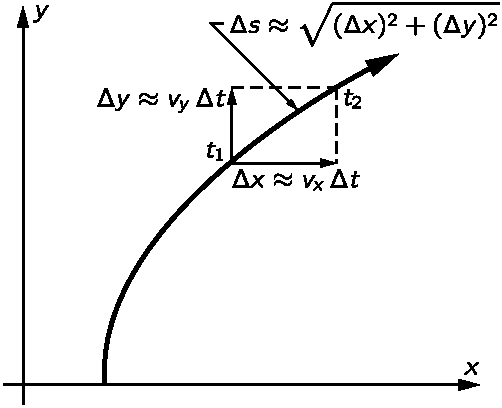
\includegraphics[width=0.7\linewidth]{fyz_fig099.pdf}
      \caption{Popis pohybu tělesa v rovině a výpočet jeho rychlosti
               (\cite[s.~118]{Feynman01})}
      \label{fyz:fig099}
    \end{figure}
    Předcházející diskuze se zabývala jen jednorozměrným pohybem a nedostatek místa nám dovoluje 
    jen velmi stručnou analýzu trojrozměrného pohybu. Uvažujme částici P, která se pohybuje 
    libovolně v trojrozměrném prostoru. Na začátku této kapitoly jsme jednorozměrný pohyb 
    ilustrovali pohybem auta a sledovali jsme vzdálenost, kterou auto ujede za různou dobu od 
    počátečního bodu. Pak jsme hovořili o rychlosti jako o časové změně ujeté vzdálenosti a o 
    zrychlení jako o časové změně rychlosti. Podobně je možné zkoumat trojrozměrný pohyb. 
    Jednodušší však bude znázornit si pohyb nejprve na dvojrozměrném grafu a výsledky pak zobecnit 
    na trojrozměrný případ. Zvolme si dvojici navzájem kolmých souřadnicových os a polohu částice v 
    kterémkoli časovém okamžiku určíme odměřením jeho vzdálenosti od každé ze souřadnicových os. 
    Každá poloha je tedy určena \(x\)-ovou a \(y\)-ovou vzdáleností a pohyb je možné popsat pomocí 
    tabulky, v níž jsou tyto vzdálenosti zapsány jako funkce času. (Rozšíření tohoto procesu na 
    trojrozměrný případ si vyžaduje jen zavedení další osy, kolmé na předcházející osy, a měření 
    třetí, \(z\)-ové, vzdálenosti. Vzdálenosti se potom neměří od souřadnicových os, ale od 
    souřadnicových \emph{rovin}.)
    
    Jak můžeme určit rychlost, máme-li sestavenou tabulku s \(x\)-ovými a \(y\)-ovými vzdálenostmi? 
    Nejprve najdeme složky rychlosti v jednotlivých směrech. Horizontální složka rychlosti, tj. 
    \(x\)-ová složka, je časovou derivací \(x\)-ové vzdálenosti, tedy
    \begin{equation}\label{FYZ:eq106}
      v_x = \der{x}{t}.
    \end{equation}
    Podobně vertikální složka rychlosti, tj. \(y\)-ová složka je
    \begin{equation}\label{FYZ:eq108}
      v_y = \der{y}{t}.
    \end{equation}
    V trojrozměrném případě máme ještě
    \begin{equation}\label{FYZ:eq107}
      v_z = \der{z}{t}.
    \end{equation}
    
    Jak můžeme určit rychlost podle skutečné dráhy pohybu, známe-li složky rychlosti? V 
    dvojrozměrném případě uvažujme dvě následující polohy částice lišící se o krátkou vzdálenost 
    \(\Delta s\) a krátký časový interval \(t_2- t_1 = \Delta t\). V čase \(\Delta t\) urazí 
    částice horizontálně vzdálenost \(\Delta x \approx  v_x\Delta t\) a vertikálně vzdálenost 
    \(\Delta y \approx  v_y\Delta t\) (Symbol \uv{\(\approx\)} znamená „přibližně“.) Skutečná 
    uražená vzdálenost je podle obr. \ref{fyz:fig099} rovna přibližně
    \begin{equation}\label{FYZ:eq109}
      \Delta s = \sqrt{(\Delta x)^2 + (\Delta y)^2}.
    \end{equation}
    Přibližnou rychlost v průběhu časového intervalu získáme dělením tohoto výrazu \(\Delta t\). 
    Přibližuje-li se \(\Delta t\), podobně jako na začátku kapitoly, k nule, získáme pro rychlost 
    vyjádření
    \begin{equation}\label{FYZ:eq110}
      v = \der{s}{t} = \sqrt{(\der{x}{t})^2 + (\der{y}{t})^2} = \sqrt{v_x^2 + v_y^2}
    \end{equation}
    a v trojrozměrném případě
    \begin{equation}\label{FYZ:eq097}
      v = \sqrt{v_x^2 + v_y^2 + v_z^2}.
    \end{equation}

    Podobně, jako jsme definovali rychlosti, můžeme definovat zrychlení: \(x\)-ová složka zrychlení 
    \(a_x\) je derivací \(v_x\)-ové složky rychlosti (tj. \(a_x = \dder{x}{t}\) je druhou derivací 
    \(x\) podle času) a analogicky definujeme ostatní složky zrychlení.

    Uvažujme jeden pěkný příklad složeného pohybu v rovině. Nechť se kulička pohybuje horizontálně 
    konstantní rychlostí \(u\) a nechť současně vertikálně padá s konstantním zrychlením \(-g\). 
    Jaký je to vlastně pohyb? Víme, že \(\der{x}{t} = v_x = u\). Protože rychlost \(v\) je 
    konstantní
    \begin{equation}\label{FYZ:eq100}
      x = ut,
    \end{equation}

    \begin{wrapfigure}[12]{r}{5cm}  %\ref{fyz:fig100}
      \centering
      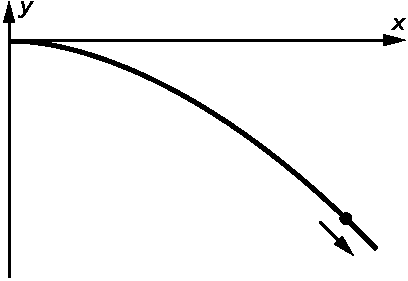
\includegraphics[width=0.7\linewidth]{fyz_fig100.pdf}
      \caption{Parabola, již opisuje padající těleso, které má počáteční horizontální rychlost
               (\cite[s.~119]{Feynman01})}
      \label{fyz:fig100}
    \end{wrapfigure}
    a protože při pohybu dolů je zrychlení \(-g\) konstantní, je možné vzdálenost \(y\) padajícího 
    předmětu zapsat ve tvaru
    \begin{equation}\label{FYZ:eq098}
      y = -\frac{1}{2}gt^2.
    \end{equation}
    
    Jak vypadá křivka takovéhoto pohybu, tj. jaký je vztah mezi \(y\) a \(x\)? Z rovnice 
    (\ref{FYZ:eq098}) můžeme vyloučit čas, neboť \(t= x/u\). Po této substituci dostaneme
    \begin{equation}\label{FYZ:eq099}
      y = -\frac{g}{2u^2}x^2.
    \end{equation}
    Tento vztah mezi \(x\) a \(y\) je možné považovat za rovnici trajektorie pohybující se kuličky. 
    Vyneseme-li závislost do grafu, získáme křivku, jež se nazývá \textbf{parabola} (obr. 
    \ref{fyz:fig100}). Jakékoli padající těleso vystřelené v libovolném směru se bude pohybovat po 
    parabole. 
  
  \newpage
  \section{Příklady a cvičení}
    %---------------------------------------------------------------
      % !TeX spellcheck = cs_CZ
  
Nyní si demonstrujeme užití pohybových rovnic při popisu trajektorie, libovolného bodu na 
železničním kole, které se odvaluje po kolejnici \textbf{bez} smyku. Na obrázku \ref{fyz:fig142} 
vidíme, že železniční kola jsou opatřena \emph{okolky}, která slouží jako bezpečnostní prvek proti 
vykolejení a pro hladký průjezd kolejových spojek, výhybek apod. Úlohu můžeme formulovat pro různé 
body, které mají vzdálenost od středu kola menší, větší, nebo rovnou poloměru nákolku. Otázka zní, 
jak bude jejich trajektorie rozvinutá v čase vypadat.

\begin{figure}[ht!]  %\ref{fyz:fig142}
  \centering
  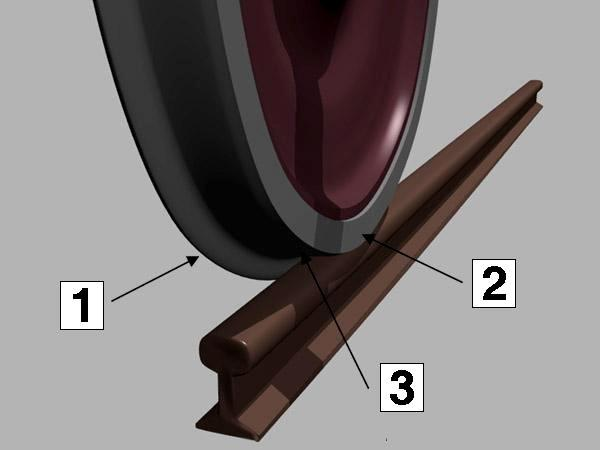
\includegraphics[width=0.5\linewidth]{fyz_fig142.jpg}
  \caption{Nákres železničního kola s částí kolejnice: \(1\ldots\text{okolek}\), \(2\ldots 
          \text{nákolek}\), \(3\ldots\text{plocha odvalování}\), kredit: \wikiOkolek. K příkladu 
          \ref{fyz:exam003}.}
  \label{fyz:fig142}
\end{figure}

\wikitextrule
\begin{example}\label{fyz:exam003}
  Kolo vagónu se valí po vodorovné kolejnici. Uvažujme bod, který je v počátečním okamžiku pod 
  středem kola ve vzdálenosti, která může být menší, rovna nebo větší než vzdálenost středu kola od 
  kolejnice.

   {\centering
    \captionsetup{type=figure}
    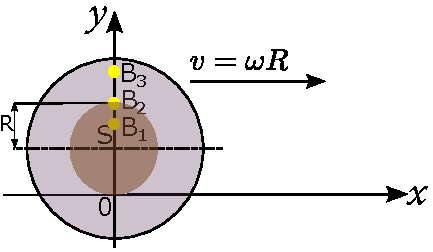
\includegraphics[width=0.6\linewidth]{fyz_fig141.pdf}
    \captionof{figure}{Kolo vagónu a tři možné polohy bodu}
    \label{fyz:fig141}
  \par}
  \vspace{0.5em}
  Určeme parametrické rovnice dráhy zvoleného bodu, složky rychlosti a její velikost, složky 
  zrychlení a jeho velikost, tečné a normálové zrychlení a poloměr křivosti dráhy. 
  \cite[p.~11]{Slavik}
  \vspace{1em}
  \newline
  \textbf{Řešení}: Obvodová rychlost v místě dotyku s kolejnicí je \(v=\omega R\), což vzhledem k 
  předpokladu o valení představuje posuvnou rychlost kola. Parametrické rovnice pro střed kola jsou pak
  \begin{subequations}\label{mech:eq_wheel_center}
    \begin{align}
      x_s &= \omega R t \\
      y_s &= R
    \end{align}
  \end{subequations}

   {\centering
    \captionsetup{type=figure}
    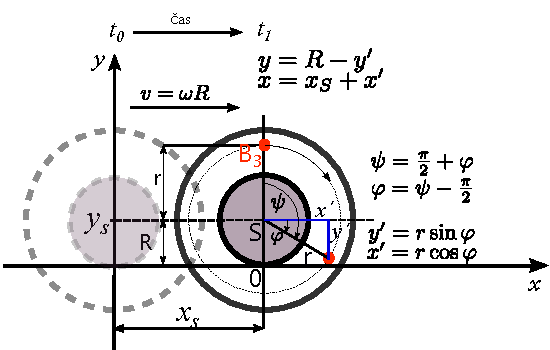
\includegraphics[width=0.9\linewidth]{fyz_fig143.pdf}
    \captionof{figure}{Náčrt pro odvození parametrických rovnic pohybu libovolně zvoleného bodu na 
               kole vagónu}
    \label{fyz:fig143}
  \par}
  \vspace{0.5em}
  Uvažovaný bod \(B_3\) na obr. \ref{fyz:fig143} je ve své nové pozici v čase \(t_1\) posunut vůči 
  středu o vzdálenost \(r\cdot\sin\omega t\) ve směru osy \(x\) a o vzdálenost \(r\cdot\cos\omega 
  t\) ve směru osy \(y\). Z obrázku \ref{fyz:fig143} lze odvodit následující rovnice pro souřadnice 
  libovolného bodu \(B\) na kole vagónu.
  
           
    \begin{itemize}
      \item ve směru osy \(x\):
      \begin{align*}
        x &= x_s + x'                        \\
        x &= x_s + r\cos(\psi-\frac{\pi}{2}) \\
        x &= x_s + r\sin\psi                 \\
        x &= \omega R t + r\sin\omega t
      \end{align*}
      \end{itemize}  


   \begin{itemize}
      \item ve směru osy \(y\): 
      \begin{align*}
        y &= y_s - y'                        \\
        y &= y_s - r\sin(\psi-\frac{\pi}{2}) \\
        y &= y_s + r\cos\psi                 \\
        y &= R + r\cos\omega t
      \end{align*}
    \end{itemize}

  takže, parametrické rovnice dráhy mají tvar \textbf{cykloidy}:
  \begin{equation*}
    x = \omega R t + r\sin\omega t  \qquad y = R + r\cos\omega t
  \end{equation*}
  \begin{itemize}
    \item Složky rychlosti:
      \begin{align*} 
       v_x &= \frac{dx}{dt} = \omega R + r\omega\cos\omega t                       \\
       v_y &= \frac{dy}{dt} = -r\omega\sin\omega t                                 \\
       v   &= \sqrt{v_x^2 + v_y^2}= \omega\sqrt{R^2 + 2Rr\cos\omega t + r^2}
      \end{align*}
    \item Složky zrychlení:
      \begin{align*}
        a_x &= \frac{dv_x}{dt} = -r\omega^2\sin\omega t                           \\
        a_y &= \frac{dv_y}{dt} = -r\omega^2\cos\omega t                           \\
        a   &= \sqrt{a_x^2 + a_y^2}= r\omega^2\sqrt{\sin^2\omega t + 
               \cos^2\omega t} = r\omega^2
      \end{align*}
      Tento výsledek je superpozicí rovnoměrného kruhového a rovnoměrného přímočarého pohybu.
    \item \textbf{Tečné zrychlení} \(a_t\) dostaneme derivací velikosti rychlosti
      \begin{equation*}
        a_t = \frac{dv}{dt} = -\cdot\frac{2Rr\omega^2\sin\omega t }{2\sqrt{R^2 + 
                2Rr\cos\omega t + r^2}}
      \end{equation*}
    \item \textbf{Normálové zrychlení} \(a_n\) získáme užitím Pythagorovy věty
      \begin{align*}
        a_n &= \sqrt{a^2 - a_t^2}                                                 \\
        a_n &= \sqrt{(r\omega^2)^2-\left(
               \frac{Rr\omega^2\sin\omega t}
                    {\sqrt{R^2 + 2Rr\cos\omega t + r^2}}\right)^2}
      \end{align*}
    \item \textbf{Poloměr křivosti} $R_0$ dostaneme ze vztahu $a_n=\frac{v^2}{R_0}$:
      \begin{equation*}
          R_0 =  \dfrac{\omega^2\cdot(R^2 + 2Rr\cos\omega t + r^2)}{\sqrt{r^2\omega^4 - 
                   \dfrac{R^2r^2\omega^4\sin^2\omega t}{R^2 + 2Rr\cos\omega t + r^2}}}
      \end{equation*}
      Poloměr křivosti není roven vzdálenosti od středu kola r: drahou bodu není kružnice, nýbrž 
      cykloida (viz obr. \ref{fyz:fig140}). Pokud bod pevně spojený s kružnicí leží na 
      jejím obvodu, pak při valení této kružnice po přímce opisuje tento bod \textbf{prostou} 
      (obecnou) cykloidu. 
  \end{itemize}
  
  \begin{align*}
    (x - \omega R t)^2            &= r^2\sin^2\omega t                          \\
    (y-R)^2                       &= r^2\cos\omega t                            \\
    (x - \omega R t)^2 + (y-R)^2  &= r^2\sin^2\omega t + r^2\cos\omega t        \\
    (x - \omega R t)^2 + (y-R)^2  &= r^2 \quad                                  \\
    \shortintertext{kde \(t = \frac{1}{\omega}\arccos\frac{y-R}{r}\)}
    \Aboxed{\left(x - R\arccos\frac{y-R}{r}\right)^2 + (y-R)^2  &= r^2}
  \end{align*}

   {\centering
    \captionsetup{type=figure}
 %   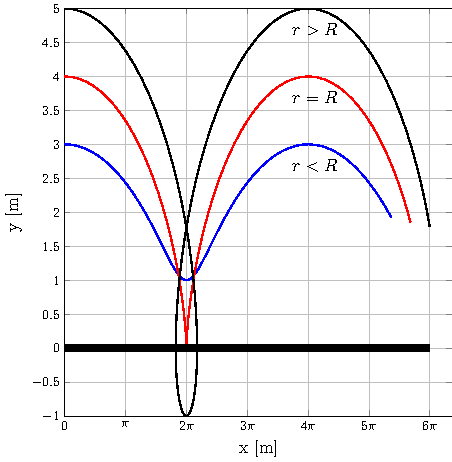
\includegraphics[width=0.8\linewidth]{fyz_fig140.pdf}
    \input{../src/FYZ/img/fyz_fig140.tex}
    \captionof{figure}{Cykloida: pro $B_2\ldots r=R$ je cykloida prostá; $B_3\ldots r>R$
              cykloida prodloužená; $B_1\ldots r<R$ cykloida zkrácená; \texttt{[cykloida.m]} }
    \label{fyz:fig140}
    \par}       
    \vspace{1em}
   
   Z obrázku \ref{fyz:fig140} je také patrné, že pokud bod pevně spojený s kutálející se kružnicí 
   neleží na obvodu této kružnice, ale jeho vzdálenost od středu kružnice o poloměru \(R\)  je 
   \(r\) , pak pro \(r<R\) získáme \textbf{cykloidu zkrácenou} a pro \(r>R\)  \textbf{cykloidu 
   prodlouženou}.
      
%---------------------------------------------------------------
\lstinputlisting[language=Matlab]{../src/FYZ/matlab/cicloid.m}
\begin{lstlisting}[caption= Výpočet křivky cykloidy pro pro tři různé body.]
\end{lstlisting}
%---------------------------------------------------------------

%    %---------------------------------------------------------------
%      \tikzexternaldisable
%      \input{../src/FYZ/img/fyz_fig144.tex}
%      \tikzexternalenable
%    %---------------------------------------------------------------
    
\end{example}
\wikitextrule

    %---------------------------------------------------------------

} %tikzset
%---------------------------------------------------------------------------------------------------
\printbibliography[heading=subbibliography]
\addcontentsline{toc}{section}{Seznam literatury} 
%==== Kapitola: Newtonovy zákony dynamiky ==========================================================
% !TeX spellcheck = cs_CZ
%{\tikzset{external/prefix={tikz/FYZI/}}
% \tikzset{external/figure name/.add={ch07_}{}}
%---------------------------------------------------------------------------------------------------
% file fey1ch09.tex
%---------------------------------------------------------------------------------------------------
%================ Kapitola: Newtonovy zákony dynamiky =============================================
\setchaptertoc
\chapter{Newtonovy zákony dynamiky}\label{fyz:IchapIX}

  \section{Hybnost a síla}\label{fyz:IchapIXsecI}
    Objev zákonů dynamiky neboli zákonů pohybu, byl dramatickým momentem v historii vědy. Ještě 
    před Newtonem byly pohyby takových objektů, jako jsou planety, záhadou, ale po Newtonovi se 
    stalo vše pochopitelným. Dokonce bylo možné spočítat i malé odchylky od Keplerových zákonů 
    podmiňované působením jiných planet. Po Newtonově objevu bylo možné plně analyzovat pohyb 
    kyvadla, kmity závaží zavěšeného na pružině a jiné jevy. Tak je to i s touto kapitolou: před ní 
    jsme neuměli vypočítat, jak se pohybuje závaží upevněné na pružině a tím méně vypočítat vliv 
    Jupiteru a Saturnu na pohyb Uranu. Po této kapitole budeme schopni vypočítat nejen pohyb 
    kmitajícího závaží, ale i poruchy pohybu Uranu způsobované Jupiterem a Saturnem!
    
    Galileo udělal veliký krok na cestě za pochopením pohybu svým objevem \textbf{principu 
    setrvačnosti}: \emph{Je-li předmět ponechán sám sobě bez vnějších vlivů, pokračuje v přímočarém 
    pohybu konstantní rychlostí, jak se původně pohyboval, nebo zůstává nehybný, jak původně stál.} 
    Taková situace se samozřejmě nikdy neobjevuje v přírodě a postrčíme-li předmět na stole, 
    zastaví se. Zastaví se proto, že nebyl ponechán sám sobě - tře se totiž o stůl. Nalezení tohoto 
    zákona vyžadovalo značnou představivost a tu měl právě Galileo.
    
    Abychom se však dostali dále, musíme znát zákon, podle něhož předměty \emph{mění} svou 
    rychlost, jestliže \emph{jsou} něčím ovlivňovány. To udělal Newton. Newton zformuloval tři 
    zákony. První zákon byl jen opakováním uvedeného Galileova principu setrvačnosti. Druhý zákon 
    určuje, jak se mění rychlost v důsledku různých vlivů nazývaných \textbf{silami}. Třetí zákon 
    do určité míry popisuje síly, ale o tomto zákoně budeme hovořit jindy. Nyní si budeme všímat 
    Newtonova druhého pohybového zákona, který udává, jak síla ovlivňuje pohyb nějakého objektu a 
    říká, že \emph{změna veličiny zvané hybnost za jednotku času je úměrná síle}. Později toto 
    tvrzení stručné matematicky zapíšeme, ale nejprve vysvětlíme jeho podstatu.
    
    \textbf{Hybnost} není totéž, co rychlost Ve fyzice používáme mnoho slov a každé z nich má 
    přesný význam, ačkoli v každodenní běžné řeči se takováto přesnost nevyžaduje. Nyní se 
    zamysleme nad definicí hybnosti. Zatlačíme-li rukou na nějaký lehký předmět, snadno ho uvedeme 
    do pohybu. Zatlačíme-li stejně na mnohem těžší předmět, bude se pohybovat mnohem pomaleji. 
    Namísto slov „lehký“ a „těžký“ však musíme používat výrazy s \emph{menší hmotností} a 
    \emph{větší hmotnosti} neboť mezi tíhou a setrvačností předmětu je rozdíl, který musíme brát v 
    úvahu. (Jak těžké je uvést předmět do pohybu a jakou má tíhu, to jsou dvě rozdílné věci.) Tíha 
    a setrvačnost jsou \emph{úměrné} a na zemském povrchu je často považujeme za číselně stejné, a 
    právě to vyvolává u některých studentů rozpaky. \emph{Na Marsu by se tíha předmětů lišila od 
    jejich tíhy na Zemi, ale množství síly potřebné na překonání setrvačnosti by se nezměnilo}.
    
    Termín \textbf{hmotnost} používáme jako \textbf{kvantitativní míru setrvačnosti}. Hmotnost 
    můžeme měřit například tak, že zavěšeným předmětem budeme kroužit určitou rychlostí a budeme 
    měřit sílu, která je potřebná k jeho udržení v otáčivém pohybu. Takovýmto způsobem můžeme 
    každému předmětu přisoudit určitou hmotnost. \emph{Hybnost} předmětu je součinem dvou faktorů: 
    jeho \emph{hmotnosti} a jeho \emph{rychlosti}. Druhý Newtonův zákon je proto možné zapsat v 
    matematickém tvaru
    \begin{equation}\label{fyz:eq052}
      \vec{F} = \der{}{t}(m\vec{v}).
    \end{equation}
    
    K tomu je třeba uvést několik poznámek. Při zápisu takového zákona se opíráme o mnoho 
    intuitivních myšlenek, náznaků a předpokladů, jež v prvním stádiu zkombinujeme přibližně do 
    našeho „zákona“. Později se můžeme vrátit zpět a detailně zvážit význam každého členu. 
    Pokusíme-li se však o to příliš brzy, můžeme se dostat do rozpaků. Proto budeme pro začátek 
    považovat některé věci za samozřejmé. Budeme předpokládat, že hmotnost předmětu je 
    \emph{konstantní}. Hmotnost ve skutečnosti konstantní není, ale začneme s Newtonovou aproximací 
    konstantní, po celou dobu neměnné hmotnosti a dále budeme předpokládat, že předmět vytvořený 
    složením dvou předmětů má hmotnost rovnou součtu jejich hmotností. Newton při sestavování své 
    rovnice z těchto předpokladů vycházel, vždyť jinak by jeho rovnice neměla smysl. Představme si 
    třeba, že hmotnost se mění nepřímo úměrně rychlosti. Pak by se hybnost za \emph{žádných 
    okolností neměnila}. Zákon má smysl jen tehdy, když víme, jak se hmotnost mění s rychlostí. 
    Proto zatím předpokládáme, že hmotnost se \emph{nemění}.
    
    Dále si musíme podrobněji všimnout \emph{síly}. V hrubé představě ji považujeme za zatlačení 
    nebo zatáhnutí, které provedou naše svaly, ale když máme k dispozici pohybový zákon, můžeme 
    sílu definovat přesněji. Nejdůležitější co si musíme uvědomit, je skutečnost, že tento zákon 
    nezahrnuje jen změny velikosti hybnosti nebo rychlosti, ale i změny jejich \emph{směru}. Je-li 
    hmotnost konstantní, rovnici (\ref{fyz:eq052}) je možné napsat ve tvaru
    \begin{equation}\label{fyz:eq053}
      \boxed{
        \vec{F} = m\der{\vec{v}}{t} = m\vec{a}.
       }
    \end{equation}
    
    \textbf{Zrychlení} a představuje změnu rychlosti za jednotku času a Newtonův druhý pohybový 
    zákon říká více než to, že účinek síly se mění nepřímo úměrně hmotnosti. Říká i, že směr změny 
    rychlosti a směr síly jsou shodné. Proto si musíme uvědomit, že změna rychlosti, neboli 
    zrychlení, má širší význam než v hovorové řeči. Rychlost pohybujícího se předmětu se může měnit 
    tak, že se jeho pohyb zrychluje, zpomaluje, nebo se mění směr pohybu. Zrychlení kolmé na směr 
    rychlosti jsme uvažovali v kapitole \ref{fyz:chap_fey_gravity}. Tam jsme viděli, že předmět 
    pohybující se po kružnici s poloměrem \(R\) rychlostí \(v\) se vychyluje od přímočaré dráhy o 
    vzdálenost \(\frac{1}{2}\frac{v^2}{R}t\), je-li \(t\) velmi malé. Proto vztah pro zrychlení 
    kolmé na směr pohybuje
    \begin{equation}\label{fyz:eq059}
      a = \frac{v^2}{R}.
    \end{equation}
    
    Síla působící ve směru kolmém k rychlosti vyvolá proto pohyb předmětu po zakřivené dráze, jejíž 
    poloměr křivosti můžeme získat tak, že sílu dělíme hmotností předmětu (tak dostaneme zrychlení) 
    a pak použijeme vztah (\ref{fyz:eq059}).
    
  \section{Směr a velikost rychlosti}\label{fyz:IchapIXsecII}
    Abychom upřesnili náš jazyk, musíme se hlouběji zamyslet nad pojmem rychlost V hovorové řeči se 
    se slovem rychlost setkáváme často. Takto používaný pojem má však chudší obsah než pojem 
    \emph{rychlost} používaný ve fyzice.

    \begin{figure}[ht!]  %\ref{fyz:fig056}
      \centering
      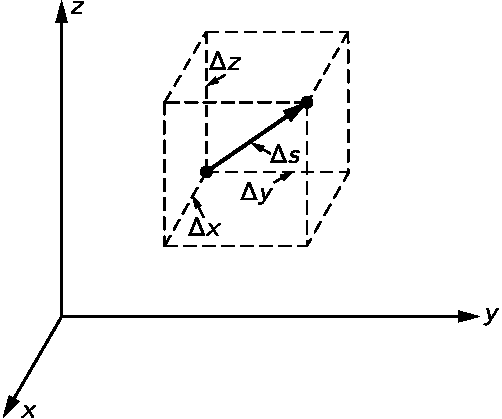
\includegraphics[width=0.6\linewidth]{fyz_fig056.pdf}
      \caption{Malé posunutí předmětu (\cite[s.~124]{Feynman01})}
      \label{fyz:fig056}
    \end{figure}
    
    Rychlost jako fyzikální veličina znamená určitou velikost, tj. jistý počet metrů za sekundu, 
    ale i směr, v němž se uskutečňuje pohyb, zatímco v hovorové řeči znamená jen velikost. 
    Matematicky můžeme vystihnout velikost i směr rychlosti, určíme-li, jak se souřadnice \emph{x, 
    y, z} daného předmětu mění s časem. Nechť se například v určitém časovém okamžiku předmět 
    pohybuje tak, jak je znázorněno na obr. \ref{fyz:fig056}. V malém časovém intervalu \(\Delta 
    t\) urazí jistou vzdálenost \(\Delta x\) ve směru osy \(x\), \(\Delta y\) ve směru \(y\) a 
    \(\Delta z\) ve směru osy \(z\). Výsledkem těchto tří změn souřadnic je posunutí \(\Delta s\) 
    podél úhlopříčky rovnoběžnostěnu se stranami \(\Delta x\), \(\Delta y\), \(\Delta z\). Posunutí 
    \(\Delta x\) je součin x-ové složky rychlosti a intervalu \(\Delta t\) a podobné vztahy platí 
    pro \(\Delta y\), \(\Delta z\)
    \begin{equation}\label{fyz:eq060}
      \Delta x = v_x\Delta t,\quad \Delta y = v_y\Delta t,\quad \Delta z = v_z\Delta t.
    \end{equation}
    
  \section{Složky rychlosti, zrychlení a síly}\label{fyz:IchapIXsecIII}
    Vztah (\ref{fyz:eq060}) představuje rozklad rychlostí na složky, které nám udávají, jak rychle 
    se předmět pohybuje ve směru osy \(x\), \(y\), a \(z\). Velikost i směr rychlosti budou plně 
    určeny, udáme-li číselné hodnoty jejich tří kolmých složek
    \begin{equation}\label{fyz:eq061}
      v_x = \der{x}{t}, v_y = \der{y}{t}, v_z = \der{z}{t}
    \end{equation}

    \begin{figure}[ht!]  %\ref{fyz:fig057}
      \centering
      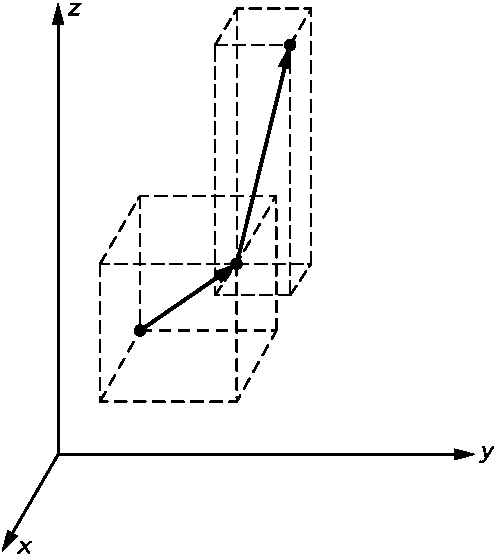
\includegraphics[width=0.5\linewidth]{fyz_fig057.pdf}
      \caption{Změna rychlosti, při níž se mění její velikost i směr (\cite[s.~125]{Feynman01})}
      \label{fyz:fig057}
    \end{figure}
    
    Přitom velikost rychlosti předmětu je
    \begin{equation}\label{fyz:eq062}
      \der{s}{t} = \abs{v} = \sqrt{v^2_x + v^2_y + v^2_z}. 
    \end{equation}
    
    Nyní předpokládejme, že působením síly mění rychlost svůj směr a velikost tak, jak je to 
    znázorněno na obr. \ref{fyz:fig057}. Tuto zdánlivě složitou situaci vyřešíme poměrně snadno, 
    určíme-li změny složek rychlosti. Změna složky rychlosti ve směru osy \(x\) za čas \(\Delta t\) 
    je \(\Delta v_x = a_x\Delta t\), přičemž \(a_x\) je x-ová složka zrychlení. Podobně je \(\Delta 
    v_y = a_y\Delta t\), \(\Delta v_z = a_z\Delta t\). Vidíme, že Newtonův druhý pohybový 
    zákon tím, že hovoří o shodnosti směru síly a zrychlení, představuje vlastně tři zákony. Každá 
    ze složek síly ve směrech \(x, y, z\) je totiž rovna součinu hmotnosti a časové změny 
    odpovídající složky rychlosti.
    \begin{subequations}\label{fyz:eq063}
      \begin{align}
        F_x &= m\der{v_x}{t} = m\dder{x}{t} = ma_x, \\
        F_y &= m\der{v_y}{t} = m\dder{y}{t} = ma_y, \\
        F_z &= m\der{v_z}{t} = m\dder{z}{t} = ma_z. 
      \end{align}
    \end{subequations}
    
    Podobně jako rychlost a zrychlení je možné i sílu rozložit na složky promítnutím úsečky rovné 
    absolutní hodnotě síly a ukazující směr působení síly na souřadnicové osy \(x, y, z\):
    \begin{subequations}\label{fyz:eq064}
      \begin{align}
        F_x &= F\cos(x,F),\\
        F_y &= F\cos(y,F),\\
        F_z &= F\cos(z,F).
      \end{align}
    \end{subequations}

    Pod \(F\) rozumíme velikost síly a \((x, F)\) představuje úhel, jenž svírá osa \(x\) se směrem 
    síly atd.
    
    Rovnice (\ref{fyz:eq063}) představují úplnou podobu Newtonova druhého pohybového zákona. 
    Známe-li síly působící na předmět a rozložíme je na jednotlivé složky, můžeme z těchto rovnic 
    určit pohyb předmětu. Uvažujme jednoduchý příklad. Nechť ve směrech \(y\) a \(z\) nepůsobí 
    síly. Jediná síla nechť působí například vertikálně ve směru osy \(x\). Vztah (\ref{fyz:eq063}) 
    říká, že rychlost se bude měnit jen ve vertikálním směru a v horizontálním směru bude zůstávat 
    stálá. To jsme již viděli v případě speciálního zařízení z kapitoly \ref{fyz:chap_fey_gravity} 
    (obr. \ref{fyz:fig058}). Padající těleso se pohybuje tak, že jeho horizontální pohyb se nemění 
    a ve vertikálním směru se pohyb uskutečňuje tak, jako kdyby horizontální pohyb neexistoval. 
    Jinak řečeno, pohyby ve směrech \(x\), \(y\), \(z\) jsou nezávislé, jsou-li složky sil vzájemně 
    nezávislé.
    
  \section{Co je to síla?}\label{fyz:IchapIXsecIV}
    Chceme-li využít Newtonovy zákony, musíme znát matematické vyjádření síly; Newtonovy zákony 
    totiž takříkajíc \emph{zaměřují naši pozornost na síly}. Pohybuje-li se předmět zrychleně, musí 
    na něj něco působit a my musíme toto působení odhalit. Naším budoucím programem v dynamice bude 
    \emph{hledání zákonů platných pro síly}. Sám Newton nám poskytl několik příkladů. Objevil zákon 
    síly všeobecné gravitace. V případě jiných sil nám poskytl alespoň částečnou informaci 
    prostřednictvím svého třetího zákona, který budeme studovat v další kapitole a který hovoří o 
    rovnosti akce a reakce.
    
    Rozšiřme náš předcházející příklad a zajímejme se o síly působící na předmět v blízkosti 
    zemského povrchu. U Země je síla ve vertikálním směru, způsobovaná přitažlivostí, úměrná 
    hmotnosti předmětu a je téměř nezávislá na výšce, jde-li o výšky malé ve srovnání se zemským 
    poloměrem \(R\). Tato síla je rovna \(F= \kappa mM/R^2 = mg\), kde \(g = \kappa M/R^2\) se 
    nazývá \textbf{gravitační zrychlení}. Gravitační zákon nám tedy říká, že tíha je úměrná 
    hmotnosti; tato síla má vertikální směr a je rovna součinu hmotnosti a gravitačního zrychlení. 
    Opět zjišťujeme, že v horizontálním směru jde o pohyb s konstantní rychlostí. Zajímavým pohybem 
    je právě pohyb ve vertikálním směru a pro tento pohyb vyplývá z druhého Newtonova zákona
    \begin{equation}\label{fyz:eq126}
      mg=\left(\dder{x}{t}\right).
    \end{equation}
    
    \luagraphic[0.8]{fyz_fig101.pdf}{Závaží na pružině (\cite[s.~127]{Feynman01})}{fyz:fig101}

    Vykrátíme-li \(m\), zjistíme, že zrychlení ve směru \(x\) je konstantní a je rovno \(g\). To je 
    známý zákon volného pádu pod vlivem gravitace, který vyjadřují rovnice
    \begin{align}
      v_x &= v_0 + gt                       \nonumber \\
        x &= x_0 + v_0t + \frac{1}{2}gt^2.  \label{fyz:eq127}
    \end{align}
    
    Nyní si všimněme dalšího příkladu. Předpokládejme, že jsme sami schopni zkonstruovat zařízení na
    obr. \ref{fyz:fig101}, jež vyvolává sílu úměrnou výchylce od rovnováhy a směřující proti této 
    výchylce. Takovým zařízením je \emph{pružina}. Nebudeme si všímat gravitace, jež je 
    vykompenzována počátečním napnutím pružiny, ale budeme se zajímat jen o \emph{nadbytečné} síly. 
    Pak zjistíme, že taháme-li závaží směrem dolů, pružina ho zvedá, a tlačíme-li závaží nahoru, 
    pružina ho tlačí dolů. Zařízení bylo pečlivě navrženo tak, aby síla byla tím větší, čím více 
    stlačíme závaží nahoru, a to přesně přímo úměrně výchylce od rovnovážné polohy, a podobně 
    nahoru působící síla je úměrná našemu vychýlení závaží směrem dolů. Při sledování dynamiky 
    tohoto zařízení vidíme zajímavý pohyb: nahoru, dolů, nahoru, dolů... Vzniká otázka, zda 
    Newtonovy rovnice popisují tento pohyb správně. Zkusme přesně vypočítat takovýto periodický 
    pohyb pomocí Newtonova zákona (\ref{fyz:eq063}). V našem případě máme
    \begin{equation}\label{fyz:eq128}
      -kx = m\left(\der{v_x}{t}\right).
    \end{equation}
    Jde o situaci, kdy se rychlost ve směru osy \(x\) mění úměrně výchylce \(x\). Nemá smysl teď 
    pracovat s tolika konstantami, a tak si situaci zjednodušíme předpokladem, že se buď změnilo 
    časové měřítko, nebo se změnily jiné jednotky, takže shodou okolností \(k/m = 1\). Pak dostaneme
    \begin{equation}\label{fyz:eq129}
      \der{v_x}{t} = -x.
    \end{equation}
    Abychom mohli pokračovat, musíme zjistit, co je to \(v_x\); jenže my už víme, že je to rychlost 
    změny polohy v čase.
    
  \section{Smysl dynamických rovnic}\label{fyz:IchapIXsecV}
    Pokusme se nyní zjistit, co znamená rovnice (\ref{fyz:eq129}). Nechť v daném časovém okamžiku 
    \(t\) má předmět určitou rychlost \(v\) a polohu \(x\). Jaká bude jeho rychlost a poloha v 
    trochu pozdějším okamžiku \(t+\varepsilon\)? Dokážeme-li odpovědět na tuto otázku, vyřešíme náš 
    problém, neboť vycházíme-li z daných počátečních podmínek, dokážeme určit změny v prvním 
    okamžiku, pak v dalším a dalším a postupně určíme celý vývoj pohybu. Kvůli konkrétnosti 
    předpokládejme, že v čase \(t = 0\) je \(x= 1\) a \(v_x = 0\). Proč se předmět vůbec pohybuje? 
    Protože na něj v kterékoli poloze s výjimkou \(x=0\) působí síla. Je-li \(x > 0\), působí síla 
    směrem nahoru. Proto rychlost, která byla zpočátku nulová, se bude v souladu s pohybovým 
    zákonem měnit. Jakmile začne rychlost růst, předmět se začíná pohybovat nahoru. V libovolném 
    časovém okamžiku \(t\) můžeme při velmi malém \(\varepsilon\) vyjádřit polohu v čase \(t + 
    \varepsilon\) pomocí polohy a rychlosti v čase \(t\) s dostatečnou přesností následujícím 
    způsobem
    \begin{equation}\label{fyz:eq130}
      x(t+\varepsilon) = x(t) + \varepsilon v_x(t).
    \end{equation}
    
    Čím je \(\varepsilon\) menší, tím přesnější je tento výraz, ale i tehdy, kdy \(\varepsilon\) 
    není zanedbatelně malé, je tento výraz ještě přijatelně přesný. Co je možné nyní říci o 
    rychlosti? Abychom mohli stanovit rychlost v čase \(t + \varepsilon\) musíme zjistit, jak se 
    rychlost mění, tj. musíme zjistit \emph{zrychlení}. Jak najdeme zrychlení? V tom nám pomohou 
    zákony dynamiky. Podle nich je zrychlení v naší úloze rovno \(-x\)\footnote{V námi zvolených 
    jednotkách.}. Proto
    \begin{subequations}
      \label{fyz:eq131} 
      \begin{align}
        v_x(t+\varepsilon) &= v_x(t) + \varepsilon a_x(t)  \label{fyz:eq131a}        \\
                           &= v_x(t) - \varepsilon x(t)    \label{fyz:eq131b}
      \end{align}
    \end{subequations} 
    
    Rovnice (\ref{fyz:eq131a}) je jen \emph{kinematická} a říká, že rychlost se mění v důsledku 
    přítomnosti zrychlení. Rovnice (\ref{fyz:eq131b}) je však \emph{dynamická}, neboť dává do 
    souvislosti zrychlení a sílu. Poukazuje na to, že v daném časovém okamžiku můžeme v naší 
    konkrétní úloze nahradit zrychlení výrazem \(-x(t)\). Známe-li tedy v daném čase \(x\) i \(v\), 
    známe i zrychlení, jež nám umožní určit novou rychlost a novou polohu. Takto pracuje 
    \emph{dynamický mechanizmus}. Rychlost se trochu změní v důsledku působení síly a i poloha se 
    trochu změní v důsledku rychlosti.
     
  \section{Numerické řešení rovnic}\label{fyz:IchapIXsecVI}
    Pusťme se nyní do skutečného řešení naší úlohy. Zvolíme třeba \(\varepsilon = \num{0.100}\) 
    sekundy. Provedeme-li všechny výpočty a uvidíme, že \(\varepsilon\) nebylo dost malé, můžeme se 
    vrátit a výpočty provádět s \(\varepsilon = \SI{0.010}{\s}\). Ptáme se, jaké je 
    \(x(\num{0.1})\), vycházíme-li z počáteční hodnoty \(x(0) = \num{1.00}\). Bude rovno původní 
    poloze \(x(0)\) zvětšené o rychlost (která je nulová) násobenou \SI{0.10}{\s}. Proto je 
    \(x(0,1)\) stále rovno \num{1.00}, neboť pohyb ještě nezačal. Nová rychlost v čase 
    \SI{0.10}{\s} bude rovna původní rychlosti \(v(0) = 0\) zvětšené o součin \(\varepsilon\) a 
    zrychlení. Zrychlení je \(-x(0) = \num{-1.00}\). Je tedy
    \begin{align*}
      v(\num{0.1}) &= \num{0.00} - \num{0.10}\cdot\num{1.00} = -\num{0.10}. \\ 
      \shortintertext{V čase \SI{0.20}{\s} máme}
      x(\num{0.2}) &= x(0,1) + \varepsilon v(0,1)   \\
                   &= \num{1.00} - \num{0.10}\cdot\num{0.10} = \num{0.99}   \\
      \shortintertext{a dále}
      v(\num{0.2}) &= v(0,1) + \varepsilon a(0,1)   \\
                   &= -\num{0.10} - \num{0.10}\cdot\num{1.00} = -\num{0.20}
    \end{align*}
    V tomto procesu můžeme pokračovat, a tak vypočítat celý pohyb, což je naším úkolem. V praxi 
    však používáme určité triky, které nám umožní zvětšit přesnost. Kdybychom pokračovali v začatém 
    postupu, získali bychom jen přibližný obraz o pohybu, neboť \(\varepsilon= \SI{0.100}{\s}\) je 
    jen velmi hrubý krok. Pro zvýšení přesnosti bychom museli zvolit velmi malý interval, např. 
    \num{0.01}. Abychom tak prošli dostatečné dlouhý časový interval, museli bychom provést velké 
    množství početních cyklů. Práci si proto zorganizujeme tak, abychom zvýšili přesnost výpočtu 
    při původním intervalu \(\varepsilon= \SI{0.10}{\s}\). Toho lze dosáhnout rafinovaným zlepšením 
    metody analýzy.

    Všimněme si, že nová poloha je vlastně stará poloha zvětšená o součin intervalu a rychlosti. 
    \emph{Jakému časovému okamžiku} však přísluší tato rychlost? Na začátku a na konci časového 
    intervalu máme jiné rychlosti. Naše zlepšení bude spočívat v tom, že vezmeme rychlost \emph{ze 
    středu intervalu}. Známe-li původní rychlost, jež se mění, pak nemůžeme dostat správnou 
    odpověď, když počítáme jen s původní rychlostí. Musíme proto použít jakousi střední rychlost 
    mezi začátkem a koncem intervalu. Stejné úvahy platí i pro rychlost: Abychom určili změny 
    rychlosti, musíme použít zrychlení v čase odpovídajícím středu mezi dvěma časovými okamžiky, v 
    nichž rychlost určujeme. Proto rovnice, které budeme používat, budou následující: Pozdější 
    poloha je rovna předcházející poloze zvětšené o \(\varepsilon\)-násobek rychlosti \emph{v čase, 
    jenž leží ve středu intervalu}. Podobně rychlost v tomto středním bodě je rychlost v čase o 
    \(\varepsilon\) menším (to je střed předcházejícího intervalu) zvětšená o 
    \(\varepsilon\)-násobek zrychlení v čase \(t\).
    
    Používáme tedy rovnice
    \begin{subequations}
      \label{fyz:eq132} 
      \begin{align}
      x(t+\varepsilon) 
           &= x(t) + \varepsilon v\left(t+\frac{\varepsilon}{2}\right), \label{fyz:eq132a} \\
      v(t+\frac{\varepsilon}{2}) 
           &= v\left(t-\frac{\varepsilon}{2}\right) + \varepsilon a(t), \label{fyz:eq132b} \\
      a(t) &= -x(t).                                                    \label{fyz:eq132c}
      \end{align}
    \end{subequations}
    
    Zbývá již jen jeden malý problém: co je \(v(\frac{\varepsilon}{2})\)? Na začátku jsme měli 
    \(v(0)\) a ne \(v(-\frac{\varepsilon}{2})\). Abychom mohli zahájit výpočet, použijeme 
    doplňující rovnici \(v(\frac{\varepsilon}{2}) = v(0) + (\frac{\varepsilon}{2})a(0)\).
    
    Teď již máme k výpočtu vše připraveno. Je vhodné použít zápis výpočtu v podobě tabulky se 
    sloupci pro čas, polohu, rychlost a zrychlení, s posunutými řádky pro rychlost, jak to 
    znázorňuje tab. \ref{fyz:tab006}. Taková tabulka je samozřejmě, jedním z vhodných způsobů 
    zápisu výsledků z  rovnic (\ref{fyz:eq132}) a tyto rovnice vlastně zcela nahrazuje. Zaplňujme 
    postupně její jednotlivá místa údaji.
    
    
    \begin{figure}[ht!]  %\ref{fyz:fig102}
      \centering
      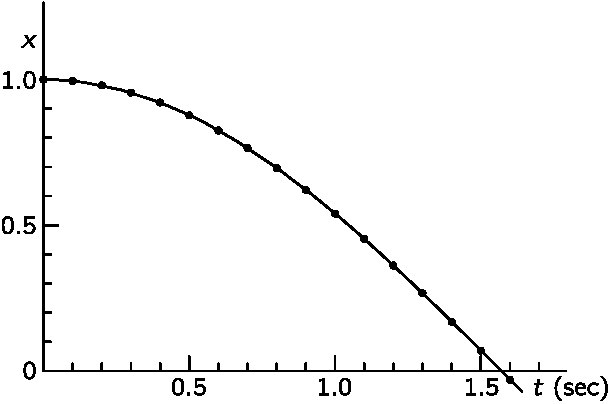
\includegraphics[width=0.6\linewidth]{fyz_fig102.pdf}
      \caption{Graf pohybu závaží na pružině (\cite[s.~129]{Feynman01})}
      \label{fyz:fig102}
    \end{figure}
    
    Tabulka nám poskytuje velmi dobrou představu o pohybu: Pohyb začíná z klidu, pak závaží získává 
    malou rychlost směrem nahoru (zápornou) a zmenšuje se vzdálenost od rovnovážné polohy. 
    Zrychlení je pak sice trochu menší, ale ještě stále se zvyšuje rychlost. Rychlost se však 
    zvyšuje stále méně a méně, až při přechodu bodem \(x = 0\) přibližně v čase \(t = 
    \SI{1.5}{\s}\) dojde k opačnému pohybu: poloha \(x\) bude záporná a zrychlení tedy kladné. 
    Rychlost se zmenšuje. Bude zajímavé porovnat údaje v tabulce s funkcí \(x = \cos t\). Takové 
    porovnání najdeme na obr. \ref{fyz:fig102}. Je vidět shoda s našimi výpočty s přesností na tři 
    platné číslice! Později uvidíme, že \(x = \cos t\) je přesné matematické řešení naší pohybové 
    rovnice. Uvedený postup ukazuje sílu numerické analýzy, která takovým jednoduchým výpočtem 
    poskytla přesné výsledky.
    
    \begin{table}[ht!]      %\ref{fyz:tab006}
      \centering
      \scalebox{0.8}{
      \begin{tabular}{|>{\centering\arraybackslash}p{3em}|>{\centering\arraybackslash}p{4em}
                      |>{\centering\arraybackslash}p{4em}|>{\centering\arraybackslash}p{4em}|}
        \hline  
         \(t\) & \(x\) & \(v_x\)  & \(a_x\)     \\
        \hline
           \num{0.0} &  \num{1.000} & \multirow{2}{*}{\num{-0.050}} & \num{-1.000} \\ 
           \num{0.1} &  \num{0.995} & \multirow{2}{*}{\num{-0.150}} & \num{-0.995} \\
           \num{0.2} &  \num{0.980} & \multirow{2}{*}{\num{-0.248}} & \num{-0.980} \\
           \num{0.3} &  \num{0.955} & \multirow{2}{*}{\num{-0.343}} & \num{-0.955} \\
           \num{0.4} &  \num{0.921} & \multirow{2}{*}{\num{-0.435}} & \num{-0.921} \\
           \num{0.5} &  \num{0.877} & \multirow{2}{*}{\num{-0.523}} & \num{-0.877} \\
           \num{0.6} &  \num{0.825} & \multirow{2}{*}{\num{-0.605}} & \num{-0.825} \\
           \num{0.7} &  \num{0.764} & \multirow{2}{*}{\num{-0.682}} & \num{-0.764} \\
           \num{0.8} &  \num{0.696} & \multirow{2}{*}{\num{-0.751}} & \num{-0.695} \\
           \num{0.9} &  \num{0.621} & \multirow{2}{*}{\num{-0.814}} & \num{-0.621} \\
           \num{1.0} &  \num{0.540} & \multirow{2}{*}{\num{-0.868}} & \num{-0.540} \\
           \num{1.1} &  \num{0.453} & \multirow{2}{*}{\num{-0.913}} & \num{-0.453} \\
           \num{1.2} &  \num{0.362} & \multirow{2}{*}{\num{-0.949}} & \num{-0.362} \\
           \num{1.3} &  \num{0.267} & \multirow{2}{*}{\num{-0.976}} & \num{-0.267} \\
           \num{1.4} &  \num{0.169} & \multirow{2}{*}{\num{-0.993}} & \num{-0.169} \\
           \num{1.5} &  \num{0.070} & \multirow{2}{*}{\num{-1.000}} & \num{-0.070} \\
           \num{1.6} & \num{-0.030} &                               & \num{-0.030} \\
        \hline 
      \end{tabular}}
      \caption{Řešení rovnice \(\der{v_x}{t} = -x\), interval \(\varepsilon = \SI{0.1}{\s}\)  
               (\cite[s.~130]{Feynman01})}
      \label{fyz:tab006}
     \end{table}

  \section{Pohyb planet}\label{fyz:IchapIXsecVII}
    Předcházející analýza je velmi vhodná k popisu kmitající stru\-ny. Nás však zajímá, zda je 
    takto 
    možné analyzovat i pohyb planet kolem Slunce. Zjistíme, je-li možné v jistém přiblížení dospět 
    k eliptické oběžné dráze. Budeme předpokládat, že Slunce je nekonečně těžké v tom smyslu, že 
    nemusíme uvažovat jeho pohyb. Dále předpokládejme, že planeta začala svůj pohyb na určitém 
    místě a pohybuje se určitou rychlostí kolem Slunce po nějaké křivce. Pomocí Newtonových 
    pohybových zákonů a gravitačního zákona se pokusíme zjistit, jaká je to křivka. Jak to 
    provedeme? V daném okamžiku je planeta v určitém bodě v prostoru. Označíme-li \(r\) radiální 
    vzdálenost od Slunce k tomuto bodu, pak víme, že na planetu působí síla směřující ke Slunci, 
    která je podle gravitačního zákona rovna konstantě násobené součinem hmotností Slunce a planety 
    a dělené druhou mocninou jejich vzdálenosti. K dalším úvahám potřebujeme vědět, jaké zrychlení 
    vyvolává tato síla. Potřebujeme znát složky zrychlení ve dvou směrech, jimiž vedeme osy \(x\) a 
    \(y\) (počátek umístíme v Slunci). Poloha planety v daném okamžiku je určena souřadnicemi \(x\) 
    a \(y\) (o souřadnici \(z\) předpokládáme, že je stále nulová, neboť v tom směru nepůsobí žádná 
    síla, a jestliže počáteční rychlost \(v_z\) byla nulová, není důvod, aby se souřadnice 
    změnila). Gravitační síla směřuje podél spojnice planety a Slunce, jak je vidět na obr. 
    \ref{fyz:fig103}.

    \luagraphic[0.8]{fyz_fig103.pdf}{Gravitační síla působící na planetu 
    (\cite[s.~131]{Feynman01})}{fyz:fig103}

    Z uvedeného obrázku je vidět, že horizontální složka síly souvisí s celkovou silou stejným 
    způsobem, jakým horizontální souřadnice \(x\) souvisí s celkovou délkou přepony \(r\), neboť 
    příslušné trojúhelníky jsou podobné. Dále, je-li \(x\) kladné, bude \(F_x\) záporné. Je \(F_x = 
    -\abs{F}x/r\), tedy \(F_x = -\abs{F}x/r = -\kappa Mmx/r^3\). Využijme nyní dynamického zákona 
    (\ref{fyz:eq063}), z něhož vyplývá, že \(x\)-ová nebo \(y\)-ová složka zrychlení násobená 
    hmotností planety je rovna \(x\)-ové resp. \(y\)-ové složce síly. Tak dostaneme rovnice
    \begin{subequations}\label{fyz:eq133}
      \begin{align} 
        m\left(\der{v_x}{t}\right) &= -\frac{\kappa Mmx}{r^3}, \label{fyz:eq133a}   \\
        m\left(\der{v_y}{t}\right) &= -\frac{\kappa Mmy}{r^3}, \label{fyz:eq133b}   \\
                                r &= \sqrt{x^2+y^2}.          \label{fyz:eq133c} 
      \end{align}
    \end{subequations}
    
    Tuto soustavu rovnic musíme řešit. Abychom si zjednodušili numerický výpočet, budeme opět 
    předpokládat, že jednotka času nebo hmotnost Slunce jsou vybrány tak (nebo máme takové štěstí), 
    že \(\kappa M = 1\). V našem případě budeme předpokládat, že počáteční poloha planety je \(x= 
    0,500\), \(y = 0,000\) a počáteční rychlost je ve směru osy \(y\) a je rovna \num{1.6300}. Jak 
    provedeme výpočet? Opět si sestavíme tabulku se sloupci pro čas, \(x\)-ovou souřadnici, 
    \(x\)-ovou složku rychlosti \(v\) a \(x\)-ovou složku zrychlení \(a_x\); pak následují tři 
    sloupce oddělené dvojitou čarou pro souřadnici, rychlost a zrychlení v \(y\)-ovém směru. K 
    získání zrychlení budeme potřebovat rovnice (9.17), z nichž zjistíme, že zrychlení má složky 
    \(-x/r^3\) a \(-y/r^3\), přičemž \(r=\sqrt{x^2 + y^2}\). Známe-li tedy hodnoty \(x\) a \(y\), 
    musíme někde stranou provést malý výpočet, tj. najít odmocninu ze součtu druhých mocnin, tak 
    najít \(r\) a pak počítat příslušná zrychlení. Je užitečné určit i \(1/r^3\). Takovýto výpočet 
    je poměrně jednoduchý - stačí použít tabulku druhých a třetích mocnin a převrácených hodnot; 
    pak už potřebujeme jen \(x\) násobit \(1/r^3\).
    
    Postup našeho výpočtu je pak následující: Zvolíme si časový interval \(\varepsilon = 
    \num{0.100}\). Počáteční hodnoty v čase \(t = 0\) jsou
    \begin{align*}
      x(0)    &= \num{0.500}  \quad y(0) = \num{0.000}                                \\
      v_x(0)  &= \num{0.000}  \quad v_y(0) = \num{1.630}                              \\
      \shortintertext{Odtud najdeme}
      r(0)    &= \num{0.500}  \quad \frac{1}{r^3}(0) = \num{8.000}                    \\
      a_x     &= \num{-4.000} \quad a_y = \num{0.000}
      \shortintertext{Pak můžeme vypočítat složky 
                      rychlosti \(v_x(\num{0.05}\) a \(v_x(\num{0.05})\)}              
      v_x(\num{0.05}) &= 0,000 - 4,000\cdot0,050 = \num{-0.200}                        \\
      v_y(\num{0.05}) &= 1,630 + 0,000\cdot0,050 = \num{1.630}                         \\
      \shortintertext{Nyní začíná náš hlavní výpočet}
      x(0,1) &= \num{0.500} - \num{0.20}\cdot\num{0.1} = \num{0.480}                   \\
      y(0,1) &= \num{0.0}   - \num{1.63}\cdot\num{0.1} = \num{0.163}                   \\
          r  &= \sqrt{\num{0.480}^2 + \num{0.163}^2} = \num{0.507}                     \\
      \frac{1}{r^3}   &= \num{7.67}                                                    \\
      a_x(0,1)  &= \num{-0.480}\cdot\num{7.67} = \num{-3.68}                           \\
      a_y(0,1)  &= \num{-0.163}\cdot\num{7.67} = \num{-1.256}                          \\
      v_x(0,15) &= \num{-0.200} \num{-3.68}\cdot\num{0.1} = \num{-0.568}               \\
      v_y(0,15) &= \num{1.630} \num{-1.26}\cdot\num{0.1} = \num{-1.505}                \\
      x(0,2)    &= \num{0.480} \num{-0.568}\cdot\num{0.1} = \num{0.423}                \\
      y(0,2)    &= \num{0.163} \num{1.50}  \cdot\num{0.1} = \num{0.313} \quad\text{atd.}    
    \end{align*}
    
    
    Takovým způsobem získáme hodnoty uvedené v tab. \ref{fyz:tab001} a přibližné ve dvaceti krokách 
    vystopujeme polovinu dráhy planety kolem Slunce. Na obr. \ref{fyz:fig103} jsou zakresleny 
    \(x\)-ové a \(y\)-ové souřadnice z tab. \ref{fyz:tab001}. Tečky představují polohy v 
    posloupnosti časů vzdálených o desetinu zvolené časové jednotky. Je vidět, že na počátku se 
    planeta pohybuje rychleji, na konci pomaleji a je zřejmý i tvar křivky. Vidíme tedy, že opravdu 
    umíme počítat pohyb planet!

    
    \begin{table*}[ht!]      %\ref{fyz:tab001}
      \centering
      \scalebox{0.7}{
      \begin{tabular}{ |>{\centering\arraybackslash}p{3em}||>{\centering\arraybackslash}p{4em}
                        |>{\centering\arraybackslash}p{4em}|>{\centering\arraybackslash}p{4em}
                        ||>{\centering\arraybackslash}p{4em}|>{\centering\arraybackslash}p{4em}
                        |>{\centering\arraybackslash}p{4em}||>{\centering\arraybackslash}p{4em}
                        |>{\centering\arraybackslash}p{4em}|}
        \hline 
        \(t\)  & \(x\) & \(v_x\) & \(a_x\) & \(y\) & \(v_y\) &  \(a_y\) & \(r\) & \(1/r^3\) \\ 
        \hline      
        \num{0.0} & \num{+0.500} & \multirow{2}{*}{\num{-0.200}} & \num{-4.000} & \num{+0.000} & 
        \multirow{2}{*}{\num{+1.630}} & \num{+0.00} & \num{0.500} & \num{8.500} \\  
        \num{0.1} & \num{+0.480} & \multirow{2}{*}{\num{-0.568}} & \num{-3.680} & \num{+0.163} & 
        \multirow{2}{*}{\num{+1.505}} & \num{-1.25} & \num{0.507} & \num{7.675} \\  
        \num{0.2} & \num{+0.423} & \multirow{2}{*}{\num{-0.859}} & \num{-2.910} & \num{+0.313} & 
        \multirow{2}{*}{\num{+1.290}} & \num{-2.15} & \num{0.526} & \num{6.873} \\  
        \num{0.3} & \num{+0.337} & \multirow{2}{*}{\num{-1.055}} & \num{-1.960} & \num{+0.442} & 
        \multirow{2}{*}{\num{+1.033}} & \num{-2.57} & \num{0.556} & \num{5.824} \\  
        \num{0.4} & \num{+0.232} & \multirow{2}{*}{\num{-1.116}} & \num{-1.110} & \num{+0.545} & 
        \multirow{2}{*}{\num{+0.771}} & \num{-2.62} & \num{0.592} & \num{4.810} \\  
        \num{0.5} & \num{+0.115} & \multirow{2}{*}{\num{-1.211}} & \num{-0.453} & \num{+0.622} & 
        \multirow{2}{*}{\num{+0.526}} & \num{-2.45} & \num{0.633} & \num{3.942} \\  
        \num{0.6} & \num{-0.006} & \multirow{2}{*}{\num{-1.209}} & \num{+0.020} & \num{+0.675} & 
        \multirow{2}{*}{\num{+0.306}} & \num{-2.20} & \num{0.675} & \num{3.252} \\  
        \num{0.7} & \num{-0.127} & \multirow{2}{*}{\num{-1.175}} & \num{+0.344} & \num{+0.706} & 
        \multirow{2}{*}{\num{+0.115}} & \num{-1.91} & \num{0.717} & \num{2.712} \\  
        \num{0.8} & \num{-0.245} & \multirow{2}{*}{\num{-1.119}} & \num{+0.562} & \num{+0.718} & 
        \multirow{2}{*}{\num{-0.049}} & \num{-1.64} & \num{0.758} & \num{2.296} \\  
        \num{0.9} & \num{-0.357} & \multirow{2}{*}{\num{-1.048}} & \num{+0.705} & \num{+0.713} & 
        \multirow{2}{*}{\num{-0.190}} & \num{-1.41} & \num{0.797} & \num{1.975} \\  
        \num{1.0} & \num{-0.462} & \multirow{2}{*}{\num{-0.968}} & \num{+0.796} & \num{+0.694} & 
        \multirow{2}{*}{\num{-0.310}} & \num{-1.20} & \num{0.834} & \num{1.723} \\  
        \num{1.1} & \num{-0.559} & \multirow{2}{*}{\num{-0.882}} & \num{+0.858} & \num{+0.663} & 
        \multirow{2}{*}{\num{-0.412}} & \num{-1.02} & \num{0.867} & \num{1.535} \\  
        \num{1.2} & \num{-0.647} & \multirow{2}{*}{\num{-0.792}} & \num{+0.900} & \num{+0.622} & 
        \multirow{2}{*}{\num{-0.499}} & \num{-0.86} & \num{0.897} & \num{1.385} \\  
        \num{1.3} & \num{-0.726} & \multirow{2}{*}{\num{-0.700}} & \num{+0.920} & \num{+0.572} & 
        \multirow{2}{*}{\num{-0.570}} & \num{-0.72} & \num{0.924} & \num{1.267} \\  
        \num{1.4} & \num{-0.796} & \multirow{2}{*}{\num{-0.607}} & \num{+0.930} & \num{+0.515} & 
        \multirow{2}{*}{\num{-0.630}} & \num{-0.60} & \num{0.948} & \num{1.173} \\  
        \num{1.5} & \num{-0.857} & \multirow{2}{*}{\num{-0.513}} & \num{+0.940} & \num{+0.452} & 
        \multirow{2}{*}{\num{-0.680}} & \num{-0.50} & \num{0.969} & \num{1.099} \\  
        \num{1.6} & \num{-0.908} & \multirow{2}{*}{\num{-0.418}} & \num{+0.950} & \num{+0.384} & 
        \multirow{2}{*}{\num{-0.720}} & \num{-0.40} & \num{0.986} & \num{1.043} \\  
        \num{1.7} & \num{-0.950} & \multirow{2}{*}{\num{-0.323}} & \num{+0.950} & \num{+0.312} & 
        \multirow{2}{*}{\num{-0.751}} & \num{-0.31} & \num{1.000} & \num{1.000} \\  
        \num{1.8} & \num{-0.982} & \multirow{2}{*}{\num{-0.288}} & \num{+0.950} & \num{+0.237} & 
        \multirow{2}{*}{\num{-0.773}} & \num{-0.23} & \num{1.010} & \num{0.970} \\  
        \num{1.9} & \num{-1.005} & \multirow{2}{*}{\num{-0.113}} & \num{+0.950} & \num{+0.160} & 
        \multirow{2}{*}{\num{-0.778}} & \num{-0.15} & \num{1.018} & \num{0.948} \\  
        \num{2.0} & \num{-1.018} & \multirow{2}{*}{\num{-0.037}} & \num{+0.960} & \num{+0.081} & 
        \multirow{2}{*}{\num{-0.796}} & \num{-0.08} & \num{1.021} & \num{0.939} \\  
        \num{2.1} & \num{-1.022} & \multirow{2}{*}{\num{0.058}}  & \num{+0.950} & \num{+0.001} & 
        \multirow{2}{*}{\num{-0.796}} & \num{-0.00} & \num{1.022} & \num{0.936} \\  
        \num{2.2} & \num{-1.016} &                               & \num{+0.960} & \num{-0.079} & 
        \multirow{2}{*}{\num{-0.789}} & \num{-0.07} & \num{1.019} & \num{0.945} \\  
        \num{2.3} &              &                               &              &              
        &                               &             &             &             \\  
        \hline 
      \end{tabular}}
      \caption{Řešení soustavy rovnic \(\der{v_x}{t} = -\frac{x}{r^3}\); \(\der{v_y}{t} = 
               -\frac{y}{r^3}\); \(r = \sqrt{x^2 + y^2}\); interval: \(\varepsilon = \num{0.100}\); 
               Orbita \(v_y = \num{1.63}\), \(v_x = \num{0}\), \(x = \num{0.5}\), \(y = \num{0}\) v 
               okamžiku \(t = 0\)}
      \label{fyz:tab001}
    \end{table*}
   
    Trajektorie protíná osu \(x\) v okamžiku \(t = \SI{2.101}{\s}\); perioda oběhu je 
    \SI{4.20}{\s}; \(v_x = 0\) v okamžiku \(t = \SI{2.086}{\s}\). Trajektorie vytíná na ose \(x\) 
    úsek \(x= \num{1.022}\); délka hlavní poloosy je rovna \((\num{1.022} + \num{0.500})/2 = 
    \num{0.761}\); \(v_y = \num{0,796}\). Předpovídaná doba polovičního oběhu 
    \(\pi(\num{0.761})^{3/2} = \pi(\num{0.663}) = \num{2.082}\).
    
    Nyní si ukážeme, jak je možné vypočítat pohyb Neptunu, Jupiteru, Uranu nebo kterékoli jiné 
    planety. Je možno provést výpočty pro velké množství planet, bereme-li v úvahu i pohyb Slunce? 
    Samozřejmě, že ano. Vypočítáme sílu působící na zvolenou planetu, např. na \(i\)-tou planetu, 
    jež má polohu \(x_i, y_i, z_i\) (\(i = 1\) může představovat Slunce, \(i = 2\) Merkur, \(i = 
    3\) Venuši atd.). Musíme znát polohy všech planet. Síla působící na jednu planetu je výsledkem 
    vlivu všech ostatních těles, která se nacházejí v polohách \(x_j, y_j, z_j\) .Tak získáme 
    rovnice.
    \begin{subequations}
      \label{fyz:eq134}
      \begin{align}
        m_i\der{v_{ix}}{t} 
          &= \sum_{j=1}^N - \frac{\kappa M_im_j(x_i - x_j)}{r_{ij}^3}  \label{fyz:eq134a}  \\
        m_i\der{v_{iy}}{t} 
          &= \sum_{j=1}^N - \frac{\kappa M_im_j(y_i - y_j)}{r_{ij}^3}  \label{fyz:eq134b}  \\
        m_i\der{v_{iz}}{t} 
          &= \sum_{j=1}^N - \frac{\kappa M_im_j(z_i - z_j)}{r_{ij}^3}  \label{fyz:eq134c}  
      \end{align}
    \end{subequations}
    Pod \(r_{ij}\) rozumíme vzdálenost mezi dvěma planetami \(i\) a \(j\)
    \begin{equation}\label{fyz:eq135}
      r_{ij} = \sqrt{(x_i-x_j)^2 + (y_i-y_j)^2 + (z_i-z_j)^2}
    \end{equation}
    
    Symbol \(\sum\) označuje součet přes všechny hodnoty \(j\)-všechna ostatní tělesa, samozřejmě 
    kromě \(j = i\). Všechno, co musíme udělat, je vytvořit \emph{mnohem} více sloupců. Potřebujeme 
    devět sloupců pro pohyb Jupiteru, devět pro pohyb Saturnu atd. Jsou-li dány všechny počáteční 
    polohy a rychlosti, můžeme z rovnic (\ref{fyz:eq134}) vypočítat všechna zrychlení, přičemž 
    nejdříve pomocí vztahu (\ref{fyz:eq135}) vypočteme všechny vzdálenosti. Jak dlouho nám takový 
    výpočet potrvá? Budeme-li ho provádět doma, zabere velmi mnoho času. Dnes však máme stroje, jež 
    to provedou velmi rychle.
    
    \begin{figure}[ht!]  %\ref{fyz:fig104}
      \centering
      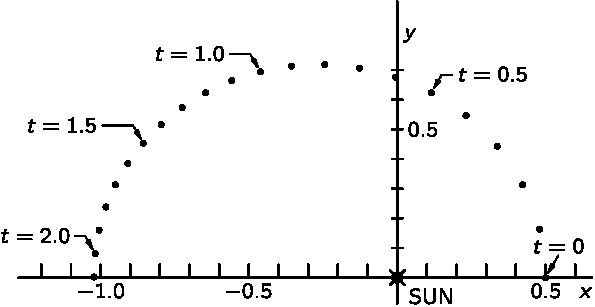
\includegraphics[width=0.7\linewidth]{fyz_fig104.pdf}
      \caption{Vypočítaný pohyb planety kolem Slunce (\cite[s.~134]{Feynman01})}
      \label{fyz:fig104}
    \end{figure}
    
    Kdyby počítači trvalo sčítání \SI{1}{\us}, násobení asi \SI{10}{\us}. Bude-li v 
    jednom výpočetním cyklu nějaké úlohy například \num{30} násobení, pak takový cyklus potrvá 
    \SI{300}{\us}. Pak můžeme za jednu sekundu provést \num{3000} výpočetních cyklů. Kdybychom 
    chtěli pracovat s přesností na jednu miliardtinu, potřebovali bychom \num{4e5} cyklů k pokrytí 
    jednoho oběhu planety kolem Slunce. To odpovídá výpočetnímu času 130 sekund, tedy asi dvěma 
    minutám. Touto metodou tedy můžeme vypočítat pohyb Jupiteru kolem Slunce s přesností na 
    jednu miliardtinu při uvážení vlivu všech ostatních planet za pouhé dvě minuty! (Ukazuje se, že 
    chyba ve výpočtech je přibližně úměrná druhé mocnině intervalů \(\varepsilon\). Zmenšíme-li 
    interval na tisícinu, zvětší se přesnost miliónkrát. Pro zajištění námi požadované přesnosti 
    musíme vzít interval \num{10000}-krát menší.)
    
    Na začátku této kapitoly jsme nevěděli ani to, jak vypočítat pohyb závaží na pružině. Nyní, 
    vyzbrojeni takovým úžasným pomocníkem, jakým jsou Newtonovy zákony, dokážeme vypočítat nejen 
    tak jednoduchý pohyb, ale pomocí počítače, který za nás provede aritmetické výpočty, i velmi 
    složité pohyby planet s takovým stupněm přesnosti, jaký požadujeme.
    
  \section{Příklady a cvičení}
      %---------------------------------------------------------------
        % !TeX spellcheck = cs_CZ
\begin{example}Výstřel z děla (ve vakuu).
  Dělová koule opouští hlaveň zadanou rychlostí. Určete:
  \begin{itemize}[noitemsep]
    \item maximální dostřel pro zadanou úsťovou rychlost,
    \item hranice oblasti, ve kterém lze zasáhnout cíl,
    \item stanovte velikost potřebného náměru děla pro zasažení libovolného cíle uvnitř ochranné paraboly.
  \end{itemize}

  {\centering
  \luafigure[1]{fyz_fig0223a.pdf}      \\
  \luafigure[0.5]{fyz_fig0223b.pdf}
  \captionsetup{type=figure}  
  \captionof{figure}{K příkladu výpočtu trajektorie projektilu. Goniometrický vzorec
           $\vert\cos\alpha\rvert=\frac{1}{\sqrt{1+\tan\alpha^2}}$ lze snadno odvodit z náčrtu
           pomocí Pythagorovy věty (Přepona pravoúhlého trojúhelníka je $\sqrt{1+\tan\alpha^2}$)}           
  \label{fyz:fig0223}
  \par}

  \textbf{Řešení:}
  Uvažujme rovinný pohyb v rovině $xz$, přičemž v záporném směru osy $z$ má pohyb zrychlení 
  velikosti $g$. Ve směru osy $z$ tedy probíhá rovnoměrně zrychlený pohyb podle rov. 
  \ref{mech:eq_const_acc}. Vztáhneme-li počáteční podmínky k okamžiku \(t = 0\), máme
  \begin{equation}\label{mech_eq_delo_vakuum_osa_z}
    z(t)=z_0+v_{0z}t-\frac{1}{2}gt^2, \qquad v_z(t)=v_{0z}-gt
  \end{equation}
  Ve směru osy \(x\) je pohyb rovnoměrný:
  \begin{equation}\label{mech_eq_delo_vakuum_osa_x}
    x(t)=x_0+v_{0x} t,\qquad v_x(t)=v_{0x}=\mathrm{konst}
  \end{equation}

  Dělová koule opouští hlaveň pod elevačním úhlem $\alpha$ za podmínek dle obr. 
  \ref{fyz:fig0223} platí $x_0=0, z_0=0, v_{0x}=v_0\cos\alpha>0, v_{0z}=v_0\sin\alpha>0$. Jde 
  tedy o skládání \emph{rovnoměrného přímočarého pohybu s rychlostí} $v_0\cos\alpha$ ve směru osy 
  \(x\) a svislého pohybu vzhůru. Získané rovnice
  \begin{equation}\label{mech:eq_delo_rce_pohybu}
    z(t)=v_{0z}t-\frac{1}{2}gt^2, \qquad x(t)=v_{0x}t
  \end{equation}
  představují \emph{parametrické rovnice trajektorie}. Vyloučíme-li z nich čas $t$, dostaneme 
  rovnici křivky v kartézských souřadnicích
  \begin{equation}\label{mech:eq_delo_vakuum_param_rce}
    z(x)=  \frac{v_{0z}}{v_{0x}}x-\frac{1}{2}\frac{g}{v_{0x}^2}x^2
        = x\tan\alpha-\frac{1}{2}\frac{g}{v_0^2\cos^2\alpha}x^2
  \end{equation}
  Nyní aplikujeme goniometrický vzorec
  \begin{equation*}
    \vert\cos\alpha\rvert = \frac{1}{\sqrt{1+\tan^2\alpha}}\Rightarrow \frac{1}{\cos^2\alpha} 
                          = 1+\tan^2\alpha
  \end{equation*}
  odvozený dle náčrtku na obrázku \ref{fyz:fig0223} a dostáváme rovnici
  \begin{equation}\label{mech_eq_example_vysledna_rce}
    z(x)=x\tan\alpha-\frac{1}{2}\frac{g}{v_0^2}(1+\tan^2\alpha)x^2
  \end{equation}
  Pohyb projektilu (dělové koule) probíhá po stejné trajektorii, jako šikmý vrh v homogenním 
  tíhovém poli ve vakuu, tedy po parabole. Snadno dostaneme \emph{souřadnice vrcholu dráhy, dálku 
  doletu a celkovou dobu letu}.

  \begin{itemize}
    \item Maximální dolet pro daný elevační úhel:
      \begin{equation}\label{mech:eq_elevacni_uhel_1}
        0=x\tan\alpha-\frac{1}{2}\frac{g}{v_0^2}(1+\tan^2\alpha)x^2
      \end{equation}
      \emph{Netriviální kořen této kvadratické rovnice je námi hledaný dolet dělové koule}
      \begin{align}  %\label{fyz:eq235}
        x_d &=\frac{2v_0^2\tan\alpha}{g(1+\tan^2\alpha)}(1+\tan^2\alpha)        \nonumber \\
            &=\frac{2v_0^2\sin\alpha\cos\alpha}{g}=\frac{v_0^2\sin{2\alpha}}{g} \label{fyz:eq235}
      \end{align}

    \item Celková doba letu:
      \begin{equation}\label{mech:eq_doba_letu}
        t_d=\frac{x_d}{v_{0x}} =\frac{2v_0^2\sin\alpha\cos\alpha}{gv_0\cos\alpha}
           =\frac{2v_0\sin\alpha}{g}
      \end{equation}

    \item Souřadnice vrcholu dráhy: \emph{získáme derivováním rov.
          \ref{mech_eq_example_vysledna_rce}}
          \begin{align}
            0   &= tan\alpha-\frac{g}{v_0^2(1+\tan^2\alpha)}x_v                         \\
            x_v &= \frac{v_0^2}{g}\frac{\tan\alpha}{1+\tan^2\alpha}=
                   \frac{v_0^2}{g}\frac{\sin\alpha}{\cos\alpha}
                   \cdot\cos^2\alpha\cdot\frac{2}{2}                                   \\
            x_v &= \frac{v_0^2\sin{2\alpha}}{2g}
           \end{align}
           \emph{Souřadnici $z_v$ dostaneme dosazením $x_v$  do rov.
           \ref{mech_eq_example_vysledna_rce}}
           \begin{align*}
             z_v &= \frac{v_0^2}{g}\frac{\tan^2\alpha}{1+\tan^2\alpha}-
                    \frac{1}{2}\frac{g}{v_0^2}(1+\tan^2\alpha)\frac{v_0^4}{g^2}
                    \frac{\tan^2\alpha}{(1+\tan^2\alpha)^2}                            \\
             z_v &= \frac{v_0^2}{g}\frac{\tan^2\alpha}{1+\tan^2\alpha}-
                    \frac{1}{2}\frac{v_0^2}{g}\frac{\tan^2\alpha}{1+\tan^2\alpha}      \\
             z_v &= \frac{v_0^2\sin^2\alpha}{2g}
      \end{align*}
      \emph{Odtud je zřejmé, že maximální délka doletu odpovídá úhlu $\frac{\pi}{4}$ a že obecně 
      daného bodu doletu lze dosáhnout pod dvěma různými úhly $\frac{\pi}{4}\pm\Delta\alpha$.}

    \item Stanovení elevačního úhlu pro zasažení zadaných souřadnic $[X_c, Z_c]$ cíle: \emph{Opět  
          vycházíme z rov. \ref{mech_eq_example_vysledna_rce}, ovšem tentokrát nejsou neznáme \(x\) a 
          $z$, ale $\alpha$: Použijeme substituci $\tan\alpha=p$ a vypočítáme kořeny této 
          kvadratické rovnice:}
          \begin{align}
            0       &= gx^2p^2-2v_0^2xp+(gx^2+2zv_0^2) \\
            p_{1,2} &= \frac{v_0^2\pm\sqrt{v_0^4-g(gx^2+2zv_0^2)}}{gx} \\
            \alpha  &= \tan^{-1}\left(\frac{v_0^2\pm\sqrt{v_0^4-g(gx^2+2zv_0^2)}}{gx}\right)
          \end{align}
          \emph{Je-li cíl zadán v polárních souřadnicích $[r,\varphi]$, lze potřebný náměr stanovit takto:}
          \begin{equation*}
            \alpha=\tan^{-1}\left(\frac{v_0^2\pm
                   \sqrt{v_0^4-g(gr^2\cos^2\varphi+2r\sin\varphi
                         v_0^2)}}{gr\cos\varphi}\right)
          \end{equation*}
          \emph{Pokud ovšem bude diskriminant menší než 0, leží cíl mimo dosah děla. Tj. neexistuje 
          takový náměr děla, kterým by bylo možné cíl zasáhnout. Je-li diskriminant roven nule, 
          jedná se o hranici, za kterou již při dané úsťové rychlosti nelze dostřelit. Body ležící 
          na této obálce tzv. ochranná parabola mohou být zasaženy pouze při jedné hodnotě 
          elevačního úhlu.}

    \item Stanovení rovnice ochranné paraboly: \emph{To provedeme tak, že položíme diskriminant 	
          rovnice pro $\tan\alpha$ roven nule a dostaneme rovnici obálky}
          \begin{equation}\label{mech:eq_ochr_parabola}
            v_0^4-g(gx^2+2zv_0^2)\Rightarrow z=-\frac{v_0^2}{2g^2}x^2+\frac{v_0^2}{2g}
          \end{equation}
  \end{itemize}

  %--------------------------Dělo---------------------------------
    \lstinputlisting[%
      style=luaMatlabStyle, 
      caption={\texttt{kinematika\_delo\_ve\_vakuu.m} pro ověření výpočtu balistické dráhy 
               projektilu.}
    ]{../src/FYZ/matlab/kinematika_delo_ve_vakuu.m}
  %---------------------------------------------------------------

  {\centering
    \captionsetup{type=figure}
    \luafigure[1]{fyz_fig0222.pdf}
    \captionof{figure}{Výpočet trajektorie projektilu ve vakuu při úsťové rychlosti $210 m/s$ 
              pomocí sw MATLAB\textsuperscript{\textregistered}.}
    \label{mech:fig_delo_matlab}
  \par}
\end{example}
      %---------------------------------------------------------------

%} %tikzset
%--------------------------------------------------------------------------------------------------- 
%==== Kapitola: Zachování hybnosti =================================================================
% !TeX spellcheck = cs_CZ
%{\tikzset{external/prefix={tikz/FYZI/}}
% \tikzset{external/figure name/.add={ch08_}{}}
%---------------------------------------------------------------------------------------------------
% file fey1ch10.tex
%---------------------------------------------------------------------------------------------------
%================= Kapitola: Zachování hybnosti ====================================================
\setchaptertoc
\chapter{Zachování hybnosti}\label{chap:fey_hybnost}

  \section{Třetí Newtonův zákon}
    Pomocí druhého Newtonova zákona, jenž dává do souvislosti zrychlení tělesa se silou na ně 
    působící, můžeme principiálně vyřešit jakýkoli problém mechaniky. Například k určení pohybu 
    několika částic můžeme použít numerickou metodu navrženou v předcházející kapitole. Existuje 
    však řada příčin dalšího studia Newtonových zákonů. Především známe zcela jednoduché případy 
    pohybu, jež je možné řešit nejen numericky, ale i přímými metodami matematické analýzy. I když 
    například víme, že zrychlení padajícího tělesa je \SI{10}{\m\per\square\s} a tento poznatek nám 
    umožňuje počítat pohyb numerickými metodami, je mnohem jednodušší a uspokojivější najít pomocí 
    matematické analýzy obecné řešení \(s = s_0 + v_0t + 5t^2\). Stejně tak v případě harmonického 
    oscilátoru jsme dokázali určit polohu numerickou metodou, ale analytickou cestou lze ukázat, že 
    obecným řešením je jednoduchá kosinová funkce času, a nemusíme proto podstoupit všechny 
    aritmetické obtíže, neboť existuje jednoduchý a přesnější způsob získání výsledku. Pohyb 
    jednoho tělesa kolem Slunce, podmiňovaný existencí gravitace, jsme v kapitole \ref{fyz:IchapIX} 
    počítali bod po bodu numerickým způsobem a získali jsme tak tvar trajektorie. Přesnou 
    analytickou metodou bychom zjistili, že tato trajektorie je dokonalou elipsou.
    
    Naneštěstí existuje jen velmi málo úloh, které lze přesně vyřešit analytickou metodou. Není-li 
    síla pružiny v případě harmonického oscilátoru úměrná výchylce, ale je složitější, musíme se 
    vrátit k numerickému řešení. Máme-li dvě tělesa pohybující se kolem Slunce, tedy celkem tři 
    tělesa, nepodaří se nám získat analytický vztah pro pohyb a takovou úlohu musíme řešit 
    numericky. Je to známý problém tří těles, s níž lidský rozum tak dlouho zápasil, až je 
    zarážející, jak dlouho trvalo, než se přišlo na to, že možnosti matematické analýzy jsou 
    omezeny a někdy je nutno použít numerické metody. Dnes se numerickými metodami řeší velké 
    množství problémů, jež není možné řešit analyticky, a problém tří těles, jenž se zdál být tak 
    těžký, se řeší zcela běžně způsobem popsaným v předcházející kapitole, tj. pomocí velkého počtu 
    aritmetických úkonů. Existují však případy, kdy analytická i numerická metoda selhávají. 
    Jednoduché úlohy umíme řešit analyticky, složitější numerickými, aritmetickými metodami, ale 
    velmi složité problémy neumíme řešit ani jedním z uvedených způsobů. Složitou úlohou je 
    například srážka dvou automobilů nebo dokonce pohyb molekul plynu. V krychlovém milimetru 
    plynu je ohromné množství částic a bylo by směšné pokoušet se o výpočty s takovým množstvím 
    proměnných (kolem \num{e17}, tj. sto miliónů miliard). Problémy, jakými jsou pohyby molekul či 
    atomů plynu nebo kousku železa, pohyby miliónů hvězd v kulových hvězdokupách a nejen dvou či 
    tří planet kolem Slunce - takové problémy nemůžeme řešit přímo a k jejich řešení musíme najít 
    jiné metody.
    
    Není-li možné zkoumat podrobnosti, zajímáme se o některé obecné vlastnosti, tj. o obecné věty 
    a principy, jež vyplývají z Newtonových zákonů. Jedním z takových principů je \textbf{zákon 
    zachování energie}, o němž se hovořilo v kapitole \ref{fyz:IchapIV}. Dalším je \textbf{zákon 
    zachování hybnosti}, jenže tématem této kapitoly. Jedním z důvodů dalšího studia mechaniky je 
    existence některých obecných vlastností pohybu, které se opakují v rozmanitých podmínkách, a 
    proto je užitečné prozkoumat tyto vlastnosti v některém speciálním případě. Budeme například 
    pozorovat srážky a zjistíme, že různé druhy srážek mají velmi mnoho společného. Uvažujeme-li 
    proudění kapaliny, není tak důležité, o kterou kapalinu jde - zákony proudění jsou podobné. 
    Další problémy, jimiž se budeme zabývat, jsou kmity a chvění a zejména zvláštní úkazy 
    mechanického vlnění - zvuk, chvění tyčí apod.
    
    Když jsme hovořili o Newtonových zákonech, zdůraznili jsme, že tyto zákony jsou jistým druhem 
    programu, který lze vyjádřit heslem „Věnujte pozornost silám“, přičemž samotný Newton nám o 
    povaze sil řekl jen dvě věci. V případě gravitace nám zanechal úplný zákon síly. V případě 
    velmi složitých sil mezi atomy Newton neznal jejich zákony, ale objevil jedno pravidlo, jednu 
    obecnou vlastnost sil, kterou vystihuje jeho třetí zákon. To je všechno, co Newton věděl o 
    povaze sil - gravitační zákon, uvedený princip a už nic víc.
    
    Jeho princip je možno vyjádřit tvrzením, že \textbf{akce je rovna reakci}. Vysvětlíme si, jak 
    chápat toto tvrzení. Předpokládejme, že máme dvě malá tělíska, např. částice, z nichž první 
    působí na druhou silou tak, že ji odtlačuje. Pak, podle třetího Newtonova zákona, druhá částice 
    působí na první stejnou silou v opačném směru; navíc, tyto síly budou působit podél stejné 
    přímky. Tato hypotéza nebo zákon vyslovený Newtonem se ukazuje být správnou, ačkoli není zcela 
    přesná (o chybách budeme hovořit později). Zatím budeme předpokládat, že akce je skutečně rovna 
    reakci. Máme-li však třetí částici, která neleží na stejné přímce jako druhé dvě, pak celková 
    síla působící na první částici není rovna celkové síle působící na druhou částici, protože na 
    obě tyto částice působí ještě částice třetí. Výsledek je takový, že celková síla působící na 
    první částici nebude ani rovna, ani opačně orientována než celková síla působící na druhou 
    částici. Celkovou sílu působící na každou z částic je však možné rozložit na části odpovídající 
    interakcím s jednotlivými částicemi. Tyto složky síly jsou pro každou dvojici vzájemně 
    působících částic stejné velikosti a opačného směru.
    
  \section{Zákon zachování hybnosti}
    Nyní si všimněme zajímavých důsledků třetího Newtonova zákona. Pro jednoduchost předpokládejme, 
    že máme jen dvě interagující částice různých hmotností, které očíslujeme jako 1 a 2. Síly 
    působící mezi nimi jsou stejné, opačně orientované a nás zajímají důsledky této skutečnosti. 
    Podle druhého Newtonova zákona je síla rovna rychlosti změny hybnosti s časem, a proto rychlost 
    změny hybnosti \(p_1\)  částice 1 je rovna záporně vzaté rychlosti změny hybnosti \(p_2\), 
    částice 2, tedy
    \begin{equation}\label{fyz:eq136}
      \der{p_1}{t} = - \der{p_2}{t}.
    \end{equation}
    
    Je-li tedy \emph{rychlost} změny vždy stejná a opačná, pak \emph{celková změna} hybnosti 
    částice 1 je stejná a opačná než celková změna hybnosti částice 2. To znamená, že při sčítání 
    hybnosti částic 1 a 2 bude rychlost změny tohoto součtu, podmíněná vzájemnými silami mezi 
    částicemi (tzv. vnitřními silami), nulová, tedy
    \begin{equation}\label{fyz:eq137}
      \der{p_1+p_2}{t} = 0.
    \end{equation}
    Je třeba zdůraznit, že v této úloze předpokládáme nepřítomnost jiných sil než vnitřních. Je-li 
    rychlost změny tohoto součtu vždy nulová, znamená to, že veličina \((p_1 + p_2)\) se nemění. 
    (Tuto veličinu píšeme i ve tvaru \(m_1v_1 + m_2v_2\) a nazýváme ji \textbf{celkovou hybností} 
    dvou částic.) Zjistili jsme tedy, že celková hybnost dvou částic se nemění, působí-li jen 
    vnitřní síly. Toto konstatování je vyjádřením zákona zachování hybnosti v uvažovaném případě. 
    Jestliže mezi dvěma částicemi působí jakkoli komplikovaná síla a změříme, nebo vypočítáme 
    \(m_1v_1 + m_2v_2\) (tedy součet hybností dvou částic) před působením a po působení této síly, 
    musíme dostat stejný výsledek, tj. \emph{celková hybnost je konstantní}.
    
    Kdybychom naše úvahy rozšířili na tři nebo více interagujících částic ve složitých podmínkách, 
    opět bychom zjistili, že při působení jen vnitřních sil zůstává celková hybnost všech částic 
    konstantní. Nárůst hybnosti jedné částice působením druhé je totiž přesně kompenzován poklesem 
    hybnosti druhé částice působením první částice. Všechny vnitřní síly budou vyvážené, a proto 
    nemohou změnit celkovou hybnost, která proto zůstává konstantní.
    
    Ještě se musíme zmínit o situaci, k níž dochází v přítomnosti sil \emph{nepocházejících} ze 
    vzájemného působení uvažovaných částic. Předpokládejme, že jsme izolovali systém interagujících 
    částic. Kdyby mezi nimi působily pouze vzájemné síly, nesměla by se jejich celková hybnost 
    měnit bez ohledu na složitost sil. Předpokládejme však, že existují síly pocházející od částic 
    nacházejících se mimo tuto izolovanou soustavu. Takovéto síly, při nichž vnější tělesa působí 
    na vnitřní, nazýváme \textbf{vnějšími silami}. Později ukážeme, že \emph{součet všech vnějších 
    sil je roven rychlosti změny celkové hybnosti všech vnitřních částic}. Je to velmi užitečná 
    věta.
    
    Zákon zachování celkové hybnosti určitého počtu interagujících částic je možné vyjádřit ve tvaru
    \begin{equation}\label{fyz:eq138}
      m_1v_1 + m_2v_2 + m_3v_3 + \ldots = \text{konst},
    \end{equation}
    jestliže nepůsobí vnější síly. Hmotnostem a rychlostem jednotlivých částic jsme přisoudili 
    indexy \(1, 2, 3, \ldots\). Pro každou z těchto částic musí být splněn druhý Newtonův zákon
    \begin{equation}\label{fyz:eq139}
      f = \der{ }{t}(mv),
    \end{equation}
    jenž platí pro každou složku síly a hybnosti v kterémkoli daném směru, a tedy \(x\)-ová složka 
    síly působící na částici je rovna rychlosti změny \(x\)-ové složky hybnosti částice
    \begin{equation}\label{fyz:eq140}
      f_x = \der{ }{t}(mv_x).
    \end{equation}
    Podobné vztahy je možno psát pro \(y\)-ovou a \(z\)-ovou složku. Rovnice (\ref{fyz:eq138}) tedy 
    ve skutečnosti představuje tři rovnice, po jedné pro každou složku.
    
    Kromě zákona zachování hybnosti existuje další zajímavý důsledek druhého Newtonova zákona. 
    Zatím ho jenom uvedeme a dokážeme ho později. Je to \emph{princip, který říká, že fyzikální 
    zákony vypadají stejně, setrváváme-li v klidu, nebo se pohybujeme rovnoměrně přímočaře}. 
    Například, jestliže si dítě hraje v letícím letadle, pozoruje, že míček skáče stejně jako na 
    zemi. I když se letadlo pohybuje velmi rychle, ale svou rychlost nemění, míček se chová stejně, 
    jako kdyby letadlo stálo na letišti. Tuto skutečnost nazýváme \textbf{principem relativity}. V 
    podobě, kterou jsme právě uvedli, nazýváme tento princip \textbf{Galileův princip relativity}, 
    abychom ho odlišili o hlubší analýzy pocházející od Einsteina, o níž budeme hovořit později.
    
    Z Newtonových zákonů jsme odvodili zákon zachování hybnosti a nyní bychom měli zkoumat, jaké 
    speciální zákony platí pro srážky. Z důvodu pestrosti, i proto, abychom ukázali jiný postup, 
    jenž se neopírá o Newtonovy zákony, budeme srážky zkoumat z úplně jiného hlediska. Naše úvahy 
    budou spočívat v uvedeném Galileově principu relativity a dopracujeme se k zákonu zachování 
    hybnosti.
    
    Začneme předpokladem, že příroda musí vypadat stejně, jestliže ji pozorujeme při přímočarém 
    rovnoměrném pohybu, nebo setrváváme-li v klidu. Dříve než budeme zkoumat procesy, v nichž se 
    dvě tělesa srážejí a spojují, nebo se při srážce od sebe odrazí, všimněme si také dvou těles, 
    jež drží pohromadě pružina nebo jiné zařízení a jež jsou náhle pružinou nebo malou explozí 
    odmrštěna. Přitom budeme uvažovat jen pohyb v jednom směru. Nejprve předpokládejme, že jde o 
    stejné, pěkně symetrické objekty, mezi nimiž došlo k malé explozi. Po explozi se bude jedno 
    těleso pohybovat vpravo rychlostí \(v\). Je rozumné předpokládat, že druhé těleso se bude 
    pohybovat vlevo rychlostí \(v\), neboť jsou-li objekty zcela stejné, není důvod dávat přednost 
    pravému nebo levému směru, a tak se bude s tělesy dít něco symetrického. To je příklad úvahy, 
    která je v mnohých úlohách velmi užitečná, ale k níž bychom nedospěli, kdybychom vycházeli jen 
    ze vzorců.
    
    Prvním výsledkem našeho experimentuje, že stejné objekty mají stejnou rychlost. Předpokládejme 
    však, že tělesa jsou vytvořena z různých materiálů, například z mědi a hliníku, ale mají stejné 
    \emph{hmotnosti}. Budeme předpokládat, že v experimentu, kdy jsou hmotnosti obou těles stejné, 
    budou jejich rychlosti stejné i tehdy, kdy tělesa stejná nejsou. Můžeme však namítnout: \uv{Je 
    možné postupovat i naopak a není třeba se opírat o takovýto předpoklad. Stačí \emph{definovat} 
    stejné hmotnosti tak, že při nich v našem experimentu dosahují tělesa stejnou rychlost.} 
    Přijmeme tento návrh a vyvoláme malou explozi mezi kouskem mědi a velmi velkým kusem hliníku, 
    který je tak těžký, že se téměř nepohne, zatímco měď odletí daleko. Hliníku je příliš mnoho, a 
    proto z něho ubereme, dokud nezůstane jen malý kousek. Když potom vyvoláme explozi, hliník 
    odletí, zatímco měď se téměř nepohne. Nyní je málo hliníku. Existuje zřejmě jakési správné 
    množství, jež lze postupně najít a při němž budou rychlosti odlétávání stejné. Podívejme se na 
    situaci jinak a prohlasme hmotnosti za stejné, jsou-li stejné rychlosti. Toto je ovšem jen 
    definice a je pozoruhodné, že fyzikální zákony můžeme transformovat do pouhých definicí. Nechť 
    je jakkoli, přece jde o následek jakýchsi fyzikálních zákonů, a jestliže přijmeme uvedenou 
    definici stejných hmotností, můžeme okamžitě najít jeden z těchto zákonů následujícím způsobem.
    
    Nechť z předcházejícího experimentu víme, že dva kousky hmoty, \(A\) a \(B\) (měď a hliník), 
    mají stejné hmotnosti. Stejným způsobem můžeme porovnat třetí těleso, například kousek zlata s 
    kouskem mědi, a ujistit se o rovnosti jejich hmotností. Provedeme-li experiment s hliníkem a 
    zlatem, nemáme žádné logické důvody k tomu, abychom \emph{jejich hmotnosti} prohlásili za 
    stejné. \emph{Experiment} nás však o tom přesvědčí. Pomocí experimentu jsme našli nový zákon. 
    Tento zákon je možné formulovat následujícím způsobem: Jestliže každá ze dvou hmotností je 
    rovna třetí hmotnosti (což se určuje rovností rychlostí v našem experimentu), pak jsou tyto dvě 
    hmotnosti stejné. (Toto tvrzení vůbec \emph{nevyplývá z} podobného tvrzení používaného jako 
    postulát v \emph{matematice}.) Na tomto příkladu je vidět, jak snadno můžeme vyslovit 
    nepodložené závěry, nejsme-li dostatečně opatrní. Tvrzení, že hmotnosti jsou stejné, jsou-li 
    stejné rychlosti, není jen definicí, neboť řekneme-li, že hmotnosti jsou stejné, znamená to, že 
    mlčky používáme matematické zákony rovnosti, což zase zpětně vede k předpovědi o experimentu.
    
    Uvažujme ještě jeden případ. Předpokládejme, že experimentem s určitou silou exploze se 
    zjistilo, že \(A\) a \(B\) jsou stejné. Ptáme se, zda při silnější explozi zůstanou rychlosti 
    stejné? Logickou cestou není možné rozhodnout tuto otázku, ale experiment ukazuje, že rychlosti 
    zůstanou stejné. Máme tedy další zákon, který říká: Zjistíme-li měřením rychlostí dvou těles, 
    že mají stejné hmotnosti, pak tato rovnost zůstane v platnosti i v měřeních při jiných 
    rychlostech. Z těchto příkladů je vidět, že to, co se zdálo být jen definicí, ve skutečnosti 
    zahrnuje určité fyzikální zákony.
    
    V dalších úvahách budeme předpokládat, že stejné hmotnosti se rozletí na opačné strany se 
    stejnými rychlostmi, jestliže mezi nimi dojde k explozi. V obrácené úloze uděláme další 
    předpoklad. Zajímáme se o to, jak se po srážce budou pohybovat dva identické objekty, které 
    letěly proti sobě stejnými rychlostmi a při srážce se pomocí nějakého lepu spojily. Opět máme 
    symetrickou situaci bez přednosti mezi pravou a levou stranou, a proto předpokládáme, že 
    utvořené těleso zůstane nehybné. Budeme předpokládat i to, že dva libovolné, stejně rychlé 
    proti sobě letící předměty stejných hmotností, i když jsou z různých materiálů, po srážce a 
    splynutí zůstanou nehybné.
        
  \section{Hybnost se zachovává}
    
    \begin{figure}[ht!]  %\ref{fyz:fig0105}
      \centering
      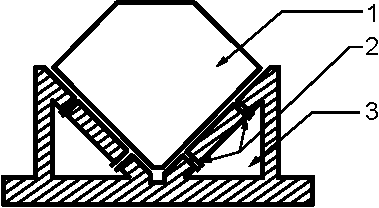
\includegraphics[width=0.5\linewidth]{fyz_fig0105.pdf}
      \caption{Příčný řez vzduchovou dráhou: 1 - klouzající předmět; 2 - malé otvory(trysky); 3 -  
               přívod stlačeného vzduchu (\cite[s.~143]{Feynman01})}
      \label{fyz:fig0105}
    \end{figure}
    Naše předpoklady o tom, že dva původně nehybné předměty stejných hmotností oddělené explozí 
    odletí na opačné strany stejnými rychlostmi a že dva předměty stejných hmotností stejně rychle 
    proti sobě letící po srážce a splynutí zůstanou nehybné, lze experimentálně prověřit. To je 
    možné provést pozoruhodným zařízením nazývaným vzduchová dráha\footnote{H. V. Neher a R. B. 
    Leighton, Amer. Jour. Of Phys. 31,255 (1963.)}. Toto zařízení nás zbavuje tření, toho tření, 
    které tak trápilo Galilea (obr. \ref{fyz:fig0105}). Galileo nemohl provádět experimenty s 
    klouzajícími předměty, neboť neklouzaly dost volně, ale uvedené zařízení nám takové experimenty 
    umožní.

    \begin{figure}[ht!]  %\ref{fyz:fig00106}
      \centering
      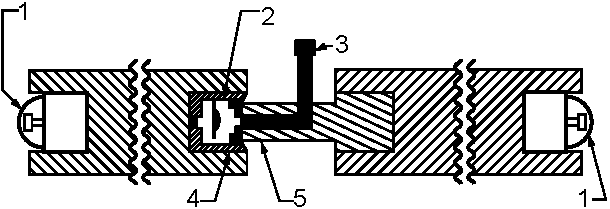
\includegraphics[width=0.7\linewidth]{fyz_fig0106.pdf}
      \caption{Podélný řez skluznými bloky spojenými výbušnou náloží: 1 - pružinový amortizátor; 2 - kapsle 
               z dětské pistole; 3 - jiskrová elektroda; 4 - válec; 5 - píst      
                \cite[s.~144]{Feynman01}}
       \label{fyz:fig0106}     
    \end{figure}

    \begin{figure}[ht!]  %\ref{fyz:fig0107}
      \centering
      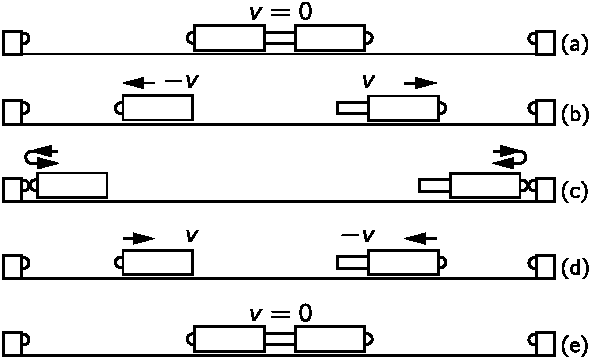
\includegraphics[width=0.7\linewidth]{fyz_fig0107.pdf}
      \caption{Schéma experimentu k demonstrace akce a reakce se stejnými hmotnostmi  
               (\cite[s.~144]{Feynman01})}
      \label{fyz:fig0107}
    \end{figure}
    Naše předměty budou bez problémů klouzat a ve shodě s Galileovou předpovědí budou mít 
    konstantní rychlost. Dosáhneme toho tak, že předměty se budou pohybovat na vzduchovém polštáři. 
    Protože tření o vzduch je velmi malé, předměty kloužou prakticky konstantní rychlostí, jestliže 
    na ně nepůsobí síla. Nejprve vezmeme dva pečlivě připravené skluzné bloky stejné tíhy a 
    hmotnosti (bloky byly jen zváženy, ale víme, že tíha je úměrná hmotnosti). Mezi tyto bloky 
    vložíme do uzavřeného válce malou výbušnou nálož (obr. \ref{fyz:fig0106}). Takto připravené 
    bloky umístíme do středu žlabu a odpálíme nálož elektrickou jiskrou. Co se stane? Jsou-li 
    rychlosti bloků po výbuchu stejné, dosáhnou bloky konce žlabu za stejnou dobu. Po dosažení 
    konců žlabu se bloky odrazí, vrátí se prakticky stejně velkými, ale opačnými rychlostmi 
    do bodu, odkud vycházely a tam se zastaví. To je zajímavý pokus a jeho výsledek je právě 
    takový, jak jsme říkali (obr. \ref{fyz:fig0107}).

    \begin{figure}[ht!]  %\ref{fyz:fig0108}
      \centering
      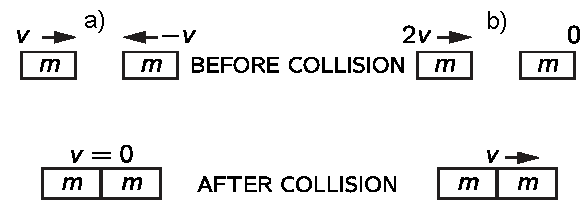
\includegraphics[width=0.7\linewidth]{fyz_fig0108.pdf}
      \caption{Dva pohledy na nepružné srážky mezi stejnými hmotnostmi: a) - pohled z těžiště, b) 
               -  pohled z jedoucího auta (rychlost auta \(= -v\))
              (\cite[s.~145]{Feynman01})}
      \label{fyz:fig0108}
    \end{figure}
    Dále bychom chtěli ukázat, co se stane ve složitější situaci. Mějme dvě stejné hmotnosti, z 
    nichž jedna se pohybuje rychlostí \(v\) a druhá stojí na místě. Co se s nimi stane, když se 
    srazí a splynou? Po ukončení srážky máme jedno těleso o hmotnosti \(2m\), jež se pohybuje 
    neznámou rychlostí. Zajímáme se o to, jakou. Abychom to zjistili, budeme předpokládat, že se 
    pohybujeme v automobilu podél jejich dráhy. Fyzikální zákony přitom zůstanou stejné, jako 
    kdybychom stáli. Naše úvahy zahájíme poznatkem, že dvě stejné hmotnosti letící proti sobě 
    stejnou rychlostí \(v\) zůstanou po srážce nehybné. Předpokládejme, že po dobu této události 
    jedeme automobilem rychlostí - \(v\). Jak potom vypadá situace? Protože se pohybujeme souběžně 
    s jednou z hmotností, jeví se nám tato tak, jakoby se nepohybovala. Druhá hmotnost, ta, jež se 
    pohybuje rychlostí \(v\) opačným směrem než my, se nám bude jevit tak, jakoby se pohybovala 
    proti nám rychlostí \(2v\) (obr. \ref{fyz:fig0108}). Po srážce se spojená hmotnost bude jevit 
    tak, jakoby procházela rychlostí \(v\), nebo, což je matematicky totéž, předmět s rychlostí 
    \(v\) po srážce a splynutí se stejným, původně nehybným předmětem, vytvoří předmět pohybující 
    se rychlostí \(v/2\). Všimněte si, že součet součinů hmotností a rychlostí před srážkou, tj. 
    \(mv + 0\), je stejný jako součet odpovídajících součinů po srážce, tj. \(2mv/2\). Taková je 
    tedy situace, když se těleso letící rychlostí \(v\) srazí s nehybným tělesem.

    Stejným způsobem je možné zjistit, co se stane, když se srazí stejné předměty letící 
    \emph{libovolnými} rychlostmi.

    \begin{figure}[ht!]  %\ref{fyz:fig0109}
      \centering
      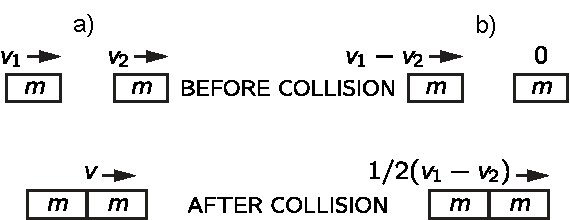
\includegraphics[width=0.7\linewidth]{fyz_fig0109.pdf}
      \caption{Dva pohledy na jinou nepružnou srážku mezi dvěma stejnými hmotnostmi: a) - pohled z 
               laboratorního systému, b)- pohled z auta
              (\cite[s.~145]{Feynman01})}
      \label{fyz:fig0109}
    \end{figure}
    Předpokládejme, že se srazí a splynou dvě stejná tělesa letící rychlostmi \(v_1\) a \(v_2\). 
    Jaká bude jejich rychlost po srážce? Pojeďme opět automobilem, a to rychlostí \(v_2\), takže 
    jedno z těles se nám bude jevit jako nehybné. Druhé se nám bude jevit tak, jakoby se pohybovalo 
    rychlostí \(v_1 - v_2\) a máme úlohu podobnou té, kterou jsme již uvažovali. Víme, že po srážce 
    se budou tělesa pohybovat rychlostí \(1/2 (v_1 - v_2)\) vzhledem k automobilu. Jaká bude 
    skutečná rychlost těles na zemi? Bude následující: \(v= 1/2(v_1-v_2) + v_2\), tedy \(1/2 (v_1 
    +v_2\) (obr. \ref{fyz:fig0108}). Všimněte si, že opět platí
     \begin{equation}\label{fyz:eq141}
      m_1v_1 + m_2v_2 = \frac{2m(v_1 + v_2)}{2}.
    \end{equation}
    
    Použitím tohoto principu můžeme analyzovat libovolnou srážku, při níž se dvě tělesa mající 
    stejné hmotnosti srazí a splynou. Ačkoli jsme ve skutečnosti pracovali jen v jednom rozměru, 
    můžeme se mnoho dozvědět o mnohem složitějších srážkách, když si představíme, že jedeme 
    automobilem v nějakém odkloněném směru. Princip zůstává stejný, jen detaily jsou složitější.

    \begin{figure}[ht!]  %\ref{fyz:fig0110}
      \centering
      \includegraphics[width=0.7\linewidth]{fyz_fig0110.pdf}
      \caption{Experiment k prověření skutečnosti, že hmotnost \(m\) narážející rychlostí \(v\) na hmotnost 
               \(m\) vytváří útvar o hmotnosti \(2m\) a rychlostí \(v/2\)
              (\cite[s.~146]{Feynman01})}
      \label{fyz:fig0110}
    \end{figure}
    Abychom experimentálně ověřili, zda předmět letící rychlostí \(v\) vytvoří po srážce se stejným 
    nehybným předmětem předmět pohybující se rychlostí \(v/2\), provedeme na vzduchové dráze 
    následující pokus. Do žlabu umístíme tři předměty se stejnou hmotností, z nichž jsou dva na 
    začátku spojeny již uvedeným explozivním válcem a třetí je sice velmi blízko, ale přece jen 
    oddělený a je na něm přilnavý nárazník, takže se přilepí k předmětu, jenž do něho narazí. V 
    prvním okamžiku po explozi máme dva předměty s hmotností \(m\), které se pohybují v opačném 
    směru stejnými rychlostmi v. V dalším okamžiku se jeden z těchto předmětů sráží s třetím 
    předmětem a vytváří předmět s hmotností \(2m\), jenž by se podle očekávání měl pohybovat 
    rychlostí \(v/2\). Jak se přesvědčíme o tom, že se pohybuje skutečně rychlostí \(v/2\)? 
    Pomůžeme si tak, že počáteční polohy předmětů ve žlabu nastavíme tak, aby vzdálenosti od konců 
    nebyly stejné, ale v poměru \(2:1\). Náš první předmět, který pokračuje v pohybu rychlostí 
    \(v\), by měl projít v dané době dvakrát takovou vzdálenost jako dva předměty, které se spojily 
    (započítáme i malou vzdálenost, již urazí druhý předmět před srážkou s třetím). Hmotnosti \(m\) 
    a \(2m\) by měly dosáhnout konce žlabu současně, a jestliže pokus uskutečníme, zjistíme, že 
    naše očekávání je správné (obr. \ref{fyz:fig0109}).

    Dále se budeme zabývat situací, kdy máme dva předměty s různými hmotnostmi. Vezměme hmotnosti 
    \(m\) a \(2m\) a nechme mezi nimi působit naši explozi. Co se pak stane? Jakou rychlostí se 
    pohybuje předmět o hmotnosti \(2m\), jestliže se předmět o hmotnosti \(m\) pohybuje v důsledku 
    exploze rychlostí \(v\)? Experiment, který jsme provedli, můžeme uskutečnit tak, že mezera mezi 
    druhým a třetím předmětem bude nulová a takový pokus nám dá stejný výsledek, tj. hmotnosti 
    \(m\) a \(2m\) dosáhnou rychlosti \(-v\) a \(v/2\). Přímá reakce mezi \(m\) a \(2m\) dává 
    stejný výsledek jako symetrická reakce mezi \(m\) a \(m\), po níž následuje srážka a spojení 
    \(m\) s třetí hmotností \(m\). Dále zjistíme, že hmotnosti \(m\) a \(2m\) se po návratu od 
    konců žlabu s téměř přesně opačnými rychlostmi zastaví, jestliže se spojí.

    Dále se můžeme ptát, co se stane, jestliže předmět o hmotnosti \(m\) letící rychlostí \(v\) 
    narazí na nehybný předmět o hmotnosti \(2m\) a spojí se s ním. Na tuto otázku můžeme odpovědět 
    velmi jednoduše, použijeme-li Galileův princip relativity a srážku, o níž jsme hovořili, 
    pozorujeme z automobilu pohybujícího se rychlostí \(-v/2\) (obr. \ref{fyz:fig0111}).

    \begin{figure}[ht!]  %\ref{fyz:fig0111}
      \centering
      \includegraphics[width=0.7\linewidth]{fyz_fig0111.pdf}
      \caption{Dva pohledy na nepružnou srážku mezi hmotnostmi \(m\) a\(2m\): a) - pohled z těžiště 
              systému, b) - pohled z auta)
              (\cite[s.~146]{Feynman01})}
      \label{fyz:fig0111}
    \end{figure}
    Při pohledu z automobilu budou rychlosti
    \begin{align*}
      v_1' &= v_1 - v_{\text{auta}} = v + \frac{v}{2} = \frac{3v}{2}   \\
      \shortintertext{a}
      v_2' &= -\frac{v}{2} - v_{\text{auta}} = - \frac{v}{2} + \frac{v}{2} = 0
    \end{align*}
    Po srážce vidíme hmotnost \(3m\) pohybovat se rychlostí \(v/2\). Takto jsme našli odpověď na 
    položenou otázku, tj. poměr rychlostí před srážkou a po srážce je \(3:1\). Sráží-li se předmět 
    o hmotnosti \(m\) s nehybným předmětem o hmotnosti \(2m\) a spojí se s ním, pak se takto 
    vytvořené těleso pohybuje rychlostí, jež je třetinou původní rychlosti. Obecné pravidlo nám 
    opět říká, že součet součinů hmotností a rychlostí zůstává stálý: \(mv + 0\) je rovno \(3m\) 
    krát \(v/3\), a tak kousek po kousku sestavujeme zákon zachování hybnosti.
    
    Zkoumali jsme srážky jednoho tělesa s dvěma tělesy. Použitím stejných argumentů můžeme 
    předpovědět výsledky srážek jednoho tělesa s třemi tělesy, dvou těles s třemi tělesy atd. Obr. 
    \ref{fyz:fig0112} znázorňuje případ srážek dvou těles s třemi tělesy a začíná situací, kdy 
    tělesa byla v klidu.
    
    \begin{figure}[ht!]  %\ref{fyz:fig0112}
      \centering
      \includegraphics[width=0.6\linewidth]{fyz_fig0112.pdf}
      \caption{Akce a reakce mezi tělesy o hmotnostech \(2m\) a \(3m\)
              (\cite[s.~147]{Feynman01})}
      \label{fyz:fig0112}
    \end{figure}
    V každém z uvedených případů zjišťujeme, že součin hmotnosti a rychlosti prvního tělesa plus 
    součin hmotnosti a rychlosti druhého tělesa je roven součinu celkové hmotnosti výsledného 
    tělesa a jeho rychlosti. Vše jsou to tedy příklady na zákon zachování hybnosti. Vycházeli jsme 
    z jednoduchých, symetrických případů a poukázali na platnost tohoto zákona v složitějších 
    případech. Tak lze postupovat v případě libovolného racionálního poměru hmotností, a protože 
    každé číslo lze s libovolnou přesností vyjádřit pomocí racionálního čísla, náš postup bude 
    možno uplatnit libovolně přesně pro jakýkoli poměr hmotností.
     
  \section{Hybnost a energie}
    Všechny předcházející příklady byly jednoduché v tom smyslu, že dvě tělesa se po srážce 
    spojila, nebo byla spojena a později oddělena explozí. Existují však případy, kdy se tělesa 
    nespojí, jako např. dvě tělesa se stejnými hmotnostmi, jež vstupují do srážky se stejnými 
    absolutními hodnotami rychlostí a po srážce se rozletí na různé strany. V kratičkém okamžiku 
    jsou v kontaktu a obě se stlačí. V okamžiku největšího stlačení mají obě dvě nulovou rychlost a 
    energie je uchována v těchto pružných tělesech tak jako ve stlačené pružině. Tato energie 
    pochází z kinetické energie, již měla tělesa před srážkou, a jež se stává nulovou, je-li 
    rychlost nulová. Ztráta kinetické energie však trvá jen okamžik. Stlačení se podobá náloži, 
    která uvolňuje energii při explozi. Ihned nastává dekomprese podobná explozi a tělesa se 
    opět rozletí. Tento případ však již známe - tělesa odletí stejnými rychlostmi. Obecně je však 
    rychlost po  odrazu menší než počáteční rychlost, neboť ne všechna energie se využije k odrazu. 
    Záleží na materiálu, jaká část energie se využije k odrazu. Je-li materiál plastický, neuvolní 
    se žádná kinetická energie, ale je-li materiál pružný, určitá část kinetické energie se uvolní. 
    Při srážce se zbytek kinetické energie přemění v tepelnou a kmitavou energii - tělesa se 
    zahřejí a kmitají. Později se i energie kmitů přemění v teplo. Srážející se tělesa je možno 
    konstruovat z velmi pružného materiálu, jakým je například ocel, a při pečlivé volbě 
    pružinových nárazníků je možné dosáhnout toho, že při srážce vzniká jen velmi málo tepla a 
    kmitů. V takovýchto podmínkách jsou rychlosti odrazu prakticky rovné počátečním rychlostem a 
    takové srážky nazýváme \textbf{pružnými}.
    
    Skutečnost, že rychlosti \emph{před} pružnou srážkou a po ní jsou stejné, není důsledkem zákona 
    zachování hybnosti, ale důsledkem zachování \emph{kinetické energie}. To, že rychlosti těles 
    odrážejících se po symetrické srážce \emph{jsou stejné}, je však důsledkem zákona zachování 
    hybnosti.
    
    Podobným způsobem můžeme analyzovat srážky mezi tělesy, která mají různé hmotnosti, počáteční 
    rychlosti i stupně pružnosti, a určit výsledné rychlosti a ztrátu kinetické energie, ale těmito 
    podrobnostmi se již nebudeme zabývat.
    
    Pružné srážky jsou zvlášť zajímavé v systémech, které nemají vnitřní „kolečka, ozubená kola 
    nebo jiné části“. V takových systémech nemá energie při srážkách kam unikat, neboť odrážející 
    se objekty se nacházejí ve stejných podmínkách jako před srážkou. Proto se mezi elementárními 
    objekty uskutečňují pružné nebo téměř pružné srážky. Například srážky mezi atomy nebo 
    molekulami plynu jsou považovány za dokonale pružné. Ačkoli tu jde o výbornou aproximaci, ani v 
    takovémto případě nejsou srážky \emph{dokonale} pružné - jinak si nemůžeme vysvětit, odkud bere 
    plyn energii na světelné a tepelné záření. Občas se při srážkách v plynu emituje 
    nízkoenergetické infračervené záření. Jeho výskyt je však velmi ojedinělý a emitovaná energie 
    je velmi malá. Srážky molekul v plynech je proto většinou možno považovat za dokonale pružné.
    
    Všimněme si zajímavého příkladu \emph{pružných} srážek mezi dvěma tělesy se \emph{stejnými 
    hmotnostmi}. Přibližují-li se takováto tělesa k sobě stejně velkými rychlostmi, pak se z důvodů 
    symetrie budou od sebe vzdalovat stejnými rychlostmi. Podívejme se však na tento proces v jiné 
    situaci, kdy jedno z nich se pohybuje rychlostí \(v\) a druhé je v klidu. Co se stane? S něčím 
    podobným jsme se již setkali. Symetrickou srážku budeme pozorovat z auta pohybujícího se 
    souběžně s jedním z těles a zjistíme, že pohybující se těleso při pružné srážce s nehybným 
    tělesem stejné hmotnosti zastaví, a to, které bylo v klidu, se bude pohybovat stejnou rychlostí 
    jako první těleso. Tělesa si prostě vymění rychlosti\footnote{Tento výsledek poprvé publikoval 
    český fyzik Jan Marek Marci v roce 1639.}. Takové chování lze snadno ověřit vhodným srážkovým 
    zařízením. Obecně, pohybují-li se obě tělesa proti sobě různými rychlostmi, prostě si při 
    srážce rychlosti vymění. Jiným příkladem téměř pružných interakcí je magnetizmus. Umístíme-li 
    dvojici podkovovitých magnetů na naše kluzné bloky tak, že se vzájemně odpuzují, pak při 
    opatrném posunutí jednoho směrem k druhému dojde k odtlačení druhého magnetu, první magnet se 
    úplně zastaví a druhý se pak bude bez tření pohybovat.
    
    Zákon zachování hybnosti je velmi užitečný a umožňuje nám vyřešit mnoho problémů bez jejich 
    podrobného zkoumání. Neznali jsme detailně pohyb plynu při výbuchu nálože, a přece jsme 
    například dokázali předpovědět rychlosti, s jakými se tělesa odrazí. Dalším zajímavým příkladem 
    je raketový motor. Raketa s velkou hmotností \(M\) vymršťuje malé množství plynů hmotnosti 
    \(m\), ale obrovskou rychlostí \(V\) vzhledem k samotné raketě. Původně nehybná raketa se proto 
    začne pohybovat malou rychlostí \(v\). Pomocí zákona zachování hybnosti můžeme tuto rychlost 
    vypočítat, a tak dostaneme
    \begin{equation}\label{fyz:eq142}
      v = \frac{m}{M}\cdot V.
    \end{equation}
    Pokud je plyn vymršťován, raketa nabírá rychlost. Raketový pohon je v podstatě totéž, co zpětný 
    náraz pušky; nepotřebuje vzduch k tomu, aby se od něho odrážel.
    
  \section{Relativistická hybnost}
    Není to tak dávno, co zákon zachování hybnosti postihly určité změny. Samotný zákon sice stále 
    platí, ale změny nastaly v definici. V \emph{teorii relativity} se ukazuje, že zákon zachování 
    hybnosti platí. Částice mají hmotnost, a hybnost je definována opět jako součin hmotnosti a 
    rychlosti, tj. \(mv\), jenže hmotnost se v závislosti na rychlosti mění, a proto se bude měnit 
    i hybnost. Změna hmotnosti podléhá zákonu
    \begin{equation}\label{fyz:eq143}
      m = \dfrac{m_0}{\sqrt{1 - \dfrac{v^2}{c^2}}}.
    \end{equation}
    kde \(m_0\) je hmotnost tělesa v \emph{klidu}, \(c\) je rychlost světla. Z tohoto vztahuje 
    zřejmé, že \(m\) se jen nepatrně liší od \(m_0\), pokud v není velmi velká, a tak pro běžné 
    rychlosti je možné vyjádřit hybnost starým vztahem.
    
    Složky hybností jedné částice lze zapsat ve tvaru
    \begin{equation}\label{fyz:eq144}
      p_x = \dfrac{m_0v_x}{\sqrt{1 - \dfrac{v^2}{c^2}}}, \quad
      p_y = \dfrac{m_0v_y}{\sqrt{1 - \dfrac{v^2}{c^2}}}, \quad
      p_z = \dfrac{m_0v_z}{\sqrt{1 - \dfrac{v^2}{c^2}}},
    \end{equation}
    přičemž \(v^2 = v_x^2 + v_y^2 + v_z^2\). Sečteme-li \(x\)-ové složky všech interagujících 
    částic nejprve před srážkou a pak po srážce, zjistíme, že tyto součty jsou stejné, tj. hybnost 
    ve směru osy \(x\) se zachovává. Totéž platí v libovolném směru.
    
    V kapitole \ref{fyz:IchapIV} jsme viděli, že zákon zachování energie neplatí, nepřipustíme-li 
    existenci různých forem energie: elektrické, mechanické, tepelné, zářivé apod. V některých z 
    těchto případů (např. u tepelné energie) je možno říci, že energie se vyskytuje v „skryté“ 
    formě. Tento příklad nás může inspirovat k otázce: „Existují i skryté formy hybnosti - 
    například tepelná hybnost?“  Odpověď na tuto otázku je, že hybnost se dá velmi obtížně skrýt, a 
    to z následujících důvodů.
    
    Součet druhých mocnin rychlostí neuspořádaně se pohybujících atomů tělesa představuje míru 
    tepelné energie. Jako výsledek dostaneme kladnou veličinu bez směrového charakteru. Teplo 
    existuje bez ohledu na to, zda se těleso jako celek pohybuje, nebo zda je nehybné, a zachování 
    energie v podobě tepla není přímo zřejmé. Dostaneme-li však při sčítání \emph{rychlostí}, které 
    mají směr, výsledek různý od nuly, znamená to, že existuje pohyb samotného tělesa v jistém 
    směru, a ten již můžeme viditelně pozorovat. Neexistuje tedy náhodná, uvnitř utajená hybnost; 
    těleso má nenulovou hybnost jen tehdy, když se pohybuje jako celek. Proto lze hybnost jako 
    mechanickou veličinu těžko skrýt. Hybnost je však přece jenom \emph{možné} skrýt - např. v 
    elektromagnetickém poli. To je další zvláštnost teorie relativity.
    
    Newton předpokládal, že vzájemné působení se bez ohledu na vzdálenost uskutečňuje okamžitě. 
    Tento předpoklad se ukázal být nesprávným. Uvažujeme-li například i elektrické síly a v určitém 
    místě uvedeme do pohybu elektrický náboj, pak se jeho vliv na jiný náboj v jiném místě 
    neprojeví okamžitě - existuje malé zpoždění. V takovéto situaci i při rovnosti sil akce a 
    reakce se hybnosti nebudou kompenzovat; bude existovat krátký časový interval, v jehož průběhu 
    nastanou problémy. V této době pocítí první náboj určitou sílu reakce a získá určitou hybnost, 
    zatímco druhý náboj ještě nepocítil nic a jeho hybnost se nezměnila. Vzájemné působení 
    potřebuje k překlenutí vzdálenosti určitou dobu, takovou, jako kdyby se šířilo rychlostí 
    \SI{300000}{\km\per\s}. V průběhu takovéhoto kraťoučkého intervalu se hybnost částic 
    nezachovává. Pocítí-li však druhý náboj působení prvního náboje a vše se ustálí, zákon 
    zachování hybnosti bude opět platit; nezachovává se tedy jen po krátkou dobu. Záhadný je tedy 
    jen ten krátký časový interval. Situaci si představujeme tak, že v tomto intervalu existuje i 
    jiná hybnost, než je hybnost částic \(mv\). Jde o hybnost elektromagnetického pole. Přidáme-li 
    tuto hybnost pole k hybnosti částic, pak se hybnost zachovává v kterémkoli okamžiku. To, že 
    elektromagnetické pole může mít hybnost a energii, ho činí skutečné reálným, a tak původní 
    myšlenku o existenci sil mezi částicemi je třeba pozměnit v tom smyslu, že částice vytváří pole 
    a pole působí na jinou částici. Samotné pole má dobře známé vlastnosti jako jsou energie a 
    hybnost, vlastnosti, které mají částice. Jako další příklad si všimněme elektromagnetického 
    pole, v němž existují vlny nazývané světlem. Ukazuje se, že světlo má i hybnost, a proto při 
    dopadu na předmět přináší i určité množství hybnost. To je ale rovnocenné působení síly, neboť 
    získává-li osvětlený předmět určité množství hybností za sekundu, jeho hybnost se mění a 
    situace je stejná, jako kdyby na něj působila síla. Při dopadu na předmět vyvolává světlo tlak. 
    Tento tlak je velmi malý, ale dostatečně citlivými zařízeními ho můžeme změřit.
   
    V kvantové mechanice se ukazuje, že hybnost je něco jiného - už to není \(mv\). Je těžké přesně 
    definovat, co je to rychlost částice, ale hybnost přece existuje. V kvantové mechanice je 
    rozdíl v tom, že když se částice chovají jako částice, je hybnost \(mv\), ale když se chovají 
    jako vlny, měří se hybnost počtem vln najeden metr: Čím větší je počet vln, tím větší je 
    hybnost. Bez ohledu na tyto rozdíly platí zákon zachování hybnosti i v kvantové mechanice. 
    Ačkoli zákon \(f= ma\) v kvantové mechanice neplatí a Newtonovo odvození zákona zachování 
    hybností je nesprávné, přece jen v kvantové mechanice samotný zákon zachování hybnosti platí!
    
    
  \section{Příklady a cvičení}
  
%} %tikzset
%--------------------------------------------------------------------------------------------------- 
%==== Kapitola: Vektory ============================================================================
% !TeX program = lualatex
% !TeX root = luaking.tex
% !TeX encoding = UTF-8
% !TeX spellcheck = cs_CZ
%---------------------------------------------------------------------------------------------------
% file fey1ch11.tex
%---------------------------------------------------------------------------------------------------
%================= Kapitola: Vektory ===============================================================
\setchaptertoc
\chapter{Vektory}\label{fyz:IchapXI}
  \section{Symetrie ve fyzice}
    V této kapitole zavedeme pojem, jenž je ve fyzice známý jako \emph{symetrie fyzikálních 
    zákonů}. Slovo \uv{symetrie} tu používáme ve zvláštním smyslu, a proto bude třeba ho definovat. 
    Je-li nějaká věc symetrická - jak to můžeme definovat? Říkáme-li, že obraz je symetrický, 
    rozumíme tím, že jeho jedna strana je nějak stejná jako druhá. Profesor Hermann Weyl definoval 
    symetrii takto: Předmět je symetrický, můžeme-li ho podrobit určité operaci a po ní bude stejný 
    jako původně. Například, podíváme-li se na vázu, jež má pravo-levou symetrii, pak otočením o 
    \SI{180}{\degree} kolem vertikální osy bude vypadat opět stejně. Přijmeme Weylovu obecnější 
    definici symetrie a na jejím základě budeme hovořit o symetrii fyzikálních zákonů.
    
    Předpokládejme, že na určitém místě jsme postavili složité zařízení s množstvím interakcí, se
    srážejícími se kuličkami, mezi nimiž působí síly atd. Dále předpokládejme, že na jiném místě
    jsme vybudovali přesně stejné zařízení, jehož všechny části jsou shodné se stejnými rozměry a
    stejnou orientací - vše je stejné, jen je to posunuto o určitou vzdálenost. Ptáme se, zda se
    budou tato zařízení chovat úplně stejně, jestliže je, uvedeme do činnost za stejných počátečních
    podmínek? Budou všechny pohyby paralelní? Odpověď může být samozřejmě záporná, neboť místo pro
    druhé zařízení může být nevhodně zvoleno. Zvolíme-li toto místo někde u stěny, druhé zařízení
    nebude moci vůbec pracovat, neboť stěna při některých pohybech překáží.
    
    Naše fyzikální úvahy vyžadují určitý zdravý smysl při jejich aplikaci, vždyť to nejsou čistě 
    matematické nebo abstraktní myšlenky. Musíme vědět, co to znamená, když hovoříme, že při 
    přesunu zařízení na nové místo pozorujeme stejné jevy. Znamená to, že přemisťujeme vše, co může 
    mít na pohyb vliv. Nepozorujeme-li stejný jev, pak jsme něco důležitého nepřemístili a budeme 
    muset zjistit, co to je. Nezjistíme-li to nikdy, pak můžeme prohlásit, že fyzikální zákony 
    nemají takovou symetrii. Mají-li však fyzikální zákony takovou symetrii, pak příčinu neshody 
    můžeme najít - a my doufáme, že ji najdeme. Například, jestliže se pozorně rozhlédneme, můžeme 
    zjistit, že stěna působí na naše zařízení. Základní otázkou je, zda při dostatečně dobře 
    definovaných poměrech, při započtení všech podstatných sil a přesunu všech důležitých částí na 
    jiné místo budou zákony stejné. Bude zařízení pracovat stejně?
    
    Je jasné, že chceme přesunout celé zařízení a všechny \emph{podstatné} vlivy, ale ne 
    \emph{všechno} na světě - planety, hvězdy a všechno ostatní. Kdybychom totiž přesunuli všechno, 
    měli bychom stejný jev jako původně z toho prostého důvodu, že bychom se ocitli na stejném 
    místě. \emph{Všechno} tedy nemůžeme přesunout. V praxi se ukazuje, že při rozumném výběru 
    přesouvaných věcí bude zařízení pracovat stejně. Jinými slovy, nenarazíme-li na stěnu, 
    budeme-li znát původ vnějších sil a zabezpečíme i jejich přesun, pak bude zařízení pracovat na 
    obou místech stejně.
    
  \section{Translace}\label{fyz:IchapXIsecI}
    V našich úvahách se omezíme na mechaniku, o níž toho víme již dost. V předcházející kapitole
    jsme poznali, že zákony mechaniky je možné shrnout do tří rovnic pro každou částici
    \begin{equation}\label{fyz:eq145}
      m\dder{x}{t} = F_x, \;
      m\dder{y}{t} = F_y, \;
      m\dder{z}{t} = F_z.
    \end{equation}

    \begin{figure}[ht!]  %\ref{fyz:fig0113}
      \centering
      \includegraphics[width=0.8\linewidth]{fyz_fig0113.pdf}
      \caption{Dvě paralelní soustavy souřadnic (\cite[s.~154]{Feynman01})}
      \label{fyz:fig0113}
    \end{figure}
    To znamená, že existuje způsob měření vzdáleností \(x, y, z\) na třech navzájem kolmých osách i
    sil podél těchto směrů, a při takovém měření jsou rovnice (\ref{fyz:eq145}) pravdivé. Měření
    musí být realizována od nějakého počátku a my se ptáme, \emph{kde má být tento počátek}. Newton
    by nám řekl jen tolik, že takové místo, ze kterého je možné začít měřit, existuje - snad je to
    střed vesmíru - a při takovém měření jsou uvedené zákony správné. Snadno však nahlédneme, že
    takový střed nikdy nenajdeme, protože nic by se nezměnilo, kdybychom si zvolili jiný počátek.
    Předpokládejme, že existují dva lidé - Petr, který si zvolil počátek na jednom místě, a Pavel,
    který má paralelní soustavu s počátkem na jiném místě (obr. \ref{fyz:fig0113}). Při měření polohy
    bodu v prostoru zjistí Petr, že má souřadnice \(x\), \(y\) a \(z\) (obvykle budeme vynechávat
    \(z\), abychom se vyhnuli komplikacím při kreslení obrázků). Když měří polohu stejného bodu
    Pavel, zjistí, že má hodnotu \(x\) (pro rozlišení ji budeme označovat \(x'\)) a obecně jinou
    hodnotu \(y\), ačkoli v našem příkladu jsou tyto hodnoty číselně stejné. Máme tedy
    \begin{equation}\label{fyz:eq146}
      x' = x - a, \quad y' = y, \quad z' = z.
    \end{equation}
    Aby byla naše analýza úplná, musíme vědět, jaké síly naměří Pavel. Síla působí podél nějaké 
    přímky a silou ve směru osy \(x\) rozumíme tu část z celkové síly, jež působí podél osy \(x\) a 
    získáme ji tak, že násobíme velikost síly kosinem úhlu, který svírá s osou \(x\). Tak 
    zjišťujeme, že Pavel bude mít stejné průměty jako Petr a máme proto soustavu rovnic
    \begin{equation}\label{fyz:eq147}
      F_{x'} = F_x, \quad F_{y'} = F_y, \quad F_{z'} = F_z.
    \end{equation}
    Tyto rovnice představují vztahy mezi veličinami, které vidí Petr a Pavel.
    
    Položme si otázku: Zná-li Petr Newtonovy zákony a snaží-li se Pavel objevit zákony pohybu, 
    budou tyto jeho zákony shodné s Newtonovými? Projeví se nějak změněná volba počátku? Jinak 
    řečeno, jsou-li rovnice (\ref{fyz:eq145}) správné a rovnice (\ref{fyz:eq146}) a 
    (\ref{fyz:eq147}) představují vztahy mezi měřenými veličinami, platí, nebo neplatí následující 
    vztahy?
    \begin{flalign}\label{fyz:eq148}
      m\dder{x'}{t} = F_{x'}, \;
      m\dder{y'}{t} = F_{y'}, \;
      m\dder{z'}{t} = F_{z'}. &&
    \end{flalign}
    Abychom tyto rovnice prověřili, derivujeme dvakrát vztah pro \(x'\). Nejprve dostaneme
    \begin{equation*}
      \der{x'}{t} =\der{ }{t}(x-a) = \der{x}{t} - \der{a}{t}.
    \end{equation*}
    Budeme předpokládat, že Pavlův počátek je pevný, nepohybuje se vzhledem k Petrovu počátku. 
    Proto je \(a\) konstanta a \(da/dt=0\), takže máme
    \begin{equation*}
      \der{x'}{t} = \der{x}{t} \quad\text{a dále}\quad \dder{x'}{t} = \dder{x}{t}.
    \end{equation*}
    Protože předpokládáme, že hmotnosti měřené Petrem a Pavlem jsou stejné, získá rovnice 
    (\ref{fyz:eq148}) pro osu \(x\) tvar
    \begin{equation*}
      m\dder{x}{t} = F_{x'}.
    \end{equation*}
    Součin hmotnosti a zrychlení je tedy u obou pozorovatelů stejný. Získali jsme i vztah pro 
    \(F_{x'}\), neboť po dosazení do rovnice (\ref{fyz:eq145}) zjistíme, že
    \begin{equation*}
      F_{x'} = F_{x}.
    \end{equation*}
    
    Zákony, jež odvodí Pavel, vypadají tedy stejně jako Petrovy. I pro něho platí Newtonovy zákony, 
    i když s jinými souřadnicemi. To znamená, že neexistuje střed vesmíru a pohybové zákony budou 
    stejné bez ohledu na místo, z něhož pozorujeme.
    
    Platí i následující tvrzení: Je-li na určitém místě zařízení obsahující jistý mechanizmus, pak
    stejné zařízení bude na jiném místě pracovat stejné. Proč? Protože zařízení analyzované Pavlem
    vyhovuje stejným rovnicím jako zařízení analyzované Petrem. Protože jsou rovnice stejné, budou
    stejné i jevy. Důkaz toho, že zařízení se na novém místě chová stejně jako na původním, je
    stejný jako důkaz toho, že rovnice přenesené na jiné místo prostoru se reprodukují. Můžeme tedy
    prohlásit, že \textbf{fyzikální zákony jsou symetrické vzhledem k translaci v prostoru},
    symetrické v tom smyslu, že zákony se nemění při translaci soustavy souřadnic. Že je to pravda,
    je celkem zřejmé intuitivně, ale je zajímavé a zábavné se zabývat matematickou stránkou této
    záležitosti. K problému se ještě vrátíme v kapitole \ref{fyz:IchapXVsecIII}, ve které se budeme
    zabývat \textbf{principem relativity}. 
    
  \section{Rotace}\label{fyz:IchapXIsecII}
    Předcházející část byla věnována první z řady stále komplikovanějších tvrzení týkajících se 
    symetrie fyzikálních zákonů. Další tvrzení praví, že nezáleží na tom, v jakém \emph{směru} 
    zvolíme souřadnicové osy. Jinými slovy, postavíme-li někde jedno zařízení a v sousedství 
    stejné zařízení, ale pootočíme ho o určitý úhel vzhledem k prvnímu zařízení, ptáme se, zda 
    budou obě dvě zařízení pracovat stejně. Určitě nebudou, jsou-li takovým zařízením, například, 
    dědečkovy kyvadlové hodiny! Je-li kyvadlo ve svislé poloze, hodiny spolehlivě pracují, ale 
    nakloníme-li hodiny, kyvadlo narazí na stěnu pouzdra a hodiny se zastaví. V případě kyvadlových 
    hodin je naše tvrzení nesprávné, pokud do zařízení nezahrneme i Zemi, jež působí na pohyb 
    kyvadla. Věříme-li, že fyzikální zákony jsou symetrické vzhledem k rotaci, musíme připustit, že 
    na chod kyvadlových hodin má vliv i něco jiného než kyvadlový stroj, něco mimo hodiny, a my to 
    musíme najít. Ještě můžeme předpovědět, že kyvadlové hodiny nebudou pracovat stejně, budou-li 
    umístěny na různých místech, vzhledem k tomu záhadnému zdroji asymetrie, jímž je snad Země. 
    Skutečně, kyvadlové hodiny umístěné například na umělé družici Země, nepůjdou, neboť tam není 
    efektivní síla a na Marsu by zase měly jinou rychlost. Kyvadlové hodiny \emph{představují} něco 
    více než jednoduchý mechanizmus v jejich vnitřku, zahrnují i něco, co je mimo ně. Známe-li 
    tento faktor, pochopíme, že bychom museli společně s celým zařízením pootočit i Zemi. Nemusíme 
    si však dělat starosti s pootočením Země, stačí chvíli počkat a Země se pootočí sama; pak 
    půjdou kyvadlové hodiny v nové poloze stejně jako předtím. Zatímco rotujeme v prostoru, mění se 
    absolutně i naše úhly; tyto změny nás však příliš neznepokojují, neboť v nové poloze se cítíme 
    stejně dobře jako ve staré. Taková situace nás může zmýlit. V nové pootočené poloze jsou sice 
    zákony stejné jako před pootočením, \emph{není však pravda}, že by \emph{po dobu otáčení} věci 
    podléhaly stejným zákonům, jako když se neotáčejí. Uskutečníme-li dostatečně přesné 
    experimenty, můžeme zjistit, zda Země \emph{rotuje}, ale nemůžeme zjistit, zda Země 
    \emph{rotovala}. Jinými slovy, takto nemůžeme zjistit její orientaci, ale jen skutečnost, že 
    tato orientace se mění.

    \begin{figure}[ht!]  %\ref{fyz:fig0114}
      \centering
      \includegraphics[width=0.8\linewidth]{fyz_fig0114.pdf}
      \caption{Dvě soustavy souřadnic s různou úhlovou orientací
              (\cite[s.~156]{Feynman01})}
      \label{fyz:fig0114}
    \end{figure}
    Nyní uvažujme vliv úhlové orientace na fyzikální zákony. Zjistíme, jak to bude nyní s Petrem a 
    Pavlem. Abychom vyloučili zbytečné komplikace, budeme předpokládat, že Petr i Pavel vycházejí 
    ze společného počátku (již jsme ukázali, že jejich souřadnicové systémy se mohou translací 
    přesunout na jiné místo). Předpokládejme, že Pavlovy osy se pootočily vzhledem k Petrovým osám 
    o úhel \(\vartheta\). Omezíme-li se na dvojrozměrný prostor, můžeme dvě takové soustavy 
    souřadnic znázornit jako na obr. \ref{fyz:fig0114}. Uvažujme nějaký bod \(P\), jež má v Petrově 
    soustavě souřadnice \((x, y)\) a v Pavlově soustavě souřadnice \((x' y')\). Podobně jako v 
    předcházejícím případě, začneme tím, že vyjádříme souřadnice \(x', y'\) pomocí \(x, y\) a 
    \(\vartheta\). Abychom to mohli realizovat, vedeme nejprve kolmice z \(P\) ke všem čtyřem osám 
    a nakreslíme \(AB\) kolmo k \(PQ\). Z obrázku je vidět, že \(x'\) lze vyjádřit jako součet dvou 
    úseček podél osy \(x'\) a \(y'\) zase jako rozdíl dvou úseček podél \(AB\). Délky těchto úseček 
    jsou vyjádřeny pomocí \(x, y\) a rovnicích (\ref{fyz:eq149}), k nimž připojíme rovnici pro 
    třetí rozměr

    \begin{subequations}\label{fyz:eq149}
      \begin{align}
        x' &= x\cos\vartheta + y\cos\vartheta, \label{fyz:eq149a} \\
        y' &= y\cos\vartheta - x\sin\vartheta, \label{fyz:eq149b} \\
        z' &= z.
      \end{align}
    \end{subequations}

    Dalším krokem je analýza vztahů mezi silami naměřenými dvěma pozorovateli, kterou provedeme 
    podobně jako v předchozím případě. Předpokládejme, že síla \(F\), kterou jsme již analyzovali, 
    má složky \(F_x\) a \(F_y\) (při Petrově pozorování) a působí na částici o hmotnosti \(m\), 
    nacházející se v bodě \(P\) (obr. \ref{fyz:fig0114}). Pro zjednodušení posuňme obě souřadnicové 
    soustavy tak, že počátek bude v bodě \(P\) (obr. \ref{fyz:fig0115}).
    
    \begin{figure}[ht!]  %\ref{fyz:fig0115}
      \centering
      \includegraphics[width=0.8\linewidth]{fyz_fig0115.pdf}
      \caption{Složky síly ve dvou soustavách
              (\cite[s.~157]{Feynman01})}
      \label{fyz:fig0115}
    \end{figure}

    Pavel pozoruje podél svých os složky síly \(F_{x'}\), a \(F_{y'}\). \(F_{x}\) má složky ve 
    směrech \(x'\) a \(y'\) a právě tak i \(F_y\). Abychom vyjádřili \(F_{x'}\), pomocí \(F_x\) a 
    \(F_y\), sčítáme složky těchto sil podél osy \(x'\). Podobně můžeme vyjádřit \(F_{y'}\), pomocí 
    \(F_x\) a \(F_y\). Tak dostaneme
    \begin{subequations}\label{fyz:eq155}
      \begin{align}
        F_{x'} &= F_x\cos\vartheta + F_y\sin\vartheta, \label{fyz:eq155a}\\
        F_{y'} &= F_y\cos\vartheta - F_x\sin\vartheta, \label{fyz:eq155b}\\
        F_{z'} &= F_z.                                 \label{fyz:eq155c}
      \end{align}
    \end{subequations}
    Je třeba si všimnout, že vztahy (\ref{fyz:eq149}) a (\ref{fyz:eq155}) pro souřadnice \(P\) a 
    složky \(F\) \emph{mají shodný tvar}. Tato náhodná shoda má velký význam.
    
    Tak jako v přecházejícím případě, předpokládejme, že v Petrově soustavě platí Newtonovy zákony, 
    jež jsou vyjádřeny rovnicemi (\ref{fyz:eq145}). Opět se ptáme, zda Pavel může použít Newtonovy 
    zákony - zda dostane správné výsledky ve své soustavě s pootočenými osami? Jinými slovy, 
    předpokládáme-li, že rovnice (\ref{fyz:eq149}) a (\ref{fyz:eq155}) vyjadřují souvislost mezi 
    měřeními, budou, nebo nebudou správné následující vztahy?
    
    \begin{subequations}\label{fyz:eq156}
      \begin{align}
        m\dder{x'}{t} &= F_{x}, \label{fyz:eq156a}  \\
        m\dder{y'}{t} &= F_{y}, \label{fyz:eq156b}  \\
        m\dder{z'}{t} &= F_{z}. \label{fyz:eq156c}
      \end{align}
    \end{subequations}
    
    Zkoušku správnosti provedeme tak, že nezávisle vypočteme jejich levé i pravé strany a porovnáme 
    výsledky. Výpočet levých stran provádíme tak, že rovnice (\ref{fyz:eq149}) násobíme \(m\) a za 
    předpokladu, že úhel \(\vartheta\) je konstantní, dvakrát derivujeme podle času. Takovýmto 
    způsobem dostaneme
    \begin{subequations}
      \label{fyz:eq157}
      \begin{align}
        m\dder{x'}{t} &= 
          m\dder{x}{t}\cos\vartheta + m\dder{y}{t}\sin\vartheta, \label{fyz:eq157a}\\
        m\dder{y'}{t} &= 
          m\dder{y}{t}\cos\vartheta - m\dder{x}{t}\sin\vartheta, \label{fyz:eq157b}\\
        m\dder{z'}{t} &= 
          m\dder{z}{t}.                                          \label{fyz:eq157c}
      \end{align}
    \end{subequations}
    Pravé strany rovnic (\ref{fyz:eq156}) vypočteme tak, že rovnice (\ref{fyz:eq148}) dosadíme do 
    rovnic (\ref{fyz:eq155}). Tak dostaneme
    \begin{subequations}
      \label{fyz:eq158}
      \begin{align}
        F_{x'} &= m\dder{x}{t}\cos\vartheta + m\dder{y}{t}\sin\vartheta, \label{fyz:eq158a}\\
        F_{y'} &= m\dder{y}{t}\cos\vartheta - m\dder{x}{t}\sin\vartheta, \label{fyz:eq158b}\\
        F_{z'} &= m\dder{z}{t}.                                          \label{fyz:eq158c}
      \end{align}
    \end{subequations}
    
    Vida! Pravé strany rovnic (\ref{fyz:eq157}) a (\ref{fyz:eq158}) jsou shodné, a proto jsou-li
    Newtonovy zákony správné v jedné soustavě souřadnic, jsou správné i v druhé souřadnicové
    soustavě. Tento výsledek, platný pro translaci i rotaci os, má jisté důsledky. Především, nikdo
    nemůže tvrdit, že jím zvolené souřadnicové osy jsou jediné, ačkoli mohou být \emph{nejvhodnější}
    pro určitý problém. Například, je vhodné zvolit souřadnicovou soustavu tak, aby gravitační síla
    působila ve směru jedné osy, ale není to fyzikálně nezbytné. Dalším důsledkem je skutečnost, že
    každé zařízení, zcela soběstačné v tom smyslu, že obsahuje vše, co na něho silově působí, bude
    pracovat stejně při jakémkoli pootočení.
    
  \section{Vektory}\label{fyz:IchapXIsecIII}
    Nejen Newtonovy, ale pokud dnes víme i ostatní zákony fyziky mají dvě vlastnosti, jež nazýváme 
    \textbf{invariancí} (nebo symetrií) vzhledem k translaci a rotaci souřadnicových os. Tyto 
    vlastnosti jsou tak důležité, že k jejich využití při studiu fyzikálních zákonů vznikla 
    speciální matematická metoda.
    
    Předchozí analýza vyžadovala dosti pracné matematické výpočty. Aby při řešení těchto otázek 
    bylo možno omezit detailní výpočty na minimum, byl vytvořen velmi účinný matematický aparát. 
    Nazývá se \textbf{vektorová analýza} a je vlastně obsahem této kapitoly; přesně vzato však naše 
    kapitola pojednává o symetrii fyzikálních zákonů. Předcházející metody nám umožňovaly získat 
    všechny požadované výsledky, ale v praxi bychom je chtěli získat jednodušeji a rychleji, a 
    proto zavedeme vektorovou metodu.
    
    Začneme tím, že si všimneme některých rysů dvou druhů veličin, jež jsou ve fyzice důležité. (Ve 
    skutečnosti je takových druhů více, ale začneme jen se dvěma.) První druh veličin je takový, 
    jako počet brambor v pytli a tyto veličiny nazýváme obyčejnými nebo nesměřovanými čísly neboli 
    \textbf{skaláry}. Takovou veličinou je například teplota. Jiné ve fyzice důležité veličiny mají 
    směr. Je to například rychlost: Nestačí znát jen velikost rychlosti přemisťování tělesa, ale 
    musíme znát i dráhu, po níž se těleso pohybuje. I hybnost a síla mají směr, právě tak jako 
    posunutí. Když se někdo pohne z jednoho místa na druhé, můžeme zjistit, jakou dráhu urazil. 
    Chceme-li však vědět, kam šel, musíme určit směr jeho pohybu.
    
    Všechny veličiny, které mají směr (podobně jako posunutí v prostoru), nazýváme \textbf{vektory}.
    Vektor je trojice čísel. Abychom vyjádřili posunutí v prostoru, například z počátku pohybu do
    bodu \(P\), jenž má souřadnice \((x, y, z)\), skutečně potřebujeme tři čísla, ale my zavedeme
    jediný matematický symbol \(\vec{r}\), jenž se liší od dosud používaných matematických symbolů.
    \emph{Není to} jediné číslo, představuje trojici čísel: \(x, y, z\). Tento symbol představuje
    tři čísla, ale ve skutečnosti nejen \emph{tato} tři čísla, neboť při změně souřadnicové soustavy
    se ta tři čísla změní na \(x', y', z'\). Chceme však, aby naše matematika byla jednoduchá, a
    proto k označení trojice čísel \((x, y, z)\) a \((x', y', z')\) použijeme stejný znak. Použijeme
    vlastně stejný znak k vyjádření první trojice čísel v jedné souřadnicové soustavě nebo druhé
    trojice čísel v jiné souřadnicové soustavě. Tento způsob má tu výhodu, že při změně
    souřadnicového systému nemusíme měnit písmena v našich rovnicích. Zapíšeme-li rovnici pomocí
    \(x, y, z\) a pak použijeme jiný systém, musíme přejít k \(x', y', z'\), ale my budeme psát
    prostě \(\vec{r}\) a dohodneme se, že to představuje \(x, y, z\) v jednom souřadnicovém systému
    nebo \(x', y', z'\) v druhém souřadnicovém systému. Tři čísla, která popisují veličinu v dané
    souřadnicové soustavě, nazýváme \textbf{složkami} vektoru v směrech souřadnicových os
    uvažovaného systému. Používáme tedy stejný symbol pro tři písmena, která odpovídají
    \emph{stejnému předmětu v pohledu z různých os}. Skutečnost, že říkáme „stejný předmět“ se
    zakládá na fyzikální intuici o tom, že krok v prostoru nezávisí na tom, jakými složkami ho
    popisujeme. Symbol \(\vec{r}\) bude tedy představovat stejnou věc nezávisle na tom, jak otočíme
    osy.
    
    Dále předpokládejme, že existuje nějaká jiná fyzikální veličina, jež má směr, a proto je možné 
    ji určit trojicí čísel, přičemž tato tři čísla se podle určitého matematického pravidla změní 
    na tři jiná čísla při změně \((x, y, z)\) na \((x', y', z')\). Jinak řečeno, každá fyzikální 
    veličina určená trojicí čísel, jež se transformují jako složky kroku v prostoru, je vektor. 
    Rovnice typu
    \begin{equation*}
     \vec{F} = \vec{r}
    \end{equation*}
    bude správná v \emph{jakékoli} souřadnicové soustavě, je-li správná v jedné souřadnicové 
    soustavě. Tato rovnice představuje, samozřejmě, tři rovnice
    \begin{align*}
      F_x = x,     \quad F_y = y,     \quad F_z = z       \\
      \shortintertext{nebo}
      F_{x'} = x', \quad F_{y'} = y', \quad F_{z'} = z'   \\
    \end{align*}
    Skutečnost, že fyzikální závislost je možno vyjádřit pomocí vektorové rovnice, je znakem toho, 
    že závislost se nezmění otočením souřadnicové soustavy, a proto jsou vektory ve fyzice tak 
    užitečné.
    
    Nyní si všimněme některých vlastností vektorů. Jako příklady vektorů můžeme uvést rychlost, 
    hybnost, sílu a zrychlení. Často bývá vhodné znázornit vektorovou veličinu pomocí šipky, která 
    ukazuje směr jejího působení. Proč však můžeme znázornit sílu šipkou? Protože se transformuje 
    stejně jako posunutí v prostoru. Proto kreslíme sílu tak, jakoby byla posunutím a používáme 
    takové měřítko, aby jednotce síly, například jednomu newtonu, odpovídala určitá vhodná délka. 
    Jestliže jsme zavedli takovéto přiřazení, můžeme velikost všech sil vyjádřit pomocí úseček, 
    neboť rovnice typu
    \begin{equation*}
     \vec{F} = k\vec{r}
    \end{equation*}
    kde \(k\) je nějaká konstanta, je přípustná. Znázornění sil pomocí šipek je velmi výhodné, 
    neboť pak se již nemusíme starat o souřadnice. Přitom můžeme snadno vypočítat, jak se budou 
    měnit složky síly při otočení os, protože jde o geometrický problém.
    
  \section{Vektorová algebra}\label{fyz:IchapXIsecIV}
    Nyní musíme popsat zákony nebo pravidla pro různé kombinace vektorů. První takovou kombinací je 
    sčítání dvou vektorů. Nechť vektor \(\vec{a}\) má v určitém souřadnicovém systému složky \(a_x, 
    a_y, a_z\) a vektor \(\vec{b}\) složky \(b_x, b_y, b_z\). Sestavme nyní trojici nových čísel 
    \(a_x + b_x, a_y + b_y, a_z + b_z\) a zeptejme se, zda tato trojice tvoří vektor. Je možné 
    říci, že jde o trojici čísel a každá trojice čísel tvoří vektor. Pozor, ne každá tři čísla 
    tvoří vektor! Aby to byl vektor, musí jít nejen o tři čísla, ale tato čísla musí souviset se 
    souřadnicovým systémem tak, aby se při jeho otočení vzájemné „pootočila“ a „promíchala“ podle 
    zákona, o němž jsme již hovořili. Ptáme se proto, co se při takovém otočení souřadnicového 
    systému, kdy \(a_x, a_y, a_z\) přechází v \(a_{x'}, a_{y'}, a_{z'}\) a \(b_x, b_y, b_z\) v 
    \(b_{x'}, b_{y'}, b_{z'}\), stane s \(a_x + b_x, a_y + b_y, a_z + a_z\). Dostaneme pak \(a_{x'} 
    + b_{x'}, a_{y'} + b_{y'}, a_{z'} + b_{z'}\)? Odpověď na tuto otázku je kladná, protože 
    základní rovnice (\ref{fyz:eq149}) vytvářejí tzv. \emph{lineární transformaci}. Aplikujeme-li 
    takovéto transformace na \(a_x\) a \(b_x\) a vypočteme \(a_{x'} + b_{x'}\), zjistíme, že 
    transformované \(a_x + b_x\) je stejné jako \(a_{x'} + b_{x'}\). Jestliže \(\vec{a}\) a 
    \(\vec{b}\) takto „sčítáme“, dostaneme vektor \(\vec{c}\). Můžeme to zapsat takto
    \begin{equation*}
     \vec{c} = \vec{a} + \vec{b}.
    \end{equation*}
    Ze složek vektoru \(\vec{c}\), okamžitě vyplývá zajímavá vlastnost \(\vec{c} = \vec{b} + 
    \vec{a}\). Rovněž platí \(\vec{a} + (\vec{b} + \vec{c}) = (\vec{a} + \vec{b}) + \vec{c}\). 
    Vektory tedy můžeme sčítat v libovolném pořadí.
    
    \begin{figure}[ht!]  %\ref{fyz:fig0116}
      \centering
      \includegraphics[width=0.8\linewidth]{fyz_fig0116.pdf}
      \caption{Sčítání vektorů
              (\cite[s.~160]{Feynman01})}
      \label{fyz:fig0116}
    \end{figure}
    Jaký je geometrický význam \(\vec{a} + \vec{b}\)? Jak bude vypadat vektor \(\vec{c}\), 
    nakreslíme-li vektory \(\vec{a}\) a \(\vec{b}\) pomocí šipek? Je to znázorněno na obr. 
    \ref{fyz:fig0116}. Vidíme, že složky vektoru \(\vec{b}\) a vektoru \(\vec{a}\) je možné 
    nejvhodněji sčítat tak, že obdélník představující složky vektoru \(\vec{b}\) přiložíme tak, jak 
    je vidět na obrázku, k obdélníku představujícímu složky vektoru \(\vec{a}\). Protože 
    \(\vec{b}\) i \(\vec{a}\) dobře „zapadnou“ do svých obdélníků, můžeme součet chápat jako 
    přiložení „chvostu“ vektoru \(\vec{b}\) k „hlavě“ vektoru \(\vec{a}\), přičemž šipka od 
    „chvostu“ vektoru \(\vec{a}\) k „hlavě“ vektoru \(\vec{b}\) je vektor \(\vec{c}\). Kdybychom 
    postupovali jinak a přiložili „chvost“ vektoru \(\vec{a}\) k „hlavě“ vektoru \(\vec{b}\), 
    dostali bychom ve shodě s geometrickými vlastnostmi obdélníků stejný výsledek pro \(\vec{c}\). 
    Všimněme si, že takovýmto způsobem sčítáme vektory bez užití souřadnicových os.
    
    Násobme vektor číslem \(\alpha\) a zkoumejme, co to znamená. Dohodněme se, že jde o nový 
    vektor, jenž má složky \(\alpha a_x, \alpha a_y, \alpha a_z\). Důkaz, že je to skutečně vektor, 
    je velmi jednoduchý.
    
    Uvažujme nyní odečítání vektorů. Odečítání můžeme definovat podobně jako sčítání, ale místo 
    sčítání složky odečítáme. Můžeme postupovat i tak, že definujeme odečítání pomocí záporného 
    vektoru \(-\vec{b}\), jenž je vlastně roven \((-1)\vec{b}\) a pak sčítání složky. Dostaneme 
    totéž. Výsledek je znázorněn na obr. \ref{fyz:fig0117}. Obrázek představuje \(\vec{d} = \vec{a} 
    - \vec{b} = \vec{a} + (-\vec{b})\). Všimněme si, že známe-li vektory \(\vec{a}\) a \(\vec{b}\), 
    můžeme snadno určit rozdíl \(\vec{a} - \vec{b}\) z ekvivalentního vztahu \(\vec{a} = \vec{b} + 
    \vec{d}\). Rozdíl se proto hledá snadněji než součet: stačí nakreslit vektor od \(\vec{b}\) k 
    \(\vec{a}\) a máme vektor \(\vec{a} - \vec{b}\)!
    

    \begin{figure}[ht!]  %\ref{fyz:fig0117}
      \centering
      \includegraphics[width=0.7\linewidth]{fyz_fig0117.pdf}
      \caption{Odečítání vektorů
              (\cite[s.~161]{Feynman01})}
      \label{fyz:fig0117}
    \end{figure}
    Dále si všimněme rychlosti. Proč je rychlost vektor? Je-li poloha dána trojicí souřadnic 
    \((x,y, z)\), co je potom rychlost? Rychlost je určena výrazy \(dx/dt, dy/dt\) a \(dz/dt\). Je 
    to vektor, nebo není? Derivováním výrazů rovnice (\ref{fyz:eq149}) můžeme zjistit, zda se 
    \(dx'/dt\) transformuje požadovaným způsobem. Je vidět, že složky \(dx/dt\) a \(dy/dt\) se 
    transformují podle stejného zákona jako \(x\) a \(y\), i proto je časová derivace vektor. 
    Rychlost je tedy vektor. Rychlost můžeme vyjádřit zajímavým způsobem
    \begin{equation*}
      \vec{v} = \der{\vec{r}}{t}.
    \end{equation*}    
    Co je rychlost, a proč je vektor, lze také ukázat názorněji. Jak daleko se částice posune za 
    krátkou dobu \(\Delta t\)? Posune se o \(\Delta\vec{r}\), takže je-li částice v jednom okamžiku 
    „zde“ a v dalším „tam“ vektorový rozdíl poloh \(\Delta\vec{r} = \vec{r}_2 - \vec{r}_1\), jenž 
    leží ve směru pohybu (obr. \ref{fyz:fig0118}), dá po dělení časovým intervalem \(\Delta t = t_2 
    - t_1\), vektor „průměrné rychlosti“.

    \begin{figure}[ht!]  %\ref{fyz:fig0118}
      \centering
      \includegraphics[width=0.8\linewidth]{fyz_fig0118.pdf}
      \caption{Posunutí částice za krátkou dobu \(\Delta t = t_2 - t_1\)
              (\cite[s.~162]{Feynman01})}
      \label{fyz:fig0118}
    \end{figure}
    Jinak řečeno, vektorem rychlostí rozumíme limitu z rozdílu polohových vektorů v okamžicích \(t 
    + \Delta t\) a \(t\) děleného \(\Delta t\), jde-li \(\Delta t\) k nule,
    \begin{equation}\label{fyz:eq154}
      \vec{v} = \lim\limits_{\Delta t\to0} = \frac{\Delta\vec{r}}{\Delta t}
              = \der{\vec{r}}{t}.
    \end{equation}
    Rychlost je tedy vektor, neboť je rozdílem dvou vektorů. Tato definice rychlostí je správná, 
    neboť složky rychlostí jsou pak \(dx/dt\), \(dy/dt\) a \(dz/dt\). Tento důkaz nám vlastně říká, 
    že derivováním libovolného vektoru podle času dostaneme nový vektor. Tak jsme poznali více 
    způsobů tvorby vektorů: (1) násobením vektoru konstantou, (2) derivováním vektoru podle času, 
    (3) sčítáním i odečítáním dvou vektorů. 

    \begin{mdframed}[style=mdnote]       
      Zapamatujme si:
      \begin{itemize}[noitemsep]
        \item Vektorem rozumíme uspořádanou trojici čísel, jejíž hodnoty závisí na volbě
              souřadnicové soustavy, tj. v různých soustavách jsou hodnoty různé.
        \item Vektor si můžeme představit jako orientovanou úsečku, kterou lze libovolně posouvat.  
        \item Vektory umíme natahovat a skládat. Obě operace provádíme po složkách. Výsledkem obou
              operací je opět vektor. 
        \item Rozdíl dvou vektorů je vektor spojující jejich koncové body. 
      \end{itemize}
    \end{mdframed}

    \subsection{Stupně abstrakce}
      V průběhu svého vývoje prošlo lidstvo třemi stupni abstrakce:
      \begin{enumerate}[leftmargin=1cm,rightmargin=.1cm, label=\emph{\alph*}),noitemsep]
        \item \textbf{oddělení čísla od předmětů.} Malé dítě počítá různé předměty: tři hrušky, dva
              domy, pět lidí. Číslo je vždy spojeno s nějakým předmětem a čtyři domy jsou něco
              jiného než čtyři limonády. V určitém věku začne ale dítě chápat číslo 4 samostatně.
              Ukáže ho na prstech a ví, že jde o čtyři výskyty jakéhokoli předmětu a netrvá již na
              tom, aby byl dotyčný předmět jmenován. V tuto chvíli si každý z nás prodělal první
              stupeň abstrakce - oddělení čísla od pojmu. Číslo nahradilo předměty.
        \item \textbf{zavedení zástupných symbolů.} Tento stupeň abstrakce jste pravděpodobně zažili
              na základní škole při počítání obsahu obdélníka. Nejprve paní učitelka kreslila různě
              veliké obdélníky na čtvercové síti a počítali jste jejich obsah podle počtu čtverečků.
              Po určité době jste se dopracovali ke vztahu S = ab. Čísla zmizela. Zůstaly zástupné
              symboly a, b pro velikost stran obdélníka a písmenko S označující jeho plochu. Čísla
              byla nahrazena proměnnými.
        \item \textbf{oddělení vlastností od matematických objektů.} Před malou chvílí jsme se
              zabývali vektory. Představili jsme si je jako tyče, které jsme se naučili natahovat a
              skládat. Ve skutečnosti jde ale o jednoduché operace s trojicemi čísel. Tyto operace
              mají zajímavé vlastnosti, které jste si mohli vyzkoušet v příkladech. Například
              složit dvě tyče a poté je natáhnout je totéž jako natáhnout každou z nich zvlášť a
              poté je složit. Ve třetím stupni abstrakce se přestaneme zabývat konkrétními
              matematickými objekty, jako byly naše pokusné tyče. Zajímat nás budou jen vlastnosti
              těchto objektů. Bude nám jedno, zda jde o tyče, jablka, matice, funkce či cokoli
              jiného. Ať je objektem cokoli, naučíme se ho natahovat a skládat s jiným podobným
              objektem tak, aby tyto operace měly stejné vlastnosti jako u tyčí, na kterých jsme si
              to vyzkoušeli.
      \end{enumerate} 

      Při třetím stupni abstrakce mizí matematické objekty a zůstávají jen vlastnosti. Hovoříme o
      zavedení tzv. \emph{lineárního vektorového prostoru}. Takovým prostorem rozumíme jakékoli
      matematické objekty (vektory, matice, funkce, řešení diferenciálních rovnic), které umíme
      natahovat a skládat tak, jako jsme to dělali s původními tyčemi. Projít si tímto stupněm
      abstrakce bude jedním z nejdůležitějších úkolů na počátku vašeho studia a bude to proces velmi
      bolestný, co se přemýšlení týče. Některým se to podaří, jiným nikoli. Těm prvním se otevře
      zcela nový svět, ve kterém budou schopni do hloubky porozumět Fourierově frekvenční analýze,
      pochopí jak hledat řešení soustav diferenciálních rovnic, jak zjednodušovat složité úlohy za
      pomoci linearizace a naučí se mnoho dalších dovedností. Ti druzí budou pasivně počítat různé
      úlohy, aniž by někdy porozuměli jejich podstatě. Pevně věřím, že u většiny z vás zvítězí touha
      po poznání nad pasivitou a probojujete se do první skupiny \cite[s.~7]{Kulhanek2020}. 
    
    \subsection{Inerciální souřadnicová soustava}
      Souřadnicová soustava, to není několik neumělých čar na tabuli. Pokud chceme opravdu měřit
      polohu těles, musíme zkonstruovat skutečnou souřadnicovou soustavu. Vezmeme si dostatečně tuhé
      tyče opatřené měřícími ryskami a svaříme z nich tři navzájem kolmé měřící osy. Už toto je
      nadlidský úkol. Tyče by se neměly prohýbat, neměly by vibrovat ani podléhat jiným deformacím.
      Zkrátka měly by to být ideálně tuhé tyče. Takové tyče ale neexistují. Pokud bychom udeřili do
      jednoho konce ideálně tuhé tyče, druhý konec by se okamžitě posunul. Informace z jednoho konce
      na druhý by se šířila nekonečnou rychlostí. A to samozřejmě není možné. Ideálně tuhé tyče tedy
      neexistují a musíme se smířit s tyčemi konečné tuhosti. Samozřejmě vybereme to nejlepší, co
      máme k dispozici, a svaříme k sobě základní trojici měřících tyčí.

      Kam ji ale umístíme? Na stůl v posluchárně. Získáme tak souřadnicovou soustavu, která bude
      sice fungovat, ale k dokonalosti bude mít daleko. Vržený předmět se v ní bude pohybovat
      nerovnoměrně a po křivce. Příčinou je naše Země, její přitažlivost a rotace. Abychom získali
      ideální soustavu, museli bychom ji umístit velmi daleko od všech těles. Tak bychom získali
      ideální soustavu, tzv. \textbf{inerciální soustavu}, ve které se tělesa budou pohybovat
      konstantní rychlostí po přímkách.

      Takový ideál ale neexistuje. Nikdy nemůžeme být dostatečně daleko od všech těles, neboť všude
      ve vesmíru nějaká tělesa jsou. Pokud se s námi v mrakodrapu utrhne výtah a poletíte volným
      pádem k zemi, nezoufejme. Na malou chvíli zažijeme skutečný inerciální systém. Pokud nám v
      údivu vypadne z ruky cokoli, daný předmět buď zůstane nehybně stát vedle nás (samozřejmě, že
      bude spolu s námi vzhledem k Zemi padat volným pádem) nebo se bude vůči nám pohybovat
      konstantní rychlostí po přímce. Volně padající klec je tedy oním ideálním inerciálním
      souřadnicovým systémem. Hovoříme o tzv. \emph{volně gravitující kleci} neboli \texttt{LIS}
      (\textbf{lokálně inerciální soustavě}). Může to být například vesmírná sonda, které došlo
      palivo. Naše souřadnicová soustava musí být ale lokální („malá“) v prostoru i v čase. Pokud by
      náš padající výtah byl veliký miliony kilometrů, vešla by se do něho Země i s Měsícem a kouzlo
      inerciální soustavy by pominulo.

      \luagraphic[1]{fyz_fig0926.png}{Experiment Harolda Waaga ukazuje jednoduchou realizaci lokální
      inerciální soustavy. (\cite[s.~8]{Kulhanek2020})}{fyz:fig0926}

      Nejlépe snad lze zavedení LIS pochopit v experimentu Harolda Waaga. Představme si tři
      propojené rovnoběžné desky s otvory na přímce. K první desce je připojeno zařízení vrhající
      kuličku, k poslední pytel, který ji zachytí. Je-li zařízení v klidu vzhledem k povrchu Země
      (stojí na Zemi, visí na laně), kulička díky tíhovému poli neproletí do pytle na pravé straně.
      Je to tím, že systém není inerciální a tělesa se nepohybují rovnoměrně přímočaře.
      Přestřihnemeli závěs a zařízení bude padat volným pádem, stává se lokálním inerciálním
      systémem (LIS), tělesa se pohybují po přímkách a kulička dopadne do záchytného pytle vpravo. 

  \twocolumn[\section{Newtonovy zákony ve vektorovém tvaru}\label{fyz:IchapXIsecV}]
    Abychom mohli zapsat Newtonovy zákony ve vektorovém tvaru, musíme provést ještě jeden malý krok 
    - definovat vektor zrychlení. Tento vektor je časovou derivací vektoru rychlosti a snadno lze 
    ukázat, že jeho složky jsou druhé derivace \(x, y\) a \(z\) podle \(t\)
    \begin{equation}\label{fyz:eq150}
      \vec{a} = \der{\vec{v}}{t} = \der{ }{t}\der{\vec{r}}{t} = \dder{\vec{r}}{t}
    \end{equation}
    \begin{align*}                   % \label{fyz:eq151}
      a_x &= \der{v_x}{t} = \dder{x}{t}, \\
      a_y &= \der{v_y}{t} = \dder{y}{t}, \\
      a_z &= \der{v_z}{t} = \dder{z}{t}.
    \end{align*}
     Pomocí této definice lze Newtonovy zákony zapsat následujícím způsobem
    \begin{equation}\label{fyz:eq152}
      \boxed{m\vec{a} = \vec{F}} \quad\text{nebo}\quad  \boxed{m\dder{\vec{r}}{t} = \vec{F}}\,.
    \end{equation}
     
     Máme dokázat, že Newtonovy zákony jsou invariantní vzhledem k otočení souřadnic. Proto musíme 
     dokázat, že \(\vec{a}\) je vektor a \(\vec{F}\) je vektor. Již jsme však dokázali, že 
     \(\vec{a}\) je vektor a o \(\vec{F}\) to budeme předpokládat. Jsou-li tedy síla i zrychlení 
     vektory, bude rovnice (\ref{fyz:eq152}) stejná ve všech souřadnicových systémech. Její zápis 
     ve tvaru, jenž explicitně neobsahuje \(x, y\) a \(z\), je výhodný proto, že chceme-li zapsat 
     Newtonovy rovnice, nebo jiné fyzikální zákony, nemusíme psát \emph{trojici} zákonů. Píšeme 
     něco, co vypadá jako jeden zákon, ale ve skutečnosti jde o tři zákony pro každý souřadnicový 
     systém, neboť každá vektorová rovnice obsahuje výrok o \emph{rovnosti jednotlivých složek}. 
     
    \begin{figure}[ht!]  %\ref{fyz:fig0119}
      \centering
      \includegraphics[width=0.9\linewidth]{fyz_fig0119.pdf}
      \caption{Křivočará trajektorie (\cite[s.~163]{Feynman01})}
      \label{fyz:fig0119}
    \end{figure}
    Skutečnost, že zrychlení je rychlost změny vektoru rychlosti, nám pomůže vypočítat zrychlení i 
    ve složitých situacích. Předpokládejme například, že částice se pohybuje po nějaké složité 
    křivce (obr. \ref{fyz:fig0119}) a v daném časovém okamžiku \(t\) má určitou rychlost 
    \(\vec{v}_1\) a v pozdějším čase jinou rychlost \(\vec{v}_2\). Jaké je zrychlení? Odpověď: 
    Zrychlení je rozdíl rychlostí dělený malým časovým intervalem. Potřebujeme tedy znát rozdíl 
    dvou rychlostí. Jak ho získáme? Kdybychom odečetli tyto dva vektory tak, že konce vektorů 
    \(\vec{v}_2\) a \(\vec{v}_1\) spojíme vektorem \(\Delta \vec{v}\), bylo by možné takto získaný 
    vektor považovat za rozdíl \(\vec{v}_2 - \vec{v}_1\)? \textbf{Ne!} Takovýmto rozdílem by byl 
    jen tehdy, kdyby počátky vektorů byly ve stejném místě. Nemá smysl takto odečítat vektory, jež 
    vycházejí z různých bodů. K jejich odečítání musíme nakreslit jiný obrázek. Na obrázku 
    \ref{fyz:fig0120} jsou \(\vec{v}_1\) a \(\vec{v}_2\) rovnoběžné a stejně velké s jimi 
    odpovídajícími vektory na obrázku \ref{fyz:fig0119}. V takovémto případě je již možné hovořit o 
    zrychlení. Zrychlení je, samozřejmě, prostě rovno \(\Delta\vec{v}/\Delta t\). Je zajímavé si 
    všimnout, že rozdíl rychlostí je možné rozložit na dvě části; je možné si představit, že 
    zrychlení má \emph{dva složkové vektory}, \(\Delta\vec{v}_1\) ve směru tečny k trajektorii a 
    \(\Delta\vec{v}_\perp\) kolmo k trajektorii (obr. \ref{fyz:fig0120}). Zrychlení, které je tečné 
    k trajektorii, vyjadřuje změnu \emph{délky} vektoru, tj. změnu \emph{velikosti rychlosti \(v\)}
    \begin{equation}\label{fyz:eq153}
      a_\parallel = \der{v}{t}.
    \end{equation}

    \begin{figure}[ht!]  %\ref{fyz:fig0120}
      \centering
      \includegraphics[width=0.8\linewidth]{fyz_fig0120.pdf}
      \caption{Diagram pro výpočet zrychlení
              (\cite[s.~163]{Feynman01})}
      \label{fyz:fig0120}
    \end{figure}
    Druhou složku zrychlení, ve směru kolmém k trajektorii je možno snadno vypočítat z obrázků
    \ref{fyz:fig0119} a \ref{fyz:fig0120}. Nechť se v krátké době \(\Delta t\) změní úhel mezi 
    \(\vec{v}_1\) a \(\vec{v}_2\) o malou hodnotu \(\Delta\vartheta\). Je-li velikost rychlosti 
    \(v\), pak je samozřejmě.    
    \begin{equation*}
      \Delta v_\perp = v\Delta\vartheta, \quad\text{a zrychlení}\quad
      a_\perp = v\frac{\Delta\vartheta}{\Delta t}.
    \end{equation*}
    Potřebujeme znát \(\Delta\vartheta/\Delta t\). Tuto veličinu je však možno najít následujícím 
    způsobem: Je-li v daném okamžiku křivka aproximována kružnicí s určitým poloměrem \(R\), pak je 
    v okamžiku \(\Delta t\) vzdálenost \(s\) rovna \(v\Delta t\), kde \(v\) je velikost rychlosti. 
    Tedy
    \begin{equation*}
      \Delta\vartheta = v\frac{\Delta t}{R}, \quad\text{neboli}\quad
      \frac{\Delta\vartheta}{\Delta t} = \frac{v}{R}.
    \end{equation*}
    Proto dostaneme vztah
    \begin{equation}\label{fyz:eq159}
      \boxed{a_\perp = \frac{v^2}{R}}\,.
    \end{equation}
    s nímž jsme se již setkali.
    
  \section{Skalární součin vektorů}\label{fyz:IchapXIsecVI}
    Skalární součin dvou vektorů \(\vec{u}\) a \(\vec{v}\) je definován jednoduchým vztahem: 
    \begin{equation*}
      \vec{u}\cdot\vec{v} \equiv u_1v_1 + u_2v_2 + u_3v_3
    \end{equation*}
    Prostě jen sečteme součiny obou prvních složek, obou druhých složek a obou třetích složek. Tři
    čárky namísto rovnítka znamenají definiční vztah. Tečka uprostřed mezi proměnnými znamená
    skalární součin. Pokud bychom tečku neuvedli, výraz by význam tenzorového součinu.

    Všimněme si ještě některých vlastností vektorů. Snadno zjistíme, že \emph{délka} posunutí v 
    prostoru je stejná v každém souřadnicovém systému. Jestliže tedy určitému posunutí \(\vec{r}\) 
    přísluší v jednom souřadnicovém systému souřadnice \(x, y, z\) a v druhém souřadnice \(x', y', 
    z'\), pak vzdálenost \(r = \abs{\vec{r}}\) musí být v obou systémech stejná. Pak
    \begin{equation*}
      r  = \sqrt{x^2+y^2+z^2}, \,\text{a}\,
      r' = \sqrt{{x'}^2+{y'}^2+{z'}^2}.
    \end{equation*}
    Chceme si ověřit, jsou-li si tyto dvě veličiny rovny. Abychom se nemuseli trápit s odmocninou, 
    uvažujme druhou mocninu vzdálenosti. Pak musíme zjistit, zda skutečně platí rovnost
    \begin{equation}\label{fyz:eq160}
      x^2+y^2+z^2 = {x'}^2+{y'}^2+{z'}^2.
    \end{equation}
    Dosadíme-li za \(x', y', z'\) vztahy (\ref{fyz:eq149}), zjistíme, že tato rovnost je splněna. 
    Takto jsme poznali jiný druh rovnic, které platí v libovolných dvou souřadnicových systémech.
    
    Setkáváme se s čím si novým. Můžeme vytvořit novou veličinu, funkci \(x, y\) a \(z\), nazvanou 
    \emph{skalární funkcí}, veličinu, která nemá směr, ale je stejná v obou systémech. Z vektoru 
    můžeme vytvořit skalár a my chceme pro tuto operaci zformulovat obecné pravidlo. Je jasné, jaké 
    bude pravidlo pro právě uvažovaný případ: je třeba sečíst druhé mocniny složek. Definujme nyní 
    novou veličinu a označme ji \(\vec{a}\cdot\vec{ a}\). Tato veličina není vektor, ale 
    \textbf{skalár}; je to číslo, které je stejné v každé souřadnicové soustavě a je definováno 
    jako součet druhých mocnin tří složek vektoru
    \begin{equation}\label{fyz:eq161}
      \vec{a}\cdot\vec{a} = {a_x}^2+{a_y}^2+{a_z}^2.
    \end{equation}
    Můžeme se zeptat: A jak je to se souřadnicovými osami? Číslo však nezávisí na volbě os, a proto 
    tento vztah platí v \emph{každé} soustavě souřadnic. Získali jsme nový \emph{druh} veličiny, 
    nový \emph{invariant} neboli skalár „umocněním“ jednoho vektoru. Definujeme-li tedy nyní pro 
    dva vektory \(\vec{a}, \vec{b}\) následující veličinu
    \begin{equation}\label{fyz:eq162}
      \vec{a}\cdot\vec{b} = a_xb_x+a_yb_y+a_zb_z.
    \end{equation}
    zjistíme, že zůstává stejná v čárkované i nečárkované soustavě souřadnic. Při důkazu tohoto 
    tvrzení můžeme využít skutečnosti, že platí pro \(\vec{a}\cdot\vec{a}\), 
    \(\vec{b}\cdot\vec{b}\) a \(\vec{c}\cdot\vec{c}\), kde \(\vec{c}=\vec{a} + \vec{b}\). Proto 
    musí být součet druhých mocnin \((a_x + b_x)^2 + (a_y + b_y)^2 + (a_z + b_z)^2\) invariantem, 
    tj.
    \begin{equation*}  %\label{fyz:eq163}
      \begin{multlined}
        (a_x + b_x)^2       + (a_y + b_x)^2       + (a_z + b_z)^2       =    \\   
        (a_{x'} + b_{x'})^2 + (a_{y'} + b_{y'})^2 + (a_{z'} + b_{z'})^2.
      \end{multlined}
    \end{equation*}
    Rozvineme-li obě dvě strany této rovnice, dostaneme takové křížové součiny jako ve vztahu 
    (\ref{fyz:eq161}) a kromě nich součty druhých mocnin složek \(\vec{a}\) a \(\vec{b}\). Protože 
    členy typu (\ref{fyz:eq161}) jsou invariantní, budou invariantní i křížové součiny typu 
    (\ref{fyz:eq162}).
    
    Veličina \(\vec{a}\cdot\vec{b}\) se nazývá skalárním součinem dvou vektorů \(\vec{a}\) a 
    \(\vec{b}\) a má mnoho zajímavých a užitečných vlastností. Například lze snadno dokázat, že
    \begin{equation}\label{fyz:eq164}
      \vec{a}\cdot(\vec{b} + \vec{c}) =  \vec{a}\cdot\vec{b} + \vec{a}\cdot\vec{c}.
    \end{equation}

    \luagraphic[1]{fyz_fig0927.pdf}{Geometrický způsob výpočtu \(\vec{a}\cdot\vec{b}\)
    (\cite[s.~9]{Kulhanek2020})}{fyz:fig0927}

    Existuje i jednoduchý geometrický způsob výpočtu \(\vec{a}\cdot\vec{b}\), při němž není třeba
    určovat složky vektorů \(\vec{a}\) a \(\vec{b}\): \(\vec{a}\cdot\vec{b}\) je součin délek
    \(\vec{a}\) a \(\vec{b}\) násobený kosinem úhlu, jež svírají vektory \(\vec{a}\) a \(\vec{b}\)
    (\ref{fyz:fig0927}). Proč? Zvolme soustavu souřadnic tak, aby její osa \(x\) ležela ve směru
    vektoru \(\vec{a}\); pak jedinou složkou \(\vec{a}\) je \(a_x=a\) a tato složka představuje i
    délku vektoru \(\vec{a}\). V takovém případě se rovnice (\ref{fyz:eq162}) redukuje na
    \(\vec{a}\cdot\vec{b} = a_x\cdot b_x\), což představuje součin délky \(\vec{a}\) a složky
    \(\vec{b}\) ve směru \(\vec{a}\), tedy \(b\cos\vartheta\).
    \begin{equation}
      \begin{aligned}\label{fyz:eq753}
        \vec{a} &= (a_x, a_y, a_z) = (a, 0, 0)  \\
        \vec{b} &= (b_x, b_y, b_z) = (b\cos\vartheta, b\sin\vartheta, 0)
      \end{aligned}
    \end{equation}
    Snadno nyní nalezneme skalární součin obou vektorů podle definice: 
    \begin{equation*}
      \vec{a}\cdot\vec{b} = (a_xb_x + a_yb_y + a_zb_z) = ab\cos\vartheta.
    \end{equation*}
    Ukázali jsme, že v takto zvolené soustavě souřadnic je \(\vec{a}\cdot\vec{b}\) součinem délek 
    \(\vec{a}\) a \(\vec{b}\) násobených \(\cos\vartheta\). \emph{Platí-li to však v jedné 
    souřadnicové soustavě, platí to ve všech souřadnicových soustavách}, neboť 
    \(\vec{a}\cdot\vec{b}\) nezávisí na volbě soustavy souřadnic.
    
    %---- Velikost a vzájemný úhel vektorů -------------------------
    % !TeX spellcheck = cs_CZ
\begin{mdframed}[style=mdexam]
  \begin{example}\label{fyz:exam026}
    Nalezněme velikost a vzájemný úhel vektorů \(\vec{a} = (1, 3, 0)\), \(\vec{b} = (2, 2, 0)\).
    \newline
    \textbf{Řešení}:  Nejprve nalezneme velikosti obou vektorů:
    \begin{align*}
      a &=\sqrt{\vec{a}\cdot\vec{a}} = \sqrt{1^2 + 3^2 + 0^0} = \sqrt{10}, \\
      b &=\sqrt{\vec{b}\cdot\vec{b}} = \sqrt{2^2 + 2^2 + 0^0} = \sqrt{8}.
    \end{align*}
    Nyní již snadno nalezneme úhel mezi oběma vektory: 
    \begin{align*}
      \cos\vartheta &= \frac{\vec{a}\vec{b}}{ab} 
                     = \frac{a_xb_x + a_yb_y + a_zb_z}{\sqrt{10}\sqrt{8}},            \\
                    &= \frac{1\cdot2 + 3\cdot2 + 0\cdot0}{\sqrt{10}\sqrt{8}} = \frac{8}{\sqrt{80}}
                       \approx\num{0.89} 
    \end{align*}
    Odpovídající úhel je přibližně \ang{27}.
  \end{example}
\end{mdframed}
    %---------------------------------------------------------------

    Je skalární součin skutečně tak užitečná veličina? Existují ve fyzice takové případy, kdy ho 
    opravdu potřebujeme? Ano, neustále ho potřebujeme. Například v kapitole \ref{fyz:IchapIV} jsme 
    nazvali kinetickou energií veličinu \(1/2 mv^2\), ale jestliže se předmět pohybuje v prostoru, 
    musíme samostatně umocnit jednotlivé složky rychlosti, takže kinetickou energii ve shodě s 
    vektorovou analýzou vyjádříme
    \begin{equation}\label{fyz:eq165}
      W_k = \frac{1}{2}m(\vec{v}\cdot\vec{v}) = \frac{1}{2}m(v_x^2 + v_y^2 + v_z^2).
    \end{equation}
    Energie nemá směr. Hybnost má směr; je to vektor představující součin hmotnosti a vektoru
    rychlosti.
    
    Jiným příkladem skalárního součinu je práce konaná silou při přemisťování předmětu z jednoho 
    místa na druhé. Zatím jsme ještě práci nedefinovali, ale je ekvivalentní změně energie při 
    zvedání závaží, když síla \(\vec{F}\) působí podél vzdálenosti \(\vec{s}\). Práce
    \begin{equation}\label{fyz:eq166}
      \vec{A} = \vec{F}\cdot\vec{s}.
    \end{equation}
    Někdy je účelné hovořit o složkách vektoru v určitém směru (například ve vertikálním směru, 
    neboť je to směr působení gravitace). V takovém případě je vhodné zavést \emph{jednotkový 
    vektor} v uvažovaném směru. Jednotkovým vektorem rozumíme takový vektor, který skalárně 
    násobený sebou samým je roven jedné. Označíme-li tento vektor \(\vec{i}\), pak platí 
    \(\vec{i}\cdot\vec{i} = 1\). Skalární součin \(\vec{a}\cdot\vec{i}\) je roven 
    \(a\cos\vartheta\), neboli složka vektoru \(\vec{a}\) ve směru \(\vec{i}\). To je výhodný 
    způsob získávání složek vektoru. Takovýmto způsobem můžeme najít všechny složky a získat dost 
    zábavný vztah. Zaveďme v daném souřadnicovém systému \(x, y, z\) tři vektory: 
    \(i\)-jednotkový vektor ve směru osy \(x\), \(j\)-jednotkový vektor ve směru osy \(y\) a 
    \(k\)-jednotkový vektor ve směru osy \(z\). Víme, že \(\vec{i}\cdot\vec{i} = 1\). Ptáme se, 
    jaké je \(\vec{i}\cdot\vec{j}\). Svírají-li dva vektory pravý úhel, jejich skalární součin je 
    roven nule. Proto
    \begin{align}
      \vec{i}\cdot\vec{i} &= 1                                      \nonumber    \\
      \vec{i}\cdot\vec{j} &= 0 \quad \vec{j}\cdot\vec{j} = 1       \label{fyz:eq167} \\
      \vec{i}\cdot\vec{k} &= 0 \quad \vec{j}\cdot\vec{k} = 0 
                               \quad \vec{k}\cdot\vec{k} = 1       \nonumber
    \end{align}
    Libovolný vektor lze tedy dá zapsat ve tvaru
    \begin{equation}\label{fyz:eq168}
      \vec{a} = a_x\vec{i} + a_y\vec{j} + a_z\vec{k}.
    \end{equation}
    Takovým způsobem můžeme přejít od složek vektoru k samotnému vektoru.
    
    Tyto úvahy o vektorech zdaleka nejsou úplné. Raději, než abychom se podrobněji zabývali touto
    problematikou, naučíme se používat některé z diskutovaných myšlenek ve fyzice. Pak, když 
    zvládneme základní materiál, bude pro nás jednodušší proniknout hlouběji do problematiky a 
    nebudeme dělat zbytečné chyby. Později poznáme, že je užitečné definovat jiný druh součinu dvou 
    vektorů, nazývaný \emph{vektorovým součinem} a označovaný symbolem \(\vec{a}\times\vec{b}\). O 
    tom však budeme hovořit až v další kapitole.
  
  \section{Vektorový součin vektorů}\label{fyz:IchapXIsecVII} 
    \emph{Vektorový součin} je operace definovaná ve vektorovém prostoru dimenze 3, do které
    vstupují dva vektory (tj. binární operace) a jejímž výsledkem je vektor na tyto dva vektory
    kolmý (viz Obr. \ref{fyz:fig0930}).

    \luagraphic[0.8]{fyz_fig0930.pdf}{Vektorový součin \(\vec{a}\times\vec{b}\)}{fyz:fig0930}

    Vektorový součin vektorů \(\vec{a}\) a \(\vec{b}\) značíme \(\vec{a}\times\vec{b}\). Výsledkem
    je vektor \(\vec{c}\), který je kolmý k \(\vec{a}\) i \(\vec{b}\). Na rozdíl od skalárního
    součinu je pořadí činitelů při vektorovém násobení důležité. Vektor \(\vec{c}\) má složky: 
    \begin{subequations}\label{fyz:eq752}
      \begin{align}
        c_1 =a_2b_3−a_3b_2,    \label{fyz:eq752a}  \\
        c_2 =a_3b_1−a_1b_3,    \label{fyz:eq752b}  \\
        c_3 =a_1b_2−a_2b_1.    \label{fyz:eq752c}
      \end{align}
    \end{subequations}
    Na první pohled vypadá tato definice možná poněkud děsivě, ale ve skutečnosti je jednoduchá.
    Stačí si zapamatovat vztah pro první složku. Po jedničce na levé straně jdou indexy dva a tři na
    pravé straně (minus obráceně). Pokud si zapamatujeme tento vztah, máme vyhráno. Vše ostatní
    dostaneme cyklickou záměnou: po jedničce jde dvojka, po dvojce trojka a po trojce zase jednička.
    Nebo po \(x\) jde \(y\), poté \(z\) a po něm zase \(x\): 

    \luagraphic[0.7]{fyz_fig0928.pdf}{Mnemotechnická pomůcka pro určení indexů složek vektorového
    součinu \(\vec{a}\times\vec{b}\) (\cite[s.~11]{Kulhanek2020})}{fyz:fig0928}

    Vektorový součin značíme křížkem, jeho výsledkem je opět trojice čísel, která má velmi podobné
    vlastnosti vektorům. Někdy tomuto útvaru říkáme \textbf{pseudovektor}. Budeme se jím ještě
    mnohokrát abývat, například až budeme probírat rotace v prostoru (kapitola \ref{fyz:IchapXX}).

    Zobecněním vektorového součinu pro prostory dimenze \(n\) je tzv. \textbf{ortogonální doplněk}
    \(n-1\) vektorů, operace, do níž vstupuje \(n − 1\) vektorů a jejímž výsledkem je jeden vektor
    na všechny tyto vektory kolmý.

    %---- Vektorový součin -----------------------------------------
    % !TeX spellcheck = cs_CZ
\begin{mdframed}[style=mdexam]
  \begin{example}\label{fyz:exam027}
    Nalezněme vektorový součin vektorůů \(\vec{a} = (1, 2, 3)\), \(\vec{b} = (4, 5, 6)\).
    \newline
    \textbf{Řešení}: Vyjdeme přímo z definice:
    \begin{align*}
      \vec{a}\times\vec{b} 
        &\equiv  (a_2b_3−a_3b_2, a_3b_1−a_1b_3, a_1b_2−a_2b_1)                      \\
        &= (2\cdot6-3\cdot5, 3\cdot4-1\cdot6, 1\cdot5-2\cdot4)                      \\
        &= (3, 6, 3). 
    \end{align*}
  \end{example}
\end{mdframed}
    %---------------------------------------------------------------
    
    Jsou-li vektory \(\vec{a}\) a \(\vec{b}\) rovnoběžné, ať již souhlasně či nesouhlasně, je
    \(\vec{a}\times\vec{b} = 0\). Velikost vektoru \(\vec{a}\times\vec{b}\) (píšeme
    \(\abs{\vec{a}\times\vec{b}}\)) nabývá největší možné hodnoty, jsou-li vektory \(\vec{a}\) a
    \(\vec{b}\) \emph{kolmé}.

    \begin{figure}[ht!]  %\ref{fyz:fig0929}
      \centering
      \subcaptionbox{\label{fyz:fig0929a}}{\luafigure[0.45]{fyz_fig0929a.pdf}}
      \subcaptionbox{\label{fyz:fig0929b}}{\luafigure[0.45]{fyz_fig0929b.pdf}}
      \caption{Pravidlo pravé ruky pro vektorový součin. (a) Natočme pravou ruku
              tak, aby vektor \(\vec{a}\) byl ve směru ukazováčku a \(\vec{b}\) ve směru
              prostředníku. Pak palec ukazuje směr \(\vec{c} = \vec{a}\times\vec{b}\). (b) Vidíme,
              že \((\vec{a}\times\vec{b}) = -(\vec{a}\times\vec{b})\).(\cite[s.~50]{Halliday2001})}
      \label{fyz:fig0929}
    \end{figure}

    Obr. \ref{fyz:fig0929b} ukazuje použití pravidla pravé ruky při určení směru vektoru \(\vec{c}' =
    \vec{a}\times\vec{b}\). Prsty nyní směřují od \(\vec{b}\) k \(\vec{a}\) a palec ukazuje opačným
    směrem, než na obr. \ref{fyz:fig0929a}. Vektor \(\vec{c}'\) je tedy opačný k vektoru \(\vec{c}\),
    \(\vec{c}' = −\vec{c}\). Platí tedy 
    \begin{equation}\label{fyz:eq755}
      \vec{b}\times\vec{a} = −(\vec{a}\times\vec{b}).
    \end{equation}
    Pro vektorový součin \emph{neplatí komutativní zákon}.  

    Nalezněme nyní význam vektorového součinu. K tomu použijeme stejnou souřadnicovou soustavu, jako
    tomu bylo u skalárního součinu, tj. vektory budou mít složky (\ref{fyz:eq753}). Pro vektorový
    součin potom podle definice (\ref{fyz:eq752}) vyjde \((0\cdot0−0\cdot b\sin\vartheta,
    0\cdot b\sin\vartheta−a\cdot0, ab\sin\vartheta−0\cdot b\sin\vartheta)\) pouze \(z\)-ová
    souřadnice nenulová:
    \begin{equation}\label{fyz:eq754}
      \vec{a}\times\vec{b} = (0,0,ab\sin\vartheta) 
    \end{equation}
    Vektorový součin má složku jen v ose \(z\), tedy míří kolmo na oba původní vektory (obr.
    \ref{fyz:fig0930}). Jeho velikost je rovna \(ab\sinα\), tj. ploše rovnoběžníku „nataženého“ na
    oba vektory. 

    \begin{mdframed}[style=mdnote]       
      Určení směru vektorového součinu \(\vec{a}\times\vec{b}\) můžeme také použít vývrtky na špunty
      (obr. \ref{fyz:fig0931}). Pokud otočíme vektorem \(\vect{a}\) směrem k \(\vect{b}\) po
      nejkratší dráze, šroub se zavrtává proti směru hodinových ručiček, tj. v kladném směru osy
      \(z\). Myšlený pohyb provádíme vždy s vektorem, který je uveden jako první.

      {\centering
        \captionsetup{type=figure} 
        \luafigure[1]{fyz_fig0931.pdf}
        \captionof{figure}{Pravidlo pravé ruky a vývrtky}
        \label{fyz:fig0931}
      \par}
    \end{mdframed}

  \section{Příklady a cvičení}\label{fyz:IchapXIsecVIII}
    %---------------------------------------------------------------
      % !TeX spellcheck = cs_CZ
\begin{example}\label{fyz:fey_exam012}
  Dvě síly stejné velikosti \SI{250}{\newton} svírají úhel \ang{60}. Určete velikost výslednice.
      
  {\centering
   \captionsetup{type=figure}
   \includegraphics[width=0.5\linewidth]{fyz_fig380.pdf}
   \captionof{figure}{Grafické určení výslednice dvou sil se společným působištěm, svírajících 
     \(\alpha\). Také platí \(\beta = \ang{180}-\alpha\) a pak \(\cos\beta = - \cos\alpha_1\) 
   \label{fyz:fig380}}
  \par}
  
  Velikost síly \(F_v\) můžeme určit graficky pomocí vektorového rovnoběžníku. Velikosti sil 
  \(F_1\) a \(F_2\) vyneseme ve zvoleném měřítku (např. \SI{50}{\newton} = \SI{1}{\cm}), vykreslíme 
  rovnoběžník dle obrázku a délku uhlopříčku převedeme zpět ve stejném měřítku na velikost síly 
  \(F_v\). Početně určíme velikost výslednice pomocí kosinové věty: 
  \begin{align*}
     F_v^2 &= F_1^2 + F_2^2 - 2F_1F_2\cdot\cos\beta \\
     F_v^2 &= F_1^2 + F_2^2 - 2F_1F_2\cdot\cos(\ang{180}- \alpha) \\
     F_v   &= \sqrt{2F_1^2 - 2F_1^2\cdot\cos(\ang{180}- \alpha)}  \\
         &= \sqrt{2}F_1\sqrt{1-\cos(\ang{180}- \alpha)}         \\
         &= \sqrt{2}\cdot250\sqrt{1-\cos(\ang{180} - \ang{60})} 
            \cong \SI{433}{\newton}
  \end{align*}

\end{example}
    %---------------------------------------------------------------
    %---------------------------------------------------------------
      % !TeX spellcheck = cs_CZ
% Marsak, Havrankova - Sbirka resenych prikladu z fyziky - Termika a molekulova fyzika.pdf
\begin{example}\label{fyz:fey_exam011}
  Lampa o hmotnosti \SI{5}{\kg} visí uprostřed dlouhého původně vodorovného drátu a způsobí jeho 
  prohnutí o \ang{1} od vodorovného směru (viz obr. \ref{fyz:fig379}). Určete velikost síly \(F_n\)
  napínající drát. 
      
  {\centering
   \captionsetup{type=figure}
   \includegraphics[width=0.7\linewidth]{fyz_fig379.png}
   \captionof{figure}{K příkladu \ref{fyz:fey_exam011} \cite[s.~6]{Havrankova1995}
   \label{fyz:fig379}}
  \par}
  
  Tíhová síla, kterou lampa prohýbá drát musí být vyrovnána vertikální silou vzniklou jako 
  výslednice napěťových sil působících v drátu. Tedy
  \begin{equation*}
     G = 2F_n\sin\alpha = mg, \quad m = \SI{5}{\kg}, \quad
     \sin\alpha = \sin\ang{1} \approx \alpha = \num{0.017}
  \end{equation*}
  \begin{equation*}
    F_n = \frac{mg}{2\sin\alpha} = \frac{\num{5}\cdot\num{9.81}}{2\cdot\num{0.017}}
        = \SI{1443}{\newton}
  \end{equation*}
  \begingroup\makeatletter\def\f@size{7}\check@mathfonts
  \def\maketag@@@#1{\hbox{\m@th\large\normalfont#1}}%
    \begin{align*}
      \shortintertext{\footnotesize Použitý vzorec můžeme snadno odvodit z kosinové věty:}
      G &= \sqrt{F_1^2 + F_2^2 - 2F_1F_2\cdot\cos2\alpha} \\
      \shortintertext{\footnotesize s přihlédnutím, že obě síly jsou si rovny a s využitím  
        goniometrického vzorce pro dvojnásobný úhel \(\cos2\alpha = \cos^2\alpha - \sin^2\alpha\) 
        můžeme provést následující úpravy} 
      G &= \sqrt{2F_n^2\cdot(1-\cos2\alpha)}=\sqrt{2}F_n\sqrt{1-\cos^2\alpha+\sin^2\alpha}  \\
        &=\sqrt{2}F_n\sqrt{2\sin^2\alpha} = 2F_n\sin\alpha
    \end{align*}
  \endgroup
  Drát bude napínán stejnou silou, jako kdyby na něj působilo tahem těleso tíhy \SI{1443}{\newton}, 
  tedy o hmotnosti \SI{147}{\kg}
\end{example}
    %---------------------------------------------------------------
%---------------------------------------------------------------------------------------------------
%==== Kapitola: Charakteristiky síly ===============================================================
% !TeX spellcheck = cs_CZ
%{\tikzset{external/prefix={tikz/FYZI/}}
% \tikzset{external/figure name/.add={ch10_}{}}
%---------------------------------------------------------------------------------------------------
% file fey1ch12.tex
%---------------------------------------------------------------------------------------------------
%================ Kapitola 12: Charakteristiky síly ================================================
\setchaptertoc
\chapter{Charakteristiky síly}\label{fyz:IchapXII}

  \section{Co je to síla?}\label{fyz:IchapXIIsecI}
    I když je studium fyzikálních zákonů zajímavé a vyplatí se už prostě proto, že nám pomáhá 
    chápat a využívat přírodu, je třeba se čas od času zastavit a položit si otázku \uv{Jaký je 
    jejich skutečný smysl?} Hledání smyslu jakéhokoli výroku je od nepaměti předmětem zájmu 
    filozofů a hledání smyslu fyzikálních zákonů je ještě zajímavější, neboť obecně se věří, že 
    tyto zákony reprezentují určitý druh reálného poznání. Význam poznání je hluboký filozofický 
    problém a ptát se „Co to znamená?“, je vždy důležité.
    
    Zeptejme se: „Co znamená Newtonův zákon, který píšeme jako \(\vec{F}=m \vec{a}\,\)? Jaký smysl 
    má síla, hmotnost a zrychlení?“ Smysl hmotnosti jsme schopni intuitivně chápat a zrychlení 
    dokážeme \emph{definovat}, jestliže chápeme smysl polohy a času. Těmto věcem se nebudeme 
    věnovat, ale soustředíme se na to, co je to síla. Odpověď je stejně jednoduchá: „Když těleso 
    zrychluje, působí na něho nějaká síla“. To nám říká Newtonův zákon, takže nejpřesnější a 
    nejkrásnější definicí síly může být prostě to, že řekneme, že síla je hmotnost tělesa násobená 
    zrychlením. Předpokládejme, že je-li součet všech vnějších sil roven nule, platí zákon 
    zachování hybnosti. Pak vzniká otázka: „Co to \emph{znamená}, že součet všech vnějších sil je 
    roven nule“. Tady nemůže být něco v pořádku, neboť tento výrok neříká nic nového. Jestliže jsme 
    objevili základní zákon, podle něhož je síla rovna součinu hmotností a zrychlení, a pak 
    definujeme sílu jako hmotnost krát zrychlení, neobjevili jsme nic nového. Sílu bychom mohli 
    \emph{definovat} i tak, že nepůsobí-li na těleso žádná síla, těleso se nadále pohybuje po 
    přímce s konstantní rychlostí. Jestliže pak zpozorujeme, že těleso se \emph{nepohybuje} po 
    přímce s konstantní rychlostí, můžeme říci, že na něj působí síla. Takováto tvrzení nemohou 
    tvořit obsah fyziky, neboť jsou to definice v kruhu. Uvedená newtonovská definice se zdá být 
    takovou nejpřesnější definicí síly, která apeluje na matematiky, přesto je zcela neužitečná, 
    neboť z takovéto definice nelze získat vůbec žádnou předpověď. Mohli bychom celý den sedět v 
    křesle a vytvářet si definice podle libovůle, ale zjistit, co se stane, když se srazí dvě 
    koule, nebo když se závaží zavěsí na strunu, je zcela jiná věc, neboť \emph{chování} těles 
    nelze vyjádřit žádnými definicemi.
    
    Například, těleso odkázané samo na sebe si zachovává svou polohu a nepohybuje se. Když pak 
    uvidíme, že se něco pohybuje, můžeme si vymyslet nové slovo a říct, že to způsobuje třeba 
    „zíla\footnote{V originále slovní hříčka force-gorce.}“. „Zíla“ je rychlost změny polohy. Máme 
    tedy pěkný zákon - vše setrvává v klidu, kromě případu, kdy působí nějaká „zíla“. Vidíme, že by 
    to byla analogická definice k uvedené definici síly a neobsahovala by žádnou informaci. 
    Skutečný obsah Newtonových zákonů je, že navíc k zákonu \(\vec{F}= m\vec{a}\) by měla mít síla 
    ještě nějaké \emph{nezávislé vlastnosti}, ale tyto \emph{specifické} nezávislé vlastnosti síly 
    nebyly zcela popsány Newtonem, ani nikým jiným, a proto je fyzikální zákon \(\vec{F}= 
    m\vec{a}\) neúplný. Z toho vyplývá, že studujeme-li součin hmotnosti a zrychlení, přičemž ho 
    nazveme silou, tj. studujeme charakteristiky síly jako předmět našeho zájmu, zjistíme, že síly 
    se vyznačují určitou jednoduchostí; zákon tvoří dobrý program pro analýzu přírody, je náznakem 
    toho, že síly budou jednoduché.
    
    Prvním příkladem takovýchto sil byl úplný Newtonův gravitační zákon a při formulování tohoto 
    zákona odpovídal Newton na otázku „Co je to síla?“. Kdyby neexistovalo nic jiného než 
    gravitace, tvořila by kombinace tohoto zákona se zákonem síly (druhým pohybovým zákonem) úplnou 
    teorii. Kromě gravitace však existuje mnoho jiného a my chceme použít Newtonovy zákony v mnoha 
    různých situacích. Proto, abychom se dostali dále, musíme něco říci o vlastnostech síly.
    
    Například, hovoříme-li o síle, vždy se mlčky předpokládá, že nejsou-li přítomna fyzikální 
    tělesa, je síla vždy rovna nule. Najdeme-li nenulovou sílu, najdeme někde nablízku ještě něco, 
    co je zdrojem této síly. Tento předpoklad se zcela liší od případu již výše uvedené „zíly“. 
    Jednou z nejdůležitějších charakteristik síly je její materiální původ a to \emph{není} jen 
    definice.
    
    Newton měl ještě jedno pravidlo týkající se sil: síly mezi interagujícími tělesy jsou stejně 
    velké a opačné - akce je rovna reakci. Ukazuje se, že toto pravidlo neplatí zcela přesně. Ani 
    zákon \(\vec{F}= m\vec{a}\) neplatí zcela přesně; kdyby byl definicí, museli bychom říci, že 
    \emph{vždy} platí zcela přesně, ale není tomu tak.
    
    Můžete namítnout: „Tato nepřesnost se mi nelíbí, měl bych rád všechno exaktně definováno; v 
    některých knihách se říká, že jen taková věda je exaktní vědou, v níž je vše předefinováno“. 
    Trváme-li na přesné definici síly, nikdy ji nedostaneme! Za prvé, protože Newtonův druhý zákon 
    neplatí přesně, za druhé, k pochopení fyzikálních zákonů je třeba pochopit i to, že všechny 
    jsou určitou aproximací.
    
    Každá jednoduchá idea je přiblížením. Pro ilustraci si vezměme nějaký předmět... Co je to 
    předmět? Filozofové vždy řeknou: „No, například křeslo“. V okamžiku, kdy to řeknou, je jasné, 
    že nevědí o čem hovoří. Co jeto křeslo? Křeslo je určitá věc tamto… Určitá?, jak určitá? Čas od 
    Času se z něj vypařují atomy - ne mnoho, několik - padá na ně prach a rozpouští se v nátěru; 
    takže podat přesnou definici křesla, přesně říci, které atomy jsou křesla a které jsou vzduch 
    nebo které atomy jsou prach, které atomy jsou nátěr křesla - to je nemožné. Takže hmotnost 
    křesla lze definovat jen přibližně. Stejně tak není možné definovat hmotnost jednotlivého 
    předmětu, neboť ve světě neexistují žádné jednotlivé, osamocené předměty - každý je smíšeninou 
    mnoha věcí, takže vždy máme co činit s řadou přiblížení a idealizací.
    
    Celý trik spočívá v idealizaci. Ve velmi dobrém přiblížení (snad 1 ku \num{e10}) se počet atomů 
    křesla za minutu nezmění a nejsme-li příliš přesní, můžeme si křeslo zidealizovat jako určitou 
    věc. Stejně tak můžeme pomocí idealizace poznávat charakteristiky síly, nejsme-li příliš 
    přesní. Můžeme být nespokojeni s přibližným pohledem na přírodu, o nějž se pokouší fyzika (vždy 
    se snaží o zvýšení přesnosti dané aproximace) a můžeme dát přednost matematické definici, ale 
    matematické definice nemohou nikdy fungovat v reálném světě. Matematická definice bude dobrá 
    pro matematiky, kde lze sledovat celou logiku, ale fyzikální svět je složitý. To jsme naznačili 
    na více příkladech, jako byly vlny v oceánu nebo pohár vína. Jestliže se pokoušíme tento svět 
    dělit na izolované části, například víno a pohár, a jestliže se snažíme hovořit o hmotnosti 
    jedné z nich, jak můžeme vědět, co je co, když jedno se rozpouští v druhém? Již síly, působící 
    na jednotlivé věci, obsahují přiblížení a jakýkoli systém názorů na reálný svět, aspoň dnes, 
    musí obsahovat nějaké přiblížení.
    
    Tento systém se zcela liší od systému matematiky, kde lze všechno definovat a pak 
    \emph{nevíme}, o čem je vlastně řeč. Skutečně, sláva matematiky spočívá v tom, že v ní 
    \emph{nemusíme říci, o čem hovoříme}. Její sláva spočívá v tom, že její zákony, důkazy a logika 
    jsou nezávislé na tom, co „to“ je. Kdybychom měli jakoukoli jinou množinu předmětů, jež 
    vyhovuje axiomům euklidovské geometrie, když vytvoříme nové definice a použijeme správnou 
    logiku, budou správné i všechny důsledky, bez ohledu na to, jaké to byly předměty. 
    Nakreslíme-li však v přírodě přímku, nebo jí vytvoříme pomocí světelného paprsku a teodolitu, 
    jak se to dělá při mapování, je to přímka v euklidovském smyslu? Ne, děláme určitou aproximaci; 
    nitkový kříž má určitou šířku, ale geometrická přímka nemá žádnou šířku, takže otázka, zda je, 
    nebo není euklidovská geometrie vhodná k mapování, to je fyzikální a ne matematická otázka! 
    Avšak z experimentálního hlediska, ne z hlediska matematiky, potřebujeme vědět, zda se 
    Euklidovy zákony vztahují na takovou geometrii, kterou používáme při mapování; vyslovíme proto 
    hypotézu, že ano, což celkem dobře souhlasí. Není to však přesné, neboť naše mapovací přímky 
    nejsou skutečnými matematickými přímkami. Zda euklidovské přímky, jež jsou ve skutečnosti 
    abstraktní, souvisí s přímkami, které používáme, to je otázka zkušeností a nelze ji zodpovědět 
    pouhým uvažováním.
    
    Podobně, \(\vec{F}= m\vec{a}\) nemůžeme prostě nazvat definicí síly, dedukovat všechno čistě 
    matematicky, a z mechaniky udělat matematickou teorii, když mechanika popisuje přírodu. Pomocí 
    vhodných postulátů lze vždy sestrojit matematický systém, jak to provedl Euklidés, ale nemůžeme 
    vytvořit matematiku přírody, neboť dříve či později, musíme zjistit, zda naše axiomy platí pro 
    reálné přírodní objekty. Takto se bezprostředně dostáváme ke komplikovaným a „špinavým“ 
    přírodním objektům, ale pomocí stále se zpřesňujících aproximací.
    
  \section{Tření}\label{fyz:IchapXIIsecII}
    Předcházející úvahy ukazují, že ke skutečnému pochopení Newtonových zákonů je třeba diskuze o 
    silách. Cílem této kapitoly je uvést takovou diskuzi jako určité dovršení Newtonových zákonů. 
    Definici zrychlení a toho, co s ní souvisí, jsme již probrali; nyní je třeba se věnovat studiu 
    vlastností síly. Tato kapitola, na rozdíl od předcházející, nebude řešit problémy příliš 
    detailně, neboť síly jsou dost složité.
    
    Abychom začali s konkrétní silou, vezměme sílu, jež brzdí letadlo při letu vzduchem. Jaký je 
    zákon této síly? Pro každou sílu určitě existuje zákon, takže nějaký \emph{musíme najít}. 
    Člověk by si těžko pomyslel, že by zákon takové síly byl jednoduchý. Představme si, co brzdí 
    letadlo při jeho letu  vzduchem - vzduch obtékající křídla, víření za letadlem, změny proudění 
    vzduchu podél trupu i mnohé jiné komplikace a vidíme, že to nebude jednoduchý zákon. Na druhé 
    straně je pozoruhodný fakt, že síla brzdící letadlo je přibližně rovna konstantě násobené 
    rychlostí umocněnou na druhou, tedy \(F\sim cv^2\).
    
    Jaké postavení má takovýto zákon? Není analogický s \(\vec{F}= m\vec{a}\)? Vůbec ne, neboť 
    tento zákon je v první řadě empirickou záležitostí, získanou zhruba pomocí zkoušek v 
    aerodynamickém tunelu. Řekněme: „Dobře, ale \(F=ma\) může být i empirický zákon.“ To není 
    důvod, proč by mezi nimi neměl být rozdíl. Tento rozdíl nespočívá v tom, že je to empirický 
    zákon, ale v tom, jak chápeme přírodu - tento zákon je výsledným projevem celého komplexu jevů 
    a ne v podstatě jedné věci. Čím více ho budeme zkoumat, čím přesněji budeme měřit, tím bude 
    \emph{komplikovanější} a nikoli jednodušší. Jinými slovy, stále podrobnějším studiem zákona 
    brzdění letadla zjistíme, že je „chybnější" a „chybnější", a čím hlouběji se jím zabýváme, čím 
    přesněji měříme, tím se pravda stává komplikovanější - takže v tom smyslu ho nepovažujeme za 
    výsledek jednoduchého fundamentálního procesu, což souhlasí s naším původním předpokladem. 
    Například, při velmi malé rychlosti, tak malé, že letadlo neletí, ale je třeba pomalu taženo 
    vzduchem, změní se zákon brzdění a brzdné tření závisí na rychlosti spíše lineárně. Dalším 
    příkladem je brzdné tření při pomalém pohybu kuličky, bubliny nebo čehokoli jiného, ve viskózní 
    kapalině jako je med, kde je tření úměrné rychlosti, ale při rychlém pohybu, kdy za tělesem 
    vznikají víry (med nevíří, ale voda a vzduch ano), se stává přímo úměrným druhé mocnině 
    rychlosti (\(F=cv^2\)) a při dalším zvyšování rychlosti začíná selhávat i tento zákon. Ti, co 
    řeknou, že dochází k malé změně koeficientu úměrnosti, se chtějí vyhnout problému. Jsou tu však 
    ještě další velké komplikace, jež souvisí s tím, zda sílu působící na letadlo lze rozdělit na 
    sílu působící na křídla, sílu působící na přední část letadla atd. Ano, toto lze skutečně 
    provést, jestliže se zajímáme o napětí jednotlivých částí, ale pak musíme dostat speciální 
    zákony pro sílu na křídlech a podobně. Je zajímavé, že síla působící na jedno křídlo, závisí na 
    přítomnosti druhého křídla, tedy, kdybychom letadlo rozebrali a ve vzduchu nechali jen jedno 
    křídlo, nebude tato síla stejná, jako když je letadlo celé. Je to způsobeno tím, že část větru, 
    která naráží na přední část, se dostává až ke křídlům a změní sílu, jež na ně působí. Zdá se, 
    že je to zázrak, že tu platí tak jednoduchý, přibližný, empirický zákon, použitelný při 
    konstrukci letadel. Tento zákon však není toho druhu jako \emph{základní zákony} fyziky a čím 
    více ho studujeme, tím je komplikovanější. Studium závislosti koeficientu \(c\) na tvaru přední 
    části letadla je, mírně řečeno, beznadějné. Jednoduchý zákon k určení tohoto koeficientu v 
    závislosti na tvaru letadla ani neexistuje. Naopak, zákon gravitace je jednoduchý a jeho další 
    studium jen potvrzuje jeho skutečnou jednoduchost.
    
    Dosud jsme hovořili o dvou druzích tření: o tření, jež vzniká při rychlém pohybu ve vzduchu a 
    při pomalém pohybu v medu. Existuje i jiný druh tření, tzv. suché nebo \textbf{smykové tření}, 
    jež vzniká při smýkání jednoho tuhého tělesa po druhém. K udržení pohybuje v tomto případě 
    potřebná síla. Původ síly smykového tření - i to je velmi komplikovaná záležitost. Obě styčné 
    plochy jsou na úrovni atomů nepravidelné. Existuje mnoho styčných bodů, kde se atomy jakoby 
    silně navzájem přidržují a pak při smyku se od sebe odtrhnou, čímž vznikají vibrace. Tak nějak 
    to musí probíhat.
    
    \begin{figure}[ht!]  %\ref{fyz:fig121}
      \centering
      \includegraphics[width=0.7\linewidth]{fyz_fig121.pdf}
      \caption{Vztah mezi silou tření a kolmou silou při smýkání
              (\cite[s.~173]{Feynman01})}
      \label{fyz:fig121}
    \end{figure}
    Dříve se předpokládalo, že mechanizmus tohoto tření je velmi jednoduchý - že plochy obsahují 
    plno nerovností a že původ tření spočívá v překonávání takovýchto hrbolů. To však není možné, 
    neboť při takovém procesu by nedocházelo ke ztrátám energie. Ve skutečnosti však dochází ke 
    spotřebě energie. Mechanizmus ztráty energie je takový, že při smýkání po hrbolech se tyto 
    deformují, čímž v obou tělesech vzniknou kmity, pohyby atomů a po chvíli teplo. Opět je 
    pozoruhodné to, že toto tření lze empiricky popsat jednoduchým zákonem. Tento zákon říká, že 
    síla, potřebná k překonání tření při smýkání jednoho tělesa po druhém, závisí na síle kolmé k 
    povrchu, v němž se obě tělesa dotýkají. Opravdu, ve velmi dobrém přiblížení platí, že síla 
    tření je úměrná kolmé síle se skoro konstantním koeficientem. Platí
    \begin{equation}\label{fyz:eq169}
      \boxed{F = \mu N}\,.
    \end{equation}
    kde \(\mu\) je \textbf{koeficient smykového tření} (obr. \ref{fyz:fig121}). Ačkoli tento 
    koeficient není roven přesně konstantě, je to dobrý empirický vztah, jenž slouží k přibližnému 
    určení síly tření pro potřeby inženýrské praxe. Pro příliš velkou kolmou sílu nebo příliš 
    velkou rychlost tento zákon selhává v důsledku nadměrného množství vytvářeného tepla. Je 
    důležité si uvědomit, že každý z těchto empirických zákonů má svá omezení, mimo nichž přestává 
    platit.
    
    Přibližnou správnost vztahu \(F = \mu N\) lze ukázat pomocí jednoduchého experimentu. Máme 
    například rovinu nakloněnou pod malým úhlem \(\vartheta\)? a položíme na ni kvádr s tíhou \(W\) 
    Potom zvětšujeme úhel nakloněné roviny, dokud se kvádr vlivem vlastní tíhy nezačne smýkat. 
    Složka síly směrem dolů podél roviny je \(W\sin\vartheta\). Ta se v případě, že se kvádr 
    pohybuje rovnoměrně, musí rovnat síle tření \(F\). Složka kolmá k rovině je \(W\cos\vartheta\), 
    což je kolmá síla \(N\). Pro tyto hodnoty platí vztah \(W\sin\vartheta = \mu W\cos\vartheta\), 
    odkud máme \(\mu = \sin\vartheta/\cos\vartheta = \tan\vartheta\). Kdyby tento zákon platil 
    přesně, těleso by se začalo smýkat při určitém úhlu. Zatížíme-li kvádr zvláštním závažím, pak 
    ačkoli se \(W\) zvětší, všechny síly vystupující v našem vztahu se zvětší v témž poměru a tíha 
    \(W\) se vykrátí. Je-li \(\mu\) konstantní, zatížený kvádr se začne pohybovat při stejném 
    sklonu. Při zkusmém určování úhlu \(\vartheta\) s původním zatížením zjistíme, že při zvětšení 
    závaží se kvádr začne smýkat opět při stejném sklonu. To platí i tehdy, kdy se závaží v 
    porovnání s původním závažím mnohonásobně zvětší. Z toho vyplývá, že koeficient tření nezávisí 
    na hmotnosti tělesa.
    
    V tomto experimentuje pozoruhodné, že je-li sklon roviny přibližně roven správnému úhlu 
    \(\vartheta\), nesmýká se kvádr rovnoměrně, ale zastavuje se. Na jednom místě se může zastavit 
    a na jiném se může pohybovat zrychleně. Takový pohyb nasvědčuje tomu, že koeficient tření je 
    jen přibližně konstantní a na rovině se mění od místa k místu. Takový pohyb nastane bez ohledu 
    na to, zda je kvádr zatížen nebo ne. Tyto změny jsou způsobeny různým stupněm drsnosti roviny 
    nebo snad špínou, rzí nebo cizími tělísky. Tabulky hodnot \(\mu\) pro „ocel na oceli“, „měď na 
    mědi“ apod. jsou všechny špatné, neboť ignorují faktory, o nichž jsme se právě zmiňovali, a jež 
    jsou pro správné určení \(\mu\) rozhodující. Tření „měď na měď“ je vlastně třením nečistot na 
    povrchu mědi.
    
    V experimentech popsaného typu tření téměř nezávisí na rychlosti. Mnozí věří, že tření, jež je 
    třeba překonat, abychom předmět uvedli do pohybu (statické tření), je mnohem větší než síla, 
    potřebná k udržení pohybu (smykové tření), ale jsou-li kovy suché, je velmi obtížné určit 
    nějaký rozdíl. Takový názor vznikl pravděpodobně na základě zkušeností s třením za přítomnosti 
    oleje nebo mazadla, nebo například, když byla tělesa přidržována pružinami nebo nějakými 
    pružnými podpěrkami, takže vznikla vazba.
    
    Provést přesné kvantitativní experimenty s třením je dost obtížné a zákony tření stále nejsou 
    zcela dobře prozkoumány navzdory mimořádné technické hodnotě takové přesné analýzy. Ačkoli 
    zákon \(F= \mu N\) platí dost přesně pro povrchy se standardní úpravou, důvod proč má zákon 
    právě takovouto formu, není zcela znám. Abychom ukázali, že koeficient y téměř nezávisí na 
    rychlosti, je třeba jemného experimentování, neboť zdánlivé tření se silně zmenší, jestliže 
    spodní povrch velmi rychle vibruje. V experimentech při velmi vysokých rychlostech je třeba 
    dbát, aby tělesa navzájem nevibrovala, neboť při velkých rychlostech se tření často zdánlivě 
    zmenší právě v důsledku vibrací. Zákon tření je rozhodně další z poloempirických zákonů, které 
    důkladně neznáme a je překvapující, bereme-li v úvahu všechnu vynaloženou námahu, že jsme 
    nedokázali tento jev lépe pochopit. V současnosti je opravdu takový stav, že teoretickou úvahou 
    neumíme koeficient tření mezi dvěma látkami ani odhadnout.
    
    Již jsme uvedli, že pokusy změřit \(\mu\) pomocí tření čistých látek, jako mědi po mědi, dají 
    falešné výsledky, neboť dotykové plochy nejsou z čisté mědi, ale obsahují různé oxidy a jiné 
    nečistoty. Když se pokusíme získat absolutně čistou měď, když vyčistíme a vyleštíme dotykové 
    plochy, necháme materiál odplynovat ve vakuu a provedeme všechna možná bezpečnostní opatření, 
    která nás jen napadnou, stále nedostaneme \(\mu\), neboť nakloníme-li zařízení třeba do 
    vertikální polohy, vrchní kvádr neodpadne - oba kusy mědi zcela přilnou! Koeficient \(\mu\), 
    jenž je menší než jedna pro poměrně tvrdé povrchy, se zvětší na několik jednotek! Důvodem 
    takovéhoto neočekávaného chování je, že všechny stýkající se atomy jsou stejného druhu a 
    nemohou rozeznat, že patří různým kusům mědi. Jsou-li mezi kovy jiné atomy, atomy oxidů, 
    mazadel a složitějších kontaminovaných povrchových vrstev, atomy „vědí“, že nepatří do stejného 
    tělesa. Když si uvědomíme, že jsou to právě síly působící mezi atomy, jež drží měď pohromadě 
    jako tuhé těleso, mělo by nám být jasné, že najít správný koeficient tření pro čisté kovy je 
    nemožné.
    
    Stejný úkaz můžeme pozorovat, když provedeme jednoduchý domácí experiment se skleněnou deskou a 
    skleněným pohárem. Pohár postavíme na sklo a posunujeme ho pomocí smyčky vlákna. Smýká se 
    poměrně dobře a lze cítit koeficient tření. Je nepravidelný, ale přece je to koeficient. Když 
    desku i spodek poháru navlhčíme, zjistíme, že se lepí, a když se dobře podíváme, najdeme na 
    skle škrábance, protože voda dokáže odstranit mastnotu i jiné nečistoty, takže potom máme 
    skutečně kontakt sklo na sklo. Tento kontakt je dobrý, pevně drží a klade rozdělení takový 
    odpor, že se sklo vytrhává, vznikají škrábance.
    
    
  \section{Molekulové síly}\label{fyz:IchapXIIsecIII}
    Dále se budeme zabývat charakteristikami molekulových sil. Jsou to síly mezi atomy a jsou 
    základním zdrojem tření. Na základě klasické fyziky nebyly molekulové síly nikdy uspokojivě 
    vysvětleny. K jejich plnému pochopení je třeba kvantové mechaniky. Empiricky zjištěná síla mezi 
    dvěma atomy je schematicky ilustrována na obr. \ref{fyz:fig122}, kde je znázorněna jako funkce 
    vzdálenosti \(r\) mezi nimi. Existují různé případy: například, v molekule vody jsou záporné 
    náboje posunuty k atomu kyslíku a střední polohy záporných a kladných nábojů nejsou ve stejném 
    bodě. Na jinou blízkou molekulu vody tak působí relativně velká síla, které se říká 
    \textbf{dipól} - \emph{dipólová síla}. Mnohé jiné systémy však mají náboje mnohem lépe 
    vyváženy, například molekuly kyslíku jsou plně symetrické. V tom případě, i když jsou záporné a 
    kladné náboje rozloženy po celé molekule, středy rozložení kladných a záporných nábojů jsou 
    totožné. Molekula, v níž nejsou tyto středy totožné, se nazývá \textbf{polární molekulou} a 
    součin náboje a vzdálenosti mezi těmito středy se nazývá \textbf{dipólový moment}. 
    \textbf{Nepolární molekulou} je taková molekula, pro níž jsou středy rozložení nábojů totožné. 
    Ukazuje se však, že u nepolárních molekul, v nichž jsou všechny elektrické síly neutralizovány, 
    na ně při velkých vzdálenostech působí přitažlivá síla, která se mění nepřímo úměrně sedmé 
    mocnině vzdálenosti, tedy \(F=k/r^7\), kde konstanta \(k\) závisí na druhu molekul. Proč je 
    tomu tak, to se dozvíme až při studiu kvantové mechaniky. Jde-li o dipóly, jsou síly větší. 
    Když se atomy nebo molekuly příliš přiblíží, odpuzují se velikou silou. Tato síla způsobuje, že 
    nepropadneme podlahou!
    
    \begin{figure}[ht!]  %\ref{fyz:fig122}
      \centering
      \includegraphics[width=0.7\linewidth]{fyz_fig122.pdf}
      \caption{Síla působící mezi dvěma atomy jako funkce jejich vzdálenosti 
              (\cite[s.~174]{Feynman01})}
      \label{fyz:fig122}
    \end{figure}
    Molekulové síly lze poměrně snadno demonstrovat; jedním způsobem je experiment s třením 
    skleněného poháru; jiným jsou dva zabroušené, velmi přesně rovné povrchy, které lze velmi těsně 
    přiblížit. Příkladem takových povrchů jsou Johanssonovy měrky, jež se používají ve 
    strojírenství jako standardy přesného měření délky. Jestliže opatrně posuneme jednu po druhé a 
    pak vrchní nadzdvihneme, druhá k ní přilne a také se zdvihne působením molekulových sil, což 
    přímo znázorňuje přitažlivost mezi atomy obou povrchů.
    
    Přitom molekulové přitažlivé síly nejsou fundamentálními v tom smyslu jako gravitace; jsou 
    výsledkem ohromného komplexu interakcí elektronů a jader v jedné molekule s elektrony a jádry 
    druhé molekuly. Kterýkoli jednoduše vypadající vztah, který dostáváme, představuje součet 
    složitých působení, takže ještě nemáme fundamentální jevy.
    
    Protože molekulové síly jsou přitažlivé při velkých vzdálenostech a odpudivé při malých 
    vzdálenostech, jak je to vidět na obr. \ref{fyz:fig122}, můžeme vytvořit pevné látky, v nichž 
    jsou všechny atomy vzájemně přidržovány jejich přitažlivostí a oddalovány jejich odpudivostí, 
    která se projeví, když se k sobě příliš přiblíží. Při určité vzdálenosti \(d\) (kde graf na 
    obr. \ref{fyz:fig122} protíná osu) jsou síly nulové, což znamená, že všechny jsou v rovnováze, 
    takže molekuly si od sebe udržují tuto vzdálenost. Jsou-li molekuly stlačeny na vzdálenost 
    kratší než \(d\), projeví se odpudivé síly, jimž odpovídá část grafu nad osou \(r\). K 
    přiblížení molekul jen trochu blíže k sobě je třeba velké síly, neboť molekulová odpudivost se 
    při vzdálenostech menších než \(d\) rapidně zvětšuje. Jestliže se molekuly trochu oddálí, 
    působí na ně slabá přitažlivost, jež se zvětšuje se vzdáleností. Je-li síla, která je vzdaluje, 
    dostatečně velká, oddělí se natrvalo - vazba se zruší.
    
    Při sblížení molekul jen o \emph{velmi malou} vzdálenost nebo při oddálení jen o \emph{velmi 
    malou vzdálenost} než je \(d\), je odpovídající délka křivky na obr. \ref{fyz:fig122} také 
    velmi malá a lze ji proto aproximovat přímkou. Proto za mnohých okolností, není-li posunutí 
    příliš velké, \emph{je síla úměrná posunutí}. Tento princip je znám jako \textbf{Hookův zákon} 
    nebo \emph{zákon pružnosti}, jenž říká, že síla v tělese, která ho vrací do jeho původního 
    stavu, jestliže bylo deformováno, je úměrná deformaci. Tento zákon samozřejmě platí jen pro 
    relativně malé deformace. Je-li deformace příliš velká, těleso se roztrhne nebo rozdrtí podle 
    druhu deformace. Velikost síly, pro niž platí Hookův zákon, závisí na materiálu. Například pro 
    těsto nebo kyt je tato síla velmi malá, ale pro ocel je relativně velká. Hookův zákon lze pěkně 
    demonstrovat pomocí dlouhé ocelové pružiny upevněné svisle. Vhodné závaží, zavěšené na dolním 
    konci pružiny, způsobí mírné zkroucení dlátu, což se projeví jako malé vertikální výchylky 
    každého závitu, které se sčítají, a když je závitů mnoho, dají velkou výchylku. Změříme-li 
    celkové prodloužení, způsobené řekněme \SI{100}{\g} závažím, zjistíme, že dalších \SI{100}{\g} 
    způsobí dodatečné prodloužení, jež se téměř rovná výchylce způsobené prvním \SI{100}{\g} 
    závažím. Tento konstantní poměr sil a posunutí se začne měnit, když se pružina přetíží, tj. 
    Hookův zákon již dále neplatí.
    
  \section{Fundamentální síly, pole}\label{fyz:IchapXIIsecIV}
    Nyní se chceme věnovat pouze zbývajícím fundamentálním silám. Nazýváme je fundamentálními v tom 
    smyslu, že jejich zákony jsou fundamentálně jednoduché. Nejprve si vezmeme elektrickou sílu. 
    Tělesa obsahují elektrické náboje, které jsou neseny pouze elektrony a protony. Mezi 
    kterýmikoli dvěma elektricky nabitými tělesy působí elektrická síla, jestliže velikosti nábojů 
    jsou \(q_1\) a \(q_2\), pak tato síla se mění nepřímo úměrně druhé mocnině vzdálenosti nábojů, 
    \(F=\text{konst}\cdot q_1\cdot q_2/r^2\). Pro náboje různého znamení je to stejný zákon jako 
    zákon gravitace, ale pro náboje stejného znamení je síla odpudivá a změní své znamení (směr). 
    Náboje \(q_1\) a \(q_2\) mohou být kladné nebo záporné a při konkrétní aplikaci vyjde znamení 
    správně, jestliže nábojům správně připíšeme kladné nebo záporné znamení. Síla má směr podél 
    přímky mezi oběma náboji. Konstanta v tomto vztahu závisí na tom, v jakých jednotkách se měří 
    síla, náboj a vzdálenost. V běžné praxi měříme náboj v coulombech, vzdálenost v metrech a sílu 
    v newtonech. Abychom pak dostali sílu správně v newtonech, konstanta (která se z historických 
    důvodů píše jako \(1/4\pi\varepsilon_0\)) má numerickou hodnotu
    \begin{subequations}
    \label{fyz:eq170}
      \begin{align}
        \varepsilon_0 
          &= \SI{8.854e-12}{\square\coulomb\per\newton\per\square\m}          \label{fyz:eq170a} \\
        \shortintertext{neboli}
        \frac{1}{4\pi\varepsilon_0} 
          &= \SI{8.99e9}{\square\coulomb\per\newton\square\m\per\coulomb}.    \label{fyz:eq170b}
      \end{align}
    \end{subequations}
    Zákon síly pro statické náboje tedy zní
    \begin{equation}\label{fyz:eq171}
      \boxed{\vec{F} = \frac{1}{4\pi\varepsilon_0}\frac{q_1q_2\vec{r}}{r^3}}\,. 
    \end{equation}
    
    Nejdůležitějším nábojem v přírodě je náboj elektronu, jenž má velikost \num{1.60e-19} coulombu. 
    Při práci s elektrickými silami, jež působí mezi elementárními částicemi a ne mezi 
    makroskopickými náboji, dává mnoho lidí přednost kombinaci \(q_{el}/4\pi\varepsilon_0\), kde 
    \(q_{el}\) je definováno jako náboj elektronu. Tato kombinace se vyskytuje často a pro 
    zjednodušení výpočtů byla označena symbolem \(e^2\).Její numerická hodnota je v soustavě SI 
    rovna (\(\num{1.52e-14}^2\)). Výhodou užití této konstanty je, že sílu mezi dvěma elektrony v 
    newtonech lze zapsat jako \(e^2/r^2\) (\(r\) udáváme v metrech), bez jednotlivých konstant. 
    Elektrické síly jsou mnohem komplikovanější než naznačuje tento vztah, neboť tento vztah dává 
    sílu mezi dvěma náboji, jen jsou-li v klidu. Později si všimneme i obecnějšího případu.
  
    Při analýze fundamentálnějších druhů sil (ne takových jako je tření, ale elektrických nebo 
    gravitačních) vznikla zajímavá a velmi důležitá koncepce. Protože na první pohled jsou tyto 
    síly mnohem složitější, než by vyplývalo z nepřímé úměrnosti druhé mocniny vzdálenosti, jež 
    platí jen pro interagující tělesa nacházející se v klidu, pro zvládnutí komplikovanějších sil, 
    které vznikají při složitém pohybu těles, byla potřebná nějaká lepší metoda. Zkušenost ukázala, 
    že pro analýzu sil tohoto typu je velmi užitečná koncepce „pole“. Abychom ilustrovali tuto 
    ideu, řekněme, pro elektrické síly, předpokládejme, že máme dva elektrické náboje \(q_1\) a 
    \(q_2\) umístěné v bodech \(P\) a \(R\). Síla mezi těmito náboji je opět dána rovnicí 
    \ref{fyz:eq171}
    
    Při analýze této síly pomocí koncepce pole říkáme, že náboj \(q_1\) v bodě \(P\) vytváří takový 
    „stav“ v bodě \(R\), že když se do \(R\) dostane náboj \(q_2\), „cítí“ tuto sílu. Je to jeden, 
    snad trochu podivný, způsob popisu síly. Říkáme, že sílu \(\vec{F}\) působící na \(q_2\) lze 
    napsat ve tvaru dvou částí - jako \(q_2\) vynásobené veličinou \(\vec{E}\), jež existuje bez 
    ohledu na to, zda tam je \(q_2\) nebo není (za předpokladu, že všechny ostatní náboje zůstanou 
    na svých místech). Říkáme, že  \(\vec{E}\) je „stav“ způsobený nábojem \(q_1\) a \(\vec{F}\) je 
    reakce \(q_2\) na \(\vec{E}\). \(\vec{E}\) se nazývá \textbf{intenzitou elektrického pole} a je 
    to vektor. Vztah pro intenzitu elektrického pole \(\vec{E}\) v bodě \(R\) vyvolaného nábojem 
    \(q_1\) v bodě \(P\), je: náboj \(q_1\), násobený konstantou \(1/4\pi\varepsilon_0\) děleno 
    \(r^2\) (\(r\) je vzdálenost z \(P\) do \(R\)) a má směr polohového vektoru (polohový vektor 
    \(\vec{r}\) dělený svou vlastní délkou).
    \begin{align}
      \shortintertext{Vztah pro \(\vec{E}\) je tedy}
      \vec{E} = \frac{1}{4\pi\varepsilon_0}\frac{q_1\vec{r}}{r^3}   \label{fyz:eq172} \\
      \shortintertext{Pak}
      \vec{F} = q_2\vec{E}                                          \label{fyz:eq173}
    \end{align}
    vyjadřuje vztah mezi silou, polem a elektrickým nábojem v tomto poli. Co je účelem tohoto 
    všeho? Účelem je rozdělit analýzu na dvě části. Jedna část říká, že cosi \emph{vytváří} pole. 
    Druhá část říká, že toto pole na něco \emph{působí}. Takovéto rozdělení analýzy na dvě 
    nezávislé části v mnoha případech zjednodušuje výpočet daného problému. Jde-li o mnoho nábojů, 
    najdeme později celkové elektrické pole v bodě \(R\) od všech nábojů, a pak, když známe náboj v 
    bodě \(R\) najdeme sílu, jež na něj působí.
    
    V případě gravitace můžeme provést přesně totéž. V tomto případě, kdy síla \(\vec{F} = - \kappa 
    (m_1m_2)\vec{r}/r^3\), můžeme provést analogickou analýzu takto: Síla, působící na těleso, je 
    rovna hmotnosti tělesa krát pole \(\vec{K}\). Síla působící na \(m_2\) je rovna hmotnosti krát 
    pole \(\vec{K}\) vytvořené tělesem o hmotnosti \(m_1\), ( tj. \(\vec{F}=m_2\vec{K}\). Pole 
    \(\vec{K}\), vytvořené tělesem o hmotnosti \(m_1\), je \(\vec{K}= -\kappa m_1\vec{r}/r^3\), 
    přičemž má \emph{radiální směr}, podobně jako v případě elektrického pole.
    
    Oddělení jedné části od druhé není trivialita, navzdory tomu, že se takovou může zdát: Kdyby 
    zákony síly byly jednoduché, bylo by to triviální rozdělení; jen jiný způsob zápisu stejné 
    věci. Zákony síly jsou však tak složité, že jak se ukazuje, pole mají svou \emph{reálnou} 
    opodstatněnost, \emph{téměř nezávislou na objektech, jež je vytvářejí}. Je možné dělat něco 
    takového jako kmitat nábojem a vytvářet tak pole ve vzdálených místech. Jestliže se pak pohyb 
    náboje zastaví, pole bude ovlivněno tím, co se dělo v minulosti, neboť interakce dvou částic 
    není okamžitá. Je žádoucí mít nějaký způsob, jak si zapamatovat, co se stalo předtím. Jestliže 
    síla, působící na nějaký náboj, závisí na tom, kde se jiný náboj nacházel včera, což je 
    skutečně tak, pak potřebujeme mít možnost zaznamenat to, co se stalo včera - a takovouto 
    vlastnost má pole. Tedy, čím jsou síly složitější, tím se pole stává reálnějším a tato technika 
    rozdělení je čím dále, tím méně umělá.
    
    Při analýze sil pomocí užití polí potřebujeme dva druhy zákonů platných pro pole. První - to je 
    \emph{reakce na pole}. Odtud dostáváme \textbf{pohybové rovnice}. Například, zákon pro chování 
    tělesa v gravitačním poli určuje, že síla je rovna součinu hmotnosti a intenzity gravitačního 
    pole nebo, je-li těleso i elektricky nabité, pak reakce elektrického náboje na elektrické pole 
    je rovno náboji krát intenzita elektrického pole. Druhou částí analýzy přírody v těchto 
    podmínkách je formulace zákonů určujících velikost pole a to, jak vzniká. Tyto zákony někdy 
    nazýváme \textbf{polní rovnice}. Později se o nich dovíme více než teď.
    
    První nejpozoruhodnější skutečnost, která platí exaktně a kterou lze snadno pochopit, je ta, že 
    celkové elektrické pole, vytvořené několika zdroji, je rovno vektorovému součtu elektrických 
    polí způsobených prvním zdrojem, druhým zdrojem atd. Máme-li tedy množství nábojů vytvářejících 
    pole a vytvořil-li první z nich sám od sebe pole intenzity \(\vec{E}_1\), druhý intenzity pole 
    \(\vec{E}_2\) atd., pak celkové pole dostaneme jednoduše sečtením těchto vektorů. Tento princip 
    lze vyjádřit jako
    \begin{align}
      \vec{E} &= \vec{E}_1 + \vec{E}_2 + \vec{E}_3 + \ldots.                  \label{fyz:eq0174} \\
      \shortintertext{nebo s ohledem na uvedenou definici}
      \vec{E} &= \sum_i\frac{q_i\vec{r}_i}{4\pi\varepsilon_0r_i^3}.           \label{fyz:eq0175}
    \end{align}
    Lze tuto metodu použít i pro gravitaci? Síla působící mezi dvěma tělesy o hmotnostech \(m_1\) a 
    \(M_2\) je dána Newtonovým zákonem \(\vec{F} = -\kappa m_1m_2\vec{r}/r^3\). Podle koncepce pole 
    můžeme však říci, že \(m_1\), vytváří v celém obklopujícím prostoru takové pole \(\vec{K}\), že 
    síla působící na je
    \begin{align}
      \vec{F} &= m_2\vec{K}.                                                \label{fyz:eq0176}  \\
      \shortintertext{V plné analogii s elektrickým polem}
      \vec{K} &= \sum_i-\kappa\frac{m_i\vec{r}_i}{r_i^3}.                   \label{fyz:eq0177}  \\
      \shortintertext{a gravitační pole vytvořené několika tělesy je}
      \vec{K} &= \vec{K}_1 + \vec{K}_2 + \vec{K}_3 + \ldots.                \label{fyz:eq010}
    \end{align}
    V kapitole \ref{fyz:chap_fey_gravity} jsme v podstatě použili tento princip při výpočtu 
    planetárního pohybu. Abychom dostali výslednou sílu působící na planetu, prostě jsme sečetli 
    všechny vektory sil. Jestliže z ní vyčleníme hmotnost uvažované planety, dostaneme rovnici 
    (\ref{fyz:eq010}).
    
    Rovnice (\ref{fyz:eq0174}) a (\ref{fyz:eq010}) vyjadřují to, co je známo jako \textbf{princip 
    superpozice} polí. Podle tohoto principu je celkové pole od všech zdrojů rovna součtu polí od 
    každého zdroje. Podle dosavad-ních poznatků pro elektřinu tento zákon zaručeně platí, dokonce i 
    tehdy, kdy se zákon síly zkomplikuje v důsledku pohybu nábojů. Vyskytla se i zdánlivá porušení 
    tohoto zákona, ale podrobná analýza vždy odhalila, že šlo o přehlédnutí určitých pohybujících 
    se nábojů. Ačkoli však pro elektrické síly platí zákon superpozice přesně, neplatí přesně pro 
    gravitační pole, je-li toto pole příliš silné a Newtonova rovnice (\ref{fyz:eq010}) podle 
    Einsteinovy teorie gravitace je jen přibližná.
    
    S elektrickou silou je úzce spjatý jiný druh síly - magnetická síla, jež lze také analyzovat 
    pomocí polí. Některé kvalitativní vztahy mezi elektrickou a magnetickou silou lze ilustrovat 
    pomocí experimentu s obrazovkou (obr. \ref{fyz:fig123}). Na jednom konci obrazovky je zdroj, 
    který emituje elektrony. V obrazovce jsou zařízení k urychlení elektronů na velkou rychlost a 
    na jejich usměrnění do tvaru paprsku na fluorescenční stínítko na druhém konci obrazovky. Na 
    stínítku vznikají na místě dopadu elektronů světlé skvrny, což nám umožňuje sledovat dráhu 
    elektronů. Na cestě ke stínítku prochází elektronový paprsek úzkým prostorem podél dvou 
    paralelních kovových destiček umístěných, dejme tomu, horizontálně. Desky je možné připojit k 
    elektrickému napětí, takže libovolná deska může být, chceme-li, záporná, je-li na deskách 
    napětí, je mezi nimi elektrické pole.
    
    \begin{figure}[ht!]  %\ref{fyz:fig123}
      \centering
      \includegraphics[width=0.8\linewidth]{fyz_fig123.pdf}
      \caption{Obrazovka: 1 - elektronové dělo; 2 - žhavé vlákno - zdroj elektronů; 3 - 
               fluorescenční stínítko 
              (\cite[s.~179]{Feynman01})}
      \label{fyz:fig123}
    \end{figure}
    
    V první částí experimentuje záporné napětí na spodní desce, což znamená, že se na ni přivede 
    více elektronů. Protože souhlasné náboje se odpuzují, světelný bod na stínítku se okamžitě 
    posune nahoru. (Mohli bychom dokonce říci, že elektrony reagovaly na pole tím, že uhnuly směrem 
    nahoru.) Dále změníme napětí, takže zápornou bude \emph{horní} deska. Světelný bod na obrazovce 
    poskočí dolů jako důsledek odpuzování mezi elektrony paprsku a elektrony na horní desce. (Znovu 
    jsme mohli říci, že elektrony zareagovaly na pole, které má nyní opačný směr.)
    
    
    V	druhé části experimentu odpojíme napětí z desek a budeme zkoumat vliv magnetického pole na 
    paprsek elektronů. Použijeme k tomu podkovovitý magnet s dostatečně vzdálenými póly, aby se 
    obrazovka vešla mezi ně. Předpokládejme, že magnet držíme pod obrazovkou v poloze písmena 
    \(U\), s póly směrem nahoru a s částí obrazovky mezi nimi. Vidíme, že jak se od spodu 
    přibližujeme s magnetem, světelný bod se posouvá, řekněme směrem nahoru. Zdá se, že magnet 
    odpuzuje elektronový paprsek. Není to však tak jednoduché, neboť když magnet obrátíme, aniž 
    bychom vyměnili vzájemnou polohu pólů, a k obrazovce se přibližujeme tentokrát shora, světelný 
    bod se posune \emph{nahoru}, takže elektronový paprsek \emph{není} odpuzován, ale naopak, je 
    přitahován. Vraťme magnet do jeho původní polohy \(U\) níže od obrazovky a začněme znovu. Ano, 
    bod je stále posunutý směrem nahoru, nyní však otočme magnet o \SI{180}{\degree} kolem svislé 
    osy, takže bude stále v poloze \(U\), ale póly budou vzájemně vyměněny. Hle, bod nyní poskočí 
    dolů a v této poloze bude i tehdy, kdy magnet převrátíme a přisuneme k obrazovce shora jako 
    předtím.
    
    Abychom pochopili toto divné chování, musíme mít nějakou novou kombinaci sil. Vysvětíme to 
    takto: mezi póly magnetu je \textbf{magnetické pole}. Směr tohoto pole je vždy od jednoho pólu 
    (který si můžeme označit) k druhému. Obrácením magnetu se směr pole nezměnil, ale výměnou pólů 
    se jeho směr změnil. Například, jestliže se elektrony pohybovaly vodorovně ve směru osy \(x\) a 
    i magnetické pole bylo vodorovné ve směru osy \(y\), magnetická síla, působící \emph{na 
    pohybující se elektrony}, měla směr osy \(z\), tj. nahoru nebo dolů, podle toho, zda mělo pole 
    směr kladné nebo záporné osy \(y\).
    
    I když ještě nemůžeme uvést přesný zákon síly mezi navzájem se libovolně pohybujícími náboji, 
    neboť je příliš komplikovaný, uvedeme ho jen v jednom případě: \emph{jsou-li známa pole}. Síla,
    působící na nabité těleso, závisí na jeho pohybu. Je-li těleso v klidu a působí na něho nějaká 
    síla, tato síla je úměrná náboji a koeficient úměrnosti je to, čemu říkáme \emph{intenzita 
    elektrického pole}. Jestliže se těleso pohybuje, síla se může změnit a její korekce, nová 
    přídavná síla, je přesně \emph{lineárně závislá na rychlosti}, působí však pod \emph{pravými 
    úhly} k \(v\) a k druhé veličině, kterou nazýváme \emph{magnetická indukce} \(\vec{B}\). 
    Jestliže složky intenzity elektrického pole \(\vec{E}\) jsou (\(E_x, E_y, E_z\)) a složky 
    magnetické indukce \(\vec{B}\) jsou (\(B_x, B_y, B_z\)) a jestliže složky rychlosti jsou 
    (\(v_x, v_y, v_z\)), pak celková elektrická a magnetická síla působící na pohybující se náboj 
    má tyto složky
    \begin{align}\label{fyz:eq011}
      F_x &= q(E_x + v_yB_z - v_zB_y)   \nonumber \\ 
      F_y &= q(E_y + v_zB_x - v_xB_z)   \nonumber \\
      F_z &= q(E_z + v_xB_y - v_yB_x)
    \end{align}
    Například, kdyby mělo magnetické pole jen složku \(B_x\) a kdyby byla jedinou složkou rychlosti 
    \(v_x\), pak by měla magnetická síla složku ve směru osy \(z\), pod pravými úhly k \(\vec{B}\) 
    i k \(\vec{v}\).
    
  \section{Nepravé síly}\label{fyz:IchapXIIsecVI}
    Další druh síly, o němž budeme diskutovat, by bylo možné nazvat \textbf{nepravou sílou}; říká 
    se jim též \textbf{síly setrvačné}. V kapitole \ref{fyz:IchapXI} jsme hovořili o dvou 
    lidech, Petrovi a Pavlovi, kteří používali různé souřadnicové soustavy. Nechť polohy částice, 
    které naměří Petr a Pavel jsou \(x\) a \(x'\). Mezi nimi platí
    \begin{equation}\label{fyz:eq0178}
      x = x' + s, \quad y=y', \quad z=z',
    \end{equation}
    kde \(s\) je vzájemné posunutí soustav. Předpokládáme-li, že zákony pohybu platí pro soustavu, 
    v níž se nachází Petr, jak budou vypadat pro soustavu, v níž je Pavel? Nejprve máme
    \begin{equation}\label{fyz:eq0179}
      \der{x}{t} = \der{x'}{t} + \der{s}{t}.
    \end{equation}
    
    Dříve jsme uvažovali o případu, kdy \(s\) bylo konstantní a zjistili jsme, že \(s\) vůbec 
    neovlivňovalo zákony pohybu, neboť \(ds/dt = 0\). Proto byly v konečném důsledku fyzikální 
    zákony v obou soustavách stejné. Můžeme si však vzít jiný příklad, kdy \(s=ut\), kde \(u\) je 
    rovnoměrná přímočará rychlost. Pak \(s\) není konstanta a \(ds/dt\) není nula, ale je rovno 
    konstantě \(u\). Ale zrychlení \(d^2x/d^2t\) je stále stejné jako \(d^2x'/d^2t\), neboť 
    \(du/dt=0\). To je důkaz principu, který jsme použili v kapitole \ref{chap:fey_hybnost}, že 
    pohybujeme-li se rovnoměrně přímočaře, jsou fyzikální zákony stejné, jako kdybychom byli v 
    klidu. To je Galileova transformace. My si však chceme probrat zajímavý případ, kdy \(s\) je 
    ještě komplikovanější, řekněme, že \(s=at^2/2\). Pak \(ds/dt=at\) a \(d^2s/d^2t = a\), což je 
    \emph{rovnoměrně zrychlený pohyb}. V ještě komplikovanějším případě může být \(a\) obecnou 
    funkcí času. Znamená to, že i když z hlediska Petra budou mít zákony síly tvar
    \begin{align}
      m\dder{x}{t}  &= F_x,        \label{fyz:eq0180} \\
      \shortintertext{z Pavlova hlediska budou tedy ve tvaru} 
      m\dder{x'}{t} &= F_x - ma,   \label{fyz:eq0181}
    \end{align}
    
    Protože Pavlova soustava souřadnic se zrychluje s ohledem na Petrův systém, Pavel si bude muset 
    svou sílu opravit o hodnotu \(ma\), jestliže chce, aby byl Newtonův zákon splněn. Jinými slovy, 
    vyskytuje se zde nová tajemná síla neznámého původu, která vzniká z toho důvodu, že Pavel má 
    špatnou soustavu souřadnic. Je to příklad nepravé síly. Další příklady se vyskytují v 
    \emph{rotujících} souřadnicových soustavách.
    
    Jedním z nich je tzv. „odstředivá síla“. Pozorovatel, nacházející se v rotující souřadnicové 
    soustavě, například v otáčející se kabině, objeví tajemnou sílu (kterou nelze vysvětlit na 
    základě žádného známého zdroje síly), jež vrhá předměty směrem ven, ke stěnám. Takové síly 
    existují prostě proto, že pozorovatel se nenachází v newtonovské souřadnicové soustavě, jež je 
    nejjednodušší souřadnicovou soustavou.
    
    Nepravou sílu lze ilustrovat pomocí zajímavého experimentu, při němž po stole posouváme se 
    zrychlením pohár s vodou. Na vodu působí tíha směrem dolů, ale v důsledku horizontálního 
    zrychlení působí na ni i horizontální nepravá síla ve směru opačném ke zrychlení. Výslednice 
    gravitační síly a nepravé síly svírá s vertikálou určitý úhel. Po dobu zrychlování bude povrch 
    vody k této výslednici kolmý. Hladina bude svírat s povrchem stolu stejný úhel, přičemž voda na 
    zadní straně poháru bude vyšší. Když přestaneme posunovat pohár, a ten se v důsledku tření 
    začne zpomalovat, nepravá síla změní svůj směr a voda bude sahat výše na předním okraji poháru 
    (obr. \ref{fyz:fig124}).
    
    \begin{figure}[ht!]  %\ref{fyz:fig124}
      \centering
      \includegraphics[width=0.7\linewidth]{fyz_fig124.pdf}
      \caption{Ilustrace nepravé síly
              (\cite[s.~181]{Feynman01})}
      \label{fyz:fig124}
    \end{figure}
    Velmi zajímavou vlastností nepravých sil je, že jsou vždy úměrné hmotnostem; totéž platí pro 
    gravitaci. Existuje proto možnost, že i \emph{sama gravitace je nepravou silou}. Není snad 
    možné, aby gravitace existovala prostě proto, že nemáme správnou souřadnicovou soustavu? Konec 
    konců, sílu úměrnou hmotnosti můžeme dostat vždy, když si představíme, že těleso se zrychluje. 
    Například člověk, nacházející se v uzavřené kabině klidně ležící na Zemi, zjišťuje, že je 
    přitahován k podlaze silou úměrnou své hmotnosti. Kdyby ale nebylo Země a kabina by byla v 
    klidu, člověk by se v ní vznášel v prostoru. Na druhé straně, kdyby nebylo Země a kdyby něco se 
    zrychlením \(g\) \emph{zvedalo} kabinu, člověk v kabině by při fyzikální analýze zjistil 
    nepravou sílu, která ho přitlačuje k podlaze, právě tak jako to dělá gravitace.
    
    Einstein vyslovil známou hypotézu, že zrychlení imitují gravitaci, že síly v důsledku zrychlení 
    (tj. nepravé síly) \emph{není možné rozlišit} od gravitačních sil; nelze říci, jakou část z 
    dané síly tvoří gravitace a jakou část tvoří nepravá síla.
    
    Považovat gravitaci za nepravou sílu a říci, že dolů nás přitahuje proto, že jsme urychlováni 
    nahoru, se může zdát správné, ale co potom s lidmi v Austrálii, na druhé straně Země - ti jsou 
    také urychlováni? Einstein objevil, že gravitační sílu lze považovat za nepravou sílu současně 
    jen v jednom bodě a svými úvahami dospěl k názoru, že \emph{geometrie světa je} složitější, 
    než obyčejná euklidovská geometrie. Naše diskuse o problému gravitace je jen kvalitativní a 
    neklade si za cíl nic více, než náčrt základních myšlenek. Abychom aspoň přibližně znázornili, 
    jak může být gravitace výsledkem nepravých sil, uvedeme čistě geometrickou ilustraci, jež 
    neodpovídá reálné situaci. Předpokládejme, že žijeme v dvojrozměrném světě a nic nevíme o 
    existenci třetího rozměru. My si myslíme, že žijeme na rovině, ale nechť to je ve skutečnosti 
    povrch koule. Dále předpokládejme, že podél povrchu vystřelíme nějaké těleso, na které nepůsobí 
    žádné síly. Kam poletí? Bude se zdát, že letí po přímce, ale protože musí zůstat na povrchu 
    koule, kde nejkratší vzdáleností mezi dvěma body je oblouk, hlavní kružnice poletí po tomto 
    oblouku. Vystřelíme-li podobně jiné těleso, ale v jiném směru, poletí podél jiné hlavní 
    kružnice. Protože si myslíme, že žijeme na rovině, budeme očekávat, že dráhy těchto dvou těles 
    se budou od sebe s rostoucím časem lineárně vzdalovat, ale přesným pozorováním zjistíme, že po 
    průletu dost velké vzdálenosti se začnou znovu k sobě přibližovat, jako kdyby se vzájemně 
    přitahovala. Ona se však navzájem nepřitahují - jen geometrie je jaksi „divná“. Tato ilustrace 
    nepopisuje korektně co je „divné“ na euklidovské geometrii, znázorňuje jen to, že když 
    dostatečně pozměníme geometrii, je možné, že celá gravitace nějak souvisí s nepravými silami; a 
    to je základní myšlenka \textbf{Einsteinovy teorie gravitace}.
    
  \section{Jaderné síly}\label{fyz:IchapXIIsecVII}
    Tuto kapitolu uzavřeme krátkou diskuzí o jediných dalších známých silách - \textbf{jaderných 
    silách}. Působí v jádrech atomů, a ačkoli se o nich hodně hovoří, nikdo nikdy ještě nevypočítal 
    sílu působící mezi dvěma jádry. Zákon jaderných sil není v současnosti znám. Tyto síly mají 
    velmi krátký dosah, přibližně takový, jako je rozměr jádra, asi \SI{e-15}{\m}. Pro tak malé 
    částice a na tak malých vzdálenostech platí jen zákony kvantové mechaniky, ne zákony 
    newtonovské. Při analýze atomových jader nepracujeme s představou sil; pojem síly můžeme 
    nahradit pojmem \emph{energie interakce dvou částic}, o čemž si pohovoříme později. Každý 
    vztah, který lze napsat pro jaderné síly, je jen velmi hrubou aproximací, jež zanedbává 
    množství komplikací. Jedním takovým vztahem může být tento: síly v jádře se nemění nepřímo 
    úměrně druhé mocnině vzdálenosti, ale zanikají exponenciálně s \(r\), jak to vyjadřuje vztah
    \begin{equation}\label{fyz:eq0182}
      F = \frac{1}{r^2}\exp\left(-\frac{r}{r_0}\right),
    \end{equation}
    kde \(r_0\) je rovno vzdálenosti řádu \num {e-15} metru. Tedy síly zmizí, jakmile se částice 
    vzdálí na větší vzdálenost, ačkoli v dosahu \SI{e-15}{\m} jsou velmi silné. Podle současného 
    chápání jsou zákony jaderných sil velmi složité; neznáme jednoduchý způsob, jak je pochopit a 
    celý problém analýzy fundamentálních procesů, jež za nimi stojí, není vyřešen. Pokusy najít 
    řešení vedly k objevům mnoha neobyčejných částic, jako například \(\pi\)-mezonů, ale podstata 
    těchto sil zůstává nejasná\footnote{Právě Feynmanovou zásluhou úsilí o pochopení jaderných sil 
    značně pokročilo; přivedlo například k představě o kvarkovém modelu jaderných částic.}. 
    
%} %tikzset
%--------------------------------------------------------------------------------------------------- 
%==== Kapitola: Práce a potenciální enerpgie ========================================================
% !TeX spellcheck = cs_CZ
%---------------------------------------------------------------------------------------------------
% file fey1ch13.tex
%---------------------------------------------------------------------------------------------------
%================ Kapitola: Práce a potenciální energie ============================================
\setchaptertoc
\chapter{Práce a potenciální energie}\label{fyz:IchapXIII}
  \section{Energie padajícího tělesa}
    V kapitole \ref{fyz:IchapIV} jsme se zabývali zachováním energie. Přitom jsme nepoužili 
    Newtonovy zákony, přestože je velmi zajímavé pozorovat, jak se energie podle těchto zákonů 
    zachovává. Pro přehlednost začneme s nejjednodušším možným příkladem a postupně přejdeme k 
    složitějším příkladům.
    
    Nejjednodušším příkladem zachování energie je \emph{těleso padající svisle dolů}, pohybující se 
    ve vertikálním směru. Těleso, jež mění svoji výšku jen na základě gravitace, má při svém pohybu 
    během pádu kinetickou energii \(T\) (nebo \(W_k\)) a potenciální energii \(mgh\), označenou 
    \(U\) (nebo \(W_p\)), jejichž součet se nemění:
    \begin{equation}\label{fyz:eq025}
      \frac{1}{2}mv^2 + mgh = \text{konst,}
    \end{equation}
    \begin{equation*}
      W_k + W_p = \text{konst} \quad \text{nebo} \quad T + U = \text{konst}.
    \end{equation*}
    Nyní bychom chtěli dokázat, že toto tvrzení je správné. Co tím myslíme, že dokážeme správnost? 
    Z druhého Newtonova zákona lze snadno určit pohyb tělesa a zjistit, jak se mění jeho rychlost v 
    závislostí na čase, tj. že roste úměrně s časem a výška tělesa se mění s druhou mocninou času. 
    Když tedy měříme výšku od bodu, kde bylo těleso v klidu, není nic zvláštního na tom, že výška 
    je rovna druhé mocnině času vynásobené několika konstantami. Ale podívejme se na to trochu 
    blíže.
    
    Derivováním kinetické energie podle času a použitím Newtonových zákonů vypočítáme přímo z 
    druhého Newtonova zákona, jak by se měla měnit kinetická energie. Derivováním 
    \(\frac{1}{2}mv^2\) podle času dostáváme
    \begin{equation}\label{fyz:eq026}
      \der{T}{t} = \der{ }{t}\left(\frac{1}{2}mv^2\right) = \frac{1}{2}m2v\der{v}{t} 
                 = mv\der{v}{t},
    \end{equation}
    neboť \(m\) považujeme za konstantu. Z druhého Newtonova zákona vyplývá, že \(m\der{v}{t} = 
    F\), takže
    \begin{equation}\label{fyz:eq027}
      \der{T}{t} =Fv
    \end{equation}
    Obecně dostáváme \(\vec{F}\cdot\vec{v}\), ale v našem jednorozměrném případě můžeme ponechat 
    součin velikosti síly a rychlosti. 
    
    V tomto našem jednoduchém příkladě je síla konstantní, je rovna \(- mg\), má vertikální směr 
    (znaménko minus znamená, že působí směrem dolů) a rychlost je samozřejmě dána změnou vertikální 
    polohy nebo výšky \(h\) s časem. To znamená, že míra změny kinetické energie je \(- 
    mg\der{h}{t}\), což není kupodivu nic jiného, než rychlost změny veličiny \(mgh\). Proto s 
    rostoucím časem jsou si změna kinetické energie a změna veličiny \(mgh\) rovny, až na znaménko, 
    takže součet obou veličin zůstává konstantní.

    \luagraphic[1]{fyz_fig0023.pdf}{Těleso pohybující se bez tření po zakřivené trajektorii pod
    vlivem gravitační síly (\cite[s.~186]{Feynman01})}{fyz:fig0023}
    
    Na základě druhého Newtonova zákona jsme ukázali, že pro konstantní síly se energie zachovává, 
    jestliže ke kinetické energii \(\frac{1}{2}mv^2\) přičteme potenciální energii \(mgh\). 
    Zkoumejme dále tento poznatek, zda ho lze zobecnit a zda může dále prohloubit naše chápání. 
    Platí jen pro volně padající těleso nebo i obecně? Na základě naší diskuze o zachování energie 
    očekáváme, že by měl platit pro libovolné těleso, jež se pod vlivem gravitace pohybuje bez 
    tření po trajektorii z jednoho bodu do druhého (obr. \ref{fyz:fig0023}). Dostane-li se těleso z 
    původní výšky \(H\) do výšky \(h\), měl by znovu platit stejný vztah, ačkoli nyní není směr 
    rychlosti vertikální. Rádi bychom věděli, proč zákon zachování energie ještě platí.
    
    Proveďme stejnou analýzu. Najděme změnu kinetické energie v závislosti na čase. Opět bude    
    rovna \(mv\der{v}{t}\), ale \(m\der{v}{t}\) je rovno \textbf{změně hybnosti}, tj. \emph{síle ve 
    směru pohybu} - tečné síle \(F_t\). Tedy
    \begin{equation}\label{fyz:eq028}
      \der{T}{t} = mv\der{v}{t} = F_tv.
    \end{equation}
    Velikost rychlosti je tedy dána změnou vzdálenosti podél křivky, \(\der{s}{t}\) a tečná síla 
    \(F_t\) není rovna \(mg\), ale je slabší v poměru vzdálenosti \(ds\) podél křivky k vertikální 
    vzdálenosti \(dh\). To znamená
    \begin{align}
      F_t &= -mg\sin\vartheta = -mg\der{h}{s},  \nonumber \\
      \shortintertext{tedy}
      F_t\der{s}{t} = mg\der{h}{s}\der{s}{t}.   \label{fyz:eq029}
    \end{align}
    neboť \(ds\) se vykrátí. Tak, jako v předchozím případě, i nyní jsme dostali veličinu \(- 
    mg\der{h}{t}\), jež je rovna změně \(mgh\).
    
    Aby bylo zcela jasné, jak se zákon zachování energie uplatňuje v mechanice obecně, uvedeme    
    několik pojmů, jež nám pomohou při jeho analýze.
    
    Nejdříve se budeme zabývat změnou kinetické energie v obecném trojrozměrném případě.
    
    V případě pohybu v trojrozměrném prostoru je kinetická energie
    \begin{equation}\label{fyz:eq030}
      T = \frac{1}{2}m(v_x^2 + v_y^2 + v_z^2) \quad\quad 
      T = \frac{1}{2}m\vec{v}\cdot\vec{v}.
    \end{equation}
    Derivováním podle času dostaneme tři hrozivě vypadající členy
    \begin{equation}\label{fyz:eq031}
      \der{T}{t} = m(v_x\der{v_x}{t} + v_y\der{v_y}{t} + v_z\der{v_z}{t}).
    \end{equation}
    Ale \(m\der{v_x}{t}\) je složka síly \(F_x\), jež působí na těleso ve směru osy \(x\), takže 
    pravá strana rovnice \ref{fyz:eq031} je rovna \(F_xv_x + F_yv_y + F_zv_z\) . Podle 
    \emph{vektorové analýzy} je to rovno \(\vec{F}\cdot\vec{v}\), a proto
    \begin{equation}\label{fyz:eq032}
      \der{T}{t} = \vec{F}\cdot\vec{v}.
    \end{equation}
    Tento výsledek lze rychleji odvodit takto: jesdiže \(\vec{a}\) a \(\vec{b}\) jsou dva vektory, 
    které mohou záviset na čase, pak derivace \(\vec{a}\cdot\vec{b}\) je rovna
    \begin{equation}\label{fyz:eq033}
      \der{\vec{a}\cdot\vec{b}}{t} = \vec{a}\cdot\der{\vec{a}}{t} + \vec{b}\cdot\der{\vec{b}}{t}.
    \end{equation}
    Použijeme-li tento vztah pro \(\vec{a}=\vec{b}=\vec{v}\), dostaneme
    \begin{equation}\label{fyz:eq034}
      \der{\left(\frac{1}{2}mv^2\right)}{t} = 
      \der{\left(\frac{1}{2}m\vec{v}\cdot\vec{v}\right)}{t} = 
      m\der{\vec{v}}{t}\cdot\vec{v} = 
      \vec{F}\cdot\vec{v} = 
      \vec{F}\der{\vec{s}}{t}.
    \end{equation}
    Protože pojem kinetické energie a energie vůbec je tak důležitý, dostaly důležité členy v 
    těchto rovnicích své názvy. Jak víme, \(\frac{1}{2}mv^2\) se nazývá \emph{kinetická energie}, 
    \(\vec{F}\cdot\vec{v}\) je \emph{výkon}, síla působící na těleso vynásobená rychlostí tělesa 
    (skalární součin) je výkon dodaný tělesu silou. Takže máme velkolepou větu: \textbf{rychlost 
    změny kinetické energie tělesa je rovna výkonu vynaloženému silami působícími na těleso}.
    
    Abychom dobře prostudovali zákon zachování energie, musíme jít s analýzou ještě dál. Určíme 
    změnu kinetické energie za velmi krátkou dobu \(\dd{t}\)! Vynásobíme-li obě strany rovnice 
    (\ref{fyz:eq034}) \(\dd{t}\), zjistíme, že \emph{diferenciální změna} kinetické energie je 
    rovna skalárnímu součinu síly a diferenciálu dráhy
    \begin{align}
      \dd{T}    &= \vec{F}\cdot\dd{\vec{s}}              \label{fyz:eq035} \\
      \shortintertext{Jestliže tento výraz integrujeme, dostaneme}
      \Delta T  &= \int_{1}^{2}\vec{F}\cdot\dd{\vec{s}}  \label{fyz:eq036}
    \end{align}
    Co to znamená? Znamená to, že pohybuje-li se těleso pod vlivem síly libovolně z jednoho bodu do 
    druhého, je změna kinetické energie rovna integrálu složky síly podél dráhy, vynásobené 
    diferenciálem posunutí \(\dd{s}\), přičemž se integruje od prvního bodu k druhému. Tento 
    integrál má svůj název; je to \textbf{práce vykonaná silou působící na těleso}. Z toho je hned 
    zřejmé, že \textbf{výkon je roven práci vykonané za jednotku času}. Vidíme také, že k vykonané 
    práci přispívá jen složka síly ve směru pohybu. V našem jednoduchém příkladě byly pouze 
    vertikální síly s jedinou složkou, řekněme \(F_z\) , rovnající se \(- mg\). Při těchto 
    podmínkách nezáleží na tom, jak se těleso pohybuje. Například při pádu po parabole nezůstane z 
    výrazu \(\vec{F}\cdot\dd{\vec{s}}\), což můžeme zapsat jako \(F_x\dd{x} + F_y\dd{y} + 
    F_z\dd{z}\), nic kromě \(F_z\dd{z}=-mg\dd{z}\), neboť ostatní složky síly jsou nulové. Proto v 
    našem případě
    \begin{align}
      \int_{1}^{2}\vec{F}\cdot\dd{\vec{s}} = 
      \int_{z_1}^{z_2}-mg\dd{z} = 
      -mg(z_2 - z_1). \label{fyz:eq037}
    \end{align}
    Opět vidíme, že potenciální energie závisí jen na vertikální výšce, z níž těleso padá.
    
    Několik slov o jednotkách. Chceme-li vypočítat práci, násobíme sílu vzdáleností. Protože síla 
    se měří v \emph{newtonech} a vzdálenost v \emph{metrech}, měří se práce v jednotkách 
    \emph{newton krát metr} (\unit{\newton\meter}). Lidé neradi používají \emph{newtonmetr}, raději 
    říkají joule [\unit{\joule}]. \textbf{Práce se měří v joulech}. Výkon je potom joule za sekundu, 
    což označujeme jako \emph{watt} [\unit{\watt}]. Vynásobíme-li výkon časem, dostaneme vykonanou 
    práci. Práce vykonaná elektrickým proudem je rovna wattu vynásobenému časem. Z toho pocházejí 
    názvy jako \emph{kilowatthodina}, což je \num{1000} wattů krát \num{3600} sekund, nebo 
    \num{3.6e6} joulů.
    
    Nyní si vezměme jiný příklad zákona zachování energie. Uvažujme těleso, jež má na počátku 
    kinetickou energii, pohybuje se velmi rychle a třením se smýká po podložce. Zastaví se. 
    Kinetická energie na počátku \emph{není} nulová, ale na konci \emph{je}. Síly konají práci, 
    neboť kdekoli se vyskytuje tření, je vždy složka síly v opačném směru než pohyb a energie se 
    postupně ztrácí. Uvažujme nyní těleso upevněné na \emph{kyvadle} (obr. \ref{fyz:fig0029}), které 
    bez tření kmitá v gravitačním poli ve vertikální rovině. To je jiný případ, neboť pohybuje-li 
    se těleso nahoru, síla směřuje dolů, a pohybuje-li se těleso směrem dolů, i síla směřuje dolů, 
    takže \(\vec{F}\cdot\dd{s}\) má určité znaménko při pohybu nahoru a opačné při pohybu dolů. 
    Každému bodu z části dráhy směřující dolů odpovídá bod části dráhy směřující nahoru, v němž má 
    součin \(\vec{F}\cdot\dd{s}\) hodnotu, co do velikosti, přesně stejnou, ale co do znaménka, 
    opačnou, takže celkový výsledek integrace bude v tomto případě nulový. Kinetická energie, s níž 
    se těleso vrací do nejnižšího bodu, je tedy stejná, jako když ho opouštělo. To je princip 
    zachování energie. (Všimněme si, že když působí síly tření, na první pohled se zdá, že energie 
    se nezachovává. Znamená to, že je třeba najít jinou \emph{formu} energie. Ve skutečnosti se v 
    tělese, jež se pohybuje s třením po jiném tělese, vyvíjí \emph{teplo}, ale zatím předpokládáme, 
    že to nevíme.)
    \begin{figure}[ht!]  %\ref{fyz:fig0029}
      \centering
      \includegraphics[width=0.9\linewidth]{fyz_fig0029.pdf}
      \caption{ (Kyvadlo, jehož hmotnost je soustředěna v kuličce upevněné na konci vlákna, koná 
                 kmitavý pohyb. Obrázek zachycuje jednu periodu tohoto pohybu. Během periody se 
                 hodnoty kinetické i potenciální energie soustavy kyvadlo + Země spojitě mění, ale 
                 její celková mechanická energie zůstává zachována. Pro názornost můžeme použít i 
                 takovou představu, že se celková energie \(E\) spojitě „přelévá“ z jedné formy v 
                 druhou (potenciální v kinetickou a naopak). Ve stavech (a) a (e) je celková  
                 energie dána pouze energií kinetickou. Kulička je v nejnižším bodě a má největší 
                 rychlost. Ve stavech (c) a (g) je naopak celková energie rovna energii 
                 potenciální, neboť kulička je v nejvyšším bodě a její rychlost je v tom okamžiku  
                 nulová. V případech (b), (d), (f) a (h) tvoří jak kinetická, tak potenciální    
                 energie právě polovinu energie celkové. Pokud by se při kmitech kyvadla 
                 uplatňovaly třecí síly v závěsu nebo odporová síla vzduchu, energie \(E\) by se 
                 nezachovávala a kyvadlo by se nakonec zastavilo.\cite[s.~177]{Halliday2001})}
      \label{fyz:fig0029}
    \end{figure}
    
  \section{Práce vykonaná gravitací}
    Další problém, jímž se budeme zabývat, je mnohem těžší. Týká se případu, kdy síly nejsou stálé 
    a svislé, jako byly předtím. Budeme například zkoumat pohyb planety kolem Slunce nebo družice 
    kolem Země.
    
    Nejdříve vezmeme v úvahu pohyb tělesa, které je v nějakém počátečním bodě \(1\) a řekněme, že 
    padá \emph{přímo} na Slunce nebo na Zemi (obr. \ref{fyz:fig0024}). Bude za těchto okolností 
    platit zákon zachování energie? Jediný rozdíl proti předcházejícímu případu je ten, že nyní 
    není síla konstantní, ale mění se podél dráhy\footnote{ve správném názvosloví se v uvedeném 
    smyslu nepoužívá termín dráha, ale trajektorie (pod dráhou se rozumí délka trajektorie).}. Jak 
    víme, síla je rovna součinu \(\kappa\frac{M}{r^2}\) a hmotnosti \(m\) pohybujícího se tělesa. 
    Samozřejmě, když těleso padá na Zemi, narůstá se zvětšující se dráhou jeho kinetická energie, 
    právě tak jako v případě, kdy jsme změnu síly s výškou neuvažovali. Je otázkou, zda lze najít 
    jiné vyjádření pro potenciální energii (odlišné od \(mgh\)), takovou funkci vzdálenosti od 
    Země, že zákon zachování energie bude stále splněn.
    
    \luagraphic[0.9]{fyz_fig0024.pdf}{Těleso o malé hmotnosti \(m\) padá pod vlivem gravitace na 
    těleso o velké hmotností \(M\) (\cite[s.~188]{Feynman01})}{fyz:fig0024}

    Tento jednorozměrný případ lze snadno zvládnout, neboť víme, že změna kinetické energie je 
    rovna integrálu od jednoho konce dráhy k druhému z  \(-\kappa\frac{Mm}{r^2}\) vynásobeného 
    změnou polohy \(\dd{r}\)
    \begin{equation}\label{fyz:eq038}
      T_2 - T_1 = -\int_{1}^{2}\kappa\,M\,m\frac{\dd{r}}{r^2}.
    \end{equation}
    tomto případě nevystupuje ve vztahu žádný kosinus, neboť síla i změna polohy mají stejný směr. 
    Integrál z \(\frac{dr}{r^2}\) není těžké vypočítat, je roven \(-\frac{1}{r}\), takže
    \begin{equation}\label{fyz:eq039}
      T_2 - T_1 = +\kappa\,M\,m\left(\dfrac{1}{r_2} - \dfrac{1}{r_1}\right).
    \end{equation}
    Tak jsme dostali nové vyjádření pro potenciální energii. Vztah (\ref{fyz:eq039}) říká, že 
    veličina \(\frac{1}{2}mv^2 - \kappa\frac{Mm}{r}\) vypočítaná v bodě \(1\) nebo \(2\) nebo v 
    kterémkoli jiném místě, má konstantní hodnotu.
    
    Nyní máme vztah pro výpočet potenciální energie při vertikálním pohybu v gravitačním poli. 
    Objevuje se zajímavý problém. Lze v gravitačním poli dosáhnout \emph{věčného pohybu}? 
    Gravitační pole se mění, na různých místech má různý směr a různou sílu. Lze najít pevnou dráhu 
    bez tření, po níž bychom těleso zvedli z nějakého bodu do jiného bodu, pak ho přenesli po 
    oblouku do dalšího bodu, spustili ho o určitou vzdálenost, dále jím pohnuli pod určitým sklonem 
    nějakým jiným směrem atd. tak, aby po návratu do výchozího bodu vykonala gravitační síla 
    určitou práci a kinetická energie tělesa se zvětšila? Lze vyznačit takovou dráhu, po níž se 
    těleso po návratu bude pohybovat o něco rychleji než předtím, takže vytvoří věčný pohyb? 
    Protože perpetuum mobile není možné, mělo by jít dokázat, že ani toto není možné. Měli bychom 
    dokázat tvrzení: Neexistuje-li tření, těleso by se nemělo vrátit ani větší ani menší rychlostí 
    - mělo by být schopné pohybovat se jen dokola po této uzavřené dráze. Vyjádřeno jinak: 
    \emph{Celková práce vykonaná gravitačními silami po dráze celého cyklu, musí být rovna nule}, 
    neboť kdyby nebyla rovna nule, bylo by možné takovýmto kruhovým pohybem získávat energii. 
    (Ukáže-li se, že tato práce je menší než nula, že by se tedy po proběhnutí jednoho cyklu 
    rychlost zmenšila, stačí, abychom prostě změnili směr pohybu na opačný, neboť síly závisí jen 
    na poloze, ne na směru pohybu. Bude-li v jednom směru práce kladná, v opačném směru záporná, 
    tedy půjdeme-li tím či oním směrem, bude nenulová hodnota znamenat věčný pohyb.)
    
    Skutečně je tato práce rovna nule? Pokusme se ukázat, že ano. Nejprve více či méně objasníme, 
    proč je rovna nule a pak to trochu podrobněji prozkoumáme matematicky. Předpokládejme, že 
    použijeme jednoduchou dráhu, jako je dráha na obr, \ref{fyz:fig0025}, kde se malé těleso 
    pohybuje z bodu \(1\) do bodu \(2\), pak po oblouku do bodu \(3\), dále do bodu \(4\), potom do 
    bodů \(5\), \(6\), \(7\), \(8\)  a nakonec zpět do bodu \(1\). Všechny úseky dráhy jsou buď 
    radiální nebo jsou to oblouky kružnic se středem v hmotnosti \(M\), Jaká práce se vykoná při 
    pohybu tělesa podél této dráhy? Mezi body \(1\) a \(2\) je to \(\kappa Mm\) vynásobeno rozdílem 
    \(\frac{1}{r}\) mezi těmito body
    \begin{equation*}
      W_{12} = \int_{1}^{2}\vec{F}\cdot\dd{\vec{s}} = 
             - \int_{1}^{2}\kappa Mm\frac{\dd{r}}{r^2}
             = \kappa\,M\,m\left(\dfrac{1}{r_2} - \dfrac{1}{r_1}\right).
    \end{equation*} 
    Z bodu \(2\) do bodu \(3\) svírá síla s dráhou přesně pravé úhly, takže \(W_{23} = 0\). Práce z 
    bodu \(3\) do bodu \(4\) je
    \begin{equation*}
      W_{34} = \int_{3}^{2}\vec{F}\cdot\dd{\vec{s}}
             = \kappa\,M\,m\left(\dfrac{1}{r_4} - \dfrac{1}{r_3}\right).
    \end{equation*} 
    Podobně \(W_{45} = 0\), \(W_{56} = \kappa Mm\left(\dfrac{1}{r_6} - \dfrac{1}{r_5}\right)\),
    \(W_{67}=0\), \(W_{78} = \kappa Mm\left(\dfrac{1}{r_8} - \dfrac{1}{r_7}\right)\). Tedy
    \begin{equation*}
      W = \kappa\,M\,m\left(-\dfrac{1}{r_1} + \dfrac{1}{r_2} 
                            -\dfrac{1}{r_3} + \dfrac{1}{r_4}
                            -\dfrac{1}{r_5} + \dfrac{1}{r_6}
                            -\dfrac{1}{r_7} + \dfrac{1}{r_8}\right).
    \end{equation*} 
    Všimněme si však, že \(r_2 = r_3, r_4 = r_5, r_6 = r_7, r_8 = r_1\). Proto \(W = 0\)
    
    \begin{figure}[ht!]  %\ref{fyz:fig0025}
      \centering
      \includegraphics[width=0.8\linewidth]{fyz_fig0025.pdf}
      \caption{Uzavřená dráha v gravitačním poli (\cite[s.~190]{Feynman01})}
      \label{fyz:fig0025}
    \end{figure}
    Samozřejmě bychom mohli namítnout, zda to není příliš jednoduchá křivka. Co se stane, 
    použijeme-li nějakou reálnou křivku? Zkusme to s takovouto křivkou. Především bychom rádi 
    poznamenali, že jakoukoli křivku lze dostatečně dobře napodobit pomocí sledu pilových zubů 
    (obr. \ref{fyz:fig0025}), a tak bychom mohli naše tvrzení dokázat, avšak bez určité analýzy není 
    ihned jasné, že práce vykonaná při pohybu podél trojúhelníka, ač malého, je rovna nule. 
    Zvětšíme jeden z trojúhelníků, jako na obr. \ref{fyz:fig0026}. Je práce vykonaná při přechodu po 
    obvodu trojúhelníka z \(A\) do \(B\) a do \(C\) rovna práci vykonané při přímém přechodu z 
    \(A\) do \(C\)? Předpokládejme, že síla působí v určitém směru. Vyberme si například takový 
    trojúhelník, jehož strana \(BC\) leží v tomto směru. Předpokládáme, že trojúhelník je tak malý, 
    že síla po celém trojúhelníku je v podstatě, konstantní. Jaká práce se vykoná při přechodu z 
    \(A\) do \(C\)? Je to
    \begin{equation*}
      W_{AC} = \int_A^C\vec{F}\cdot\dd{\vec{s}} = FS\cos\vartheta,
    \end{equation*} 
    neboť síla je konstantní. Nyní vypočítejme, jaká práce se vykoná při přechodu podél dalších 
    dvou stran trojúhelníka. Na vertikální straně \(AB\) je síla kolmá k \(\dd{s}\), takže zde je 
    práce rovna nule. Na horizontální straně \(BC\) je
    \begin{equation}\label{fyz:eq044}
      W_{BC} = \int_B^C\vec{F}\cdot\dd{\vec{s}} = Fx.
    \end{equation} 

    Vidíme, že práce, která se koná při přechodu po odvěsnách malého trojúhelníka je rovna práci 
    při přechodu po přeponě, neboť \(s\cos\vartheta\) je rovno \(x\). Předtím jsme si ukázali, že 
    výsledek je roven nule pro jakoukoli dráhu složenou z řady malých schodů, jako na obr. 
    \ref{fyz:fig0025}, a nyní vidíme, že vykonáme stejnou práci, když si cestu zkrátíme napříč, 
    místo toho, abychom šli po schůdcích (pokud jsou to schůdky dostatečně jemné a na takové je 
    vždy můžeme upravit), proto \textbf{práce vykonaná podél jakékoli uzavřené dráhy v gravitačním 
    poli je rovna nule}.
    
    To je velmi pozoruhodný výsledek. Říká o planetárním pohybu něco, co jsme předtím nevěděli. 
    Tvrdí, že jestliže se planeta pohybuje kolem Slunce (aniž by nablízku byla jiná tělesa, tj. za 
    nepřítomnosti jiných sil), pohybuje se takovým způsobem, že když od druhé mocniny rychlosti v 
    kterémkoli bodě dráhy odečteme nějaké konstanty vydělené průvodičem \(r\) v tomto bodě, 
    dostaneme pro každý bod oběžné dráhy stejnou hodnotu. Například, čím blíže ke Slunci je 
    planeta, tím rychleji se pohybuje. O kolik rychleji? O takovouto hodnotu: Kdybychom při pohybu 
    kolem Slunce změnili směr její rychlosti (nikoli však velikost této rychlosti) tak, aby se 
    planeta pohybovala radiálně a nechali bychom ji spadnout z určité vzdálenosti až na požadovanou 
    délku průvodiče, její nová rychlost by byla taková, jakou má planeta na této oběžné dráze, 
    protože jde jen o jiný případ komplikované dráhy. Kdyby se planeta vrátila do původní 
    vzdálenosti, její kinetická energie by byla stejná jako předtím. Ať už planeta doletí do 
    nějakého bodu po nenarušené dráze nebo směr jejího pohybu byl změněn prostřednictvím vazeb bez 
    tření, její kinetická energie v tomto bodě bude stejná.

    \begin{figure}[ht!]  %\ref{fyz:fig0026}
      \centering
      \includegraphics[width=0.7\linewidth]{fyz_fig0026.pdf}
      \caption{„Hladká“ uzavřená dráha: zvětšenina části dráhy aproximované posloupností radiálních 
      a obvodových kroků a pohled na jeden zvětšený schod (\cite[s.~191]{Feynman01})}
      \label{fyz:fig0026}
    \end{figure}
    Proto, když provádíme numerickou analýzu pohybu planety po oběžné dráze, jak jsme již dělali, 
    můžeme se krok za krokem přesvědčit výpočtem energie, zda jsme neudělali chybu. Energie by se 
    neměla měnit. Pro oběžnou dráhu podle tab. \ref{fyz:tab001} se však energie\footnote{v 
    jednotkách \ref{fyz:tab001} je energie rovna \(\frac{1}{2}(v_x^2+v_y^2)-\frac{1}{r}\).} mění 
    podél dráhy přibližně o \num{1.5}\%. Proč? Buď proto, že jsme při numerické metodě použili 
    konečné intervaly, nebo proto, že jsme udělali chybu někde v aritmetice.
    
    Sledujme, co se děje s energií v jiném případě - v případě tělesa zavěšeného na pružině. 
    Vychýlíme-li těleso z jeho rovnovážné polohy, je síla, která ho chce vrátit zpět, úměrná 
    velikosti výchylky. Lze najít zákon zachování energie při těchto podmínkách? Ano, neboť práce 
    vykonaná takovouto silou je rovna
    \begin{equation}\label{fyz:eq045}
      W = \int_0^x\vec{F}\cdot\dd{\vec{x}} = \int_0^x(-kx)\dd{x} = -\frac{1}{2}kx^2,
    \end{equation}
    tedy pro těleso na pružině platí, že součet kinetické energie oscilujícího tělesa a 
    \(\frac{1}{2}kx^2\) je roven konstantě. Podívejme se, jak to probíhá. Těleso potáhneme směrem 
    dolů; je v klidu, takže jeho rychlost je rovna nule. Ale \(x\) není rovno nule, je maximální, 
    je tu tedy nějaká energie, zřejmě potenciální. Když uvolníme těleso, nastane kmitání, které 
    nebudeme podrobně rozebírat. \emph{V každém okamžiku však musí být součet kinetické a 
    potenciální energie konstantní.} Například, když těleso prochází rovnovážným bodem, je rovno 
    nule, tehdy je \(v^2\) největší. Čím je větší \(x^2\), tím je menší \(v^2\) atd., takže při 
    kmitání se udržuje rovnováha mezi \(x^2\)a \(v^2\). Tak jsme dostali další pravidlo: Je-li síla 
    rovna \(-kx\), je potenciální energie pružiny rovna \(\frac{1}{2}kx^2\).
    
  \section{Sčítání energií}
    Nyní přejdeme k obecnějším úvahám o tom, co se stane, máme-li velké množství těles. 
    Předpokládejme, že máme komplikovaný problém mnoha těles, označených indexy \(i= 1, 2, 3, 
    \ldots\). Jež na sebe všechna gravitačně působí. Co se bude dít? Dokážeme, že když sečteme 
    kinetické energie všech částic a k tomu přičteme součet z jejich vzájemné gravitační 
    potenciální energie \(-\kappa\frac{Mm}{r_{ij}}\), vypočtenou přes všechny páry částic, 
    dostaneme tento celkový součet rovnající se konstantě
    \begin{equation}\label{fyz:eq024}
      \frac{1}{2}\sum_im_iv_i^2 + 
      \sum_{\substack{\text{páry } ij}}\left(\frac{\kappa\,m_i\,m_j}{r_{ij}}\right)= \text{konst.}
    \end{equation}
    
    Jak to dokážeme? Budeme diferencovat obě strany podle času a přesvědčíme se, že dostaneme nulu. 
    Diferencováním \(\frac{1}{2}m_iv_i^2\) dojdeme k derivacím rychlostí, což jsou vlastně síly, 
    jako v rovnici (\ref{fyz:eq027}). Za tyto síly dosadíme jejich vyjádření známé z 
    \emph{Newtonova gravitačního zákona} a všimneme si, že to, co zůstane, je právě časová derivace 
    výrazu
    \begin{equation*}
      \frac{1}{2}\sum_im_iv_i^2 + 
      \sum_{\substack{\text{páry } ij}}\left(-\frac{\kappa\,m_im_j}{r_{ij}}\right).
    \end{equation*}
    Derivace kinetické energie podle času je
    \begin{align}
      \der{ }{t}\sum_{\substack{i}}\frac{1}{2}m_iv_i^2 &=
                \sum_{\substack{i}}m_i\vec{v}_i\cdot\left(\der{\vec{v}_i}{t}\right)  
              = \sum_{\substack{i}}\vec{F}_i\cdot\vec{v}_i                           \nonumber \\
             &= \sum_{\substack{i}}\left(\sum_{\substack{i}}
               -\frac{\kappa\,m_i\,m_j\vec{r}_{ij}}{r_{ij}^3}\right)\cdot\vec{v}_i.  
                \label{fyz:eq040}
    \end{align}
    Derivace potenciální energie podle času je
    \begin{equation}\label{fyz:eq041}
      \der{ }{t}\sum_{\substack{\text{páry}} ij}\left(-\frac{\kappa\,m_i\,m_j}{r_{ij}}\right) =
                \sum_{\substack{\text{páry}}}\left(+\frac{\kappa\,m_i\,m_j}{r_{ij}}\right)
                     \left(\der{r_{ij}}{t}\right).
    \end{equation}
    Ale
    \begin{equation}\label{fyz:eq042}
      r_{ij} = \sqrt{(x_i - x_j)^2 + (y_i - y_j)^2 + (z_i - z_j)^2},
    \end{equation}
    a tedy
    \begin{align*}
      \der{r_{ij}}{t} 
        &= \frac{1}{2r_{ij}}
        \Big[\Big.
           (x_i - x_j)\left(\der{x_i}{t} - \der{x_j}{t}\right) +   \\ 
        &+ (y_i - y_j)\left(\der{y_i}{t} - \der{y_j}{t}\right) +   \\
        &+ (z_i - z_j)\left(\der{z_i}{t} - \der{z_j}{t}\right)    
        \Big.\Big]                                                 \\
        &= \vec{r}_{ij}\cdot\frac{v_i - v_j}{r_{ij}} 
         = \vec{r}_{ij}\cdot\frac{v_i}{r_{ij}} + \vec{r}_{ji}\cdot\frac{v_j}{r_{ji}},
    \end{align*}
    protože \(\vec{r}_{ij} = - \vec{r}_{ji}\) zatímco \(r_{ij} = r_{ji}\).
    
    Tedy pro sumu \(\der{ }{t}\sum_{\substack{\text{páry}}}
    \left(-\frac{\kappa\,m_i\,m_j}{r_{ij}}\right)\) dostaneme
    \begin{equation}\label{fyz:eq043}
    %  \der{ }{t}\sum_{\substack{\text{páry}}}\left(-\frac{\kappa\,m_i\,m_j}{r_{ij}}\right) =
     =  \sum_{\substack{\text{páry}}}
              \left[
                \frac{\kappa\,m_i\,m_j\vec{r}_{ij}}{r_{ij}^3}\cdot\vec{v}_i +
                \frac{\kappa\,m_i\,m_j\vec{r}_{ji}}{r_{ji}^3}\cdot\vec{v}_j 
              \right].
    \end{equation}
    Nyní si musíme pozorně všimnout, co znamenají symboly \(\sum_i\left(\sum_j\right)\) a 
    \(\sum_{\substack{\text{páry}}}\). V rovnici \ref{fyz:eq041} \(\sum_i\left(\sum_j\right)\) 
    znamená, že \(i\) nabývá postupně všech hodnot \(i = 1, 2, 3 \ldots\) a pro každou hodnotu 
    \(i\) nabývá index \(j\) všech hodnot kromě \(i\). Takže je-li \(i = 3\), pak \(j\) nabývá 
    hodnot \(1, 2, 4, \ldots\)
    
    Na druhé straně symbol \(\sum_{\substack{\text{páry}}}\)  v rovnici (\ref{fyz:eq043}) znamená, 
    že daná dvojice \(i\) a \(j\) se v sumě vyskytuje jen jednou, takže pár částic \num{1} a 
    \num{3} přispívá do sumy jen jedním členem. V souladu s tím můžeme připustit, aby index \(i\) 
    nabýval postupně všech hodnot \(1, 2, 3, \ldots\) a pro každé \(i\) nechť \(j\) nabývá jen 
    hodnot větších než \(i\). Tedy jestliže \(i = 3\), \(j\) může nabývat hodnot \(4, 5, 6, 
    \ldots\). Všimněme si však, že pro každou hodnotu indexů \(i\), \(j\) se v sumě nacházejí 
    příspěvky od dvou členů, v jednom je \(v_i\) a v druhém je \(v_j\), a že tyto členy jsou 
    podobné členům ve vztahu  (\ref{fyz:eq041}), kde jsou v sumě zahrnuty všechny hodnoty \(i\) a 
    \(j\) (kromě \(i=j\)). Proto, porovnáme-li příslušné výrazy člen po členu, vidíme, že rovnice  
    (\ref{fyz:eq043}) a  (\ref{fyz:eq041}) jsou si přesně rovny, pouze mají opačné znaménko, takže 
    derivace podle času ze součtu kinetické a potenciální energie je skutečně rovna nule. Z toho 
    vyplývá, že pro systém mnoha těles je \emph{kinetická energie dána součtem příspěvků od 
    jednotlivých těles a potenciální energie je také dána prostě součtem potenciálních energií 
    všech párů}. Proč zde vystupuje energie každého páru, můžeme pochopit takto: Předpokládejme, že 
    chceme vypočítat celkovou práci, kterou je třeba vynaložit, abychom tělesa dostali na určité 
    vzdálenosti od sebe. Toho můžeme dosáhnout pomocí více kroků tím, že je po jednom přeneseme z 
    nekonečna, kde na sebe silově nepůsobí. Nejprve přeneseme první těleso, k čemuž není potřeba 
    žádné práce, neboť nejsou přítomna žádná tělesa, která by na něho mohla silově působit Dále 
    přeneseme druhé těleso, což si vyžádá určitou práci, jmenovitě \(W_{1,2} = - 
    \frac{\kappa\,m_1\,m_2}{r_{12}}\). Nyní, a to je důležité, předpokládejme, že přeneseme další 
    těleso do třetí polohy. Síla, která působí na třetí těleso je v každém okamžiku rovna součtu 
    dvou sil - sil vyvolaných prvním a druhým tělesem. Proto \emph{vykonaná práce je rovna součtu 
    prací vykonaných každou silou zvlášť} neboť lze-li \(\vec{F}_3\) rozložit na součet dvou sil
    \begin{align*}
     \vec{F}_3 &= \vec{F}_{13} + \vec{F}_{23},        \\
      \shortintertext{pak práce je rovna}
      \int\vec{F}_3\cdot\dd{\vec{s}} 
                &=  \int\vec{F}_{13}\cdot\dd{\vec{s}} + 
                    \int\vec{F}_{23}\cdot\dd{\vec{s}}
                 = W_{13} + W_{23}. 
    \end{align*}
    Znamená to, že vykonaná práce je rovna součtu prací vykonaných proti první a druhé síle, jako 
    by každá síla působila nezávisle. Pokračujeme-li takovýmto způsobem dále, vidíme, že celková 
    práce potřebná k vytvoření dané konfigurace těles, je přesné rovna hodnotě, uvedené ve vztahu 
    (\ref{fyz:eq024}) jako potenciální energie. Potenciální energii můžeme psát ve tvaru součtu 
    přes všechny dvojice částic, neboť pro gravitaci platí \textbf{princip superpozice sil}.
    
   
  \section{Gravitační pole velkých těles}
    Nyní vypočítáme pole, s nimiž se ve fyzice setkáváme za takových okolností, které souvisejí s 
    \emph{rozložením hmoty}. Dosud jsme brali v úvahu jen částice a neuvažovali jsme o rozložení 
    hmoty, ale je zajímavé provést i výpočet sil způsobených ne jen jednou, ale více částicemi. 
    Nejprve vypočteme gravitační sílu způsobenou nekonečnou hmotnou rovinou. Síla způsobená touto 
    hmotnou plochou působící na jednotkovou hmotnost v daném bodě \(P\) (obr. \ref{fyz:fig0027}), 
    bude samozřejmě směřovat k ploše. Nechť je vzdálenost bodu od roviny \(a\) a na jednotkovou 
    plochu této roviny připadá hmotnost \(\mu\). Budeme předpokládat, že \(\mu\) je konstanta, tj. 
    že jde o homogenní vrstvu materiálu. Jak velké pole \(\dd{\vec{K}}\) vytvoří hmotnost 
    \(\dd{m}\), jež se nachází ve vzdálenosti mezi \(\varrho\) a \(\varrho +d\varrho\) od bodu 
    \(0\), jenž je nejbližším bodem roviny k bodu \(P\)? Bude to pole \(\dd{K} = 
    \kappa(d\,m\frac{\vec{r}}{r^3})\). Toto pole má směr \(r\), ale víme, že když sečteme malé 
    vektory \(\dd{\vec{K}}\), abychom dostali \(\vec{K}\), zůstane z něho jen \(x\)-ová složka. 
    Zřejmě \(x\)-ová složka \(\dd{\vec{K}}\) je rovna
    \begin{equation}\label{fyz:eq046}
      \dd{K_x} = \kappa\frac{d\,mr_x}{r^3} = \kappa\frac{d\,ma}{r^3}.
    \end{equation}
    Všechny hmotnosti \(dm\), jež jsou stejné vzdáleny od bodu \(P\), dávají stejné \(dK_x\), proto 
    hned můžeme místo \(dm\) psát celkovou hmotnost prstence mezi \(\varrho +d\varrho\), tj. 
    \(dm=\mu2\pi\varrho\,d\varrho\) ( \(2\pi\varrho\,d\varrho\) je plocha prstence s poloměrem 
    \(\varrho\) šířkou \(d\varrho\), jestliže platí \(d\varrho \ll \varrho\)). To znamená, že
    \begin{equation}\label{fyz:eq047}
      \dd{K_x} = \kappa\mu2\pi\varrho\frac{d\,\varrho a}{r^3}.
    \end{equation}
    Ale \(\varrho\,d\,\varrho = r\,d\,r\) neboť \(r^2 = \varrho^2 + a^2\). Proto
    \begin{equation}\label{fyz:eq048}
      K_x = 2\pi\kappa\mu\,a\int_a^\infty\frac{d\,r}{r^2}
          = 2\pi\kappa\mu\,a\left(\frac{1}{a} - \frac{1}{\infty}\right) = 2\pi\kappa\mu.
    \end{equation}

    \begin{figure}[ht!]  %\ref{fyz:fig0027}
      \centering
      \includegraphics[width=0.7\linewidth]{fyz_fig0027.pdf}
      \caption{Gravitační síla způsobí \(\vec{F}\) na hmotný bod vyvolaná hmotností nekonečné 
               rovinné desky (\cite[s.~195]{Feynman01})}
      \label{fyz:fig0027}
    \end{figure}
    Síla nezávisí na \(a\)! Proč? Nezmýlili jsme se? Zdálo by se, že čím je vzdálenost větší, tím 
    je síla slabší. Nikoli! Při malé vzdálenosti se přitažlivost většiny hmoty projevuje pod 
    nepříznivým úhlem a při velké vzdálenosti má větší část hmoty příznivější polohu k tomu, aby 
    způsobovala přitažlivost směrem k rovině. Při jakékoli vzdálenosti leží hmota, která se nejvíce 
    uplatňuje, v určitém kuželi. Se vzrůstající vzdáleností se síla zmenšuje nepřímo úměrně druhé 
    mocnině vzdálenosti, ale v tomtéž kuželi, pod stejným úhlem, bude \emph{mnohem víc} hmoty, 
    úměrné druhé mocnině vzdálenosti! Tuto analýzu lze provést přesně, stačí, když si všimneme, že 
    diferenciální příspěvek v kterémkoli daném kuželi skutečně nezávisí na vzdálenosti, neboť s 
    měnící se vzdáleností se velikost síly dané hmoty a množství hmoty v kuželi mění recipročně. 
    Samozřejmě, síla ve skutečnosti není konstantní, neboť na druhé straně roviny má opačné 
    znaménko.
    
   Tak jsme v podstatě vyřešili i problém z elektřiny: máme-li elektricky nabitou desku s nábojem 
    \(\sigma\) na jednotku plochy, pak je elektrické pole v daném bodě mimo desku rovno 
    \(\frac{\sigma}{2\varepsilon_0}\) a směřuje od desky, jestliže je tato nabita kladně, a k ní, 
    je-li nabita záporně. K důkazu nám stačí, všimneme-li si, že \(\kappa\) má v gravitaci stejnou 
    úlohu jako \(\frac{1}{4\pi\varepsilon_0}\) v elektrostatice.
    
    Předpokládejme nyní, že máme dvě desky; jednu s kladnou hustotou náboje \(+\sigma\) a druhou se 
    zápornou hustotou náboje \(-\sigma\) ve vzdálenosti \(D\) od první. Jaké je jejich pole? Z 
    vnější strany desek je rovno nule. Proč? Protože jedna deska přitahuje a druhá odpuzuje. 
    \emph{Síla nezávisí} na vzdálenosti, proto se jejich účinky ruší! Mezi deskami je síla dvakrát 
    větší než síla jedné desky, tj. \(E = \frac{\sigma}{\varepsilon_0}\) a směřuje od kladné k 
    záporné desce.
    
    Nyní se dostáváme k nejzajímavějšímu a nejdůležitějšímu problému, jehož řešení jsme celou dobu 
    předpokládali. Síla, kterou Země působí na hmotný bod na svém povrchu nebo mimo něj, je taková, 
    jako kdyby \emph{hmotnost celé Země byla soustředěna v jejím středu}. Platnost tohoto 
    předpokladu není zřejmá, neboť těsně u zemského povrchu je část hmotnosti velmi blízko, část je 
    dále atd. Zdá se být div, že po sečtení všech těchto sil by výsledná síla měla být stejná jako 
    ta, kterou bychom dostali, kdybychom hmotnost celé Země stlačili do jejího středu!
    
    \begin{figure}[ht!]  %\ref{fyz:fig0028}
      \centering
      \includegraphics[width=0.6\linewidth]{fyz_fig0028.pdf}
      \caption{Tenká sférická slupka hmoty nebo náboje (\cite[s.~195]{Feynman01})}
      \label{fyz:fig0028}
    \end{figure}
    Dokážeme správnost tohoto zázraku. Za tím účelem nahraďme představu celé Země tenkou homogenní 
    kulovou slupkou. Nechť \(m\) je její celková hmotnost. Vypočtěme potenciální energii části o 
    hmotnosti \(m'\) ve vzdálenosti \(R\) od středu koule (obr. \ref{fyz:fig0028}) a objasníme si, 
    že potenciální energie je stejná, jako kdyby hmotnost \(m\) byla soustředěna v jednom bodě ve 
    středu koule. (S potenciální energií se nám pracuje snadněji než s intenzitou pole, neboť 
    nemusíme brát v úvahu úhly, prostě sečteme potenciální energie všech částí hmotnosti.) 
    Označíme-li vzdálenost určitého rovinného řezu od středu \(x\), pak celá hmotnost ve vrstvě 
    \(dx\) má stejnou vzdálenost \(r\) od \(P\) a potenciální energie vyvolaná tímto kulovým pásem 
    je \(-\frac{\kappa\,m'dm}{r}\). Jakou hmotnost má vrstva \(dx\)? Je rovna
    \begin{equation}\label{fyz:eq049}
      dm = 2\pi\,y\mu ds = \frac{2\pi y\mu dx}{\sin\vartheta} 
         = \frac{2\pi y\mu dxa}{y} = 2\pi a\mu dx.
    \end{equation}
    kde \(\mu = \frac{m}{4\pi a^2}\) je plošná hustota hmotnosti kulové slupky. (Je obecným 
    pravidlem, že povrch kulového pásu je úměrný jeho výšce). Proto potenciální energie způsobená 
    hmotností dm je rovna
    \begin{equation}\label{fyz:eq050}
      dU = -\frac{\kappa\,m'\,dm}{r} = -\frac{\kappa\,m'\,2\pi a\mu dx}{r}.
    \end{equation}
    Vidíme však, že
    \begin{align*}
      r^2  &= y^2 + (R-x)^2 = y^2 + x^2 R^2 - 2Rx = a^2 + R^2 - 2Rx,           \\
      \shortintertext{tedy}
      2rdr &= -2Rdx \quad \text{neboli} \quad \frac{dx}{r} = - \frac{dr}{R}. \\
      \shortintertext{proto}
      dU   &= - \frac{\kappa\,m'2\pi a\mu dr}{R},
    \end{align*}
    a tak
    \begin{equation}
      U  =   \frac{\kappa\,m'2\pi a\mu}{R}\int_{R-a}^{R+a}dr              
         = - \frac{\kappa\,m'2\pi a\mu}{R}2a                                
         = - \frac{\kappa m'(4\pi a^2\mu)}{R} = -\frac{\kappa m'\,m}{R}.    \label{fyz:eq051}
    \end{equation}    
    Pro tenkou kulovou slupku tedy má hmotnost \(m'\) takovou potenciální energii, jako kdyby 
    hmotnost slupky byla zkoncentrována v jejím středu. Zemi si můžeme představit rozdělenou na 
    celou řadu sférických slupek, jejichž příspěvky k potenciální energii závisí jen na jejich 
    hmotnostech a na vzdálenosti od středu. Když je sečteme, dostaneme \emph{celkovou hmotnost}. 
    Proto působí Země tak, jakoby celá její hmotnost byla v jejím středu!
    
    Všimněme si, co se stane, bude-li bod P uvnitř slupky. Provedeme-li stejný výpočet pro \(P\) 
    uvnitř, opět dostaneme rozdíl dvou \(r\), ale nyní ve formě \((a + R) - (a - R) =2R\), tj. 
    dvojnásobek vzdálenosti od středu, jinými slovy, potenciální energie je rovna \(U = - 
    \frac{\kappa m'\,m}{a}\), což je \emph{nezávislé} na \(R\) a na poloze, tj. \emph{kdekoli} 
    uvnitř bude energie stejná. Proto k pohybu uvnitř není potřebná síla, ani se nekoná práce. 
    Je-li potenciální energie stejná, bez ohledu na to, kde se v kulové slupce těleso nachází, 
    nemůže na něj působit žádná síla. Uvnitř tedy síla nepůsobí, jen mimo kouli, a tato síla je 
    taková, jakoby celá hmotnost kulové slupky byla soustředěna v jejím středu.

  \section{Práce}
    Při studiu kteréhokoli technického předmětu, k jehož pochopení je důležitá matematika, stojíme 
    před úlohou porozumět a zapamatovat si množství fakt a myšlenek. Ty jsou navzájem spjaty 
    určitými vztahy, jejichž existenci lze \uv{dokázat} nebo \uv{ukázat}. Snadno se splete důkaz se 
    vztahem, který ustanovuje. Samozřejmě, co je důležité naučit se a zapamatovat si, to je samotný 
    vztah a ne jeho důkaz. Pak v jakékoli situaci můžeme buď říci \uv{lze ukázat, že to a to je 
    pravda}, nebo to můžeme ukázat sami. Použitý důkaz je téměř ve všech případech tak přizpůsoben, 
    aby se především dal snadno provést na tabuli nebo na papíře, a aby byl i co možná 
    nejuhlazenější. Důkaz se v důsledku toho může omylem zdát jednoduchým, zatímco ve skutečnosti 
    mohl autor zkoušet vypočítat tutéž věc různými způsoby a možná na něm pracoval celé hodiny, než 
    našel nejvhodnější cestu - tu, která vede k výsledku za nejkratší dobu! Když před sebou máme 
    důkaz, je důležité uvědomit si ne samotný důkaz, ale fakt, že to a to lze dokázat. Samozřejmě, 
    jestliže důkaz obsahuje nějaký nový matematický postup nebo \uv{trik}, který jsme ještě 
    neznali, je třeba mu věnovat pozornost - ne však samotnému triku, ale použité matematické 
    myšlence.

    První myšlenka, s níž bude třeba si trochu pohrát, je ta, že \textbf{síla koná práci}. 
    Fyzikální význam slova \emph{práce} se liší od běžného významu tohoto slova. Fyzikální práci 
    lze vyjádřit ve tvaru \(\int\vec{F}\cdot\dd{\vec{s}}\), což je \emph{křivkový integrál} ze 
    skalárního součinu \(\vec{F}\) a \(\dd{s}\). To například znamená, že působí-li síla na objekt 
    v jednom směru a objekt sám se posune v jiném směru, pak práci koná jen \emph{složka síly ve 
    směru posunutí}. Kdyby byla například síla konstantní a posunutí by bylo jen o malou vzdálenost 
    \(\Delta s\), pak by práce vykonaná konstantní silou na této dráze byla rovna jen složce síly 
    podél \(\Delta s\) vynásobené \(\Delta s\). Pravidlo zní „síla krát dráha“, ale myslíme tím jen 
    složku síly ve směru posunutí krát \(\Delta s\) nebo složku posunutí ve směru síly krát 
    \(F\), což je \emph{ekvivalentní}. Je jasné, že síla, která svírá s posunutím pravý úhel, 
    nekoná žádnou práci.
    
    Rozložíme-li vektor posunutí \(\Delta\vec{s}\) dále na složky, nebo jinými slovy, chceme-li se 
    na skutečné posunutí \(\Delta\vec{s}\) dívat jako na posunutí \(\Delta x\) ve směru osy \(x\), 
    \(\Delta y\) ve směru osy \(y\) a \(\Delta z\) ve směru osy \(z\), pak práci, která se koná 
    posunutím tělesa z jednoho místa na druhé, lze vypočítat ze tří částí: vypočtením práce 
    vykonané ve směru osy \(x\), ve směru osy \(y\) a ve směru osy \(z\). K určení práce 
    vykonané ve směru osy \(x\) je třeba znát složku síly ve směru osy \(x\), tj. \(F_x\) atd., 
    takže práce je rovna \(F_x\Delta x + F_y\Delta y + F_z\Delta z\). V případě, že síla není 
    konstantní a jde o komplikovaný křivočarý pohyb, musíme celou dráhu rozdělit na množství malých 
    posunutí \(\Delta s\), sečíst práci vykonanou pohybem tělesa podél všech \(\Delta s\) a určit 
    limitu pro \(\Delta s\) jdoucí k nule. To je význam pojmu \uv{\textbf{křivkový integrál}}.
    
    Vše, co jsme dosud řekli, je obsaženo ve vztahu \(W=\vec{F}\cdot\dd\vec{s}\). Můžeme říci, že 
    je to nádherný vztah, ale něco zcela jiného je pochopit ho i v jeho důsledcích.
    
    Ve fyzice má slovo práce tak odlišný význam od běžného smyslu, že je třeba si dobře uvědomit, 
    za jakých okolností se navzájem liší. Například, podle fyzikální definice práce, jestliže 
    chvíli držíme zvednuté padesátikilové závaží, nekonáme práci. Naproti tomu je jasné, že se 
    začneme potit, třást se a těžko dýchat, jako bychom běželi nahoru po schodech. Ale při běhu 
    nahoru po schodech se práce koná, při běhu dolů po schodech se podle fyziky práce získává, 
    zatímco držením tělesa v pevné poloze, se práce nekoná. Tedy fyzikální definice práce se liší 
    od fyziologické definice z důvodů, které stručně prozkoumáme.
    
    Zůstává faktem, že drží-li někdo závaží, koná „fyziologickou“ práci. Proč se potí? Proč se 
    potřebuje najíst, aby udržel závaží? Jaké procesy probíhají v jeho těle, které se namáhá na 
    plné obrátky, jen aby udrželo závaží? Vždyť závaží lze bez námahy udržet, když ho položíme na 
    stůl. Stůl ho tiše a pokojně udrží ve stejné výšce, aniž bychom museli nějak dodávat energii! 
    Fyziologie nám dává toto vysvětlení. Člověk i jiné druhy živočichů mají dva druhy svalů. Jsou 
    to \emph{příčně pruhované} nebo \emph{kosterní} svaly (například na rukách), které lze vědomě 
    ovládat a \emph{hladké svaly} (například svaly střev nebo velký sval měkkýšů, který zavírá 
    lasturu). Hladké svaly jsou pomalé, ale mohou se „zatnout“, což znamená, že jestliže chce 
    měkkýš zavřít lasturu v určité poloze, udrží ji v ní i proti značně velké síle, jež by mu v tom 
    chtěla zabránit. Navzdory zátěži si udrží danou polohu celé hodiny, aniž by se unavil, podobně 
    jako stůl, na kterém je závaží. Sval se zatne, jeho molekuly dočasně fixují svou polohu, nekoná 
    se práce a měkkýš nemusí vynakládat žádnou námahu. Skutečnost, že když chceme udržet závaží, 
    musíme vynaložit úsilí, souvisí s konstrukcí příčně pruhovaných svalů. Když svalové vlákno 
    dostane nervový impulz, na okamžik se stáhne a znovu se uvolní. Když něco držíme, do svalu 
    přichází obrovské množství nervových impulzů, tíha tělesa se vyrovnává stahy mnoha svalových 
    vláken, zatímco jiná vlákna odpočívají. Důkazem je fakt, že když držíme těžké závaží a unavíme 
    se, začnou se svaly třást. Třesou se proto, že přívaly nervových signálů nejsou pravidelné, 
    sval je unaven a nereaguje dostatečně rychle. Proč jsou svaly zkonstruovány tak neefektivně? To 
    přesně nevíme, ale v přírodě neexistují rychlé hladké svaly. K držení závaží by bylo možné 
    využít hladkých svalů efektivněji, protože by se prostě zatnuly. Práce by se nekonala a nebylo 
    by třeba energie. Tyto svaly mají však svou nevýhodu - jsou velmi pomalé.
    
    Ale vraťme se k fyzice a položme si otázku: Proč potřebujeme znát vykonanou práci? Je to i 
    zajímavé i užitečné, neboť \textbf{práce, kterou dodá částici výslednice všech sil, jež na ni 
    působí, se přesně rovná změně kinetické energie částice}. Znamená to, že jestliže na těleso 
    působí síla, a těleso nabírá rychlost, platí
    \begin{equation}\label{fyz:eq018}
      \Delta(v^2) = \frac{2}{m}\vec{F}\cdot\Delta\vec{s}.
    \end{equation}
  
  \section{Vázaný pohyb}
    Síly a práce mají ještě další zajímavou vlastnost. Mějme \emph{nakloněnou nebo zakřivenou 
    cestu} a částici, jež se bude po ní pohybovat bez tření. Nebo uvažujme kyvadlo - \emph{závaží 
    na vlákně}. Vlákno \emph{omezuje} pohyb závaží na pohyb po kružnici kolem bodu závěsu. Bod 
    závěsu lze změnit, necháme-li vlákno narazit na kolík. Pak se dráha závaží bude skládat ze dvou 
    kružnic s různými poloměry. To jsou příklady tzv. \textbf{tuhé vazby bez tření}
    
    Při pohybu s tuhou vazbou bez tření nekoná vazba žádnou práci, neboť síly vazby svírají s 
    dráhou pohybu pravý úhel. \textbf{Vazbovými silami rozumíme síly, jež působí na těleso pod 
    vlivem samotné vazby - reakce podložky nebo napětí vlákna.}
    
    Síly, které působí na pohyb částice pod vlivem gravitace po nakloněné dráze jsou dost složité. 
    Je tu síla vazby, gravitační síla atd. Když však při výpočtu pohybu vyjdeme ze \emph{zachování 
    energie} a jen samotné gravitační sily, dostaneme správný výsledek. Zdá se to být divné, neboť 
    to není ten správný postup - měli bychom počítat s \textbf{výslednicí sil}. Nicméně se ukáže, 
    že je to práce \emph{vykonaná} gravitační silou, která je rovna změně kinetické energie, 
    protože práce vykonaná vazbovou složkou síly je \emph{rovna} nule (obr. \ref{fyz:fig0021}).
  
    \begin{figure}[ht!]  %\ref{fyz:fig0021}
      \centering
      \includegraphics[width=0.7\linewidth]{fyz_fig0021.pdf}
      \caption{Síly působící na těleso, které klouže bez tření (\cite[s.~201]{Feynman01})}
      \label{fyz:fig0021}
    \end{figure}
    Důležitá je tu ta vlastnost, že lze-li sílu rozložit na součet dvou nebo více „částí“, pak 
    práce, vykonaná výslednou silou při pohybu po určité dráze je rovna součtu prací vykonaných 
    různými „složkami“ síly, na něž byla výsledná síla rozložena. Rozložíme-li sílu na vektorový 
    součet více sil (gravitační síly, vazbové síly atd. nebo \(x\)-ovou složku všech sil, 
    \(y\)-ovou složku všech sil nebo jakýmkoli jiným způsobem), pak se práce vykonávaná celkovou 
    silou rovná součtu prací vykonaných všemi složkami, na něž jsme celkovou sílu rozložili.
  
  \section{Konzervativní síly}
    V přírodě se vyskytují určité síly (například gravitační síla), které se vyznačují velmi 
    pozoruhodnou vlastností - \emph{jsou konzervativní} (nejde o žádné politické ideje, je to jen 
    jeden z těch \uv{šílených} názvů).  Vypočítáme-li práci vykonanou silou při přemístění tělesa z 
    jednoho bodu do druhého podél nějaké zakřivené dráhy, \emph{závisí} tato práce obecně na 
    \emph{dráze}, ale ve zvláštních případech na ní nezávisí. \textbf{Nezávisí-li práce na dráze, 
    říkáme, že síla je konzervativní}. Jinak řečeno, jestliže se integrál síly vynásobené 
    přírůstkem vzdálenosti při přechodu z bodu \(1\) do bodu \(2\) na obr. \ref{fyz:fig0020} spočítá 
    nejprve podél křivky \emph{A} a pak podél křivky \emph{B}, jestliže přitom dostaneme stejné 
    množství joulů, jestliže dále toto platí pro \emph{každou dráhu}, na níž leží body \(1\) a 
    \(2\), a jestliže toto tvrzení platí \emph{nezávisle na tom, které dva body bereme v úvahu}, 
    pak říkáme, že síla je konzervativní. Za takových okolností lze \emph{integrál práce} mezi body 
    \(1\) a \(2\) vypočítat jednoduchým způsobem a můžeme uvést výsledný vzorec. Obecně to není tak 
    jednoduché, neboť musíme specifikovat i dráhu, ale v případě, že práce nezávisí na tvaru dráhy, 
    je samozřejmé, že závisí jen na polohách \(1\) a \(2\).
    
    \luagraphic[0.7]{fyz_fig0020.pdf}{Možné dráhy mezi dvěma body v silovém poli 
    (\cite[s.~202]{Feynman01})}{fyz:fig0020}

    Abychom dokázali platnost těchto závěrů, vezměme si pevný bod \(P\) v libovolné poloze (obr. 
    \ref{fyz:fig0020}). Pak lze dráhový integrál práce z bodu \(1\) do bodu \(2\) vypočítat jako 
    práce vykonaná po dráze z bodu \(1\) do \(P\) plus práce po dráze z \(P\) do \(2\), neboť síly 
    jsou konzervativní a vykonaná práce nezávisí na tvaru dráhy. Práce, která se koná při pohybu z 
    bodu \(P\) do určitého bodu v prostoru, je funkcí polohy tohoto bodu. Samozřejmě, že závisí i 
    na bodu \(P\), ale v naší analýze ho považujeme za pevný. Za tohoto předpokladu práce, vykonaná 
    při pohybu z bodu \(P\) do bodu \(2\), je funkcí konečné polohy bodu \(2\). Závisí na tom, kde 
    se bod \(2\) nachází; přemístíme-li těleso do nějakého jiného bodu, dostaneme jiný výsledek.

    Tuto funkci polohy budeme značit - \(U(x, y, z)\), a jestliže půjde o bod \(2\), jehož 
    souřadnice jsou \((x_2, y_2, z_2)\), budeme jako zkratku pro \(U(x_2, y_2, z_2)\) psát prostě 
    \(U(2)\). Práci, vykonanou při posunutí tělesa z bodu \(1\) do bodu \(P\), lze napsat jako 
    práci vykonanou při \emph{opačném posunutí}, přičemž je třeba změnit znaménka všech \(\dd{s}\). 
    To znamená, práce vykonaná při posunutí z bodu \(1\) do bodu \(P\) je rovna práci vykonané při 
    posunutí z bodu \(P\) do bodu \(1\) se \emph{znaménkem} \(-\)
    \begin{equation}\label{fyz:eq016}
      \int_1^P\vec{F}\cdot\dd{s} = \int_1^P\vec{F}\cdot(-\dd{s}) = \int_P^1\vec{F}\cdot\dd{s}
    \end{equation}
    Takže práce při posunutí z bodu \(P\) do bodu \(1\) je rovna \(-U(1)\) a z bodu \(P\) do bodu 
    \(2\) je rovna \(- U(2)\). Proto integrál od \(1\) do \(2\) je roven \(- U(2)\) plus \(- U(l)\) 
    zpětným směrem, tj. \(+ U(l) - U(2)\):
    \begin{align}
      U(1) &= - \int_P^1\vec{F}\cdot\dd{\vec{s}},  \nonumber\\
      U(2) &= - \int_P^2\vec{F}\cdot\dd{\vec{s}},  \nonumber\\
      \int_1^2\vec{F}\cdot\dd{\vec{s}} &= U(1) - U(2). \label{fyz:eq017}
    \end{align}
    Veličina \(U(l) - U(2)\) se nazývá změna potenciální energie a \(U\) nazýváme potenciální 
    energií. Říkáme, že těleso má potenciální energii \(U(2)\), jestliže se nachází v poloze \(2\) 
    a v poloze \(1\) má potenciální energii \(U(l)\). Nachází-li se v bodě \(P\), má nulovou 
    potenciální energii.
    
    Kdybychom místo bodu \(P\) použili kterýkoli jiný bod, řekněme bod \(Q\) vyšlo by, že 
    \emph{potenciální energie se mění jen o aditivní konstantu}. Protože zachování energie závisí 
    na \emph{změnách} energie, nic se nezmění, když k potenciální energii přičteme takovou 
    konstantu. Proto bod \(P\) je libovolný. Máme tedy dvě tvrzení:
    \begin{itemize}
      \item \textbf{Práce vykonaná silou je rovna změně kinetické energie.}
      \item Matematicky pro konzervativní sílu platí, že \textbf{vykonaná práce je rovna záporné   
            změně funkce \(U\) nazvané potenciální energií.}
    \end{itemize}
    Z těchto dvou tvrzení vyplývá, že \textbf{působí-li jen konzervativní síly, součet energie 
    \(U\) zůstává konstantní:}
    \begin{equation}\label{fyz:eq015}
      T + U = \text{konst}.
    \end{equation}
    Podívejme se na vztahy pro výpočet potenciální energie v několika konkrétních případech. V 
    případě homogenního gravitačního pole, nebudeme-li se pohybovat ve výškách srovnatelných s 
    poloměrem Země, je síla stálá a směřuje vertikálně. Vykonaná práce je prostě rovna síle
    vynásobené vzdáleností. Tedy
    \begin{equation}\label{fyz:eq019}
      U(z) = mgz.
    \end{equation}
    a bod \(P\), jenž odpovídá \emph{nulové} potenciální energii, bude kdekoli v rovině \(z=0\). 
    Kdybychom chtěli, můžeme říci, že potenciální energie bude například \(mg(z - 6)\) a všechny 
    výsledky našeho rozboru by zůstaly stejné, jen hodnota potenciální energie pro \(z=0\) by byla 
    \(- 6 mg\)\footnote{Samozřejmě s fyzikálním rozměrem energie.}. Na tom však nezáleží, neboť v 
    úvahu se berou jen změny potenciální energie.
    
    Energie potřebná k stlačení lineární pružiny o vzdálenost \(x\)  z rovnovážné polohy je rovna
    \begin{equation}\label{fyz:eq020}
      U(x) = \frac{1}{2}kx^2
    \end{equation}
     a potenciální energie je rovna nule v bodě \(x = 0\), tj. v rovnovážné poloze. Znovu bychom 
     mohli přidat libovolnou konstantu.
    
    Gravitační potenciální energie pro bodové hmotnosti \(M\) a \(m\) vzdálené od sebe na 
    vzdálenost \(r\) je rovna
    \begin{equation}\label{fyz:eq021}
      U(r) = - \kappa\frac{Mm}{r}. 
    \end{equation}
    V tomto případě byla konstanta zvolena tak, aby se potenciál \emph{ztratil v nekonečnu}. Stejný 
    vztah samozřejmě platí i pro elektrické náboje, neboť pro ně platí stejný zákon.
    \begin{equation}\label{fyz:eq022}
      U(r) = - \frac{1}{4\pi\varepsilon_0}\frac{q_1q_2}{r}. 
    \end{equation}
    Vezměme si nyní jeden z těchto vztahů, abychom se přesvědčili, zda mu rozumíme.
    
    \emph{Otázka}: Jakou rychlost musí mít raketa, aby se odpoutala od Země?
    
    \emph{Řešení}: Součet kinetické a potenciální energie musí být konstantní. Odpoutat se znamená 
    vzdálit se na milióny kilometrů. Má-li raketa dostatek energie k odpoutání se, můžeme 
    předpokládat, že v takové vzdálenosti bude její rychlost rovna nule, raketa bude téměř stát. 
    Nechť \(a\) je \emph{poloměr Země} a \(M\) je její hmotnost. Součet kinetické a potenciální 
    energie je na začátku roven \(\frac{1}{2}mv^2 - \kappa\frac{Mm}{a}\) a musí být roven celkové 
    energii na konci pohybu. Kinetickou energii na konci pohybu budeme považovat za nulovou, neboť 
    raketa by se měla vzdalovat již v podstatě s nulovou rychlostí a potenciální energie je rovna 
    \(\kappa Mm\) děleno nekonečnem, což je nula. Takže na jedné straně rovnice je nula, z čehož 
    vyplývá, že druhá mocnina rychlosti musí být rovna \(2\kappa\frac{M}{a}\) . Ale 
    \(2\kappa\frac{M}{a^2}\) je veličina, kterou nazýváme \textbf{gravitačním zrychlením} \(g\). 
    Takže
    \begin{equation}\label{fyz:eq023}
      v^2 = 2ga. 
    \end{equation}
    
    Jakou rychlostí se musí pohybovat družice, aby stále obíhala kolem Země? To jsme již dříve 
    vypočítali a zjistili jsme, že \(v^2=\kappa\frac{M}{a}\). K odpoutání se od Země tedy potřebuje 
    rychlost rovnou \(\sqrt{2}\) násobku rychlosti, kterou potřebujeme k tomu, abychom právě 
    obíhali kolem Země u jejího povrchu. K odpoutání se od Země tedy potřebujeme dvakrát tolik 
    energie (neboť energie závisí na druhé mocnině rychlosti) než k jejímu oblétnutí. Proto 
    historicky prvním krokem bylo dostat družici na oběžnou dráhu kolem Země, k čemuž je potřebná 
    rychlost kolem \qty{7.8}{\km\per\s}. Druhým krokem bylo vyslat kosmickou loď tak, aby se nikdy 
    nevrátila na Zemi; k tomu bylo třeba dvakrát tolik energie neboli rychlost kolem 
    \qty{11.2}{\km\per\s}.
    
    V naší další diskuzi o potenciální energii uvažujme interakci dvou molekul nebo atomů, 
    například dvou atomů kyslíku. Když jsou od sebe velmi vzdálené, síla je přitažlivá a mění se 
    jako převrácená hodnota sedmé mocniny vzdálenosti, a když jsou velmi blízko, interakce je silně 
    odpudivá. Integrováním minus sedmé mocniny vzdálenosti (abychom našli potřebnou práci) 
    zjistíme, že potenciální energie \(U\), jež je funkcí vzájemné vzdálenosti dvou kyslíkových 
    atomů, se při velkých vzdálenostech mění jako minus šestá mocnina vzdálenosti.
    
    Jestliže nakreslíme závislost potenciální energie \(U(r)\) (obr. \ref{fyz:fig0022}), pro velké 
    hodnoty \(r\) se chová jako \(r^{-6}\), když se však dostatečně přiblížíme, dostaneme se do 
    bodu \(d\), kde je minimum potenciální energie. Minimum potenciální energie pro \(r=d\) 
    znamená, že vychýlíme-li se z bodu \(d\) o malou vzdálenost, vykonaná práce, která je rovna 
    změně potenciální energie při této výchylce, je přibližně rovna nule, neboť v minimu křivky se 
    potenciální energie mění jen velmi málo. V tomto bodě nepůsobí síla, což znamená, že je 
    rovnovážným bodem. Jiný způsob jak je možné se přesvědčit, zda je to bod rovnovážný, je ten, že 
    k vychýlení z bodu \(d\) kterýmkoli směrem je potřebná energie. Když se dva atomy kyslíku 
    ustálí v poloze, kde již silou, jež je mezi nimi, nelze uvolnit více energie, nacházejí se v 
    nejnižším energetickém stavu a jejich vzdálenost bude \(d\). Takto vypadá kyslíková molekula za 
    studená. Když ji zahřejeme, atomy se rozkmitají a vzdálí se, až je můžeme zcela oddělit. 
    Potřebujeme k tomu určitou práci či energii, jež je rovna rozdílu potenciálních energií mezi 
    \(r = d\) a \(r=\infty\). Pokusíme-li se atomy k sobě velmi těsně přiblížit, energie prudce 
    vzrůstá, neboť se navzájem odpuzují.    
    
    \begin{figure}[ht!]  %\ref{fyz:fig0022}
      \centering
      \includegraphics[width=0.8\linewidth]{fyz_fig0022.pdf}
      \caption{Potenciální energie mezi dvěma atomy jako funkce jejich vzájemné vzdálenosti 
               (\cite[s.~202]{Feynman01})}
      \label{fyz:fig0022}
    \end{figure}
    Tyto věci připomínáme proto, že koncepce síly není zvlášť vhodná pro kvantovou mechaniku, kde 
    je přirozenější koncepce energie. Zatímco pojmy síly a rychlosti se „vytratí“ při studiu 
    složitějších sil v jádře, mezi molekulami apod., \emph{koncepce energie zůstává}. Proto v 
    učebnicích kvantové mechaniky najdeme grafy potenciální energie, ale velmi zřídka, jestliže 
    vůbec někdy, najdeme grafické znázornění síly působící mezi dvěma molekulami, neboť lidé, kteří 
    studují tyto jevy, myslí spíše v pojmech energie než síly.
    
    Dále si všimněme, že jestliže na těleso působí více konzervativních sil současně, je 
    \textbf{potenciální energie tělesa rovna součtu potenciálních energií od každé síly zvlášť}. Je 
    to stejné tvrzení, jako jsme měli předtím, neboť dá-li se síla vyjádřit jako vektorový součet 
    více sil, pak práce vykonaná výslednou silou je rovna součtu prací vykonaných jednotlivými 
    silami a lze ji vyjádřit jako změny potenciální energie odděleně pro každou sílu. Takže 
    \emph{celková potenciální energie je rovna součtu jednotlivých příspěvků}.
    
    Lze provést zobecnění i pro systém navzájem interagujících těles, jako jsou Jupiter, Saturn, 
    Uran atd. nebo kyslíku, dusíku, uhlíku atd., jež navzájem interagují v párech prostřednictvím 
    sil, které jsou všechny konzervativní. V takovém případě je kinetická energie celé soustavy 
    prostě rovna součtu kinetických energií všech atomů, planet nebo čehokoli a potenciální energie 
    soustavy je rovna součtu potenciálních energií vzájemných interakcí každého páru samostatně, 
    jakoby tam další ani nebyly. (To ve skutečnosti přesně neplatí pro molekulární síly a vztah je 
    o něco komplikovanější; určitě to však platí pro newtonovskou gravitaci a pro molekulární síly 
    je vztah vhodný jen přibližně. V případě molekulárních sil je možné hovořit o potenciální 
    energii, ale ta je o něco složitější funkcí poloh atomů než prostý součet příspěvků od párů.) 
    Proto speciálně v případě gravitace je potenciální energie rovna součtu ze \(- \kappa 
    \frac{m_im_j}{r_{ij}}.\) pro všechny páry \(i\) a \(j\), jak jsme ukázali ve vztahu 
    (\ref{fyz:eq024}). Rovnice (\ref{fyz:eq024}) je matematickým vyjádřením tvrzení, že součet 
    celkové kinetické energie a celkové potenciální energie se s časem nemění. Vypočítáme-li 
    celkovou kinetickou a potenciální energii planet, i když jakkoli obíhají, točí se a vrtí, 
    zjistíme, že tento součet zůstává konstantní.
    
  \section{Nekonzervativní síly}
    Dost času jsme se věnovali diskuzi o konzervativních silách, ale jak je to se silami, které 
    nejsou konzervativní? V této kapitole zaujmeme hlubší stanovisko než je obvyklé a řekneme, že 
    nekonzervativní síly neexistují! Skutečně, všechny základní síly v přírodě jsou konzervativní. 
    Není to důsledkem Newtonových zákonů. Co se týče samotného Newtona, věděl, že síly mohou být i 
    nekonzervativní, jako například tření, jež se zdá být nekonzervativním. Když říkáme, že se zdá, 
    přijímáme moderní názor, podle něhož bylo zjištěno, že všechny základní síly, síly interakcí 
    mezi částicemi na nejfundamentálnější úrovni, jsou konzervativní.
    
    Kdybychom například provedli analýzu systému, jako je kulová hvězdokupa (jejíž obrázek jsme již 
    viděli), v níž jsou tisíce interagujících hvězd, dostali bychom vzorec pro celkovou potenciální 
    energii jako prostý součet jednotlivých členů, přičemž se sčítá přes všechny hvězdné páry a 
    kinetická energie je rovna součtu kinetických energií všech jednotlivých hvězd. Hvězdokupa se 
    však pohybuje v prostoru i jako celek, a kdybychom od ní byli dostatečně vzdáleni, že bychom 
    neviděli detaily, mohli bychom si myslet, že je to jeden objekt. Kdybychom na ni nechali 
    působit síly, některé by ji poháněly jako celek a střed hvězdokupy by se pohyboval. Na druhé 
    straně se může stát, že část sil by se „vyplýtvala“ na zvětšení kinetické a potenciální energie 
    těles, která jsou uvnitř. Předpokládejme například, že působením těchto sil celá hvězdokupa 
    expanduje a že hvězdy se budou pohybovat rychleji. Celková energie systému se skutečně 
    zachovává, ale při pohledu zvenku našima nedokonalýma očima, kterýma nepostřehneme složitost 
    pohybu uvnitř, a uvažujíce kinetickou energii celého objektu jako by to byla energie jednoho 
    tělesa, by se nám zdálo, že energie se nezachovává, ale je to jen následek toho, že jsme 
    nepostřehli všechny detaily. Ukazuje se, že věci se mají takto: při detailním pohledu je 
    celková energie tohoto vesmírného objektu, kinetická plus potenciální, rovna konstantě.
    
    Při studiu látek v těch nejjednodušších detailech na úrovni atomů není vždy snadné rozdělit 
    celkovou energii na dvě složky - kinetickou a potenciální a takové rozdělení není vždy nutné. 
    Lze to však provést \emph{téměř} vždy, a proto můžeme říci, že to je možné a že součet 
    potenciální a kinetické energie světa je konstantní. Takže celkový součet potenciální a 
    kinetické energie v celém světě je konstantní a je-li „světem“ kousek izolovaného materiálu, 
    energie je konstantní, nepůsobí-li vnější síly. Jak jsme však dokázali, část kinetické energie 
    a potenciální energie objektu může být vnitřní energií, například energie vnitřních 
    molekulových pohybů, vnitřních v tom smyslu, že je nevidíme. Víme, že v poháru vody všechno 
    kmitá, všechny části se stále pohybují, uvnitř je tedy určitá kinetická energie, jíž si obvykle 
    ani nevšimneme. Pohyb atomů, jenž se projevuje jako teplo, nevidíme, proto ho nenazýváme 
    kinetickou energií, ale teplo je v první řadě kinetickou energií. Vnitřní potenciální energie 
    může existovat například ve formě chemické energie: spalováním benzínu se uvolňuje energie, 
    neboť potenciální energie atomů v jejich novém uspořádání je nižší, než byla původně. Přesněji, 
    teplo není jen čistou kinetickou energií, ale částečně i potenciální energií a obrácené tvrzení 
    platí o chemické energii, takže obě formy energie spojujeme dohromady a říkáme, že celková 
    kinetická a potenciální energie uvnitř objektu existuje z části ve formě tepla, z části ve 
    formě chemické energie a tak dále. Jinak ovšem všechny tyto formy energie považujeme za 
    „ztracenou“ energii, v uvedeném smyslu; ujasníme si to při studiu termodynamiky.
    
    Dalším příkladem bude tření. Není pravda, že kinetická energie se ztrácí za přítomnosti tření, 
    i když se smýkající těleso zastaví a zdá se, že kinetická energie se ztratila. Kinetická 
    energie se samozřejmě neztratila, neboť atomy uvnitř kmitají s větší kinetickou energií než 
    předtím a ačkoli to nevidíme, můžeme to zjistit měřením teploty. Samozřejmě, nevezmeme-li v 
    úvahu tepelnou energii, pak věta o zachování energie se bude jevit neplatnou.
    
    Jiný příklad, při němž se zdá, že zachování energie neplatí, vzniká, když se zajímáme jen o 
    část systému. Je zcela přirozené, že věta o zachování energie se bude zdát neplatnou, 
    zanedbáme-li tu část interakce, jež probíhá s nějakým vnějším objektem.
    
    V klasické fyzice se do potenciální energie zahrnuje jen gravitace a elektřina, ale dnes známe 
    jadernou energii i jiné druhy energie. Například světlo by v klasické teorii představovalo 
    novou formu energie, ale chceme-li, můžeme si představit, že světelná energie je kinetická 
    energie fotonu, takže náš vztah (\ref{fyz:eq015}) bude stále platit.
    
  \section{Potenciály a pole}
    Nyní rozebereme některé myšlenky spojené s potenciální energií a s koncepcí \textbf{pole}. 
    Předpokládejme, že máme dvě velká tělesa \(A\), \(B\) a třetí velmi malé těleso, na které 
    působí gravitační přitažlivost prvních dvou těles s výslednou silou \(\vec{F}\). Již v kapitole 
    \ref{fyz:IchapXII} jsme si všimli, že gravitační sílu, působící na částice, lze napsat 
    jako součin její hmotnosti \(m\) a vektoru \(\vec{K}\) který závisí jen na poloze 
    částice \cite[s.~204]{Feynman01}:
    \begin{equation}\label{fyz:eq001}
      \vec{F} = m \vec{K}
    \end{equation}
    
    Gravitaci lze tedy analyzovat,jestliže si představíme, že v každém bodě prostoru je dán vektor 
    \(\vec{K}\), jenž „působí“ na těleso, které tam můžeme vložit, ale který tam je sám, ať už tam 
    těleso, na které působí, vložíme nebo ne. Vektor \(\vec{K}\) má tři složky, z nichž každá je 
    funkcí \((x, y, z)\), tj. \emph{funkcí polohy v prostoru}. Takovouto veličinu nazýváme 
    \emph{polem} a říkáme, že tělesa \(A\) a \(B\) vytvářejí pole, tj. \uv{dělají} vektor 
    \(\vec{K}\). Vložíme-li těleso do pole, je síla, která na něho působí, rovna součinu jeho 
    hmotnosti a hodnoty vektoru pole v bodě, kde se těleso nachází.
    
    Totéž je možné provést s \textbf{potenciální energií}. Potenciální energii - integrál z výrazu 
    \((\text{\textbf{síla}})\cdot(\dd{\vec{s}})\) - můžeme napsat jako \(m\) krát integrál z 
    \((\text{\textbf{pole}})\cdot(\dd{\vec{s}})\), čímž se změní jen škála, takže potenciální 
    energii \(U(x, y, z)\) tělesa v bodě prostoru \((x, y, z)\) lze napsat jako \(m\) krát jiná 
    funkce, kterou můžeme nazvat \emph{potenciálem} \(\Psi\). Integrál \(\int\vec{K}\cdot\dd{s}= 
    -\Psi\) podobně jako \(\int\vec{F}\cdot\dd{s}= -U\) liší se navzájem škálovým faktorem:
    \begin{equation}\label{fyz:eq002}
      U = -\int\vec{F}\dd{\vec{s}} = -m\int\vec{K}\dd{\vec{s}} = m\Psi.
    \end{equation}
    Známe-li funkci \(\Psi(x, y, z)\), můžeme bezprostředně vypočítat potenciální energii tělesa v 
    každém bodě prostoru, jmenovitě \(U(x, y, z) = m\Psi(x, y, z)\), což se zdá být zcela triviální 
    záležitostí, ale ve skutečnosti to není triviální věc, protože někdy je mnohem výhodnější 
    popsat pole zadáním hodnoty \(\Psi\) celém prostoru než zadáním \(\vec{K}\). Místo tří 
    komplikovaných složek vektorové funkce je jednodušší zadat skalární funkci \(\Psi\). Navíc, 
    je-li pole vyvoláno více tělesy, mnohem snadněji lze vypočítat \(\Psi\) kteroukoli složku 
    \(\vec{K}\), neboť potenciály jsou skaláry a můžeme je tedy prostě sčítat, aniž bychom se 
    museli starat o směr. Dále, jak ihned uvidíme, pole \(\vec{K}\) lze snadno určit, známe-li 
    \(\Psi\).
    
    Předpokládejme, že v bodech \(1, 2 \ldots\) se nacházejí hmotné body o hmotnostech \(m_1, m_2, 
    \ldots\) a chceme znát potenciál \(\Psi\) v nějakém libovolném bodě \(P\). Je to prostě součet 
    potenciálů jednotlivých těles v bodě \(P\).
    \begin{equation}\label{fyz:eq003}
      \Psi(P) = \sum-\frac{\kappa m_i}{r_{ip}}, \quad i = 1, 2 \ldots
    \end{equation}
    
    Vztah, že potenciál je roven součtu potenciálů jednotlivých těles, jsme použili v předcházející 
    kapitole, k výpočtu potenciálu vytvořeného kulovou slupkou, sečtením příspěvků k 
    potenciálu v daném bodě od všech částí slupky. Výsledek výpočtu je graficky znázorněn na obr. 
    \ref{fyz:fig0018}. Potenciál je záporný, pro \(r=\infty\) nabývá nulovou hodnotu, mění se jako 
    \(1/r\) pokud mění rovno \(a\) a uvnitř slupky je konstantní. Venku je potenciál roven 
    \(-\frac{\kappa\cdot m}{r}\), kde \(m\) je hmotnost slupky, což je stejný výsledek, jako kdyby 
    byla všechna látka soustředěna ve středu. To neplatí všude, uvnitř kulové slupky je potenciál 
    roven \(-\frac{\kappa\cdot m}{a}\) a je konstantní! \textbf{Kde je potenciál konstantní, tam 
    není pole}, je-li potenciální energie konstantní, neexistuje žádná síla, protože 
    přemisťujeme-li těleso z místa na místo v prostoru uvnitř slupky, je vykonaná práce přesně 
    rovna nule. Proč je tomu tak? Protože práce vykonaná při pohybu tělesa je rovna změně 
    potenciální energie vzaté záporně (nebo odpovídající integrál pole je roven změně potenciálu). 
    Ale potenciální energie je stejná v kterýchkoli dvou vnitřních bodech, takže změna potenciální 
    energie je rovna nule a při pohybu mezi dvěma vnitřními body se nekoná práce. Jediná možnost, 
    jak může být práce rovna nule při pohybu ve všech směrech, je ta, že nepůsobí vůbec žádná síla.
    
    \begin{figure}[ht!]  %\ref{fyz:fig0018}
      \centering
      \includegraphics[width=0.8\linewidth]{fyz_fig0018.pdf}
      \caption{Potenciál vyvolaný dutou koulí o poloměru \(a\) (\cite[s.~205]{Feynman01})}
      \label{fyz:fig0018}
    \end{figure}    
    Zde můžeme najít klíč k řešení problému určení síly nebo pole, známe-li potenciální energii. 
    Předpokládejme, že známe potenciální energii tělesa, které je v bodě \((x, y, z)\) a chceme 
    vědět, jaká síla na něj působí. Jak uvidíme, se znalostí potenciálu v tomto jednom bodě problém 
    nevyřešíme. Potřebujeme znát hodnotu potenciálu i v okolních bodech. Proč? Jak lze vypočítat 
    složku síly \(x\)? (Dokážeme-li to, podobně najdeme i složku \(y\) a složku \(z\) a tím budeme 
    znát vlastně celou sílu.) Kdybychom tělesem pohnuli o malou vzdálenost \(\Delta x\), práce, 
    kterou vykoná síla, by byla rovna součinu \(x\)-ové složky síly a \(\Delta x\) (za předpokladu, 
    že \(\Delta x\) je dostatečně malé) a to by byla změna potenciální energie při přechodu z 
    jednoho bodu do druhého:
    \begin{equation}\label{fyz:eq004}
      \Delta W = - \Delta U = - F_x\Delta x.
    \end{equation}
    Pouze jsme zde využili vztah \(\int\vec{F}\cdot\dd{\vec{s}}\) pro \emph{velmi krátkou dráhu}. 
    Vydělením \(\Delta x\) dostáváme, že síla je rovna
    \begin{equation}\label{fyz:eq005}
      F_x = -\frac{\Delta U}{\Delta x}.
    \end{equation}
    
    Samozřejmě, tento výsledek není zcela přesný. Co chceme skutečně vypočítat, je limita 
    (\ref{fyz:eq005}) pro \(\Delta x\) stále menší a menší, protože výpočet platí \emph{přesně} 
    jen pro infinitezimální \(\Delta x\). Pak je to vlastně derivace \(U\) podle \(x\) a můžeme 
    psát \(-\der{U}{x}\). Ale \(U\) závisí na \(x, y, z\) a matematici vynalezli jiný symbol, jenž 
    nám má připomínat, že při diferencování takové funkce musíme být velmi opatrní a mít na paměti, 
    že uvažujeme jen změnu \(x\), zatímco \(y\) a \(z\) se nemění. Místo \(d\) píšou prostě 
    obrácenou šestku nebo \(\partial\). (V diferenciálním počtu se to mělo zavést již od začátku, 
    neboť \(d\) se chce člověku vykrátit, ale \(\partial\) ne!) Takže píšou \(\pder{U}{x}\) a 
    navíc, chtějí-li být mimořádně důslední a opatrní, napíšou vedle svislou čáru s malým \(yz\) 
    dole  \((\pder{U}{x})_{yz}\) což znamená: „Zderivuj \(U\) podle \(x\), zatímco \(y\) a \(z\) 
    nech konstantní.“ Znak toho, které proměnné se mají nechat konstantní, se obvykle vynechává, 
    neboť je to jasné z kontextu.Zato \emph{vždy} budeme psát \(\partial\) místo \(d\), aby bylo 
    jasné, že je to derivace, při níž některé další proměnné jsou konstantní. Nazývá se 
    \textbf{parciální derivací} a je to derivace v níž měníme jen část proměnných, v tomto případě 
    proměnnou \(x\).
    
    Máme tedy výsledek, že síla ve směru osy \(x\)je rovna záporně vzaté parciální derivaci \(U\) 
    podle \(x\)
    \begin{equation}\label{fyz:eq006}
      F_x = -\pder{U}{x}.
    \end{equation}
    Podobným způsobem diferencováním \(U\) podle \(y\) při konstantním \(x\) a \(z\) lze najít sílu 
    ve směru souřadnice \(y\). Třetí složka se vypočítá derivováním podle \(z\) při konstantním 
    \(x\) a \(y\):
    \begin{equation}\label{fyz:eq007}
      F_y = -\pder{U}{y}, \quad  F_z = -\pder{U}{z}.
    \end{equation}
    Tak lze vypočítat sílu z potenciální energie. Pole lze získat z potenciálu přesně stejným 
    způsobem
    \begin{equation}\label{fyz:eq008}
      K_x = - \pder{\Psi}{x},\quad K_y = - \pder{\Psi}{y},\quad K_z = - \pder{\Psi}{z}.
    \end{equation}
    Připomeňme ještě další označení, které zatím ještě nějakou dobu nebudeme potřebovat. Protože 
    \(\vec{K}\) je vektor se složkami \(x, y, z\) a získáváme ho pomocí symbolů \(\pder{ }{x}\), 
    \(\pder{ }{y}\) a \(\pder{ }{z}\) připomínají tyto symboly složky vektoru. Matematici vynalezli 
    nový symbol \(\nabla\), zvaný \uv{grad} nebo „gradient“, jenž není veličinou, ale je to 
    \textbf{operátor}, který ze \emph{skaláru udělá vektor}. Má tyto „složky“: složka \(x\) je 
    \(\pder{ }{x}\), složka \(y\) je \(\pder{ }{y}\), složka \(z\) je \(\pder{ }{z}\), a proto s 
    potěšením můžeme přepsat naše vztahy v elegantním tvaru
    \begin{equation}\label{fyz:eq009}
      \vec{F} = -\nabla U, \quad  \vec{K} = -\nabla\Psi.
    \end{equation}
    Používáme-li zápis s \(\nabla\), ihned vidíme, zda máme před sebou vektorové rovnice nebo ne. 
    Ve skutečnosti (\ref{fyz:eq009}) znamená přesně totéž jako rovnice (\ref{fyz:eq006}) a 
    (\ref{fyz:eq007}). Je to jen způsob jejich zápisu a protože se nám vždy nechce psát tři 
    rovnice, píšeme místo nich prostě \(\nabla U\).
    
    Ještě jeden příklad polí a potenciálů z elektřiny. V tomto případě je síla působící na 
    stacionární náboj rovna součinu náboje a elektrického pole: \(\vec{F}= q\vec{E}\). (Obecně 
    \(x\)-ová složka síly má i část, jež závisí na magnetickém poli. Z rovnice (\ref{fyz:eq011}) 
    lze snadno ukázat, že \emph{síla}, jež působí na částici díky \emph{magnetickému poli}, svírá 
    vždy \emph{pravý} úhel s rychlostí částice i s magnetickým polem. Protože síla magnetického 
    pole působí na pohybující se náboj pod pravým úhlem k směru rychlosti, \textbf{magnetické pole} 
    v tomto případě \textbf{nekoná práci}. Při výpočtech kinetické energie v elektrickém a 
    magnetickém poli nemusíme brát v úvahu příspěvek od magnetického pole, neboť toto pole nemění 
    kinetickou energii nebo vykonanou práci jako při gravitaci a můžeme vypočítat veličinu 
    \(\varphi\), jež je rovna \emph{zápornému dráhovému integrálu} z \(\vec{E}\cdot\dd{\vec{s}}\), 
    z libovolného pevného bodu do bodu, v němž potenciál počítáme. \emph{Potenciální energie v 
    elektrickém poli je pak právě rovna součinu náboje \(q\) a potenciálu \(\varphi\)}
    \begin{equation}\label{fyz:eq012}
      \varphi(r) = -\int\vec{E}\cdot\dd{\vec{s}}, \quad U = q\varphi.
    \end{equation}
    
    \begin{figure}[ht!]  %\ref{fyz:fig0019}
      \centering
      \includegraphics[width=0.6\linewidth]{fyz_fig0019.pdf}
      \caption{Pole mezi rovnoběžnými deskami (\cite[s.~207]{Feynman01})}
      \label{fyz:fig0019}
    \end{figure}   
    Vezměme jako příklad dvě paralelní kovové desky, každou s povrchovým nábojem \(\sigma\) na 
    jednotkové ploše, tzv. \textbf{rovinný kondenzátor}. Již dříve jsme vypočítali, že mimo 
    kondenzátor je síla nulová a že mezi deskami je konstantní elektrické pole ve směru od \(+\) k 
    \(-\) velikosti \(\frac{\sigma}{\varepsilon_0}\) (obr. \ref{fyz:fig0019}). Chtěli bychom 
    zjistit, jaká práce se vykoná přenesením náboje z jedné desky na druhou. Práce bude rovna 
    integrálu z výrazu \((\text{\textbf{síla}})\cdot(\dd{\vec{s}})\), jenž lze napsat jako součin 
    náboje a potenciálu na první desce mínus tatáž veličina na druhé desce:
    \begin{equation}\label{fyz:eq013}
      W = \int_1^2\vec{F}\cdot\dd{\vec{s}} = q(\varphi_1 -\varphi_2).
    \end{equation}

    Tento integrál lze snadno vypočítat, neboť síla je konstantní a označíme-li vzdálenost desek 
    jako \(d\), dostáváme
    \begin{equation}\label{fyz:eq014}
      \int\vec{F}\cdot\dd{\vec{s}} = \frac{q\sigma}{\varepsilon_0}\int_1^2\dd{x} 
                                   = \frac{q\sigma d}{\varepsilon_0}.
    \end{equation}
    
    Rozdíl potenciálu \(\Delta\varphi = \dfrac{\sigma d}{\varepsilon_0}\) se nazývá \textbf{napětí} 
    a \(\varphi\) se měří ve \textbf{voltech}. Říkáme-li, že desky jsou nabité na určité napětí, 
    znamená to, že rozdíl potenciálů těchto desek je tolik a tolik voltů. Pro kondenzátor ze dvou 
    paralelních desek s plošnou hustotou náboje \(\pm\sigma\) je napětí nebo rozdíl potenciálů 
    desek roven \(\dfrac{\sigma d}{\varepsilon_0}\).
    
  \section{Přehled}
    \mbox{\textbf{Konzervativní síly}}: Síla působící na částici je \emph{konzervativní}, je-li 
    celková práce, kterou vykoná při pohybu částice po libovolné uzavřené trajektorii, nulová. 
    Ekvivalentní vyjádření: Síla působící na částici je konzervativní, jestliže práce, kterou 
    vykoná při přemístění částice mezi dvěma zadanými body, nezávisí na trajektorii, po které se
    částice pohybovala. Tíhová síla a pružná síla jsou konzervativní. Dynamická třecí síla je 
    \emph{nekonzervativní}.
    
  \section{Příklady a cvičení}  
    %-Dělová koule o hmotnosti $m = 24\,kg$ opustila hlaveň---------
    % !TeX spellcheck = cs_CZ
  \begin{example} Dělová koule o hmotnosti $m = 24\,kg$ opustila hlaveň rychlostí $v = 
    500\,ms^{-1}$ v čase $\tau=0.008\,s$ po zapálení roznětky. Jak velká síla na kouli působila, 
    jestliže předpokládáme rovnoměrně zrychlený pohyb koule v hlavni? Jak velká práce byla vykonána 
    na urychlení koule a jak dlouhá je hlaveň?\newline
    \textbf{Řešení:}
    \begin{itemize}
      \item Délka hlavně: $l=\frac{1}{2}at^2=\frac{1}{2}v\tau=\frac{1}{2}\cdot500\cdot0.008=2\,m$
      \item Síla působící na kouli: $F=m\frac{v}{\tau}=24\cdot\frac{500}{0.008}=1.5\times10^6\,N$
      \item Vykonaná práce při urychlování koule: $A=\frac{1}{2}mv^2=3\times10^6\,J$
    \end{itemize}
    \todo[inline]{exam004 dopočítat - pahýl}
 \end{example} 
    %---------------------------------------------------------------
%--------------------------------------------------------------------------------------------------- 
%==== Kapitola: Dvojrozměrná rotace ================================================================
% !TeX program = lualatex
% !TeX root = luaking.tex
% !TeX encoding = UTF-8
% !TeX spellcheck = cs_CZ
%---------------------------------------------------------------------------------------------------
% file fey1ch18.tex
%---------------------------------------------------------------------------------------------------
%=========================== Kapitola: Dvojrozměrná rotace =========================================
\setchaptertoc
\chapter{Dvojrozměrná rotace}\label{fyz:IchapXVIII}
  \section{Hmotný střed}\label{fyz:IchapXVIIIsecI}
    V předcházejících kapitolách jsme studovali mechaniku hmotných bodů, malých částic, Jejichž
    vnitřní struktura nás nezajímá. V několika dalších kapitolách budeme aplikovat Newtonovy Zákony
    na komplikovanější objekty. Když se příroda, díky novým poznatkům stává pro člověka
    komplikovanější, Stává se i zajímavější a uvidíme, že jevy, týkající se mechaniky komplexnějších
    objektů, než jsou hmotné body, jsou docela překvapující. Samozřejmě, v těchto jevech se
    neprojevuje nic jiného než kombinace Newtonových zákonů, ale někdy je těžké uvěřit, že přitom
    uplatňuje jen \(F= ma\).
    
    Komplikovanější objekty, jimiž se budeme zabývat, mohou být různé: proudění vody, otáčení
    galaxií apod. Začneme s analýzou nejjednoduššího „komplikovaného“ objektu, jenž nazýváme tuhým
    tělesem - je to pevný předmět, jenž se při svém pohybu otáčí. Avšak i pohyb takovéhoto
    jednoduchého objektu může být velmi složitý. Proto se nejdříve budeme Zabývat nejjednoduššími
    stránkami takového pohybu - když těleso rotuje kolem pevně osy. V takovém tělese se pak daný bod
    pohybuje v rovině kolmé k této ose. Taková rotace tělesa kolem pevné osy se nazývá rovinnou nebo
    dvojrozměrnou rotaci. Získané výsledky zobecníme i na trojrozměrné rotace, ale přitom zjistíme,
    že na rozdíl od obyčejné mechaniky částice, jsou rotace „rafinovanější“ a těžko pochopitelné,
    nepochopíme-li je dostatečně v dvojrozměrném případě.

    K prvnímu zajímavému poznatku můžeme dojít, když do vzduchu hodíme objekt, skládající se z
    množství kvádrů a tyčí, jež jsou navzájem spojeny vlákny. Samozřejmě víme, že se bude pohybovat
    po parabole, neboť jsme to zjistili při studiu pohybu jedné částice. Nyní naše těleso není
    jednou částicí a ačkoli rotuje, poskakuje apod., lze vidět, že se pohybuje po parabole. Co se
    vlastně pohybuje po parabole? Určitě ne bod v rohu kvádru, neboť ten poskakuje sem a tam, ani
    bod na konci dřevěné tyče nebo v jejím středu či ve středu kvádru. Něco se však po parabole
    pohybuje, jakýsi zdánlivý střed. Naše první věta, týkající se komplikovaných objektů říká, že
    existuje nějaký „střed“, který lze matematicky definovat. Pohybuje se po parabole a nemusí to být
    bod v samotném tělese. Je to věta o hmotném středu a její důkaz nyní následuje.

    Každé těleso se skládá z množství malých částic - atomů, mezi nimiž působí různé síly. Označme
    si jednu z částic indexem \(i\). (jsou jich miliony, takže \(I\) nabývá např. hodnoty do
    \num{e23}). Síla, jež působí na \(i\)-tou částici, je pak rovna hmotnosti částice vynásobené
    jejím zrychlením
    \begin{equation}\label{fyz:eq649}
      \vr{F}_i=m_i\dder{\vr{r}_i}{t}.
    \end{equation}
   
    V několika následujících kapitolách budeme hovořit o pohybu, při němž rychlosti pohybu těles a
    jejich částic jsou mnohem menší, než je rychlost světla, a všechny veličiny budeme používat v
    nerelativistickém přiblížení. Za těchto okolností je hmotnost konstantní, takže
    \begin{equation}\label{fyz:eq650}
      \vr{F}_i=\dder{(m_i\vr{r}_i)}{t}.
    \end{equation}
    Sečteme-li síly působící na všechny částice, tj. když najdeme součet všech \(\vr{F}_i\) pro
    všechny možné indexy, dostaneme výslednou sílu \(\vr{F}\). Na druhé straně rovnice dostaneme
    totéž, jako kdybychom nejprve sčítali a pak diferencovali:
    \begin{equation}\label{fyz:eq651}
      \sum_i\vr{F}_i=\vr{F}=\dder{\left(\sum_im_i\vr{r}_i\right)}{t}.
    \end{equation}
    Výsledná síla je proto rovna druhé derivaci součtu součìnů hmotností a jejich poloh.

    Výsledná síla, působící na všechny částice je vlastně stejná, jako vnější síla. Proč? Ačkoli na
    částice působí různé síly (tah vláken, nárazy, atomové síly a kdoví co ještě) a to všechno
    musíme sečíst dohromady. Naštěstí nás Zachraňuje třetí Newtonův zákon. Akce a reakce mezi
    libovolnými dvěma částicemi je stejná, takže sečteme-li všechny rovnice, vyruší se v součtu síly
    mezi kterýmikoli dvěma částicemi a konečný výsledek představuje ty Síly, jež jsou způsobeny
    jinými částicemi, ne těmi, jež tvoří těleso. Takže jestliže rovnice (\ref {fyz:eq651}) je
    součtem přes určitý počet částic, jež spolu tvoří „dané těleso“, pak \emph{vnější} síla, která
    působí na celé těleso, je rovna součtu všech sil působících na všechny částice tělesa.

    Bylo by nyní hezké, kdybychom mohli rovnici (\ref {fyz:eq651}) napsat jako součin celkové
    hmotnosti a nějakého zrychlení, což také můžeme provést. Řekněme, že \(M\) je celková hmotnost,
    tj. součet hmotností všech částic. Definujeme-li vektor \(R\) tak, aby
    \begin{equation}\label{fyz:eq652}
      \vr{R}=\frac{\sum_im_i\vr{r}_i}{M}.
    \end{equation}
    pak rovnice (\ref {fyz:eq651}) bude prostě
    \begin{equation}\label{fyz:eq653}
      \vr{F}=\dder{(M\vr{R})}{t}=M\dder{\vr{R}}{t},
    \end{equation}
    protože \(M\) je konstanta. Zjistili jsme, že vnější síla je rovna celkové hmomosti násobené
    zrychlením nějakého pomyslného bodu, jehož poloha je R. Tento bod se nazývá \textbf{hmotný střed
    tělesa}\footnote{Ve fyzice se často místo termínu „hmotný střed“ nebo také \uv{střed hmotnosti}
    používá kratšího termínu „těžiště“. I když přesně vzato, oba termíny neoznačují totéž (těžiště
    lze určovat jen v homogenním tíhovém poli, zpravidla taková záměna názvů nepůsobí potíže. }. Je
    to bod někde „uprostřed“ tělesa, určité průměrné \(\vr{r}\), přičemž důležitost jednotlivých
    vektorů \(\vr{r}_i\) je úměrná jejich hmotnostem. 

    Význam této věty probereme podrobněji v některé další kapitole. Nyní se omezíme na dvě poznámky:
    Za prvé, jsou-li vnější síly nulové a vznáší-li se těleso v prázdném prostoru, může se otáčet,
    vrtět a dělat různé pohyby, ale \emph{hmotný střed}, tato uměle vytvořená vypočítaná poloha
    někde uprostřed tělesa, \emph{se bude pohybovat konstantní rychlostí}. Ve zvláštním případě,
    byl-li původně v klidu, zůstane v klidu. Máme-li tedy nějakou krabici nebo kosmickou loď s
    lidmi, vypočítáme její hmotný střed a zjistíme, že je v klidu, pak jestliže na kosmickou loď
    nepůsobí vnější síly, hmotný střed bude nadále setrvávat v klidu. Samozřejmě, kosmická loď se
    přitom může mírně pohybovat v prostoru, ale jen proto, že lidé uvnitř chodí sem a tam. Když
    někdo půjde dopředu, loď se posune dozadu tak, aby střední poloha všech hmot zůstávala na témž
    místě. Je proto pohon rakety absolutně nemožný, když nemůžeme zevnitř pohnout hmotným středem?
    Ne, ale vyplývá z toho, že když chceme pohnout tou částí rakety, kterou potřebujeme, musíme její
    nepotřebnou část odstranit. jinými slovy, má-li raketa na začátku nulovou rychlost a
    vymrštíme-li ven nějaký plyn, tento malý obláček plynu se bude pohybovat jedním směrem a raketa
    opačným, ale hmotný střed zůstane přesně tam, kde byl předtím. Takže potřebná část rakety se
    pohybuje opačně než nepotřebná.

    Druhá poznámka týkající se hmotného středu a důvod, proč jsme v naší souvislosti tento pojem
    zavedli, je ta, že pohyb hmotného středu je možno uvažovat odděleně od „vnitřních“pohybů tělesa,
    a proto se jím v naší diskuzi o rotacích nemusíme zabývat.
  
  \section{Rotace tuhého tělese}\label{fyz:IchapXVIIIsecII}
    Nyní pojďme studovat rotace. Obyčejné těleso samozřejmě nevykonává jen jednoduchý rotační pohyb,
    ale ohýbá se, chvěje se a deformuje. Proto, abychom si věci zjednodušili, budeme hovořit o
    pohybu neexistujícího ideálního tělesa, které nazýváme tuhým tělesem. Je to takové těleso, v
    němž jsou síly mezi atomy tak silné a mají takový charakter, že slabé síly, potřebné k jeho
    uvedení do pohybu, ho nezdeformují. Při pohybu si tuhé těleso zachovává v podstatě stejný tvar.
    Chceme-li studovat pohyb takového tělesa a přitom ignorovat pohyb hmotného středu, zůstává jen
    jedna věc, kterou ještě můžeme studovat - a to je \textbf{rotace}. Jak ji máme popsat.
    Předpokládejme, že v tělese je dána nějaká přímka, která může procházet hmotným středem, ale
    nemusí, a těleso rotuje kolem této přímky jako kolem osy. jak definujeme rotaci? To je dost
    jednoduché, neboť když si kdekoli v tělese označíme bod (mimo osu) a když víme, kam se tento bod
    posunul, můžeme vždy přesně říci, kde se těleso nachází. Jediné, co potřebujeme znát, abychom
    popsali polohu tohoto bodu, je nějaký \emph{úhel}. Studium rotace je proto studiem změn tohoto
    úhlu s časem.

    Když studujeme rotaci, pozorujeme, o jaký úhel se těleso otočilo. Nejde nám přitom o jakýkoli
    úhel \emph{uvnitř} tělesa, nejde o to, abychom měřili nějaký úhel na tělese. Jde nám o
    \emph{úhlovou změnu polohy} celého tělesa za nějakou dobu.

    Nejdříve budeme studovat kinematiku rotací. Úhel se bude měnit v závislosti na čase a právě tak,
    jak jsme hovořili o poloze a rychlosti v jednorozměrném případě, můžeme hovořit o úhlové poloze
    a úhlové rychlosti v případě rovinné rotace. Mezi dvojrozměrnými rotacemi a jednorozměrným
    pohybem skutečně existuje velmi zajímavý vztah, v němž téměř každá veličina má svou analogii.
    Známe úhel \(\varTheta\), který určuje, jak se těleso \emph{otočilo}; ten nahrazuje vzdálenost
    \(y\), která určuje, jak daleko se těleso posunulo. Podobně známe rychlost otáčení \(\omega=
    \der{\varTheta}{t}\), která říká, jak se změní úhel za sekundu, podobně jako \(v = \der{s}{t}\)
    popisuje rychlost pohybu tělesa nebo velikost posunutí za sekundu. Jestliže se úhel měří v
    radiánech, bude úhlová rychlost \(\omega\) tolik a tolik radiánů za sekundu. Čím je úhlová
    rychlost větší, tím rychleji se těleso otáčí a tím rychleji se mění úhel. Můžeme pokračovat:
    úhlovou rychlost můžeme derivovat podle času a \(\varepsilon = \der{\omega}{t} =
    \dder{\varTheta}{t}\) můžeme nazvat úhlovým zrychlením. To by byla analogie obyčejného
    zrychlení.

    \begin{figure}[ht!] %\ref{fyz:fig398}
      \centering
      \includegraphics[width=0.9\linewidth]{fyz_fig398.pdf}
      \caption{Kinematika dvojrozměrné rotace (\cite[s.~251]{Feynman01})}
      \label{fyz:fig398}
    \end{figure}
    
    Nyní budeme muset dát do souvislosti dynamiku rotace s dynamickými zákony částic tvořících
    těleso. K tomu potřebujeme zjistit, jak se pohybuje určitá částice, když má danou úhlovou
    rychlost. Proto si vybereme částici, jež se nachází ve vzdálenosti \(r\) od osy, a řekněme, že v
    daném okamžiku má určitou polohu \(P( x, y)\) (obr. \ref{fyz:fig398}). Pootočil-li se za dobu
    \(\Delta t\)  úhel celého tělesa o \(\Delta\varTheta\), posunula se s ním i částice. Nachází se
    ve stejné vzdálenosti od \(\varTheta\) jako předtím, jen se dostala do bodu \(Q\). První, co nás
    zajímá je, oč se změní vzdálenost \(x\) a vzdálenost \(y\). Označíme-li \(OP\) jako \(r\), pak
    vzdálenost \(PQ\) je \(r\Delta\varTheta\), neboť tak je definován úhel. Změna \(x\) je prostě
    projekcí \(r\Delta\varTheta\) do směru osy \(x\):
    \begin{equation}\label{fyz:eq654}
      Δx=−PQ\sin\varTheta =−rΔ\varTheta\cdot\frac{y}{r}=−yΔ\varTheta.
    \end{equation}
    Podobně
    \begin{equation}\label{fyz:eq655}
      Δy=−x\Delta\varTheta.
    \end{equation}
    Otáčí-li se těleso s danou úhlovou rychlostí \(\omega\), pak dělením obou stran rovnic
    (\ref{fyz:eq654}) a (\ref{fyz:eq655}) \(\Delta t\) najdeme, že rychlost částice je
    \begin{equation}\label{fyz:eq656}
      v_x=−ωy \qquad\text{a}\qquad v_y=+ωx.
    \end{equation}
    Chceme-li zjistit velikost rychlosti, musíme napsat
    \begin{align}
      v&=\sqrt{v^2_x+v^2_y}=\sqrt{ω^2y^2+ω^2x^2} \nonumber\\
       &=ω\sqrt{x^2+y^2}=ωr.                     \label{fyz:eq657}
    \end{align}
    Nemělo by se zdát divné, že velikost .této rychlosti je \(\omega r\). Vlastně by to mělo být
    samozřejmé, neboť vzdálenost, o jakou se bod posunul, je  \(rΔ\varTheta\) a vzdálenost, o niž se
    posune za sekundu, je \(rΔ\varTheta/Δt\) neboli \(r\omega\).

    Pojďme dále a podívejme se na dynamiku rotace. Musíme zavést novou veličinu - sílu. Ptáme se,
    zda můžeme vynalézt něco, co budeme nazývat torzní silou (z latinského slova torquere; česky
    točit, kroutit) nebo \textbf{momentem síly}, což by mělo stejný vztah k rotaci, jako má síla k
    posuvnému pohybu. Tak jako síla vyvolává posuvný pohyb, moment síly je něco, co vyvolává rotaci.
    Kvalitativně představuje moment síly rotaci, ale jak ho vyjádřit kvantitativně? Kvantitativní
    vyjádření momentu síly dostaneme, když budeme zkoumat \emph{práci} vykonanou při otočení tělesa.
    Vždyť jeden velmi pěkný způsob, jak definovat sílu, je vyjádřit práci, kterou vykoná, když
    způsobí nějaké posunutí. Analogií mezi veličinami posuvného a rotačního pohybu se pokusíme
    zachovat tak, že práci, vykonanou při rotaci, položíme rovnu součinu \emph{momentu síly a úhlu},
    o který se těleso pootočilo. Jinak řečeno, definice momentu síly bude taková, že věta o práci
    bude mít svou analogii: síla krát vzdálenost je práce, a i moment síly krát úhel bude rovněž
    práce. To nám říká, co je to moment síly. Na chvíli si představme nějaké tuhé těleso, na něž
    působí různé síly, a nějakou osu kolem níž se těleso otáčí. Nejdříve se soustřeďme na jednu sílu
    a předpokládejme, že působí v bodě \((x, y)\). Jaká práce by se vykonala, kdybychom těleso
    pootočili o velmi malý úhel? Zcela snadno určíme, že vykonaná práce je
    \begin{equation}\label{fyz:eq658}
      ΔW=F_xΔx+F_yΔy.
    \end{equation}
    Stačí dosadit za \(Δx\) a \(Δy\) z rovnice (\ref{fyz:eq654}) a (\ref{fyz:eq655}) a dostaneme
    \begin{equation}\label{fyz:eq659}
      ΔW=(xF_y−yF_x)Δ\varTheta.
    \end{equation}
    Vykonaná práce je proto ve skutečnosti rovna úhlu, o který jsme těleso pootočili, vynásobenému
    podivnou kombinací složek síly a vzdálenosti, již nazýváme momentem síly. Definice práce při
    malém pootočení jako součinu momentu síly a úhlu, určuje i vzorec pro vyjádření momentu síly
    pomocí síly. (Je jasné, že moment síly nepředstavuje zcela novou myšlenku, nezávislou na
    Newtonově mechanice - proto se musí moment síly definovat pomocí síly.)

    Působí-li na těleso více sil, pak vykonaná práce \(\Delta W\) je samozřejmě rovna součtu prací
    vykonaných všemi silami, z nichž \emph{každá práce je úměrná} \(\Delta \varTheta\). Proto můžeme
    \(\Delta \varTheta\) vytknout ze součtu a lze říci, že malá práce je rovna součtu všech momentů
    sil (jež existují díky všem různým silám působícím na těleso) vynásobenému \(\Delta \varTheta\).
    Tento součet můžeme nazvat celkovým momentem síly \(N\). Takže momenty sil se sčítají podle
    běžných pravidel algebry, ale později uvidíme, že jen proto, že pracujeme v rovině. Je to jako v
    jednorozměrné kinematice, kde se všechny síly sčítají algebraicky, ale jen proto, že mají
    všechny stejný směr. Ve třech rozměrech je to komplikovanější. Takže v dvojrozměrné rotaci platí
    \begin{equation}\label{fyz:eq660}
      τ_i=x_iF_{y_i}−y_iF_{x_i}
    \end{equation}
    a 
    \begin{equation}\label{fyz:eq661}
      τ=∑τ_i.
    \end{equation}
    Musíme zdůraznit, že jde o moment síly vzhledem k dane ose. Kdybychom zvolili jinou osu, takže
    všechna \(x_i\) a \(y-i\) by se změnily, pak by se změnila (obyčejně) i velikost momentu síly.

    Nyní si krátce všimneme, že takto pomocí práce zavedený moment síly nám poskytuje velmi
    důležitý výsledek pro tělesa v rovnováze: jsou-li všechny síly, jež působí na těleso, v
    rovnováze, z hlediska translace i rotace, pak je nulová nejen výsledná síla, ale i součet všech
    \emph{momentů sil} Nachází-li se totiž těleso v rovnovážném stavu, pak při malém posunutí
    nevykonávají síly žádnou práci. Proto když platí \(ΔW=τΔθ=0\), musí být součet všech momentů sil
    nulový. Na rovnovážný stav se vztahují dvě podmínky: výslednice sil je rovna nule a výslednice
    momentů sil je rovna nule. 

    \begin{figure}[ht!] %\ref{fyz:fig399}
      \centering
      \includegraphics[width=0.9\linewidth]{fyz_fig399.pdf}
      \caption{K momentu síly (\cite[s.~253]{Feynman01})}
      \label{fyz:fig399}
    \end{figure}

    Nyní si představme jedinou sílu a pokusme se znázornit si geometricky, co to je ten zvláštní
    výraz \( xF_y−yF_x\). Síla \(\vr{F}\) působící v bodě \(\vr{r}\) je znázorněn na obr.
    \ref{fyz:fig399}. Práce vykonaná při pootočení tělesa o malý úhel \( Δθ\) je rovna součinu
    složky síly ve směru posunutí a tohoto posunutí. Jinými slovy, uplatňuje se pouze tangenciální
    složka síly a tu je třeba násobit vzdáleností \( rΔθ\). Proto je i moment síly roven
    tangenciální složce síly (kolmé na poloměr) násobené poloměrem. To souhlasí s naší původní
    koncepcí momentu síly, neboť kdyby síla byla zcela radiální, nemohla by těleso vůbec otočit. je
    jasné, že kroutící efekt by měl být způsoben jen tou částí síly, jež nepůsobí směrem od osy, to
    znamená její tangenciální složkou. Dále je jasné, že daná síla je účinnější na dlouhém rameni
    než blízko u osy. Skutečně, kdybychom působili přímo na osu, těleso vůbec neotočíme! Takže je
    zcela rozumné, když řekneme, že velikost momentu síly je úměrná radiální vzdálenosti a
    tangenciální složce síly.

    Existuje ještě třetí velmi zajímavý vztah pro moment síly. Právě jsme viděli, že moment síly
    je síla krát poloměr krát sinus úhlu \(\alpha\) (obr. \ref{fyz:fig399}). Když ale prodloužíme
    přímku, po níž působí síla, a kolmo k této přímce nakreslíme úsečku OS (\textbf{rameno síly}),
    uvidíme, že toto rameno síly je kratší než \(r\) právě v takovém poměru, v jakém je tangenciální
    složka síly menší než celá síla. Proto můžeme moment síly vyjádřit i jako velikost síly
    násobenou ramenem síly.

    Původ názvu momentu síly je nejasný, ale je možná odvozen z latinského \emph{movimentum}, pohyb
    a schopnost síly pohnout tělesem (působením na páku nebo sochor) je tím větší, čím je delší
    rameno síly. V matematice „moment“ znamená váhový faktor vyjadřující vzdálenost od osy.    

  \section{Moment hybnosti}\label{fyz:IchapXVIIIsecIII}
    Ačkoli jsme zatím brali v úvahu jen speciální případ tuhého tělesa, jsou vlastností momentů sil
    a jejich matematických vztahů zajímavé dokonce i tehdy, kdy tělesa nejsou tuhá. Skutečně, lze
    dokázat velmi zajímavou větu: Právě tak, jako vnější síla je dána rychlostí změny veličiny
    \(p\), již nazýváme celkovou hybností skupiny částic, tak i vnější moment síly je dán rychlostí
    změny veličiny \(L\), již nazýváme \textbf{momentem hybnosti} skupiny částic.
  
    \begin{figure}[ht!] %\ref{fyz:fig400}
      \centering
      \includegraphics[width=0.9\linewidth]{fyz_fig400.pdf}
      \caption{Částice pohybující se kolem osy \(O\) (\cite[s.~254]{Feynman01})}
      \label{fyz:fig400}
    \end{figure}

    Abychom to dokázali, budeme předpokládat, že máme částice, na něž působí nějaké síly, a
    zjistíme, co se s nimi bude dít pod vlivem momentů těchto sil. Samozřejmě, nejdříve bychom měli
    uvažovat jen jednu částici. Na obr. \ref{fyz:fig400} je znázorněna částice o hmotnosti \(m\) a
    osa \(O\). Není nutné, aby se částice pohybovala kolem \(O\) po kružnici, může se pohybovat po
    elipse jako planeta kolem Slunce nebo po jiné dráze. Částice se nějak pohybuje, působí na ni
    síly, které ji zrychlují podle obvyklého vztahu: složka síly ve směru osy \(x\) je rovna
    hmotnost krát složka zrychlení ve směru \(x\) atd. Ale podívejme se, co způsobí moment síly.
    Moment síly je roven \( xF_y−yF_x\) a síla ve směru osy \(x\) nebo \(y\) je hmotnost krát
    zrychlení ve směru osy \(x\) nebo \(y\)
    \begin{equation}\label{fyz:eq662}
      τ = xF_y−yF_x = xm\cdot\dder{y}{t}−ym\cdot\dder{x}{t}. 
    \end{equation}
    I když se nezdá, že by to byla derivace nějaké jednoduché veličiny, je to derivace rozdílu
    \(xm\left(\der{y}{t}\right) - ym\left(\der{x}{t}\right)\). Ukažme to:
    \begin{equation}
      \begin{split}
        \der{}{t}
          &\left[xm\left(\der{y}{t}\right)- ym\left(\der{x}{t}\right)\right]               \\                                       \\
          &= xm\left(\dder{y}{t}\right) + \left(\der{x}{t}\right)m\left(\der{y}{t}\right)  \\
          &- ym\left(\dder{x}{t}\right) - \left(\der{y}{t}\right)m\left(\der{x}{t}\right)  \\
          &= xm\left(\dder{y}{t}\right) - ym\left(\dder{x}{t}\right)      \label{fyz:eq663} 
      \end{split}
    \end{equation}

    Je tedy pravda, že moment síly je roven rychlosti změny něčeho v závislosti na čase. Všimněme
    si toho „něčeho“ a dejme tomu jméno: \textbf{moment hybnosti} \(L\):
    \begin{equation}\label{fyz:eq664}
      L=xm\der{y}{t} − ym\der{x}{t} = xp_y−yp_x.
    \end{equation}

    Ačkoli tato naše úvaha není relativistická, druhý výraz v této rovnici platí i v teorii
    relativity. Zjistili jsme tedy, že existuje rotační analogie i pro hybnost a tato analogie -
    moment hybnosti - je určena prostřednictvím složek hybnosti, podobně jako je dán moment síly
    určený složkami síly! Proto chceme-li znát moment hybnosti částice vzhledem k nějaké ose, pak
    stačí, když tangenciální složku hybnosti vynásobíme poloměrem.  Jinak řečeno, k momentu hybnosti
    přispívá nikoli to, jak moc se částice vzdaluje od počátku, ale jak se pohybuje \emph{kolem}
    počátku. Jen tangenciální složka hybnosti přispívá k momentu hybnosti. Navíc, čím dále je přímka
    vektoru hybnosti od osy, tím je větší moment hybnosti. Protože geometrické uspořádání je stejné,
    ať hovoříme o \(p\) nebo o \(F\), existuje rameno hybnosti (\emph{není to totéž} jako rameno
    síly působící na částici!), jež je určeno kolmou vzdáleností přímky vektoru hybnosti od osy
    otáčení. Moment hybnosti je tedy velikost hybnosti krát rameno hybnosti. Pro moment hybnosti
    tedy známe tři vzorce stejně jako jsme měli tři vzorce pro moment síly
    \begin{equation}\label{fyz:eq665}
      L=xp_y−yp_x = rp_{tang} = p\cdot\text{rameno hybnosti}.
    \end{equation}
    Podobně jako moment síly, i moment hybnosti závisí na poloze osy, vzhledem k níž se počítá.

    Dříve, než se budeme zabývat více než jednou částicí, aplikujme získané výsledky na pohyb
    planety kolem Slunce. V kterém směru působí síla? Síla působí směrem ke Slunci. Jaký je potom
    moment síly? Samozřejmě, to závisí na tom, kde si zvolíme osu, ale když ji zvolíme v samotném
    Slunci, dostaneme velmi jednoduchý výsledek, neboť moment síly je roven síla krát rameno síly
    nebo složka síly kolmá na \(r\) krát \(r\). Ale tangenciální síla tady není, takže není ani
    žádný moment síly vzhledem k ose ve Slunci! Proto moment hybnosti planety pohybující se kolem
    Slunce, musí být konstantní! Co to znamená? Tangenciální složka rychlosti krát hmotnost krát
    poloměr bude konstanta, neboť je to moment hybnosti a změna momentu hybnosti je moment síly a v
    tomto případě je moment síly roven nule. Protože i hmotnost je konstantní, znamená to, že
    tangenciální rychlost krát poloměr je konstanta. Ale to jsme již o pohybu planety věděli.
    Předpokládejme malou změnu času \(\Delta t\) jak daleko se dostane planeta při pohybu z \(P\) do
    \(Q\) (obr. 18.3). Jak velkou \emph{plochu} přitom její průvodič „zamete“? Zanedbáme-li malou
    plošku \(QQ'P\) ve srovnání s mnohem větší plochou \(OPQ\), je to prostě polovina základny
    \(PQ\) krát výška \(OR\). Jinak řečeno plocha opsaná průvodičem za jednotku času bude rovna
    rychlosti krát rameno rychlosti (krát 1/2). Takže plošná rychlost je úměrná momentu hybnosti,
    jenž je konstantní. Takže Keplerův zákon o stejných plochách za stejnou dobu je jen popis zákona
    zachování momentu hybnosti, kdy síla nemá žádný moment.

  \section{Zachování momentu hybnosti}\label{fyz:IchapXVIIIsecIV}
    Nyní se budeme zabývat případem, kdy máme velký počet částic, tj. kdy se dané těleso skládá z
    mnoha částí, na něž působí různé síly, vnitřní i vnější. Víme již, že máme-li danou osu, pak
    moment síly působící na i-tou částici (což je síla působící na \(i\)-tou částici krát rameno
    této síly) je rovna změně momentu hybnosti této částice, a že moment hybnosti \(i\)-té částice
    je její hybnost krát její rameno hybnosti. Dále předpokládejme, že sečteme momenty sil
    \(\tau_i\) všech částic a výsledek nazveme celkovým momentem síly \(\tau\). Ten je pak roven
    rychlosti změny součtu momentů hybností všech částic \(L_i\). Tím máme definovánu novou
    veličinu, kterou nazýváme celkovým momentem hybnosti \(L\). Tak jako je celková hybnost tělesa
    rovna součtu hybnosti všech jeho částí, právě tak je i moment hybnosti roven součtu momentů
    všech částí. Pak je rychlost změny celkového \(L\) rovna celkovému momentu síly.
    \begin{equation}\label{fyz:eq666}
      τ=∑τ_i=∑\der{L_i}{t}=\der{L}{t}.
    \end{equation}
    Může se zdát, že celkový moment síly je komplikovaná věc, neboť je třeba vzít v úvahu všechny
    vnitřní a všechny vnější síly. Když ale respektujeme Newtonův zákon akce a reakce, který říká
    nejen to, že síly akce a reakce jsou si rovny, ale i to, že \emph{směřují opačně podél stejné
    přímky} (Newton to mohl, ale i nemusel takto říci, mlčky to však předpokládal), pak dva momenty
    síly, působící na dva navzájem reagující objekty, budou stejné a opačného směru, neboť ramena
    sil jsou stejná pro libovolnou osu. Proto pro každý pár částic se momenty vnitřních sil vyruší a
    platí pozoruhodná věta, že \emph{rychlost změny celkového momentu hybnosti vzhledem ke kterékoli
    ose je rovna celkovému momentu vnějších sil vzhledem k téže ose!}
    \begin{equation}\label{fyz:eq667}
      τ=∑τ_i=τ_{ext}=\der{L}{t}.
    \end{equation}
    Tak máme velmi silnou větu, týkající se pohybu velké skupiny částic, která nám dovoluje studovat
    celkový pohyb, aniž bychom se museli zajímat, co se děje uvnitř mezi jednotlivými částicemi.
    Tato věta platí pro jakoukoli skupinu částic, bez ohledu na to, zda tvoří nebo netvoří tuhé
    těleso.

    Jedním mimořádně důležitým případem této věty je \textbf{zákon zachování momentu hybnosti}:
    jestliže na systém částic nepůsobí vnější momenty sil, zůstává moment hybnosti konstantní.

    Zvlášť důležitým případem je rotace pevného tělesa, tj. objektu, který má určitý tvar.
    Představme si těleso s pevnými geometrickými rozměry, jež se otáčí kolem pevné osy. Různé části
    tělesa mají v každém okamžiku stejnou vzájemnou vzdálenost. Pokusme se nyní najít celkový moment
    hybnosti tohoto tělesa. Jestliže hmotnost jedné z částic tělesa je \(m_i\), a její poloha je
    \((x_i, y_i)\), pak je třeba najít moment hybnosti této částice, neboť celkový moment je roven
    součtu momentů hybností všech částic tělesa. Pro částici pohybující se po kružnici je moment
    hybnosti roven součinu hmotnosti, rychlosti a vzdálenosti od osy otáčení. Rychlost je přitom
    rovna součinu úhlové rychlosti a vzdálenosti od osy:
    \begin{equation}\label{fyz:eq668}
      L_i=m_iv_ir_i=m_ir^2_iω,
    \end{equation}
    nebo sečtením přes všechny částice \(i\) máme
    \begin{equation}\label{fyz:eq669}
      L=Iω,
    \end{equation}
    kde 
    \begin{equation}\label{fyz:eq670}
      I=∑_im_ir^2_i.
    \end{equation}   

    \begin{figure}[ht!] %\ref{fyz:fig401}
      \centering
      \includegraphics[width=0.9\linewidth]{fyz_fig401.pdf}
      \caption{\uv{Setrvačnost vůči rotaci} závisí na délce příslušných ramen
              (\cite[s.~10000]{Feynman01})}
      \label{fyz:fig401}
    \end{figure}  

    To je analogie zákona o tom, že hybnost je hmotnost krát rychlost. Místo rychlosti je tu úhlová
    rychlost a vidíme, že místo hmotnosti tu vystupuje něco nového, co nazýváme \textbf{momentem
    setrvačnosti} \(I\) - je to analogie hmotnosti. Rovnice (\ref{fyz:eq669}) a (\ref{fyz:eq670})
    vyjadřují, že rotující těleso má setrvačné vlastnosti, které závisí nejen na hmotnostech částic,
    ale i na jejich vzdálenostech od osy. Takže máme-li dvě tělesa stejné hmotnosti a posuneme-lij e
    dál od osy, jejich rotační setrvačnost se zvětší. Lze to snadno ukázat na zařízení, jež je
    znázorněno na obr. \ref{fyz:fig401}, kde rychlému pádu závaží \(M\) brání dlouhé vahadlo, jímž
    se musí otáčet. Nejdříve jsou závaží \(m\) umístěna blízko osy a \(M\) padá s určitým
    zrychlením. Když však změníme moment setrvačnosti tím, že závaží m posuneme dále od osy, vidíme,
    že \(M\) má mnohem menší zrychlení než předtím, neboť těleso má mnohem větší setrvačnost vůči
    rotaci. Moment setrvačnosti je projevem této setrvačnosti proti otáčení. Je roven součtu
    příspěvků všech hmotností vynásobených druhou mocninou jejich vzdáleností od osy otáčení.

    Mezi hmotností a momentem setrvačnosti je jeden „dramatický“ rozdíl. Hmotnost tělesa se nemění,
    ale jeho moment setrvačnosti se může změnit. Kdybychom se postavili na podstavec otáčející se
    bez tření a v roztažených rukách bychom drželi závaží, přičemž bychom se pomalu otáčeli, mohli
    bychom přitažením rukou změnit moment setrvačnosti, aniž by se naše hmotnost změnila. Jakmile to
    uděláme, začnou se dít v důsledku zákona o zachování momentu hybnosti podivuhodné věci. Je-li
    vnější moment sil roven nule, zůstává moment hybnosti (moment setrvačnosti krát omega)
    konstantní. Nejdříve jsme se otáčeli s velkým momentem setrvačnosti \(I_1\) a malou úhlovou
    rychlostí \(ω_1\), a moment hybnosti byl \(I_1ω_1\). Pak jsme přitažením rukou změnili moment
    setrvačnosti, řekněme na menší hodnotu \(I_2\). Součin \(Iω\), jenž musí zůstat nezměněn (neboť
    moment hybnosti musí zůstat stejný), je pak roven \(I_2ω_2\). Takže \(I_1ω_1=I_2ω_2\). Z toho
    vyplývá, že když se zmenší moment setrvačnosti, musí se zvětšit úhlová rychlost.


  \section{Příklady a cvičení}\label{fyz:IchapXVIIIsecVI}
%--------------------------------------------------------------------------------------------------- 
%==== Kapitola: Hmotný střed; Moment setrvačnosti ==================================================
% !TeX program = lualatex
% !TeX root = luaking.tex
% !TeX encoding = UTF-8
% !TeX spellcheck = cs_CZ
%---------------------------------------------------------------------------------------------------
% file fey1ch19.tex
%---------------------------------------------------------------------------------------------------
%=========================== Kapitola: Hmotný střed; Moment setrvačnosti ==========================
\setchaptertoc
\chapter{Hmotný střed; Moment setrvačnosti}\label{fyz:IchapXIX}
  \section{Vlastnosti hmotného středu}\label{fyz:IchapXIXsecI}
    V přecházející kapitole jsme zjistili, že, působí-li velmi mnoho sil na složitou soustavu
    částic, ať už jde o tuhé těleso, pružné těleso, hvězdný oblak nebo něco jiného, a sečteme-li
    všechny tyto síly (jsou to samozřejmě vnější síly, neboť vnitřní síly se vzájemně vyrušily) a
    díváme se na celý soubor částic jako na jedno těleso s celkovou hmotností \(M\), pak „uvnitř“
    existuje takový bod - hmotný střed (\emph{těžiště}) -, že výslednice vnějších sil působí taková
    zrychlení tohoto bodu, jakoby v něm byla soustředěna celá hmotnost souboru. Zabývejme se nyní
    hmotným středem trochu podrobněji.
    
    Poloha hmotného středu (ve zkratce \(T\)) je určena rovnicí
    \begin{equation}\label{fyz:eq739}
      \vec{R}_{CM}=\frac{∑m_ir_i}{∑m_i}.
    \end{equation}
    To je, jak je vidět, vektorová rovnice, která ve skutečnosti představuje tři rovnice (jednu pro
    každou ze tří souřadnic). Budeme se zabývat jen jednou, \(x\)-ovou souřadnicí, neboť
    porozumíme-li vztahům pro jednu souřadnicí, snadno je přeneseme na další dvě. Co znamená výraz
    \begin{equation}\label{fyz:eq740}
      X_{CM}=\frac{∑m_ix_i}{∑m_i}
    \end{equation}
    Předpokládejme, že těleso je rozděleno na malé části, z nichž každá má stejnou hmotnost \(m\).
    Celková hmotnost je pak rovna počtu částí \(N\) násobenému hmotností jednotlivé části. Tato
    rovnice pak znamená, že máme sčítat všechny polohy \(x_i\) a vydělit je počtem částí
    \begin{equation}\label{fyz:eq743}
      X_{CM} =  \frac{m∑x_i}{mN}= \frac{∑xi}{N}.
    \end{equation}
    
    \begin{figure}[ht!] %\ref{fyz:fig0402}
      \centering
      \includegraphics[width=0.8\linewidth]{fyz_fig0402.pdf}
      \caption{Hmotný střed složeného tělesa leží na přímce spojující hmotné středy obou částí
              (\cite[s.~260]{Feynman01})}
      \label{fyz:fig0402}
    \end{figure}

    Takže \(X_{CM}\) je střední hodnota všech \(x_i\) jsou-li všechny hmotnosti \(m_i\) stejné.
    Předpokládejme však, že některá část by byla dvakrát těžší než ostatní, pak by se příslušné
    \(x\) vyskytlo v součtu dvakrát To lze snadno pochopit, neboť tuto část s dvojnásobnou hmotností
    si můžeme představit rozdělenou na dvě poloviny, které jsou stejně těžké jako ostatní části. Při
    počítání průměru musíme příslušné \(x\) započítat dvakrát, neboť tam jsou takové části dvě.
    Takže \(X\) je průměrná poloha všech částí ve směru osy \(x\), přičemž poloha každé části se
    musí započítat úměrně ke své hmotnosti. Z toho lze snadno dokázat, že \(X\) musí ležet někde
    mezi největším a nejmenším \(x\), a proto leží uvnitř obalu ohraničujícího celé těleso. Nemusí
    se nacházet uvnitř materiálu samotného tělesa, neboť těleso může mít například tvar kružnice,
    jako prsten, kde hmotný střed je ve středu prstenu, a ne v samotném prstenu.

    Je-li těleso symetrické, například obdélník a má nějakou rovinu symetrie, pak hmotný střed leží
    někde v této rovině. V případě obdélníka existují dvě takové roviny, čímž je poloha hmotného
    středu určena jednoznačně. Jde-li o libovolné symetrické těleso, pak jeho hmotný střed leží
    někde na ose symetrie, neboť v takovém případě existuje stejný počet kladných i záporných \(x\).

    Všimněme si i dalšího zajímavého případu. Předpokládejme, že máme těleso složené ze dvou částí
    \(A\) a \(B\) (obr. \ref{fyz:fig0402}). Hmotný střed celého tělesa pak lze vypočítat takovýmto
    způsobem: Nejdříve najdeme hmotný střed části \(A\), potom části \(B\) a zjistíme i hmotnost
    každé části \(M_A\) a \(M_B\). Pak budeme uvažovat nový problém, kdy hmota o hmotnosti \(M_A\)
    je soustředěna v bodě, jenž je hmotným středem \(A\), a hmota o hmotnosti \(M_B\) v bodě, jímž
    je hmotný střed tělesa \(B\). Hmotný střed těchto dvou hmotných bodů je pak hmotným středem
    celého tělesa. Jinak řečeno, jestliže jsme našli hmotný střed různých částí tělesa, nemusíme při
    výpočtu hmotného středu celého tělesa začínat úplně znova; stačí, když spojíme jednotlivé části,
    přičemž každou považujeme za hmotný bod umístěný v hmotném středu příslušné části. Podívejme se,
    proč je tomu tak. Předpokládejme, že chceme vypočítat hmotný střed celého tělesa, jehož dvě
    části patří k tělesu \(A\) a některé k tělesu \(B\). Celkovou sumu \(∑m_ix_i\) pak lze rozdělit
    na dvě části - sumu \(∑_Am_ix_i\) týkající se pouze tělesa \(A\) a sumu \(∑_Bm_ix_i\) vztahující
    se pouze k tělesu \(B\). Kdybychom počítali hmotný střed pouze tělesa \(A\), použili bychom
    první sumu, přičemž víme, že ta je rovna \(M_AX_A\) (celková hmotnost částí tělesa \(A\) krát
    poloha hmotného středu tělesa \(A\)) podle věty o hmotném středu aplikované na objekt \(A\).
    Rovněž pro těleso \(B\) máme \(M_BX_B\) a samozřejmě, že sečtením obou máme
    \begin{equation}\label{fyz:eq741}
      MX_{CM}=∑_Am_ix_i+∑_Bm_ix_i=M_AX_A+M_BX_B.
    \end{equation}

    Protože je jasné, že \(M\) je rovno součtu \(M_A\) a \(M_B\), vidíme, že rovnici
    (\ref{fyz:eq741}) lze interpretovat jako zvláštní případ vztahu pro výpočet hmotného středu dvou
    bodových těles, jednoho s hmotností \(M_A\) umístěného v bodě \(X_A\) a druhého s hmotností
    \(M_B\) v bodě \(X_B\).

    Věta o pohybu hmotného středu je velmi zajímavá a měla důležitou úlohu v rozvoji našeho chápání
    fyziky. Předpokládejme, že Newtonův zákon platí pro malé části mnohem většího tělesa. Pak podle
    této věty platí Newtonův zákon i pro větší těleso, ačkoli těleso neznáme detailně. Známe jen
    celkovou sílu, jež na něj působí a jeho hmotnost. Jinými slovy, Newtonův zákon má tu zvláštní
    vlastnost, že platí-li v určitém malém měřítku, bude platit i ve větším měřítku. Nebudeme-li
    míček považovat za velmi složitou věc skládající se z miliard interagujících částic a všimneme
    si pouze pohybu těžiště a vnějších sil působících na míček, zjistíme, že \(\vec{F}= m\vec{a}\),
    kde \(\vec{F}\) je vnější síla působící na míček, \(m\) je jeho hmotnost a \(\vec{a}\) je
    zrychlení jeho těžiště. Takže \(\vec{F}= m\vec{a}\) je zákon, který reprodukuje sám sebe ve
    větším měřítku. (Mělo by existovat slovo, možná řecké, k pojmenování zákona, který reprodukuje
    sám sebe ve větším měřítku.)

    Samozřejmě lze předpokládat, že zákony objevené jako první budou takové, jež se reprodukují ve
    větším měřítku. Proč? Protože měřítko základních „setrvačníků a koleček“ vesmíru má rozměry
    atomu, což je mnohem jemnější měřítko než nesrovnatelně větší měřítko našich běžných pozorování.
    Proto bychom jako první měli objevit zákony týkající se objektů, jejichž vlastnosti nejsou
    vázány na atomová měřítka. Kdyby se zákony platné pro malá tělesa nereprodukovaly ve větším
    měřítku, neobjevili bychom je tak snadno. Jak by to vypadalo, kdyby to bylo obráceně? Musí být
    zákony platné v malém měřítku stejné, jako zákony platné ve větším měřítku? V přírodě samozřejmě
    není nutné, aby zákony na úrovni atomových měřítek musely být stejné, jako zákony na úrovni
    větších měřítek. Předpokládejme, že by pravé zákony pohybu atomů byly dány nějakou podivnou
    rovnicí, která nemá vlastnost, že přejdeme-li k větším měřítkům, zreprodukuje se stejný zákon.
    Ale místo toho má tu vlastnost, že ve větších měřítkách ji lze aproximovat určitým výrazem,
    který když ho rozšíříme dál a dál, bude reprodukovat sám sebe ve větším a větším měřítku. To je
    možné a ve skutečnosti je tomu tak. Newtonovy zákony jsou „chvostem“ atomových zákonů
    extrapolovaných na velmi velké rozměry. Zákony pohybu částic v tom nejjemnějším měřítku jsou
    velmi zvláštní, ale když si vezmeme velké množství částic a složíme je, dostaneme přibližně ale
    jen přibližně, Newtonovy zákony. Newtonovy zákony nám pak umožňují, že můžeme přecházet k větším
    a větším měřítkům, přičemž se zdá, že platí stále stejný zákon. Ve skutečnosti dokonce, jak se
    měřítko zvětšuje, stává se zákon stále přesnějším a přesnějším. Samoreprodukční faktor
    Newtonových rovnic není sice základní vlastností přírody, je však důležitý po historické
    stránce. Základní zákony atomových částic bychom nikdy neobjevili při prvním pozorování, neboť
    první pozorování jsou příliš hrubá. Opravdu se ukazuje, že základní atomové zákony, jež nazýváme
    kvantovou mechanikou, se zcela liší od Newtonových zákonů. Lze je těžko pochopit, neboť všechny
    naše přímé zkušenosti máme s objekty velkých měřítek a chování atomů je zcela jiné než to, co
    vidíme ve velkých měřítkách. Proto nemůžeme říct: „Elektron v atomu je jako planeta obíhající
    kolem Slunce“ nebo něco podobného. Není to jako nic, co známe, protože nic se mu nepodobá. Když
    aplikujeme kvantovou mechaniku na stále větší a větší tělesa, zákony chování mnoha atomů se
    nezreprodukují, ale dostaneme z nich nové zákony - Newtonovy zákony. Ty se potom reprodukují
    počínaje řekněme měřítkem milióntiny mikrogramu, což již představuje miliardy a miliardy atomů,
    až k rozměrům Země a dále. 
    
    Nyní se vraťme k hmotnému středu. Často se nazývá i těžištěm, a to proto, že ve většině případů
    je gravitační pole stejnorodé. Předpokládejme, že máme dostatečně malé rozměry, takže gravitační
    síla není jen úměrná hmotnosti, ale všude je i rovnoběžná s daným směrem. Mějme těleso, na jehož
    všechny části hmoty působí gravitační síly. Nechť mí je hmotnost jedné části. Gravitační síla
    působící na tuto část je pak \(m_i\) krát \(g\). Zůstává otázkou, v kterém bodě máme působit
    jedinou silou tak, abychom vyvážili gravitační sílu působící na těleso a aby se celý objekt
    (jde-li o tuhé těleso) neotáčel? Odpověď je, že síla musí procházet hmotným středem. Dokážeme
    to: Aby se těleso neotáčelo, musí se součet momentů všech sil rovnat nule, neboť kde je moment
    síly, tam je i změna momentu hybnosti, tedy rotace. Proto musíme spočítat momenty sil působící
    na všechny částice a zjistit, jak velký je výsledný moment síly vzhledem k nějaké ose (když osa
    prochází hmotným středem, měl by být nulový). Když budeme \(x\) měřit horizontálně a \(y\)
    vertikálně, budou momenty sil rovny velikostem sil ve směru \(y\), jež vynásobíme velikostí
    příslušného ramene ve směru \(x\) (podle pravidla síla krát rameno síly vzhledem k ose, vůči níž
    určujeme moment síly). Celkový moment síly je roven součtu
    \begin{equation}\label{fyz:eq742}
      τ=∑m_igx_i=g∑m_ix_i,
    \end{equation}
    Proto má-li být celkový moment síly roven nule, musí být součet \(∑m_ix_i\) roven nule. Ale
    \(∑m_ix_i=MX_{CM}\), tj. celková hmotnost krát vzdálenost hmotného středu od osy otáčení, proto
    \(x\)-ová vzdálenost hmotného středu od osy otáčení je rovna nule.

    Zkontrolovali jsme výsledek jen pro vzdálenosti ve směru osy \(x\), ale kdybychom použili
    skutečný hmotný střed, bylo by těleso v rovnováze v jakékoli poloze, neboť otočíme-li ho o
    \ang{90}, dostaneme místo \(x\)-ových \(y\)-ové vzdálenosti. Jinými slovy, je-li těleso
    podepřeno v hmotném středu, nepůsobí na něj moment síly, neboť gravitační pole je homogenní. V
    případě, že těleso je tak velké, že se projeví nerovnoběžnost gravitačních sil, pak určit bod, v
    němž je třeba působit rovnovážnou silou, není jednoduché a jeho poloha se trochu vysune z
    hmotného středu. To je důvodem, proč je třeba rozlišovat mezi hmotným středem a těžištěm. Fakt,
    že těleso podepřené přesně v hmotném středu je v rovnováze ve všech polohách, má další zajímavý
    důsledek. Máme-li místo gravitace nepravou sílu vzniklou zrychlením, můžeme přesně stejným
    matematickým postupem najít polohu bodu k upevnění tělesa, aby setrvačná síla způsobená
    zrychlením nepůsobila žádným momentem síly. Předpokládejme, že těleso je nějak upevněno v
    krabici, která se zrychleně pohybuje se vším, co v ní je. Víme, že z hlediska toho, kdo je
    vzhledem ke krabici v relativním klidu, bude v ní působit efektivní síla setrvačnosti. To
    znamená, že aby se nějaké těleso pohybovalo spolu s krabicí, musíme na něj působit silou, aby se
    zrychlovalo. Tato síla je vyvažována „silou setrvačnosti“, jež je nepravou silou a je rovna
    součinu hmotnosti a zrychlení krabice. Pro člověka v krabici je to stejná situace, jako by se
    krabice nacházela v homogenním gravitačním poli, jehož hodnota „\(g\)“ je rovna zrychlení \(a\).
    Proto setrvačná síla způsobená zrychlením tělesa nepůsobí momentem síly vzhledem k hmotnému
    středu.

    Tato skutečnost má velmi zajímavé důsledky. V inerciální soustavě, jež se nezrychluje, je moment
    síly vždy roven rychlosti změny momentu hybnosti, ale vzhledem k ose, která prochází hmotným
    středem tělesa i když se těleso zrychluje, \emph{stále platí}, že moment síly je roven rychlosti
    změny momentu hybnosti. Dokonce i když se hmotný střed zrychluje, můžeme stále zvolit takovou
    osu, konkrétně tu, která jím prochází, aby platila rovnost momentu síly a rychlosti změny
    momentu hybnosti vzhledem k této ose. Proto věta, že moment síly je roven rychlosti změny
    momentu hybnosti, platí ve dvou obecných případech:

    \begin{enumerate}[noitemsep]
      \item pro pevnou osu v inerciálním systému,
      \item pro osu procházející těžištěm - dokonce i když se těleso pohybuje zrychleně.      
    \end{enumerate}

  \section{Poloha hmotného bodu}\label{fyz:IchapXIXsecII}
    Matematická technika výpočtu hmotného středu těles spadá do kurzu matematiky a takovéto problémy
    jsou vhodnými cvičeními v integrálním počtu. I když známe integrální počet, je dobré znát určité
    triky, jež se k výpočtu polohy hmotného středu dají použít. jeden takový trik využívá tzv.
    \textbf{Pappovy věty}. Zní takto: Vezmeme-li si libovolnou uzavřenou plochu v rovině a pohybem
    této plochy v prostoru vytvoříme těleso tak, aby se každý bod plochy pohyboval kolmo k rovině
    plochy, pak objem tohoto tělesa je roven součinu obsahu plochy průřezu tělesa a vzdáleností,
    kterou urazil hmotný střed! Určitě to platí, budeme-li plochou pohybovat přímo, kolmo k rovině
    plochy; ale budeme-li jí pohybovat po kružnici nebo po jiné křivce mohou vznikat velmi zvláštní
    tělesa. V případě zakřivené dráhy se vzdálenější strana posune víc a bližší méně, takže tyto
    efekty se vzájemně vyrovnají. Proto, chceme-li určit polohu hmotného středu rovinné desky
    rovnoměrné hustoty, můžeme si zapamatovat, že objem vytvořený její rotací kolem nějaké osy je
    roven součinu dráhy, kterou projde hmotný střed a obsahu plochy této desky.

    Chceme-li určit hmotný střed pravoúhlého trojúhelníka se základnou \(D\) a výškou \(H\) (obr.
    \ref{fyz:fig0403}), můžeme postupovat následujícím způsobem. Představme si osu podél \(H\) a
    otočme kolem ní trojúhelník o \num{360} stupňů. Tím se vytvoří kužel. Hmotný střed o souřadnici
    \(x\) opsal dráhu \(2\pi x\). Plocha, která se pohybovala, je plocha trojúhelníka a má obsah
    \(\frac{1}{2}HD\). Takže dráha hmotného středu krát obsah plochy trojúhelníka je rovna rotačnímu
    objemu, který je \(\frac{1}{3}\pi D^2H\). Takže \((2\pi x) (\frac{1}{2}HD) =\frac{1}{3}\pi
    D^2H\) neboli \(x=D/3\). Podobným způsobem, rotací kolem druhé osy nebo pomocí argumentu
    symetrie, bychom našli \(y=H/3\). Skutečně, těžiště jakéhokoli homogenního trojúhelníka je v
    průsečíku těžnic (spojnic vrcholů se středy protilehlých stran). Nachází se v \(1/3\) délky
    každé těžnice. Rozřežeme-li trojúhelník na množství pásků rovnoběžných se základnou vidíme, že
    těžnice rozpůlí každý pásek, a proto musí těžiště ležet na těžnici!  

    \begin{figure}[ht!] %\ref{fyz:fig0403}
      \centering
      \includegraphics[width=0.8\linewidth]{fyz_fig0403.pdf}
      \caption{Pravoúhlý trojúhelník a přímý rotační kužel vytvořený rotujícím trojúhelníkem 
              (\cite[s.~263]{Feynman01})}
      \label{fyz:fig0403}
    \end{figure}

    Nyní zkusme komplikovanější příklad. Hledejme hmotný střed homogenního půlkruhového kotouče -
    kotouče rozříznutého na polovinu. Kde se nachází hmotný střed? Hmotný střed celého kotouče je ve
    středu, to je jednoduché, ale pro poloviční, kotouč je situace obtížnější. Nechť \(r\) je
    poloměr a \(x\) nechť je vzdálenost hmotného středu od rovné hrany kotouče. Zatočme jím kolem
    této hrany jako kolem osy a vytvořme kouli. Těžiště se přitom posunulo o \(2\pi x\), obsah
    plochy je \(1/2\pi r^2\) (neboť je to půlkruh). Vytvořený objem je roven \(4/3\pi r^3\), odkud
    máme že
    \begin{align*}
      (2πx)(\frac{1}{2}πr^2)&=\frac{4}{3}πr^3,
      \shortintertext{nebo}
                           x&=\frac{4}{3}rπ.
    \end{align*}

    Existuje další Pappova věta, která je zvláštním případem předcházející věty, takže je rovněž
    pravdivá. Předpokládejme, že místo půlkruhového kotouče bychom měli půlkružnicový drát, v němž
    chceme najít hmotný střed. V tomto případě není hmota ve vnitřní oblasti, pouze v drátu. Ukazuje
    se, že \emph{plocha} vytvořená rotací rovinné křivky je rovna vzdálenosti, o níž se posune
    hmotný střed, vynásobené \emph{délkou} křivky. (Křivku si můžeme představit jako velmi úzkou
    plochu a můžeme použít předcházející větu.)

  \section{Určení momentu setrvačnosti}\label{fyz:IchapXIXsecIII}
    Nyní se věnujme problému určení \textbf{momentu setrvačnosti} různých těles. Vzorec pro výpočet
    momentu setrvačnosti kolem osy \(z\) je 
    \begin{align}
      I&=∑m_i(x^2i+y^2i)  \nonumber \\
      \shortintertext{nebo}
      I&=∫(x^2+y^2)\dl m = ∫(x^2+y^2)ρ\dl V. \label{fyz:eq744}
    \end{align}
    To znamená, že musíme sečíst hmotnosti, z nichž každá je vynásobena druhou mocninou své
    vzdálenosti od osy. Všimněme si, že tu nevystupuje trojrozměrná vzdálenost, ale druhá mocnina
    dvojrozměrné vzdálenosti, ačkoli jde o trojrozměrné těleso. Většinou se omezíme na dvojrozměrné
    objekty, ale vzorec pro rotaci kolem osy \(z\) je stejný jako v trojrozměrném případě.

    \begin{figure}[ht!] %\ref{fyz:fig0404}
      \centering
      \includegraphics[width=0.8\linewidth]{fyz_fig0404.pdf}
      \caption{Přímá tyč \(L\) rotující kolem osy procházející jedním koncem
              (\cite[s.~264]{Feynman01})}
      \label{fyz:fig0404}
    \end{figure}

    Jako jednoduchý příklad si představme tyč rotující kolem kolmé osy procházející jejím jedním
    koncem  (obr. \ref{fyz:fig0404}). Je třeba sečíst všechny hmotnosti vynásobené druhou mocninou
    \(x\)-ové vzdálenosti (všechny vzdálenosti \(y\) jsou v tomto případě rovny nule). „Součtem“
    máme samozřejmě na mysli integrál z \(x^2\) krát malé elementy hmotnosti. Rozdělíme-li tyč na
    malé elementy délky \(\dl x\), a je-li délka celé tyče \(L\) a její hmotnost \(M\), pak
    \begin{equation*}
      \dl m =\frac{M}{L}\dl x 
    \end{equation*}
    a také
    \begin{equation}\label{fyz:eq745}
      I =∫^L_0x^2\frac{M}{L}\dl x = \frac{M}{L}∫^L_0x^2\dl x=\frac{ML^2}{3}. 
    \end{equation}

    Rozměry momentu setrvačnosti jsou vždy hmotnost krát druhá mocnina délky, takže všechno, co jsme
    skutečně potřebovali zjistit, byl koeficient \(1/3\).

    Čemu je rovno \(I\), prochází-li osa rotace středem tyče? Znovu bychom mohli počítat tento
    integrál, přičemž \(x\) by se měnilo od \(- 1/2 L\) do \(+ 1/2 L\). Všimněme si však několika
    vlastností momentu setrvačnosti. Celou tyč si můžeme představit jako by byla složena ze dvou
    tyčí, každé o hmotnosti \(M/2\) a délce \(L/2\). Momenty setrvačnosti těchto dvou malých tyčí
    jsou stejné a oba jsou dány vzorcem. Proto moment setrvačnosti celé tyče je
    \begin{equation}\label{fyz:eq747}
      I=\dfrac{2\left(\dfrac{M}{2}\right)\left(\dfrac{L}{2}\right)^2}{3} = \dfrac{ML^2}{12}.
    \end{equation}
    Takže je mnohem snadnější točit tyč kolem jejího středu než kolem jejího konce.
    
    Mohli bychom pokračovat ve výpočtech momentu setrvačnosti pro různá jiná zajímavá tělesa. I když
    takové výpočty tvoří část důležitých cvičení v integrálním počtu, nejsou pro nás v podstatě
    zajímavé. Existuje však zajímavá věta, která je velmi užitečná. Předpokládejme, že máme nějaké
    těleso a chceme vypočítat jeho moment setrvačnosti vzhledem k nějaké ose. To znamená, že chceme
    určit setrvačnost, kterou musíme překonat při rotaci kolem této osy. Upevníme-li těleso v
    těžišti na čepu tak, aby se při oběhu kolem osy samo neotáčelo (setrvačně síly nebudou vyvolávat
    žádný moment síly), pak síly potřebné k jeho oběhu jsou takové, jako by celá hmotnost tělesa
    byla soustředěna v hmotném středu a moment setrvačnosti bude prostě \( I_1=MR^2_{CM}\), kde
    \(R_{CM}\) je vzdálenost hmotného středu tělesa od osy otáčení. To zřejmě ale není správný
    vzorec pro výpočet momentu setrvačnosti tělesa, které ještě navíc rotuje, neboť nejen že jeho
    hmotný střed se pohybuje po kružnici (to je příspěvek \(I_1\) k momentu setrvačnosti), ale ještě
    se při každém oběhu jednou otočí kolem vlastního hmotného středu. Proto není nerozumné přidat k
    \(I_1\) ještě moment setrvačnosti \(I_T\) vzhledem k ose procházející hmotným středem. Správnou
    odpovědí je, že celkový moment setrvačnosti kolem jakékoli osy je roven
    \begin{equation}\label{fyz:eq746}
      I=I_T+MR^2_{CM}.
    \end{equation}

    Tato věta se někdy nazývá \textbf{větou o rovnoběžných osách}\footnote{Steinerova nebo
    Huygensova-Steinerova věta. } a lze ji snadno dokázat. Moment setrvačnosti vzhledem k jakékoli
    ose je \( I=∑(x^2_i+y^2_i)m_i\). Soustředíme se na \(x\)-ové souřadnice, ale samozřejmě stejně
    se počítá se souřadnicemi \(y\). Vzdálenost určitého hmotného bodu od počátku si označme \(x\).
    Podívejme se, čemu bude rovna, budeme-li měřit \(x'\) od hmotného středu místo od počátku.
    Můžeme napsat
    \begin{align*}
      x_i&=x′_i + X_{CM}. \\
      \shortintertext{a druhá mocnina bude}
      x^2_i&=x′^2_i+2X_{CM}x′_i+X^2_{CM}.
    \end{align*}
    Co se stane, vynásobíme-li výraz \(m_i\) a sečteme přes všechna \(i\)? Vytkneme-li všechny
    konstanty před sumační znaménka, máme
    \begin{equation*}
      I_x=∑m_ix′^2_i+2X_{CM}∑m_ix′_i+X^2_{CM}∑m_i.
    \end{equation*}
    Třetí suma je jednoduchá, je to \(M_{CM}\). V druhé sumě jsou dva činitelé. Jeden z nich je
    \(∑m_ix′_i\), ale tento činitel je roven nule, neboť \(x'\) se měří od hmotného středu a v této
    souřadnicové soustavě je střední poloha všech částic s váhou rovnou hmotnostem rovna nule. První
    suma je \(x\)-ová část \(I_T\). Takže máme rovnici (\ref{fyz:eq746}), přesně jak jsme
    předpokládali.

    Prověřme si vztah (\ref{fyz:eq746}) na příkladu. Zjistíme, zda platí i v případě tyče.
    Vypočítali jsme, že pro osu jdoucí jedním koncem je moment setrvačnosti roven \( ML^2/3\).
    Hmotný střed tyče se nachází v jejím středu, ve vzdálenosti \(L/2\). Proto by mělo platit, že
    \(ML^2/3=ML^2/12+M(L/2)^2\). Protože jedna dvanáctina plus jedna čtvrtina je rovna jedné
    třetině, neudělali jsme žádnou podstatnou chybu.

    Ve skutečnosti jsme ani nepotřebovali počítat integrál, abychom určili moment setrvačnosti
    (\ref{fyz:eq744}). Kdybychom prostě předpokládali, že je roven \(ML^2\) krát nějaký neznámý
    koeficient \(\gamma\), a pak použili argument o dvou polovinách, abychom dostali \((1/4\gamma)\)
    pro (\ref{fyz:eq745}), pak podle naší věty o posunutí osy musí platit
    \(γ=\frac{1}{4}γ+\frac{1}{4}\) takže \(γ=\frac{1}{3}\). Vždy lze najít ještě nějaký další
    způsob.
    
    Při použití věty o rovnoběžných osách, je důležité mít na paměti, že osa pro \(I_T\) \emph{musí
    být rovnoběžná} s osou, vzhledem k níž se počítá moment setrvačnosti.
    
    Za zmínku stojí i jedna další vlastnost momentu setrvačnosti, neboť ji lze použít při hledání
    momentu setrvačnosti určitých těles. Máme-li nějaký rovinný obrazec a souřadnicovou soustavu s
    počátkem v této rovině a se \(z\)-ovou osou kolmou k této rovině, pak moment setrvačnosti
    obrazce vzhledem k ose \(z\) je roven součtu momentů setrvačnosti vzhledem k osám \(y\) a \(x\).
    Lze to snadno dokázat, když si všimneme, že
    \begin{align*}
        x&=∑m_i(y^2_i+z^2_i)=∑m_iy^2_i            \\
      \shortintertext{neboť \(z_i=0\)). Podobně,}
      I_y&=∑m_i(x^2_i+z^2_i)=∑m_ix^2_i,           \\
      \shortintertext{ale}
      I_z&=∑m_i(x^2_i+y^2_i)=∑m_ix^2_i+∑m_iy^2_i  \\
         &=I_x + I_y.
    \end{align*} 
    Jako příklad vypočítejme moment setrvačnosti homogenní pravoúhlé desky o hmotnosti \(M\), šířky
    \(a\) a délky \(b\), vzhledem k ose kolmé na desku a procházející jejím středem). Je
    \begin{equation*}
      I=\dfrac{M}{12}(a^2+b^2),
    \end{equation*}
    neboť vzhledem k ose ležící v rovině desky rovnoběžné s délkou, je moment setrvačnosti
    \(Ma^2/12\), tj. jako pro tyč délky \(a\) a moment setrvačnosti vzhledem k druhé ose v rovině
    obdélníka je \( Mb^2/12\), jako pro tyč délky \(b\).
    
    Abychom to shrnuli, moment setrvačnosti tělesa vzhledem k dané ose (kterou budeme nazývat osou
    \(z\)) má tyto vlastnosti:
    \begin{enumerate}[noitemsep]
      \item Moment setrvačnosti je
            \begin{equation*}
              I_z=∑_im_i(x^2_i+y^2_i)=∫(x^2+y^2)\dl m.
            \end{equation*}
      \item Skládá-li se těleso z více částí, přičemž moment setrvačnosti každé z nich známe, je
            celkový moment setrvačnosti roven součtu momentů setrvačnosti jednotlivých částí.
      \item Moment setrvačnosti vzhledem ke kterékoli ose je roven součtu momentu setrvačnosti
            vzhledem k rovnoběžné ose procházející hmotným středem a součinu celkové hmotnosti a
            druhé mocniny vzdálenosti osy od hmotného středu.
      \item Má-li těleso tvar rovinného obrazce, je moment setrvačnosti vzhledem k ose kolmé na jeho
            rovinu roven součtu momentů setrvačnosti kolem kterýchkoli dvou navzájem kolmých os
            ležících v rovině a protínajících se na kolmé ose.
    \end{enumerate}

    Momenty setrvačnosti homogenních těles několika základních tvarů jsou v tab. \ref{fyz:tab014}. V
    tab. 19.2 jsou momenty setrvačnosti některých dalších těles, které lze určit z tab.
    \ref{fyz:tab014} pomocí uvedených vlastností momentů setrvačnosti.

    \begin{table*}
      \centering
      \setlength{\tabcolsep}{2pt}
      \begin{tabular}{|l|l|l|}
        \hline
        \rowcolor{CornflowerBlue}{těleso} & {Osa \(z\)} & \(I_z\)                  \\
        \hline
        Tenká tyč délky \(L\) 
          & \(\bot\) na tyč ve středu & \(\dfrac{1}{12}ML^2\)                      \\
        \hline 
        Tenký prstenec s poloměry \(r_1\) a \(r_2\)  
          & \(\bot\) na prstenec ve středu & \(\dfrac{1}{2}M(r_1^2 + r_2^2)\)      \\
        \hline 
        Koule s poloměrem \(r\) 
          & středem & \(\dfrac{2}{5}Mr^2\)                                         \\
        \hline 
      \end{tabular}
      \caption{Momenty setrvačnosti homogenních těles několika základních tvarů}\label{fyz:tab014}
    \end{table*}

    \begin{table*}
      \centering
      \setlength{\tabcolsep}{2pt}
      \begin{tabular}{|l|l|l|}
        \hline
        \rowcolor{CornflowerBlue}{těleso} & {Osa \(z\)} & \(I_z\)                  \\
        \hline
        Pravoúhelníková deska, strany \(a\), \(b\)
          & \(\parallel\) s \(b\), středem & \(\dfrac{1}{12}Ma^2\)                 \\
        \hline 
        Pravoúhelníková deska, strany \(a\), \(b\)  
          & \(\bot\) na desku, středem & \(\dfrac{1}{12}M(a^2 + b^2)\)             \\
        \hline 
        Tenký koncentrický prstenec s poloměry \(r_1\) a \(r_2\)  
          &  kterýkoli průměr  & \(\dfrac{1}{4}M(r_1^2 + r_2^2)\)                  \\
        \hline 
        Pravoúhlý rovnoběžnostěn, strany \(a\), \(b\), \(c\)  
          & \(\parallel\) s \(c\), středem & \(\dfrac{1}{12}M(a^2 + b^2)\)         \\
        \hline 
        Přímý rotační válec, poloměr \(r\), délka \(L\) 
          & \(\parallel\) s \(L\), středem & \(\dfrac{1}{12}Mr^2\)                 \\
        \hline
        Přímý rotační válec, poloměr \(r\), délka \(L\) 
          & \(\bot\) s \(L\), středem & \(M\left(\dfrac{r^2}{4} + \dfrac{L^2}{12}\right)\)                                          \\
        \hline 
      \end{tabular}
      \caption{Pokračování předchozí tabulky}\label{fyz:tab015}
    \end{table*}

  \section{Rotační kinetická energie}\label{fyz:IchapXIXsecIV}
    Zabývejme se dále dynamikou. V analogii mezi posuvným a rotačním pohybem v kapitole
    \ref{fyz:IchapXVIII} jsme využili větu o práci, ale nehovořili jsme o kinetické energii. jakou
    kinetickou energii má tuhé těleso, když rotuje kolem určité osy úhlovou rychlostí \(\omega\)?
    Pomocí našich analogii můžeme ihned odhadnout správnou odpověď. Moment setrvačnosti odpovídá
    hmotnosti, úhlová rychlost odpovídá rychlosti, takže kinetická energie by měla být rovna
    \(\frac{1}{2}Iω^2\), a také je, jak ihned ukážeme. Předpokládejme, že těleso rotuje kolem nějaké
    osy, takže každému bodu odpovídá rychlost \(ωr_i\), kde \(r_i\) je vzdálenost od daného bodu k
    ose. je-li hmotnost tohoto bodu \(m_i\), je kinetická energie celého tělesa rovna součtu
    kinetických energií všech malých částí:
    \begin{equation*}
      T=\frac{1}{2}∑m_iv^2_i=\frac{1}{2}∑m_i(r_iω)^2.
    \end{equation*}
    \(ω^2\) je konstanta, stejná pro všechny body, takže
    \begin{equation}
      T=\frac{1}{2}ω^2∑m_ir^2_i=\frac{1}{2}Iω^2.
    \end{equation}

    V závěru kapitoly \ref{fyz:IchapXVIII} jsme si ukázali, že existují některé zajímavé úkazy
    spojené s tělesem, které není tuhé, ale které může přejít z jednoho tuhého stavu s určitým
    momentem setrvačnosti do druhého tuhého stavu. V našem příkladu s otáčivým stolkem jsme měli s
    roztaženýma rukama určitý moment setrvačnosti \(I_1\) a úhlovou rychlost \(\omega_1\). Když jsme
    ruce přitáhli k sobě, měli jsme jiný moment setrvačnosti \(I_2\) a jinou úhlovou rychlost
    \(\omega_2\), ale znovu jsme byli „tuhým tělesem“. Moment hybnosti zůstal konstantní, neboť
    vzhledem k svislé ose otáčivého stolku nepůsobil žádný moment síly. To znamená,
    že\(I_1ω_1=I_2ω_2\). Ale co s energií? To je zajímavá otázka. S přitaženýma rukama se otáčíme
    rychleji, ale náš moment setrvačnosti je menší, a zdálo by se, že by se energie mohly rovnat.
    Ale energie si nejsou rovny, neboť se \emph{vyrovnává} \(I\omega\) a ne \(I\omega^2\). Proto
    když porovnáme kinetickou energii předtím a potom, kinetická energie předtím je
    \(=\frac{1}{2}I_1ω^2_1=\frac{1}{2}Lω_1\); kde \(L=I_1ω_1= I_2ω_2\) je moment hybnosti
    \emph{angular momentum}. Potom máme, \(T=\frac{1}{2}Lω^2\), a protože \(ω_2>ω_1\), je kinetická
    energie větší než předtím. Takže, když jsme měli roztažené ruce, měli jsme určitou energii a
    když jsme je přitáhli, otáčeli jsme se rychleji a měli jsme větší kinetickou energii. Co se
    stalo s větou o zachování kinetické energie? Někdo tady musel vykonat určitou práci. Vykonali
    jsme ji my! Kdy? Když pohybujeme závažím horizontálním směrem, nekonáme přece žádnou práci. Ale
    to platí tehdy, když se neotáčíme! Když se \emph{otáčíme}, působí na závaží odstředivá síla.
    Závaží by chtěla uletět, proto když se otáčíme, musíme závaží přitahovat proti směru odstředivé
    síly. Práce, kterou vykonáme proti odstředivé síle, musí být v souladu s rozdílem rotační
    energie a samozřejmě tomu tak je. Odtud pochází dodatečná kinetická energie.
    
    Existuje ještě jiná zajímavá vlastnost, o níž se zmíníme jen popisně jako o obecně zajímavé
    záležitosti. Tato vlastnost je trochu složitější, ale stojí za to se o ní zmínit, neboť je sama
    poměrně zvláštní a způsobuje i mnoho zajímavých jevů.    

    Vraťme se znovu k experimentu s otáčivou podložkou. Všimněme si zvlášť těla a zvlášť ruky z
    hlediska člověka, který se otáčí. Po přitažení rukou se závažími se celý otáčí rychleji.
    \emph{Trup těla se nezměnil}, a přece se otáčí rychleji než předtím. Kdybychom kolem trupu
    nakreslili kružnici a dále uvažovali pouze o předmětech uvnitř kružnice, pak by se jejich moment
    hybnosti \emph{změnil}, pohybuji se rychleji. Proto při přitažení rukou musí na tělo působit
    moment síly. Odstředivá síla nemůže působit žádným momentem, neboť je to radiální síla. To
    znamená, že odstředivá síla není jedinou silou, jež vzniká v rotujícím systému, \emph{je tu
    ještě jiná síla}. Tato jiná síla se nazývá \textbf{Coriolisova} a má velmi podivnou vlastnost.
    Když totiž něčím pohybujeme v rotujícím systému, vzniká síla působící do strany. Podobně jako
    odstředivá síla, je to nepravá síla. Nacházíme-li se v rotujícím systému a pohybujeme předmětem
    v radiálním směru, zjistíme, že k tomu, aby se skutečně pohyboval radiálně, musíme na něj
    působiti do strany. Právě tento boční tah roztočil náš trup.

    \begin{figure}[ht!] %\ref{fyz:fig0405}
      \centering
      \includegraphics[width=0.8\linewidth]{fyz_fig0405.pdf}
      \caption{Tři postupné pohledy na radiálně se pohybující bod na otáčející se podložce
              (\cite[s.~269]{Feynman01})}
      \label{fyz:fig0405}
    \end{figure}

    Odvoďme vzorec pro Coriolisovu sílu, abychom viděli, jak skutečně působí. Předpokládejme, že
    Pavel sedí na rotující desce, která se mu zdá být nehybnou. Ale z hlediska Petra, který stojí na
    Zemi a zná správné zákony mechaniky, se deska otáčí. Předpokládejme, že jsme na desku nakreslili
    nějakou radiální přímku a že Pavel podél ní posouvá nějaké těleso. Chtěli bychom ukázat, že k
    tomu je potřebná boční síla. Podaří se nám to tak, když si všimneme momentu hybnosti tělesa.
    Těleso se točí se stálou úhlovou rychlostí \(\omega\), takže moment hybnosti je
    \begin{equation*}
      L=mv_{tang}r=mωr⋅r=mωr^2.
    \end{equation*}
    je-li tedy těleso blízko osy, má relativně malý moment hybnosti. Přesuneme-li ho do nové,
    vzdálenější polohy, zvětšíme \(r\), má těleso větší moment hybnosti. Má-li se pohybovat podél
    poloměru, musí na něj \emph{působit moment síly}. (Při chůzi podél poloměru po rotující desce je
    třeba se naklonit, působit silou na stranu. Někdy si to zkuste.) Potřebný moment síly je roven
    rychlosti změny \(L\) podle času, jak se těleso pohybuje podél poloměru. Jestliže se těleso
    pohybuje jen podél poloměru, \(\omega\) zůstává konstantní, takže moment síly je roven    
    \begin{equation*}
      τ=F_cr=\diff{L}{t}=\diff{(mωr^2)}{t}=2mωr\diff{r}{t},
    \end{equation*}
    kde \(F_c\) je \textbf{Coriolisova síla}. Chceme vědět, jakou boční sílu musí Pavel vynaložit,
    aby se těleso pohybovalo rychlostí \(v_r=\diff{r}{t}\). Je to síla \(F_c =\frac{N}{r}=2m\omega
    v_r\).
    
    Teď, když už máme vzorec pro Coriolisovu Sílu, se podívejme na celou situaci trochu podrobněji,
    abychom viděli, zda můžeme pochopit původ této síly z elementárnějšího hlediska. Všimněme si, že
    Coriolisova síla je stejná pro každý poloměr a je tedy přítomna dokonce i v počátku na ose
    otáčení! Ale vznik této síly v počátku lze zvlášť snadno pochopit, podíváme-li se na to, co se
    děje, z inerciální soustavy Petra, který stojí na zemi. Obr. \ref{fyz:fig0405} znázorňuje tři
    postupné pohledy na pohyb bodu \(m\) procházejícího počátkem. Vidíme, že v důsledku rotace se
    bod nepohybuje po přímce, ale po \emph{zakřivené čáře}, jež se dotýká průměru desky v bodě
    \(r=0\). Aby se bod pohyboval po křivce, musí na něj působit síla, která mu dodává zrychlení v
    absolutním prostoru. To je Coriolisova síla.
    
    Coriolisova síla se objevuje i v jiných situacích. Můžeme ukázat, že i při pohybu tělesa
    konstantní rychlostí po obvodu kruhu na něj působí Coriolisova síla. Proč? Pavel vidí, že těleso
    se pohybuje po kružnici rychlostí \(v'\), z druhé strany Petr pozoruje rychlost \(v = v' + ωr\),
    neboť bod \(m\) je unášen deskou. Proto víme, čemu je síla skutečně rovna, konkrétně celkové
    odstředivé síle v důsledku rychlosti v, tj. \(mv^2/r\). Z Pavlova hlediska má odstředivá síla
    tři části. Můžeme je napsat následujícím způsobem
    

    
  \section{Příklady a cvičení}\label{fyz:IchapXIXsecV}

%---------------------------------------------------------------------------------------------------
%==== Kapitola: Rotace v prostoru ==================================================================
% !TeX spellcheck = cs_CZ
%{\tikzset{external/prefix={tikz/FYZI/}}
% \tikzset{external/figure name/.add={ch20_}{}}
%---------------------------------------------------------------------------------------------------
% file fey1ch20.tex
%---------------------------------------------------------------------------------------------------
%=========================== Kapitola: Rotace v prostoru ===========================================
\chapter{Rotace v prostoru}\label{fyz:IchapXX}
\minitoc
  \section{Momenty sil v prostoru}\label{fyz:IchapXXsecI}
  \section{Rovnice rotace a vektorový součin}\label{fyz:IchapXXsecII}
  \section{Setrvačník}\label{fyz:IchapXXsecIII}
  \section{Moment hybnosti tuhého tělesa}\label{fyz:IchapXXsecIV}
  \section{Příklady a cvičení}\label{fyz:IchapXXsecV}  

  \begin{figure}[ht!] %\ref{fyz:fig406}
    \centering
    \begin{tabular}{cc}
     \subfloat[ ]{\label{fyz:fig406a}
       \includegraphics[width=0.45\linewidth]{fyz_fig406a.pdf}} 
     \subfloat[ ]{\label{fyz:fig406b}
       \includegraphics[width=0.45\linewidth]{fyz_fig406b.pdf}}
    \end{tabular}
    \caption{a) osa má horizontální směr; moment hybnosti vzhledem k vertikální ose je roven nule 
             b) osa má vertikální směr; moment hybnosti vzhledem k vertikální ose je stále roven 
             nule; člověk a žídle se otáčejí v opačném směru než kolo
             (\cite[s.~278]{Feynman01}).}
    \label{fyz:fig406}
  \end{figure}

  \begin{figure}[ht!] %\ref{fyz_fig407}
    \centering
    \includegraphics[width=0.3\linewidth]{fyz_fig407.pdf}
    \caption{Setrvačník
             (\cite[s.~279]{Feynman01})}
    \label{fyz_fig407}
  \end{figure}

  \begin{figure}[ht!] %\ref{fyz_fig408}
    \centering
    \includegraphics[width=0.3\linewidth]{fyz_fig408.pdf}
    \caption{Rychle se otáčející káča. Směr vektoru momentu síly je směrem precese 
             (\cite[s.~280]{Feynman01})}
    \label{fyz_fig408}
  \end{figure}

  \begin{figure}[ht!] %\ref{fyz_fig409}
    \centering
    \includegraphics[width=0.3\linewidth]{fyz_fig409.pdf}
    \caption{Při otáčení osy vykonávají částice rotujícího kola (obr. \ref{fyz_fig407}) pohyb, 
             který se děje po zakřivených trajektoriích 
             (\cite[s.~280]{Feynman01})}
    \label{fyz_fig409}
  \end{figure}

  \begin{figure}[ht!] %\ref{fyz_fig410}
    \centering
    \includegraphics[width=0.3\linewidth]{fyz_fig410.pdf}
    \caption{Skutečný pohyb konce setrvačníku pod vlivem tíhy ihned po uvolnění předtím uchycené osy
             (\cite[s.~281]{Feynman01})}
    \label{fyz_fig410}
  \end{figure}

  \begin{figure}[ht!] %\ref{fyz_fig411}
    \centering
    \includegraphics[width=0.3\linewidth]{fyz_fig411.pdf}
    \caption{Moment hybnosti rotujícího tělesa není nutně rovnoběný s úhlovou rychlostí
             (\cite[s.~282]{Feynman01})}
    \label{fyz_fig411}
  \end{figure}

  \begin{figure}[ht!] %\ref{fyz_fig412}
    \centering
    \includegraphics[width=0.3\linewidth]{fyz_fig412.pdf}
    \caption{Úhlová rychlost a moment hybnosti tuhého tělesa (\(A>B>C\))
             (\cite[s.~283]{Feynman01})}
    \label{fyz_fig412}
  \end{figure}
  
%} %tikzset
%---------------------------------------------------------------------------------------------------
\printbibliography[title={Seznam literatury}, heading=subbibliography]
\addcontentsline{toc}{section}{Seznam literatury} 
%==== Kapitola: Harmonický oscilátor ===============================================================
% !TeX program = lualatex
% !TeX root = luaking.tex
% !TeX encoding = UTF-8
% !TeX spellcheck = cs_CZ
%---------------------------------------------------------------------------------------------------
% file fey1ch21.tex
%---------------------------------------------------------------------------------------------------
%=========================== Kapitola: Harmonický oscilátor ========================================
\setchaptertoc
\chapter{Harmonický oscilátor}\label{fyz:IchapXXI}
  \section{Lineární diferenciální rovnice}\label{fyz:IchapXXIsecI}
    Kurz studia fyziky se obvykle dělí na tématické části jako například mechanika, elektřina,
    optika atd., přičemž se studují jedna za druhou. Například v našem kurzu jsme se zatím většinou
    zabývali mechanikou. Znovu a znovu se však stává podivná věc: rovnice, jež se objevují v různých
    odvětvích fyziky, a dokonce i v jiných vědách, jsou často téměř stejné. Mnohé jevy mají proto
    své analogie v těchto různých odvětvích. Jako jednoduchý příklad uveďme, že šíření zvukových vln
    je v mnohém podobné šíření světelných vln. Při podrobném studiu akustiky zjistíme, že studujeme
    téměř totéž, jako kdybychom se podrobně zabývali studiem optiky. Studium nějakého jevu v jedné
    oblasti tak může rozšířit naše vědomosti v jiné oblasti. Nejlépe bude, když si od začátku
    uvědomíme, že takováto rozšíření jsou možná, neboť jinak by možná někdo neviděl důvod, proč
    ztrácet čas a energii s něčím, co se zdá být jen malou částí mechaniky.
    
    Harmonický oscilátor, který se chystáme studovat, má blízké analogie v mnoha jiných odvětvích.
    Ať už začneme s příkladem závaží na pružině, kyvadla s malou výchylkou nebo jiných mechanických
    zařízení, studujeme ve skutečnosti určitou \textbf{diferenciální rovnici}. Tato rovnice se ve
    fyzice i v jiných vědách objevuje vždy znovu a znovu. Ve skutečnosti je částí tolika jevů, že
    její studium si zaslouží naši pozornost. Některé jevy, které popisuje tato rovnice, jsou
    oscilace tělesa na pružině, oscilace náboje v elektrickém obvodu, oscilace ladičky vytvářející
    zvukové vlny, vibrace elektronů v atomu vytvářející světelné vlny, rovnice činnosti takového
    servosystému, jakým je termostat regulující teplotu, komplikované interakce v chemických
    reakcích, růst kolonie bakterií interagujících s dodávanou potravou a otravnými látkami, které
    bakterie produkují, lišky, požírající králíky žeroucí trávu atd. Všechny tyto jevy probíhají
    podle rovnic, jež jsou si velmi podobné, a to je důvod, proč se tak podrobně zabýváme
    mechanickým oscilátorem. Tyto rovnice jsou \textbf{lineárními diferenciálními rovnicemi s
    konstantními koeficienty}. Lineární diferenciální rovnice s konstantními koeficienty je rovnice,
    která se skládá ze součtu více členů, přičemž každý člen je derivací závisle proměnné podle
    nezávisle proměnné vynásobený nějakou konstantou. Takže
    \begin{equation}\label{fyz:eq727}
      a_n\diff[n]xt +a_{n−1}\diff[n-1]xt +\cdots+a_1\diff{x}{t}+a_0x = f(t)
    \end{equation}
    se nazývá lineární diferenciální rovnicí \(n\)-tého řádu s konstantními koeficienty (každé
    \(a_i\) je konstanta). Podrobně se obyčejným diferenciálním rovnicím věnuje kapitola
    \ref{vol01:mai:IIchapIV}. 

  \section{Harmonický oscilátor}\label{fyz:IchapXXIsecII}
    Snad nejjednodušším mechanickým systémem, který se při svém pohybu řídí lineární diferenciální
    rovnicí s konstantními koeficienty, je těleso zavěšené na pružině. Pružina se nejdříve napne,
    aby vyvážila tíhu tělesa. Když nastane rovnováha, zajímáme se o vertikální výchylky tělesa z
    rovnovážné polohy (obr. \ref{fyz:fig0246}). Posunutí směrem nahoru označíme \(x\) a budeme
    předpokládat, že pružina je dokonale lineární. V takovém případě síla, jíž působí pružina, když
    ji natáhneme, je přímo úměrná výchylce, tj. síla je rovna \(-kx\) (se znaménkem mínus, neboť
    síla působí opačným směrem než posunutí). Takže hmotnost tělesa krát jeho zrychlení je rovno
    \(-kx\)
    \begin{equation}\label{fyz:eq728}
      m\diff[2]xt = -kx
    \end{equation}
    Pro jednoduchost předpokládejme (nebo můžeme vhodně změnit jednotky času), že podíl
    \(k/m =1\). Nejdříve se budeme zabývat rovnicí
    \begin{equation}\label{fyz:eq729}
      \diff[2]xt = -x,
    \end{equation}
    ale později se vrátíme k rovnici (\ref{fyz:eq728}) s explicitně zapsanými \(k\) a \(m\).
    \begin{figure}[ht!] %\ref{fyz:fig0246}
      \centering
      \includegraphics[width=0.3\linewidth]{fyz_fig0246.pdf}
      \caption{Těleso upevněné na pružině - jednoduchý příklad harmonického oscilátoru
               (\cite[s.~287]{Feynman01})}
      \label{fyz:fig0246}
    \end{figure}
    Numerickou analýzu rovnice (\ref{fyz:eq729}) jsme provedli již tehdy, kdy jsme se poprvé začali
    zabývat mechanikou. Tuto rovnici (\ref{fyz:eq129}) jsme řešili, abychom našli pohyb. Pomocí
    numerické integrace jsme dostali křivku (obr. \ref{fyz:fig0102}), podle níž, bylo-li \(m\) na
    začátku vychýleno, ale jinak v klidu, se začne pohybovat směrem dolů a projde nulovou polohou.
    Dále jsme jeho pohyb nesledovali, ale samozřejmě víme, že se pohybuje směrem nahoru a dolů - že
    \emph{osciluje}. Při numerických výpočtech jsme zjistili, že rovnovážnou polohou prošla křivka v
    bodě \(t= \num{1.570}\). Délka celého cyklu je čtyřikrát větší, \(T_0 =\SI{6.28}{\s}\) „s“ (v
    našich časových jednotkách). To jsme zjistili numericky, dokud jsme ještě neznali infinitezimální
    počet. Předpokládáme, že mezi tím nás na v kurzu \ref{vol01:mai:IchapV} z matematiké analýzy
    seznámili s funkcí, která se po dvojnásobném derivování zreprodukuje se znaménkem mínus.
    (Samozřejmě, existují způsoby, jak tuto funkci najít přímo, ale ty jsou složitější, než když
    řešení jednoduše přijmeme.) jde o \(x=\cos t\). Zderivujeme-li ji, najdeme \(\diff{x}{t} = -\sin
    t\) a \(\diff[2]xt=-\cos t=-x\). Funkce \(x=\cos t\) má v bodě \(t= 0\) počáteční hodnotu
    \num{1} a počáteční rychlost je rovna nule. S takovými počátečními podmínkami jsme začínali naši
    numerickou analýzu. Nyní, když víme, že \(x=\cos t\), můžeme vypočítat přesnou hodnotu času, za
    který projde bodem \(x=0\). Odpověď je: \(t=\frac{\pi}{2}\) nebo \num{1.57108}. V důsledku chyb
    při numerické analýze jsme se zmýlili v poslední číslici, ale byla to velmi blízká hodnota!

    Abychom se dostali dále při řešení problémů, vrátíme se s jednotkami času ke skutečným sekundám.
    Jaké je potom řešení? Na začátku se můžeme domnívat, že konstanty \(k\) a \(m\) se nám podaří
    zahrnout, jestliže \(\cos t\) něčím vynásobíme. Zkusme tedy \(x=A\cos t\). Potom \(\diff{x}{t}=
    -A\sin t\) a \(\diff[2]xt = -A\cos t= - x\).

    K našemu překvapení vidíme, že jsme neuspěli v řešení rovnice (\ref{fyz:eq728}), ale znovu jsme
    dostali rovnici (\ref{fyz:eq729})! Tato skutečnost je ilustrací jedné z nejdůležitějších
    vlastností lineárních rovnic: \emph{Vynásobíme-li nějaké řešení libovolnou konstantou, dostaneme
    znovu řešení téže rovnice.} Matematický důvod je jasný. Je-li \(x\) řešením a vynásobíme-li obě
    strany rovnice \(A\), pak všechny derivace jsou vynásobeny \(A\), a proto \(Ax\) je právě tak
    dobré řešení, jako bylo \(x\). Fyzikální důvod je takový: Stáhneme-li závaží zavěšené na pružině
    dolů dvakrát tak daleko než dříve, síla je dvojnásobná, výsledné zrychlení je dvojnásobné,
    rychlost získaná za danou dobu je dvojnásobná a vzdálenost prošlá za danou dobu je dvojnásobná.
    Ale těleso \emph{musí} projít dvojnásobnou vzdálenost, aby se dostalo zpět do počátku, protože
    jsme ho na začátku vychýlili dvakrát tak daleko. Takže do počátku se vrátí za stejnou dobu, bez
    ohledu na velikost počáteční výchylky. Jinými slovy: Pohyb popsaný lineární rovnicí má stejný
    \emph{časový průběh} bez ohledu na to, jak velkou silou byl vyvolán.

    Neprovedli jsme správnou úpravu – jen jsme se poučili, že řešení můžeme vynásobit jakoukoli
    konstantou a bude vyhovovat stejné rovnici, avšak ne jiné rovnici. Po takovýchto pokusech s
    násobením \(x\) nějakou konstantou zjišťujeme, že musíme změnit časově měřítko. Jinak řečeno,
    rovnice (\ref{fyz:eq728}) má řešení ve tvaru
    \begin{equation}\label{fyz:eq730}
      x=\cosω_0t.
    \end{equation}
    (Je důležité si uvědomit, že v tomto případě \(\omega_0\) není úhlovou rychlostí rotujícího
    tělesa, ale kdybychom nesměli použít stejné písmeno k označení více než jedné věci, neměli
    bychom dost písmen.) Důvod, proč jsme označili \(\omega\) indexem nula je ten, že za chvíli
    budeme mít více symbolů \(\omega\). Zapamatujme si, že \(\omega_0\) odpovídá přirozenému pohybu
    oscilátoru. Nyní zkusme dosadit do rovnice (\ref{fyz:eq730}). Jsme na tom lépe, neboť
    \(\diff{x}{t}=−ω_0\sinω_0t\) a
    \begin{equation*}
      \diff[2]xt = −ω^2_0\cosω_0t = −ω^2_0x
    \end{equation*}
    Takže na konec jsme přece jen vyřešili rovnici, kterou jsme chtěli řešit. Rovnice \(\diff[2]xt =
    −ω^2_0x\) je stejná jako rovnice (\ref{fyz:eq727}), jestliže \(\omega_0^2 = k/m\).

    Dále musíme prozkoumat fyzikální význam \(ω_0\). Víme, že funkce kosinus se opakuje s periodou
    \(2\pi\). Takže \( x=\cosω_0t\) bude opakovat stejný pohyb (projde celým cyklem), změní-li se
    „úhel“ o \(2\pi\). Veličina \(ω_0t\) se často nazývá \textbf{fází pohybu}. Abychom změnili
    \(ω_0t\) o \(2π\), musí se čas změnit o hodnotu \(T_0\), která se nazývá \textbf{periodou} jedné
    úplné oscilace. Samozřejmě musí platit, že \(\omega_0T_0 = 2\pi\), tj. \(\omega_0T_0\) musí
    odpovídat jednomu cyklu úhlové proměnné a všechno se zopakuje, zvětšíme-li \(t\) o \(T_0\) a
    fázi o \(2\pi\). Takže
    \begin{equation}\label{fyz:eq731}
      t_0=\frac{2π}{ω_0}=2π\sqrt{\frac{m}{k}}
    \end{equation}  
    Budeme-li mít těžší závaží, budou oscilace pružiny trvat déle. Je to proto, že závaží má větší
    setrvačnou hmotnost a protože síly jsou stejné, potrvá déle, než se závaží rozhýbe. Bude-li
    pružina silnější, bude pohyb rychlejší, a to souhlasí: Je-li pružina silnější, perioda se
    zkracuje.

    Všimněme si, že perioda kmitu závaží na pružině nezávisí na tom, jak pohyb začal, jak daleko
    pružinu vychýlíme. \emph{Perioda} oscilací je určena rovnicí pohybu (\ref{fyz:eq728}), ale není
    jí určena amplituda. Ta je určena tím, jak pohyb začneme, tím čemu říkáme \textbf{počáteční
    podmínky}.

    Ve skutečnosti jsme ještě nenašli nejobecnější možné řešení rovnice (\ref{fyz:eq727}). Existují
    i jiná řešení. Je jasné proč - všechny případy popsané \(x = a \cos\omega_0 t\) začínají s
    počátečním posunutím a nulovou počáteční rychlostí. Ale pohyb například může začít, když je
    \(x=0\) a tělesu dodáme úderem rychlost v čase \(t= 0\). Takový pohyb není popsán kosinem, ale
    sinem. Jinak lze problém formulovat i takto: Je-li \(x = \cos\omega_0 t\) řešením, pak není
    zřejmé, zda bude pohyb stejný i tehdy, kdy náhodou vejdeme do místnosti v nějakém okamžiku
    (který nazveme „\(t= 0\)“) a uvidíme těleso jak právě prochází polohou \(x= 0\). Proto \(x =
    \cos\omega_0 t\) nemůže být nejobecnějším řešením, musí být možné posunout začátek času. Jako
    příklad můžeme řešení napsat takto: \(x = a \cos\omega_0(t - t_1)\), kde \(t_1\) je nějaká
    konstanta. To odpovídá posunutí začátku času do nějakého jiného okamžiku. Dále můžeme psát
    \begin{equation*}
      \cos(ω_0t+Δ) = \cosω_0t\cosΔ−\sinω_0t\sinΔ,
    \end{equation*}
    a
    \begin{equation*}
      x = A\cosω_0t+B\sinω_0t,
    \end{equation*}
    kde \(A=a\cosΔ\) a \(B=−a\sinΔ\). Libovolný z těchto tvarů lze použít k zápisu obecného řešení
    rovnice (\ref{fyz:eq727}), tj. každé řešení diferenciální rovnice \(\diff[2]xt=−ω^2_0x\), které
    existuje, lze napsat jako
    \begin{subequations}\label{fyz:eq732}
      \begin{align}
        x=a\cosω_0(t−t_1),        \label{fyz:eq732a}\\
        x=a\cos(ω_0t+Δ),          \label{fyz:eq732b}\\
        x=A\cosω_0t+B\sinω_0t.    \label{fyz:eq732c}
      \end{align}
    \end{subequations}

    Některé veličiny v (\ref{fyz:eq732}) mají svůj název: \(\omega_0\) se nazývá \textbf{úhlovou
    frekvencí}; je to počet radiánů, o které se fáze změní za sekundu. Je určena diferenciální
    rovnicí. Ostatní konstanty nejsou určeny diferenciální rovnicí, ale počátečními podmínkami. Z
    těchto konstant udává \(a\) maximální dosaženou výchylku a nazývá se \textbf{amplitudou kmitů}.
    Konstantě \(A\) se někdy říká \textbf{fáze} oscilací, ale to je nedorozumění, neboť jinak se
    fází nazývá \(\omega_0t + \Delta\) , přičemž se fáze mění v závislosti na čase. \(\Delta\)
    můžeme nazvat \textbf{fázovým posunem} od nějaké definované nulové fáze. Řekněme to jinak – různá
    \(\Delta\) odpovídají pohybům v různých fázích. Tak je to správně, ale jestli si můžeme nebo
    nemůžeme dovolit nazvat \(\Delta\) fází, to je jiná otázka.

  \twocolumn[\section{Harmonický pohyb a pohyb po kružnici}\label{fyz:IchapXXIsecIII}]
    Skutečnost, že řešení rovnice (\ref{fyz:eq728}) obsahuje kosinus, svědčí o tom, že tu může být
    nějaká souvislost s kružnicemi. Samozřejmě, je to umělá souvislost, neboť v lineárním pohybu se
    kružnice nevyskytují - je to prostě pohyb sem a tam. Mohli bychom poukázat na to, že tuto
    diferenciální rovnici jsme vlastně již vyřešili při studiu mechaniky pohybu po kružnici.
    Vykonává-li částice pohyb po kružnici konstantní rychlostí \(v\), otáčí se polohový vektor
    spojující střed kružnice s částicí o úhel, jehož velikost se zvětšuje úměrně s časem. Nazveme-li
    tento úhel \(θ=vt/R\) (obr. \ref{fyz:fig0247}), pak \(\diff{θ}{t}=ω_0= v/R\). Přitom působí
    dostředivé zrychlení \(a=v^2/R= ω^2_0R\). V jakémkoli okamžiku je souřadnice \(x\) rovna
    poloměru krát \(\cosθ\) a souřadnice \(y\) je rovna součinu poloměru a \(\sinθ\):
    \begin{equation*}
      x=R\cosθ,\qquad y=R\sinθ.
    \end{equation*}
    \begin{figure}[ht!] %\ref{fyz:fig0247}
      \centering
      \includegraphics[width=0.8\linewidth]{fyz_fig0247_ver1.jpg}
      \caption{Částice pohybující se po kruhové dráze konstantní rychlostí
              (\cite[s.~290]{Feynman01})}
      \label{fyz:fig0247}
    \end{figure}
    A co se zrychlením? Čemu je rovna \(x\)-ová složka zrychlení \(\diff[2]xt=\)? Geometricky jsme
    si již odvodili, že je rovna velikostí zrychlení vynásobené kosinem prošlého úhlu se záporným
    znaménkem, neboť směřuje do středu
    \begin{equation}\label{fyz:eq733}
      a_x=−a\cosθ=−ω^2_0R\cosθ=−ω^2_0x.
    \end{equation}

    Jinak řečeno, koná-li částice pohyb po kružnici, má horizontální složka pohybu zrychlení, jež je
    úměrné horizontální vzdálenosti od středu. Samozřejmě známe i řešení pohybu po kružnici:
    \(x=R\cosω_0t\). Rovnice (\ref {fyz:eq733}) nezávisí na poloměru kružnice, proto pro jakoukoli
    kružnici máme stejné řešení při daném \( ω_0\). Na základě různých důvodů můžeme očekávat, že
    velikost výchylky závaží na pružině bude úměrná \(\cosω_0t\) a bude to představovat stejný
    pohyb, jaký bychom viděli, kdybychom se dívali na \(x\)-ovou složku polohy tělesa obíhajícího po
    kružnici úhlovou rychlostí \( ω_0\).  Jako důkaz lze experimentálně ověřit, že pohyb závaží
    zavěšeného na pružině směrem nahoru a dolů je při pohledu ze strany stejný jako pohyb po
    kružnici. Na obr. \ref{fyz:fig0248} se stíny knoflíku na klice kola a závaží svisle kmitajícího na
    pružině pohybují souběžně. Rozkmitáme-li závaží ve správném okamžiku ze správné polohy a jsou-li
    obrátky kola nastaveny tak, aby frekvence obou pohybů souhlasily, pak se budou oba stíny
    pohybovat současně. Stejně lze porovnat numerické řešení, které jsme našli předtím s funkcí
    kosinus a přesvědčit se, zda souhlasí.

    \begin{figure}[ht!] %\ref{fyz:fig0248}
      \centering
      \includegraphics[width=0.8\linewidth]{fyz_fig0248_ver1.jpg}
      \caption{Demonstrace ekvivalence jednoduchého harmonického pohybu a rovnoměrného pohybu po 
              krunici
              (\cite[s.~290]{Feynman01})}
      \label{fyz:fig0248}
    \end{figure}

    Na tomto místě můžeme poznamenat, že když je rovnoměrný pohyb po kružnici tak úzce spjat s
    kmitavým pohybem, můžeme kmitavý pohyb popsat jednodušeji jako projekci pohybu hmotného bodu po
    kružnici. Jinak řečeno, i když vzdálenost \(y\) v případě oscilátoru nemá význam, můžeme rovnici
    (\ref{fyz:eq728}) napsat i pro \(y\) a obě rovnice spojit. To nám umožní provést analýzu našeho
    jednorozměrného oscilátoru pomocí znalostí pohybů po kružnici, což je mnohem snadnější, než
    kdybychom museli řešit příslušnou diferenciální rovnici. To lze provést použitím komplexních
    čísel, což si ukážeme v následující kapitole.

  \section{Počáteční podmínky}\label{fyz:IchapXXIsecIV}
    Nyní se zamysleme nad tím, co určuje konstanty \(A\) a \(B\) nebo \(a\) a \(\Delta\). Tyto
    konstanty jsou určeny tím, jak začne pohyb. Uvedeme-li závaží do pohybu tak, že ho trochu
    vychýlíme, máme jeden druh oscilací. Vychýlíme-li ho nejdříve a při pouštění postrčíme,
    dostaneme zase jiný pohyb. Konstanty \(A\) a \(B\) nebo \(a\) a \(\Delta\) jsou určeny tím, jak
    pohyb začal a ničím jiným, tj. takzvanými \textbf{počátečními podmínkami}. Ukážeme si, jak
    počáteční podmínky souvisí s těmito konstantami. Ačkoli bychom k tomu mohli použít jakýkoli z
    tvarů (\ref{fyz:eq732}), nejsnadnější to je s tvarem (\ref{fyz:eq732c}). Předpokládejme, že v
    čase \(t=0\) jsme pohyb začali s počáteční výchylkou \(x_0\) a rychlostí \(v_0\). To je
    nejobecnější způsob, jak může pohyb začít. (Počáteční \emph{zrychlení} nemůžeme zadat, neboť to
    je dáno vlastností pružiny, jakmile známe \(x_0\)). Nyní vypočítejme \(A\) a \(B\). Začneme s
    rovnicí pro \(x\)
    \begin{equation*}
      x=A\cosω_0t+B\sinω_0t.
    \end{equation*}
    Protože později budeme potřebovat i rychlost, zderivujeme \(x\) a dostaneme
    \begin{equation*}
      v=−ω_0A\sinω_0t+ω_0B\cosω_0t.
    \end{equation*}
    Tyto vztahy platí pro každé \(t\), ale my známe \(x\) a \(v\) v okamžiku \(t=0\). Dosadíme-li do
    těchto rovnic \(t=0\), na levé straně budeme mít \(x_0\) a \(v_0\), tj. hodnoty pro \(x\) a
    \(v\) v okamžiku \(t=0\). Víme, že kosinus nuly je jedna a sinus nuly je nula, a tak
    \begin{equation*}
      x_0=A⋅1+B⋅0=A
    \end{equation*}
    a
    \begin{equation*}
      v_0=−ω_0A⋅0+ω_0B⋅1=ω_0B.
    \end{equation*}
    takže pro tento zvláštní případ platí
    \begin{equation*}
      A=x_0,\qquad B=v_0/ω_0.
    \end{equation*}
    Z hodnot \(A\) a \(B\) můžeme vypočítat \(a\) a \(\Delta\), chceme-li.

    Tím máme problém vyřešen, ale je tu ještě jedna fyzikálně zajímavá věc, kterou bychom měli
    ověřit, a to zachování energie. Protože nedochází ke ztrátám třením, energie by se měla
    zachovávat. Použijeme vztahy
    \begin{align*}
      x&=a\cos(ω_0t+Δ);   \\
      \shortintertext{pak}
      v&=−ω_0a\sin(ω_0t+Δ).
    \end{align*}
    Vypočítejme kinetickou \(T\) a potenciální energii \(U\). Potenciální energie v kterémkoli
    okamžiku je \(1/2kx^2\), kde \(x\) je výchylka a \(k\) tuhost pružiny. Dosadíme-li za \(x\),
    máme
    \begin{equation*}
      U=\frac{1}{2}kx^2=\frac{1}{2}ka^2\cos^2(ω_0t+Δ).
    \end{equation*}
    je vidět, že potenciální energie není konstantní. Nikdy není záporná, což je přirozené, neboť
    v pružině je vždy nějaká energie, ale její velikost se mění s \(x\). Na druhé straně, kinetická
    energie je rovna \(\frac{1}{2}mv^2\) a dosazením za \(v\) máme
    \begin{equation*}
      T=\frac{1}{2}mv^2=\frac{1}{2}mω^2_0a^2\sin^2(ω_0t+Δ).
    \end{equation*}
    Pro maximální \(x\) je kinetická energie rovna nule, neboť rychlost je nulová, a v okamžiku, kdy
    \(x\) prochází nulou, je kinetická energie maximální, neboť tehdy je pohyb nejrychlejší. Tyto
    změny kinetické energie jsou právě opačné než změny potenciální energie, ale celková energie
    musí být konstantní. Když si všimneme, že \(k= m\omega^2_0\), vidíme, že
    \begin{align*}
      T+U&=\frac{1}{2}mω^2_0a^2[\cos^2(ω_0t+Δ)+\sin^2(ω_0t+Δ)]      \\
         &=\frac{1}{2}mω^2_0a^2.
    \end{align*}
    Energie je úměrná druhé mocnině amplitudy. Zdvojnásobí-li se amplituda, zvětší se energie
    čtyřnásobně. Střední potenciální energie je rovna polovině celkové energie a střední kinetická
    energie je podobně rovna polovině celkové energie.

  \section{Nucené kmity}\label{fyz:IchapXXIsecV}
    V dalším textu se budeme zabývat \emph{harmonickým oscilátorem s nucenými kmity}, tj. takovým,
    na který působí vnější budicí síla. Rovnice takového oscilátoru je
    \begin{equation}\label{fyz:eq734}
      m\diff[2]xt=−kx+F(t).
    \end{equation}
    Rádi bychom zjistili, co se bude dít za takových okolností. Vnější budicí síla může mít různé
    závislosti na čase. První závislost, jíž se budeme zabývat, je velmi jednoduchá - budeme
    předpokládat, že síla se mění harmonicky
    \begin{equation}\label{fyz:eq735}
      F(t)=F_0\cosωt.
    \end{equation}
    Všimněme si však, že toto \(\omega\) se nemusí rovnat \(\omega_0\): máme pod svou kontrolou -
    buzení může mít různé frekvence. Rovnici (\ref{fyz:eq734}) se pokusíme vyřešit pro zvláštní sílu
    (\ref{fyz:eq735}). Jaké řešení má rovnice (\ref{fyz:eq734})? Jedním partikulárním řešením
    (obecnější případ si probereme později) je
    \begin{equation}\label{fyz:eq736}
      x=C\cosωt,
    \end{equation}
    kde je třeba určit \(C\) jinak řečeno, můžeme předpokládat, že nutí-li vnější síla těleso
    pohybovat se sem a tam, pak těleso sleduje působení síly. Ať už je to jakkoli, můžeme to zkusit.
    Dosadíme (\ref{fyz:eq736}) do (\ref{fyz:eq734}) a máme
    \begin{equation*}
      −mω^2C\cosωt=−mω^2_0C\cosωt+F_0\cosωt.
    \end{equation*}
    Dosadili jsme i \(k=mω^2_0\), abychom této rovnici nakonec lépe porozuměli. Protože v každém
    členu je \(\cos\omega t\), můžeme jím rovnici vydělit a vidíme, že (\ref{fyz:eq736}) je skutečně
    řešením, za předpokladu, že \(C\) zvolíme Správně. \(C\) musí být rovno
    \begin{equation}\label{fyz:eq738}
      C=\frac{F_0}{m(ω^2_0−ω^2)}.
    \end{equation}
    tj. částice \(m\) kmitá se stejnou frekvencí jako síla, ale s amplitudou, která závisí na
    frekvenci budicí síly a na vlastní frekvenci oscilátoru. Za prvé to znamená, že je-li \(\omega\)
    velmi malé ve srovnání s \(\omega_0\), pak posunutí a síla mají stejný směr. Na druhé straně,
    když budeme závaží nutit kmitat velmi rychle, pak (\ref {fyz:eq738}) nám říká, že \(C\) je
    záporné pro \(\omega\) větší než vlastní frekvence oscilátoru \(\omega_0\) (\(\omega_0\) budeme
    nazývat vlastní frekvencí harmonického oscilátoru a \(\omega\) budící frekvencí). Při velmi
    vysoké frekvenci může být jmenovatel velmi velký a amplituda je potom velmi malá.

    Samozřejmě, řešení, které jsme našli, je vyhovujícím řešením, jen od určitého časového počátku,
    neboť jinak existuje i takové řešení, které se po chvíli utlumí. Toto druhé řešení se nazývá
    \textbf{přechodovou odezvou} na \(F(t)\), zatímco (\ref{fyz:eq736}) a (\ref{fyz:eq738}) se
    nazývají \textbf{ustálenou odezvou}.

    Podle našeho vztahu (\ref{fyz:eq738}) by se měl vyskytovat pozoruhodný jev: Je-li \(\omega\)
    téměř stejné jako \(\omega_0\), blíží se \(C\) k nekonečnu. Proto nastavíme-li frekvenci vnější
    síly tak, aby byla v souladu s vlastní frekvencí, měli bychom dostat mimořádně velké výchylky.
    To ví dobře každý, kdo houpal dítě na houpačce. Nešlo by nám to, kdybychom zavřeli oči a
    houpačku rozhoupávali libovolně určitou frekvencí. Podaří-li se nám najít správný rytmus, létá
    houpačka velmi vysoko, máme-li však špatný rytmus, můžeme někdy tlačit, kdybychom správně měli
    táhnout a podobně - prostě to nejde.

    Nastavíme-li \(\omega\) tak, aby bylo přesně rovno \(\omega_0\), měla by být amplituda
    oscilátoru nekonečná, což je nemožné. Příčinou je to, že naše rovnice tehdy přestane platit.
    Projeví se dodatečné členy, které odpovídají tření a dalším silám, jež nejsou v rovnici
    (\ref{fyz:eq734}) zahrnuty, ale které se vyskytují v reálném světě. Proto se amplituda nezvětší
    z nějakého důvodu do nekonečna. Například proto, že pružina praskne!

  \section{Příklady a cvičení}\label{fyz:IchapXXIsecVI}

%--------------------------------------------------------------------------------------------------- 
%==== Kapitola: Algebra ============================================================================
% !TeX spellcheck = cs_CZ
%=========================== Kapitola: Algebra =====================================================
\setchaptertoc
\chapter{Algebra}\label{fyz:IchapXXII}
  \section{Sčítání a násobení}\label{fyz:IchapXXIIsecI}
    Při studiu kmitavých soustav budeme mít příležitost použít jednoho z nejpozoruhodnějších, přímo
    překvapujících vzorců celé matematiky. Z hlediska fyziky by nám stačilo, abychom tento vzorec
    během dvou minut uvedli a mohli bychom být spokojeni. Vědu však máme stejně tak pro
    intelektuální potěšení, jako pro praktické využití, takže místo toho, abychom tomuto vzácnému
    skvostu věnovali jen několik minut, vložíme ho přiměřeně do velkolepého rámce té části
    matematiky, jež se nazývá elementární algebrou.
    
    Možná si klademe otázku: „Co dělá matematika na přednáškách z fyziky?“ Máme k tomu několik
    možných zdůvodnění: Za prvé, je jasné, že \emph{matematika je důležitým nástrojem}, ale to by
    byl důvod jen k uvedení zmíněného vzorce ve dvou minutách. Na druhé straně, v teoretické fyzice
    objevujeme, že všechny fyzikální zákony lze napsat v matematické formě, a pociťujeme, že v tom
    je určitá jednoduchost, a proto i krása. Nakonec, abychom uměli chápat přírodu, může být
    nevyhnutelné, abychom lépe chápali matematické vztahy. Skutečný důvod je však ten, že je to
    předmět, který se nám líbí, a ačkoli si my lidé dělíme přírodu různými způsoby a na různých
    katedrách studujeme různé předměty, takovéto dělení je ve skutečnosti umělé a měli bychom se
    věnovat tomu, co nás intelektuálně těší, ať to najdeme kdekoli.
    
    Další důvod, proč se nyní chceme podrobněji věnovat algebře, ačkoli většina z nás ji studovala
    na školách nižšího stupně, je ten, že tehdy jsme ji studovali poprvé; všechny vzorce nám byly
    neznámé a byla to těžká práce. Taková, jakou máme nyní s fyzikou. Častokrát je nám potěšením
    podívat se zpět, jakou část předmětu jsme již zvládli a jak vypadá mapa nebo plán studia
    předmětu jako celku. Snad jednou někdo z katedry matematiky bude přednášet mechaniku takovým
    způsobem, aby ukázal, co jsme se snažili naučit na přednáškách z fyziky!
    
    Nebudeme se exaktně věnovat algebře z hlediska matematiky, neboť matematici se zajímají zejména
    o to, jak dokazovat různá matematická tvrzení, kolik předpokladů je absolutně nevyhnutelných a
    co není potřebné. O výsledky toho, co dokázali, se už tak nezajímají. Například Pythagorova
    věta, že součet čtverců nad odvěsnami pravoúhlého trojúhelníka je rovna čtverci nad přeponou, se
    nám může zdát docela zajímavá; je to zajímavý fakt, neobvykle jednoduchá věc, kterou můžeme
    ocenit, aniž bychom se zabývali problémem jejího důkazu nebo tím, jaké jsou k tomu třeba axiomy.
    Proto v tomto duchu, můžeme-li to tak říci, kvalitativně popíšeme systém \emph{elementární
    algebry}. Hovoříme o elementární algebře, neboť existuje takové odvětví matematiky, které se
    nazývá moderní algebra, kde neplatí některá pravidla (například \(ab = ba\)). Tou se však
    nebudeme zabývat.
    
    Diskuzi tohoto předmětu začneme od prostředka. Předpokládáme, že už víme, co jsou přirozená
    čísla, co je nula a co znamená zvětšit nějaké číslo o jednotku. Třeba si řekneme: „To není
    prostředek, to jsou začátky!“ Ale z matematického hlediska to je „prostředek“, neboť bychom se
    mohli vrátit ještě dále nazpět k teorii množin a odvodit některé z těchto vlastností přirozených
    čísel. My však nepůjdeme tímto směrem, směrem matematické filozofie a matematické logiky, ale
    vyjdeme z předpokladu, že víme, co jsou to přirozená čísla, a že s nimi umíme počítat.
    Vyjdeme-li z určitého čísla \(a\) a postupně k němu \(b\)-krát přičteme jednotku, číslo, které
    dostaneme, nazýváme \(a + b\) a tak se definuje \textbf{sčítání přirozených čísel}.
    
    Když už máme definici součtu, můžeme uvažovat takto: Začneme-li z ničeho a přičítáme k tomu
    \(b\)-krát za sebou \(a\), výsledek nazýváme \textbf{násobením přirozených čísel}; \(a\) krát
    \(b\).
    
    Dále můžeme mít i posloupnost násobení. Začneme-li s 1 a násobíme ji \(a\) \(b\)-krát za sebou,
    nazýváme to \textbf{umocňováním \(a\) na mocnitel \(b\)} tedy \(a^b\).
    
    Lze snadno dokázat, že jako výsledek těchto definic platí:
    \begin{subequations}\label{fyz:eq647}
      \begin{align}
        a+b       &=   b+a          \label{fyz:eq647a}\\
        a+(b + c) &=  (a+b)+c       \label{fyz:eq647b}\\
        ab        &=    ba          \label{fyz:eq647c}\\
        a(b + c)  &=  ab + ac       \label{fyz:eq647d}\\
        (ab)c     &=  a(bc)         \label{fyz:eq647e}\\
        (ab)^c    &= a^cb^c         \label{fyz:eq647f}\\
        a^ba^c    &= a^{(b+c)}      \label{fyz:eq647g}\\
        {(a^b)}^c &= a^{(bc)}       \label{fyz:eq647h}\\
        a + 0     &=    a           \label{fyz:eq647i}\\
        a\cdot1   &=    a           \label{fyz:eq647j}\\
        a^1       &=    a           \label{fyz:eq647k}
      \end{align}
    \end{subequations}
    Tyto vztahy jsou nám všechny dobře známé, proto je jen uvádíme. Vidíme, že \num{1} a \num{0}
    mají zvláštní vlastnosti. Například \(a + 0\) je \(a\), \(a\)-krát \num{1} = \(a\) a \(a^1\) je
    \(a\).
    
    V naší diskuzi musíme předpokládat několik dalších vlastností jako spojitost a uspořádanost, jež
    lze těžko definovat - to přenecháme rigorózní teorii. Je třeba přiznat, že jsme tu uvedli příliš
    mnoho „pravidel“. Některá z nich lze odvodit z ostatních, ale tím se nebudeme znepokojovat.
  
  \section{Inverzní operace}\label{fyz:IchapXXIIsecII}
    K těmto přímým operacím sčítání, násobení a umocňování existují i inverzní operace, jež jsou
    definovány takto: Předpokládejme, že máme dáno \(a\) a \(c\). Chceme najít hodnoty \(b\), jež
    vyhovují takovým rovnicím jako \(a + b = c\), \(ab = c\), \(b^a = c\). Je-li \(a + b = c\), pak
    \(b\) je definováno jako \(c - a\), což se nazývá \textbf{odečítání}. Operace, kterou nazýváme
    dělení, je rovněž jasná: je-li \(ab = c\), pak \(b = c/a\) definuje \textbf{dělení} - „obrácené
    “ řešení rovnice \(ab = c\). Nyní máme mocninu \(b^a = c\) a klademe si otázku: „Čemu je rovno
    \(b\)?“ Přece \(a\)-té odmocnině z \(c\), tj. \(b = \sqrt[a]{c}\). Položíme-li si například
    takovouto otázku: „Třetí mocnina kterého čísla je rovna 8?“, odpověď zní- „Třetí odmocnina z 8
    je 2.“ Protože \(b^a\) a \(a^b\) si nejsou rovny, jsou s umocňováním spojeny dva inverzní
    problémy. Druhý inverzní problém je: „Na kterou mocninu musíme umocnit 2, abychom dostali 8?
    “Tomu se říká hledání \textbf{logaritmu}. je-li \(a^b = c\), pak píšeme \(b=\log_ac\). Fakt, že
    tento zápis je komplikovanější než ostatní neznamená, že je méně elementární (alespoň v případě,
    kdy jde o celá čísla). Ačkoli se logaritmy v algebře vyučují později, ve skutečnosti jsou stejně
    jednoduché jako odmocniny; představují prostě druh řešení algebraické rovnice. Přímé a inverzní
    operace lze shrnout následujícím způsobem:

    \begin{equation}\label{fyz:eq648}
      \begin{aligned}[c]
        a + b &= c  \\[0.5em]
        ab    &= c  \\[0.5em]
        b^a   &= c  \\
        a^b   &= c  
      \end{aligned}
        \qquad\Longleftrightarrow\qquad
      \begin{aligned}[c]
            b &= c -a         \\
            b &= \frac{c}{a}  \\
            b &= \sqrt[a]{c}  \\
            b &= \log_ac.  
      \end{aligned}
    \end{equation}
   
    Zde jsme u jádra věci. Tyto vztahy nebo pravidla platí pro přirozená čísla, neboť vyplývají z
    definic sčítání, násobení a umocňování. Chceme zjistit, zda \emph{můžeme nebo nemůžeme rozšířit
    třídu objektů, jež představují \(a\), \(b\), a \(c\), aby pro neplatila stejná pravidla}, ačkoli
    procesy sčítání \(a + b\) atd. už nebude možno definovat například ve smyslu přímého přičítání 1
    nebo postupného násobení přirozenými čísly.
  
  \section{Abstrakce a zobecnění}\label{fyz:IchapXXIIsecIII}
    Při řešení algebraických rovnic použitím všech těchto definic brzy objevíme neřešitelné problémy,
    takové, jako je tento: Předpokládejme, že chceme vyřešit rovnici \(b= 3-5\). Znamená to, že
    podle naší definice odčítání musíme najít číslo, které, když ho přičteme k \num{5}, dává \num{3}.
    Přirozeně, takové číslo neexistuje, neboť v úvahu bereme jen přirozená čísla - je to neřešitelný
    problém. Východiskem je však zajímavý plán, velkolepá myšlenka: abstrakce a zobecnění. Z celé
    struktury algebry (pravidla plus přirozená čísla) abstrahujeme původní definice sčítání a
    násobení, ale ponecháváme si pravidla (\ref{fyz:eq647}) a (\ref{fyz:eq648}), o nichž budeme
    předpokládat, že platí pro širší třídu čísel, i když byly původně odvozeny pro užší třídu čísel.
    Tedy místo toho, abychom použili přirozená čísla k definování pravidel, použijeme tato pravidla k
    definici symbolů, jež představují nějaký obecnější druh čísel. Například použitím jen samotných
    pravidel můžeme dokázat, že \(3-5=0-2\). Skutečně můžeme dokázat, že všechna odčítání lze
    provést, definujeme-li celou množinu nových čísel: \(0-1\), \(0-2\), \(0-3\), \(0-4\) atd., tzv.
    \textbf{záporná celá čísla} (\emph{negative integers}). Pak můžeme uvažovat o všech dalších
    pravidlech jako \(a(b+a)=ab+ac\) a podobně a zjišťovat, jak tato pravidla vypadají pro záporná
    čísla. Zjistíme, že všechna pravidla jsou platná pro záporná i pro kladná celá čísla.
    
    Takže rozsah objektů, pro něž platí pravidla, jsme zvětšili, ale změnil se význam symbolů.

    Nelze například říci, že \num{-2} krát \num{5} znamená \num{-2} krát přičíst \num{5}. To nemá
    smysl, ale přesto bude všechno vycházet podle pravidel.

    Zajímavý problém vzniká při umocňování. Předpokládejme, že chceme zjistit, co znamená
    \(a^{(3-5)}\). Víme jen, že \(3-5\) je řešením úlohy \((3-5)+5=3\). Odtud víme, že
    \(a^{(3-5)}a^5 = a^3\). Proto podle definice dělení \(a^{(3-5)} = \frac{a^3}{a^5}\). Dáme-li si
    trochu práce, dostaneme výsledek ve tvaru \(\frac{1}{a^2}\), takže vidíme, že záporné mocniny
    jsou reciproké ke kladným mocninám, ale symbol \(\frac{1}{a^2}\) zatím nemá smysl, neboť, ať už
    je a kladné nebo záporné, jeho druhá mocnina je číslo větší než \num{1} a ještě nevíme, co se
    myslí tím, když 1 dělíme číslem větším než \num{1}!

    Pojďme dále. Naším plánem je pokračovat v procesu zobecňování. Vždy, když najdeme další problém,
    který nemůžeme vyřešit, rozšíříme náš \textbf{číselný obor}. Vezměme si dělení: Nemůžeme najít
    takové celé číslo, dokonce ani záporné celé číslo, jež by bylo výsledkem dělení \(3:5\).
    Předpokládáme-li však, že i všechny \textbf{zlomky} splňují daná pravidla, můžeme hovořit o
    násobení a sčítání zlomků a vše vychází stejně dobře jako předtím.

    Vezměme si další příklad s mocninami: Co je \(a^\frac{3}{5}\)? Víme jen, že \(\frac{3}{5}5=3\),
    neboť to byla definice \(\frac{3}{5}\). Takže také víme, že \(a^{\frac{3}{5}5}=a^3\), neboť to je
    jedno z pravidel. Z toho pomocí definice odmocniny zjistíme, že \(a^\frac{3}{5}=\sqrt[5]{a^3}\).
    
    Tak můžeme definovat, co znamenají zlomky v různých výrazech - samotná pravidla nám pomáhají
    určit definice, není v tom libovůle. Je to pozoruhodný fakt, že všechna pravidla stále platí jak
    pro kladná a záporná celá čísla, tak i pro zlomky!

    Pokračujme v procesu zobecňování. Existují nějaké další rovnice, které neumíme vyřešit? Ano,
    existují. Například nelze vyřešit rovnici \(b=2^\frac{1}{2} =\sqrt{2}\). Není možné najít takové
    racionální číslo (zlomek), jehož druhá mocnina je rovna 2. V moderní době je na tuto otázku
    velmi snadná odpověď'. Známe desetinný systém, takže nám nedělají problémy nekonečná desetinná
    čísla jako způsob aproximace druhé odmocniny ze 2. Historicky to však byl velký problém pro
    staré Řeky. Skutečně přesná definice toho, o co tu jde, vyžaduje znát něco z podstaty spojitosti
    a uspořádanosti, a to je na tomto místě právě nejtěžší krok v procesu zobecňování. Formálně a
    velmi přesně to provedl \RichardDedekind. Avšak, bez obav o matematickou přesnost, můžeme snadno
    pochopit, co zamýšlíme provést, tj. aproximovat takové číslo celou posloupností desetinných
    zlomků (neboť každé konečné desetinné číslo je racionální číslo), která se stále více a více
    přibližuje k hledanému výsledku. To nám pro naše účely postačí, umožní nám to manipulovat s
    iracionálními čísly i jejich výpočet (jako například čísla \(\sqrt{2}\)) s libovolnou přesností.

  \section{Aproximace iracionálních čísel}\label{fyz:IchapXXIIsecIV}
    Další problém se objeví u iracionálních mocnitelů. Chceme například vědět, čemu je rovno
    \(10^{\sqrt{2}}\). Odpověď je v podstatě jednoduchá. Aproximujeme-li \(\sqrt{2}\) desetinným
    číslem s určitým počtem desetinných míst, pak mocnitel je racionální číslo a předcházející
    metodou můžeme vypočítat aproximaci čísla \(10^{\sqrt{2}}\). Dále můžeme desetinné číslo
    prodloužit o několik desetinných míst (znovu to bude racionální číslo), vypočítat příslušnou
    odmocninu (tentokrát mnohem vyšší, neboť jmenovatel zlomku je nyní mnohem větší) a dostaneme
    lepší přiblížení. Samozřejmě odmocniny, které se tu vyskytnou, budou mít vysoké odmocnitele a
    výpočet bude dost obtížný. Jak se můžeme vypořádat s tímto problémem?
  
    K výpočtu druhé odmocniny, třetí odmocniny a jiných odmocnin nižšího řádu existuje aritmetický
    postup, pomocí něhož můžeme vypočítat jedno desetinné místo za druhým. Ale námaha, již je třeba
    vynaložit při počítání iracionálních mocnin a s nimi spojených logaritmů (inverzní problém), je
    příliš velká, neboť neexistuje jednoduchý aritmetický předpis, který bychom mohli použít. Proto
    byly sestaveny tabulky, jež nám umožňují počítat takovéto mocniny. Nazývají se \textbf{tabulky
    logaritmů} nebo \textbf{tabulky mocnin} podle toho, jak jsou sestaveny. Je to jen otázka úspory
    času. Když máme umocnit nějaké číslo na iracionální mocninu, můžeme si výsledek místo počítání
    vyhledat. Příslušný výpočet je, samozřejmě, jen technickým problémem, ale je to zajímavý problém
    s dlouhou historií. V první řadě, nejen že máme problém jak vyřešit \(x=10^{\sqrt{2}}\), ale i
    to, jak vyřešit \(10^x=2\) neboli \(x= \log_{10}2\). Není to problém toho typu, kdy jsme museli
    zavádět nějaký nový druh čísel; je to čistě počtářský problém. Výsledkem je iracionální číslo s
    nekonečným počtem desetinných míst a ne nějaký nový druh čísla.

    Nyní se zabývejme otázkou řešení takových rovnic. Základní myšlenka je skutečně velmi
    jednoduchá. Vypočítáme-li \(10^1\), \(10^{4/10}\), \(10^{1/100}\), \(10^{4/1000}\) atd. a
    vynásobíme-li je navzájem, dostaneme \(10^{1.414\ldots}\), tj. \(10^{\sqrt{2}}\). To je
    základní myšlenka výpočtu. Místo počítání \(10^{1/10}\), atd. však budeme počítat \(10^{1/2}\),
    \(10^{1/2}\) atd. Předtím si však vysvětlíme, proč používáme číslo \num{10} a ne nějaké jiné
    číslo. Víme, že logaritmické tabulky jsou velmi užitečné pro praxi, neboť, odhlédneme-li od
    matematického problému výpočtu odmocnin, platí pro každý základ
    \begin{equation}\label{fyz:eq693}
      \log_b(ac)=\log_ba+log_bc.
    \end{equation}
  
    \begin{table}[ht!]
      \centering
      \resizebox{1\linewidth}{!}{
      \renewcommand{\arraystretch}{1.2}
      \begin{tabular}{@{}llll@{}}
        \toprule
        Mocnitel s  & \(1024s\) & \multicolumn{1}{c}{\(10^s\)}   & \((10^s−1)/s\)  \\\midrule
        1           & 1024      & \num{10.00000 }   & \(\num{9.00  }    \)         \\
        1/2         & 512       & \num{3.16228  }   & \(\num{4.32  }    \)         \\
        1/4         & 256       & \num{1.77828  }   & \(\num{3.113 }    \)         \\
        1/8         & 128       & \num{1.33352  }   & \(\num{2.668 }    \)         \\
        1/16        & 64        & \num{1.15478  }   & \(\num{2.476 }    \)         \\
        1/32        & 32        & \num{1.074607 }   & \(\num{2.3874}    \)         \\
        1/64        & 16        & \num{1.036633 }   & \(\num{2.3445}    \)         \\
        1/128       & 8         & \num{1.018152 }   & \(\num{2.3234}^{211}\)       \\
        1/256       & 4         & \num{1.0090350}   & \(\num{2.3130}^{104}\)       \\
        1/512       & 2         & \num{1.0045073}   & \(\num{2.3077}^{53} \)       \\
        1/1024      & 1         & \num{1.0022511}   & \(\num{2.3051}^{26} \)       \\
                    &           &                   & \multicolumn{1}{c}{\(\downarrow^{26}\)}    \\
        \(Δ\)/1024  & \(Δ\)     & 1+0.0022486 \(Δ\) & \(\num{2.3025}\)            \\
        (\(Δ\rightarrow0\)) &   &                   &                             \\\bottomrule   
      \end{tabular}
      }
      \caption{Postupně druhé odmocniny čísla \num{10}}
      \label{fyz:tab011}
    \end{table}

    Všichni víme, že tento vztah lze výhodně použít při výpočtu součinů použitím logaritmických
    tabulek. Jedinou otázkou je, s jakým základem \(b\) máme počítat? Na tom nezáleží, vždyť tento
    vztah stále platí a použijeme-li logaritmy s nějakým základem, můžeme logaritmy pro jakýkoli
    jiný základ najít jednoduše změnou škály - vynásobením nějakým faktorem. Vynásobíme-li rovnici
    (\ref{fyz:eq693}) číslem \num{61}, pak bude platit stejně; proto výsledek bude stejný, ať
    použijeme tabulky logaritmů pro základ \(b\) nebo tabulky, kdy všechny logaritmy byly vynásobeny
    číslem \num{61}. Předpokládejme, že známe logaritmy se základem \(b\) pro všechna čísla, tj. že
    známe řešení rovnice \(b^a = c\) pro jakékoli \(c\). Čemu je roven logaritmus stejného čísla při
    jiném základu, řekněme při základu \(x\)? Odpověď najdeme řešením rovnice \(x^{a'} = c\), což
    provedeme snadno, neboť vždy můžeme psát \(x = b^t\). Tento vztah nám definuje \(t\) při známém
    \(x\) a \(b\) takto: \(t= \log_bx\). Dosadíme-li \(b^t\) za \(x\), máme \((b^t)^{a'}=b^{ta'} =
    c\), jinými slovy, \(ta'\) je logaritmus \(c\) s bází \(b\), a proto \(a' =a/t\). Takže
    logaritmy se základem \(x\) jsou rovny logaritmům se základem b, jež vynásobíme konstantou
    \(1/t\). Libovolné dvě tabulky logaritmů jsou ekvivalentní, vynásobíme-li jednu z nich
    konstantou \(1/\log_bx\). To nám umožňuje zvolit si libovolný základ. Z praktických důvodů
    bereme za základ číslo 10. (Může vzniknout otázka, zda neexistuje nějaký přirozený základ, pro
    který se věci zjednoduší. Odpověď na tuto otázku se pokusíme najít později. Prozatím budeme
    používat jako základ číslo 10.)

    Podívejme se, jak se počítají logaritmy. Začneme výpočtem postupných odmocnin čísla \num{10}.
    Výsledky jsou v tab. \ref{fyz:tab011}. Mocnitele čísla \num{10} jsou v prvním sloupci a mocniny
    \(10^s\) jsou ve třetím sloupci. Máme \(10^1 = 10\). Deset na jednu polovinu můžeme snadno
    vypočítat, neboť to je druhá odmocnina z \num{10} a druhou odmocninu jakéhokoli čísla lze snadno
    vypočítat\footnote{ Existuje k tomu určitý aritmetický algoritmus, ale nejjednodušší způsob, jak
    najit druhou odmocninu jakéhokoli čísla \(N\), je vzít si její přibližnou hodnotu \(a\), najít
    \(N/a\), udělat průměr \(a' =\frac{(a + N/a)}{2}\) a toto \(a'\) si vzít jako novou hodnotu pro
    \(a\). Konvergence je velmi rychlá - počet platných desetinných míst se vždy zdvojnásobí.}

    Hledaná odmocninaje \num{3.16228}. K čemu je to dobré? Již tento výsledek nám něco říká; známe
    už alespoň jeden logaritmus; kdybychom potřebovali logaritmus \num{3.162278}, pak víme, že
    výsledek je velmi blízko k \num{0.500 00}. Potřebujeme se však dostat dále; potřebujeme více
    informací. Proto najdeme znovu druhou odmocninu, čímž dostaneme \(10^{1/4}\), což je
    \num{1.77828}. Nyní známe logaritmus více čísel: \num{1.250} je logaritmus \num{17.78} a shodou
    okolností, chce-li někdo vědět čemu je rovno \num{10e0.75}, můžeme to vypočítat, neboť to je
    \(10^{(0.5+0.25)}\) , a tedy je to součin druhého a třetího čísla v tabulce \ref{fyz:tab011}.
    Budeme-li mít ve sloupci mocnitelů dostatečně mnoho čísel, abychom z nich mohli zkombinovat
    téměř každé číslo, můžeme vynásobením příslušných čísel ve třetím sloupci najít libovolnou
    mocninu 10, a o to nám jde. Najdeme tedy deset opakovaných druhých odmocnin 10 a to je hlavní
    část našeho výpočtu.

    Proč nepokračujeme dále ve zvyšování přesnosti tabulky? Protože jsme si něčeho všimli.
    Umocníme-li \num{10} na velmi malou mocninu, dostaneme 1 plus malé číslo. Proč je to tak, je
    jasné, neboť chceme-li z \(10^{1/1000}\) dostat znovu \num{10}, musíme najít tisící mocninu,
    takže je lépe nezačínat s příliš velkými čísly. Odmocniny s příliš velkými odmocniteli budou
    blízké jedné. Vidíme, že malá čísla, která jsou přičtena k 1, se začínají zmenšovat, jako
    kdybychom je vždy vydělili 2. Vidíme, že \num{1815} přejde na \num{903}, potom na \num{450},
    \num{225} atd. Vypočteme-li tedy další odmocninu, dostaneme \num{1.00112} ve výborném přiblížení
    a místo výpočtu všech dalších odmocnin odhadneme konečnou limitu. Čemu bude rovno 10 umocněno na
    malou část \(\Delta\) z \num{1024}, když se \(\Delta\) blíží k nule? Bude to nějaké malé číslo,
    blízké \num{0.0022511} \(\Delta\). Nebude to přesně tato hodnota, ale přesnější hodnotu můžeme
    určit takovýmto trikem: Od \(10^s\) odečteme 1 a vydělíme mocnitelem \(s\). Tím se všechny malé
    odchylky od 1 budou blížit ke stejnému číslu. Vidíme, že jsou si velmi blízké. Na začátku
    čtvrtého sloupce tabulky si sice nejsou rovny, ale jak postupujeme dolů, rozdíly se zmenšují,
    vždy přibližně na polovinu předcházejícího rozdílu: \num{211}, \num{104}, \num{53}, \num{26}.
    Kdybychom pokračovali, byly by \num{13}, \num{7}, \num{3}, \num{2} a \num{1} nebo dohromady
    \num{26}. Takže do konečné správné hodnoty nám chybí \num{26} a ta je proto \num{2.3025}.
    (Později se přesvědčíme, že přesná hodnota má být \num{2.3026}, ale protože jsme realisté,
    nebudeme na našem výpočtu nic měnit.) Pomocí této tabulky nyní můžeme určit jakoukoli mocninu
    čísla 10, jestliže exponent vyjádříme jako násobky \(1/1024\).

    \begin{strip}
      \begin{align}\label{fyz:eq694}
                     2&÷\num{1.77828} =\num{1.124682}                                    \nonumber\\
        \num{1.124682}&÷\num{1.074607}=\num{1.046598}                 \qquad\text{atd.}  \nonumber\\
                  ∴  2&=(\num{1.77828})\cdot(\num{1.074607})\cdot
                       (\num{1.036633})\cdot(\num{1.0090350})\cdot(\num{1.000573})       \nonumber\\
                      &=10^{\left[\dfrac{1}{1024}(256+32+16+4+\num{0.254})\right]}
                       =10^{\left[\dfrac{308.254}{1024}\right]}                          \nonumber\\
                      &=10^{\num{0.30103}}\qquad\left(\frac{573}{2249}=\num{0.254}\right)\nonumber\\
          ∴ \log_{10}2&=\num{0.30103}    \qquad\rightarrow\text{výpočet logaritmu}                                       
      \end{align}
    \end{strip}

    Proveďme nyní výpočet logaritmu. Použijme postup, pomocí něhož se skutečně sestavovaly
    logaritmické tabulky. Tento postup je znázorněn v algoritmu \ref{fyz:eq694} a číselné hodnoty
    jsou vzaty z druhého a třetího sloupce tab. \ref{fyz:tab011}.

    Předpokládejme, že chceme vypočítat logaritmus čísla \num{2}, tj. chceme vědět, na jaký mocnitel
    musíme umocnit \num{10}, abychom dostali \num{2}. Můžeme umocnit \num{10} na \(1/2\)? Ne, to je
    číslo mnohem větší, než \num{2}. Vidíme tedy, že hledaný mocnitel bude větší než \(1/4\) a menší
    než \(1/2\). Vydělíme \num{2} číslem \(10^{1/4} = \num{1.778}\ldots\) a dostaneme
    \(\num{1.124}\ldots\). Tím jsme z logaritmu oddělili část rovnou \num{0.250000}. Nyní hledáme
    logaritmus čísla \(\num{1.124}\ldots\) a když ho budeme mít, přičteme k němu \(1/4\) neboli
    \(256/1024\). Dále najdeme v tabulce nejbližší číslo \(\num{1.124}\ldots\), což je číslo
    \num{1.074607}. Jím budeme dělit a dostaneme \num{1.046598}. Tak zjistíme, že \num{2} lze napsat
    jako součin těchto čísel z tab. \ref{fyz:tab011}:
    \begin{align*}
      \num{1.77828}\cdot\num{1.074607} &= \num{1.91095}                                        \\
      \num{1.91095}\cdot\num{1.036633} &= \num{1.98095}                                        \\
      \num{1.98095}\cdot\num{1.009035} &= \num{1.99885}                                        \\
      \num{1.99885}\cdot\num{1.000578} &= \num{2}.
    \end{align*}

    Poslední číslo \num{1.000573} je již mimo rozsah naší tabulky. K určení logaritmu tohoto čísla
    použijeme výsledek, že \(10^{\Delta/1024} = 1 +\num{2.3025} \Delta/1024\). Odtud máme
    \(\Delta=\num{0.254}\). Proto je třeba 10 umocnit na tuto mocninu: \((\num{256} + \num{32} +
    \num{16} + \num{4} + \num{0.254})/1024\). Sečtením dostáváme \(\num{308.254}/1024\) a po dělení
    máme \num{0.30103}, takže \(\log_{10}2 = \num{0.30103}\), což je výsledek přesný na \num{5}
    desetinných míst!

    Tímto způsobem poprvé počítal logaritmy pan Briggs z Halifaxu v r. 1620, který řekl: „Postupně
    jsem vypočítal \num{54} druhých odmocnin z čísla \num{10}“. Víme, že ve skutečností počítal jen
    prvních \num{27} odmocnin, neboť ostatní lze vypočítat pomocí našeho triku s \(\Delta\). Druhou
    odmocninu z \num{10} počítal postupně \num{27}-krát, což je o sedmnáct odmocnin víc, než jsme
    počítali my, ale dalo mu to mnohem více práce, neboť počítal až na \num{16} desetinných míst, a
    když tabulky uveřejnil, zaokrouhlil výsledky na 14 desetinných míst, proto byly bez
    zaokrouhlovacích chyb. Touto metodou vypočítal logaritmy na \num{14} desetinných míst, což bylo
    dost namáhavé, ale všechny logaritmické tabulky, jež byly vydány v průběhu dalších třista let,
    byly vypůjčeny z Briggsových tabulek, přičemž byl zredukován počet desetinných míst. Jen nedávno
    byly počítači vypočteny nové tabulky. Dnes existují mnohem efektivnější metody výpočtu logaritmů
    pomocí rozvojů do nekonečných řad.

    V předcházejících výpočtech jsme objevili velmi zajímavou věc, a to, že pro velmi malé mocniny
    \(\varepsilon\) můžeme \(10^\varepsilon\) vypočítat velmi snadno. Čistě numerickou analýzou jsme
    zjistili, že \(10^\varepsilon=1 + \num{2.3025}\varepsilon\). Samozřejmě, z toho vyplývá, že pro
    velmi malé \(n\) je \(10^{n/\num{2.3025}} =1 + n\). Také víme, že logaritmy vzhledem k
    jakémukoli jinému základu jsou násobky logaritmů se základem \num{10}. Číslo \num{10} jsme
    zvolili jako základ jen proto, že máme \num{10} prstů a snadněji se nám počítá v desítkové
    soustavě. Chceme-li však najít matematicky přirozený základ, jenž nemá nic společného s počtem
    prstů lidských bytostí, můžeme se pokusit vhodně změnit naši škálu logaritmů. Lze to provést
    tak, že logaritmy se základem \num{10} se vynásobí \(\num{2.3025}\ldots\). To odpovídá novému
    základu logaritmů, jenž se nazývá přirozeným základem a označuje se \(e\). Všimněme si, že
    \(\log_e(1 + n) = n\) neboli \(e^n \approx 1+n\) pro \(n\rightarrow0\).

    Snadno se zjistí, čemu je \(e\) rovno: \(e=10^{1/\num{2.3025}}\) neboli
    \(10^{\num{0.434294}\ldots}\), je to tedy iracionální mocnina. Naši tabulku postupných druhých
    odmocnin z \num{10} můžeme použít nejen k výpočtu logaritmů, ale i libovolných mocnin čísla
    \num{10}. Vypočtěme tedy, čemu je roven tento přirozený základ \(e\). Nejdříve přepíšeme číslo
    \(\num{0.434294}\ldots\) jako \num{444.73}/\num{1024}. Vidíme, že \(\num{444.73} =\num{256} +
    \num{128} + \num{32} + \num{16} + \num{2} + \num{0.73}\). Protože máme sumu v exponentu, bude
    \(e\) součinem čísel
    \begin{align*}
      \num{1.77828}\cdot\num{1.333520} &=\num{2.37137}        \\
      \num{2.37137}\cdot\num{1.074607} &=\num{2.54829}        \\
      \num{2.54829}\cdot\num{1.036633} &=\num{2.64164}        \\
      \num{2.64164}\cdot\num{1.018152} &=\num{2.68959}        \\
      \num{2.68959}\cdot\num{1.009035} &=\num{2.71389}        \\
      \num{2.71389}\cdot\num{1.001643} &=\num{2.71834}.
    \end{align*}
      (Jediné číslo, které není v tabulce, je \num{0.73}, ale víme, že je-li \(\Delta\) dostatečně
      malé je výsledek roven \(1+\num{2.3025}\Delta\)). Po vynásobení všech čísel máme
      \num{2.71834}. (Mělo by to být \num{2.71828}, ale i tento výsledek je dost přesný.)
      Iracionální mocniny a logaritmy se tedy počítají z takovýchto tabulek.  Tak jsme vyřídili
      iracionální čísla.\footnote{V dnešní době počítačů a kalkulaček ztratily Logaritmické tabulky
      jako nástroj] numerických výpočtů svůj význam. Feynmanovo líčení nám však dává krásnou
      představu o historické úloze logaritmů a obrovském úsilí, jež museli vynaložit vědci v
      minulých stoletích při numerických výpočtech. Feynman sám však dokázal právě popsanými
      metodami a „triky“ nacházet a odhadovat numerické výsledky zpaměti tak, že mohl dokonce
      soutěžit s tzv. \uv{zázračnými počtáři}.}

  \section{Komplexní čísla}\label{fyz:IchapXXIIsecV}     
    Navzdory dosavadní námaze stále neumíme vyřešit všechny rovnice. Například čemu je rovna druhá
    odmocnina \(z-1\)? Předpokládejme, že máme řešit rovnici \(x^2 =-1\) . Druhá mocnina žádného
    racionálního, ani iracionálního čísla, ba ani ničeho, co zatím známe, není rovna \num{-1}. Naše
    čísla musíme znovu zobecnit a jejich třídu dále rozšířit. Předpokládejme, že řešením rovnice
    \(x^2 = -1\) je něco, co nazveme \(\imath\). Toto „\(\imath\)“ má definitoricky tu vlastnost, že
    jeho druhá mocnina je rovna \num{-1}. Je to tak všechno, co o něm můžeme říci. Rovnice \(x^2 =
    -1\) má však více než jeden kořen. Někdo může řešení napsat jako \(\imath\), ale někdo jiný může
    říci: \uv{Já s tím nesouhlasím, dávám přednost \(-\imath\). Moje \(\imath\) je minus vaše
    \(\imath\)}. Také \(-\imath\) je právě tak dobré řešení; neboť jediná definice \(\imath\) je, že
    \(\imath^2 = -1\), pak musí platit, že každá rovnice, kterou napíšeme, je stejně správná,
    jestliže se v ní všude změní znaménko u \(\imath\). Tomu se říká komplexní sdružení. Pomocí
    sčítání čísel \(\imath\), jejich násobením čísly, přičítáním dalších čísel apod. podle našich
    pravidel můžeme vytvořit nová čísla. Tak zjistíme, že čísla lze zapsat ve tvaru \(p + \imath
    q\), kde \(p\) a \(q\) nazýváme reálná čísla, tj. čísla, která jsme si definovali dříve. Číslo
    \(\imath\) se nazývá imaginární jednotkou. Každý reálný násobek čísla i se nazývá \textbf{ryze
    imaginární číslo}. Nejobecnější číslo a má tvar \(p + \imath q\) a nazývá se komplexní číslo.
    Vynásobíme-li například dvě taková čísla, řekněme \((r + \imath s)(p + \imath q)\), pak se nic
    hrozného nestane. Podle našich pravidel dostaneme
    \begin{align}\label{fyz:eq697}
      (r+\imath s)(p+\imath q)&=rp+r(\imath q)+(\imath s)p+(\imath s)(\imath q)   \nonumber \\
                              &=rp+\imath(rq)+\imath(sp)+(\imath\imath)(sq)       \nonumber \\
                              &=(rp−sq)+\imath(rq+sp),
    \end{align}
    protože \(\imath\imath = \imath^2 = -1\). Proto všechna čísla, která vyhovují pravidlům
    (\ref{fyz:eq647}), mají takovýto matematický tvar.

    Třeba řeknete: „Tak bychom mohli pokračovat do nekonečna! Definovali jsme mocniny imaginárních
    čísel a to, co s tím souvisí, a když už jsme hotovi, někdo přijde s další rovnicí, kterou nelze
    řešit, jako například \(x^6 + 3x^2 = -2\), a musíme dělat další zobecnění!“ Ukazuje se však, že
    s tímto jediným dalším zobecněním (\(\imath^2 = -1)\) lze vyřešit všechny algebraické rovnice!
    Je to fantastický fakt, jehož důkaz přenecháme matematikům. Důkazy jsou velmi pěkné a zajímavé,
    ale určitě ne samozřejmě. Opravdu nejsamozřejmější by bylo předpokládat, že budeme muset
    vymýšlet stále nová čísla, ale největším překvapením je, že to není třeba. To je poslední objev
    a po zavedení komplexních čísel se můžeme přesvědčit, že původní pravidla stále platí i pro
    komplexní čísla a již nepotřebujeme vymýšlet nová čísla. Umíme vypočítat komplexní mocninu
    jakéhokoli komplexního čísla; umíme vyřešit jakoukoli algebraickou rovnici a to všechno pomocí
    konečného počtu takovýchto symbolů. Nenacházíme žádná nová čísla. Například druhá odmocnina z
    \(\imath\) má přesný význam, není to něco nového. I mocnina \(\imath^\imath\) je definována. Nyní
    se na to podíváme.

    Již jsme ukázali, jak se násobí. Sčítání je též snadné. Sčítáme-li dvě komplexní čísla \((p +
    \imath q)(r + \imath s)\), výsledek je \((p + r) + \imath(q + s)\). Již víme, jak se čísla
    sčítají a násobí, ale problémem zůstává, jak vypočítat komplexní mocniny komplexních čísel.
    Ukazuje se, že to není o nic složitější než počítání komplexních mocnin reálných čísel.
    Podívejme se proto, jak lze vypočítat komplexní mocninu čísla \num{10} (nejen iracionální
    mocninu, ale \(10^{r+\imath s}\)). Samozřejmě, stále se musíme přidržovat našich pravidel
    (\ref{fyz:eq647}) a (\ref{fyz:eq648}). Máme
    \begin{equation}\label{fyz:eq698}
      10^{(r+\imath s)}=10^r10^{\imath s}.
    \end{equation}
    Již víme, jak vypočítat \(10^r\), násobit něco něčím rovněž dokážeme, proto jediný problém je,
    jak vypočítat \(10^{\imath s}\). Nechť je \(10^{\imath s}\) rovno komplexnímu číslu \(x + \imath
    y\). Problém vypadá takto: je třeba najít \(x\) a \(y\) při daném \(s\). Jestliže
    \begin{equation*}
      10^{\imath s} = x + \imath y,
    \end{equation*}
    pak musí platit \(\imath\) komplexně sdružená rovnice
    \begin{equation*}
      10^{-\imath s} = x - \imath y,
    \end{equation*}
    (Vidíme, že použitím našich pravidel můžeme odvodit množství výsledků, aniž bychom něco
    počítali.) Vynásobením odvodíme další zajímavý výsledek
    \begin{align}
      10^{\imath s}10^{−\imath s} &=10^0=1                                     \nonumber\\
                                  &=(x+\imath y)(x−\imath y)=x^2+y^2.          \label{fyz:eq699}
    \end{align}
    Najdeme-li tedy \(x\), budeme znát i \(y\).

    Problémem zůstává, jak vypočítat imaginární mocninu čísla \num{10}. Existuje k tomu nějaký klíč?
    Můžeme si pomoci našimi pravidly a dále se nedostaneme; ale existuje tu jeden rozumný nápad.
    Budeme-li to umět pro nějaké \(s\), pak to snadno určíme pro všechna ostatní \(s\). (Známe-li
    například \(10^{\imath s}\) pro nějaké \(s\) a pak chceme znát takovouto mocninu pro dvojnásobné
    \(s\), uděláme z toho druhou mocninu a podobně.) Ale jak najít \(10^{\imath s}\), i když jen pro
    jedinou hodnotu \(s\)? Uděláme proto dodatečný předpoklad, jenž nepatří zcela do kategorie
    našich ostatních pravidel, ale jenž vede k rozumným výsledkům a umožní nám postup: je-li
    mocnitel \(\imath s\) malý, budeme předpokládat, že platí \(10^\varepsilon = 1 +
    \num{2.3025}\varepsilon\) nejen pro malá reálná \(\varepsilon\), ale i pro komplexní
    \(\varepsilon\). Vyjdeme proto z předpokladu, že obecně platí \(10^\varepsilon = 1 +
    \num{2.3025}\cdot\imath s\) pro \(s\rightarrow0\). Pak, je-li s velmi malé (řekněme \(1/1024\)),
    máme docela dobrou aproximaci čísla \(10^{\imath s}\).

    Nyní sestavíme tabulku, podle níž můžeme vypočítat všechny imaginární mocniny čísla \num{10},
    tj. příslušné \(x\) a \(y\). Začneme tím, že jako první mocnitel vezmeme \(1/1024\), o němž
    předpokládáme, že je velmi přesně roven \(1 + \num{2.3025i}/1024\), tedy 
    \begin{equation}\label{fyz:eq700}
      10^{i/1024}=\num{1.00000+0.0022486i},
    \end{equation}
  
    \begin{table}[ht!]
      \centering
      \renewcommand{\arraystretch}{1.2}
      \begin{tabular}{@{}l|lr@{}}
        \toprule
        mocnitel \(s\)   & \(\num{1024} s\)  & \multicolumn{1}{c}{\(10^{\imath s}\)}  \\ \hline
        \(\imath/1024\) & \num{1   }        &  *\(\num{+1.00000+0.00225i}\)               \\
        \(\imath/512 \) & \num{2   }        &   \(\num{+1.00000+0.00450i}\)               \\
        \(\imath/256 \) & \num{4   }        &   \(\num{+0.99996+0.00900i}\)               \\
        \(\imath/128 \) & \num{8   }        &   \(\num{+0.99984+0.01800i}\)               \\
        \(\imath/64  \) & \num{16  }        &   \(\num{+0.99936+0.03599i}\)               \\
        \(\imath/32  \) & \num{32  }        &   \(\num{+0.99742+0.07193i}\)               \\
        \(\imath/16  \) & \num{64  }        &   \(\num{+0.98967+0.14349i}\)               \\
        \(\imath/8   \) & \num{128 }        &   \(\num{+0.95885+0.28402i}\)               \\
        \(\imath/4   \) & \num{256 }        &   \(\num{+0.83872+0.54467i}\)               \\
        \(\imath/2   \) & \num{512 }        &   \(\num{+0.40679+0.91365i}\)               \\
        \(\imath/1   \) & \num{1024}        &   \(\num{-0.66928+0.74332i}\)               \\ 
                        & \multicolumn{2}{l}{* Má být \num{0.0022486i}}               \\\bottomrule
      \end{tabular}
      \caption{Postupné druhé mocniny čísla \(10^{\imath/1024}=\num{1+0.0022486i}\)}
      \label{fyz:tab012}
    \end{table}

    Dalším násobením čísla sebou samým můžeme najít vyšší imaginární mocniny. Proceduru z počítání
    tabulky pro logaritmy můžeme prostě obrátit a počítáním druhé, čtvrté, osmé atd. mocniny
    (\ref{fyz:eq700}) najdeme čísla sestavená v tabulce \ref{fyz:tab012}. Všimněme si zajímavé věci,
    že hodnoty \(x\) jsou zpočátku kladné a pak záporné. Za malou chvíli se na tuto změnu Znaménka
    podíváme podrobněji, ale nejdříve budeme zvědavi, pro jakou hodnotu \(s\) je reálná část
    \(10^{\imath s}\) rovna nule. Přitom podle (\ref{fyz:eq699}) bude mít \(y\) hodnotu \(\imath\),
    proto bude platit \(10^{\imath s} =\imath\) nebo \(\imath s=\log_{10}\imath\). Podobně, jako
    jsme počítali \(log_{10}2\), použijme nyní tabulku \ref{fyz:tab012} a vypočítejme, čemu je rovno
    \(\log_{10}\imath\)!

    Která čísla z tabulky \ref{fyz:tab012} musíme navzájem vynásobit, abychom dostali ryze
    imaginární číslo? Po několika pokusech zjistíme, že \(x\) bude nejmenší, když vynásobíme
    „\num{512}“ a „\num{128}“. To nám dává \num{0.13056+0.99144i}. Dále zjistíme, že toto číslo
    musíme vynásobit číslem, jehož imaginární část je přibližně rovna reálné části, kterou chceme
    odstranit. Proto zvolíme „\num{64}“,jehož imaginární část je \num{0.14349}, neboť toto číslo je
    nejblíže k \num{0.13056}. Dostáváme \num{-0.01350+0.99993i}. To jsme přestřelili, proto musíme
    dělit \num{0.99996+0.00900i}. jak se to dělá? Změnou znaménka u \(\imath\) a vynásobením
    \num{0.99996-0.00900i} (což nám pomůže, protože \(x^2 + y^2 =1\)).Budeme-li takto pokračovat,
    zjistíme, že mocnitel, na který je třeba umocnit \num{10}, abychom dostali \(\imath\), je
    (\(\num{512}+\num{128}+\num{64}-\num{4}-\num{2}+\num{0.20})\imath/1024\) neboli
    \(\num{698.20i}/1024\). Umocníme-li \num{10} na tento mocnitel, dostaneme \(\imath\). Proto
    \(\log_{10}\imath = \num{0.68226i}\).

  \section{Imaginární exponenty}\label{fyz:IchapXXIIsecVI}
    K dalšímu studiu umocňování na komplexní mocnitele se podívejme na postupné mocnin) čísla
    \num{10} (máme na mysli zvětšení mocnitele po každém kroku o jednotku a ne jeho zdvojnásobení).
    Tak se dostaneme dále s tab. \ref {fyz:tab012} a uvidíme, co se bude dít se zápornými znaménky.
    Vezmeme si \(10^{\imath/8}\) a vyšší mocniny, jak je uvedeno v tabulce \ref {fyz:tab013}.
    Vidíme, že \(x\) klesá, projde nulou až téměř k hodnotě \num{-1} (kdybychom měli hodnoty pro
    \(p\) mezi \num{10} a \num{11}, zřejmě by se \(x\) dostalo na hodnotu \num{-1}) a vrací se zpět.
    Podobně se mění i hodnota pro \(y\).

    \begin{table}[ht!]
      \centering
      \renewcommand{\arraystretch}{1.2}
      \begin{tabular}{cr}
        \toprule
        \(p\)        & \multicolumn{1}{c}{\(10^{\imath \frac{p}{8}}\)}  \\ \hline
        0            & \(\num{+1.00000+0.00000i}\)                          \\
        1            & \(\num{+0.95882+0.28402i}\)                          \\
        2            & \(\num{+0.83867+0.54465i}\)                          \\
        3            & \(\num{+0.64944+0.76042i}\)                          \\
        4            & \(\num{+0.40672+0.91356i}\)                          \\
        5            & \(\num{+0.13050+0.99146i}\)                          \\
        6            & \(\num{-0.15647+0.98770i}\)                          \\
        7            & \(\num{-0.43055+0.90260i}\)                          \\
        8            & \(\num{-0.66917+0.74315i}\)                          \\
        9            & \(\num{-0.85268+0.52249i}\)                          \\
        10           & \(\num{-0.96596+0.25880i}\)                          \\
        11           & \(\num{-0.99969-0.02620i}\)                          \\
        12           & \(\num{-0.95104-0.30905i}\)                          \\
        14           & \(\num{-0.62928-0.77717i}\)                          \\
        16           & \(\num{-0.10447-0.99453i}\)                          \\
        18           & \(\num{+0.45454-0.89098i}\)                          \\
        20           & \(\num{+0.86648-0.49967i}\)                          \\
        22           & \(\num{+0.99884+0.05287i}\)                          \\
        24           & \(\num{+0.80890+0.58836i}\)                          \\ \bottomrule
      \end{tabular}
      \caption{Postupné mocniny čísla \(10^{\imath/8}\)}
      \label{fyz:tab013}
    \end{table}

    Tečky na obr \ref{fyz:fig0414} představují hodnoty z tab. \ref{fyz:tab013}. Pro lepší představu
    jsou spojeny čárami. Vidíme, že hodnoty \(x\) a \(y\) oscilují. \(10^{\imath s}\) je veličina,
    která se periodicky opakuje, což lze snadno vysvětlit. Je-li určitá mocnina rovna \(\imath\),
    pak čtvrtá mocnina tohoto čísla bude rovna druhé mocnině \(\imath^2\), tj. \(+1\). Protože
    \(10^{\num{0.68}\imath} =\imath\), dostaneme umocněním na čtvrtou \(10^{\num{2.72}\imath} =
    +1\). Proto, kdybychom chtěli vypočítat například \(10^{\num{3.00}\imath}\), můžeme to psát jako
    \(10^{\num{2.72}\imath}\), krát  \(10^{\num{0.28}\imath}\). Jinak řečeno, \(10^{\imath s}\)  má
    určitou periodu, po níž se opakuje. Samozřejmě, že hned poznáváme, čemu jsou podobné křivky na
    obr. \ref{fyz:fig0414}. Jsou podobné sinu a kosinu, a proto jim budeme na chvíli říkat
    algebraický sinus a algebraický kosinus. Místo používání čísla \num{10} jako základu přejdeme k
    přirozenému základu, což změní jen horizontální měřítko. Označíme \(\num{2.3025}s\) jako \(t\) a
    máme \(10^{\imath s}=e^{\imath t}\), kde \(t\) je reálné číslo. Nyní máme \(e^{\imath t} = x +
    \imath y\), což zapíšeme jako algebraický kosinus \(t\) plus algebraický sinus \(t\)
    \begin{equation}\label{fyz:eq695}
      e^{\imath θ}=\cos t + \imath\sin t.
    \end{equation}
    Jaké vlastnosti mají funkce \(\cos t\) a \(\sin t\)? Víme například, že \(x^2 + y^2\) musí být
    rovno \num{1}. Dokázali jsme to předtím a platí to stejně pro základ \(e\) i pro základ
    \num{10}. Proto \(\cos^2 t + \sin^2 t= 1\). Rovněž víme, že pro malá \(t\) je \(e^{\imath t} = 1
    + \imath t\), a proto \(\cos t\) je přibližně \num{1} a  \(\sin t\) je přibližně \(t\), takže
    všechny \emph{vlastnosti těchto pozoruhodných funkcí, které jsme získali při počítání
    imaginárních mocnin, jsou stejně jako vlastnosti trigonometrického sinu a kosinu}.

    \begin{figure}[ht!] %\ref{fyz:fig0413}
      \centering
      \includegraphics[width=1\linewidth]{fyz_fig0413.pdf}
      \caption{ (\cite[s.~306]{Feynman01})}
      \label{fyz:fig0413}
    \end{figure}

    Tuto kapitolu shrneme nejpozoruhodnějším vztahem matematiky
    \begin{equation}\label{fyz:eq696}
      e^{\imath θ}=\cosθ+\imath\sinθ.
    \end{equation}
    To je náš slibovaný skvost.

    Geometrii můžeme spojit s algebrou tak, že znázorníme komplexní čísla v rovině. Vodorovná poloha
    bodu je \(x\), svislá poloha je \(y\) (obr. \ref{fyz:fig0414}). Tak můžeme zobrazit každé
    komplexní číslo \(x + \imath y\). Nazveme-li radiální vzdálenost bodu \(r\) a úhel
    \(\varTheta\), platí algebraický zákon, že \(x + \imath y\) lze napsat jako re
    \(re^{\imath\varTheta}\), přičemž geometrické vztahy mezi \(x\), \(y\), \(r\) a \(\varTheta\)
    jsou znázorněny na obrázku. Tak vypadá sjednocení algebry a geometrie.

    Je i perioda stejná? Vypočítejme, na jakou mocninu je třeba umocnit \(e\), abychom dostali
    \(i\)? Jaký je logaritmus \(i\) při základu \(e\)? Pro základ \num{10} jsme to již počítali.
    Bylo by to \num{0.68226i}. Když přejdeme k základu \(e\), musíme to vynásobit \num{2.3025}, což
    je \num{1.5709}. Tuto hodnotu budeme nazývat „algebraickým \(\pi/2\)“. Vidíme však, že od
    správné hodnoty \(\pi/2\) se liší jen na posledním desetinném místě, což je způsobeno chybami v
    našich výpočtech! Nejdříve jsme tedy sestrojili čistě algebraickou cestou dvě nové funkce, sinus
    a kosinus, jež patří do algebry a jen do algebry. Nakonec jsme v nich však objevili právě ty
    funkce, s nimiž pracujeme v geometrii, takže mezi algebrou a geometrií zcela určitě existuje
    spojení.

    \begin{figure}[ht!] %\ref{fyz:fig0414}
      \centering
      \includegraphics[width=0.9\linewidth]{fyz_fig0414.pdf}
      \caption{Grafické znázornění rovnice \(x + y = re^\imath\) (\cite[s.~306]{Feynman01})}
      \label{fyz:fig0414}
    \end{figure}

    Na začátku této kapitoly, když jsme byli vyzbrojeni jen Základními poznatky o přirozených
    číslech a tím, jak s nimi počítat, neuvědomovali jsme si sílu metody abstrakce a zobecnění.
    Použitím soustavy algebraických „zákonů“ nebo vlastností čísel (\ref{fyz:eq647}) a použitím
    definic inverzních operací (\ref{fyz:eq648}) jsme si sami dokázali vytvořit nejen nové druhy
    čísel, ale rovněž praktické věci, jako jsou tabulky logaritmů, mocnin a trigonometrických funkcí
    (což jsou vlastně imaginární mocniny reálných čísel), a to vše z deseti postupných druhých
    odmocnin desítky.

  \section{Komplexní čísla v Matlabu}\label{fyz:IchapXXIIsecVII}
    Jedna ze zajímavých vlastností Matlabu je možnost práce s komplexními čísly bez další potřebných
    knihoven. Komplexní čísla můžeme zadávat ve složkovém i exponenciálním tvaru. Imaginární
    jednotku zapíšeme jako \(\imath = \jmath = \sqrt{-1}\). Následující výpis obsahuje několik
    příkladů zadání komplexních čísel (\cite[s.~30]{Karban2006}).
    \begin{mdframed}[style=mdmsdos]
      \begin{lstlisting}[style=luaMatlabText,gobble=8]
        % slozkovy tvar - i
        >> c1 = 1-2i 
           c1 = 1.0000 - 2.0000i
        % slozkovy tvar - j
        >> c2 = 2-3j   
           c2 = 2.0000 - 3.0000i
        % exponenciální tvar
        >> c3 = 10*exp(pi/2*i)      
           c3 = 0.0000 + 10.0000i
      \end{lstlisting}
    \end{mdframed} 

    Pro vyjádření imaginární části komplexních čísel lze kromě \(\imath\) použít také \(\jmath\).
    Při počítání s komplexními čísly se také hodí následující funkce:
    \begin{description}
      \item[\texttt{real(c)}]    reálná část.
      \item[\texttt{imag(c)}]    imaginární část
      \item[\texttt{conj(c)}]    komplexní doplněk
      \item[\texttt{abs(c)}]     absolutní hodnota
      \item[\texttt{angle(c)}]   úhel \(\Theta\) v radiánech (obr. \ref{fyz:fig0414}) 
    \end{description}  

    Příkaz \texttt{compass} zobrazí vektory jako šipky směřující od středu souřadnice systému v
    Gaussově rovině:
    \begin{mdframed}[style=mdmsdos]
      \begin{lstlisting}[style=luaMatlabText,gobble=8]
        >> x = [1+0i, -1+0.5i, -0.3-0.4i]
           x = 1.0000 + 0.0000i  -1.0000 + 0.5000i  -0.3000 - 0.4000i
        >> compass(x)
      \end{lstlisting}
    \end{mdframed} 

    \luagraphic[1]{fyz_fig0932.pdf}{Kompasový graf vektorů jako šipek z počátku souřadnic 
      (\cite[s.~91]{Karban2006}}{fyz:fig0932}

  \section{Příklady a cvičení}\label{fyz:IchapXXIIsecVIII}
%--------------------------------------------------------------------------------------------------- 
%==== Kapitola: Rezonance ==========================================================================
% !TeX spellcheck = cs_CZ
%{\tikzset{external/prefix={tikz/FYZI/}}
% \tikzset{external/figure name/.add={ch23_}{}}
%=========================== Kapitola: Rezonance ==================================================
\setchaptertoc
\chapter{Rezonance}\label{fyz:IchapXXIII}
  \section{Komplexní čísla a harmonický pohyb}\label{fyz:IchapXXIIIsecI}
    V této kapitole budeme pokračovat v diskuzi o harmonickém oscilátoru, zejména o harmonickém
    oscilátoru s nucenými kmity, přičemž v další analýze použijeme novou techniku. V předchozí
    kapitole jsme zavedli komplexní čísla s reálnou a imaginární částí, která lze znázomit graficky,
    přičemž na vodorovnou osu se vynáší reálná část a na svislou osu imaginární část. Komplexní
    číslo a můžeme zapsat jako \(a= a_r + \imath a_i\), kde index \(r\) znamená reálnou část \(a\) a
    index \(\imath\) znamená imaginární část \(a\). Víme, že komplexní číslo \(a = x + \imath y\)
    můžeme napsat i ve tvaru \(x + \imath y = r e^{\imath\vartheta}\), kde \(r^2 = x^2 + y^2 = (x +
    \imath y)(x - \imath y) = aa^*\) (obr. \ref{fyz:fig0415}). (Komplexně sdružené číslo \(a^*\) k
    číslu \(a\) dostaneme, když v \(a\) změníme znaménko u \(\imath\).) Komplexní číslo můžeme
    zapsat v libovolném z těchto dvou tvarů - udáním reálné a imaginární části nebo pomocí modulu
    \(r\) a fáze \(\vartheta\). Známe-li \(r\) a \(\vartheta\), jsou \(x\) a \(y\) rovny
    \(r\cos\vartheta\) a \(r\sin\vartheta\), nebo naopak, známe-li komplexní číslo ve tvaru \(x +
    \imath y\), je \(r= \sqrt{x^2 + y^2}\) a \(\tan\vartheta=\sfrac{y}{x}\) (tj. podíl imaginární a
    reálné části.)

    \begin{figure}[ht!] %\ref{fyz:fig0415}
      \centering
      \includegraphics[width=0.3\linewidth]{fyz_fig0415.pdf}
      \caption{Komplexní číslo lze znázornit bodem v \uv{komplexní rovině}
               (\cite[s.~309]{Feynman01})}
      \label{fyz:fig0415}
    \end{figure}

    Použití komplexních čísel k analýze fyzikálních jevů nám umožní následující trik. Uváděli jsme
    příklady oscilátorů, buzených vnější silou, která je rovna - součinu konstanty \(F_0\) a
    \(\cos\omega \). Takovou sílu lze zapsat jako reálnou část komplexního čísla
    \(F_0\exp{\imath\omega t}\), neboť \(\exp{\imath\omega t} = \cos\omega t + \imath\sin\omega t\).
    Důvod, proč si ji zapíšeme v takovém tvaru, je ten, že s exponenciální funkcí se nám počítá
    snadněji než s kosinem. Celý trik tedy spočívá v tom, že naše oscilační funkce vyjádříme jako
    reálné části určitých komplexních funkcí. Takto definovaná komplexní veličina \(F\) není rovna
    skutečné fyzikální síle, neboť žádná fyzikální síla není komplexní. Skutečné síly nemají
    imaginární část, jen reálnou část. Dále však budeme \(F_0\exp{\imath\omega t}\) nazývat „silou“,
    i když je síla ve skutečnosti rovna reálné části tohoto výrazu.

    Uvedeme další příklad. Představme si, že takto chceme zapsat sílu s kosinovým průběhem a s
    fázovým zpožděním \(\Delta\). Bude to reálná část z \(F_0\exp{\imath(\omega t-\Delta)}\), ale
    exponenciály můžeme napsat jako \(\exp{\imath\omega t}\exp{-\imath\Delta}\). Vidíme, že s
    exponenciálními funkcemi se počítá podstatně snadněji než s funkcemi sinus a kosinus, a to je
    důvodem, proč jsme se rozhodli použít komplexní čísla. Často budeme psát
    \begin{equation}\label{fyz:eq989}
      F=F_0\exp{-\imath\Delta}\exp{\imath\omega t}=\hat{F}\exp{\imath\omega t}.
    \end{equation}
    Malá stříška nad \(F\) nám má připomínat, že jde o komplexní veličinu. V tomto případě
    \begin{equation*}
      \hat{F} = F_0\exp{-\imath\Delta}.
    \end{equation*}

    Použijme komplexní čísla k vyřešení nějaké rovnice, abychom se přesvědčili, zda jich lze využít
    v praktických situacích. Například zkusme vyřešit rovnici
    \begin{equation}\label{fyz:eq990}
      \diff[2]{x}{t}+\frac{kx}{m}=\frac{F}{m}=\frac{F_0}{m}\cos\omega t,
    \end{equation}
    kde \(F\) je budicí síla oscilátoru a \(x\) jeho výchylka. Ačkoli se to může zdát absurdní,
    předpokládejme čistě z matematického hlediska, že \(x\) a \(F\) jsou komplexní čísla, tj., že
    \(x\) má reálnou a imaginámí část, a podobně i \(F\). Rovnice \eqref{fyz:eq990} pak bude mít
    tvar
    \begin{align*}
      \diff[2]{(x_r+\imath x_i)}{t}+\frac{k(x_r+\imath x_i)}{m} 
        &= \frac{F_r+\imath F_i}{m}   \\
      \shortintertext{neboli}
      \diff[2]{x_r}{t}+\frac{kx_r}{m}+\imath\left(\diff[2]{x_i}{t}+\frac{kx_i}{m}\right) 
        &= \frac{F_r}{m}+\frac{\imath F_i}{m}.
    \end{align*}

    Protože dvě komplexní čísla jsou si rovna pouze tehdy, jsou-li si rovny jejich reálné a
    imaginární části, vyplývá z toho, že \emph{reálná část \(x\) splňuje rovnici s reálnou částí
    síly}. Musíme zdůraznit, že takové rozdělení na reálnou a imaginární část \emph{neplatí} obecně,
    ale jen pro \emph{lineární} rovnice, tj. rovnice, kde se \(x\) vyskytuje jen v první nebo nulté
    mocnině. Kdyby se tam například vyskytoval člen \(\lambda x^2\), pak bychom po dosazení \(x_r +
    \imath x_i\). dostali \(\lambda(x_r + \imath x_i)^2\) a po rozdělení na reálnou a imaginární
    část bychom dostali \(\lambda(x_r^2 - x_i^2)\) pro reálnou část a \(2\imath\lambda x_rx_i\) pro
    imaginámí část. V reálné části by se pak nenacházel jen člen \(\lambda x_r^2\), ale \(-\lambda
    x_i^2\). V takovém případě bychom dostali jinou rovnici, než je ta, kterou chceme řešit.
    Rovnici, v níž by bylo přimícháno i \(x_i\), veličina, kterou jsme do našich úvah zavedli úplně
    uměle.

    Zkusme podle naší nové metody najít řešení, které již známe. Jde o stejnou rovnici
    \eqref{fyz:eq990}, ale nyní ji zapíšeme jako
    \begin{equation}\label{fyz:eq996}
      \diff[2]{x}{t}+\frac{kx}{m}=\frac{\hat{F}\exp{\imath\omega t}}{m},
    \end{equation}

  \section{Tlumené nucené kmity}\label{fyz:IchapXXIIIsecII}

    \begin{figure}[ht!] %\ref{fyz:fig0416}
      \centering
      \includegraphics[width=0.7\linewidth]{fyz_fig0416.pdf}
      \caption{Graf \(\varrho^2\) v závislosti na \(\omega\)
              (\cite[s.~313]{Feynman01})}
      \label{fyz:fig0416}
    \end{figure}

    \begin{figure}[ht!] %\ref{fyz:fig0417}
      \centering
      \includegraphics[width=0.7\linewidth]{fyz_fig0417.pdf}
      \caption{Graf \(\vartheta\) v závislosti na \(\omega\)
               (\cite[s.~314]{Feynman01})}
      \label{fyz:fig0417}
    \end{figure}

  \section{Rezonance v elektrických obvodech}\label{fyz:IchapXXIIIsecIII}

    \begin{figure}[ht!] %\ref{fyz:fig0418}
      \centering
      \includegraphics[width=0.5\linewidth]{fyz_fig0418.pdf}
      \caption{Tři pasivní prvky elektrických obvodů
              (\cite[s.~315]{Feynman01})}
      \label{fyz:fig0418}
    \end{figure}

    \begin{figure}[ht!] %\ref{fyz:fig0419}
      \centering
      \includegraphics[width=0.3\linewidth]{fyz_fig0419.pdf}
      \caption{Elektrický oscilační obvod s odporem, cívkou a kondenzátorem
               (\cite[s.~316]{Feynman01})}
      \label{fyz:fig0419}
    \end{figure}

  \section{Rezonance v přírodě}\label{fyz:IchapXXIIIsecIV}

    \begin{figure}[ht!] %\ref{fyz:fig0420}
      \centering
      \includegraphics[width=0.7\linewidth]{fyz_fig0420.pdf}
      \caption{Reakce atmosféry na vnější excitace. Křivka \(a\) zobrazuje očekávanou reakci na
              atmosférický příliv a odliv typu \(S_2\) způsobený gravitací Měsíce: zvětšení v maximu
              je \(100:1\). Křivka \(b\) představuje průběh odvozený z pozorovaného zvětšení a fáze
              přílivu a odlivu typu \(M_2\). (\cite[s.~318]{Feynman01})}
      \label{fyz:fig0420}
    \end{figure}

    \begin{figure}[ht!] %\ref{fyz:fig0421}
      \centering
      \includegraphics[width=0.7\linewidth]{fyz_fig0421.pdf}
      \caption{Koeficient průchodu infračerveného záření tenkou (\qty{0.17}{\micro\m}) vrstvou
               chloridu sodného (\cite[s.~319]{Feynman01})}
      \label{fyz:fig0421}
    \end{figure}
  
    \begin{figure}[ht!] %\ref{fyz:fig0422}
      \centering
      \includegraphics[width=0.7\linewidth]{fyz_fig0422.pdf}
      \caption{Ztráta energie v paramagnetické organické sloučenině v závislosti na intenzitě
               vnějšího magnetického pole (1 oersted = \qty{0.25\pi e3}{\ampere\per\meter})
               (\cite[s.~320]{Feynman01})}
      \label{fyz:fig0422}
    \end{figure}
  
    \begin{figure}[ht!] %\ref{fyz:fig0423}
      \centering
      \includegraphics[width=0.7\linewidth]{fyz_fig0423.pdf}
      \caption{Intenzita gama záření lithia jako funkce energie bombardující protonů. Přerušovaná 
               čára představuje teoretický výpočet pro protony s momentem hybnosti \(l=0\)
               (\cite[s.~320]{Feynman01})}
      \label{fyz:fig0423}
    \end{figure}
  
    \begin{figure}[ht!] %\ref{fyz:fig0424}
      \centering
      \includegraphics[width=0.7\linewidth]{fyz_fig0424.pdf}
      \caption{S laskavostí Dr. R. M\"{o}ssbauera
               (\cite[s.~321]{Feynman01})}
      \label{fyz:fig0424}
    \end{figure}
  
    \begin{figure}[ht!] %\ref{fyz:fig0425}
      \centering
      \includegraphics[width=0.6\linewidth]{fyz_fig0425.pdf}
      \caption{Závislost účinného průřezu na hybnosti reakce: a) \(K^+ + p \rightarrow \Lambda + \pi
              + \pi^-\) b) \(K^- + p \rightarrow K^o + n\); Dolní křivky \(a\) i \(b\) představují
              předpokládané pozadí bez rezonance, zatímco horní křivky obsahují ještě navíc
              superponovanou rezonanci; srážkový průřez je v 1 mb = \qty{e-25}{\m\squared}
              (\cite[s.~321]{Feynman01})}
      \label{fyz:fig0425}
    \end{figure}

  \section{Příklady a cvičení}\label{fyz:IchapXXIIIsecV}
%--------------------------------------------------------------------------------------------------- 
%==== Kapitola: Přechodové jevy ====================================================================
% !TeX spellcheck = cs_CZ
%{\tikzset{external/prefix={tikz/FYZI/}}
% \tikzset{external/figure name/.add={ch24_}{}}
%=========================== Kapitola: Přechodové jevy ============================================
\setchaptertoc
\chapter{Přechodové jevy}\label{fyz:IchapXXIV}

  \section{Energie oscilátoru}\label{fyz:IchapXXIVsecI}
  \section{Tlumené kmity}\label{fyz:IchapXXIVsecII}
  \section{Přechodové jevy v elektrických obvodech}\label{fyz:IchapXXVIVsecIII}
  \section{Příklady a cvičení}\label{fyz:IchapXXIVsecIV}

    \begin{figure}[ht!] %\ref{fyz:fig300}
      \centering
      \includegraphics[width=0.7\linewidth]{fyz_fig300.pdf}
      \caption{Tlumené kosinové oscilace 
               (\cite[s.~326]{Feynman01})}
      \label{fyz:fig300}
    \end{figure}

    \begin{figure}[ht!] %\ref{fyz:fig301}
      \centering
      \includegraphics[width=0.7\linewidth]{fyz_fig301.pdf}
      \caption{Demonstrace přechodových jevů na elektrickém obvodu 
               (\cite[s.~328]{Feynman01})}
      \label{fyz:fig301}
    \end{figure}
    

    \begin{figure}[ht!]      %\ref{fyz:fig302}
      \centering
      \subcaptionbox{\label{fyz:fig302a}}{\luafigure[0.45]{fyz_fig302a.pdf}}
      \subcaptionbox{\label{fyz:fig302b}}{\luafigure[0.45]{fyz_fig302b.pdf}}         \newline
      \subcaptionbox{\label{fyz:fig302c}}{\luafigure[0.45]{fyz_fig302a.pdf}}
      \subcaptionbox{\label{fyz:fig302d}}{\luafigure[0.45]{fyz_fig302b.pdf}}         
      \caption{Příklady tlumených oscilací vyfotografovaných z obrazovky osciloskopu
               \cite[s.~329]{Feynman01}}
      \label{fyz:fig302}
    \end{figure}

    \todo[inline]{Kapitola fey1ch24 je zcela prázdná, pouze obrázky}  
%} %tikzset
%--------------------------------------------------------------------------------------------------- 
%==== Kapitola: Lineární systémy. Přehled ==========================================================
% !TeX spellcheck = cs_CZ
%{\tikzset{external/prefix={tikz/FYZI/}}
% \tikzset{external/figure name/.add={ch25_}{}}
%=========================== Kapitola: Lineární systémy. Přehled ==================================
\setchaptertoc
\chapter{Lineární systémy. Přehled}\label{fyz:IchapXXV}

  \section{Lineární diferenciální rovnice}\label{fyz:IchapXXVsecI}
    V této kapitole se budeme zabývat určitými aspekty oscilačních soustav, jež platí jaksi 
    obecněji a nejen ve zvláštních systémech, o nichž jsme hovořili. Pro náš konkrétní systém jsme 
    řešili 
    diferenciální rovnici
    \begin{equation}\label{fyz:eq338}
      m\dder{x}{t} + \gamma m\der{x}{t} + m\omega^2_0x = F(t).
    \end{equation}
    
    Tato konkrétní kombinace „operací“ působících na proměnnou \(x\) má zajímavou vlastnost. Když 
    za \(x\) dosadíme \((x + y)\), dostaneme součet stejných operací působících na \(x\) a na 
    \(y\); všude vynásobíme-li \(x\) konstantou \(a\), dostaneme stejnou kombinaci operací 
    \(a\)-krát. Lze to snadno dokázat. Aby nás psaní všech těchto písmen v (\ref{fyz:eq338}) 
    neunavovalo, použijeme místo toho symbol \(\mathcal{L}(x)\). Když ho někde uvidíme, je třeba si 
    místo něho představit levou stranu (\ref{fyz:eq338}). \(\mathscr{L}(x + y)\) bude při takovém 
    způsobu psaní znamenat
    \begin{equation}\label{fyz:eq339}
      \mathscr{L}(x + y) = m\dder{(x + y)}{t} + \gamma m\der{(x + y)}{t} + m\omega^2_0(x + y).
    \end{equation}
    \(\mathscr{L}\) někdy nazýváme operátorem, ale na pojmenování nezáleží, je to prostě „zkratka“. 
    Naše první tvrzení bylo, že
    \begin{equation}\label{fyz:eq340}
      \mathscr{L}(x + y) = \mathscr{L}(x) + \mathscr{L}(y),
    \end{equation}
    což samozřejmě vyplývá z faktu, že \(a(x + y) = ax + ay\), \(\der{(x + y)}{t} = \der{x}{t} + 
    \der{y}{t}\), atd. 
    
    Naše druhé tvrzení se týkalo konstanty \(a\)
    \begin{equation}\label{fyz:eq341}
      \mathscr{L}(ax) = a\mathscr{L}(x).
    \end{equation}
    Vztahy (\ref{fyz:eq340}) a (\ref{fyz:eq341}) spolu velmi těsně souvisí, neboť kdybychom do 
    (\ref{fyz:eq339}) dosadili \(x + x\), měli bychom totéž, jako když v (\ref{fyz:eq341}) bude \(a 
    = 2\) apod.
    
    V komplikovanějších problémech se může vyskytnout více derivací a \(\mathscr{L}\) může obsahovat
    více členů. Je zajímavé vědět, zda obě rovnice (\ref{fyz:eq340}) a (\ref{fyz:eq341}) zůstanou v
    platnosti nebo ne. Jestliže ano, nazýváme takový problém \textbf{lineárním}. Abychom lépe
    ocenili obecnost některých výsledků, jež jsme dostali při analýze naší konkrétní rovnice, budeme
    se v této kapitole věnovat některým vlastnostem lineárních systémů.
    
    Začneme studiem některých vlastností lineárních diferenciálních rovnic, když už jsme je 
    ilustrovali na konkrétní rovnici (\ref{fyz:eq338}), jíž jsme se tak podrobně zabývali. První 
    zajímavá vlastnost je tato. Předpokládejme, že máme vyřešit diferenciální rovnici pro 
    přechodový jev - vlastní kmity bez budicí síly. Chceme tedy řešit rovnici
    \begin{equation}\label{fyz:eq342}
      \mathscr{L}(x) = 0.
    \end{equation}
    
    Předpokládejme, že nějakým způsobem jsme našli určité řešení a označme ho \(x_1\), tj. máme 
    \(x_1\), pro které \(\mathscr{L}(x_1) = 0\). Vidíme, že i \(ax_1\) je řešením této rovnice. 
    Naše částečné řešení můžeme vynásobit jakoukoli konstantou a dostaneme nové řešení. Jinými 
    slovy, máme-li pohyb určité „velikosti“, je dvojnásobně „velký“ pohyb opět řešením. Plyne to 
    okamžitě z toho, že \(\mathscr{L}(ax) = a\mathscr{L}(x) = a \cdot 0 = 0\).
    
    Dále předpokládejme, že jsme nějak našli nejen jedno řešení \(x_1\), ale i druhé řešení \(x_2\).
    (Vzpomeňme si, že když jsme při hledání přechodových jevů dosadili \(x =\exp{\imath\alpha t}\),
    našli jsme dvě hodnoty pro \(\alpha\), tj. dvě řešení \(x_1\) a \(x_2\)) Nyní ukažme, že i
    kombinace \((x_1 + x_2)\) je řešením rovnice. Jinými slovy, položíme-li \(x = x_1 + x_2\), je
    \(x\) znovu řešením rovnice. Proč? Protože je-li \(\mathscr{L}(x_1) = 0\) a \(\mathscr{L}(x_2) =
    0\), pak \(\mathscr{L}(x_1 + x_2) = \mathscr{L}(x_1) + \mathscr{L}(x_2) = 0 + 0 = 0\). Takže,
    máme-li několik řešení popisujících pohyb lineární soustavy, můžeme je sčítat. 
    
    
    Zkombinujeme-li tyto dvě vlastnosti, vidíme, že můžeme sčítat třeba šest prvních řešení a dvě 
    druhá řešení; je-li \(x_1\) řešení, pak i \(\alpha x_1\) je řešení. Proto součet takovýchto 
    dvou řešení, jako například \((\alpha x_1 + \beta x_2 )\), je rovněž řešením. Stane-li se, že 
    najdeme tři řešení, pak jakákoli kombinace těchto tří řešení znovu řešením atd. Ukazuje se, že 
    naše úloha o oscilátoru má jen dvě tzv. nezávislá řešení\footnote{Nezávislými se nazývají ta 
    řešení, jež nelze navzájem vyjádřit jako lineární kombinace.}. Počet nezávislých řešení obecně 
    závisí na tom, čemu říkáme \emph{stupně volnosti}. Nebudeme to nyní podrobně rozebírat, ale 
    máme-li diferenciální rovnici druhého řádu, existují jen dvě nezávislá řešení. My jsme našli 
    obě dvě, takže máme to nejobecnější řešení. Věnujme se dalšímu tvrzení, jež se vztahuje na 
    situaci, kdy na soustavu působí vnější síla. Předpokládejme, že příslušná nehomogenní rovnice 
    má tvar
    \begin{equation}\label{fyz:eq343}
      \mathscr{L}(x) = F(t),
    \end{equation}
    a předpokládejme, že jsme našli její partikulární řešení. Petrovo řešení nechť je \(x_P\) a 
    platí \(\mathscr{L}(x_P) = F(t)\). Předpokládejme, že chceme najít ještě jiné řešení, a že k 
    Petrovu řešení přidáme jedno z řešení homogenní rovnice pro vlastní kmity (\ref{fyz:eq342}) 
    (tj. s nulou na pravé straně), řekněme \(x_1\). Pak podle (\ref{fyz:eq340}) vidíme, že
    \begin{equation}\label{fyz:eq344}
      \mathscr{L}(x_P + x_1) = \mathscr{L}(x_P) + \mathscr{L}(x_1) = F(t) + 0 = F(t),
    \end{equation}
    
    Proto když „vynucenému“ řešení nehomogenní rovnice přidáme jakékoli „volné“ řešení homogenní 
    rovnice, opět dostaneme řešení, jež vyhovuje nehomogenní rovnici. Volné řešení pro vlastní 
    kmity se nazývá i přechodovým řešením. 
    
    Nepůsobí-li na soustavu síla, a najednou začne působit, nedostaneme ihned ustálené řešení ve 
    tvaru sinusové vlny, ale na nějaký čas se projeví přechodový jev, jenž se dříve nebo později 
    utlumí. Vynucené řešení se neutlumí, neboť je udržováno v chodu vnější silou. Nakonec za 
    dlouhou dobu zůstane jen jedno řešení, ale zpočátku se za různých okolností projeví různé 
    pohyby v závislosti na počátečních podmínkách.
    
  \section{Superpozice řešení}\label{fyz:IchapXXVsecII}
    Dostáváme se k dalšímu zajímavému tvrzení. Předpokládejme, že máme nějakou budicí sílu \(F_a\) 
    (řekněme, že osciluje s \(\omega = \omega_a\), ale naše závěry budou platit pro jakoukoli 
    funkci \(F_a\)), a že jsme našli její odpovídající vynucené řešení (nezáleží na tom, zda s 
    přechodovými řešeními nebo bez nich). Předpokládejme dále, že máme nějakou sílu \(F_b\) a znovu 
    vyřešíme celou úlohu pro tuto novou sílu. Někdo pak může přijít a říci: „Mám pro vás novou 
    úlohu k řešení. Já mám sílu \(F_a + F_b\)“ Známe řešení? Samozřejmě, že známe, neboť řešení je 
    dáno součtem dvou řešení \(x_a\), a \(x_b\), když síly působily každá zvlášť. To je skutečně 
    pozoruhodná věc. Na základě (\ref{fyz:eq340}) máme
    \begin{equation}\label{fyz:eq345}
      \mathscr{L}(x_a + x_b) = \mathscr{L}(x_a) + \mathscr{L}(x_b) = F_a(t) + F_b(t).
    \end{equation}
    
    To je příklad tzv.\textbf{ principu superpozice} pro lineární soustavy a je velmi důležitý. 
    Znamená, že máme-li složitou sílu, kterou lze vhodně rozložit na součet jednotlivých částí, z 
    nichž každá je jednoduchá v tom smyslu, že pro každou z nich, umíme vyřešit pohybovou rovnici, 
    známe řešení pro celou sílu, neboť můžeme prostě složit jednotlivá řešení stejným způsobem, 
    jakým se celková síla skládá z jednotlivých složek (obr. \ref{fyz:fig0293}).

    \begin{figure}[ht!] %\ref{fyz:fig0293}
      \centering
      \includegraphics[width=0.7\linewidth]{fyz_fig0293.pdf}
      \caption{Příklad principu superpozice pro lineární soustavy
               (\cite[s.~334]{Feynman01})}
      \label{fyz:fig0293}
    \end{figure}
    
    Uveďme další příklad na princip superpozice. V kap. \ref{fyz:IchapXII} jsme uvedli, že jedním 
    významným faktem zákonů elektřiny je, že máme-li nějaké rozdělení nábojů \(q_a\), a vypočítáme 
    intenzitu elektrického pole \(\vec{E}_a\), v bodě \(P\) a na druhé straně máme jinou soustavu 
    nábojů \(q_b\) a vypočítáme pole \(\vec{E}_b\), v témž bodě, pak jsou-li obě soustavy nábojů 
    přítomny současně, intenzita pole \(\vec{E}\) v bodě \(P\) je rovna součtu \(\vec{E}_a\) od 
    jedné soustavy nábojů plus \(\vec{E}_b\), od druhé soustavy nábojů. Jinak řečeno, známe-li pole 
    vyvolané jedním nábojem, je pole vyvolané mnoha náboji rovno vektorovému součtu polí od 
    jednotlivých nábojů. To je přesná analogie tvrzení, že známe-li výsledek pro dvě dané síly 
    samostatně, je řešení pro sílu rovnou součtu těchto dvou sil rovno součtu jednotlivých řešení.
    
    Důvod, proč to platí v elektřině, je ten, že základní zákony elektřiny - \emph{Maxwellovy 
    rovnice} určující elektrické pole, jsou diferenciálními rovnicemi, jež jsou lineární, tj. mají 
    vlastnost (\ref{fyz:eq340}). Síle odpovídají náboje vytvářející elektrické pole a rovnice pro 
    výpočet pole z náboje je lineární. 

    \begin{figure}[ht!] %\ref{fyz:fig0294}
      \centering
      \includegraphics[width=0.6\linewidth]{fyz_fig0294.pdf}
      \caption{Princip superpozice v elektrostatice
               (\cite[s.~335]{Feynman01})}
      \label{fyz:fig0294}
    \end{figure}
    
    Jako další příklad si položme otázku, jak je možné v rádiu naladit stanici, když současně 
    vysílá mnoho jiných stanic. Radiovysílač v podstatě vysílá oscilující elektrické pole velmi 
    vysoké frekvence, které působí na anténu našeho rádia. Je pravda, že amplituda oscilace pole se 
    mění, je modulována hlasovým signálem, ale tyto změny jsou velmi pomalé a nebudeme se jimi 
    znepokojovat Když slyšíme: „Tato stanice vysílá na frekvenci 780 kilocyklů“, znamená to, že 
    frekvence oscilací elektrického pole vysílací antény je 780 000 oscilací za sekundu a toto pole 
    vyvolává kmity elektronů v naší anténě s touto frekvencí. Ve stejném okamžiku může ve stejném 
    městě vysílat jiná radiostanice frekvencí, řekněme, 550 kilocyklů za sekundu a elektrony v naší 
    anténě budou kmitat i touto frekvencí. Je otázka, jak lze oddělit signály dopadající na jedno 
    rádio s frekvencí 780 kilocyklů od signálů s frekvencí 550 kilocyklů? Určitě neslyšíme obě 
    stanice současně. 
    
    \begin{figure}[ht!] %\ref{fyz:fig0295}
      \centering
      \includegraphics[width=0.7\linewidth]{fyz_fig0295.pdf}
      \caption{Ostře vyladěná rezonanční křivka
               (\cite[s.~335]{Feynman01})}
      \label{fyz:fig0295}
    \end{figure}
    
    Podle principu superpozice vznikne v rádiu, jehož první část tvoří lineární obvod, pod vlivem 
    elektrického pole \(F_a + F_b\) proud \(x_a + x_b\). Zdálo by se, že jednotlivá řešení nikdy 
    nerozlišíme. Právě podle principu superpozice se zdá, že se nikdy nevyhneme tomu, aby byla 
    přítomna obě současně. Ale vzpomeňme si, že pro rezonanční obvod má křivka závislosti \(x\) 
    (připadajícího na jednotku \(F\)) na frekvenci tvar jako na obr. \ref{fyz:fig0295}. Má-li 
    vstupní obvod velmi vysoké \(Q\), bude mít křivka ostré maximum. Předpokládejme, že obě stanice 
    jsou srovnatelně silné; obě síly mají stejnou amplitudu. Výsledný signál je roven součtu 
    \(x_a\) a \(x_b\), Ale \(x_a\), na obr. \ref{fyz:fig0295} je obrovské, zatímco \(x_b\) je malé. 
    Takže navzdory tomu, že oba signály mají zpočátku stejnou intenzitu, po průchodu kvalitním 
    rezonačním obvodem v rádiu naladěném na \(\omega_a\), (tj. frekvenci jedné ze stanic) je signál 
    této stanice mnohem silnější než druhý signál. Při působení obou vysílačů se proto výsledný 
    signál skládá téměř výlučně z \(\omega_a\) - vyladili jsme požadovanou stanici.
    
    Jak se vlastně stanice naladí? Ladí se tak, že změnou \(L\) nebo \(C\) v obvodu měníme 
    \(\omega_0\) jež závisí na \(L\) a \(C\). Většina rádií je zkonstruována tak, že se mění 
    kapacita. Když přeladíme rádio, bude ukazatel stanic v nové poloze. Tím dosáhneme toho, že 
    rezonanční frekvence obvodu se posune například do \(\omega_c\). V tom případě neslyšíme ani 
    jednu stanici: je ticho, samozřejmě za předpokladu, že žádná jiná stanice nevysílá na frekvenci 
    \(\omega_c\). Měníme-li dále kapacitu, až se rezonanční křivka dostane do \(\omega_b\) uslyšíme 
    druhou stanici. Toto je princip ladění rádia - využívá se přitom princip \emph{superpozice a 
    rezonance}\footnote{V modemích superheterodynových přijímačích je ladění složitější. Všechny 
    stupně jsou naladěny na konstantní frekvenci (tzv. mezifrekvenci MF) a vstupní signál se 
    směšuje v nelineámím obvodu s frekvencí laditelného oscilátoru, čímž vzniká nová frekvence 
    (rozdíl frekvencí vstupního signálu a laditelného oscilátoru), jež je rovna mezifrekvenci, a ta 
    se pak zesiluje. Budeme se tím zabývat v kap. \ref{fyz:IchapL}.}.
    
    Na závěr popišme kvalitativně, co se stane, je-li budicí síla velmi komplikovaná. Z množství 
    možných způsobů existují dva, zvlášť užitečné, obecné způsoby řešení takovéhoto problému. Jeden 
    je tento: Předpokládejme, že problém umíme vyřešit pro určité známé síly, jako jsou například 
    síly s funkcí sinus ideálním průběhem různých frekvencí. Víme, že najít řešení pro sinové vlny 
    je „dětská hračka“. Máme tedy tzv. „dětské“ případy. Otázkou je, zda by nebylo možné naši 
    komplikovanou sílu vyjádřit jako součet dvou nebo více takových „dětských“ sil. Na obr. 
    \ref{fyz:fig0294} jsme měli již dost komplikovanou křivku a mohli bychom ji udělat ještě 
    složitější, kdybychom přidali další sinové vlny. Takže zcela určitě lze takto získat velmi 
    komplikované křivky. Stejně platí i opačné tvrzení: Prakticky každou křivku lze získat složením 
    \emph{nekonečného počtu} sinových vln rozličných délek (nebo frekvencí), přičemž pro každou z 
    nich známe řešení. Potřebujeme vědět jen to, kolik musíme vzít z každé sinové vlny, abychom 
    dostali dané \(F\), takže pak se řešení \(x\) skládá ze součtu sinových vln, přičemž každá je 
    vynásobena příslušným efektivním poměrem \(x\)k  \(F\). Tato metoda řešení se nazývá 
    \textbf{metodou Fourierových transformací} nebo \textbf{Fourierova analýza}. Tuto analýzu teď 
    nebudeme provádět, chtěli jsme jen naznačit její princip.
    
    Druhý, velmi zajímavý způsob, jak lze řešit náš problém, je následující. Předpokládejme, že po 
    těžké duševní námaze by se nám podařilo vyřešit náš případ pro speciální sílu ve tvaru krátkého 
    impulzu - síla se rychle zapne a zase vypne, a to je všechno. Stačí najít řešení jen pro impulz 
    nějaké jednotkové velikosti a pro všechny jiné impulzy ho dostaneme, když ho vynásobíme 
    příslušným faktorem. Víme, že řešením \(x\) pro nějaký impulz jsou tlumené kmity. Co umíme říci 
    o řešení pro nějakou sílu, jaká je například na obr. \ref{fyz:fig0296}?

    \begin{figure}[ht!] %\ref{fyz:fig0296}
      \centering
      \includegraphics[width=0.7\linewidth]{fyz_fig0296.pdf}
      \caption{Na složitou sílu se lze dívat jako na sled ostrých pulzů
               (\cite[s.~337]{Feynman01})}
      \label{fyz:fig0296}
    \end{figure}
    
    Takovou sílu lze přirovnat k celé řadě úderů kladivem. Nejdříve síla není, pak najednou působí 
    stálá síla - impulz, impulz, impulz, impulz, ... a pak přestane. Spojitou sílu si tedy 
    představíme jako sérii impulzů následujících těsně za sebou. Výsledek pro jeden impulz známe, 
    takže pro celou sérii impulzů dostaneme výsledek jako celou sérii tlumených oscilací. Bude to 
    křivka odpovídající prvnímu impulzu, pak (o něco později) k ní přičteme křivku druhého impulzu, 
    pak třetího atd. Tak umíme matematicky vyjádřit úplné řešení pro libovolné funkce, známe-li 
    řešení pro nějaký impulz. Řešení pro libovolnou sílu dostaneme prostě integrací. Je to tzv. 
    \textbf{metoda Greenových funkcí}. Greenova funkce je řešením pro impulz a metoda analýzy 
    pomocí skládání řešení pro impulzy se nazývá metodou Greenových funkcí.
    
    Fyzikální principy obsažené v obou těchto schématech jsou jednoduché - jde jen o lineární 
    rovnice - lze je snadno pochopit. Ale matematické problémy s tím spojené (komplikované 
    integrace apod.) jsou pro nás zatím dost obtížné, abychom se jim nyní věnovali. Vrátíte se k 
    nim nejpravděpodobněji poté, co budete lépe ovládat matematiku. Ale podstata je tu skutečně 
    velmi jednoduchá.
    
    Nakonec ještě několik poznámek o tom, proč jsou lineární systémy tak důležité. Odpověď 
    jejednoduchá: Protože je umíme řešit! Proto většinou řešíme lineární problémy. Jak se ukazuje, 
    je druhý a nejdůležitější důvod ten, že základní fyzikální zákony jsou často lineární. 
    Například Maxwellovy rovnice zákonů elektřiny jsou lineární. Velké zákony kvantové mechaniky, 
    jak se zatím ukazuje, jsou vyjádřeny rovněž lineárními rovnicemi. Proto jsme věnovali tolik 
    času lineárním rovnicím. Rozumíme-li lineárním rovnicím, můžeme v zásadě pochopit mnoho věcí.
    
    Zmíníme se ještě o jedné situaci, kdy se rovněž setkáváme s lineárními rovnicemi. Při malých 
    výchylkách lze mnohé funkce lineárně aproximovat. Například, přesná pohybová rovnice obyčejného 
    kyvadla je
    
    \begin{equation}\label{fyz:eq346}
      \dder{\vartheta}{t} = - \left(\dfrac{g}{L}\right)\sin\vartheta
    \end{equation}
    
    Tuto rovnici lze řešit pomocí \emph{eliptických funkcí}, ale nejsnadněji ji vyřešíme numericky, 
    jak jsme to uvedli v kap. \ref{fyz:IchapIX} u \emph{Newtonových zákonů pohybu}. Nelineární 
    rovnici nelze obvykle řešit jinak, než numericky. Pro malé \(\vartheta\) je \(sin\vartheta\) 
    prakticky rovno \(\vartheta\), takže pak máme lineární rovnici. Ukazuje se, že malé efekty jsou 
    často lineární - například pohyb kyvadla při malých úhlech. Jako další příklad vzpomeňme 
    pružinu. Jestliže ji mírně natahujeme, je síla úměrná jejímu prodloužení. Zatáhneme-li za ni 
    silně, přetrhne se a síla je zcela jinou funkcí vzdálenosti! Lineární rovnice jsou důležité. Ve 
    skutečnosti jsou tak důležité, že snad padesát procent času ve fyzice a v technice věnujeme 
    řešení lineárních rovnic.
    
  \twocolumn[\section{Oscilace v lineárních systémech}\label{fyz:IchapXXVsecIII}]
    Nyní shrňme to, o čem jsme hovořili v několika posledních kapitolách. Fyziku kmitavých pohybů 
    lze velmi snadno zastínit matematikou. Je to velmi jednoduchá fyzika, a zapomeneme-li na chvíli 
    na matematiku, uvidíme, že dokážeme pochopit téměř všechno, co se děje v kmitavých soustavách. 
    Zaprvé, máme-li pružinu se závažím, velmi snadno lze pochopit, proč systém kmitá - je to 
    následek setrvačnosti. My stáhneme závaží dolů a pružina ho vytáhne zpět nahoru; když prochází 
    nulou, svou rovnovážnou polohou, nemůže se najednou zastavit; protože má určitou hybnost, 
    pokračuje v pohybu až se vychýlí na druhou stranu, a tak se pohybuje sem a tam, takže kdyby 
    neexistovalo tření, mohli bychom očekávat kmitavý pohyb, jenž skutečně také nastává. 
    Existuje-li však sebemenší tření, nebude výchylka na zpáteční dráze tak velká, jako na začátku.
    
    Co se děje v cyklech následujících za sebou? Závisí to na druhu tření a na velikosti tření. 
    Předpokládejme, že vymyslíme takové tření, jež se při změně amplitudy mění ve stejném poměru k 
    ostatním silám, setrvačné síle a síle pružiny. Jinak řečeno, pro malé kmity by mělo být tření 
    slabší než pro velké kmity. Obyčejné tření nemá tuto vlastnost, takže by muselo jít o nějaký 
    nový druh tření, které by bylo úměrné výchylce, proto pro velké kmity by bylo silnější a pro 
    malé kmity slabší. Kdybychom měli tření takového druhu, nacházel by se systém po každém 
    následujícím cyklu ve stejném stavu, jako byl na začátku, jenže o něco menším. Všechny síly se 
    zmenšily ve stejném poměru: síla pružiny je slabší, vliv setrvačnosti je menší, neboť zrychlení 
    jsou menší a tření je samozřejmě rovněž menší. Zjistíme, že při takovém druhu tření je každý 
    kmit přesně stejný jako byl první kmit, jenomže má menší amplitudu. Jestliže za dobu prvního 
    cyklu klesla amplituda, řekněme, na 90\% toho, jaká byla na začátku, pak za dobu dalšího cyklu 
    klesne na 90\% z 90\% atd. \emph{- velikosti kmitů se po každém cyklu zmenší ve stejném 
    poměru}. Tomuto průběhu vyhovuje exponenciála. Za stejný časový interval se změní ve stejném 
    poměru. Znamená to, že je-li poměr amplitudy k amplitudě v předcházejícím cyklu \(a\), bude 
    následující amplituda dána poměrem \(a^2\), ještě delší \(a^3\). Takže amplituda je rovna 
    nějaké konstantě umocněné na počet prošlých cyklů:
    \begin{equation}\label{fyz:eq347}
      A = A_0a^n.
    \end{equation}

    \begin{figure}[ht!] %\ref{fyz:fig0297}
      \centering
      \includegraphics[width=0.7\linewidth]{fyz_fig0297.pdf}
      \caption{Rezonančí křivky za přítomnosti různých velikostí tření 
               (\cite[s.~427]{Feynman01})}
      \label{fyz:fig0297}
    \end{figure}
    
    Ale samozřejmě, že \(n\) je úměrné \(t\), takže je zcela jasné, že obecným řešením budou nějaké 
    oscilace (sinus nebo kosinus \(\omega t\)) krát amplituda, která se mění víceméně jako \(b^t\), 
    ale \(b\) lze napsat jako \(e^{-c}\) pro \(b\) kladné a menší než \(1\). Takže to je důvod, 
    proč má řešení tvar \(e^{-ct}\cos\omega t\). Je to velmi prosté.
    
    Co se stane, když tření nebude tak umělé; například obyčejné tření o stůl, takže tření je 
    konstantní a nezávislé na velikosti oscilací, jež mění svůj směr po každém polocyklu? V tom 
    případě už rovnice není lineární, těžko ji lze řešit, a proto je třeba ji řešit numerickou 
    metodou uvedenou v kap. \ref{fyz:IchapIX} nebo zvlášť pro každý polocyklus. Numerická metoda je 
    nejúčinnější ze všech. Umožňuje vyřešit jakoukoli rovnici. Matematickou analýzu můžeme použít 
    jen u jednoduchých problémů.
    
    Matematická analýza není tak ohromný nástroj, jak se často říká; řeší jen nejednodušší možné 
    rovnice. Jakmile se rovnice stávají jen o trochu komplikovanějšími, nelze je řešit analyticky. 
    Numerická metoda, s níž jsme se seznámili na začátku přednášek, dokáže vyřešit jakoukoli 
    fyzikálně zajímavou rovnici.
    
    Co lze říci o rezonanční křivce? Proč existuje rezonance? Představme si na okamžik, že není 
    tření, a že máme nějaké kyvadlo, jež může kývat samo od sebe. Ťukneme-li do kyvadla vždy v 
    pravou chvíli, můžeme ho dostat do prudkých oscilací. Co se však stane, zavřeme-li oči a budeme 
    do něho ťukat v libovolných pravidelných intervalech? Stane se, že někdy do něho ťukneme právě 
    tehdy, kdy jde špatným směrem. Když se nám podaří najít správný rytmus, každé ťuknutí se 
    uskuteční v pravý okamžik a kmity budou větší a větší. Takže za nepřítomnosti tření dostaneme 
    závislost na frekvenci, která je podobná plné čáře na obr. \ref{fyz:fig0297}. Kvalitativně jsme 
    pochopili rezonanční křivku; abychom dostali její přesný tvar, je třeba si pomoci matematikou. 
    Křivka stoupá do nekonečna pro \(\omega\rightarrow\omega_0\). kde \(\omega_0\) je \emph{vlastní 
    frekvence oscilátoru}.
    
    Nyní předpokládejme, že na oscilátor působí slabé tření. Při malých výchylkách se jeho vliv 
    příliš neprojeví. Rezonanční křivka je stejná, vyjma oblasti blízko rezonance. Místo toho, aby 
    v blízkosti rezonance stoupala do nekonečna, stoupne tak, že práce, kterou vykonáme při každém 
    ťuknutí, kompenzuje ztráty v důsledku tření při každém cyklu. Vrchol křivky je proto zaoblený - 
    nejde do nekonečna. Při větším tření se vrchol křivky zaoblí ještě více. Někdo může říci: 
    „Myslel jsem si, že šířky křivek závisí na velikosti tření.“ Je to proto, že obvykle se tyto 
    křivky kreslí tak, že se bere jako jednotková jejich výška. Jejich matematické vyjádření lze 
    snadněji pochopit, jestliže se všechny nakreslí ve stejném měřítku - jediné, co tření způsobí 
    je, že se sníží jejich maxima! Je-li tření menší, vrcholek se poněkud zvedne a křivka se stane 
    užší.
    
    Nakonec si vezmeme případ, kdy je tření velmi velké. Je-li tření příliš velké, systém vůbec 
    neosciluje. Energie pružiny sotva stačí k překonání tření, takže systém se pomalu vrátí do 
    rovnovážné polohy.
    
  \section{Analogie ve fyzice}\label{fyz:IchapXXVsecIV}
    V tomto přehledu chceme ještě poukázat na to, že závaží a pružiny nejsou jedinými lineárními 
    systémy, ale že existují i jiné lineární systémy. Tak například existují určité elektrické 
    systémy, tzv. \emph{lineární obvody}, které tvoří úplnou analogii mechanických systémů. Zatím 
    jsme přesně nevysvětlili, proč se jednotlivé prvky v elektrickém obvodu chovají tak, jak se 
    chovají - v tuto chvíli nás to nezajímá. Že se chovají tak, jak jsme uvedli, je experimentálně 
    ověřitelný fakt.
    
    Vezměme nejjednodušší možný příklad. Mějme kousek drátu, což je vlastně nějaký odpor, a 
    připojme ho na nějaký rozdíl potenciálů \(U\). Smysl \(U\) je tento: přeneseme-li náboj \(q\) z 
    jednoho konce drátu na druhý konec, je vykonaná práce rovna \(qU\). Čím je vyšší napětí, tím 
    větší práce se vykonala při přechodu nábojů z konce drátu s vysokým potenciálem na konec s 
    nízkým potenciálem. Takže náboje při přechodu z jednoho konce na druhý uvolňují energii. Náboje 
    však prostě neproběhnou z jednoho konce drátu na druhý; atomy v drátu představují pro proud 
    určitý odpor, přičemž téměř pro všechny běžné látky platí zákon: proud \(I\), tj. určité 
    množství nábojů, jež projde vodičem za jednotku času, je úměrné tomu, jaká síla na ně 
    působí - jinými slovy, je úměrné velikosti přiloženého napětí
    \begin{equation}\label{fyz:eq348}
      U = IR = R\der{q}{t}.
    \end{equation}
    
    Koeficient \(R\) se nazývá \emph{odpor} a uvedená rovnice \emph{Ohmův zákon}. Jednotkou 
    odporuje jeden \emph{ohm}; je roven jednomu \emph{voltu na ampér}. V mechanice lze takovou sílu 
    tření úměrnou rychlosti těžko realizovat; ale v elektrických obvodech je to velmi snadné a pro 
    většinu kovů platí Ohmův zákon mimořádně přesně. 
    
    Často potřebujeme znát práci vykonanou za sekundu, neboli výkon, nebo energii uvolněnou náboji 
    postupujícím podél drátu. Přenesením náboje \(q\) napětím \(U\) se vykoná práce \(qU\), takže 
    práce vykonaná za sekundu pak bude \(Udq/dt\), což je totéž jako \(U\cdot I\) neboli \(IR\cdot 
    I=I^2R\). To je tzv. \emph{tepelný výkon} - množství tepla, jež se podle zákona zachování 
    energie uvolnilo v odporu za sekundu. Je to například teplo, které způsobuje žhavení vlákna v 
    obyčejné žárovce.
    
    Mechanické systémy mají i jiné zajímavé vlastnosti, například setrvačnou hmotnost, a ukazuje 
    se, že existuje i její elektrická analogie. Lze vyrobit takovou elektrickou součástku, tzv. 
    indukční cívku, jejíž významná vlastnost se nazývá indukčnost. Když v ní vznikne proud, nechce 
    se zastavit. K jeho změně je třeba napětí! Je-li proud stálý, na cívce napětí nevzniká, a proto 
    pro stejnosměrný proud indukčnost jakoby neexistuje. Začíná se projevovat jen při změnách 
    proudu. Platí pro ni rovnice
    \begin{equation}\label{fyz:eq349}
      U = L\der{I}{t} = L\dder{q}{t}.
    \end{equation}
    a jednotka indukčnosti je \emph{jeden henry}. Tato jednotka je definována tak, že napětí 
    jednoho voltu způsobí v cívce s indukčností jednoho henry změnu proudu jednoho ampéru za 
    sekundu. Rovnici (\ref{fyz:eq349}) můžeme považovat za analogii Newtonova zákona pro elektřinu; 
    \(U\) odpovídá \(F\). \(L\) odpovídá \(m\) a \(I\) odpovídá rychlosti! V obou systémech, v 
    mechanickém i v elektrickém, se stejně odvodí všechny další rovnice, neboť jedny z druhých 
    můžeme dostat jednoduchou záměnou odpovídajících symbolů. Vše, co odvodíme v jednom systému, 
    bude platit pro oba systémy.
    
    Co z elektřiny odpovídá mechanické pružině, pro niž se síla zvětšovala úměrně prodloužení? 
    Vyjdeme-li z rovnice \(F=kx\) a zaměníme \(F \rightarrow U\) a \(x \rightarrow q\), dostaneme 
    \(U = \alpha q\). Taková součástka existuje a je jediná ze tří prvků elektrického obvodu, 
    kterou umíme skutečně pochopit, neboť soustavu dvou paralelních desek jsme již studovali. 
    Zjistili jsme, že jestliže na deskách byly stejné náboje opačných znamének, byla intenzita 
    elektrického pole mezi nimi úměrná velikosti nábojů. Práce vykonaná přenesením jednotkového 
    náboje z jedné desky na druhou je přesně úměrná náboji na deskách. Tato práce je definicí 
    rozdílů potenciálů a je rovna dráhovému integrálu intenzity elektrického pole z jedné desky na 
    druhou. Konstanta úměrnosti se z historických důvodů neoznačuje \(C\), ale \(1/C\). Bylo by 
    dobré ji označit \(C\), ale nestalo se tak. Takže máme
    \begin{equation}\label{fyz:eq350}
      U = \frac{q}{C}.
    \end{equation}
    Jednotkou kapacity \(C\) je \emph{farad}. Náboj velikosti jednoho coulombu na každé z desek 
    jednofaradového kondenzátoru vyvolá napětí jednoho voltu.
    
    To jsou naše analogie a rovnici odpovídající rezonančnímu obvodu dostaneme přímo dosazením 
    \(L\) za \(m\), \(q\) za \(x\) atd.
    \begin{subequations}\label{fyz:eq351}
      \begin{align}
        m\dder{x}{t} + \gamma m\der{x}{t} + kx   &= F,   \label{fyz:eq351a}   \\
        L\dder{q}{t} + R\der{q}{t} + \frac{q}{C} &= U.   \label{fyz:eq351b}
      \end{align}
    \end{subequations}
    
    Vše, co jsme zjistili o (\ref{fyz:eq351a}), lze přetransformovat a aplikovat na 
    (\ref{fyz:eq351b}). Každý následek je stejný do té míry, že můžeme provést jednu skvělou věc. 
    Předpokládejme, že máme dost komplikovaný mechanický systém, nejen závaží na pružině, ale 
    několik závaží na několika pružinách, vše vzájemně propojeno. Co uděláme? Budeme řešit rovnice? 
    Lze postupovat i tak, ale můžeme sestrojit elektrický obvod, pro který budou platit stejné 
    rovnice jako pro mechanický systém! Chceme-li například analyzovat pohyb závaží na pružině, 
    proč bychom nesestrojili takový elektrický obvod, v němž použijeme indukčnost úměrnou hmotnosti 
    závaží, odpor úměrný \(m\gamma\) a \(1/C\) úměrné \(k\), vše ve stejném poměru? Takový 
    elektrický obvod bude přesnou analogií mechanického kmitavého systému v tom smyslu, že přesně 
    tak, jak se mění \(q\) v závislosti na \(U\) (přičemž \(U\) je zvoleno tak, aby mělo stejný 
    průběh jako má mechanická síla), bude se měnit \(x\) v závislosti na síle! Proto máme-li 
    komplikovaný systém s množstvím vzájemně spojených součástek, můžeme ho imitovat použitím 
    množství vzájemně spojených odporů, indukčních cívek a kondenzátorů. Jakou to má výhodu? Jeden 
    problém je přesně tak obtížný (nebo snadný) jako druhý, neboť jsou zcela ekvivalentní. Výhodou 
    není to, že by \emph{matematické rovnice} pro elektrický obvod bylo možné řešit snadněji, ale 
    to, že elektrický obvod lze snadněji \emph{sestrojit} a snadněji v něm lze něco \emph{změnit}.
    
    Předpokládejme, že jsme zkonstruovali automobil a chceme zjistit, jak se bude chvět při jízdě 
    po nějaké hrbolaté cestě. Sestavíme elektrický obvod s indukčnostmi představujícími setrvačnost 
    kol, tuhost pružin nahradíme kapacitami představujícími odpružení kol, odpory budou 
    představovat tlumiče. Ještě potřebujeme hrbolatou cestu. Tu nahradí generátor, jehož napětí 
    bude tvarováno tak, aby odpovídalo některým hrbolům na cestě, a pak můžeme sledovat, jak 
    nadskakuje levé kolo, tím, že měříme náboj na příslušném kondenzátoru. Dejme tomu, že měřením 
    (jež je velmi jednoduché) zjistíme, že kolo příliš kmitá. Potřebujeme silnější nebo slabší 
    tlumiče? Rozmontujeme takovou komplikovanou věc jako je auto, vyměníme v něm tlumiče a zkusíme 
    to znovu? Ne! Prostě otočíme knoflíkem a nastavíme na stupnici jinou hodnotu odporu; číslo 10 
    na stupnici odpovídá tlumiči č. 3, a tak zvětšíme tlumení. Kmitání se zhoršilo - v pořádku, 
    zkusíme tlumení zmenšovat. Kmitání je ještě horší; změníme tuhost pružiny (nastavením čísla 17) 
    a takto elektricky nastavíme všechny parametry obyčejným otáčením knoflíků. 
    
    Tomu se říká \emph{analogový počítač}. Je to zařízení, s jehož pomocí se systém, který chceme 
    zkoumat, modeluje jiným systémem popsaným stejnými rovnicemi. Takovéto zařízení lze snadněji 
    postavit, měřit, přizpůsobovat a zlikvidovat!
    
  \section{Sériové a paralelní impedance}\label{fyz:IchapXXVsecV}
    Nakonec tu máme ještě jeden důležitý bod, který tak úplně nepatří k tématu tohoto přehledu. 
    Týká se elektrických obvodů s více než jedním prvkem. Vidíme například, že v obvodu obsahujícím 
    indukční cívku, odpor a kondenzátor (např. na obr \ref{fyz:fig0301}) prochází náboj všemi třemi 
    prvky, takže proud v takto jedinečně propojené soustavě je stejný ve všech bodech obvodu. 
    Protože proud je v každém prvku stejný, napětí na \(R\) je \(IR\), napětí na \(L\) je 
    \(LdI/dt\) atd., takže celkový úbytek napětí je roven součtu jednotlivých napětí, což vede k 
    rovnici (\ref{fyz:eq351b}). Metodou komplexních čísel jsme našli ustálené řešení pro pohyb 
    vybuzený sinusoidální silou. Tak jsme zjistili, že \(\hat{U}=\hat{Z}\hat{I}\), kde \(\hat{Z}\) 
    je \textbf{impedance} tohoto obvodu. Znamená to, že při zapojení sinusoidálního napětí 
    \(\hat{U}\) dostaneme proud \(\hat{I}\).
    
    Nyní předpokládejme, že máme složitější obvod, skládající se ze dvou částí, jež samy mají 
    nějaké impedance \(\hat{Z}_1\) a \(\hat{Z}_2\). Zapojme je do \emph{série} a zapněme napětí 
    \(\hat{U}\) (obr. \ref{fyz:fig0298a}). Co se stane? Nyní je to o něco složitější, ale jestliže 
    proud procházející \(\hat{Z}_1\) je \(\hat{I}\), bude napětí na \(\hat{Z}_1\) rovno 
    \(\hat{U}_1=\hat{Z}_1\hat{I}\), a podobně, napětí na \(\hat{Z}_2\) bude 
    \(\hat{U}_2=\hat{Z}_2\hat{I}\). Oběma částmi teče stejný proud. Celkové napětí je pak rovno 
    součtu napětí na jednotlivých částech a máme \(\hat{U} = \hat{U}_1 + \hat{U}_2 = (\hat{Z}_1 + 
    \hat{Z}_2)\hat{I}\).

    \begin{figure}[ht!]      %\ref{fyz:fig0298}
      \centering
      \subcaptionbox{\label{fyz:fig0298a}}{\luafigure[0.45]{fyz_fig0298a.pdf}}
      \subcaptionbox{\label{fyz:fig0298b}}{\luafigure[0.45]{fyz_fig0298b.pdf}}
      \caption{Sériové a paralelní zapojení dvou impedancí \cite[s.~342]{Feynman01}}
      \label{fyz:fig0298}
    \end{figure}

    To znamená, že celkové napětí na obvodu lze napsat jako \(\hat{U}=\hat{Z}\hat{I}\), kde  
    \(\hat{Z}\) \emph{celková impedance sériového obvodu} a je rovna součtu impedancí jednotlivých 
    částí:
    \begin{equation}\label{fyz:eq352}
      \hat{Z} = \hat{Z}_1 + \hat{Z}_2.
    \end{equation}
    To není jediný způsob, jak lze zapojovat součástky. Můžeme je zapojit i \emph{paralelně} (obr. 
    \ref{fyz:fig0298b}). Vidíme, že jsou-li spojovací vodiče dokonale vodivé, je na obě impedance 
    připojeno stejné napětí, což nezávisle způsobí proud v každé z nich. Proto proud tekoucí 
    \(\hat{Z}_1\) je roven \(\hat{I}_1=\frac{\hat{U}}{\hat{Z_1}}\). Proud tekoucí \(\hat{Z}_2\), je 
    \(\hat{I}_2=\frac{\hat{U}}{\hat{Z_2}}\). \emph{Napětí je stejné}. Celkový napájecí proud je 
    roven součtu proudů v jednotlivých částech: \(\hat{I}=\frac{\hat{U}}{\hat{Z_1}} + 
    \frac{\hat{U}}{\hat{Z_2}}\), což lze napsat jako
    \begin{equation}\label{fyz:eq353}
      \hat{U} = \frac{\hat{I}}{\frac{1}{\hat{Z}_1} + \frac{1}{\hat{Z}_2}}.
    \end{equation}
    takže
    \begin{equation}\label{fyz:eq354}
      \frac{1}{\hat{Z}} = \frac{\hat{I}}{\frac{1}{\hat{Z}_1} + \frac{1}{\hat{Z}_2}}.
    \end{equation}
    Složitější obvody lze někdy zjednodušit tím, že se rozdělí na jednotlivé části, najdou se 
    jejich impedance, jež se pak postupně kombinují podle uvedených pravidel. Pro obvody s mnoha 
    impedancemi navzájem různě pospojovanými a obsahujícími zdroje ve formě malých generátorů bez 
    impedancí (při průchodu náboje generátorem mu generátor dodá energii \(qU\)) platí tato 
    pravidla: 
    \begin{enumerate}[noitemsep]
      \item V každém uzlu je součet proudů roven nule (tj. všechen přitékající proud musí i 
            odtékat). 
      \item Při přenesení náboje podél kterékoli uzavřené smyčky je vykonaná práce rovna nule. 
    \end{enumerate}
    Toto jsou tzv. \textbf{Kirchhoffovy zákony pro elektrické obvody}. Jejich systematickou 
    aplikací lze často zjednodušit analýzu složitých obvodů. Uvádíme je ve spojení s rovnicemi 
    (\ref{fyz:eq353}) a (\ref{fyz:eq354}) pro případ, že bychom potřebovali analyzovat složité 
    obvody v laboratorních cvičeních.
    
  \section{Příklady a cvičení}\label{fyz:IchapXXVsecVI}
    
%} %tikzset
%--------------------------------------------------------------------------------------------------- 
%==== Kapitola: Optika: Princip nejkratšího času ===================================================
% !TeX spellcheck = cs_CZ
%{\tikzset{external/prefix={tikz/FYZI/}}
% \tikzset{external/figure name/.add={ch26_}{}}
%=========================== Kapitola: Optika: Princip nejkratšího času ===========================
\setchaptertoc
\chapter{Optika: Princip nejkratšího času}\label{fyz:IchapXXVI}

  \section{Světlo}\label{fyz:IchapXXVIsecI}
    Začínáme první z několika kapitol na téma \emph{elektromagnetické záření}. Světlo, pomocí něhož 
    vidíme, je jen jednou nepatrnou součástí rozsáhlého spektra jevů stejného druhu. Různé části 
    tohoto spektra se liší různými hodnotami určité proměnné veličiny. Tuto veličinu můžeme nazvat 
    \emph{vlnová délka}. Podle její změny ve viditelném spektru mění světlo svou barvu od červené 
    po fialovou. Zkoumáme-li spektrum systematicky směrem od dlouhých vlnových délek ke kratším, 
    začneme tím, čemu obyčejně říkáme rádiové vlny. Rádiové vlny jsou technicky dostupné v širokém 
    rozsahu vlnových délek a některé jsou dokonce delší než ty, jež se používají při běžném 
    vysílání; běžné vysílače používají vlnovou délku kolem 500 metrů. Dále existují krátké vlny, 
    radarové vlny, pak milimetrové vlny atd. Skutečné hranice mezi jedním rozsahem vlnových délek a 
    druhým rozsahem neexistují, protože příroda nás neobdařuje ostrými rozhraními. Číselné údaje 
    přiřazené jednotlivým názvům vln jsou jenom přibližné a to samozřejmě platí i o názvech, které 
    dáváme různým vlnovým rozsahům. 
    
    Daleko pod milimetrovými vlnami nacházíme \emph{infračervené} vlny a potom viditelné spektrum. 
    Ještě dál se dostaneme do oblasti, jíž říkáme \emph{ultrafialová}. Tam, kde tato oblast končí, 
    začínají rentgenové paprsky, ale kde to přesně je, nemůžeme definovat; je to asi při 
    \SI{e-8}{\m} neboli \SI{e-2}{\micro\m}. To jsou měkké rentgenové paprsky; dále jsou tam 
    normální rentgenové paprsky a velmi tvrdé rentgenové paprsky; dále paprsky gama, a tak můžeme 
    postupovat ke stále menším a menším hodnotám veličiny nazvané vlnová délka.
    
    V tomto obrovském rozsahu vlnových délek se nacházejí tři nebo i více oblastí aproximací, jež 
    jsou zvlášť zajímavé. V jedné z nich platí podmínka, že příslušné vlnové délky jsou velmi malé 
    ve srovnání s rozměry zařízení, jež se používají pro jejich studium; dále, že energie fotonů, 
    použijeme-li kvantovou teorii, jsou malé ve srovnání s energetickou citlivostí zařízení. Za 
    těchto podmínek můžeme udělat první aproximaci pomocí \textbf{geometrické optiky}. Na druhé 
    straně, jsou-li vlnové délky srovnatelné s rozměry zařízení (čehož lze obtížně dosáhnout s 
    viditelným světlem, ale lépe s radiovlnami) a jsou-li energie fotonů stále zanedbatelně malé, 
    lze použít velmi užitečnou aproximaci \textbf{vlnové optiky}, bez přihlédnutí ke kvantové 
    mechanice. Tato metoda se zakládá na klasické teorii elektromagnetického záření, kterou si 
    probereme v některé další kapitole. Přejdeme-li k velmi krátkým vlnám, kde si nemusíme všímat 
    vlnových vlastností a kde fotony mají velkou energii ve srovnání s citlivostí zařízení, celá 
    věc se opět zjednoduší. To je jednoduchá \textbf{fotonová představa}, kterou si popíšeme jen 
    přibližně. Celkový obraz, který všechno spojuje do jednoho modelu, nebudeme mít ještě dlouho k 
    dispozici.
    
    V této kapitole se omezíme na oblast geometrické optiky, v níž zapomeneme na vlnovou délku a na 
    fotonový charakter světla, jímž se budeme zabývat později. Nedáme si dokonce ani tu námahu, 
    abychom řekli, co to je světlo, pouze zjistíme, jak se chová v oblastech mnohem větších než je 
    vlnová délka. Toto všechno je třeba říct, abychom zdůraznili skutečnost, že to, o čem budeme 
    mluvit, je jen hrubá aproximace; je to jedna z kapitol, kterou se budeme muset zase „odnaučit“. 
    Uděláme to však velmi rychle, neboť téměř ihned přejdeme k metodě, jež je přesnější.
    
    I když geometrická optika je jen aproximací, je důležitá pro techniku a historicky je velmi 
    zajímavá. Proto ji budeme prezentovat více historicky, než jiné předměty, abychom si udělali 
    představu o rozvoji fyzikální teorie, fyzikálního názoru.
    
    Světlo je, samozřejmě, každému známé, a tak to bylo od nepaměti. Jedna otázka zní, jak vlastně 
    světlo vidíme. O této problematice existovalo mnoho teorií, které se nakonec shodly na jednom, 
    že totiž existuje něco, co vchází do oka - a vytváří v něm obraz předmětů. Toto vysvětlení jsme 
    slyšeli tak dávno, že ho přijímáme a téměř si nemůžeme představit, že skutečně inteligentní 
    lidé mohli předložit opačné teorie - např. že něco vychází z oka, co „ohmatává“ předměty. Z 
    některých dalších důležitých pozorování vyplývá, že jak světlo letí z místa na místo, pohybuje 
    se přímočaře (pokud mu nic nestojí v cestě) a že světelné paprsky navzájem neinterferují. To 
    znamená, že světlo v místnosti prochází všemi směry, ale světlo, které křižuje směr našeho 
    vidění, neovlivní to světlo, které k nám přichází od nějakého předmětu. To byl kdysi 
    nejsilnější argument proti korpuskulární teorii světla, jejž použil Huygens. Kdyby bylo světlo 
    množstvím souběžně letících šípů, jak by jiné šípy mohly jím tak hladce proniknout? Takové 
    filozofické argumenty však nemají velkou váhu. Můžeme stejně tak tvrdit, že světlo se skládá z 
    šípů, jež se mohou vzájemně pronikat!
    
  \section{Odraz a lom}\label{fyz:IchapXXVIsecII}
    Předcházející diskuze nám dala základní představu o geometrické optice: nyní musíme jít trochu 
    dále ke kvantitativním vlastnostem. Dosud máme jen světlo letící po přímkách mezi dvěma body. 
    Nyní studujme vlastnosti světla, když naráží na různé materiály. Nejednodušším objektem je 
    zrcadlo. Platí pro něj zákon, že narazí-li světlo na zrcadlo, nepokračuje dále po přímce, ale 
    odráží se od zrcadla ve směru jiné přímky, která se mění, měníme-li sklon zrcadla. Otázkou pro 
    lidi ve starověku bylo, jaký je vztah mezi dvěma úhly, jež charakterizují takový odraz. Je to 
    velmi jednoduchý vztah, jenž byl objeven dávno. Světlo dopadající na zrcadlo se odráží takovým 
    způsobem, že oba úhly mezi každým paprskem a zrcadlem jsou stejné. Z nějakých důvodů je zvykem 
    měřit úhly od kolmice k povrchu zrcadla. Vztah nazývaný \textbf{zákon odrazu} má tvar
    \begin{equation}\label{fyz:eq336}
      \alpha_1 = \alpha_1'
    \end{equation}

    \begin{table}[ht!]      %\ref{fyz:tab007}
      \centering
      \renewcommand{\arraystretch}{1.0}
      \begin{tabular}{>{\centering\arraybackslash}p{3em}|>{\centering\arraybackslash}p{3em}}
         \hline \(\sphericalangle\) & \(\sphericalangle\)     \\
                    vzduch & voda         \\
         \hline   \ang{10} & \ang{8}      \\
                  \ang{20} & \ang{15.5}   \\
                  \ang{30} & \ang{22.5}   \\
                  \ang{40} & \ang{29}     \\
                  \ang{50} & \ang{35}     \\
                  \ang{60} & \ang{40.5}   \\
                  \ang{70} & \ang{45.5}   \\
                  \ang{80} & \ang{50}     \\
         \hline 
      \end{tabular}
      \caption{Ptolemaiovy hodnoty pro lom světla vzduch - voda 
               (\cite[s.~347]{Feynman01})}
      \label{fyz:tab007}
    \end{table}
    To je dostatečně jednoduchá poučka. S větším problémem se však setkáváme při přechodu světla z 
    jednoho prostředí do druhého, například při přechodu ze vzduchu do vody; zde také vidíme, že 
    světlo nepokračuje v pohybu po téže přímce. Ve vodě je paprsek odkloněn od směru své dráhy, 
    kterou měl ve vzduchu. Změníme-li úhel \(\alpha_1\) tak, že paprsek dopadá téměř kolmo, úhel 
    lomu není tak velký, ale když paprsek dopadá pod velkým úhlem, úhel odklonu je velmi velký. 
    Otázkou je, jaký vztah platí mezi těmito úhly? To také dlouho znepokojovalo lidi ve starověku a 
    nikdy na to nenašli odpověď! Klaudios Ptolemaios však sestavil seznam úhlů ve vodě pro různé 
    úhly ve vzduchu. Je to jedno z mála míst z celé řecké fyziky, kde lze najít nějaké 
    experimentální výsledky. V tabulce \ref{fyz:tab007} jsou uvedeny úhly pro vzduch (ve stupních) 
    a jim odpovídající úhly naměřené pro vodu. (Říká se, že řečtí vědci nikdy neprováděli žádné 
    experimenty, ale získat takovou tabulku hodnot bez znalosti správného zákona je možné pouze 
    experimentálně. Je však třeba si všimnout, že tyto hodnoty nepředstavují výsledky nezávislých 
    měření pro každý úhel, ale jen čísla získaná interpolací z několika měření, neboť všechny leží 
    přesně na parabole.)
    \begin{figure}[ht!] 
      \centering
      \subcaptionbox{\label{fyz:fig279}}{\luafigure[0.45]{fyz_fig279.pdf}}                               
      \subcaptionbox{\label{fyz:fig280}}{\luafigure[0.45]{fyz_fig280.pdf}}
      \caption{a) Úhel dopadu je roven úhlu odrazu; b) Světelný paprsek se láme při přechodu z
              jednoho prostředí do druhého (\cite[s.~346]{Feynman01})}
    \end{figure}
   
    To je tedy jeden z důležitých stupňů ve vývoji fyzikálního zákona: Nejdřív pozorujeme nějaký 
    jev, dále ho měříme a sestavíme si tabulku a potom se pokoušíme najít pravidlo, pomocí něhož
    lze spojit jeden poznatek s druhým. Tabulka \ref{fyz:tab007} byla sestavena v roce 140 n. l., 
    avšak až r. 1621 bylo nalezeno pravidlo spojující tyto dva úhly. Toto pravidlo, objevené 
    holandským matematikem Willebrordem Snellem, zní: \emph{Je-li úhel ve vzduchu \(\alpha_1\) a 
    úhel ve vodě \(\alpha_2\), sinus \(\alpha_1\) je roven néjakému konstantnímu násobku sinu 
    \(\alpha_2\)}
    \begin{equation}\label{fyz:eq337}
      \sin\alpha_1 = n\cdot\sin\alpha_2
    \end{equation}
    
    Číslo \(n\) je pro vodu přibližně \num{1.33}. Rovnice (\ref{fyz:eq337}) se nazývá 
    \textbf{Snellův zákon}. Dovoluje nám předpovědět, jak se světlo láme při přechodu ze vzduchu do 
    vody. Tabulka \ref{fyz:tab008} uvádí úhly ve vzduchu a ve vodě podle Snellova zákona. Všimněte 
    si pozoruhodné shody s Ptolemaiovými hodnotami.

    \begin{table}[ht!]     %\ref{fyz:tab008}
      \centering
      \renewcommand{\arraystretch}{1.0}
      \begin{tabular}{>{\centering\arraybackslash}p{3em}|>{\centering\arraybackslash}p{3em}}
         \hline \(\sphericalangle\) & \(\sphericalangle\)     \\
                    vzduch & voda         \\
         \hline   \ang{10} & \ang{7.5}    \\
                  \ang{20} & \ang{15}     \\
                  \ang{30} & \ang{22}     \\
                  \ang{40} & \ang{29}     \\
                  \ang{50} & \ang{35}     \\
                  \ang{60} & \ang{40.5}   \\
                  \ang{70} & \ang{45}     \\
                  \ang{80} & \ang{48}     \\
         \hline 
      \end{tabular}
      \caption{Úhly ve vzduchu a ve vodě podle Snellova zákona lomu.
               (\cite[s.~347]{Feynman01})}
      \label{fyz:tab008}
    \end{table}
    
  \section{Fermatův princip nekratšího času}\label{fyz:IchapXXVIsecIII}
    Při dalším rozvíjení vědy chceme víc než jen matematickou formuli. Nejdříve máme pozorování, 
    pak čísla, jež jsme naměřili, potom máme zákon, jenž sumarizuje všechna tato čísla. Velkou 
    předností vědy je však to, že jsme schopni najít takový způsob uvažování, kdy se zákon stává 
    zřejmým. 
    
    První způsob uvažování, ze kterého zákon šíření světla vyplynul jako zřejmý, objevil Fermat 
    kolem r. 1650 a nazývá se \emph{princip nejkratšího času} nebo \textbf{Fermatův princip}. 
    Spočívá v tom, že ze všech možných drah, kterými se lze dostat z jednoho bodu do druhého, si 
    světlo vybírá takovou, která vyžaduje nejkratší čas. 

    \begin{figure}[ht!] %\ref{fyz:fig281}
      \centering
      \includegraphics[width=0.7\linewidth]{fyz_fig281.pdf}
      \caption{Znázornění principu nejkratšího času
               (\cite[s.~348]{Feynman01})}
      \label{fyz:fig281}
    \end{figure}
    
    Nejprve si ukážeme platnost principu pro zrcadlo. Zjistíme, že tento jednoduchý princip 
    obsahuje oboje - zákon přímočarého šíření i zákon pro zrcadlo. (Naše chápání se prohlubuje!) 
    Pokusme se najít řešení následujícího problému. Na obrázku \ref{fyz:fig281} jsou znázorněny 
    body \(A\) a \(B\) a rovinné zrcadlo \(MM'\). Jakou cestou je možné se dostat z \(A\) do \(B\) 
    za nejkratší čas? Odpověď: přímo z \(A\) do \(B\)! Když ale přidáme další podmínku, že světlo 
    se musí odrazit od zrcadla a vrátit se zpět za co nejkratší dobu, odpověď není tak snadná. 
    Jeden způsob by byl, co nejdříve dorazit k zrcadlu a pak do bodu \(B\) - po dráze \(ADB\). 
    Potom máme samozřejmě dráhu \(DB\) dlouhou. Přesuneme-li se o málo doprava do bodu E zvětšíme 
    si o něco první vzdálenost, ale druhou si velmi zkrátíme, takže celková délka dráhy, a tedy i 
    čas potřebný k jejímu překonání jsou kratší. Jak lze najít bod \(C\), pro nějž je čas 
    nejkratší? Velmi jednoduše ho můžeme najít pomocí geometrického triku.
    
    Na druhé straně roviny \(MM'\) sestrojíme pomocný bod \(B'\), jenž se nachází stejně daleko pod 
    rovinou \(MM'\) jako bod \(B\) nad touto rovinou a nakreslíme úsečku \(EB'\). Protože úhel 
    \(BFM\) je pravý a \(BF = FB'\), i \(EB\) je rovno \(EB'\). Součet vzdáleností \(AE + EB\), 
    úměrný času, který vyžaduje světlo pohybující se konstantní rychlostí, bude roven součtu 
    vzdáleností \(AE + EB'\). Otázkou tedy je, kdy je součet těchto dvou vzdáleností nejmenší. 
    Odpověd je jednoduchá: Tehdy, když čára prochází bodem \(C\) jako přímka z \(A\) do \(B'\)! 
    Jinými slovy, je třeba najít bod, přes nějž se dostaneme do pomocného bodu \(B'\), a to bude 
    ten správný bod. Je-li \(ACB'\) přímka, pak úhel \(BCF\) je roven úhlu \(B'CF\) a tedy i úhlu 
    \(ACM\). Výrok, že úhel dopadu je roven úhlu odrazu, je tedy ekvivalentní výroku, že světlo 
    dopadá na zrcadlo tak, že do bodu \(B\) se vrací za \emph{nejkratší možný čas}. Autorem 
    původního výroku, že světlo se šíří tak, že k zrcadlu a pak k jinému bodu jde po nejkratší 
    možné dráze, je Heron Alexandrijský, není to tedy moderní teorie. Inspirovala však Fermata k 
    myšlence, že i lom světla probíhá na témž základě. Ale při lomu světla je jasné, že světlo 
    nejde po nejkratší vzdálenosti, proto Fermat přišel na myšlenku, že to bude za \emph{nejkratší 
    čas}.
    
    \begin{figure}[ht!] %\ref{fyz:fig282}
      \centering
      \includegraphics[width=0.7\linewidth]{fyz_fig282.pdf}
      \caption{Znázornění Fermatova principu pro lom světla
               (\cite[s.~348]{Feynman01})}
      \label{fyz:fig282}
    \end{figure}

    Dříve, než se pustíme do analýzy lomu světla, měli bychom udělat ještě jednu poznámku o 
    zrcadle. Máme-li v bodě \(B\) zdroj, jenž vysílá světlo směrem k zrcadlu, vidíme, že světlo, 
    přichází z bodu \(B\) do bodu \(A\) přesně tak, jakoby vycházelo z bodu \(B'\) a neměli bychom 
    žádné zrcadlo. Samozřejmě, oko registruje jen to světlo, které do něho vnikne, takže, máme-li 
    nějaký předmět v bodě \(B\) a zrcadlo, jež způsobuje, že světlo nám vnikne do oka přesně 
    stejně, jako by vnikalo do oka, kdyby byl předmět v bodě \(B'\), systém oko - mozek to 
    interpretuje tak (za předpokladu, že o tom mnoho neví), že předmět je v bodě \(B'\). Dojem, že 
    předmět se nachází za zrcadlem, vzniká jenom proto, že světlo, jež vniká do oka, vniká do něho 
    fyzikálně přesně stejně, jako by vnikalo z předmětu umístěného za zrcadlem (odhlédneme-li od 
    nečistoty na zrcadle, od toho, že víme o existenci zrcadla atd., což se v mozku koriguje).
    
    Nyní ukažme, že z principu nejkratšího času vyplývá Snellův zákon lomu. Musíme však formulovat 
    předpoklad o rychlosti světla ve vodě. Budeme předpokládat, že rychlost světla ve vodě je 
    \(n\)-krát menší než rychlost světla ve vzduchu.
    
    Na obrázku \ref{fyz:fig282} máme opět problém, jak se dostat z \(A\) do \(B\) za nejkratší čas. 
    Abychom ukázali, že nejlepší, co lze udělat, není postupovat po přímce, představme si, že v 
    bodě \(B\) vypadlo z člunu do vody pěkné děvče a volá o pomoc. Čára označená jako \(x\) je 
    břeh. My se nacházíme v bodě \(A\) na zemi, vidíme, co se stalo a umíme běhat i plavat, ale 
    běhat umíme rychleji než plavat. Co uděláme? Půjdeme přímo? (Ano, bez pochyb!) Avšak, při troše 
    větší inteligence, bychom si uvědomili, že by bylo výhodné projít o něco více po zemi, abychom 
    si zkrátili vzdálenost po vodě, neboť pohyb ve vodě je mnohem pomalejší. Podle tohoto způsobu 
    uvažování bychom řekli, že nejsprávnější by bylo napřed přesně vypočítat, jak máme běžet. V 
    každém případě se pokusme ukázat, že konečným řešením problému je dráha \(ACB\), jíž odpovídá 
    nejkratší možný čas. Z toho, že je to nejkratší čas, vyplývá, že zvolíme-li si jakoukoliv jinou 
    dráhu, čas na její absolvování bude delší. Kdybychom si tedy graficky znázornili potřebný čas v 
    závislosti na poloze bodu \(X\), dostali bychom křivku podobnou křivce na obr. 
    \ref{fyz:fig283}, kde bod \(C\) odpovídá nejkratšímu ze všech možných časů. Vidíme, že když 
    posuneme bod \(X\) k bodům ležícím blízko \(C\), čas se v první aproximaci příliš nezmění, 
    neboť křivka má dole nulový sklon.
    \begin{figure}[ht!] %\ref{fyz:fig283}
      \centering
      \includegraphics[width=0.6\linewidth]{fyz_fig283.pdf}
      \caption{Nejkratší čas odpovídá bodu \(C\)ale přilehlé body odpovídají přibližně stejnému času
               (\cite[s.~349]{Feynman01})}
      \label{fyz:fig283}
    \end{figure}
    Náš způsob, jak najít hledaný zákon, bude takový, že budeme uvažovat velmi malou změnu polohy a 
    budeme požadovat, aby se čas v podstatě neměnil. (Samozřejmě infinitezimální změna druhého řádu 
    tam bude; měli bychom mít kladný přírůstek času pro posunutí v obou směrech od \(C\)) Vezmeme 
    si tedy blízký bod \(X\) a vypočítáme, jak dlouhý čas bude potřebný na cestu z \(A\) do \(B\) 
    po obou drahách a porovnáme novou dráhu se starou. To lze provést velmi snadno. Chceme, 
    samozřejmě, aby rozdíl byl téměř nulový, když vzdálenost \(XC\) je krátká. Podívejme se nejprve 
    na dráhu, která vede po zemi. Nakreslíme-li si kolmici \(XE\) vidíme, že tato dráha je kratší o 
    délku \(EC\). Řekněme, že tím získáváme, neboť nemusíme běžet tuto vzdálenost. Na druhé straně, 
    nakreslíme-li si odpovídající kolmici \(CF\), vidíme, že ve vodě musíme překonat vzdálenost 
    \(XF\), a to je to, co ztrácíme. Nebo, co se týká času, získáme čas potřebný k překonání 
    vzdálenosti \(EC\), ale ztratíme čas, jenž byl potřebný na překonání vzdálenosti \(XF\). Tyto 
    dva časy si musí být rovny, neboť v prvním přiblížení se čas nesmí měnit. Za předpokladu, že 
    rychlost ve vodě je \(\frac{1}{n}\)-krát tak velká jako rychlost ve vzduchu, musíme mít
    \begin{equation}\label{fyz:eq355}
      EC = n\cdot XF.
    \end{equation}
    Vidíme, že máme-li správný bod, pak
    \begin{equation*}
      XC\sin EXC = n\cdot XC\sin XCF.
    \end{equation*}
    Dělíme-li obě strany společnou délkou přepony \(XC\) a všimneme-li si, že
    \begin{equation*}
      EXC = ECN = \alpha_1 \quad \text{a} \quad XCF = BCN' = \alpha_2,
    \end{equation*}
    máme
    \begin{equation}\label{fyz:eq356}
      \sin\alpha_1 = n\cdot\sin\alpha_2.
    \end{equation}
    
    Zjistili jsme, že k tomu, aby bylo možné se dostat z jednoho bodu do druhého za nejkratší dobu, 
    musí světlo dopadat pod takovým úhlem, aby poměr sinů úhlů \(\alpha_1\) a \(\alpha_2\), byl 
    roven poměru rychlostí v obou prostředích rovnému \(n\).

  \section{Použití Fermatova principu}\label{fyz:IchapXXVIsecIV}
    Nyní uvažujme o některých zajímavých důsledcích principu nejkratšího času. Prvním z nich je 
    \textbf{princip reciprocity} (princip obrácení světelného paprsku). Když jsme pro přechod z 
    \(A\) do \(B\) našli dráhu s nejmenším časem, pak pro přechod v opačném směru (za předpokladu, 
    že se světlo šíří stejnou rychlostí v každém směru) bude nejmenšímu času odpovídat táž dráha. 
    Proto, když lze světlo vyslat po jedné dráze jedním směrem, lze je po ní poslat i opačným 
    směrem.
    
    \begin{figure}[ht!] %\ref{fyz:fig284}
      \centering
      \includegraphics[width=0.7\linewidth]{fyz_fig284.pdf}
      \caption{Posunutí světelného paprsku při průchodu průhlednou destičkou
               (\cite[s.~350]{Feynman01})}
      \label{fyz:fig284}
    \end{figure}

    Zajímavým příkladem je skleněný kvádr s rovinnými rovnoběžnými stěnami, postaveny do cesty 
    světelnému paprsku pod nějakým úhlem. Světlo při průchodu kvádrem z bodu \(A\) do bodu \(B\) 
    (obr. \ref{fyz:fig284}) neprochází po přímce, ale zkracuje čas potřebný k průchodu kvádrem tím, 
    že si zmenšuje úhel náklonu v kvádru, i když tím něco ztrácí ve vzduchu. Paprsek se prostě 
    paralelně posune, neboť úhly, pod kterými světlo vniká dovnitř a zase vychází ven, jsou stejné.
    
    \begin{figure}[ht!] %\ref{fyz:fig285}
      \centering
      \includegraphics[width=0.7\linewidth]{fyz_fig285.pdf}
      \caption{U obzoru se Slunce zdá o 1/2stupně výž než skutečně je 
               (\cite[s.~350]{Feynman01})}
      \label{fyz:fig285}
    \end{figure}
    
    Třetím zajímavým jevem je skutečnost, že když vidíme Slunce zapadat, je vlastně už pod obzorem! 
    Není to tak, že by se zdálo být pod obzorem, ale skutečně pod ním je (obr. \ref{fyz:fig285}). 
    Zemská atmosféra je nahoře řídká a dole hustá. Sluneční světlo letí vzduchem pomaleji než ve 
    vakuu, a proto se může do bodu \(S\) za obzorem dostat rychleji, když se místo toho, aby letělo 
    po přímce, vyhne hustým oblastem, a pak je proletí pod strmějším úhlem. Když se zdá, že Slunce 
    teprve zapadá pod obzor, ve skutečnosti je už dost hluboko pod ním. Jiným příkladem tohoto jevu 
    je zrcadlení, které lze často vidět při pohybu na sluncem rozpálených silnicích. Na silnici je 
    vidět „voda“, ale když se k tomu místu dostaneme, silnice je suchá jako poušť! Tento jev 
    nastává takto: To, co ve skutečnosti vidíme, je obloha „zrcadlící“ se na silnici - světlo z 
    oblohy dopadající na silnici může skončit v našem oku, jak je to znázorněno na obr. 
    \ref{fyz:fig286}. Proč? Vzduch těsně nad silnicí je velmi horký, ale výš je chladnější. Horký 
    vzduch se více rozpíná než studený, je řidší a rychlost světla je v něm méně zpomalena. Lze 
    říci, že světlo se šíří rychleji v teplých oblastech než ve studených. Proto světlo místo toho, 
    aby se rozhodlo proletět po přímé dráze, volí dráhu s nejkratším časem. Po ní se pohybuje po 
    určitou dobu v řidším vzduchu rychleji, aby ušetřilo čas. Může tedy letět po křivočaré dráze.
    
    \begin{figure}[ht!] %\ref{fyz:fig286}
      \centering
      \includegraphics[width=0.9\linewidth]{fyz_fig286.pdf}
      \caption{Fata morgána
               (\cite[s.~351]{Feynman01})}
      \label{fyz:fig286}
    \end{figure}

    Jako další důležitý příklad principu nejkratšího času předpokládejme, že chceme připravit 
    situaci, aby se všechno světlo, jež vychází z jednoho bodu \(P\), znovu soustředilo v bodě 
    \(P'\) (obr. \ref{fyz:fig287}). To samozřejmě znamená, že světlo může jít z \(P\) do \(P'\) po 
    přímce. Dobře, to je v pořádku. Ale jak můžeme zabezpečit, aby nejen světlo, které jde po 
    přímce, ale i světlo vycházející z \(P\) směrem do \(Q\) také skončilo v \(P'\)? Chceme 
    soustředit všechno světlo v bodě, který nazýváme \textbf{ohniskem}. Jak? Jde-li světlo vždy po 
    dráze s nejkratším časem, určitě nebude chtít jít po všech ostatních dráhách. Jediný způsob, 
    jak se může světlo dokonale uspokojit s tím, že půjde po více sousedních dráhách, je, že jejich 
    časy si budou rovny! Jinak si vybere tu s nejkratším časem. Proto problém sestrojit takové 
    soustřeďující zařízení spočívá pouze v tom, jak zařídit, aby časy pro všechny různé dráhy byly 
    stejné!
    
    \begin{figure}[ht!] %\ref{fyz:fig287}
      \centering
      \includegraphics[width=0.7\linewidth]{fyz_fig287.pdf}
      \caption{Optická \uv{černá skříňka}
               (\cite[s.~351]{Feynman01})}
      \label{fyz:fig287}
    \end{figure}

    To lze snadno provést. Předpokládejme, že máme kus skla, jímž světlo prochází pomaleji než 
    vzduchem (obr. \ref{fyz:fig288}). Nyní si vezmeme paprsek, jenž letí vzduchem po dráze 
    \(PQP'\). Je to delší dráha než z \(P\) přímo do \(P'\) a bezpochyby jí náleží delší čas. 
    Kdybychom ale paprsku vložili do cesty kousek skla potřebné tloušťky (později si ukážeme jaké), 
    může se tak přesně vykompenzovat zbývající čas, o který se na své cestě zpozdí světlo letící 
    pod nějakým úhlem! Tak můžeme zařídit, aby čas potřebný pro světlo letící po přímce byl stejný 
    jako čas potřebný pro světlo letící po dráze \(PQP'\). Podobně, dráha paprsku \(PRR'P'\), jenž 
    je částečně odkloněn, není sice tak dlouhá jako \(PQP'\) a nepotřebujeme kompenzovat tolik času 
    jako pro paprsek letící po přímce, ale přece je třeba něco vykompenzovat. Nakonec skončíme s 
    kouskem skla, jež má tvar jako na obr. \ref{fyz:fig288}. Při takovém tvaru všechno světlo, jež 
    vychází z \(P\) dojde do \(P'\)! Samozřejmě, to dobře známe a takové zařízení nazýváme 
    \textbf{spojnou čočkou}. V další kapitole si vypočítáme, jaký tvar musí mít čočka, aby dokonale 
    soustřeďovala paprsky.

    \begin{figure}[ht!] %\ref{fyz:fig288}
      \centering
      \includegraphics[width=0.7\linewidth]{fyz_fig288.pdf}
      \caption{Zaosřující optická soustava
               (\cite[s.~351]{Feynman01})}
      \label{fyz:fig288}
    \end{figure}

    Vezmeme si další příklad: předpokládejme, že chceme sestavit zrcadla tak, aby světlo z bodu 
    \(P\) šlo vždy do bodu \(P'\) (obr. \ref{fyz:fig289}). Kdyby světlo letělo z bodu \(P\) k 
    zrcadlu a odrazilo se do bodu \(P'\) po jakékoliv dráze, všechny časy, odpovídající různým 
    dráhám, musí být stejné. Světlo tady vždy prochází vzduchem, takže čas a vzdálenost jsou si 
    úměrné. Proto výrok, že všechny časy jsou stejné, znamená totéž jako výrok, že celková 
    vzdálenost je stejná. Součet dvou vzdáleností \(r_1\) a \(r_2\), musí být tedy konstantní. 
    \textbf{Elipsa} je křivka, která má tu vlastnost, že součet vzdáleností každého jejího bodu od 
    dvou daných bodů je konstantní, takže si můžeme být jisti, že se světlo z jednoho ohniska 
    dostane do druhého.
    
    \begin{figure}[ht!] %\ref{fyz:fig289}
      \centering
      \includegraphics[width=0.5\linewidth]{fyz_fig289.pdf}
      \caption{Eliptické zrcadlo
               (\cite[s.~351]{Feynman01})}
      \label{fyz:fig289}
    \end{figure}

    Stejný princip se uplatňuje při zachycování světla hvězdy. Velký pětimetrový teleskop v 
    observatoři na Mt. Palomar je založen na tomto principu: Představme si hvězdu vzdálenou 
    miliardy kilometrů. Chceme způsobit, aby se všechno světlo, které z ní přichází, soustředilo do 
    jednoho bodu. Samozřejmě, že si nemůžeme nakreslit dráhy paprsků až po hvězdu, ale přece se 
    chceme přesvědčit, zda jsou časy stejné. Samozřejmě víme, že když různé paprsky přiletěly na 
    nějakou rovinu \(KK'\), na ně kolmou, jsou v této rovině všechny časy stejné (obr. 
    \ref{fyz:fig290}). Proto musí paprsky letět dále k zrcadlu a pokračovat v cestě do \(P'\) za 
    stejný čas, tj. musíme najít takovou křivku, pro niž součet vzdáleností \(XX' + X'P'\) je 
    konstanta, bez ohledu na to, kde zvolíme \(X\). Snadný způsob, jak to lze najít, spočívá v 
    prodloužení čáry \(XX'\) po rovinu \(LL'\). Sestrojíme-li nyní takovou křivku, že \(A'A" = 
    A'P'\), \(B'B" = B'P'\), \(C'C" = C'P'\) atd., bude to hledaná křivka. Samozřejmě platí, že 
    \(AA' + A'P' = AA' + A'A"\), a to bude konstanta. Naše křivka je tedy množinou všech bodů 
    \emph{ekvidistantních} od dané přímky a daného bodu. Takovou křivku nazýváme parabola, zrcadlo 
    má tvar \textbf{paraboly}.

    \begin{figure}[ht!] %\ref{fyz:fig290}
      \centering
      \includegraphics[width=0.7\linewidth]{fyz_fig290.pdf}
      \caption{Parabolické zrcadlo
               (\cite[s.~352]{Feynman01})}
      \label{fyz:fig290}
    \end{figure}

    Uvedené příklady slouží pro ilustraci principu, podle něhož lze projektovat optická zařízení. 
    Přesné křivky lze vypočítat pomocí principu, že k vytvoření dokonalého ohniska musí být časy 
    potřebné k průletu dráhy rovny pro všechny paprsky, a musí být zároveň kratší než časy pro 
    jakoukoliv jinou blízkou dráhu.
    
    Tato ohnisková optická zařízení budeme probírat v následující kapitole; nyní si proveďme 
    diskuzi dalšího rozvoje teorie. Rozpracuje-li se nový teoretický princip, jako je princip 
    nejkratšího času, může nás to zpočátku svádět k tomu, abychom řekli: \uv{Dobře, to je velmi 
    pěkné,je to úžasné, ale otázkou je, zda nám to vůbec pomohlo v našem chápání fyziky.} Někdo nám 
    může říct: \uv{Ano, podívejte se, kolik věcí umíme nyní pochopit!} Jiný může namítnout: \uv{Ale 
    já také rozumím principu zrcadla. Potřebuji takovou křivku, aby každá tečná rovina vytvářela s 
    dvěma paprsky stejné úhly. Umím si také vypočítat čočku, neboť každý paprsek, jenž jí prochází, 
    se odklání o úhel daný Snellovým zákonem.} Je jasné, že výrok o nejkratším čase a výrok, že 
    úhly jsou si při odrazu rovny a siny úhlů při lomu jsou si úměrné, jsou rovnocenné výroky. Je 
    to tedy jen pouhá filozofická otázka nebo otázka krásy? Argumenty mohou potvrzovat obojí. 
    
    Avšak důležitost účinného principu spočívá v tom, že \emph{předpovídá nové věci}. 
    
    Snadno lze ukázat, že existuje řada věcí, na něž můžeme usuzovat z Fermatova principu. Nejprve 
    předpokládejme, že máme tři prostředí - sklo, vodu a vzduch; provádíme experiment s lomem 
    světla a měříme index \(n\) pro přechod z jednoho média do druhého. Index lomu na rozhraní mezi 
    vzduchem (1) a vodou (2) označíme \(n_{12}\); index lomu na rozhraní mezi vzduchem (1) a sklem 
    (3) označíme \(n_{13}\). Kdybychom měřili index lomu mezi vodou a sklem, našli bychom další 
    index lomu, který označíme \(n_{23}\). A priori však není žádný důvod, proč by mezi \(n_{12}\), 
    \(n_{13}\) a \(n_{23}\) měla být jakákoliv souvislost. Na druhé straně podle myšlenky 
    nejkratšího času existuje mezi nimi určitý vztah. Index \(n_{12}\) je roven poměru dvou veličin 
    - rychlosti světla ve vzduchu a rychlosti světla ve vodě; \(n_{13}\) je roven poměru rychlostí 
    ve vzduchu a ve skle, \(n_{23}\) je roven poměru rychlostí ve vodě a skle. Proto rozšíříme 
    zlomek rychlostí ve vzduchu v a dostaneme
    \begin{equation}\label{fyz:eq357}
      n_{23} = \frac{v_2}{v_3} = \dfrac{\dfrac{v_1}{v_3}}{\dfrac{v_1}{v_2}} = \frac{n_{13}}{n_{12}}.
    \end{equation}
    
    Jinými slovy, předpovídáme, že index pro nový pár materiálů lze získat z indexů pro jednotlivé 
    materiály vzhledem ke vzduchu nebo k vakuu. Takže, změříme-li rychlost světla ve všech 
    materiálech, jmenovitě jejich indexy vzhledem k vakuu, označené jako \(n_i\), (\(n_1\) je poměr 
    rychlosti ve vzduchu a ve vakuu atd.), dostaneme jednoduchý vzorec. Index lomu pro jakékoliv 
    dva materiály \(i\) a \(j\) je
    \begin{equation}\label{fyz:eq358}
      n_{ij} = \frac{v_i}{v_j} = \frac{n_j}{n_i}.
    \end{equation}
    
    Předpověď takového druhu bychom nebyli schopni udělat, kdybychom vycházeli jen ze Snellova 
    zákona\footnote{Takovou předpověď lze provést pomocí Snellova zákona, uděláme-li dodatečný 
    předpoklad, že položením vrstvy jedné látky na povrch druhé látky se úhel lomu v druhé látce 
    nezmění.}. Ale tato předpověď je pravdivá.
    
    Vztah (\ref{fyz:eq357}) byl znám velmi dávno a byl silným argumentem pro princip nejkratšího 
    času.
    
    Dalším argumentem pro princip nejkratšího času a další předpovědí je, že změříme-li rychlost 
    světla ve vodě, bude menší než ve vzduchu. Toto je předpověď zcela jiného typu. Je přímo 
    skvělá, neboť dosud jsme měřili pouze úhly. Máme zde teoretickou předpověď, která se velmi liší 
    od pozorování, z nichž Fermat vydedukoval myšlenku nejkratšího času. Ukazuje se, že rychlost ve 
    vodě je skutečně menší než rychlost ve vzduchu právě o tolik, kolik je potřebné k tomu, abychom 
    dostali správný index lomu!
    
  \section{Přesnější formulace Fermatova principu}\label{fyz:IchapXXVIsecV}
    Princip nejkratšího času musíme formulovat o něco přesněji než jsme zatím uvedli. Dosud jsme ho 
    formulovali nesprávně. Nesprávně se mu říká princip nejkratšího času, i my jsme ho tak nazývali 
    pro pohodlnost, ale nyní si musíme uvést jeho přesné znění. Předpokládejme, že máme zrcadlo, 
    jaké je na obr. \ref{fyz:fig281}. Co způsobí, že světlo „ví“, že má jít k zrcadlu? Dráha 
    nejkratšího času je \(AB\), to je jasné. Někdo by mohl říct: „někdy je to nejdelší čas.“ 
    Nejdelší čas to určitě není, neboť zakřivené dráze náleží ještě delší čas! Správné tvrzení je 
    takové: Paprsek jdoucí po určité dráze má tu vlastnost, že uděláme-li malou změnu (např. 
    posunutí o jedno procento) paprsku jakýmkoliv způsobem, řekněme v místě, v němž dopadá na 
    zrcadlo, nebo v tvaru křivky nebo jakoukoli jinou, v prvním přiblížení se čas nezmění; čas se 
    změní jen v přiblížení druhého řádu. Jinými slovy, princip spočívá v tom, že světlo jde po 
    dráze tak, že v blízkosti je mnoho jiných drah, po nichž mu cesta trvá téměř stejnou dobu.
    
    Další problém s principem nejkratšího času neumí nikdy strávit lidé, kteří nemají rádi takový 
    druh teorie. Pomocí Snellovy teorie umíme světlo „chápat“. Světlo se šíří, vidí povrch, změní 
    směr, neboť se s ním na povrchu něco stane. Myšlenku příčinnosti, postup od bodu k bodu, lze 
    snadno pochopit, ale princip nejkratšího časuje zcela jiný filozofický princip o tom, jak 
    pracuje příroda. Místo toho, aby říkal, že je to kauzální záležitost, že když něco uděláme, 
    něco dalšího se stane atd., říká toto: my aranžujeme situaci a světlo se rozhoduje, který čas 
    je nejkratší nebo extrémní a podle toho si vybere dráhu. Ale jak to dělá, jak jí najde? Cožpak 
    „cítí“ blízké dráhy a vzájemně je porovnává?
    
    \begin{figure}[ht!] %\ref{fyz:fig291}
      \centering
      \includegraphics[width=0.7\linewidth]{fyz_fig291.pdf}
      \caption{Průchod rádiových vln úzkou štěrbinou
               (\cite[s.~354]{Feynman01})}
      \label{fyz:fig291}
    \end{figure}
    
    Odpověď zní v jistém smyslu ano. Je to vlastnost světla, která není známá v geometrické optice 
    a která spočívá v myšlence \emph{vlnové délky}, vlnová délka nám přibližně řekne, jak daleko 
    musí světlo „očichat“ dráhu, aby si ji zkontrolovalo. Při velkých rozměrech zařízení lze tento 
    efekt velmi obtížně ukázat pomocí světla, neboť jeho vlnové délky jsou hrozně krátké, ale u 
    rádiových vln, řekněme 3centimetrových, jsou vzdálenosti, jež rádiové vlny kontrolují, větší. 
    Máme-li zdroj rádiových vln, detektor a štěrbinu, jako na obr. \ref{fyz:fig291}, je samozřejmé, 
    že paprsky jdou z \(S\) do \(D\), neboť to je přímka a přivřeme-li štěrbinu - ještě stále skrz 
    ní procházejí, což je v pořádku. Přemístíme-li však nyní detektor na stranu do \(D'\), vlny 
    nepůjdou z \(S\) do \(D'\) širokou štěrbinou, neboť si zkontrolují několik přilehlých drah a 
    řeknou si: „Ne, příteli, ty všechny odpovídají různým časům.“ Když ale \emph{znemožníme} záření 
    kontrolovat dráhy tím, že štěrbinu přivřeme až na úplně úzkou mezeru, zůstane volná pouze jedna 
    dráha a záření ji použije! U úzké štěrbiny dopadne na \(D'\) víc záření než u široké!
    
    Totéž lze provésti se světlem, ale obtížně to lze ukázat u velkých rozměrů. Tento efekt lze 
    pozorovat za velmi jednoduchých podmínek: Najděte ostré světlo, řekněme velmi vzdálenou 
    pouliční lampu s čirou žárovkou nebo odraz slunce na zaobleném nárazníku auta. Pak si dejme dva 
    prsty před jedno oko tak, abychom viděli štěrbinou mezi nimi a štěrbinu pomalu opatrně 
    zmenšujeme. Uvidíme, že obraz lampy, který byl předtím malou tečku, se začne prodlužovat a 
    dokonce se roztáhne do dlouhé čáry. Důvodem je, že prsty jsou velmi blízko sebe a světlo, jež 
    by mělo přicházet po přímce, se rozšíří na celý úhel, takže vchází do oka z různých směrů. 
    Pokud jste velmi pozorní, uvidíte možná vedlejší maxima a množství proužků při okrajích. Navíc, 
    celý obraz je zbarvený. To vše si časem vysvětlíme, ale nyní je to ukázka toho, že světlo se ne 
    vždy šíří přímočaře, a přitom snadno proveditelná.
    
  \section{Jak tomu rozumět}\label{fyz:IchapXXVIsecVI}
    Nakonec uvedeme velmi hrubý pohled na to, co se skutečně děje, jak celá věc probíhá podle toho, 
    o čem dnes věříme, že je správné, kvantově-dynamicky přesné hledisko, ale samozřejmě, popsané 
    jen kvalitativně. Sledujeme-li světlo z \(A\) do \(B\) na obr. \ref{fyz:fig281}, zjistíme, že 
    se nezdá, že by mělo podobu vln. Spíš se zdá, že se paprsky skládají z fotonů a ty skutečně 
    způsobují cvaknutí ve fotočítači, pokud ho použijeme. Jasnost světla je úměrná průměrnému 
    množství fotonů přicházejících za sekundu a to, co počítáme, je pravděpodobnost, že se foton 
    dostane z bodu \(A\) do bodu \(B\) řekněme tím, že narazí na zrcadlo. Zákon pro takovou 
    pravděpodobnost je následující a velmi podivný. Vezmeme si kteroukoliv dráhu a zjistíme k ní 
    náležící čas. Pak utvoříme komplexní číslo nebo nakreslíme vektor \(\varrho e^{i\vartheta}\), 
    kde úhel \(\vartheta\) je úměrný zjištěnému času. Počet obrátek za sekundu je frekvence 
    světla. Nyní vezmeme jinou dráhu, jíž náleží jiný čas, takže její vektor se otáčí s jiným 
    úhlem, jenž je stále úměrný času. Vezměme si všechny možné dráhy a sčítejme jejich všechny malé 
    vektory. Odpověď zní: Pravděpodobnost příchodu fotonu je úměrná druhé mocnině délky výsledného 
    vektoru od začátku do konce!
    
    Ukažme si, jak z toho vyplývá princip nejkratšího času pro zrcadlo. Uvažujme všechny paprsky, 
    všechny možné dráhy \(ADB\), \(AEB\), \(ACB\) atd. zobrazené na obr. \ref{fyz:fig292}. Dráha 
    \(ADB\) vytvoří určitý příspěvek, ale další dráze \(AEB\) přísluší zcela jiný čas, takže úhel 
    úje zcela jiný. Řekněme, že bodu \(C\) odpovídá minimální čas, a změníme-li malinko dráhu, čas 
    se nezmění. Chvíli se tedy časy mění a pak, když se blížíme k bodu \(C\), se začínají časy 
    měnit méně a méně (obr. \ref{fyz:fig292}). Takže šipky, jež máme sčítat, mají v okolí \(C\) 
    téměř stejný úhel a pak se čas začne znovu postupně zvětšovat a fáze se začnou točit na druhou 
    stranu. Nakonec máme docela hustý uzel. Celková pravděpodobnost je rovna druhé mocnině celkové 
    vzdálenosti od jednoho konce do druhého. \emph{Téměř všechna nahromaděná pravděpodobnost se 
    nachází v oblasti, kde mají všechny šipky stejný směr} (nebo stejnou fázi). Všechny příspěvky 
    od drah, jež mají velmi odlišné časy při změně dráhy, se navzájem ruší, neboť příslušné vektory 
    mají různé směry. To je důvod, proč zrcadlo odráží téměř stejně, zakryjeme-li jeho vzdálené 
    části, neboť všechno, co jsme tím udělali, je, že jsme odstranili části diagramu uvnitř 
    spirálových konců a to způsobí jen velmi malou změnu světla. To je tedy vztah mezi fotonovým 
    obrazem s pravděpodobností dopadu závisející na nahromadění šipek a mezi principem nejkratšího 
    času.
    
    \begin{figure}[ht!] %\ref{fyz:fig292}
      \centering
      \includegraphics[width=0.7\linewidth]{fyz_fig292.pdf}
      \caption{Sčítání amplitud pravděpodobností pro mnoho sousedních drah
               (\cite[s.~355]{Feynman01})}
      \label{fyz:fig292}
    \end{figure}

  \section{Příklady a cvičení}\label{fyz:IchapXXVIsecVII}
  
%} %tikzset
%--------------------------------------------------------------------------------------------------- 
%==== Kapitola: Geometrická optika =================================================================
% !TeX spellcheck = cs_CZ
%{\tikzset{external/prefix={tikz/FYZI/}}
% \tikzset{external/figure name/.add={ch27_}{}}
%---------------------------------------------------------------------------------------------------
% file fey1ch27.tex
%---------------------------------------------------------------------------------------------------
%========================= Geometrická optika ======================================================
\setchaptertoc
\chapter{Geometrická optika}\label{fyz:IchapXXVII}


  \section{Úvod}\label{fyz:IchapXXVIIsecI}
    Na několika přístrojích předvedeme aproximaci nazvanou \emph{geometrická optika}. Je to
    nejužitečnější aproximace pro praktickou konstrukci mnoha optických systémů a přístrojů.
    Geometrická optika je buď velmi jednoduchá nebo velmi komplikovaná.
    
    Abychom mohli pokračovat potřebujeme jeden geometrický vztah a to: máme-li trojúhelník s malou
    výškou $h$ a velkou základnou $d$, pak přepona $s$ je delší než základna (viz obr.
    \ref{fyz:fig0156}).  
    
    Tedy 
    \begin{equation}\label{fyz:eq_triangle}
     \Delta \approx \frac{h^2}{2s}.
    \end{equation}
    To je celá geometrie, kterou je třeba znát, aby bylo možné diskutovat vznik obrazů pomocí
    zakřivených ploch.
    
    \begin{figure}[ht!] %\ref{fyz:fig0156}
      \centering
      \includegraphics[width=0.6\linewidth]{fyz_fig0156.pdf}
      \caption{Trojúhelník s malou výškou a velkou základnou
               \cite[s.~358]{Feynman01}}
      \label{fyz:fig0156}  
    \end{figure}

  \section{Ohnisková vzdálenost kulové čočky}\label{fyz:IchapXXVIIsecII}
    První a nejjednodušší situace pro diskuzi je jediná plocha oddělující dvě prostředí s různými 
    indexy lomu (obr. \ref{fyz:fig0303}). Případem libovolných indexů se nyní zabývat nebudeme, 
    neboť důležitější jsou vždy ideje, než určité konkrétní situace, a tento příklad je dost 
    jednoduchý, aby ho bylo možné vyřešit v kterémkoliv případě. Budeme předpokládat, že nalevo od 
    plochy je rychlost světla rovna \num{1} a napravo \(1/n\), kde \(n\) je \emph{index lomu}. Ve 
    skle se světlo šíří \(n\)-krát pomaleji.

    \begin{figure}[ht!] %\ref{fyz:fig0303}
      \centering
      \includegraphics[width=0.6\linewidth]{fyz_fig0303.pdf}
      \caption{Zaostření jedinou lámavou plochou
               \cite[s.~358]{Feynman01}}
      \label{fyz:fig0303}  
    \end{figure}
    
    Nyní předpokládejme, že ve vzdálenosti \(s\) od nějakého bodu na povrchu skla máme bod \(O\) a 
    ve vzdálenosti \(s'\) máme jiný bod \(0'\) uvnitř skla a že zakřivený povrch skla chceme 
    upravit tak, aby každý paprsek vycházející z \(O\), jenž dopadne na povrch skla v kterémkoli 
    bodě \(P\) se lomil tak, že bude pokračovat do bodu \(O'\). Proto musíme dát povrchu takový 
    tvar, aby se doba, za niž projde paprsek zbodu \(O\) do bodu \(P\), tj. vzdálenost \(OP\) 
    dělená rychlostí světla (zde je jeho rychlost rovna jedné) plus \(n\)-krát \(O'P\), což je 
    doba, za niž projde z \(P\) do \(O'\), rovnala konstantě nezávislé na poloze \(P\). Z této 
    podmínky dostaneme rovnici k určení tvaru povrchu. Výsledek je takový, že povrch je dán velmi 
    komplikovanou křivkou čtvrtého stupně a může se bavit pokusem vypočítat ji pomocí analytické 
    geometrie. Jednodušší je pokusit se ji vypočítat pro zvláštní případ, kdy 
    \(s\rightarrow\infty\), neboť tehdy je to křivka druhého stupně a lze ji snadněji poznat. 
    Zajímavé je porovnání této křivky s \emph{parabolou}, kterou jsme našli pro zrcadlo 
    soustředující paprsky přicházející znekonečna do jednoho bodu.
    
    Takže přiměřený povrch nelze snadno připravit - soustředit světlo vycházející z jednoho bodu v 
    jiném bodě vyžaduje dost komplikovanou plochu. V praxi se obvykle nesnažíme vytvořit tak 
    komplikované povrchy, ale děláme kompromis. Místo toho, abychom se snažili dostat do ohniska 
    všechny paprsky, provádíme to tak, že do ohniska jdou pouze paprsky dost blízké k ose \(00'\). 
    Vzdálenější paprsky se mohou odchylovat, chtějí-li, neboť ideální povrch je složitý a místo něj 
    používáme kulovou plochu se správným poloměrem křivosti na ose. Výroba kulové plochy je mnohem 
    snadnější než výroba jiných povrchů, proto je pro nás užitečné, abychom zjistili, co se stane s 
    paprsky dopadajícími na kulový povrch za předpokladu, že pouze paprsky dostatečně blízké k ose 
    budou přesně soustředěny do ohniska. Paprsky \emph{blízké} ose se někdy nazývají 
    \textbf{paraxiální paprsky} a to, co analyzujeme, jsou podmínky k soustředění paraxiálních 
    paprsků do ohniska. Diskuzi o chybách, jež vznikají proto, že ne všechny paprsky jsou vždy 
    blízko osy, provedeme později.
    
    Za předpokladu, že \(P\) se nachází blízko osy, spustíme kolmici \(PQ\) tak, aby byla výška 
    \(PQ\) rovna \(h\). Na okamžik si představme, že povrch skla tvoří rovinu procházející bodem 
    \(P\). V takovém případě by čas potřebný na cestu z bodu \(O\) do \(P\) byl delší než čas z 
    \(O\) do \(Q\), a také čas z \(P\) do \(0'\) by byl delší než čas z \(Q\) do \(O'\). Ale to je 
    právě důvod, proč musí být povrch skla zakřiven, neboť celkový nadbytečný čas se musí 
    vykompenzovat zpožděním světla při cestě z \(V\) do \(Q\). Nadbytečný čas po dráze \(OP\) je 
    roven \(h^2/2s\) a nadbytečný čas po další části dráhy je roven \(h^2/2s'\). Tento nadbytečný 
    čas, jenž se musí přizpůsobit zpoždění podél dráhy \(VQ\), se liší od času, jenž by platil pro 
    vakuum, neboť je zde jiné optické prostředí. Jinými slovy, čas, který světlo potřebuje na cestu 
    z \(V\) do \(Q\), je jiný v tomto prostředí než ve vzduchu, světlo je pomalejší o faktor \(n\), 
    takže zpoždění na této vzdálenosti je pak \((n-1)VQ\). Otázkou je, jak velké je \(VQ\). Je-li 
    střed koule v bodě \(C\) a její poloměr je \(R\), vidíme, na základě téhož vzorce, že 
    vzdálenost \(VQ\) je rovna \(h^2/2R\). Tak jsme objevili zákon dávající do souvislosti 
    vzdálenosti \(s\) a \(s'\), jenž určuje hledaný poloměr křivosti \(R\). Tento zákon je
    \begin{subequations}\label{fyz:eq360}
      \begin{align}
        \frac{h^2}{2s} + n\frac{h^2}{2s'} &= (n-1)\frac{h^2}{2R} \label{fyz:eq360a} \\
        \shortintertext{neboli}
        \frac{1}{s} + n\frac{1}{s'}       &= \frac{n-1}{R}.      \label{fyz:eq360b}
      \end{align}    
    \end{subequations}

    Je-li dána poloha bodu \(O\) a druhého bodu \(O'\) a chceme světlo z \(O\) soustředit do 
    \(O'\), můžeme si požadovaný poloměr křivosti povrchu pomocí tohoto vzorce vypočítat.
    
    Z toho vidíme také zajímavý fakt, že stejná čočka se stejným poloměrem křivosti \(R\) bude 
    soustřeďovat paprsky i pro jiné vzdálenosti, konkrétně, pro jakýkoliv pár vzdáleností, pro něž 
    platí, že součet jejich převrácených hodnot, z nichž jedna je vynásobena \(n\), je rovna 
    konstantě. Takže daná čočka (omezíme-li se na paraxiální paprsky) bude soustřeďovat paprsky 
    nejen z bodu \(O\) do \(O'\), ale pro nekonečně mnoho jiných párů bodů, platí-li pro tyto páry 
    vztah, že \(\frac{1}{s} + \frac{n}{s'}\) je rovno konstantě charakteristické pro danou čočku.
    
    Zvláštní zajímavý případ je pro \(s\rightarrow\infty\). Ze vztahu je vidět, že když se jedno 
    \(s\) zvětšuje, druhé se zmenšuje. Jinak řečeno, vzdaluje-li se bod \(O\) do nekonečna, bod 
    \(0'\) se pohybuje uvnitř materiálu, dokud nedosáhne určité vzdálenosti, nazvané 
    \textbf{ohnisková vzdálenost} \(f'\). Přicházející rovnoběžné paprsky protnou osu ve 
    vzdálenosti \(f'\). Podobný proces si můžeme představit i z druhé strany. (Pamatujme na 
    pravidlo reciprocity: Půjde-li světlo z bodu \(O\) do \(O'\), půjde také z \(O'\) do \(O\)) 
    Kdyby byl zdroj světla uvnitř skla, mohli bychom se ptát, kde bude ohnisko. Ve zvláštním 
    případě, bude-li zdroj světla ve skle nekonečně daleko (týž problém), kde by se na venkovní 
    straně světlo soustředilo? Tato vzdálenost se nazývá \(f\). Samozřejmě můžeme se na věc dívat i 
    opačně. Kdyby byl zdroj světla ve vzdálenosti \(f\) a světlo by proniklo povrchem skla, šířilo 
    by se dál jako rovnoběžný svazek. Hodnoty \(f\) a \(f'\) můžeme snadno najít:
    \begin{subequations}\label{fyz:eq361}
      \begin{align}
        \frac{n}{f'}&=\frac{n-1}{R} \quad\text{neboli}\quad f'=\frac{Rn}{n-1}, \label{fyz:eq361a} \\
        \frac{1}{f} &=\frac{n-1}{R} \quad\text{neboli}\quad f=\frac{R}{n-1}, \label{fyz:eq361b} 
      \end{align}
    \end{subequations}

    Vidíme zajímavou věc: Vydělíme-li každou ohniskovou vzdálenost příslušným indexem lomu, 
    dostaneme stejný výsledek! Tento teorém je skutečně obecný. Platí pro jakýkoliv systém čoček, 
    bez ohledu na to, jak je komplikovaný, takže stojí za to si jej zapamatovat. Zde jsme 
    nedokázali jeho obecnost -jen jsme si všimli, že platí projediný povrch. Ukazuje se však, že 
    obecně platí, že dvě ohniskové vzdálenosti nějakého systému takto navzájem souvisí. Rovnice 
    (\ref{fyz:eq360}) se někdy píše ve tvaru
    \begin{equation}\label{fyz:eq362}
        \frac{1}{s} + \frac{n}{s'} = \frac{1}{f}.
    \end{equation}
    To je užitečnější vztah než vztah (\ref{fyz:eq360}), neboť \(f\) můžeme změřit mnohem snadněji 
    než poloměr křivosti a index lomu čočky. Nezajímáme-li se o to, jak zkonstruovat čočku, nebo o 
    to, jak byla zkonstruována, ale prostě ji sundáme z poličky a použijeme, pak je pro nás 
    zajímavé pouze \(f\) a nikoli \(n\), nebo \(R\)!

    \begin{figure}[ht!] %\ref{fyz:fig0304}
      \centering
      \includegraphics[width=0.7\linewidth]{fyz_fig0304.pdf}
      \caption{Zdánlivý obraz
               (\cite[s.~361]{Feynman01})}
      \label{fyz:fig0304}
    \end{figure}
    
    Zajímavá situace nastane, je-li \(s\) menší než \(f\) Co se stane? Když \(s<f\), \(1/s>1/f\), a 
    proto \(s'\) je záporné. Vzorec nám říká, že světlo se soustředí jen v bodě se zápornou 
    hodnotou \(s'\), ať už to znamená cokoliv. Znamená to něco velmi zajímavého a velmi užitečného. 
    Jinak řečeno, je to užitečný vzorec dokonce i tehdy, když čísla v něm jsou záporná. Situace je 
    znázorněna na obr. \ref{fyz:fig0304}. Nakreslíme-li si paprsky rozcházející se z bodu \(O\), 
    budou se na povrchu lámata nesoustředí se už do jednoho bodu, neboť \(O\) je tak blízko, že už 
    jsou „za rovnoběžností“. Rozcházejí se však, jakoby vycházely z bodu \(O'\) mimo sklo. To je 
    \emph{zdánlivý obraz}, někdy nazývaný \emph{virtuální obraz}.  Obraz \(O'\) na obr. 
    \ref{fyz:fig0303} se nazývá \emph{skutečný obraz}. Přichází-li světlo opravdu do nějakého bodu, 
    jde o skutečný obraz, ale zdá-li se, že světlo vychází z nějakého bodu, odlišného od původního 
    bodu, je to zdánlivý obraz. Takže vychází-li \(s'\) záporné, znamená to že \(O'\) se nachází na 
    opačné straně povrchu a vše je v pořádku.
    

    \begin{figure}[ht!] %\ref{fyz:fig0305}
      \centering
      \includegraphics[width=0.7\linewidth]{fyz_fig0305.pdf}
      \caption{Zdánlivý posun bodu ze zdroje \(O'\) do \(O\) při rovinném povrchu
               (\cite[s.~361]{Feynman01})}
      \label{fyz:fig0305}
    \end{figure}
    
    Vezměme si zajímavý případ, kdy \(R\) je rovno nekonečnu. Pak máme \(1/s + n/s' = 0\). Jinými 
    slovy \(s' = -ns\). To znamená, že díváme-li se z hustého prostředí do řídkého a vidíme v něm 
    nějaký bod, zdá se být hlouběji o násobek \(n\). Podobně můžeme použít tutéž rovnici obráceně. 
    Díváme-li se rovinným povrchem na předmět, jenž se v hustém prostředí nachází v určité 
    vzdálenosti, bude se zdát, jakoby světlo nepřicházelo až z takové dálky (obr. 
    \ref{fyz:fig0305}). Díváme-li se z hora na dno bazénu, nezdá se nám tak hluboký,jaký skutečně 
    je. Zdá se, že má jen \num{3/4} skutečné hloubky, přičemž \num{3/4} je převrácená hodnota 
    indexu lomu vody.
    
    Samozřejmě bychom mohli pokračovat a prodiskutovat problematiku kulového zrcadla. Odvození 
    rovnice pro kulové zrcadlo ponecháváme na čtenáři, ale zmíníme se, že je užitečné přijmout 
    určité konvence, týkající se vzdáleností: 
    \begin{enumerate}[noitemsep]
      \item Předmětová vzdálenost sjekladná, nachází-li se bod \(O\) vlevo od povrchu.
      \item Obrazová vzdálenost \(s'\) je kladná, nachází-lise bod \(O\) vpravo od povrchu.
      \item Poloměr křivosti povrchuje kladný, nachází-li se střed křivosti vpravo od povrchu.
    \end{enumerate}

    Na obrázku \ref{fyz:fig0303} jsou například \(s\), \(s'\) a \(R\) kladné; na obr. 
    \ref{fyz:fig0304} jsou \(s\) a \(R\) kladné, ale \(s'\) je záporné. Kdybychom použili 
    \emph{konkávní povrch}, vzorec (\ref{fyz:eq360b}) by stále platil, pouze \(R\) by byla záporná 
    veličina. Při odvozování příslušného vzorce pro zrcadlo (s použitím uvedených konvencí) 
    zjistíme, že správný vzorec pro zrcadlo dostanete tak, že v rovnici (\ref{fyz:eq360b}) položíme 
    \(n = -1\) (jakoby index lomu materiálu za zrcadlem byl \num{-1})! I když odvození 
    rovnice (\ref{fyz:eq360b}) s použitím \emph{principu nejkratšího času} je snadné a elegantní, 
    tutéž rovnici lze samozřejmě odvodit pomocí Snellova zákona, máme-li na paměti, že úhly jsou 
    tak malé, že jejich siny lze nahradit příslušnými úhly.
    
    
  \section{Ohnisková vzdálenost čočky}\label{fyz:IchapXXVIIsecIII}
    Nyní uvažujme o jiné situaci, a to situaci velmi praktické. Většina čoček, které používáme, má 
    dva povrchy, nikoli pouze jeden. Jak se to projeví? Předpokládejme, že máme dva povrchy s 
    různými poloměry křivosti a prostor mezi nimi je vyplněn sklem (obr. \ref{fyz:fig0306}). Chceme 
    studovat problém soustředění paprsků z bodu \(O\) do bodu \(O'\). Jak to lze provést? Odpověď 
    zní: Nejdříve použijeme vztah (\ref{fyz:eq360b}) pro první povrch a zapomeneme na ten druhý. 
    Zjistíme, že světlo, které vycházelo z \(O\), se bude sbíhat nebo rozbíhat (podle znaménka) z 
    nějakého jiného bodu, řekněme \(O'\). Nyní přejdeme k novému problému. Mezi sklema vzduchem  
    máme nový povrch, na nějž dopadají paprsky směřující do nějakého bodu \(O'\). Kde se budou 
    skutečně sbíhat? Znovu použijeme týž vztah! Zjistíme, že paprsky se sbíhají do bodu \(0"\). 
    Takto, je-li třeba, můžeme pro jít \num{75} povrchů s použitím jednoho vztahu a přecházet od 
    jednoho povrchu k druhému!
   
    \begin{figure}[ht!] %\ref{fyz:fig0306}
      \centering
      \includegraphics[width=0.7\linewidth]{fyz_fig0306.pdf}
      \caption{Vznik obrazu pomocí dvoupovrchové čočky
               (\cite[s.~355]{Feynman01})}
      \label{fyz:fig0306}
    \end{figure}
    
    Existují některé prvotřídní vzorce, které by nám v životě několikrát ušetřily značnou námahu 
    vynaloženou na sledování cesty světla skrz pět povrchů. Když se však setkáme s takovým 
    problémem, je jednodušší sledovat jeho cestu skrz pět povrchů, než se učit zpaměti množství 
    vzorců, které možná nikdy nebudeme potřebovat.
    
    V každém případě je princip takový, že projdeme-li jedním povrchem, najdeme polohu nového 
    ohniska, a tu vezmeme jako výchozí pro další povrch atd. Abychom to mohli skutečně provést, 
    potřebujeme zobecnit vztah (\ref{fyz:eq360b}) pro případ dvou různých indexů \(n_1\), \(n_2\) a 
    nejen pro jedno \(n\). U druhého povrchu totiž přecházíme od 	\(n\) k \(1\). místo od \(1\) k 
    \(n\) a navíc u mnoha systémů je více druhů skla s indexy \(n_1\), \(n_2\), ... atd. Není těžké 
    dokázat, že obecný tvar vztahu (\ref{fyz:eq360b}) je
    \begin{equation}  \label{fyz:eq364}
      \frac{n_1}{s} + \frac{n_2}{s'} = \frac{n_2-n_1}{R}.    
    \end{equation}
    
    Obzvlášť jednoduchý je speciální případ, kdy jsou dva povrchy velmi blízko sebe - tak blízko, 
    že můžeme zanedbat malé chyby související s tloušťkou čočky. Nakreslíme-li si čočku, jaká je na 
    obr. \ref{fyz:fig0307}, můžeme si položit otázku: Jak musí být čočka zkonstruována, aby 
    soustředovala světlo z bodu \(O\) do bodu \(O'\)? Předpokládejme, že světlo dopadá přesně na 
    kraj čočky do bodu \(P\). Pak zpoždění z bodu \(O\) do \(O'\) ve srovnání s přímou cestou 
    (zanedbáme-li zatím tloušťku čočky \(T\) s indexem lomu \(n_2\)) je
    \begin{equation}  \label{fyz:eq365}
      \frac{n_1h^2}{2s} + \frac{n_1h^2}{2s'}.
    \end{equation}
    
    \begin{figure}[ht!] %\ref{fyz:fig0307}
       \centering
       \includegraphics[width=0.7\linewidth]{fyz_fig0307.pdf}
       \caption{Tenká čočka se dvěma kladnými poloměry
               (\cite[s.~355]{Feynman01})}
       \label{fyz:fig0307}
    \end{figure}
    
    Aby byl čas pro přímou dráhu roven času pro dráhu \(OPO'\), musíme použít kousek skla, jehož 
    tloušťka \(T\) ve středu je taková, že zpoždění, jehož dosáhne při průchodu touto tloušťkou, 
    bude rovno zpoždění na dráze \(OPO'\). Proto tloušťka čočky v jejím středu musí být dána vztahem
    \begin{equation}  \label{fyz:eq366}
      \frac{n_1h^2}{2s} + \frac{n_1h^2}{2s'} = (n_2 - n_1)T.
    \end{equation}
    
    \(T\) můžeme vyjádřit i pomocí poloměrů křivosti \(R_1\) a \(R_2\), obou povrchů. Majíce na 
    zřeteli konvenci (3), najdeme pro \(R_1<R_2\), (konvexní čočka) vztah
      
    \begin{subequations}\label{fyz:eq367}
      \begin{align}
       T  &= \frac{h^2}{2R_1} - \frac{h^2}{2R_2}.                        \label{fyz:eq367a} \\
        \shortintertext{Proto nakonec dostáváme}
       \frac{n_1}{s} + \frac{n_1}{s'} 
          &= (n_2 - n_1)\left(\frac{1}{R_1} - \frac{1}{R_2}\right).      \label{fyz:eq367b}
      \end{align}    
    \end{subequations}
    
    Opět si všimneme, že je-li jeden z bodů v nekonečnu, druhý se bude nacházet ve vzdálenosti, 
    kterou nazveme ohnisková vzdálenost \(f\). Ohnisková vzdálenost \(f\) je dána vztahem
    \begin{equation}  \label{fyz:eq368}
      \frac{1}{f} = (n - 1)\left(\frac{1}{R_1} - \frac{1}{R_2}\right), \quad\text{kde }
      n = \frac{n_2}{n_1}.
    \end{equation}
    
    Vezmeme-li si opačný případ, kde \(s\) jde do nekonečna, vidíme, že \(s'\) se nachází v 
    ohniskové vzdálenosti \(f'\). Tentokrát jsou si ohniskové vzdálenosti rovny. (To je další, 
    speciální případ obecně platného pravidla, že poměr dvou ohniskových vzdáleností je roven 
    poměru indexů lomu dvou prostředí, v nichž se paprsky sbíhají do ohnisek. U tohoto optického 
    systému jsou počáteční a konečný index lomu stejné, takže i dvě ohniskové vzdálenosti jsou 
    stejné.)
    
    Představme si, že jsme si koupili někým zkonstruovanou čočku s určitými poloměry křivosti a s 
    určitým indexem lomu a zapomeňme na chvíli vzorec pro výpočet ohniskové vzdálenosti. Ohniskovou 
    vzdálenost bychom mohli změřit, řekněme tak, že bychom našli místo, kde se zobrazí nekonečně 
    vzdálený bod. Kdybychom už jednou znali ohniskovou vzdálenost, bylo by pro nás lepší přepsat 
    náš vzorec přímo pomocí ohniskové vzdálenosti. Dostane tvar 
    \begin{equation}  \label{fyz:eq369}
      \frac{1}{s} + \frac{1}{s'} = \frac{1}{f}
    \end{equation}
    
    Podívejme se, jak se tento vztah uplatňuje a co z něho vyplývá za různých okolností. Nejdříve 
    to, že když jedna z veličin \(s\) a \(s'\) je nekonečná, druhá je rovna \(f\). Znamená to, že 
    rovnoběžné paprsky se soustředí ve vzdálenosti \(f\) a to je vlastně definice \(f\). Další 
    zajímavostí, kterou nám říká tento vztah, je, že oba body se pohybují stejným směrem. Když se 
    jeden pohybuje směrem doprava, druhý také. Pozoruhodné je i to, že \(s\) a \(s'\) jsou si 
    rovny, rovnají-li se \(2f\). Jinými slovy zjistíme, že symetrická situace nastane, budou-li oba 
    body ve vzdálenosti \(2f\).
    
  \section{Zvětšení}\label{fyz:IchapXXVIIsecIV}
    Dosud jsme se zabývali jen zobrazováním bodů ležících na ose. Abychom pochopili vlastnosti 
    zvětšení, zabývejme se zobrazováním předmětů, jež neleží na ose, ale jsou blízko ní. Kdybychom 
    použili čočku k soustředění světla z malého vlákna do „bodu“ na stínítku, všimli bychom si, že 
    na stínítku dostáváme „obraz“ téhož vlákna, ale pouze větších nebo menších rozměrů než je 
    skutečné vlákno. To musí znamenat, že do ohniska přichází světlo z každého bodu vlákna. Abychom 
    to trochu lépe pochopili, analyzujme systém tenké čočky, schematicky znázorněný na obr. 
    \ref{fyz:fig0308}. Známe tato fakta:

    \begin{figure}[ht!] %\ref{fyz:fig0308}
      \centering
      \includegraphics[width=0.7\linewidth]{fyz_fig0308.pdf}
      \caption{Geometrie zobrazování pomocí tenké čočky
               (\cite[s.~355]{Feynman01})}
      \label{fyz:fig0308}
    \end{figure}

    \begin{enumerate}[noitemsep]
      \item  Kterýkoliv paprsek přicházející rovnoběžně s osou z jedné strany prochází na druhé 
             straně bodem nazvanŷm ohniskove vzdâlenosti \(f\) od čočky.
      \item  Kterýkoliv paprsek dopadající na čočku z ohniska na jedné straně vychází na druhé 
             straně rovnoběžně s osou.
    \end{enumerate}

    To je všechno, co potřebujeme ke geometrickému vyjádření vztahu (\ref{fyz:eq369}): 
    Předpokládejme, že vně jaké vzdálenosti \(x\) od ohniska máme předmět výšky \(y\). Víme, že 
    jeden z paprsků, konkrétně \(PQ\), se bude lámat tak, že bude procházet ohniskem \(R\) na druhé 
    straně. Když čočka vůbec zobrazí bod \(P\) můžeme zjistit, kde to bude, najdeme-li, kudy půjde 
    alespoň jeden další paprsek; bude to tam, kde se tyto dva paprsky opět protnou. Abychom našli 
    směr dalšího paprsku, stačí nám použít jen svůj důvtip. Víme, že rovnoběžný paprsek bude 
    procházet ohniskem - paprsek procházející ohniskem vyjde rovnoběžně s osou! Proto nakreslíme 
    paprsek \(PT\) procházející \(U\). (Ve skutečnosti budou paprsky tvořící zobrazení mnohem blíž 
    k ose než ty, které jsme si nakreslili, ale ty lze hůře nakreslit, takže budeme věřit, že 
    můžeme použít námi zobrazený paprsek.) Protože bude vycházet rovnoběžně, nakreslíme \(TS\) 
    rovnoběžně s \(XW\). Průsečík \(S\) je bod, který potřebujeme. Určí nám správnou vzdálenost i 
    správnou výšku. Výšku nazveme \(y'\) a vzdálenost od ohniska \(x'\). Nyní můžeme odvodit 
    rovnici čočky. Použitím podobných trojúhelníků \(PVU\) a \(TXU\) najdeme
    \begin{subequations}\label{fyz:eq370}
      \begin{align}
       \frac{y'}{f}  &= \frac{y}{x}.                                     \label{fyz:eq370a}  \\
        \shortintertext{Podobně z trojúhelníků \(SWR\) a \(QXR\) dostáváme}
       \frac{y'}{x'} &= \frac{y}{f}.                                     \label{fyz:eq370b}  \\
        \shortintertext{Porovnáním podílů \(\frac{y'}{y}\) z každé rovnice najdeme, že}
        \frac{y'}{y} &= \frac{x'}{f} = \frac{f}{x}.                      \label{fyz:eq370c}
      \end{align}    
    \end{subequations}
    
    Rovnice (\ref{fyz:eq370c}) je známá rovnice čočky (\emph{zobrazovací rovnice}). V ní je vše, co 
    potřebujeme o čočkách vědět: Udává nám zvětšení \(y'/y\) pomocí vzdáleností a ohniskových 
    vzdáleností. Rovněž dává do souvislosti obě vzdálenosti \(x\) a \(x'\) s \(f\)
    \begin{equation}  \label{fyz:eq371}
      xx' = f^2,
    \end{equation}
    což je vztah, s nímž se pracuje mnohem snadněji než s rovnicí (\ref{fyz:eq369}). Označíme-li 
    \(s = x + f\) a \(s' = x' + f\), uvidíme, že rovnice (\ref{fyz:eq369}) je stejná jako rovnice 
    (\ref{fyz:eq371}).
    
  \section{Složené čočky}\label{fyz:IchapXXVIIsecV}
    Bez odvozování uvedeme obecný výsledek pro řadu čoček. Jak lze analyzovat soustavu složenou z 
    několika čoček? To je snadné. Začneme nějakým předmětem a pomocí vztahu (\ref{fyz:eq371}) nebo 
    (\ref{fyz:eq369}) nebo pomocí kteréhokoliv rovnocenného vztahu nebo grafiky najdeme zobrazení 
    první čočkou. Máme tedy nějaký obraz. Pak budeme tento obraz považovat za zdroj pro další čočku 
    a ať už je její ohnisková vzdálenost jakákoliv, najdeme jí vytvořený obraz. Takto jednoduše 
    projdeme celou posloupnost čoček. To je celé umění. V principu nejde o nic nového, takže to 
    nebudeme rozebírat. Existuje však velmi zajímavý celkový výsledek působení jakékoliv řady čoček 
    na světlo, jež vzniká i končí v tomtéž prostředí, řekněme ve vzduchu. Kterýkoliv optický 
    přístroj - teleskop nebo mikroskop s jakýmkoliv množstvím čoček a zrcadel - má následující 
    vlastnost. Existují dvě roviny nazývané \emph{hlavními rovinami} soustavy (často jsou velmi 
    blízko k prvnímu povrchu první čočky a k poslednímu povrchu poslední čočky), jež mají tyto 
    vlastnosti: 
    \begin{enumerate}[noitemsep]
      \item Když světlo dopadá rovnoběžně na soustavu z první strany, bude ven vycházet tak, že 
             se soustředí v určitém ohnisku vzdáleném od druhé hlavní roviny o ohniskovou 
             vzdálenost právě tak, jakoby soustavu tvořila tenká čočka umístěná v této rovině.
      \item Když rovnoběžné světlo přichází z druhé strany, soustředí se ve stejné vzdálenosti 
            \(f\) od první hlavní roviny, opět, jakoby tam byla umístěna tenká čočka (viz obr. 
            \ref{fyz:fig0309}). 
    \end{enumerate}
    
    \begin{figure}[ht!] %\ref{fyz:fig0309}
      \centering
      \includegraphics[width=0.7\linewidth]{fyz_fig0309.pdf}
      \caption{Znázornění hlavních rovin optické soustavy
               (\cite[s.~355]{Feynman01})}
      \label{fyz:fig0309}
    \end{figure}
    
    Samozřejmě, když odměříme vzdálenost \(x\) a \(x'\), \(y\) a \(y'\) jako předtím, rovnice 
    (\ref{fyz:eq371}), kterou jsme napsali pro tenkou čočku, platí zcela obecně za předpokladu, že 
    ohniskovou vzdálenost měříme od hlavních rovina ne od středu čočky. Pro tenkou čočku vychází, 
    že hlavní roviny jsou totožné. Vypadá to právě tak, jako kdybychom vzali tenkou čočku, rozřízli 
    ji podélně středem, rozdělili ji a ani si nevšimli, že je rozdělená. Každý dopadající paprsek 
    ihned vychází na vnější straně druhé roviny z téhož bodu jako dopadal na první rovinu! Hlavní 
    roviny a ohniskovou délku lze zjistit experimentálně nebo výpočtem a tím jsou určeny všechny 
    vlastnosti optické soustavy. Velmi zajímavé je, že když se takto vypořádáme s velkou složitou 
    optickou soustavou, dostaneme jednoduchý výsledek.
    
  \section{Aberace}\label{fyz:IchapXXVIIsecVI}
    Dříve než bychom se příliš nadchli tím, jak jsou čočky báječné, musíme si pospíšit dodat, že 
    jsou zde vážné nedostatky, vyplývající z toho, že jsme se omezili pouze na paraxiální paprsky, 
    tj. na paprsky blízko optické osy. U reálné čočky s konečnými rozměry se projeví 
    \textbf{aberace}. Například paprsek ležící na ose prochází ohniskem; paprsek, jenž je velmi 
    blízko osy, bude ještě stále docela dobře procházet ohniskem, ale jakmile se začneme vzdalovat, 
    paprsky se začnou odchylovat od ohniska, dejme tomu, že blíž k čočce a paprsek letící v 
    blízkosti horního okraje čočky se odchýlí od ohniska o dost velkou vzdálenost. Takže místo 
    toho, abychom získali bodový obraz, dostaneme jakousi skvrnu. Tento jev se nazývá 
    \textbf{sférická aberace}, neboť je to vlastnost sférických povrchů, jež používáme místo 
    správného tvaru. Lze ji odstranit pro jakoukoliv určitou předmětovou vzdálenost pomocí změny 
    tvaru povrchu čočky nebo případným použitím více čoček tak, že aberace od jednotlivých čoček 
    mají tendenci se navzájem vyrušit. Čočky mají i jinou vadu: Světlo různé barvy má různou 
    rychlost, a tedy různý index lomu ve skle, a proto ohnisková vzdálenost dané čočky je různá pro 
    různé barvy. Zobrazíme-li bílý bod, jeho obraz bude barevný, neboť zaostříme-li na červenou, 
    bude modrá mimo ohnisko nebo naopak. Tato vlastnost se nazývá \textbf{chromatická aberace}. 
    Existují ještě další vady. Nachází-li se předmět dost daleko od optické osy, jeho obraz 
    skutečně nelze pořádně zaostřit. Nejednodušší způsob, jak to lze ověřit, je zaostřit obraz a 
    pak vychýlit čočku, takže paprsky na ni budou dopadat pod velkým úhlem vzhledem k ose. Obraz, 
    který se vytvoří, bude obvykle velmi rozmazaný a takové místo, kde by byl ostrý, nemusí 
    existovat. Takže čočky mají více druhů vad, které se konstruktér optik snaží odstranit tím, že 
    použije mnoho čoček, aby se jejich vady navzájem vyloučily. Jak pečlivě se musíme snažit 
    vyloučit aberace? Lze vytvořit absolutně dokonalou optickou soustavu? Předpokládejme, že jsme 
    sestrojili takovou optickou soustavu, jež by měla zaostřit světlo přesně do bodu. Můžeme nyní z 
    hlediska principu nejkratšího času najít podmínku pro dokonalost soustavy? Soustava bude mít 
    nějaký vstupní otvor pro světlo. Vezmeme-li paprsek nejvzdálenější od osy, jenž může projít 
    ohniskem, jsou časy pro všechny ostatní paprsky přesně stejné (samozřejmě, je-li soustava 
    dokonalá). Nic však není dokonalé, takže otázkou je, nakolik špatný může být čas pro tento 
    paprsek, aby nestálo zato ho korigovat? Záleží to na tom, jak dokonalý chceme vytvořit obraz! 
    Předpokládejme, že obraz chceme mít tak dokonalý, jak je to jen možné. Pak máme samozřejmě 
    dojem, že to musíme zařídit tak, aby všechny paprsky měly co nejpřesněji stejné časy. Ukazuje 
    se však, že to tak není a že za určitou hranicí se pokoušíme udělat něco, co je příliš jemné, 
    neboť teorie geometrické optiky tam neplatí. 
    
    Vzpomeňme si, že princip nejkratšího času, na rozdíl od principu zachování energie nebo 
    principu zachování hybnosti, není přesně formulován. Princip nejkratšího času je jen přibližný 
    a je zajímavé, jaká může být největší dovolená chyba, aby se navenek ještě neprojevila. Odpověď 
    zní, že podařilo-li se nám dosáhnout toho, aby rozdíl časů mezi maximálním paprskem (paprskem, 
    jenž je nejhorší, nejvzdálenější) a centrálním paprskem byl menší než je perioda kmitů světla, 
    nemá smysl se pokoušet o další zdokonalování soustavy. Světlo jsou kmity s danou frekvencí, 
    která souvisí s vlnovou délkou a když jsme dosáhli toho, že rozdíl časů pro různé paprsky je 
    menší než je přibližně jedna perioda, je další námaha zbytečná.
  
  \section{Rozlišovací schopnost}\label{fyz:IchapXXVIIsecVII}
    Další zajímavou otázkou, týkající se všech optických přístrojů, jejejich rozlišovací schopnost. 
    Tato problematika je zajímavá hlavně z technického hlediska. Když konstruujeme mikroskop, 
    chceme jím vidět sledované objekty. Znamená to, že když sledujeme bakterii s tečkami na obou 
    koncích, po zvětšení chceme tyto tečky vidět. Někdo by si myslel, že stačí dosáhnout 
    dostatečného zvětšení. Vždycky můžeme přidat další čočku a zvětšovat dál a dál. Šikovností 
    konstruktérů lze vzájemně kompenzovat všechny sférické a chromatické aberace, takže není 
    důvodu, proč bychom obraz nemohli stále zvětšovat. Omezení mikroskopu nespočívají v nemožnosti 
    sestrojit čočky zvětšující více než \num{2000}krát. Mohli bychom sestrojit soustavu čoček, 
    která zvětšuje \num{10 000}krát, ale stále bychom neviděli dva blízké body kvůli omezení danému 
    geometrickou optikou, proto, že nejkratší čas není přesné kritérium.
    
    \begin{figure}[ht!] %\ref{fyz:fig0310}
      \centering
      \includegraphics[width=0.7\linewidth]{fyz_fig0310.pdf}
      \caption{Rozlišovací schopnost optické soustavy
               (\cite[s.~355]{Feynman01})}
      \label{fyz:fig0310}
    \end{figure}
    
    Pravidlo určující, jak daleko od sebe musí být dva body, aby se jejich obrazy jevily odděleně, 
    lze velmi krásně formulovat způsobem souvisejícím s časy potřebnými pro různé paprsky. 
    Předpokládejme, že nyní aberace nebereme v úvahu a představme si, že pro určitý bod \(P\) (obr. 
    \ref{fyz:fig0310}) projdou všechny paprsky od předmětu po jeho obraz \(T\) za stejný čas. (To 
    není pravda, neboť soustava není dokonalá, ale to je jiný problém.) Nyní si vezměme jiný blízký 
    bod \(P'\) o a položme si otázku, zda jeho obraz bude odlišný od \(T\). Jinými slovy, zda je 
    můžeme rozlišit. Samozřejmě, podle geometrické optiky by měly existovat dva bodové obrazy, ale 
    to, co skutečně uvidíme, může být dost rozmazané a nemusíme být schopni usoudit, že jsou tam 
    dva body. Podmínkou k tomu, aby druhý bod byl zaostřen na odlišitelně jiném místě než první, 
    je, že časy pro okrajové paprsky \(P'ST\) a \(P'RT\) na stranách čoček si pro oba body nesmí 
    být rovny, a to po drahách od obou možných předmětových bodů po daný obrazový bod. Proč? 
    Protože, kdyby si byly tyto časy rovny, je samozřejmé, že oba body by se zobrazily v témž 
    místě. Takže časy si nebudou rovny. O kolik se však musí lišit, abychom mohli říct, že se 
    nezobrazí v společném bodě a že jejich obrazy můžeme odlišit? Obecné pravidlo pro rozlišení, 
    platné pro jakoukoli optickou soustavu, je takové: Dva rozdílné bodové zdroje lze rozlišit jen 
    tehdy, když jeden zdroj se zobrazí do takového bodu, že časy potřebné pro okrajové paprsky 
    vycházející z druhého zdroje do toho bodu se v porovnání s jeho skutečným obrazovým bodem liší 
    o víc než o jednu periodu. Je třeba, aby časový rozdíl mezi horním a spodním paprskem do 
    nepravého bodu obrazu byl větší než určitá hodnota, konkrétně, aby byla přibližně rovna periodě 
    kmitů světla
    \begin{equation}\label{fyz:eq363}
       t_2 - t_1 = \frac{1}{\nu},
    \end{equation}    
    kde \(\nu\) je frekvence světla (počet kmitů za sekundu; též rychlost dělená vlnovou délkou). 
    Je-li vzdálenost mezi body rovna \(D\) a je-li úhel rozevření čočky \(\varTheta\), lze dokázat, 
    že podmínka (\ref{fyz:eq363}) je zcela rovnocenná výroku, že \(D\) musí být větší než \(\lambda 
    sin\varTheta/n\), kde \(n\) je \emph{index} v bodě \(P\) a \(\lambda\) je \emph{vlnová délka}. 
    Nejmenší věci, které tedy můžeme vidět, mají přibližně velikost vlnové délky světla. Podobný 
    vztah platí pro teleskopy; říká nám, jaký je nejmenší úhel mezi dvěma hvězdami, které lze ještě 
    rozlišit\footnote{Tento úhel je přibližně roven \(\lambda/D\), kde \(D\) je průměr čočky.}
    
  \section{Příklady a cvičení}\label{fyz:IchapXXVIIsecVIII}


%} %tikzset
%~~~~~~~~~~~~~~~~~~~~~~~~~~~~~~~~~~~~~~~~~~~~~~~~~~~~~~~~~~~~~~~~~~~~~~~~~~~~~~~~~~~~~~~~~~~~~~~~~~ 
%==== Kapitola: Elektromagnetické záření ===========================================================
% !TeX spellcheck = cs_CZ
{\tikzset{external/prefix={tikz/FYZI/}}
 \tikzset{external/figure name/.add={ch28_}{}}
%=========================== Kapitola: Elektromagnetické záření ===================================
\chapter{Elektromagnetické záření}\label{fyz:IchapXXVIII}
\minitoc
  \section{Elektromagnetizmus}\label{fyz:IchapXXVIIIsecI}
    Nejdramatičtější okamžiky rozvoje fyziky jsou ty, v nichž dochází k velkým syntézám, kdy se 
    přijde na to, že jevy, které se předtím zdály být rozdílné, jsou jen různými stránkami stejné 
    věci. Historie fyziky je historií takových syntéz a základ úspěchu fyzikální vědy spočívá v 
    tom, že jsme schopni dělat syntézy.
   
    Snad nejdramatičtější okamžik v rozvoji fyziky v 19. století zažil \emph{J. C. Maxwell} jednoho 
    dne v roce 1860, když zkombinoval zákony elektřiny a magnetizmu se zákony chování světla. Jako 
    důsledek se podařilo zčásti rozuzlit vlastnosti světla - dávné a jemné substance, tak důležité 
    a tajemné, že při psaní knihy Genesis jí byl vyhrazen zvláštní akt stvoření. Když Maxwell 
    dokončil svůj objev, mohl říci: „Budiž elektřina a magnetizmus, a je světlo!“
    
    Tento kulminační okamžik se dlouho připravoval v postupném objevování a odhalování zákonů 
    elektřiny a magnetizmu. Stručně to bylo asi takto: Postupným objevováním vlastností elektřiny a 
    magnetizmu, elektrických přitažlivých a odpudivých sil a magnetických sil se ukázalo, že 
    ačkoliv jsou všechny tyto síly dost složité, všechny se zmenšují jako převrácená hodnota druhé 
    mocniny vzdálenosti. Příkladem může být známý Coulombův zákon elektrostatických sil mezi 
    nehybnými náboji. V důsledku toho při dostatečně velkých vzdálenostech jeden systém nábojů jen 
    velmi málo ovlivní druhý systém nábojů. Když se Maxwell pokoušel shrnout všechny rovnice nebo 
    zákony, jež byly do té doby objeveny, všiml si, že jsou vzájemně nekonzistentní a k tomu, aby 
    se celý systém stal konzistentním, musel ke svým rovnicím přidat další člen. S tímto novým 
    členem dostal překvapující předpověď, že část elektrického a magnetického pole by se měla 
    zmenšovat mnohem pomaleji v závislosti na vzdálenosti než převrácená hodnota její druhé 
    mocniny, a to jako převrácená hodnota první mocniny vzdálenosti! Tak si uvědomil, že elektrické 
    proudy na jednom místě mohou ovlivnit jiné velmi vzdálené náboje a předpověděl nám dnes dobře 
    známé základní jevy - přenos rádiových vln, radar apod.
    
    Zdá se, že je to zázrak, když někoho, kdo mluví v Evropě, můžeme slyšet jen pomocí pouhých 
    elektrických vlivů tisíce kilometrů daleko v Los Angeles. Jak je to možné? Je to tím, že pole 
    se nemění s převrácenou hodnotou druhé mocniny, ale jen s převrácenou hodnotou první mocniny 
    vzdálenosti. Nakonec se zjistilo, že samotné světlo jsou elektrické a magnetické vlivy šířící 
    se na ohromné vzdálenosti, vytvořené téměř neuvěřitelně rychlými oscilacemi elektronů v 
    atomech. Všechny tyto jevy zahrnujeme pod název záření, přesněji elektromagnetické záření, 
    neboť existuje ještě jeden nebo dva další druhy záření. Slovo záření téměř vždy znamená 
    elektromagnetické záření.
    
    A tak je celý vesmír propojen. Atomové pohyby ve vzdálených hvězdách mají na tak velkou 
    vzdálenost dostatečný vliv na to, aby uvedly do pohybu elektrony v našem oku - a tak víme o 
    tom, že jsou hvězdy. Kdyby tento zákon neplatil, byli bychom, pokud jde o vnější svět, v 
    naprosté temnotě! Elektrické vlnobití v galaxii vzdálené mnoho miliard světelných let, může 
    ještě významně a pozorovatelně ovlivnit proudy ve velkém „talíři“ před naším radioteleskopem. 
    Proto vidíme hvězdy a galaxie. 
    
    Tento pozoruhodný jev bude předmětem naší diskuze v této kapitole. Na začátku tohoto kurzu 
    fyziky jsme si načrtli hrubý obraz světa, ale nyní jsme lépe připraveni na to, abychom 
    pochopili některé jeho stránky. A tak si projdeme některé jeho části podrobněji. Začneme 
    popisem postavení fyziky na konci 19. století. Vše, co bylo tehdy známo o fyzikálních zákonech, 
    lze shrnout takto: 
    
    Byly zde nejprve zákony sil; jedním z nich byl gravitační zákon, který jsme si napsali 
    několikrát. Síla působící na objekt o hmotnosti \(m\), způsobená jiným objektem \(M\), je dána 
    vztahem
    \begin{equation}\label{fyz:eq296}
      \vec{F} = \kappa\dfrac{m\cdot M}{r^2}\vec{r}_0,
    \end{equation}
    
    kde \(\vec{r}_0\) je jednotkový vektor ve směru od \(m\) k \(M\) a \(r\) je vzdálenost mezi 
    nimi.
    
    Dále tady byly zákony elektřiny a magnetizmu, jak byly známy na konci 19. století. Jsou to tyto 
    zákony: Elektrické síly působící na náboj \(q\) lze popsat pomocí dvou polí označených jako 
    \(\vec{E}\) a \(\vec{B}\) a rychlosti \(\vec{v}\) náboje \(q\) podle rovnice
    \begin{equation}\label{fyz:eq297}
      \vec{F} = q (\vec{E} + \vec{v}\times\vec{B}). 
    \end{equation}
    Pro úplnost musíme dodat, jak jsou vyjádřena \(\vec{E}\) a \(\vec{B}\) za daných okolností. Za 
    přítomnosti více nábojů jsou \(\vec{E}\) a \(\vec{B}\) rovny součtu příspěvků od jednotlivých 
    nábojů. Takže, umíme-li najít \(\vec{E}\) a \(\vec{B}\) způsobené jedním nábojem, potřebujeme k 
    určení celkového \(\vec{E}\) a \(\vec{B}\) pouze sečíst účinky všech nábojů ve vesmíru! To je 
    princip \textbf{superpozice}.
    
    Jaký je vztah pro elektrické a magnetické pole vytvořené jedním nábojem? Ukazuje se, že je to 
    velmi komplikovaný vztah a k jeho pochopení je třeba hodně studovat a přemýšlet. O to tu ale 
    nejde. Nyní si uvedeme tento zákon, jen tak, abychom na čtenáře zapůsobili krásou přírody, tj. 
    abychom ukázali, že je možné shrnout všechny základní poznatky na jednu stranu textu a to 
    pomocí notace, s níž je už teď obeznámen. Zákon určující pole jednotlivého náboje je, pokud 
    víme, úplný a přesný (kromě kvantové mechaniky), vypadá však dost komplikovaně. Nebudeme 
    studovat jeho jednotlivé části, jen si ho napíšeme, abychom ukázali, že jej lze napsat a 
    abychom už napřed viděli, jak vypadá. Vlastně, nejlepší způsob zápisu zákonů elektrického a 
    magnetického pole není ten, který nyní použijeme, ale zahrnuje tzv. \emph{rovnice pole}, jimiž 
    se budeme zabývat později. Matematická symbolika těchto rovnic je odlišná a nová. Proto si 
    tento zákon zapíšeme ve formě, jež sice není vhodná pro výpočty, ale pomocí symboliky, kterou 
    známe. 
    
    Intenzita elektrického pole \(\vec{E}\) je dána vztahem
    \begin{equation}\label{fyz:eq298}
      \vec{E} = -\frac{q}{4\pi\varepsilon_0}\left[
                 \frac{\vec{r}_0}{r'^2} + 
                 \frac{r'}{c}\der{ }{t}\left(\frac{\vec{r}_0}{r'^2}\right) +
                 \frac{1}{c^2}\dder{ }{t}\vec{r}_0
                 \right].
    \end{equation}
    Co nám říkají jednotlivé členy? Vezměme si první výraz
    \begin{equation*}
      \vec{E} = -\frac{q}{4\pi\varepsilon_0}\frac{\vec{r}_0}{r'^2}. 
    \end{equation*}
    což je, samozřejmě, \emph{Coulombův zákon}, který už známe. Zde \(q\) je náboj vytvářející 
    pole, \(\vec{r}_0\) je \emph{jednotkový vektor} ve směru od bodu \(P\), v němž měříme pole, 
    \(r\) je \emph{vzdálenost} z \(P\) do \(q\). Coulombův zákon však není správný. Objevy 19. 
    století ukázaly, že působení se nemohou šířit rychleji, než je určitá základní rychlost \(c\), 
    kterou nyní nazýváme \emph{rychlost světla}. Není správné tvrdit, že první člen je Coulombův 
    zákon a nejen proto, že nemůžeme vědět, kde se nyní náboj nachází a jak je vzdálený, ale také 
    proto, že jediné, co může ovlivnit pole na daném místě v daném okamžiku je chování nábojů v 
    minulosti. V jak dávné minulosti? Toto zpoždění času (\emph{retardace času}) je rovno času 
    potřebnému k překonání vzdálenosti od náboje do bodu \(P\) rychlostí \(c\). Zpoždění je rovno 
    \(r'/c\). 
    
    Abychom vzali v úvahu zpoždění času, přidáváme k \(r\) malou čárku, což označuje vzdálenost, 
    jež existovala mezi \(P\) a \(q\) v čase, kdy informace, jež právě dorazila k \(P\) opustila 
    \(q\). Na chvíli předpokládejme, že náboj svítil a že toto světlo mohlo dojít k \(P\) pouze 
    rychlostí \(c\). Pak bychom při pohledu na \(q\) neviděli, kde se nyní nachází, ale kde byl 
    před nějakou dobou. Veličina, jež v našem vzorci vystupuje, je zdánlivý směr \(\vartheta_{r'}\) 
    - směr, kde byl náboj předtím - tj. \emph{retardovaný směr} a \(r'\) je \emph{retardovaná 
    vzdálenost}. To by již bylo možné pochopit, ale ani to není správné. Celá věc je mnohem 
    komplikovanější. 
    
    Ve vzorci je více členů. Další člen jakoby svědčilo tom, že příroda bere v úvahu retardační 
    efekt, velmi hrubě řečeno. Ukazuje na to, že bychom měli vypočítat zpožděné coulombovské pole a 
    přičíst k němu opravu rovnou rychlosti změny pole násobené zpožděním času. Zdá se, že příroda 
    se pokouší odhadnout, čemu se v současnosti bude pole rovnat, a to pomocí rychlosti změny 
    vynásobené časovým zpožděním. Stále však nejsme na konci. Je zde ještě třetí člen - druhá 
    derivace podle \(t\) jednotkového vektoru ve směru náboje. Vzorec je nyní hotov, a to je vše, 
    co se týká intenzity elektrického pole libovolně se pohybujícího 
    náboje\footnote{Nerelativistickými rychlostmi.}.
    
    Magnetické pole je dáno vztahem
    \begin{equation}\label{fyz:eq299}
      \vec{B} = -\vec{r}_0\times\frac{\vec{E}}{c}
    \end{equation}
    Tyto vzorce jsme si uvedli proto, abychom ukázali krásu přírody nebo určitým způsobem, sílu 
    matematiky. Nečiníme si nárok na pochopení, proč je možné tak mnoho napsat na tak malém 
    prostoru, ale vztahy (\ref{fyz:eq298}) a (\ref{fyz:eq299}) obsahují podstatu elektrických 
    generátorů, světla a všech jevů elektřiny a magnetizmu. Samozřejmě, aby věc byla úplná, musíme 
    také něco vědět o chování materiálů - o vlastnostech hmoty, jež nejsou pomocí (\ref{fyz:eq298}) 
    přiměřeně popsány.
    
    Abychom dokončili náš popis světa 19. století, musíme se zmínit ještě o jedné velké syntéze, 
    kníž v tomto století došlo a jež se také týkala do značné míry Maxwella, a to syntézy tepelných 
    jevů a mechaniky. Tento předmět budeme brzy studovat.
   
    Ve 20. století bylo dále zjištěno, že všechny Newtonovy dynamické zákony jsou chybné a k jejich 
    opravě bylo třeba zavést kvantovou mechaniku. Newtony zákony platí přibližně pro jevy a věci, 
    jež mají dostatečně velké rozměry. Zákony kvantové mechaniky byly zkombinovány se zákony 
    elektřiny teprve nedávno a tak vznikla řada zákonů nazvaných \emph{kvantová elektrodynamika} 
    Navíc bylo objeveno mnoho nových jevů, prvním byla radioaktivita, objevená Becquerelem r. 1898 
    těsně na konci 19. století. Studium radioaktivity přineslo poznatky o jádrech a o nových 
    druzích sil, jež nejsou ani gravitační ani elektrické, ale působí mezi novými částicemi s 
    různými interakcemi, a tyto jevy nebyly ještě dostatečně prozkoumány.
    
    Pro ty puntičkáře, kteří toho vědí víc (profesorům, kteří snad budou číst tento text), bychom 
    měli dodat, že označujeme-li (\ref{fyz:eq298}) za úplné vyjádření poznatků elektrodynamiky, 
    nejsme zcela přesní. Existoval problém, jež nebyl koncem 19. století zcela vyřešen. Pokusíme-li 
    se vypočítat pole působící na náboj od všech nábojů, včetně náboje samotného, dostaneme se do 
    těžkostí například při určování vzdálenosti náboje od sebe samého a při dělení touto veličinou 
    rovnou nule. Dodnes není vyřešen problém zacházení s tou částí pole, jež je vytvořena samotným 
    nábojem, na nějž chceme, aby pole působilo. Takže to necháme stranou; neznáme ještě úplné 
    řešení této hádanky, proto se jí budeme vyhýbat, jak jen to bude možné.
    
  \section{Záření}\label{fyz:IchapXXVIIIsecII}
    Udělali jsme souhrn obrazu světa. Nyní ho použijeme při probírání jevu nazvaného záření. 
    Abychom mohli tento jev zkoumat, musíme vybrat z rovnice (\ref{fyz:eq298}) tu část, která se 
    mění nepřímo úměrně vzdálenosti a ne druhé mocnině vzdálenosti. Ukázalo se, že tato část 
    rovnice má tak jednoduchý tvar, že jsme oprávněni studovat optiku a elektrodynamiku 
    elementárním způsobem na základě tohoto „zákona“ pro elektrické pole vytvořené pohybujícím se 
    vzdáleným elektrickým nábojem. Dočasně si ho vezmeme jako daný zákon.
   
    První z členů, jež vystupují v (\ref{fyz:eq298}), závisí celkem jasně na převrácené hodnotě 
    druhé mocniny vzdálenosti a druhý je jen korekcí zpoždění, takže lze snadno ukázat, že oba se 
    mění s převrácenou hodnotou druhé mocniny vzdálenosti. Všechny jevy, o něž se zajímáme, 
    pocházejí z třetího členu, který není koneckonců příliš komplikovaný. Říká toto: Podívej se 
    směrem k náboji a všimni si směru jednotkového vektoru (jeho konec můžeme promítnout na povrch 
    jednotkové koule). Při pohybu náboje jednotkový vektor mění směr a zrychlení tohoto 
    \emph{jednotkového vektoru je to, co hledáme}. To je vše. Takže:
    \begin{equation}\label{fyz:eq300}
      \vec{E} = -\frac{q}{4\pi\varepsilon_0c^2}\dder{\vec{r}_0}{t}.
    \end{equation}
    vyjadřuje zákon záření, neboť když se dostatečně vzdálíme, je to jediný důležitý člen, který se 
    mění nepřímo úměrně vzdálenosti. (Ty části, jež závisí na druhé mocnině vzdálenosti, se natolik 
    zmenšily, že se o ně nezajímáme.) 
    
    Nyní můžeme vztah (\ref{fyz:eq300}) studovat trochu podrobněji, abychom zjistili, co znamená. 
    Předpokládejme, že náboj se nějakým způsobem pohybuje a m yho pozorujeme z určité vzdálenosti. 
    Na chvíli si představme, že náboj „svítí“ (přestože je to právě světlo, co chceme vysvětlit). 
    Představme si ho jako malou bílou tečku, takže uvidíme, jak se tato tečka pohybuje kolem 
    dokola. Nevidíme však přesně jak se pohybuje právě ted, a to pro zpoždění, o němž jsme mluvili 
    Záleží na tom, jak se pohybovala dříve. Jednotkový vektor \(\vec{r}_0\) míří směrem zdánlivé 
    polohy náboje. Pohybuje-li se \(\vec{r}_0\) po mírné křivce, jeho zrychlení má dvě složky. 
    Jednou z nich je příčná složka, neboť konec \(\vec{r}_0\) se pohybuje nahoru a dolů a druhou je 
    podélná složka, neboť konec \(\vec{r}_0\) zůstává na kulové ploše. Snadno lze ukázat, že druhá 
    složka je mnohem menší a že se mění převráceně s druhou mocninou \(\vec{r}\), je-li \(\vec{r}\) 
    velmi velké. Snadno si to uvědomíme, když si představíme, že daný zdroj vzdalujeme více a více. 
    Potom se chvění \(\vec{r}_0\) zdá být stále menší a menší úměrně převrácené hodnotě 
    vzdálenosti, ale podélná složka zrychlení se mění mnohem rychleji než převrácená hodnota 
    vzdálenosti. Pro praktické účely nám stačí udělat projekci pohybu na rovinu v jednotkové 
    vzdálenosti. Nalézáme toto pravidlo: Představme si, že se díváme na pohybující se náboj a vše, 
    co vidíme je zpožděné - jako malíř, který se pokouší malovat scénu na plátno v jednotkové 
    vzdálenosti. Samozřejmě, že skutečný malíř nebere v úvahu, že se světlo šíří určitou rychlostí, 
    ale maluje svět, jak ho vidí. Chceme vidět, jak vypadá jeho obraz. Vidíme tečku, znázorňující 
    náboj, pohybující se po obraze. Zrychlení tohoto bodu je úměrné intenzitě elektrického pole. To 
    je vše, co potřebujeme.
    
    Rovnice (\ref{fyz:eq300}) je tedy úplným a správným vztahem pro záření; dokonce obsahuje 
    všechny relativistické efekty. Často ji však chceme aplikovat na ještě jednodušší situaci, v 
    níž se pohybují náboje pouze na krátké vzdálenosti poměrně malou rychlostí. Pohybují-li se 
    pomalu, nedostanou se příliš daleko, takže časové zpoždění je prakticky konstantní. Náš zákon 
    je potom ještě jednodušší, neboť zpoždění je fixováno. Představujme si proto, že náboj koná 
    velmi malý pohyb v efektivně neměnné vzdálenosti. Zpoždění při vzdálenosti \(r\) je ](r/c). 
    Pravidlo je pak takové: vykonává-li nabitý předmět malý pohyb do strany na vzdálenost \(x(t)\), 
    potom úhel, o nějž se posune jednotkový vektor \(\vec{r}_0\), je roven \(x/r\), a protože \(r\) 
    je prakticky konstantní, je \(x\)-ová složka \(\dder{\vec{r}_0}{t}\) rovna prostě zrychlení 
    \(x\) v nějakém dřívějším čase, takže nakonec dostáváme zákon, který jsme chtěli
    \begin{equation}\label{fyz:eq301}
      E_x(t) = -\frac{q}{4\pi\varepsilon_0c^2r}a_x\left(t-\frac{r}{c}\right).
    \end{equation}
    Důležitá je jen složka \(a_x\) kolmá na směr pohledu. Podívejme se, proč tomu tak je. Je jasné, 
    že když se náboj pohybuje ve směru k nám sem a tam, jednotkový vektor ve směru náboje se
    vůbec nemění a nezrychluje. Takže důležitý je pouze příčný pohyb, pouze zrychlení, které vidíme 
    promítnuté na stínítko.
    
  \section{Dipólový zářič}\label{fyz:IchapXXVIIIsecIII}
    Za náš základní „zákon“ pro elektromagnetické záření budeme považovat vztah (\ref{fyz:eq301}), 
    o němž budeme předpokládat, že je přesný, tj. že elektrické pole vytvořené zrychleným 
    nerelativistickým pohybem náboje lze popsat na velmi velkých vzdálenostech \(r\) tímto vztahem. 
    Elektrické pole se mění nepřímo úměrně \(r\) a je úměrné zrychlení náboje promítnutému do 
    „roviny pohledu“, přičemž toto zrychlení není dnešním zrychlením, ale zrychlením, jímž se náboj 
    pohyboval v dřívějším čase a čas zpoždění je roven \(r/c\). Ve zbývající části této kapitoly si 
    prodiskutujeme tento zákon, abychom mu lépe fyzikálně rozuměli, neboť ho chceme použít při 
    výkladu všech jevů týkajících se šíření světla a rádiových vln jako jsou odraz, lom, 
    interference, ohyb a rozptyl. Je to ústřední zákon a je to vše, co potřebujeme. Celý zbytek 
    rovnice (\ref{fyz:eq298}) jsme si uvedli jen pro celkový rámec, abychom pochopili, kam 
    (\ref{fyz:eq301}) zapadá a odkud pochází. 

    \begin{figure}[ht!] %\ref{fyz:fig228}
      \centering
      \includegraphics[width=0.5\linewidth]{fyz_fig228.pdf}
      \caption{Generátor vysokofrekvenčního signálu pohybuje náboji ve dvou drátech nahoru a dolů
               (\cite[s.~375]{Feynman01})}
      \label{fyz:fig228}
    \end{figure}
    
    O vztahu (\ref{fyz:eq298}) budeme diskutovat později. Zatím ho přijmeme za správný a to nejen 
    teoreticky. K ilustraci tohoto zákona bychom mohli navrhnout řadu experimentů. Potřebujeme k 
    tomu zrychlující se náboj. Měl by to být jeden náboj, ale pokud můžeme dosáhnout současného 
    pohybu velkého množství nábojů, nic se nestane, neboť víme, že pole bude dáno součtem účinků 
    jednotlivých nábojů - prostě je sečteme. Jako příklad si vezmeme dva kusy drátu spojené s 
    generátorem, jak je znázorněno na obr. \ref{fyz:fig228}. Generátor vytváří rozdíl potenciálů 
    nebo pole, které v jednom okamžiku odtahuje elektrony pryč z kousku \(A\) a odvádí je do kousku 
    \(B\) a potom o infinitezimální čas později se změní jeho účinek a elektrony se pohybují zpět 
    do \(A\)! V těchto drátech jsou v jednom okamžiku náboje urychlovány, dejme tomu směrem nahoru 
    a v dalším okamžiku jsou v drátech \(A\) i \(B\) urychlovány směrem dolů. Skutečnost, že 
    potřebujeme dva dráty a generátor, souvisí s tím, že tak se to provádí v praxi. Konečný 
    výsledek je takový, že náboj se urychluje nahoru a dolů, jakoby \(A\) a \(B\) tvořily jediný 
    drát. Drát, který je velmi krátký v porovnání se vzdáleností, kterou světlo projde za jednu 
    periodu, se nazývá \textbf{elektrický dipólový oscilátor}. Tím jsou tedy splněny podmínky, 
    abychom mohli použít náš zákon, který říká, že takový náboj vytváří elektrické pole. Ještě 
    potřebujeme přístroj na detekci tohoto elektrického pole. Přístroj, který k tomu použijeme, je 
    stejný - je to pár drátů jako \(A\) a \(B\) Působí-li na takové zařízení elektrické pole, 
    vyvolá sílu, jež bude v obou drátech pohybovat elektrony nahoru nebo dolů. Takový signál lze 
    detekovat pomocí usměrňovače zapojeného mezi \(A\) a \(B\) a pomocí drátku se tato informace 
    přenáší na zesilovač, kde se natolik zesílí, že můžeme slyšet tón o zvukové frekvenci, jímž je 
    radiofrekvence modulována. Pocítí-li tento snímač elektrické pole, začne z reproduktoru znít 
    silný zvuk a není-li zde elektrické pole, zvuk nevznikne.

    Protože v místnosti, kde měříme vlny, jsou umístěny i jiné objekty, naše elektrické pole 
    rozkmitá elektrony i v těchto objektech. Elektrické pole způsobí, že tyto další náboje budou 
    kmitat a tím budou také působit na náš snímač. Proto, aby experiment byl úspěšný, musí obě 
    zařízení být blízko sebe, aby vlivy od stěna nás samotných - odražené vlny - byly relativně 
    malé. Proto se ukáže, že zkoumaný jev není v přesném dokonalém souladu srovnicí 
    ((\ref{fyz:eq301})), ale soulad bude dostatečně dobrý, abychom mohli ocenit platnost tohoto 
    zákona.
    
    \begin{figure}[ht!] %\ref{fyz:fig229}
      \centering
      \includegraphics[width=0.5\linewidth]{fyz_fig229.pdf}
      \caption{Okamžité elektrické pole na kulové ploše, která má ve středu lineárně oscilující 
               náboj (\cite[s.~376]{Feynman01})}
      \label{fyz:fig229}
    \end{figure}

    Při zapnutí generátoru \(G\) slyšíme zvukový signál. Je-li detektor \(D\) rovnoběžný s \(G\), v 
    bodě \(1\) zaznamená silné elektrické pole (obr. \ref{fyz:fig229}). Pod jakýmkoliv azimutálním 
    úhlem vzhledem k ose \(G\) zjistíme stejné pole, neboť \(G\) nemá směrové účinky. Na druhé 
    straně, pro detektor v poloze \(3\) je pole nulové. To je zcela v pořádku, neboť náš vztah 
    říká, že pole bude úměrné průmětu zrychlení náboje kolmému ke směru pohledu. Proto, když se 
    díváme dolů na \(G\), náboj se pohybuje dopředu a dozadu od \(D\), takže nevzniká žádný efekt. 
    Tím je ověřeno první pravidlo: Když se náboj pohybuje ve směru přímo k nám, nevyvolává žádný 
    účinek. Za druhé, náš vztah říká, že elektrické pole má být v rovině, v níž leží \(G\) a \(r\), 
    kolmé na \(r\); takže, umístíme-li \(D\) do bodu \(1\), ale otočíme ho o \ang{90}, nedostaneme 
    žádný signál. Tak zjišťujeme, že elektrické pole je skutečně vertikální a ne horizontální. 
    Přemístíme-li \(D\) do nějaké střední polohy \(2\), zjistíme, že nejsilnější signál je tehdy, 
    když \(D\) je orientováno jako na obr. \ref{fyz:fig229}. I když \(G\) je vertikální,
    nevyvolává pole, které by s ním bylo prostě rovnoběžné - to, co se projevuje, je kolmý průmět 
    zrychlení do směru pohledu. Právě proto je v bodě \(2\) signál slabší než v bodě \(1\).
    
  \section{Interference}\label{fyz:IchapXXVIIIsecIV}
    Dále si můžeme ověřit, co se stane, máme-li vedle sebe dva zdroje vzdálené několik centimetrů 
    (obr. \ref{fyz:fig230}). Zákon říká, že účinky dvou zdrojů se mají sčítat v bodě \(1\), jsou-li 
    oba zdroje napájeny ze stejného generátoru a jsou-li pohyby nábojů nahoru a dolů v obou 
    současné, takže celkové elektrické pole je rovno součtu obou polí a je dvakrát silnější než 
    předtím.
    
    \begin{figure}[ht!] %\ref{fyz:fig230}
      \centering
      \includegraphics[width=0.5\linewidth]{fyz_fig230.pdf}
      \caption{Znázornění interference zdrojů
               (\cite[s.~377]{Feynman01})}
      \label{fyz:fig230}
    \end{figure}
    
    Nyní vzniká zajímavá možnost. Předpokládejme, že náboje v \(S_1\) a \(S_2\) se zrychlují směrem 
    nahoru a dolů, ale že \(S_2\), se zpožďuje za \(S_1\), takže jsou fázově posunuty o \ang{180}. 
    Pole vytvořené zdrojem \(S_1\) pak bude mít jeden směr a pole vytvořené zdrojem \(S_2\) opačný 
    směr, a proto bychom v bodě \(1\) neměli naměřit žádné účinky. Fázi oscilací lze snadno měnit 
    pomocí přívodu, jenž přivádí signál na \(S_2\). Změnou délky tohoto přívodu změníme dobu, 
    kterou potřebuje signál, aby se dostal na \(S_2\), a tím změníme fázi oscilací. Nastavením této 
    délky můžeme skutečně najít takové místo, kde přesto, že \(S_1\) a \(S_2\) pracují, není žádný 
    signál. To, že oba zdroje pracují, lze snadno zjistit, neboť, když odpojíme jeden z nich, druhý 
    můžeme slyšet. Takže oba zdroje mohou mít nulové účinky, je-li všechno správně nastaveno.
    
    Velmi zajímavé je ukázat, že skládání dvou polí je skutečně vektorovým součtem. Přesvědčili 
    jsme se o tom již při pohybu vertikálním, ale ověřme si dva nerovnoběžné směry. Nejdříve 
    vrátíme \(S_1\) a \(S_2\) do původní situace, tj. aby byly ve fázi, takže oba systémy se 
    pohybují současně. Nyní ale otočíme \(S_1\) o \ang{90}, jak je znázorněno na obr. 
    \ref{fyz:fig231}. V bodě \(1\) bychom měli mít součet dvou účinků, z nichž jeden je vertikální 
    a druhý horizontální. Elektrické pole je vektorovým součtem těchto dvou signálů, jež jsou ve 
    fázi - oba jsou současně silné a současně nulové. Celkové pole by mělo tvořit signál \(R\) pod 
    úhlem \ang{45}. Pootočíme-li \(D\) tak, abychom dostali maximální signál, mělo by to být v úhlu 
    kolem \ang{45}, a ne vertikálně. Pootočíme-li \(D\) do pravých úhlů s tímto směrem, měli bychom 
    dostat nulový signál, což lze snadno změřit. Skutečně, právě takové chování zjistíme!
    
    \begin{figure}[ht!] %\ref{fyz:fig231}
      \centering
      \includegraphics[width=0.5\linewidth]{fyz_fig231.pdf}
      \caption{Znázornění vektorového skládání polí
               (\cite[s.~377]{Feynman01})}
      \label{fyz:fig231}
    \end{figure}
    
    Jak se nyní projeví retardace? Jak můžeme ukázat, že signál je retardovaný? Pomocí složitého 
    zařízení bychom mohli měřit čas, za který přijde signál, ale existuje ještě jiný velmi 
    jednoduchý způsob. Vraťme s k obr. \ref{fyz:fig230} a předpokládejme, že \(S_1\) a \(S_2\) jsou 
    ve fázi. Oba zdroje kmitají současně a v bodě \(1\) vytvářejí stejné elektrické pole. 
    Předpokládejme však, že přejdeme do určitého bodu \(2\), který je blíž k \(S_2\) a dál od 
    \(S_1\). Pak podle principu, že zrychlení mají být retardována o čas \(r/c\), pokud nejsou tato 
    zpoždění stejná, signály už nebudou ve fázi. Proto by mělo být možné najít takovou polohu, pro 
    niž se vzdálenosti \(D\) od \(S_1\) a od \(S_2\) liší o nějakou hodnotu \(\Delta\) takovou, že 
    výsledný signál je nulový. Vzdálenost \(\Delta\) má být tedy rovna vzdálenosti, kterou světlo 
    proletí za poloviční periodu oscilace generátoru. Můžeme se posunout ještě dál a najít bod, v 
    němž tento rozdíl odpovídá celé periodě, tj. signál z první antény dosáhne bodu \(3\) s časovým 
    zpožděním, jež je větší než časové zpoždění od druhé antény, a to právě o dobu, za niž     
    proběhne jeden kmit elektrického proudu. Proto jsou obě elektrická pole vytvořená v bodě \(3\) 
    znovu ve fázi a signál je opět silný.
    
    Tím končí naše diskuze o experimentálním ověření některých důležitých stránek rovnice 
    (\ref{fyz:eq300}). Samozřejmě, neověřili jsme si závislost \(1/r\) intenzity elektrického pole 
    nebo skutečnost, že společně s elektrickým polem se šíří i magnetické pole. To by si vyžadovalo 
    použití dost komplikovaných zařízení a v tomto bodě by nám to sotva pomohlo k lepšímu pochopení 
    věci. Ale ověřili jsme si ty vlastnosti jež jsou nejdůležitější pro naše další aplikace a ke 
    studiu dalších vlastností elektromagnetických vln se ještě vrátíme.
    
  \section{Příklady a cvičení}\label{fyz:IchapXXVIIIsecV}

} %tikzset
%---------------------------------------------------------------------------------------------------
\printbibliography[title={Seznam literatury}, heading=subbibliography]
\addcontentsline{toc}{section}{Seznam literatury}
%==== Kapitola: Interference =======================================================================
% !TeX spellcheck = cs_CZ
%{\tikzset{external/prefix={tikz/FYZI/}}
% \tikzset{external/figure name/.add={ch29_}{}}
%=========================== Kapitola: Interference ===============================================
\setchaptertoc
\chapter{Interference}\label{fyz:IchapXXIX}

  \section{Elektromagnetické vlny}\label{fyz:IchapXXIXsecI}
    V této kapitole si probereme matematicky důkladněji problematiku předcházející kapitoly. Pomocí 
    kvalitativních argumentů jsme si ukázali, že v radiačním poli dvou zdrojů jsou maxima a minima. 
    Nyní stojíme před problémem nejen kvalitativního, ale i detailního matematického popisu pole.
    
    \begin{figure}[ht!] %\ref{fyz:fig0232}
      \centering
      \includegraphics[width=0.7\linewidth]{fyz_fig0232.pdf}
      \caption{Intenzita elektrického pole \(\vec{E}\) vyvolaného kladným nábojem, jehož 
               retardované zrychlení je \(\vec{a'}\)
               (\cite[s.~379]{Feynman01})}
      \label{fyz:fig0232}
    \end{figure}
    
    Již jsme provedli dosti uspokojivou fyzikální analýzu vztahu (\ref{fyz:eq301}), ale zůstává zde 
    několik  bodů týkajících se matematiky. V první řadě, pohybuje-li se náboj zrychleně podél 
    přímky nahoru a dolů s velmi malou amplitudou, intenzita pole v nějakém bodě ve směru 
    svírajícím s osou pohybu úhel \(\vartheta\) bude kolmá ke směru pohledu a leží v rovině, v níž 
    leží i zrychlení, i směr pohledu (obr. \ref{fyz:fig0232}). Označíme-li vzdálenost \(r\), bude 
    mít intenzita elektrického pole v čase \(t\) velikost
    \begin{equation}\label{fyz:eq302}
      E(t) = -\frac{q}{4\pi\varepsilon_0c^2r}a\left(t-\frac{r}{c}\right)\sin\vartheta,
    \end{equation}
    kde \(a\left(t-\frac{r}{c}\right)\) je zrychlení v čase \(\left(t-\frac{r}{c}\right)\), tedy 
    retardované zrychlení.
    
    Bylo by zajímavé nakreslit obraz pole v různých situacích. Zajímavý je faktor \(a(t-r/c)\). 
    Abychom ho pochopili, vezměme si nejednodušší případ, kdy \(\vartheta=\ang{90}\) a pole 
    znázorněme graficky. Předtím jsme uvažovali, že se nacházíme najednom místě a ptáme se, jak se 
    v něm mění pole v závislosti na čase. Místo toho se nyní podíváme, jak pole vypadá v různých 
    místech prostoru v daném okamžiku. To, co chceme, je tedy „momentka“ znázorňující, jaké pole je 
    na různých místech. Samozřejmě, že to záleží na zrychlení náboje. Nejdříve předpokládejme, že 
    se náboj pohyboval určitým způsobem: zpočátku byl v klidu a najednou se začal nějak zrychlovat, 
    jak je ukázáno na obr. \ref{fyz:fig0233} a pak se zastavil. Potom, o něco později, změříme 
    intenzitu pole na různých místech. Můžeme tvrdit, že pole bude mít tvar znázorněný na obr. 
    \ref{fyz:fig0234}. V každém bodě je pole určeno zrychlením náboje v nějakém předcházejícím čase, 
    přičemž zpoždění je rovno \(r/c\). Pole ve vzdálenějších bodech je určeno zrychlením v 
    dřívějším a dřívějším čase. Takže křivka na obr. \ref{fyz:fig0234} je v jistém smyslu 
    „obráceným“ průběhem zrychlení jako funkce času. Vzdálenost souvisí s časem prostřednictvím 
    konstantního škálovacího faktoru \(c\), který často uvažujeme rovný jedné. Snadno to můžeme 
    zjistit, podíváme-li se na matematické vlastnosti zrychlení a \((t-r/c)\). Když přidáme k \(t\) 
    malý čas \(\Delta t\), pro \(a(t - r/c)\) dostaneme stejnou hodnotu, jako kdybychom od \(r\) 
    odečítali malou vzdálenost: \(\Delta r = -c\Delta t\).
    
    \begin{figure}[ht!] %\ref{fyz:fig0233}
      \centering
      \includegraphics[width=0.7\linewidth]{fyz_fig0233.pdf}
      \caption{Zrychlení náboje jako funkce času
               (\cite[s.~380]{Feynman01})}
      \label{fyz:fig0233}
    \end{figure}

    \begin{figure}[ht!] %\ref{fyz:fig0234}
      \centering
      \includegraphics[width=0.7\linewidth]{fyz_fig0234.pdf}
      \caption{Elektrické pole v pozdějším čase jako funkce polohy (změna \(1/r\) je zanedbána)
               (\cite[s.~380]{Feynman01})}
      \label{fyz:fig0234}
    \end{figure}
    
    Vyjádřeno jinými slovy: Když přidáme malý čas \(\Delta t\), původní hodnotu \(a(t - r/c)\) 
    můžeme získat tak, že vzdálenost zvětšíme o \(\Delta r = c\Delta t\). To znamená, že s 
    rostoucím časem se pole pohybuje od zdroje jako vlna. To je důvod, proč někdy říkáme, že světlo 
    se šíří jako vlny. Je to ekvivalentní tomu, že pole se zpožduje nebo tomu, že elektrické pole 
    se s rostoucím časem šíří směrem ven do prostoru. 
    
    Zajímavým případem je, když se náboj \(q\) pohybuje nahoru a dolů jako oscilátor. Situace, 
    kterou jsme experimentálně studovali v předcházející kapitole byla taková, že posunutí \(x\) v 
    kterémkoli okamžiku bylo rovno určité konstantě \(x_0\) (amplitudě oscilací) násobené \(\cos 
    \omega t\), Zrychlení je pak
    \begin{equation}\label{fyz:eq303}
      a = -\omega^2x_0\cos\omega t = a_0\cos\omega t,
    \end{equation}
    kde \(a_0\) je maximální zrychlení \(-\omega^2x_0\). Dosazením do vztahu (\ref{fyz:eq302}) 
    najdeme

    \begin{equation}\label{fyz:eq304}
      E = -q\sin\vartheta\frac{a_0\cos\omega\left(t-\frac{r}{c}\right)}{4\pi\varepsilon_0rc^2}.
    \end{equation}
    
    Ponechme stranou úhel \(\vartheta\) i konstantní členy a podívejme se, jaká je funkce polohy a 
    času.
    
  \section{Energie záření}\label{fyz:IchapXXIXsecII}
    Nejdříve si uvědomme, že v kterémkoliv čase nebo na kterémkoliv místě se pole mění jako 
    převrácená hodnota vzdálenosti \(r\), jak jsme se zmínili již dříve. Nyní musíme upozornit, že 
    energetický obsah vlny nebo energetické účinky, jež může mít takové elektrické pole, jsou 
    úměrné druhé mocnině intenzity pole. Máme-li například nějaký náboj nebo oscilátor v 
    elektrickém poli a na tento oscilátor necháme působit pole, náboj se začne pohybovat. Je-li to 
    lineární oscilátor, zrychlení, rychlost a posunutí vyvolané působením elektrického pole na 
    tento náboj, budou všechny úměrné intenzitě pole. Proto kinetická energie, kterou získá náboj, 
    je úměrná druhé mocnině pole. Takže akceptujeme, že energie, kterou může pole dodat nějakému 
    systému, je nějak úměrná druhé mocnině intenzity pole.

    \begin{figure}[ht!] %\ref{fyz:fig0235}
      \centering
      \includegraphics[width=0.5\linewidth]{fyz_fig0235.pdf}
      \caption{Energie proudící v jehlanu \(OABCD\) nezávisi na vzdálenosti \(r\)
               (\cite[s.~381]{Feynman01})}
      \label{fyz:fig0235}
    \end{figure}
    
    To znamená, že energie, kterou může zdroj dodat, se bude při vzdalování stále zmenšovat 
    Skutečně, mění se nepřímo úměrně druhé mocnině vzdálenosti; ale to lze velmi snadno vysvětlit. 
    Kdybychom chtěli zachytit všechnu energii vlny v nějakém kuželi ve vzdálenosti \(r\) (obr. 
    \ref{fyz:fig0235}) a totéž bychom udělali ve vzdálenosti, zjistili bychom, že množství energie 
    připadající na jednotkovou plochu v jakémkoliv místě závisí nepřímo úměrně na druhé mocnině 
    \(r\), ale velikost plochy protínající kužel závisí přímo úměrně na druhé mocnině \(r\). Takže 
    energie, kterou můžeme získat z vlny v nějakém daném prostorovém úhlu, je stále stejná, bez 
    ohledu na to, jak jsme daleko! Konkrétně, celková energie, již bychom mohli získat z celé vlny 
    tím, že bychom dokola umístili absorbující oscilátory, představuje určitou neměnnou hodnotu. 
    Proto skutečnost, že amplituda \(E\) se mění jako \(1/r\), představuje totéž, jako kdybychom 
    řekli, že existuje tok energie, jenž se neztrácí, stále proudí a rozšiřuje se na stále větší a 
    větší oblast. Tím, že náboj osciloval, ztratil určitou energii, jíž nemůže nikdy znova nabýt, 
    energie se neustále šíří dál a dál, aniž by se nějak zmenšovala. Tedy, jsme-li dostatečně 
    vzdáleni tak, aby naše základní aproximace byla dostatečně dobrá, náboj nemůže získat zpět 
    energii,jež byla vyzářena, Samozřejmě, tato energie stále někde existuje a lze ji zachytit 
    pomocí jiných systémů. Tuto „ztrátu“ energie budeme studovat dále ve kapitole 
    \ref{fyz:IchapXXXII}.
    
    Nyní se pojďme podrobněji zabývat tím, jak se mění vlna (\ref{fyz:eq304}) jako funkce času v 
    daném místě a jako funkce polohy v daném čase. Opět zanedbáme závislost na \(1/r\) a konstantě.
    
  \section{Sinusoidální vlny}\label{fyz:IchapXXIXsecIII}
    Nejdříve zafixujeme polohu \(r\) a sledujme pole jako funkci času. Pole osciluje s úlohovou 
    frekvencí \(\omega\). \textbf{Úhlovou frekvenci} \(\omega\) lze definovat jako \emph{rychlost 
    změny fáze s časem} (radiány za sekundu). Něco takového jsme již studovali, proto by nám měla 
    být problematika dost známá. Vypočítali jsme, čemu je rovna \emph{perioda} - to je doba 
    potřebná k jedné oscilaci, jednomu úplnému cyklu. Je rovna \(2\pi/\omega\), neboť \(\omega\) 
    násobené periodou je rovna jednomu cyklu funkce kosinus.
    
    Nyní si zavedeme novou veličinu, která se ve fyzice často používá. Souvisí s opačnou situací, 
    kdy \(t\) zafixujeme a na vlnu se díváme jako na funkci vzdálenosti \(r\). Vidíme, že vlna jako 
    funkce \(r\) (\ref{fyz:eq304}) také osciluje. Odhlédneme-li od závislosti \(1/r\), vidíme, že 
    \(E\) osciluje se změnou polohy. Takže analogicky s \(\omega\) můžeme definovat veličinu 
    nazvanou \textbf{vlnové číslo} a označenou jako \(k\). Je definována jako \emph{rychlost změny 
    fáze se vzdáleností} (radiány na metr). Fáze se tedy mění, pohybujeme-li se v prostoru, při 
    neměnném čase.
    
    Existuje další veličina, jež odpovídá periodě a již bychom mohli nazvat periodou v prostoru, 
    ale obvykle se nazývá \textbf{vlnová délka} a označuje se \(\lambda\). Vlnová délka představuje 
    \emph{vzdálenost, na níž se rozprostírá jeden úplný cyklus}. Pak lze snadno vidět, že vlnová 
    délka je rovna \(2\pi/k\), protože \(k\) násobené vlnovou délkou je rovna počtu radiánů, o něž 
    se změnila fáze (když je to součin změny radiánů na metr a počtu metrů) a projeden cyklus musí 
    být rovna \(2\pi\). Takže \(k\lambda=2\pi\) je analogie vztahu \(\omega T= 2\pi\).
    
    Pro naši konkrétní vlnu platil mezi frekvencí a vlnovou délkou určitý vztah, ale uvedené 
    definice \(k\) a \(\omega\) platí zcela obecně a za jiných fyzikálních podmínek mezi vlnovou 
    délkou a frekvencí může být jiná souvislost. Avšak v našem případě lze snadno určit rychlost 
    změny fáze se vzdáleností, neboť, když označíme fázi \(\varphi=\omega(t-r/c)\) a vyjádříme její 
    parciální derivaci podle \(r\), pro rychlost změny \(\pder{\varphi}{r}\) platí
    
    \begin{equation}\label{fyz:eq305}
      \abs{\pder{\varphi}{r}} = k = \frac{\omega}{c}.
    \end{equation}
    
    Existuje více způsobů, jak vyjádřit tento vztah. Například
    \begin{subequations}\label{fyz:eq306}
      \begin{align}
        \lambda        &= cT      \label{fyz:eq306a}  \\
        \omega         &= ck      \label{fyz:eq306b}  \\
        \lambda f      &= c       \label{fyz:eq306c}  \\
        \omega\lambda  &= 2\pi c  \label{fyz:eq306d}  
      \end{align}
    \end{subequations}
    
    Proč je vlnová délka rovna součinu \(c\) a periody? To je velmi snadné - protože, když sedíme 
    nehybně a čekáme, až kolem nás proběhne jedna perioda, přesunou se vlny šířící se rychlostí 
    \(c\) o vzdálenost \(cT\) a samozřejmě projdou právě jednu vlnovou délku.
    
    Za jiné fyzikální situace odlišné od případu světla nemusí \(k\) tak jednoduše souviset s 
    \(\omega\). Označíme-li vzdálenost podél osy \(x\), vztah pro kosinovou vlnu s vlnovým číslem 
    \(k\) a úhlovou frekvencí \(\omega\) šířící se ve směru \(x\) se zapíše obecně jako 
    \(\cos(\omega t-kx)\).
    
    Když jsme si určili pojem vlnové délky, můžeme si říct něco o podmínkách, za kterých platí 
    (\ref{fyz:eq304}). Vzpomínáme si, že pole se skládá z více složek; jedna z nich se mění jako 
    \(1/r\), druhá jako \(1/r^2\) a jiné dokonce rychleji. Stálo by za to zjistit, zajakých 
    okolností je složka pole \(1/r\) nejdůležitější a ostatní poměrně malé. Přirozenou odpovědí je: 
    Jdeme-li dostatečně daleko, neboť členy, jež se mění nepřímo úměrně druhé mocnině, se 
    nevyhnutně stávají zanedbatelnými v porovnání s členem \(1/r\). Jak daleko je „dostatečně 
    daleko“? Kvalitativně řečeno je to tak daleko, že ostatní členy jsou řádově o \(\lambda/r\) 
    menší než člen \(1/r\). Jakmile jsme dále než je vzdálenost několika vlnových délek, je 
    (\ref{fyz:eq304}) pro pole vynikající aproximací. Někdy se oblast za vzdáleností několika 
    vlnových délek nazývá \emph{„vlnová zóna“}.
    
  \section{Dva dipólové zářiče}\label{fyz:IchapXXIXsecIV}
    Dále se věnujme matematice, která se týká skládání účinků od dvou oscilátorů při hledání 
    výsledného pole v daném bodě. V několika případech, o nichž jsme již uvažovali v předcházející 
    kapitole, je to velmi snadné. Nejdříve provedeme kvalitativní a později více kvantitativní 
    popis. Vezměme si jednoduchý případ, kdy jsou středy oscilátorů umístěny ve stejné horizontální 
    rovině jako detektor a směr vibrací je vertikální.

    \begin{figure}[ht!]      %\ref{fyz:fig0236}
      \centering
      \subcaptionbox{\label{fyz:fig0236a}}{\luafigure[0.45]{fyz_fig0236a.pdf}}
      \subcaptionbox{\label{fyz:fig0236b}}{\luafigure[0.45]{fyz_fig0236b.pdf}}
      \caption{Intenzita pole v různých směrech od dvou dipólových oscilátorů vzdálených od sebe  o 
               polovinu vlnové délky. Vlevo:ve fázi, když \(\alpha = 0\).Vpravo: v protifázi, když 
               \(\alpha = \pi\) \cite[s.~383]{Feynman01}}
      \label{fyz:fig0236}
    \end{figure}

    Na obr. \ref{fyz:fig0236a} je pohled shora na takové dva oscilátory a v tomto konkrétním případě 
    jsou od sebe vzdáleny o polovinu vlnové délky ve směru sever-jih. Oscilují současně se stejnou 
    fází, již nazveme nulovou. Rádi bychom našli intenzitu záření v různých směrech. Intenzitou 
    záření rozumíme množství energie nesené polem za sekundu, úměrné druhé mocnině časové střední 
    hodnoty intenzity elektrického pole. Takže to, co máme hledat, chceme-li vědět, jak je světlo 
    jasné, je druhá mocnina intenzity elektrického pole, nikoli samotná intenzita pole. Intenzita 
    elektrického pole nám udává velikost síly působící na stacionární náboj, ale množství energie 
    letící za sekundu kolem (ve wattech na čtvereční metr) je úměrné druhé mocnině intenzity 
    elektrického pole. Konstantu úměrnosti odvodíme v další kapitole. Při pohledu ze západní strany 
    přispívají oba oscilátory stejně a ve fázi, takže elektrické pole je dvakrát tak silné než by 
    bylo, kdyby tam byl jen jeden oscilátor. Proto intenzita záření je čtyřikrát silnější než by 
    byla, kdyby tam byl jen jeden oscilátor (Čísla na obr. \ref{fyz:fig0236} znázorňují, jaká bude 
    intenzita pole v porovnání s tím, že by tam byl jen jeden oscilátor s jednotkovou silou.) Při 
    pozorování ze severní nebo jižní strany je účinek jednoho oscilátoru fázově posunut vzhledem k 
    účinku druhého oscilátoru přesně o půl kmitu, neboť jsou od sebe vzdáleny o polovinu vlnové 
    délky, a jejich pole navzájem ruší. Pod určitým úhlem (přesně \ang{30}) je intenzita rovna 
    \(2\), takže intenzita klesá jako \(4\), \(2\), \(0\) atd. Potřebujeme se naučit, jak tato 
    čísla najít pro jiné úhly. Je to otázka skládání dvou oscilací s různými fázemi.
    
    Podívejme se zběžně na některé jiné zajímavé případy. Opět předpokládejme, že oscilátory jsou 
    vzdáleny o polovinu vlnové délky, ale fáze \(\alpha\) jednoho se opožduje o půl periody za fází 
    druhého (obr. \ref{fyz:fig0236b}). Intenzita v západním směru je nyní rovna nule, neboť jeden 
    oscilátor„tlačí“, když druhý „tahá“. V severním směru přichází signál od bližšího oscilátoru za 
    určitý čas a od druhého o půlperiody později. Ten však byl původně o půl periody posunut, je 
    proto nyní přesně v časovém souladu s prvním a intenzita v tomto směruje rovna \(4\) jednotkám. 
    Intenzita ve směru pod úhlem \ang{30} je stále rovna \(2\), jak dále uvidíme. Dostáváme se k 
    zajímavému případu, jenž se vyznačuje užitečnými vlastnostmi. Poznamenejme, že jeden z důvodů, 
    proč jsou tyto souvislosti mezi oscilátory zajímavé,je směrování radiových vysílačů. Například, 
    když stavíme anténový systém a chceme vysílat signál, řekněme na Havaj, sestavíme antény, jako 
    na obr. \ref{fyz:fig0236a}, a vysíláme s našimi dvěma anténami ve fázi, neboť Havaj se od nás 
    nachází na západ. Potom se rozhodneme, že zítra budeme vysílat směrem do Alberty v Kanadě. 
    Protože je od nás na sever a ne na západ, jediné, co stačí udělat, je obrátit fázi jedné z 
    našich anténa můžeme vysílat na sever. Anténové systémy můžeme sestavit různě. Náš systém je 
    ten nejednodušší možný. Můžeme však sestavit mnohem složitější systémy. Změnou fáze v různých 
    anténách můžeme paprsky směřovat do různých směrů a největší výkon vysílat v žádaném směru aniž 
    bychom s anténou pohnulil V obou předcházejících případech ztrácíme mnoho výkonu unikajícího na 
    opačnou stranu. Při vysílání směrem k Albertě jde stejný výkon i na Velikonoční ostrov, a bylo 
    by zajímavé si položit otázku, zda by bylo možné vysílat jen jedním směrem. Na první pohled se 
    nám může zdát, že s takovým párem antén bude výsledek vždy symetrický. Abychom ukázali i 
    takovou možnost, podívejme se na případ, jenž není symetrický. Co se stane, budou-li antény od 
    sebe vzdáleny o čtvrtvlnové délky a když ta, která je severněji (\(S\)), se bude zpožďovat o 
    čtvrt periody za tou, která je jižněji (\(J\))? (Obr. \ref{fyz:fig0237}) V západním směru, jak 
    později uvidíme, dostaneme \(2\). V jižním směru dostaneme nulu, neboť signál z \(J\) přijde za 
    určitý čas, ale signál z \(S\) přijde o čtvrt periody později, ale protože je sám o čtvrt 
    periody opožděn, bude výsledné zpoždění rovno půl periodě a výsledný efekt bude nulový. Na 
    druhé straně, v severním směru přichází signál o čtvrt periody dříve než z \(J\), neboť je blíž 
    o čtvrt vlnové délky, avšak jeho fáze se opožďuje o čtvrt periody, což se právě kompenzuje s 
    časovým zpožděním, tak že oba signály jsou ve fázi, intenzita pole je dvakrát tak velká a 
    energie čtyřikrát tak velká.

    \begin{figure}[ht!] %\ref{fyz:fig0237}
      \centering
      \includegraphics[width=0.4\linewidth]{fyz_fig0237.pdf}
      \caption{Pár dipólových antén vyzařující maximální výkon vj ednom směru
               (\cite[s.~384]{Feynman01})}
      \label{fyz:fig0237}
    \end{figure}
    
    Pomocí určité šikovnosti při rozmisťování anténa při nastavení jejich fází tedy můžeme vyslat 
    celý výkon v jednom směru. Energie je však ještě stále rozložena ve velkém prostorovém úhlu. 
    Můžeme zařídit, aby výkon byl ostřeji nasměrován v jednom směru? Opět vezměme případ vysílání 
    na Havaj, kde vysíláme vlny na západ a na východ, přičemž se šíří v dost velkém úhlu, neboť 
    dokonce při \ang{30} máme stále poloviční intenzitu - zbytečně ztrácíme výkon. Můžeme udělat 
    něco lepšího? Mějme situaci, v níž je vzdálenost mezi anténami rovna deseti vlnovým délkám 
    (obr. \ref{fyz:fig0238}), což je víc podobné naší experimentální situaci z předešlé kapitoly s 
    rozestupem antén rovnajícím se několika vlnovým délkám a ne malému zlomku vlnové délky. Zde 
    máme zcela jiný obraz.
    
    \begin{figure}[ht!] %\ref{fyz:fig0238}
      \centering
      \includegraphics[width=0.7\linewidth]{fyz_fig0238.pdf}
      \caption{ Obraz rozložení intenzity pro dva dipóly vzdálené od sebe o \(10\lambda\)
               (\cite[s.~385]{Feynman01})}
      \label{fyz:fig0238}
    \end{figure}
    
    Je-li rozestup mezi anténami roven deseti vlnovým délkám (pro jednoduchost bereme případ se 
    stejnými fázemi), ve směru východ-západ jsou antény ve fázi a dostáváme velkou intenzitu, 
    čtyřikrát větší než bychom měli pouze při jedné anténě. Na druhé straně, při směru odlišném jen 
    o velmi malý úhel, odpovídají rozdíly v časech polovině periody a intenzita je rovna nule. 
    Přesněji, když vyznačíme směr od každého z oscilátorů do vzdáleného bodu a když je rozdíl 
    \(\Delta\) těchto dvou vzdáleností roven \(\lambda/2\) (polovina kmitu), budou kmity v 
    protifázi a vyskytne se první nula. (Části obrázku nejsou nakresleny ve stejném měřítku, je to 
    jen hrubý náčrt.) To znamená, že v žádaném směru máme velmi ostrý paprsek, neboť, když se jen o 
    málo odchýlíme, ztratíme celou intenzitu. Bohužel, pro praktické účely konstrukce vysílacích 
    soustav, zdvojnásobí-li se vzdálenost \(\Delta\), posunou se fáze o celou periodu, což je 
    přesně totéž, jako kdyby byly znovu ve fázi! Takže máme mnoho po sobě jdoucích maxim a minim, 
    podobných těm, jež jsme našli v kapitole \ref{fyz:IchapXXVIII} při vzdálenosti antén rovnajícím 
    se dvěma půlvlnovým délkám.
    
   \begin{figure}[ht!] %\ref{fyz:fig0239}
      \centering
      \includegraphics[width=0.7\linewidth]{fyz_fig0239.pdf}
      \caption{Šestidipólová anténová souprava a část rozložení její intenzity. 
               (\cite[s.~385]{Feynman01})}
      \label{fyz:fig0239}
    \end{figure}
    
    Jak se můžeme zbavit všech těchto nadbytečných maxim nebo, jak se jim říká, \emph{„laloků“}? 
    Můžeme se jich zbavit velmi zajímavým způsobem. Předpokládejme, že bychom mezi dvě antény 
    umístili další sadu antén, takže vnější by byly stále vzdáleny o \(10\lambda\), ale mezi ně 
    bychom, řekněme ve vzdálenosti každé \(2\lambda\), umístili další anténu všechny ve fázi. Nyní 
    budeme mít šest antén a je samozřejmé, že ve směru východ-západ bude intenzita mnohem větší než 
    při jedné anténě. Intenzita pole bude šestkrát větší a intenzita záření třicet šestkrát větší 
    (rovna druhé mocnině intenzity pole). V tomto směru budeme mít \(36\) jednotek. Podíváme-li se 
    nyní na okolní body, nulu opět najdeme přibližně jako předtím, ale jdeme-li dál, tam, kde jsme 
    měli velký „hrb“, najdeme nyní „hrb“ mnohem menší. Pokusme se ukázat proč.
    
    Důvod je třeba hledat v tom, že při vzdálenosti \(\Delta\) rovnající se vlnové délce bychom 
    sice mohli očekávat „hrb“, neboť dipóly \(1\) a \(6\) jsou tehdy ve fázi a vzájemně se 
    podporují při vytváření pole v tomto směru, ale dipóly \(3\) a \(4\) jsou přibližně o půl vlny 
    fázově posunuty vzhledem k \(1\) a \(6\), a i když \(1\) a \(6\) pracují spolu, \(3\) a \(4\) 
    také pracují spolu, ale s opačnou fází. Proto je intenzita v tomto směru velmi malá, ale 
    nenulová, protože účinky se úplně neruší. Takový jev nastává při ostatních maximech - dostáváme 
    velmi malé „hrby“, přičemž paprsek je v žádaném směru velmi silný. V tomto konkrétním případě 
    nastane i něco jiného - jsou-li vzdálenosti mezi sousedními dipóly \(2\lambda\), lze najít 
    takový úhel, při kterém jsou rozdíly vzdálenosti do \(\delta\) sousedních dipólů rovny přesně 
    jedné vlnové délce, takže účinky všech dipólů jsou opět ve fázi. Fáze každého dipólu je 
    vzhledem k následující fázi posunuta o celý cyklus, takže všechny jsou opět ve fázi a v tomto 
    směru máme další silný paprsek! V praxi je možné se tomu vyhnout, neboť dipóly se k sobě mohou 
    přiblížit těsněji než je vzdálenost jedné vlnové délky. Přidáme-li další antény s rozestupem 
    menším než jedna vlnová délka, nemůže takové maximum vzniknout. Avšak fakt, že při určitých 
    úhlech vzniknout může jsou-li vzdálenosti mezi anténami větší než jedna vlnová délka, je velmi 
    zajímavý a je to užitečný jev pro jiné aplikace - nikoli pro šíření rádiových vln, ale pro 
    \emph{difrakční mřížky}.
    
  \section{Matematika interference}\label{fyz:IchapXXIXsecV}
    Skončili jsme kvalitativní rozbor jevů souvisejících s dipólovými zářiči a je třeba se naučit, 
    jak je analyzovat kvantitativně. Chceme-li najít účinek od dvou zdrojů pod nějakým úhlem v 
    nejobecnějším případě, když mezi oscilátory je nějaký vzájemný fázový posun a a amplitudy 
    \(A_1\) a \(A_2\), nejsou stejné, zjistíme, že musíme sčítat dva kosiny se stejnými 
    frekvencemi, ale s rozdílnými fázemi. Tento rozdíl fází lze snadno najít; skládá se ze zpoždění 
    způsobeného rozdílem vzdáleností a vlastním, zabudovaným, fázovým posunem oscilátorů. 
    Matematicky musíme najít součet \(R\) dvou vln: \(R = A_1\cos(\omega t + \varphi_1) + 
    A_2\cos(\omega t + \varphi_2)\). Jak se to dělá? 
    
    Je to skutečně velmi snadné a předpokládáme, že to už umíme udělat. Přesto však naznačíme, jak 
    se to dělá. Ovládáme-li dobře matematiku a dost toho víme o kosinu a sinu, můžeme to snadno 
    vypočítat přímo. Nejjednodušší případ je, když \(A_1\) a \(A_2\), jsou stejné, řekněme, že jsou 
    obě rovny \(A\). V takovém případě (takovou metodu můžeme nazvat \emph{trigonometrickou metodou 
    řešení}) máme
    \begin{equation}\label{fyz:eq311}
      R = A\left[\cos(\omega t + \varphi_1) + \cos(\omega t + \varphi_2)\right]. 
    \end{equation}
    Na hodinách trigonometrie jsme se snad naučili pravidlo
    \begin{equation}\label{fyz:eq309}
      \cos A + \cos B =2\cos\frac{1}{2}(A + B)\cos\frac{1}{2}(A - B)
    \end{equation}
    Známe-li ho, můžeme ihned napsat
    \begin{equation}\label{fyz:eq310}
      R = 2A\cos\frac{1}{2}(\varphi_1 - \varphi_2)
            \cos\left(\omega t + \frac{1}{2}\varphi_1 + \frac{1}{2}\varphi_2\right)
    \end{equation}
    vidíme tedy, že máme řešení ve tvaru vlny s novou fází a s novou amplitudou. Obecně je 
    výsledkem vlna s novou amplitudou \(A_R\) (můžeme ji nazvat výslednou amplitudou), oscilující 
    se stejnou frekvencí, ale s různou fází \(\varphi_R\) nazvanou výsledná fáze. V našem 
    konkrétním případě jevysledná amplituda
    \begin{equation}\label{fyz:eq312}
      A_R = 2A\cos\frac{1}{2}(\varphi_1 - \varphi_2)
    \end{equation}
    a výsledná fáze je rovna průměru z obou fází. Náš problém je vyřešen.
    
    Nyní předpokládejme, že si nepamatujeme, že součet dvou kosinů je roven dvojnásobku součinu 
    kosinů polovičního součtu a kosinu polovičního rozdílu. Pak můžeme použít jiný způsob analýzy, 
    jenž je víc geometrický. Každou funkci kosinus \(\omega t\) si můžeme představit jako 
    horizontální projekci rotujícího vektoru. Předpokládejme, že vektor \(\vec{A}_1\), délky 
    \(A_1\), rotuje v čase, takže úhel, který svírá s horizontální osou je \(\omega t + 
    \varphi_1\). Na chvíli vynecháme \(\omega t\) a uvidíme, že se nic nestane. Předpokládejme, že 
    v čase \(t=0\) uděláme momentku, i když ve skutečnosti obraz rotuje s úhlovou rychlostí 
    \(\omega\) (obr. \ref{fyz:fig0240}). Průmět \(\vec{A}_1\), na horizontální osuje přesně 
    \(A_1\cos(\omega t + \varphi_1)\). Nyní, pro \(t = 0\), můžeme znázornit druhou vlnu jako 
    nějaký jiný, také rotující vektor \(\vec{A}_2\), délky \(A_2\), a pod úhlem \(\varphi_2\). Oba 
    vektory rotují se stejnou úhlovou rychlostí, proto se jejich vzájemná poloha nemění. Systém se 
    otáčí jako tuhé těleso. Horizontální průmět \(\vec{A}_2\) je \(A_2\cos(\omega t + \varphi_2)\). 
    Z vektorového počtu však víme, že sčítáme-li dva vektory (pomocí běžného pravidla rovnoběžníka) 
    a nakreslíme výsledný vektor \(\vec{A}_R\), \(x\)-ová složka výslednice je rovna součtu 
    \(x\)-ových složek jednotlivých vektorů. To je řešení našeho problému. Snadno se můžeme 
    přesvědčit, že pro speciální případ \(A_1 = A_2 = A\), jímž jsme se již zabývali, dostaneme 
    správný výsledek. Z obr. \ref{fyz:fig0240} vidíme, že v tomto případě leží \(\vec{A}_R\) 
    uprostřed mezi \(\vec{A}_1\) a \(\vec{A}_2\) a s každým z nich svírá úhel \(1/2(\varphi_2 - 
    \varphi_1)\). Proto vidíme, že jako předtím \(A_R = 2A\cos\frac{1}{2}(\varphi_2 - \varphi_1)\). 
    Z trojúhelníku je také zřejmé, že otáčí-li se \(\vec{A}_R\) dokola, jeho fáze je rovna průměru 
    úhlů příslušejících \(\vec{A}_1\) a \(\vec{A}_2\), v případě, že amplitudy jsou stejné. Je
    jasné, že stejně jednoduše můžeme najít řešení i pro případ, kdy amplitudy nejsou stejné. To 
    můžeme nazvat geometrickým způsobem řešení problému.
    
    \begin{figure}[ht!] %\ref{fyz:fig0240}
      \centering
      \includegraphics[width=0.8\linewidth]{fyz_fig0240.pdf}
      \caption{Geometrický způsob skládání dvou kosinových vln. Celý diagram rotuje proti směru 
               hodinových ručiček úhlovou rychlostí \(\omega\).
               (\cite[s.~387]{Feynman01})}
      \label{fyz:fig0240}
    \end{figure}
    
    Existuje ještě další způsob řešení tohoto problému a to analytický. Znamená tolik, že místo 
    toho, abychom museli kreslit obrázky (jako obr. \ref{fyz:fig0240}), můžeme napsat něco, co říká 
    totéž co obrázek: místo kreslení vektorů píšeme komplexní čísla jako reprezentaci vektorů. 
    Reálné části komplexních čísel jsou skutečné fyzikální veličiny. V našem případě mohou být vlny 
    zapsány takto: \(A_1\exp{i(\omega t + \varphi_1)}\) (reálná částje \(A_1\cos(\omega t + 
    \varphi_1)\)) a \(A_2\exp{i(\omega t + \varphi_2)}\). Nyní je můžeme sčítat
    \begin{align}
      R &= A_1e^{i(\omega t + \varphi_1)} + A_2e^{i(\omega t + \varphi_2)} \nonumber       \\
        &= \left(A_1e^{i\varphi_1} + A_2e^{i\varphi_2}\right)e^{i\omega t} \label{fyz:eq308}
     \shortintertext{nebo pro komplexní amplitudu}
     \hat{R} &= A_1e^{i\varphi_1} + A_2e^{i\varphi_2} = A_Re^{i\varphi_R}
    \end{align}    
    To je řešení daného problému, neboť výsledek má tvar komplexního čísla s velikostí \(A_R\). a 
    fází \(\varphi_R\).
    
    Abychom viděli, jak se tato metoda používá, najděme amplitudu \(A_R\), což je „délka“ 
    \(\hat{R}\). Abychom našli „délku“ komplexní veličiny, vynásobíme ji vždy veličinou    
    komplexně sdruženou, a dostaneme druhou mocninu délky. Komplexně sdružená veličina - to je 
    tentýž výraz, jen znaménka u \(i\) jsou opačná. Máme
    \begin{equation}\label{fyz:eq313}
      A_R^2 = \left( A_1e^{i\varphi_1} + A_2e^{i\varphi_2}\right)
              \left( A_1e^{-i\varphi_1} + A_2e^{-i\varphi_2}\right)
    \end{equation}
    Násobením dostáváme \(A_1^2+A_2^2\) (zde se exponenciály ruší) a pro smíšený člen platí:
    \begin{equation}\label{fyz:eq314}
      A_1A_2\left(e^{i\varphi_1-\varphi_2} + e^{i\varphi_2-\varphi_1}\right)
    \end{equation}
    Protože
    \begin{align*}
      e^{i\vartheta} - e^{-i\vartheta} 
        &= \cos\vartheta + i\sin\vartheta + \cos\vartheta - i\sin\vartheta  \\
      \shortintertext{to je}
      e^{i\vartheta} + e^{-i\vartheta}
        &= 2\cos\vartheta
    \end{align*}
    dostáváme konečný výsledek
    \begin{equation}\label{fyz:eq307}
      A_R^2 = A_1^2 + A_2^2 +2A_1A_2\cos(\varphi_2-\varphi_1)
    \end{equation}
    
    Jak vidíme, je to v souladu s délkou \(A_R\) na obr. \ref{fyz:fig0240}, kdybychom ji počítali 
    použitím pravidel trigonometrie. 
    
    Intenzita součtu dvou účinků je rovna \(A_1^2\). (což bychom dostali, kdybychom měli jen jeden 
    z nich) plus intenzita \(A_2^2\). (což bychom dostali, kdybychom měli jen druhý z nich) plus 
    nějaká korekce. Tuto korekci \emph{vyvolává interference}. Vlastně je to pouze rozdíl mezi tím, 
    co bychom získali jednoduchým sčítáním intenzit záření a tím, jaká je skutečnost. Nazýváme to 
    interferencí, ať už je pozitivní nebo negativní. (Interference v angličtině obvykle znamená 
    protivenství nebo překážku, ale ve fyzice jazyk často používáme v jiném než běžném významu) 
    Je-li interferenční člen kladný, mluvíme o konstruktivní interferenci, i když to může znít 
    hrozně každému, kdo není fyzik! V opačném případě mluvíme o destruktivní interferenci. 
    
    Nyní se podívejme, jak je třeba aplikovat náš obecný vztah (\ref{fyz:eq307}) na případ dvou 
    oscilátorů v situaci, kterou jsme kvalitativně prodiskutovali. Abychom mohli použít tento 
    obecný vztah, stačí určit rozdíl fází \(\varphi_1-\varphi_2\), mezi dopadajícími signály v 
    daném bodě. (Samozřejmě, interference závisí pouze na rozdílu fází, nikoli na samotných 
    fázích.) Proto uvažujme případ dvou oscilátorů se stejnou amplitudou vzdálených od sebe o 
    vzdálenost \(d\) s daným fázovým rozdílem. (Když je fáze jednoho rovna \(0\), fáze druhého je 
    rovna \(\alpha\).) Ptáme se, jaká bude intenzita v nějakém azimutálním směru,jenž tvoří se 
    směrem východ-západ úhel \(\vartheta\)? (Všimněme si, že to není \(\vartheta\), který se 
    vyskytuje v (\ref{fyz:eq302}). Jsme na rozpacích, zda použít nekonvenční symbol, např. 
    \(\bcancel{U}\) nebo běžný symbol \(\vartheta\) (obr. \ref{fyz:fig0241}).) Vztah, který platí 
    mezi fázemi, lze určit, všimneme-li si, že rozdíl vzdáleností \(P\) pro oba oscilátory je 
    \(d\sin\vartheta\), takže příspěvek k rozdílu fází je roven počtu vlnových délek v 
    \(d\sin\vartheta\) vynásobených \(2\pi\). (Kdo chce spekulovat, ten bude chtít násobit vlnové 
    číslo \(k\), což je rychlost změny fáze v závislosti na vzdálenosti, \(d\sin\vartheta\), což dá 
    stejný výsledek.) Rozdíl fází způsobený rozdílem vzdáleností je tedy 
    \((2\pi/\lambda)d\sin\vartheta\), ale je zde ještě fáze \(\alpha\), v důsledku časového 
    nastavení oscilátorů. Rozdíl fází bude
    \begin{equation}\label{fyz:eq315}
      \varphi_2-\varphi_1 = \alpha  + \frac{2\pi d}{\lambda}\sin\vartheta
    \end{equation}
    
    \begin{figure}[ht!] %\ref{fyz:fig0241}
      \centering
      \includegraphics[width=0.9\linewidth]{fyz_fig0241.pdf}
      \caption{ Dva oscilátory sestejnou amplitudou fázově posunuté o úhel \(\alpha\)
               (\cite[s.~389]{Feynman01})}
      \label{fyz:fig0241}
    \end{figure}
    
    Zde jsou zahrnuty všechny případy. Zbývá nám dosadit tento výraz do (\ref{fyz:eq307}) pro 
    případ, že \(A_1 = A_2\), a můžeme vypočítat všechny výsledky pro dvě antény se stejnou 
    intenzitou.
    
    Podívejme se, co se stane v různých případech. Například důvod, proč je při \ang{30} na obr. 
    \ref{fyz:fig0236} intenzita rovna \(2\), je tento: dva oscilátory jsou od sebe vzdáleny 
    \(\lambda/2\), takže při \ang{30} \(d\sin\vartheta= \lambda/4\). Proto \(\varphi_2 - \varphi_1 
    = 2\pi\lambda/4\lambda = 1/2\) a interferenční člen je roven nule. (Sčítáme dva vektory 
    svírající \ang{90;;}) Výsledkem je přepona rovnoramenného pravoúhlého trojúhelníka, rovná 
    \(\sqrt{2}\) násobené jednotkovou amplitudou. Umocníme-li ji na druhou, dostáváme intenzitu 
    dvojnásobně větší než v případě jednoho oscilátoru. Podobným způsobem lze vypočítat všechny 
    ostatní případy.
    
  \section{Příklady a cvičení}\label{fyz:IchapXXIXsecVI}

%} %tikzset
%--------------------------------------------------------------------------------------------------- 
%==== Kapitola: Difrakce ===========================================================================
% !TeX spellcheck = cs_CZ
{\tikzset{external/prefix={tikz/FYZI/}}
 \tikzset{external/figure name/.add={ch30_}{}}
%=========================== Kapitola: Difrakce ===================================================
\chapter{Difrakce}\label{fyz:IchapXXX}
\minitoc
  \section{Výsledná amplituda n stejných oscilátorů}\label{fyz:IchapXXXsecI}
    Tato kapitola je přímým pokračováním kapitoly předcházející, i když název se změnil z 
    „interference“ na „difrakci“. Zatím se nikomu nepodařilo uspokojivě definovat rozdíl mezi 
    interferencí a difrakcí. Je to otázka konvence, není mezi nimi nějaký důležitý fyzikální 
    rozdíl. Zhruba je můžeme rozlišit tak, že interferuje-li jen několik zdrojů, například dva, 
    výsledek nazýváme interferencí a je-li zdrojů mnoho, častěji se používá výraz \emph{difrakce}. 
    Nebudeme se proto znepokojovat, zda jde o interferenci nebo difrakci, ale ihned budeme 
    pokračovat v tématu předešlé kapitoly.
    
    Budeme se zabývat \(n\) stejně od sebe vzdálenými oscilátory se stejnými amplitudami, ale 
    různými fázemi, a to buď proto, že kmitají s různými fázemi nebo proto, že na ně hledíme pod 
    takovým úhlem, že sdochází k časovému zpoždění. Z jednoho nebo druhého důvodu musíme sčítat 
    něco jako
    \begin{align}\label{fyz:eq316}
      R = A\big[\cos\omega t &+ \cos(\omega t +  \varphi) +
                              + \cos(\omega t + 2\varphi) + \ldots \nonumber  \\
                      \ldots &+ \cos(\omega t + (n-1)\varphi)\big]
    \end{align}
    kde \(\varphi\) je \emph{fázový rozdíl mezi sousedními oscilátory při pohledu z daného směru}. 
    Přitom platí \(\varphi = \alpha + 2\pi d\sin\vartheta/\lambda\).

    \begin{figure}[ht!] %\ref{fyz:fig249}
      \centering
      \includegraphics[width=0.8\linewidth]{fyz_fig249.pdf}
      \caption{Výsledná amplituda pro \(n = 6\) rovnoměrně od sebe vzdálených oscilátorů s fázovým 
               rozdílem \(\varphi\) mezi sousednimi oscilátory
               (\cite[s.~392]{Feynman01})}
      \label{fyz:fig249}
    \end{figure}
    
    Nyní musíme sečíst všechny členy. Uděláme to geometricky. První má délku \(A\) a má nulovou 
    fázi. Druhý má také délku \(A\), ale fázi má \(\varphi\). Další má opět délku \(A\) a fázi
    \(2\varphi\) atd. Je jasně vidět, že jde jakoby o pohyb podél \(n\) stran pravidelného 
    mnohoúhelníka (obr. \ref{fyz:fig249}). Jeho vrcholy leží ovšem na kružnici a výslednou 
    amplitudu snadno najdeme, určíme-li poloměr této kružnice.
    
    Předpokládejme, že bod \(Q\) je středem kružnice. Pak úhel \(OQS\) je roven fázi \(\varphi\). 
    (To proto, že poloměr \(QS\) svírá s \(A_2\), stejný úhel jako svírá poloměr \(QO\) s \(A_1\).) 
    Pro poloměr \(r\) pak musí platit
    \begin{equation}\label{fyz:eq317}
      A = 2r\sin\frac{\varphi}{2},
    \end{equation}
    z čehož lze určit \(r\). Velký úhel \(OQT\) je roven \(n\varphi\), takže platí
    \begin{equation}\label{fyz:eq318}
      A_R = 2r\sin\frac{n\varphi}{2}.
    \end{equation}
    Z těchto dvou vztahů vyloučíme \(r\) a dostaneme 
    \begin{equation}\label{fyz:eq319}
      A_R = A\dfrac{\sin\frac{n\varphi}{2}}{\sin\frac{\varphi}{2}}.
    \end{equation}
    Výsledná intenzita je proto
    \begin{equation}\label{fyz:eq320}
      I = I_0\dfrac{\sin^2\frac{n\varphi}{2}}{\sin2\frac{\varphi}{2}}.
    \end{equation}
    Proveďme analýzu tohoto výrazu a podívejme se na některé jeho důsledky. Začneme zkouškou pro 
    \(n = 1\) a správně dostaneme \(I = I_0\). Pro \(n = 2\) můžeme napsat 
    \begin{equation*}
      \sin\varphi = -2\sin\frac{\varphi}{2}\cos\frac{\varphi}{2}
    \end{equation*}
    a máme
    \begin{equation*}
      A_R = 2A\cos\frac{\pi}{2}.
    \end{equation*}
    což souhlasí s (\ref{fyz:eq312}).
    
    Původní myšlenka, proč jsme začali skládat více zdrojů, byla ta, že v jednom směru snad získáme 
    větší intenzitu než v ostatních směrech, že přilehlá maxima, jež bychom měli při dvou zdrojích, 
    budou potlačena. Abychom viděli tento efekt, nakreslíme graf křivky, kterou dostaneme z 
    (\ref{fyz:fig251}) pro velmi velké \(n\) v oblasti blízko (\(\varphi = 0\). Pro \(\varphi\) 
    rovnající se \(0\), máme \(0/0\), ale pro \(\varphi\) infinitezimálně malé je poměr druhých 
    mocnin sinů roven prostě \(n^2\), neboť sinus úhlu je tehdy roven přibližně samotnému úhlu. 
    Intenzita v maximu křivky je proto rovna \(n^2\)-násobku intenzity jednoho oscilátoru.
     
    To lze snadno pochopit, neboť jsou-li všechny oscilátory ve fázi, jejich fázové rozdíly vymizí 
    a všech \(n\) oscilátorů přispívá k výsledné amplitudě stejně, takže amplitudaje \(n\)-krát 
    větší a intenzita je \(n^2\)-krát silnější.
    
    S narůstáním fáze \(\varphi\) se poměr obou sinů začíná zmenšovat a poprvé dosáhne nuly, když 
    \(n\varphi/2 = \pi\), neboť \(\sin\pi = 0\). Jinak řečeno \(\varphi = 2\pi/n\) odpovídá prvnímu 
    minimu křivky (obr. \ref{fyz:fig250}). Chceme-li to vyjádřit pomocí šipek jako na obr. 
    \ref{fyz:fig249}, první minimum se vyskytne tehdy, když se šipky vrátí do počátečního bodu. 
    Znamená to, že celkový úhel složený z příspěvků pootočení jednotlivých šipek, celkový rozdíl 
    fází mezi prvním a posledním oscilátorem, musí být roven \(2\pi\), aby se kružnice uzavřela.

    \begin{figure}[ht!] %\ref{fyz:fig250}
      \centering
      \includegraphics[width=0.8\linewidth]{fyz_fig250.pdf}
      \caption{Intenzita velkého počtu stejně silných oscilátorů jako funkce fázového rozdílu
               (\cite[s.~393]{Feynman01})}
      \label{fyz:fig250}
    \end{figure}
    
    Nyní přejděme k dalšímu maximu, o němž se chceme přesvědčit, zda je opravdu mnohem menší než 
    první maximum, jak doufáme. Nepůjdeme přesně do maxima, neboť jak čitatel tak i jmenovatel 
    (\ref{fyz:eq320}) se mění, avšak \(\sin\varphi/2\) se mění dost pomalu ve srovnání se \(\sin 
    n\varphi/2\) pro velké \(n\), takže když \(\sin n\varphi/2 = 1\), budeme velmi blízko maxima. 
    Toto další maximum nastane, když \(n(\varphi/2) = 3/2\pi\) nebo \(\varphi = 3\pi/n\). To 
    odpovídá tomu, že šipky oběhnou jednu a půl kružnice. Dosazením za \(\varphi = 3\pi/2n\) do 
    našeho vztahu pro velikost druhého maxima máme v čitateli \(\sin^23\pi/2 = 1\) (tak jsme 
    vybrali úhel \(\varphi\)) a ve jmenovateli máme \(\sin^23\pi/2n\). Pro dostatečně velké \(n\) 
    je to velmi malý úhel a sinus je pak roven argumentu, takže pro všechny praktické výpočty 
    můžeme položit \(\sin3\pi/2n = 3\pi/2n\). Zjistili jsme, že intenzita tohoto maxima je \(I = 
    I_04η^2/9\pi^2\). Maximální intenzita byla rovna \(n2I_0\), takže máme \(4/9\pi^2\) násobek 
    intenzity, což je \num{0.047}, tedy méně než 5 \% z maximální intenzity! Samozřejmě, že 
    dál se nacházejí další klesající maxima, takže máme velmi ostré centrální maximum s velmi 
    slabými vedlejšími maximy po stranách. Lze dokázat, že plocha ohraničená křivkou včetně malých 
    maxim je rovna \(2\pi nI_0\), neboli dvojnásobku plochy čárkovaného obdélníku na obr. 
    \ref{fyz:fig250}.

    \begin{figure}[ht!] %\ref{fyz:fig251}
      \centering
      \includegraphics[width=0.9\linewidth]{fyz_fig251.pdf}
      \caption{\(n\) stejných lineárně uspořádaných oscilátorů s fázemi \(\alpha_s = s\alpha\)
               (\cite[s.~394]{Feynman01})}
      \label{fyz:fig251}
    \end{figure}

    Dále se věnujme úvaze o možných aplikacích rovnice (\ref{fyz:eq320}) za různých podmínek a 
    pokusme se pochopit, oč tu jde. Nechť jsou všechny naše zdroje na přímce, jak je to znázorněno 
    na obr. \ref{fyz:fig251}. Dohromady jejich \(n\), všechny jsou od sebe ve vzdálenosti \(d\) a 
    předpokládejme, že relativní fáze mezi sousedními oscilátory je \(\alpha\). Pozorujeme-li je ve 
    směru vytvářejícím s kolmicí úhel \(\vartheta\), je zde ještě dodatečný fázový rozdíl 
    \((2\pi/\lambda)d\sin\vartheta\), způsobený časovým zpožděním mezi sousedy, jak jsme již 
    říkali. Takže:
    \begin{equation}\label{fyz:eq321}
      \varphi = \alpha + \frac{2\pi d}{\lambda}\sin\vartheta = \alpha + kd\sin\vartheta.
    \end{equation}
    
    Nejprve se podíváme na situaci, kdy \(\alpha = 0\), tj. když jsou všechny oscilátory ve fázi a 
    chceme vědět, jak se mění intenzita jako funkce úhlu \(\vartheta\). Stačí nám prostě dosadit 
    \(\varphi = kd\sin\vartheta\) do vztahu (\ref{fyz:eq320}) a podívat se, co se stane. Máme zde 
    především maximum pro \(\varphi=0\). Znamená to, žejsou-li všechny oscilátory ve fázi, ve směru 
    \(\vartheta = 0\) je velká intenzita. Zajímavá je také otázka, kde je první minimum? Nastane 
    pro \(\varphi = 2\pi/n\), takže první minimum má křivka, když platí 
    \begin{align}
      \frac{2\pi d}{\lambda}\sin\vartheta = \frac{2\pi}{n}. \nonumber \\
      \shortintertext{úpravě máme}  
      nd\sin\vartheta = \lambda.                            \label{fyz:eq322}
    \end{align}

    Pokusme se fyzikálně pochopit, proč dostáváme minimum v tomto směru. Součin \(nd\) je celková 
    délka řetězce \(L\). Z pohledu na obr. \ref{fyz:fig251} vidíme, že platí \(nd\sin\vartheta = L 
    \sin\vartheta = \Delta\).
    
    Vztah (\ref{fyz:eq322}) říká, že když je \(\Delta\) rovno \emph{jedné vlnové délce}, dostaneme 
    minimum. Proč nastane minimum, když platí \(\Delta = \lambda\)? Proto, že fáze příspěvků od 
    různých oscilátorů jsou rozděleny rovnoměrně v intervalu od \ang{0} do \ang{360}. Šipky na obr. 
    \ref{fyz:fig249} vytvářejí úplnou kružnici - sčítáme stejné vektory směřující na všechny strany 
    a takový součet je roven nule. Takže, když máme úhel, pro který \(\Delta = \lambda\), máme 
    minimum. To je první minimum.
    
    Vztah (\ref{fyz:eq320}) se vyznačuje další zajímavou vlastností a to tou, že se vůbec nezmění, 
    když se \(\varphi\) zvětší o jakýkoliv násobek \(2\pi\). Takže pro (\(\varphi = 2\pi, 4\pi, 
    6\pi\) atd. dostaneme další silná maxima. Při každém velkém maximu se opakuje průběh znázorněný 
    na obr. \ref{fyz:fig250}. Můžeme si klást otázku, jaké geometrické uspořádání dává další 
    maxima? Podmínkouje, aby \(\varphi=2\pi m\), kde \(m\)e celé číslo, tj. aby platilo
    \begin{align}
      \frac{2\pi d}{\lambda}\sin\vartheta = 2\pi m.         \nonumber \\
      \shortintertext{ Odtud po dělení \(2\pi\) dostaneme}  
      d\sin\vartheta = m\lambda.                            \label{fyz:eq323}
    \end{align}

    To vypadá jako další vztah (\ref{fyz:eq322}). Ale není to tak, ten byl 
    \begin{equation*}
      nd\sin\vartheta = \lambda.
    \end{equation*}
    
    Rozdíl je v tom, že tady se musíme dívat na \emph{jednotlivé zdroje} a když platí 
    \(d\sin\vartheta = m\lambda\), znamená to, že úhel \(\vartheta\) je takový, že \(\delta= 
    m\lambda\) (viz obr. \ref{fyz:fig251}). Jinak řečeno, každý zdroj nyní přispívá určitým dílem a 
    následující zdroje jsou fázově posunuty o celý násobek \ang{360}, a proto přispívají 
    \emph{ve fázi}, fázový posun o \ang{360} znamená totéž jako být ve fázi. Všechny zdroje 
    přispívají stejnou fází a vytvářejí stejně dobré maximum, jaké bylo pro \(m = 0\), o němž jsme 
    mluvili předtím. Vedlejší maxima a celkový průběh intenzity mají stejný průběh, jako to bylo v 
    blízkosti \(\varphi = 0\), s týmiž minimy po obou stranách atd. Proto takový řetězec zdrojů 
    vysílá paprsky v různých směrech a každý z nich má silné centrální maximum a určitý počet 
    slabých „vedlejších laloků“. Silným paprskům se také říká paprsky nultého řádu, paprsek prvního 
    řádu atd. a to podle hodnoty \(m\), která se nazývá \(řád\) paprsku.
    
    Je třeba upozornit na skutečnost, že je-li \(d\) menší než \(\lambda\), nemůže mít rovnice 
    (\ref{fyz:eq323}) jiné řešení, než pro \(m = 0\), takže když je vzdálenost mezi sousedními 
    zdroji velmi malá, existuje jen jeden paprsek - paprsek nultého řádu soustředěný ve směru 
    \(\vartheta = 0\); a samozřejmě i v opačném směru. Abychom dostali dodatečná velká maxima, musí 
    být vzdálenost \(d\) větší než jedna vlnová délka.
    
  \section{Difrakční mřížka}\label{fyz:IchapXXXsecII}
    V technické praxi s anténami a dráty lze vše upravit tak, že fáze všech malých oscilátorů nebo 
    antén jsou stejné. Otázkou je, zda a jak toho můžeme dosáhnout se světlem. Dnes ještě 
    nedokážeme zkonstruovat malé radiostanice s optickou frekvencí, pospojovat je nekonečně malými 
    drátky a budit je všechny se stejnou fází. Ale lze toho dosáhnout jinak.
    
    Předpokládejme, že bychom měli mnoho rovnoběžných drátů rovnoměrně rozložených se vzdáleností 
    \(d\) a nějaký velmi vzdálený zdroj kmitající s rádiovou frekvencí a budící elektromagnetické 
    pole, jež dopadá na všechny dráty se stejnou fází (tj. tak daleko, že časové zpoždění je pro 
    všechny dráty stejné). Bylo by možné vymyslet případ, kdy jsou dráty na zakřivené ploše, ale 
    mluvme jen o rovině. Vnější elektrické pole bude nutit elektrony v každém drátu, aby kmitaly 
    nahoru a dolů. Takže pole, přicházející od původního zdroje, bude pohánět elektrony nahoru a 
    dolů, a tak vzniknou nové generátory. Tomuto jevu se říká \emph{rozptyl}: světelná vlna z 
    nějakého zdroje může indukovat pohyb elektronů v nějakém materiálu a tyto pohyby generují své 
    vlastní vlny. Je tedy třeba rozložit mnoho stejně vzdálených drátů, vybudit je vzdáleným 
    zdrojem elektromagnetického pole a máme, co jsme chtěli, vše bez mnoha speciálních zapojení. 
    Je-li dopadající vlna ve směru normály, všechny fáze budou stejné a budeme mít přesně to, o čem 
    jsme mluvili. Takže, jsou-li vzdálenosti mezi dráty větší než vlnová délka, dostaneme velkou 
    intenzitu rozptylu ve směru normály a v dalších směrech daných vztahem (\ref{fyz:eq323}).
    
    \emph{Obdobně to můžeme provést i se světlem}. Místo drátů použijeme kousek plochého skla a 
    uděláme do něho vrypy, takové, že každý vryp rozptyluje světlo trochu jinak než zbytek skla. 
    Posvítíme-li potom na sklo, každý vryp bude představovat nějaký zdroj, a budou-li velmi blízko 
    vedle sebe, ne však blíže než vlnová délka (což je i technicky téměř nemožné), budeme očekávat 
    zázračný jev: Světlo nejen, že bude procházet sklem, ale vznikne i silný paprsek pod určitým 
    úhlem, v závislosti na vzdálenosti mezi vrypy. Takové objekty byly skutečně vyrobeny a běžně se 
    používají - nazývají se \textbf{difrakční mřížky}.
    
    Jedna z forem takové difrakční mřížky není opravdu nic jiného než jednoduchá rovinná tabulka 
    průhledného a bezbarvého skla, do níž jsou vyryty vrypy. Na jednom milimetru bývá často i 
    několik set rovnoměrně rozložených vrypů velmi pečlivě uspořádaných ve stejných vzdálenostech. 
    Účinek takové mřížky je možné dobře vidět pomocí projektoru, jenž na plátno vrhá úzký 
    vertikální proužek světla (obraz nějaké úzké štěrbiny). Vložíme-li do takového paprsku 
    difrakční mřížku s vrypy otočenými vertikálně, vidíme, že proužek světla na plátně zůstal a 
    navíc máme pokaždé straně další výraznou světelnou stopu, která je \emph{barevná}. Odpovídá 
    obrazu štěrbiny roztaženému ve velkém rozsahu úhlů, neboť úhel \(\vartheta\) ve vztahu 
    (\ref{fyz:eq323}) závisí navlnové délce \(\lambda\) a jak víme, světlu různých barev přísluší 
    různé frekvence, a tedy i různé vlnové délky.
    
    Největší viditelná vlnová délka odpovídá červené barvě a protože \(dsin\vartheta= \lambda\) je 
    \(\vartheta\) pro červenou barvu největší. Na plátně opravdu vidíme, že červená je posunuta od 
    středu o největší úhel! Na druhé straně by se také měl nacházet takový paprsek a opravdu ho i 
    vidíme. Dále, vztah (\ref{fyz:eq323}) může mít i další řešení pro \(m = 2\). Skutečně neurčitě 
    vidíme, že tam něco je - velmi slabý paprsek - a za ním jsou dokonce vidět i další paprsky.
    
    Právě jsme dokazovali, že všechny tyto paprsky mají mít stejnou intenzitu, ale zjistili jsme, 
    že ji nemají a dokonce ani první paprsek vpravo a vlevoji nemají stejnou! Důvodem je to, že 
    mřížka byla pečlivě vyrobena, aby se chovala právě tak. Kdyby se mřížka skládala z velmi 
    jemných vrypů nepatrné šířky, rozložených rovnoměrně, intenzity všech paprsků by byly skutečně 
    stejné. Ale i v nejjednodušším případě bychom mohli uvažovat uspořádání dvojic antén, z nichž 
    každá má určitou intenzitu a nějakou relativní fázi. V takovém případě můžeme získat paprsky, 
    které se v různých řádech liší intenzitou. Mřížka se často nezískává z malých symetrických 
    vrypů, ale pomocí rýh, jež mají pilovitý profil. Důmyslným uspořádáním těchto zubů lze 
    dosáhnout toho, že víc světla jde do paprsků jednoho daného řádu spektra než do ostatních. V 
    praxi je výhodné, když mřížka dává paprsky s maximální intenzitou v některém řádu. Může se 
    zdát, že je to příliš komplikovaný případ, abychom zde o něm mluvili, ale je to opravdu velmi 
    důmyslná věc, neboť mřížka se tak stává užitečnější.
    
    \begin{figure}[ht!] %\ref{fyz:fig252}
      \centering
      \includegraphics[width=0.8\linewidth]{fyz_fig252.pdf}
      \caption{Dráhový rozdíl paprsků rozptylovaných sousedními rýhami difrakční mřížky je 
               \(d\sin\vartheta_2 - d\sin\vartheta_1\)
               (\cite[s.~396]{Feynman01})}
      \label{fyz:fig252}
    \end{figure}
    
    Dosud jsme se zabývali případem, kdy všechny zdroje byly ve fázi. Máme však vztah pro úhel 
    \(\varphi\) pro případ, liší-li se sousední fáze o úhel \(\alpha\). Vyžaduje to takové zapojení 
    antén, aby mezi nimi byl malý fázový posun. Můžeme toho dosáhnout i u světla? Ano, a to velmi 
    snadno. Předpokládejme, že světlo přichází z nekonečně vzdáleného zdroje pod určitým úhlem 
    \(\vartheta_1\) a řekněme, že se zajímáme o rozptýlené světlo, jež vychází pod úhlem 
    \(\vartheta_2\). Úhel \(\vartheta_2\), je tentýž úhel \(\vartheta\), který jsme měli předtím 
    a \(\vartheta_1\), sloužíjen k tomu, aby zdroje byly uspořádány s různými fázemi. Světlo 
    přicházející ze vzdáleného budicího zdroje nejprve dosáhne první rýhy, pak další a další atd. s 
    fázovým posunem mezi rýhami, jenž jak vidíme je roven
    
    \begin{equation*}
      \alpha = - \frac{d\sin\vartheta_1}{\lambda}
    \end{equation*}
    Tak máme vztah pro fázový úhel mřížky, u níž světlo dopadá pod různými úhly:
    \begin{equation}\label{fyz:eq324}
      \varphi = \frac{2\pi d}{\lambda}\sin\vartheta_2 - 
                \frac{2\pi d}{\lambda}\sin\vartheta_1.               
    \end{equation}
    
    Pokusme se zjistit, kde za těchto okolností dostaneme silnou intenzitu. Podmínkou pro silné 
    intenzity je, že \(\varphi\) má být rovno celému násobku \(2\pi\). Je tu několik zajímavostí, 
    jichž si musíme všimnout.
    
    Jeden velmi zajímavý případ odpovídá hodnotě \(m = 0\); pro \(d\) menší než \(\lambda\) je to 
    fakticky jediné řešení. Vidíme, že v tomto případě \(\sin\vartheta_2 = \sin\vartheta_1\), což 
    znamená, že vycházející světlo má stejný směr jako světlo, které vybudilo difrakční mřížku. 
    Mohli bychom si myslet, že světlo mřížkou přímo prochází. Ale pozor, my zde mluvíme o 
    \emph{jiném světle}. Světlo, jež prochází přímo, je světlo z původního zdroje. Světlo, o němž 
    mluvíme, je nové světlo vybuzené rozptylem. Vychází nám, že rozptýlené světlo letí ve stejném 
    směru jako původní a může s ním interferovat - jev, jímž se budeme zabývat později.
    
    V tomto případě existuje ještě další možnost. Pro dané \(\vartheta_1\) může být 
    \(\vartheta_2\), rovno \(\pi-\vartheta_1\). A tak nejenže dostáváme paprsek ve stejném směru 
    jako dopadající paprsek, ale i v dalším směru,jenž je takový (uvážíme-li to pozorně), že 
    \emph{úhel dopadu je roven úhlu rozptylu} - tento paprsek nazýváme \emph{odražený paprsek}.
    
    Tak začínáme chápat základní mechanizmus odrazu světla: Dopadající světlo vyvolává pohyby atomů 
    v odražeči a ten vytváří \emph{novou vlnu}. Jedno z řešení pro směr rozptylu (je to jediné 
    řešení pro případ, že vzdálenost rozptylových center je velmi malá v porovnání s vlnovou délkou 
    světla) je, že úhel, pod kterým světlo vychází, je roven úhlu, pod kterým dopadá!
    
    Nyní se podívejme na zvláštní případ, kdy \(d\rightarrow 0\). Mějme kousek skla konečných 
    rozměrů a požadujme, aby se fázový rozdíl mezi sousedními rozptylovými centry blížil k nule. 
    Jinak řečeno, mezi existující „antény“ vkládáme další, takže rozdíly fází se zmenší, přičemž se 
    však celkový fázový rozdíl mezi začátkem a koncem řady nezmění. Podívejme se, co se stane s 
    (\ref{fyz:eq320}), zachováme-li rozdíl fází mezi první a poslední anténou konstantní. (Řekněme, 
    že je roven \(n\varphi = \Phi\)), počet antén necháme narůstat do nekonečna a fázový posun 
    (\(\Phi_2\) každé antény se bude blížit k nule. Nyní pro malé \(\varphi\) platí 
    \(\sin\varphi=\varphi\) a když si vzpomeneme, že \(n^2I_0\) je \(I_m\), maximální intenzita ve 
    středu paprsku, zjistíme, že
    \begin{equation}\label{fyz:eq325}
      I = \frac{4I_m\sin^2\dfrac{\Phi}{2}}{\Phi^2}.
    \end{equation}
    Tento limitní případ je znázorněn na obr. \ref{fyz:fig249}
    
    Za těchto okolností dostáváme stejný obecný obraz jako pro případ konečně vzdálených antén s 
    \(d > \lambda\); všechny vedlejší laloky jsou prakticky stejné, chybějí pouze maxima vyšších 
    řádů. Pro všechna rozptylová centra ve fázi dostáváme maximum ve směru \(\vartheta_2 = 0\) a 
    minimum, je-li vzdálenost \(\Delta\) rovna \(\lambda\) jako v případě konečného \(d\) a \(n\). 
    Takže můžeme analyzovat dokonce i spojité rozdělení rozptylových center nebo oscilátorů, 
    použijeme-li místo sum integrály.
    
    Pro ilustraci si představme dlouhý řetězec oscilátorů s náboji oscilujícími ve směru řetězce 
    jako na obr. \ref{fyz:fig253}. Největší intenzita od takto seřazených antén je ve směru kolmém 
    na směr řetězce. Ve směru nad a pod rovníkovou rovinou je také rozložena část intenzity, ale 
    velmi slabá. Pomocí tohoto výsledku můžeme řešit i složitější situace. Představme si, že máme 
    několik takových řetězců, z nichž každý vytváří paprsek jen v rovině na něho kolmé. Najít, jaká 
    je intenzita paprsků v různých směrech od série dlouhých drátů místo od infinitezimálně 
    krátkých drátů, je týž problém, dokud jsme ve střední rovině kolmé na dráty - příspěvky od 
    jednotlivých vodičů prostě sčítáme. To je důvod, proč jsme naši analýzu malých antén mohli 
    použít i pro mřížku s dlouhými úzkými rýhami. Učinek každé z těchto rýh se projeví jen ve směru 
    na ní kolmém (nikoli ve směru šikmo nahoru nebo dolů), ale protože jsou všechny uspořádány 
    vodorovně, tímto způsobem interferují.

    \begin{figure}[ht!] %\ref{fyz:fig253}
      \centering
      \includegraphics[width=0.9\linewidth]{fyz_fig253.pdf}
      \caption{Průběh intenzity oscilátorů spojitě rozložených na přímce má jedno silné maximum a 
               mnoho slabých bočních,„laloků“
               (\cite[s.~398]{Feynman01})}
      \label{fyz:fig253}
    \end{figure}
    
    Takto bychom mohli vytvořit i složitější situace - rozložením různých rozptylových center podél 
    přímek v rovinách nebo v prostoru. Nejdřív jsme provedli analýzu pro rozptylová centra 
    rozložená na přímce a pak jsme ji rozšířili pro rovnoběžné pásky. To lze provést prostým 
    sčítáním příspěvků jednotlivých oscilátorů. Princip je vždy stejný.
    
  \section{Rozlišovací schopnost mřížky}\label{fyz:IchapXXXsecIII}
    Dostali jsme se tak daleko, že můžeme pochopit celou řadu zajímavých jevů. Například jak by 
    bylo možné využít difrakční mřížku k odlišení vlnových délek. Všimli jsme si, že na plátně bylo 
    rozprostřeno celé spektrum barev, takže difrakční mřížku lze použít jako nástroj k rozložení 
    světla na jeho různé vlnové délky.Jednou ze zajímavých otázek je: Předpokládejme, že máme dva 
    zdroje, jejichž frekvence nebo vlnové délky se liší jen málo; jak malý musí být rozdíl jejich 
    vlnových délek, aby pomocí difrakční mřížky nebylo možné zjistit, že jde o dvě různé vlnové 
    délky? Červenou a modrou vlnovou délku bylo možné jasně rozlišit, ale jak malý by musel být 
    rozdíl vlnových délek, kdyby jedna vlnová délka byla červená a druhá jen trochu červenější? To 
    je vlastnost, jež se nazývá \emph{rozlišovací schopnost} mřížky a jeden možný způsob, jak ji 
    určit, je následující. Předpokládejme, že maximum rozptýleného světla nějaké barvy máme pro 
    paprsek vycházející pod určitým úhlem. Se změnou vlnové délky měníme i fázi \(2\pi 
    d\sin\vartheta/\lambda\), takže maximum nastane pod jiným úhlem. To je důvod, proč červená a 
    modrá jsou odděleny. Jak velká musí být tato změna úhlu, abychom tento rozdíl postřehli? 
    Překrývají-li se obě maxima, je pochopitelné, že je nerozlišíme. Je-li jedno maximum dostatečně 
    daleko od druhého, budeme ho pozorovat jako dvojité. K rozlišení takových dvou blízkých maxim 
    se používá \textbf{Rayleighovo kritérium} (obr. \ref{fyz:fig254}): první minimum od jednoho 
    zdroje musí ležet na maximu od druhého zdroje. Nyní, leží-li jedno minimum na druhém maximu, 
    lze snadno vypočítat, jaký musí být příslušný rozdíl vlnových délek. Nejlépe je to provést 
    geometricky.
    
    \begin{figure}[ht!] %\ref{fyz:fig254}
      \centering
      \includegraphics[width=0.7\linewidth]{fyz_fig254.pdf}
      \caption{Znázornění Rayleighova kritéria. Maximum od jednoho zdroje leží na prvním minimu od 
               druhého zdroje.
               (\cite[s.~399]{Feynman01})}
      \label{fyz:fig254}
    \end{figure}
    
    Abychom měli maximum provlnovou délku \(\lambda'\), musí být vzdálenost \(\Delta\) (obr. 
    \ref{fyz:fig251}) rovna \(n\lambda'\) a jde-li o paprsek \(m\)-tého řádu, tak \(mn\lambda'\). 
    Takže
    \begin{equation*}
      \dfrac{2\pi d}{\lambda'}\sin\vartheta =2\pi m 
    \end{equation*}
    
    a \(\Delta\) rovné \(nd\sin\vartheta\), je vlastně \(\lambda‘\) krát \(n\) nebo \(mn\). Chceme, 
    aby druhý paprsek s vlnovou délkou \(\lambda\) měl přitom to úhlu své minimum. To znamená, že 
    chceme, aby \(\Delta\) bylo přesně ojednu vlnovou délku větší než \(mn\lambda\):
    \begin{equation*}
      \Delta = mn\lambda + \lambda = mn\lambda'.
    \end{equation*}
    Když \(\lambda' = \lambda + \Delta\lambda\), platí
    \begin{equation}\label{fyz:eq326}
      \frac{\Delta\lambda}{\lambda} = \frac{1}{mn}.
    \end{equation}
    
    Poměr \(\lambda/\Delta\lambda\) se nazývá rozlišovací schopnost mřížky. Vidíme, že je rovna 
    součinu celkového počtu vrypů mřížky \(n\) a řádu \(m\). Není těžké ukázat, že tento vztah je 
    ekvivalentní vztahu, podle něhož je změna frekvence rovna převrácené hodnotě rozdílu časů 
    náležících dvěma extrémním dráhám, po nichž se pohybují interferující paprsky\footnote{v našem 
    případě \(T=\frac{\Delta}{c} = \frac{mn\lambda}{c}\), kde \(c\) je rychlost světla. Frekvence 
    \(f = \frac{c}{\lambda}\), takže \(\Delta f = \frac{c\Delta\lambda}{\lambda^2}\).}
    \begin{equation*}
      \Delta f =\frac{1}{T}.
    \end{equation*}
    
    Nejlépe je zapamatovat si tento vztah, neboť platí obecně, nejen pro mřížky, ale pro jakýkoliv 
    přístroj, zatímco vztah (\ref{fyz:eq326}) vyjadřuje fakt, že jde o mřížku.
    
  \section{Parabolická anténa}\label{fyz:IchapXXXsecIV}
    Podívejme se na jiný problém spojený s rozlišovací schopností. Souvisí s radioteleskopickou 
    anténou, jaká se používá při určování polohy zdrojů rádiových vln na obloze a jejich úhlové 
    velikosti. Samozřejmě, kdybychom vzali jakoukoli z dříve používaných antén a zachytili signál, 
    nevěděli bychom, odkud přichází. My však chceme vědět, jestli se zdroj nachází na tom nebo na 
    onom místě. Jeden způsob, jak to zjistit, je rozložit celou sérii rovnoměrně vzdálených 
    dipólových antén, například po území Austrálie. Pak zapojíme přívody těchto antén do téhož 
    přijímače a to tak, aby časový posun byl ve všech napájecích linkách stejný. Přijímač tedy 
    přijímá signály od všech dipólů ve fázi a všechny vlny ve fázi sčítá. Co se stane? Nachází-li 
    se zdroj přímo nad anténami v téměř nekonečné vzdálenosti, dopadající rádiové vlny vybudí 
    všechny antény ve fázi, všechny společně napájejí přijímač. 
    
    Dále předpokládejme, že se radiovysílač nachází ve směru, jenž se od svislého směru odchyluje o 
    nějaký malý úhel \(\vartheta\). Různé antény pak přijímají signály s malými fázovými rozdíly, V 
    přijímači se tyto nesfázované signály sčítají a je-li úhel \(\vartheta\) příliš velký, nic 
    neslyšíme. Jak velký může být úhel \(\vartheta\)? Nulový signál dostaneme, když úhel \(\Delta/L 
    =\vartheta\) (obr. \ref{fyz:fig251}) odpovídá fázovému posunu \(2\pi\), tj., když je \(\Delta\) 
    rovno vlnové délce \(\lambda\). Tehdy vektorové příspěvky vytvářejí uzavřený mnohoúhelník s 
    nulovou výslednicí. Nejmenší úhel, který může rozlišit anténa délky \(L\), je \(\vartheta = 
    \lambda/L\). Všimněme si, že směrová citlivost antény je stejná, jak by bylo rozložení 
    intenzity jí vysílaných signálů, kdybychom přijímač vyměnili za vysílač. Máme příklad toho, 
    čemu se říká princip reciprocity. Pro jakékoli seskupení antén, pro jakékoli úhly a podobně 
    obecně platí, že zjistíme-li nejdříve relativní intenzity signálů v různých směrech, při 
    zapojení antény na vysílač, relativní směrová citlivost přijímače se stejně zapojeným systémem 
    antén je stejná jako byla relativní intenzita vysílaných vln. 
    
    Některé rádiové antény jsou zkonstruovány jinak. Místo mnoha dipólů seřazených podél dlouhé 
    přímky a pospojovaných s přijímačem množstvím drátů mohou být seřazeny do tvaru vhodné křivky s 
    přijímačem umístěným na vhodném místě, kde může zachycovat rozptýlené vlny. Tvar takové křivky 
    je možné navrhnout tak, že když rádiové vlny přicházejí přesně shora, rozptýlené vlny dopadnou 
    na přijímač současně (obr. \ref{fyz:fig290}). Takovou křivkou je parabola a nacházíli se zdroj 
    přesně v její ose, dostaneme v jejím ohnisku signál velké intenzity. Rozlišovací schopnost 
    takového přístroje je jasná. Rozestavení antén po parabolické křivce zde není podstatné. Je to 
    jen vhodný způsob, jak dostat všechny signály do jednoho bodu současně a bez připojovacích 
    kabelů. Rozlišovací úhel takového zařízení je stále  \(\vartheta =  \lambda/L\), kde \(L\) je 
    vzdálenost mezi krajními anténami. Tento úhel nezávisí na velikosti mezer mezi anténami, jež 
    mohou býti těsně vedle sebe nebo dokonce mohou tvořit jeden kus kovu. Řeč je samozřejmě o 
    teleskopickém zrcadle a vlastně jsme určili rozlišovací schopnost zrcadlového dalekohledu! 
    Někdy se uvádí, že rozlišovací schopnost je \(\vartheta = \num{1.22}\lambda/L\), kde \(L\) je 
    průměr teleskopu. Důvod, proč to není přesně \(\lambda/L\) je tento: Při odvozování výsledku 
    \(\vartheta = \lambda/L\) jsme předpokládali, že všechny dipóly jsou stejně výkonné, ale 
    teleskop je obyčejně kruhovitý, a proto z jeho okrajů nepřichází tak silný signál, jaký by 
    přicházel od rovinné desky, na níž by byla všude stejná intenzita. Na okrajích využíváme 
    teleskop jen částečně, takže celková intenzita je o něco menší. Chápeme proto, že efektivní 
    průměr je o něco menší než skutečný průměr a to je vyjádřeno faktorem \(1,22\). V každém 
    případě, takové přesné vyjádření vztahu pro rozlišovací schopnost se zdá být příliš 
    přehnané\footnote{ Je to v především proto, že Rayleighovo kritérium je jen hrubý odhad. Říká 
    nám, kdy začíná být obtížné rozlišit obrazy dvou blízkých hvězd. Ve skutečnosti, je-li možno 
    provést dostatečně přesné měření rozložení intenzity v oblasti světelné skvrny vzniklé 
    difrakcí, lze oba zdroje rozlišit i pro to \(\vartheta\) menší než \(\lambda/L\).}.
    
  \section{Barvy tenkých vrstev; krystaly}\label{fyz:IchapXXXsecV}
    Uvedli jsme některé interferenční jevy, které vznikají skládáním různých vln. Existuje však 
    mnoho dalších příkladů interference, a i když zatím ještě nerozumíme podstatě jejího mechanizmu 
    víme už nyní jak k interferenci dochází. Například při dopadu světelné vlny na povrch látky s 
    indexem lomu \(n\), řekněme pod pravým úhlem, se část světla odrazí. Důvod, proč nastává odraz, 
    si rozebereme později. Předpokládejme však, že víme, že část světla se odrazí jak při vstupu 
    tak i výstupu z odrazivého prostředí. Podíváme-li se na odraz světla na tenké vrstvě, vidíme 
    součet dvou vln. Je-li tloušťka vrstvy dostatečně malá, dojde k interferenci těchto dvou vln, 
    konstruktivní nebo destruktivní, v závislosti na znaménkách fází. Může se například stát, že 
    pro červenou barvu dostaneme zesílený odraz, ale pro modrou, jež má jinou vlnovou délku, 
    dostaneme zeslabený odraz v důsledku destruktivní interference, takže vidíme jasný červený 
    odraz. Změníme-li tloušťku, tj. podíváme-li se na jiné místo, kde je vrstva tlustší, může to 
    být naopak - červená se zeslabí, ale ne modrá, takže obraz zdroje je jasně modrý nebo     
    zelený nebo žlutý nebo jiný. Proto při pohledu na tenké vrstvy vidíme barvy a ty se mění, 
    díváme-li se z různých úhlů, neboť již víme, že fázové rozdíly jsou různé pro různé úhly. Tak 
    umíme pochopit mnoho dalších případů, když při různých úhlech vidíme barvy na olejových 
    vrstvách, mýdlových bublinách apod. Princip je však vždy stejný - sčítají se vlny s rozdílnými 
    fázemi. Vzpomeneme i další důležitou aplikaci difrakce. U mřížky jsme viděli na plátně 
    difrakční obrazec. Kdybychom použili monochromatické světlo, nacházelo by se maximum na určitém 
    místě. Byla by tam i další maxima vyšších řádů. Z polohy difrakčních obrazců bychom mohli určit 
    vzdálenost rýh na mřížce, kdybychom znali vlnovou délku světla. Z rozdílů v intenzitě mezi 
    jednotlivými obrazci bychom mohli zjistit profil rýh tvořících mřížku - ať jsou to drátky, 
    pilovité rýhy nebo něco jiného, a to \emph{aniž bychom mřížku viděli} Stejný princip se používá 
    při identifikaci polohy \emph{atomů v krystalech}. Jedinou těžkostí je, že krystal je 
    trojrozměrný útvar - opakující se trojrozměrné uspořádání atomů. K tomu nemůžeme použít 
    obyčejné světlo, ale něco, co má vlnovou délku menší než je vzdálenost mezi atomy, neboť jinak 
    nedostaneme interferenci. Musíme proto použít záření s velmi krátkou vlnovou délkou, tj. 
    rentgenové záření. Osvětlíme-li krystal rentgenovým zářením a všimneme si intenzity odrazu v 
    různých řádech, můžeme určit, jak jsou uspořádány atomy v krystalu, aniž bychom je viděli okem. 
    Tak poznáme uspořádání atomů v různých látkách a to nám umožnilo nakreslit v kapitole 
    \ref{fyz:IchapI} rozložení atomů v krystalu kuchyňské soli apod. Později se k tomu ještě 
    vrátíme, abychom si toto velmi zajímavé téma probrali mnohem podrobněji; zatím se spokojíme s 
    tímto stručným výkladem.
  
  \section{Difrakce na neprůzračné cloně}\label{fyz:IchapXXXsecVI}
    Nyní se dostáváme k velmi pozoruhodné situaci. Předpokládejme, že na jedné straně máme 
    nepropustnou desku s otvory a vedle ní zdroj světla. Chceme zjistit, jaká je intenzita světla 
    na druhé straně. Většina lidí řekne, že světlo svítí otvory a osvětluje druhou stranu. Ukazuje 
    se, že správnou odpověď ve velmi dobrém přiblížení dostaneme, budeme-li předpokládat, že zdroje 
    světla jsou rovnoměrně rozloženy v jednotlivých otvorech a jejich fáze jsou takové jako kdyby 
    tam nepropustná deska nebyla. Samozřejmě, ve skutečnosti v otvorech nejsou žádné zdroje, v 
    tomto případě jsou to vlastně jediná místa, kde zcela určitě nejsou zdroje. Přesto správný 
    difrakční obrazec dostaneme za předpokladu, že otvory jsou jediná místa, kde zdroje jsou - to 
    je dost divné. Vysvětlíme si to později, zatím předpokládejme, že je to tak.
    
    V teorii difrakce se vyskytuje další druh difrakce, který si stručně probereme. V základním 
    kurzu se o něm obvykle nemluví už tak brzy, jak to děláme my, a to jen proto, že ke sčítání 
    malých vektorových příspěvků je třeba použít o něco složitější matematické vzorce. Jinak je to 
    úplně stejné jako to, co jsme dělali dosud. Všechny interferenční jevy jsou stejné, nejde v 
    podstatě o nic náročnějšího, jen situace je tady složitější a zmiňované vektory lze hůře 
    spočítat.

    \begin{figure}[ht!] %\ref{fyz:fig255}
      \centering
      \includegraphics[width=0.8\linewidth]{fyz_fig255.pdf}
      \caption{Vzdálený zdroj světla vrhá na stínítko stín neprůhledného předmětu.
               (\cite[s.~402]{Feynman01})}
      \label{fyz:fig255}
    \end{figure}
    
    Předpokládejme, že světlo letící z nekonečna vrhá stín nějakého předmětu. Obr. \ref{fyz:fig255} 
    znázorňuje stínítko, na které dopadá stín od předmětu \(AB\), přičemž zdroj světla je velmi 
    daleko v porovnání s vlnovou délkou světla. Dalo by se očekávat, že mimo stín bude osvětlení 
    všude jasné a ve stínu bude všude tma. Kdybychom si však znázornili intenzitu jako funkci 
    polohy v blízkosti okraje stínu, viděli bychom, že zpočátku stoupá, pak překročí vrchol a kmitá 
    velmi zvláštním způsobem v blízkosti okraje (obr. 30.9). Podívejme se, proč tomu tak je. 
    Použijeme-li větu, kterou jsme ještě nedokázali, můžeme skutečnou situaci nahradit sérií 
    zdánlivých zdrojů rozložených rovnoměrně v prostoru za objektem AB.


    \begin{figure}[ht!] %\ref{fyz:fig256}
      \centering
      \includegraphics[width=0.8\linewidth]{fyz_fig256.pdf}
      \caption{Skládání amplitud mnoha oscilátorů kmitajících ve fázi, jejichž fázový posun se mění 
              jako druhá mocnina vzdálenosti od bodu \(D\) na předcházejícím obrázku.
               (\cite[s.~389]{Feynman01})}
      \label{fyz:fig256}
    \end{figure}
    
    Představme si tam velké množství antén, jednu těsně vedle druhé. Zajímá nás intenzita v bodě 
    \(P\). Podobá se to tomu, co jsme už dělali, ale ne zcela, neboť naše stínítko nyní není v 
    nekonečnu, Nechceme vědět, jaká je intenzita v nekonečnu, ale v konečném bodě. Při výpočtu 
    intenzity v daném místě musíme sčítat příspěvky od všech antén. Nejprve je zde anténa v bodě 
    \(D\), přesně proti bodu \(P\). Kdybychom se posunuli o málo výš, řekněme o vzdálenost \(h\), 
    časové zpoždění se zvětší. (Změní se i amplituda, neboť se změní vzdálenost, ale je to jen 
    velmi malý efekt, jsme-li od zdroje dost daleko a je mnohem méně významný než změna ve fázích.) 
    Dráhový rozdíl \(EP - DP\) je \(h^2/2s\), takže rozdíl fází se zvětšuje s druhou mocninou 
    vzdálenosti, o niž se posuneme od bodu \(D\), zatímco předtím jsme mívali \(s\) nekonečné a 
    fázový rozdíl byl \emph{přímo úměrný} \(h\). Jsou-li fáze přímo úměrné, každý vektor se sčítá 
    pootočen o konstantní úhel proti předcházejícímu. Nyní však potřebujeme křivku, jež vznikne 
    sčítáním mnoha infinitezimálně malých vektorů za podmínky, že úhel, který svírají, se 
    nezvětšuje lineárně, ale s \emph{druhou mocninou} délky křivky. Ke konstrukci takové křivky je 
    třeba trochu složitější matematiky, ale vždy jí můžeme zkonstruovat přímo nanášením vektorů a 
    měřením úhlů. V každém případě dostaneme nádhernou křivku (\emph{Cornuovo spirálu}) znázorněnou 
    na obr. \ref{fyz:fig257}. Jak ji nyní využijeme?

    \begin{figure}[ht!] %\ref{fyz:fig257}
      \centering
      \includegraphics[width=0.7\linewidth]{fyz_fig257.pdf}
      \caption{Průběh intenzity na hranici stíu. Geometrická hranice stínu je v bodě \(x_0\).
               (\cite[s.~403]{Feynman01})}
      \label{fyz:fig257}
    \end{figure}

    Chceme-li vědět, jaká je intenzita světla například v bodě \(P\). sčítáme příspěvky, jež mají 
    různé fáze, od bodu \(D\) nahoru do nekonečna a od bodu \(D\) dolů jen po bod \(BP\)) z něhož 
    vynášíme postupně celou sérii šipek se stále se zvětšujícími úhly. Celkový příspěvek od bodu 
    \(B\) nahoru proto sleduje spirálovitou křivku. Kdyby se měla integrace v některém bodě 
    zastavit, celková amplituda by byla dána vektorem spojujícím \(B\) s tímto bodem; v tomto 
    případě jdeme až do nekonečna, takže celkový příspěvek je roven vektoru \(B\). Inflexní bod 
    \(D\) vždy odpovídá poloze bodu \(P\) a proto poloha bodu \(B\), na křivce se mění podle toho, 
    kde se bod \(P\) nachází. Proto počáteční bod výsledného vektoru bude ležet v různých místech 
    dolní levé části křivky podle toho, jak daleko nad bodem \(B\) se nachází bod \(P\). Výsledný 
    vektor \(B\) bude mít mnoho maxim a minim (obr. \ref{fyz:fig257}).
    
    
    V opačném případě, když jsme v bodě \(Q\), na opačné straně od bodu \(P\), použijeme jen jeden 
    konec spirálové křivky a ne i druhý. To znamená, že začátek se dostane jen do bodu \(B\), takže 
    výsledná intenzita osvětlení se postupně zmenšuje, jak se bod \(Q\) posunuje hlouběji do stínu.
    
    Abychom si ověřili, že jsme opravdu pochopili, můžeme ihned snadno vypočítat intenzitu světla v 
    bodě přesně proti hraně. Intenzita je zde rovna \num{1/4} intenzity dopadajícího světla. V 
    tomto případě je začátek výsledného vektoru v bodě \(D\) na obr. \ref{fyz:fig256} a z celkové 
    křivky nám zůstane jen polovina v porovnání s tím, co bychom měli, kdybychom byli hluboko v 
    osvětlené zóně. Je-li bod \(R\) hluboko v osvětlené zóně, máme celou křivku od jednoho jejího 
    konce až po druhý, tj. celý jednotkový vektor. Nacházíme-li se však na hranici stínu, máme jen 
    poloviční amplitudu, což odpovídá \num{1/4} intenzity záření.
    
    V této kapitole jsme hledali výslednou intenzitu v různých směrech od různě rozložených zdrojů. 
    V následujícím článku odvodíme vztah, který budeme potřebovat v další kapitole v teorii indexu 
    lomu. Dosud jsme vystačili s relativními intenzitami, ale tentokrát odvodíme úplný vztah pro 
    výpočet pole v konkrétní situaci.
    
  \section{Pole nábojů kmitajících v rovině}\label{fyz:IchapXXXsecVII}
    Předpokládejme, že máme mnoho zdrojů rozložených v rovině, jež současně kmitají, přičemž se 
    pohybují v rovině a mají stejnou amplitudu a stejnou fázi. Jaké bude pole v konečné, ale přitom 
    dostatečně velké vzdálenosti od roviny? (Nemůžeme se příliš přiblížit, neboť nemáme správné 
    vzorce v blízkosti zdrojů) Označíme-li rovinu nábojů \(XY\), chceme vědět, jaké pole je v bodě 
    \(P\) daleko na ose \(Z\) (obr. \ref{fyz:fig258}). Předpokládejme, že na jednotce plochy roviny 
    se nachází \(\eta\) nábojů a že každý z nich má náboj \(q\). Všechny náboje se pohybují 
    jednoduchým harmonickým pohybem se stejným směrem pohybu, amplitudou a fází. Nechť pohyb 
    každého náboje \emph{vzhledem k jeho rovnovážné poloze} je \(x_0\cos\omega t\). Pomocí 
    komplexního zápisu může být tento pohyb popsán jako \(x_0e^{i\omega t}\), přičemž máme na 
    paměti, že skutečný pohyb popisuje reálná část. 
    
    Intenzitu pole v bodě \(P\) od všech nábojů dostaneme tak, že zjistíme intenzitu od každého 
    náboje \(q\) a pak sčítáme příspěvky od všech nábojů. Víme, že radiační pole je úměrné 
    zrychlení náboje, jež je \(-\omega^2x_0e^{i\omega t}\) a je stejné pro každý náboj. Hledaná 
    intenzita elektrického pole v bodě \(P\), způsobená nábojem v bodě \(Q\), je úměrná zrychlení 
    náboje \(q\), ale musíme mít na zřeteli, že v bodě \(P\) v čase \(t\) je dáno zrychlením náboje 
    v dřívějším čase \(t' = t - r/c\), kde \(r/c\) je čas, který potřebují vlny pole, aby prošly 
    vzdálenost \(r\) od \(Q\) do \(P\). Proto je pole v bodě \(P\) úměrné
    \begin{equation}\label{fyz:eq327}
      - \omega^2x_0e^{i\omega(t-r/c)}.
    \end{equation}
    
    \begin{figure}[ht!] %\ref{fyz:fig258}
      \centering
      \includegraphics[width=0.8\linewidth]{fyz_fig258.pdf}
      \caption{Radiační pole nábojů oscilujících v rovině
               (\cite[s.~404]{Feynman01})}
      \label{fyz:fig258}
    \end{figure}
    
    Dosadíme-li toto zrychlení do našeho vztahu pro intenzitu elektrického pole ve velkých  
    vzdálenostech od vyzařujícího náboje, dostaneme inteznitu pole v \(P\) od náboje v 
    \begin{equation*}
      \left(\begin{matrix}
         \text{Intenzita pole v P}  \\
         \text{od náboje v Q}
      \end{matrix}\right) \approx 
      \frac{q}{4\pi\varepsilon_0c^2}
      \frac{\omega^2x_0e^{i\omega(t-r/c)}}{r}\text{ (přibližně)}.
    \end{equation*}
    
    Tento vztah není zcela přesný, neboť jsme neměli použít zrychlení náboje, ale jeho 
    \emph{složku} kolmou na přímku \(QP\). Budeme však předpokládat, že bod \(P\) je tak daleko v 
    porovnání se vzdáleností bodu \(Q\) od osy (vzdálenost \(\varrho\) na obr. \ref{fyz:fig258}), 
    že při změnách, jež budeme brát v úvahu, můžeme kosinový faktor (jenž by byli tak roven 
    přibližně \num{1}) vynechat.
    
    Abychom dostali celkovou intenzitu pole v \(P\), sčítáme vlivy od všech nábojů, jež jsou v 
    rovině. Samozřejmě, měli bychom udělat vektorový součet, ale protože směr intenzity pole je 
    téměř stejný pro všechny náboje, můžeme, v rámci již uvedené aproximace, prostě sčítat 
    velikosti intenzit. V naší aproximaci závisí intenzita pole v bodě \(P\) jen na vzdálenosti 
    \(r\), takže všechny náboje vzdálené o stejné \(r\) vytvářejí stejná pole. Proto nejdříve 
    sčítáme pole od nábojů rozložených na prstenci šířky \(\dd{\varrho}\) s poloměrem \(\varrho\). 
    Potom integrací přes všechna \(\varrho\) dostaneme celkové pole.
    
    Počet nábojů na prstenci se rovná součinu velikosti plochy prstence \(2\pi\varrho\dd{\varrho}\) 
    počtu nábojů na jednotkové ploše \(\eta\). Takže máme výsledné pole v bodě \(P\)
    \begin{equation}\label{fyz:eq333}
      \int\frac{q}{4\pi\varepsilon_0c^2}
      \frac{\omega^2x_0e^{i\omega(t-r/c)}}{r}
      \cdot\eta2\pi\varrho\dd{\varrho}.
    \end{equation}
    
    Tento integrál chceme vypočítat pro \(\varrho\) od \(\varrho = 0\) do \(\varrho = \infty\). 
    Proměnná \(t\) je po dobu integrace konstantní, takže proměnnými veličinami jsou jen 
    \(\varrho\) a \(r\). Vynecháme-li na chvíli všechny konstantní faktory, včetně faktoru 
    \(e^{i\omega t}\), žádaný integrál má tvar
    \begin{equation}\label{fyz:eq328}
      \int_{\varrho=0}^{\varrho=\infty}\frac{e^{-i\omega(r/c)}}{r}\varrho\dd{\varrho}.
    \end{equation}
    Kjeho výpočtu potřebujeme použít vztah mezi \(r\) a \(\varrho\) 
    \begin{equation}\label{fyz:eq329}
      r^2 = \varrho^2 + z^2.
    \end{equation}
    Protože \(z\) nezávisí na \(\varrho\), diferencováním máme 
    \begin{equation*}
      2r\dd{r} = 2\varrho\dd{\varrho},
    \end{equation*}
    což je výhodné, neboť v integrálu můžeme zaměnit \(\varrho\dd{\varrho}\) za \(r\dd{r}\) a \(r\) 
    se vyruší s \(r\) ve jmenovateli. Hledaný integrál má pak jednodušší tvar
    \begin{equation}\label{fyz:eq330}
      \int_{r=0}^{r=z}e^{-i\omega(r/c)}\dd{r}.
    \end{equation}
    Integrace exponenciální funkce je velmi snadná. Funkci dělíme koeficientem, jenž je v exponentu 
    u \(r\) a exponenciálu vyčíslíme v integračních mezích; ale integrační meze pro \(r\) nejsou 
    stejné jako pro \(\varrho\). Pro \(\varrho = 0\) máme \(r = z\), takže integrujeme pro \(r\) od 
    \(z\) do nekonečna. Dostáváme výsledek
    \begin{equation}\label{fyz:eq331}
      -\frac{c}{i\omega}\left[e^{-i\infty} - e^{-(i\omega/c)z}\right],
    \end{equation}
    kde za \(\omega r/c\) v nekonečnu jsme napsali \(\infty\), neboť oba zápisy označují velmi 
    velké číslo!
    
    Přitom \(e^{-i\infty}\) je záhadná veličina. Její reálná část je například rovna 
    \(\cos(-\infty)\), co je matematicky řečeno, úplně neurčitá veličina (i když bychom očekávali, 
    že to bude hodnota někde nebo všude mezi \num{+1} a \num{-1}!) Ve \emph{fyzikální} situaci to 
    však může označovat něco docela rozumného a obvykle to lze považovat za nulu. Abychom si 
    ozřejmili, že je to tak i v našem případě, vraťme se k původnímu integrálu (\ref{fyz:eq330}).
    
    \begin{figure}[ht!] %\ref{fyz:fig259}
      \centering
      \includegraphics[width=0.8\linewidth]{fyz_fig259.pdf}
      \caption{Grafické řešení integrálu \(\int_z^\infty e^{-i\omega r/c}\dd{r}\)
               (\cite[s.~406]{Feynman01})}
      \label{fyz:fig259}
    \end{figure}
    
    Integrál (\ref{fyz:eq330}) můžeme chápat jako součet mnoha malých komplexních čísel, přičemž 
    každé má v komplexní rovině velikost \(\Delta r\) a směrový úhel \(\varphi = - \omega r/c\). 
    Tento součet se můžeme pokusit vypočítat graficky. Na obr. \ref{fyz:fig259} máme nakreslených 
    prvních pět členů součtu. Každý úsek má délku \(\Delta r\) a s předcházejícím svírá úhel 
    \(\Delta\varphi = -= - \omega\Delta r/c\). Součet těchto prvních pěti členů je znázorněn šipkou 
    od počátku ke konci pátého úseku. Přidáváním dalších členů bychom sledovali mnohoúhelník, až 
    bychom se dostali nazpět do počátku (přibližně) a začali opět dokola. Přidáváním dalších členů 
    bychom se točili stále dokola v blízkosti kružnice, o níž lze snadno ukázat, že její poloměr je 
    roven \(c/\omega\). Vidíme, proč integrál nedává určitou hodnotu. 
    
    Nyní se však musíme vrátit zpět k fyzice, jaká je v naší situaci. V žádné reálné situaci nemůže 
    být rovina nábojů nekonečně rozsáhlá, ale musí někde končit. Kdyby končila najednou a měla 
    přesně kruhový tvar, náš integrál by měl nějakou hodnotu na kružnici na obr. \ref{fyz:fig259}. 
    Připustíme-li, aby počet nábojů v rovině postupně klesal v nějaké velké vzdálenosti od středu 
    (nebo končil náhle, ale nepravidelně, takže pro velké \(\varrho\) nebude přispívat celý 
    prstenec šířky \(\dd{\varrho}\)), koeficient bude v přesném integrálu klesat k nule. Vzhledem k 
    tomu, že budeme sčítat klesající členy, ale stále se odchylující o stejný úhel, grafem našeho 
    integrálu bude křivka ve tvaru spirály, Spirála nakonec skončí ve středu našeho původního 
    kruhu, jak je to nakresleno na obr. \ref{fyz:fig260}. \emph{Fyzikálně} správný integrál dává 
    komplexní číslo\( A\) znázorněné na obrázku šipkou od počátku do středu kruhu, což je právě 
    rovno
    \begin{equation}\label{fyz:eq332}
      \frac{c}{i\omega}e^{-i\omega z/c},
    \end{equation}
    jak se můžeme sami přesvědčit. Stejný výsledek bychom dostali z rovnice (\ref{fyz:eq331}), 
    kdybychom položili \(e^{-i\infty} = 0\). (Je zde ještě další důvod, proč se příspěvek k 
    integrálu pro velké hodnoty \(r\) zmenšuje; musíme totiž brát projekci vektoru zrychlení do 
    roviny kolmé na spojnici \(PQ\), což jsme zanedbávali.)
    
    \begin{figure}[ht!] %\ref{fyz:fig260}
      \centering
      \includegraphics[width=0.8\linewidth]{fyz_fig260.pdf}
      \caption{Grafické řešení integrálu \(\int_z^\infty\eta e^{-i\omega r/c}\dd{r}\)
               (\cite[s.~406]{Feynman01})}
      \label{fyz:fig260}
    \end{figure}
    
    Nás zajímají jen fyzikálně reálné situace, proto zvolíme \(e^{-i\infty} = 0\) rovno nule. 
    Vrátíme-li se ke vztahu pro výsledné pole (\ref{fyz:eq333}) se všemi činiteli, jež jsou v 
    integrálu, máme výsledné pole v \(P\)
    \begin{equation}\label{fyz:eq334}
      -\frac{\eta q}{2\varepsilon_0c}i\omega x_0e^{-i\omega(t - z/c)},
    \end{equation}
    (mějme na zřeteli, že \(1/i = -i\)). Je zajímavé si všimnout, že (\(i\omega x_0e^{-i\omega 
    t}\)) je rovnoprávě rychlosti pohybu nábojů, takže rovnici pro výpočet výsledného pole v \(P\) 
    můžeme napsat také jako
    \begin{equation}\label{fyz:eq335}
      -\frac{\eta q}{2\varepsilon_0c}(\text{rychlost nábojů v čase }t - z/c).
    \end{equation}
    Je to trochu překvapující, protože časové zpoždění je dáno právě vzdáleností \(z\), což je 
    nejkratší vzdálenost od \(P\) do roviny nábojů. Ale naštěstí vychází právě takový jednoduchý 
    výsledek. (Mimochodem můžeme dodat, že i když bylo naše odvození platné jen pro dostatečně 
    velké vzdálenosti od roviny oscilujících nábojů, ukazuje se, že vztah (\ref{fyz:eq334}) nebo 
    (\ref{fyz:eq335}) platí pro libovolnou vzdálenost \(z\), dokonce i pro \(z<\lambda\)).
    
  \section{Příklady a cvičení}\label{fyz:IchapXXXsecVIII}


} %tikzset
%---------------------------------------------------------------------------------------------------
\printbibliography[title={Seznam literatury}, heading=subbibliography]
\addcontentsline{toc}{section}{Seznam literatury} 
%==== Kapitola: Původ indexu lomu ==================================================================
% !TeX spellcheck = cs_CZ
%{\tikzset{external/prefix={tikz/FYZI/}}
% \tikzset{external/figure name/.add={ch31_}{}}
%=========================== Kapitola: Původ indexu lomu ==========================================
\setchaptertoc
\chapter{Původ indexu lomu}\label{fyz:IchapXXXI}

  \section{Index lomu}\label{fyz:IchapXXXIsecI}
  \section{Pole v látce}\label{fyz:IchapXXXIsecII}
  \section{Disperze}\label{fyz:IchapXXXIsecIII}
  \section{Absorpce}\label{fyz:IchapXXXIsecIV}
  \section{Energie přenášená elektrickou vlnou}\label{fyz:IchapXXXIsecV}
  \section{Difrakce světla na cloně}\label{fyz:IchapXXXIsecVI}
  \section{Příklady a cvičení}\label{fyz:IchapXXXIsecVII}

    \begin{figure}[ht!] %\ref{fyz:fig261}
      \centering
      \includegraphics[width=0.9\linewidth]{fyz_fig261.pdf}
      \caption{Elektromagnetická vlna při průchodu vrstvou průhledné látky
               (\cite[s.~411]{Feynman01})}
      \label{fyz:fig261}
    \end{figure}

    \begin{figure}[ht!] %\ref{fyz:fig262}
      \centering
      \includegraphics[width=0.9\linewidth]{fyz_fig262.pdf}
      \caption{Vztah mezi lomem vln a změnou jejich rychlosti
               (\cite[s.~412]{Feynman01})}
      \label{fyz:fig262}
    \end{figure}

    \begin{figure}[ht!] %\ref{fyz:fig263}
      \centering
      \includegraphics[width=0.9\linewidth]{fyz_fig263.pdf}
      \caption{Graf k určení prošlé vlny pro dané \(t\) a \(z\)
               (\cite[s.~413]{Feynman01})}
      \label{fyz:fig263}
    \end{figure}
    
    \begin{figure}[ht!] %\ref{fyz:fig264}
      \centering
      \includegraphics[width=0.9\linewidth]{fyz_fig264.pdf}
      \caption{Vlnové signály
               (\cite[s.~418]{Feynman01})}
      \label{fyz:fig264}
    \end{figure}

    \begin{figure}[ht!] %\ref{fyz:fig265}
      \centering
      \includegraphics[width=0.9\linewidth]{fyz_fig265.pdf}
      \caption{Index lomu jako funkce frekvence
               (\cite[s.~419]{Feynman01})}
      \label{fyz:fig265}
    \end{figure}
    

    \begin{figure}[ht!]  %\ref{fyz:fig266}
      \centering
      \subcaptionbox{\label{fyz:fig266a}}{\luafigure[0.8]{fyz_fig266a.pdf}}               \\
      \subcaptionbox{\label{fyz:fig266b}}{\luafigure[0.8]{fyz_fig266b.pdf}}               \\
      \subcaptionbox{\label{fyz:fig266c}}{\luafigure[0.8]{fyz_fig266c.pdf}}
      \caption{Difrakce na stínítku
               (\cite[s.~422]{Feynman01})}
      \label{fyz:fig266}
    \end{figure}

%} %tikzset
%--------------------------------------------------------------------------------------------------- 
%==== Kapitola: Radiační útlum. Rozptyl světla =====================================================
% !TeX spellcheck = cs_CZ
%{\tikzset{external/prefix={tikz/FYZI/}}
% \tikzset{external/figure name/.add={ch32_}{}}
%=========================== Kapitola: Radiační útlum. Rozptyl světla =============================
\chapter{Radiační útlum. Rozptyl světla}\label{fyz:IchapXXXII}
\minitoc
  \section{Radiační odpor}\label{fyz:IchapXXXIIsecI}
  \section{Radiační výkon}\label{fyz:IchapXXXIIsecII}
  \section{Radiační útlum}\label{fyz:IchapXXXIIsecIII}
  \section{Nezávislé zdroje}\label{fyz:IchapXXXIIsecIV}
  \section{Rozptyl světla}\label{fyz:IchapXXXIIsecV}
  \section{Příklady a cvičení}\label{fyz:IchapXXXIIsecVI}

    \begin{figure}[ht!] %\ref{fyz:fig267}
      \centering
      \includegraphics[width=0.7\linewidth]{fyz_fig267.pdf}
      \caption{Plocha kulového pásu je \(2\pi r\sin\vartheta\cdot r\dd{\vartheta}\) 
               (\cite[s.~427]{Feynman01})}
      \label{fyz:fig267}
    \end{figure}

    \begin{figure}[ht!] %\ref{fyz:fig268}
      \centering
      \includegraphics[width=0.9\linewidth]{fyz_fig268.pdf}
      \caption{Svazek záření dopadá na atom a uvádí do pohybu náboje (elektrony), které jsou v něm. 
               Pohybující se elektrony vzápětí vyzařují v různých směrech
               (\cite[s.~432]{Feynman01})}
      \label{fyz:fig268}
    \end{figure}

    \begin{figure}[ht!] %\ref{fyz:fig269}
      \centering
      \includegraphics[width=0.9\linewidth]{fyz_fig269.pdf}
      \caption{Znázornění vzniku polarizace záření rozptýleného pod pravým úhlem k původnímu svazku
               (\cite[s.~435]{Feynman01})}
      \label{fyz:fig269}
    \end{figure}
    
%} %tikzset
%---------------------------------------------------------------------------------------------------
\printbibliography[title={Seznam literatury}, heading=subbibliography]
\addcontentsline{toc}{section}{Seznam literatury} 
%==== Kapitola: Polarizace =========================================================================
% !TeX program = lualatex
% !TeX root = luaking.tex
% !TeX encoding = UTF-8
% !TeX spellcheck = cs_CZ
%---------------------------------------------------------------------------------------------------
% file fey1ch33.tex
%---------------------------------------------------------------------------------------------------
%=========================== Kapitola: Polarizace =================================================
\setchaptertoc
\chapter{Polarizace}\label{fyz:IchapXXXIII}
  \section{Elektrický vektor světla}\label{fyz:IchapXXXIIIsecI}
    V této kapitole se budeme zabývat jevy, jež souvisí s tím, že intenzita elektrického pole
    popisujícího světlo je vektor. V předcházejících kapitolách jsme se nezajímali o směr oscilací
    intenzity elektrického pole; pouze jsme poznamenali, že vektor intenzity elektrického pole leží
    v rovině kolmé ke směru šíření světla. Konkrétní směr, který v této rovině má, nás už nezajímal.
    Nyní si probereme jevy, jejichž hlavním rysem je právě konkrétní směr oscilací elektrického
    pole.

    V ideálním monochromatickém světle musí elektrické pole oscilovat s přesnou frekvencí, ale
    protože složka \(x\) a složka \(y\) oscilují nezávisle, musíme se podívat, co vznikne skládáním
    dvou nezávislých vzájemně kolmých oscilací. jaké pole vznikne, kmitají-li složka \(x\) i \(y\)
    se stejnou frekvencí? Probíhá-li kmitání ve směru osy \(x\) a k němu se přidá další kmitavý
    pohyb se stejnou fází ve směru osy \(y\), budou výsledné kmity probíhat v novém směru v rovině
    \(xy\). Na obr. \ref{fyz:fig0270} jsou znázorněny superpozice pro různé amplitudy kmitů \(x\) a
    \(y\). Výsledky znázorněné na obr. \ref{fyz:fig0270} nejsou jediné možné. Ve všech těchto
    případech jsme předpokládali, že kmity \(x\) a \(y\) jsou ve fázi, ale nemusí tomu tak být. Může
    se však stát, že kmity \(x\) a \(y\) nejsou ve fázi.

    Nejsou-li kmity \(x\) a \(y\) ve fázi, opisuje konec vektoru intenzity elektrického pole elipsu.
    Lze to znázornit známým způsobem. Zavěsíme-li kuličku na dlouhé vlákno tak, že se může volně
    kývat v horizontální rovině, bude vykonávat sinusoidální oscilace. Když umístíme počátek
    souřadnic \(x\) a \(y\) v klidové poloze kuličky, může kulička kmitat ve směru \(x\) nebo ve
    směru \(y\) se stejnou frekvencí kyvadla. Výběrem vhodné počáteční polohy a rychlosti můžeme
    docílit toho, že kulička kmitá buď podél osy \(x\) nebo podél osy \(y\) nebo podél libovolné
    přímky v rovině \(xy\) procházející počátkem. Tyto pohyby kuličky jsou analogické s oscilacemi
    vektoru intenzity elektrického pole znázorněnými na obr. \ref{fyz:fig0270}. Protože kmity \(x\) a
    \(y\) nabývají současně svá maxima a minima, jsou obě oscilace v každém okamžiku ve fázi. Víme
    však, že nejobecnější pohyb kuličky je pohyb po elipse; to odpovídá oscilacím, kdy pohyby \(x\)
    a \(y\) nejsou ve fázi. Superpozice kmitů \(x\) a \(y\), jež nejsou ve fázi, je znázorněna pro
    různé úhly mezi fázemi těchto kmitů na obr. \ref{fyz:fig0271}. Obecný výsledekje takový, že
    vektor intenzity elektrického pole opisuje elipsu. Pohyb po přímce je zvláštním případem pohybu
    po elipse, jenž odpovídá nulovému fázovému rozdílu (nebo celočíselnému násobku \(\pi\). Pohyb po
    kružnici odpovídá stejným amplitudám s fázovým rozdílem \ang{90} (nebo lichým celočíselným
    násobkům \(\pi/2\)).

    \begin{figure}[ht!]  %\ref{fyz:fig0270}
      \centering
      \subcaptionbox{\(E_y = 1\;  E_x = 0\)           \label{fyz:fig0270a}}
        {\luafigure[0.4]{fyz_fig0270a.pdf}}               
      \subcaptionbox{\(E_y = 1\;  E_x = \frac{1}{2}\) \label{fyz:fig0270b}}
        {\luafigure[0.4]{fyz_fig0270b.pdf}}                                                 \\
      \subcaptionbox{\(E_y = 1\;  E_x = 1\)           \label{fyz:fig0270c}}
        {\luafigure[0.4]{fyz_fig0270c.pdf}}                         
      \subcaptionbox{\(E_y = 0\;  E_x = 1\)           \label{fyz:fig0270d}}
        {\luafigure[0.4]{fyz_fig0270d.pdf}}                                                 \\         
      \subcaptionbox{\(E_y = 1\;  E_x = -1\)          \label{fyz:fig0270e}}
        {\luafigure[0.4]{fyz_fig0270e.pdf}}                         
      \subcaptionbox{\(E_y = -1\; E_x = 1\)           \label{fyz:fig0270f}}
        {\luafigure[0.4]{fyz_fig0270f.pdf}}
      \caption{Skládání kmitů ve směru os \(x\) a \(y\) ve fázi (\cite[s.~437]{Feynman01})}
      \label{fyz:fig0270}
    \end{figure}

    Na obr. \ref{fyz:fig0271} jsme označili vektory intenzity elektrického pole ve směrech \(x\) a
    \(y\) komplexními čísly, jež jsou vhodným způsobem pro vyjádření fázového rozdílu. Nezaměňujme
    přitom v tomto zápisu reálnou a imaginární složku komplexního elektrického vektoru se složkami
    pole \(x\) a \(y\). Složky \(x\) a \(y\) znázorněné na obr. \ref{fyz:fig0270} a obr.
    \ref{fyz:fig0271} jsou skutečná elektrická pole, která můžeme měřit. Reálná a imaginární složka
    komplexního vektoru intenzity elektrického pole jsou pouze vhodným matematickým vyjádřením a
    nemají fyzikální význam.

    Nyní trochu terminologie. Říkáme, že světlo je \textbf{lineárně polarizované} (někdy též rovinně
    polarizované), osciluje-li vektor intenzity elektrického pole podél přímky. Obrázek
    \ref{fyz:fig0270} znázorňuje lineární polarizaci. Pohybuje-li se konec vektoru intenzity
    elektrického pole po elipse, je světlo \textbf{elipticky polarizované}. Pohybuje-li se konec
    vektoru intenzity elektrického pole po kružnici, máme \textbf{kruhovou polarizaci}. Letí-li
    světlo přímo proti nám a konec vektoru elektrického pole se otáčí proti směru hodinových
    ručiček, jde o pravotočivou polarizaci. Obrázek \ref{fyz:fig0271g} znázorňuje
    \textbf{pravotočivou kruhovou polarizaci} a obrázek \ref{fyz:fig0271c}. Znázorňuje
    \textbf{levotočivou kruhovou polarizaci}. V obou případech světlo vychází kolmo ven z papíru.
    Naše konvence označování levotočivé a pravotočivé kruhové polarizace je konzistentní s
    označováním, které se dnes používá ve fyzice pro všechny další částice, jež projevují polarizaci
    (například elektrony). V některých knihách o optice se však používá opačná konvence, takže je
    třeba jisté opatrnosti.

    \begin{figure*}[ht!]  %\ref{fyz:fig0271}
      \centering
      \subcaptionbox{\(E_x=\cos\omega t; 1\\ E_y=\cos\omega t; 1\)\label{fyz:fig0271a}}
        {\luafigure[0.2]{fyz_fig0271a.pdf}}               
      \subcaptionbox{\(\cos\omega t; 1\\ 
         \cos(\omega t + \frac{\pi}{4}); e^{\imath\frac{\pi}{4}}\)\label{fyz:fig0271b}}
        {\luafigure[0.2]{fyz_fig0271b.pdf}}                             
      \subcaptionbox{\(cos\omega t; 1 \\ -\sin\omega t; \imath\)\label{fyz:fig0271c}}
        {\luafigure[0.2]{fyz_fig0271c.pdf}}                                                  
      \subcaptionbox{\(\cos\omega t; 1\\ \cos(\omega t + \frac{3\pi}{4}); 
        e^{\imath\frac{3\pi}{4}}\)\label{fyz:fig0271d}}
        {\luafigure[0.2]{fyz_fig0271d.pdf}}                                                  \\           
      \subcaptionbox{\(\cos\omega t; 1\\ -\cos\omega t; -1\)\label{fyz:fig0271e}}
        {\luafigure[0.2]{fyz_fig0271e.pdf}}               
      \subcaptionbox{\(\cos\omega t; 1\\ -\cos(\omega t + \frac{\pi}{4}); 
        -e^{\imath\frac{\pi}{4}}\)\label{fyz:fig0271f}}
        {\luafigure[0.2]{fyz_fig0271f.pdf}}   
      \subcaptionbox{\(\cos\omega t; 1\\ \sin\omega t; -\imath\)\label{fyz:fig0271g}}
        {\luafigure[0.2]{fyz_fig0271g.pdf}}               
      \subcaptionbox{\(\cos\omega t; 1\\ -\cos(\omega t + \frac{3\pi}{4}); 
        -e^{\imath\frac{3\pi}{4}}\)\label{fyz:fig0271h}}{\luafigure[0.2]{fyz_fig0271h.pdf}}   \\              
      \subcaptionbox{\(\cos\omega t; 1\\ \cos\omega t; 1\)\label{fyz:fig0271i}}
        {\luafigure[0.2]{fyz_fig0271i.pdf}}               
      \caption{Skládání kmitů ve směru os \(x\) a \(y\) se stejnými amplitudami, ale s různými
               relativními fázemi. Složky \(E_X\) a \(E_y\) jsou vyjádřeny v reálném i komplexním
               tvaru (\cite[s.~437]{Feynman01})}
      \label{fyz:fig0271}
    \end{figure*}

    Uvažovali jsme světlo polarizované lineárně, kruhově a elipticky, čímž jsme vyčerpali vše kromě
    případu \emph{nepolarizovaného} světla. Jak může být světlo nepolarizované, když víme, že musí
    kmitat po některé elipse? Není-li světlo dokonale monochromatické nebo když poměr fází \(x\) a
    \(y\) není dokonale ustálený, takže vektor intenzity elektrického pole zpočátku kmitá v jednom
    směru a pak v druhém, tehdy se polarizace neustále mění. Vzpomeňme si, že jeden atom vyzařuje po
    dobu \num{e-8} sekundy, a vyzařuje-li jeden atom světlo s určitou polarizací a pak další atom
    vyzařuje zase s jinou polarizací, polarizace se bude měnit každých \num{e-8} sekundy. Mění-li se
    polarizace rychleji, než jsme schopni ji detekovat, nazýváme světlo nepolarizovaným, neboť
    všechny jevy polarizace se v průměru ruší. U nepolarizovaného světla se žádný polarizační
    interferenční jev neprojevuje. Jak je však vidět z definice, je světlo nepolarizované jen tehdy,
    když my nejsme schopni zjistit, zda je polarizované nebo ne.

  \section{Polarizace rozptýleného světla}\label{fyz:IchapXXXIIIsecII}
    První příklad jevu polarizace, který jsme uvedli, je \textbf{rozptyl světla}. Představme si
    svazek světla, například slunečního, dopadající na vrstvu vzduchu. Elektrické pole způsobí
    oscilace nábojů ve vzduchu a jejich pohyb vyvolá vyzařování světla s největší intenzitou v
    rovině kolmé ke směru oscilací nábojů. Světelný paprsek je nepolarizovaný, takže směr polarizace
    se neustále mění a také se neustále mění směr oscilací nábojů ve vzduchu. Všimneme-li si světla
    rozptýleného pod úhlem \ang{90}, vysílají kmitající náboje světlo k pozorovateli pouze tehdy,
    jsou-li kmity kolmé ke směru, jímž se dívá pozorovatel a tehdy bude světlo polarizované podél
    směru kmitů. Takže rozptyl je jedním z příkladů, jak lze získat polarizaci.
  
  \section{Dvojlom}\label{fyz:IchapXXXIIIsecIII}
    Dalším zajímavým jevem sousedícím s polarizací je fakt, že existují látky, jež mají jiný index
    lomu pro světlo lineárně polarizované vjednom směru a jiný pro světlo lineárně polarizované v
    druhém směru. Představme si, že bychom měli látku skládající se z dlouhých, nesférických
    molekul, jejichž podélná osa by byla značně delší než příčná, a jež by byly v látce uloženy
    rovnoběžně. Co se stane, prochází-li oscilující elektrické pole takovou látkou? Předpokládejme,
    že vzhledem ke struktuře molekul se elektrony, které jsou v látce, rozkmitají pod vlivem
    elektrického pole snáze ve směru podélné osy molekul než ve směru příčném. Pak můžeme očekávat
    rozdílné chování látky vůči světlu polarizovanému podél směru molekul a světlu polarizovanému
    příčně. Nazvěme směr podélné osy molekul \emph{optickou osou}. Pro světlo polarizované ve směru
    optické osy je jiný index lomu než pro světlo polarizované pod pravým úhlem k optické ose.
    Taková látka se nazývá \textbf{dvojlomnou}, tj. má dva indexy lomu, závisící na směru polarizace
    uvnitř látky. jaká látka může být dvojlomná? V dvojlomné látce musí být nějakým způsobem
    seřazeny nesymetrické molekuly. Krystal, který má krychlovou symetrii, určitě nemůže být
    dvojlomný, ale dlouhé krystaly v podobě jehlic nepochybně obsahují nesymetrické molekuly a lze u
    nich pozorovat výrazný dvojlom.

    \begin{figure}[ht!] %\ref{fyz:fig0272}
      \centering
      \includegraphics[width=1\linewidth]{fyz_fig0272.pdf}
      \caption{Experimentální demonstrace dvojlomu celofánu. Vektory intenzity elektrického pole
               světla jsou znázorněny čárkovaně. Směr propustnosti polaroidů a optická osa celofánu
               jsou naznačeny šipkami. Dopadající paprsek není polarizovaný.
               (\cite[s.~427]{Feynman01})}
      \label{fyz:fig0272}
    \end{figure}

    Podívejme se, co můžeme očekávat, prosvítíme-li desku z dvojlomné látky polarizovaným světlem.
    Je-li světlo polarizováno podél optické osy, projde deskou určitou rychlostí; je-li polarizováno
    kolmo, přenáší se jinou rychlostí. Zajímavá situace nastane, je-li světlo polarizováno pod úhlem
    \ang{45} k optické ose. Před chvílí jsme si řekli, že polarizace pod úhlem \ang{45} znamená
    superpozici polarizací \(x\) a \(y\) se stejnou amplitudou a fází, jak je na obr.
    \ref{fyz:fig0271a}. Protože polarizace \(x\) a \(y\) se v látce šíří různou rychlostí, jejich
    fáze se při průchodu látkou mění nestejně. Takže, i když jsou oscilace \(x\) a \(y\) na začátku
    ve fázi, v látce je fázový rozdíl mezi nimi úměrný tloušťce vrstvy. S postupem světla látkou se
    mění jeho polarizace, jak je znázorněno na sérii obrázků (obr. \ref{fyz:fig0271}). Je-li tloušťka
    desky taková, že mezi polarizacemi \(x\) a \(y\) vznikne fázový rozdíl \ang{90} jako na obr.
    \ref{fyz:fig0271c}, vyjde světlo jako kruhově polarizované. Taková destička se nazývá
    čtvrtvlnová, protože posune polarizace \(x\) a \(y\) fázově o čtvrtinu periody. Projde-li
    lineárně polarizované světlo čtvrtvlnovými destičkami, vyjde opět jako lineárně polarizované,
    ale pod pravým úhlem k původnímu směru, jak je vidět z obr. \ref{fyz:fig0271e}.

    Tento jev lze snadno znázornit kouskem celofánu. Celofán se skládá z dlouhých vláknitých molekul
    a není izotropní, neboť vlákna leží většinou vjednom směru. K demonstraci dvojlomu potřebujeme
    svazek lineárně polarizovaného světla; můžeme ho získat tak, že necháme procházet nepolarizované
    světlo vrstvou polaroidu. Polaroid (podrobně si ho probereme později) má tu užitečnou vlastnost,
    že propouští světlo lineárně polarizované podél osy polaroidu, zatímco světlo polarizované ve
    směru kolmém na osu polaroidu silně absorbuje. Propustíme-li polaroidem nepolarizované světlo,
    projde jím pouze ta část nepolarizovaného svazku, která osciluje rovnoběžně s osou polaroidu,
    takže propuštěný svazek je lineárně polarizován. Tato vlastnost polaroidu je vhodná i k detekci
    směru polarizace lineárně polarizovaného svazku nebo také k určení toho, zdaje svazek lineárně
    polarizován nebo ne. Světlo necháme prostě procházet polaroidem, přičemž jím otáčíme v rovině
    kolmé ke svazku. Je-li svazek lineárně polarizován, neprojde destičkou polaroidu, pokud je jeho
    osa kolmá ke směru polarizace. Otočíme-li polaroid o \ang{90}, projde svazek jen málo oslaben.
    Nezávisí-li intenzita procházeného světla na orientaci polaroidu, znamená to, že svazek není
    lineárně polarizován.

    K demonstraci dvojlomu celofánu použijeme dva polaroidy, jak je znázorněno na obr.
    \ref{fyz:fig0272}. První polaroid nám dává lineárně polarizovaný svazek, jenž prochází celofánem
    a pak druhým polaroidem, který nám ukáže, jak celofán ovlivnil jím procházející polarizované
    světlo. Nastavíme-li osy obou polaroidů zpočátku vzájemně kolmo a celofán odstraníme, neprojde
    druhým polaroidem žádné světlo. Vložíme-li nyní mezi polaroidy celofán a začneme jím otáčet
    kolem osy svazku, zjistíme, že část světla druhým polaroidem prochází. Existují však dva
    navzájem kolmé směry orientace celofánu, kdy druhým polaroidem neprojde žádné světlo. Tyto
    směry, při nichž celofán neovlivní jím procházející lineárně polarizované světlo, musí být
    rovnoběžně a kolmé na optickou osu celofánu.

    Předpokládáme, že při těchto dvou orientacích celofánu má světlo různou rychlost, ale směr jeho
    polarizace se nezmění. Po pootočení celofánu do střední polohy mezi těmito dvěma směry, jak je
    ukázáno na obr. \ref{fyz:fig0272}, vidíme, že druhým polaroidem prochází jasné světlo.

    Shodou okolností má celofán, jenž se běžně používá k balení, tloušťku, která je přibližně
    rovna polovině vlnové délky pro většinu barev bílého světla. Svírá-li dopadající lineárně
    polarizované světlo s optickou osou úhel \ang{45}, otočí takový celofán jeho polarizaci o
    \ang{90} a svazek vyletující z celofánu pak kmitá ve správném směru, aby mohl projít druhým
    polaroidem.

    Provedeme-li pokus s bílým světlem, bude mít celofán správnou půlvlnovou tloušťku jen pro
    některou složku bílého světla a vyletující svazek bude mít barvu této složky. Barva světla bude
    záviset na tloušťce celofánu, jíž světlo prošlo. Tuto tloušťku můžeme snadno měnit jeho
    nakláněním, takže světlo celofánem prochází šikmo, a tedy podél delší dráhy. S náklonem celofánu
    se mění barva procházejícího světla. Pomocí celofánu různých tlouštěk lze zkonstruovat filtry,
    které propouštějí různé barvy. Tyto filtry mají zajímavou vlastnost, že jsou-li osy polaroidů na
    sebe kolmé, propouštějí jednu barvu a jsou-li navzájem rovnoběžné, propouštějí doplňkovou barvu.

    Také další využití látek s uspořádanými molekulami má praktický význam. Některé plastické hmoty
    se skládají z velmi dlouhých, komplikovaných a navzájem propletených molekul. Nechá-li se
    plastická hmota opatrně ztvrdnout, uspořádají se všechny molekuly tak, že vjednom i druhém směru
    jejich stejný počet a plastická hmota není příliš dvojlomná. Při tvrdnutí působí na hmotu
    Obyčejně tlaky a mechanická napětí, takže materiál není zcela homogenní. Působíme-li na takovou
    plastickou hmotu mechanickým napětím, jako bychom tahali celou spleť vláken a ve směru
    působícího napětí bude uspořádáno více vláken než v jiných směrech. Proto, když se na určité
    plastické látky působí tlakem, stávají se dvojlomnými, jak můžeme zjistit, když je prosvítíme
    polarizovaným světlem. Při pozorování světla polaroidem je vidět soustava tmavých a světlých
    proužků, (barevných, když jsme použili bílé světlo). Při změně mechanického napětí se soustava
    proužků mění a z jejich tvaru a hustoty lze určit, jak je vzorek namáhán. V inženýrské praxi se
    ten- to jev používá k určování namáhání součástek složitých tvarů, jež by bylo možné těžko
    vypočítat.

    Jiná zajímavá možnost, jak vyvolat dvojlom je použití tekutých látek. Mějme tekutinu složenou z
    dlouhých asymetrických molekul, které mají na koncích kladný nebo záporný náboj, takže se
    chovají jako elektrické dipóly. Za normálních Okolností jsou molekuly v důsledku srážek
    orientovány náhodně a se stejným počtem molekul natočených tím nebo jiným směrem. Přiložíme-li
    elektrické pole, budou mít molekuly tendenci se uspořádat a v tom okamžiku se tekutina stane
    dvojlomnou. Se dvěma polaroidy a s průhlednou nádobkou Obsahující takovou polarizovanou tekutinu
    můžeme sestrojit zařízení, které bude propouštět světlo jen tehdy, bude-li zapnuto elektrické
    pole. Získáme tak elektrickou uzávěrku světla, jíž se také říká \textbf{Kerrův článek}.  Jev, že
    elektrické pole může v určitých tekutinách vyvolat dvojlom, se nazývá \textbf{Kerrův jev}.
  
  \section{Polarizátory}\label{fyz:IchapXXXIIIsecIV}
    Zatím jsme uvažovali látky, jež mají rozdílné indexy lomu pro světlo polarizované v různých
    směrech. Velký praktický význam mají také krystaly a jiné látky, jež mají nejen rozdílné indexy
    lomu pro světlo polarizované v různých směrech, ale i koeficienty absorpce. Na základě stejných
    důvodů, které jsme uvedli u dvojlomu, je pochopitelné, že v anizotropní látce se i absorpce může
    měnit podle směru, v němž jsou náboje nuceny kmitat. Dávno známým příkladem je turmalín a dalším
    je polaroid. Polaroid je tvořen tenkou vrstvou malých, rovnoběžně uložených krystalků
    \emph{herapathitu} (\emph{jodosulfátu chininu}). Tyto krystaly absorbují světlo oscilující v
    jednom směru a téměř neabsorbují světlo oscilující v druhém směru.
  
    \begin{figure}[ht!] %\ref{fyz:fig0273}
      \centering
      \includegraphics[width=1\linewidth]{fyz_fig0273.pdf}
      \caption{Odraz lineárně polarizovaného světla pod Brewsterovým úhlem. Směr polarizace je
               naznačen pomocí čárkovaných šipek. Kroužky znázorňují polarizaci kolmou na směr
               papíru (\cite[s.~427]{Feynman01})}
      \label{fyz:fig0273}
    \end{figure}

    Předpokládejme, že polaroid osvětlíme světlem lineárně polarizovaným pod úhlem \(\varTheta\) k
    propustnému směru. Jaká bude intenzita světla, které jde polaroidem? Dopadající světlo lze
    rozložit na složku kolmou k propustnému směru, úměrnou \(\sin\varTheta\) a na složku rovnoběžnou
    s propustným směrem, úměrnou \(\cos\varTheta\). Polaroidem pro jde jen složka amplitudy
    \(\cos\varTheta\); složka \(\sin\varTheta\) se absorbuje. Amplituda světla, jež prošlo
    polaroidem, je menší než amplituda dopadajícího světla o faktor \(\cos\varTheta\). Energie, tj.
    intenzita světla, je úměrná druhé mocnině \(\cos\varTheta\). Tedy intenzita propuštěného světla,
    je-li dopadající světlo polarizováno pod úhlem \(\varTheta\), je úměrná \(\cos^2\varTheta\).
    Intenzita absorbovaného světlaje, samozřejmě úměrná \(\sin^2\varTheta\).

    Zajímavý paradox nastane za takovéto situace: Víme, že dvěma zkříženými polaroidy, jejichž osy
    svírají pravý úhel, svazek světla neprochází. Vsuneme-li však \emph{mezi} oba polaroidy destičku
    třetího polaroidu s osou propustnosti pod úhlem \ang{45} k osám zkřížených polaroidů, nějaké
    světlo projde. Víme, že polaroid světlo nevytváří, ale absorbuje ho. Přesto přidání třetího
    polaroidu pod úhlem \ang{45} umožní nějakému světlu proletět. Analýzu tohoto jevu ponecháme
    čtenáři jako cvičení.

    Jeden z nejzajímavějších příkladů polarizace nenastává u komplikovaných krystalů nebo složitých
    látek, ale při jednom z nejznámějších a nejjednodušších jevů - při odrazu světla od povrchu.
    Věřte nebo ne, světlo odražené od povrchu skla může být polarizované a lze to velmi snadno
    fyzikálně vysvětlit. Brewster experimentálně zjistil, že světlo odražené od povrchu je úplně
    polarizované, svírají-li odražený a lomený paprsek v látce pravý úhel. Tato situace je
    znázorněna na obr. \ref{fyz:fig0273}. Je-li dopadající paprsek polarizován v rovině dopadu, odraz
    vůbec nenastane. Paprsek se odrazí pouze tehdy, je-li dopadající paprsek polarizován kolmo k
    rovině dopadu. Důvod lze velmi snadno pochopit. V látce je světlo polarizováno příčně a víme, že
    jsou to právě pohyby nábojů, jež generují vynořující se paprsek, který nazýváme odraženým.
    Zdrojem tohoto odraženého světla není prostě odraz dopadajícího paprsku. Hlubší analýza tohoto
    jevu nám říká, že dopadající paprsek rozkmitá v látce náboje, které pak generují odražený
    paprsek. Z obr. \ref{fyz:fig0273} je jasné, že jen kmity kolmé na rovinu papíru mohou vyzařovat
    ve směru odrazu a proto odražený paprsek bude polarizován kolmo na rovinu dopadu. Je-li
    dopadající paprsek polarizován v rovině dopadu, žádné světlo se neodrazí.

    Tento jev lze jasně ukázat na odrazu lineárně polarizovaného světla dopadajícího na kousek
    plochého skla. Nastavením skla pod různými úhly dopadu pro polarizovaný paprsek je možné Zjistit
    náhlý pokles intenzity odraženého světla právě při dopadu pod \textbf{Brewsterovým úhlem}. Tento
    pokles je vidět jen tehdy, leží-li rovina polarizace v rovině dopadu.je-li kolmá k rovině
    dopadu, pozorujeme obvyklou intenzitu odraženého světla ve všech směrech.

  \section{Optická aktivita}\label{fyz:IchapXXXIIIsecV}
    Další velmi zajímavý polarizační jev můžeme pozorovat v látkách složených z molekul bez
    zrcadlové symetrie: u molekul ve tvaru vývrtky nebo ve tvaru rukavice či jakéhokoliv jiného
    tvaru, který se v zrcadle zobrazuje tak, jako když levá rukavice přechází v pravou.
    Předpokládejme, že všechny molekuly v látce jsou stejného typu, tj. žádná není zrcadlovým
    obrazem druhé. U takové látky se může projevovat zvláštní jev, nazvaný \emph{optická aktivita},
    kdy lineárně polarizované světlo, které touto látkou prochází, stáčí směr polarizace kolem osy
    paprsku.
  
    \begin{figure}[ht!] %\ref{fyz:fig0274}
      \centering
      \includegraphics[width=1\linewidth]{fyz_fig0274.pdf}
      \caption{Tvar molekuly, která nemá zrcadlovou symetrii. Na molekulu dopadá světelný paprsek
              lineárně polarizovaný ve směru osy \(y\). (\cite[s.~427]{Feynman01})}
      \label{fyz:fig0274}
    \end{figure}

    K pochopení optické aktivity jsou potřebné určité výpočty, ale i bez nich můžeme kvalitativně
    ukázat, jak tento jev vzniká. Vezměme asymetrickou molekulu spirálovitého tvaru, jaká je
    Znázorněna na obr. \ref{fyz:fig0274}. K tomu, aby se u látky projevila optická aktivita, není
    nutné, aby její molekuly měly tvar vývrtky, ale tento jednoduchý tvar si vezmeme jako typický
    příklad pro molekuly bez zrcadlové symetrie. Dopadá-li na molekulu světlo lineárně polarizované
    ve směru osy \(y\), jeho elektrické pole rozkmitá náboje podél závitů spirály, čímž vytvoří
    proud ve směru osy \(y\) a náboje budou vyzařovat elektrické pole \(E_y\), polarizované v ose
    \(y\). Jsou-li elektrony při kmitání nuceny se pohybovat podél spirály, musí se pohybovat také
    ve směru osy \(x\). Proud procházející podél spirály vtéká v bodě \(z=z_1\) do roviny papíru a v
    bodě \(z=z_1 + A\) ven z papíru (\(A\) je průměr naší spirálové molekuly). Lze předpokládat, že
    proud ve směru osy \(x\) nevyvolá žádné výsledné záření, neboť na protilehlých stranách spirály
    teče opačným směrem. Vezmeme-li však složku pole \(x\) v bodě \(z=z_2\), vidíme, že pole
    vyzářené proudem z bodu \(z=z_1 + A\) a pole z bodu \(z=z_1\) se dostanou do bodu \(z_2\) s
    časovým rozdílem \(A/c\), takže jejich fázový posun je \(\pi + \omega A/c\). Protože tento
    fázový rozdíl není roven přesně \(\pi\), tato dvě pole se úplně neruší a zůstane nám malá složka
    \(x\) elektrického pole vytvořeného pohybem elektronů v molekule, zatímco budící elektrické pole
    mělo jen složku \(y\). Součet této malé složky \(x\) a velké složky \(y\) vytváří výsledné pole,
    jež je mírně skloněno vzhledem k ose \(y\), tj. k původnímu směru polarizace, jak světlo
    postupuje látkou, směr jeho polarizace se otáčí kolem osy paprsku. Pomocí několika dalších
    příkladů a analýzou proudů indukovaných dopadajícím elektrickým polem lze ukázat, že existence
    optické aktivity a znaménko rotace jsou nezávislé na orientaci molekul.

    Běžnou látkou, jež se vyznačuje optickou aktivitou, je glukosa. Lze to snadno ukázat pomocí
    polaroidové destičky, která vytvoří lineárně polarizovaný paprsek, průhledné nádobky obsahující
    glukosu a druhé destičky, jíž se zjistí pootočení směru polarizace při průchodu světla glukosou.

  \section{Intenzita odraženého světla}\label{fyz:IchapXXXIIIsecVI}
    Nyní se podívejme na koeficient Odrazu jako na funkci úhlu. Obrázek \ref{fyz:fig0275a}. znázorňuje
    dopad světelného paprsku na povrch skla, kde se částečně odráží a částečně láme směrem do skla.
    Nechť je dopadající paprsek jednotkové amplitudy lineárně polarizovaný kolmo na rovinu papíru.
    Amplitudu odraženého světla označíme \(b\) a amplitudu lomeného paprsku \(a\). Samozřejmě, že
    odražený i lomený paprsek budou lineárně polarizované a vektory intenzit elektrického pole
    dopadající, budou odražené a lomené vlny navzájem rovnoběžné. Obrázek \ref{fyz:fig0275b}
    znázorňuje stejnou situaci, ale teď' předpokládáme, že dopadající vlna jednotkové amplitudy je
    polarizována v rovině papíru. Amplitudy odražené a lomené vlny si nyní označme jako \(A\) a
    \(B\).
  
    \begin{figure}[ht!]  %\ref{fyz:fig0275}
      \centering
      \subcaptionbox{\label{fyz:fig0275a}}{\luafigure[0.45]{fyz_fig0275a.pdf}}
      \subcaptionbox{\label{fyz:fig0275b}}{\luafigure[0.45]{fyz_fig0275b.pdf}}
      \caption{Odraz a lom vlny s jednotkovou amplitudou dopadající na povrch skla. a) Dopadající
              vlna je lineárně polarizovaná kolmo na rovinu papíru. b) Dopadající vlna je lineárně
              polarizovaná ve směru znázorněném čárkovaným vektorem intenzity elektrického pole.      
              (\cite[s.~437]{Feynman01})}
      \label{fyz:fig0275}
    \end{figure}

  \section{Anomální lom světla}\label{fyz:IchapXXXIIIsecVIII}

    \begin{figure}[ht!]  %\ref{fyz:fig0276}
      \centering
      \subcaptionbox{\label{fyz:fig0276a}}{\luafigure[0.8]{fyz_fig0276a.pdf}} \\
      \subcaptionbox{\label{fyz:fig0276b}}{\luafigure[0.8]{fyz_fig0276b.pdf}}
      \caption{Obrázek vlevo znázorňuje dráhu řádného paprsku při průchodu dvojlomným krystalem.
              Mimořádný paprsek je znázorněn na obrázku vpravo. Optická osa leží v rovině papíru.
              (\cite[s.~437]{Feynman01})}
      \label{fyz:fig0276}
    \end{figure}

    
    \begin{figure}[ht!] %\ref{fyz:fig0277}
      \centering
      \includegraphics[width=0.6\linewidth]{fyz_fig0277.pdf}
      \caption{Součet dvou vektorů se stejnou amplitudou rotujících v opačných směrech dává vektor
               oscilující podél pevně přímky. (\cite[s.~427]{Feynman01})}
      \label{fyz:fig0277}
    \end{figure}
    
    \begin{figure}[ht!] %\ref{fyz:fig0278}
      \centering
      \includegraphics[width=0.6\linewidth]{fyz_fig0278.pdf}
      \caption{Pohyb náboje po kružnici vyvolaný kruhově polarizovaným světlem.
               (\cite[s.~427]{Feynman01})}
      \label{fyz:fig0278}
    \end{figure}

  \section{Příklady a cvičení}\label{fyz:IchapXXXIIIsecIX}

%--------------------------------------------------------------------------------------------------- 
%==== Kapitola: Relativistické jevy a záření =======================================================
% !TeX spellcheck = cs_CZ
%{\tikzset{external/prefix={tikz/FYZI/}}
% \tikzset{external/figure name/.add={ch34_}{}}
%=========================== Kapitola: Relativistické jevy a záření ===============================
\setchaptertoc
\chapter{Relativistické jevy a záření}\label{fyz:IchapXXXIV}

  \section{Pohybující se zdroje}\label{fyz:IchappXXXIVsecI}
  \section{\uv{Zdánlivý} pohyb}\label{fyz:IchappXXXIVsecII}
  \section{Synchrotronové záření}\label{fyz:IchappXXXIVsecIII}
  \section{Kosmické synchrotronové záření}\label{fyz:IchappXXXIVsecIV}
  \section{Brzdné záření}\label{fyz:IchappXXXIVsecV}
  \section{Dopplerův jev}\label{fyz:IchappXXXIVsecVI}
    V případě světla víme, že \(k_0 = \omega_0/c\), takže máme
    \begin{equation}\label{fyz:eq531}
      \omega = \omega_0\dfrac{1+\dfrac{v}{c}}{\sqrt{1-\dfrac{v^2}{c^2}}},
    \end{equation}
  \section{Vlnový čtyřvektor}\label{fyz:IchappXXXIVsecVII}
  \section{Aberace}\label{fyz:IchappXXXIVsecVIII}
  \section{Hybnost světla}\label{fyz:IchappXXXIVsecIX}
  \section{Příklady a cvičení}\label{fyz:IchappXXXIVsecX}

  \begin{figure}[ht!] %\ref{fyz:fig0503}
    \centering
    \includegraphics[width=0.9\linewidth]{fyz_fig0503.pdf}
    \caption{
             (\cite[s.~697]{Feynman01})}
    \label{fyz:fig0503}
  \end{figure}

  \begin{figure}[ht!] %\ref{fyz:fig0504}
    \centering
    \includegraphics[width=1\linewidth]{fyz_fig0504.pdf}
    \caption{
             (\cite[s.~697]{Feynman01})}
    \label{fyz:fig0504}
  \end{figure}

  \begin{figure}[ht!] %\ref{fyz:fig0505}
    \centering
    \includegraphics[width=1\linewidth]{fyz_fig0505.pdf}
    \caption{
             (\cite[s.~697]{Feynman01})}
    \label{fyz:fig0505}
  \end{figure}
  
  \begin{figure}[ht!] %\ref{fyz:fig0506}
    \centering
    \includegraphics[width=0.9\linewidth]{fyz_fig0506.pdf}
    \caption{
             (\cite[s.~697]{Feynman01})}
    \label{fyz:fig0506}
  \end{figure}

  \begin{figure}[ht!] %\ref{fyz:fig0507}
    \centering
    \includegraphics[width=0.9\linewidth]{fyz_fig0507.pdf}
    \caption{
             (\cite[s.~697]{Feynman01})}
    \label{fyz:fig0507}
  \end{figure}

  \begin{figure}[hb!] %\ref{fyz:fig0508}
    \centering
    \subcaptionbox{\label{fyz:fig0508a}}{\luafigure[0.8]{fyz_fig0508a.pdf}}
    \subcaptionbox{\label{fyz:fig0508b}}{\luafigure[0.8]{fyz_fig0508b.pdf}}
    \caption{
             (\cite[s.~601]{Feynman01}).}
    \label{fyz:fig0508}
  \end{figure}

  \begin{figure}[ht!] %\ref{fyz:fig0509}
    \centering
    \includegraphics[width=0.6\linewidth]{fyz_fig0509.jpg}
    \caption{
             (\cite[s.~697]{Feynman01})}
    \label{fyz:fig0509}
  \end{figure}

  \begin{figure}[hb!] %\ref{fyz:fig0510}
    \centering
    \subcaptionbox{\label{fyz:fig0510a}}{\luafigure[0.8]{fyz_fig0510a.jpg}} \\
    \subcaptionbox{\label{fyz:fig0510b}}{\luafigure[0.8]{fyz_fig0510b.jpg}}  
    \caption{
             (\cite[s.~601]{Feynman01}).}
    \label{fyz:fig0510}
  \end{figure}

  \begin{figure}[hb!] %\ref{fyz:fig0511}
    \centering
    \subcaptionbox{\label{fyz:fig0511a}}{\luafigure[0.8]{fyz_fig0511a.pdf}} \\
    \subcaptionbox{\label{fyz:fig0511b}}{\luafigure[0.8]{fyz_fig0511b.pdf}}  
    \caption{
             (\cite[s.~601]{Feynman01}).}
    \label{fyz:fig0511}
  \end{figure}

  \begin{figure}[hb!] %\ref{fyz:fig0512}
    \centering
    \subcaptionbox{\label{fyz:fig0512a}}{\luafigure[0.8]{fyz_fig0512a.pdf}} \\
    \subcaptionbox{\label{fyz:fig0512b}}{\luafigure[0.8]{fyz_fig0512b.pdf}}  
    \caption{
             (\cite[s.~601]{Feynman01}).}
    \label{fyz:fig0512}
  \end{figure}

  \begin{figure}[ht!] %\ref{fyz:fig0513}
    \centering
    \includegraphics[width=0.8\linewidth]{fyz_fig0513.pdf}
    \caption{
             (\cite[s.~697]{Feynman01})}
    \label{fyz:fig0513}
  \end{figure}

  \begin{figure}[ht!] %\ref{fyz:fig0514}
    \centering
    \includegraphics[width=0.7\linewidth]{fyz_fig0514.pdf}
    \caption{
             (\cite[s.~697]{Feynman01})}
    \label{fyz:fig0514}
  \end{figure}

  \begin{figure}[ht!] %\ref{fyz:fig0515}
    \centering
    \includegraphics[width=0.6\linewidth]{fyz_fig0515.pdf}
    \caption{
             (\cite[s.~697]{Feynman01})}
    \label{fyz:fig0515}
  \end{figure}
 
  \todo[inline]{Kapitola fey1ch34 je zcela prázdná, pouze obrázky}    
%} %tikzset
%--------------------------------------------------------------------------------------------------- 
%==== Kapitola: Barevné vidění =====================================================================
% !TeX program = lualatex
% !TeX root = luaking.tex
% !TeX encoding = UTF-8
% !TeX spellcheck = cs_CZ
%---------------------------------------------------------------------------------------------------
% file fey1ch35.tex
%---------------------------------------------------------------------------------------------------
%=========================== Kapitola: Barevné vidění =============================================
\setchaptertoc
\chapter{Barevné vidění}\label{fyz:IchapXXXV}

  \section{Lidské oko}\label{fyz:IchapXXXVsecI}
    Existence barev závisí zčásti na fyzikálním světě. O barvách mýdlových bublin a podobných jevech
    mluvíme jako o výsledku interference. Existence barev, samozřejmé, závisí na oku a na tom, co se
    děje za okem, v mozku. Fyzika charakterizuje světlo vstupující do oka, ale dále jsou naše vjemy
    výsledkem fotochemicko-neurologických procesů a psychologické odezvy.
    
    Je mnoho zajímavých jevů spojených s viděním, jež zahrnují směs fyzikálních jevů a
    fyziologických procesů a jejich úplné pochopení musí sahat za hranice fyziky v obvyklém smyslu.
    Nechceme se omlouvat za takové odbočení do jiných oblastí poznání, neboť rozdělení do různých
    oblastí je pouhá lidská konvence a nepřirozená věc. Přírodu nezajímá naše dělení a mnoho
    zajímavých jevů překlenuje mezery mezi různými oblastmi.
   
    Třetí kapitolu jsme věnovali obecným vztahům mezi fyzikou a jinými vědními obory a nyní se 
    podrobněji podíváme na jednu oblast, v níž mají fyzika a jiné vědy k sobě velice, velice 
    blízko. Tato oblast se týká \emph{vidění}. Přesněji, budeme mluvit o \emph{barevném vidění}. V 
    této kapitole se soustředíme hlavně na pozorovatelné jevy lidského vidění a v následující 
    kapitole na fyziologické aspekty vidění jak u člověka, tak u jiných živočichů.
    
    Vše začíná \textbf{okem}, což nejlépe vystihuje makrofotografie \ref{fyz:fig0920}. Abychom
    pochopili vidění, potřebujeme jisté znalosti o oku. V další kapitole se budeme zabývat tím, jak
    pracují jednotlivé části oka a jak jsou navzájem propojeny s nervovým systémem. Teď si jen
    stručně popíšeme funkci lidského oka jehož průřez je na obr. \ref{fyz:fig0130a}.

    \luagraphic[1]{fyz_fig0130a.pdf}{Oko: Rohovka \emph{(cornea)}, duhovka (iris), čočka
      \emph{(lens)}, řasnatá vlákna, bělmo \emph{(sclera)}, spojivka, kruhový sval \emph{(ciliari
      muscle)}, sklivec \emph{(vitreous)}, sítnice \emph{(retina)}, cévnatka \emph{(choroid)}, oční
      svaly, žlůtá skvrna \emph{(macula lutea)}, zrakový nerv \emph{(optic nerve)};
      (\cite[s.~468]{Feynman01})}{fyz:fig0130a}

    Světlo vstupuje do oka \textbf{rohovkou}, pak přední oční komorou, vyplněnou průhledným mokem,
    poté skrz čočku vstupuje do zadní oční komory, vyplněné taktéž průhledným, rosolovitým sklivcem
    a nakonec dopadá na její zadní část, jenž je pokrytá sítnicí. Tento proces lze poměrně
    spolehlivě fyzikálně modelovat - je to podobný princip jako u fotoaparátu. Zornice, která je
    umístěná mezi přední oční komorou a čočkou, reguluje množství vstupujícího světla, hraje úlohu
    \emph{clony}, přední komora a čočka slouží jako \emph{objektiv}. Závěsný vaz, na kterém je čočka
    uchycená (tzv. \textbf{řasnaté tělísko}), dokáže pružnou čočku napínat a zplošťovat - dovoluje
    tak zaostřit na různé vzdálenosti.
    
    \textbf[{Sítnice} obsahuje světločivné buňky, jenž jsou citlivé na elektromagnetické vlny o
    vlnové délce zhruba \SIrange{400}{700}{\nm}. Sítnice není úplně stejnorodá. Existuje na ní
    místo, jež se nazývá \textbf{žlutá skvrna}. Leží ve středu zorného pole, kde vidíme nejostřeji a
    používáme ji, když si chceme něco důkladně prohlédnout. Z naší zrakové zkušeností dobře víme, že
    pro rozeznání detailů jsou okrajové části oka podstatně méně účinné než jeho střed. Na sítnici
    je také místo, odkud vycházejí nervy přenášející zrakové informace; je to \textbf{slepá skvrna}.
    Na ní se nenacházejí žádné citlivé částí sítnice. Můžeme se o ní přesvědčit například tak, že
    když zavřeme levé oko díváme se přímo na nějaký předmět a pak začneme posouvat prst nebo nějaký
    jiný malý předmět ven ze zorného pole, najednou ho v jisté poloze neuvidíme.
    
    \luagraphic[1]{fyz_fig0131.jpg}{Pohled na strukturu lidské \WebvisionRetina. Složitě
      zapojené neurony v sítnici umožňují velké množství obrazových sestav v samotném oku. V tomto
      řezu světlo vstupuje do oka zdola. Fotony procházejí sklovitou tekutinou oční bulvy a
      pronikají celou sítnicí, která je asi půl milimetru tlustá, než dosáhnou fotoreceptorů -
      tyčinky a číplu, které reagují na světlo (barevné a černé buňky připojené k epitelu nahoře).
      Signály pak procházejí z fotoreceptorů řadou nervových spojení k povrchu sítnice, kde vrstva
      nervových vláken gangliových buněk předává zpracované informace optickému nervu a do mozku.
      (\cite[s.~468]{Feynman01}, \cite{Webvision})}{fyz:fig0131}

    Na obrázku \ref{fyz:fig0131} je ve zvětšeném měřítku schematicky znázorněn průřez sítnicí. V
    různých částech má sítnice různou strukturu. Na okraji sítnice je nejvíc buněk, jež se nazývají
    \textbf{tyčinky}. V blízkosti žluté skvrny najdeme u tyčinek i podlouhlé buňky \textbf{čípky}.
    Takže už z tohoto hlediska je obraz na sítnici vnímán nestejně. Jejich strukturu si popíšeme
    později. 
    
    \luagraphic[1]{fyz_fig0919a.pdf}{Buňky v sítnici jsou uspořádány do diskrétních vrstev.
    \emph{Fotoreceptory} jsou na vrcholu obrázku, v blízkosti pigmentového epitelu. Těla
    \emph{horizontálních} buněk a \emph{bipolárních} buněk tvoří vnitřní jadernou vrstvu.
    \emph{Amakrinní buňky} leží blízko \emph{gangliových buněk} poblíž povrchu sítnice. Neurální
    spojení axon-dendrit tvoří \emph{plexiformní vrstvy} oddělující řady buněčných těl.
    \cite{Webvision})}{fyz:fig0919a} 
    
    Sítnice oka člověka a primátů obsahuje asi šest až osm milionů čípků citlivých na tři barvy a až
    150 milionů tyčinek citlivých na jas, resp. na intenzitu od černé po bílou. Jiní živočichové
    mohou mít čtyři (ptáci, plazi) nebo jen dva typy čípků. Skot je naproti tomu barvoslepý a vnímá
    pohyb. Je překvapivé, že pasoucí se kůň nemá čípky citlivé na zelenou barvu.

    O buňkách, které sítnici tvoří, se už ledacos ví, proces, ke kterému v nich dochází, je do velké
    míry stále spíš jen předmětem teorií. Doposud neexistuje žádný uspokojivý komplexní model práce
    tohoto systému, který by funkci sítnice s dostatečnou přesností popsal a vysvětlil, jak přesně
    dochází ke všem možným jevům pozorovaným při experimentech.
    
    \begin{figure*}[ht!] %\ref{fyz:fig0920}
      \centering
      \luafigure[1]{fyz_fig0920a.pdf}
      \caption{Makrofotografie a další techniky zvětšení zobrazení vždy odkrývaly člověku nový
              pohled na věc. Fotografie ženského oka pochází z projektu \HumanEye fotografa Jakuba
              Štěpána.}
      \label{fyz:fig0920}
    \end{figure*}

    Čím blíže k žluté skvrně, tím je větší počet čípků a v samotné žluté skvrně jsou už jen tyto
    buňky. Jsou tam tak nahuštěny, že jsou mnohem jemnější nebo tenčí než kdekoliv jinde na sítnici.
    Znamená to, že ve středu zorného pole vidíme pomocí čípků, ale směrem k okraji jsou rozloženy
    tyčinky. 
    
    Zajímavé je, že každá buňka sítnice, citlivá ke světlu není spojena vláknem přímo s optickým
    nervem, ale je spojena s mnoha jinými buňkami, jež jsou tak navzájem propojeny. Sítnice sama je
    tak současně i složitým procesorem, obsahujucí komplikovaný systém navzájem různě spojených
    nervových buněk. Její funkcí není jen světlo zachytit a přímočarým způsobem ho převést na
    nervové impulsy, které by byly rovnou prostřednictvím zrakového nervu předávané ke zpracování do
    mozku, ale sítnice sama signály svých světločivných buněk složitým způsobem zpracovává, než je
    vyšle dál. 
    
    Na obrázku \ref{fyz:fig0919a} je další řez sítnicí bez, přičemž spíše představuje hrubý
    schematický nákres systému buněk aktivně se podílejících na její práci, bez podpůrných struktur.
    Světlo do sítnice proniká skrz svrchní membránu a vlákna spojující gangliové buňky s optickým
    nervem, pokračuje přes samotnou vrstvu jader gangliových buněk, dále pak přes vrstvu výběžků
    těchto buněk a vláken spojujících je s další vrstvou nervových buněk, obsahující různé druhy
    bipolárních, ale také amakarinové a horizontální buňky, až k vlastním světločivným buňkám -
    tyčinkám a čípkům. Tyto buňky mají protáhlý tvar a můžeme si je představit jako světelná vlákna,
    která vedou světlo. Světlo musí nejprve projít vrstvou synaptických kontaktů spojujícími je s
    výše jmenovanými vrstvami, vrstvou tvořenou jádry tyčinek a čípků a podpůrnou membránou sítnice,
    až se úplně nakonec dostane do jejich vnějších segmentů, které obsahují fotocitlivé pigmenty.
    Fotochemickou reakcí s nimi je světlo převáděno na elektrické signály. Za tyčinkami a čípky se
    pak nachází ještě jedna vrstva, epitel obsahující tmavý nefotoaktivní pigment \textbf{melanin},
    do nějž jsou vnější segmenty světločivných buněk obsahující aktivní pigmenty zanořené. Tento
    pigment pohlcuje světlo a tím zaručuje jednak to, že světlo do oka vstupuje pouze zornicí, a
    také to, že se od zadní strany oka neodráží zpět a necestuje napříč mezi fotoreceptory, neboli
    zabraňuje vzniku reflexů (podobně jako černý vnitřek fotoaparátu).

    Signály vznikající ve vnějších segmentech tyčinek a čípků putují sítnicí opačným směrem a jsou
    postupně nervovými buňkami cestou zpracovávány, až se nakonec výsledné signály dostanou do
    zrakového nervu a odtud jsou předány až do mozku (konkrétně do jeho týlního laloku) k dalšímu
    zpracování. Na schématu nervové struktury sítnice na obr. 6 vidíme, že nejenže jsou spolu
    propojené skupiny sousedících tyčinek i čípků (a to nejen každý typ buněk zvlášť, ale i oba
    vzájemně dohromady), ale také to, že v obou synaptických vrstvách existuje i síť dlouhých,
    napříč běžících spojení, která umožňují kombinování signálů ze vzdálenějších buněk. Délka těchto
    vláken dosahuje až 1 mm, což je v měřítku sítnice, kde v její nejcitlivější oblasti je na 1 mm2
    natěsnáno i více než 150 000 fotoreceptorů, gigantická vzdálenost.

    Klíčovou součástí tyčinek a čípků jsou již zmíněné fotoaktivní pigmenty. Molekula pigmentu se
    při dopadu světla rozpadne („vybělí“), přitom vznikne elektrický impuls, který je pak dále
    předáván a zpracováván nervovou sítí. Současně s tím, jak se některé molekuly rozpadají, jsou
    jiné naopak zpětně regenerovány. Součástí tohoto chemického procesu je vitamín A - proto je pro
    náš zrak tak podstatný. Jde tu o dynamický systém, jehož stav se neustále mění. Citlivost buněk
    je úměrná tomu, kolik nevyběleného pigmentu v daném okamžiku obsahují. Množství nevyběleného
    pigmentu buněk přímo odpovídá intenzitě dopadajícího světla. Této samoregulaci vděčíme nejen za
    schopnost zraku přizpůsobit se obrovskému rozsahu různých úrovní osvětlení (která daleko
    přesahuje jen prostou regulaci množství světla dopadajícího na sítnici prostřednictvím změny
    velikosti zornice), ale také za automatickou barevnou adaptaci zraku. Na této úrovni probíhající
    barevná adaptace je zcela nezávislá jednak na obsahu scény (tj. rozpoznání objektů, jejichž
    barvu za normálního, denního světla si pamatujeme - což při vnímání barev také hraje roli), tak
    i na naší vůli (nemůžeme ji z vlastní vůle vypnout). Adaptace zraku na náhlou změnu podmínek
    probíhá zpočátku velmi rychle, ale postupně výrazně zpomaluje, k maximální možné adaptaci dojde
    až po poměrně dlouhé době, např. úplné adaptace na tmu dosáhne oko asi až po 40 minutách.
    Posvítíme-li si ovšem ve tmě třeba i jen na chvíli baterkou, zrak velmi rychle zareaguje a pak
    musíme znovu dlouho čekat, než se váš zrak zase znovu plně adaptuje.

    
  \section{Barva závisí na intenzitě}\label{fyz:IchapXXXVsecII}
    Jednou z nejpřekvapivějších vlastností vidění je adaptace oka na tmu. Když vyjdeme z 
    rozsvíceného pokoje do tmy, vidíme chvíli velmi špatně, ale postupně lépe a lépe, až nakonec 
    vidíme předměty, které jsme předtím vůbec neviděli. Při velmi malé intenzitě osvětlení, věci, 
    které vidíme, nemají barvu. Je známo, že vidění přizpůsobené tmě je téměř zcela zprostředkováno 
    tyčinkami, zatímco vidění v jasném světle je zprostředkováno čípky. Tak tedy můžeme pochopit 
    mnohé jevy jako důsledek přechodu od společné funkce tyčinek a čípků k samotné funkci tyčinek.
    
    \begin{figure}[ht!]  %\ref{fyz:fig0132}
      \centering
      \includegraphics[width=0.95\linewidth]{fyz_fig0132.pdf}
      \caption{Spektrální citlivost oka. Přerušovaná čára odpovídá tyčinkám, plná čára odpovídá 
               čípkům
               (\cite[s.~470]{Feynman01})}
      \label{fyz:fig0132}
    \end{figure}
    V mnoha případech, kdyby intenzita světla byla větší, bychom viděli barvy a zjistili bychom, že 
    věci, které vidíme, jsou krásné. Například při pohledu teleskopem vidíme obrazy nejasných 
    mlhovin jako černobílé. W. C. Miller v observatořích na Mt Wilsonu a Mt Palomaru měl dostatek 
    trpělivosti, aby získal barevné snímky takových objektů. Nikdo nikdy okem tyto barvy neviděl, 
    ale nejsou to umělé barvy, je to prostě dáno tím, že intenzita světla není dostatečná k tomu, 
    abychom ho viděli čípky v našem oku. Mezi nejokázalejší objekty tohoto druhu patří Prstencová 
    mlhovina a Krabí mlhovina. První má vnitřní část krásně modrou s jasně červeným vnějším kolem a 
    druhá má modrý opar prostoupený jasně červeno - oranžovými vlákny.
    
    V jasném světle mají tyčinky velmi malou citlivost, ale ve tmě se časem jejich schopnost vidět
    světlo zvětšuje. Změny intenzity světla, na které je možno se adaptovat, jsou ve větším poměru
    než milión ku jedné. Tato adaptace se v přírodě neděje jen pomocí buněk jednoho druhu, ale
    funkce vidění se posouvá od buněk citlivých na jasné světlo, vidících barvy, tj. čípků, k
    tyčinkám - buňkám citlivým k malým intenzitám a přizpůsobivým šeru. Mezi zajímavé důsledky
    tohoto posunu patří, za prvé, že se vytratí barva a za druhé, že \emph{různě zbarvené předměty
    mají různý relativní jas}. Ukazuje se, že tyčinky vidí lépe než čípky směrem k modré barvě a
    čípky vidí například červené světlo, zatímco pro tyčinky to je absolutně nemožné. Proto je
    červené světlo pro tyčinky černé. Dva barevné papíry, řekněme modrý a červený, přičemž červená
    barva může být na dobrém světle jasnější než modrá, se budou v přítmí, co se týká jasnosti,
    jevit zcela naopak. Je to velmi překvapující jev. Když si v tmavé místnosti prohlédneme barevný
    časopis nebo jiný barevný předmět, můžeme posoudit, které plochy jsou světlejší, a které jsou
    tmavší, a když ho pak vyneseme na světlo, uvidíme, jak zajímavě se mění jasnost toho, co se
    zdálo být nejjasnější, a co se nezdálo být tak jasné. Tento jev se nazývá \emph{Purkyňův efekt}
    
    Na obrázku \ref{fyz:fig0132} máme křivky citlivosti oka v přítmí; přerušovaná čára odpovídá 
    situaci, kdy používáme tyčinky, zatímco plná čára znázorňuje citlivost oka za světla. Vidíme, 
    že tyčinky jsou nejcitlivější pro zelenou oblast a čípky pro žlutou oblast. Červeně zabarvený 
    papír (\SI{650}{\nm}) vidíme, když je dobře osvětlený, ale ve tmě ho skoro nevidíme.
    
    Dalším projevem toho, že v přítmí přebírají funkci vidění tyčinky, a že ty nejsou ve žluté 
    skvrně, je fakt, že díváme-li se v přítmí přímo na nějaký předmět, nevidíme ho tak ostře, jako 
    když se na něj podíváme trochu z boku. Nejasnou hvězdu nebo mlhovinu můžeme někdy lépe vidět, 
    když se na ni podíváme mírně ze strany, než když se na ní díváme přímo, protože ve středu žluté 
    skvrny nemáme citlivé tyčinky.
    
    Jiným zajímavým důsledkem toho, že směrem k okraji zorného pole počet čípků klesá, je 
    skutečnost, že dokonce jasně zbarvené předměty přitom ztrácejí svou barvu. Přesvědčit se o tom 
    je možné tak, že se díváme v určitém neměnném směru a necháme, aby se někdo, kdo drží v ruce 
    nějaký barevný předmět, přibližoval do směru našeho pohledu ze strany. Dříve než se dostane 
    přímo před nás, snažme se rozhodnout, jakou barvu má daný předmět. Zjistíme, že předmět vidíme 
    mnohem dřív, než jsme schopni určit jeho barvu. Doporučuje se vstupovat do zorného pole z 
    opačné strany než je slepá skvrna, neboť jinak vzniká zmatek; nejdříve už téměř vidíme barvu, 
    pak najednou nevidíme nic a pak opět vidíme barvu.
    
    Další zajímavostí je, že okrajové části sítnice jsou velmi citlivé k pohybu. I když koutkem oka 
    dobře nevidíme, když se na kraji našeho zorného pole pohne nějaký malý brouček, o němž ani 
    nevíme, že tam je, ihned to zaregistrujeme. Všichni jsme stvořeni tak, že ostražitě vnímáme, 
    když se něco pohne na okraji našeho zorného pole.
    
  \section{Měření barevného vjemu}\label{fyz:IchapXXXVsecIII}
    Nyní přejdeme k vidění za jasného světla, k vidění pomocí čípků a k otázce barvy, jež je pro 
    toto vidění nejcharakterističtější. Jak víme, bílé světlo je možné rozložit pomocí hranolu na 
    celé spektrum vlnových délek, které vnímáme jako různé barvy. Barvy, to jsou naše vjemy. 
    Libovolný zdroj světla lze analyzovat pomocí difrakční mřížky nebo pomocí hranolu a lze určit 
    jeho spektrální složení, tj. „množství“ světla každé vlnové délky. Některé světlo může 
    obsahovat mnoho modré barvy, dost červené, málo žluté atd. Fyzikálně lze vše určit velmi 
    přesně, otázkou však je, jakou barvu budeme vnímat. Je samozřejmé, že různé barvy nějak závisí 
    na spektrálním složení světla, problém je v tom, jaké spektrální charakteristiky způsobí různé 
    barevné vjemy. Například, co je třeba udělat, abychom viděli zelenou barvu? Všichni víme, že 
    prostě stačí vzít si zelenou část spektra. Je to však jediný způsob, jak lze získat zelenou 
    nebo jakoukoliv jinou barvu?
    
    Existuje více spektrálních rozložení, jež způsobí stejný vizuální efekt? Určitě ano. Jak brzy 
    uvidíme, počet základních vizuálních efektů je velmi omezen, fakticky jsou jen tři, ale 
    existuje nekonečné množství různých spektrálních křivek, jež můžeme nakreslit pro světlo 
    přicházející z různých zdrojů. Potřebujeme vyřešit tuto otázku: Za jakých podmínek se různé 
    rozložení světla jeví oku jako stejná barva?
    
    Nejúčinnější psychofyzikální technikou k určení barev je ta, když se oko používá jako nulový 
    přístroj. Přitom se nesnažíme definovat, co způsobuje, že barvu vnímáme jako zelenou, nebo za 
    jakých okolností k tomu dochází. To by bylo příliš složité. Místo toho studujeme, za jakých 
    podmínek jsou dva vizuální podněty nerozlišitelné. Pak nemusíme rozhodovat, zda dva lidé vidí 
    stejné vjemy za různých okolností, ale spíš jen to, zda budou dva vjemy stejné pro jednu osobu 
    stejné i pro osobu jinou. Nemusíme rozhodnout, zda to, co někdo cítí, když vidí něco zeleného, 
    je stejné jako to, co cítí jiný při pohledu na stejnou věc. O tom stejně nic nevíme.
    
    Pro ilustraci těchto možností můžeme použít čtyři projektory s filtry, jejich jas lze spojitě 
    měnit v širokém rozmezí. Jeden má červený filtr a na plátně vytvoří červenou skvrnu, druhý má 
    zelený filtr a vytváří zelenou skvrnu, třetí má modrý filtr a čtvrtý vytváří bílý kruh s černou 
    skvrnou uprostřed. Zapneme-li nyní červené světlo a dále zelené, vidíme, že část, kde se barvy 
    překrývají, v nás vyvolá vjem, který nenazýváme červeno - zelenou barvou, ale nové, v tomto 
    případě žluté barvy. Změnou proporcí červené a zelené můžeme projít různými odstíny oranžové 
    atd. Nastavíme-li filtry na určitý odstín žluté, můžeme tentýž odstín získat, dostat ne 
    smísením těchto dvou barev, ale smísením některých jiných barev, například žlutého filtru a 
    bílého světla nebo něčeho podobného, co vytváří stejný vjem. Takže různé barvy lze vytvářet 
    nejen jedním způsobem, ale více způsoby, míšením barev z různých filtrů.
    
    Tento náš objev lze vyjádřit analyticky. Například určitou žlutou barvu lze vyjádřit jako 
    nějaký symbol \(Y\), jenž je součtem určitého množství světla z červeného filtru (\(R\)) a ze 
    zeleného filtru (\(G\)). Když k popisu jasu světla (\(R\)) a (\(G\)) použijeme písmena \(r\) a  
    \(g\), máme pro žluté světlo
    \begin{equation}\label{fyz:eq234}
      Y = rR + gG.
    \end{equation}
    Jak můžeme získat všechny různé barvy smísením dvou nebo tří světel různých pevně zvolených 
    barev? Podívejme se, co lze v této souvislosti udělat. Všechny barvy určitě nezískáme jen 
    smísením červené a zelené, neboť tato kombinace například nikdy nedá modrou. Když k nim přidáme 
    modrou, střední část, kde se všechny tři barvy prolínají, lze zbarvit tak, že je skoro bílá. 
    Sledováním střední částí při míšení těchto různých barev zjistíme, že změnou jejich proporcí 
    můžeme získat pozoruhodné spektrum barev a není vyloučeno, že smísením těchto tří barev je 
    možné vytvořit všechny barvy. Povíme si, do jaké míry je to pravda; v podstatě je to tak a brzy 
    uvidíme, jak lépe definovat jejich proporce.
    
    Abychom to lépe objasnili, nastavíme projektory tak, aby se všechny skvrny vzájemně překrývaly, 
    a pak se pokusíme smísením dostat barvu, kterou bude mít vnější prstenec při zapnutí čtvrté 
    lampy. To, co jsme považovali za bílou barvu čtvrtého projektoru, se teď jeví nažloutlé. 
    Vhodnými změnami intenzity červené, zelené a modré barvy můžeme po několika pokusech najít 
    barvu, která se velmi blíží k tomuto odstínu „krémové“, jakou má prstenec. Proto není těžké 
    uvěřit, že můžeme vytvořit všechny barvy. Za chvíli se pokusíme udělat žlutou barvu, ale 
    nejdřív si řekneme, že existuje barva, jejíž vytvoření může být velmi obtížné. Lidé, kteří 
    přednášejí o barvách, vytvářejí všechny možné barvy, ale nikdy ne \emph{hnědou} a je dost těžké 
    si vzpomenout, zda jsme vůbec někdy viděli hnědé světlo. Co se toho týká, tato barva se nikdy 
    nepoužívá při vytváření světelných efektů na jevištích, takže se zdá, že vytvořit hnědé světlo 
    může být nemožné. Abychom zjistili, zda lze hnědé světlo vytvořit, poznamenáme, že hnědé světlo 
    je něco, co nejsme zvyklí vidět bez příslušného pozadí. Fakticky ho můžeme sestavit smísením 
    červené a žluté. Na důkaz toho, že se díváme na hnědé světlo, prostě zvýšíme jas pozadí, proti 
    kterému se na světlo díváme a zjistíme, že je to skutečně to, co nazýváme hnědou! Hnědá, to je 
    vždy tmavá barva na světlejším pozadí. Hnědou barvu můžeme snadno měnit. Když dáme například 
    pryč trochu zelené, dostaneme červenohnědou jako je barva čokolády, a když přidáme trochu 
    zelené, dostaneme tu strašnou barvu, jakou mají uniformy americké armády, ale světlo této barvy 
    není tak strašné samo o sobě; když ho vidíme proti světlému pozadí, je žlutavě zelené.
    
    Nyní dejme na čtvrtou lampu žlutý filtr a pokusme se takovou barvu namísit. (Samozřejmě, že 
    intenzita musí být v rozsahu jednotlivých lamp. Nemůžeme namísit příliš jasnou barvu, neboť 
    lampy nemusí mít dostatečný výkon.) Žlutou však namísit můžeme. Použijeme směs zelené a červené 
    a k tomu přidáme špetku modré, aby to bylo perfektní. Snad jsme ochotni věřit, že při dobrých 
    podmínkách můžeme dokonale namísit jakoukoliv danou barvu.
    
    Nyní si proberme zákony míšení barev. V první řadě jsme zjistili, že různá spektrální složení 
    mohou vytvářet stejnou barvu. Dále jsme zjistili, že „libovolnou“ barvu lze vytvořit smísením 
    tří barev - červené, modré a zelené. Nejzajímavější rys míšení barev je tento: Máme-li nějaké 
    barevné světlo, řekněme \(X\), které je pro oko nerozlišitelné od světla \(Y\) (může mít jiné 
    spektrální složení, ale \emph{jeví} se jako nerozlišitelné), nazýváme tato světla „stejnými“ v 
    tom smyslu, že oko je; vnímá jako stejná a píšeme
    \begin{equation}\label{fyz:eq229}
      X = Y.
    \end{equation}
    Zde máme jeden z velkých zákonů barev: Jsou-li dvě spektrální složení nerozlišitelná a 
    přidáme-li ke každému z nich, řekněme, světlo \(Z\) (zápis \(X+ Z\) znamená, že obě světla 
    svítí na stejné místo) a pak vezmeme \(Y\) a přidáme k němu stejné množství stejného světla 
    \(Z\), nové směsi jsou též navzájem nerozlišitelné
    \begin{equation}\label{fyz:eq230}
      X + Z = Y + Z.
    \end{equation}
    Před chvílí jsme namísili žlutou barvu, aby odpovídala předloze. Osvítíme-li ji spolu s 
    předlohou růžovým světlem, nové barvy si budou opět odpovídat. Takže přidání jakéhokoliv světla 
    k barvám, které již jsou stejné, zanechá opět stejné barvy. Mohli bychom to shrnout tak, že 
    máme-li jednou světla, která se barevně rovnají, když je vidíme vedle sebe a za stejných 
    podmínek, jejich rovnost se zachová a jedno světlo můžeme zaměnit druhým při libovolném míšení 
    barev. Fakticky se ukazuje, a je to velmi důležité a zajímavé, že tato rovnost barev světla 
    nezávisí na charakteristikách oka v době pozorování. Víme, že když se dlouho díváme na jasnou 
    červenou plochu nebo do jasného červeného světla, a pak se podíváme na bílý papír, zdá se být 
    zelenkavý a i ostatní barvy vidíme pozměněny. Když však máme nyní dvě stejná, řekněme, žlutá 
    světla, jež skutečně vnímáme jako stejná, pak se nadlouho zahledíme na jasnou červenou plochu, 
    a opět se podíváme zpět na naše žluté barvy, už nebudou vypadat jako žluté. Nevím, jak budou 
    vypadat, ale přesto se budou jevit stále stejné. Proto, když se oko přizpůsobuje různé 
    intenzitě světla, rovnost barev stále platí se zřejmou výjimkou, když se dostaneme do oblasti, 
    kde je intenzita světla tak malá, že vidění se přesouvá z čípků na tyčinky. Pak už rovnost 
    barev neplatí, neboť používáme jiný systém.
    
    Druhý princip týkající se míšení barev je tento: Jakoukoliv barvu lze vytvořit ze tří různých 
    barev, v našem případě z červené, zelené a modré. Jejich míšením ve vhodném poměru můžeme 
    vytvořit barvu, jakou chceme, jak jsme si ukázali na našich dvou příkladech. Tyto zákony jsou 
    velmi zajímavé i matematicky. Předpokládejme, že vezmeme naše tři barvy, červenou, zelenou a 
    modrou, označíme je jako \(A\), \(B\), \(C\) a budeme je nazývat našimi \emph{primárními 
    barvami}. Každou barvu pak lze vytvořit smísením těchto tří barev v určitých množstvích; 
    například množství \(a\) barvy \(A\) plus množství \(b\) barvy \(B\) a množství \(c\) barvy 
    \(C\) dává barvu \(X\)
    \begin{align}
      X &= aA + bB + cC.     \label{fyz:eq231}     \\
      \shortintertext{Předpokládejme, že jinou barvu lze vytvořit ze stejných barev.}
      Y &= a'A + b'B + c'C.  \label{fyz:eq232}
    \end{align}
    Pak se ukazuje, že smísením těchto dvou světel se získá světlo, jež lze vytvořit tak, že 
    sčítáme složky \(X\) a \(Y\) (je to jeden z důsledků zákonů, o nichž jsme právě mluvili):
    \begin{equation}\label{fyz:eq233}
      Z = X + Y = (a+a')A + (b+b')B + (c+c')C.
    \end{equation}
    Vypadá to jako matematika sčítání vektorů, kde \((a, b, c)\) jsou souřadnice jednoho vektoru a 
    \((a‘, b‘ c')\) jsou souřadnice druhého vektoru, přičemž nové světlo \(Z\) je „součtem“ těchto 
    vektorů. To je předmět, který vždy přitahoval fyziky i matematiky. Například Schr{\"o}dinger 
    napsal o barevném vidění nádherný článek, v němž rozvinul tuto teorii vektorů k analýze míšení 
    barev.
    
    Vzniká otázka, které primární barvy jsou správné. Něco takového jako správné primární barvy k 
    míšení světla neexistuje. Z praktického hlediska mohou existovat tři barevné pigmenty, z nichž 
    lze namíchat víc barevných odstínů a jež jsou užitečnější než jiné tři, ale to nás nyní 
    nezajímá. Libovolná tři různě barevná světla\footnote{ Samozřejmě s výjimkou případu, kdy barva 
    jednoho z nich vznikne smísením barev druhých dvou. } lze vždy smísit ve správném poměru a 
    vznikne jakákoliv jiná barva. Můžeme předvést tento fantastický fakt? Místo červené, zelené a 
    modré použijeme v našich projektech červenou, modrou a žlutou. Můžeme použít červenou, modrou a 
    žlutou k vytvoření dejme tomu zelené?
    
    Míšením těchto tří barev v různých poměrech dostáváme různé barvy v rozsahu téměř celého 
    spektra, ale přes mnohé pokusy zjistíme, že nic z toho se nepodobá zelené. Otázka zní: „Můžeme 
    vytvořit zelenou?“ Ano, ale jak? Když do zelené přimícháme trochu červené, vznikne barva, 
    kterou můžeme vytvořit pomocí určitého poměru žluté a modré! Takže nakonec jsme dosáhli 
    rovnosti barev, jenomže jsme museli udělat malý podvod tím, že jsme přidali červenou na druhou 
    stranu. Protože však máme určitou matematickou představu, chápeme, že jsme vlastně dokázali 
    nikoliv to, že \(X\) lze vždy vytvořit, dejme tomu, z červené, modré a žluté, ale přidáním 
    červené na druhou stranu jsme zjistili, že červená plus \(X\) se dá vytvořit z modré a žluté. 
    Převedení červené na druhou stranu rovnice, můžeme interpretovat jako záporný příspěvek, takže 
    dovolíme-li, aby koeficienty v rovnici, jako je (\ref{fyz:eq231}), byly jak kladné tak i 
    záporné, a interpretujeme-li záporný příspěvek tak, že znamená přidání dané barvy na druhou 
    stranu, můžeme tvrdit, že jakoukoliv barvu lze vytvořit libovolnými třemi barvami a něco 
    takového jako fundamentální primární barvy neexistuje.
    
    Můžeme se zeptat, zda existují takové tři barvy, z nichž lze získat všechny ostatní jen pomocí 
    kladných příspěvků. Odpověď je, že neexistují. Každá sada tří primárních barev vyžaduje pro 
    některé barvy záporné příspěvky, a proto neexistuje jediný způsob, jak definovat primární barvy.
    V základních učebnicích se říká, že jsou to červená, zelená a modrá, ale to je dáno jen tím, že 
    z těchto barev lze získat větší spektrum barev jen pomocí kladných příspěvků než pro některé 
    jiné kombinace.
    
  \section{Diagram barevnosti}\label{fyz:IchapXXXVsecIV}
    Nyní se podívejme na kombinace barev na úrovni matematiky v geometrickém vyjádření. Je-li možné 
    každou barvu reprezentovat rovnicí (\ref{fyz:eq231}), můžeme ji znázornit jako vektor v 
    prostoru, kde na osy barevných souřadnic nanášíme hodnoty \(a\), \(b\) a \(c\) a určité barvě 
    odpovídá určitý bod. Odpovídají-li jiné barvě jiné hodnoty \((a‘, b‘, d‘,)\), odpovídá jí jiný 
    bod. Smísením těchto dvou barev vznikne barva, kterou získáme sčítáním těchto dvou vektorů. 
    Tento diagram lze do roviny zjednodušit na následujícím základě: zdvojnásobíme-li pro nějakou 
    barvu \(a\), \(b\) a \(c\), tj. když je všechny zvětšíme ve stejném poměru, dostaneme stejnou 
    barvu jen jasnější.
    
    \begin{figure}[ht!]  %\ref{fyz:fig0133}
      \centering
      \includegraphics[width=0.95\linewidth]{fyz_fig0133_ver1.pdf}
      \caption{Standardní diagram barevnosti (chromatický diagram \textbf{CIE
       1931}\protect\footnotemark[5]) (\cite[s.~468]{Feynman01})}
      \label{fyz:fig0133}
    \end{figure}
    \footnotetext[5]{Je jeden z prvních matematicky definovaných standardů}
    Proto, rozhodneme-li se všechno zredukovat na stejnou světelnou intenzitu, můžeme použít 
    projekce na rovinu, je to provedeno na obr. \ref{fyz:fig0133}. A z toho vyplývá, že libovolná 
    barva, kterou lze získat smísením dvou barev v libovolném poměru, se bude nacházet někde na 
    čáře spojující tyto dva body. Například pro stejný poměr barev bude výsledná barva ležet ve 
    středu mezi nimi a pro \num{1/4} jedné a \num{3/4} druhé bude ležet ve čtvrtině vzdálenosti od 
    první k druhé. Vezmeme-li za primární barvy modrou, zelenou a červenou, vidíme, že všechny 
    barvy, jež z nich můžeme vytvořit pomocí kladných koeficientů, leží uvnitř čárkovaného 
    trojúhelníka, jež obsahuje skoro všechny běžné barvy. Všechny možné viditelné barvy jsou totiž 
    ohraničeny zakřivenou čárou ohraničující divně tvarovanou plochu. Odkud pochází tato plocha? 
    Kdosi jednou velmi pozorně sladil všechny viditelné barvy pomocí tří speciálních barev. 
    Nemusíme ale kontrolovat všechny viditelné barvy, stačí, když si zkontrolujeme čisté spektrální 
    barvy, spektrální čáry. Libovolné světlo můžeme považovat za součet různých kladných příspěvků 
    různých čistých spektrálních barev - čistých z fyzikálního hlediska. Dané světlo bude obsahovat 
    určité množství spektrálních barev - červené, žluté, modré atd. Proto, když víme, kolik je 
    třeba každé naší primární barvy k vytvoření těchto čistých složek, můžeme vypočítat, kolik je 
    jí třeba k vytvoření dané barvy. Najdeme-li tedy barevné koeficienty všech spektrálních barev 
    pro libovolné dané tři primární barvy, můžeme sestavit celou tabulku míšení barev.

    \begin{figure}[ht!]  %\ref{fyz:fig0134}
      \centering
      \includegraphics[width=0.9\linewidth]{fyz_fig0134.pdf}
      \caption{Barevné koeficienty pro čisté spektrální barvy vyjádřené pomocí určité sady
               primárních barev. (R - červená, G - zelená, B - modrá)
              (\cite[s.~475]{Feynman01})}
      \label{fyz:fig0134}
    \end{figure}
    Příklad takového experimentálního míšení barev je na obr. \ref{fyz:fig0134}. Je na něm vidět, 
    jaké množství každé ze tří různých primárních barev, červené, zelené a modré, je třeba k 
    vytvoření všech spektrálních barev. Na levém konci spektra je červená, vedle je žlutá a tak až 
    po modrou. Všimněme si, že v některých bodech jsou nutná záporná znamení. Na základě takových 
    údajů je pak možné najít polohy všech barev na náčrtku, na němž jsou osy \(x\) a \(y\) dány do 
    souvislosti s množstvím různých použitých primárních barev. Takovým způsobem byly nalezeny 
    zakřivené hraniční čáry. Jsou to polohy čistých spektrálních čar. Každou libovolnou barvu lze 
    vytvořit pomocí sčítání spektrálních čar, proto vše, co lze vytvořit spojením jedné části 
    hraniční čáry s její druhou částí, odpovídá barvám přítomným v přírodě. Přímá čára spojuje 
    krajní fialový bod s krajním červeným bodem spektra. Je to poloha purpurové. Uvnitř hraničních 
    čar jsou barvy, jež lze vytvořit pomocí světel a vně barvy, jež nelze pomocí světel vytvořit, a 
    které nikdo nikdy neviděl (snad jen v halucinacích).
    
  \section{Mechanizmus barevného vidění}\label{fyz:IchapXXXVsecV}

    Další stránka problému souvisí s otázkou, proč se barvy tak chovají. Podle nejjednodušší 
    teorie, kterou navrhl Young a Helmholtz, se předpokládá, že v oku jsou tři různé pigmenty 
    citlivé na světlo, jež mají různá absorpční spektra, takže jeden pigment silně absorbuje, dejme 
    tomu, červené světlo, druhý modré a třetí zelené světlo. Když je osvítíme, nastane v těchto 
    třech oblastech různá absorpce a tyto tři části informace se v mozku nebo v oku, případně někde 
    jinde zpracovávají na výsledný barevný vjem. Snadno lze ukázat, že z těchto předpokladů by 
    vyplývala všechna pravidla míšení barev. O celé věci se mnoho debatovalo, další problém je 
    samozřejmě určit absorpční charakteristiky každého z těchto tří pigmentů. Bohužel se ukazuje, 
    že vzhledem k tomu, že barevné souřadnice lze libovolně transformovat, můžeme při experimentech 
    s míšením barev najít jen všechny možné lineární kombinace absorpčních křivek, ale ne křivky 
    pro jednotlivé pigmenty. 
    
    \begin{figure}[ht!]   %\ref{fyz:fig0135}
      \centering
      \includegraphics[width=0.9\linewidth]{fyz_fig0135.pdf}
      \caption{Polohy barev zaměňovaných deuteranopy
              (\cite[s.~476]{Feynman01})}
      \label{fyz:fig0135}
    \end{figure}
    Lidé se snažili různými způsoby získat určitou křivku, jež by popsala 
    nějakou fyzikální vlastnost oka. Jedna z nich se nazývá křivka jasu a je na obr. 
    \ref{fyz:fig0132}. Jsou tam dvě křivky, jedna pro vidění za šera, druhá pro vidění za světla - 
    ta je křivkou jasu pro čípky. Měří se tak, že se zjišťuje, jaké je nejslabší barevné světlo, 
    jež jsme ještě schopni zaregistrovat. Určuje míru citlivosti oka v různých spektrálních 
    oblastech. Tu lze změřit i jiným zajímavým způsobem. Vezmeme-li dvě barvy, jimiž budeme 
    střídavě osvětlovat nějakou plochu a bude-li frekvence střídání barev dost nízká, budeme 
    pozorovat blikání. Budeme-li barvy střídat rychleji, při určité frekvenci, jež závisí na jasu 
    světla, blikání ustane. Může to být třeba při \num{16} opakováních za sekundu. Nyní nastavíme 
    jas nebo intenzitu obou barev tak, aby při \num{16} cyklech blikání ustalo. Abychom s takto 
    nastavenou intenzitou světla opět pozorovali blikání barev, musíme frekvenci hodně snížit. 
    Takže při vyšších frekvencích vzniká blikání jasu a při nižších frekvencích blikání barev. 
    Pomocí techniky blikání lze nastavit dvě barvy na „stejný jas“. Výsledek je téměř stejný jako 
    výsledky měření prahové citlivosti oka na vidění světla pomocí čípků. Většina pracovníků 
    používá k definici křivky jasu tuto metodu.

    \begin{figure}[ht!]  %\ref{fyz:fig0136}
      \centering
      \includegraphics[width=0.9\linewidth]{fyz_fig0136.pdf}
      \caption{Polohy barev zaměňovaných protanopy
              (\cite[s.~477]{Feynman01})}
      \label{fyz:fig0136}
    \end{figure}
    Nacházejí-li se v oku tři pigmenty citlivé na barvy, je třeba pro každý z nich určit tvar 
    absorpčního spektra. Jak? Víme, že jsou lidé, kteří jsou barvoslepí - osm procent mužů a půl 
    procenta žen. Většina barvoslepých lidí nebo lidí s abnormálním barevným viděním mají jinou 
    míru citlivostí k různým barvám, ale k vytvoření dané barvy stále potřebují tři různé barvy. 
    Jsou však i tací, jež se nazývají dichromati a kteří získávají libovolný barevný vjem jen 
    pomocí dvou primárních barev. Vnucuje se tady myšlenka, že jim chybí jeden ze tří pigmentů. 
    Kdybychom našli tři druhy barvoslepých dichromatů, kteří mají různá pravidla míšení barev, 
    jedněm by měla chybět červená, druhým zelená a třetím modrá pigmentace. Měřením těchto tří typů 
    bychom mohli určit tři hledané křivky! Tři druhy barvoslepých dichromatů skutečně existují. Dva 
    z nich jsou dost běžné a třetí je dost vzácný. Pomocí nich se podařila určit absorpční spektra 
    pigmentů.

    \begin{figure}[ht!]  %\ref{fyz:fig0137}
      \centering
      \includegraphics[width=0.9\linewidth]{fyz_fig0137.pdf}
      \caption{Spektrální citlivost receptorů normálního trichromata
              (\cite[s.~477]{Feynman01})}
      \label{fyz:fig0137}
    \end{figure}
    Na obr. \ref{fyz:fig0135} je znázorněno míšení barev pro určitý druh barvoslepých osob, tzv. 
    deuteranopů. Pro ně nejsou polohy konstantních barev body, ale určité přímky, podél nichž se 
    jim barva jeví jako stejná. Pokud je teorie, že jim chybí jedna ze tří informací, správná, 
    všechny takové přímky by se měly protínat v jednom bodě. Když tento graf pozorně změříme, 
    zjistíme, že se dokonale protínají. Ovšem, je to proto, že graf byl sestrojen matematikem a 
    nepředstavuje skutečné údaje! Je pravda, podíváme-li se na nejnovější článek se skutečnými 
    údaji, na grafu, jako na obr. \ref{fyz:fig0135}, není průsečík všech přímek na správném místě. 
    Pomocí přímek na uvedeném obrázku nemůžeme určit rozumné spektrum; potřebovali bychom negativní 
    i pozitivní absorpci pro různé oblasti. Pomocí nových údajů výzkumů Justové vychází každá z 
    absorpčních křivek všude kladná. 

    Na obr. \ref{fyz:fig0136} je znázorněn jiný typ barvosleposti, tzv. protanopický typ, jenž má 
    ohnisko v blízkosti červeného konce hraniční křivky. To přibližné odpovídá i údajům Justové. 
    Pomocí tří typů barvosleposti byly nakonec definitivně určeny tři křivky citlivosti pigmentů, 
    jak jsou znázorněny na obr. \ref{fyz:fig0137}.
    
  \section{Fyziochemie barevného vidění}\label{fyz:IchapXXXVsecVI}
    A což tak zkontrolovat, zda tyto křivky platí pro skutečné pigmenty v oku? Pigmenty, jež lze 
    získat ze sítnice, se většinou skládají z pigmentu nazvaného \textbf{rhodopsin} (oční purpur). 
    Jeho nejzajímavější vlastností je za prvé, že se nachází téměř u všech obratlovců a za druhé, 
    že jeho křivka citlivosti se krásně shoduje s citlivostí oka, jak vidíme na obr. 
    \ref{fyz:fig0138}. Jsou tam naneseny ve stejném měřítku citlivosti rhodopsinu a oka adaptovaného 
    na tmu. Je jasné, že to je pigment, pomocí kterého vidíme za šera; oční purpur je pigment 
    tyčinek a nemá nic společného s barevným viděním. Tento fakt byl zjištěn v roce \num{1877}. V 
    roce 1958 bylo možné tvrdit, že barevné pigmenty nikdy nikdo neviděl. Od té doby \emph{Rushton} 
    pomocí jednoduchého a krásného experimentu dva z nich detekoval.

    \begin{figure}[ht!]  %\ref{fyz:fig0138}
      \centering
      \includegraphics[width=0.8\linewidth]{fyz_fig0138.pdf}
      \caption{Citlivost oka přizpůsobeného tmě v porovnání s absorpční křivkou rhodopsinu
              (\cite[s.~478]{Feynman01})}
      \label{fyz:fig0138}
    \end{figure} 

    Těžkosti zřejmě spočívají v tom, že když je oko tak málo citlivé na jasné světlo ve srovnání s 
    citlivostí na nízké intenzity, potřebuje k vidění mnoho rhodopsinu, ale nepotřebuje tolik 
    barevných pigmentů k vidění barev. Rushtonova myšlenka byla ponechat pigmenty v oku a nějak je 
    změřit Provedl to následovně. Existuje přístroj nazvaný oftalmoskop, jímž se pomocí čoček vyšle 
    světlo do oka a odražené světlo přicházející zpět se soustředí do ohniska. Pomocí tohoto 
    přístroje lze zjistit, kolik světla se odrazilo zpět. Tak lze měřit koeficient odrazu světla, 
    které prošlo pigmentem dvakrát (světlo se na očním pozadí odráží a znovu prochází pigmentem 
    při návratu zpět). Příroda není vždy tak krásné organizovaná. Čípky jsou zkonstruovány tak 
    zajímavě, že světlo, které vstupuje do čípku, se odráží od stěn a postupuje dolů k malým 
    citlivým bodům ve vrcholu. Světlo jde až k citlivému bodu, odráží se a vrací zpět a opět vylétá 
    ven, takže na své cestě prochází kolem velkého množství tohoto pigmentu. Při pohledu na žlutou 
    skvrnu, kde nejsou tyčinky, nám rhodopsin situaci nekomplikuje. Ale barva sítnice byla 
    pozorována již dávno, je oranžovo - růžová, jsou v ní také krevní cévy a materiál zadní stěny 
    oka, jenž má také svou barvu. Jak víme, že se díváme na pigment? Odpověď je tato: Za prvé, 
    vezmeme si barvoslepou osobu, která má méně pigmentu a pro kterou je proto možné snadněji 
    provést analýzu. Za druhé, různé pigmenty, jako rhodopsin, mění svou intenzitu, když je 
    vyběluje světlo; při osvětlení mění svou koncentraci. Proto při sledování absorpčního spektra 
    oka osvětlil Rushton celé oko dalším světlem, které měnilo koncentraci pigmentu a měřil změnu, 
    která nastala ve spektru. Samozřejmě, že tento rozdíl nemá nic společného s množstvím krve nebo 
    s barvou odrazových vrstev apod., ale závisí jen na pigmentu. Tak Rushton získal křivku pro 
    protanopické oko, která je na obr. \ref{fyz:fig0139}.

    \begin{figure}[ht!]  %\ref{fyz:fig0139}
      \centering
      \includegraphics[width=0.8\linewidth]{fyz_fig0139.pdf}
      \caption{Absorpční spektrum barevného pigmentu barvoslepého protanopa (čtverce) a normálního 
               oka (tečky)
              (\cite[s.~479]{Feynman01})}
      \label{fyz:fig0139}
    \end{figure} 
    
    Druhá křivka na obr. \ref{fyz:fig0139} je křivka získaná pro normální oko. Tato křivka vznikla
    měřením normálního oka. Známe-li vlastnost jednoho pigmentu, můžeme vybělit druhý pigment
    červeným světlem, na nějž není první pigment citlivý. Červené světlo nemá na protanopické oko
    vliv, ale ovlivňuje normální oko, takže tak můžeme získat křivku pro chybějící pigment. Tvar
    jedné křivky se shoduje se zelenou křivkou Justové, ale červená křivka je o něco posunuta. Snad
    se dostáváme na správnou stopu, ale je možné, že ne, neboť poslední výzkumy s deuteranopy
    neukazují na to, že by nějaký pigment chyběl.
    
    Otázka barvy není jen otázkou fyziky světla. Barva je vjem a \textbf{vjem} barvy se v různých 
    situacích mění. Například máme-li růžové světlo vytvořené překrýváním bílého a červeného světla 
    (růžová je jediná barva, kterou můžeme vytvořit pomocí bílé a červené), můžeme ukázat, že bílá 
    se bude zdát modrá. Postavíme-li do cesty paprskům nějaký předmět, dostaneme od něho dva stíny 
    - jeden osvětlený pouze bílým světlem a druhý pouze červeným světlem. Většině lidí se zdá, že 
    „bílý“ stín je modrý, ale když ho zvětšujeme, až pokryje celé plátno, najednou vidíme, že je 
    bílý a ne modrý! Další podobné efekty můžeme získat smísením červeného, žlutého a bílého 
    světla. Červená, žlutá a bílá mohou vytvořit pouze oranžovožluté barvy, tedy když je smísíme v 
    přibližně stejném poměru, dostaneme jen oranžové světlo. Navzdory tomu, když z těchto světel 
    vytvoříme stíny s různě překrývajícími se barvami, dostaneme celou sérii nádherných barev, 
    které tam vlastně nejsou (světlo je jen oranžové), ale jsou v našich vjemech. Jasně vidíme 
    mnoho různých barev, které jsou zcela jiné než „fyzikální“ barvy v paprsku. Velmi důležité je, 
    abychom si uvědomili, že již sítnice o světle „přemýšlí“; porovnává to, co vidí v jedné oblasti 
    s tím, co vidí v druhé, i když si to neuvědomuje. O našich poznatcích, jak to sítnice dělá, se 
    zabývá kapitola \ref{fyz:IchapXXXVI}. 
    

%} %tikzset
%--------------------------------------------------------------------------------------------------- 
%==== Kapitola: Mechanizmus vidění =================================================================
% !TeX program = lualatex
% !TeX root = luaking.tex
% !TeX encoding = UTF-8
% !TeX spellcheck = cs_CZ
%---------------------------------------------------------------------------------------------------
% file fey1ch36.tex
%---------------------------------------------------------------------------------------------------
%=========================== Kapitola: Mechanizmus vidění ==========================================
\setchaptertoc
\chapter{Mechanizmus vidění}\label{fyz:IchapXXXVI}
  \section{Barevný vjem}\label{fyz:IchapXXXVIsecI}
    Při studiu pocitu vidění si musíme uvědomit, že nevidíme náhodné barevné nebo světelné skvrny
    (mimo galerie moderního umění)! Když se na něco díváme, vidíme člověka nebo věc jinými slovy
    mozek interpretuje, co vidíme. Jak to dělá, nikdo neví a je třeba dodat, že to dělá na velmi
    vysoké úrovni. I když k tomu, abychom rozeznali člověka, potřebujeme dlouhou zkušenost, má
    vidění mnoho stránek, které jsou mnohem elementárnější, ale které také zahrnují kombinování
    informací z různých částí toho, co vidíme. Abychom pochopili vytváření celkového obrazu, stojí
    za to prostudovat první stupně skládání informací z různých buněk sítnice. V této kapitole se
    soustředíme hlavně na tento aspekt vidění, i když se vedle toho zmíníme i o dalších problémech,
    jež s tím souvisejí.

    \begin{figure}[ht!] %\ref{fyz:fig0489}
      \centering
      \includegraphics[width=0.6\linewidth]{fyz_fig0489.pdf}
      \caption{Při rotaci kotouče se na jednom z tmavých prstenců objeví barvy. Když se změní směr
        rotace kotouče, barvy se objeví na druhém prstenci. (\cite[s.~697]{Feynman01})}
      \label{fyz:fig0489}
    \end{figure}

    Příkladem akumulace současných informací z různých částí oka na velmi elementární úrovni, aniž
    bychom si to uvědomovali nebo mohli vůlí ovládat, byl modrý stín vytvořený bílým světlem při
    současném osvětlení plátna bílým a červeným světlem. Tento efekt zahrnuje přinejmenším naši
    znalost o tom, že pozadí plátna je růžové, i když se díváme jen na modrý stín, z něhož do našeho
    oka přichází jen bílé světlo. Někde došlo ke spojení různých částí informací. Čím známější a
    úplnější je kontext toho, co vidíme, tím udělá oko větší korekce všech zvláštností. Edwin H.
    Land skutečně ukázal, že smísíme-li tuto zdánlivou modrou s červenou v různých poměrech pomocí
    dvou průhledných fotografických desek, které různě absorbují červené a bílé světlo, pak lze
    dosáhnout celkem věrného znázornění reálné scény s reálnými předměty. V tomto případě dostaneme
    také mnoho intermediálních zdánlivých barev analogických tomu, co bychom dostali smísením
    červené a modro-zelené; zdá se to být téměř úplný systém barev, ale podíváme-li se na ně velmi
    pozorně, vidíme, že nejsou příliš dobré. I tak je překvapující, jak mnoho můžeme získat pouze z
    červené a bílé. Čím víc je scéna podobná reálné situaci, tím více jsme schopni vykompenzovat
    skutečnost, že světlo není ve skutečnosti žádné jiné, jen růžové! Dalším příkladem je vznik
    „barev“ na černobílém rotujícím kotouči, jehož černé a bílé plochy jsou znázorněny na obr. 36.1.
    Při rotaci kotouče jsou změny světlé a tmavé stejné pro jakýkoliv poloměr, rozdíl je jen v
    pozadí pro dva druhy „proužků“. A přece, jeden z prstenců se jeví zbarvený jednou barvou a druhý
    druhou\footnote{Barvy závisí na rychlosti otáčení, intenzitě osvětlení a do určité míry na tom,
    kdo se dívá, a jak soustředěně se na ně dívá.}. Proč je tyto barvy vidět, to zatím ještě nikdo
    neví, ale je jasné, že dochází ke skládání informací na velmi elementární úrovni,
    nejpravděpodobněji v samotném oku

    Dnešní teorie barevného vidění se shodují v tom, že v čípcích oka jsou jen tři druhy pigmentů, a
    že k barevnému vjemu dochází v podstatě díky spektrální absorpci v těchto třech pigmentech. Ale
    výsledný vjem, který je spojen s absorpčními charakteristikami těchto pigmentů, není roven nutně
    součtu jednotlivých vjemů. Všichni souhlasíme s tím, že žlutá prostě nevypadá jako červeno -
    zelená; objev, že světlo je ve skutečnosti směsí barev, může být pro mnoho lidí obrovským
    překvapením. je zřejmé, že vnímání světla souvisí s jiným procesem než s pouhým mísením. Hudební
    akord je tvořen například třemi tóny, jež jsou stále přítomny a když se dobře zaposloucháme,
    můžeme je slyšet každý zvlášť. Nemůžeme se však dobře zadívat a uvidět červenou a zelenou
    zvlášť. 
    
    Starší teorie vidění tvrdily, že existují tři pigmenty a tři druhy čípků, každý obsahující jeden
    pigment, a že nervy spojují každý čípek s mozkem, takže do mozku se přenáší trojí informace a
    tam už se s ní může dít cokoli. To je samozřejmě neúplná představa. Objev, že informace se
    přenáší do mozku optickým nervem, nic neznamená, protože to není ani jen začátek řešení našeho
    problému. Musíme si položit základnější otázky: Záleží na tom, kde se informace spojují, vyplývá
    z toho nějaký rozdíl? Je důležité to, že se informace přenášejí do mozku optickým nervem nebo
    může předtím provést sítnice nějakou analýzu? Na obrázku jsme viděli, že sítnice je velmi
    komplikovaná s množstvím propojení (obr. \ref {fyz:fig0131}), a že by mohla vykonávat nějakou
    analýzu.
    
    Lidé studující anatomii a vývoj oka ukázali, že sítnice je ve skutečnosti součástí mozku. Po
    dobu embryonálního vývoje se část mozku vysune dopředu, přičemž se vyvinou dlouhá vlákna, která
    potom spojují oko s mozkem. Sítnice je vnitřně organizována stejně jako mozek a kdosi to
    výstižně vyjádřil takto: „Mozek si našel způsob, jak se dívat na svět.“ Oko je část mozku, která
    se takříkajíc dotýká vnějšího světla. Není proto nepravděpodobné, že už v samotné sítnici
    nastává určitá analýza barev.

    \begin{figure}[ht!] %\ref{fyz:fig0490}
      \centering
      \includegraphics[width=0.6\linewidth]{fyz_fig0490.pdf}
      \caption{Nervovéspoje podle \uv{oponentní} teorie barevného vidění (\cite[s.~697]{Feynman01})}
      \label{fyz:fig0490}
    \end{figure}

    Tím se nám nabízí zajímavá možnost. U žádného jiného smyslu, který umožňuje nějaká měření,
    nedochází před vstupem do nervu k tak velkému množství procesů, jež by bylo možné nazvat
    výpočty. Pro všechny ostatní smysly probíhají výpočty v samotném mozku, kde je tolik vzájemných
    spojů, že dostat se na určité místo a provést tam měření, je téměř nemožné. U zrakového smyslu
    máme světlo, tři vrstvy buněk vykonávajících výpočty a výsledek se přenáší zrakovým nervem. Máme
    proto první možnost fyziologicky pozorovat, jak asi pracují první vrstvy mozku při svých
    krocích. Je to dvojnásob zajímavé, nejen z hlediska vidění, ale i z hlediska celkové fyziologie.

    Skutečnost, že existují tři pigmenty neznamená, že musí být tři druhy vjemů. Jiná teorie
    barevného vidění má zcela protikladná schémata uspořádání barev (obr. \ref{fyz:fig0490}). Podle
    ní jedno z nervových vláken přenáší hodně impulsů, když oko vidí žlutou barvu a málo impulsů,
    když vidí modrou. Další nervové vlákno přenáší stejným způsobem zelenou a červenou informaci a
    další bílou a černou. Jinak řečeno, někdo se již pokusil odhadnout způsob připojení a metodu
    výpočtu.

    Problémy, jež bychom rádi vyřešili odhadem těchto výpočtů, souvisí s otázkou zdánlivých barev,
    které vidíme na růžovém podkladě, tím, co se stane, když se oko adaptuje na různé barvy a
    otázkou tzv. psychologických jevů. Psychologickými jevy jsou například takové jevy, jako že
    bílou „necítíme „jako červenou, žlutou a modrou. Tato teorie barevného vidění dále pokročila,
    protože psychologové tvrdí, že existují čtyři zdánlivé čisté barvy: „Existují čtyři stimuly, jež
    mají pozoruhodnou schopnost vyvolat psychologicky jednoduché barvy: modrou, žlutou, zelenou a
    červenou. Na rozdíl od žlutohnědé, červenohnědé, purpurové nebo od většiny odlišitelných barev
    jsou tyto jednoduché barvy nesmísené v tom smyslu, že žádná z nich se nezúčastňuje na podstatě
    druhé; přesněji modrá není nažloutlá, načervenalá nebo nazelenalá atd.; jsou to psychologicky
    primární barvy.“ To nazýváme psychologickým faktem. Abychom zjistili, na základě, čeho se došlo
    k tomuto konstatování, musíme opravdu těžko hledat v celé odborné literatuře. Vše, co o tom
    najdeme v moderní literatuře, je opakování toho, co jsme citovali. Případně bývá citován jistý
    německý psycholog, pro nějž je uznávanou autoritou Leonardo da Vinci, který, jak všichni dobře
    víme, byl velký umělec. Říká: „Leonardo si myslel, že existuje pět barev.“ Hledáme-li dál, v
    ještě starší knize najdeme takový důkaz: „Purpurová je červeno - modrá, oranžová je červeno -
    žlutá, ale můžeme vidět červenou jako purpurovo - oranžovou? Není červená a modrá jednodušší než
    purpurová nebo oranžová? Průměrná osoba, které se zeptáte, jaké jsou jednoduché barvy, vám
    vyjmenuje červenou, žlutou a modrou, tyto tři a někteří pozorovatelé dodají ještě čtvrtou,
    zelenou. Psychologové si zvykli považovat tyto čtyři za významné barvy.“ Taková je tedy situace
    v psychologické analýze věci. Když každý říká, že jsou tři, tak jsou tři, a když někdo řekne, že
    jsou čtyři a oni chtějí, aby byly čtyři, tak budou čtyři. Na tom jsou vidět těžkosti
    psychologického výzkumu. Je jasné, že máme takové pocity, ale informace o nich lze získat jen
    velmi těžko.

    Druhým směrem, kterým se můžeme ubírat, je směr fyziologický, to je experimentálně zjistit, co
    se ve skutečnosti děje v mozku, v oku, v sítnici nebo kdekoliv a můžeme objevit, že se po
    určitých nervových vláknech přenášejí určité kombinace impulzů z různých buněk. Mimochodem,
    primární pigmenty se nemusí nacházet v oddělených buňkách; mohou být buňky, jež obsahují směsi
    různých pigmentů, buňky s červeným a zeleným pigmentem, buňky, kde jsou všechny tři pigmenty
    (informace od všech tří je pak informace o bílé barvě) atd. Existuje mnoho způsobů, jak lze celý
    systém poskládat a na nás je, abychom objevili, jak je to v přírodě. Nakonec, můžeme mít naději,
    že pochopíme-li fyziologické souvislosti, potom aspoň zčásti pochopíme psychologické aspekty, o
    nichž jsme mluvili. Proto se podíváme tímto směrem.

  \section{Fyziologie oka}\label{fyz:IchapXXXVIsecII}
    Abychom si připomněli propojení uvnitř sítnice, znázorněné na obr. \ref {fyz:fig0131}, nebudeme
    mluvit jen o barevném vidění, ale o vidění obecně. Sítnice je ve skutečnosti jako povrch mozku.
    I když skutečný obraz, jak ho vidíme mikroskopem, je o něco komplikovanější než tento
    schématický náčrt, můžeme při pozorné analýze vidět všechna vzájemná spojení. Nejsou
    pochybnosti, že jedna část povrchu sítnice je spojena s druhými částmi a že informace, jež se
    šíří v dlouhých axonech k nervovým buňkám, jsou kombinace informací z mnoha buněk. Jsou zde tři
    vrstvy buněk s navazujícími funkcemi: buňky sítnice, jež jsou ovlivňovány světlem, intermediální
    buňky, které přebírají informace od jednotlivých nebo od několika buněk sítnice a odevzdávají je
    buňkám v třetí vrstvě, odkud se přenášejí do mozku. Buňky v těchto vrstvách jsou křížově
    propojeny všemi možnými směry.
    
    \begin{figure}[ht!] %\ref{fyz:fig0491}
      \centering
      \includegraphics[width=0.8\linewidth]{fyz_fig0491.pdf}
      \caption{Nervové mezispojení pro mechanické ovládání očí (\cite[s.~697]{Feynman01})}
      \label{fyz:fig0491}
    \end{figure}

    Nyní přejdeme k některým stránkám struktury a činnosti oka (viz obr. \ref {fyz:fig0130a}).
    Zaostřování světla se uskutečňuje hlavně rohovkou, díky jejímu zakřivenému povrchu, na němž se
    paprsky lámou. Proto nevidíme dobře pod vodou, neboť ve vodě nemáme dostatečný rozdíl mezi
    indexy lomu rohovky, který je roven \num{1.37} a vody, jenž je \num{1.33}. Za rohovkou je
    tekutina s indexem lomu téměř \num{1.33} a pak čočka, která má velmi zajímavou strukturu: skládá
    se ze série vrstev jako cibule, jenomže je celá průhledná. Uprostřed má index lomu \num{1.40} a
    na krajích \num{1.38}. (Bylo by dobré, kdybychom uměli vyrobit optické sklo s proměnlivým
    indexem lomu. Pak bychom nemuseli zakřivovat povrch čoček, jako to musíme dělat při konstantním
    indexu.) Navíc rohovka nemá tvar kulové plochy. U sférické čočky se projevuje určitá sférická
    aberace. Rohovka je na okrajích „plošší“ než kulová čočka, takže má menší sférickou aberaci.
    Pomocí systému rohovka -čočka se světlo zaostřuje na sítnici. Při pohledu na blízké a
    vzdálenější předměty se čočka napíná nebo uvolňuje, čímž přizpůsobuje ohnisko různým
    vzdálenostem. K přizpůsobení oka celkovému množství světla slouží duhovka, podle níž udáváme
    barvu očí jednotlivých osob - hnědou, modrou apod. Když se množství světla zvětšuje nebo
    zmenšuje, duhovka se stahuje nebo rozšiřuje. 
    
    Podívejme se na nervový systém, jenž řídí akomodaci čočky, pohyby oka, svaly, jež pohybují okem
    a duhovkou a který je schematicky znázorněn na obr. \ref{fyz:fig0491}. Největší část informace,
    jež vychází z oka po optickém nervu A, se rozdělí do dvou svazků (o nichž ještě bude řeč) a tak
    jde do mozku. Několik vláken, které nás nyní zajímají, však nejde přímo do vizuálního centra v
    mozku, kde „vidíme“ obrazy, ale místo toho jdou do mezimozku (H). Jimi se měří osvětlení a
    nastavuje se clona duhovky, když je obraz rozmazaný, snaží se zkorigovat čočky, nebo když je
    obraz rozdvojený, snaží se nastavit oči na binokulámí vidění. Procházejí mezimozkem a zpětně se
    napojují na oko. K jsou svaly, jež ovládají akomodaci čoček a L jsou další svaly, jež jsou
    napojeny na duhovku. Duhovka má dva systémy svalů. Jeden tvoří kruhový sval L, který při
    podráždění duhovku stahuje a uzavírá. Jeho činnost je velmi rychlá a je přímo spojen s mozkem
    prostřednictvím krátkých axonů. Druhý, opačně působící systém, tvoří radiální svaly, takže, když
    se setmí a kruhový sval se uvolní, radiální svaly duhovku rozevřou. Zde se setkáváme, jako na
    mnoha jiných místech v těle, s několika svaly, jež působí v opačných směrech. V každém takovém
    případě je nervový systém ovládající svaly velmi jemně vyvážen, takže, když se vyšle signál, aby
    se jeden sval stáhnul, automaticky se vysílá i signál k uvolnění druhého svalu. Duhovka je v tom
    vzácnou výjimkou: nervy, jež způsobují stažení duhovky, jsme si již popsali, ale o nervech,
    které způsobují její roztažení, nikdo neví, odkud přesně přicházejí. Vedou někam dolů do míchy v
    hrudní části páteře, z míchy vedou vzhůru krčními gangliemi zpět do hlavy, aby nakonec ovládly
    zpětný pohyb duhovky. Vskutku, tento signál prochází zcela jiným nervovým systémem, vůbec ne
    centrálním, ale sympatickým nervovým systémem. Je to velmi divný způsob zabezpečení správné
    funkce.
    
    \begin{figure}[ht!] %\ref{fyz:fig0492}
      \centering
      \includegraphics[width=1\linewidth]{fyz_fig0492.png}
      \caption{Nervové spojení očí se zrakovým centrem (\cite[s.~697]{Feynman01})}
      \label{fyz:fig0492}
    \end{figure}

    Další zvláštní věc týkající se oka jsme si již jednou zdůraznili. Jde o to, že buňky citlivé na
    světlo jsou na opačné straně, takže světlo musí projít několika vrstvami jiných buněk, než se
    dostane k receptorům - vnitřní strana je obrácena směrem ven! Vidíme, že některé vlastnosti oka
    jsou podivuhodné a některé jsou zdánlivě hloupé.

    Obrázek \ref{fyz:fig0492} znázorňuje spojení mezi očima a částí mozku, která má přímý vztah k
    procesu vidění. Ihned za bodem D vnikají vlákna zrakových nervů do určité zóny nazvané
    \emph{geniculatum laterale}, odkud jdou do části mozku nazvané kůrové zrakové centrum. Všimněme
    si, že část vláken jde z každého oka do opačné části mozku, takže vytvořený obraz je neúplný.
    Zrakové nervy z levé části pravého oka procházejí optickým křížem (chiasma opticum) B a
    přidávají se k nim nervy z levé části levého oka. Takže levá část mozku dostává všechny
    informace přicházející z levé části každého oka, tj. z pravé části vizuálního pole, zatímco
    pravá strana mozku vidí levou část vizuálního pole. Tak se skládají informace z každého oka k
    určení vzdálenosti objektů. V tom spočívá binokulární systém vidění.

    Spojení mezi sítnicí a zrakovým centrem jsou velmi zajímavá. Poškodí-li se část sítnice, celé
    nervové vlákno odumře a podle toho můžeme zjistit, kde bylo připojeno. Ukazuje se, že v principu
    jde o spojení jedna k jedné - každému bodu na sítnici odpovídá jeden bod v zrakovém centru a
    body, jež jsou velmi blízko sebe na sítnici, jsou blízko sebe i v zrakovém centru. Zrakové
    centrum tak ještě stále odpovídá prostorovému seskupení tyčinek a čípků, i když už značně
    zdeformovanému. Body, jež jsou ve středu pole, a jsou na sítnici soustředěny na velmi malé
    ploše, jsou v zrakovém centru rozloženy na velmi mnoho buněk. Je vhodné, když věci, které jsou
    původně těsně vedle sebe, zůstanou vedle sebe i nadále. Nejzajímavější stránka celé věci je však
    tato: Místo, kde se zdá, že je nejdůležitější, aby věci zůstaly těsně vedle sebe, by bylo přesně
    ve středu vizuálního pole. I když se to zdá neuvěřitelné, svislá čára jdoucí středem našeho
    zrakového pole je taková, že informace z bodů ležících napravo od ní jdou do levé části mozku a
    informace z bodů ležících od ní nalevo jdou do pravé strany mozku. A tato střední oblast je
    rozdělena svislým řezem přímo uprostřed, takže věci, které jsou si ve středu velmi blízké, jsou
    od sebe v mozku velmi vzdálené! Takže informace z jedné části mozku se musí nějak dostávat do
    druhé části, což je dost překvapující.

    Velmi zajímavá je otázka, jak je celá tato síť propojena. Zde je starý problém, týkající se
    toho, co je již propojeno a co se teprve spojí učením, zkušeností. Někdy dříve se učilo, že
    přesné spojení ani není potřebné, stačí, když existují hrubé spoje a pak na základě zkušeností
    se malé dítě naučí, že když se věc nachází „tam“, vyvolá to určité pocity v mozku. (Lékaři nám
    vždy rádi říkají, co dítě „cítí“, ale jak vědí, co cítí dítě, když je mu jeden rok?) Lze
    předpokládat, že roční dítě vidí nějaký předmět „tam“, má určité pocity a učí se sáhnout „tam“,
    protože, když sáhne „sem“, předmět nenahmatá. Takový přístup pravděpodobně není správný, protože
    vidíme, že v mnoha případech již existují hotová detailní spojení. Mnohem více světla vrhají na
    věc některé pozoruhodné experimenty s mloky. (Shodou okolností mlok má přímé křížové spojení bez
    optického kříže, protože oči, které má každé na jedné straně hlavy, nemají společnou část
    zorného pole. Mlok nemá binokulární vidění.) Lze provést následující experiment. Přetneme-li
    mlokovi zrakový nerv, nerv z očí opět naroste. Tisíce a tisíce buněk vláken se tak opět spojí. U
    zrakového nervu nezůstávají vlákna jedno u druhého - je to jako velký spletený telefonní kabel,
    kde se všechna vlákna kroutí a překrývají, ale když se dostanou do mozku, všechna se opět
    uspořádají. Vzniká otázka: Když se mlokovi protne zrakový nerv, napojí se vůbec někdy správně?
    Odpověď je pozoruhodná: Ano. Protneme-li mlokovi nerv a ten opět naroste, má mlok opět dobrou
    zrakovou ostrost. Protneme-li však zrakový nerv, oko obrátíme vzhůru nohama a necháme opět
    přirůst, má mlok znovu dobrý ostrý zrak, ale je tady jedna osudná chyba: Když mlok vidí mouchu
    „tam nahoře“, skočí za ní „tam dolů“ a nikdy se to správně nenaučí. Jde tu proto o jakýsi
    záhadný způsob, kterým si tisíce vláken v mozku najdou své správné místo.

    Otázka počtu daných a získávaných spojů je důležitá pro teorii vývoje živočichů. Odpověď není
    známa, ale problematika se intenzivně zkoumá.
    
    Stejný experiment provedený s karasem zlatým ukazuje, že na místě, kde jsme nerv přesekli,
    vznikne nepěkný uzel jako velká jizva, ale přesto všechna vlákna srostou tak, že spojují správná
    místa mozku.
    
    Aby se to mohlo uskutečnit, jak rostou nová vlákna ve starých kanálech zrakového nervu, musí se
    nějak rozhodovat, kterým směrem mají růst. Jak to dělají? Zdá se, že záhada rozdílného růstu
    různých vláken je chemické povahy. Představme si obrovské množství rostoucích vláken, z nichž
    každé se něčím liší od svých sousedů, a přitom roste tak, že si najde své jediné správné místo
    pro konečné spojení s mozkem! Přitom zřejmě reaguje individuálním způsobem na nějaký neznámý
    chemický podnět. To je velmi zajímavá, přímo fantastická věc. Je to jeden z největších nedávných
    objevů biologie a nepochybně souvisí s mnoha dávnými nevyřešenými problémy růstu, organizace a
    vývoje organizmů a hlavně embryí.

    Další zajímavý jev souvisí s pohyby očí. Oči se musí pohybovat tak, aby jejich dva obrazy za
    různých okolností splývaly. Tyto pohyby jsou různého druhu. Jeden spočívá ve sledování něčeho,
    co si vyžaduje, aby se oči současně pohybovaly ve stejném směru, vpravo nebo vlevo, další pohyb
    je směřuje na stejné místo při různých vzdálenostech od očí, což vyžaduje protiběžné pohyby očí.
    Nervy ovládající oční svaly jsou propojeny tak, že jsou k těmto pohybům přizpůsobeny. Jeden druh
    nervů způsobuje stahy svalů na vnitřní straně jednoho oka a na vnější straně druhého oka a
    současně uvolní svaly na opačných stranách, takže oči se pohybují současně. Vzruch z dalšího
    centra způsobí, že oči se vychýlí z rovnoběžného směru směrem k sobě. Každé oko se může otočit k
    vnějšímu koutku, když se druhé oko pohybuje k nosu, ale je nemožné, ať už vědomě nebo nevědomě,
    otočit obě oči současně k vnějším koutkům. Ne proto, že by na očích nebyly takové svaly, ale
    proto, že neexistuje způsob, jak vyslat signál, že se mají obě oči otočit směrem ven. Výjimkou
    může být úraz nebo porušený nerv. I když svaly jednoho oka jím mohou volně pohybovat, ani jogín
    nedokáže vytočit současně obě oči směrem ven, neboť, jak se zdá, nejsme k tomu přizpůsobení.
    Naše nervová spojení jsou do jisté míry zafixována. To je důležitý fakt, protože většina starších
    knih o anatomii a psychologii neuznává nebo nezdůrazňuje skutečnost, že naše nervová spojení
    jsou do takové míry zafixována - tvrdí, že vše je jen naučené.

  \section{Tyčinky}\label{fyz:IchapXXXVIsecIII}
    Podívejme se pozorněji, co se děje v tyčinkách. Obr. \ref{fyz:fig0493} znázorňuje střed tyčinkové
    buňky při pohledu elektronovým mikroskopem (tyčinka vyčnívá ze zorného pole). Mnoho vrstev je
    složeno z rovinných útvarů, zvětšeně je vidíme vpravo. Obsahují látku rhodopsin, barvu nebo
    pigment, jenž vyvolává zrakový efekt v tyčinkách. Pigment rhodopsin je protein obsahující
    zvláštní skupinu  nazvanou retinal, kterou můžeme oddělit od proteinu, a která je nepochybně
    hlavní příčinou absorpce světla. Důvod existence rovinných útvarů neznáme, ale je velmi
    pravděpodobné, že existuje nějaký důvod, proč musí být rhodopsinové molekuly uloženy rovnoběžně.
    Po chemické stránce je tato problematika dobře rozpracována, ale může se tu uplatnit i fyzika je
    možné, že všechny molekuly jsou seřazeny do jakési řady, takže, je-li některá z nich vypuzena,
    elektron, jenž se při tom uvolní, proletí celou řadou až dolů, aby signál vyšel ven, případně
    něco podobného. To je velmi důležitý, zatím však nevyřešený problém. Uplatnit se zde může
    biochemie i fyzika pevných látek.

    \begin{figure}[ht!] %\ref{fyz:fig0493}
      \centering
      \includegraphics[width=1\linewidth]{fyz_fig0493.png}
      \caption{Elektronová mikrografie tyčinkových buněk (\cite[s.~697]{Feynman01})}
      \label{fyz:fig0493}
    \end{figure}

    Takovou vrstevnatou strukturu můžeme najít i jinde, kde je důležité světlo, například u
    chloroplastu v rostlinách, kde světlo způsobuje fotosyntézu. Při zvětšení tam najdeme téměř
    stejné vrstvy, jen v rostlinách je místo retinalu chlorofyl. Chemická struktura retinalu je
    znázorněna na obr. \ref{fyz:fig0494}. V bočním řetězci obsahuje sérii střídajících se dvojných
    vazeb, což je charakteristické pro téměř všechny silně absorbující organické látky jako je
    chlorofyl, krev atd.je to látka, kterou si člověk nedokáže vytvořit ve svých vlastních buňkách -
    musíme ji přijímat potravou. Proto ji jíme ve formě zvláštní látky, jež je skoro stejná jako
    retinal, jen na pravém konci má ještě připojen vodík - je to vitamin A.je-li přísun tohoto
    vitamínu nedostatečný, máme málo retinalu a může se to projevit jako šeroslepost. Tehdy není v
    rhodopsinu dostatek pigmentu, abychom viděli v šeru pomocí tyčinek.

    \begin{figure}[ht!] %\ref{fyz:fig0494}
      \centering
      \includegraphics[width=1\linewidth]{fyz_fig0494.pdf}
      \caption{Struktura retinalu (\cite[s.~697]{Feynman01})}
      \label{fyz:fig0494}
    \end{figure}

    Důvod, proč takový řetězec dvojných vazeb silně absorbuje světlo, je také znám. Můžeme ho
    naznačit. Řada střídavých vazeb se nazývá konjugovanou dvojnou vazbou; dvojná vazba znamená, že
    tam je jeden elektron navíc a tento elektron se může velmi snadno přesunout doprava nebo doleva.
    Když na takovou molekulu dopadne světlo, elektrony v každé dvojné vazbě se posunou o jeden krok.
    Posunou se všechny elektrony v celém řetězci, jako když padají kostky domina postavené do řady,
    a i když se každá posune jen o kousek (očekáváme, že vjednom atomu se může elektron posunout
    pouze o malou vzdálenost), ale výsledný efekt je stejný, jakoby se elektron posunul z jednoho
    konce až na druhý konec! Je to totéž, jako by se jeden elektron pohyboval sem a tam po celém
    řetězci. Proto vlivem elektrického pole vzniká mnohem silnější absorpce, než kdybychom mohli
    posunout elektron jen o vzdálenost odpovídající jednomu atomu. Retinin velmi silně absorbuje
    světlo, neboť elektrony tak lze snadno posouvat. Takový je tady fyzikálněchemický mechanizmus.

  \section{Složené oko hmyzu}\label{fyz:IchapXXXVIsecIV}
    Vraťme se nyní do biologie. Lidské oko není jediným druhem oka. Téměř všichni obratlovci mají
    oči podobné lidským. Nižší živočichové však mají mnoho jiných druhů očí: oční skvrny, různé oční
    pohárky a jiné méně citlivé orgány, o nichž nemáme čas hovořit. Mezi bezobratlými však existuje
    jeden druh vysoce vyvinutého oka, a to je \textbf{složené oko hmyzu}. (Většina hmyzu má vedle
    velkých složených očí ještě i různé dodatečné, jednodušší oči.) Velmi podrobně se zkoumal zrak
    včely. Vlastnosti včelího zraku lze snadno studovat, protože včely přitahuje med a lze připravit
    experimenty, kde se med odliší tak, že se položí na modrý nebo na červený papír a sleduje se, ke
    kterému včely přiletí. Takovou metodou se podařilo objevit několik velmi zajímavých věcí
    týkajících se vidění včel.

    \begin{figure*}[ht!] %\ref{fyz:fig0495}
      \centering
      \includegraphics[width=1\linewidth]{fyz_fig0495a.jpg}
      \caption{Struktura ommatidia (jednoduché buňky složeného oka) (\cite[s.~697]{Feynman01})}
      \label{fyz:fig0495}
    \end{figure*}

    V první řadě musíme poznamenat, že při pokusech měřit, jak vidí včely rozdíl v barvě mezi dvěma
    „bílými“ papíry, zjistili někteří výzkumníci, že včely to příliš dobře neumí a jiní zjistili, že
    jsou v tom fantastické. I když byly dva kousky bílého papíru téměř úplně stejné, včely stále
    mohly poznat rozdíl mezi nimi. Experimentátoři použili na jednom papíru zinkovou bělobu a na
    druhém olověnou bělobu, a i když jsou obě barvy pro nás úplně stejné, včely je mohly stále
    rozeznat, neboť tyto barvy různě odrážejí světlo v ultrafialové oblasti (obr. \ref{fyz:fig0921}).
    Tak se zjistilo, že včelí oko je citlivé v širším rozsahu spektra, než je náš rozsah. Naše oko
    vidí od \qty{700}{\nm} do \qty{400}{\nm}, od červené po fialovou, ale včelí oko vidí až do
    \qty{300}{\nm}, tj. po ultrafialovou oblast! Na základě toho vzniká mnoho zajímavých jevů. Za
    prvé, včely mohou rozlišit mnoho květů, které se nám zdají stejné. Samozřejmě, musíme si
    uvědomit, že barvy květů nejsou určeny pro naše oči, ale pro včelí - jsou to signály, které
    přitahují včely k určitým květům. Všichni víme, že existuje mnoho „bílých“ květů. Bílá barva
    není zřejmě pro včely příliš zajímavá, neboť se ukazuje, že všechny bílé květy různě odrážejí
    ultrafialové světlo. Neodrážejí ho na sto procent, jak by ho měla odrážet skutečná bílá. Ne
    všechno světlo se odráží zpět, ultrafialové chybí, to znamená, že vzniká nějaká barva, právě tak
    jako pro nás, když chybí modrá, světlo je žluté. Proto jsou pro včely všechny květy barevné. Ale
    také se zjistilo se, že včely nevidí červenou. Proto bychom mohli očekávat, že všechny červené
    květy jsou pro včelu černé, ale není tomu tak. Při podrobném studiu červených květů dokonce i
    naším okem můžeme postřehnout, že většina z nich má mírně namodralý nádech, protože dodatečně
    odrážejí ještě i modrou barvu, kterou včela vidí. Experimenty dále ukazují, že květy se liší i v
    tom, jak různé části jejich okvětních lístků odrážejí ultrafialové světlo atd. Kdybychom tedy
    mohli vidět květy tak, jak je vidí včely, byly by ještě krásnější a různorodější.

    \begin{figure}[ht!] %\ref{fyz:fig0921}
      \centering
      \includegraphics[width=1\linewidth]{fyz_fig0921.jpg}
      \caption{Květina fotografovaná pod bílým a UV světlem.}
      \label{fyz:fig0921}
    \end{figure}
    
    Bylo zjištěno, že existují takové červené květy, které neodrážejí modré nebo ultrafialové
    světlo, takže včelám se budou zdát černé! To velmi zaujalo odborníky zabývající se těmito věcmi,
    protože černá barva se zdá být nezajímavá, neboť je těžko odlišitelná od špinavého stínu.
    Skutečně se ukázalo, že se včely těmto květům vyhýbají, ale „navštěvují“ je kolibříci a ti
    červenou vidí!

    Další zajímavou stránkou zraku včel je, že při pohledu na kousek modrého nebe umí včela určit
    směr ke Slunci, aniž by ho viděla. My to tak snadno nedokážeme. Když se podíváme z okna na nebe
    a vidíme, že je modré, kterým směrem se nachází Slunce? Včela to pozná, protože je dost citlivá
    k polarizaci světla a rozptýlené světlo oblohy je polarizované.
    
    Říká se také, že včela postřehne blikání až do frekvence 200 cyklů za sekundu, zatímco my jen do
    20. Pohyby včel v úlu jsou velmi rychlé. Včely pohybují nohama a vibrují křídly, ale tyto pohyby
    lze velmi těžko postřehnout naším okem. Kdybychom však viděli mnohem rychleji, tyto pohyby
    bychom pozorovali. Pro včelu je asi velmi důležité, aby její oko mělo tak rychlý postřeh. 
    
    Podívejme se, jakou ostrost vidění můžeme předpokládat u včely. její oko je složené, vytvořené z
    velkého množství zvláštních buněk nazvaných ommatidia. Jsou uspořádána kuželovitě na kulové
    ploše na vnější části hlavy včely. Jedno omatidium je na obr. \ref{fyz:fig0495}.  Nahoře se
    nachází průhledná část, druh jakési „čočky“, ale ve skutečnosti je to spíš filtr nebo světelná
    trubice, která přivádí světlo podél tenkého vlákna, kde pravděpodobně dochází k absorpci. Z
    druhého konce vychází nervové vlákno. Centrální vlákno je obklopeno šesti buňkami, které ho
    kryjí. Takový popis pro naše účely stačí. Hlavní je, že omatidium je kuželovitý útvar a že se
    jich vejde na povrchu včelího oka vedle sebe velmi mnoho.

    \begin{figure}[ht!] %\ref{fyz:fig0496}
      \centering
      \includegraphics[width=1\linewidth]{fyz_fig0496.pdf}
      \caption{Schéma umístění ommatidií v oku včely (\cite[s.~697]{Feynman01})}
      \label{fyz:fig0496}
    \end{figure}

    Nyní se podívejme na rozlišovací schopnost včelího oka. Nakreslíme-li čáry znázorňující
    ommatidia na povrchu koule s poloměrem \(r\) (0b. \ref{fyz:fig0496}), můžeme vypočítat šířky
    každého ommatidia. Použijeme k tomu náš rozum a budeme předpokládat, že vývoj je stejně chytrý
    jako my je-li ommatidium velmi velké, rozlišovací schopnost bude malá. Jedna buňka získá
    informaci z jednoho směru a vedlejší buňka z nějakého jiného směru atd., a co je mezi tím, to
    včela dobře neuvidí. Takže neurčitost zrakové ostrosti oka bude určitě souviset s nějakým úhlem
    - s úhlem příslušejícím jednomu ommatidiu - mezi krajním směrem ommatidia a směrem ke středu
    křivosti oka. (Zrakové buňky jsou, samozřejmě, pouze na povrchu koule, uvnitř je hlava včely.)
    Tento úhel od jednoho ommatidia k druhému je roven poměru průměru ommatidia a poloměru oka

    \begin{equation}\label{fyz:eq682}
      \Delta\alpha_g = \frac{\delta}{r}
    \end{equation}

    Takže bychom mohli říct, „čím bude \(\delta\) menší, tím bude lepší zraková ostrost oka. Proč
    potom nemá včela velmi tenoučká ommatidia?“ Odpověď je následující. Z fyziky již víme dost k
    tomu, abychom si uvědomili, že chceme-li světlo dostat do úzké štěrbiny, uplatní se ohybové jevy
    a v daném směru nebudeme dobře vidět. Vzhledem k difrakci tam může vnikat světlo z různých směrů
    z celkového úhlu \(\alpha_d\) takového, že
    
    \begin{equation}\label{fyz:eq587}
      \Delta\alpha_d = \frac{\lambda}{\delta}
    \end{equation}    

    \begin{figure}[ht!] %\ref{fyz:fig0497}
      \centering
      \includegraphics[width=1\linewidth]{fyz_fig0497.pdf}
      \caption{Optimální velikost ommatidia je \(\delta_m\) (\cite[s.~697]{Feynman01})}
      \label{fyz:fig0497}
    \end{figure}

    Nyní vidíme, že bude-li \(\delta\) příliš malé, nebude vzhledem k difrakci každé ommatidium
    vidět jen v jednom směru. Budou-li ommatidia příliš velká, uvidí každé v určitém směru, ale
    nebude jich dost k tomu, aby vytvořily dobrý obraz dané scény. Proto vzdálenost \(\delta\)
    nastavíme tak, abychom optimalizovali vliv obou účinků. Sečteme-li je a najdeme minimum tohoto
    součtu (obr. \ref{fyz:fig0495}), máme
    \begin{equation}\label{fyz:eq588}
      \frac{d(\Delta\alpha_g + \Delta\alpha_d}{\delta} = 0 = \frac{1}{r} - \frac{\delta}{\lambda^2}.
    \end{equation}     
    odtud plyne vzdálenost
    \begin{equation}\label{fyz:eq589}
      \delta = \sqrt{\lambda\cdot r}.
    \end{equation} 
    Odhadneme-li, že \(r\) je kolem 3 milimetrů a za vlnovou délku světla, které vidí včela, vezmeme
    \qty{400}{\nm}, máme
    \begin{equation}\label{fyz:eq590}
      \delta = \sqrt{\num{3e-3}\cdot\num{4e-7}}\unit{\m} = \qty{3.5e-5}{\m} = \qty{35}{\micro\m}.
    \end{equation} 

    Podle literatury je to \qty{30}{\micro\m}, což je v dobrém souhlasu s naším odhadem, a tedy
    chápeme, čím je určena velikost včelího oka! Lze postupovat i opačně, vycházet z tohoto čísla a
    zjistit, jaká je rozlišovací schopnost včelího oka. Ve srovnání s naší je velmi slabá. Ve
    porovnání se včelou jsme schopni uvidět předměty, jejichž zdánlivá velikost je třicetkrát menší.
    Ve srovnání s námi vidí včela dost rozmazaně a neostře. Přesto je to v pořádku a je to nejlepší,
    co může být. Můžeme se zeptat, proč nemá včela dobré oči jako my s čočkou atd. Je k tomu několik
    zajímavých důvodů. Za prvé, včela je příliš malá, a kdyby měla takové oko jako my, ale v měřítku
    svých rozměrů, otvor oka by měl kolem \qty{30}{\micro\m} a difrakce by se projevovala tak silně,
    že by jím i stejně neviděla dobře. Oko není dobré, je-li příliš malé. Za druhé, kdyby bylo tak
    velké jako včelí hlava, byla by celá hlava obsazena okem. Krása složeného oka je v tom, že
    nepotřebuje prostor, je to jen velmi tenká vrstva na povrchu včely. Takže, když tvrdíme, že ho
    mají mít takové jako my, musíme si připomenout, že i včely mají své vlastní problémy!

  \section{Jiné oči}\label{fyz:IchapXXXVIsecV}
    Kromě včel vidí barvu i mnozí jiní živočichové. Ryby, motýli, ptáci a plazi mohou vidět barvu,
    ale předpokládá se, že většina savců ji vidět nemůže. Primáti ji mohou vidět. Ptáci barvu určitě
    vidí a to souvisí i se zbarvením ptáků. Bylo by zbytečné, aby samečkové byli tak krásně
    zbarvení, kdyby to samičky nemohly ocenit! Takže vývoj pohlavního nebo jiného vybavení, které
    mají ptáci, je výsledkem toho, že samičky jsou schopny vidět barvy. Až se příště podíváme na
    páva a zamyslíme se nad bohatstvím a jemností jeho zbarvení, měli bychom vzdát hold ne pávovi,
    ale pávici za její zrakovou ostrost a estetický smysl, neboť ten inspiroval takovou nádhernou
    podívanou!

    \begin{figure}[ht!] %\ref{fyz:fig0498}
      \centering
      \includegraphics[width=0.8\linewidth]{fyz_fig0498.png}
      \caption{Oko chobotnice (\cite[s.~697]{Feynman01})}
      \label{fyz:fig0498}
    \end{figure}

    Všichni bezobratlí mají slabě vyvinuté oči nebo složené oči, ale všichni obratlovci mají oči
    podobné našim, až na jednu výjimku. Když myslíme na nejvyšší formu živočichů, obvykle říkáme: To
    jsme my, ale když přistoupíme na méně předpojaté hledisko a omezíme se jen na bezobratlé, k nimž
    nepatříme a zeptáme se, který z nich je nejvyšší živočich, většina zoologů bude souhlasit s tím,
    že je to chobotnice! Velmi zajímavé je to, že kromě vyvinutého mozku a reakcí, jež jsou pro
    bezobratlé velmi dobré, má ještě i samostatně vyvinuté oko. Není to složené oko nebo oční skvrna
    - má rohovku, víčko, duhovku, má čočku, má dvě oblasti naplněné tekutinou a vzadu má sítnici. V
    podstatě je to stejné jako u obratlovců! Je to zajímavý příklad koincidence v evoluci, kde
    příroda našla dvakrát totéž řešení problému, jen s malým vylepšením. Překvapivě se ukazuje, že
    sítnice chobotnice je také částí mozku, jež se oddělila v embryonálním vývoji od mozku stejně
    jako u obratlovců, ale odlišné a zajímavé je to, že buňky citlivé na světlo jsou na vnitřní
    straně a buňky, které „dělají výpočty“, jsou za nimi, opačně než u našeho oka. Tak aspoň vidíme,
    že pro otočení naší sítnice vnitřkem ven není nějaký vážný důvod. (Viz obr. \ref{fyz:fig0494})
    Krakatice obrovská má největší oči na světě. Našli se už i takové oči, které měly průměr až 38
    cm!
  
  \section{Neurologie zraku}\label{fyz:IchapXXXVIsecVI}
    Jeden z hlavních bodů našeho předmětu je otázka propojení informací z jedné části oka s druhou
    částí. Podívejme se na složené oko ostrorepa amerického, s nímž byly provedeny pozoruhodné
    experimenty. Nejdříve si musíme uvědomit, jaké informace se mohou přenášet prostřednictvím
    nervů. Nerv přenáší určitý vzruch, jenž má elektrické účinky a je snadné je detekovat je to
    vzruch podobný vlně, která se šíří podél nervu a vyvolává nějaké účinky na jeho druhém konci.
    Informace se šíří podél dlouhé části nervové buňky, nazvané axon, ve formě určitého hrotovitého
    pulzu. Šíří-li se po nervu jeden pulz, nemůže hned po něm následovat další. Všechny pulzy mají
    stejnou velikost, takže při větším dráždění nedostaneme větší pulzy, ale za sekundu jejich víc.
    Velikost pulzuje určena nervovým vláknem. To je důležité si uvědomit, abychom viděli, co se děje
    dále. 
    
    Na obrázku \ref {fyz:fig0499a} je složené oko ostrorepa amerického. Oku se moc nepodobá, má jen
    kolem tisíce ommatidií. Na obrázku \ref {fyz:fig0499b}  je průřez oka. Jsou tam vidět ommatidia s
    nervovými vlákny, které z nich vycházejí do mozku. Všimněme si, že dokonce i u ostrorepa je málo
    mezispojů. Jsou mnohem jednodušší než v lidském oku, a to nám umožňuje studovat jednodušší
    případ.

    \begin{figure}[hb!] %\ref{fyz:fig0499}
      \centering
      \subcaptionbox{normální pohled \label{fyz:fig0499a}}{\luafigure[0.9]{fyz_fig0499a.jpg}} \\
      \subcaptionbox{průřez \label{fyz:fig0499b}}{\luafigure[0.9]{fyz_fig0499b.jpg}}
      \caption{Složené oko ostrorepa amerického (\cite[s.~601]{Feynman01}).}
      \label{fyz:fig0499}
    \end{figure}

    Nyní se podívejme na experimenty, jež byly provedeny pomocí jemných elektrod napojených na
    optické nervy ostrorepa při osvětlení pouze jednoho ommatidia, což lze snadno realizovat pomocí
    čoček. Zapneme-li v nějakém čase \(t_0\) světlo a měříme vycházející elektrické signály,
    zjistíme, že nejprve je krátká pauza a za ní následuje série pulzů, které se postupně ustálí, a
    následují v pravidelných intervalech jak je to na obr. \ref {fyz:fig0500a}. Když světlo vypneme,
    signály se ztratí. Zajímavé je, že necháme-li zesilovač napojen na týž nerv a osvítíme jiné
    ommatidium, nic se nestane, nevzniknou žádné signály.

    \begin{figure}[hb!] %\ref{fyz:fig0500}
      \centering
      \subcaptionbox{\label{fyz:fig0500a}}{\luafigure[1]{fyz_fig0500a.pdf}}  \\
      \subcaptionbox{\label{fyz:fig0500b}}{\luafigure[1]{fyz_fig0500b.pdf}}  
      \caption{Reakce nervových vláken oka ostrorepa amerického na světlo (\cite[s.~601]{Feynman01}).}
      \label{fyz:fig0500}
    \end{figure}

    Nyní provedeme jiný experiment. Osvítíme původní ommatidium a dostaneme to, co předtím. Když
    však nyní osvítíme i jiné blízké ommatidium, pulzy se na chvíli přeruší a pak pokračují v mnohem
    pomalejším rytmu (obr. \ref{fyz:fig0500b}). Rytmus jednoho je zpomalen pulzy, které přicházejí z
    druhého! Každý nerv tedy přenáší signály z jednoho ommatidia, ale jejich množství je ovlivněno
    signály z ostatních ommatidií. Když je tedy celé oko téměř rovnoměrně osvětleno, bude informace
    přicházející z jednoho ommatidia relativně slabá, neboť je brzděna ostatními. Toto přibrzdění je
    aditivní. Neboť osvítíme-li mnoho blízkých omatidií, bude zbrzdění velké. Pro blízká ommatidia
    je tedy přibrzdění velké a pro ta, jež jsou dost daleko, je prakticky nulové. Takže je aditivní
    a závisí na vzdálenosti. To je první příklad toho, jak se kombinují informace z různých částí
    oka už v samotném oku. Když o tom trochu přemýšlíme, vidíme, že je to asi zařízení k zesílení
    kontrastu na obrysech předmětů, neboť, je-li část obrazu světlá a část černá, dávají ommatidia v
    osvětlené části pulzy zeslabované okolním světlem, takže jsou relativně slabé. Zato ommatidium,
    jež je zaměřeno na okraj předmětu, a ještě dostává světlo, je přibrzďováno okolními, ale těch
    není mnoho, neboť některá z nich jsou tmavá. Výsledný signál je proto silnější. Výsledek bude
    dán křivkou na obr. \ref{fyz:fig0501}. Ostrorep bude vidět zvýrazněný obrys předmětu.
    
    Fakt, že dochází k zvýraznění obrysů, je znám již dávno. Je to zajímavý jev, který psychologové
    mnohokrát komentovali. Abychom nakreslili předmět, stačí, když nakreslíme jeho obrysy. Jak jsme
    zvyklí se dívat na obrázky, které mají jen obrysy! Co jsou to obrysy? Obrys je jen rozdíl na
    okraji mezi světlem a tmou nebo mezi dvěma barvami. Není to nic určitého. Třeba se zdá
    neuvěřitelné, ale vůbec to neznamená, že každý předmět má kolem sebe čáru! Taková čára
    neexistuje. Existuje jen v našem psychologickém založení - začínáme rozumět tomu, proč stačí
    čára, abychom dostali klíč k celé věci. Lze předpokládat, že naše oči pracují podobným způsobem
    - mnohem komplikovanějším, ale podobným.

    \begin{figure}[ht!] %\ref{fyz:fig0501}
      \centering
      \includegraphics[width=0.6\linewidth]{fyz_fig0501.pdf}
      \caption{
              (\cite[s.~697]{Feynman01})}
      \label{fyz:fig0501}
    \end{figure}

    Nakonec stručně popíšeme pěkný, rozsáhlejší a pokročilejší výzkum, který se prováděl se žábami.
    Pomocí velmi jemných elektrod zasunutých do optických nervů žáby můžeme získat signály, které
    postupují jen daným axonem, podobně jako tomu bylo u ostrorepa. Na základě analogického
    experimentu zjistíme, že tato informace nezávisí jen na jednom místě v oku, ale je součtem
    informací z více míst.
    
    Poslední experimenty studující funkci žabího oka jsou následující. Můžeme najít čtyři druhy
    nervových vláken odpovídajících čtyřem druhům reakcí. Tyto experimenty se neprovádějí zapínáním
    a vypínáním světelných pulzů, protože to žába nevidí. Žába si prostě sedí a její oči se vůbec
    nehýbají, pokud se nepohne list leknínu a v tom případě kývá očima přesně tak, že obraz se
    nemění. Jinak žába oči neotáčí. Když se něco pohybuje v jejím zorném poli, například malý
    brouček (musí být schopna vidět něco malého pohybujícího se na pevném pozadí), ukáže se, že má
    čtyři druhy vláken, které přenášejí informaci. Jejich vlastnosti jsou shrnuty v tabulce 36.1.
    Udržovaná detekce rozhraní (nevymazatelná) znamená, že posuneme-li do zorného pole žáby předmět
    s okrajem v tomto vlákně, vznikne mnoho pulzů, které trvají, dokud Se předmět pohybuje, ale
    klesnou na udržovanou hodnotu, když je okraj už v zorném poli, i když se nepohybuje. Vypneme-li
    světlo, pulzy zmizí. Když ho opět zapneme, dokud je okraj ještě v zorném poli, opět se obnoví.
    Další druh vlákna je velmi podobný, ale nereaguje, je-li okraj přímý. Musí být vypouklý s tmavým
    pozadím! Jak komplikovaný musí být systém mezispojení v sítnici žabího oka, aby rozeznal, že do
    zorného pole vstoupil vypouklý předmět! Dále, i když toto vlákno částečně udržuje signály, není
    to tak dlouho jako u prvního vlákna a při vypnutí a Opětovném zapnutí světla se signály už
    neobnoví. Závisí na pohybu vypouklého předmětu v zorném poli. Oko ho vidí vstupovat dovnitř a
    pamatuje si, že tam je, ale stačí, když na chvíli vypneme světlo, zapomene na něj a už ho
    nevidí.

    \begin{table*}[hb!]
      \begin{tabular}{@{}lll@{}}
      \toprule
        \textbf{Typ}                                  & \textbf{Rychlost}            & \textbf{Úhlové pole} \\ \midrule
        1. Udržovaná detekce rozhraní (nevymazatelná) & \SIrange{0.2}{0.5}{\m\per\s} & \ang{1}              \\
        2. Detekce vypouklého rozhraní (vymazatelná)  & \qty{0.5}{\m\per\s}           & \ang{2} - \ang{3}    \\
        3. Detekce změny kontrastu                    & \SIrange{1}{2}{\m\per\s}     & \ang{7} - \ang{10}   \\
        4. Detekce stmívání                           & do \qty{12}{\m\per\s}         & do \ang{15}          \\
        5. Detekce tmy                                & ?                            & velmi velké          \\ \bottomrule
      \end{tabular}
      \caption{Typy reakcí optických vláken žáby}
    \end{table*}

    Další příklad se týká detekce změny kontrastu. Pohybuje-li se rozhraní dovnitř nebo ven,
    vznikají pulzy, ale když se nehýbe, žádné pulzy nevznikají. 
    
    Dále se v oku žáby nachází detektor stmívání. Klesá-li intenzita světla, generuje signály; když
    se však intenzita ustálí, signály přestanou. Detektor působí jen při stmívání.

    Nakonec je tam několik vláken, které slouží jako detektory tmy. Nejpřekvapivější na nich je, že
    neustále vyrábějí signály. Zvětšíme-li Osvětlení, následují signály řidčeji, ale neustanou. Když
    osvětlení zmenšíme, signály jsou častější. Ve tmě divoce kmitají a neustále říkají: \uv{Je tma!
    je tma! Je tma!}

    \begin{figure}[ht!] %\ref{fyz:fig0502}
      \centering
      \includegraphics[width=1\linewidth]{fyz_fig0502.png}
      \caption{Tectum žáby (\cite[s.~697]{Feynman01})}
      \label{fyz:fig0502}
    \end{figure}

    Tyto reakce se zdají být dosti komplikované na to, aby bylo možné je klasifikovat a můžeme i
    pochybovat zda se experimenty správně interpretují. Proto je velice zajímavý poznatek, že takové
    čtyři druhy vláken je u žáby možno jasně anatomicky rozeznat! Po klasifikaci těchto reakcí byly
    realizovány jiné experimenty (je důležité, že až po provedení klasifikace), při nichž se
    zjistilo, že v různých vláknech není rychlost šíření signálů stejná, což umožňuje další
    nezávislou kontrolu toho, o které vlákno jde!
    
    Další zajímavou otázkou je, z jak veliké oblasti sbírá určité vlákno informaci. Zjistilo se, že
    tato oblast je různá pro různá vlákna.
    
    Obr. \ref{fyz:fig0502} znázorňuje povrch nazvaný tectum žáby, kde vstupují vlákna zrakového nervu
    do mozku. Všechna nervová vlákna vytvářejí spojení v různých vrstvách tecta. Tato vrstvovitá
    struktura je podobná sítnici, a to je z části důvod, proč víme, že sítnice a mozek jsou si
    navzájem podobné. Vezmeme-li elektrodu a procházíme jí postupně různými vrstvami, můžeme
    zjistit, kde příslušná vlákna končí a dostaneme nádherný výsledek, že různé druhy vláken končí v
    různých vrstvách! První druh vlákna končí ve vrstvě prvního typu, druhý ve vrstvě druhého typu,
    třetí a pátý končí na stejném místě a nejhlouběji ze všech končí čtvrtý druh. (Jaká shoda
    okolností, že je očíslovali téměř ve správném pořadí? Není to tak, protože právě kvůli tomu je
    přečíslovali; v prvním článku byly očíslovány jinak!)
    
    Můžeme stručně shrnout, co jsme se naučili: Pravděpodobně existují tři pigmenty. Mohou existovat
    různé druhy receptorových buněk obsahujících tyto tři pigmenty v různých poměrech, ale existuje
    mnoho mezispojení, která dovolují sčítání a odčítání barev sčítáním a zesilováním signálů v
    nervovém systému. Takže dříve, než pochopíme barevné vidění, budeme muset pochopit výsledný
    vjem. je to stále otevřený problém, ale výzkumy pomocí mikroelektrod a podobných zařízení nám
    snad poskytnou víc informací o tom, jak vidíme barvy.

%---------------------------------------------------------------------------------------------------
%==== Kapitola: Kvantové chování ===================================================================
% !TeX spellcheck = cs_CZ
{\tikzset{external/prefix={tikz/FYZI/}}
 \tikzset{external/figure name/.add={ch37_}{}}
%=========================== Kapitola: Kvantové chování ===========================================
\chapter{Kvantové chování}\label{fyz:IchapXXXVII}
\minitoc
\section{Mechanika atomů}\label{fyz:IchapXXXVIIsecI}
\section{Experiment s kulkami}\label{fyz:IchapXXXVIIsecII}
\section{Experiment s vlnami}\label{fyz:IchapXXXVIIsecIII}
\section{Experiment s elektrony}\label{fyz:IchapXXXVIIsecIV}
\section{Interference elektronových vln}\label{fyz:IchapXXXVIIsecV}
\section{Sledování elektronů}\label{fyz:IchapXXXVIIsecVI}
\section{Základní principy kvantové mechaniky}\label{fyz:IchapXXXVIIsecVII}
\section{Princip neurčitosti}\label{fyz:IchapXXXVIIsecVIII}
\section{Příklady a cvičení}\label{fyz:IchapXXXVIIsecIX}

  \begin{figure}[ht!] %\ref{fyz:fig426}
    \centering
    \includegraphics[width=0.6\linewidth]{fyz_fig426.pdf}
    \caption{
             (\cite[s.~697]{Feynman01})}
    \label{fyz:fig426}
  \end{figure}

  \begin{figure}[ht!] %\ref{fyz:fig427}
    \centering
    \includegraphics[width=0.6\linewidth]{fyz_fig427.pdf}
    \caption{
             (\cite[s.~697]{Feynman01})}
    \label{fyz:fig427}
  \end{figure}
  
  \begin{figure}[ht!] %\ref{fyz:fig428}
    \centering
    \includegraphics[width=0.6\linewidth]{fyz_fig428.pdf}
    \caption{
             (\cite[s.~697]{Feynman01})}
    \label{fyz:fig428}
  \end{figure}

  \begin{figure}[ht!] %\ref{fyz:fig429}
    \centering
    \includegraphics[width=0.6\linewidth]{fyz_fig429.pdf}
    \caption{
             (\cite[s.~697]{Feynman01})}
    \label{fyz:fig429}
  \end{figure}

  \begin{figure}[ht!] %\ref{fyz:fig430}
    \centering
    \includegraphics[width=0.6\linewidth]{fyz_fig430.pdf}
    \caption{
             (\cite[s.~697]{Feynman01})}
    \label{fyz:fig430}
  \end{figure}

  \begin{figure}[ht!] %\ref{fyz:fig431}
    \centering
    \includegraphics[width=0.6\linewidth]{fyz_fig431.pdf}
    \caption{
             (\cite[s.~697]{Feynman01})}
    \label{fyz:fig431}
  \end{figure}
  
  
} %tikzset
%~~~~~~~~~~~~~~~~~~~~~~~~~~~~~~~~~~~~~~~~~~~~~~~~~~~~~~~~~~~~~~~~~~~~~~~~~~~~~~~~~~~~~~~~~~~~~~~~~~
\printbibliography[title={Seznam literatury}, heading=subbibliography]
\addcontentsline{toc}{section}{Seznam literatury} 
%==== Kapitola: Souvislost mezi vlnovým a korpuskulárním hlediskem =================================
% !TeX spellcheck = cs_CZ
%{\tikzset{external/prefix={tikz/FYZI/}}
% \tikzset{external/figure name/.add={ch38_}{}}
%=========================== Kapitola: Souvislost mezi vlnovým a korpuskulárním hlediskem =========
\setchaptertoc
\chapter{Souvislost mezi vlnovým a korpuskulárním hlediskem}\label{fyz:IchapXXXVIII}
  \section{Amplitudy vln pravděpodobnosti}\label{fyz:IchapXXXVIIIsecI}
    V této kapitole se zamyslíme nad vztahem mezi vlnovým a korpuskulárním hlediskem. Z poslední
    kapitoly už víme, že ani vlnové, ani korpuskulární hledisko není správné. Obvykle jsme se
    snažili vše podávat přesně nebo alespoň tak přesně, že se to nemuselo měnit, když se naše
    vědomosti dostaly dále - mohli jsme je rozšířit, ale nikdy jsme je nemuseli měnit! Pokusíme-li
    se mluvit o vlnovém nebo korpuskulárním obraze, oba jsou přibližné a oba se budou muset změnit.
    Proto ani to, co se v této kapitole dozvíme, nebude v určitém smyslu přesné; bude to
    polointuitivní argumentace, která se později upřesní, ale některé věci se změní, budeme-li je
    interpretovat kvantově - mechanicky správně. Důvod, proč to tak uděláme, je ten, že se nehodláme
    zabývat přímo kvantovou mechanikou, ale chceme získat aspoň určitou představu o jevech, s nimiž
    se setkáme. Navíc, protože se všechny naše zkušenosti týkají vln a částic, abychom pochopili, oč
    tu jde, dřív než zvládneme celou matematiku kvantově -mechanických amplitud, je velmi výhodné
    použít vlnové a korpuskulární představy. Přitom se budeme snažit ilustrovat nejslabší místa, ale
    většinou budeme téměř zcela korektní - je to zcela věc interpretace.

    Především víme, že nový způsob reprezentace světa v kvantové mechanice - nový rámec - spočívá v
    tom, že každé možné události přísluší amplituda. Týká-li se událost dopadu jedné částice, můžeme
    určit amplitudu pravděpodobnosti, že se částice najde v různých časech na různých místech.
    Pravděpodobnost nalezení částice je pak úměrná druhé mocnině absolutní hodnoty amplitudy. Obecně
    se amplituda pravděpodobnosti, že najdeme částici na různých místech v různých časech, mění s
    polohou a časem. 

    Ve zvláštním případě se amplituda mění v prostoru a čase sinusoidálně jako \(e^{\imath(\omega
    t−\vr{k}\cdot\vr{r})}\) (nezapomínejme, že tyto amplitudy jsou komplexní a ne reálné) a
    zahrnuje určitou frekvenci \(\omega\) vlnový vektor \(\vr{k}\). Ukazuje se, že v klasické
    limitě to odpovídá situaci, kde jsme si představovali, že máme částici se známou energií \(E\),
    jež souvisí s frekvencí vztahem
    \begin{equation}\label{fyz:eq598}
      E = \hbar\omega        % E=ℏω,
    \end{equation}
    a známou hybností \(\vect{p}\), která souvisí s vlnovým vektorem vztahem
    \begin{equation}\label{fyz:eq599}
      \vr{p} = \hbar\vr{k}    % p=ℏk
    \end{equation}

    \begin{figure}[ht!] %\ref{fyz:fig0432}
      \centering
      \includegraphics[width=0.8\linewidth]{fyz_fig0432.pdf}
      \caption{Vlnový balík délky \(\Delta x\) (\cite[s.~510]{Feynman01})}
      \label{fyz:fig0432}
    \end{figure}

    To znamená, že představa částice je omezená. Představa částice - její polohy, hybností atd. -
    kterou tak často používáme, je určitým způsobem neuspokojivá. Například, je-li amplituda
    pravděpodobnosti toho, že najdeme částici na různých místech, dána funkcí \(e^{\imath(\omega
    t−\vr{k}\cdot\vr{r})}\), jejíž druhá mocnina absolutní hodnoty je konstantní, bude to znamenat,
    že pravděpodobnost nalezení částice je pro všechny body stejná. Pak nevíme, kde se částice
    nachází; částice může být kdekoliv a její poloha je velmi neurčitá.
    
    Na druhé straně, je-li poloha částice více méně dobře známá a umíme ji předpovědět dost přesně,
    pravděpodobnost toho, že se najde na různých místech, musí být omezena na oblast délky \(\Delta
    x\). Mimo tuto oblast je pravděpodobnost nulová. Tato pravděpodobnost je rovna druhé mocnině
    absolutní hodnoty amplitudy, proto, je-li druhá mocnina absolutní hodnoty rovna nule, bude rovna
    nule i amplituda. Dostáváme vlnový impulz o délce \(\Delta x\) (obr. \ref{fyz:fig0432}) a jeho
    vlnová délka (vzdálenost mezi nulovými hodnotami) je to, co odpovídá hybnosti částice.

    Zde se setkáváme s podivnou vlastností vln. Je to velmi snadná věc, která nijak nesouvisí s
    kvantovou mechanikou. Něco, co zná každý, kdo se zabývá vlněním, i když nezná kvantovou
    mechaniku: \emph{Pro krátký vlnový impulz nemůžeme jednoznačně definovat vlnovou délku}. Vlnové
    číslo je neurčité, souvisí s konečnou délkou impulzu, a proto je neurčitá i hybnost částice.

  \section{Měření polohy a hybnosti}\label{fyz:IchapXXXVIIIsecII}
    Podívejme se na dva příklady, abychom si ozřejmili, proč musí podle kvantové mechaniky existovat
    neurčitost v poloze nebo v hybnosti. Už dříve jsme viděli, že kdyby něco takového neexistovalo -
    kdyby bylo možné současně měřit polohu i hybnost - byl by to paradox. To naštěstí nenastává a
    skutečnost, že taková neurčitost vyplývá z vlnového obrazu svědčí o tom, že vše je vzájemně
    konzistentní.

    \begin{figure}[ht!] %\ref{fyz:fig0433}
      \centering
      \includegraphics[width=0.8\linewidth]{fyz_fig0433.pdf}
      \caption{Difrakce částic procházejících štěrbinou (\cite[s.~511]{Feynman01})}
      \label{fyz:fig0433}
    \end{figure}

    Uvedeme příklad, na němž lze snadno pochopit, jaký je vztah mezi polohou a hybností.
    Předpokládejme, že máme štěrbinu a částice s určitou energií, jež přilétají velmi zdaleka, takže
    v podstatě všechny letí vodorovně (obr. 38.2). Budeme se zajímat o svislou složku hybnosti.
    Všechny částice mají, v klasickém smyslu, určitou horizontální hybnost \(p_0\), takže, v
    klasickém smyslu, známe vertikální hybnost \(p_y\) každé částice předtím, než proletí štěrbinou.
    Částice neletí ani směrem vzhůru, ani dolů, neboť přilétá od velmi vzdáleného zdroje -a proto je
    její vertikální hybnost rovna nule. Předpokládejme, že dále letí částice štěrbinou vertikální
    šířky \(B\). Po průletu štěrbinou známe vertikální polohu - souřadnici \(y\) a to s pozoruhodnou
    přesností \(\pm B\). Neurčitost polohy \(\Delta y\) je tedy rovna řádově \(B\). Mohlo by se
    zdát, vzhledem k tomu, že hybnost částice má čistě horizontální směr, bude \(\Delta p_y\) rovno
    nule, ale není tomu tak. Věděli jsme, že hybnost je horizontální, ale už to nevíme. Dříve, než
    částice proletěly otvorem, neznali jsme jejich vertikální polohy a nyní, tím, že jsme je nechali
    proletět otvorem, jsme ztratili informaci o jejich vertikální hybnosti! Proč? Podle vlnové
    teorie při průchodu vln štěrbinou dochází k jejich rozmazání nebo difrakci, podobně jako u
    světla. Proto existuje určitá pravděpodobnost, že částice nevyletují ze štěrbiny úplně přímo.
    Difrakční efekt rozmaže obraz jejich rozmístění a úhel, který můžeme definovat jako úhel prvního
    minima, je mírou neurčitosti konečného úhlu.

    Jak dochází k rozmazání obrazu? Řekneme-li, že je rozmazaný, znamená to, že existuje určitá
    pravděpodobnost, že částice se vychýlí nahoru nebo dolů, tj. že bude mít složku hybnosti ve
    směru nahoru nebo dolů. Mluvíme o pravděpodobnosti a o částici, protože difrakční obraz můžeme
    proměnit pomocí počítače částic, který, když zachytí částici, dejme tomu v bodě C na obr.
    \ref{fyz:fig0433}, zachytí celou částici, takže v klasickém smyslu, aby se částice dostala od
    štěrbiny do C, musí mít nějakou vertikální hybnost.

    Abychom dostali aspoň přibližnou představu o rozmazání hybnosti \(p_y\), uvědomme si, že
    rozmazání vertikální hybnosti je rovno \(p_0Δθ\), kde \(p_0\) je horizontální hybnost. Jak velké
    je \(\Delta \Theta\) v difrakčním obraze? Víme, že první minimum nastává při takovém úhlu
    \(Δθ\), při němž je dráha vln od jednoho okraje štěrbiny delší o vlnovou délku než dráha vln od
    druhého okraje štěrbiny - zdůvodnili jsme si to už dříve (v kapitole 30). Proto Δθ je λ/B, takže
    \(Δp_y\) je v tomto experimentu \(p_0λ/B\). Vidíme, že čím víc zmenšíme \(B\) a přesněji určíme
    polohu, tím bude difrakční obraz širší. Vzpomeňme si, že čím víc jsme uzavřeli štěrbinu v našem
    experimentu s mikrovlnami, tím větší byla intenzita ve vzdálených polohách. Takže, čím užší bude
    štěrbina, tím víc se celý obraz roztáhne a tím je větší pravděpodobnost, že naměříme příčnou
    složku hybnosti částice. Neurčitost vertikální hybnosti je tedy nepřímo úměrná neurčitosti
    \(y\). Vidíme, že jejich součin je roven p0λ. Ale λ je vlnová délka, \(p_0\) je hybnost a podle
    kvantové mechaniky součin vlnové délky a hybnosti dává Planckovu konstantu \(h\). Dostali jsme
    tak pravidlo, že součin neurčitosti vertikální hybnosti a neurčitosti vertikální polohy je
    řádově roven \(h\):
    \begin{equation}\label{fyz:eq597}
      \boxed{ΔyΔp_y ≥ \hbar/2}
    \end{equation}
    Nemůžeme sestrojit zařízení, jež by umožnilo ze známé vertikální polohy částice předpovědět i
    její vertikální pohyb s větší přesností, než je dána pomocí (\ref{fyz:eq597}). Neurčitost
    vertikální hybnosti musí být větší než \(\hbar/2Δy\), kde \(Δy\) je neurčitost, s níž známe
    polohu.

    Lidé občas říkají, že celá kvantová mechanika je pochybená. Když částice přilétávala zleva, měla
    nulovou vertikální hybnost a nyní, když prošla štěrbinou a dopadla na detektor, je její poloha
    známa. Zdá se, že jak poloha, tak i hybnost jsou známé s libovolnou přesností je to tak, po
    dopadu částice můžeme určit její polohu a hybnost, kterou musela mít, aby dopadla na dané místo.
    Je to pravda, ale netýká se to relace neurčitosti (\ref{fyz:eq597}). Rovnice (\ref{fyz:eq597})
    se vztahuje k možnosti předpovědět situaci na základě znalostí z minulosti. Co máme z toho, když
    řekneme: „Věděl jsem, jaká byla hybnost před průchodem štěrbinou a nyní znám polohu", když teď
    nevím nic o hybnosti. Skutečnost, že částice proletěla štěrbinou, nám nedovoluje předpovědět
    její vertikální hybnost. Mluvíme o prediktivní teorii, nejen o měřeních z minulosti. Musíme
    mluvit o tom, co dokážeme předpovědět.

    \begin{figure}[ht!] %\ref{fyz:fig0434}
      \centering
      \includegraphics[width=0.7\linewidth]{fyz_fig0434.pdf}
      \caption{Určení hybnosti pomocí difrakční mřížky (\cite[s.~513]{Feynman01})}
      \label{fyz:fig0434}
    \end{figure}

    Nyní pojďme na celou věc z opačného konce. Proveďme si podrobnější kvantitativní analýzu dalšího
    příkladu téhož jevu. V předcházejícím příkladě jsme měřili hybnost klasickou metodou - uvažovali
    jsme o směru, rychlosti, úhlech atd., takže hybnost jsme určovali klasicky. Ale protože hybnost
    souvisí s vlnovým číslem, existuje další možnost, jak změřit hybnost částice (fotonu nebo
    podobně), jež nemá klasický analog, neboť je založena na rovnici (\ref{fyz:eq599}). Spočívá v
    měření vlnové délky. Pokusme se hybnost změřit tímto způsobem.
    
    Předpokládejme, že máme difrakční mřížku s velkým počtem vrypů (obr. \ref{fyz:fig0434}) a že na
    ni nasměrujeme svazek částic. O tomto problému jsme mluvili často. Mají-li částice určitou
    hybnost, v určitém směru dostáváme, díky interferenci, ostré maximum. Mluvili jsme i o tom, jak
    přesně umíme určit hybnost, tj. jaká je rozlišovací schopnost této mřížky. Místo toho, abychom
    to znovu odvozovali, můžeme se odvolat na kapitolu \ref {fyz:IchapXXX}, kde vidíme, že relativní
    neurčitost při měření vlnové délky pomocí dané mřížky je \(1/Nm\), kde \(N\) je počet vrypů na
    mřížce a \(m\) je řád na difrakčním obraze. Takže
    \begin{equation}\label{fyz:eq600}
      \frac{Δλ}{λ}=\frac{1}{Nm}.
    \end{equation}
    Vztah (\ref{fyz:eq600}) lze napsat jako
    \begin{equation}\label{fyz:eq601}
      \frac{Δλ}{λ^2} = \frac{1}{Nmλ} = \frac{1}{L},
    \end{equation} 
    kde \(L\) je vzdálenost znázorněná na obr. \ref{fyz:fig0434}. Je to rozdíl vzdáleností, jež musí
    projít vlna nebo cokoliv, když se odrazí od horního okraje mřížky a když se odrazí od dolního
    okraje. Vlny, které vytvářejí difrakční obraz, přicházejí od různých částí mřížky. První přiletí
    ta, která přichází od dolního okraje mřížky ze začátku vlnového signálu, další pocházejí od
    pozdějších částí vlnového signálu a odrážejí se od různých částí mřížky, až nakonec přiletí
    poslední, jež odpovídá bodu vzdálenému ve vlnovém signálu o vzdálenosti \(L\) od začátku. Proto,
    abychom dostali v našem spektru ostrou čáru, jež odpovídá pevné dané hybnosti s neurčitostí
    podle (\ref{fyz:eq600}) , musíme mít vlnový balík aspoň o délce \(L\) je-li balík kratší,
    nevyužijeme celou mřížku. Vlny vytvářející spektrum se odrážejí od velmi malé části mřížky a
    mřížka nepracuje, jak by měla - dostaneme velké úhlové rozložení. Aby bylo rozložení užší,
    musíme použít celou mřížku, aby se aspoň v některém okamžiku odrážel celý vlnový balík současně
    od různých částí mřížky. Proto, chceme-li, aby neurčitost vlnové délky byla menší, než udává
    vztah (\ref{fyz:eq601}), délka balíku musí být \(L\) Platí   
    \begin{equation*}
      \frac{Δλ}{λ^2} = Δ\left(\frac{1}{λ}\right)=\frac{Δk}{2π}.
    \end{equation*} 
    Proto
    \begin{equation}\label{fyz:eq602}
      Δk=\frac{2π}{L}.
    \end{equation} 
    kde \(L\) je délka vlnového balíku.

    To znamená, že máme-li vlnový balík, který je kratší než \(L\), musí být neurčitost ve vlnovém
    čísle větší než \(2π/L\) nebo že součin neurčitosti vlnového čísla a délky balíku - kterou si
    označíme jako \(\Delta x\) - bude větší než \(2π\). Jako \(\Delta x\)  ji značíme proto,
    protože je to neurčitost v poloze částice. Má-li vlnový balík jen omezenou délku, určuje nám
    místo, kde můžeme najít částice s nepřesností \(\Delta x\). Vlastnost vln, že délka vlnového
    balíku násobená neurčitostí vlnového čísla je rovna nejméně \(2π\), je známa každému, kdo se
    vlnami zabývá. Nemá nic společného s kvantovou mechanikou. Znamená to jen to, že máme-li konečný
    vlnový balík, nemůžeme v něm přesně určit počet vln. Pokusme se to pochopit z jiného hlediska.

    Předpokládejme, že máme konečný vlnový signál délky \(L\). Protože na koncích musí zanikat, jak
    je to na obr. \ref{fyz:fig0432}, neurčitost v počtu vln na délce \(L\) je přibližně \(\pm1\).
    Počet vln na délce \(L\) je \(kL/2π\). Proto \(k\) je neurčité a opět dostáváme výsledek
    (\ref{fyz:eq602}); je to jen obyčejná vlastnost vln. Totéž platí o vlnách v prostoru, kde \(k\)
    je počet radiánů na centimetr a \(L\) je délka balíku, i o vlnách v čase, kde \(\omega\)je počet
    oscilací za sekundu a \(T\) je „délka“ času trvání signálu. Máme-li tedy vlnový signál, který
    trvá jenom určitý omezený čas \(T\), je neurčitost frekvence dána vztahem
    \begin{equation}\label{fyz:eq603}
      Δω = \frac{2π}{T}
    \end{equation} 
    Snažili jsme se zdůraznit, že to jsou vlastnosti jen samotných vln, jež jsou dobře známé
    například v teorii zvuku.

    Důležité je to, že v kvantové mechanice interpretujeme vlnové číslo jako míru hybnosti částice
    podle pravidla \(p=ℏk\), takže ze vztahu (\ref{fyz:eq602}) vyplývá \(Δp≈h/Δx\). Tak je
    omezena klasická představa hybnosti. (je zcela přirozené, že musí být nějak omezena, chceme-li
    částice reprezentovat vlnami!) Podařilo se nám najít jakési pravidlo, které nám pomáhá rozlišit,
    kde začínají selhávat klasické představy.

  \section{Difrakce na krystalech}\label{fyz:IchapXXXVIIIsecIII}
    Dále si představme odraz vln na krystalu. Krystal je objemné těleso skládající se z množství
    pěkně seřazených podobných atomů - některé komplikace zahrneme později. Otázka zní, jak je máme
    nastavit světlu (rentgenovým paprskům), elektronům, neutronům aj., abychom dostali po odrazu
    výrazné maximum v daném směru. Abychom dostali silný odraz, musí být na všech atomech rozptyl ve
    fázi. Nemůže jich být stejný počet ve fázi a v protifázi, neboť by se vlny vyrušily. Lze toho
    dosáhnout tak, že najdeme oblasti konstantní fáze, jak jsme již vysvětlovali; jsou to roviny,
    jež svírají s počátečním i konečným směrem stejné úhly (obr. \ref{fyz:fig0435}). 
    
    \begin{figure}[ht!] %\ref{fyz:fig0435}
      \centering
      \includegraphics[width=1\linewidth]{fyz_fig0435.pdf}
      \caption{Rozptyl vln na krystalových rovinách (\cite[s.~514]{Feynman01})}
      \label{fyz:fig0435}
    \end{figure}

    Vezmeme-li dvě rovnoběžné roviny, jako na obr. \ref{fyz:fig0435}, vlny, které se od nich
    odrazily, budou ve fázi za předpokladu, že rozdíl vzdáleností, které překonají čela vln, je
    roven celému násobku vlnových délek. Je vidět, že tento rozdíl je \(2d\sinθ\), kde \(d\) je
    kolmá vzdálenost mezi rovinami. Takže podmínkou pro koherentní odraz je, aby 
    \begin{equation}\label{fyz:eq604} 
      2d\sinθ = nλ \qquad(n=1,2,…).
    \end{equation}

    Máme-li například krystal, jehož roviny splňují podmínku (\ref{fyz:eq604}) pro \(n = 1\), bude
    odraz silný. Na druhé straně, jsou-li v polovině vzdáleností mezi rovinami další atomy (se
    stejnou hustotou), tyto intermediální roviny budou také způsobovat stejně silný rozptyl a
    interference způsobí, že výsledný efekt bude nulový. Proto se \(d\) musí vztahovat na přilehlé
    roviny; vztah (\ref{fyz:eq604}) nemůžeme použít pro roviny vzdálené o pět vrstev! 
    
    Pro zajímavost: Krystaly nejsou ve skutečnosti tak, jednoduché, aby se v nich určitým způsobem
    opakoval stejný druh atomů. Kdybychom chtěli provést jejich dvourozměrné analýzy, velmi by se
    podobal tapetě, na níž se pravidelně opakuje nějaký vzor. Vzorem v případě atomů rozumíme nějaké
    jejich seskupení: například pro uhličitan vápenatý atom vápníku, atom uhlíku a tři atomy
    kyslíku - kde může být relativně velký počet atomů. Ať je vzor jakýkoliv, vždy se opakuje. Tento
    základní vzorek se nazývá \emph{jednotkovou buňkou}. 
    
    Různé druhy opakování vzorků definují to, čemu říkáme \textbf{typ mřížky}. Typ mřížky lze poznat
    ihned podle toho, jaké symetrické obrazce vytváří odražené světlo. Podle míst, kde dochází k
    odrazům, určíme typ mřížky, ale abychom zjistili, co je uvnitř každé buňky, musíme vzít v úvahu
    intenzitu rozptylu v různých směrech. Směr, v němž dochází k rozptylu, závisí na druhu mřížky,
    ale jak silný je rozptyl v příslušném směru, je určeno tím, co je v každé jednotkové buňce.
    Tímto způsobem se zjišťuje struktura krystalů. 
    
    \begin{figure}[ht!]
      \centering  
      \subcaptionbox{Kamenná sůl\label{fyz:fig0436}}{\luafigure[0.45]{fyz_fig0436.jpg}}
      \subcaptionbox{Myoglobin\label{fyz:fig0437}}{\luafigure[0.44]{fyz_fig0437.jpg}}
      \caption{Fotografie vzorků pomocí rentgenové difrakce (\cite[s.~515]{Feynman01})}
    \end{figure}

    Na Obrázcích \ref{fyz:fig0436} a \ref{fyz:fig0437} jsou dvě fotografie vzorků pomocí rentgenové
    difrakce. Znázorňují rozptyl na kamenné soli a na myoglobinu (červené barvivo svalu).  
    
    Zajímavá situace nastává, jsou-li sousední krystalové roviny od sebe vzdáleny o méně než
    \(λ/2\). V tom případě podmínka (\ref{fyz:eq604}) nemůže být splněna. Proto je-li \(\lambda\)
    větší než dvojnásobek vzdálenosti mezi sousedními rovinami, nevzniká žádný difrakční vzor a
    světlo (nebo cokoliv) projde materiálem, aniž by se odráželo nebo ztrácelo. Je-li \(\lambda\) v
    případě světla mnohem větší než vzdálenost mezi rovinami, prochází světlo krystalem, aniž by
    docházelo k jeho odrazu od rovin krystalu.  
    
    \begin{figure}[ht!] %\ref{fyz:fig0438}
      \centering
      \includegraphics[width=0.9\linewidth]{fyz_fig0438.pdf}
      \caption{Difúze neutronů z reaktoru grafitovým blokem (\cite[s.~515]{Feynman01})}
      \label{fyz:fig0438}
    \end{figure}

    To má zajímavý důsledek pro neutrony z reaktoru (jsou to zřejmě částice za všechny peníze!).
    Postavíme-li jim do cesty blok z grafitu, neutrony difundují a razí si jím cestu (obr.
    \ref{fyz:fig0438}). Difundují, neboť se srážejí s atomy, ale přesně řečeno podle vlnové teorie,
    odrážejí se, neboť dochází k jejich difrakci na krystalových rovinách. Neutrony, jež vylétají z
    velmi velkého kusu grafitu na druhém konci, mají všechny velkou vlnovou délku! Když si graficky
    znázorníme jejich intenzitu jako funkci vlnové délky, vidíme, že je různá od nuly jen pro vlnové
    délky větší než určitá minimální délka (obr. \ref{fyz:fig0439}). Znamená to, že tak můžeme získat
    velmi pomalé neutrony. Grafitem proletí jen ty nejpomalejší neutrony, které se na krystalových
    rovinách nedifragují nebo nerozptylují, ale letí přímo skrz jako světlo sklem a nerozptylují se
    do stran. Je mnoho jiných důkazů existence neutronových vln a vln jiných částic.

    \begin{figure}[ht!] %\ref{fyz:fig0439}
      \centering
      \includegraphics[width=0.8\linewidth]{fyz_fig0439.pdf}
      \caption{Intenzita neutronů vyletujících z grafitového bloku jako funkce vlnové délky
              (\cite[s.~516]{Feynman01})}
      \label{fyz:fig0439}
    \end{figure}

  \section{Velikost atomu}\label{fyz:IchapXXXVIIIsecIV}
    Nyní se zamyslíme nad jinou aplikací principu neurčitosti vyjádřeného rovnicí (\ref{fyz:eq597}).
    Tuto aplikaci nesmíme brát příliš vážně. Myšlenka je správná, ale naše analýza nebude moc
    přesná. Týká se demonstrace rozměrů atomů a toho, že podle klasické teorie by měly elektrony
    vyzařovat světlo a obíhat po spirále, dokud nespadnou na jádro. To však nemůže být v souladu s
    kvantovou mechanikou, kde nemůžeme vědět, kde byl každý elektron a jak rychle se pohyboval. 

    Představme si, že chceme určit polohu elektronu ve vodíkovém atomu. Je nemožné, abychom přesně
    určili jeho polohu, neboť pak by byla neurčitost jeho hybnosti nekonečná. Kdykoliv se na
    elektron podíváme, někde se nachází; má však určitou amplitudu pravděpodobnosti, vyskytovat se
    na různých místech. Tato místa se nemohou nacházet všechna v jádře; budeme předpokládat, že jsou
    rozložena ve vzdálenosti a od jádra, tj. že vzdálenost elektronu od jádra je obvykle řádově
    rovna \(a\). Minimalizací celkové energie atomu určíme \(a\). 
    
    Ze vztahu neurčitosti vyplývá, že neurčitost hybnosti je \(ℏ/a\), takže kdybychom chtěli nějak
    změřit hybnost elektronu, například pomocí rozptylu rentgenových paprsků na elektronu a
    sledováním Dopplerova jevu na pohybujícím se rozptylovém centru, očekávali bychom, že
    nedostaneme vždy nulu - elektron nebude stát na místě - ale jeho hybnost musí být řádově
    \(p≈ℏ/a\). Kinetická energie je přibližně  \(\frac{1}{2}mv^2=\frac{p^2}{2m}=\frac{ℏ^2}{2ma^2}\).
    (V určitém smyslu provádíme jistý druh rozměrové analýzy, jak závisí kinetická energie na
    Planckově konstantě, na \(m\) a rozměrech atomu. Naší odpovědi můžeme důvěřovat s přesností na
    faktory jako 2, \(\pi\) atd. Dokonce ani \(a\) jsme nedefinovali moc přesně.) Potenciální energie
    je rovna \(e^2\) dělenému vzdáleností od středu, \(-\frac{e^2}{a}\), kde \(e^2\) (jak si
    pamatujeme) je rovna druhé mocnině náboje elektronu dělené \(4\pi\varepsilon_0\). Vtip je nyní v
    tom, že potenciální energie klesá, když se \(a\) zmenšuje, ale čím je menší \(a\), tím je podle
    principu neurčitosti větší hybnost a tedy i kinetická energie. Celková energie je 
    \begin{equation}\label{fyz:eq605}
      E=\frac{ℏ^2}{2ma^2} - \frac{e^2}{a}.
    \end{equation}    
    Nevíme, čemu je rovno \(a\), ale víme, že atom se uspořádá tak, aby došlo k určitému kompromisu
    a aby jeho energie byla tak malá, jak jen může být. Abychom našli minimum \(E\), zderivujeme ji
    podle \(a\), položíme derivaci rovnu nule a z této rovnice najdeme \(a\). Derivace \(E\) je
    rovna 
    \begin{equation}\label{fyz:eq606}
      \der{E}{a}=-\frac{ℏ^2}{ma^3} + \frac{e^2}{a^2},
    \end{equation}    
    a když ji položíme rovnu nule, dostaneme pro hodnotu \(a\) 
    \begin{equation}\label{fyz:eq607}
      a_0=\frac{ℏ^2}{me^2} = \SI{0.528e-10}{\m}.
    \end{equation}    
    Tato vzdálenost se nazývá \textbf{Bohrův poloměr} a tak jsme se dozvěděli, že rozměry atomů jsou
    řádově \SI{10e-10}{\m} , což je pravda. To je krásné - je to úžasné, neboť do této doby jsme
    neměli žádnou bázi, na jejímž základě bychom mohli odhadnout rozměry atomů! Přitom z klasického
    hlediska atomy vlastně nemohou existovat, neboť elektrony by měly spadnout po spirále na jádro. 
    
    Dosadíme-li hodnotu pro \(a_0\) z (\ref{fyz:eq607}) do vztahu pro energii (\ref{fyz:eq605}),
    dostáváme 
    \begin{equation}\label{fyz:eq608}
      E_0 = −\frac{e^2}{2a_0} = −\frac{me^4}{2ℏ^2} = \SI{-13.6}{\eV}.
    \end{equation}
    
    Co znamená záporná energie? Znamená, že elektron má v atomu menší energii, než když je volný.
    Znamená to, že je vázaný. Znamená to, že k uvolnění elektronu je třeba energie. K ionizaci
    vodíkového atomu musíme dodat energii \SI{13.6}{\eV}. Nemáme důvod, abychom si nemysleli, že má
    být dvakrát nebo třikrát větší než tato energie - nebo poloviční nebo \(1/\pi\) násobek, když
    naše argumentace byla taková ledabylá. My jsme však trochu podváděli, použili jsme takové
    konstanty, aby nám vyšlo správné číslo! Hodnota \num{13.6} elektronvoltů se nazývá
    \textbf{Rydbergova energie}. Je to ionizační energie vodíkového atomu. 
    
    Ted' alespoň chápeme, proč se nepropadneme podlahou. Když jdeme, naše boty tlačí svými atomy na
    atomy podlahy. Kdybychom stlačili atomy blíže k sobě, musely by elektrony zabírat menší prostor
    a podle principu neurčitosti by se musely v průměru zvýšit jejich hybnosti, což by znamenalo
    vyšší energii. Odpor při stlačování atomů je kvantově-mechanický efekt a ne klasický efekt.
    Klasicky bychom předpokládali, že kdybychom k sobě přiblížili všechny elektrony a protony,
    energie by se stále zmenšovala. Nejvýhodnější seskupení kladných a záporných atomů v klasické
    fyzice je, když jsou všechny těsně u sebe. V klasické fyzice to bylo dobře známé a existence
    atomů byla záhadou. Samozřejmě, vědci tehdy objevili několik způsobů, jak se dostat z těžkostí,
    ale teprve my jsme našli ten správný způsob! (Snad.) 
    
    I když nemáme předpoklady, abychom tomu na naší úrovni porozuměli, zmíníme se o tom, že tam, kde
    je mnoho elektronů, snaží se být od sebe co nejdále. Obsadí-li jeden elektron určitý prostor,
    druhý elektron ho neobsadí. Přesněji řečeno existují dva případy spinu, takže dva elektrony
    mohou ještě „sedět“ jeden na druhém, přičemž mají opačné spiny, ale víc jich tam už nemůžeme
    dát. Ostatní musíme dát na jiná místa, a to je skutečný důvod, proč má hmota pevnost. Když
    bychom mohli umístit všechny elektrony na stejné místo, hmota by se zkondenzovala ještě víc než
    nyní. Právě této skutečnosti, že všechny elektrony se nemohou shluknout v jednom místě, vděčíme
    za to, že stoly a jiné věci jsou pevné. 
    
    K pochopení vlastností hmoty budeme muset zřejmě použít kvantovou mechaniku a nemůžeme se
    spokojit s klasickou mechanikou.
  
  \section{Energetické hladiny}\label{fyz:IchapXXXVIIIsecV}
    Mluvili jsme o atomu v nejnižším možném energetickém stavu, ale jak je vidět, elektron dokáže i
    jiné věci. Může se vrtět a kmitat mnohem energičtěji, takže v atomu existuje mnoho různých
    pohybů. Podle kvantové mechaniky může mít atom určitou energii jen ve stacionárním stavu. Na
    obrázku \ref{fyz:fig0440} máme diagram, kde nanášíme energii na svislou osu a pro každou
    dovolenou energii máme nakreslenou vodorovnou čáru. Je-li elektron volný, tj. je-li jeho energie
    kladná, jeho energie může být libovolná, může se tedy pohybovat libovolnou rychlostí. Energie
    vázaného elektronu však nejsou libovolné. Atomy musí mít některou z dovolených hodnot energie,
    jako jsou ty na obr. \ref{fyz:fig0440}.
    \begin{figure}[ht!] %\ref{fyz:fig0440}
      \centering
      \includegraphics[width=0.7\linewidth]{fyz_fig0440.pdf}
      \caption{Energetické schéma atomu znázorňující několik možných přechodů
              (\cite[s.~518]{Feynman01})}
      \label{fyz:fig0440}
    \end{figure}

    Označme dovolené hladiny energie \(E_0\), \(E_l\), \(E_2\), \(E_3\). Nachází-li se atom v
    některém z excitovaných vzbuzených stavů \(E_l\), \(E_2\) atd., nezůstane v něm navždy. Dříve
    nebo později klesne do nižšího stavu a vyzáří energii ve formě světla. Frekvencí emitovaného
    světla lze určit pomocí zákona zachování energie a kvantově-mechanického chápání toho, že
    frekvence světla souvisí s jeho energií podle (\ref{fyz:eq598}). Proto frekvence světla, jež se
    uvolní při přechodu od energie \(E_3\) k energii \(E_l\) (například), je
    \begin{equation}\label{fyz:eq609}
      ω_{31} = \frac{(E_3−E_1)}{ℏ}.
    \end{equation}
    To je pak charakteristická frekvence atomu a definuje jeho spektrální emisní čáru. Další možný
    přechod by byl od \(E_3\) k \(E_0\). Ten bude odpovídat frekvenci
    \begin{equation}\label{fyz:eq610}
      ω_{30} = \frac{(E_3−E_0)}{ℏ}.
    \end{equation}
    Další možnost je ta, že když byl atom vzbuzen do stavu \(E_1\), může spadnout do základního
    stavu \(E_0\), přičemž vyzáří foton s frekvencí
    \begin{equation}\label{fyz:eq611}
      ω_{10} = \frac{(E_1−E_0)}{ℏ}.
    \end{equation}
    Tyto tři přechody jsme vybrali proto, abychom mohli ukázat na zajímavý vztah. Z
    (\ref{fyz:eq609}), (\ref{fyz:eq610}) a (\ref{fyz:eq611}) je snadno vidět, Že
    \begin{equation}\label{fyz:eq612}
      ω_{30} = ω_{31} + ω_{10}.
    \end{equation}

    Obecně platí, že najdeme-li dvě spektrální čáry, můžeme očekávat, že další najdeme na součtu
    jejich frekvencí (nebo na rozdílu jejich frekvencí). Tyto čáry můžeme objasnit pomocí série
    hladin tak, že každá čára odpovídá rozdílu energií nějakého páru energetických hladin. Tato
    pozoruhodná shoda spektrálních frekvencí byla objevena dříve, než kvantová mechanika a nazývá se
    \textbf{Ritzův kombinační princip}. Z hlediska klasické mechaniky je to opět záhada. Nemusíme se
    dále snažit zdůrazňovat, že klasická fyzika selhává v oblasti atomů, zdá se, že jsme to dokázali
    dostatečně jasně.

    Již jsme si řekli, že kvantová mechanika je reprezentována pomocí amplitud, jež se chovají jako
    vlny s určitými frekvencemi a vlnovými čísly. Podívejme se, jak plyne z hlediska amplitud, že
    atom má určité energetické stavy. Je to něco, co nemůžeme pochopit z toho, co jsme si dosud
    řekli, ale všichni víme, že stojaté vlny mají určité frekvence. Například zvuk uzavřený ve
    varhanní píšťale však může vibrovat více způsoby, přičemž každému z nich přísluší určitá
    frekvence. Proto má objekt, v němž jsou vlny uzavřené, určité rezonanční frekvence. To, že
    vlnění může existovat jen při určitých frekvencích, je vlastnost vln v uzavřeném prostoru. O tom
    budeme mluvit podrobně včetně vzorců až později. A protože mezi frekvencemi amplitud a energií
    existuje obecný vztah, nejsme překvapení, že s elektrony vázanými v atomech souvisí jen určité
    energie.

  \section{Filozofické důsledky}\label{fyz:IchapXXXVIIIsecVI}
    Proberme si stručně některé filozofické důsledky vyplývající z kvantové mechaniky. Jako vždy má
    tento problém dvě stránky: jednou jsou filozofické důsledky pro fyziku a druhou jejich extrapolace
    do jiných oblastí. Když se filozofické myšlenky, spojené s přírodní vědou, přenášejí do jiných
    oblastí, obvykle se zcela překroutí. Proto naše poznámky omezíme, pokud to bude možné, jen na
    fyziku. 
    
    Nejzajímavějším aspektem je především myšlenka principu neurčitosti; pozorování nějakého jevu
    ovlivňuje samotný jev. Vždy bylo známo, že pozorováním nějakého jevu se tento jev ovlivňuje, ale
    jde tady o to, že toto ovlivňování nelze zanedbat, minimalizovat nebo libovolně zmenšovat pomocí
    vhodného uspořádání aparatury. Sledujeme-li nějaký jev, nemůžeme si pomoci, ale musíme ho aspoň
    minimálním způsobem narušit \emph{a toto narušení je nevyhnutné pro konzistentnost našeho
    chápání}. V předkvantové fyzice byl někdy pozorovatel důležitý, ale jen v triviálním smyslu. Byl
    nastolen takový problém: Když v lese padne strom a není tam nikdo, kdo by to slyšel, vzniká
    přitom zvuk? Přirozeně, pádem skutečného stromu ve skutečném lese vzniká zvuk, i kdyby tam nikdo
    nebyl. I když tam nikdo není, kdo by to slyšel, zůstanou i jiné stopy. Zvuk rozechvěje listy a
    kdybychom byli dostatečně pozorní, snad bychom zjistili, že se někde nějaký trn otřel o list a
    jemně ho poškrábal, což nelze vysvětlit bez předpokladu, že se list rozechvěl. Takže v určitém
    smyslu musíme přiznat, že při tom vzniká zvuk. Můžeme se zeptat: Došlo přitom k pocitu zvuku?
    Ne, pociťování zřejmě Souvisí s vědomím. A zda si to uvědomili mravenci, zda byli nějací
    mravenci v lese nebo zda si to uvědomil strom, to nevíme. Nechme tento problém tak, jak je. 
    
    Další věc, kterou lidé zdůrazňovali před kvantovou mechanikou, je myšlenka, že bychom neměli
    mluvit o věcech, jež nemůžeme měřit. (Skutečně to tvrdila i teorie relativity.) Nemůžeme-li něco
    určit měřením, nemá to v teorii co hledat. Protože přesnou hodnotu hybnosti lokalizované částice
    nelze měřením určit, nemá v teorii místo. Představa, že tak to bylo v klasické teorii, je
    falešná. je důsledkem nedbalé analýzy situace. Nemožnost přesného měření polohy a hybnosti ještě
    \emph{a priori} neznamená, že o nich nemůžeme mluvit. Znamená to jen tolik, že o nich nemusíme
    mluvit. Ve vědě je taková situace: Pojem nebo představa, kterou nelze měřit nebo nelze přímo
    odvodit z experimentu, může být, ale nemusí být užitečná. Nemusí existovat v teorii. jinými
    slovy, předpokládejme, že porovnáme klasickou teorii světa s kvantovou teorií a předpokládejme,
    že experimentálně platí fakt, že jak polohu, tak i hybnost můžeme měřit jen nepřesně. Vzniká
    otázka, zda představa přesné polohy částice a představa přesné hybnosti částice platí nebo ne.
    Klasická teorie tyto představy připouští, kvantová teorie nepřipouští. To samo o sobě ještě
    neznamená, že klasická fyzika je chybná. Když byla objevena kvantová mechanika, klasici (to byli
    všichni kromě Heisenberga, Schrödingera a Borna) říkali: „Podívejte se, vaše teorie nestojí za
    nic, protože neumíte dát odpovědi na určité otázky jako například: jaká je přesná poloha
    částice? Kterým otvorem prošla? atd.“ Heisenbergova odpověď' zněla: „Nepotřebujeme odpovědi na
    tyto otázky, protože vy je nemůžete experimentálně ověřit.“ Vtip je v tom, že nemusíme. Vezměme
    si dvě teorie: \(a\) a \(b\). Teorie a obsahuje představu, kterou nelze přímo ověřit, ale která
    se používá při analýze a teorie b tuto představu neobsahuje. Když se teorie ve svých
    předpovědích neshodnou, nelze tvrdit, že b je špatná, protože neumí vysvětlit představu, kterou
    používá a, neboť je to představa, jež patří mezi ty, co nelze přímo ověřit. je vždy dobré, když
    víme, které představy nelze přímo ověřit, ale ne vždy je nutné je všechny odstranit. Není
    pravda, že vědu můžeme posunout dále jen pomocí koncepcí, jež přímo souvisí s experimentem. 
    
    Kvantová mechanika obsahuje amplitudu vlnové funkce, potenciál a mnoho dalších konstrukcí, jež
    nelze přímo měřit. Podstata vědy spočívá v její schopnosti \emph{předpovídat}. Předpovídat
    znamená říci, co se stane v experimentu, který ještě nikdo nikdy neudělal, jak to můžeme vědět?
    Nezávisle na experimentu předpokládáme, že víme, co při něm probíhá. Musíme extrapolovat
    experimenty do oblasti, kde se ještě nedělaly. Musíme své představy rozšířit na situace, v nichž
    je ještě nikdo neprověřil. Když to neuděláme, nemáme předpověď'. Proto se klasickým fyzikům
    zdálo rozumné předpokládat, že poloha - jež má jasný smysl v bejsbolu - bude mít smysl i pro
    elektron. Nebyl to projev hlouposti. Byl to rozumný proces. Dnes říkáme, že Zákon relativity
    platí pro všechny energie, ale jednou může někdo přijít a říci, jací jsme byli hloupí. V čem
    jsme „hloupí“, nevíme, dokud „nevystrčíme hlavu ven“. Celá idea spočívá v tom, abychom vystrčili
    ven hlavu. jediný způsob, jak můžeme zjistit, že se mýlíme, je ten, že se podíváme, jaké jsou
    naše předpovědi je nutné, abychom vymýšleli nové konstrukce. Už jsme udělali několik poznámek o
    neurčitosti kvantové mechaniky. O tom, že nejsme schopni předpovědět, co se fyzikálně stane za
    daných fyzikálních podmínek, jež jsou uspořádány tak pečlivě, jak jen lze. Máme-li atom, který
    je v excitovaném stavu a který se chystá vyzářit foton, nemůžeme říci, kdy ho vyzáří. V každém
    okamžiku má určitou amplitudu, že foton vyzáří a my umíme předpovědět jen pravděpodobnost emise;
    nemůžeme předpovědět budoucnost přesně. To dalo podnět ke vzniku všelijakých nesmyslů, k otázkám
    o smyslu svobodné vůle a k myšlence, že svět je neurčitý. 
    
    Musíme zdůraznit, že klasická fyzika je také v určitém smyslu indeterministická. Obyčejně se má
    za to, že tato vlastnost, tj. že nemůžeme předpovědět budoucnost, je důležitá kvantové -
    mechanická vlastnost a tím by se mělo vysvětlovat myšlení, city, vůle atd. Kdyby svět byl
    klasický - kdyby byly jen klasické zákony mechaniky - není vůbec zřejmé, že mysl by nepracovala
    více méně stejně. je pravda, že kdybychom klasicky znali polohu a rychlost každé částice ve
    světě nebo v krabici s plynem, mohli bychom exaktně předpovědět, co bude. Proto je klasický svět
    deterministický. Předpokládejme však, že máme konečnou přesnost a že známe polohu každého atomu
    dejme tomu s přesností jedné miliardtiny. Pak tento atom narazí do dalšího atomu a když jsme
    jeho polohu neznali přesněji než na jednu miliardtinu, bude po srážce nepřesnost v jeho poloze
    ještě větší. Další srážkou se chyba ještě zvětší, takže, když začneme třeba jen s malými
    chybami, ty rychle narostou na velmi velkou neurčitost. Uvedeme příklad. Voda se při pádu z
    přehrady tříští a stojíme-li někde blízko, tu a tam nám na nose přistane kapka. Zdá se to být
    zcela náhodné, a přece by se to dalo předpovědět pomocí klasických zákonů. Přesné polohy kapek
    závisí na proudění vody dřív, než protéká přes přehradu. Jak? Nejmenší nahodilosti se ve
    vodopádu zesilují, takže dostáváme úplnou nahodilost. Je jasné, že polohy kapek nemůžeme reálně
    předpovědět, když neznáme pohyb vody \emph{naprosto přesně}. 
    
    Přesněji řečeno, při libovolné přesnosti lze najít dostatečně vzdálený čas, pro který nemůžeme
    udělat platné předpovědi. Vtip je v tom, že tento čas není ani příliš vzdálený. Věc se nemá tak,
    že by přesnosti na jednu miliardtinu odpovídal čas miliónů roků. Čas se fakticky mění jen
    logaritmicky ve srovnání s chybou a ukazuje se, že už za velmi krátký čas ztrácíme celou
    informaci. Je-li přesnost dána na jednu miliardtinu z miliardtiny (můžeme vzít miliardtin kolik
    chceme, jen když se někde zastavíme), zjistíme, že čas, po němž už nemůžeme předpovědět, co se
    Stane, je kratší, než byl čas, Za který jsme si stanovili původní přesnost! Není proto čestné
    říkat, že na základě zdánlivé svobody a indeterminizmu lidské myslí jsme si měli uvědomit, že
    klasická „deterministická“ fyzika si nikdy nemohla dělat naději, že to pochopí a vítat kvantovou
    mechaniku jako osvobození od „úplně mechanistického“ vesmíru, neboť z praktického hlediska už
    existoval indeterminizmus v klasické mechanice.
  
  \section{Příklady a cvičení}\label{fyz:IchapXXXVIIIsecVII}
%~~~~~~~~~~~~~~~~~~~~~~~~~~~~~~~~~~~~~~~~~~~~~~~~~~~~~~~~~~~~~~~~~~~~~~~~~~~~~~~~~~~~~~~~~~~~~~~~~~ 
%==== Kapitola: Kinetická teorie plynů =============================================================
% !TeX spellcheck = cs_CZ
%{\tikzset{external/prefix={tikz/FYZI/}}
% \tikzset{external/figure name/.add={ch39_}{}}
%=========================== Kapitola: Kinetická teorie plynů =====================================
\setchaptertoc
\chapter{Kinetická teorie plynů}\label{fyz:IchapIXL}  
  \section{Vlastnosti látek}\label{fyz:IchapIXLsecI}
    Touto kapitolou začneme nový předmět, jemuž se budeme poměrně dlouho věnovat. Na začátku našich
    úvah o vlastnostech látek z fyzikálního hlediska si uvědomíme, že látky se skládají z velkého
    množství atomů nebo částic, které na sebe působí elektrickými silami a chovají se podle zákonů
    mechaniky a budeme se snažit pochopit proč se různá seskupení atomů chovají právě určitým
    způsobem.
    
    Je to bezpochyby těžká úloha a snad bude dobré, když si hned na začátku řekneme, že je to
    mimořádně těžký předmět a budeme k němu muset přistupovat jinak, než jsme přistupovali k
    problémům, které jsme řešili do této doby. V případě mechaniky a nauky o světle jsme mohli
    vycházet z přesné formulace některých zákonů jako například Newtonových zákonů nebo vztahu pro
    pole vytvářené urychlovaným nábojem. Pomocí nich jsme mohli vysvětlit mnoho jevů a staly se pro
    nás základem pro chápání mechaniky a optiky. S jejich využitím můžeme ve studiu pokračovat, ale
    už se nenaučíme novou fyziku, jenom se seznámíme s dokonalejšími matematickými metodami řešení
    jednotlivých problémů.
    
    Takový postup však není vhodný ke studiu vlastností látek. O vlastnostech látek můžeme uvažovat
    jen velmi elementárním způsobem. Kdybychom naši analýzu začali základními zákony, kterými jsou
    vlastně zákony mechaniky a elektřiny, byla by příliš složitá. Od těchto zákonů je totiž příliš
    daleko k vlastnostem, které nás zajímají. Je třeba udělat mnoho kroků, než se od Newtonových
    zákonů dostaneme k vlastnostem látek a samotné tyto kroky jsou dost složité. My sice nastoupíme
    tuto cestu a uděláme některé z těchto kroků, ale i když některé z našich analýz budou dost
    přesné, bude tato přesnost postupně ubývat. Získáme tak jen velmi hrubou představu o
    vlastnostech látek.
    
    Jednou z příčin, proč budeme v naší analýze tak nedokonalí, je skutečnost, že vyžaduje hluboké
    vědomosti z teorie pravděpodobnosti. Nebudeme se zajímat o to, jak se každý atom pohybuje, ale
    spíše o to, jaký je střední počet atomů pohybujících se v tom či onom směru a jaké jsou
    pravděpodobnosti různých jevů. Tento předmět si tedy vyžaduje poznání teorie pravděpodobnosti,
    ale naše vědomosti z matematiky nám zatím nestačí a my nechceme své síly přepínat.
    
    Druhou příčinou - z fyzikálního hlediska důležitější - je skutečnost, že atomy se nechovají
    podle klasické mechaniky, ale podle kvantové, takže tento problém správně pochopíme až tehdy,
    když budeme znát kvantovou mechaniku. Na rozdíl od kulečníkových koulí a automobilů je nyní
    rozdíl mezi zákony klasické a kvantové mechaniky velmi důležitý a výrazný, a proto mnohé z věcí,
    jež odvodíme pomocí klasické fyziky, budou principiálně nesprávné. Některé věci nám proto
    zůstanou částečně nepochopené, ale na každou nepřesnost upozorníme, takže budeme vědět, kde
    jsou hranice našeho výkladu. Jedna z příčin, proč jsme v předcházejících kapitolách mluvili o
    kvantové mechanice, spočívá v tom, že musíme vědět, proč je klasická mechanika v některých
    směrech nesprávná.    
    
    Proč se tímto předmětem nyní vůbec zabýváme? Proč půl roku nebo rok nepočkáme, než budeme lépe
    znát teorii pravděpodobnosti a něco z kvantové mechaniky, a tak se jednodušeji dostaneme k
    vlastnostem látek? Proto, že je to těžký předmět a nejlepší způsob, jak se ho naučit, je učit se
    pomalu! Nejprve musíme získat jakousi představu o tom, co by se mělo stát za různých okolností a
    později, když budeme lépe znát základní zákony, zformulujeme vše přesněji.
    
    Kdo by chtěl analyzovat vlastnosti látek v nějakém konkrétním případě, začal by možná tak, že by
    zapsal základní rovnice a pak by se je pokusil matematicky řešit. Existují lidé, kteří se
    pokoušejí postupovat takovým způsobem, ale nejsou úspěšní. Úspěchu dosáhnou ti, kteří začnou
    problém řešit z fyzikálního hlediska, kteří mají hrubou představu o tom, kam směřovat, a pak
    používají správné aproximace, vědí, co je v dané složité situaci malé a co je velké. Tyto
    problémy jsou tak složité, že stojí za to dopracovat se i k jejich elementárnímu chápání, i když
    je nepřesné a neúplné. K takovým problémům se znovu a znovu vracíme a vždy je poznáváme přesněji
    a přesněji, a tak budeme postupovat i v tomto kurzu fyziky.
    
    Další příčina, proč se touto problematikou budeme zabývat už nyní, spočívá v tom, že s mnoha
    takovými myšlenkami jsme se už setkali například v chemii a o některých jste slyšeli už i na
    střední škole. Bude zajímavé poznat fyzikální podstatu těchto věcí.
    
    Jako zajímavý příklad vzpomeňme, že stejné objemy plynů obsahují při stejném tlaku a teplotě
    stejný počet molekul. Zákon násobných poměrů, který říká, že dva plyny, které se slučují v
    chemické reakci, mají objemy v poměru malých celých čísel, pochopil Avogadro jako zákon
    vyjadřující skutečnost, že stejné objemy mají stejné počty atomů. Proč je ve stejných objemech
    stejný počet atomů? Vyplývá něco takového z Newtonových zákonů? Otázkám takového charakteru bude
    věnována tato kapitola. V dalších kapitolách budeme mluvit i o různých jiných jevech
    zahrnujících \textbf{tlak}, \textbf{objem}, \textbf{teplotu} a \textbf{teplo}. 
    
    Zjistíme, že k tomuto předmětu je možné přistupovat nejen z atomistického hlediska, a že
    existuje mnoho vzájemných vztahů mezi vlastnostmi látek. Například, když nějakou látku stlačíme,
    ohřeje se; když ji ohřejeme, zvětší svůj objem. Mezi těmito dvěma skutečnostmi existuje vztah,
    který můžeme odvodit, aniž bychom pochopili vnitřní mechanizmus. Odborná disciplína, jež se
    zabývá takovými vztahy, se nazývá \textbf{termodynamika}. Hluboké pochopení termodynamiky však
    pochází z pochopení vnitřního mechanizmu a tím se právě budeme zabývat. Budeme předpokládat, že
    látky mají atomovou povahu a na základě toho se budeme snažit pochopit jejich různé vlastnosti a
    zákony termodynamiky.
    
    Začneme tedy zkoumat plyny, a to tak, že budeme vycházet z Newtonových zákonů mechaniky.
    
  \section{Tlak plynu}\label{fyz:IchapIXLsecII}
    Víme, že plyn vyvolává \emph{tlak} a naší úlohou bude vysvětlit příčinu tohoto jevu. Kdyby byl
    náš sluch několikrát citlivější, slyšeli bychom stálý rušivý šum. V průběhu vývoje však ucho
    nedosáhlo takové citlivosti, protože by to bylo zbytečné - slyšeli bychom totiž stálý hluk.
    Příčina spočívá v tom, že ušní bubínek je ve styku se vzduchem a vzduch je ohromné množství
    neustále se pohybujících molekul, které na ušní bubínek narážejí. Tyto nárazy molekul vytvářejí
    jakési nepravidelné bubnování, ale my ho neslyšíme, neboť atomy jsou příliš malé a naše ucho
    není dostatečně citlivé. Výsledkem takového neustálého bombardování by mělo být odtlačení
    bubínku, ale protože i na jeho opačné straně dochází k takovému bombardování, je výsledná síla
    nulová. Kdybychom z jedné strany odstranili vzduch nebo kdybychom změnili relativní množství
    vzduchu na stranách bubínku, došlo by k posunutí bubínku na jednu nebo na druhou stranu, protože
    bombardování z jedné strany by bylo větší než bombardování z druhé strany. Tento nepříjemný jev
    pociťujeme tehdy, když stoupáme příliš rychle výtahem nebo letadlem a hlavně, když máme silnou
    rýmu (při rýmě dojde k ucpání trubice, která spojuje vzduch uvnitř bubínku s dutinou ústní s
    vnějším vzduchem a jejich tlaky se nemohou vyrovnat).

    \begin{figure}[ht!] %\ref{fyz:fig242}
      \centering
      \includegraphics[width=0.7\linewidth]{fyz_fig242.pdf}
      \caption{Atomy plynu v nádobě s pístem, jež se pohybuje bez tření (\cite[s.~525]{Feynman01})}
      \label{fyz:fig242}
    \end{figure}

    Abychom mohli kvantitativně analyzovat tuto situaci, představme si, že se plyn nachází v nádobě
    a na jedné straně nádoby je pohyblivý píst (obr. \ref{fyz:fig242}). Zajímá nás, jaká síla působí
    na píst v důsledku toho, že v nádobě jsou atomy. Atomy se pohybují v nádobě s objemem \(V\)
    všemi možnými rychlostmi a narážejí na píst. Předpokládejme, že na druhé straně pístu není nic,
    jen vakuum. Co se bude dít? Kdyby byl píst ponechán sám sobě a nikdo by ho nepřidržoval, po
    nárazu atomu by vždy získal nepatrnou hybnost a postupně by se vysouval ven z nádoby. Kdybychom
    chtěli zabránit jeho vysouvání, museli bychom ho přidržovat silou \(F\). Zajímá nás, jak velká
    je tato síla. Jeden ze způsobů jak vyjádřit sílu, je udat její velikost připadající na
    jednotkovou plochu. Je-li \(A\) plocha pístu, pak sílu působící na píst můžeme zapsat jako
    součin nějakého čísla a plochy. Tímto způsobem definujeme \textbf{tlak} jako sílu působící na
    píst dělenou plochou pístu
    \begin{mdframed}[style=mdeq] 
      \begin{equation}\label{fyz:eq613}
        p = \frac{F}{S}.
      \end{equation}
    \end{mdframed}

    Abychom lépe pochopili tuto myšlenku (později ji použijeme i k jinému účelu), stanovme
    infinitezimální práci \(\dif W\) konanou při stlačení plynu pístem, který se posunul o
    infinitezimální vzdálenost - \(\dif x\). Tato práce bude rovna součinu síly a posunutí, takže
    podle vztahu (\ref{fyz:eq613}) součinu tlaku, plochy a posunutí. To je záporně vzatý součin
    tlaku a změny objemu
    \begin{equation}\label{fyz:eq680}
      dW=F(−\dif x)= −pS\dif x=−p\dif V.
    \end{equation}

    (Součin plochy \(S\) a vzdáleností \(\dif x\) je změna objemu.) \emph{Záporné znaménko označuje
    skutečnost, že při stlačování se objem zmenšuje; taková volba znaménka vede k tomu, že ke
    stlačení plynu je třeba vykonat práci.}

    Jakou silou musíme tlačit na píst, abychom vykompenzovali nárazy molekul? Píst získává při každé
    srážce hybnost. Každou sekundu dostává píst určitou hybnost a začíná se pohybovat. Abychom
    tomuto pohybu zabránili, musí naše síla odevzdat pístu za sekundu stejně velkou hybnost opačného
    směru. Síla představuje hybnost odevzdanou pístu za sekundu. Můžeme to říci i jinak: Když pístu
    nebudeme bránit v pohybu, získá v důsledku nárazu molekul rychlost; každá další srážka
    představuje malý přírůstek rychlosti, takže píst se bude pohybovat se zrychlením. Zrychlení
    pístu je úměrné síle, jež na něj působí. Síla, o níž jsme říkali, že je \emph{součinem tlaku a
    plochy, je tedy rovna hybnosti odevzdané za sekundu pístu narážejícími molekulami}. Vypočítat
    hybnost za sekundu je snadné - můžeme to udělat ve dvou krocích: Nejprve najdeme hybnost, kterou
    pístu odevzdá při srážce jeden atom a pak tuto hybnost musíme násobit počtem srážek atomu s
    pístem za sekundu. Síla bude právě součin těchto dvou faktorů. Všimneme si těchto dvou faktorů
    blíže. Především předpokládáme, že píst je dokonalým „odrážečem“ atomů. Kdyby nebyl, celá teorie
    by byla chybná, neboť píst by se začal ohřívat a situace by se změnila. Kdyby se však nakonec
    dosáhlo rovnováhy, výsledek by byl takový, že srážky by byly efektivně pružné. V průměru by si
    každá dopadající částice zachovala svou energii. Můžeme si proto představit, že plyn je v
    ustáleném stavu a pístu neodevzdáme žádnou energii, protože píst je v klidu. Když za těchto
    podmínek dopadá částice s určitou rychlostí, odráží se stejnou rychlostí a ovšem se stejnou
    hmotností.

    Je-li \(v\) rychlost atomu a \(v_x\) velikost \(x\)-ové složky \(v\), bude \(mv_x\) velikost
    složky hybnosti ve směru \(x\). Protože tato složka při odrazu od pístu změní směr na opačný a
    zachová si svou velikost, bude celková hybnost dodaná pístu částicí při jedné srážce rovna
    \(2mv_x\).

    Nyní potřebujeme zjistit počet srážek atomů s pístem za sekundu nebo za určitý časový interval
    \(\dif t\) a pak ho dělit intervalem \(\dif t\). Kolik atomů naráží na píst? Předpokládejme, že
    v objemu \(V\) se nachází \(N\) atomů, tedy \(n = N/V\) v každém jednotkovém objemu. Abychom
    určili, kolik atomů narazí na píst, musíme si uvědomit, že za dobu \(t\) nedosáhnou pístu
    všechny částice, které se proti němu pohybují určitou rychlostí, ale jen ty, které jsou dost
    blízko. Jsou-li příliš daleko, projdou za dobu \(t\) jen část cesty k pístu, ale nedosáhnou ho.
    Je jasné, že za dobu \(t\) narazí na píst jen ty částice, které od něho nebudou ve větší
    vzdálenosti než \(v_xt\). Proto je počet srážek za čas \(t\) roven počtu atomů nacházejících se
    ve vzdálenosti ne větší než \(v_xt\) a je-li plocha pístu \(S\), budou atomy, jež narazí na
    píst, zaujímat \emph{objem} \(v_xtS\). Počet atomů, jež narazí na píst, získáme násobením tohoto
    objemu počtem atomů nacházejících se v jednotkovém objemu tedy \(nv_xtS\). My však nechceme
    počet atomů, které narazí za dobu \(t\); zajímá nás počet atomů, které narazí za sekundu a ten
    získáme vydělením tohoto výrazu časem \(t\), dostaneme tedy \(nv_xS\). (Dobu \(t\) můžeme zvolit
    velmi malou, pro eleganci ji můžeme označit \(\dif t\) a pak derivovat. Ale to je vlastně totéž,
    co jsme dělali.)

    Pro sílu tak dostáváme vztah
    \begin{equation}\label{fyz:eq614}
      F=nv_xS\cdot2mv_x.
    \end{equation}
    Všimněte si, že síla je úměrná ploše, je-li při změně plochy hustota částic stálá. Pro tlak
    potom platí vztah
    \begin{equation}\label{fyz:eq615}
      p=2nmv^2_x.
    \end{equation}
   
    Nyní si všimneme některých těžkostí, jež vznikají při takové analýze. Především ne každý atom má
    stejnou rychlost a ne každý se pohybuje týmž směrem. Veličiny \(v_x^2\) jsou tedy pro každý atom
    různé! Každý atom přispívá jinak, a proto musíme vzít \textbf{střední hodnotu} z \(v_x^2\).
    Musíme vzít druhou mocninu z \(v_x\) a zprůměrovat ji přes všechny atomy:
    \begin{equation}\label{fyz:eq616}
      p=nm\langle v^2_x\rangle.
    \end{equation}

    Nezapomněli jsme na koeficient 2? Ne, neboť ze všech atomů směřuje k pístu jen polovina. Ta
    druhá polovina se pohybuje na opačnou stranu, a když bereme \(\langle v^2_x\rangle\),
    průměrujeme druhé mocniny \emph{záporných} i \emph{kladných} \(v_x\). Vezmeme-li tedy prostě
    \(\langle v^2_x\rangle\) a nerozlišujeme kladné a záporné \(v_x\), dostaneme dvakrát tolik, než
    kolik potřebujeme. Střední hodnota z \(v_x^2\), je pro kladná \(v_x\) rovna polovině střední
    hodnoty z \(v_x^2\) pro všechna \(v_x\).

    „Směr osy \(x\)“ není nijak zvlášť charakteristický a atomy narážejí stejně i v ostatních
    směrech. Atomy se stejně dobře pohybují nahoru i dolů, dopředu i dozadu, dovnitř i ven. Proto
    \(\langle v^2_x\rangle\) bude rovna odpovídajícím středním hodnotám v ostatních dvou směrech,
    tedy
    \begin{equation}\label{fyz:eq617}
      \langle v^2_x \rangle = \langle v^2_y \rangle = \langle v^2_z\rangle.
    \end{equation}

    Použitím jednoduchého matematického triku bychom zjistili, že tyto střední hodnoty jsou rovny
    třetině jejich součtu, což je samozřejmě střední hodnota druhé mocniny z rychlosti
    \begin{equation}\label{fyz:eq618}
      \langle v^2_x\rangle = \frac{1}{3}\langle v^2_x+v^2_y+v^2_z\rangle 
                          = \frac{\langle v^2\rangle}{3}
    \end{equation}

    Výhodou takového zápisu je, že se nemusíme starat o nějaký speciální směr a naše formule pro
    tlak získá tvar
    \begin{equation}\label{fyz:eq619}
      p = \frac{2}{3}n\left\langle\frac{mv^2}{2}\right\rangle.
    \end{equation}

    Poslední činitel zapisujeme ve tvaru \(\left\langle\frac{mv^2}{2}\right\rangle\) proto, že
    taková je kinetická energie pohybu těžiště molekuly. Tak jsme vlastně dospěli k vztahu
    \begin{equation}\label{fyz:eq620}
      pV = N\frac{2}{3}\left\langle\frac{mv^2}{2}\right\rangle.
    \end{equation}
    Budeme-li znát rychlosti molekul, můžeme pomocí této rovnice vypočítat tlak.

    Jako jednoduchý příklad uveďme takové plyny jako je helium, argon, rtuťové páry nebo draslíkové
    páry při dost vysoké teplotě, které jsou jednoatomovými plyny a můžeme o nich předpokládat, že
    nemají vnitřní stupně volnosti. Kdybychom měli složitou molekulu, mohl by v ní existovat vnitřní
    pohyb, různé kmity apod. Předpokládejme, že to vše můžeme ignorovat - ve skutečnosti je to vážný
    problém a budeme se k němu muset vrátit, ale v našem případě je takové zanedbání možné. Budeme
    tedy předpokládat, že není třeba uvažovat vnitřní pohyb atomů, a proto pro náš účel kinetická
    energie pohybu molekuly jako celku představuje úplnou energii. V případě jednoatomového plynu je
    kinetická energie celkovou energií. Obecně budeme celkovou energii označovat symbolem \(U\)
    (někdy se nazývá i celkovou vnitřní energií - kdoví proč, vždyť plyn nemá vnější energii), tj.
    půjde o celkovou energii všech molekul plynu nebo jakéhokoliv jiného objektu.

    V případě jednoatomového plynu budeme předpokládat, že celková energie \(U\) je rovna součinu
    počtu atomů a střední kinetické energii každého z nich, neboť neuvažujeme možnost excitace nebo
    vnitřního pohybu atomů. Za těchto okolností můžeme psát
    \begin{equation}\label{fyz:eq621}
      pV = \frac{2}{3}U.
    \end{equation}

    Mimochodem, zde se můžeme na chvíli zastavit a zodpovědět následující otázku: Předpokládejme, že
    máme určité množství plynu a ten pomalu stlačujeme; jaký tlak potřebujeme ke stlačení tohoto
    plynu na určitý objem? je to možno snadno určit, neboť tlak představuje \num{2/3} z energie
    dělené objemem. Při stlačování plynu konáme práci a zvětšujeme energii \(U\). Dostaneme proto
    jakousi diferenciální rovnici: Začneme-li za určitých podmínek, s určitou energií a určitým
    objemem, známe tlak. Začneme-li plyn stlačovat, energie \(U\) poroste a objem \(V\) se bude
    zmenšovat a nás zajímá, jak vzrostl tlak.

    K tomu musíme vyřešit diferenciální rovnici a ihned to provedeme. Je však třeba zdůraznit, že
    předpokládáme, že při stlačování plynu jde všechna práce na zvětšení energie atomů plynu. Můžeme
    se zeptat: \uv{Je vůbec nutné o tom mluvit? Vždyť kam jinam by mohla práce přejít?} Ukazuje se
    však, že práce by mohla přejít i jinam. Existuje tzv. únik tepla stěnami. Horké (tj. rychle se
    pohybující) atomy narážejí na stěny a ohřívají je a tak uniká energie. Zatím budeme
    předpokládat, že k takovým procesům nedochází.

    Náš postup trochu zobecníme, i když stále půjde jen o velmi speciální případ, a místo \(pV=
    \frac{2}{3}U\) budeme psát
    \begin{equation}\label{fyz:eq622}
      pV=(γ−1)U.
    \end{equation}

    Koeficientem \((γ−1)\) násobíme \(U\) proto, protože v budoucnosti budeme pracovat s případy, kdy
    před \(U\) nebudou \num{2/3}, ale nějaké jiné číslo. Označení \((γ−1)\) zvolíme proto, protože
    už téměř sto let používají takové označení fyzici. V našem případě, pro jednoatomový plyn, jako
    například hélium, je \(y\) rovno \num{5/3}, protože tehdy platí \((γ−1) = \num{2/3}\).

    Už jsme si všimli, že při stlačení plynu se koná práce \(-p\dif V\). Stlačení, při němž se
    nedodává a neodvádí tepelná energie, se nazývá \textbf{adiabatické stlačení}. Slovo adiabatický
    pochází z řečtiny: a (ne) + dia (přes) + bainein (jít). (To slovo se používá ve fyzice v různých
    významech a někdy je dost těžké říct, co mají společné.) Při adiabatickém stlačení přechází
    všechna vynaložená práce na změnu vnitřní energie. Podstata tedy spočívá v tom, že nedochází k
    jiným ztrátám energie, a proto máme \(p\dif V = -\dif U\). Platí-li však \(U=pV/(γ−1)\), můžeme
    psát
    \begin{equation}\label{fyz:eq623}
      \dif U = \frac{(p\dif V + V\dif p)}{(γ−1)}.
    \end{equation}
    Máme tedy \(P\dif V= \frac{(p\dif V + V\dif p)}{(γ−1)}\) nebo po přeskupení členů \(γp\dif
    V=−V\dif p\), tedy
    \begin{equation}\label{fyz:eq624}
      \left(\frac{γ\dif V}{V}\right)+\left(\frac{\dif p}{p}\right)=0.
    \end{equation}
    Předpokládáme-li, že \(γ\) je konstanta, což je v případech jednoatomových plynů naštěstí
    oprávněné, můžeme tuto rovnici integrovat a dostaneme \(γ\ln{V}+\ln{P}=\ln{C}\), kde \(\ln{C}\)
    je integrační konstanta. Přejdeme-li k exponenciálám, dostaneme zákon. 
    \begin{equation}\label{fyz:eq625}
      pV^γ=C\qquad \text{(a constant)}.
    \end{equation}
    
    Tento zákon říká, že v adiabatických podmínkách, když se teplo neodvádí a teplota při stlačení
    vzrůstá, je součin tlaku a \num{5/3} mocniny objemu pro jednoatomový plyn konstantní. Ačkoli
    jsme tento zákon odvodili teoreticky, experimenty potvrzují, že jednoatomové plyny se opravdu
    tak chovají.

  \section{Stlačitelnost záření}\label{fyz:IchapIXLsecIII}
    Uvedeme ještě příklad z kinetické teorie plynů, který se v chemii často nepoužívá, ale setkáme
    se s ním v astronomii. Mějme v nádobě ohřáté na velmi vysokou teplotu velký počet fotonů. (Musí
    to být plyn nějaké velmi horké hvězdy. Slunce nemá z tohoto hlediska dost vysokou teplotu; je v
    něm příliš mnoho atomů. Hvězdy mají také mnoho atomů, ale kdyby šlo o velmi horkou hvězdu, bylo
    by možné atomy zanedbat a předpokládat, že máme pouze fotony.) Foton má určitou hybnost
    \(\vr{p}\). (V kinetické teorii máme vždy problém s označováním: \(p\) je tlak, ale \(p\) je
    hybnost; \(V\) je objem, ale \(v\) je rychlost; \(T\) je teplota, ale je to i kinetická energie
    nebo čas nebo moment síly a na to je třeba dávat pozor!) Nyní představuje symbol \(\vr{p}\)
    vektorovou veličinu - hybnost. Analýzu provedeme stejně jako předtím. Za nárazy fotonů bude
    zodpovědná \(x\)-ová složka vektoru \(\vr{p}\)  a dvojnásobek vektoru \(\vr{p}\)  představuje
    hybnost odevzdanou při srážce. Místo \(2mv_x\) máme tedy \(2p_x\) a při výpočtu počtu srážek je
    třeba dosadit tak jako předtím \(v_x\). Takovým způsobem nakonec dostaneme jiné vyjádření vztahu
    (\ref{fyz:eq615}) pro tlak
    \begin{equation}\label{fyz:eq626}
      p = 2np_xv_x.
    \end{equation}
    Po zprůměrování dostaneme \(n\)-násobek střední hodnoty \(p_xv_x\) (o koeficientu 2 jsme již
    mluvili) uvážíme-li i další dva směry, dostaneme
    \begin{equation}\label{fyz:eq681}
      pV=N\langle \frac{\vr{p}\cdot\vr{v}\rangle}{3}.
    \end{equation}  
    To souhlasí se vztahem (\ref{fyz:eq620}), neboť hybnost je rovna \(mv\); je to jen trochu
    obecnější vztah. Součin tlaku a objemu je roven celkovému počtu atomů násobenému střední
    hodnotou z \(\frac{1}{3}(\vr{p}\cdot\vr{v})\).

    Čemu je rovno \(\vr{p}\cdot\vr{v}\) v případě fotonů? Hybnost a rychlost mají stejný směr a
    rychlost je rovna rychlosti světla, takže jde o hybnost fotonu násobenou rychlostí světla.
    Součin hybnosti a rychlosti světla představuje u každého fotonu jeho energii: \(E= pc\) takže
    tyto výrazy jsou energie jednotlivých fotonů a my musíme vzít střední hodnotu energie násobenou
    počtem fotonů. Dostaneme tak \num{1/3} vnitřní energie plynu
    \begin{equation}\label{fyz:eq627}
      pV=\frac{U}{3}\qquad \text{(fotonového plynu)}.
    \end{equation} 
    Stojí-li před \(U\) faktor \num{1/3}, bude v případě fotonů \((γ−1)\) ze vztahu
    (\ref{fyz:eq622}) rovno \num{1/3}, takže \(γ=\num{4/3}\), a proto musí záření v nádobě vyhovovat
    vztahu
    \begin{equation}\label{fyz:eq628}
      pV^{\frac{4}{3}}=C.
    \end{equation}
    Tak jsme se dozvěděli, jaká je stlačitelnost záření! Tento vztah se používá, když se zajímáme o
    to, jak ve hvězdě přispívá záření k tlaku. Nyní vidíme, jak se tento příspěvek počítá a jak se
    mění při stlačení hvězdy. jaké úžasné věci už dokážeme!

  \section{Teplota a kinetická energie}\label{fyz:IchapIXLsecIV}
    Zatím jsme nepřišli do styku s teplotou; zcela úmyslně jsme se tomuto pojmu vyhýbali. Víme, že
    při stlačení plynu energie molekul vzroste a říkáme, že plyn se přitom ohřívá. Bude třeba
    vysvětlit, jak to souvisí s teplotou. Zajímá nás, co je třeba dělat, aby proces neprobíhal
    adiabaticky, ale aby se uskutečnil při konstantní teplotě. Kdybychom k sobě přiložili dvě nádoby
    s plynem a ponechali je tak dostatečně dlouho, měly by obě nakonec stejnou teplotu, i když
    původně to, co nazýváme teplotou, bylo v nádobách různé. Co to znamená? To, že se dostaly do
    situace, v níž by se octly, kdyby byly dostatečně dlouho ponechány samy sobě! Pod rovností
    teplot rozumíme právě to, že se dosáhl konečného stavu, kdy jsou už objekty dost dlouho ve
    vzájemné interakci.
    \begin{figure}[ht!] %\ref{fyz:fig243}
      \centering
      \includegraphics[width=0.7\linewidth]{fyz_fig243.pdf}
      \caption{Atomy dvou různých jednoatomových plynů oddělených pohyblivým pístem
              (\cite[s.~530]{Feynman01})}
      \label{fyz:fig243}
    \end{figure}
    
    Všimněme si, co se stane, když máme dva plyny v nádobě rozdělené pohyblivým pístem (situaci
    znázorňuje obr. \ref{fyz:fig243} a pro jednoduchost předpokládáme, že jde o jednoatomové plyny,
    například helium a neon). V části (1) mají atomy hmotnost \(m_1\), rychlost \(v_1\) a v objemové
    jednotce je jich \(n_1\) a v druhé části mají atomy hmotnost \(m_2\), rychlost \(v_2\) a v
    objemové jednotce je jich \(n_2\). Jaké jsou podmínky rovnováhy?
    
    Je zřejmé, že nárazy zleva způsobují pohyb pístu doprava a stlačování druhého plynu, dokud
    nevzroste jeho tlak a nenastane opačný pohyb pístu, a takový kyvadlový pohyb pístu neustane do
    té doby, dokud se nevyrovnají tlaky na obou stranách. Tak lze zařídit rovnost tlaků; znamená to,
    že vnitřní energie na jednotkový objem jsou si rovny nebo že součin čísla n a střední kinetické
    energie je na obou stranách stejný. My však chceme nakonec ukázat, že i samotné počty \(n_1\) a
    \(n_2\) jsou stejné. Zatím však víme jen to, že součiny takových čísel a kinetických energií
    jsou stejné:    
    \begin{equation*}
      n_1\left\langle\frac{m_1v^2_1}{2}\right\rangle=n_2\left\langle\frac{m_2v^2_2}{2}\right\rangle,
    \end{equation*}
    
    To vyplývá ze vztahu (\ref{fyz:eq619}), neboť tlaky jsou stejné. Musíme si uvědomit, že to z
    dlouhodobého hlediska není jediná podmínka, ale že musí probíhat i nějaký další, pomalejší
    proces, než se ustaví úplná rovnováha se stejnými teplotami.
    
    Abychom lépe pochopili oč jde, předpokládejme, že tlak na levé straně je vyvolán velkou
    hustotou, ale malými rychlostmi atomů. Při velkém \(n\) a malém \(v\) můžeme dosáhnout stejného
    tlaku jako při malém \(n\) a velkém \(v\). Atomy se mohou pohybovat pomalu a být víc nahuštěny
    nebo jich může být méně, ale mohou narážet na píst prudčeji. Zůstane to tak trvale? Na první
    pohled by se zdálo, že ano, ale když se vážně zamyslíme, zjistíme, že jsme zanedbali jednu velmi
    důležitou věc. Neuvědomili jsme si, že přehrazovací píst není vystaven trvalému tlaku, ale
    chvěje se tak jako ušní bubínek, o němž jsme již mluvili. K tomuto chvění dochází proto, že
    nárazy nejsou zcela pravidelné. Nemáme co dělat s konstantním tlakem, ale s jakýmsi vytrvalým
    bubnováním - tlak se neustále mění a proto píst poskakuje. Předpokládejme, že atomy na pravé
    straně narážejí na píst dosti pravidelně, ale atomy na levé straně, i když jejich méně a jejich
    nárazy jsou řidší, mají velkou energii. Proto dostane píst čas od času silný impulz zleva, pohne
    se proti pomalým atomům na pravé straně a zrychlí je. (Při srážce s pístem každý atom získá nebo
    ztratí energii podle toho, na kterou stranu se pohybuje píst při srážce s atomem.) V důsledku
    srážek tedy píst poskakuje a poskakuje a rozechvívá i ostatní plyn - tak odevzdává energii jiným
    atomům a jejích pohyb se zrychluje, dokud nenastane rovnováha. K určité rovnováze dojde tehdy,
    když se píst bude pohybovat takovou střední kvadratickou rychlostí, že bude stejně rychle
    odebírat energii atomům, jako jim odevzdávat. Píst tedy získává jakousi nepravidelnost rychlosti
    a my ji musíme určit. Když se nám to podaří, budeme blíž k vyřešení problému, protože plyny
    budou měnit rychlosti svých atomů do té doby, dokud nenastane taková situace, že každý plyn bude
    prostřednictvím pístu získávat tolik energie, kolik ztrácí.
    
    Je velmi obtížné určit pohyb uvažovaného pístu ve všech jeho detailech. I když se tyto věci
    velmi snadno chápou, dost těžko se analyzují. Dřív, než se do takové analýzy pustíme, všimněme
    si jiného problému. Uvažujme nádobu s plynem, který je tvořen dvěma druhy molekul s hmotnostmi
    \(m_l\) a \(m_2\), rychlostmi \(v_1\) a \(v_2\) atd. Proti předcházejícímu případu máme nyní
    mnohem těsnější kontakt dvou částí. Kdyby molekuly druhého druhu byly v klidu, netrvalo by to
    dlouho, protože by do nich narážely molekuly prvního druhu a udělily by jim rychlost. I kdyby se
    molekuly druhého druhu pohybovaly mnohem rychleji než molekuly prvního druhu, nebyl by tento
    stav trvalý a nakonec by tyto molekuly odevzdaly molekulám prvního druhu část své energie. Naší
    úlohou je najít pravidlo, které by určovalo relativní rychlosti molekul takových dvou plynů
    nacházejících se v jedné nádobě.
    
    I tato úloha je velmi obtížná, ale vyřešíme ji následujícím způsobem. Nejprve se budeme zabývat
    jedním částečným problémem (opět jde o případ, kdy dostaneme snadno zapamatovatelný výsledek,
    ale odvození si vyžaduje hodně důvtipu.) Předpokládejme, že se srazí dvě molekuly, které mají
    různé hmotnosti a že tuto srážku pozorujeme z těžiště těchto dvou molekul, abychom se vyhnuli
    komplikacím. Ze zákonů pružných srážek při zachování celkové hybnosti a energie už víme, že se
    molekuly mohou po srážkách pohybovat pouze tak, že každá si zachová velikost své původní
    rychlosti a změní se jen směr jejich pohybu. Takovou typickou srážku znázorňuje obrázek
    \ref{fyz:fig244}. Na chvíli předpokládejme, že pozorujeme všechny srážky v podmínkách, kdy
    těžiště je v klidu. Dále si představme, že se všechny molekuly pohybují zpočátku horizontálně.
    Po první srážce se samozřejmě některé z molekul odchýlí o určitý úhel. Jinými slovy, i když se
    původně všechny pohybovaly horizontálně, budou se později aspoň některé pohybovat vertikálně. Po
    dalších srážkách se opět změní směr jejich pohybu a budou se pohybovat pod jiným úhlem. I kdyby
    zpočátku byly dokonale organizovány, rozletí se do různých směrů a tak to půjde dále. Ptáme se k
    čemu to nakonec povede. Odpověď je taková: \emph{Každá dvojice atomů se bude se stejnou
    pravděpodobností pohybovat v každém směru prostoru.} Pak už další srážky nemohou změnit
    rozdělení.
    
    \begin{figure}[ht!] %\ref{fyz:fig244}
      \centering
      \includegraphics[width=0.6\linewidth]{fyz_fig244.pdf}
      \caption{Srážka dvou různých molekul v těžišťové vztažné soustavě (center-of-mass (CM) system)
              \(u_1=\abs{\vec{v}_1−\vec{v}_{CM}}\), \(u_2=\abs{\vec{v}_2−\vec{v}_{CM}}\)
              (\cite[s.~531]{Feynman01})}
      \label{fyz:fig244}
    \end{figure}
    
    Co máme rozumět tím, že v každém směru se budou molekuly pohybovat se stejnou pravděpodobností?
    \emph{Nemůžeme} samozřejmě mluvit o pravděpodobnosti pohybu v určitém směru, neboť směr je něco
    velmi úzkého a my musíme vztahovat pravděpodobnost k jednotce „něčeho“. Naši myšlenku však
    můžeme vyjádřit tak, že danou částí kulové plochy, která má střed v bodě srážky, prochází stejně
    množství molekul jako kteroukoliv jinou stejně velkou částí této plochy. Výsledek srážek je pak
    takové rozdělení molekul podle směrů, při kterém stejným částem kulové plochy odpovídá stejná
    pravděpodobnost.
    
    Mimochodem, kdybychom porovnávali původní směr se směrem odkloněným o úhel \(\vartheta\), přišli
    bychom na zajímavou vlastnost: elementární ploška na kouli s jednotkovým poloměrem je rovna
    \(2\pi\)-násobku výrazu \(\sin\vartheta\dif\vartheta\), ale to je stejný výraz jako diferenciál
    \(\cos\vartheta\). To znamená, že kosinus úhlu \(\vartheta\) mezi dvěma směry se stejnou
    pravděpodobností nabývá libovolné hodnoty z intervalu od \num{-1} do \num{+1}.

    Nyní musíme věnovat pozornost té skutečnosti, že srážky neprobíhají v těžišťové soustavě, ale
    atomy mají před srážkou rychlosti \(v_1\) a \(v_2\). Srážku s takovými rychlostmi můžeme pak
    analyzovat následujícím způsobem. Těžiště soustavy dvou atomů se pohybuje „střední“ rychlostí s
    váhami úměrnými hmotnostem, takže pro rychlost těžiště \(v_T\) platí: 
    \begin{equation*}
      v_{CM} = \frac{m_1v_1 + m_2v_2}{m_1 + m_2}
    \end{equation*}
    Pozorujeme-li srážku v těžišťové soustavě, vypadá tak, jako na obr. \ref{fyz:fig244}, kdy se
    atomy srážejí určitou relativní rychlostí \(w\). Tou relativní rychlostí je právě \(v_1-v_2\).
    Situace je pak taková, že soustava spojená s těžištěm se pohybuje a v této soustavě se molekuly
    přibližují relativní rychlostí \(w\), srazí se a pohybují se v nových směrech. Zatímco se to
    odehrává, těžiště se pohybuje nerušeně dál.

    Jaké je rozdělení molekul, jež získáme takovým způsobem? Argumenty, které jsme uvedli, vedou k
    závěru: \emph{V rovnováze jsou stejně pravděpodobně všechny směry \(w\) vzhledem ke směru pohybu
    těžiště.\footnote{Taková argumentace, kterou kdysi použil Maxwell, má hlubší pozadí. I když je
    závěr správný, bezprostředně nevyplývá z úvah o symetrii, o které jsme se předtím opírali. Při
    přechodu ke vztažně soustavě pohybující se plynem by mohlo dojit k narušení rozdělení rychlosti.
    Jednoduchý důkaz našeho výsledku se nám nepodařilo najít.}} Mezi směrem relativní rychlosti a
    směrem pohybu těžiště nebude nakonec žádná korelace. I kdyby byla, srážky by ji narušovaly,
    takže by vymizela. Proto je střední hodnota kosinu úhlu mezi \(w\) a \(W_T\) rovna nule. Platí
    tedy
    \begin{equation}\label{fyz:eq629}
      \left\langle\vec{w}\cdot\vec{v}_{CM}\right\rangle = 0
    \end{equation}
    Jenže \(\vec{w}\cdot\vec{v}_{CM}\) můžeme vyjádřit pomocí \(\vec{v}_1\) a \(\vec{v}_2\)
    \begin{align}
      \vec{w}\cdot\vec{v}_{CM} 
        &= \frac{(\vec{v}_1−\vec{v}_2)\cdot(m_1\vec{v}_1+m_2\vec{v}_2)}{m_1+m_2} \nonumber \\
        &= \frac{(m_1v^2_1−m_2v^2_2)+(m_2−m_1)(v_1\cdot v_2)}{m_1+m_2} \label{fyz:eq630}
    \end{align}

    Nejprve si všimněme \(\vec{v}_1\cdot\vec{v}_2\) a zeptejme se, jaká bude střední hodnota
    \(\vec{v}_1\cdot\vec{v}_2\). Zajímáme se tedy o to, jaká bude střední složka rychlosti jedné
    molekuly ve směru pohybu druhé molekuly. Je jasné, že molekula se bude stejně pravděpodobně
    pohybovat na jednu stranu i na stranu k ní opačnou. \emph{Střední hodnota rychlostí
    \(\vec{v}_2\) je v libovolném směru nulová}. Proto je i ve směru \()\vec{v}_1\) střední hodnota
    \(\vec{v}_2\) nulová. Střední hodnota \(\vec{v}_1\cdot\vec{v}_2\) je tedy rovna nule! Tak jsme
    dospěli k tvrzení, že podle (\ref{fyz:eq630}) musí být střední hodnota \(m_1v^2_1\) rovna
    střední hodnotě \(m_2v^2_2\). To ale znamená, že \emph{střední kinetické energie obou molekul
    musí být stejné}
    \begin{equation}\label{fyz:eq631}
      \left\langle\frac{1}{2}m_1v^2_1\right\rangle = \left\langle\frac{1}{2}m_2v^2_2\right\rangle.
    \end{equation}

    Kdyby se plyn skládal ze dvou druhů atomů, bylo by možné ukázat (předpokládáme, že se nám
    to podařilo ukázat), že střední hodnota kinetické energie jednoho druhu atomů je stejná jako
    střední hodnota kinetické energie druhého druhu atomů, pokud se oba druhy atomů nacházejí v
    jedné nádobě a jsou v rovnováze. To znamená, že těžší atomy se pohybují pomaleji než lehčí.
    Snadno se o tom můžeme přesvědčit pomocí experimentu S „atomy“ různých hmotností na vzduchové
    dráze.

    Dále se budeme zajímat o dva různé plyny oddělené v nádobě a ukážeme, že i takové plyny mají po
    dosažení rovnováhy stejné střední hodnoty kinetické energie, a to i tehdy, když nejsou v téže
    části nádoby. Důkaz můžeme provést různými způsoby. Jeden ze způsobů předpokládá pevnou
    přihrádku mezi plyny, v níž je tak nepatrný otvor (obr. \ref{fyz:fig245}), že jím jeden plyn
    může procházet, ale druhý ne, protože má příliš velké molekuly. Nastane-li rovnováha, pak se v
    té části, kde je směs molekul, střední hodnoty energie molekul obou druhů vyrovnají. Menší
    molekuly však procházejí otvorem beze ztráty kinetické energie, takže střední hodnoty kinetické
    energie v čistém plynu a směsi musí být stejné. Tento důkaz není dost uspokojivý, neboť takový
    druh otvoru separující jednotlivé druhy molekul nemusí existovat.

    \begin{figure}[ht!] %\ref{fyz:fig245}
      \centering
      \includegraphics[width=0.7\linewidth]{fyz_fig245.pdf}
      \caption{Dva plyny v nádobě s polopropustnou membránou (\cite[s.~533]{Feynman01})}
      \label{fyz:fig245}
    \end{figure}

    Vraťme se proto k naší úloze s pístem. Můžeme ukázat, že kinetická energie pístu musí být také
    rovna ¨\(\frac{1}{2}m_2v^2_2\). Ve skutečnosti jde o kinetickou energii čistě horizontálního
    pohybu pístu, a proto, když odhlédneme od jeho vertikálního pohybu, dostaneme vlastně
    \(\frac{1}{2}m_2v^2_{2_x}\). Budeme-li vycházet z rovnováhy na druhé straně, můžeme stejným
    způsobem dokázat, že kinetická energie pístu je rovna \(\frac{1}{2}m_1v^2_{1_x}\). I když píst
    není uprostřed plynu, ale na jedné jeho straně, můžeme opět tvrdit, že střední kinetická energie
    pístu a molekul plynu jsou v důsledku srážek stejné, i když takový důkaz je trochu obtížnější.

    Kdyby nás ani takový postup neuspokojil, můžeme si vymyslet příklad, v němž by se zabezpečovala
    rovnováha zařízením, na které naráží molekuly každého plynu ze všech stran. Předpokládejme, že
    máme krátkou tyč, která prochází pístem a na každém konci má kouli. Tato tyč se může pohybovat
    ložiskem v pístu bez tření. Každá z koulí je vlastně jakoby velká molekula a molekuly plynu na
    ni mohou narážet ze všech stran. Celý takový objekt má určitou hmotnost \(m\) a opět máme
    molekuly plynu s hmotnostmi \(m_l\), \(m_2\). Stejnou analýzou srážek jako dříve bychom
    zjistili, že kinetická energie objektu s hmotností \(m\) musí být v důsledku nárazů molekul z
    jedné strany v průměru rovna \(\frac{1}{2}m_1v^2_1\). Podobně v důsledku srážek s molekulami na
    druhé straně musí být střední kinetická energie rovnat \(\frac{1}{2}m_2v^2_2\). Obě strany proto
    musí mít stejnou kinetickou energii, jsou-li v tepelné rovnováze. Výsledek získaný v případě
    směsi plynů lze takovým způsobem zobecnit na případ dvou různých, oddělených plynů při stejné
    teplotě.

    \emph{Máme-li tedy dva plyny se stejnou teplotou, budou střední kinetické energie molekul těchto
    plynů v těžišťové soustavě stejné.}

    Střední kinetická energie molekul je vlastností pouze „teploty“. Protože závisí na „teplotě“, a
    ne na samotném plynu, můžeme ji využít k definování teploty. Střední kinetická energie molekuly
    je tedy určitou funkcí teploty. Jakou stupnici však máme použít k určování teploty? Mohli bychom
    svévolně definovat teplotní stupnici tak, aby střední energie byla přímo úměrná teplotě. Nejlépe
    by bylo udělat to tak, že bychom samotnou střední energii nazvali „teplotou“. To by byla
    nejjednodušší funkce. Bohužel teplotní stupnice byla zvolena jinak a místo toho, abychom střední
    energii nazvali přímo teplotou, používáme konstantní koeficient, který dává do souvislosti
    střední energii molekuly a stupeň absolutní teploty, který nazýváme \textbf{kelvin}. Konstanta
    úměrnosti\footnote{Celsiova stupnice je vlastně Kelvinova stupnice, v níž považujeme za nulu
    \num{273.15} stupně, takže platí: \(T = \num{273.15} +\) Celsiova teplota.} je \(k =
    \SI{1.38e-23}{\joule\per\kelvin}\). Při absolutní teplotě \(T\) je střední kinetická energie
    molekuly rovna \(\frac{3}{2}kT\). (Koeficient \num{3/2} jsme zavedli jen z praktických důvodů,
    abychom se zbavili číselných koeficientů v jiných vztazích.) Je třeba poznamenat, že kinetická
    energie připadající na jednu složku pohybu v kterémkoliv směru je rovna jen \(\frac{1}{2}kT\).
    Tři nezávislé směry pohybu vedou k hodnotě \(\frac{3}{2}kT\).

  \section{Zákon ideálního plynu}\label{fyz:IchapIXLsecV}
    Nyní můžeme aplikovat naši definici teploty v rovnici (\ref{fyz:eq620}) a tak najít zákon
    závislosti tlaku plynu na teplotě, který zní: Součin tlaku a objemu je roven součinu celkového
    počtu atomů, univerzální konstanty \(k\) a teploty \(T\).
    \begin{equation}\label{fyz:eq632}
      \boxed{pV=NkT}.
    \end{equation}

    Navíc při daných hodnotách teploty, tlaku a objemu je počet atomů přesně určen a také
    představuje univerzální konstantu! Stejné objemy různých plynů proto mají při stejném tlaku a
    stejné teplotě stejný počet molekul a to je důsledek Newtonových zákonů. Je to opravdu
    překvapující důsledek!

    V praxi, když máme pracovat s molekulami, musíme používat velmi velká čísla, a proto chemici
    vybrali jedno velmi velké číslo a dali mu speciální název, a to \textbf{mol}. Molem je tedy
    třeba chápat určité praktické číslo. Zůstává historickou otázkou, proč nevybrali kulaté číslo
    např. \num{10e24}. Za počet objektů, který slouží jako standard, bylo vybráno číslo \(N_0 =
    \num{6.02e23}\), a toto číslo dostalo název mol. Místo měření počtu molekul v jednotkách se měří
    tento počet v molech\footnote{To, co chemici nazvali molekulární váhou, je vlastně hmotnost molu
    molekul v gramech. Mol je definován tak, že hmotnost molu atomů izotopu uhlíku 12 (jeho jádra se
    skládají ze 6 protonů a 6 neutronů) je rovna přesně \num{12} gramů.}.  Pomocí \(N_0\) můžeme
    vyjádřit počet molů, násobit ho počtem atomů v molu a dále násobit veličinou \(kT\). Počet atomů
    v molu násobený veličinou \(k\) je vlastně molární hodnota \(k\) a používá se pro ni speciální
    označení \(R\). Molární hodnota \(k\) je rovna \num{8.317} joulu: \(R = N_0k =
    \SI{8.317}{\joule\per\mol\kelvin}\). Zákon ideálního plynu tedy můžeme zapsat ve tvaru
    obsahujícím součin počtu molů (označujeme ho také písmenem \(N\)\footnote{ V češtině se tento
    základní zákon nazývá stavová rovnice Ideálního plynu a zapisuje se ve tvaru \(pV=nRT\), kde
    počet molů (látkové množství) je označeno písmenem \(n\).} a veličiny \(RT\) nebo součin počtu
    atomů a veličiny \(kT\).
    \begin{equation}\label{fyz:eq633}
      \boxed{pV=NRT}.
    \end{equation}

    Je to stejný zákon, ale vyjádřený v jiných jednotkách. My používáme jako jednotku číslo \num{1},
    ale chemici číslo \num{6e23}.

    Ještě se zmíníme o zákonu ideálního plynu v případě, kdy máme co dělat s objekty, jež jsou
    odlišné od jednoatomových molekul. Do této doby jsme se zabývali pohybem atomů jednoatomového
    plynu v soustavě spojené s těžištěm. Ptáme se, co se stane, když se přidají i síly. Nejprve si
    všimneme případu, kdy je píst udržován horizontální pružinou, takže na něj působí síly. Pohyb
    vyvolávající nárazy mezi atomy a pístem nezávisí v žádném časovém okamžiku na tom, kde se právě
    píst nachází. Rovnovážné podmínky zůstávají stejné. Rychlost pohybu pístu bude nezávisle na jeho
    poloze právě taková, aby předával molekulám energii jako dříve. Nezáleží tedy na pružině.
    Rychlost, s níž se musí pohybovat píst, je v průměru stejná. Naše poučka, že střední hodnota
    kinetické energie vjednom směruje rovna \(\frac{1}{2}kT\), \emph{zůstává v platností bez ohledu na to
    zda působí či nepůsobí síly}.

    Uvažujme jako příklad dvouatomovou molekulu složenou z atomů o hmotnostech \(m_A\) a \(m_B\).
    Dokázali jsme, že pohyb částí \(A\) a \(B\) v těžišťové soustavě je takový, že
    \(\left\langle\frac{1}{2}m_Av^2_A\right\rangle=\left\langle\frac{1}{2}m_Bv^2_B\right\rangle =
    \frac{3}{2}kT\). Jak je to ale možné, když jsou tyto části vzájemně spojeny? I když jsou
    spojeny, výměna energie při vzájemné rotaci a vibraci, při srážkách s jinými molekulami závisí
    pouze na tom, jak rychle se pohybují. Právě to určuje rychlost výměny energie při srážkách. V
    daném časovém okamžiku není síla rozhodující. Proto platí stejný princip i tehdy, působí-li
    síly.

    Nakonec bychom měli dokázat, že zákon ideálního plynuje správný i tehdy, zanedbáme-li vnitřní
    pohyb molekul. Do této doby jsme vlastně s vnitřním pohybem nepočítali, protože jsme zkoumali
    jednoatomový plyn. Nyní však ukážeme, že rychlost těžiště libovolného objektu, který můžeme
    považovat za těleso o hmotnosti \(M\), je taková, že platí
    \begin{equation}\label{fyz:eq634}
      \left\langle\frac{1}{2}Mv^2_{CM}\right\rangle = \frac{3}{2}kT.
    \end{equation}
    Jinak řečeno, můžeme sledovat buď jednotlivé části nebo těleso jako celek! Podívejme se, proč
    tomu tak je: Hmotnost dvouatomové molekul je \(M = m_A + m_B\) a pro rychlost těžiště \(v_{CM}\)
    platí \(v_{CM} = (m_Av_A + m_Bv_B)/M\). Potřebujeme znát \(⟨v^2_{CM}⟩\). Umocníme-li \(v_{CM}\),
    dostaneme
    \begin{equation}\label{fyz:eq635}
      v^2_{CM} = \frac{m^2_Av^2_A+2m_Am_B(\vec{v}_A\cdot\vec{v}_B)+m^2_Bv^2_B}{M^2}
    \end{equation}
    Násobíme-li tento výraz veličinou \(\frac{1}{2}M\) a najdeme střední hodnotu pro
    \(\left\langle\frac{1}{2}Mv^2_{CM}\right\rangle\), dostaneme
    \begin{align}
      &= \frac{m_A\frac{3}{2}kT + m_Am_B⟨\vec{v}_A\cdot\vec{v}_B⟩ + m_B\frac{3}{2}kT}{M}\nonumber\\
      &= \frac{3}{2}kT + \frac{m_Am_B⟨\vec{v}_A\cdot\vec{v}_B⟩}{M}                \label{fyz:eq636}
    \end{align}
    (Využili jsme skutečnost, že \((m_A + m_B)/M=1\).) Čemu je rovna  \(⟨\vec{v}_A\cdot\vec{v}_B⟩\)?
    (Nejlepší by bylo, kdyby byla rovna 0!) Abychom to zjistili, použijeme náš předpoklad, že
    relativní rychlost \(\vec{w} = \vec{v}_A-\vec{v}_B\) má v každém směru stejnou pravděpodobnost,
    takže střední hodnota její složky do kteréhokoliv směru je rovna nule. Budeme tedy předpokládat,
    že
    \begin{equation}\label{fyz:eq638}
      ⟨\vec{w}\cdot\vec{v}_{CM}⟩=0.
    \end{equation}
    Co však představuje \(\vec{w}\cdot\vec{v}_{CM}\)? Je to
    \begin{align}
        &= \frac{(\vec{v}_A−\vec{v}_B)⋅(m_A\vec{v}_A+m_B\vec{v}_B)}{M}                   \nonumber\\
        &= \frac{m_Av^2_A+(m_B−m_A)(\vec{v}_A\cdot\vec{v}_B)−m_Bv^2_B}{M}          \label{fyz:eq637}
    \end{align}
    Protože \(⟨m_Av^2_A⟩=⟨m_Bv^2_B⟩\), vyruší se ve střední hodnotě první a poslední člen a zůstane
    nám
    \begin{equation}\label{fyz:eq639}
      (m_B−m_A)⟨\vec{v}_A\cdot\vec{v}_B⟩=0.
    \end{equation}
    Je-li \(m_A≠m_B\), bude \(⟨\vec{v}_A\cdot\vec{v}_B⟩=0\), a proto pohyb celé molekuly jako tělesa
    o hmotnosti \(M\) má kinetickou energii, v průměru rovnou \(\frac{3}{2}kT\).

    Současně jsme ukázali, že střední kinetická energie \emph{vnítřního} pohybu dvouatomové
    molekuly, neuvažujeme-li pohyb těžiště, je rovna \(\frac{3}{2}kT\). Vždyť celková kinetická
    energie částí molekuly je \(\frac{1}{2}m_Av^2_A+\frac{1}{2}m_Bv^2_B\) a její střední hodnota je
    rovna \(\frac{3}{2}kT + \frac{3}{2}kT\), tedy \(3kT\). Kinetická energie pohybu těžiště je rovna
    \(\frac{3}{2}kT\), a proto střední kinetická energie rotačního a vibračního pohybu dvou atomů v
    molekule, kterou dostaneme z rozdílu těchto energií, musí být rovna \(\frac{3}{2}kT\).

    Věta o střední energii pohybu těžiště má obecný charakter: V případě libovolného objektu, který
    zkoumáme jako celek v přítomnosti nebo nepřítomnosti sil, je střední kinetická energie každého
    nezávislého pohybu rovna \(\frac{1}{2}kT\). Takové „nezávislé směry pohybu“ nazýváme
    \emph{stupně volnosti systému}. Počet stupňů volnosti molekuly složené z \(r\) atomů je roven
    \(3r\), neboť k určení polohy každého atomu potřebujeme tři souřadnice. Celkovou kinetickou
    energii molekuly lze vyjádřit bud' jako součet kinetických energií jednotlivých atomů nebo jako
    součet kinetické energie pohybu těžiště a kinetické energie vnitřního pohybu. Vnitřní pohyb je
    někdy možné vyjádřit jako součet rotační a vibrační energie molekuly, ale takové vyjádření je
    jen určitou aproximací. Aplikujeme-li naše tvrzení na \(r\)-atomovou molekulu, zjistíme, že
    molekula má v průměru \(\frac{3rkT}{2}\) joulů kinetické energie, z čehož \(\frac{3}{2}kT\)
    joulů připadá na kinetickou energii těžiště celé molekuly a zbytek, tj. \(\frac{3}{2}(r-1)kT\)
    Joulů, připadá na vnitřní vibrační a rotační kinetickou energii.

  \section{Příklady a cvičení}\label{fyz:IchapIXLsecVI}

%} %tikzset
%--------------------------------------------------------------------------------------------------- 
%==== Kapitola: Principy statistické mechaniky =====================================================
% !TeX spellcheck = cs_CZ
%{\tikzset{external/prefix={tikz/FYZI/}}
% \tikzset{external/figure name/.add={ch40_}{}}
%=========================== Kapitola: Principy statistické mechaniky =============================
\setchaptertoc
\chapter{Principy statistické mechaniky}\label{fyz:IchapXL}

  \section{Exponenciální atmosféra}\label{fyz:IchapXLsecI}

    \begin{figure}[ht!] %\ref{fyz:fig344}
      \centering
      \includegraphics[width=0.7\linewidth]{fyz_fig344.pdf}
      \caption{Tlak ve výšce \(h\) musí převyšovat tlak ve výšce \(h+\dd{h}\) o tíhu plynu 
               nacházejícího se v takto ohraničené vrstvě
               (\cite[s.~540]{Feynman01})}
      \label{fyz:fig344}
    \end{figure}

    \begin{figure}[ht!] %\ref{fyz:fig345}
      \centering
      \includegraphics[width=0.7\linewidth]{fyz_fig345.pdf}
      \caption{Normovaná hustota jako funkce výšky v gravitačním poli Země - pro kyslík a vodík při 
               konstantní teplotě
               (\cite[s.~541]{Feynman01})}
      \label{fyz:fig345}
    \end{figure}
    
  \section{Boltzmannův zákon}\label{fyz:IchapXLsecII}
  \section{Vypařování kapaliny}\label{fyz:IchapXLsecIII}
  \section{Rozdělení molekul podle rychlosti}\label{fyz:IchapXLsecIV}
    \begin{equation}\label{fyz:eq572}
      \int_u^\infty uf(u)\dd{u} = \text{konst}\cdot e^{-mu^2/2kT},
    \end{equation}
  \section{Měrná tepelná kapacita plynů}\label{fyz:IchapXLsecV}
  \section{Selhání klasické fyziky}\label{fyz:IchapXLsecVI}
  \section{Příklady a cvičení}\label{fyz:IchapXLsecVII}
  
    \begin{figure}[ht!] %\ref{fyz:fig346}
      \centering
      \includegraphics[width=0.7\linewidth]{fyz_fig346.pdf}
      \caption{Graf závislosti potenciální energie dvou molekul na jejich vzdálenosti
               (\cite[s.~543]{Feynman01})}
      \label{fyz:fig346}
    \end{figure}

    \begin{figure}[ht!] %\ref{fyz:fig347}
      \centering
      \includegraphics[width=0.7\linewidth]{fyz_fig347.pdf}
      \caption{Výšky \(h\) dosahují jen ty molekuly, které se ve výšce \(h=0\) pohybovaly 
               dostatečně rychle
               (\cite[s.~545]{Feynman01})}
      \label{fyz:fig347}
    \end{figure}

    \begin{figure}[ht!] %\ref{fyz:fig348}
      \centering
      \includegraphics[width=0.7\linewidth]{fyz_fig348.pdf}
      \caption{Distribuční (rozdělovací) funkce rychlostí. Vyšrafovaná plocha představuje 
               \(f(u)\dd{u}\), tj. relativní počet částic s rychlostmi z intervalu šířky \(\dd{u}\) 
               v okolí \(u\)
               (\cite[s.~525]{Feynman01})}
      \label{fyz:fig348}
    \end{figure}

    \begin{figure}[ht!] %\ref{fyz:fig349}
      \centering
      \includegraphics[width=0.7\linewidth]{fyz_fig349.pdf}
      \caption{Experimentální hodnoty \(\gamma\) jako funkce teploty pro vodík a kyslík. Klasciká 
               teorie předopovídá \(\gamma =\num{1.286}\) nezávisle na teplotě. 
               (\cite[s.~525]{Feynman01})}
      \label{fyz:fig349}
    \end{figure}
    \todo[inline]{Kapitola fey1c40 je zcela prázdná, pouze obrázky} 
%} %tikzset
%--------------------------------------------------------------------------------------------------- 
%==== Kapitola: Brownův pohyb ======================================================================
% !TeX spellcheck = cs_CZ
%{\tikzset{external/prefix={tikz/FYZI/}}
% \tikzset{external/figure name/.add={ch41_}{}}
%=========================== Kapitola: Brownův pohyb ==============================================
\chapter{Brownův pohyb}\label{fyz:IchapXLI}
\minitoc
  \section{Ekvipartičnost energie}\label{fyz:IchapXLIsecI}
  \section{Tepelná rovnováha záření}\label{fyz:IchapXLIsecII}
  \section{Ekvipartičnost a kvantový oscilátor}\label{fyz:IchapXLIsecIII}
  \section{Náhodná procházka}\label{fyz:IchapXLIsecIV}
  \section{Příklady a cvičení}\label{fyz:IchapXLIsecV}

  \begin{figure}[hb!] %\ref{fyz:fig483}
    \centering
    \begin{tabular}{c}
     \subfloat[ ]{\label{fyz:fig483a}
       \includegraphics[width=0.7\linewidth]{fyz_fig483a.pdf}}  \\
     \subfloat[ ]{\label{fyz:fig483b}
       \includegraphics[width=0.6\linewidth]{fyz_fig483b.pdf}}  
    \end{tabular}
    \caption{
             (\cite[s.~601]{Feynman01}).}
    \label{fyz:fig483}
  \end{figure}

  \begin{figure}[hb!] %\ref{fyz:fig484}
    \centering
    \begin{tabular}{cc}
     \subfloat[ ]{\label{fyz:fig484a}
       \includegraphics[width=0.4\linewidth]{fyz_fig484a.pdf}}  &
     \subfloat[ ]{\label{fyz:fig484b}
       \includegraphics[width=0.4\linewidth]{fyz_fig484b.pdf}}
    \end{tabular}
    \caption{
             (\cite[s.~601]{Feynman01}).}
    \label{fyz:fig484}
  \end{figure}

    \begin{figure}[ht!] %\ref{fyz_fig485}
      \centering
      \includegraphics[width=0.7\linewidth]{fyz_fig485.pdf}
      \caption{ 
               (\cite[s.~707]{Feynman01})}
      \label{fyz_fig485}
    \end{figure}

    \begin{figure}[ht!] %\ref{fyz_fig486}
      \centering
      \includegraphics[width=0.7\linewidth]{fyz_fig486.pdf}
      \caption{ 
               (\cite[s.~707]{Feynman01})}
      \label{fyz_fig486}
    \end{figure}

    \begin{figure}[ht!] %\ref{fyz_fig487}
      \centering
      \includegraphics[width=0.7\linewidth]{fyz_fig487.pdf}
      \caption{ 
               (\cite[s.~707]{Feynman01})}
      \label{fyz_fig487}
    \end{figure}

    \begin{figure}[ht!] %\ref{fyz_fig488}
      \centering
      \includegraphics[width=0.7\linewidth]{fyz_fig488.pdf}
      \caption{ 
               (\cite[s.~707]{Feynman01})}
      \label{fyz_fig488}
    \end{figure}
    
    
%} %tikzset
%---------------------------------------------------------------------------------------------------
\printbibliography[title={Seznam literatury}, heading=subbibliography]
\addcontentsline{toc}{section}{Seznam literatury} 
%==== Kapitola: Aplikace kinetické teorie ==========================================================
% !TeX spellcheck = cs_CZ
%{\tikzset{external/prefix={tikz/FYZI/}}
% \tikzset{external/figure name/.add={ch42_}{}}
%=========================== Kapitola: Aplikace kinetické teorie ==================================
\chapter{Aplikace kinetické teorie}\label{fyz:IchapXLII}
\minitoc
  \section{Vypařování}\label{fyz:IchapXLIIsecI}
  \section{Termoemise}\label{fyz:IchapXLIIsecII}
  \section{Termoionizace}\label{fyz:IchapXLIIsecIII}
  \section{Chemická kinetika}\label{fyz:IchapXLIIsecIV}
  \section{Einsteinovy zákony záření}\label{fyz:IchapXLIIsecV}
  \section{Příklady a cvičení}\label{fyz:IchapXVLIIsecVI}

    \begin{figure}[ht!] %\ref{fyz_fig480}
      \centering
      \includegraphics[width=0.7\linewidth]{fyz_fig480.pdf}
      \caption{ 
               (\cite[s.~707]{Feynman01})}
      \label{fyz_fig480}
    \end{figure}

    \begin{figure}[ht!] %\ref{fyz_fig481}
      \centering
      \includegraphics[width=0.9\linewidth]{fyz_fig481.pdf}
      \caption{ 
               (\cite[s.~707]{Feynman01})}
      \label{fyz_fig481}
    \end{figure}

    \begin{figure}[ht!] %\ref{fyz_fig482}
      \centering
      \includegraphics[width=0.7\linewidth]{fyz_fig482.pdf}
      \caption{ 
               (\cite[s.~707]{Feynman01})}
      \label{fyz_fig482}
    \end{figure}
  
%} %tikzset
%---------------------------------------------------------------------------------------------------
\printbibliography[title={Seznam literatury}, heading=subbibliography]
\addcontentsline{toc}{section}{Seznam literatury} 
%==== Kapitola: Difuze =============================================================================
% !TeX spellcheck = cs_CZ
{\tikzset{external/prefix={tikz/FYZI/}}
 \tikzset{external/figure name/.add={ch43_}{}}
%=========================== Kapitola: Difuze =====================================================
\chapter{Difuze}\label{fyz:IchapXLIII}
\minitoc
  \section{Srážky molekul}\label{fyz:IchapXLIIIsecI}
  \section{Střední volná dráha}\label{fyz:IchapXLIIIsecII}
  \section{Driftová rychlost}\label{fyz:IchapXLIIIsecIII}
  \section{Iontová vodivost}\label{fyz:IchapXLIIIsecIV}
  \section{Molekulová difuze}\label{fyz:IchapXLIIIsecV}
  \section{Tepelná vodivost}\label{fyz:IchapXLIIIsecVI}
  \section{Příklady a cvičení}\label{fyz:IchapXLIIIsecVII}

  \begin{figure}[hb!] %\ref{fyz:fig478}
    \centering
    \begin{tabular}{c}
     \subfloat[ ]{\label{fyz:fig478a}
       \includegraphics[width=0.4\linewidth]{fyz_fig478a.pdf}}  \\
     \subfloat[ ]{\label{fyz:fig478b}
       \includegraphics[width=0.6\linewidth]{fyz_fig478b.pdf}}  
    \end{tabular}
    \caption{
             (\cite[s.~601]{Feynman01}).}
    \label{fyz:fig478}
  \end{figure}

    \begin{figure}[ht!] %\ref{fyz_fig479}
      \centering
      \includegraphics[width=0.7\linewidth]{fyz_fig479.pdf}
      \caption{ 
               (\cite[s.~707]{Feynman01})}
      \label{fyz_fig479}
    \end{figure}
  
} %tikzset
%---------------------------------------------------------------------------------------------------
\printbibliography[title={Seznam literatury}, heading=subbibliography]
\addcontentsline{toc}{section}{Seznam literatury} 
%==== Kapitola: Zákony termodynamiky ===============================================================
% !TeX program = lualatex
% !TeX root = luaking.tex
% !TeX encoding = UTF-8
% !TeX spellcheck = cs_CZ
%=========================== Kapitola: Zákony termodynamiky =======================================
\setchaptertoc
\chapter{Zákony termodynamiky}\label{fyz:IchapXLIV}

  \section{Tepelné stroje; první zákon}\label{fyz:IchapXLIVsecI}
    Dosud jsme mluvili o vlastnostech hmoty z atomového hlediska a snažili jsme se aspoň zhruba
    pochopit, co se bude dít, předpokládáme-li, že hmota se skládá z atomů podléhajících určitým
    zákonům. Existuje však mnoho vztahů mezi vlastnostmi látek, k nimž můžeme dospět bez podrobné
    znalosti jejich struktury. Určování vztahů mezi různými vlastnostmi látek, bez poznání jejich
    vnitřní struktury je předmětem \textbf{termodynamiky}. Termodynamika vznikla dříve, než byla
    známa vnitřní struktura hmoty.
    
    Uveďme příklad: Z kinetické teorie víme, že tlak plynu je způsobován nárazy molekul a víme i to,
    že když plyn zahřejeme, nárazy molekul zesílí, a proto musí tlak vzrůst. Naopak, pohybuje-li se
    píst v nádobě s plynem proti síle těchto nárazů, energie molekul narážejících na píst vzroste, a
    proto vzroste i teplota. Zvýšíme-li tedy při daném objemu teplotu, zvýšíme tlak. Na druhé
    straně, stlačíme-li plyn, zjistíme, že jeho teplota vzrostla. Z kinetické teorie můžeme odvodit
    kvantitativní vztah mezi těmito dvěma jevy, ale instinktivně tušíme, že mezi nimi musí existovat
    nějaká souvislost, která nezávisí na konkrétním průběhu srážek. 
    
    Všimněme si jiného příkladu - zajímavé vlastnost gumy: Když roztáhneme pásek gumy, zahřeje se.
    Vložíme-li si takový pásek mezi rty a natáhneme ho, pocítíme, že se zahřál a toto zahřátí je
    vratné v tom smyslu, že při rychlém uvolnění pásku pocítíme na rtech ochlazení. To znamená, že
    při napínání pásek gumy hřeje a při uvolňování pásek chladí. Náš instinkt nám napoví, že zahřátá
    guma může tahat: skutečnost, že při napnutí se pásek zahřál, nás přivede k závěru, že zahřátí
    pásku vyvolá jeho smrštění. A skutečně, ohřejeme-li plynovým kahanem pásek gumy držící závaží,
    zpozorujeme, že se pásek náhle stáhl (obr. \ref{fyz:fig0467}). Je tedy pravda, že při zahřívání
    se guma smršťuje a tato skutečnost je ve shodě s tím, že při uvolňování jejího napětí guma
    chladne.

    \begin{figure}[ht!] %\ref{fyz:fig0467}
      \centering
      \includegraphics[width=0.7\linewidth]{fyz_fig0467.pdf}
      \caption{ Zahřátý pásek gumy (\cite[s.~596]{Feynman01})}
      \label{fyz:fig0467}
    \end{figure}

    Vnitřní mechanizmus gumy způsobující tyto jevy je velmi složitý. Popíšeme ho do určité míry z
    molekulového hlediska, i když hlavním cílem této kapitoly je pochopit vztahy mezi takovými jevy
    nezávisle na molekulovém modelu. Na základě molekulového modelu můžeme ukázat, že tyto jevy úzce
    souvisí. Jeden ze způsobů, jak můžeme pochopit chování gumy, spočívá v představě, že guma se
    skládá z ohromného svazku dlouhých molekulových řetězců, jakýchsi „molekulových špaget“ s
    jednou dodatečnou komplikací: řetězce jsou vzájemně propojeny - jakoby se některé křížem
    procházející špagety svařily a vytvořily tak velké klubko. Natahujeme-li takové klubko, některé
    z řetězců se snaží seřadit do směru tahu. Řetězce jsou zároveň v tepelném pohybu a neustále do
    sebe narážejí. Řetězec nezůstane sám od sebe natažen, neboť ze stran do něho narážejí jiné
    řetězce a jiné molekuly a přinutí ho opět se stáhnout. Skutečná příčina toho, že gumový pásek se
    snaží smrštit, spočívá v následujícím: když ho natáhneme, řetězce se prodlouží, ale tepelné
    působení molekul ze stran se snaží řetězce zkroutit, a tak je zkrátit. K příznivé situaci
    dochází tehdy, když jsou řetězce napnuty  a zvýšíme teplotu; tehdy zesílí i bombardování řetězců
    ze stran, řetězce mají snahu se stáhnout a jsou proto při zahřátí schopny zdvihnout těžší
    závaží. Dovolíme-li pásku gumy po určitém čase napnutí se uvolnit, stane se každý řetězec měkčím
    a molekuly narážející do uvolněných řetězců ztrácejí energii. Proto teplota klesá.

    Viděli jsme, jak kinetická teorie uvádí do souvislosti tyto dva procesy, smrštění při zahřívání
    a ochlazení během uvolňování, ale bylo by úžasně složité určit přesný vztah mezi nimi z teorie.
    Museli bychom znát počet srážek za sekundu a tvar řetězců a vzít v úvahu všechny možné
    komplikace. Podrobnosti mechanizmu jsou tak složité, že pomocí kinetické teorie opravdu
    nemůžeme přesně určit, co se odehrává; můžeme však odvodit určité vztahy mezi těmito
    pozorovanými jevy aniž bychom něco věděli o vnitřním mechanizmu.

    Celá termodynamika spočívá na úvahách následujícího druhu: protože pásek gumy je při vysokých
    teplotách „silnější“ než při nízkých, mělo by být možné zdvíhat závaží a přemisťovat je a konat
    tak práci pomocí tepla. Už jsme se vlastně experimentálně přesvědčili, že zahřátý pásek gumy
    může zdvíhat závaží. \emph{Rozvoj termodynarniky začal studiem toho, jak můžeme pomocí tepla
    konat práci.} Můžeme sestrojit zařízení, jež by ke konání práce využívalo vliv tepla na gumový
    pásek? Ano, takové zařízení můžeme sestrojit, i když bude vypadat hloupě. Skládá se z kola
    bicyklu, které má místo drátů gumové pásky (obr. \ref{fyz:fig0468}). Zahříváme-li gumové pásky na
    jedné straně kola dvojicí výhřevných lamp, stanou se „silnější“ než gumové pásky na druhé straně
    kola. Těžiště kola se posune na stranu, mimo ložisko, a kolo se pootočí. Tak se chladné gumové
    pásky dostanou k teplu, teplé se vzdálí a ochladí a kolo se bude pomalu otáčet, dokud budou
    lampy hřát.

    \begin{figure}[ht!] %\ref{fyz:fig0468}
      \centering
      \includegraphics[width=0.7\linewidth]{fyz_fig0468.pdf}
      \caption{ Tepelný stroj s pásky gumy (\cite[s.~707]{Feynman01})}
      \label{fyz:fig0468}
    \end{figure}

    Účinnost takového stroje je mimořádně nízká. Výkon 400 wattů potřebný k ohřívání lamp stačí
    právě tak na zdvihnutí mouchy! Nabízí se proto zajímavá otázka, zda teplo může konat práci s
    podstatně vyšší účinností.

    Zrod termodynamiky se vlastně váže na analýzu slavného inženýra Sadi Carnota, kterého zaujal
    problém konstrukce nejlepšího a nejúčinnějšího stroje. Byl to jeden z mála pozoruhodných
    případů, kdy technika přispěla podstatným způsobem k fyzikální teorii. Jiným případem, je
    analýza informační teorie podaná Claudem Shannonem. Mimochodem, tyto problémy spolu úzce
    souvisí.

    Parní stroj pracuje obvykle tak, že teplo ohně uvádí do varu vodu, a takto vytvořená pára se
    rozpíná, tlačí na píst a ten uvádí do chodu kolo. Takže pára zatlačí píst - a co potom s ní?
    Načatou činnost je třeba dokončit a bylo by hloupé skončit cyklus tím, že necháme páru
    uniknout do vzduchu, vždyť bychom museli stále dodávat vodu. Je levnější - účinnější - nechat
    proudit páru do jiné nádrže, kde ji zkondenzujeme studenou vodou a pak ji opět přečerpáme
    do kotle a zajistíme tak nepřetržitý oběh. Stroji tedy dodáváme teplo a to se přeměňuje na práci.
    Nebylo by lepší místo vody použít alkohol? Jakou vlastnost by mělo mít pracovní médium, aby
    se získal ten nejlepší stroj? Takovou otázku si položil Carnot a jedním z výsledků jeho bádání
    bylo objevení vztahů, o nichž jsme již mluvili.

    Výsledky termodynamiky můžeme shrnout do určitých jednoduše vypadajících tvrzení, která nazýváme
    \textbf{termodynamické zákony}. Když žil Carnot, nebyl znám první zákon termodynamiky - zákon
    zachování energie. Carnot však své argumenty formuloval tak pečlivě, že jsou správné i přesto,
    že v jeho době nebyl první zákon znám! O něco později podal Clausius jednodušší odvození, jež
    bylo možné pochopit snáze než velmi precizní, Carnotova argumentace. Clausius nepředpokládal
    obecně platnost zákona zachování energie, ale zákon zachování tepla podle teorie kalorika, která
    se později ukázala jako nesprávná. Proto Se často Carnotovo uvažování pokládalo za nesprávné.
    Jeho logika však byla naprosto v pořádku, jen Clausiova zjednodušená verze, kterou každý četl,
    byla špatná.

    Takzvaný druhý zákon termodynamiky byl tedy objeven Carnotem dříve než první zákon! Bylo by
    určitě zajímavé použít Carnotovy argumenty a neopírat se o první termodynamický zákon, ale nás
    zajímá především fyzika a ne historie, a proto budeme postupovat jinak. Hned zpočátku využijeme
    první zákon přesto, že mnoho by bylo možno udělat bez něho.

    Začneme tím, že zformulujeme první zákon, zákon zachování energie: Máme-li nějaký systém,
    dodáváme mu teplo a konáme na něm práci, pak jeho energie vzroste o dodané teplo av ynaloženou
    práci. Můžeme to zapsat takto: teplo \(Q\) dodané systému plus vynaložená práce \(W\) zvyšují
    energii systému \(U\) (tuto energii často nazýváme vnitřní energií)
    \begin{equation}\label{fyz:eq575}
      \Delta U = Q + W
    \end{equation}
    Změnu \(U\) můžeme vyjádřit jako dodání malého množství tepla \(\Delta Q\) a malého množství
    práce \(\Delta W\)
    \begin{equation}\label{fyz:eq576}
      \Delta U = \Delta Q + \Delta W
    \end{equation}
    což je diferenciální forma tohoto zákona. To však velmi dobře víme z předcházející kapitoly.


  \section{Druhý zákon}\label{fyz:IchapXLIVsecII}
    Co říká druhý termodynamický zákon? Víme, že když konáme práci například proti tření, bude
    práce, kterou takto ztrácíme, rovna vytvořenému teplu. Konáme-li práci v místnosti s teplotou
    \(T\) a konáme ji dostatečně pomalu, teplota místnosti se příliš nezmění a nám se podařilo
    přeměnit práci v teplo při dané teplotě. Je možný i obrácený proces? Můžeme zpátky přeměnit
    teplo v práci při dané teplotě? Druhý zákon termodynamiky nás ubezpečuje, že to není možné! Bylo
    by velmi výhodné, kdyby se dalo teplo přeměnit v práci pouhým obrácením takového procesu, jakým
    je tření. Kdybychom uvažovali jen zákon zachování energie, mohli bychom si myslet, že tepelná
    energie - taková jakou představují kmitavé pohyby molekul - by mohla být dobrým zdrojem užitečné
    energie. Carnot však vycházel z toho, že není možné získat energii z tepla při konstantní
    teplotě. ]inak řečeno, kdyby měl celý svět stejnou teplotu, nemohli bychom vůbec využít jeho
    tepelnou energii ke konání práce: proces proměny práce v teplo se může uskutečniti při
    konstantní teplotě, avšak tento proces nemůžeme obrátit tak, abychom nazpět získali práci.
    Carnot konkrétně předpokládal, že při určité teplotě nemůžeme odebrat teplo a přeměnit ho v
    práci \emph{bez nějaké jiné změny} v systému nebo v okolí.

    Poslední výrok je velmi důležitý. Předpokládejme, že při určité teplotě máme v nádobě stlačený
    vzduch a ten necháme expandovat. Takový vzduch může konat práci; může například uvést do chodu
    sbíječku. Při expanzi se trochu ochladí, ale kdybychom měli velmi velký tepelný rezervoár s
    danou teplotou, třeba oceán, mohli bychom vzduch opět zahřát. Tak by se stalo, že z oceánu
    odebereme teplo a konáme práci se stlačeným vzduchem. Jenže Carnot se nedopustil chyby,
    \emph{vždyť my jsme neponechali všechno vpůvodním stavu}. Kdybychom znovu stlačili expandovaný
    vzduch, zjistili bychom, že konáme práci navíc, a po ukončení bychom pochopili, že jsme nejen
    nezískali žádnou práci ze systému při teplotě \(T\), ale do systému jsme museli určitou práci
    vložit. Musíme mluvit jen o takových případech, kdy čistým výsledkem celého procesu je odebrání
    tepla a jeho přeměna v práci, tak jako při překonávání tření je \emph{čistým výsledkem} přeměna
    práce v teplo. Kdybychom se pohybovali v kruhu, dostali bychom systém opět do výchozího stavu,
    ale s čistým výsledkem, že naše práce proti silám tření se přeměnila v teplo. Můžeme takový
    proces obrátit? Zkusme otočit vypínačem tak, aby vše probíhalo naopak a tření konalo práci proti
    nám a ochlazovalo oceán.

    Podle Carnota to není možné! Tak tedy předpokládejme, že to není možné. Kdyby to bylo možné,
    znamenalo by to mezi jiným, že bychom mohli prostě odebrat teplo z chladného tělesa a beze všeho
    ho předat teplému tělesu. My však víme, že teplá tělesa ohřívají studená tělesa; kdybychom jen
    přiložili teplé těleso ke studenému a nic jiného bychom nezměnili, ze zkušenosti víme, že teplé
    těleso se nestane teplejším a chladné chladnějším! Kdybychom však mohli konat práci odebráním
    tepla oceánu nebo něčeho jiného při konstantní teplotě, tuto práci bychom mohli přeměnit v teplo
    pomocí tření při nějakéjiné teplotě. Například, druhé rameno našeho stroje by se třelo o něco,
    co už je teplé. Čistým výsledkem by byl zisk tepla z chladného tělesa, oceánu, a jeho odevzdání
    teplému tělesu. Carnotovu hypotézu, druhý zákon termodynamiky, můžeme formulovat i následovně:
    teplo samo od sebe nemůže přecházet z chladného na teplý předmět. Přesvědčili jsme se, že taková
    dvě tvrzení jsou ekvivalentní: První, že nemůžeme uskutečnit proces, jehož jediným výsledkem by
    byla přeměna tepla v práci při konstantní teplotě a druhé, že teplo nemůže samo od sebe přejít z
    chladnějšího na teplejší místo. Nejčastěji budeme používat první tvrzení.

    \begin{figure}[ht!] %\ref{fyz:fig0469}
      \centering
      \includegraphics[width=0.8\linewidth]{fyz_fig0469.pdf}
      \caption{Tepelný stroj (\cite[s.~707]{Feynman01})}
      \label{fyz:fig0469}
    \end{figure}

    Carnotova analýza tepelných strojů se docela podobá argumentaci, kterou jsme používali u
    zdvižných zařízení ve kapitole \ref{fyz:IchapIV} o zákonu zachování energie. Tehdy jsme vlastně
    postupovali podle Carnotova vzoru, a proto nám další úvahy budou velmi blízké.

    Předpokládejme, že jsme sestrojili tepelný stroj, jehož kotel má teplotu \(T_1\). Z kotle
    odebíráme určité teplo \(Q_1\), parní stroj vykoná určitou práci \(W\) a pára odvede určité
    teplo \(Q_2\) do chladiče s teplotou \(T_2\) (obr. \ref{fyz:fig0469}). Carnot neřekl, jaké je to
    teplo, neboť neznal první zákon termodynamiky, ale ani netvrdil, že \(Q_2\) je rovno \(Q_1\),
    protože tomu nevěřil. I když ti, kteří byli ovlivnění teorií kalorika, předpokládali, že tepla
    \(Q_1\) a \(Q_2\) jsou stejná, Carnot to netvrdil a i v tom byla bystrost jeho argumentace.
    Použitím prvního termodynamického zákona bychom zjistili, že odevzdané teplo \(Q_2\) je rovno
    dodanému teplu \(Q_1\), od něhož musíme odečíst vykonanou práci \(W\):
    \begin{equation}\label{fyz:eq577}
      Q_2 = Q_1 - W
    \end{equation}
    (Kdybychom měli nějaký cyklický proces, v němž by byla zkondenzovaná voda přečerpána zpět do
    kotle, řekli bychom, že během každého cyklu bylo absorbováno teplo \(Q_1\) a vykonána práce
    \(W\) pro dané množství vody zúčastňující se cyklu.)

    Sestrojme nyní jiný stroj a zkoumej me, zda můžeme vykonat více práce při stejném dodaném teple
    při teplotě \(T_1\) a s chladičem při teplotě \(T_2\). Budeme využívat stejné množství tepla
    \(Q_1\) z kotle a pokusíme se vykonat víc práce než v případě parního stroje, třeba tak, že
    použijeme jinou kapalinu, například alkohol.

  \section{Vratné stroje}\label{fyz:IchapXLIVsecIII}
    Nyní budeme analyzovat naše stroje. Jedno je jasné, obsahuje-li stroj části, v nichž dochází ke
    tření, nevyhneme se ztrátám. Proto se uchýlíme ke stejné idealizaci jako v případě úvah o zákonu
    zachování energie - budeme předpokládat, že ve stroji vůbec nedochází ke tření.
  
    \begin{figure}[ht!] %\ref{fyz:fig0470}
      \centering
      \includegraphics[width=0.9\linewidth]{fyz_fig0470.pdf}
      \caption{Vratný přenos tepla (\cite[s.~707]{Feynman01})}
      \label{fyz:fig0470}
    \end{figure}

    Musíme se zabývat i obdobou pohybu bez tření, kterou je tepelný přenos „bez tření“. Přiložíme-li
    horký předmět při vysoké teplotě ke studenému a vznikne tok tepla, pak není možné směr tohoto
    toku obrátit jen malou změnou teploty těchto předmětů. Máme-li však stroj bez tření a zapůsobíme
    na něj nepatrnou silou jedním směrem, bude se tím směrem pohybovat, a když na něj zapůsobíme
    nepatrnou silou v opačném směru, bude se pohybovat opačným směrem. Potřebujeme najít obdobu
    pohybu bez tření: přenos tepla, jehož směr můžeme obrátit i nepatrnou změnou. Je-li rozdíl
    teplot konečný, není to možné. Kdybychom však uskutečnili tepelný tok mezi dvěma předměty, které
    mají prakticky stejné teploty lišící se jen o infinitezimální hodnotu zabezpečující tok v
    požadovaném směru, mohli bychom mluvit o vratném toku (obr. \ref{fyz:fig0470}). Zahřejeme-li
    mírně levou polovinu předmětu, poteče teplo doprava; když ji mírně ochladíme poteče teplo
    doleva. Zjistili jsme tedy, že ideálním strojem je vratný stroj, v němž je každý proces vratný v
    tom smyslu, že nepatrnými infinitezimálními změnami přinutíme stroj jít opačným směrem. Znamená
    to, že nikde ve stroji nesmí být tření ani takové místo, kde by teplo rezervoáru nebo plamene
    kotle bylo v přímém styku s něčím podstatně chladnějším nebo teplejším.

    \begin{figure}[hb!] %\ref{fyz:fig0471}
      \centering
      \subcaptionbox{\label{fyz:fig0471a}}{\luafigure[0.9]{fyz_fig0471a.pdf}}  \\
      \subcaptionbox{\label{fyz:fig0471b}}{\luafigure[0.9]{fyz_fig0471b.pdf}}  \\
      \subcaptionbox{\label{fyz:fig0471c}}{\luafigure[0.9]{fyz_fig0471c.pdf}}  \\
      \subcaptionbox{\label{fyz:fig0471d}}{\luafigure[0.9]{fyz_fig0471b.pdf}}
      \caption{Kroky Carnotova cyklu (\cite[s.~601]{Feynman01}).}
      \label{fyz:fig0471}
    \end{figure}

    Zabývejme se nyní idealizovaným strojem, v němž jsou všechny procesy vratné. Abychom ukázali, že
    takový idealizovaný stroj je v principu možný, uvedeme příklad strojového cyklu, který může, ale
    nemusí být praktický, ale který je vratný ve smyslu Carnotovy představy. Předpokládejme, že se
    ve válci s pístem pohybujícím se bez tření nachází plyn, který nemusí být ideálním plynem.
    Nemusel by to dokonce ani být plyn, ale pro konkrétnost předpokládejme, že máme ideální plyn.
    Předpokládáme také, že máme dva tepelné polštáře, \(T_1\) a \(T_2\) - velká tělesa s určitými
    teplotami \(T_1\) a \(T_2\) (obr. \ref{fyz:fig0471}). Nechť třeba \(T_1\) je vyšší než \(T_2\).
    Nejprve ohřejeme plyn za současné expanze a necháme ho ve styku s tepelným polštářem \(T_1\).
    Zatímco probíhá přívod tepla do plynu, musíme velmi pomalu zvedat píst, abychom zabezpečili, že
    teplota plynu se nikdy příliš neodchýlí od \(T_1\). Kdybychom vytahovali píst příliš rychle,
    teplota plynu by silně klesla pod \(T_1\) a proces by nebyl úplně vratný. Pohybujeme-li pístem
    dostatečně pomalu, teplota plynu se nikdy příliš neodchýlí od \(T_1\). Vrátíme-li pak píst
    pomalu zpět, teplota bude jen nepatrně vyšší než \(T_1\) a teplo poteče obráceným směrem. Je
    tedy vidět, že takové \textbf{izotermické rozpínání} (tj. probíhající při stálé teplotě), je-li
    prováděno dostatečně pomalu a jemně, je vratný proces.

    \begin{figure}[ht!] %\ref{fyz:fig0472}
      \centering
      \includegraphics[width=1\linewidth]{fyz_fig0472.pdf}
      \caption{Carnotův cyklus (\cite[s.~707]{Feynman01})}
      \label{fyz:fig0472}
    \end{figure}

    Abychom lépe pochopili, co se děje, nakreslíme graf závislosti tlaku plynu na jeho objemu (obr.
    \ref{fyz:fig0472}). Když se plyn rozpíná, tlak klesá. Křivka označená symbolem (1) nám ukazuje,
    jak se mění objem a tlak, když se teplota udržuje na hodnotě \(T_1\). V případě ideálního plynu
    by tato křivka vyjadřovala rovnici \(pV= NkT_1\). Po dobu izotermické expanze tlak se vzrůstem
    objemu klesá, dokud se nedostaneme do bodu \(b\). Současně musíme do plynu přivádět z rezervoáru
    určité teplo \(Q_1\), neboť, jak už víme, jinak by se plyn rozpínáním ochlazoval. Když jsme
    dokončili izotermickou expanzi a dostali se do bodu b, přerušíme kontakt válce s rezervoárem a
    budeme pokračovat v expanzi. Tentokrát znemožníme jakýkoliv přísun tepla k válci. Expanzi budeme
    provádět pomalu, a opět předpokládáme nepřítomnost tření, takže nebude důvod, proč bychom proces
    nemohli obrátit. Plyn pokračuje v rozpínání a teplota klesá, neboť do válce už nepřichází teplo.

    Nechme plyn rozpínat podle křivky označené (2), dokud teplota neklesne na hodnotu \(T_2\) v bodě
    označeném \(c\). Tento druh expanze bez dodání tepla se nazývá \textbf{adiabatická expanze}. Už
    víme, že v případě ideálního plynu má křivka (2) tvar \(pV^\gamma =\text{konst.}\), kde
    \(\gamma\) je konstanta větší než 1, takže adiabatická křivka má rychlejší spád než izotermická
    křivka. Plyn ve válci dosáhl teploty \(T_2\), takže když ho uvedeme do kontaktu s tepelným
    polštářem s teplotou \(T_2\), nenastanou nevratné změny. Nyní plyn pomalu stlačíme, přičemž ho
    ponecháváme ve styku s rezervoárem při teplotě  \(T_2\); toto stlačování proběhne podle křivky
    označené (3). Protože válec je ve styku s rezervoárem, teplota nevzroste, ale teplo \(Q_2\)
    proteče z válce do rezervoáru při teplotě  \(T_2\). Po izotermickém stlačení plynu podle křivky
    (3) až k bodu \(d\) odvedeme válec z tepelného polštáře s teplotou  \(T_2\) a budeme ho dále
    stlačovat, přičemž nedovolíme teplu uniknout. Teplota vzroste a tlak se bude měnit podle křivky
    označené (4). Kdybychom provedli každý krok pečlivě, vrátíme se do bodu \(a\) při teplotě
    \(T_1\), z něhož jsme vyšli a celý cyklus můžeme zopakovat znovu.

    Podle diagramu vykonal plyn úplný cyklus, v jehož průběhu jsme dodali teplo \(Q_1\) při teplotě
    \(T_1\) a odebrali teplo \(Q_2\) při teplotě \(T_2\). Důležité je, že cyklus je vratný, takže
    všechny kroky můžeme provést opačným směrem. Mohli bychom jít nazpět a ne dopředu: mohli bychom
    začít v bodě \(a\) při teplotě \(T_1\), nechat expandovat plyn podle křivky (4), dál expandovat
    při teplotě \(T_2\), absorbovat teplo \(Q_2\), atd., tedy uskutečnit Obrácený cyklus. Probíhá-li
    cyklus jedním směrem, musíme vykonat práci, probíhá-li cyklus opačně, koná práci plyn.

    Mimochodem, celkovou práci lze snadno vypočítat, protože po dobu jakékoliv expanze je práce
    rovna součinu tlaku a změny objemu, tj. \(\int p\dd{V}\). Na našem diagramu jsme vynášeli na
    svislou osu \(p\) a na vodorovnou osu \(V\). Označíme-li vertikální vzdálenost \(y\) a
    horizontální \(x\) dostaneme \(\int y\dd{x}\), tedy plochu pod křivkou. Proto plocha pod každou
    z očíslovaných křivek je mírou práce vykonané plynem nebo námi v odpovídajícím kroku. Snadno lze
    zjistit, že čistá výsledná práce je rovna obsahu vyšrafované plochy na obrázku.

    \begin{figure}[ht!] %\ref{fyz:fig0473}
      \centering
      \includegraphics[width=0.8\linewidth]{fyz_fig0473.pdf}
      \caption{Vratný stroj \(A\) poháněný zpětně strojem \(B\) (\cite[s.~707]{Feynman01})}
      \label{fyz:fig0473}
    \end{figure}

    Nyní, když jsme ukázali jednoduchý příklad vratného stroje, budeme předpokládat, že existují i
    jiné takové stroje. Předpokládejme, že máme vratný stroj \(A\), který odebírá teplo \(Q_1\) při
    \(T_1\), koná práci \(W\) a odevzdává určité teplo při teplotě \(T_2\). Dále předpokládejme, že
    máme nějaký jiný, člověkem zkonstruovaný, stroj \(B\), už existující nebo ještě nevynalezený,
    využívající gumové pásy, páru nebo cokoliv jiného, vratný nebo nevratný, který je navržen tak,
    že odebírá stejné množství tepla \(Q_1\) při \(T_1\) a odevzdává teplo při nižší teplotě \(T_2\)
    (obr. \ref{fyz:fig0473}). Předpokládejme, že stroj \(B\) koná práci \(W'\). Ukážeme, že práce \(W
    '\) není větší než \(W\) - že žádný stroj nevykonává víc práce než vratný stroj. Proč je tomu
    tak? Předpokládejme, že by \(W'\) bylo větší než \(W\). Pak můžeme vzít teplo \(Q_1\) z
    rezervoáru při teplotě \(T_1\) a pomocí stroje \(B\) konat práci \(W'\) a určité teplo odevzdat
    rezervoáru při teplotě \(T_2\): nezajímá nás, jaké teplo. Když to uděláme, můžeme ušetřit
    určitou část práce \(W'\), o níž předpokládáme, že je větší než \(W\). Odebereme jen její část
    \(W\) a zbytek \(W'-W\) využijeme k užitečné práci. S prací \(W\) necháme stroj \(A\) běžet
    opačně, protože je to \textbf{vratný stroj}. Tento stroj spotřebuje určité teplo z rezervoáru
    při \(T_2\) a odevzdá rezervoáru \(Q_1\) při \(T_1\). Při tomto dvojitém cyklu bude čistý
    výsledek takový, že se vše vrátí do původního stavu a vykonala se práce navíc, konkrétně \(W
    '-W\). Při tom vše, jsme udělali, bylo odebrání energie z rezervoáru při teplotě \(T_2\)! Teplo
    \(Q_1\) jsme pečlivě vrátili rezervoáru při teplotě \(T_1\). Proto může být rezervoár malý a
    může být uvnitř našeho složeného stroje \(A + B\), který nedělá nic jiného, než že odebírá
    množství tepla odpovídající \(W'-W\) rezervoáru při teplotě \(T_2\) a mění ho v práci. Jenže
    získání užitečné práce z rezervoáru při konstantní teplotě \emph{bez jiných změn} je podle
    Carnotova postulátu nemožné. Proto nemůže existovat stroj, který by odebíral určité množství
    tepla při vyšší teplotě \(T_1\), odevzdával jeho část při teplotě \(T_2\) a konal větší práci
    než vratný stroj pracující při stejných teplotních podmínkách.

    Nyní předpokládejme, že stroj \(B\) je také vratný. Potom, samozřejmě, nejenže \(W'\) nesmí být
    větší než \(W\), ale důkaz můžeme obrátit a ukázat, že \(W\) nemůže být větší než \(W'\).
    Jsou-li oba stroje vratné, musí konat stejnou práci a přicházíme k vynikajícímu Carnotovu
    závěru: je-li stroj vratný, nezáleží na tom, jak konkrétně je zkonstruován a práce, kterou stroj
    vykoná, absorbuje-li určité množství tepla při teplotě \(T_1\) a odevzdá určité teplo při
    teplotě \(T_2\), je \emph{u všech takových strojů stejná}. Jde o vlastnost našeho světa, a ne o
    vlastnost konkrétního stroje.

    Kdyby se nám podařilo najít zákon určující, kolik práce získáme absorbováním tepla \(Q_1\) při
    teplotě \(T_1\) a odevzdáním určitého tepla při \(T_2\) , našli bychom univerzální veličinu
    nezávislou na vlastnostech látky. Kdybychom však znali vlastnosti konkrétní látky, mohli bychom
    je využít k určení takové veličiny a pak by všechny ostatní látky musely dávat ve vratném stroji
    stejné množství práce. To je klíčová myšlenka, návod, pomocí něhož můžeme určit například
    smrštění gumy, když ji ohříváme a ochlazení gumy, když jí dovolíme smrštit se. Představme si, že
    pracovní látkou vratného stroje bude gumový pás a stroj necháme projít celým vratným cyklem.
    Čistý výsledek, celková vykonaná práce, je univerzální funkcí, úžasnou funkcí, nezávislou na
    vlastnostech látky. Tak přicházíme k přesvědčení, že existuje určité omezení vlastností látek;
    nemůžeme sestrojit, co se nám zachce, neboť jinak bychom byli schopni vymyslet látku, která by
    poskytovala víc než maximum možné práce ve vratném cyklu. Tento princip, toto omezení je jediným
    skutečným pravidlem vyplývajícím z termodynamiky.

  \section{Účinnost ideálního stroje}\label{fyz:IchapXLIVsecIV}
    Nyní se pokusíme najít zákon určující práci \(W\) jako funkci \(Q_1\), \(T_1\) a \(T_2\). Je
    jasné, že \(W\) je úměrné \(Q_1\) , neboť uvažujeme-li dva vratné stroje pracující paralelně,
    pak takový zdvojený stroj je také vratný. Absorbuje-li každý teplo \(Q_1\), pak dva spřažené
    stroje spotřebují teplo \(2Q_1\) a vykonají práci \(2W\) atd. Je proto rozumné předpokládat, že
    práce \(W\) je úměrná \(Q_1\).

    Dalším důležitým krokem bude nalezení tohoto univerzálního zákona. Budeme ho moci odvodit, když
    prozkoumáme vratný stroj s pracovní látkou, jejíž zákony známe. Takovou látkou je ideální plyn.
    K tomuto univerzálnímu zákonu bychom mohli dospět i čistě logickým uvažováním, bez použití
    nějaké konkrétní látky. Je to překrásná ukázka fyzikálního myšlení a bylo by škoda, kdybychom ji
    nemohli přednést, takže pro ty, kteří by takový důkaz rádi poznali, se o něm ještě zmíníme. Teď
    však použijeme méně abstraktní a jednodušší metodu přímého výpočtu v případě ideálního plynu.

    Potřebujeme znát pouze vztahy pro \(Q_1\) a \(Q_2\) (neboť \(W\) je \(Q_1 - Q_2\) ), tedy pro
    tepla, která si stroj vyměňuje s rezervoáry po dobu izotermického rozpínání nebo stlačování.
    Například, kolik tepla \(Q_1\) se absorbuje z rezervoáru při teplotě \(T_1\) po dobu
    izotermického rozpínání (křivka (1) na obr. \ref{fyz:fig0472}) z bodu \(a\) při tlaku \(p_a\),
    objemu \(V_a\), teplotě \(T_1\) do bodu \(b\) s tlakem \(p_b\), objemem \(V_b\) a stejnou
    teplotou \(T_1\)? V případě ideálního plynu má každá molekula energii, jež závisí jen na
    teplotě, a protože jsou teplota i počet molekul stejné v \(a\) i \(b\), bude vnitřní energie
    stejná. \emph{Energie \(U\) se nemění}; práce, kterou koná plyn po dobu expanze 
    \begin{equation*}
      W=∫^b_ap\dd{V},
    \end{equation*}
    je rovna energii \(Q_1\) odebrané z rezervoáru. Po dobu rozpínání \(pV= NkT_1\), neboli
    \begin{equation}\label{fyz:eq671}
      p=\frac{NkT_1}{V}
    \end{equation}
    nebo
    \begin{equation}\label{fyz:eq672}
      Q_1=∫^b_ap\dd{V}=∫^b_aNkT_1\frac{\dd{V}}{V}
    \end{equation}
    nebo
    \begin{equation}\label{fyz:eq673}
      Q_1=NkT_1\ln\frac{V_b}{V_a}.
    \end{equation}
    Tento výraz představuje teplo odebrané z rezervoáru při teplotě \(T_1\). Stejným způsobem můžeme
    určit teplo odevzdané při teplotě \(T_2\) (křivka (3) obr. \ref{fyz:fig0472}) rezervoáru po dobu
    stlačování. Tak dostaneme
    \begin{equation}\label{fyz:eq674}
      Q_2=NkT_2\ln\frac{V_c}{V_d}.
    \end{equation}
    K ukončení našeho rozboru potřebujeme ještě najít vztah mezi \(V_c/V_d\) a \(V_b/V_a\). Tento
    vztah najdeme, když si uvědomíme, že (2) představuje adiabatické rozpínání z \(b\) do \(c\), po
    dobu kterého je \(pV^\gamma\) konstantní. Když \(pV= NkT\), můžeme psát \((pV)\cdot V^{\gamma
    -1} = \text{konst}\) nebo to vyjádřit pomocí \(T\) a \(V\) ve tvaru \(TV^{\gamma - 1} =
    \text{konst.}\), tedy
    \begin{equation}\label{fyz:eq675}
      T_1V^{γ−1}_b=T_2V^{γ−1}_c.
    \end{equation}
    Podobně (4) také představuje adiabatické rozpínání, a to z \(d\) do \(a\), takže můžeme psát
    \begin{equation}\label{fyz:eq676}
      T_1V^{γ−1}_a=T_2V^{γ−1}_d.
    \end{equation}
    Vydělíme-li tuto rovnici předcházející, dostaneme rovnost výrazů \(V_b/V_a\) a \(V_c/V_d\).
    Proto logaritmy v (\ref{fyz:eq673}) a (\ref{fyz:eq673}) musí být stejné a máme
    \begin{equation}\label{fyz:eq677}
      \frac{Q_1}{T_1}=\frac{Q_2}{T_2}.
    \end{equation}
    To je vztah, který jsme hledali. I když jsme ho dokázali pouze pro stroj pracující s ideálním
    plynem, musí být správný \emph{pro jakýkoliv matný stroj}.

    \begin{figure}[ht!] %\ref{fyz:fig0474}
      \centering
      \includegraphics[width=0.9\linewidth]{fyz_fig0474.pdf}
      \caption{Spojení strojů 1 a 2 je ekvivalentní stroji 3 (\cite[s.~707]{Feynman01})}
      \label{fyz:fig0474}
    \end{figure}

    Nyní ukážeme, jak můžeme k tomuto univerzálnímu zákonu dospět logickou cestou bez znalosti
    vlastností nějaké konkrétní látky. Předpokládejme, že máme tři stroje a tři teploty, např.
    \(T_1\), \(T_2\) a \(T_3\). Nechť jeden stroj absorbuje teplo \(Q_1\) při teplotě \(T_1\),
    vykoná určité množství práce \(W_{13}\) a odevzdá teplo \(Q_3\) při teplotě \(T_3\) (obr.
    \ref{fyz:fig0474}). Nechť druhý stroj pracuje opačným způsobem mezi teplotami \(T_2\) a \(T_3\).
    Předpokládejme, že tento druhý stroj je tak velký, že absorbuje právě teplo \(Q_3\) a odevzdá
    teplo \(Q_2\). Musíme na něj vynaložit určité množství práce \(W_{32}\) - tato práce bude
    záporná, neboť stroj pracuje v obráceném cyklu. Když první stroj ukončí cyklus, absorbuje teplo
    \(Q_1\) a odevzdá teplo \(Q_3\) při teplotě \(T_3\); druhý stroj odebere stejné teplo \(Q_3\)
    při teplotě \(T_3\); z rezervoáru a odevzdá ho rezervoáru při teplotě \(T_2\). Proto čistý
    výsledek takových spřažených strojů je odebrání tepla \(Q_1\) při teplotě \(T_1\) a odevzdání
    tepla \(Q_2\) při teplotě \(T_2\). Tyto dva stroje jsou proto ekvivalentní třetímu, který
    absorbuje \(Q_1\) při teplotě \(T_1\), koná práci \(W_{12}\) a odevzdává teplo \(Q_2\) při
    \(T_2\). Přitom \(W_{12} = W_{13} - W_{32}\), jak vyplývá z prvního zákona
    \begin{align}
      W_{13}−W_{32}&=(Q_1-Q_3)-(Q_2-Q_3) \nonumber \\
                   &=Q_1-Q_2=W_{12}.     \label{fyz:eq678}
    \end{align}
    Nyní můžeme získat zákony dávající do vzájemného vztahu účinnosti strojů; vždyť je jasné, že
    musí existovat určitý druh závislosti mezi účinnostmi strojů pracujících mezi teplotami \(T_1\)
    a \(T_3\), mezi \(T_2\) a \(T_3\) a mezi \(T_1\) a \(T_2\).

    Naše argumenty budou velmi jasné, budeme-li postupovat následujícím způsobem: Zjistili jsme, že
    teplo absorbované při \(T_1\) můžeme vždy dát do souvislosti s teplem odevzdaným při \(T_2\),
    určíme-li teplo odevzdané při nějaké jiné teplotě \(T_3\). Proto budeme moci popsat všechny
    vlastnosti stroje, zavedeme-li určitou standardní teplotu a naši analýzu provedeme právě při
    této standardní teplotě. Jinak řečeno, známe-li účinnost stroje pracujícího mezi určitou
    teplotou \(T\) a jakousi standardní teplotou, budeme moci vypočítat účinnost pro jakýkoliv jiný
    rozdíl teplot. Protože předpokládáme pouze použití vratných strojů můžeme přejít od počáteční
    teploty dolů ke standardní teplotě a pak přejít zpět k výsledné teplotě. Standardní teplotu
    můžeme vybrat libovolně a zvolíme za ni \emph{jeden stupeň}. Pro teplo, jež se odevzdává při
    této standardní teplotě, zavedeme zvláštní symbol \(Q_S\). Jinými slovy: absorbuje-li vratný
    stroj při teplotě \(T\) teplo \(Q\), pak při jednotkové teplotě odevzdá teplo \(Q_S\).
    \emph{Odevzdá-li nějaký stroj absorbující teplo \(Q_S\) při teplotě \(T_1\) teplo \(Q_1\) při
    teplotě jednoho stupně a odevzdá-li druhý stroj absorbující teplo \(Q_2\) při teplotě \(T_2\)
    také teplo \(Q_S\) při teplotě jednoho stupně, pak podle našeho důkazu týkajícího se strojů
    pracujících mezi třemi teplotami musí stroj, který absorbuje teplo \(Q_1\) při teplotě \(T_1\),
    odevzdat teplo \(Q_2\), pracuje-li mezi teplotami \(T_1\) a \(T_2\)}. Už nám zbývá jen najít,
    kolik tepla \(Q_S\) musíme dodat při teplotě \(T_1\), abychom odevzdali určité množství tepla
    \(Q_1\) při jednotkové teplotě. Jakmile to zjistíme, máme vyhráno. Samozřejmě teplo \(Q\) je
    funkcí teploty \(T\). Snadno se zjistí, že se vzrůstem teploty musí vzrůstati teplo, protože
    víme, že na zpětný chod stroje a odevzdání tepla při vyšší teplotě se spotřebuje práce. Není
    těžké pochopit, že teplo \(Q_1\) musí být úměrné \(Q_S\). Potom náš velký zákon musí vypadat
    takto: Danému množství tepla \(Q_S\) odevzdanému při jednom stupni odpovídá množství tepla \(Q\)
    absorbované strojem při teplotě \(T\) a toto množství je rovno součinu \(Q_S\) a určité rostoucí
    funkce teploty:
    \begin{equation}\label{fyz:eq679}
      Q=Q_Sf(T).
    \end{equation}

  \section{Termodynamická teplota}\label{fyz:IchapXLIVsecV}
    Zatím se nepokusíme najít vztah pro zmíněnou rostoucí funkci teploty vyjádřenou pomocí stupnice
    známého rtuťového teploměru, ale místo toho \emph{definujeme novou teplotní stupnicí}. Kdysi byla
    „teplota“ definována libovolně rozdělením objemu vody roztahující se teplem na stejné stupně
    určité velikosti. Když se však teplota měřila rtuťovým teploměrem, zjistilo se, že stupňům už
    neodpovídají stejné vzdálenosti na stupnici. Nyní \emph{však můžeme definovat teplotu, která
    nezávisí na vlastnostech látky}. Můžeme k tomu využít uvedenou funkci \(f(T)\), která nezávisí
    na použitém zařízení, protože účinnost vratných strojů nezávisí na jejich pracovních látkách.
    Protože tato funkce s růstem teploty roste, můžeme ji \emph{samotnou} považovat za teplotu
    měřenou v standardních jednotkách takto:
    \begin{equation}\label{fyz:eq691}
      Q=ST,
    \end{equation}
    kde
    \begin{equation}\label{fyz:eq692}
      Q_S=S\cdot\SI{1}{\celsius},
    \end{equation}

    \begin{figure}[ht!] %\ref{fyz:fig0475}
      \centering
      \includegraphics[width=0.9\linewidth]{fyz_fig0475.pdf}
      \caption{Absolutní termodynamická teplota (\cite[s.~707]{Feynman01})}
      \label{fyz:fig0475}
    \end{figure}

    To znamená, že teplotu tělesa určíme tak, že zjistíme, kolik tepla absorboval vratný stroj
    pracující mezi teplotou tělesa a jednotkovou teplotou (obr. \ref{fyz:fig0475}). Když se z kotle
    odebere sedmkrát víc tepla, než se odevzdá jednostupňovému chladiči, říkáme, že tento kotel má
    teplotu sedm stupňů atd. \footnote{Termodynamickou teplotu dnes udáváme v jednotkách zvaných
    kelvin} Měřením množství tepla absorbovaného při různých teplotách určujeme teplotu. Takto
    definovanou teplotu nazýváme \textbf{absolutní termodynamickou teplotou} a tato teplota nezávisí
    na pracovní látce. Dále budeme výlučně používat tuto definici teploty\footnote{Předtím jsme naši
    teplotní stupnici definovali jiným způsobem, konkrétně tak, že jsme střední kinetickou energii
    molekuly ideálního plynu považovali za úměrou teplotě, tedy ve shodě se zákonem ideálního plynu
    jsme považovali \(pV\) úměrně \(T\). Je taková definice ekvivalentní naší nové definici? Na tuto
    otázku můžeme odpovědět kladně, neboť konečný výsledek (\ref{fyz:eq677}), odvozený ze zákona
    ideálního plynu, je stejný jako zde odvozený výsledek. V další kapitole se ještě k tomuto
    problému vrátíme.}.

    Nyní je nám jasné, že v případě dvou strojů, z nichž jeden pracuje mezi \(T_1\) a jedním stupněm
    druhý mezi \(T_2\) a jedním stupněm a oba odevzdávají stejné teplo při jednotkové teplotě, musí
    pro absorbovaná tepla platit vztah
    \begin{equation}\label{fyz:eq701}
      \frac{Q_1}{T_1} = S = \frac{Q_2}{T_2}. 
    \end{equation}
    Kdybychom tedy měli jednoduchý stroj pracující mezi \(T_1\) a \(T_2\), pak by výsledek naší
    analýzy, to velké finále, spočíval v tom, že poměr \(Q_1/T_1\) je stejný jako poměr \(Q_2/T_2\),
    absorbuje-li stroj energii \(Q_1\) při teplotě \(T_1\) a odevzdá teplo \(Q_2\) při teplotě
    \(T_2\). Tento vztah musí platit pro libovolný vratný stroj. K tomu je třeba dodat už jen tolik,
    že jde o nejdůležitější výrok celé termodynamiky.

    Představuje-li však toto vlastně celou termodynamiku, proč bývá považována za náročný předmět?
    Máte-li danou hmotnost látky, můžete stav této látky v kterémkoliv okamžiku popsat udáním její
    teploty a objemu. Známe-li teplotu a objem látky a víme, že tlak je určitou funkcí teploty a
    objemu, budeme znát vnitřní energii. jenže někdo si řekne: \uv{Já to tak nebudu dělat! Řekněte
    mi, jaká je teplota a jaký je tlak a já vám řeknu, jaký je objem. objem můžu považovat za funkci
    teploty a tlaku a vnitřní energii za funkci teploty a tlaku atd.} Příčina náročnosti
    termodynamiky spočívá právě v tom, že každý používá jiný přístup. Kdybychom se však uměli
    dohodnout na našich proměnných a tuto dohodu i dodržovali, termodynamika by byla docela snadná.

    Nyní se pustíme do dedukování. Tak jako \(F = ma\) představovalo ústřední rovnici celé mechaniky
    a vše jsme z ní odvozovali, bude právě nalezený princip představovat základ celé termodynamiky.
    A my se ptáme, jaké závěry z něho můžeme udělat.

    Abychom mohli udělat první závěr, zkombinujeme oba zákony - zákon zachování energie a zákon
    dávající do souvislosti tepla \(Q_2\) a \(Q_1\) a dospějeme k \emph{účinností vratného stroje}.
    Z prvního zákona máme \(W= Q_1 - Q_2\). Podle našeho nového principu
    \begin{equation*}
      Q_2=\frac{T_2}{T_1}Q_1,
    \end{equation*}
    a pro práci dostáváme vztah
    \begin{equation}\label{fyz:eq702}
      W=Q_1\left(1−\frac{T_2}{T_1}\right)=Q_1\frac{T_1−T_2}{T_1},
    \end{equation}   
    který určuje účinnost stroje - říká, kolik práce získáme z určitého množství tepla. Účinnost
    stroje je úměrná rozdílu teplot, mezi nimiž stroj pracuje, dělenému vyšší teplotou
    \begin{equation}\label{fyz:eq703}
      \text{účinnost} = \frac{W}{Q_1}=\frac{T_1−T_2}{T_1}.
    \end{equation} 
    Účinnost nemůže být větší než jedna a absolutní teplota nemůže být menší než nula, absolutní
    nula. Protože \(T_2\) musí být kladné, účinnost je vždy menší než jedna. To je náš první
    výsledek.

  \section{Entropie}\label{fyz:IchapXLIVsecVI}
    Rovnici (\ref{fyz:eq677}) nebo (\ref{fyz:eq701}) můžeme interpretovat zvláštním způsobem.
    Pracujeme-li s vratnými stroji, je teplo \(Q_1\) při teplotě \(T_1\) „ekvivalentní“ \(Q_2\) při
    \(T_2\) neboli \(\frac{Q_1}{ T_1} = \frac{Q_2}{T_2}\) v tom smyslu, že je-li jedno z tepel
    absorbováno, je druhé odevzdáno. Kdybychom tedy nějak nazvali veličinu \(\frac{Q}{T}\), mohli
    bychom prohlásit: ve vratných procesech je absorbováno tolik \(\frac{Q}{T}\), kolik je uvolněno;
    \(\frac{Q}{T}\) se ani nezískává, ani neztrácí. Poměr \(\frac{Q}{T}\) nazýváme \textbf{entropie}
    a říkáme, že „ve vratném cyklu je změna entropie nulová“. Když \(T\) je \SI{1}{\celsius}, pak je
    entropie \(\frac{Q}{\SI{1}{\celsius}}\), nebo, jak jsme již označili,
    \(\frac{Q}{\SI{1}{\celsius}} = S\). Opravdu \(S\) je písmeno, které nejčastěji používáme pro
    entropii a ta je číselně rovna teplu (které jsme označili \(Q_S\)) dodanému rezervoáru při
    jednotkové teplotě (samotná entropie není teplo, ale představuje teplo dělené teplotou a měří se
    v joulech na stupeň)\footnote{joulech na kelvin}.
    
    Je zajímavé, že kromě tlaku, který je funkcí teploty, objemu a vnitřní energie, jež je také
    funkcí teploty a objemu, jsme našli jinou veličinu, která je funkcí stavu a tou je entropie
    látky. Pokusme se vysvětlit, jak se tato veličina počítá a co rozumíme tím, když říkáme, že je
    „funkcí stavu“. Uvažujme systém ve dvou různých stavech, například takových, jaké jsme měli v
    experimentu s adiabatickou a izotermickou expanzí. (Mimochodem, stroj nemusí mít nezbytně dva
    rezervoáry; můžou být tři nebo čtyři různé teploty, při nichž odebírá a odevzdává teplo.) Můžeme
    se pohybovat po celém \(pV\)-diagramu a přecházet z jednoho stavu do druhého. Jinak řečeno, plyn
    můžeme převádět z určitého stavu \(a\) do jiného stavu \(b\) a přitom požadovat, aby tento
    přechod z \(a\) do \(b\) byl vratný. Nyní předpokládejme, že podél dráhy z \(a\) do \(b\) máme
    malé rezervoáry s různými teplotami, takže teplo odebrané látce při každém drobném kroku je
    odevzdáno každému rezervoáru při teplotě odpovídající příslušnému bodu dráhy. Pak připojme
    všechny tyto rezervoáry vratnými tepelnými stroji k jednomu rezervoáru při jednotkové teplotě.
    Když ukončíme převod látky z \(a\) do \(b\), vraťme všechny rezervoáry do jejich původního
    stavu. Každé teplo \(\dl Q\), které bylo odebráno látce při teplotě \(T\), jsme takto přeměnili
    vratným strojem a při jednotkové teplotě bylo odevzdáno určité množství entropie \(\dl S\),
    jmenovitě
    \begin{equation}\label{fyz:eq704}
      \dl S=\frac{\dl Q}{T}.
    \end{equation}

    Vypočítejme celkové množství odevzdané entropie. Rozdíl entropií neboli entropie potřebná k
    přechodu z \(a\) do \(b\) při takové vratné transformaci představuje celkovou entropii -
    celkovou entropii odebranou z malých rezervoárů a odevzdanou při jednotkové teplotě:
    \begin{equation}\label{fyz:eq705}
      S_b−S_a=∫^b_a\frac{\dl Q}{T}.
    \end{equation}

    \begin{figure}[ht!] %\ref{fyz:fig0476}
      \centering
      \includegraphics[width=0.9\linewidth]{fyz_fig0476.pdf}
      \caption{Změna entropie při vratném přechodu (\cite[s.~707]{Feynman01})}
      \label{fyz:fig0476}
    \end{figure}

    Nyní se ptáme, zda rozdíl entropií závisí na zvolené dráze. Existuje totiž víc způsobů, jak se
    dostat z \(a\) do \(b\). Vzpomeňme si, že při Carnotově cyklu jsme podle obr. \ref{fyz:fig0472}
    mohli přejít z \(a\) do \(c\) nejprve izotermickou expanzí a pak adiabaticky nebo nejprve
    adiabatickou expanzí a pak izotermicky. Zajímá nás proto, zda je změna entropie, která nastává,
    když přecházíme z \(a\) do \(b\) podle obr. \ref{fyz:fig0476}, pro každou dráhu stejná. Musí být
    stejná, neboť kdybychom završili celý cyklus jednou dráhou tam a druhou zpět, měli bychom vratný
    stroj a nemohly by nastat ztráty tepla do rezervoáru při jednotkové teplotě. Ve zcela vratném
    cyklu nesmí být odebráno žádné teplo z rezervoáru při jednotkové teplotě, a tak je entropie
    potřebná k přechodu z \(a\) do \(b\) pro kteroukoliv dráhu stejná. \emph{Nezávisí na samotné
    dráze}, závisí jen na koncových bodech. Proto můžeme tvrdit, že existuje určitá funkce, kterou
    nazýváme entropie látky a která závisí pouze na stavu, tj. jen na objemu a teplotě.

    Můžeme najít funkci \(S(V,T)\), jež má tu vlastnost, že při vratných změnách látky má změna
    entropie vyjádřená pomocí tepla odevzdaného při jednotkové teplotě následující tvar
    \begin{equation}\label{fyz:eq706}
      ΔS=∫\frac{\dl Q}{T},
    \end{equation}
    kde \(\dl Q\) teplo odebrané látce při teplotě \(T\). Tato celková změna entropie je rozdíl
    entropie vypočítané v koncovém a počátečním bodě dráhy
    \begin{equation}\label{fyz:eq707}
      ΔS=S(V_b,T_b)−S(V_a,T_a)=∫^b_a\frac{\dl Q}{T}.
    \end{equation}
    Tento výraz nedefinuje entropii úplně. Definuje vlastně jen rozdíl entropie ve dvou různých
    stavech. Jen tehdy, když umíme vypočítat entropii jednoho konkrétního stavu, můžeme definovat
    entropii \(S\) absolutně.

    Dlouho se předpokládalo, že absolutní entropie neznamená nic a že je možné definovat pouze
    rozdíly entropie. Nakonec však přišel Nernst s velmi jednoduchým tvrzením, které nazval „věta o
    teple“ a kterému dnes říkáme \textbf{třetí zákon termodynamiky}. Povíme si, co tento zákon říká,
    ale nebudeme vysvětlovat, proč platí. Nernstův postulát prostě tvrdí, že každý objekt má při
    absolutní nule nulovou entropii. Nyní už víme, při kterém \(T\) a \(V\) je \(S\) nulové
    (konkrétně při \(T=0\)), a proto můžeme entropii určit v libovolném jiném bodě.

    \begin{figure}[ht!] %\ref{fyz:fig0477}
      \centering
      \includegraphics[width=0.9\linewidth]{fyz_fig0477.pdf}
      \caption{Změna entropie při úplném vratném cyklu (\cite[s.~707]{Feynman01})}
      \label{fyz:fig0477}
    \end{figure}

    Abychom ilustrovali tyto myšlenky, vypočítejme entropii ideálního plynu. Při izotermické (a tedy
    i vratné) expanzi je \(∫\dl Q/T\) rovno \(\frac{Q}{T}\), protože \(T\) je konstanta. Proto (v
    souhlase se vztahem \ref {fyz:eq673}) platí pro změnu entropie
    \begin{equation*}
      S(V_a,T)−S(V_b,T)=Nk\ln\frac{V_a}{V_b},
    \end{equation*}
    takže \(S(V, T) = Nk\ln V\) plus nějaká funkce jen teploty \(T\). Jak S závisí na \(T\)? Víme,
    že v případě vratné adiabatické expanze \emph{nedochází k výměně tepla}. Proto se entropie
    nemění, i když se mění \(V\), ale aby platilo \( TV^{γ−1}=\text{konst}\), musí se měnit i
    teplota \(T\). Chápeme, že musí být
    \begin{equation*}
      S(V,T)=Nk\left[\ln V + \frac{1}{γ−1}\ln T\right] + a,
    \end{equation*}
    kde \(a\) je nějaká konstanta, která nezávisí na \(V\), ani na \(T\)? (Konstanta \(a\) se nazývá
    chemická konstanta. Závisí na zkoumaném plynu a můžeme ji experimentálně určit z Nernstovy věty
    měřením tepla uvolňovaného při ochlazování a kondenzaci plynu až po jeho přeměnu na tuhou látku
    (v případě hélia kapalnou) při nulové teplotě; přitom je třeba vypočítat integrál \(∫\frac{\dl
    Q}{T}\). Konstantu \(a\) můžeme určit i teoreticky pomocí Planckovy konstanty a kvantové
    mechaniky, ale v tomto kurzu se tím nebudeme zabývat.)

    Nyní si všimněme některých vlastností entropie. Vzpomeňme si, že na úseku vratného cyklu od
    \(a\) do \(b\) se entropie látky mění o \(S_b - S_a\). Dále si vzpomeňme, že při takovém
    postupu entropie - teplo odevzdané při jednotkové teplotě - vzrůstá podle Zákona \(\dl S =
    \frac{\dl Q}{T}\), kde \(\dl Q\) je teplo, které odebereme látce při teplotě \(T\).

    Už víme, že při vratném cyklu se celková entropie všeho nemění, neboť teplo \(Q_1\) absorbované
    při \(T_1\) a teplo \(Q_2\) odevzdané při \(T_2\) odpovídají stejně velkým, ale opačným změnám
    entropie, takže výsledná změna entropie je nulová. Proto se při vratném cyklu nemění entropie
    žádné části, ani rezervoárů. Toto pravidlo se podobá zákonu zachování energie, ale tím není;
    platí totiž pouze pro vratné cykly. Kdybychom uvažovali i nevratné cykly, žádný zákon zachování
    entropie neplatí.

    Uvedeme dva příklady. Nejprve předpokládáme, že nevratnou práci koná objekt, v němž existuje
    tření a který produkuje teplo \(Q\) při teplotě \(T\). Entropie vzroste o \(\frac{Q}{T}\). Teplo
    \(Q\) je rovno práci, a proto, když konáme nějakou práci třením předmětu, jehož teplota je
    \(T\), vzrůstá entropie o \(\frac{W}{T}\).

    Další příklad nevratnosti spočívá v následujícím: Spojíme-li dva předměty s různými teplotami
    \(T_1\) a \(T_2\), přejde určité množství tepla samovolně z jednoho předmětu na druhý. Například
    předpokládejme, že jsme do studené vody vložili horký kámen. Jak se změní entropie horkého
    kamene, když odevzdá teplo \( ΔQ\) z \(T_1\) na \(T_2\)? Poklesne o \(\frac{ΔQ}{T_1}\). Jak se
    změní entropie vody? Vzroste o \(\frac{ΔQ}{T_2}\). Teplo však poteče jen od vyšší teploty
    \(T_1\) k nižší teplotě \(T_2\), takže \( ΔQ\)  je kladné, je-li teplota \(T_1\) je vyšší než
    teplota \(T_2\). Proto je změna entropie celého světa kladná a je rovna se rozdílu dvou zlomků
    \begin{equation}\label{fyz:eq708}
      ΔS=\frac{ΔQ}{T_2}−\frac{ΔQ}{T_1}.
    \end{equation}

    Platí tedy toto tvrzení: V každém nevratném procesu entropie všeho na světě vzrůstá.]en ve
    vratných procesech zůstává entropie konstantní. Protože však žádný proces není absolutně vratný,
    entropie vždy aspoň o málo vzroste; vratný proces je idealizace s minimálním přírůstkem
    entropie.

    Bohužel, v termodynamice nepůjdeme do hloubky. Naším cílem je jen ilustrace základních
    myšlenek a vysvětlení používané argumentace, ale termodynamikou se příliš zabývat nebudeme.
    Termodynamiku velmi často používají technici a hlavně chemici, proto musíme učit termodynamiku v
    chemické nebo technické praxi. Není vhodné všechno opakovat, omezujeme se pouze na diskuzi o
    povaze této teorie a nevěnujeme se detailům speciálních aplikací.

    Dva zákony termodynamiky jsou často formulovány takto:
    \begin{itemize}[noitemsep]
      \item \emph{První zákon}: energie vesmíru je vždy konstantní.
      \item \emph{Druhý zákon}: entropie vesmíru vždy vzrůstá.
    \end{itemize}

    Formulace druhého zákona není právě nejvhodnější, protože například nevyjadřuje, že ve vratném
    cyklu se entropie nemění a přesně neříká, co vlastně entropie je. Je to jen způsob vhodný k
    zapamatování těchto zákonů, ale ve skutečnosti nám přesně neříká, na čem jsme. Zákony
    diskutované v této kapitole jsou shrnuty v tabulce 44.1. V další kapitole využijeme tyto zákony
    k získání vztahu mezi teplem generovaným při rozpínání pásku gumy a dodatečným vnitřním napětím
    při jeho zahřívání.

    \begin{tcnote}Shrnutí termodynamických zákonů:
      \begin{itemize}[noitemsep]
        \item \textbf{První zákon}: teplo dodané systému + práce konaná na systému = vzrůst vnitřní
              energie systému 
              \begin{equation*}
                \dl Q + \dl W=\dl U.
              \end{equation*}
        \item \textbf{Druhý zákon}: Proces, jehož jediným čistým výsledkem by bylo odebrání tepla z
              rezervoáru a jeho přeměna na práci je nemožná. Žádný tepelný stroj odebírající teplo
              \(Q_1\) při \(T_1\) a odevzdávající teplo \(Q_2\) při \(T_2\) nemůže vykonat víc práce
              než vratný stroj, pro nějž platí
              \begin{equation*}
                W=Q_1−Q_2=Q_1\left(\frac{T_1−T_2}{T_1}\right).
              \end{equation*}
        \item \textbf{Definice entropie systému}:
              \begin{itemize}
                \item je-li teplo \( ΔQ\) vratně dodáno systému při teplotě \(T\), vzroste entropie
                      systému o \(ΔS=\frac{ΔQ}{T}\)
                \item Při \(T=0\), \(S=0\) (třetí zákon).
              \end{itemize}  
              Při \emph{vratně změně} se celková entropie všech částí systému (včetně rezervoárů)
              nemění.
              
              Při \emph{nevratné změně} celková entropie systému vždy vzrůstá.  
      \end{itemize}
    \end{tcnote}
  
  \section{Příklady a cvičení}\label{fyz:IchapXLIVsecVII}
%--------------------------------------------------------------------------------------------------- 
%==== Kapitola: Ilustrace termodynamiky ============================================================
% !TeX program = lualatex
% !TeX root = luaking.tex
% !TeX encoding = UTF-8
% !TeX spellcheck = cs_CZ
%---------------------------------------------------------------------------------------------------
% file fey1ch45.tex
%---------------------------------------------------------------------------------------------------
%=========================== Kapitola: Ilustrace termodynamiky ====================================
\setchaptertoc
\chapter{Ilustrace termodynamiky}\label{fyz:IchapXLV}
  \section{Vnitřní energie}\label{fyz:IchapXLVsecI}
    Termodynamika je poměrně těžká a složitá ve svých aplikacích a bylo by nepřiměřené, kdybychom se
    v tomto kurzu pouštěli při těchto aplikacích příliš do hloubky. je velmi důležitá pro inženýry a
    chemiky, Zájemci se o ní mohou poučit ve fyzikální chemii nebo inženýrské termodynamice.
    Existuje mnoho dobrých příruček, jako např. Zemanskyho „Teplo a termodynamika“, 
    \begin{itemize}[noitemsep]
      \item Úvod do fyziky v řešených příkladech - (\cite{Havrankova1995}).
      \item Fyzika - Vysokoškolská učebnice obecné fyziky - (\cite{Halliday2001}).
      \item Úvod do fyziky v řešených příkladech - (\cite{Havrankova1995}).
      \item Fundamentals of Thermodynamic - (\cite{Borgnakke2012}).
    \end{itemize}
    v nichž se o termodynamice dozvíme hodně. 

    Termodynamika je tak složitá, protože jednu věc můžeme popsat mnoha způsoby. Chceme-li popsat
    chování plynu, můžeme vycházet z toho, že tlak závisí na teplotě a na objemu nebo z toho, že
    objem závisí na teplotě a tlaku. Zajímáme-li se o vnitřní energii \(U\), můžeme vycházet z toho,
    že závisí na teplotě a objemu, ale proměnné si můžeme zvolit i jinak a pak můžeme vycházet z
    toho, že závisí na teplotě a tlaku nebo na tlaku a objemu apod. V poslední kapitole jsme mluvili
    i jiné funkci teploty a objemu, kterou jsme nazývali entropie a můžeme sestrojit ještě mnoho
    jiných funkcí těchto proměnných: například \(U - TS\) je funkcí teploty a objemu. Máme tedy
    mnoho různých veličin, jež mohou být funkcemi rozmanitých kombinací proměnných. Abychom
    nekomplikovali situaci, budeme v této kapitole uvažovat jako nezávisle proměnné teplotu a objem.
    Chemici používají jako nezávislé proměnné teplotu a tlak, protože se snáze měří a ovládají v
    chemických experimentech, ale my budeme v celé kapitole používat teplotu a objem až na jednu
    výjimku, když budeme vysvětlovat, jak se uskutečňuje transformace na chemický systém proměnných.
    
    Budeme tedy uvažovat jen jeden systém nezávislých proměnných: teplotu a objem. Dalším
    omezením bude to, že se budeme zajímat jen o dvě závislé funkce: o vnitřní energii a tlak. O
    ostatních funkcích nebudeme mluvit, neboť je lze odvodit z uvedených dvou funkcí. I přes tato
    omezení je termodynamika stále dost obtížný předmět, i když už ne tolik.

    Nejdříve si zopakujeme něco z matematiky. Je-li veličina funkcí dvou proměnných, musíme být
    opatrnější při jejím derivování než v případě jedné proměnné. Co rozumíme derivací tlaku podle
    teploty? Změny tlaku provázející teplotní změny částečně závisí na tom, co se děje s objemem,
    když se mění teplota \(T\). Dříve než pojem derivace podle \(T\) nabude přesný smysl, musíme
    říci něco o změnách objemu. Například se můžeme ptát, jaká je rychlost změny \(p\) vzhledem k
    \(T\), je-li \(V\) konstantní. Tato rychlost je právě obyčejnou derivací, kterou jsme zvyklí
    psát jako \(\diff{p}{T}\). Abychom si připomněli skutečnost, že \(p\) kromě toho, že závisí na
    \(T\), závisí i na jiné proměnné a tuto proměnnou považujeme za konstantu \(V\), obvykle
    používáme speciální symbol \(\diffp pT[]\). Na upozornění, že druhá proměnná se nemění,
    používáme nejen symbol \(\partial\), ale i index označující proměnnou, kterou považujeme za
    konstantu, tedy píšeme \(\diffp pV[V]\). Máme-li jen dvě proměnné, je takové
    označení zbytečné, ale pomůže nám lépe se orientovat v džungli parciálních derivací
    termodynamiky.

    Předpokládejme, že funkce \(f(x, y)\) závisí na dvou nezávislých proměnných \(x\) a \(y\). Pod
    \(\diffp fx[y]\) rozumíme obyčejnou derivací získanou obvyklým způsobem, považujeme-li \(y\) za
    konstantu:
    \begin{align*}
      \left(\pder{f}{x}\right)_y = \lim_{\Delta x \rightarrow0} 
                                   \dfrac{f(x+\Delta x,y) - f(x,y)}{\Delta x}   \\
      \shortintertext{Podobně definujeme}
      \left(\pder{f}{y}\right)_x = \lim_{\Delta y \rightarrow0} 
                                   \dfrac{f(x,y +\Delta y) - f(x,y)}{\Delta y}  
    \end{align*}

    Například, je-li \(f(x, y) =x^2 + yx\), pak \(\diffp fx[y] = 2x + y\) a \(\diffp fy[x] = x\).
    Tuto myšlenku můžeme zobecnit i na vyšší derivace: \(\diffp[2]f/y\) nebo \(\diffp f{x,y}\).
    Poslední symbol znamená, že nejdříve derivujeme \(f\) podle \(x\) a přitom považujeme \(y\) za
    konstantu a pak derivujeme výsledek podle \(y\) a považujeme \(x\) za konstantu. Skutečné pořadí
    derivování není podstatné: \(\diffp f{x,y} = \diffp f{y,x}\).

    Budeme potřebovat vypočítat změnu \(\Delta f\) funkce \(f(x, y)\), když \(x\) se mění na \(x +
    \Delta x\) a \(y\) se mění na \(y + \Delta y\). Předpokládejme, že \(\Delta x\) a \(\Delta y\)
    jsou infinitezimálně malé
    \begin{align}
      \Delta f &= f(x+\Delta x, y+\Delta y) =                                \nonumber  \\
               &= \underbrace{f(x+Δx,y+Δy)−f(x,y+Δy)}_{\Delta x\diffp fx[y]} \nonumber  \\
               &+ \underbrace{f(x,y+Δy)−f(x,y)}_{\Delta y\diffp fy[x]}       \nonumber  \\
               &= \Delta x\diffp fx[y] + \Delta y\diffp fy[x]                \label{fyz:eq779}
    \end{align}
    Poslední rovnice je základním vztahem, jenž vyjadřuje \(\Delta f\) pomocí \(\Delta x\) a
    \(\Delta y\).

    Jako příklad použití tohoto vztahu vypočítejme změnu vnitřní energie \(U(T, V)\) při změně
    teploty z \(T\) na \(T + \Delta T\) a změně objemu z \(V\) na \(V+ \Delta V\). Použijeme-li
    rovnici (\ref{fyz:eq779}), můžeme psát
    \begin{equation}\label{fyz:eq780}
      ΔU=ΔT\diffp UT[V]+ΔV\diffp UV[T].
    \end{equation}
    V předcházející kapitole jsme našli jiné vyjádření změny \(\Delta U\) vnitřní energie při dodání
    tepla \(\Delta Q\) plynu
    \begin{equation}\label{fyz:eq781}
      ΔU=ΔQ−pΔV.
    \end{equation}

    \begin{figure}[ht!] %\ref{fyz:fig463}
      \centering
      \includegraphics[width=0.7\linewidth]{fyz_fig463.pdf}
      \caption{\(p-V\) diagram Carnotova cyklu. Křivky označené \(T\) a \(\Delta T\) jsou izotermy,
               strmější křivky jsou adiabaty. A \(V\) je objemová změna plynu, jemuž bylo při
               konstantní teplotě dodáno teplo \(\Delta Q\). \(\Delta p\) je změna tlaku plynu, když
               se při konstantním objemu změnila teplota z hodnoty \(T\) na hodnotu \(T - \Delta
               T\). (\cite[s.~615]{Feynman01})}
      \label{fyz:fig463}
    \end{figure}

    Porovnání rovnic (\ref{fyz:eq780}) a (\ref{fyz:eq781}) by nás mohlo přivést na myšlenku, že \(p
    = \diffp UV[T]\), jenže taková představa není správná. Abychom získali správný vztah, nejdříve
    předpokládejme, že plynu dodáme teplo \(\Delta Q\), zatímco objem zůstane stejný, tedy \(\Delta
    V= 0\). Když \(\Delta  V = 0\), rovnice (\ref{fyz:eq781}) nám říká, že \(\Delta U=\Delta Q\) a
    z rovnice (\ref{fyz:eq780}) dostaneme \(ΔU=\diffp UT[V]ΔT\), takže \(\diffp UT[V]=ΔQ/ΔT\). Poměr
    \(ΔQ/ΔT\) představuje množství tepla, které musíme dodat látce, aby se při konstantním objemu
    změnila její teplota o jeden stupeň, nazývá se \textbf{měrná tepelná kapacita při konstantním
    objemu} a označuje se symbolem \(C_V\). Takovým způsobem jsme ukázali, že
    \begin{equation}\label{fyz:eq783}
      \diffp UT[V] = C_V.
    \end{equation}

    Nyní dodejme plynu opět množství tepla \(\Delta Q\), ale při stálé teplotě \(T\) a objem ať se
    změní o \(\Delta V\). V takovém případě je analýza složitější, ale \(\Delta U\) můžeme počítat s
    použitím Carnotových argumentů a k tomu nám poslouží Camotův cyklus, o němž jsme mluvili v
    předcházející kapitole.

    Diagram tlak - objem pro Carnotův cyklus je znázoměn na obr. \ref{fyz:fig463}. Už dříve jsme
    ukázali, že celkové množství práce konané plynem při vratném cyklu je rovno \(ΔQ(ΔT/T)\), kde
    \(ΔQ\) je množství tepelné energie dodané plynu při izotermìcké expanzi při teplotě \(T\) z
    objemu \(V\) na \(V+ΔV\) a \(T−ΔT\) je výsledná teplota, které plyn dosáhne při adiabatické
    expanzi v druhé části cyklu. Nyní ukážeme, že tato vykonaná práce je rovna vyšrafované ploše na
    obr. \ref{fyz:fig463}. Práce plynu je rovna ve všech případech \(\int p\dd{V}\) a je kladná,
    když se plyn rozpíná a záporná, když je stlačován. Nakreslíme-li \(p\) v závislosti na \(V\),
    pak změny \(p\) a vvystihuje křivka, která každé hodnotě \(V\) přiřazuje určitou hodnotu \(p\).
    Mění-li se objem z jedné hodnoty na druhou, práce konaná plynem, tedy integrál \(\int p\dd{V}\),
    je plocha pod křivkou spojující počáteční a konečnou hodnotu \(V\). Aplikujeme-li tuto
    myšlenku na Camotův cyklus a dáme pozor na znaménko práce plynu, opravdu zjistíme, že čistá
    práce plynu je právě vyšrafovaná plocha na obr. \ref{fyz:fig463}.

    \begin{figure}[ht!] %\ref{fyz:fig464}
      \centering
      \includegraphics[width=0.7\linewidth]{fyz_fig464.pdf}
      \caption{Vyšrafovaná plocha = plocha ohraničená přerušovanými čárami = plocha pravoúhelníku =
               \(\Delta p \Delta V\) (\cite[s.~616]{Feynman01})}
      \label{fyz:fig464}
    \end{figure}

  \section{Aplikace}\label{fyz:IchapXLVsecII}
  \section{Clasiova-Clapeyronova rovnice}\label{fyz:IchapXLVsecIII}
  
    \begin{figure}[ht!] %\ref{fyz:fig465}
      \centering
      \includegraphics[width=0.7\linewidth]{fyz_fig465.pdf}
      \caption{ 
              (\cite[s.~707]{Feynman01})}
      \label{fyz:fig465}
    \end{figure}

    \begin{figure}[ht!] %\ref{fyz:fig466}
      \centering
      \includegraphics[width=0.7\linewidth]{fyz_fig466.pdf}
      \caption{ 
              (\cite[s.~707]{Feynman01})}
      \label{fyz:fig466}
    \end{figure}
  \section{Příklady a cvičení}\label{fyz:IchapXLVsecIV}
    \subsection{Výhřevnost paliva}\label{fyz:IchapXLVsecIVssecI}
      Výhřevnost \(H\) [\si{\joule\per\kg}] je vlastnost paliva, která udává, kolik energie se
      uvolní úplným spálením jedné jednotky (obvykle \SI{1}{\kg}). Proti spalnému teplu není v
      hodnotě zahrnuto měrné skupenské teplo páry, obsažené ve spalinách. Předpokládá se, že její
      teplo je nevyužitelné a uniká v plynném stavu se spalinami.

      Výhřevnost je dána vztahem
      \begin{equation*}
        H=\dfrac{Q}{m}
      \end{equation*}
      kde \(Q\) je uvolněné teplo a \(m\) je hmotnost paliva. 

      %-Palivo potřebné k letu----------------------------------------
      % !TeX spellcheck = cs_CZ
\begin{mdframed}[style=mdexam]
  \begin{example}\label{FYZ:exam028}
    \emph{Proudové letadlo má čtyři motry, z nich každý vyvíjí tahovu sílu \SI{20}{\kN}. Jaká je
    hmotnost paliva potřebného k letu o délce \SI{5000}{\km}? Výhřevnost paliva je
    \SI{45}{\mega\joule\per\kg}, učinnost motorů \SI{25}{\percent}.(\cite[s.~32]{Bartuska1997})}  

    {\centering
    \captionsetup{type=figure}
    \luafigure[1]{fyz_fig0933.pdf}
    \captionof{figure}{Řez proudovým motorem (\cite[s.~500]{Borgnakke2012})
    \label{fyz:fig0933}}
    \par} 
    
    \textbf{Řešení:}\newline 
    Při práci proudových motorů se část enerige, která se uvolní spálením paliva, spotřebuje na
    vykonání práce. Účinnost motorů je určena vztahem:
    \begin{equation*}
      \eta = \dfrac{W}{Q_1},
    \end{equation*}
    kde \(W = nFs\) je práce, kterou vykonají motory letadla, a \(Q_1 = m_1H\) teplo, které se
    uvolní při letu letadla spálením paliva o hmotnosti \(m_1\) a výhřevnosti \(H\). Užitím těchto
    vztahů dostáváme
    \begin{equation*}
     W = \eta Q_1 = \eta m_1H = nFs \quad\rightarrow\quad m_1 = \dfrac{nFs}{\eta H}.
    \end{equation*}
    Čísleně 
    \begin{align*}
       m_1 &= \dfrac{4\cdot\SI{20}{\kN}\cdot\SI{5000}{\km}}
                    {\num{0.25}\cdot\SI{45}{\mega\joule\per\kg}}                                  \\
       m_1 &= \dfrac{4\cdot\num{2e4}\cdot\num{5e6}}{\num{0.25}\cdot\num{45e6}}\cdot
              \dfrac{\si{\kg\m\per\square\s}\cdot\si{\m}}{\si{\kg\square\m\per\square\s\per\kg}}  \\
       m_1 &\approx \SI{35.6e3}{\kg} \approx \SI{36}{\tonne}        
     \end{align*}
     K letu letadla na dráze \SI{5000}{\km} je zapotřebí palivo o hmotnosti \SI{36}{\tonne}.
  \end{example} 
\end{mdframed}
      %---------------------------------------------------------------
      %-Množství petroleje na ohřátí vody-----------------------------
      % !TeX spellcheck = cs_CZ
\begin{mdframed}[style=mdexam]
  \begin{example}\label{FYZ:exam029}
    \emph{Určete hmotnost petroleje, který spotřebuje petrolejový vařič k zahřátí vody o hmotnosti
    \SI{3}{\kg} z \SI{10}{\degreeCelsius} na \SI{100}{\degreeCelsius}. Účinnost vařiče
    \SI{34}{\percent}, výhřevnost petroleje je \SI{44}{\mega\joule\per\kg} a měrná kapacita vody
    \SI{4180}{\joule\per\kg\per\kelvin}. (\cite[s.~31]{Bartuska1997})}
    
    {\centering
    \captionsetup{type=figure}
    \luafigure[1]{fyz_fig934.png}
    \captionof{figure}{Abychom si v terénu dokázali teplé jídlo připravit, neobejdeme se bez vody a
    bez spolehlivého vařiče a paliva.
    \label{fyz:fig934}}
    \par} 
    
    \textbf{Řešení:}\newline 
    Při ohřívání vody petrolejovým vařičem se jen část tepla, které se uvolní při spalování
    petroleje, spotřebuje na ohřátí vody. Účinnost vařiče je určena vztahem:
    \begin{equation*}
      \eta = \dfrac{Q}{Q_1},
    \end{equation*}
    kde \(Q = mc(t_2 - t_1)\) je teplo, které přijme voda  hmotnosti \(m\) při ohřátí z teploty
    \(t_1\) na teplotu \(t_2\), a \(Q=m_1H\) teplo uvolněné spálením petroleje o hmotnosti \(m_1\)
    a výhřevnosti \(H\). Užitím těchto vztahů dostáváme
    dostáváme
    \begin{align*}
     Q = \eta Q_1 = \eta m_1H &= mc(t_2-t_1) \;\rightarrow  \\
                               m_1 &= \dfrac{mc(t_2-t_1)}{\eta H}.
    \end{align*}
    Čísleně 
    \begin{align*}
       m_1 &= \dfrac{\SI{3}{\kg}\cdot\SI{4180}{\joule\per\kg\per\kelvin}\cdot\SI{90}{\kelvin}}
                    {\num{0.34}\cdot\SI{44}{\mega\joule\per\kg}}                                  \\
       m_1 &= \dfrac{3\cdot4180\cdot90}{\num{0.34}\cdot\num{44e6}}\cdot
              \dfrac{\si{\kg}\cdot\si{\joule\per\kg\per\kelvin}\cdot\si{\kelvin}}
                    {\si{\J\per\kg}}                                                              \\
       m_1 &\approx \SI{75}{\g}    
     \end{align*}
     Na zahřátí vody o hmotnosti \SI{3}{\kg} z \SI{10}{\degreeCelsius} na \SI{100}{\degreeCelsius}
     na petrolejovém vařiči je zapotřebí \SI{75}{\g} petroleje.
  \end{example} 
\end{mdframed}
      %---------------------------------------------------------------
      %-Množství střelného prachu v nábojnici-------------------------
      % !TeX spellcheck = cs_CZ
\begin{mdframed}[style=mdexam]
  \begin{example}\label{FYZ:exam030}
    \emph{Určete hmotnost střelného prachu v nábojnici, jestliže střela má hmotnost \SI{20}{\g} a
    při výstřelu získá rychlost \SI{700}{\m\per\s}. Výhřevnost střelného prachu je
    \SI{3.79}{\mega\joule\per\kg} a účinnost zbraně je \SI{28}{\percent}.
    (\cite[s.~31]{Bartuska1997})}
    
    \textbf{Řešení:}\newline 
    Při výstřelu se část energie, která se uvolní při spálení střelného prachu přemění na kineticku
    energii střely. Účinnost zbraně je určena vztahem:
    \begin{equation*}
      \eta = \dfrac{E_k}{Q_1},
    \end{equation*}
    kde \(E_k = \frac{1}{2}mv^2\) je kinetická energie střeli a \(Q_1 = m_1H\) je celkové teplo,
    které se při výstřelu uvolní spálením střelného prachu o hmotnosti \(m_1\) a výhřevnosti \(H\).
    Užitím těchto vztahů dostáváme dostáváme
    \begin{equation*}
     E_k = \eta Q_1 = \eta m_1H = \frac{1}{2}mv^2 \;\rightarrow\; m_1 = \dfrac{mv^2}{2\eta H}.
    \end{equation*}
    Čísleně 
    \begin{align*}
       m_1 &= \dfrac{\SI{20}{\g}\cdot(\SI{700}{\m\per\s})^2}
                    {2\cdot\num{0.28}\cdot\SI{3.79}{\mega\joule\per\kg}}                          \\
       m_1 &= \dfrac{\num{0.02}\cdot700^2}{\num{0.56}\cdot\num{3.79e6}}\cdot
              \dfrac{\si{\kg}\cdot\si{\square\m\per\square\s}}
                    {\si{\kg\square\m\per\square\s\per\kg}}                                       \\
       m_1 &\approx \SI{4.6}{\g}    
     \end{align*}
     V nábojnici je střelný prach o hmotnosti \SI{4.6}{\g}.
  \end{example} 
\end{mdframed}
      %---------------------------------------------------------------
      %-Automobil-----------------------------------------------------
      % !TeX spellcheck = cs_CZ
\begin{mdframed}[style=mdexam]
  \begin{example}\label{FYZ:exam030}
    \emph{Automobil, jehož motor má výkon \SI{40}{\kW}  a účinnost \SI{28}{\percent}, se pohybuje
    rychlostí \SI{120}{\km\per\hour}. Jakou dráhu může urazit, jestliže zásoba paliva v nádrži je
    \SI{20}{\litre}? Výhřevnost paliva je \SI{46}{\mega\joule\per\kg}, jeho hustota
    \SI{750}{\kg\per\cubic\m}. (\cite[s.~33]{Bartuska1997})}
    
    \textbf{Řešení:}\newline 
    Účinnost automobilového motoru je určena vztahem:
    \begin{equation*}
      \eta = \dfrac{W}{Q_1},
    \end{equation*}
    kde \(W\) je práce, kterou vykoná motor automobilu při jízdě na dráze \(s\) a \(Q_1 = m_1H\)
    teplo, které se při jízdě po této dráze uvolní spálením paliva o hmotnosti \(m_1\) a výhřevnost
    \(H\). Pro práci \(W\) proto platí: 
    \begin{equation*}
     W = \eta Q_1 = \eta m_1H = \eta\varrho VH.
    \end{equation*}
    Výkon automobilového motoru při jízdě na dráze \(s = vt\) je \(P=\dfrac{W}{t}\). Odtud pro práci
    \(W\) dostáváme
    \begin{equation*}
      W = Pt = P\dfrac{s}{t}. 
    \end{equation*}
    Z předchozích rovnic pak vyplývá
    \begin{equation*}
      P\dfrac{s}{t} = \eta\varrho VH \;\rightarrow\; s = \dfrac{\eta\varrho VHv}{P}
    \end{equation*}
    číselně
    \begin{align*}
       s  &=  \dfrac{\num{0.33}\cdot750\cdot\num{30e-3}\cdot\num{46e6}\cdot\num{33.3}}{\num{40e3}}
              \cdot                   
           =  \dfrac{\si{\kg}\cdot\si{\square\m\per\square\s}}
                    {\si{\kg\square\m\per\square\s\per\kg}}                                       \\
       m_1 &\approx \SI{4.6}{\g}    
     \end{align*}
     V nábojnici je střelný prach o hmotnosti \SI{4.6}{\g}.
  \end{example} 
\end{mdframed}
      %---------------------------------------------------------------
    
    \subsection{Kalorimetrická rovnice}\label{fyz:IchapXLVsecIVssecII}
      %-Hmotnost vaříí vody-------------------------------------------
      % !TeX spellcheck = cs_CZ
\begin{mdframed}[style=mdexam]
  \begin{example}\label{FYZ:exam032}
    \emph{Určete hmotnost vařící vody, kterou je třeba přilít do vody o hmotnosti \qty{5}{\kg} a
    teplotě \qty{9}{\degreeCelsius}, aby výsledná teplota vody byla \qty{30}{\degreeCelsius}.
    Předpokládejme, že tepelná výměna nastala jen mezi teplejší a studenější vodou. 
     (\cite[s.~33]{Bartuska1997})}
    
    \textbf{Řešení:}\newline 
    Teplo, které odevzdá vařicí voda, se rovná teplu, které přijme studenejší voda. Platí proto
    \begin{equation*}
      m_Hc(t_2 - t) = m_Sc(t-t_1), \;\rightarrow\; m_H = \dfrac{(t_2 - t)}{(t-t_1)}\cdot m_S.
    \end{equation*}
    číselně
    \begin{align*}
      m_H &= \dfrac{(\qty{30}{\degreeCelsius}  -  \qty{9}{\degreeCelsius})}
                  {(\qty{100}{\degreeCelsius} - \qty{30}{\degreeCelsius})}\cdot\qty{5}{\kg}.         \\
      m_H &= \qty{1.5}{\kg}
    \end{align*}
    Do studenejší vody je třeba přilít vařicí vodu o hmotnosti \qty{1.5}{\kg}.  
  \end{example} 
\end{mdframed}
      %--------------------------------------------------------------- 
      %-Teplota pece--------------------------------------------------
      % !TeX spellcheck = cs_CZ
\begin{mdframed}[style=mdexam]
  \begin{example}\label{FYZ:exam033}
    \emph{Do vody o hmotnosti \SI{800}{\g} a teplotě \SI{12}{\degreeCelsius} byla ponořena platinová
    koule o hmotnosti \SI{150}{\g}, která byla předtím ponechána v žáru pece. Po dosažení
    rovnovážného stavu byla výsledná teplota soustavy \SI{19}{\degreeCelsius}. Určete teplotu pece.
    Měrná tepelná kapacita platiny je \SI{133}{\joule\per\kg\per\kelvin}. Předpokládejme, že tepelná
    výměna nastala jen mezi platinovou koulí a vodou. (\cite[s.~34]{Bartuska1997})}
    
    \textbf{Řešení:}\newline 
    Podle kalorimetrické rovnice se teplo, které odevzdá platinová koule, rovná teplu, které přijme
    voda a výsledná teplota soustavy \(t=\SI{19}{\degreeCelsius}\). Platí proto
    \begin{equation*}
      m_Pc_P(t_2 - t) = m_Vc_V(t-t_1), \;\rightarrow\; t_2 = \dfrac{m_Vc_V(t - t_1)}{m_Pc_P} + t_1.
    \end{equation*}
    číselně
    \begin{align*}
      t_2 &= \dfrac{\SI{800}{\g}\cdot\SI{4180}{\joule\per\kg\per\kelvin}          %
              \cdot(\SI{ 19}{\degreeCelsius} - \SI{12}{\degreeCelsius})}
                   {\SI{150}{\g}\cdot\SI{133}{\joule\per\kg\per\kelvin}}          \\
      t_2 &=\SI{1192}{\degreeCelsius}
    \end{align*}
    Teplota pece je asi \SI{1200}{\degreeCelsius}. Při ponoření zahřáté platinové koule se část vody
    odpaří. Teplo potřebné k tomuto odpaření jsme neuvažovali.  
  \end{example} 
\end{mdframed}
      %---------------------------------------------------------------  
    
    \todo[inline]{Kapitola fey1ch45 je zcela prázdná, pouze obrázky} 
%--------------------------------------------------------------------------------------------------- 
%==== Kapitola: Rohatka se západkou ================================================================
% !TeX spellcheck = cs_CZ
%{\tikzset{external/prefix={tikz/FYZI/}}
% \tikzset{external/figure name/.add={ch46_}{}}
%=========================== Kapitola: Rohatka se západkou ========================================
\chapter{Rohatka se západkou}\label{fyz:IchapXLVI}
\minitoc
  \section{Jak pracuje rohatka}\label{fyz:IchapXLVIsecI}
  \section{Rohatka jako stroj}\label{fyz:IchapXLVIsecII}
  \section{Vratnost v mechanice}\label{fyz:IchapXLVIsecIII}
  \section{Nevratnost}\label{fyz:IchapXLVIsecIV}
  \section{Uspořádání a entropie}\label{fyz:IchapXLVIsecV}
  \section{Příklady a cvičení}\label{fyz:IchapXLVIsecVI}

    \begin{figure}[ht!] %\ref{fyz_fig461}
      \centering
      \includegraphics[width=0.7\linewidth]{fyz_fig461.pdf}
      \caption{ 
               (\cite[s.~707]{Feynman01})}
      \label{fyz_fig461}
    \end{figure}

    \begin{figure}[ht!] %\ref{fyz_fig462}
      \centering
      \includegraphics[width=0.7\linewidth]{fyz_fig462.pdf}
      \caption{ 
               (\cite[s.~707]{Feynman01})}
      \label{fyz_fig462}
    \end{figure}
    
%} %tikzset
%---------------------------------------------------------------------------------------------------
\printbibliography[title={Seznam literatury}, heading=subbibliography]
\addcontentsline{toc}{section}{Seznam literatury} 
%==== Kapitola: Zvuk. Vlnová rovnice ===============================================================
% !TeX spellcheck = cs_CZ
%{\tikzset{external/prefix={tikz/FYZI/}}
% \tikzset{external/figure name/.add={ch47_}{}}
%=========================== Kapitola: Zvuk. Vlnová rovnice =======================================
\setchaptertoc
\chapter{Zvuk. Vlnová rovnice}\label{fyz:IchapXLVII}

  \section{Vlny}\label{fyz:IchapXLVIIsecI}
  \section{Šíření zvuku}\label{fyz:IchapXLVIIsecII}
  \section{Vlnová rovnice}\label{fyz:IchapXLVIIsecIII}
  \section{Řešení vlnové rovnice}\label{fyz:IchapXLVIIsecIV}
  \section{Rychlost zvuku}\label{fyz:IchapXLVIIsecV}
  \section{Příklady a cvičení}\label{fyz:IchapXLVIIsecVI}

    \begin{figure}[ht!] %\ref{fyz:fig457}
      \centering
      \includegraphics[width=0.7\linewidth]{fyz_fig457.pdf}
      \caption{ 
               (\cite[s.~707]{Feynman01})}
      \label{fyz:fig457}
    \end{figure}

    \begin{figure}[ht!] %\ref{fyz:fig458}
      \centering
      \includegraphics[width=0.7\linewidth]{fyz_fig458.pdf}
      \caption{ 
               (\cite[s.~707]{Feynman01})}
      \label{fyz:fig458}
    \end{figure}

    \begin{figure}[ht!] %\ref{fyz:fig459}
      \centering
      \includegraphics[width=0.7\linewidth]{fyz_fig459.pdf}
      \caption{ 
               (\cite[s.~707]{Feynman01})}
      \label{fyz:fig459}
    \end{figure}

    \begin{figure}[ht!] %\ref{fyz:fig460}
      \centering
      \includegraphics[width=0.7\linewidth]{fyz_fig460.pdf}
      \caption{ 
               (\cite[s.~707]{Feynman01})}
      \label{fyz:fig460}
    \end{figure}
    
    \todo[inline]{Kapitola fey1ch47 je zcela prázdná, pouze obrázky} 
%} %tikzset
%--------------------------------------------------------------------------------------------------- 
%==== Kapitola: Rázy ===============================================================================
% !TeX spellcheck = cs_CZ
%{\tikzset{external/prefix={tikz/FYZI/}}
% \tikzset{external/figure name/.add={ch48_}{}}
%=========================== Kapitola: Rázy =======================================================
\setchaptertoc
\chapter{Rázy}\label{fyz:IchapXLVIII}

  \section{Skládání dvou vln}\label{fyz:IchapXLVIIIsecI}
  \section{Záznějové tóny a modulace}\label{fyz:IchapXLVIIIsecII}
  \section{Postranní pásy}\label{fyz:IchapXLVIIIsecIII}
  \section{Lokalizované vlnové balíky}\label{fyz:IchapXLVIIIsecIV}
  \section{Amplitudy pravděpodobnosti pro částice}\label{fyz:IchapXLVIIIsecV}
  \section{Vlny v trojrozměrném prostoru}\label{fyz:IchapXLVIIIsecVI}
  \section{Normální kmity}\label{fyz:IchapXLVIIIsecVII}
  \section{Příklady a cvičení}\label{fyz:IchapXLVIIIsecVIII}

    \begin{figure}[ht!] %\ref{fyz:fig451}
      \centering
      \includegraphics[width=0.7\linewidth]{fyz_fig451.pdf}
      \caption{ 
               (\cite[s.~707]{Feynman01})}
      \label{fyz:fig451}
    \end{figure}
    
    \begin{figure}[ht!] %\ref{fyz:fig452}
      \centering
      \includegraphics[width=0.7\linewidth]{fyz_fig452.pdf}
      \caption{ 
               (\cite[s.~707]{Feynman01})}
      \label{fyz:fig452}
    \end{figure}
    
    \begin{figure}[ht!] %\ref{fyz:fig453}
      \centering
      \includegraphics[width=0.7\linewidth]{fyz_fig453.pdf}
      \caption{ 
               (\cite[s.~707]{Feynman01})}
      \label{fyz:fig453}
    \end{figure}
    
    \begin{figure}[ht!] %\ref{fyz:fig454}
      \centering
      \includegraphics[width=0.7\linewidth]{fyz_fig454.pdf}
      \caption{ 
               (\cite[s.~707]{Feynman01})}
      \label{fyz:fig454}
    \end{figure}
    
    \begin{figure}[ht!] %\ref{fyz:fig455}
      \centering
      \includegraphics[width=0.7\linewidth]{fyz_fig455.pdf}
      \caption{ 
               (\cite[s.~707]{Feynman01})}
      \label{fyz:fig455}
    \end{figure}
    
    \begin{figure}[ht!] %\ref{fyz:fig456}
      \centering
      \includegraphics[width=0.7\linewidth]{fyz_fig456.pdf}
      \caption{ 
               (\cite[s.~707]{Feynman01})}
      \label{fyz:fig456}
    \end{figure}

    \todo[inline]{Kapitola fey1ch48 je zcela prázdná, pouze obrázky}     
%} %tikzset
%--------------------------------------------------------------------------------------------------- 
%==== Kapitola: Mody ===============================================================================
% !TeX spellcheck = cs_CZ
%=========================== Kapitola: Mody =======================================================
\chapter{Mody}\label{fyz:IchapIL}
\minitoc
  \section{Odraz vln}\label{fyz:IchapILsecI}
  \section{Vlny v ohraničené oblasti, vlastní frekvence}\label{fyz:IchapILsecII}
  \section{Dvojrozměrné mody}\label{fyz:IchapILsecIII}
  \section{Vázaná kyvadla}\label{fyz:IchapILsecIV}
  \section{Lineární soustavy}\label{fyz:IchapILsecV}
  \section{Příklady a cvičení}\label{fyz:IchapILsecVI}

    \begin{figure}[ht!] %\ref{fyz_fig446}
      \centering
      \includegraphics[width=0.7\linewidth]{fyz_fig446.pdf}
      \caption{ 
               (\cite[s.~707]{Feynman01})}
      \label{fyz_fig446}
    \end{figure}

    \begin{figure}[ht!] %\ref{fyz_fig447}
      \centering
      \includegraphics[width=0.7\linewidth]{fyz_fig447.pdf}
      \caption{ 
               (\cite[s.~707]{Feynman01})}
      \label{fyz_fig447}
    \end{figure}

    \begin{figure}[ht!] %\ref{fyz_fig448}
      \centering
      \includegraphics[width=0.7\linewidth]{fyz_fig448.pdf}
      \caption{ 
               (\cite[s.~707]{Feynman01})}
      \label{fyz_fig448}
    \end{figure}

    \begin{figure}[ht!] %\ref{fyz_fig449}
      \centering
      \includegraphics[width=0.7\linewidth]{fyz_fig449.pdf}
      \caption{ 
               (\cite[s.~707]{Feynman01})}
      \label{fyz_fig449}
    \end{figure}

    \begin{figure}[ht!] %\ref{fyz_fig450}
      \centering
      \includegraphics[width=0.7\linewidth]{fyz_fig450.pdf}
      \caption{ 
               (\cite[s.~707]{Feynman01})}
      \label{fyz_fig450}
    \end{figure}

%---------------------------------------------------------------------------------------------------
\printbibliography[title={Seznam literatury}, heading=subbibliography]
\addcontentsline{toc}{section}{Seznam literatury} 
%==== Kapitola: Harmonické kmity ===================================================================
% !TeX spellcheck = cs_CZ
%{\tikzset{external/prefix={tikz/FYZI/}}
% \tikzset{external/figure name/.add={ch50_}{}}
%---------------------------------------------------------------------------------------------------
% file fey1ch50.tex
%---------------------------------------------------------------------------------------------------
%=========================== Kapitola: Harmonické kmity ============================================
\chapter{Harmonické kmity}\label{fyz:IchapL}
\minitoc
\section{Hudební tóny}\label{fyz:IchapLsecI}
  Říká se, že to byl Pythagoras, kdo objevil tento jev. Pro ucho je libozvučné současné znění 
  dvou stejných a stejně napjatých strun s různými délkami, jsou-li délky těchto strun v poměru 
  malých celých čísel. Je-li poměr délek jedna ku dvěma, odpovídá to v hudbě oktávě. Je-li poměr 
  dva ku třem, odpovídá to intervalu mezi C a G, který se nazývá kvintou. Takové intervaly jsou 
  obecně považovány za „libozvučné“ akordy. 
  
  Pythagoras byl tak unesen tímto objevem, že na něm založil celou školu - nazývala se 
  \emph{pythagorejská} – která mysticky věřila ve velkou moc čísel. Panovalo přesvědčení, že něco 
  podobného se zjistí i pro planety - resp. „sféry“. Proto  se říká „hudba sfér“. Základní 
  myšlenka této teorie spočívala v existenci číselných vztahů mezi orbitami planet nebo mezi 
  jinými objekty v přírodě. Lidé to obvykle považují za projev pověrčivosti Řeků. Položme si však 
  otázku, zda je to tak příliš odlišné od našeho vědeckého zájmu o kvantitativní vztahy. 
  Pythagorův objev byl kromě geometrie prvním příkladem numerického vztahu v přírodě. Muselo to 
  být úžasně překvapující najednou objevit v přírodě fakt vyjádřený jednoduchým číselným vztahem. 
  Jednoduchá měření délky poskytla předpověď o něčem, co zjevně nesouviselo s geometrií,   
  předpověď o tvorbě příjemných zvuků. Tento objev vedl k myšlence, že snad aritmetika a   
  numerická analýza budou vhodnými nástroji pro pochopení přírody. Výsledky moderní vědy 
  potvrzují toto stanovisko.
   
  Pythagorovi se podařilo učinit svůj objev jen díky experimentálnímu pozorování. Přesto na něho, 
  jak se zdá, tento důležitý aspekt nezapůsobil. V opačném případě by totiž rozvoj fyziky začal 
  mnohem dříve. (Snadno se mluví o tom, co někdo kdysi udělal, jak to měl udělat!) 
    
  Všimněme si třetího aspektu tohoto velmi zajímavého objevu: máme co činit se dvěma tóny, které 
  pro ucho příjemně znějí. Můžeme si položit otázku, zda jsme na tom lépe než Pythagoras v 
  poznání, proč jsou našemu uchu příjemné určité tóny. Obecná teorie estetiky od dob Pythagora 
  téměř vůbec nepokročila. V tomto jediném objevu Řeků jsou vlastně tři aspekty: experiment, 
  matematické vztahy a estetika. Fyzici byli úspěšní jen v prvních dvou oblastech. Tato kapitola 
  se bude zabývat současným chápáním Pythagorova objevu. 
    
  Mezi zvuky, které slyšíme, je určitý druh, který nazýváme \textbf{šumem}. Šumu odpovídají 
  jakési nepravidelné kmity ušního bubínku vyvolané nepravidelným kmitáním nějakého blízkého 
  objektu. Kdybychom nakreslili graf závislosti tlaku vzduchu na bubínek (a tedy i posunutí 
  bubínku) na čase, zjistili bychom, že je podobný grafu na obr. \ref{fyz:fig381a}. Takový šum 
  odpovídá zhruba dupotu nohou. Hudební tón má jiný charakter. Hudbu můžeme charakterizovat 
  přítomností více méně setrvávajících tónů - nebo hudebních „not“. (Hudební nástroje však dokážou 
  vytvářet i šum!). Tón může trvat relativně krátkou dobu, jako když stlačíme klávesu klavíru nebo 
  může trvat velmi dlouho, jako v případě flétnisty, který píská dlouhý tón. 
    
  V čem spočívá zvláštnost hudebního tónu z hlediska tlaku vzduchu? Hudební tón se liší od šumu v 
  tom, že jeho graf je periodický. Existuje určitý nepravidelný průběh změny tlaku vzduchu v 
  určitém časovém intervalu, ale tento průběh se pak periodicky opakuje. Příklad závislosti tlaku 
  na čase odpovídající hudebnímu tónu je vidět na obr. \ref{fyz:fig381b}.

  \begin{figure}[ht!] %\ref{fyz:fig381}
    \centering
    \begin{tabular}{c}
     \subfloat[ ]{\label{fyz:fig381a}
       \includegraphics[width=0.6\linewidth]{fyz_fig381a.pdf}} \\
     \subfloat[ ]{\label{fyz:fig381b}
       \includegraphics[width=0.6\linewidth]{fyz_fig381b.pdf}}
    \end{tabular}
    \caption{Tlak jako funkce času a) v případě šumu b) v případě hudebního tónu
             (\cite[s.~673]{Feynman01}).}
    \label{fyz:fig381}
  \end{figure}
  
  Hudebníci obvykle charakterizují hudební tón hlasitostí (silou), výškou a kvalitou. Hlasitost 
  odpovídá velikosti tlakových změn. Výška odpovídá časové periodě opakování základní tlakové 
  funkce. (Nízké tóny mají delší periody než vysoké tóny) Kvalita tónu je charakterizována rozdíly, 
  které slyšíme při znění dvou tónů stejné hlasitosti a výšky. Hoboj, housle nebo soprán rozeznáme 
  i tehdy, když vytvářejí tón stejné výšky. Kvalita souvisí se strukturou periodicky se opakujícího 
  obrazce.
  
  Na chvíli předpokládejme, že zvuk vzniká kmitáním struny. Rozezvučíme-li strunu tak, že ji 
  uprostřed vychýlíme a pustíme, bude její další pohyb určován vlnami, které jsme vybudili. Víme, 
  že takové vlny se budou šířit oběma směry a na koncích se odrazí. Pak budou dlouhou dobu putovat 
  z jednoho konce na druhý. Vlna se bude bez ohledu na to, jak je složitá, periodicky opakovat. 
  Perioda opakování je právě doba \(T\) potřebná k tomu, aby vlna proběhla dvě délky celé struny. 
  Je to doba, kterou potřebuje jakákoliv vybuzená vlna k odrazu od každého konce, návratu do 
  původní polohy a pokračování v původním směru. Doba je stejná pro vlny postupující v jednom nebo 
  druhém směru. Každý bod struny se vrátí do své počáteční polohy po jedné periodě a pak znovu po 
  další periodě atd. Vybuzená zvuková vlna se musí opakovat stejně. Tak můžeme vysvětlit vznik 
  hudebního tónu brnknutím o strunu.
  
\section{Fourierovy řady}\label{fyz:IchapLsecII}
  V předcházející kapitole jsme se seznámili s jiným pohledem na kmitající soustavu. Poznali jsme, 
  že struna má různé mody a každou určitou vibraci podmíněnou počátečními podmínkami můžeme 
  považovat za vhodnou kombinaci několika modů, které kmitají současně. V případě struny jsme 
  zjistili, že normální mody mají frekvence \(\omega_0\), \(2\omega_0\) a \(3\omega_0\), 
  \(\ldots\). Nejobecnější pohyb rozkmitané struny je proto složen ze sinusoidálních kmitů se 
  základní frekvencí \(\omega_0\) dále s druhou harmonickou frekvencí \(2\omega_0\) a dále s třetí 
  harmonickou \(3\omega_0\) a atd. Základní mod se opakuje po každé periodě \(T=2\pi/\omega_0\). 
  Druhý harmonický mod se opakuje pokaždé periodě \(T=2\pi/2\omega_0\). Opakuje se však i po 
  \(T_2=2T_1\), tedy po dvou svých periodách. Podobně se třetí harmonický kmit opakuje po časovém 
  intervalu \(T_1\), který představuje jeho tři periody. Tak vidíme, že struna, kterou jsme 
  rozkmitali, opakuje obrazec svého pohybu s periodou \(T_1\). Tím vytváří hudební tón. 
  
  Dosud jsme mluvili o pohybu struny. Ale zvuk, který je pohybem vzduchu, je vyvolán pohybem 
  struny, a proto i jeho kmity se musí skládat ze stejných harmonických kmitů – i když nemůžeme 
  mluvit o vlastních kmitech vzduchu. I relativní velikost harmonických kmitů může být ve vzduchu 
  jiná než ve struně, hlavně tehdy, je-li struna „vázána“ se vzduchem prostřednictvím ozvučnice. 
  Účinnost této vazby se vzduchem je totiž různá pro různé harmonické kmity. 
  
  Vyjadřuje-li funkce \(f(t)\) časovou závislost tlaku vzduchu v případě hudebního tónu (např. 
  takovou jaká je na obr. \ref{fyz:fig381b}), pak můžeme očekávat, že \(f(t)\) lze vyjádřit jako 
  součet určitého počtu jednoduchých harmonických funkcí času - takových jako je \(\cos\omega t\) 	
  - pro každou z různých harmonických frekvencí. Je-li perioda kmitů \(T\), bude základní úhlová 
  frekvence \(\omega = 2\pi/T\) a harmonické frekvence budou \(2\omega\), \(3\omega\) atd.

  Je to však trochu složitější. Nemůžeme totiž očekávat, že počáteční fáze budou pro všechny 
  frekvence stejné. Musíme proto pracovat s funkcemi typu \(\cos(\omega t + \varphi)\). Je však 
  jednodušší používat pro každou frekvenci sinus i kosinus. Vzpomeňme si, že
  \begin{equation}\label{fyz:eq503}
    \cos(\omega t + \varphi) = \cos\varphi\cos\omega t - \sin\varphi\sin\omega t.
  \end{equation}
   a protože \(\varphi\) je konstanta, můžeme \emph{každý} sinusoidální kmit s frekvencí \(\omega\) 
   vyjádřit jako součet takového členu, který obsahuje \(\cos\omega t\) takového, který obsahuje 
   \(\sin\omega t\).
   
   Tak přicházíme k závěru, že každou funkci \(f(t)\), která je periodická s periodou \(T\) můžeme 
   matematicky vyjádřit ve tvaru
   \begin{alignat}{2}
     f(t) &=a_0                &&                    \nonumber  \\
          &+ a_1\cos\omega t  &&+ b_1\sin\omega t   \nonumber  \\
          &+ a_2\cos2\omega t &&+ b_2\sin2\omega t  \nonumber  \\
          &+ a_3\cos3\omega t &&+ b_2\sin3\omega t  \nonumber  \\
          &+ \quad\ldots      &&+\quad\ldots        \label{fyz:eq504}
   \end{alignat}
   kde \(\omega = 2\pi/T\) a \(a_i\) a \(b_i\) jsou číselné konstanty, které nám říkají s jakou 
   váhou je každá složka kmitů přítomna v kmitu \(f(t)\). Přidali jsme i člen a s nulovou 
   frekvencí, a tak náš vztah je zcela obecný, i když v hudebním tónu je tento člen obvykle nulový. 
   Tento člen představuje posun střední hodnoty zvukového tlaku (tj. posun „nulové“ hladiny). S 
   tímto členem můžeme náš vztah použít pro libovolný případ. Rovnice (\ref{fyz:eq504}) je 
   schematicky znázorněna na obr. \ref{fyz:fig382}. (Amplitudy \(a_n\), \(b_n\), harmonických 
   funkcí musí být vhodně vybrány. Na obrázku jsou jen schématicky znázorněny bez dodržení 
   měřítka.) Řada (\ref{fyz:eq504}) se nazývá \textbf{Fourierova řada} pro \(f(t)\).
   
  \begin{figure}[ht!] %\ref{fyz:fig382}
    \centering
    \includegraphics[width=0.8\linewidth]{fyz_fig382.pdf}
    \caption{Libovolná periodická funkce \(f(t)\) je rovna součtu jednoduchých harmonických funkcí
             (\cite[s.~675]{Feynman01})}
    \label{fyz:fig382}
  \end{figure}
  
  Uvedli jsme, že každou periodickou funkci lze takovým způsobem vyjádřit. Toto tvrzení musíme 
  opravit v tom smyslu, že platí pro zvukové vlny nebo pro všechny ty funkce, s nimiž se setkáváme 
  ve fyzice. Matematici však dokážou vymyslet funkce, které nemůžeme složit z jednoduchých 
  harmonických funkcí. Takovým příkladem je funkce, která se „stáčí zpět“, takže má pro některá 
  \(t\) dvě hodnoty. Takové funkce nás však nyní nemusí znepokojovat.
  
\section{Kvalita a libozvučnost}\label{fyz:IchapLsecIII}
  Nyní už můžeme říci, co určuje „kvalitu“ hudebního tónu. Je to relativní množství jednotlivých 
  harmonických, tedy hodnoty koeficientů \(a\) a \(b\), Tón, který obsahuje jen první harmonickou, 
  je „čistý“ tón. Tón, který obsahuje mnoho silných harmonických, je „bohatý“ tón. Housle dávají 
  jiný poměr harmonických tónů než hoboj.
  
  Různé hudební tóny můžeme vytvořit tak, že připojíme k reproduktoru různé oscilátory. (Oscilátor 
  obvykle vytváří téměř čistou jednoduchou harmonickou funkci.) Frekvence oscilátorů můžeme vybrat 
  tak, aby byly \(\omega\), \(2\omega\), \(3\omega\) atd. Pak můžeme nastavením síly každého 
  oscilátoru skládat požadovaná množství jednotlivých harmonických - tak vytvoříme tóny různé 
  kvality. Na tomto principu spočívá činnost elektronického syntezátoru zvuku. Klávesami volíme 
  frekvenci základního oscilátoru a pomocí jezdců ovládáme relativní poměry harmonických. Tak 
  dosáhneme toho, že zvuk varhan zní jako zvuk flétny, hoboje nebo houslí.
  
  Není bez zajímavosti, že k vytvoření takových „umělých“ tónů potřebujeme jen jeden oscilátor pro 
  každou frekvenci - nepotřebujeme oddělené oscilátory pro sinovou a kosinovou složku. Naše ucho 
  totiž není příliš citlivé na relativní fáze harmonických a zaměřuje se hlavně na \emph{celkovou} 
  sinovou a kosinovou část každé frekvence. Naše analýza je tedy přesnější než analýza potřebná 
  k vysvětlení \emph{subjektivního} aspektu hudby. Reakce mikrofonu nebo jiných fyzikálních 
  zařízení však závisí na fázích a naše úplná analýza je pak nezbytná. 
  
  „Kvalita“ řeči je určována zvuky samohlásek, které rozeznáváme v hovoru. Tvar úst určuje 
  frekvenci přirozených modů zvukových vibrací vzduchu v ústní dutině. Některé z těchto modů se 
  vybudí zvukovou vlnou od hlasivek. Takovým způsobem amplitudy některých harmonických zvuků 
  vzrostou proti druhým harmonickým. Změníme-li tvar úst, budou upřednostněny harmonické jiných 
  frekvencí. Tak se vytváří rozdíl mezi zvukem \(e - e - e\) a zvukem \(a - a - a\). 
  
  Všichni dobře víme, že určitá samohláska - řekněme \(e - e - e\) - zůstává stále tou samohláskou, 
  i když ji vyslovujeme (nebo zpíváme) s vyšší nebo nižší frekvencí. Z mechanizmu, který jsme 
  popsali, by se dalo čekat, že při zformování úst pro vyslovení \(e - e - e\) se zdůrazní určité 
  frekvence, které se nesmí změnit při změně výšky našeho hlasu. Pak se však se změnou výšky hlasu 
  musí změnit poměr důležitých harmonických k základní harmonické, musí se tedy změnit kvalita. Je 
  zjevné, že mechanizmus rozeznávání řeči se nezakládá na poměru jednotlivých harmonických. 
  
  Co můžeme nyní říci o Pythagorově objevu? Víme, že dvě podobné struny, jejichž délky jsou v 
  poměru \num{2} ku \num{3}, budou mít základní frekvence v poměru \num{3} ku \num{2}. Proč by ale 
  měly společně příjemně znít? Klíčem k tomuto problému snad budou frekvence vyšších harmonických. 
  Druhá harmonická kratší struny bude mít stejnou frekvenci jako třetí harmonická delší struny. 
  Snadno se ukáže - nebo tomu prostě uvěříme - že brnknutím o strunu vybudíme několik silných 
  nejnižších harmonických. 
  
  Snad bychom mohli zformulovat tato pravidla. Tóny znějí libozvučně, mají-li harmonické se 
  stejnými frekvencemi. Tóny znějí nelibozvučně, mají-li vyšší harmonické málo se lišící frekvence, 
  ale přece jen jsou dost odlišné k tomu, aby mezi nimi vznikly rychlé zázněje. Neumíme popsat, ani 
  definovat, proč zázněje neznějí příjemně, ale souzvuk vyšších harmonických zní příjemně. Na 
  základě našich poznatků neumíme říci, co zní dobře nebo co by mělo například dobře \emph{vonět}. 
  Jinými slovy, naše chápání tohoto jevu není obecnější než pouhé tvrzení, že když znějí tóny 
  unisono, znějí dobře. Nemůžeme z toho však dedukovat nic víc než vlastnosti souladu v hudbě. 
  
  Harmonické vztahy, které jsme popsali, můžeme snadno prověřit jednoduchými experimenty s 
  klavírem. Označme tři po sobě jdoucí noty \(C\) někde ze středu klaviatury symboly \(C\), \(C'\), 
  \(C"\) a tři bezprostředně vyšší noty \(G\) označme symboly \(G\), \(G'\), \(G"\). Základní 
  harmonické budou pak mít následující relativní frekvence:
  \begin{alignat*}{2}
    C  &-2 \qquad G  &&-3    \\
    C' &-4 \qquad G' &&-6    \\
    C" &-8 \qquad G" &&-12.  
  \end{alignat*}
  Tyto harmonické vztahy můžeme demonstrovat takto: \emph{Pomalu} stlačme klávesu \(C'\), takže 
  nezvučí, ale tlumící pedál zdvihneme. Rozezvučíme-li pak \(C\), ozve se základní harmonická i 
  druhá harmonická. Druhá harmonická vybudí kmity struny \(C'\). Uvolníme-li \(C\) (ale \(C'\) 
  ponecháme stlačené), tlumící pedál zastaví kmity struny \(C\) a my slyšíme (měkce) notu \(C'\), 
  jak zaniká. Podobným způsobem může třetí harmonická \(C\) způsobit kmity \(G'\) nebo šestá 
  harmonická \(C\) (která je mnohem slabší) může vybudit kmity základní harmonické \(G"\). 
  
  Poněkud odlišný výsledek dostaneme tehdy, stlačíme-li jemně \(G\) a pak silně \(C'\). Třetí 
  harmonická \(C'\) odpovídá čtvrté harmonické \(G\), takže se vybudí jen čtvrtá harmonická 
  \(G\). Nasloucháme-li pozorně, můžeme slyšet tón \(G"\), který je o dvě oktávy vyšší než \(G\), 
  které jsme stlačili! Není těžké vymyslet mnoho jiných kombinací této hry. Bude na místě 
  poznamenat, že durovou stupnici můžeme definovat právě podmínkou, že každý ze tří durových akordů 
  \((F-A-C)\), \((C-E-G)\) a \((G-B-D)\) představuje posloupnost tónů s frekvenčním poměrem \((4: 
  5:6)\). Tyto poměry - spolu se skutečností, že v oktávě (\(C-C'\), \(B-B'\) atd.) jsou frekvence 
  v poměru \(1:2\) - určují celou stupnici „ideálního“ případu, resp. to, co nazýváme přirozené 
  ladění. Klávesnicové nástroje nebo klavír \emph{nejsou} obvykle laděné tímto způsobem, ale při 
  jejich ladění se dopouštíme malého podvodu, takže frekvence jsou jen přibližně věrné pro všechny 
  možné počáteční tóny. Pro takové ladění, nazývané „temperované“, je oktáva (poměr frekvencí 
  zůstává \(1:2\)) rozdělena na \num{12} stejných intervalů, které mají frekvenční poměr 
  \((2)^{1/12}\). Kvinta už nemá frekvenční poměr \(3/2\), ale \((2)^{7/12} = \num{1.499}\), takže 
  většina lidí tento rozdíl sluchem nepostřehne.
  
  Pomocí shody harmonických frekvencí jsme zformulovali pravidla libozvučnosti v hudbě. Je tato 
  shoda skutečnou \emph{příčinou} libozvučnosti dvou tónů? Jeden vědec tvrdil, že dva čisté tóny - 
  tóny zbavené vyšších harmonických - nevytvoří pocit libozvučnosti nebo nelibozvučnosti, je-li 
  poměr jejich frekvencí přesně nebo přibližně takový jako očekávaný poměr. (Takové experimenty je 
  však těžké uskutečnit, protože je těžké vytvořit čisté tóny z důvodů, o nichž si povíme později.) 
  Nemůžeme s určitostí tvrdit, zda ucho porovnává harmonické nebo používá aritmetiku, když se 
  rozhoduje, zda se nám zvuk líbí.
  
\section{Fourierorvy koeficienty}\label{fyz:IchapLsecIV}
  Vraťme se nyní k myšlence, že každý tón - tj. \emph{periodický} zvuk - můžeme vyjádřit jako 
  vhodnou kombinaci harmonických frekvencí. Chtěli bychom ukázat, v jaké míře jsou jednotlivé 
  harmonické zastoupeny. Jsou-li dány všechny koeficienty \(a\), \(b\), je jednoduché vypočítat 
  \(f(t)\) pomocí rovnice (\ref{fyz:eq504}). Nás však zajímá, jaké jsou pro dané \(f(t)\) 
  koeficienty u jednotlivých harmonických členů. (Je jednoduché upéct koláč podle receptu, ale 
  dokážeme napsat recept, když nám někdo dá ochutnat upečený koláč?)
  
  Fourier přišel na to, že to není příliš složité. Člen \(a_0\) je určitě jednoduchý. Už jsme 
  uvedli, že je to právě střední hodnota \(f(t)\) za jednu periodu (od \(t= 0\) po \(t = T\)). 
  Snadno se o tom můžeme přesvědčit. Střední hodnota sinové nebo kosinové za jednu periodu je 
  nulová. Za dvě nebo tři periody nebo celočíselný násobek periody je také nulová. Proto je střední 
  hodnota všech členů pravé strany rovnice (\ref{fyz:eq504}) nulová kromě členu \(a_0\). (Vzpomeňme 
  si, že musíme zvolit \(\omega = 2\pi/T\))
  
  Střední hodnota součtu je rovna součtu středních hodnot. Proto je střední hodnotou \(f(t)\) právě 
  střední hodnota z \(a_0\). Jenže \(a_0\) je konstanta a její střední hodnota je jí právě rovna. 
  Připomeneme-li si definici střední hodnoty, můžeme psát
  \begin{equation}\label{fyz:eq505}
    a_0 = \frac{1}{T}\int_0^Tf(t)\dd{t}.
  \end{equation}
  Určit ostatní koeficienty není o moc těžší. K jejich určení použijeme trik objevený Fourierem. 
  Násobme obě strany rovnice (\ref{fyz:eq504}) nějakou harmonickou funkcí, řekněme \(\cos7\omega 
  t\). Tak dostaneme
   \begin{alignat}{2}
     f(t)\cdot\cos 7\omega t
         &=a_0\cdot\cos 7\omega t               &&                                      \nonumber \\
         &+ a_1\cos\omega  t\cdot\cos 7\omega t &&+ b_1\sin \omega t\cdot\cos 7\omega t \nonumber \\
         &+ a_2\cos2\omega t\cdot\cos 7\omega t &&+ b_2\sin2\omega t\cdot\cos 7\omega t \nonumber \\
         &+ \quad\ldots                         &&+\quad\ldots                          \nonumber \\
         &+ a_7\cos7\omega t\cdot\cos 7\omega t &&+ b_7\sin7\omega t\cdot\cos 7\omega t \nonumber \\
         &+ \quad\ldots                         &&+\quad\ldots                   \label{fyz:eq506}
   \end{alignat}
  Dále najdeme střední hodnoty obou stran. Střední hodnota \(a_0\cos 7\omega t\) za dobu \(T\) je 
  úměrná střední hodnotě kosinu za \num{7} celých period. Jenže ta je rovna nule. Střední hodnota 
  \emph{téměř všech} ostatních členů je \emph{také} rovna nule. Podívejme se na člen s \(a_1\). 
  Víme, že obecně platí vztah
  \begin{equation}\label{fyz:eq507}
    \cos A\cos B = \frac{1}{2}\cos(A+B) + \frac{1}{2}\cos(A-B).
  \end{equation}
  Člen s \(a_1\) proto lze vyjádřit ve tvaru
  \begin{equation}\label{fyz:eq508}
    \frac{1}{2}a_1(\cos 8\omega t + \cos 6\omega t).
  \end{equation}
  Máme tedy dva kosinové členy, z nichž má jeden osm úplných period \(T\) a druhý šest. 
  \emph{Střední hodnoty obou těchto členů jsou nulové}. Proto je i střední hodnota členu s \(a_1\) 
  nulová. 
  
  Pro člen s \(a_2\) bychom dostali \(a_2\cos9\omega t\) a \(a_2\cos5\omega t\) a střední hodnota 
  každého z těchto členů je nulová. Pro člen s \(a_9\), bychom dostali \(\cos16\omega t\) a 
  \(\cos(-16\omega t)\) je stejný jako \(\cos2\omega t\) a tak střední hodnoty obou těchto členů 
  jsou nulové. Je jasné, že všechny členy s koeficienty \(a\) budou mít nulové střední hodnoty až 
  na jediný člen, který je právě člen s \(a_7\). Pro tento člen dostaneme
  \begin{equation}\label{fyz:eq509}
    \frac{1}{2}a_7(\cos 14\omega t + \cos0).
  \end{equation}
  Kosinus nuly je jedna a taková je i jeho střední hodnota. Přicházíme tak k výsledku, že střední 
  hodnota všech členů rovnice (\ref{fyz:eq506}), které obsahují koeficienty a je rovna \(1/2 a_7\).
  
  Členy s koeficienty \(b\) jsou ještě jednodušší. Násobíme-li je kosinovým výrazem, jako je např.
  \(\cos n\omega t\), stejným způsobem jako předtím, můžeme dokázat, že jejich střední hodnoty budou
  nulové. Je vidět, že Fourierův „trik“ působil jako síto. Při násobení \(\cos 7\omega t\) a 
  zprůměrování, všechny členy vypadly, kromě členu s \(a_7\), a platilo 
  \begin{equation}\label{fyz:eq510}
    \text{Střední hodnota }[f(t)\cdot\cos 7\omega t] = a_7/2,
  \end{equation}
  tedy
  \begin{equation}\label{fyz:eq511}
    a_7 = \frac{2}{T}\int_0^Tf(t)\cdot\cos7\omega t \dd{t}.
  \end{equation}
   Není těžké dokázat, že koeficient \(b_7\), můžeme získat násobením rovnice (\ref{fyz:eq504}) 
   výrazem \(\sin 7\omega t\) a vyjádřením střední hodnoty obou stran rovnice. Tak získáme výsledek
  \begin{equation}\label{fyz:eq512}
    b_7 = \frac{2}{T}\int_0^Tf(t)\cdot\sin7\omega t \dd{t}.
  \end{equation}
  To, co platí pro číslo \num{7}, zřejmě platí pro libovolné celé číslo. Výsledek našeho důkazu 
  můžeme shrnout do následujícího elegantnějšího matematického tvaru. Jsou-li \(m\) a \(n\) celá 
  čísla různá od nuly a je-li \(\omega = 2\pi/T\), pak
  \begin{equation}\label{fyz:eq513}
    \int_{0}^{T}\sin n\omega t\cos m\omega t\dd{t} = 0
  \end{equation}
  \begin{equation}\label{fyz:eq514}
    \left.\begin{aligned}
           \int_{0}^{T}\cos n\omega t\cos m\omega t\dd{t} &= \\
           \int_{0}^{T}\sin n\omega t\sin m\omega t\dd{t} &=
          \end{aligned}
    \right\}
    \begin{cases} 
       0             & \text{pro } n \neq m \\
       \dfrac{T}{2}  & \text{pro } n = m
    \end{cases}
  \end{equation}
  \begin{equation}\label{fyz:eq515}
    f(t) = a_0 + \sum_{n=1}^\infty a_n\cos n\omega t + \sum_{n=1}^\infty b_n\sin n\omega t
  \end{equation}
  \begin{subequations}\label{fyz:eq516}
    \begin{align}
      a_0 &= \dfrac{1}{T}\int_{0}^{T}f(t)\dd{t}  \\
      a_n &= \dfrac{1}{T}\int_{0}^{T}f(t)\cos n\omega t\dd{t}   \\
      b_n &= \dfrac{1}{T}\int_{0}^{T}f(t)\sin n\omega t\dd{t}. 
    \end{align}
  \end{subequations}
  V předcházejících kapitolách bylo výhodné popisovat jednoduchý harmonický pohyb pomocí 
  exponenciální funkce. Místo \(\cos\omega t\) jsme psali \(e^{i\omega t}\), tedy reálnou část 
  exponenciální funkce. V této kapitole jsme pracovali se sinem a kosinem, protože tak se stal náš 
  důkaz trochu přehlednější. Náš konečný výsledek, rovnice (\ref{fyz:eq515}), však lze vyjádřit v 
  kompaktnější formě
  \begin{equation}\label{fyz:eq517}
    f(t) = Re\sum_{n=0}^{\infty}\hat{a}_n e^{in\omega t}
  \end{equation}
  kde \(\hat{a}\) je komplexní číslo \(a_n - ib_n\), (přičemž \(b_0 = 0\)). Kdybychom chtěli takový 
  zápis používat důsledně, museli bychom psát
  kompaktnější formě
  \begin{equation}\label{fyz:eq518}
    \hat{a}_n = \dfrac{1}{T}\int_{n=0}^{T}f(t) e^{-in\omega t}\dd(t)\qquad (n\geq1)
  \end{equation}
  Nyní už umíme rozložit periodickou vlnu na její harmonické složky. Takový postup se nazývá rozvoj 
  do \textbf{Fourierovy řady} a jednotlivé členy se nazývají \emph{Fourierovými složkami}. 
  Neukázali jsme však, že určením všech Fourierových složek a jejich sčítáním se dostaneme opravdu 
  zpět k naší funkci \(f(t)\). Matematici dokázali pro širokou třídu funkcí, vlastně pro všechny 
  ty, které zajímají fyziky, že umíme-li vypočítat požadované integrály, dostaneme se nazpět k 
  \(f(t)\). Je zde však jedna malá výjimka. Je-li funkce \(f(x)\) nespojitá, tj. když najednou 
  skočí z jedné hodnoty na druhou, Fourierův součet dá v bodě nespojitosti hodnotu, která leží 
  uprostřed mezi dolní a horní hodnotou skutečné funkce v tomto bodě. Kdybychom tedy měli takovou 
  zvláštní funkci: \(f(t) = 0, 0 \leq t<t_0\) a \(f(t) = 1 pro t_0 \leq t \leq T\), Fourierova řada 
  by dala správnou hodnotu všude kromě bodu \(t_0\), kde by dala hodnotu \num{1/2} místo \num{1}. 
  Je však dost nefyzikální požadovat, aby funkce byla nulová až po \(t_0\) a jednotková 
  \emph{právě} v \(t_0\).  Snad by bylo přece jen dobré pro fyziky formulovat „pravidlo“ tak, že 
  každá nespojitá funkce (která může být jen zjednodušením skutečné fyzikální funkce) musí nabývat 
  v bodě nespojitosti hodnotu, která leží uprostřed hodnot, jež má funkce zleva a zprava. Pak každá 
  taková funkce - s libovolným počtem skoků - bude stejně jako ostatní fyzikálně zajímavé funkce 
  správně určována Fourierovou řadou.
    
  \begin{figure}[ht!] %\ref{fyz:fig383}
    \centering
    \includegraphics[width=0.6\linewidth]{fyz_fig383.pdf}
    \caption{Skoková funkce
             (\cite[s.~680]{Feynman01})}
    \label{fyz:fig383}
  \end{figure}
  
  Jako cvičení můžeme určit Fourierovu řadu pro případ funkce znázorněné na obr. \ref{fyz:fig383} 
  Vzhledem k tomu, že funkci nemůžeme vyjádřit v explicitním algebraickém tvaru, nebude možné 
  počítat integrály od \num{0} po \(T\) obvyklým způsobem. Integrály jsou však jednoduché, 
  rozdělíme-li je na dvě části: integrál od \num{0} po \(T/2\) (kde je \(f(t) = 1\)) a na integrál 
  od \(T/2\) do \(T\) (kde je \(f(t) = - 1\)). Tak musíme dostat
  
  \begin{equation}\label{fyz:eq519}
    f(t) = \dfrac{4}{\pi}
             \left(
                \sin\omega t + \dfrac{1}{3}\sin3\omega t + \dfrac{1}{5}\sin5\omega t + \ldots
             \right),
  \end{equation}
  kde \(\omega = 2\pi/T\). Pravoúhelníková vlna (se speciálně zvolenou fází) má tedy jen liché 
  harmonické a jejich amplitudy jsou nepřímo úměrné jejich frekvencím. 
  
  Prověřme, zda nás rovnice (\ref{fyz:eq519}) skutečně přivedla nazpět k funkci \(f(t)\) pro 
  některou hodnotu \(t\). Zvolme \(t = T/4\), tedy \(\omega t = \pi/2\). Tehdy máme
  \begin{align}\label{fyz:eq520}
    f(t) &= \dfrac{4}{\pi}
              \left(
                \sin\dfrac{\pi}{2} + \dfrac{1}{3}\sin\dfrac{3\pi}{2} + 
                \dfrac{1}{5}\sin\dfrac{5\pi}{2} + \ldots
              \right),                \nonumber \\
         &= \dfrac{4}{\pi}
              \left(
                1 - \dfrac{1}{3} + \dfrac{1}{5} - \dfrac{1}{7} + \ldots
              \right)
  \end{align}
  Součet takové řady je však znám\footnote{Součet této řady můžeme vypočítat následujícím způsobem. 
  Nejprve si uvědomme, že \(\int_0^x[\dd{x}/(1+x^2)]=\arctg x\). Dále rozložme podintegrální výraz 
  do 
  řady \(1/(1+x^2) = 1 - x^2 + x^4 - x^6 + \ldots\). Integrujeme-li tuto řadu tak, že integrujeme 
  každý člen zvlášť (v intervalu od \num{0} po \(x\)), dostaneme \(\arctg x = 1 - x^3/3 + x^5/5 - 
  x^7/7\). Položíme-li \(x = 1\), dostaneme hledaný vztah, neboť \(\arctg 1 = \pi/4\).} a je roven 
  \(\pi/4\), takže bude \(f(t) = 1\)
  
\section{Věta o energii}\label{fyz:IchapLsecV}
  Energie vlny je úměrná druhé mocnině její amplitudy. V případě vlny složitého tvaru je energie za 
  jednu periodu úměrná \(\int_0^Tf^2(t)\dd{t}\). Tuto energii můžeme dát do souvislosti s 
  Fourierovými koeficienty. Můžeme psát
  \begin{equation*}
    \int\limits_0^Tf^2(t)\dd{t} = \int\limits_0^T
      \left[a_0 + \sum_{n=1}^\infty a_n\cos n\omega t +
                  \sum_{n=1}^\infty b_n\sin n\omega t
      \right]^2\dd{t}.
  \end{equation*}
  Vyjádříme-li druhou mocninu výrazu v závorce, dostaneme všechny možné křížové členy. Jeden z nich 
  je například člen \(a_5\cos5\omega t\cdot b_7\sin7\omega t\). Ukázali jsme však už dříve (rovnice 
  (\ref{fyz:eq513}) a (\ref{fyz:eq514})), že integrály všech takových členů přes jednu periodu 
  dávají nulu. Zůstávají nám jen kvadratické členy typu \(a_5^2\cos^2\omega t\). Integrál z druhé 
  mocniny libovolného kosinu nebo sinu přes jednu periodu je rovem \(T/2\), a proto máme
  \begin{align}
    \int\limits_0^Tf^2(t)\dd{t} 
      &= Ta_0^2 + \frac{T}{2}(a_1^2 + a_2^2 + \ldots + b_1^2 + b_2^2 + \ldots)   \nonumber \\
      &= Ta_0^2 + \frac{T}{2}\sum_{n=1}(a_n^2 + b_n^2)                           \label{fyz:eq521}
  \end{align}
  Tato rovnice se nazývá „věta o energii“ a říká, že celková energie vlny je rovna součtu energií 
  všech Fourierových složek. Kdybychom například tuto větu aplikovali na řadu (\ref{fyz:eq519}) a 
  uvážili, že \([f(t)]^2 = 1\), dostali bychom
  \begin{equation}\label{fyz:eq522}
    T = \frac{T}{2}\left(\dfrac{4}{\pi}\right)^2
        \left(1 + \frac{1}{3^2} + \frac{1}{5^2} + \frac{1}{7^2} + \ldots\right),
  \end{equation}
  a tak bychom se dozvěděli, že součet reciprokých druhých mocnin lichých celých čísel je roven 
  \(\pi^2/8\). Kdybychom zapsali podobným způsobem nejprve Fourierovu řadu pro funkci a pak použili 
  větu o energii, mohli bychom dokázat, že \(1 + 1/2^4 + 1/3^4 + \ldots\) je rovno \(\pi^4/90\); 
  tento výsledek jsme potřebovali v \ref{fyz:IchapXLV}. kapitole.
  
\section{Nelineární odezvy}\label{fyz:IchapLsecVI}
  V harmonické teorii je ještě jeden důležitý prvek, na který je třeba upozornit pro jeho praktický 
  význam, a tím jsou nelineární efekty. Ve všech soustavách, které jsme dosud uvažovali, jsme 
  předpokládali linearitu, tedy odezvy na síly, např. výchylky nebo zrychlení byly vždy úměrné 
  silám. Proudy v obvodech byly úměrné napětím apod. Nyní budeme uvažovat takové případy, kde tato 
  přísná úměrnost není. Na chvíli uvažujme nějaký přístroj, v němž odezva - označíme ji \(x_{od}\) 
  - bude v okamžiku \(t\) určována vstupní veličinou \(x_{vs}\), ve stejném okamžiku. Veličinou 
  \(x_{vs}\) může například být síla a \(x_{od}\) může být výchylka nebo \(x_{vs}\) může být proud 
  a \(x_{od}\) napětí. Je-li přístroj lineární, bude
  \begin{equation}\label{fyz:eq523}
    x_{od}(t) = Kx_{vs}(t), 
  \end{equation}
  kde \(K\) je konstanta nezávislá na \(t\) a \(x_{vs}\). Předpokládejme však, že přístroj není 
  přesně lineární, ale jen přibližně, takže můžeme psát  
  \begin{equation}\label{fyz:eq525}
    x_{od}(t) = K[x_{vs}(t) + \varepsilon x_{vs}^2(t)], 
  \end{equation}
  kde \(\varepsilon\) je malé vzhledem k jedné.Takové lineární a nelineární odezvy jsou znázorněné 
  na grafech obrázku \ref{fyz:fig384}.
  
  \begin{figure}[ht!] %\ref{fyz:fig384}
    \centering
    \begin{tabular}{cc}
     \subfloat[Lineární: \newline\(x_{out} = Kx_{in}\) ]{\label{fyz:fig384a}
       \includegraphics[width=0.4\linewidth]{fyz_fig384a.pdf}}
     \hspace{1cm}
     \subfloat[Nelineární: \newline\(x_{out}=K(x_{in}+\varepsilon x^2_{in})\)]{\label{fyz:fig384b}
       \includegraphics[width=0.4\linewidth]{fyz_fig384b.pdf}}
    \end{tabular}
    \caption{Lineární a nelineární odezva
             (\cite[s.~682]{Feynman01}).}
    \label{fyz:fig384}
  \end{figure}
  
  Nelineární odezvy mají některé důležité praktické důsledky a o některých z nich si povíme. 
  Nejprve si všimneme, co se stane, připojíme-li na vstup čistý tón. Ať \(x_{vs} = \cos\omega t\). 
  Nakreslíme-li \(x_{od}\) jako funkci času, dostaneme plnou čáru na obr. \ref{fyz:fig385}. 
  Přerušovaná čára je pro porovnání a představuje odezvu lineární soustavy. Je vidět, že na výstupu 
  už nedostáváme kosinovou funkci. Tato funkce je nahoře ostřejší a dole plošší. Říkáme, že 
  výstupní signál je zkreslený. Taková vlna už není čistým tónem a bude obsahovat vyšší harmonické. 
  Zjistíme, které to budou. Dosadíme-li \(x_{vs} = \cos\omega t\) do rovnice (\ref{fyz:eq525}), 
  dostaneme
  \begin{equation}\label{fyz:eq524}
    x_{od} = K[\cos\omega t + \varepsilon\cos^2\omega t ]. 
  \end{equation}
  Využijeme-li známý vztah \(\cos^2\vartheta = \frac{1}{2}(1 - \cos2\vartheta)\), dostaneme 
  \begin{equation}\label{fyz:eq526}
    x_{od} = K\left(\cos\omega t+\frac{\varepsilon}{2}-\frac{\varepsilon}{2}\cos2\omega t\right). 
  \end{equation}
  Výstupní signál má tedy nejen složku základní frekvence, kterou měli vstupní signál, ale má i 
  určitou část druhé harmonické. Na výstupu se objevuje i konstantní člen \(K(\varepsilon/2)\), 
  který odpovídá posunu střední hodnoty znázorněnému na obr. \ref{fyz:fig385}. Proces vytvoření 
  posunu střední hodnoty se nazývá \emph{usměrnění}
  
  \begin{figure}[ht!] %\ref{fyz:fig385}
    \centering
    \includegraphics[width=0.6\linewidth]{fyz_fig385.pdf}
    \caption{Odezva nelineárního přístroje na vstupní signál \(\cos\omega t\). Pro porovnání je 
             znázorněna i lineární odezva.
             (\cite[s.~682]{Feynman01})}
    \label{fyz:fig385}
  \end{figure}
  
  Nelineární systém tedy usměrňuje a vytváří vyšší harmonické frekvencí přivedených na vstup, I 
  když nelinearita, kterou jsme uvažovali, vytvářela jenom druhou harmonickou, nelinearity vyššího 
  řádu - například takové, které obsahují členy jako \(x^3\), \(x^4\) - budou vytvářet vyšší 
  harmonické než druhou.
  
  Dalším důsledkem nelineární odezvy je \textbf{modulace}. Obsa\-huje-li náš vstupní signál dva 
  čisté tóny (nebo i více), nedostaneme na výstupu jen jejich harmonické, ale i jiné frekvenční 
  složky. Nechť \(x_{vs} = A\cos\omega_1 t + B\cos\omega_2 t\), přičemž \(\omega_1\) a \(\omega_2\) 
  nejsou v harmonickém vztahu. Kromě lineárního členu (který je \(K\)-násobkem vstupního signálu) 
  dostaneme na výstupu tyto složky
  \begin{align*}
    x_{od} 
      &= K\varepsilon(A\cos\omega_1 t + B\cos\omega_2 t)^2     \\
      &= K\varepsilon(A^2\cos^2\omega_1 t + B^2\cos^2\omega_2 t 
                                          + 2AB\cos\omega_1 t \cdot\cos\omega_2 t )
  \end{align*}
  První dva členy v závorce rovnice představují právě ty členy, které daly v našich předcházejících 
  výpočtech konstantní členy a druhé harmonické. Poslední člen je nový.
  
  Tento nový \emph{„křížový člen“} \(AB\cos\omega_1 t\cdot\cos\omega_2 t\) můžeme chápat dvojím 
  způsobem. Liší-li se podstatně tyto dvě frekvence (je-li například a mnohem větší než a), můžeme 
  považovat tento křížový člen za kosinové oscilace s proměnnou amplitudou. Můžeme si ho představit 
  zapsaný následujícím způsobem
  \begin{equation*}
    AB\cos\omega_1 t\cdot\cos\omega_2 t = C(t)\cos\omega_1 t,
  \end{equation*}
  kde
  \begin{equation*}
    C(t) = AB\cos\omega_2 t.
  \end{equation*}
  Říkáme, že amplituda kmitů \(\cos\omega_1t\) je \emph{modulovaná} frekvencí \(\omega_2\). 
  
  Tento nový člen se však může zapsat i v takovémto tvaru:
  \begin{equation*}
    AB\cos\omega_1 t\cdot\cos\omega_2 t 
     = \frac{AB}{2}[\cos(\omega_1 + \omega_2)t + \cos(\omega_1 - \omega_2)t ]
  \end{equation*}
  Z tohoto zápisu je vidět, že se vytvořily dvě nové složky, jedna se \emph{součtovou} frekvencí 
  \((\omega_1 + \omega_2)\) a druhá s rozdílovou frekvencí \((\omega_1 - \omega_2)\). 
  
  Máme tedy dva různé, ale ekvivalentní pohledy na jeden výsledek. Ve speciálním případě, kdy 
  \((\omega_1 \gg \omega_2)\) můžeme dát tyto různé pohledy do souvislosti, uvědomíme-li si, že 
  \((\omega_1 + \omega_2)\)  a \((\omega_1 - \omega_2)\)  se jen málo liší, a proto zpozorujeme 
  \emph{zázněje}. Jenže tyto zázněje způsobí \emph{modulaci} amplitudy střední frekvence 
  \(\omega_1\) polovinou rozdílu frekvencí \(2\omega_2\). Nyní vidíme, proč jsou tyto dva popisy 
  ekvivalentní.
  
  Máme-li shrnout, co jsme zjistili, můžeme říci, že nelineární odezvou vzniká několik jevů: 
  usměrnění, tvorba vyšších harmonických a modulace nebo tvorba složek se součtem a rozdílem 
  frekvencí. 
  
  Všimněme si, že všechny tyto jevy jsou úměrné nejen koeficientu nelinearity \(\varepsilon\), ale 
  i součinu dvou amplitud - buď \(A^2\) nebo \(B^2\) nebo \(AB\). Proto lze čekat, že tyto jevy 
  budou mnohem důležitější v případě \emph{silných} než slabých signálů. 
  
  Popsané jevy mají mnoho praktických aplikací. Co se týká zvuku, předpokládá se, že ucho je 
  nelineární soustavou. Podkladem pro takový předpoklad je skutečnost, že při silných zvucích máme 
  pocit, že slyšíme vyšší harmonické a součtové a rozdílové frekvence, i když zvuková vlna obsahuje 
  pouze čisté tóny.
  
  Prvky používané v zařízeních reprodukujících zvuk - zesilovače, reproduktory apod. - obsahují 
  vždy nějaké nelinearity. Zkreslují zvuk - vytvářejí vyšší harmonické apod. - tedy zvuky, které v 
  původním signálu nebyly. Tyto nové složky ucho slyší a překážejí mu. Proto jsou hi-fi zařízení 
  konstruována tak, aby byla co nejlineárnější. (Není však jasné, proč nám stejným způsobem 
  „nepřekáží“ nelinearita \emph{ucha} nebo odkud vlastně víme, že nelinearita je v 
  \emph{reproduktoru}, a ne v našem uchu!)
  
  Nelinearity jsou však potřebné a v některých částech rádiových vysílačů a přijímačů jsou úmyslně 
  zabudovány velké nelinearity. Ve vysílači s amplitudovou modulací je hlasový signál (s frekvencí 
  několika kHz) kombinován s „nosným“ signálem (s frekvencí několika MHz) v nelineárním obvodu 
  nazývaným \textbf{modulátor}, a tak se vytvářejí modulované vlny, které potom vysílač vysílá. V 
  přijímači se složky přijatého signálu dostanou na nelineární obvod, který zkombinuje součtové a 
  rozdílové frekvence modulovaného nosného signálu a opět vytvoří hlasový signál.
  
  Když jsme mluvili o průchodu světla látkou, předpokládali jsme, že indukované oscilace nábojů 
  jsou úměrné elektrickému poli světla - že odezva je lineární. Byla to opravdu velmi dobrá 
  aproximace. Ale byly už zkonstruovány zdroje světla (lasery), které produkují tak intenzivní 
  světlo, že můžeme pozorovat nelineární efekty. Dnes je už možné generovat harmonické světelných 
  frekvencí. Prochází-li intenzivní červené světlo kouskem skla, vychází ze skla i trochu modrého 
  světla - to je druhá harmonická!
  
%\section{Příklady a cvičení}\label{fyz:IchapLsecVII}

%} %tikzset
%~~~~~~~~~~~~~~~~~~~~~~~~~~~~~~~~~~~~~~~~~~~~~~~~~~~~~~~~~~~~~~~~~~~~~~~~~~~~~~~~~~~~~~~~~~~~~~~~~~
\printbibliography[title={Seznam literatury}, heading=subbibliography]
\addcontentsline{toc}{section}{Seznam literatury} 
%==== Kapitola: Vlny ===============================================================================
% !TeX spellcheck = cs_CZ
%{\tikzset{external/prefix={tikz/FYZI/}}
% \tikzset{external/figure name/.add={ch51_}{}}
%---------------------------------------------------------------------------------------------------
% file fey1ch51.tex
%---------------------------------------------------------------------------------------------------
%=========================== Kapitola: Vlny ========================================================
\setchaptertoc
\chapter{Vlny}\label{fyz:IchapLI}

\section{Kuželové vlny}\label{fyz:IchapLIsecI}
  I když jsme už skončili kvantitativní analýzu vln, věnujeme tuto doplňkovou kapitolu 
  kvalitativnímu posouzení některých jevů souvisejících s vlnami, které jsou příliš složité na to, 
  abychom je mohli v těchto přednáškách podrobně prozkoumat.
  
  Protože jsme už několik kapitol věnovali vlnám, bylo by přiměřenější nazvat tuto kapitolu 
  kapitolou o „některých složitějších jevech souvisejících s vlnami“.
  
  \begin{figure}[ht!] %\ref{fyz:fig0386}
    \centering
    \includegraphics[width=0.6\linewidth]{fyz_fig0386.pdf}
    \caption{Čelo rázové vlny vytváří kužel s vrcholem ve zdroji a s polovičním úhlem rozevření
             \(\alpha =\arcsin(v/c_v)\)
             (\cite[s.~686]{Feynman01})}
    \label{fyz:fig0386}
  \end{figure}

  Prvním předmětem našich úvah bude jev, který vzniká tehdy, když se zdroj vln pohybuje větší 
  rychlostí, než je rychlost vlny nebo fázová rychlost. Uvažujme nejprve vlny jako zvuk nebo 
  světlo, které mají určitou konstantní rychlost. Je-li rychlost pohybu zdroje zvuku větší než 
  rychlost zvuku, nastává následující jev. Předpokládejme, že v daném okamžiku je zvuková vlna 
  vybuzena zdrojem v bodě \(x_1\) (viz obr. \ref{fyz:fig0386}). Potom v dalším okamžiku, kdy se 
  zdroj dostane do bodu \(x_2\), se vlna rozšíří z bodu \(x_1\) na kulovou plochu poloměru \(r_1\), 
  který je menší než vzdálenost, jíž prošel zdroj. Z bodu \(x_2\), se ovšem začne šířit další vlna. 
  Dostal-li se zvukový zdroj ještě dále, až do bodu \(x_3\) a z tohoto bodu vychází další vlna, 
  vlna z \(x_2\) se rozšířila na kulovou plochu poloměru \(r_2\) a vlna z \(x_1\) poloměru \(r_3\). 
  Děje se to samozřejmě spojitě, a ne skoky, a proto máme celou řadu takových kulových vlnoploch 
  dotýkajících se pláště kužele s vrcholem v místě zdroje. Místo toho, aby zdroj vytvářel kulové 
  vlny, jako v případě, kdyby se nepohyboval, vytváří pohybující se zdroj vlny, jejichž čelo je v 
  trojrozměrném prostoru kužel a v dvojrozměrném prostoru dvojice přímek. Vrcholový úhel tohoto 
  kužele lze snadno určit. V určitém časovém intervalu projde zdroj vzdálenost např. \(x_3 - x_1\), 
  která je úměrná rychlosti vlny \(c_v\). Je jasné, že sinus polovičního úhlu rozevření kužele je 
  roven poměru rychlosti vlny k rychlosti zdroje a to je možné jen tehdy, když \(c_v\) menší než 
  \(v\), tedy když se předmět pohybuje rychleji než vlna. Proto
  \begin{equation}\label{fyz:eq527}
    \sin\theta = \dfrac{c_v}{v}
  \end{equation}
  
  \begin{figure}[ht!] %\ref{fyz:fig0387}
    \centering
    \includegraphics[width=0.6\linewidth]{fyz_fig0387.jpg}
    \caption{Rázová vlna vyvolaná v plynu projektilem pohybujícím se rychleji než zvuk
             (\cite[s.~687]{Feynman01})}
    \label{fyz:fig0387}
  \end{figure}
  
  I když jsme zdůraznili, že máme \emph{zdroj} zvuku, ukazuje se - a to je velmi zajímavé - že 
  předmět už tím, že se pohybuje rychlostí větší než je rychlost zvuku, \emph{vytváří} zvuk. To 
  znamená, že on sám nemusí kmitat. Jakýkoliv objekt pohybující se prostředím větší rychlostí než 
  je rychlost, kterou se v tom prostředí šíří vlny, bude vytvářet automaticky vlny právě v důsledku 
  svého rychlého pohybu. Tak je to v případě zvuku, ale stejný jev nastává i v případě světla. Na 
  první pohled by se zdálo, že se nic nemůže pohybovat rychlostí větší než je rychlost světla. 
  Jenže světlo má ve skle menší fázovou rychlost, než je rychlost světla ve vakuu a sklem můžeme 
  propustit nabitou částici s velmi vysokou energií, takže rychlost částice bude blízká rychlosti 
  světla ve vakuu, zatímco rychlost světla ve skle může být rovna jen 2/3 rychlosti světla ve 
  vakuu. Částice pohybující se rychleji než světlo v daném prostředí vytvoří kuželovou světelnou 
  vlnu s vrcholem ve zdroji, která se podobá vlně vznikající na vodě za lodí (jde vlastně o stejný 
  jev). Změřením úhlu u vrcholu kužele můžeme určit rychlost částice. Takový postup se používá v 
  praxi k měření rychlosti částic jako jedna z metod určování jejich energie ve vysokoenergetické 
  oblasti. Jediné, co je třeba měřit, je směr šíření světla. 
  
  Tento jev se nazývá podle Čerenkova, který jej poprvé pozoroval. Intenzitu tohoto záření 
  teoreticky analyzovali Frank a Tamm. Za tento výzkum dostali tito tři vědci společně Nobelovu 
  cenu za fyziku v roce 1958.
  
  Na obrázku \ref{fyz:fig0387} můžete vidět, jaká je situace v případě zvuku. Je to fotografie 
  předmětu pohybujícího se v plynu rychlostí, která je větší než rychlost zvuku. Změny tlaku 
  způsobují změny indexu lomu, takže vhodnou optickou soustavou můžeme okraj vln zviditelnit. Tak 
  vidíme, že předmět pohybující se rychlostí, která je větší než je rychlost zvuku, opravdu vytváří 
  kuželovou vlnu. Podrobnější zkoumání nás přesvědčí o tom, že její povrch je vlastně zakřivený. V 
  asymptotické oblasti není zakřivení, ale u vrcholu zakřivení existuje a my bychom si nyní měli 
  promluvit o příčině tohoto zakřivení. To nás přivádí k druhému tématu této kapitoly.
  
\section{Rázové vlny}\label{fyz:IchapLIsecII}
  Rychlost vlny často závisí na její amplitudě a v případě zvuku má tato závislost následující 
  charakter. Předmět, který se pohybuje ve vzduchu, musí odstraňovat vzduch ze své dráhy, a tak 
  vytváří poruchu ve formě určitého tlakového skoku. Tlak za čelem vlny je vyšší než tlak v 
  neporušené oblasti, do níž se vlna pohybující se normální rychlostí ještě nedostala. Avšak 
  vzduch, který zůstal za vlnou, byl adiabaticky stlačen, a proto jeho teplota bude vyšší. Rychlost 
  zvuku však s teplotou roste, a proto je rychlost v oblasti za skokem větší než ve vzduchu před 
  skokem. To znamená, že jakákoliv další porucha za tímto skokem, vyvolaná třeba stálým tlakem 
  tělesa nebo jinak, se bude šířit rychleji než čelo vlny a s růstem tlaku tato rychlost poroste. 
  Obr. \ref{fyz:fig0388} charakterizuje takovou situaci a hrboly na křivce tlaku slouží větší 
  názornosti. Je vidět, že původní zadní oblasti vyššího tlaku postupem času dobíhají čelo vlny, 
  dokud tlaková vlna nevytvoří strmé čelo.Je-li síla vlny velmi velká, stane se to ihned; je-li 
  malá, může to trvat dlouho. Ve skutečnosti se však může stát, že zvuk se rozšíří a zanikne dříve, 
  než k takovému jevu dojde.
  \begin{figure}[ht!] %\ref{fyz:fig0388}
    \centering
    \includegraphics[width=0.9\linewidth]{fyz_fig0388.pdf}
    \caption{\uv{Momentky} čela vlny v následujících časových okamžicích
             (\cite[s.~688]{Feynman01})}
    \label{fyz:fig0388}
  \end{figure}
  
  Zvuky naší řeči jsou nesmírně slabé vzhledem k atmosferickému tlaku - je to asi jedna milióntina. 
  Ale pro tlakové změny řádově jedné atmosféry vzroste rychlost vlny asi o dvacet procent a strmost 
  čela vlny naroste úměrně rychleji. V přírodě se však nic neděje \emph{nekonečně} rychle, a to, co 
  nazýváme strmým čelem, má ve skutečnosti přece jen jakousi tloušťku, není to nekonečně strmé. 
  Vzdálenost, na níž se čelo mění, je řádově rovna střední volné dráze, ale na takové vzdálenosti 
  vlnová rovnice neplatí, neboť neuvažujeme strukturu plynu.
  
  Podíváme-li se opět na obrázek \ref{fyz:fig0387}, zjistíme, že zakřivení můžeme vysvětlit tím, že 
  v blízkosti vrcholu jsou vyšší tlaky než ve větší vzdálenosti od něho, a proto je tam úhel 
  \(\theta\) větší. Zakřivení vzniklo v důsledku toho, že rychlost závisí na síle vlny. Proto se 
  vlna pocházející od výbuchu atomové bomby šíří po určitou dobu mnohem větší rychlostí, než je 
  rychlost zvuku, dokud při šíření natolik nezeslábne, že tlakový náraz je malý ve srovnání s 
  atmosférickým tlakem. Rychlost tlakového nárazu se pak přiblíží rychlosti zvuku v plynu, v němž 
  se šíří. (Ukazuje se, že rychlost rázové vlny je vždy vyšší než rychlost zvuku v plynu před ní, 
  ale nižší než rychlost zvuku v plynu za ní. Impulzy přicházející zezadu doběhnou čelo, ale čelo 
  se noří do prostředí před sebou rychleji, než je normální rychlost šíření signálů v něm. Proto 
  jen podle zvuku nemůžeme říci, že přichází rázová vlna, dokud není příliš pozdě. Světlo výbuchu 
  bomby přichází nejdříve, ale že přichází rázová vlna, nemůže nikdo říci, dokud vlna opravdu 
  nedorazí, protože ji nepředchází žádný zvukový signál.)
  
  \begin{figure}[ht!] %\ref{fyz:fig0389}
    \centering
    \includegraphics[width=0.6\linewidth]{fyz_fig0389.jpg}
    \caption{
             (\cite[s.~689]{Feynman01})}
    \label{fyz:fig0389}
  \end{figure}
  
  Takové nahromadění vln je velmi zajímavý jev a jeho hlavní příčinou je to, že po příchodu jedné 
  vlny musí rychlost po ní následující vlny vzrůstat. Uvedeme ještě jiný příklad téhož jevu. 
  Představme si, že dlouhým kanálem konečné šířky a hloubky teče voda. Pohybuje-li se podél 
  takového kanálu dostatečně rychle píst nebo příčná stěna, dojde k takovému nakupení vody jako v 
  případě sněhu před sněžným pluhem. Nechť tedy nastává taková situace, jakou zobrazuje obrázek 
  \ref{fyz:fig0389}, kdy se někde v kanálu objevuje náhlý skok vodní hladiny. Lze ukázat, že v 
  kanálu se dlouhé vlny pohybují v hluboké vodě rychleji než v mělké. Proto každý nový náraz nebo 
  nepravidelnost v přísunu energie od pístu postoupí dopředu a nahromadí se na čele. Teoretický 
  nakonec opět dostaneme vodu se strmým čelem. Obrázek \ref{fyz:fig0389} však ukazuje na některé 
  komplikace. Znázorněná vlna prochází na obrázku kanálem tak, že píst je kdesi daleko na levé 
  straně. Zpočátku mohla situace připomínat dobře se chovající vlnu, ale na cestě podél kanálu se 
  vlna stávala strmější a strmější, až došlo ke stavu znázorněnému na obrázku. Na hladině dochází k 
  silnému víření vody a kapky vody padají dolů. ale podstatně je, že okraj vlny je velmi ostrý a 
  před vlnou není voda porušena.  
  
  Ve skutečnosti je vlna na vodě mnohem složitější než zvuk. Pro ilustraci se však pokusíme 
  analyzovat rychlost přílivové vlny v kanálu. Neděláme to proto, že by to pro nás mělo 
  principiální význam - nepředstavuje to totiž velké zobecnění - děláme to jenom proto, abychom 
  ukázali, že zákony mechaniky, které už známe, nám umožní tento jev vysvětlit. 
  
  \begin{figure}[ht!] %\ref{fyz:fig0390}
    \centering
    \includegraphics[width=0.6\linewidth]{fyz_fig0390.pdf}
    \caption{Dva průřezy vysokého přílivu v kanálu, kde b) je obraz situace o \(\Delta t\)
                 pozdější než a)
             (\cite[s.~689]{Feynman01})}
    \label{fyz:fig0390}
  \end{figure}
  
  Představme si, že voda vypadá tak, jako znázorňuje obrázek \ref{fyz:fig0390}a na horní hladině ve 
  výšce \(h_2\) se pohybuje rychlostí \(v\) a čelo se posouvá rychlostí \(u\) na neporušenou vodu, 
  jejíž hladina je ve výšce \(h_1\). Chceme určit rychlost, kterou postupuje čelo. Za dobu \(\Delta 
  t\) se vertikální rovina, která byla původně v \(x_1\), posune o vzdálenost \(v\Delta t\) do 
  \(x_2\), zatímco čelo vlny projde vzdálenost \(u\Delta t\).
  
  Nyní použijeme zákony zachování hmotnosti a hybnosti. Začneme prvním z nich. Je vidět že na 
  jednotku šířky kanálu je množství vody \(h_2v\Delta t\), které prošlo \(x_1\) (vyšrafovaná 
  oblast), kompenzováno druhou vyšrafovanou oblastí, jež představuje množství \((h_2-h_1)u\Delta 
  t\). Dělíme-li veličinou \(\Delta t\), dostaneme \(vh_2=u(h_2-h_1)\) To nám ještě nestačí, 
  protože i když známe \(h_2\) a \(h_1\), neznáme ani \(u\) ani \(v\) a obě tyto veličiny chceme 
  najít. 
  
  Dalším krokem je použití zákona zachování hybnosti. Nezabývali jsme se ještě otázkou vodního 
  tlaku a nemluvili jsme o hydrodynamice, ale je jasné, že tlak vody musí v dané hloubce právě 
  stačit k udržení vodního sloupce nad touto hloubkou. Proto je tlak vody roven součinu hustoty 
  vody \(\varrho\), gravitačního zrychlení \(g\) a hloubky pod povrchem. Protože tlak roste 
  lineárně s hloubkou, střední tlak v rovině \(x_1\) je právě \(1/2\varrho gh_2\). To je také 
  střední síla na jednotku šířky a jednotku výšky tlačící rovinu směrem k \(x_2\). Abychom dostali 
  celkovou sílu působící na vodu zleva, musíme získaný výraz znovu násobit \(h_2\). Na vodu však 
  působí i tlak zprava a vyvolává sílu, která na uvažovanou oblast působí v opačném směru. Podobnou 
  úvahou jako v předcházejícím případě můžeme vypočítat její velikost: \(1/2\varrho gh_1^2\). Nyní 
  musíme tyto síly porovnat s rychlostí změny hybnosti pohybu. Musíme zjistit, o kolik je větší 
  hybnost odpovídající situaci (b) na obr. \ref{fyz:fig0390} proti hybnosti odpovídající situaci 
  (a). Vidíme, že dodatečná hmotnost, která získala rychlost \(v\) je rovna právě \(\varrho 
  h_2u\Delta t - \varrho h_2v\Delta t\) (na jednotku šířky) a násobíme-li ji \(v\), dostaneme 
  dodatečnou hybnost, která musí být rovna impulzu \(F\Delta t\)
  \begin{equation*}
    (\varrho h_2u\Delta t - \varrho h_2v\Delta t) v
      = \left(\dfrac{1}{2}\varrho g h_2^2 - \dfrac{1}{2}\varrho g h_1^2\right)\Delta t.
  \end{equation*}
  Dosazením už známého vztahu \(vh_2 = u(h_2 - h_1)\) vyloučíme z této rovnice \(v\), a když ji 
  ještě zjednodušíme, dostaneme nakonec: \(u^2 = gh_2(h_1 + h_2)-gh (h+h)/2 h_1\).
  
  Je-li rozdíl výšek velmi malý, takže \(h_1\), a \(h_2\) jsou téměř stejné, rychlost bude rovna 
  \(\sqrt{gh}\). Později uvidíme, že to platí jen tehdy, je-li vlnová délka vlny větší než hloubka 
  kanálu.
  
  Obdobně můžeme postupovat i v případě rázových vln, ale je třeba uvažovat zachování vnitřní 
  energie, a ne entropie, protože rázová vlna představuje nevratný děj. Opravdu, kdybychom 
  ověřovali platnost zákona zachování energie v případě přílivové vlny, zjistili bychom, že tento 
  zákon není splněn. Jsou-li výškové rozdíly malé, je jeho narušení zanedbatelné, ale v případě 
  velkých výškových rozdílů jsou značné energetické ztráty. Projevuje se to pádem vody a zpěněním 
  znázorněným na obr. \ref{fyz:fig0389}.
  
  
  I v případě rázových vln se z hlediska adiabatických procesů také vyskytují ztráty energie. 
  Energie zvukové vlny za čelem po průchodu vlny zahřívá plyn, což odpovídá zpěnění vody při 
  přílivu. Ukazuje se, že v případě zvuku je třeba řešit tři rovnice, a jak jsme viděli, teplota za 
  rázovou vlnou je jiná než teplota před ní.
  
  Kdybychom se pokusili vytvořit převrácenou přílivovou vlnu, kdy h<h, zjistili bychom, že 
  energetické ztráty musí být záporné. Protože energie není odnikud k dispozici, takový typ přílivu 
  se nemůže sám udržet je nestabilní. Kdybychom začali tvořit vlnu takového typu, zploštila by se, 
  protože závislost rychlosti na výšce, která vytvářela v předcházejícím případě strmé čelo, bude 
  nyní právě opačná.

\section{Vlny v pevných látkách}\label{fyz:IchapLIsecIII}
  Dalším složitějším typem vln, o nichž budeme mluvit, jsou vlny v pevných látkách. Už jsme mluvili 
  o zvukových vlnách v plynu a kapalině a tyto vlny mají analogii ve vlnách šířících se v pevných 
  látkách. Při nárazu na pevné těleso dojde k jeho stlačení. Pevná látka se však tomuto stlačení 
  brání a tak vznikne vlna podobná zvuku. V pevné látce však může existovat i takový druh vln, 
  který neexistuje v tekutinách. Zdeformujeme-li pevné těleso tečnými silami, smykem, bude se 
  snažit vrátit do původního stavu. Právě tím se liší podle definice pevná látka od kapaliny. 
  Narušíme-li kapalinu (vnitřně), chvíli ji necháme, aby se uklidnila a pak na ni přestaneme 
  působit, zůstane v nově nabytém stavu. Vezmeme-li pevné těleso a roztřeseme ho jako kus želé, 
  začne se v něm šířit příčná vlna postupující tělesem podobně jako vlna stlačení. Rychlost příčné 
  vlny je však vždy menší než rychlost podélné vlny - vlny stlačení. Příčné vlny se víc podobají, 
  alespoň pokud jde o jejich polarizaci, světelným vlnám. Zvuk nemá žádnou polarizaci, je to prostě 
  tlaková vlna. Světlo má charakteristickou orientaci kolmou ke směru šíření. 
  
  V pevné látce existují oba druhy vln. Je tam především vlna stlačení, analogická zvuku, která se 
  šíří jednou rychlostí. Není-li pevná látka krystal, šíří se v ní charakteristickou rychlostí 
  libovolným směrem polarizovaná příčná vlna. (Všechny pevné látky jsou krystalické, ale máme-li 
  kousek skládající se z mikrokrystalů všech orientací, krystalová anizotropie se vykompenzuje.) 
  
  \begin{figure}[ht!] %\ref{fyz:fig0391}
    \centering
    \includegraphics[width=0.9\linewidth]{fyz_fig0391.pdf}
    \caption{Schématické znázornění Země, na kterém jsou vidět dráhy podélných a příčných zvukových 
             vln
             (\cite[s.~690]{Feynman01})}
    \label{fyz:fig0391}
  \end{figure}
  
  V souvislosti se zvukovou vlnou si můžeme položit zajímavou otázku: Co se stane, když budeme 
  vlnovou délku v pevné látce stále zmenšovat? Kam až ji můžeme zkracovat? Je zajímavé, že nemůže 
  být kratší než vzdálenost mezi atomy. Předpokládáme-li totiž existenci vlny, v níž jeden bod se 
  pohybuje nahoru, druhý dolů atd., je nám jasné, že nejkratší možná vlnová délka je rovna 
  vzdálenosti mezi atomy. Mody můžeme klasifikovat, a tak známe podélné a příčné mody, dlouhovlnné 
  a krátkovlnné mody. Uvažujeme-li vlnové délky porovnatelné s meziatomovou vzdáleností, nejsou už 
  rychlosti konstantní; vzniká disperzní jev, kdy rychlost závisí na vlnovém čísle. Ale nejvyšším 
  modem příčných vln bude nakonec ten, při němž se každý atom chová opačně než s ním bezprostředně 
  sousedící atomy. 

  \begin{figure*} %\ref{fyz:fig0392}
    \centering
    \includegraphics[width=1\linewidth]{fyz_fig0392.pdf}
    \caption{Závislost výkonu na frekvenci zaznamenaná seizmografy v Ñaña (Peru) a Isabella 
             (Kalifornie). Koherence udává míru vazby mezi oběma stanicemi. 
             (\cite[s.~693]{Feynman01})}
    \label{fyz:fig0392}
  \end{figure*}
  Z atomárního hlediska připomíná situace dvě vázaná kyvadla, o nichž jsme už mluvili a které mají 
  dva typy modů; v jednom případě se pohybují souhlasně, v druhém se pohybují proti sobě. Kmity v 
  pevných látkách můžeme tedy zkoumat i jinak, jako soustavu vázaných harmonických oscilátorů, jako 
  ohromné množství vázaných kyvadel, přičemž nejvyšší harmonická odpovídá situaci, kdy kmitají 
  proti sobě a nižší harmonické odpovídají jiným z fázováním. 
  
  Nejkratší vlnové délky jsou tak krátké, že nejsou obvykle technicky dosažitelné. Mají však velký 
  význam, neboť v termodynamické teorii pevných látek můžeme analyzovat tepelné vlastnosti látek 
  například jejich tepelné kapacity pomocí vlastností krátkých zvukových vln. Přechod k extrémně 
  krátkým vlnovým délkám zvukových vln nezbytně vede k individuálním pohybům atomů; tyto dvě věci 
  jsou v konečném důsledku totožné. 

  Velmi zajímavým příkladem zvukových vln v pevném tělese, podélných i příčných,jsou vlny, které se 
  šíří uvnitř Země. Nevíme, kdo vytváří tyto zvuky, ale uvnitř Země se čas od času projeví 
  zemětřesení - jedna hornina sklouzne po druhé. Je to jako slabý zvuk. Z takového zdroje se potom 
  začne šířit vlna podobná zvukové vlně. I když její vlnová délka je mnohem větší než vlnová délka 
  obyčejného zvuku, jsou to přece jen zvukové vlny a šíří se Zemí. Země však není homogenní a tlak, 
  hustota, stlačitelnost a jiné vlastnosti se mění s hloubkou, takže se mění s hloubkou i rychlost 
  vlny. Vlny proto nepostupují přímo - vzniká jistý druh indexu lomu a vlny se šíří křivočaře. 
  Podélné a příčné vlny mají jiné rychlosti a pro různé rychlosti máme různá řešení vlnové rovnice. 
  Umístíme-li někde \emph{seizmograf} a pozorujeme pohyb jehly po zemětřesení, které vzniklo na 
  některém jiném místě, neuvidíme jen nepravidelné chvění. Můžeme registrovat kmitání a ustálení a 
  další kmitání, a všechno, co se děje, závisí na poloze. Kdyby zemětřesení bylo velmi blízko, 
  nejprve by dorazily podélné vlny a o chvíli později příčné, protože postupují pomaleji. Měřením 
  časového rozdílu mezi těmito dvěma událostmi bychom zjistili vzdálenost ohniska zemětřesení, 
  pokud bychom dost věděli o rychlostech těchto vln a skladbě vnitřních částí Země.
  
  Na obrázku \ref{fyz:fig0391} je schematicky znázorněno chování vln uvnitř Země. Dva druhy vln jsou 
  označeny různými symboly. Kdyby v místě označeném jako zdroj došlo k zemětřesení, příčné a 
  podélné vlny, jdoucí k pozorovací stanici přímo, by dorazily v různých okamžicích a v důsledku 
  odrazu na nespojitostech by se objevily i jiné než přímé dráhy, a tedy i jiné okamžiky příchodu 
  vln. Ukazuje se, že v Zemi existuje jádro, které nevede příčné vlny. Je-li pozorovací stanice 
  proti zdroji, dojdou k ní příčné vlny, ale nesprávně načasované. Dochází totiž k tomu, že když 
  příčná vlna přichází na své cestě k jádru k šikmému povrchu mezi dvěma materiály, vznikají nové 
  vlny: jedna příčná a jedna podélná. V zemském jádře se však příčná vlna nešíří (aspoň na to 
  nemáme na rozdíl od podélných vln důkaz). Na druhé straně jádra podélná vlna opět vybudí vlny dvě 
  a ty přicházejí k pozorovací stanici.
  
  Právě z povahy vln vyvolaných zemětřesením se zjistilo, že příčné vlny se nemohou šířit v kulovém 
  objemu ve středu Země. To znamená, že střed Země je kapalný v tom smyslu, že nevede příčné vlny. 
  Jediným způsobem, kterým se dovídáme, co je uvnitř Země, je studium zemětřesení. Velkým počtem 
  pozorování mnoha zemětřesení v různých pozorovacích stanicích byly zjištěny všechny podrobnosti - 
  nyní už známe rychlosti vln, jejich dráhy, atd. Víme, jakými rychlostmi se šíří různé druhy vln v 
  libovolné hloubce. Když už známe rychlost šíření zvukových vln, můžeme vypočítat, jaké jsou 
  vibrační mody Země. Jinými slovy: známe elastické vlastnosti obou druhů vln v libovolné hloubce. 
  Předpokládejme, že se Země zdeformovala do tvaru elipsoidu a v této podobě zůstala. Abychom 
  určili periodu a tvar volného modu, stačí superponovat vlny šířící se elipsoidem. Už jsme 
  zjistili, že v případě poruchy se objeví množství modů, od nejnižšího, který je elipsoidální k 
  vyšším modům se složitější strukturou.
  
  Zemětřesení v Chile v květnu 1960 vyvolalo tak silný „šum“, že jeho signály mnohokrát obešly 
  Zemi. V této době už byly nainstalovány nové, velmi citlivé seizmografy, pomocí nichž bylo možno 
  určit základní mody Země a porovnat je s hodnotami vypočítanými z teorie zvuku pomocí rychlostí 
  změřených při jiných, nezávislých zemětřeseních. Výsledek takového experimentu je ilustrován na 
  obr. \ref{fyz:fig0392} ve formě závislosti síly signálu na jeho frekvenci (Fourierova analýza). Na 
  některých z přijímaných frekvencí jsou signály podstatně silnější, jsou tam určitá maxima. Ta 
  odpovídají vlastním frekvencím Země, jsou to hlavní frekvence, na nichž Země může kmitat. Je-li 
  celkový pohyb Země složen z modů mnoha frekvencí, můžeme pro každou stanici očekávat, že 
  nepravidelné výkyvy jsou superpozicí signálů mnoha frekvencí. Z jejich frekvenční analýzy bychom 
  mohli určit charakteristické frekvence Země. Svislé plné čáry na obrázku jsou vypočtené frekvence 
  a zjišťujeme pozoruhodnou shodu, která svědčí o tom, že teorie zvuku uvnitř Země platí.
  
  Velmi zajímavou skutečnost odhaluje obrázek \ref{fyz:fig0393}, na němž jsou znázorněny výsledky 
  velmi přesného měření s lepším rozlišením nejnižšího - elipsoidálního modu Země. Všimněme si, že 
  nejde o jednoduché, ale o zdvojené maximum, jehož vrcholy v \num{54.7} min. a \num{53.1} min. 
  jsou trochu posunuty. Příčina těchto dvou různých frekvencí nebyla v době jejich měření známá, 
  ale dnes už se na ni možná přišlo. Existují přinejmenším alespoň dvě možná vysvětlení. První z 
  nich vychází z možné asymetrie v rozložení zemské hmoty a ta by způsobila existenci dvou 
  podobných modů. Jiné, ještě zajímavější vysvětlení spočívá v následujícím. Představme si vlny, 
  které postupují od zdroje kolem Země ve dvou směrech. Jejich rychlosti nebudou stejné, neboť v 
  pohybových rovnicích figuruje otáčení Země, s nímž jsme dosud v analýzách nepočítali. Pohyb v 
  rotující soustavě je modifikován \emph{Coriolisovou silou} a to může způsobit pozorované 
  rozštěpení.

  \begin{figure}[ht!] %\ref{fyz:fig0393}
    \centering
    \includegraphics[width=0.6\linewidth]{fyz_fig0393.pdf}
    \caption{Analýza jednoho seizmografického záznamu s vysokým rozlišením ukazuje spektrální 
             dublet.
             (\cite[s.~694]{Feynman01})}
    \label{fyz:fig0393}
  \end{figure}
  
  Řekněme si ještě pár slovo metodě registrace takových otřesů. To, co zapisuje seizmograf, není 
  závislost amplitudy na frekvenci, ale závislost posunutí na čase, což zanechává velmi 
  nepravidelnou stopu. My, však už víme, co musíme udělat, abychom dostali podíl jednotlivých 
  sinových vln pro všechny frekvence. Získaný údaj musíme násobit sinovou vlnou dané frekvence a 
  integrovat, tj. vystředovat ji. Při tomto postupu ostatní frekvence vymizí. Na obrázcích jsou 
  vlastně znázorněny křivky integrálů z údajů násobených sinovými vlnami s různým počtem period za 
  minutu.
  
\section{Povrchové vlny}\label{fyz:IchapLIsecIV}
  Dalším zajímavým typem vln jsou vlny na vodě, které každý z nás určitě viděl a které bývají často 
  používány jako příklad vln v základních kursech. Jak brzy uvidíme, je to ten nejhorší příklad, 
  neboť tyto vlny vůbec nepřipomínají zvuk nebo světlo a vyznačují se všemi komplikacemi, které 
  vlny mohou mít. Uvažujme nejprve dlouhé vlny na hluboké vodě. Považujeme-li oceán za nekonečně 
  hluboký a na jeho povrchu vznikne rozruch, objeví se vlny. Vzniknou všechny druhy nepravidelných 
  pohybů, ale sinusoidální pohyb s velmi malou výchylkou může připomínat obyčejné hladké mořské 
  vlny postupující k pobřeží. V případě takových vln zůstává voda v průměru na místě a pohybuje se 
  pouze vlna. Položme si otázku: Jde o příčný nebo o podélný pohyb? Nemůže to být ani příčný, ani 
  podélný pohyb! I když v daném místě je voda střídavě v brázdě a na hřebenu, nemůže jít o 
  jednoduchý pohyb nahoru a dolů v důsledku zákona zachování množství vody. Kam by se totiž poděla 
  voda po klesání, když je nestlačitelná? Rychlost vln stlačení - tedy zvuku ve vodě - je mnohem, 
  mnohem větší a nebudeme nyní o nich mluvit. Vodu budeme považovat za nestlačitelnou a proto při 
  sestupování hřebene musí voda z této oblasti odcházet do stran. Ve skutečnosti dochází k tomu, že 
  vodní částice se v blízkosti hladiny pohybují přibližně po kružnicích. Člověk vznášející se 
  na gumovém kole by po příchodu hladkých vln zpozoroval kruhový pohyb okolních předmětů. Aby náš 
  zmatek byl dokonalý, máme co činit se směsí příčných a podélných vln. Ve větších hloubkách 
  probíhá pohyb po menších kružnicích a dostatečně hluboko už pohyb zaniká (obr. \ref{fyz:fig0394}).
  
  \begin{figure}[ht!] %\ref{fyz:fig0394}
    \centering
    \includegraphics[width=0.95\linewidth]{fyz_fig0394.pdf}
    \caption{Vlny na hluboké vodě vznikají při pohybu částic po kružnicích. Všimněme si 
             systematického fázového posunu od jedné kružnice k druhé. Jak by se pohyboval 
             plavající předmět?
             (\cite[s.~695]{Feynman01})}
    \label{fyz:fig0394}
  \end{figure}

  Bude velmi zajímavé najít rychlost takových vln. Musí to být nějaká kombinace hustoty vody, 
  gravitačního zrychlení (gravitace je v tomto případě obnovující silou, která vytváří vlny) a 
  možná vlnové délky a hloubky. Ať už bude vztah pro fázovou rychlost vln jakýkoliv, musí to být 
  taková kombinace uvedených faktorů, která dá správný fyzikální rozměr. Budeme-li se o takovou 
  kombinaci pokoušet různými způsoby, jen jedním z nich bychom zkombinovali hustotu, \(g\) a 
  \(\lambda\) tak, abychom dostali rychlost a to je právě veličina \(\sqrt{g\lambda}\), která 
  hustotu vůbec neobsahuje. Tento výraz pro fázovou rychlost není vlastně zcela správný ale úplná 
  analýza dynamiky, kterou však nebudeme provádět, by nám poskytla vztah, který se od našeho liší o 
  bezrozměrný koeficient \(\sqrt{2\pi}\), takže
  \begin{equation*}
    v_{phase} = \sqrt{\dfrac{q\lambda}{2\pi}} \quad\text{(pro gravitační vlny)}.
  \end{equation*}
  Je zajímavé, že dlouhé vlny postupují rychleji než krátké. Vytvoří-li někde v dálce sportovní 
  motorový člun vlny, dorazí ke břehu nejprve vlny v podobě ojedinělých nárazů a pak budou tyto 
  nárazy častější a rychlejší, neboť jako první dorazily dlouhé vlny. Postupem času přicházejí 
  kratší a kratší vlny, neboť rychlost se chová jako druhá odmocnina z vlnové délky.
  
  Nyní možná namítneme, že k takovým úvahám potřebujeme znát grupovou rychlost. Budeme mít 
  samozřejmě pravdu. Vztah pro fázovou rychlost nám neřekne, co dorazí první; k tomu potřebujeme 
  znát grupovou rychlost. Musíme tedy určit grupovou rychlost a snadno si vypočítáme, že je rovna 
  polovině fázové rychlosti za předpokladu, že tato rychlost se chová jako druhá odmocnina z vlnové 
  délky. Grupová rychlost se také chová jako odmocnina z vlnové délky. Jak je možné, že grupová 
  rychlost je dvakrát menší než fázová rychlost? Všimněme si skupiny vln vytvářených člunem 
  plujícím vedle. Budeme-li sledovat některý hřeben zjistíme, že se pohybuje ve skupině vln kupředu 
  a postupně slábne až na čele úplně zanikne. V zadní části se nějak mysticky a tajuplně objevuje 
  malá vlnka, dere se dopředu a postupně sílí. Krátce řečeno, ve skupině se pohybují vlny, ale 
  samotná skupina vln se pohybuje jen poloviční rychlostí než je rychlost jednotlivých vln.
  
  \begin{figure}[ht!] %\ref{fyz:fig0395}
    \centering
    \includegraphics[width=0.6\linewidth]{fyz_fig0395.jpg}
    \caption{Brázda za člunem
             (\cite[s.~696]{Feynman01})}
    \label{fyz:fig0395}
  \end{figure}
  
  Protože grupová a fázová rychlost jsou rozdílné, nebudou vlny vytvářené pohybujícím se předmětem 
  kuželové, ale budou mít podstatně zajímavější tvar. Jaký tvar to bude je možné vidět z obrázku 
  \ref{fyz:fig0395}, který znázorňuje vlny vytvořené předmětem, pohybujícím se po vodě. Všimněme si, 
  že vlny vypadají zcela jinak než v případě zvuku, kdy rychlost nezávisí na vlnové délce. Ve 
  vzduchu byla čela vln jen podél kužele postupujícího do stran. Místo toho máme vlny vzadu, jejich 
  čela postupují souběžně s pohybem člunu a kromě nich máme vlnky po stranách postupující pod 
  jinými úhly. Tento složitý obrazec vln můžeme důvtipně analyzovat, jen když víme, že fázová 
  rychlost je úměrná druhé odmocnině z vlnové délky. Celý vtip spočívá v tom, že tento obraz vln je 
  stacionární vzhledem k člunu (pohybující se konstantní rychlostí). Jakýkoliv jiný obrazec vln při 
  pohybu člunu zmizí.
  
  Dosud jsme uvažovali dlouhé vlny, jejich obnovující silou byla gravitace. Jde-li však o velmi 
  krátké vlny ve vodě, jejich hlavní příčinou bude kapilární přitahování, tj. energie povrchového 
  napětí. Ukazuje se, že pro fázovou rychlost vln povrchového platí vztah
  \begin{equation*}
    v_{phase} = \sqrt{\dfrac{2\pi\sigma}{\lambda\varrho}}\quad\text{(pro vlnky)},
  \end{equation*}
  v němž \(\sigma\) označuje povrchové napětí a \(\varrho\) hustotu. Nyní máme opačnou situaci: 
  je-li vlnová délka malá, pak čím je vlnová délka kratší, tím je fázová rychlost \emph{větší}. 
  Máme-li i gravitaci i kapilární působení- což je vlastně běžné - musíme je zkombinovat a dostaneme
  \begin{equation*}
    v_{phase} = \sqrt{\dfrac{\sigma k}{\varrho} + \dfrac{g}{k}},
  \end{equation*}
  kde \(k = 2\pi/\lambda\) je vlnové číslo. Je vidět, že rychlost vln na vodě je opravdu složitá 
  věc.

  \begin{figure}[ht!] %\ref{fyz:fig0396}
    \centering
    \includegraphics[width=0.6\linewidth]{fyz_fig0396.pdf}
    \caption{Závislost fázové rychlosti vlny na vodě na vlnové délce
             (\cite[s.~697]{Feynman01})}
    \label{fyz:fig0396}
  \end{figure}
  Obrázek \ref{fyz:fig0396} představuje fázovou rychlost jako funkci vlnové délky; pro velmi krátké
  i velmi dlouhé vlny je velká a mezi těmito oblastmi existuje minimální rychlost šíření vln.
  Kdybychom vycházeli z tohoto vztahu, mohli bychom určit i grupovou rychlost; v případě vlnek je
  rovna \sfrac{3}{2} fázové rychlosti a v případě gravitačních vln \sfrac{1}{2} fázové rychlosti.
  Vlevo od minima je grupová rychlost větší  než fázová, vpravo je tomu naopak. S těmito
  skutečnostmi souvisí několik zajímavých jevů. Protože grupová rychlost roste velmi rychle s
  poklesem vlnové délky, pak kdybychom vyvolali určitý rozruch, vznikly by vlny příslušné délky,
  šířící se minimální rychlostí a před nimi by postupovaly rychlejší krátké a velmi dlouhé vlny. Ve
  vodní nádrži snadno zpozorujeme krátké vln, ale jen těžko uvidíme dlouhé vlny. 
  
  Dozvěděli jsme se, že vlnky, které se tak často používají k ilustraci jednoduchých vln, jsou 
  vlastně složité a velmi zajímavé. Vůbec nemají strmá čela jako zvukové a světelné vlny. Kromě 
  hlavní vlny jsou zde vlny, které vybíhají dopředu. Ostrý rozruch ve vodě nevyvolává ostrou vlnu 
  právě v důsledku disperze. Nejprve přicházejí velmi drobné vlnky. Pohybuje-li se předmět ve vodě 
  určitou rychlostí, vzniká složitý obrazec, neboť různé vlny se pohybují různými rychlostmi. Na 
  tácku s vodou můžeme ukázat, že nejrychlejší jsou drobné kapilární vlny a vzadu postupují ty 
  nejpomalejší. Nakloníme-li dno, zjistíme, že tam, kde je malá hloubka vody, je menší i rychlost 
  vln. Postupuje-li vlna pod určitým úhlem vzhledem k přímce maximálního sklonu, ohýbá se směrem k 
  této přímce a má tendenci se pohybovat podél ní. Takovým způsobem se můžeme přesvědčit o mnoha 
  zvláštnostech vln na vodě a dojít k poznatku, že jsou mnohem složitější než vlny ve vzduchu. 


  \begin{figure}[ht!] %\ref{fyz:fig0397}
    \centering
    \includegraphics[width=0.6\linewidth]{fyz_fig0397a.jpg}
    \caption{Vlna na vodě
             (\cite[s.~697]{Feynman01})}
    \label{fyz:fig0397}
  \end{figure}
  
  Rychlost dlouhých vodních vln s cirkulačním pohybem je menší při menší hloubce a větší při větší 
  hloubce vody. Proto se vlna zpomalí, když se přiblíží k pobřeží, kde je mělčí voda. V hlubší vodě 
  se vlna pohybuje rychleji, a proto se objeví mechanizmus rázové vlny. Tentokrát, protože vlna 
  není tak jednoduchá, rázová vlna je deformovaná a hřeben vlny se láme známým způsobem zobrazeným 
  na obrázku \ref{fyz:fig0397} S takovou situací se setkáváme, když vlna dorazí ke břehu a poodhalí 
  ohromnou složitost přírody. Tvar vln se určí snadno, když jsou malé, ale když vzrostou a lámou 
  se, je to velice složité. 
  
  Zajímavou vlastnost kapilárních vln můžeme pozorovat, je-li vodní hladina porušena pohybujícím se 
  předmětem. Z hlediska samotného předmětu proudí voda kolem něho a vlny, které v konečném důsledku 
  zůstanou s ním, jsou vždy ty, které mají pravě takovou rychlost, aby se vzhledem k předmětu 
  nepohybovaly. Podobně budou vlny v okolí nehybného předmětu obtékaného proudem vytvářet 
  stacionární obrazec a budou to ty vlny, které mají stejnou rychlost jako obtékající voda. Je-li 
  však grupová rychlost menší než fázová, porucha postupuje v proudu nazpět, protože grupová 
  rychlost ji nestačí udržet v proudu. Je-li grupová rychlost větší než fázová, objeví se vlnový 
  obrazec před předmětem. Když se pozorně zahledíme na předmět v proudu, zpozorujeme drobné vlnky 
  před ním a dlouhé vzadu. 
  
  Jiný zajímavý jev podobného druhu je možno pozorovat při lití kapalin. Vyléváme-li například z 
  láhve dostatečně rychle mléko, zpozorujeme veliké množství čar křižujících se ve vytékajícím 
  proudu. Jsou to vlny vyvolané poruchou na okrajích a velice se podobají vlnám, pocházejícím od 
  předmětu nacházejícího se v proudu. Teď však jev vzniká po obou stranách, a tak se tvoří 
  křižující se čáry. 
  
  Seznámili jsme se s některými zajímavými vlastnostmi vln, s komplikacemi, které vznikají jako 
  důsledek toho, že fázová rychlost závisí na vlnové délce, rychlost vln na hloubce vody atd., a 
  které dělají přírodní jevy skutečně komplexními, a proto i zajímavými.
  
\section{Příklady a cvičení}\label{fyz:IchapLIsecVI}
  
  
%} %tikzset
%~~~~~~~~~~~~~~~~~~~~~~~~~~~~~~~~~~~~~~~~~~~~~~~~~~~~~~~~~~~~~~~~~~~~~~~~~~~~~~~~~~~~~~~~~~~~~~~~~~ 
%==== Kapitola: Symetrie fyzikálních zákonů ========================================================
% !TeX program = lualatex
% !TeX root = luaking.tex
% !TeX encoding = UTF-8
% !TeX spellcheck = cs_CZ
%=========================== Kapitola: Symetrie fyzikálních zákonů ================================
\setchaptertoc
\chapter{Symetrie fyzikálních zákonů}\label{fyz:IchapLII}
  \section{Symetrické operace}\label{fyz:IchapLIIsecI}
    Předmětem této kapitoly bude to, co můžeme nazvat \emph{symetrie fyzikálních zákonů}. O
    některých rysech symetrie fyzikálních Zákonů jsme již mluvili v souvislostí s vektorovou
    analýzou (kapitola \hyperref[fyz:IchapXVI]{\ref*{fyz:IchapXVI} Relativistická energie a
    hybnost}) a rotacemi (kapitola \hyperref[fyz:IchapXX]{\ref*{fyz:IchapXX} Rotace v prostoru}).

    Proč nás symetrie tak zajímá? Především proto, že symetrie přímo fascinuje lidskou mysl a každý
    má rád předměty nebo obrazce, jež jsou určitým způsobem symetrické. Je zajímavé, že v předmětech
    okolního světa příroda často projevuje určité druhy symetrie. Snad nejsymetričtější objekt, jaký
    si umíme představit, je koule a příroda jejich plná - jsou to hvězdy, planety, vodní kapky v
    mracích. Krystaly, které najdeme v horninách, vykazují množství různých druhů symetrie a jejich
    studiem se dozvídáme mnoho zajímavého o struktuře pevných látek. Dokonce i zvířata a rostlinná
    říše vykazují určitý stupeň symetrie, i když symetrie květu nebo včelí plástve není tak dokonalá
    a nemá tak základní význam jako symetrie krystalu. My se však nyní nebudeme zabývat tím, že v
    přírodě jsou \emph{předměty} často symetrické. Budeme se zabývat ještě pozoruhodnější symetrií
    Vesmíru - symetrií, která je v \emph{samotných základních zákonech}, jimž podléhají procesy
    fyzikálního světa.
    
    Položme si nejprve otázku: Co je to symetrie? jak může být fyzikální zákon „symetrický“? Problém
    definování symetrie je zajímavý a už jsme uváděli velmi dobrou Weylovu definici, která v podstatě
    říká, že předmět je symetrický, když s ním můžeme něco udělat a i potom bude vypadat stejně jako
    předtím. Například symetrická je váza, kterou můžeme zobrazit v zrcadlo nebo pootočit a bude
    vypadat stejně jako dříve. Nás bude zajímat, co můžeme udělat v experimentu s fyzikálním jevem
    nebo fyzikální situací, abychom dostali opět původní výsledek. Seznam známých operací, při nichž
    se nemění různé fyzikální jevy
    \begin{itemize}[noitemsep]
      \item  Translace v prostoru
      \item  Translace v čase
      \item  Rotace O pevný úhel
      \item  Pohyb po přímce konstantní rychlostí (Lorentzova transformace)
      \item  Inverze času
      \item  Zrcadlové zobrazení
      \item  Výměna stejných atomů nebo stejných částic
      \item  Změna kvantověmechanické fáze
      \item  Záměna hmoty antihmotou (nábojové sdružení)
    \end{itemize}

  \section{Symetrie v prostoru a čse}\label{fyz:IchapLIIsecII}
    První věc, o kterou se například můžeme pokusit, je \textbf{posunutí} (translace) jevů v
    prostoru. Provádíme-li experiment na určitém místě a stejnou aparaturu pak postavíme na jiném
    místě prostoru (nebo tam přemístíme původní aparaturu), vše, co se stalo v určitém časovém sledu
    s první aparaturou, se stane i s druhou, pokud zabezpečíme na obou místech stejné podmínky.
    Přitom musíme dbát na to, abychom dodrželi již zmíněnou podmínku, že budou umístěny i všechny ty
    prvky okolí aparatury, jež by mohly způsobit její odlišné chování. O tom, co vše je třeba
    přemístit a co ne, jsme už mluvili a nebudeme to v podrobnostech opakovat.
    
    Podobně jsme přesvědčení, že posunutí v čase neovlivní fyzikální zákony. (je třeba mít na
    zřeteli, že to, o čem mluvíme, se týká \emph{současného stavu poznání}, a bude proto dobře, když
    si náš výrok doplníte tvrzením: \emph{pokud je nám známo!}) Postavíme-li tedy nějakou aparaturu
    a spustíme ji v určitém okamžiku, např. ve čtvrtek v 10 hodin a pak postavíme stejnou aparaturu
    a spustíme ji za stejných podmínek např. o tři dny později, tyto aparatury budou vykonávat
    činnosti, které jsou stejnými funkcemi času bez ohledu na to, kdy začaly, pokud se podstatné
    vlastnosti okolí v obou případech stejně přizpůsobují času. Z hlediska této symetrie je stejnou
    událostí, zda jste si koupili akcie General Motors před třemi měsíci nebo dnes.
    
    Musíme však uvážit i zeměpisné rozdíly, neboť některé charakteristiky se mění se změnou polohy
    na Zemi. Když například v určité oblasti měříme magnetické pole a aparaturu pak přemístíme do
    jiné oblasti, nemusí pracovat přesně stejně, neboť tam bude jiné magnetické pole, ale tato
    odchylka bude způsobena zemským magnetickým polem. Kdybychom si však představili, že jsme
    přemístili aparaturu spolu se Zemí, rozdíl se v činnosti aparatury neprojeví.

    Další věcí, kterou jsme už podrobně prozkoumali, je rotace v prostoru. Otočíme-li aparaturu
    o nějaký úhel, bude pracovat nezměněně za předpokladu, že jsme spolu s aparaturou otočili vše,
    co je v této situaci podstatné. Problém symetrie při otáčení v prostoru jsme podrobně studovali
    v kapitole \hyperref[fyz:IchapXI]{\ref*{fyz:IchapXI} Vektory} a tam jsme zavedli
    \textbf{vektorovou analýzu} - matematický aparát umožňující velmi elegantní způsob popisu
    rotační symetrie.

    Na pokročilejším stupni se setkáváme s dalším druhem symetrie - se symetrií při rovnoměrném
    přímočarém pohybu. Je to vlastně pozoruhodný jev, že umístěním naší aparatury do rovnoměrně a
    přímočaře se pohybujícího vozidla (spolu se vším, co je pro práci aparatury podstatné) se
    nezmění chod aparatury. Jevy ve vozidle probíhají stejně, jako když vozidlo stálo, tj. všechny
    fyzikální zákony vypadají stejně. Už víme i to, jak se tato symetrie vyjádří matematický.
    Matematické rovnice fyzikálních zákonů se nesmí měnit při \emph{Lorentzově transformaci}. Bylo
    to vlastně studium problémů teorie relativity, které soustředilo zájem fyziků na symetrii
    fyzikálních zákonů.

    Uvedené symetrie měly geometrickou povahu, přičemž čas a prostor měly přibližně stejnou úlohu.
    Existují však i jiné druhý symetrií. Příkladem jiného druhu symetrie je symetrie vystihující
    skutečnost, že jeden atom můžeme nahradit jiným atomem stejného druhu. Jinak řečeno, existují
    \emph{stejné atomy}. Můžeme najít takové skupiny atomů, v nichž vzájemná záměna dvou libovolných
    atomů nezpůsobí žádnou změnu - atomy jsou identické. Vše, co může udělat jeden atom kyslíku
    určitého druhu, může udělat i jiný atom kyslíku stejného druhu. Můžete namítnout: „To je směšné,
    to je prostě \emph{definice} stejného druhu atomů.“

    Mohla by to být pouhá definice, ale pak bychom stále ještě nevěděli, zda vůbec existují atomy
    „stejného druhu“. Skutečností však je, že existuje ohromné množství atomů stejného druhu. Takže
    tvrzení, že nezáleží na tom, zda nahradíme jeden atom jiným atomem stejného druhu, skutečně něco
    znamená. Takzvané elementární částice, z nichž se skládají atomy, jsou také identickými
    částicemi v uvedeném smyslu - všechny elektrony jsou stejné, všechny protony jsou stejné,
    všechny kladné piony jsou stejné atd.

    Když jsme vyjmenovali tolik věcí, které můžeme dělat, aniž by se změnily fyzikální jevy, zdálo
    by se, že můžeme dělat prakticky všechno. Abychom ukázali, že to není pravda, všimněme si
    několika příkladů. Ptejme se:  \uv{Jsou fyzikální zákony symetrické vzhledem ke změně měřítka?}
    Předpokládejme, že jsme postavili určitý přístroj a také jiný přístroj, který má každou
    součástku pětkrát větší, a jsme zvědavi, zda tyto přístroje budou pracovat stejně. Ne, nebudou!
    Například vlnová délka světla emitovaného atomy sodíku nacházejícího se uvnitř jedné nádoby a
    vlnová délka světla emitovaného plynem sodíkových atomů v pětkrát větší nádobě budou stejné a
    nebudou v poměru jedna ku pěti. Poměr vlnové délky k velikosti zářiče se změní.

    Vezměme jiný příklad: každou chvíli vídáme v novinách obrázky modelů velkých katedrál ze zápalek
    - jsou to úžasná umělecká díla vytvořená obvykle penzisty, kteří mají čas a trpělivost k takové
    práci. Tato díla jsou ještě pečlivěji provedena a jsou úžasnější než skutečné katedrály. A nyní
    si představte, že tato dřevěná katedrála, by byla postavena ve skutečném měřítku katedrály.
    Jistě víme, co by se stalo; zřítila by se, protože zvětšené zápalky by nebyly dost silné. Někdo
    z vás by však mohl namítat, že v souladu se zvětšením měřítka by bylo třeba změnit i vnější
    vlivy. Máme na mysli schopnost předmětu odolávat gravitaci. Nejprve bychom tedy měli vzít model
    katedrály ze skutečných zápalek a skutečnou Zemi (v tom případě je katedrála stabilní) a pak
    vzít větší katedrálu a větší Zemi. To by však bylo ještě horší, neboť gravitace by ještě
    vzrostla!

    Dnes už víme, že závislost jevů na rozměrech je dána atomovým složením látky a kdyby se nám
    podařilo sestrojit tak malé zařízení, které by se skládalo jen z pěti atomů, nemohli bychom ho
    už libovolně zvětšovat nebo zmenšovat. Rozměr jednotlivého atomu není vůbec libovolný, je dán.

    Skutečnost, že fyzikální zákony nejsou neměnné při změně měřítka objevil Galilleo.  Uvědomil si,
    že pevnost materiálů není přesně úměrná jejich velikosti, a to, co jsme říkali v souvislosti s
    modelem katedrály, ilustroval na příkladu dvou kostí. Nakreslil obyčejnou kost psa v takovém
    rozměru, jaký je potřebný k udržení jeho váhy, a potom nakreslil takovou myšlenou kost, která by
    udržela „super psa“ deset nebo stokrát většího. Ta druhá kost byla velká a pevná a měla jiný
    poměr rozměrů než první kost. Nevíme, zda Galileo dospěl až k takovému závěru, že přírodní
    zákony musí mít určité měřítko. Víme však, že musel být ohromen tímto objevem a považoval ho za
    tak důležitý jako pohybové zákony, neboť je uveřejnil ve stejném díle nazvaném „O dvou nových
    vědách“.

    Uveďme další známý příklad nesymetrie zákonů. V soustavě rotující konstantní úhlovou rychlostí
    budou fyzikální zákony vypadat zcela jinak než v soustavě, která se neotáčí. Kdybychom provedli
    nějaký experiment a pak celé zařízení bychom umístili do kosmické lodi rotující v
    meziplanetárním prostoru konstantní úhlovou rychlostí, zařízení by pracovalo jinak. Víme totiž,
    že v takovém případě budou předměty uvnitř lodi vrhány ven, bude působit odstředivá síla,
    Coriolisova síla atd. Vždyť o tom, že Země rotuje, se můžeme přesvědčit pomocí Foucaultova
    kyvadla aniž bychom se dívali na hvězdy.

    Ještě se zmíníme o velmi zajímavé symetrii, která je zřejmě falešná, a tou je inverze času.
    Fyzikální zákony nemohou být zjevně obráceny v čase, neboť víme, že všechny jevy jsou ve velkém
    měřítku (tj. v našich běžných rozměrech) nevratné. Říká se: „Ruka píše, a když napsala,
    přemísťuje se dál.“ Pokud víme, tuto nevratnost způsobuje ohromné množství částic zúčastňujících
    se fyzikálních jevů, ale kdybychom rozlišili jednotlivé molekuly, nemohli bychom říci, zda
    mechanizmus pracuje tím nebo opačným směrem. Vysvětlíme to podrobněji. Mějme drobné zařízení, o
    němž víme, jak pracují jednotlivé atomy, protože můžeme pozorovat jejich pohyby. Sestrojme
    stejné zařízení, které se začne pohybovat tak, že počáteční rychlosti v novém zařízení budou
    rovny konečným rychlostem ve starém zařízení vzatým s opačnými znaménky. (v (začátek v novém) =
    - v (konec ve starém)). \emph{Toto zařízení bude konat stejné pohyby, ale přesně v opačném
    směru}. Jinak řečeno, kdybychom tedy nafilmovali se všemi podrobnostmi vnitřní pohyby v nějakém
    kusu materiálu a promítli ji na plátno v obráceném sledu, žádný z fyziků by nemohl říci: „To je
    proti fyzikálním zákonům, ten děj neprobíhá správně!“ Pokud nevidíme všechny podrobnosti,
    situace je zcela jiná. Vidíme-li, jak se vejce rozbilo na chodníku, rozbila se skořápka a
    vnitřek vytekl, určitě řekneme: „Tento děj je nevratný, neboť při opačném chodu filmu by se
    žloutek a bílek spojily, skořápka scelila, a to všechno by bylo absurdní!“ Hledíme-li však jen
    na jednotlivé atomy, zákony vypadají vratně. Odhalit tuto symetrii nebylo snadné, ale faktem je,
    že základní fyzikální zákony jsou na mikroskopické úrovni zcela vratné v čase!
  
  \section{Symetrie a zákony zachování}\label{fyz:IchapLIIsecIII}
    Už i na této úrovni jsou různé druhy symetrie fyzikálních zákonů velmi zajímavé, avšak později v
    kvantové mechanice uvidíme, jak jsou vzrušující. Ve výkladu jsme ještě nepokročili dost daleko,
    abych vám mohl říct, proč většina fyziků stále považuje za udivující a krásnou skutečnost, že v
    kvantové mechanice \textbf{každému z pravidel symetrie odpovídá určitý zákon zachování}.
    Existuje zcela určitá souvislost mezi zákony zachování a symetrií fyzikálních zákonů. My to nyní
    můžeme konstatovat, aniž bychom se to pokusili vysvětlit.
    
    Ukazuje se například, že zákony symetrie pro \emph{translaci v prostoru} vedou spolu s principy
    kvantové mechaniky k \emph{zachování hybností}.

    Zákony symetrie pro \emph{časovou translaci} vedou v kvantové mechanice k \emph{zachování
    energie}. Invariantnost vůči rotaci o pevný úhel v prostoru odpovídá \emph{zachování momentu
    hybnosti}. Tyto vztahy jsou skutečně velmi zajímavé a patří k těm nejkrásnějším a nejhlubším
    myšlenkám ve fyzice. V kvantové mechanice existují i takové symetrie, které nemají klasický
    analog a nemůžeme je popsat metodami klasické fyziky. Jedna z nich spočívá v následujícím:
    Představuje-li \(\Psi\) amplitudu nějakého procesu, pak druhá mocnina absolutní hodnoty \(\Psi\)
    představuje pravděpodobnost, že takový proces se uskuteční. Kdyby někdo jiný počítal ne s
    veličinou \(\Psi\), ale s veličinou \(\Psi‘\), která se od \(\Psi\) liší jen ve fázi (je-li
    \(\Delta\) nějaká konstanta a \(\Psi‘\) se od \(\Psi\) liší faktorem \(e^{\imath\Delta}\),
    dostal by pro druhou mocninu absolutní hodnoty \(\Psi‘\)  (to je pravděpodobnost události)
    stejnou hodnotu jako pro druhou mocninu absolutní hodnoty \(\Psi\)

    \begin{equation}\label{fyz:eq709}
      ψ′=ψe^{\imathΔ};\qquad \abs{ψ′}^2=\abs{ψ}^2.
    \end{equation}

    Fyzikální zákony se tedy nezmění, posune-li se fáze vlnové funkce o libovolnou konstantu. To je
    další druh symetrie. Fyzikální zákony musí mít takovou povahu, že se na nich posun
    kvantověmechanické fáze neprojeví. Jak už jsme uvedli, v kvantové mechanice odpovídá každé
    symetrii určitý zákon zachování. Zdá se, že \emph{zákon zachování elektrického náboje} je
    zákonem zachování souvisejícím s \emph{kvantověmechanickou fází}. To je další velmi významný
    poznatek!
  
  \section{Zrcadlový obraz}\label{fyz:IchapLIIsecIV}
    Dalším problémem, kterým se budeme zabývat téměř v celém zbytku této kapitoly, je problém
    symetrie při zrcadlovém \emph{odrazu v prostoru}. Mohli bychom se zeptat: jsou fyzikální zákony
    symetrické vzhledem k odrazu? Tuto otázku bychom mohli formulovati takto: Předpokládejme, že
    jsme sestrojili nějaké zařízení, například hodiny, a ty mají mnoho koleček, ručiček, číslic i
    pružinu, tikají a pracují. Podívejme se na tyto hodiny v zrcadle. Nezajímá nás jejich
    \emph{vzhled} v zrcadle. \emph{Sestrojíme} ale jiné hodiny, které jsou navlas stejné jako
    vypadají první hodiny v zrcadle - všude tam, kde byl šroubek s pravotočivým závitem, bude nyní
    šroubek s levotočivým Závitem; kde byl znak „2“, bude nyní znak „\reflectbox{2}“; kde byla
    doleva stočená pružina, bude doprava stočená pružina. Když to všechno uskutečníme, budeme mít
    dvoje hodiny, oboje fyzikální a přitom budou v takovém vztahu jako předmět a jeho zrcadlový
    obraz, jenže nyní to budou dva skutečné, materiální předměty. Ptáme se: Začnou-li tyto hodiny
    jít za stejných podmínek, jejich pružiny budou stejně natažené, půjdou hodiny vždy jako
    zrcadlové obrazy? (Je to fyzikální, ne filozofická otázka.) Na tuto otázku nám naše fyzikální
    intuice odpovídá kladně, tyto hodiny by \emph{měly tak jít}.

    Máme podezření, že aspoň v případě těchto hodin je zrcadlení jednou ze symetrií fyzikálních
    zákonů, tedy když vše změníme z „levého“ na „pravé“ a vše ostatní necháme nezměněné, nezjistíme
    rozdíl. Na chvíli předpokládejme, že je to skutečně pravda. Je-li to pravda, bude nemožné
    rozlišit „pravé“ od „levého“ pomocí nějakého fyzikálního jevu právě tak, jako je například
    nemožné určit pomocí fyzikálního jevu absolutní rychlost. Pomocí fyzikálních experimentů by tedy
    nebylo možné absolutně určit, co je třeba rozumět „pravým“ v opaku k „levému“, neboť fyzikální
    zákony by byly symetrické.

    Svět samozřejmě nemusí být symetrický. V zeměpise například pojem „pravý“ můžeme zavést.
    Například, stojíme-li v New Orleanse a díváme se směrem k Chicagu, je Florida vpravo (stojíme-li
    nohama na zemi!). „Pravé“ a „levé“ tedy můžeme definovat pomocí zeměpisu. Je jen samozřejmé, že v
    libovolném systému nemusí mít skutečná situace tu symetrii, o níž mluvíme; jde však o to, zda
    jsou symetrické zákony. Jinak řečeno, zda by bylo\emph{proti fyzikálním zákonům}, kdyby
    existovala taková koule jako Země s „levostranným povrchem“ a s lidmi, kteří by se nám podobali,
    ale při pohledu z města New Orleans na město jako Chicago by viděli Floridu na opačné straně. To
    se vůbec nezdá být nemožné; záměna všeho levého na pravé není v rozporu s fyzikálními zákony.

    \begin{figure}[ht!] %\ref{fyz:fig0441}
      \centering
      \includegraphics[width=1\linewidth]{fyz_fig0441.jpg}
      \caption{Modely alaninové molekuly.Vlevo: \emph{L}-alanin,vpravo: \emph{D}-alanin
               (\cite[s.~704]{Feynman01})}
      \label{fyz:fig0441}
    \end{figure}

    Dále musíme žádat, aby naše definice „pravého“ nezávisela na historii. Snadno bychom rozlišili
    pravé od levého, kdybychom si v železářství koupili náhodně vybraný šroubek. Tento šroubek bude
    mít pravotočivý závit - není to sice úplně jisté, ale je to velmi pravděpodobné. Příčina je v
    historii, v zavedené konvenci, ale ne v základních zákonech. Kdokoliv totiž mohl začít vyrábět
    šroubky s levotočivým závitem! 

    Musíme proto hledat takový jev, v kterém by „pravé“ vystupovalo principiálně. Další možnost, o
    níž budeme mluvit, spočívá ve skutečnosti, že polarizované světlo stáčí rovinu polarizace
    například při průchodu roztokem cukru. V kapitole
    \hyperref[fyz:IchapXXXIII]{\ref{fyz:IchapXXXIII} {Polarizace}} jsme už poznali, že rovina
    polarizace se stáčí v určitém cukrovém roztoku doprava... Tak máme způsob, jak definovat pravou
    stranu, protože nám stačí rozpustit cukr ve vodě a směr stáčení polarizační roviny nám určí
    pravou stranu. Ale cukr pochází ze živých organizmů a kdybychom ho vyrobili uměle, zjistili
    bychom, že \emph{nestáčí} rovinu polarizace! Kdybychom do uměle vyrobeného a polarizační rovinu
    nestáčejícího cukru nasadili bakterie (které se živí cukrem) a pak bakterie odfiltrovali,
    zjistili bychom, že zůstala část cukru (téměř polovina původního množství), a tento cukr stáčí
    rovinu polarizace na \emph{opačnou stranu}! I když to vypadá zamotaně, lze to snadno vysvětlit.

    Všimněme si jiného příkladu: Jednou z látek společných všem živým organizmům a nezbytných pro
    život je bílkovina. Bílkoviny se skládají z aminokyselinových řetězců. Na obrázku
    \ref{fyz:fig0441} je vidět model aminokyseliny, kterou můžeme získat z bílkoviny. Tato
    aminokyselina se nazývá alanin a její molekulární uspořádání ukazuje obr. \ref{fyz:fig0441}
    vlevo, pochází-li z bílkoviny živého organizmu. Na druhé straně, kdybychom vyrobili alanin z
    oxidu uhličitého, etanu a čpavku (a to umíme, neboť nejde o složitou molekulu), zjistili bychom,
    že vznikají stejná množství zmíněných molekul a molekul znázorněných na \ref{fyz:fig0441}
    vpravo. První molekula, ta která vzniká v živých organizmech, se nazývá \emph{L}-alanin. Druhá
    molekula, nazývaná \emph{D}-alanin, která je chemicky stejná v tom smyslu, že má stejné druhy a
    stejné vazby atomů, je „pravostrannou“ molekulou ve srovnání s „levostranným“
    \emph{L}-alaninem. Je zajímavé, že při laboratorní výrobě alaninu z jednoduchých plynů dostáváme
    ve směsi stejná množství obou druhů. Živé organizmy však používají jen \emph{L}-alanin. (Není to
    úplně pravda. Občas živé organizmy používají ke speciálním účelům i \emph{D}-alanin. Děje se to
    však velmi řídce a bílkoviny používají výlučně \emph{L}-alanin.) Vyrobíme-li oba druhy alaninu a
    touto směsí krmíme nějaké organismy, které „jedí“ nebo vychytávají alanin, spotřebují
    \emph{L}-alanin, neboť \emph{D}-alanin je pro ně nepoužitelný. Stane se tedy to, co se stalo v
    případě cukru, kdy bakterie „snědly“ jim vyhovující cukr a „špatný“ cukr nechaly! (Levotočivý
    cukr má sladkou chuť, ale jinou než pravotočivý cukr.)

    Vypadá to tak, jako by životní procesy dovolovaly rozlišit „pravé“ od „levého“, neboť takové dvě
    Molekuly jsou chemicky jiné. Jenže ve skutečnosti tomu tak není! Můžeme-li provést fyzikální
    měření takových veličin jako je energie, rychlost chemické reakce atd., dávají obě molekuly
    stejné výsledky, pokud bylo i vše ostatní zrcadlově převráceno. Jsou-li molekuly ve stejném
    množství rozpouštědla, jedny stáčejí světlo napravo a druhé stejnou mírou nalevo. Z fyzikálního
    hlediska stejně dobře vyhoví kterákoliv z těchto aminokyselin. Naše současné chápání problému je
    takové, že už v samotné Schrödingerově rovnici je zakotveno, že tyto dvě molekuly se budou
    chovat stejně až na to, že jedna se bude orientovat napravo a druhá nalevo. V životě se však
    setkáváme jen s jednou orientací.

    Předpokládá se, že příčina takové situace spočívá v následujícím. Představme si, že v určitém
    okamžiku vznikly takové podmínky pro život, že všechny bílkoviny v určitých organizmech
    obsahovaly levotočivé aminokyseliny. Když se trávicí enzymy pokoušely změnit chemické látky v
    potravě z jednoho druhu na druhý druh, jedna látka se enzymu hodila, ale druhá ne. Bylo to jako
    s Popelčiným střevíčkem, až na to, že v našem případě jde o levou nožku, na níž zkoušíme
    střevíček. Pokud víme, bylo by možné aspoň v principu vytvořit např. žábu, která by měla všechny
    molekuly převrácené. Byla by jako levostranný zrcadlový obraz skutečné žáby. Kdybychom měli
    takovou levostrannou žábu, bylo by vše v pořádku až na to, že by nenašla nic k jídlu. Kdyby
    spolkla mouchu, její enzymy by ji nemohly strávit. Moucha má totiž nevhodný druh aminokyselin
    (pokud bychom žábě nenabídli levostrannou mouchu). Vypadá to tedy tak, že kdyby bylo vše
    zrcadlově převráceno, pokračovaly by chemické a životní procesy stejným způsobem.

    Je-li život čistě fyzikální a chemický jev, pak skutečnost, že všechny bílkoviny jsou stočeny
    jedním směrem, lze pochopit jen tak, že na samém počátku náhodně zvítězil určitý druh molekul.
    Kdysi se jednou jedna organická molekula určitým způsobem zkroutila a tato událost způsobila, že
    se pravé rozrostlo v našem živém světě. Určitá historická událost byla jednostranná a od té doby
    je vše živé jednostranné. Když se dospělo do dnešního stavu, bude to už tak stále pokračovat -
    všechny enzymy tráví a produkují jen pravotočivé látky. Dostanou-li se oxid uhličitý, vodní páry
    a jiné látky do listů rostlin, enzymy produkující cukr z nich vyrobí pravostranné látky, neboť i
    tyto enzymy jsou pravostranné. Kdyby vznikl nový druh viru nebo nějaký živý organizmus, přežil
    by jen tehdy, kdyby dokázal „jíst“ ten druh živé hmoty, který už existuje. Musel by tedy být
    stejného druhu.

    Počet pravotočivých molekul se nezachovává. Tento počet může stále narůstat. Usuzujeme tedy, že
    životní jevy nemluví o tom, že by fyzikálním zákonům chyběla určitá symetrie, ale o tom, že
    všechny živé organizmy na Zemi měly společný prapůvodní počátek v uvedeném smyslu.

  \section{Polární a axiální vektory}\label{fyz:IchapLIIsecV}
    Budeme pokračovat. Ve fyzice je mnoho případů, kdy se využívají pravidla „pravé“ a „levé“ruky.
    Když jsme mluvili o vektorové analýze, uváděli jsme pravidlo pravé ruky, pomocí něhož se určuje
    správný směr momentu hybnosti, momentu síly, magnetického pole atd. Síla působící na náboj
    pohybující se v magnetickém poli je například rovna \(\vec{F} = q \vec{v}\times\vec{B}\). Není
    tato rovnice postačující k tomu, abychom v dané situaci, když známe \(\vec{F}\), \(\vec{v}\) a
    \(\vec{B}\), definovali pravou stranu? Vrátíme-li se nazpět a uvědomíme si, jak byly vektory
    zavedeny, víme, že „pravidlo pravé ruky“ bylo pouhou dohodou, jen jakýmsi trikem. Původní
    veličiny jako moment hybnosti, úhlová rychlost a ostatní podobné veličiny nebyly vůbec vektory!
    Všechny jsou nějakým způsobem spojeny s určitou rovinou a jen proto, že náš prostor je
    trojrozměrný, můžeme tyto veličiny vázat na směr kolmý k této rovině. Ze dvou možných směrů jsme
    si zvolili „pravý“.

    \begin{figure}[ht!] %\ref{fyz:fig0442}
      \centering
      \includegraphics[width=1\linewidth]{fyz_fig0442.pdf}
      \caption{Posunutí v prostoru a jeho zrcadlový obraz (\cite[s.~706]{Feynman01})}
      \label{fyz:fig0442}
    \end{figure}

    Jsou-li fyzikální zákony symetrické, nic by se nezměnilo, kdyby se do každé fyzikální laboratoře
    vkradl jakýsi démon a v každé knize, kde vystupuje „pravidlo pravé ruky“, nahradil slovo „pravý
    “ slovem „levý“, takže by všude bylo „pravidlo levé ruky“. Ukažme to na příkladu. Existují dva
    druhy vektorů. Existují „správné“ vektory, tak jako je například posunutí \(\Delta r\) v
    prostoru. Máme-li v našem zařízení něco tady a něco jiného tam, budou tyto věci i v zrcadlovém
    zařízení, a spojíme-li původní dvě věci vektorem a podobně i zrcadlově vektorem, bude jeden
    vektor zrcadlovým obrazem druhého (obr. \ref{fyz:fig0442}). Vektor podobně jako celý prostor, se
    převrací a takový vektor nazýváme \textbf{polární vektor}.

    \begin{figure}[ht!] %\ref{fyz:fig0443}
      \centering
      \includegraphics[width=1\linewidth]{fyz_fig0443.pdf}
      \caption{Rotující kolo a jeho zrcadlový obraz. Všimněme si že směr \uv{vektoru} úhlové 
               rychlosti se nezměnil (\cite[s.~706]{Feynman01})}
      \label{fyz:fig0443}
    \end{figure}

    S jiným druhem vektorů se setkáváme při otáčení. Představte si, že v trojrozměrném prostoru
    rotuje něco tak, jak to znázorňuje obrázek \ref{fyz:fig0443}. Na obrázku je zakreslena i rotace,
    kterou vidíme při pohledu do zrcadla; je to zrcadlový obraz původní rotace. Dohodneme se, že
    zrcadlovou rotaci popíšeme pomocí stejného pravidla jako původní rotaci; tak dostaneme „vektor“,
    který na rozdíl od polárního vektoru při odrazu nemění směr a vzhledem k polárním vektorům a
    geometrii prostoru je obrácený. Takový vektor nazýváme \textbf{axiální vektor}.

    Platí-li ve fyzice zákon symetrie při odrazu, musí být rovnice sestaveny tak, že při záměně
    znaménka každého axiálního vektoru a každého vektorového součinu, jak to odpovídá zrcadlovému
    odrazu, se nic nestane. Například, zapíšeme-li vztah pro moment hybnosti \(\vec{L} =
    \vec{r}\times \vec{p}\), bude vše v pořádku, neboť při přechodu k levé souřadnicové soustavě se
    změní znaménko \(\vec{L}\), ale \(\vec{p}\) a \(\vec{r}\) se nezmění. Znaménko vektorového
    součinu se musí změnit, musíme přejít od pravidla pravé ruky k pravidlu levé ruky. Uveďme další
    příklad. Víme, že pro sílu působící na náboj pohybující se v magnetickém poli platí vztah
    \(\vec{F} = q \vec{v}\times\vec{B}\) a vektory \(\vec{F}\) a \(\vec{v}\) jsou polární.
    Přejdeme-li od pravé soustavy k levé, musí se změna znaménka vektorového součinu kompenzovat
    změnou znaménka \(\vec{B}\), tedy \(\vec{B}\) musí být axiální vektor. Jinak řečeno při takovém
    zrcadlení musí \(\vec{B}\) přejít na \(-\vec{B}\). Změníme-li tedy souřadnice z pravých na levé,
    musíme změnit severní pól magnetu na jižní.

    \begin{figure}[ht!] %\ref{fyz:fig0444}
      \centering
      \includegraphics[width=1\linewidth]{fyz_fig0444.pdf}
      \caption{Magnet a jeho zrcadlový obraz (\cite[s.~707]{Feynman01})}
      \label{fyz:fig0444}
    \end{figure}

    Na příkladu si všimněme, jak se to stane. Mějme dva takové magnety jako na obr.
    \ref{fyz:fig0444}. První magnet má cívku navinutou určitým způsobem a teče jím proud určitým
    směrem. Druhý magnet je jako zrcadlový obraz prvního - cívku má navinutou opačně než první
    magnet a vše v ní probíhá opačně než v cívce prvního magnetu; směr proudu je zakreslen na
    obrázku. Směr magnetického pole můžeme určit ze zákonů magnetizmu, které jsme se v tomto kurzu
    ještě neučili, ale které už známe ze střední školy. Tento směr je v obou případech znázorněn na
    obrázku. V jednom případě jde o jižní magnetický pól, zatímco v druhém magnetu teče proud opačně
    a magnetické pole je obrácené - jde o severní magnetický pól. Je tedy vidět, že při přechodu od
    pravé soustavy k levé se musí změnit sever na jih!

    Záměna severu jihem ještě mnoho neříká, neboť tyto pojmy jsou dány dohodou. Musíme si proto
    všimnout samotného jevu. Předpokládejme, že v jednom poli se elektron pohybuje tak, že letí
    směrem do roviny stránky knihy. Použijeme-li vztah vyjadřující sílu, \(\vec{v} \times \vec{B}\)
    (pamatujte, že elektron nese záporný náboj), zjistíme, že ve shodě s tímto fyzikálním zákonem se
    elektron vychýlí v znázorněném směru. Jev tedy spočívá v tom, že při proudu tekoucím cívkou v
    určitém smyslu se elektron vychyluje určitým směrem. Pro fyziku není podstatné označení pólů,
    ale tento jev.

    Uskutečněme stejný experiment se zrcadlovým magnetem: poletí-li elektron uvedeným směrem, bude
    síla obrácená, pokud ji vypočítáme pomocí stejného pravidla. To je však v pořádku, neboť
    odpovídající pohyb bude zrcadlovým odrazem.

  \section{Která ruka je pravá?}\label{fyz:IchapLIIsecVI}
    Situace je taková, že při studiu jakýchkoliv jevů se setkáme s pravidlem pravé ruky dvakrát nebo
    je-li to vícekrát, je tento počet sudý. Tak se stává, že výsledný jev vypadá vždy symetricky.
    Krátce řečeno: nemůžeme-li se rozhodnout, zda jde o severní nebo jižní pól, nemůžeme rozhodnout
    ani to, zda jde o pravé nebo levé. Může se zdát, že umíme určit, který pól magnetu je severní.
    Například severní pól magnetky je ten, který směřuje na sever. jenže to je lokální vlastnost a
    máme co dělat s geografií Země; je to stejné, jako kdybychom se zeptali, kterým směrem leží
    Chicago, a to není dobrá otázka. Kdybychom si všímali magnetky, zjistili bychom, že je í severní
    konec je natřený modravou barvou. To však je už práce člověka. Jde tedy o lokální, konvenční
    kritéria.
    
    Kdyby měl magnet tu vlastnost, že při pozorném sledování by bylo na severním pólu vidět vyrůstat
    jakési chloupky, zatímco na jižním by nic takového nebylo, a to by bylo obecným pravidlem, nebo
    by existoval \emph{nějaký} jiný jednoznačný způsob rozlišení severního pólu magnetu od jižního,
    \emph{byl by to konec zákona symetrie při zrcadlení}.

    Pro lepší ilustraci celého problému si představte, že máme telefonický rozhovor s Marťanem
    nebo někým hodně vzdáleným. Přitom mu nesmíme poslat žádný vzorek k prozkoumání. Kdybychom mu
    například mohli poslat světlo, mohlo by to být světlo pravotočivě kruhově polarizované a pak by
    stačilo říci: „Všimni si, jak je světlo polarizované; takovou polarizaci nazveme pravostrannou“
    My mu však nesmíme nic poslat, smíme s ním jen mluvit a on je přitom někde velmi daleko, na
    neznámém místě a nemůže vidět nic z toho, co vidíme my. Nemůžeme mu například říct: „Podívej se
    na Velký vůz a všimni si, jak jsou rozmístěny jeho hvězdy \uv{pravou stranou rozumíme …}. My mu
    smíme jen telefonovat.

    Chtěli bychom mu o nás všechno povědět. Samozřejmě bychom začali s definováním čísel, a to tak,
    že bychom řekli: „Tik, tik - dva, tik, tik, tik - tři...“, takže by mohl postupně pochopit
    několik slov, a tak bychom pokračovali dále. Časem bychom se s ním natolik seznámili, že by se
    nás zeptal: \uv{Jak vy vlastně vypadáte?} A my bychom mu začali popisovat náš vzhled. \uv{Jsme
    \SI{175}{\cm} vysocí.} On by nás přerušil: „Moment, co to vlastně znamená - 175 centimetrů?
    “Mohli bychom mu to vysvětlit? Zcela určitě! Stačilo by říci: „Znáš průměr vodíkového atomu a
    naše výška je stejně velká jako \num{17 000 000 000} průměrů vodíkového atomu.“ Takový postup je
    možný, neboť fyzikální zákony se nezmění při změně měřítka, a tak můžeme definovat absolutní
    délku. Takovým způsobem určíme velikost našeho těla, povíme mu o tvaru našeho těla, že máme
    končetiny s pěti výrůstky na konci atd. a on pravděpodobně bez obtíží pochopí, jak navenek
    vypadáme. Dokonce si udělá podle našeho popisu model našeho těla a řekne nám: „Zvenku jste
    celkem pěkní, ale jak vypadáte zevnitř“ Pak se pustíme do popisu našich vnitřních orgánů,
    dostaneme se až k srdci, podrobně ho seznámíme s tvarem našeho srdce a řekneme mu: „Srdce máme
    na levé straně.“ Od něho dostaneme odpověď: „Hm - na levé straně?“ Bude v rozpacích, a proto mu
    musíme popsat, kde vlastně máme srdce, ale on přitom nikdy neviděl to, co vidíme my a nikdy od
    nás nedostal vzorek, podle něhož by bylo jasné, co je to pravá strana. Dokážeme to?
  
  \section{Parita se nezachovává}\label{fyz:IchapLIIsecVII}
    Ukazuje se, že zákony gravitace, elektřiny a magnetizmu i jaderných sil vyhovují principu
    zrcadlové symetrie, takže závěry z nich odvozené nám v naší úloze nepomohou. Ale v přírodě
    existuje mnoho částic, které vykazují jev nazývaný \emph{rozpad \(\beta\)} nebo \emph{slabý}
    rozpad. Jeden z případů slabého rozpadu souvisící s částicí, jež byla objevena kolem roku 1954,
    postavil před fyziky hlavolam. Vyskytla se taková nabitá částice, která se rozpadla na tři
    \(\pi\)-mezony podle schématu znázorněného na obr. \ref{fyz:fig0445}. Na určitou dobu nazvali
    tuto částici \(\varTheta\)-mezon. Na obr. \ref{fyz:fig0445b} je vidět i jiná částice, která se
    rozpadá na \emph{dva} mezony; ze zákona zachování náboje vyplývá, že jeden z nich musí být
    neutrální. Tuto částici nazvali \(\varTheta\)-mezonem. Na jedné straně tedy máme částici
    nazývanou \(\tau\), jež se rozpadá na tři \(\pi\)-mezony a na druhé částici \(\varTheta\), jež
    se rozpadá na dva \(\pi\)-mezony. Zjistilo se, že \(\tau\) a \(\varTheta\) mají téměř stejné
    hmotnosti; v rámci experimentální chyby jsou vlastně stejné. I o časech potřebných k rozpadu na
    tři \(\pi\)-mezony a na dva \(\pi\)-mezony se zjistilo, že jsou téměř zcela stejné; obě částice
    žijí stejně dlouho. Kdykoliv byly vytvořeny, vždy to bylo ve stejném poměru, řekněme
    \SI{14}{\percent} \(\tau\) ku \SI{86}{\percent} \(\varTheta\).  
  
    \begin{figure}[ht!]      %\ref{fyz:fig0445}
      \centering
      \subcaptionbox{\label{fyz:fig0445a}}{\luafigure[0.48]{fyz_fig0445a.pdf}}
      \subcaptionbox{\label{fyz:fig0445b}}{\luafigure[0.48]{fyz_fig0445b.pdf}}
      \caption{Schématický diagram rozpadu \(\tau^+\) a \(\Theta^+\) \cite[s.~708]{Feynman01}}
      \label{fyz:fig0445}
    \end{figure}

    Každý s trochou důvtipu okamžitě pochopí, že to musí být stejná částice, a ne dvě rozdílné
    částice, že vlastně vytváříme objekt, který se rozpadá dvojím způsobem. Tento objekt, který se
    může rozpadnout dvojím způsobem, má proto stejnou dobu života a stejné procentuální Zastoupení
    (jde vlastně o poměr pravděpodobností uvedených rozpadů)\footnote{Dnes této částici říkáme \(K\)
    \(mezon\) nebo \(kaon\), což je skupina čtyř mezonů, které mohou nést kvantové číslo nazvané
    „podivnost“ (angl. strangeness). V kvarkovém modelu obsahují jeden podivný kvark nebo antikvark.
    Existují \(K^+ = us\), \(K^0 = ds/sd\) a \(K^-=su\). Mají hmotnost \SI{493.667\pm0.013}{\MeV}
    (\(K^\pm\)) a \SI{497.648\pm0.022}{\MeV} (\(K^0\)). Kredit: Wikipedia}.

    V kvantové mechanice můžeme pomocí principu zrcadlově symetrie dokázat (na tomto místě
    si však nemůžeme říci jak), že je \emph{nemožné}, aby oba vzniklé produkty pocházely ze stejně
    částice - stejná částice by se \emph{nemohla} rozpadnout oběma způsoby. Zákon zachování
    odpovídající principu symetrie při zrcadlení představuje něco, co nemá klasický analog a toto
    kvantověmechanickě zachování bylo nazváno \textbf{zachování parity}. jako důsledek zachování
    parity nebo přesněji ze symetrie kvantověmechanických rovnic slabých rozpadů vůči zrcadlení by
    vyplynulo, že jedna a táž částice se nemůže rozpadnout oběma způsoby. Muselo by tedy jít o
    jakousi shodu hmotností, dob života apod. Čím víc však byl tento problém zkoumán, tím byla shoda
    pozoruhodnější a nastalo podezření, že zákon symetrie přírody vůči zrcadlení nemusí platit.

    Podezření na neplatnost tohoto zákona vedlo dva fyziky Leeho a Yanga k návrhu jiných experimentů
    s příbuznými rozpady, aby se ověřila platnost zákona i na jiných případech. První takový
    experiment provedla slečna Wu z Kolumbijskě university následujícím způsobem. Velmi silným
    magnetem při velmi nízkých teplotách působila na určitý izotop kobaltu, který se rozpadá za
    emise elektronů. Je magnetický a při dostatečně nízké teplotě tepelně pohyby příliš nerozkmitají
    atomové magnetické momenty, takže ty se uspořádají podél magnetického pole. Proto budou všechny
    atomy kobaltu tímto silným polem uspořádány rovnoběžně. Pak se rozpadnou, vyzáří elektron a
    zjistilo se, že v případě atomů uspořádaných polem, jehož vektor \(\vec{B}\) směřuje nahoru,
    bude většina emitovaných elektronů letět dolů.

    Ten, kdo není dost vnímavým pozorovatelem, nebude této poznámce připisovat velký význam, ale
    ten, kdo má smysl pro tajemství přírody, bude považovat tuto poznámku za dramatický objev.
    Vložíme-li atomy kobaltu do velmi silného magnetického pole, poletí více elektronů, které
    vznikly při rozpadu dolů a měně nahoru. Kdybychom provedli „zrcadlový“ experiment, v němž jsou
    atomy kobaltu seřazeny opačně, emitované elektrony by letěly převážně nahoru, a ne dolů; je to
    tedy \emph{nesymetrický} děj. Nyní bychom už mohli obrazně říci, že \emph{magnetu narostly ty
    chloupky}, které jsme na něm předtím marně hledali. Jižním pólem magnetu je ten pól, od něhož se
    elektrony vzniklé při \(\beta\)-rozpadu vzdalují. Tak můžeme fyzikálním způsobem odlišit severní
    pól magnetu od jižního pólu.

    Pak následovalo mnoho jiných experimentů: rozpad \(\pi\)-mezonu na \(\mu\) a \(\nu\); rozpad
    \(\mu\)-mezonu na elektron a dvě neutrina, rozpad \(\Lambda\)-částice na proton a \(\pi\)-mezon,
    rozpad \(\Sigma\)-částic a mnoho dalších rozpadů. Téměř ve všech předpokládaných případech se
    potvrdila \emph{neplatnost} principu zrcadlové symetrie. Zákon zrcadlově symetrie je tedy na
    této úrovni fyziky principiálně nesprávný.

    Stručně řečeno, nyní už můžeme Marťanovi oznámit, na které straně máme srdce. Můžeme
    mu dát následující návod: „Sestroj magnet, cívkou pusť proud, vezmi kobalt a sniž teplotu.
    Experimentální zařízení orientuj tak, aby elektrony letěly od nohou k hlavě a pak směr, jímž
    prochází proud cívkou, je směr zleva doprava.“ Pomocí takového experimentu už můžeme definovat
    pravou a levou stranu.

    Bylo předpovězeno mnoho jiných jevů. Ukázalo se, že spin, moment hybnosti kobaltového jádra,
    představuje před rozpadem pět jednotek \(\hbar\) a po rozpadu 4 jednotky. Elektron tedy odnáší
    spinový moment a úlohu přitom hraje i neutrino. Není těžké si představit, že elektron musí nést
    svůj spinový moment hybnosti orientovaný ve směru svého pohybu a podobně i neutrino. Elektron by
    se tedy měl jakoby otáčet zprava doleva, to se opravdu zjistilo. Na Kalifornském technickém
    institutu dokázali Boehm a Wapstra, že spin elektronu je orientován levotočivě. (O experimentech
    dokazujících opak se ukázalo, že jsou nesprávně!)

    Další úlohou bylo najít zákon o nezachování parity. Jaké pravidlo nám říká, kdy se parita
    nezachovává? Takové pravidlo existuje a říká, že selhání se vyskytuje jen ve velmi pomalých
    reakcích nazývaných slabé rozpady a dojde-li k narušení zachování parity, pak částice se spinem,
    jako je elektron nebo neutrino apod., vychází převážně se spinem orientovaným levotočivě. Je to
    jakési pravidlo jednostrannosti; dává do souvislosti polární vektor rychlosti a axiální vektor
    momentu hybnosti a říká, že moment hybnosti směřuje s větší pravděpodobností proti vektoru
    rychlosti než souhlasně s tímto vektorem.

    Takové je pravidlo, ale dodnes vlastně neznáme jeho příčiny. Proč platí právě toto pravidlo,
    jakou má hlavní příčinu a jak to souvisí s ostatním? Takovou nesymetrií jsme byli velmi
    překvapení a dosud jsme se z toho neprobrali, takže jsme ještě nepochopili, co znamená tato
    nesymetrie z hlediska všech ostatních pravidel. Víme však, že je to zajímavý, moderní a dosud
    nerozřešený problém, takže bude vhodné, promluvíme-li si o některých s ním souvisejících
    otázkách.

  \section{Antihmota}\label{fyz:IchapLIIsecVIII}
    Když se ztratí jedna ze symetrií, první věcí, kterou musíme udělat, je vrátit se k seznamu
    známých nebo předpokládaných symetrií a ptát se, zda některá z nich nezanikla. Ještě jsme se
    nezmínili o jedné operaci z naší tabulky, kterou nemůžeme nechat nepovšimnutou -její vztah mezi
    hmotou a antihmotou. Dirac předpověděl, že vedle elektronu musí existovat ještě jiná částice
    (nazval ji pozitron a objevil ji Anderson z Kalifornského technického institutu), která s
    elektronem úzce souvisí. Vlastnosti těchto částic jsou v určitém vztahu, splňují určitá pravidla
    korespondence: jejich energie jsou stejné, hmotnosti jsou stejné, náboje jsou opačné, ale co je
    nejdůležitější, když se tyto dvě částice setkají, anihilují se a celá jejich hmotnost přejde na
    energii, např. \(\gamma\)-záření. Pozitron nazýváme \textbf{antičásticí} elektronu a uvedené
    vlastnosti jsou pro částici a antičástici charakteristické. Z Diracovy argumentace bylo jasné,
    že i ostatní částice musí mít odpovídající antičástice. Například k protonu musí existovat
    antiproton, který označujeme symbolem \(\bar{p}\) a jenž má záporný elektrický náboj, stejnou
    hmotnost jako proton atd. Nejdůležitější vlastností však je, že proton a antiproton mohou při
    setkání anihilovat. Tuto vlastnost zdůrazňujeme, neboť lidé dost dobře nechápou, že může
    existovat neutron a antineutron a říkají: „Neutron je neutrální a jak může mít tedy antineutron
    opačný náboj?“ To, že říkáme „anti-“, neznamená, že jde právě o opačný náboj, ale jde o celý
    soubor vlastností, z nichž mnohé jsou právě opačné. Antineutron se od neutronu liší v
    následujícím. Kdybychom dali dohromady dva neutrony, zůstaly by dvěma neutrony, ale kdybychom
    dali dohromady neutron a antineutron, navzájem by anihilovaly za současného uvolnění velkého
    množství energie v podobě \(\pi\)-mezonů, \(\gamma\)-záření apod.

    Máme-li antineutrony, antiprotony a antielektrony, můžeme v principu vytvářet antiatomy.
    A to se skutečně povedlo v roce 1996 na urychlovači v CERNu, kde bylo vyrobeno 11 prvních atomů
    antivodíku. Žily jen 30 millardtin sekundy a za tu dobu uletěly \SI{10}{\m}. V roce 1997 byl
    antivodík také připraven v americkém Fermilabu. Jeden z principů symetrie ve fyzice, který
    vyplývá z rovnic, je ten, že sestrojíme-li jedny hodiny z látky a druhé z antilátky, oboje
    půjdou stejně. (Kdybychom však takové hodiny přiložili k sobě, navzájem by anihilovaly, ale to
    už je jiná záležitost.) Nyní nás může napadnout následující otázka. Z hmoty můžeme sestrojit
    dvoje hodiny-jedny „levostranné“ a druhé „pravostranné“. Můžeme například sestrojit ne obyčejné
    hodiny, ale hodiny s kobaltem a magnety a detektory elektronů, které zaznamenávají přítomnost
    elektronů vzniklých \(\beta\)-rozpadem a počítají je. Je-li zaregistrován elektron, pohne se
    sekundová ručička. Zrcadlové hodiny, které napočítají méně elektronů, půjdou jinou rychlostí.
    Zřejmě tedy můžeme sestrojit takovou dvojici hodin, v níž levostranné hodiny jdou jinak než
    pravostranné. Nyní sestrojme z hmoty hodiny, které nazveme standardní nebo pravostranné. Dále
    sestrojme z hmoty také hodiny, které nazveme levostrannými. Konstatovali jsme, že obecně
    \emph{nepůjdou} tyto hodiny stejně, ale až do tohoto významného objevu se předpokládalo, že obě
    tyto hodiny by měly jít stejně. Předpokládalo se i to, že hmota a antihmota jsou ekvivalentní,
    tedy že kdybychom sestrojili pravostranné hodiny z antihmoty stejného tvaru jako pravostranné
    hodiny z hmoty, oboje by šly stejně a totéž by platilo o levostranných hodinách z hmoty a
    antihmoty. Jinými slovy: zpočátku se předpokládalo, že \emph{všechny tyto čtvery} hodiny půjdou
    stejně. Nyní už však víme, že pravostranné a levostranné hodiny z hmoty nejsou stejné. Proto
    můžeme předpokládat, že ani pravostranné a levostranné hodiny z antihmoty nebudou stejné.

    Vzniká tedy přirozená otázka, půjdou vůbec některé hodiny stejně, a které? jinými slovy: chová
    se pravostranná hmota jako pravostranná antihmota nebo se pravostranná hmota chová jako
    levostranná antihmota? Experimenty s \(\beta\)-rozpadem, v nichž místo elektronu vystupují
    pozitrony, naznačují, „pravá“ hmota se chová jako „levá“ antihmota.

    Nakonec se tedy ukázalo, že pravolevá symetrie přece jen existuje! Kdybychom sestrojili
    levostranné hodiny ne z hmoty, ale z antihmoty, šly by stejně jako pravostranné hodiny z hmoty.
    Místo dvou nezávislých pravidel v naší tabulce symetrií by zůstalo jedno nové, kombinované
    pravidlo, mluvící o tom, že pravostranná hmota je symetrická s levostrannou antihmotou. Kdyby
    ovšem Feynmann psal své přednášky o několik let později, určitě by tuto kapitolu dále rozvinul.
    Další pokusy s kaony ukázaly, že ani kombinované pravidlo s „pravostrannou hmotou“ a
    „levostrannou antihmotou“ vždy neplatí. U některých procesů je navíc třeba obrátit i znaménko
    času (CPT teorém). 

    Kdyby byl náš Marťan z antihmoty, dopadly by naše instrukce o „pravostranném“ modelu našeho těla
    opačně. Co by se stalo, kdybychom se po dlouhé konverzaci rozhodli zkonstruovat kosmické lodě a
    setkat se někde v půli cesty ve vesmíru? Určitě bychom si řekli o našich zvyklostech při
    setkávání a chtěli bychom si potřást rukama. Museli bychom se však mít na pozoru, kdyby nám náš
    kosmický přítel chtěl podat levou ruku!
  
  \section{Porušení symetrie}\label{fyz:IchapLIIsecIX}
    Je přirozené ptát se, co s takovými zákony, které jsou jen \emph{přibližně} symetrické? Co
    nejvíc udivuje, je skutečnost, že v široké oblasti důležitých jevů, jako jsou jaderné síly,
    elektrické jevy a dokonce i tak slabé interakce jako je gravitace, ve velmi rozsáhlé oblasti
    fyziky se tyto zákony ukazují být symetrické. Na druhé straně existuje jeden nepatrný jev a ten
    nám říká: „Ne, zákony nejsou symetrické!“ Jak je to možné, že příroda je téměř symetrická, ale
    přece jen symetrickou není? Co s tím máme dělat? Nejdříve si všimněme, zda neznáme nějaké jiné
    příklady tohoto druhu. Několik takových příkladů opravdu existuje. Například jaderné části sil
    mezi protonem a protonem, mezi neutronem a neutronem a mezi neutronem a protonem jsou přesně
    stejné -existuje symetrie jaderných sil, nová symetrie, která dovoluje záměnu neutronu a
    protonu. Je zřejmé, že nejde o obecnou symetrii, neboť mezi neutrony neexistuje elektrické
    odpuzování, ale existuje mezi dvěma protony. Obecně tedy neplatí, že proton můžeme nahradit
    neutronem, ale je to dobrá aproximace. Ptáte se proč \emph{dobrá}? Protože jaderné síly jsou
    mnohem silnější než elektrické. I v tomto případě jde tedy o „přibližnou“ symetrii. Vidíme, že
    existují i jiné příklady.
    
    jsme zvyklí přijímat symetrii jako projev dokonalosti. Tento náš zvyk připomíná starou představu
    Řeků o dokonalosti kruhů. V důsledku této utkvělé představy bylo přímo hrozné uvěřit, že dráhy
    planet nejsou přesně kruhové, ale jen přibližně kruhové. Rozdíl mezi kružnicí a něčím, co je
    téměř kruhové, není vůbec malý a z hlediska myšlení jde o principiální rozdíl. Kružnice nese
    znak dokonalosti a symetrie a je-li porušena, tyto momenty se ztrácejí - symetrie mizí. Samotná
    odpověď na otázku, proč jsou dráhy jen \emph{přibližně} kruhové, je příliš složitá. Skutečné
    dráhy planet jsou obecně eliptické, ale v průběhu věků pod vlivem slapových sil a podobně se
    staly téměř symetrické. Podobá se tento problém našemu problému? jde-li o kružnice, pak kdyby
    byly dokonalé, nebylo by co vysvětlovat, ale když dokonalé nejsou, je vysvětlování příliš mnoho
    a ve skutečnosti jde o složitý dynamický problém. Měli bychom vysvětlit, proč jsou dráhy planet
    přibližně symetrické z hlediska slapových sil apod.
    
    Měli bychom tedy vysvětlit, odkud symetrie pochází. Proč je příroda přibližně symetrická? To
    však dodnes nikdo neví. jediné, co můžeme navrhnout, je asi toto. V japonském městě Neiko
    existuje brána, kterou mnozí Japonci nazývají nejkrásnější v Japonsku. Byla postavena v době,
    kdy japonskou kulturu silně ovlivňovalo čínské umění.je velmi umělecky vyrobena s množstvím
    štítů, sloupů, dračích hlav, princů a nádherných rytin. Při pozorném pohledu však můžeme
    spatřit, že na jednom ze sloupů je ve složitém komplexu znaků jeden z dekoračních prvků vyrytý
    převráceně. Jinak je vše úplně symetrické. O této bráně koluje pověst, že převrácený prvek je
    tam proto, aby bohové nežárlili na dokonalost člověka. Tvůrce této brány udělal schválně chybu,
    aby zabránil hněvu bohů, který by pramenil ze žárlivosti.
    
    Proč bychom tuto myšlenku neobrátili a nepodali následující vysvětlení přibližné symetrie
    přírody? Bůh stvořil zákony jen přibližně symetrické, aby lidé nežárlili na jeho dokonalost!

%--------------------------------------------------------------------------------------------------- 
%==== Kapitola: Kinematika částice =================================================================
% !TeX spellcheck = cs_CZ
{\tikzset{external/prefix={tikz/FYZI/}}
 \tikzset{external/figure name/.add={ch53_}{}}
%---------------------------------------------------------------------------------------------------
% file kinematika.tex
%---------------------------------------------------------------------------------------------------
\chapter{Kinematika částice}
\minitoc
  Nejjednodušší fyzikální soustava je jeden hmotný bod, který se pohybuje v prostoru a čase. Pojem
  hmotný bod je ovšem abstrakce, model, kterým nahrazujeme reálnou částici. Vyjadřujeme jím, že
  odhlížíme od tvaru a rozměru částice, považujeme ji za bodovou, a kromě její geometrické polohy v
  daném okamžiku jí připisujeme pouze jedinou fyzikální vlastnost, hmotnost. V tomto smyslu budeme
  v mechanice často místo hmotného bodu hovořit prostě o částici.
  %----------------- Kinematický popis pohybu částice --------------------------------------------- 
  \section{Kinematický popis pohybu částice}
    V kinematice se zajímáme pouze o průběh pohybu částice v prostoru a čase a nepátráme po
    příčinách tohoto pohybu a jeho změn. Předpokládáme, že částice se pohybuje po spojité křivce,
    trajektorii, a snažíme se určit jednak tvar této trajektorie a zákon pohybu po ní, tj. polohu
    částice na trajektorii v závislosti na čase\footnote{Představa o pohybu částice po trajektorii
    jako po spojité křivce vyplývá z naší smyslové zkušenosti. Ukazuje se, že v mikrosvětě tato
    představa neodpovídá skutečnosti a pojem trajektorie tam ztrácí smysl. Částice se v mikrosvětě
    pohybuje podle zákonu kvantové mechaniky a v daném okamžiku není možné současné přesně stanovit
    její polohu a rychlost}. Spojitá křivka má v každém bodě tečnu a můžeme zavést pojem okamžité
    rychlosti částice mířící ve směru této tečny.
  
    \begin{figure}[ht!]
      \centering
      \includegraphics[width=\linewidth]{fyz_fig227.pdf}
      \caption{Příklad trajektorie částice a zavedení kartézské soustavy souřadnic}
      \label{fyz:fig227}
    \end{figure}
  
    Předpokládejme nejprve, že trajektorie částice je zadána. Pak můžeme od zvoleného bodu na
    trajektorii a zvoleného okamžiku měřit dráhu částice $s(t)$, tedy délku křivky, kterou částice
    za určitou dobu prošla (obr. \ref{fyz:fig227}). V okamžiku $t$ je částice v bodě daném
    prošlou dráhou $s$, v okamžiku $t + \Delta t$ v bodě $s + \Delta s$. Dráha $s$ tu vlastně
    představuje parametr udávající polohu bodu na křivce; tímto způsobem popisujeme například pohyb
    automobilu na dálnici a udáváme na kterém je právě kilometru.
  
    Přitom můžeme zavést \textbf{střední rychlost částice} v intervalu $\Delta t$
    \begin{equation}\label{mech:eq_stredni_rychlost}
      \langle v\rangle=\frac{\Delta s}{\Delta t},
    \end{equation}
    \textbf{okamžitou rychlost částice} v okamžiku $t$
    \begin{equation}\label{mech:eq_okamzita_rychlost}
      v(t)=\lim_{\Delta t\rightarrow0}\frac{\Delta s}{\Delta t}=\frac{ds}{dt}=\dot{s}
    \end{equation}
    a \textbf{okamžité zrychlení}
    \begin{equation}\label{mech:eq_okamzite_zrychleni}
      a(t)=\lim_{\Delta t\rightarrow0}\frac{\Delta v}{\Delta t}
          =\frac{dv}{dt}=\lim_{\Delta t\rightarrow0}\frac{d^2s}{dt^2}=\dot{v}=\ddot{s}
    \end{equation}
    Takto zavedené rychlost a zrychlení jsou skalární funkce času a udávají pouze jak se mění dráha
    a rychlost při pohybu po zadané trajektorii, ve směru tečny k této trajektorii.
  
    Obecně však musíme udat polohu částice v prostoru vzhledem k nějaké vztažné soustavě. Tato
    soustava, například kartézská, je spojena s nějakým tuhým tělesem a doplněna hodinami
    umístěnými   například v počátku. V místnosti mohou jako kartézské osy sloužit průsečnice stěn
    a podlahy. Potom udáváme tři kartézské souřadnice částice jako funkce času:
    \begin{equation}\label{mech:eq_xyz}
      x=x(t),\quad y=y(t),\quad z=z(t)
    \end{equation}
    Soustava tří rovnic (rov. \ref{mech:eq_xyz}) představuje parametrické vyjádření tvaru
    trajektorie. Rovnici trajektorie v kartézských souřadnicích dostaneme, vyloučíme-li z rov.
    \ref{mech:eq_xyz} čas. Parametrem pohybu může být ovšem i dráha:
    \begin{equation}\label{mech:eq_draha}
      x = x(s),\quad y = y(s),\quad z = z(s).
    \end{equation}
    Přitom $s = s[x(t), y(t), z(t)]$ vystupuje jako složená funkce času. Výše zavedená skalární
    rychlost bude
  
    %-------------------------- Základní pohyby a jejich skládání-----------------------------------
    \subsection{Základní pohyby a jejich skládání}
      Uvedeme nyní některé základní typy pohybu částice.
      \subsubsection{Pohyb přímočarý}
          Nechť přímočarý pohyb probíhá podél osy x s počátečními podmínkami $x = x_0,v_x =
          \dot{x}=v_{0_x}$ při $t = t_0$. Pak rozlišujeme
          \begin{itemize}
            \item \emph{Pohyb rovnoměrný} s konstantní rychlostí $v_{0_x}$ a nulovým zrychlením
                  $a_x=0$. Integrací a použitím počátečních podmínek dostáváme zákon pohybu:
                  \begin{equation}\label{mech:eq_primocar_rovnomer}
                    x=x_0+v_{0_x}(t-t_0)
                  \end{equation}
            \item \emph{Pohyb rovnoměrně zrychlený} s konstantním zrychlením $a_{0_x}$ kladným nebo
                  záporným. Integrací a použitím počátečních podmínek dostáváme zákon ry\-chlo\-sti a
                  zákon pohybu:
                  \begin{align}
                    v &= v_0x+a_0x(t-t_0), \\
                    x &= x_0+v_{0_x}(t-t_0)+\frac{1}{2}a_{0_x}(t-t_0)^2 \label{mech:eq_const_acc}.
                  \end{align}
                  Je-li při $t = 0 x = 0, v = 0$ dostaneme známé vztahy $$v=a_{0_x}t,\quad
                  x=\frac{1}{2}a_{0_x}t$$
            \item \emph{Pohyb nerovnoměrný} se zrychlením obecně závislým na čase $a(t)$. Pak
                  do\-sta\-ne\-me zákon rychlosti a zákon pohybu integrováním
                  \begin{align}
                    v &= v_{0_x}+\int_{t_0}^{t}{a(t)dt} \\
                    x &= x_0+v_{0_x}(t-t_0)+\int_{t_0}^{t}{v(t)dt}
                  \end{align}
          \end{itemize}
      \subsubsection{Pohyb kruhový}
      \subsubsection{Pohyb harmonický}
        Pohyb harmonický dostaneme jako projekci rovnoměrného kruhového pohybu kolem počátku do
        jedné z kartézských os. Například v ose $y$ pak máme
        \begin{equation}\label{mech:eq_p_harmon}
          y(t)=A\sin(\omega t+\varphi_0)
        \end{equation}
        kde 
        \begin{labeling}{$\omega t+\varphi_0$}
          \setlength{\itemindent}{2cm}
          \item[\(y\)]                     \(\ldots\) \emph{výchylka (elongace)}, 
          \item[\(A\)]                     \(\ldots\) \emph{amplituda}, 
          \item[\(\omega\)]                \(\ldots\) \emph{úhlová rychlost} $[rad\cdot s^{-1}]$,
          \item[\(T=\frac{2\pi}{\omega}\)] \(\ldots\) \emph{perioda} $[s]$, 
          \item[\(f=\frac{1}{T}\)]         \(\ldots\) \emph{frekvence} $[Hz]$, 
          \item[\(\omega t+\varphi_0\)]    \(\ldots\) \emph{fáze}, 
          \item[\(\varphi_0\)]             \(\ldots\) \emph{počáteční fáze při} $t=0$ neboli
                                                      \emph{fázová konstanta}.
        \end{labeling}
  
        Souřadnice vektorů rychlosti a zrychlení při harmonickém pohybu jsou
        \begin{subequations}
          \label{mech:eq_harm} 
          \begin{align}
            v_y = \dot{y} 
              & = \omega A\cos(\omega t+\varphi_0 )               \nonumber \\
              & = \omega A\sin(\omega t+\varphi_0+\frac{\pi}{2}), \label{mech:eq_harm_vy}         \\
            a_y = \ddot{y} 
              &= -\omega^2A\sin(\omega t+\varphi_0 )              \nonumber \\
              &=  \omega^2A\sin(\omega t+\varphi_0+\pi).          \label{mech:eq_harm_ay}
          \end{align}
        \end{subequations}  
        Z těchto vztahů je vidět, že při harmonickém pohybu rychlost předbíhá výchylku o
        $\frac{\pi}{2}$ a zrychlení o $\pi$ (je v protifázi).

    %----------------- Skládání pohybů -------------------------------------------------------------
    \subsection{Skládání pohybů}
      Ačkoliv částice může konat současně několik pohybů, lze je vektorově skládat. Tento 
      netriviální poznatek usnadňuje studium mechanických pohybů. Ukážeme nyní některé zajímavé 
      případy skládání pohybu.
  
    \subsubsection{Skládání kolmých přímočarých pohybů}
      Se skládáním kolmých přímočarých pohybů se setkáváme při \emph{vrhu těles v homogenním 
      tíhovém poli ve vakuu}. Uvažujme rovinný pohyb v rovině $x, z,$ při čemž v záporném směru osy 
      $z$ má pohyb zrychlení velikosti $g$.

    \subsubsection{Skládání harmonických pohybů v kolmých směrech}
      Zmíníme se ještě o skládání \textbf{harmonických pohybů v kolmých smě\-rech}. Sklá\-dá\-me-li 
      dva takové pohyby o stejné úhlové frekvenci, bude výsledný pohyb probíhat po trajektorii dané 
      parametrický jako
      \begin{equation}\label{mech:eq_lissaujous1}
          x=A\sin(\omega t+\varphi_{01}),\qquad y=B\sin(\omega t +\varphi_{02})
      \end{equation}
      Výsledný pohyb vytváří zajímavé geometrické tvary známé pod názvem Lissajousovy obrazce. 
      Jejich vzhled závisí na poměru frekvencí a na fázovém úhlu \cite{Okrouhlik}.

      Označíme fázi kmitů ve směru $x$ jako $\omega t+\varphi_{01} = \varphi$, rozdíl fází obou 
      kmitů jako $\varphi_{02}-\varphi_{01} =\delta$. Dále vyloučíme z parametrických rovnic čas. K 
      tomu cíli vyjádříme $sin\varphi$ a $cos\varphi$ pomocí veličin na čase nezávisejících a 
      použijeme známý vztah $sin^2\varphi + cos^2\varphi = 1$. Máme
      \begin{equation}\label{mech:eq_lissajous2}
          \sin\varphi=\frac{x}{A}, \qquad 
          \sin(\varphi+\delta)=\sin\varphi\cos\delta+\cos\varphi\sin\delta=\frac{y}{B}
      \end{equation}
      odkud
      \begin{equation}\label{mech:eq_lissajous3}
          \cos\varphi=\frac{1}{\sin\delta}\left(\frac{y}{B}-\frac{x}{A}\cos\delta\right)
      \end{equation}
      Sečteme-li nyní $sin^2\varphi$ a $cos^2\varphi$, dostaneme rovnici trajektorie
      \begin{equation}\label{mech:eq_lissajous4}
          \frac{x^2}{A^2}+\frac{y^2}{B^2}-\frac{2xy}{AB}\cos\delta=\sin^2\delta
      \end{equation}
      V závislosti na $\delta$ může tato rovnice odpovídat rovnici \emph{úsečky}, nebo 
      \emph{elipsy}. Je-li $\delta = n\pi$, probíhají kmity po úsečce, jejíž přímka má směrnici $k 
      = \pm\frac{B}{A}$, je-li $\delta = \left(n + \frac{1}{2}\right)\pi$, je trajektorií
      elipsa
      \begin{equation}\label{mech:eq_lissajous5}
          \frac{x^2}{A^2}+\frac{y^2}{B^2}=1
      \end{equation}

      Jsou-li amplitudy obou pohybů částice stejné, přejde pro \(\delta =  
      \left(n+\frac{1}{2}\right)\pi\) elipsa v kružnici. S uvedeným skládáním dvou kolmých pohybů o 
      stejných frekvencích se setkáváme nejen v mechanice, ale například i v elektromagnetismu a 
      optice při studiu polarizace světla. Výsledné trajektorie získané pomocí počítače jsou na 
      obr. \ref{fyz:fig226a} a obr. \ref{fyz:fig226b} \cite{Stoll}.

      \begin{figure}
        \centering
          \begin{tabular}{c}
          \subfloat[$A=B$ a $\omega_1=\omega_2$.]{\label{fyz:fig226a}
             \includegraphics[width=0.3\textwidth]{fyz_fig226a.pdf}}                             \\
          \subfloat[$A=B$ a $\frac{\omega_1}{\omega_2}=\frac{2}{3}$.]{\label{fyz:fig226b}
             \includegraphics[width=0.3\textwidth]{fyz_fig226b.pdf}}
        \end{tabular}
        \caption[Skládání harm. pohybů v kolmých směrech]{Trajektorie harmonických pohybů
                 $x=A\sin(\omega_1 t)$ a $y=B\sin(\omega_2 t+\varphi)$ v kolmých směrech}
        \label{fyz:fig226}
      \end{figure}

      Jsou-li úhlové frekvence kolmých pohybů různé, vznikají složité tzv. \textbf{Lissajousovy 
      obrazce} viz \ref{fyz:fig226b}. Program ukazuje, jak se projevuje změna fázového 
      úhlu při daném poměru frekvencí obou pohybů.

      %---------------------------------------------------------------
        \lstinputlisting{../src/FYZ/matlab/Lissajous.m}
        \begin{lstlisting}[caption=\texttt{Lissajous.m} vykreslí skládání harmonických pohybů v 
          kolmých směrech.]
        \end{lstlisting}
      %---------------------------------------------------------------

} %tikzset
%---------------------------------------------------------------------------------------------------
\printbibliography[title={Seznam literatury},heading=subbibliography]
\addcontentsline{toc}{section}{Seznam literatury}
%==== Seznam literatury ============================================================================
\printbibliography[title={Seznam literatury}, heading=bibliography]
}    % DEBUG was off
  \backmatter
\end{document}